% --- NETWORK TECHNOLOGIES ---
% ------------------------------------------------------
% Corso di Laurea Magistrale in: Ingegneria Informatica - Università Del Salento
% Titolo: Network Technologies
% Autore: Dott. Marco Chiarelli
% Relatore: Prof. Giovanni Ciccarese
% Data: 07/02/2017
% Anno Accademico 2016/2017
% Consultazione Consentita

%INIZIO PREAMBOLO

\documentclass[11 pt,a4paper,twoside,openany]{book}

% Preambolo codifica
\usepackage[utf8]{inputenc}

%Preambolo lingue
\usepackage[english,italian]{babel}


% Preambolo formattazione
\usepackage[margin=1in,includefoot]{geometry}
\usepackage{indentfirst} %indentazione}

% Preambolo stile pagina
\usepackage{fancyhdr}

%Preambolo matematica
\usepackage{xfrac}
\usepackage{amsmath}
\usepackage{amsthm} % dopo amsmath!

\usepackage{tikz}
\usetikzlibrary{automata,arrows,positioning,calc}
\usetikzlibrary{chains,shapes.multipart}

% Preambolo grafico
\usepackage{float}
\usepackage{graphicx}
\usepackage{eso-pic}
\usepackage{tikz}
\usepackage[pages=some]{background}
\usepackage{transparent}

% Preambolo contenuti LoremIpsum
\usepackage{lipsum}

%hyperlinks
\usepackage[hidelinks]{hyperref}
\usepackage{hyperref}

%Preambolo bibliografia

\usepackage[numbers,sort&compress]{natbib}

%Preambolo licensa
%\usepackage{creativecommons}
\usepackage{ccicons}


%Preambolo testo
\usepackage{setspace}
\usepackage{epigraph}
\usepackage{ragged2e}
\usepackage{amsthm}
\usepackage{amssymb}

% Preambolo schema a blocchi
\usepackage{verbatim}

% Preambolo matematica
\usepackage{amsmath}
\usepackage{amsthm}
\usepackage{amssymb}
\usepackage{centernot}
\usepackage{accents}
\usepackage{mathdots}

\usepackage{listings}
\usepackage{inconsolata}
\usepackage{blindtext,expdlist}

\lstdefinelanguage{CISCO}
{
sensitive=true,
morekeywords=[1]{},
}

\usepackage{mathtools}
\DeclarePairedDelimiter{\abs}{\lvert}{\rvert}
\DeclarePairedDelimiter{\norma}{\lVert}{\rVert}

\DeclareMathOperator{\Ima}{Im}
\DeclareMathOperator{\rank}{rank}
\DeclareMathOperator*{\argmin}{arg\,min}

\newtheorem{defn}{Definition}
\newtheorem{thrm}{Theorem}
\newtheorem{prop}{Proposition}
\newtheorem{lemma}{Lemma}
\newtheorem{corl}{Corollary}


\newcommand\inv[1]{#1\raisebox{1.15ex}{$\scriptscriptstyle-\!1$}}
\newcommand{\tendsto}[1]{\xrightarrow{\smash{\raisebox{0.10ex}{$\scriptstyle#1$}}}}
  

\newcommand{\numberset}{\mathbb}
\newcommand{\N}{\numberset{N}}
\newcommand{\Z}{\numberset{Z}}
\newcommand{\R}{\numberset{R}}
\newcommand{\C}{\numberset{C}}

\newcommand{\cball}{\bar{\mathbb{B}}}
\newcommand{\oball}{\mathring{\mathbb{B}}}

\newcommand*{\diff}{\mathop{}\!\mathrm{d}} %dichiarazione differenziale
\newcommand*{\im}{\mathop{}\!\mathrm{i}} %dichiarazione unit immaginaria
\newcommand*{\e}{\mathop{}\!\mathrm{e}} %dichiarazione unit nepero
\newcommand*{\imm}{\mathop{}\!\mathrm{Imm}} %immagine
\newcommand*{\id}{\mathop{}\!\mathrm{id}}
\newcommand*{\Span}{\mathop{}\!\mathrm{span}} %span
\newcommand{\sign}{\text{sign}}

\newcommand{\lapl}{\mathcal{L}}

\DeclareMathOperator{\E}{\mathbb{E}}

\DeclarePairedDelimiter\ceil{\lceil}{\rceil}
\DeclarePairedDelimiter\floor{\lfloor}{\rfloor}

\newcommand*{\QEDA}{\hfill\ensuremath{\blacksquare}}
\newcommand*{\QEDB}{\hfill\ensuremath{\square}}

\newcommand{\cardinality}[1]{\left\vert{#1}\right\vert}

% Preambolo Inclusione Capitoli
\includeonly{chapters/prefaction,%
			 chapters/intro,%
			 chapters/nt,%
			 chapters/qtheory,%
			 chapters/relavl,%
			 chapters/qnet,%
			 chapters/nt2,%
			 chapters/training,%
			 chapters/appendix}

% Preambolo caption, subfig, etc...
\usepackage{caption}
\usepackage{subfig}

%FINE PREAMBOLO


%FINE PREAMBOLO

\selectlanguage{english}
\selectlanguage{italian}

%%%%%%%%%%%%%%%%%%%%%%%%%%%%%%%%%%%%%%%%%%%%%%%%%%%


\begin{document}



\pagestyle{fancy}
\fancyhead{}
\fancyfoot{}
\fancyfoot[R]{\thepage}
\renewcommand{\headrulewidth}{0pt}
\renewcommand{\footrulewidth}{0.1pt}

\newpage	
\begin{titlepage}
\begin{center}
	
\begin{figure}
	\centering
	
\includegraphics[height=6cm]{unigold.jpg}
\end{figure}		

\begin{center}
\begin{LARGE}
	\textsc{UNIVERSIT\`A DEL SALENTO}\\
	[0.2cm]
	\textsc{Department of Innovation Engineering}
\end{LARGE}
\end{center}	
	
	\
	\line(1,0){270} \\
	[0.25cm]
	
	\textsc{Master's degree in Computer Engineering}\
	
	\textsl{}\\
	[1cm]
	\textsc{Network Technologies}\
	
	\bigskip 
	\huge{\bfseries Network Technologies}\

	
	\bigskip
	\textsl{}\\
	[2cm]
	


\begin{LARGE}
	
	Dott. Marco Chiarelli
	
\end{LARGE}

\vspace{5cm}
	
\line(1,0){150} \\
\begin{small}
	Academic Year 2016/2017 \\
\end{small}
\end{center}
\end{titlepage}


\pagenumbering{arabic}

\newpage
\null\vspace{\stretch{1}}\vspace{\stretch{2}}\null

\newpage
Quest'opera è stata rilasciata con licenza Creative Commons Attribuzione - Non commerciale - Condividi allo stesso modo 3.0 Unported. Per leggere una copia della licenza visita il sito web http://creativecommons.org/licenses/by-nc-sa/3.0/ o spedisci una lettera a Creative Commons, 171 Second Street, Suite 300, San Francisco, California, 94105, USA.\par \ccbyncsaeu
	\vfill
	Questi appunti sono stati scritti utilizzando \LaTeX\ tramite la distribuzione MiKTeX\ \url{http://miktex.org/}  
	
	Come editor è stato usato TeXMaker 4.5\ \url{http://www.xm1math.net/texmaker/}
	\vfill
Potrebbero essere state ritagliate delle immagini provenienti dalle dispense/esercizi del corso Network Technologies at UNISALENTO. Ad ogni modo i diritti di talune foto sono del prof. Giovanni Ciccarese, e non me ne assumo alcuna responsabilità dal cattivo utilizzo. Si tratta di materiale pubblicamente accessibile: \url{http://www.ingegneria.unisalento.it/scheda_docente/-/people/giovanni.ciccarese/materiale}
	\vfill
Dei contenuti rielaborati in questa opera, salvo esplicitamente scritto il contrario, il prof. Giovanni Ciccarese non se ne assume alcuna responsabilità. 

\null\vspace{\stretch{1}}\vspace{\stretch{2}}\null

\thispagestyle{fancy}
\fancyhead{}
\fancyfoot{}
\fancyfoot[C]{\thepage}
\vspace{2cm}

\selectlanguage{english}

\noindent

\chapter*{\centering\begin{normalsize}Sommario\end{normalsize}}
\begin{quotation}
\noindent Le seguenti dispense vogliono essere un resoconto didattico del corso di Network Technologies, il quale docente è il prof. Giovanni Ciccarese, presso il CdL in Ingegneria Informatica at Unisalento. L'obiettivo dell'intero corso è la Progettazione di Reti ad Alta Disponibilità. Prima di arrivare a coprire il fulcro del corso il programma ha previsto lo studio dei Sistemi a Coda atti a descrivere degli scenari tipici di utilizzo delle Reti, in concomitanza ad una rivisitazione delle moderne tecnologie di rete allo Stato dell'Arte. In particolare nel corso vengono trattati i concetti di Affidabilità e Disponibilità e vengono approfondite le loro differenze e le loro relazioni, permettendo quindi di conoscere dei concetti che possono essere utilizzati a più ampio spettro in qualsiasi ambito ingegneristico che si possa reputare tale. Il seguente lavoro non ha la pretesa di sistematizzare in maniera esatta ciò che è stato fatto a lezione, sebbene l'impostazione di base cerca di seguire fedelmente ogni singola lezione che è stata erogata. Piuttosto cerca di raccogliere in maniera sintetica ma al contempo esaustiva gli aspetti chiave della Progettazione di Reti, fornendo un apposito background ingegneristico incrementale che permetta una maggiore comprensione e chiarezza degli argomenti principali del corso. Al contempo vengono anche forniti numerosi esercizi e vengono coperte esaustive esercitazioni su quanto fatto di teorico a lezione, lasciando un importante messaggio al lettore, una realtà vera in generale, ma ancora di più nelle Reti; ovvero che non si può prescindere dal saper destreggiarsi negli aspetti veramente pratici della progettazione per padroneggiarla veramente.
\end{quotation}
\clearpage

\selectlanguage{english}

\chapter*{\centering\begin{normalsize}Abstract\end{normalsize}}
\begin{quotation}
\noindent The following work wants to be a report about the Network Technologies course, whose teacher is the prof. Giovanni Ciccarese, at Computer Engineering, Unisalento. The program covers three macro-topics: the Queueing Theory, Design of High-Availability Network and an important review about the State of Art about modern Network Technologies. In this work are described both theoretical and practical aspects. In fact there are many exercises covering these topics. It won't systematize the entire work done at lessons in an exact manner, despite the base setting try to follow each lessons that has been delivered to us. It tries to gather the key aspects of the High-Availability Network Design, and to reorder some difficult notions. Moreover it tries to give an help for the preparation of an eventual didactic exam that requires the knowledge about these notions and the related practical applications/homework/exercises.
\end{quotation}
\clearpage

\selectlanguage{italian}

\tableofcontents

\frontmatter

\cleardoublepage\thispagestyle{empty}
\vspace*{\fill}
\begin{center}
\bfseries Ringraziamenti
\end{center}
\bigskip

Un grazie particolare va ai miei compagni\\
d'università, Dino Sbarro, Gabriele Accarino, Giampiero D'Autilia, Matteo Settembrini, Paolo Panarese ed Emanuele Costa Cesari.

\vspace*{\fill}
\pagebreak

%************************************************
% PREFACTION 
%************************************************
% !TEX encoding = UTF-8
% !TEX TS-program = pdflatex
% !TEX root = ../nt.tex
% !TEX spellcheck = it-IT

Nel frattempo.. permetto al lettore di godersi cotanta passione e motivazione verso l'Ingegneria..

%************************************************
\chapter{Prefazione all'edizione italiana}
\label{cap:prefaction}
%************************************************\\

Alcuni anni fa, subito dopo la laurea, avendo ricevuto il mandato di far nascere un filone di attività nel settore delle reti a commutazione di pacchetto presso quello che allora era l'Istituto di Elettronica e Telecomunicazioni del Politecnico di Torino, mi fu consigliato di cominciare a leggere un libro appena uscito, decantandone le qualità di profondità e chiarezza.
Il libro era scritto da quella che stava emergendo come la massima autorità del settore a livello internazionale: il Prof. Leonard Kleinrock del Computer Science Department della mitica University of California a Los Angeles (UCLA).
Due anni dopo, mi ritrovai in mano il libro e di fronte l'autore in persona, mentre ero ritornato studente molto lontano da casa.
Non è quindi senza una certa emozione che scrivo queste poche righe di prefazione a un libro che per me, come per moltissimi, è stato una delle pietre miliari della formazione tecnica e culturale. Ciò sia per la fama dell'autore, sia per la chiarezza dell'esposizione, che antepone sempre la spiegazione intuitiva dei fenomeni ad una rigorosa trattazione matematica dei modelli.
La traduzione italiana, giungendo con qualche anno di ritardo rispetto all'edizione originale, ha giustamente tralasciato quelle parti del secondo volume che hanno maggiormente sofferto per la rapidissima evoluzione di un settore in continuo divenire. Essa raccoglie in un unico testo tutta la trattazione teorica, la cui importanza continua a crescere con il passare del tempo, trovando sempre nuovi settori applicativi.
Si può auspicare che la disponibilità del testo in italiano serva a diffondere sempre di più l'insegnamento della teoria delle code, rendendo così possibile un approccio quantitativo nell'analisi degli aspetti tipici delle telecomunicazioni, dell'informatica e dei trasporti.
Da parte mia un augurio ai lettori: che possano trovare in questo libro il gusto per lo studio quantitativo dei fenomeni, l'interpretazione dei risultati e la conseguente comprensione del comportamento dei sistemi. Quest'ultima è, in fondo, l'essenza stessa della ricerca scientifica.

\bigskip

\begin{flushright}
MARCO AJMONE MARSAN\\
Professore di Reti di Telecomunicazioni\\al Politecnico di Torino\\
Settembre 1991
\end{flushright}

%************************************************
% Chapter 0: INTRODUCTION
%************************************************
% !TEX encoding = UTF-8
% !TEX TS-program = pdflatex
% !TEX root = ../nt.tex
% !TEX spellcheck = it-IT

%************************************************
\chapter{Introduzione}
\label{cap:intro}
%************************************************\\

\begin{itemize}

\item{\textbf{Prerequisiti}}

Buona conoscenza di linguaggi \textit{Object-Oriented} (almeno uno), tecniche e strumenti. Elementi di computer networks e tecnologie di Rete, Web;

\item{\textbf{Abilità acquisite}}

Lo studente sarà in grado di progettare e capire i modelli dei dati, creare e gestire database e progettare ed implementare applicazioni data-centric.

\end{itemize}

Lo scopo è fornire le basi circa le principali teorie sui database, tecniche e strumenti per \textbf{usare} i database e \textbf{progettare/implementare} database \textbf{applications}.

\textbf{Argomenti}:

\begin{itemize}

\item Database, database relazionali, NoSQL e NewSQL;
\item Sistemi di gestione dei database (DBMS);
\item Modello Relazionale ed Algebra Relazionale;
\item SQL: definizioni dei dati e loro manipolazioni;
\item Basi della Computer-Human Interaction e progettazione delle interfacce;
\item Aspetti architetturali: Clients, Servers, Peers, Dispositivi, IoT, ...
\item Principi di Data-Analytics;
\item Analisi multidimensionale e data-warehouse;

\end{itemize}

\mainmatter

%************************************************
% Chapter 1: NETWORK TECHNOLOGIES
%************************************************
% --- NETWORK TECHNOLOGIES ---
% ------------------------------------------------------
% Corso di Laurea Magistrale in: Ingegneria Informatica - Università Del Salento
% Titolo: Network Technologies
% Autore: Dott. Marco Chiarelli
% Relatore: Prof. Giovanni Ciccarese
% Data: 07/02/2017
% Anno Accademico 2016/2017
% Consultazione Consentita

%INIZIO PREAMBOLO

\documentclass[11 pt,a4paper,twoside,openany]{book}

% Preambolo codifica
\usepackage[utf8]{inputenc}

%Preambolo lingue
\usepackage[english,italian]{babel}


% Preambolo formattazione
\usepackage[margin=1in,includefoot]{geometry}
\usepackage{indentfirst} %indentazione}

% Preambolo stile pagina
\usepackage{fancyhdr}

%Preambolo matematica
\usepackage{xfrac}
\usepackage{amsmath}
\usepackage{amsthm} % dopo amsmath!

\usepackage{tikz}
\usetikzlibrary{automata,arrows,positioning,calc}
\usetikzlibrary{chains,shapes.multipart}

% Preambolo grafico
\usepackage{float}
\usepackage{graphicx}
\usepackage{eso-pic}
\usepackage{tikz}
\usepackage[pages=some]{background}
\usepackage{transparent}

% Preambolo contenuti LoremIpsum
\usepackage{lipsum}

%hyperlinks
\usepackage[hidelinks]{hyperref}
\usepackage{hyperref}

%Preambolo bibliografia

\usepackage[numbers,sort&compress]{natbib}

%Preambolo licensa
%\usepackage{creativecommons}
\usepackage{ccicons}


%Preambolo testo
\usepackage{setspace}
\usepackage{epigraph}
\usepackage{ragged2e}
\usepackage{amsthm}
\usepackage{amssymb}

% Preambolo schema a blocchi
\usepackage{verbatim}

% Preambolo matematica
\usepackage{amsmath}
\usepackage{amsthm}
\usepackage{amssymb}
\usepackage{centernot}
\usepackage{accents}
\usepackage{mathdots}

\usepackage{listings}
\usepackage{inconsolata}
\usepackage{blindtext,expdlist}

\lstdefinelanguage{CISCO}
{
sensitive=true,
morekeywords=[1]{},
}

\usepackage{mathtools}
\DeclarePairedDelimiter{\abs}{\lvert}{\rvert}
\DeclarePairedDelimiter{\norma}{\lVert}{\rVert}

\DeclareMathOperator{\Ima}{Im}
\DeclareMathOperator{\rank}{rank}
\DeclareMathOperator*{\argmin}{arg\,min}

\newtheorem{defn}{Definition}
\newtheorem{thrm}{Theorem}
\newtheorem{prop}{Proposition}
\newtheorem{lemma}{Lemma}
\newtheorem{corl}{Corollary}


\newcommand\inv[1]{#1\raisebox{1.15ex}{$\scriptscriptstyle-\!1$}}
\newcommand{\tendsto}[1]{\xrightarrow{\smash{\raisebox{0.10ex}{$\scriptstyle#1$}}}}
  

\newcommand{\numberset}{\mathbb}
\newcommand{\N}{\numberset{N}}
\newcommand{\Z}{\numberset{Z}}
\newcommand{\R}{\numberset{R}}
\newcommand{\C}{\numberset{C}}

\newcommand{\cball}{\bar{\mathbb{B}}}
\newcommand{\oball}{\mathring{\mathbb{B}}}

\newcommand*{\diff}{\mathop{}\!\mathrm{d}} %dichiarazione differenziale
\newcommand*{\im}{\mathop{}\!\mathrm{i}} %dichiarazione unit immaginaria
\newcommand*{\e}{\mathop{}\!\mathrm{e}} %dichiarazione unit nepero
\newcommand*{\imm}{\mathop{}\!\mathrm{Imm}} %immagine
\newcommand*{\id}{\mathop{}\!\mathrm{id}}
\newcommand*{\Span}{\mathop{}\!\mathrm{span}} %span
\newcommand{\sign}{\text{sign}}

\newcommand{\lapl}{\mathcal{L}}

\DeclareMathOperator{\E}{\mathbb{E}}

\DeclarePairedDelimiter\ceil{\lceil}{\rceil}
\DeclarePairedDelimiter\floor{\lfloor}{\rfloor}

\newcommand*{\QEDA}{\hfill\ensuremath{\blacksquare}}
\newcommand*{\QEDB}{\hfill\ensuremath{\square}}

\newcommand{\cardinality}[1]{\left\vert{#1}\right\vert}

% Preambolo Inclusione Capitoli
\includeonly{chapters/prefaction,%
			 chapters/intro,%
			 chapters/nt,%
			 chapters/qtheory,%
			 chapters/relavl,%
			 chapters/qnet,%
			 chapters/nt2,%
			 chapters/training,%
			 chapters/appendix}

% Preambolo caption, subfig, etc...
\usepackage{caption}
\usepackage{subfig}

%FINE PREAMBOLO


%FINE PREAMBOLO

\selectlanguage{english}
\selectlanguage{italian}

%%%%%%%%%%%%%%%%%%%%%%%%%%%%%%%%%%%%%%%%%%%%%%%%%%%


\begin{document}



\pagestyle{fancy}
\fancyhead{}
\fancyfoot{}
\fancyfoot[R]{\thepage}
\renewcommand{\headrulewidth}{0pt}
\renewcommand{\footrulewidth}{0.1pt}

\newpage	
\begin{titlepage}
\begin{center}
	
\begin{figure}
	\centering
	
\includegraphics[height=6cm]{unigold.jpg}
\end{figure}		

\begin{center}
\begin{LARGE}
	\textsc{UNIVERSIT\`A DEL SALENTO}\\
	[0.2cm]
	\textsc{Department of Innovation Engineering}
\end{LARGE}
\end{center}	
	
	\
	\line(1,0){270} \\
	[0.25cm]
	
	\textsc{Master's degree in Computer Engineering}\
	
	\textsl{}\\
	[1cm]
	\textsc{Network Technologies}\
	
	\bigskip 
	\huge{\bfseries Network Technologies}\

	
	\bigskip
	\textsl{}\\
	[2cm]
	


\begin{LARGE}
	
	Dott. Marco Chiarelli
	
\end{LARGE}

\vspace{5cm}
	
\line(1,0){150} \\
\begin{small}
	Academic Year 2016/2017 \\
\end{small}
\end{center}
\end{titlepage}


\pagenumbering{arabic}

\newpage
\null\vspace{\stretch{1}}\vspace{\stretch{2}}\null

\newpage
Quest'opera è stata rilasciata con licenza Creative Commons Attribuzione - Non commerciale - Condividi allo stesso modo 3.0 Unported. Per leggere una copia della licenza visita il sito web http://creativecommons.org/licenses/by-nc-sa/3.0/ o spedisci una lettera a Creative Commons, 171 Second Street, Suite 300, San Francisco, California, 94105, USA.\par \ccbyncsaeu
	\vfill
	Questi appunti sono stati scritti utilizzando \LaTeX\ tramite la distribuzione MiKTeX\ \url{http://miktex.org/}  
	
	Come editor è stato usato TeXMaker 4.5\ \url{http://www.xm1math.net/texmaker/}
	\vfill
Potrebbero essere state ritagliate delle immagini provenienti dalle dispense/esercizi del corso Network Technologies at UNISALENTO. Ad ogni modo i diritti di talune foto sono del prof. Giovanni Ciccarese, e non me ne assumo alcuna responsabilità dal cattivo utilizzo. Si tratta di materiale pubblicamente accessibile: \url{http://www.ingegneria.unisalento.it/scheda_docente/-/people/giovanni.ciccarese/materiale}
	\vfill
Dei contenuti rielaborati in questa opera, salvo esplicitamente scritto il contrario, il prof. Giovanni Ciccarese non se ne assume alcuna responsabilità. 

\null\vspace{\stretch{1}}\vspace{\stretch{2}}\null

\thispagestyle{fancy}
\fancyhead{}
\fancyfoot{}
\fancyfoot[C]{\thepage}
\vspace{2cm}

\selectlanguage{english}

\noindent

\chapter*{\centering\begin{normalsize}Sommario\end{normalsize}}
\begin{quotation}
\noindent Le seguenti dispense vogliono essere un resoconto didattico del corso di Network Technologies, il quale docente è il prof. Giovanni Ciccarese, presso il CdL in Ingegneria Informatica at Unisalento. L'obiettivo dell'intero corso è la Progettazione di Reti ad Alta Disponibilità. Prima di arrivare a coprire il fulcro del corso il programma ha previsto lo studio dei Sistemi a Coda atti a descrivere degli scenari tipici di utilizzo delle Reti, in concomitanza ad una rivisitazione delle moderne tecnologie di rete allo Stato dell'Arte. In particolare nel corso vengono trattati i concetti di Affidabilità e Disponibilità e vengono approfondite le loro differenze e le loro relazioni, permettendo quindi di conoscere dei concetti che possono essere utilizzati a più ampio spettro in qualsiasi ambito ingegneristico che si possa reputare tale. Il seguente lavoro non ha la pretesa di sistematizzare in maniera esatta ciò che è stato fatto a lezione, sebbene l'impostazione di base cerca di seguire fedelmente ogni singola lezione che è stata erogata. Piuttosto cerca di raccogliere in maniera sintetica ma al contempo esaustiva gli aspetti chiave della Progettazione di Reti, fornendo un apposito background ingegneristico incrementale che permetta una maggiore comprensione e chiarezza degli argomenti principali del corso. Al contempo vengono anche forniti numerosi esercizi e vengono coperte esaustive esercitazioni su quanto fatto di teorico a lezione, lasciando un importante messaggio al lettore, una realtà vera in generale, ma ancora di più nelle Reti; ovvero che non si può prescindere dal saper destreggiarsi negli aspetti veramente pratici della progettazione per padroneggiarla veramente.
\end{quotation}
\clearpage

\selectlanguage{english}

\chapter*{\centering\begin{normalsize}Abstract\end{normalsize}}
\begin{quotation}
\noindent The following work wants to be a report about the Network Technologies course, whose teacher is the prof. Giovanni Ciccarese, at Computer Engineering, Unisalento. The program covers three macro-topics: the Queueing Theory, Design of High-Availability Network and an important review about the State of Art about modern Network Technologies. In this work are described both theoretical and practical aspects. In fact there are many exercises covering these topics. It won't systematize the entire work done at lessons in an exact manner, despite the base setting try to follow each lessons that has been delivered to us. It tries to gather the key aspects of the High-Availability Network Design, and to reorder some difficult notions. Moreover it tries to give an help for the preparation of an eventual didactic exam that requires the knowledge about these notions and the related practical applications/homework/exercises.
\end{quotation}
\clearpage

\selectlanguage{italian}

\tableofcontents

\frontmatter

\cleardoublepage\thispagestyle{empty}
\vspace*{\fill}
\begin{center}
\bfseries Ringraziamenti
\end{center}
\bigskip

Un grazie particolare va ai miei compagni\\
d'università, Dino Sbarro, Gabriele Accarino, Giampiero D'Autilia, Matteo Settembrini, Paolo Panarese ed Emanuele Costa Cesari.

\vspace*{\fill}
\pagebreak

%************************************************
% PREFACTION 
%************************************************
% !TEX encoding = UTF-8
% !TEX TS-program = pdflatex
% !TEX root = ../nt.tex
% !TEX spellcheck = it-IT

Nel frattempo.. permetto al lettore di godersi cotanta passione e motivazione verso l'Ingegneria..

%************************************************
\chapter{Prefazione all'edizione italiana}
\label{cap:prefaction}
%************************************************\\

Alcuni anni fa, subito dopo la laurea, avendo ricevuto il mandato di far nascere un filone di attività nel settore delle reti a commutazione di pacchetto presso quello che allora era l'Istituto di Elettronica e Telecomunicazioni del Politecnico di Torino, mi fu consigliato di cominciare a leggere un libro appena uscito, decantandone le qualità di profondità e chiarezza.
Il libro era scritto da quella che stava emergendo come la massima autorità del settore a livello internazionale: il Prof. Leonard Kleinrock del Computer Science Department della mitica University of California a Los Angeles (UCLA).
Due anni dopo, mi ritrovai in mano il libro e di fronte l'autore in persona, mentre ero ritornato studente molto lontano da casa.
Non è quindi senza una certa emozione che scrivo queste poche righe di prefazione a un libro che per me, come per moltissimi, è stato una delle pietre miliari della formazione tecnica e culturale. Ciò sia per la fama dell'autore, sia per la chiarezza dell'esposizione, che antepone sempre la spiegazione intuitiva dei fenomeni ad una rigorosa trattazione matematica dei modelli.
La traduzione italiana, giungendo con qualche anno di ritardo rispetto all'edizione originale, ha giustamente tralasciato quelle parti del secondo volume che hanno maggiormente sofferto per la rapidissima evoluzione di un settore in continuo divenire. Essa raccoglie in un unico testo tutta la trattazione teorica, la cui importanza continua a crescere con il passare del tempo, trovando sempre nuovi settori applicativi.
Si può auspicare che la disponibilità del testo in italiano serva a diffondere sempre di più l'insegnamento della teoria delle code, rendendo così possibile un approccio quantitativo nell'analisi degli aspetti tipici delle telecomunicazioni, dell'informatica e dei trasporti.
Da parte mia un augurio ai lettori: che possano trovare in questo libro il gusto per lo studio quantitativo dei fenomeni, l'interpretazione dei risultati e la conseguente comprensione del comportamento dei sistemi. Quest'ultima è, in fondo, l'essenza stessa della ricerca scientifica.

\bigskip

\begin{flushright}
MARCO AJMONE MARSAN\\
Professore di Reti di Telecomunicazioni\\al Politecnico di Torino\\
Settembre 1991
\end{flushright}

%************************************************
% Chapter 0: INTRODUCTION
%************************************************
% !TEX encoding = UTF-8
% !TEX TS-program = pdflatex
% !TEX root = ../nt.tex
% !TEX spellcheck = it-IT

%************************************************
\chapter{Introduzione}
\label{cap:intro}
%************************************************\\

\begin{itemize}

\item{\textbf{Prerequisiti}}

Buona conoscenza di linguaggi \textit{Object-Oriented} (almeno uno), tecniche e strumenti. Elementi di computer networks e tecnologie di Rete, Web;

\item{\textbf{Abilità acquisite}}

Lo studente sarà in grado di progettare e capire i modelli dei dati, creare e gestire database e progettare ed implementare applicazioni data-centric.

\end{itemize}

Lo scopo è fornire le basi circa le principali teorie sui database, tecniche e strumenti per \textbf{usare} i database e \textbf{progettare/implementare} database \textbf{applications}.

\textbf{Argomenti}:

\begin{itemize}

\item Database, database relazionali, NoSQL e NewSQL;
\item Sistemi di gestione dei database (DBMS);
\item Modello Relazionale ed Algebra Relazionale;
\item SQL: definizioni dei dati e loro manipolazioni;
\item Basi della Computer-Human Interaction e progettazione delle interfacce;
\item Aspetti architetturali: Clients, Servers, Peers, Dispositivi, IoT, ...
\item Principi di Data-Analytics;
\item Analisi multidimensionale e data-warehouse;

\end{itemize}

\mainmatter

%************************************************
% Chapter 1: NETWORK TECHNOLOGIES
%************************************************
% --- NETWORK TECHNOLOGIES ---
% ------------------------------------------------------
% Corso di Laurea Magistrale in: Ingegneria Informatica - Università Del Salento
% Titolo: Network Technologies
% Autore: Dott. Marco Chiarelli
% Relatore: Prof. Giovanni Ciccarese
% Data: 07/02/2017
% Anno Accademico 2016/2017
% Consultazione Consentita

%INIZIO PREAMBOLO

\documentclass[11 pt,a4paper,twoside,openany]{book}

% Preambolo codifica
\usepackage[utf8]{inputenc}

%Preambolo lingue
\usepackage[english,italian]{babel}


% Preambolo formattazione
\usepackage[margin=1in,includefoot]{geometry}
\usepackage{indentfirst} %indentazione}

% Preambolo stile pagina
\usepackage{fancyhdr}

%Preambolo matematica
\usepackage{xfrac}
\usepackage{amsmath}
\usepackage{amsthm} % dopo amsmath!

\usepackage{tikz}
\usetikzlibrary{automata,arrows,positioning,calc}
\usetikzlibrary{chains,shapes.multipart}

% Preambolo grafico
\usepackage{float}
\usepackage{graphicx}
\usepackage{eso-pic}
\usepackage{tikz}
\usepackage[pages=some]{background}
\usepackage{transparent}

% Preambolo contenuti LoremIpsum
\usepackage{lipsum}

%hyperlinks
\usepackage[hidelinks]{hyperref}
\usepackage{hyperref}

%Preambolo bibliografia

\usepackage[numbers,sort&compress]{natbib}

%Preambolo licensa
%\usepackage{creativecommons}
\usepackage{ccicons}


%Preambolo testo
\usepackage{setspace}
\usepackage{epigraph}
\usepackage{ragged2e}
\usepackage{amsthm}
\usepackage{amssymb}

% Preambolo schema a blocchi
\usepackage{verbatim}

% Preambolo matematica
\usepackage{amsmath}
\usepackage{amsthm}
\usepackage{amssymb}
\usepackage{centernot}
\usepackage{accents}
\usepackage{mathdots}

\usepackage{listings}
\usepackage{inconsolata}
\usepackage{blindtext,expdlist}

\lstdefinelanguage{CISCO}
{
sensitive=true,
morekeywords=[1]{},
}

\usepackage{mathtools}
\DeclarePairedDelimiter{\abs}{\lvert}{\rvert}
\DeclarePairedDelimiter{\norma}{\lVert}{\rVert}

\DeclareMathOperator{\Ima}{Im}
\DeclareMathOperator{\rank}{rank}
\DeclareMathOperator*{\argmin}{arg\,min}

\newtheorem{defn}{Definition}
\newtheorem{thrm}{Theorem}
\newtheorem{prop}{Proposition}
\newtheorem{lemma}{Lemma}
\newtheorem{corl}{Corollary}


\newcommand\inv[1]{#1\raisebox{1.15ex}{$\scriptscriptstyle-\!1$}}
\newcommand{\tendsto}[1]{\xrightarrow{\smash{\raisebox{0.10ex}{$\scriptstyle#1$}}}}
  

\newcommand{\numberset}{\mathbb}
\newcommand{\N}{\numberset{N}}
\newcommand{\Z}{\numberset{Z}}
\newcommand{\R}{\numberset{R}}
\newcommand{\C}{\numberset{C}}

\newcommand{\cball}{\bar{\mathbb{B}}}
\newcommand{\oball}{\mathring{\mathbb{B}}}

\newcommand*{\diff}{\mathop{}\!\mathrm{d}} %dichiarazione differenziale
\newcommand*{\im}{\mathop{}\!\mathrm{i}} %dichiarazione unit immaginaria
\newcommand*{\e}{\mathop{}\!\mathrm{e}} %dichiarazione unit nepero
\newcommand*{\imm}{\mathop{}\!\mathrm{Imm}} %immagine
\newcommand*{\id}{\mathop{}\!\mathrm{id}}
\newcommand*{\Span}{\mathop{}\!\mathrm{span}} %span
\newcommand{\sign}{\text{sign}}

\newcommand{\lapl}{\mathcal{L}}

\DeclareMathOperator{\E}{\mathbb{E}}

\DeclarePairedDelimiter\ceil{\lceil}{\rceil}
\DeclarePairedDelimiter\floor{\lfloor}{\rfloor}

\newcommand*{\QEDA}{\hfill\ensuremath{\blacksquare}}
\newcommand*{\QEDB}{\hfill\ensuremath{\square}}

\newcommand{\cardinality}[1]{\left\vert{#1}\right\vert}

% Preambolo Inclusione Capitoli
\includeonly{chapters/prefaction,%
			 chapters/intro,%
			 chapters/nt,%
			 chapters/qtheory,%
			 chapters/relavl,%
			 chapters/qnet,%
			 chapters/nt2,%
			 chapters/training,%
			 chapters/appendix}

% Preambolo caption, subfig, etc...
\usepackage{caption}
\usepackage{subfig}

%FINE PREAMBOLO


%FINE PREAMBOLO

\selectlanguage{english}
\selectlanguage{italian}

%%%%%%%%%%%%%%%%%%%%%%%%%%%%%%%%%%%%%%%%%%%%%%%%%%%


\begin{document}



\pagestyle{fancy}
\fancyhead{}
\fancyfoot{}
\fancyfoot[R]{\thepage}
\renewcommand{\headrulewidth}{0pt}
\renewcommand{\footrulewidth}{0.1pt}

\newpage	
\begin{titlepage}
\begin{center}
	
\begin{figure}
	\centering
	
\includegraphics[height=6cm]{unigold.jpg}
\end{figure}		

\begin{center}
\begin{LARGE}
	\textsc{UNIVERSIT\`A DEL SALENTO}\\
	[0.2cm]
	\textsc{Department of Innovation Engineering}
\end{LARGE}
\end{center}	
	
	\
	\line(1,0){270} \\
	[0.25cm]
	
	\textsc{Master's degree in Computer Engineering}\
	
	\textsl{}\\
	[1cm]
	\textsc{Network Technologies}\
	
	\bigskip 
	\huge{\bfseries Network Technologies}\

	
	\bigskip
	\textsl{}\\
	[2cm]
	


\begin{LARGE}
	
	Dott. Marco Chiarelli
	
\end{LARGE}

\vspace{5cm}
	
\line(1,0){150} \\
\begin{small}
	Academic Year 2016/2017 \\
\end{small}
\end{center}
\end{titlepage}


\pagenumbering{arabic}

\newpage
\null\vspace{\stretch{1}}\vspace{\stretch{2}}\null

\newpage
Quest'opera è stata rilasciata con licenza Creative Commons Attribuzione - Non commerciale - Condividi allo stesso modo 3.0 Unported. Per leggere una copia della licenza visita il sito web http://creativecommons.org/licenses/by-nc-sa/3.0/ o spedisci una lettera a Creative Commons, 171 Second Street, Suite 300, San Francisco, California, 94105, USA.\par \ccbyncsaeu
	\vfill
	Questi appunti sono stati scritti utilizzando \LaTeX\ tramite la distribuzione MiKTeX\ \url{http://miktex.org/}  
	
	Come editor è stato usato TeXMaker 4.5\ \url{http://www.xm1math.net/texmaker/}
	\vfill
Potrebbero essere state ritagliate delle immagini provenienti dalle dispense/esercizi del corso Network Technologies at UNISALENTO. Ad ogni modo i diritti di talune foto sono del prof. Giovanni Ciccarese, e non me ne assumo alcuna responsabilità dal cattivo utilizzo. Si tratta di materiale pubblicamente accessibile: \url{http://www.ingegneria.unisalento.it/scheda_docente/-/people/giovanni.ciccarese/materiale}
	\vfill
Dei contenuti rielaborati in questa opera, salvo esplicitamente scritto il contrario, il prof. Giovanni Ciccarese non se ne assume alcuna responsabilità. 

\null\vspace{\stretch{1}}\vspace{\stretch{2}}\null

\thispagestyle{fancy}
\fancyhead{}
\fancyfoot{}
\fancyfoot[C]{\thepage}
\vspace{2cm}

\selectlanguage{english}

\noindent

\chapter*{\centering\begin{normalsize}Sommario\end{normalsize}}
\begin{quotation}
\noindent Le seguenti dispense vogliono essere un resoconto didattico del corso di Network Technologies, il quale docente è il prof. Giovanni Ciccarese, presso il CdL in Ingegneria Informatica at Unisalento. L'obiettivo dell'intero corso è la Progettazione di Reti ad Alta Disponibilità. Prima di arrivare a coprire il fulcro del corso il programma ha previsto lo studio dei Sistemi a Coda atti a descrivere degli scenari tipici di utilizzo delle Reti, in concomitanza ad una rivisitazione delle moderne tecnologie di rete allo Stato dell'Arte. In particolare nel corso vengono trattati i concetti di Affidabilità e Disponibilità e vengono approfondite le loro differenze e le loro relazioni, permettendo quindi di conoscere dei concetti che possono essere utilizzati a più ampio spettro in qualsiasi ambito ingegneristico che si possa reputare tale. Il seguente lavoro non ha la pretesa di sistematizzare in maniera esatta ciò che è stato fatto a lezione, sebbene l'impostazione di base cerca di seguire fedelmente ogni singola lezione che è stata erogata. Piuttosto cerca di raccogliere in maniera sintetica ma al contempo esaustiva gli aspetti chiave della Progettazione di Reti, fornendo un apposito background ingegneristico incrementale che permetta una maggiore comprensione e chiarezza degli argomenti principali del corso. Al contempo vengono anche forniti numerosi esercizi e vengono coperte esaustive esercitazioni su quanto fatto di teorico a lezione, lasciando un importante messaggio al lettore, una realtà vera in generale, ma ancora di più nelle Reti; ovvero che non si può prescindere dal saper destreggiarsi negli aspetti veramente pratici della progettazione per padroneggiarla veramente.
\end{quotation}
\clearpage

\selectlanguage{english}

\chapter*{\centering\begin{normalsize}Abstract\end{normalsize}}
\begin{quotation}
\noindent The following work wants to be a report about the Network Technologies course, whose teacher is the prof. Giovanni Ciccarese, at Computer Engineering, Unisalento. The program covers three macro-topics: the Queueing Theory, Design of High-Availability Network and an important review about the State of Art about modern Network Technologies. In this work are described both theoretical and practical aspects. In fact there are many exercises covering these topics. It won't systematize the entire work done at lessons in an exact manner, despite the base setting try to follow each lessons that has been delivered to us. It tries to gather the key aspects of the High-Availability Network Design, and to reorder some difficult notions. Moreover it tries to give an help for the preparation of an eventual didactic exam that requires the knowledge about these notions and the related practical applications/homework/exercises.
\end{quotation}
\clearpage

\selectlanguage{italian}

\tableofcontents

\frontmatter

\cleardoublepage\thispagestyle{empty}
\vspace*{\fill}
\begin{center}
\bfseries Ringraziamenti
\end{center}
\bigskip

Un grazie particolare va ai miei compagni\\
d'università, Dino Sbarro, Gabriele Accarino, Giampiero D'Autilia, Matteo Settembrini, Paolo Panarese ed Emanuele Costa Cesari.

\vspace*{\fill}
\pagebreak

%************************************************
% PREFACTION 
%************************************************
% !TEX encoding = UTF-8
% !TEX TS-program = pdflatex
% !TEX root = ../nt.tex
% !TEX spellcheck = it-IT

Nel frattempo.. permetto al lettore di godersi cotanta passione e motivazione verso l'Ingegneria..

%************************************************
\chapter{Prefazione all'edizione italiana}
\label{cap:prefaction}
%************************************************\\

Alcuni anni fa, subito dopo la laurea, avendo ricevuto il mandato di far nascere un filone di attività nel settore delle reti a commutazione di pacchetto presso quello che allora era l'Istituto di Elettronica e Telecomunicazioni del Politecnico di Torino, mi fu consigliato di cominciare a leggere un libro appena uscito, decantandone le qualità di profondità e chiarezza.
Il libro era scritto da quella che stava emergendo come la massima autorità del settore a livello internazionale: il Prof. Leonard Kleinrock del Computer Science Department della mitica University of California a Los Angeles (UCLA).
Due anni dopo, mi ritrovai in mano il libro e di fronte l'autore in persona, mentre ero ritornato studente molto lontano da casa.
Non è quindi senza una certa emozione che scrivo queste poche righe di prefazione a un libro che per me, come per moltissimi, è stato una delle pietre miliari della formazione tecnica e culturale. Ciò sia per la fama dell'autore, sia per la chiarezza dell'esposizione, che antepone sempre la spiegazione intuitiva dei fenomeni ad una rigorosa trattazione matematica dei modelli.
La traduzione italiana, giungendo con qualche anno di ritardo rispetto all'edizione originale, ha giustamente tralasciato quelle parti del secondo volume che hanno maggiormente sofferto per la rapidissima evoluzione di un settore in continuo divenire. Essa raccoglie in un unico testo tutta la trattazione teorica, la cui importanza continua a crescere con il passare del tempo, trovando sempre nuovi settori applicativi.
Si può auspicare che la disponibilità del testo in italiano serva a diffondere sempre di più l'insegnamento della teoria delle code, rendendo così possibile un approccio quantitativo nell'analisi degli aspetti tipici delle telecomunicazioni, dell'informatica e dei trasporti.
Da parte mia un augurio ai lettori: che possano trovare in questo libro il gusto per lo studio quantitativo dei fenomeni, l'interpretazione dei risultati e la conseguente comprensione del comportamento dei sistemi. Quest'ultima è, in fondo, l'essenza stessa della ricerca scientifica.

\bigskip

\begin{flushright}
MARCO AJMONE MARSAN\\
Professore di Reti di Telecomunicazioni\\al Politecnico di Torino\\
Settembre 1991
\end{flushright}

%************************************************
% Chapter 0: INTRODUCTION
%************************************************
% !TEX encoding = UTF-8
% !TEX TS-program = pdflatex
% !TEX root = ../nt.tex
% !TEX spellcheck = it-IT

%************************************************
\chapter{Introduzione}
\label{cap:intro}
%************************************************\\

\begin{itemize}

\item{\textbf{Prerequisiti}}

Buona conoscenza di linguaggi \textit{Object-Oriented} (almeno uno), tecniche e strumenti. Elementi di computer networks e tecnologie di Rete, Web;

\item{\textbf{Abilità acquisite}}

Lo studente sarà in grado di progettare e capire i modelli dei dati, creare e gestire database e progettare ed implementare applicazioni data-centric.

\end{itemize}

Lo scopo è fornire le basi circa le principali teorie sui database, tecniche e strumenti per \textbf{usare} i database e \textbf{progettare/implementare} database \textbf{applications}.

\textbf{Argomenti}:

\begin{itemize}

\item Database, database relazionali, NoSQL e NewSQL;
\item Sistemi di gestione dei database (DBMS);
\item Modello Relazionale ed Algebra Relazionale;
\item SQL: definizioni dei dati e loro manipolazioni;
\item Basi della Computer-Human Interaction e progettazione delle interfacce;
\item Aspetti architetturali: Clients, Servers, Peers, Dispositivi, IoT, ...
\item Principi di Data-Analytics;
\item Analisi multidimensionale e data-warehouse;

\end{itemize}

\mainmatter

%************************************************
% Chapter 1: NETWORK TECHNOLOGIES
%************************************************
% --- NETWORK TECHNOLOGIES ---
% ------------------------------------------------------
% Corso di Laurea Magistrale in: Ingegneria Informatica - Università Del Salento
% Titolo: Network Technologies
% Autore: Dott. Marco Chiarelli
% Relatore: Prof. Giovanni Ciccarese
% Data: 07/02/2017
% Anno Accademico 2016/2017
% Consultazione Consentita

%INIZIO PREAMBOLO

\documentclass[11 pt,a4paper,twoside,openany]{book}

% Preambolo codifica
\usepackage[utf8]{inputenc}

%Preambolo lingue
\usepackage[english,italian]{babel}


% Preambolo formattazione
\usepackage[margin=1in,includefoot]{geometry}
\usepackage{indentfirst} %indentazione}

% Preambolo stile pagina
\usepackage{fancyhdr}

%Preambolo matematica
\usepackage{xfrac}
\usepackage{amsmath}
\usepackage{amsthm} % dopo amsmath!

\usepackage{tikz}
\usetikzlibrary{automata,arrows,positioning,calc}
\usetikzlibrary{chains,shapes.multipart}

% Preambolo grafico
\usepackage{float}
\usepackage{graphicx}
\usepackage{eso-pic}
\usepackage{tikz}
\usepackage[pages=some]{background}
\usepackage{transparent}

% Preambolo contenuti LoremIpsum
\usepackage{lipsum}

%hyperlinks
\usepackage[hidelinks]{hyperref}
\usepackage{hyperref}

%Preambolo bibliografia

\usepackage[numbers,sort&compress]{natbib}

%Preambolo licensa
%\usepackage{creativecommons}
\usepackage{ccicons}


%Preambolo testo
\usepackage{setspace}
\usepackage{epigraph}
\usepackage{ragged2e}
\usepackage{amsthm}
\usepackage{amssymb}

% Preambolo schema a blocchi
\usepackage{verbatim}

% Preambolo matematica
\usepackage{amsmath}
\usepackage{amsthm}
\usepackage{amssymb}
\usepackage{centernot}
\usepackage{accents}
\usepackage{mathdots}

\usepackage{listings}
\usepackage{inconsolata}
\usepackage{blindtext,expdlist}

\lstdefinelanguage{CISCO}
{
sensitive=true,
morekeywords=[1]{},
}

\usepackage{mathtools}
\DeclarePairedDelimiter{\abs}{\lvert}{\rvert}
\DeclarePairedDelimiter{\norma}{\lVert}{\rVert}

\DeclareMathOperator{\Ima}{Im}
\DeclareMathOperator{\rank}{rank}
\DeclareMathOperator*{\argmin}{arg\,min}

\newtheorem{defn}{Definition}
\newtheorem{thrm}{Theorem}
\newtheorem{prop}{Proposition}
\newtheorem{lemma}{Lemma}
\newtheorem{corl}{Corollary}


\newcommand\inv[1]{#1\raisebox{1.15ex}{$\scriptscriptstyle-\!1$}}
\newcommand{\tendsto}[1]{\xrightarrow{\smash{\raisebox{0.10ex}{$\scriptstyle#1$}}}}
  

\newcommand{\numberset}{\mathbb}
\newcommand{\N}{\numberset{N}}
\newcommand{\Z}{\numberset{Z}}
\newcommand{\R}{\numberset{R}}
\newcommand{\C}{\numberset{C}}

\newcommand{\cball}{\bar{\mathbb{B}}}
\newcommand{\oball}{\mathring{\mathbb{B}}}

\newcommand*{\diff}{\mathop{}\!\mathrm{d}} %dichiarazione differenziale
\newcommand*{\im}{\mathop{}\!\mathrm{i}} %dichiarazione unit immaginaria
\newcommand*{\e}{\mathop{}\!\mathrm{e}} %dichiarazione unit nepero
\newcommand*{\imm}{\mathop{}\!\mathrm{Imm}} %immagine
\newcommand*{\id}{\mathop{}\!\mathrm{id}}
\newcommand*{\Span}{\mathop{}\!\mathrm{span}} %span
\newcommand{\sign}{\text{sign}}

\newcommand{\lapl}{\mathcal{L}}

\DeclareMathOperator{\E}{\mathbb{E}}

\DeclarePairedDelimiter\ceil{\lceil}{\rceil}
\DeclarePairedDelimiter\floor{\lfloor}{\rfloor}

\newcommand*{\QEDA}{\hfill\ensuremath{\blacksquare}}
\newcommand*{\QEDB}{\hfill\ensuremath{\square}}

\newcommand{\cardinality}[1]{\left\vert{#1}\right\vert}

% Preambolo Inclusione Capitoli
\includeonly{chapters/prefaction,%
			 chapters/intro,%
			 chapters/nt,%
			 chapters/qtheory,%
			 chapters/relavl,%
			 chapters/qnet,%
			 chapters/nt2,%
			 chapters/training,%
			 chapters/appendix}

% Preambolo caption, subfig, etc...
\usepackage{caption}
\usepackage{subfig}

%FINE PREAMBOLO


%FINE PREAMBOLO

\selectlanguage{english}
\selectlanguage{italian}

%%%%%%%%%%%%%%%%%%%%%%%%%%%%%%%%%%%%%%%%%%%%%%%%%%%


\begin{document}



\pagestyle{fancy}
\fancyhead{}
\fancyfoot{}
\fancyfoot[R]{\thepage}
\renewcommand{\headrulewidth}{0pt}
\renewcommand{\footrulewidth}{0.1pt}

\newpage	
\begin{titlepage}
\begin{center}
	
\begin{figure}
	\centering
	
\includegraphics[height=6cm]{unigold.jpg}
\end{figure}		

\begin{center}
\begin{LARGE}
	\textsc{UNIVERSIT\`A DEL SALENTO}\\
	[0.2cm]
	\textsc{Department of Innovation Engineering}
\end{LARGE}
\end{center}	
	
	\
	\line(1,0){270} \\
	[0.25cm]
	
	\textsc{Master's degree in Computer Engineering}\
	
	\textsl{}\\
	[1cm]
	\textsc{Network Technologies}\
	
	\bigskip 
	\huge{\bfseries Network Technologies}\

	
	\bigskip
	\textsl{}\\
	[2cm]
	


\begin{LARGE}
	
	Dott. Marco Chiarelli
	
\end{LARGE}

\vspace{5cm}
	
\line(1,0){150} \\
\begin{small}
	Academic Year 2016/2017 \\
\end{small}
\end{center}
\end{titlepage}


\pagenumbering{arabic}

\newpage
\null\vspace{\stretch{1}}\vspace{\stretch{2}}\null

\newpage
Quest'opera è stata rilasciata con licenza Creative Commons Attribuzione - Non commerciale - Condividi allo stesso modo 3.0 Unported. Per leggere una copia della licenza visita il sito web http://creativecommons.org/licenses/by-nc-sa/3.0/ o spedisci una lettera a Creative Commons, 171 Second Street, Suite 300, San Francisco, California, 94105, USA.\par \ccbyncsaeu
	\vfill
	Questi appunti sono stati scritti utilizzando \LaTeX\ tramite la distribuzione MiKTeX\ \url{http://miktex.org/}  
	
	Come editor è stato usato TeXMaker 4.5\ \url{http://www.xm1math.net/texmaker/}
	\vfill
Potrebbero essere state ritagliate delle immagini provenienti dalle dispense/esercizi del corso Network Technologies at UNISALENTO. Ad ogni modo i diritti di talune foto sono del prof. Giovanni Ciccarese, e non me ne assumo alcuna responsabilità dal cattivo utilizzo. Si tratta di materiale pubblicamente accessibile: \url{http://www.ingegneria.unisalento.it/scheda_docente/-/people/giovanni.ciccarese/materiale}
	\vfill
Dei contenuti rielaborati in questa opera, salvo esplicitamente scritto il contrario, il prof. Giovanni Ciccarese non se ne assume alcuna responsabilità. 

\null\vspace{\stretch{1}}\vspace{\stretch{2}}\null

\thispagestyle{fancy}
\fancyhead{}
\fancyfoot{}
\fancyfoot[C]{\thepage}
\vspace{2cm}

\selectlanguage{english}

\noindent

\chapter*{\centering\begin{normalsize}Sommario\end{normalsize}}
\begin{quotation}
\noindent Le seguenti dispense vogliono essere un resoconto didattico del corso di Network Technologies, il quale docente è il prof. Giovanni Ciccarese, presso il CdL in Ingegneria Informatica at Unisalento. L'obiettivo dell'intero corso è la Progettazione di Reti ad Alta Disponibilità. Prima di arrivare a coprire il fulcro del corso il programma ha previsto lo studio dei Sistemi a Coda atti a descrivere degli scenari tipici di utilizzo delle Reti, in concomitanza ad una rivisitazione delle moderne tecnologie di rete allo Stato dell'Arte. In particolare nel corso vengono trattati i concetti di Affidabilità e Disponibilità e vengono approfondite le loro differenze e le loro relazioni, permettendo quindi di conoscere dei concetti che possono essere utilizzati a più ampio spettro in qualsiasi ambito ingegneristico che si possa reputare tale. Il seguente lavoro non ha la pretesa di sistematizzare in maniera esatta ciò che è stato fatto a lezione, sebbene l'impostazione di base cerca di seguire fedelmente ogni singola lezione che è stata erogata. Piuttosto cerca di raccogliere in maniera sintetica ma al contempo esaustiva gli aspetti chiave della Progettazione di Reti, fornendo un apposito background ingegneristico incrementale che permetta una maggiore comprensione e chiarezza degli argomenti principali del corso. Al contempo vengono anche forniti numerosi esercizi e vengono coperte esaustive esercitazioni su quanto fatto di teorico a lezione, lasciando un importante messaggio al lettore, una realtà vera in generale, ma ancora di più nelle Reti; ovvero che non si può prescindere dal saper destreggiarsi negli aspetti veramente pratici della progettazione per padroneggiarla veramente.
\end{quotation}
\clearpage

\selectlanguage{english}

\chapter*{\centering\begin{normalsize}Abstract\end{normalsize}}
\begin{quotation}
\noindent The following work wants to be a report about the Network Technologies course, whose teacher is the prof. Giovanni Ciccarese, at Computer Engineering, Unisalento. The program covers three macro-topics: the Queueing Theory, Design of High-Availability Network and an important review about the State of Art about modern Network Technologies. In this work are described both theoretical and practical aspects. In fact there are many exercises covering these topics. It won't systematize the entire work done at lessons in an exact manner, despite the base setting try to follow each lessons that has been delivered to us. It tries to gather the key aspects of the High-Availability Network Design, and to reorder some difficult notions. Moreover it tries to give an help for the preparation of an eventual didactic exam that requires the knowledge about these notions and the related practical applications/homework/exercises.
\end{quotation}
\clearpage

\selectlanguage{italian}

\tableofcontents

\frontmatter

\cleardoublepage\thispagestyle{empty}
\vspace*{\fill}
\begin{center}
\bfseries Ringraziamenti
\end{center}
\bigskip

Un grazie particolare va ai miei compagni\\
d'università, Dino Sbarro, Gabriele Accarino, Giampiero D'Autilia, Matteo Settembrini, Paolo Panarese ed Emanuele Costa Cesari.

\vspace*{\fill}
\pagebreak

%************************************************
% PREFACTION 
%************************************************
\include{chapters/prefaction}

%************************************************
% Chapter 0: INTRODUCTION
%************************************************
\include{chapters/intro}

\mainmatter

%************************************************
% Chapter 1: NETWORK TECHNOLOGIES
%************************************************
\include{chapters/nt}

%************************************************
% Chapter 2: TEORIA DELLE CODE
%************************************************
\include{chapters/qtheory}

%************************************************
% Chapter 3: AFFIDABILITA' E DISPONIBILITA'
%************************************************
\include{chapters/relavl}

%************************************************
% Chapter 4: RETI DI CODE
%************************************************
\include{chapters/qnet}

%************************************************
% Chapter 5: NETWORK TECHNOLOGIES 2
%************************************************
\include{chapters/nt2}

%************************************************
% Chapter 6: TRAINING FACILITY
%************************************************
\include{chapters/training}

\backmatter
%************************************************
% Capitolo: APPENDICI
%************************************************
\include{chapters/appendix}

\newpage

\section*{Thanksgiving}

Si ringrazia:

\begin{itemize}

\item il prof. \emph{Giovanni Ciccarese} per il corso di Network Technologies tenutosi in AA 2016/2017 del corso di laurea in Ingegneria Informatica at UNISALENTO, ed anche per disponibilità e chiarimenti. Contatto: \emph{gianni.ciccarese@unisalento.it};

\item me stesso, \emph{Marco Chiarelli}, studente del II anno di Ingegneria Informatica at UNISALENTO. Contatti: \{\emph{marco\_chiarelli@yahoo.it}, \emph{marcochiarelli.nextgenlab@gmail.com}, \emph{marco.chiarelli @studenti.unisalento.it}\};

\item \emph{Andrea Camisa}, collega universitario che ha fornito le sigle NT in appendice. Contatto: \emph{andrea.camisa@studenti.unisalento.it};

\item La mia squadra di studio: \{\emph{Gabriele Accarino}, \emph{Matteo Settembrini}, \emph{Paolo Panarese}, \emph{Emanuele Costa Cesari}, \emph{Dino Sbarro}\};

\item Google, ovviamente.

\end{itemize}

\newpage

\section*{Credits}

\begin{figure}[h]
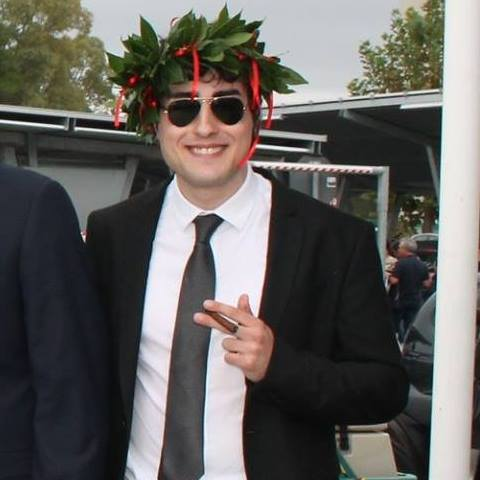
\includegraphics[width=3cm]{figures/marco.jpg}
\vspace{0.3cm}

\raisebox{-0.35ex}{
\includegraphics[width=4ex]{figures/link.png}}%
\hspace{0.05cm} /marcochiarelli

\end{figure}



%BIBLIOGRAFIA - redatta con il relativo ambiente
\begin{thebibliography}{100}
\bibitem{rif1} J. Kurose, K.W. Ross, \emph{Computer Networking. A Top-Down Approach,  sixth edition}
\bibitem{rif2} B.A. Forouzan \emph{Data Communication and Networking, fifth edition}
\bibitem{rif3} P. Oppenheimer \emph{Top Down Networking Design, third edition}
\end{thebibliography}
\end{document}



%************************************************
% Chapter 2: TEORIA DELLE CODE
%************************************************
% !TEX encoding = UTF-8
% !TEX TS-program = pdflatex
% !TEX root = ../nt.tex
% !TEX spellcheck = it-IT

%************************************************
\chapter{TEORIA DELLE CODE}
\label{cap:qtheory}
%************************************************\\

\section{PROCESSI STOCASTICI}

Modello matematico di tipo probabilistico utilizzato per andare a descrivere dei fenomeni casuali che possono essere rappresentati come funzioni di un parametro che solitamente è il tempo. $\{X(t),\ t \in T\}$. Famiglia di variabili casuali $X(t)$, indicizzate dal parametro temporale $t \in T$. Potrebbe anche essere qualche altra grandezza. Le v.a. sono definite su un unico spazio campione e che assumono valori in un certo insieme $S$. I valori assunti sono detti stati. $S$ = spazio degli stati del processo. Un processo stocastico è un insieme di funzioni del tempo. $X(t)$ generica variabile casuale. $X(t)\ \in S$. Insieme di funzioni del tempo che vengono chiamate \textbf{Realizzazioni}. Spazio campione: possibili risultati.

$X(t): T \mapsto S$ SAMPLE PATHS: realizzazioni. La cosa importante è che $X(t)$ è completamente specificato in termini probabilistici se posso scrivere la CDF congiunta (e la PDF). $X(t)$ famiglia di variabili casuali. Differenti realizzazioni. Un processo stocastico è completamente specificato con la CDF congiunta per un qualsiasi insieme (sottoinsieme) di v.a. estratte dal processo. Immaginiamo di estrarre $n$ variabili casuali:

$X(t_i),\ i=1,2,\dots,n$: estrazione di $n$ variabili casuali. Per queste devo essere in grado di scrivere la CDF congiunta:

\[
	F_{\mathbf{\underline{X}}}(\underline{x}; t) := \Pr\{X(t_1) \leq x_1,\ X(t_2) \leq x_2,\ \dots,\ X(t_n) \leq x_n\}
\]

Tale è la CDF CONGIUNTA. Ricordiamo che data una variabile casuale $\xi$, abbiamo che: $F_{\xi}(t) := \Pr\{\xi\leq t\}$. 
Qui bisogna riuscire la scrivere la CDF congiunta per queste $n$ variabili casuali estratte dal processo. In alternativa, potrei considerare la PDF congiunta, la quale è la derivata della CDF. Scriviamo la \textit{ROW VECTOR NOTATION}, generalizzando le casistiche dimensionali:

\[
	\left\{
	\begin{aligned}
	&\mathbf{\underline{X}} = (X(t_1),\ X(t_2),\ \dots,\ X(t_n)) \in\R^{n\times 1}  \\
	&\underline{x} = (x_1,\ x_2,\ \dots,\ x_n) \in\R^{n\times 1}\\
	&\underline{t} = (t_1,\ t_2,\ \dots,\ t_n) \in\R^{n\times 1}
	\end{aligned}
	\right.
\]

Ricordiamo, ancora: $[f_{\mathbf{\underline{X}}}(\underline{x}; t) = \frac{\partial{F_{\mathbf{\underline{X}}}(\underline{x}; t)}}{\partial{\underline{x}}}]$.

\subsection{CATENE DI MARKOV}

Pensiamo allo spazio degli stati $S$. Questo spazio può essere continuo o discreto. Una CATENA è un processo stocastico a stato discreto. Noi tratteremo le \textit{\textbf{CATENE DI MARKOV}}. $t$ può essere continuo o discreto. Tempo continuo o tempo discreto, rispettivamente. Quando il tempo è discreto, si parla di \textit{SEQUENZA STOCASTICA}. Eventualmente potremmo avere: $X_n,\ n=0,1,2,\dots$ ovvero diverse componenti del sistema.

Noi studieremo le CATENE DI MARKOV a tempo continuo, dette \underline{CMTC}. Categoria di processi stocastici. Per questi processi di MARKOV la relazione che intercorre tra le v.a. è molto semplice. Caratterizzazione molto semplice. Questi processi soddisfano la cosiddetta:

\begin{defn}{\textbf{PROPRIET\`A DI MARKOV}}

\[
	\Pr\{X(t) \leq x\ |\ X(t_n) = x_n,\ X(t_{n-1}) = x_{n-1},\ \dots,\ X(t_0) = x_0\} = \Pr\{X(t) \leq x\ |\ X(t_n) = x_n\}
\]

con $t > t_n > t_{n-1} >\ \dots\ > t_0$. 
\end{defn}

Questo è un processo stocastico $\{X(t),\ t\in T\}$ che soddisfa alla proprietà di MARKOV. Si tratta di una CDF condizionata. Cosa mi dice? L'evoluzione futura del processo a partire dall'istante $t_n$ non dipende dalla storia passata ma solo dallo stato finale del processo! L'evoluzione del processo da $t_n$ in poi dipende soltanto da $t_n$. Lo stato in $t_n$ riassume tutta la storia passata del processo. $\{X(t),\ t\in T\}$. Noi studieremo le catene di Markov a tempo continuo (stato discreto, tempo continuo). 

\begin{defn}{\textbf{CM omogenea}}

Invariante rispetto a traslazioni temporali degli assi:

\[
	\Pr\{X(t) \leq x\ |\ x(t_n) = x_n\} = \Pr\{X(t-t_n) \leq x\ |\ X(0) = x_n\}
\]

con $t > t_n$.
\end{defn}

Sono sostanzialmente delle catene per modellare sistemi il quale comportamento NON dipende dal tempo di osservazione. Scelta possibile dell'arco temporale. \underline{OMOGENEIT\`A}.

\begin{defn}{\textbf{COIMPLICAZIONE DELLA PROPRIET\`A DI MARKOV (\textit{tempo di soggiorno})}}

$W_i,\ i\in S$. Uno stato i qualsiasi della mia catena dev'essere una v.a. priva di memoria. Quando una v.a. casuale soddisfa alla proprietà di assenza di memoria, vale il seguente:

\[
	[\Pr\{W_i > t+\tau\ |\ W_i > t\} = \Pr\{W_i > \tau\}]
\]

Tale è la \textit{MEMORYLESS PROPERTY}.
\end{defn}

Se l'evoluzione futura del processo a partire da $t_n$ non dipende dallo stato passato del processo, non dipenderà neanche dal tempo in cui ci è stato. L'unica distribuzione di v.a. continua che soddisfa alla proprietà di assenza di memoria è la

\begin{defn}{\textbf{ESPONENZIALE NEGATIVA UNILATERA}}

\[
	\left\{
	\begin{aligned}
	&[\underline{f_{W_i}(\tau) = a\e^{-a\tau},\ \tau \geq 0}]\\
	&\left\{
	\begin{aligned}
	&F_{W_i}(\tau) = \Pr\{W_i\leq\tau\} = 1-\e^{-a\tau},\ \tau\geq 0\\
	&F_{W_i}^c(\tau) = \Pr\{W_i\geq\tau\} = \e^{-a\tau},\ \tau\geq 0
	\end{aligned}
	\right.
	\end{aligned}
	\right.
\]

\end{defn}

Unica distribuzione di probabilità che soddisfa l'assenza di memoria. Vedremo in seguito come $a := -q_{ii}$ (velocità totale di uscita dallo stato i). Velocità o equivalentemente tasso di transizione.

Proprietà di assenza di memoria per una v.a. casuale (in particolare comporta conseguenze sul tempo di soggiorno in uno stato $i$ di una CMTC):

\[
	\Pr\{W_i > t+\tau\ |\ W_i > t\} = \Pr\{W_i > \tau\}
\]	
	
Parliamone in generale.

\begin{thrm}
L'unica PDF di una v.a. continua che soddisfa alla proprietà di ASSENZA di MEMORIA è l'ESPONENZIALE NEGATIVA UNILATERA (UEN). 
\end{thrm}

\begin{proof}{\textbf{UEN MEMORYLESS PROPERTY}}
\[
	\Pr\{W_i > t+\tau\ |\ W_i > t\} = \frac{\Pr\{W_i > t+\tau,\ W_i > t\}}{\Pr\{W_i > t\}} =(\dots)
\]

Dobbiamo dimostrare questa proprietà per la UEN: $W_i>t+\tau\supseteq W_i>t \implies$

\[ 	
	(\dots) = \frac{\Pr\{W_i > t+\tau\}}{\Pr\{W_i > t\}} = \frac{\e^{-a(t+\tau)}}{\e^{-at}} = \frac{\e^{-at}\e^{-a\tau}}{\e^{-at}} = \e^{-a\tau} = \underline{\Pr\{W_i > \tau\}}
\]

La parte sottolineata sarebbe quindi la CDF complementare $F_{W_i}^c(\tau)$ della UEN.
\end{proof}

A cosa è uguale il parametro $a$? \`E uguale ad $a = -q_{ii}$, che sarebbe la velocità (totale) di uscita dallo stato $i$, ovvero la velocità totale alla quale il processo cerca di uscire dallo stato $i$. Si scrive, posto $a := -q_{ii}$:

\[
	W_i \sim EXP(-q_{ii}),\ \forall i\in S
\]

Quindi il sistema precedente diventa:

\[
	\left\{
	\begin{aligned}
	&[f_{W_i}(\tau) = -q_{ii}\e^{q_{ii}\tau},\ \tau \geq 0]\\
	&\left\{
	\begin{aligned}
	&F_{W_i}(\tau) = \Pr\{W_i\leq\tau\} = 1-\e^{q_{ii}\tau},\ \tau\geq 0\\
	&F_{W_i}^c(\tau) = \Pr\{W_I\geq\tau\} = \e^{q_{ii}\tau},\ \tau\geq 0
	\end{aligned}
	\right.
	\end{aligned}
	\right.
\]

La proprietà di assenza di memoria per $W_i$ dice che, supponendo che il processo stia soggiornando sullo stato i da $t$ unità di tempo, la probabilità che il processo mi soggiorni ancora per altre $\tau$ unità di tempo è pari alla probabilità che il processo soggiorni per $\tau$ unità di tempo. Posto $\tau$ = RESIDUO, definiamo $\Phi_{i,t}$ come tempo di soggiorno residuo nello stato i da $t$ unità di tempo, ovvero il processo si trova già da $t$ unità di tempo nello stato i! Quindi riscriviamo la MLP.

\begin{corl}

\[
	\Pr\{\Phi_{i,t} > \tau\} = \Pr\{W_i > \tau\}
\]

La distribuzione del tempo di soggiorno residuo in un tempo $t$ (LHS) è pari alla distribuzione del tempo di soggiorno (RHS). 

\[
	\left\{
	\begin{aligned}
	&[(W_i \sim \Phi_{i,t}) \sim EXP(-q_{ii})]\\
	&f_{\Phi_{i,t}}(\tau) = -q_{ii}\e^{q_{ii}\tau},\ \tau\geq 0
	\end{aligned}
	\right.
\]

\end{corl}

Nel tempo discreto la distribuzione che soddisfa la MLP è solo quella geometrica. Noi invece lavoriamo a tempo continuo. MARKOVIANIT\`A: assenza di memoria nel processo markoviano. Tempo di soggiorno residuo e tempo di soggiorno non solo hanno la stessa medesima distribuzione esponenziale (UEN), ma sono distribuite anche con lo stesso parametro $-q_{ii} = a$!

Riscriviamo la proprietà di Markov a tempo continuo! (specializzazione): Stiamo lavorando con \underline{CMTC} o CTMC (Continuos Time Markov Chain):

\[
	\Pr\{X(t_{n+1}) = x_{t_{n+1}}\ |\ X(t_n) = x_n,\ X(t_{n-1}) = x_{n-1},\ X(t_0) = x_0\} =
\]
\[
	= \Pr\{X(t_{n+1}) = x_{t_{n+1}}\ |\ X(t_n) = x_n\}
\]

$\forall x_k \in S,\ t_{n+1} > t_n > t_{n-1} >\ \dots\ > t_0$.

Chiamiamo il secondo membro \underline{probabilità di transizione}: $[\Pr\{X(t_{n+1}) = x_{n+1}\ |\ X(t_n) = x_n\}]$. Supponendo che nel tempo $t_n$ il processo si trovi in $x_n$, essa è la probabilità che al tempo $t_{n+1}$ si trovi allo stato $x_{n+1}$. Ma essa non fornisce informazioni circa quello che potrebbe accadere nel frattempo tra $t_n$ e $t_{n+1}$!

\begin{defn}{\textbf{Probabilità di Transizione da i a j}}
\[
	[\underline{p_{ij}(t,\theta) := \Pr\{X(\theta) = j\ |\ X(t) = i\}}]
\]
\end{defn}

$\forall i,j\in S$, e supponendo naturalmente che $\theta > t$.

Se la CMTC è OMOGENEA, queste probabilità di transizione non dipendono dagli istanti di tempo, ma dalla differenza dei due istanti di tempo $[\tau := \theta-t]$.

\[
	[p_{ij}(t,\theta) := \underline{P_{ij}(\tau)} = \Pr\{X(t+\tau) = j\ |\ \underline{\underline{X(t) = i}}\}]
\]

Supponendo che all'istante di tempo $t$ lo stato sia i, quella è la probabilità che dopo $\tau$ istanti di tempo lo stato sia j. Non ci riferiamo più necessariamente ai singoli istanti di tempo. Vale: $[\sum_{j\in S}{p_{ij}(\tau)} = 1]$. Distribuzione al tempo $t$: intendiamo l'insieme di queste probabilità:

\begin{defn}{\textbf{Distribuzione al tempo t}}

\[
	\pi_i(t) := \Pr\{X(t) = i\}\ \forall i\in S
\]
\end{defn}

Andiamo a considerare tutti gli stati del mio processo. Per il teorema delle probabilità totali questa probabilità la posso scrivere in tal modo:

\[
	\pi_i(t) := \Pr\{X(t) = i\} = \sum_{j\in S}{\Pr\{X(t) = i\ |\ X(0) = j\}\Pr\{X(0) = j\}} = \sum_{j\in S}{\underline{p_{ji}(t)}\underline{\pi_j(0)}}
\]

Quindi questa distribuzione al tempo $t$ la possiamo ottenere come somma di prodotti tra la distribuzione iniziale e la probabilità di transizione da j ad i. Possiamo inoltre, dato $\pi_j(0)$, conoscere qualsiasi CDF congiunta. Per ogni processo particolare posso scriverle facilmente... A tempo continuo le probabilità di transizione dipendono però dal tempo! $(\dots) = \mathord{\cdot}(t)$! Per semplificare la vita, sono state introdotte delle quantità legate a $\underline{p_{ji}(t)}$, generalmente anch'esse dipendenti dal tempo, ma che, nel caso in cui la CMTC sia OMOGENEA, sono invece costanti. Queste quantità sono quindi costanti e sono chiamate TASSI o \textit{VELOCIT\`A DI TRANSIZIONE}. Ciò che NON è costante è invece la probabilità di transizione.

\subsubsection{Tassi di Transizione}

\begin{defn}{\textbf{TASSI (o VELOCIT\`A) di transizione}}

Relazione che lega i tassi di transizione alle probabilità di transizione.
Se la catena è regolare:

\[
	\left\{
	\begin{aligned}
	&\exists q_{ij} := \lim_{\Delta t\to 0}{\frac{p_{ij}(\Delta t)}{\Delta t}},	\forall (i\neq j)\in S\\
	&\exists q_{ii} := \lim_{\Delta t\to 0}{\frac{p_{ii}(\Delta t)-1}{\Delta t}} \leq 0
	\end{aligned}
	\right.
\]

$\forall i,j\ \in S$.
\end{defn}

Si può dimostrare che questi limiti, queste quantità, esistono se la CMTC è REGOLARE, ovvero se:

\begin{defn}{\textbf{CMTC REGOLARE}}

\[
	\forall X(0),\ [\underline{\cardinality{transizioni(\Delta t < +\infty)} < +\infty}]
\]
\end{defn}

Questo deve valere per qualunque stato iniziale. $-q_{ii} \geq 0$. Supponiamo che lo stato del processo in $t$ sia $i$ $\iff X(t) = i$. La probabilità che in un intervallo $\Delta t$ tendente a 0 ($\iff \Delta t \to 0$) vi sia una transizione al di fuori di i è: $[-q_{ii}\Delta  t + o(\Delta t)]$.
Ragioniamo invece su $p_{ii}(\Delta t)$: essa rappresenta la probabilità che lo stato presente sia $i$ e tra $\Delta t$ unità di tempo lo stato sia di nuovo $i$. Tale probabilità non mi dice nulla su tutte le possibili transizioni che ci possono essere tra $t$ e $t+\Delta t$.

$1-p_{ii}(\Delta t),\ \Delta t \to 0$ è la probabilità che dopo $\Delta t$ unità di tempo lo stato NON sia più $i$, partendo da $i$ (prob. che vi sia una transizione). Quando $\Delta t \to 0$, questa probabilità tende alla probabilità di leaving dallo stato $i$. Quindi invertendo la seconda equazione del precedente sistema troviamo che al limite essa è uguale a: $[-q_{ii}\Delta t + o(\Delta t)]$. La probabilità è tanto più grande quando $q_{ii}$ è alto in modulo! Più velocemente esce, più è probabile che esca! Più grande è il valore $\abs{q_{ii}}$, più il processo cerca di uscire velocemente, e quindi con maggior probabilità vi riuscirà $\implies \abs{q_{ii}} \uparrow \implies$ processo più velocemente tende ad uscire.

$-q_{ii}$ è quindi la velocità alla quale un processo lascia lo stato $i$. In sostanza, $-q_{ii}$ rappresenta il numero medio di transizioni al di fuori di $i$ $\forall$ unità di tempo \newline
\underline{in cui il processo si trova nello stato $i$}.

Prendiamo per esempio due diverse realizzazioni dello stesso processo: $\{X^{(1)}(t),\ X^{(2)}(t)\}$. Per $X^{(1)}(t)$ abbiamo diversi soggiorni nello stato i. Supponiamo che la somma delle durate di soggiorno in $i$ facciano $1s$. Durante questa unità di tempo in cui il processo si trova in $i$, si trovano 7 transizioni al di fuori di $i$. Per $X^{(2)}(t)$, supponiamo lo stesso caso ma con 5 transizioni. Abbiamo detto che: $-q_{ii}$ è il numero medio di transizioni al di fuori dello stato $i$. Una transizione uscente segue un \underline{tempo di soggiorno}. $-q_{ii}$ rappresenta quindi anche il tempo medio di soggiorno. Ricordando che $f_{W_i}(\tau) = -q_{ii}\e^{q_{ii}\tau}$, abbiamo che:

\[
	\E[W_i] = \frac{1}{-q_{ii}}
\]

Se calcoliamo il valor medio (la media) di $f_{W_i}(\tau)$, esce proprio $(\frac{1}{-q_{ii}})$; tanto più grande è $q_{ii}$, tanto basso sarà il tempo di soggiorno in media.

Significato di $q_{ij}$. Supponiamo che attualmente il processo si trovi in $i$. La probabilità che in un intervallo di tempo infinitesimo ($\Delta t \to 0$) vi sia una transizione $ij$, ($i \rightarrow j$), è uguale alla probabilità $q_{ij}\Delta t + o(\Delta t)$. Consideriamo $p_{ij}(t)$. Non mi dice nulla, essendo una probabilità di transizione, su cosa sia eventualmente accaduto nel rispettivo intervallo di tempo tra la transizione.

Accade quindi che:

\[
	[\lim_{\Delta t \to 0}{\frac{p_{ij}(t)}{\Delta t}} = q_{ij}]
\]

(probabilità tanto più grande quanto più grande è $q_{ij}$).
La velocità è $q_{ij}$. Rappresenta una velocità alla quale si verifica la transizione $i \rightarrow j$. Ecco perché viene detto TASSO (o VELOCIT\`A) di TRANSIZIONE da $i$ a $j$. Ma è anche in sostanza il numero medio di transizioni da $i$ a $j$ $(i \rightarrow j) \ \forall$ unità di tempo in cui il processo si trova nello stato i$i$ Ragioniamo di nuovo sulle due funzioni rappresentanti due diverse realizzazioni dello stesso processo. Supponiamo sempre che la durata complessiva di un soggiorno in $i$ sommi temporalmente ad 1. $q_{ij}$ si differenzia da $-q_{ii}$ in quanto rappresenta il numero medio di transizioni ($i \rightarrow j$).

\[
	\sum_{(j\neq i)\in S}{q_{ij}} = \sum_{(j\neq i)\in S}{(\lim_{\Delta t \to 0}{\frac{p_{ij}(\Delta t)}{\Delta t}})} = \lim_{\Delta t \to 0}{\sum_{(j\neq i)\in S}{(\frac{p_{ij}(\Delta t)}{\Delta t})}} = (\dots)
\]

Considerando uno stato $i$ qualsiasi, questa sommatoria fa 1: $\iff \sum_{j\in S}{p_{ij}(\Delta t)} = 1$. Quindi:

\[
	(\dots) = \lim_{\Delta t \to 0}{\frac{1-p_{ii}(\Delta t)}{\Delta t}} = \underline{\underline{-q_{ii}}}
\]

La quale è la velocità \underline{totale} di uscita dallo stato $i$. Introduciamo ora una seconda quantità: $[\tau_{i,j} = \frac{q_{ij}}{-q_{ii}}]$, ovvero la probabilità che il processo, lasciando lo stato i, faccia una transizione verso lo stato $j$. 

Supponiamo che $q_{ij}=10,\ q_{ik}=30,\ q_{ih}=60$... mediamente vi siano quindi 100 transizioni uscenti. $-q_{ii} = \sum_{(j\neq i)\in S}{q_{ij}} = 100$. Abbiamo che:

\[
	\left\{
	\begin{aligned}
	&\tau_{i,j} = \frac{10}{100} = 0.1\\
	&\tau_{i,h} = \frac{60}{100} = 0.6\\
	&\tau_{i,k} = \frac{30}{100} = 0.3
	\end{aligned}
	\right.
\] 

$\tau_{i,j}$ è quindi alla fine la probabilità che, supponendo di lasciare $i$, la transizione sia verso $j$. LASCIANDO LO STATO $i$, $\exists$ UNA TRANSIZIONE VERSO LO STATO $j$.

Distribuzione al tempo $t$. Ci sono dei sistemi di equazioni differenziali che legano la distribuzione al tempo $t$ ai tassi di transizione:

\[	
	\left\{
	\begin{aligned}
	&\underline{\pi_i}(t) := \Pr\{X(t) = i\},\ \forall i\in S\\
	&\frac{d \pi_i(t)}{dt} = \sum_{j\in S}{q_{ji}\pi_j(t)},\ \forall i\in S
	\end{aligned}
	\right.
\]

Di queste equazioni differenziali ve n'è una $\forall s\in S$ della nostra catena. Nella maggior parte dei casi, non ci serve $\pi_i(t)$, ma una distribuzione a regime (costante). A regime serve la rispettiva distribuzione a regime (dopo un tempo molto grande). Ci sono delle condizioni in base alla quale $\pi_i(t) \to K \neq \mathord{\cdot}(t)$ (distribuzione di equilibrio, a regime). Ma quali sono queste condizioni?

\subsection{Probabilità a regime}

Quali sono le condizioni di esistenza delle probabilità di stato a regime? Introduciamo alcune definizioni. Consideriamo uno stato $i \in S$ della mia \underline{CMTC}. Diciamo che lo stato $(i\in S)$ è \textit{TRANSITORIO} se c'è una probabilità non nulla che il processo non torni più in quello stato dopo che esso viene lasciato. Si dirà \textit{RICORRENTE} in caso contrario (se con probabilità 1 torni nello stato $i$ dopo averlo lasciato). Ai fini della distribuzione di regime, a noi interessano i RICORRENTI (gli stati ricorrenti). Sia $M_i$ il tempo medio di ritorno (o \underline{di ricorrenza} nello stato $i$). Per tempo di ritorno si intende il tempo che passa da \underline{due ingressi consecutivi} nello stato $i$. $M_i$ dice quanto dura in media questo tempo (ovviamente guardando tutte le possibili realizzazioni, altrimenti sarebbe costante). Si consideri una finestra temporale ($M_i$), è contemplato in media un solo soggiorno in $i$! (UN SOLO tempo di soggiorno). Se questo valore diverge ($\iff M_i \to +\infty$), lo stato è detto \textit{RICORRENTE NULLO}. Se $M_i$ converge parliamo di STATO \textit{RICORRENTE NON NULLO}.

Consideriamo ora un sottoinsieme proprio dello spazio degli stati $A\subset S\ |\ \bar{A} \cup A = S$. $A$ comprende una parte degli stati, e non può coincidere con $S \iff \bar{A} = S \setminus (A\neq \emptyset)$.

Vale:

\begin{thrm}
$A$ chiuso se:

\[
	\sum_{i\in A}{\sum_{j\in\bar{A}}{q_{ij}}} = 0
\]
\end{thrm}

Significa che una volta che il processo entra in $A$, NON esce da $A$! In particolare, chiamiamo \textit{STATO TRAPPOLA} od \textit{ASSORBENTE} uno stato $i$ per il quale: $ [q_{ii} = -q_{ii} = 0]$ (Il processo NON esce più da quello stato). Uno STATO TRAPPOLA corrisponde ad un insieme chiuso costituito da solo quello stato.

\begin{defn}{\textbf{CM IRRIDUCIBILE}}

Una CTMC è \underline{\underline{IRRIDUCIBILE}} se $\nexists$ insiemi chiusi $\iff$ Tutti gli stati COMUNICANO tra di loro. Da $i$ a $j$ ci arrivo (magari passando da altri stati), ma ci arrivo sempre prima o poi! $i \leftarrow\rightarrow j\ \forall i,j\in S$.

\end{defn}

Abbiamo quindi tre caratterizzazioni di stato: (tre diversi possibili tipi di stato):

\begin{itemize}

\item{\textit{TRANSITORI}};
\item{\textit{RICORRENTI NULLI}};
\item{\textit{RICORRENTI NON NULLI}}.

\end{itemize}

\begin{corl}{\textbf{Omogeneità dei tipi di stato per CM IRRIDUCIBILE}}

Qualora una CM sia IRRIDUCIBILE $\implies$ allora tutti gli stati sono dello stesso tipo.

\end{corl}

Concetto molto forte. CATENA IRRIDUCIBILE $\iff$ tutti gli stati comunicano $\iff$ tutti gli stati sono dello stesso tipo. Ricordiamo:

\[
	[\frac{d \pi_i(t)}{dt} = \sum_{j\in S}{q_{ji}\pi_j(t)}]
\]

\begin{defn}{\textbf{PROBABILIT\`A LIMITE}}
\[
	[\pi_i := \lim_{t\to\infty}{\pi_i(t)}]
\]
$\forall i\in S$.
\end{defn}

Se una CATENA è OMOGENEA, IRRIDUCIBILE (Quando una CATENA è OMOGENEA i tassi di transizione sono COSTANTI), allora:

\[
	\exists \lim_{t\to\infty}{\pi_i(t)} := \pi_i \neq \mathord{\cdot} \pi_i(0)
\]

Se vogliamo avere delle distribuzioni a regime, vogliamo che questa quantità esista finita (limite esistente e convergente). In particolare non devono dipendere dalle probabilità di \underline{stato iniziali}. In tal caso il sistema di equazioni differenziali collassa in un sistema di equazioni algebriche lineari:

\[
	[\sum_{j\in S}{q_{ji}\pi_j} = 0]
\]

$\forall i\in S$. Le derivate vanno quindi a 0 $\iff \pi_i(t) \tendsto{t\to\infty} \pi_i$. Questo sistema è OMOGENEO (sicuramente comprende la soluzione nulla). Tante soluzioni quanti sono gli stati del processo. SE la soluzione nulla fosse l'unica soluzione, gli stati saranno tutti TRANSITORI o tutti RICORRENTI nulli e non avremmo quindi una distribuzione di regime ($\iff \nexists \pi_i$). Se così non fosse invece, in tal caso le soluzioni saranno un numero infinito, che differirranno per una \underline{costante moltiplicativa} tra di loro. Se sono infinite (tutte linearmente dipendenti), tra tutte queste le filtriamo con la cosiddetta condizione di normalizzazione. In tal caso gli stati saranno tutti \underline{RICORRENTI NON NULLI}.

\begin{defn}{\textbf{ERGODICIT\`A}}

\[
	\left\{
	\begin{aligned}
	&\sum_{j\in S}{q_{ji}\pi_j} = 0,\ \forall i\in S\\
	&\sum_{i\in S}{\pi_i} = 1
	\end{aligned}
	\right.
\]

$\exists SOL$? Se esiste, in tal caso la CATENA è detta \textit{ERGODICA} (proprietà di ERGODICIT\`A). \underline{CMTC} \{OMOGENEA, IRRIDUCIBILE, (STATI RICORRENTI NON NULLI)\}.\end{defn}

Innanzitutto, si verifichi l'OMOGENEIT\`A guardando i tassi di transizione (diagrammi di stato). Devono essere costanti (OMOGENEA, \underline{\underline{IRRIDUCIBILE}} (stati dello stesso tipo)). Basterebbe, per verificare che gli stati siano TUTTI ricorrenti non nulli, verificare questa proprietà per UN SOLO STATO! Ma a questo punto, senza ragionare su $M_i$, ragiono sull'equazione e la risolvo, sperando di risolverla e di trovare UNA ed UNA SOLA soluzione.

\begin{corl}{\textbf{Caratterizzazione dell'Ergodicita'}}

Se abbiamo una [CMTC OMOGENEA, IRRIDUCIBILE e con un numero di stati finito $(\iff\cardinality{stati}<+\infty)$], sicuramente essa è \underline{ERGODICA}].

\end{corl}

Abbiamo detto che $\pi_i,\ i\in S$ sono le probabilità limite, QUANTIT\`A valutate IN VERTICALE, ed hanno a che fare con le distribuzioni di regime. MA è anche la frazione di tempo a regime in cui lo stato sia $i$.

\subsection{ERGODICIT\`A}

Condizioni di ERGODICIT\`A per una CMTC: \{OMOGENEA, IRRIDUCIBILE, con STATI RICORRENTI NON NULLI\} $\implies [\exists \lim_{t\to\infty}{\pi_i(t)} := \pi_i]$. Una volta veriifcate queste due proprietà, non c'è bisogno di verificare che gli stati siano tutti RICORRENTI NON NULLI. In maniera più semplice si tenta di risolvere quel sistema sperando che abbia una soluzione non banale. Diagramma dei tassi di transizione: \{Cerchi = Stati, Archi = Transizioni, pesate con i tassi di transizione\}. Se questi tassi non sono dipendenti dal tempo allora la catena è OMOGENEA. 

\[
	[\underline{\pi_i} = \lim_{t\to\infty}{(\pi_i(t) = \Pr\{X(t)=i\})},\ \forall i\in S
\]

La distribuzione di regime ha ovviamente a che fare con le probabilità limite. Immaginiamo che la catena sia ERGODICA. $\pi_i$ = probabilità che a regime lo stato sia $i$. Se la catena è \underline{ergodica}, allora a $\pi_i$ possiamo attribuire un altro significato: frazione del tempo (A REGIME) in cui lo stato sia $i$:

\[
	[\pi_i = \lim_{t\to\infty}{\frac{T_i(t)}{t}}]
\]

dove $T_i(t)$ è il tempo trascorso dal processo \underline{nello stato $i$} sino al tempo $t$. (SINGOLA REALIZZAZIONE). \`E come se stessimo guardando una singola realizzazione del processo. Presa una finestra $[0,t) \leftarrow T_i(t)$. Fino al tempo $t$. Se calcolo $\frac{T_i(t)}{t}$, allora ottengo la frazione di tempo nel quale il processo è stato nello stato $i$ nell'intervallo di tempo definito dalla finestra temporale scelta.

es. $\pi_i = 0.2 \implies$ per il 20\% il processo a regime si è trovato in $i$. $\pi_i\tau$ rappresenta il tempo in media nel quale il processo si è trovato nello stato $i$ durante la finestra temporale di durata $\tau$. $\pi_i$ è da valutare sull'INSIEME delle realizzazioni.

Consideriamo $N(t)$ processo stocastico che rappresenta il numero di clienti (\#) in un sistema a coda. Esaminiamo un certo numero di realizzazioni.

Dal momento che $\pi_i(t)$ è una probabilità, essa va valutata in verticale. Supponiamo che:

\[
	\left\{
	\begin{aligned}
	&n_R := \cardinality{realizzazioni\ di\ N(t)}\\
	&n_i(t) := n_i = \cardinality{realizzazioni\ con\ stato\ i\ nell'istante\ t}
	\end{aligned}
	\right.
\]

$(\frac{n_i}{n_R})$ rappresenta la frazione delle $n_R$ realizzazioni con stato pari ad $i$ in $t$. Quando $n_R$ cresce, $\iff n_R \uparrow ,\ (\frac{n_i}{n_R}) \tendsto{}$ probabilità che lo stato del processo sia $i$.

Rispettivamente:

\begin{thrm}{\textbf{Probabilità Limite}}

\[
	\lim_{n_R\to\infty}{(\frac{n_i}{n_R})} = \pi_i(t) = \Pr\{X(t)=i\}
\]
\end{thrm}

Tutto questo a regime! Abbiamo considerato $\pi_i$ valutandola con un numero molto grande di realizzazioni. Guardando invece ad una singola realizzazione di tempo molto grande ($\iff t\to +\infty$), abbiamo che: $\underline{\pi_i} = \lim_{t\to\infty}{\frac{T_i(t)}{t}}$, che sarebbe la frazione in cui il processo si è trovato in $i$ nella finestra temporale $[0,t)$.

\begin{thrm}{\textbf{Mapping VERTICALE ORIZZONTALE}}

Se c'è l'ERGODICIT\`A abbiamo che:

\[
	\underline{\pi_i} = \lim_{n_R\to\infty}{(\frac{n_i}{n_R})} = \pi_i(t) = \Pr\{X(t)=i\} = \lim_{t\to\infty}{\frac{T_i(t)}{t}}
\]
\end{thrm}

Si consideri ora: $\bar{N} = \sum_{i=0}^\infty{i\pi_i}$. Questo è la media del numero di clienti. Numero medio di clienti del sistema a regime (si noti l'estremo superiore della sommatoria). Ma se il processo è ERGODICO, la media di insieme coincide con la media temporale. Nella pratica si suppone l'\underline{ergodicità}, si procede in orizzontale. Si consideri $\lim_{t\to\infty}{\bar{N_t}}$. Senza il limite essa rappresenta il valore medio assunto da quelle funzioni: $\bar{N_t} := \frac{1}{t}\int_0^t{N(\tau)d\tau}$ (MEDIA TEMPORALE) durante la finestra temporale $[0,t)$. Se c'è l'ERGODICIT\`A allora questa quantità, AL LIMITE di $t\to\infty$ coincide con $\bar{N} \iff [\lim_{t\to\infty}{\bar{N_t}} = \bar{N}]$ = VALORE DI REGIME.

\subsubsection{ERGODICIT\`A (RECAP)}

$\{\pi_i,\ \pi_i\tau\}$ rappresentano rispettivamente la probabilità che \underline{a regime} il processo si trovi in $i$, ed il tempo medio che il processo si trova in $i$ nella finestra temporale di lunghezza $\tau$. $M_i$ = tempo medio di ritorno nello stato $i$. Supponiamo di avere $\tau = M_i$. Sarebbe il tempo tra due ingressi consecutivi nello stato $i$ = tempo di ricorrenza. VALOR MEDIO $M_i$. \`E necessariamente un tempo di soggiorno. Quindi: 

$\pi_iM_i$ = tempo medio trascorso nello stato $i$ durante la finestra temporale $\tau = M_i$. Ma abbiamo \underline{un solo soggiorno} durante $M_i \iff [\underline{\pi_iM_i} = \E[W_i] = \frac{1}{-q_{ii}}]$. Invertendo troviamo: $M_i = \frac{1}{-q_{ii}\pi_i}$ (tempo medio di ricorrenza). Ricordiamo che:

\[
	\underline{f}_{W_i}(\tau) = -q_{ii}\e^{q_{ii}\tau},\ \tau\geq 0
\]

Ed avendo un solo soggiorno $\underline{\pi_iM_i}$ rappresenta il TEMPO \underline{MEDIO DI SOGGIORNO}. Possiamo dare una formulazione matriciale dell'insieme di equazioni differenziali:

\[
	\left\{
	\begin{aligned}
	&\frac{d \pi_i(t)}{dt} = \sum_{j\in S}{q_{ji}\pi_j(t)},\ \forall i\in S\\
	&\frac{d \underline{\pi(t)}}{dt} = \underline{\pi(t)}\underline{Q}
	\end{aligned}
	\right.
\]

$\underline{\pi}$ è il vettore riga delle probabilità di stato al tempo t, indicizzato da $i$. Nel caso di ERGODICIT\`A ovviamente vale che: $[\underline{\pi}\underline{Q} = \underline{0}]$ (vettore nullo).

\subsection{CMTC Nascita e Morte}

Caso particolare di CMTC, utili per lo studio dei sistemi a coda. CATENE DI NASCITA E MORTE per una CMTC. Caso particolare di CMTC. Sono dette così perché si prestano bene a modellare una evoluzione, dinamica di una popolazione (dimensione della popolazione). Abbiamo incrementi o decrementi di stato UNITARI $\iff\ \{i++,\ i--\}$. Ci interessano molto. Sono delle catene definite sullo spazio degli stati $S = \{0,1,2,\ \dots\}$. Tale spazio può essere di dimensione illimitata. Ma tipicamente lo spazio per noi sarà tale che $\cardinality{S} < +\infty$. Catene caratterizzate da fatto che vi sono incrementi/decrementi solo unitari.

Sia $N(t) = i$, quello che può accadere è che: $\{N(t) = i \to i+1\ \lor\ N(t) = i \to i-1\}$. Nel DTT (diagramma dei tassi di transizione), gli archi ricordiamo che rappresentano delle transizioni, e sono pesati dai tassi (o velocità) di transizione. DTT sarà fatta con cerchi che rappresentano gli stati, e gli archi rappresentanti le transizioni, pesati con i rispettivi tassi (o velocità).

\begin{center}
\begin{tikzpicture}[->, >=stealth', auto, semithick, node distance=1.9cm]
\tikzstyle{every state}=[fill=white,draw=black,thick,text=black,scale=1]
\node[state]    (0)                     {$0$};
\node[state]    (1)[right of=0]   {$1$};
\node[state]    (2)[right of=1]   {$2$};
\node[state] (d) [right of=2] {\ldots};
\node[state]    (im1)[right of=d]   {$i-1$};
\node[state]    (i)[right of=im1]   {$i$};
\node[state]    (ip1)[right of=i]   {$i+1$};
\node[state]    (d2)[right of=ip1]  {\ldots};
\path
(0) edge[bend left]     node{$\lambda_0$}         (1)
(1) edge[bend left]     node{$\lambda_1$}         (2)
    edge[bend left,below]    node{$\mu_1$}            (0)
(2) edge[bend left]     node{$\lambda_2$}           (d)
    edge[bend left,below]    node{$\mu_2$}             (1)
(d) edge[bend left]         node{$\lambda_{i-2}$}   (im1)
	edge[bend left,below]   node{$\mu_3$}          (2)
(im1) edge[bend left]       node{$\lambda_{i-1}$}  (i)
	  edge[bend left,below]   node{$\mu_{i-1}$}     (d)
(i)   edge[bend left]   node{$\lambda_i$}      (ip1)
      edge[bend left,below]  node{$\mu_i$}          (im1)
(ip1) edge[bend left]       node{$\lambda_{i+1}$}  (d2)
	 edge[bend left,below]   node{$\mu_{i+1}$}      (i)
(d2) edge[bend left,below]   node{$\mu_{i+2}$}     (ip1);
\end{tikzpicture}
\end{center}

Tipicamente in un DTT per una catena di questo tipo abbiamo che sopra ci sono le nascite ($\lambda_i$), e sotto vi sono le morti ($\mu_i$). Rispettivamente:

\begin{defn}{\textbf{Tassi di nascita e morte}}

\[
	\left\{
	\begin{aligned}
	&\lambda_i :=\ tasso\ di\ nascita\ sullo\ stato\ i\\
	&\mu_i :=\ tasso\ di\ morte\ nello\ stato\ i
	\end{aligned}
	\right.
\]
\end{defn}

Se questi valori sono COSTANTI $\iff$ la CATENA è OMOGENEA. Se la catena è IRRIDUCIBILE: tutti gli stati comunicano $\implies [\exists\pi_i = \lim_{t\to\infty}{\pi_i(t)}]\ \forall i\in S$. Il numero di stati però NON è finito! $(\iff \cardinality{S} = +\infty)$. Quindi dobbiamo cercare di risolvere il sistema:

\[
	\left\{
	\begin{aligned}
	&\sum_{j=0}^\infty{q_{ji}\pi_j} = 0\\
	&\sum_{i=0}^\infty{\pi_i} = 1\ (CONDIZIONE\ DI\ NORMALIZZAZIONE)
	\end{aligned}
	\right.
\]

Abbiamo che: $-q_{00} = \lambda_0$ (velocità totale di uscita dallo stato 0). Quindi: $-\lambda_0\pi_0 + \mu_1\pi_1 = 0$ per lo stato 0, poi dato che vale: $-q_{11}=\lambda_1 + \mu_1$, allora per lo stato 1: $\lambda_0\pi_0 -( \lambda_1+\mu_1)\pi_1 + \mu_2\pi_2 = 0$. Genericamente allo stato i abbiamo:

\[
	"i" \rightarrow\ \lambda_{i-1}\pi_{i-1} - (\lambda_i +\mu_i)\pi_i + \mu_{i+1}\pi_{i+1} = 0
\]

Queste si chiamano EQ. DI BILANCIAMENTO TOTALE. Noi scriviamo le equazioni in generale per una \underline{CMTC ERGODICA}. $\sum_{j\in S}{q_{ji}\pi_j} = 0\ \forall i\in S$. Proviamo a tirare fuori il termine della sommatoria per $j=i$:

\[
	\implies \sum_{(j\neq i)\in S}{q_{ji}{\pi_j}} = -q_{ii}\pi_i
\]

Generalizzando possiamo scrivere le:


\begin{thrm}{\textbf{EQUAZIONI DI BILANCIAMENTO TOTALE}}

\[
	\sum_{(j\neq i)\in S}{q_{ji}\pi_j} = \sum_{(j\neq i)\in S}{q_{ij}\pi_i}
\]

\end{thrm}

Esse esprimono il fatto che a regime (od equilibrio), la frequenza delle transizioni entranti nello stato $i$ eguaglia la frequenza delle transizioni uscenti dallo stato $i$. \`E sostanzialmente un altro modo di scrivere: $\sum_{j\in S}{q_{ji}\pi_j} = 0\ \forall i\in S$. Il numero medio (per unità di tempo) di transizioni entranti nello stato $i$ è uguale al numero medio di transizioni uscenti nello stato $i$. $q_{ji}\pi_j$ è la frequenza (quindi adimensionale) delle transizioni dallo stato $j$ allo stato $i$. Numero medio di transizioni nello stato $i$ (per unità di tempo).

$q_{ji}$ = numero medio di transizioni da $j$ ad $i\ \forall$ unità di tempo in cui il processo si trova nello stato $j$, mentre $\pi_j$ è una frazione di tempo. Ricordiamo che scelta ad esempio una finestra temporale $\tau=1s$, allora il prodotto $\pi_j\tau$ rappresenta il tempo medio trascorso durante questa finestra temporale ($\tau=1s$) dal processo nello stato $j$. Se facciamo $q_{ji}\pi_j$ otteniamo invece il numero medio di transizioni da $j$ ad $i$ $\forall$ unità di tempo. 

L'intera equazione dice che all'equilibrio la frequenza delle transizioni verso lo stato $i$ è pari alla frequenza di transizioni uscenti dallo stato $i$. All'equilibro il flusso entrante nello stato $i$ è pari al suo flusso uscente. Si eguaglia praticamente ($\forall$ stato), flusso entrante (IN) e flusso uscente (OUT). Quindi dobbiamo bilanciare il flusso caso per caso.

Consideriamo l'equazione di bilanciamento per il generico stato $i$:

\[	
	(\lambda_{i-1}\pi_{i-1} + \mu_{i+1}\pi_{i+1} = IN) = ((\lambda_i +\mu_i) = OUT)
\]

Per lo stato 0 abbiamo: $\mu_1\pi_1 = \lambda_0\pi_0$.
Vale per qualunque CMTC \underline{ERGODICA}.

\begin{thrm}{\textbf{EQUAZIONI DI BILANCIAMENTO TOTALE generalizzate}}

Possiamo considerare $(A \subset S) \supset \{statuses\}$. Si immagini di considerare come macrostati gli insiemi di stato $\{0,\ \dots,\ i\}$. Valgono le eq. di bilanciamento totale generalizzate: Flusso uscente da A = flusso entrante in A:

\[
	\sum_{j\in \bar{A},i\in A}{q_{ij}\pi_i} = \sum_{j\in \bar{A},i\in A}{q_{ji}\pi_j}
\]

\end{thrm}

Inoltre, ne deriva che per una BDCMTC abbiamo di conseguenza:

\begin{corl}{\textbf{EQUAZIONI DI BILANCIAMENTO TOTALE GEN. per BD-CMTC}}

\[
	[(\lambda_i\pi_i)_{OUT} = (\mu_{i+1}\pi_{i+1})_{IN}]
\]

\end{corl}

Tentiamo ora di eguagliare il flusso sulla frontiera verticale tra due stati. Otteniamo:

\begin{thrm}{\textbf{EQUAZIONI DI BILANCIAMENTO LOCALE}}


\[
	\pi_iq_{ij} = \pi_jq_{ji}
\]

\end{thrm}

QUESTE valgono soltanto IN CASI PARTICOLARI (BDCMTC). Le GLOBALI e quelle GLOBALI GENERALIZZATE valgono invece SEMPRE per una CMTC.

Si considerino queste equazioni trovate per una BDCMTC:

\[
	\left\{
	\begin{aligned}
	&\lambda_i\pi_i = \mu_{i+1}\pi_{i+1},\ i\geq 0\\
	&\sum_{i=0}^\infty{\pi_i} = 1\ as\ C.N.
	\end{aligned}
	\right.
\]

Quindi abbiamo: $\pi_{i+1} = \frac{\lambda_i \pi_i}{\mu_{i+1}}$. Prendiamo $(i=0) \implies \pi_1 = \pi_0 \frac{\lambda_0}{\mu_1}$. Andando avanti ricorsivamente troviamo:

\[
	\left\{ 
	\begin{aligned}
	&i=1 \implies \pi_2 = \pi_1 \frac{\lambda_1}{\mu_2} = (\pi_0 \frac{\lambda_0}{\mu_1})\frac{\lambda_1}{\mu_2}\\
&i=2 \implies \pi_3 = \pi_2 \frac{\lambda_2}{\mu_3} = (\dots) = \pi_0 \frac{\lambda_0\lambda_1\lambda_2}{\mu_1\mu_2\mu_3}\\
&i-1 \implies \underline{\pi_i} = \pi_0 \frac{\lambda_0\lambda_1\lambda_2\dots\lambda_{i-1}}{\mu_1\mu_2\dots\mu_i} = \pi_0\prod_{k=0}^{i-1}{\frac{\lambda_k}{\mu_{k+1}}},\ i \geq 1
	\end{aligned}
	\right.
\]

Abbiamo quindi trovato le espressioni per le:

\begin{defn}{\textbf{Probabilità a regime}}

\[
	[\underline{\pi_i} = \pi_j\prod_{k=j}^{i-1}{\frac{\lambda_k}{\mu_{k+1}}}] = \mathord{\cdot}(\pi_j)
\]
\end{defn}

Adesso vogliamo mettere in gioco la condizione di normalizzazione: Quindi essa diventa:

\[
	[\pi_0 + \sum_{i=1}^{\infty}{\pi_i} = 1] \implies \pi_0 + \sum_{i=1}^{\infty}{\pi_0\prod_{k=0}^{i-1}{\frac{\lambda_k}{\mu_{k+1}}}} = 1 = \pi_0(1 + \sum_{i=1}^{\infty}{\prod_{k=0}^{i-1}{(\frac{\lambda_k}{\mu_{k+1}})}}) = 1 \implies
\]
\[
	\pi_0 = \frac{1}{1 + \sum_{i=1}^{\infty}{\prod_{k=0}^{i-1}{(\frac{\lambda_k}{\mu_{k+1}})}}}
\]

with:

\[
	\pi_i = [\pi_0 \prod_{k=0}^{i-1}{\frac{\lambda_k}{\mu_{k+1}}}],\ i \geq 1
\]

\begin{corl}

Se la sommatoria a denominatore di $\pi_0$ converge, allora la soluzione esiste. Quindi:

\[
	\pi_i = [\frac{1}{1 + \sum_{i=1}^{\infty}{\prod_{k=0}^{i-1}{(\frac{\lambda_k}{\mu_{k+1}})}}}] \prod_{k=0}^{i-1}{\frac{\lambda_k}{\mu_{k+1}}},	 i \geq 1
\]
\end{corl}

\newpage

\subsection{PROCESSO DI POISSON}

\`E un caso particolare di BDCMTC nel quale i tassi di nascita sono costanti e pari a $\lambda_i = \lambda \neq \mathord{\cdot}(i)\ \land\ \mu_i = 0\ \forall i\in S$. \`E sottinteso che il processo sia omogeneo. Il processo è di pura nascita. Lo spazio degli stati è il seguente: $S = \{0,1,2,\ \dots\}$. Tutti gli stati sono TRANSITORI (una volta uscito da uno stato NON vi ritorno più) $\implies \nexists (\pi_i \neq \mathord{\cdot}(t))$. 

\[
	\left\{
	\begin{aligned}
	&\frac{d \pi_i(t)}{dt} = \sum_{j\in S}{q_{ji}\pi_j(t)},\ \forall i\in S\\
	&\underline{\underline{\pi_0(0)}} = 1
	\end{aligned}
	\right.
\]

dove l'ultima equazione del sistema rappresenta la condizione iniziale, sempre da rispettare. Per un processo di POISSON abbiamo che la distribuzione soddisfa alla seguente:

\begin{defn}{\textbf{Funzione massa di probabilità per un Processo di POSSION}}

\[
	\pi_i(t) = \Pr\{X(t) = i\} = \frac{(\lambda t)^i}{i!}\e^{-\lambda t},\ t\geq 0,\ \forall i\in S
\]

\end{defn}

Questa espressione mi ricorda la distribuzione di POISSON con parametro $(a := \lambda t)$. Avendo una v.a. distribuita con Poisson con parametro $a \implies a = \E[X]$. Disegnamo una possibile realizzazione del processo. Supposto che evolva a partire dallo stato 0. Abbiamo:

$\{\tau_1 = W_1,\ \tau_2 = W2,\ \dots,\ \tau_n = t_n-t_{n-1}\}$. Possiamo quindi scrivere la PDF del tempo di soggiorno negli stati:

\[
	[f_{\tau_n}(r) = \lambda\e^{-\lambda r},\ r \geq 0]
\]

ove (\underline{$\tau_n$ = tempo di soggiorno negli stati}). Queste variabili casuali sono distribuite secondo Poisson. Il processo di POISSON modella gli arrivi dei pacchetti alle code dei router. Arrivi dei clienti in un sistema a coda. Supponiamo di utilizzare al posto di $X(t)$, $A(t)$. \textit{ARRIVAL}. Posso dire che questo processo CONTEGGIA gli arrivi sino a $t$. PROCESSO DI CONTEGGIO DEGLI ARRIVI sino a $t$. $\tau$ sono tempi di INTER-ARRIVO (quanto tempo è passato tra l'arrivo del cliente (n-1)-esimo e quello n-esimo) $\iff [\tau_n = t_n - t_{n-1}]$ sono i tempi di inter-arrivo tra i clienti. SE STO UTILIZZANDO UN PROCESSO DI POISSON per modellare GLI ARRIVI, allora abbiamo che il tempo di soggiorno è sempre distribuito esponenzialmente in maniera negativa unilatera. 

\begin{corl}{\textbf{Omogeneità del Processo di POISSON}}

\[
	\left\{
	\begin{aligned}
	&\Pr\{A(t) = i\} = \frac{(\lambda t)^i}{i!}\e^{-\lambda t}\\
	&\Pr\{A(t)-A(s<t) = i\} = \frac{(\lambda \tau)^i}{i!}\e^{-\lambda \tau}
	\end{aligned}
	\right.
\]

con $\tau := t-s$. 

\end{corl}

Il precedente corollario vale GRAZIE AL FATTO CHE LA CATENA \`E OMOGENEA. 

\subsubsection{RECAP}

Processo di Poisson, caso particolare di una CMTC di nascita e morte (BDCMTC). Tipicamente utilizzato per modellare i clienti in ARRIVO ad un sistema a coda. In questo caso lo possiamo vedere come un processo di conteggio degli arrivi. I tempi di interarrivo sono v.a. indipendenti identicamente distribuite con distribuzione esponenziale negativa unilatera. Rispettivamente, le variabili casuali $[\tau_n = t_n-t_{n-1}]$ avranno questa PDF (tempi di interarrivo):

\[
	PDF:\ f_{\tau_n}(r) = \lambda\e^{-\lambda r},\ r \geq 0
\]

ovvero che $\tau_n \sim EXP(\lambda)$, e che quindi $\implies \E[\tau_n] = \frac{1}{\lambda}$, che sarebbe quindi il tempo medio di interarrivo tra i clienti. ANALISI MARKOVIANA. Per quanto riguarda gli arrivi dei pacchetti nel processo si dice più che altro \textit{SELF-SIMILAR} in presenza di burst. Nella realtà gli arrivi dei pacchetti non seguono ovviamente sempre il processo di Poisson. I frattali sono dietro i processi Self-Similar. Questo modello di Poisson non tiene conto solo del burstness. Se i pacchetti aumentano regolarmente, non ci sarebbe bisogno dei buffer. Gli switch ATM sono stati modellati secondo il processo di POISSON. Prevede una burstness, ma abbastanza regolare. Gli switch ATM avevano un modellato errato degli arrivi $\implies$ cattivo dimensionamento.

\begin{thrm}{\textbf{RANDOM-SPLITTING}}

Splitting su due processi può essere generalizzato per un $\cardinality{processi} > 2$. Immaginiamo di avere un processo degli arrivi di POISSON $A(t)$, con velocità $\lambda$ (velocità media di arrivo). Supponiamo di derivare due altri processi da questo: $\{A(t) \rightarrow A_1(t),\ A_2(t)\}$. Quando arriva un nuovo cliente, con probabilità $p$ sarà assegnato ad $A_1(t)$, e con probabilità quindi $(1-p)$ al processo $A_2(t)$. Le assegnazioni sono INDIPENDENTI! Si ha: $[A(t) = A_1(t) + A_2(t)]\,\ A(t) = \cardinality{arrivi\ da\ 0\ a\ t}$. Gli arrivi si conservano! $\implies A(t) = A_1(t) + A_2(t)$. Si dimostra che $\{A_1(t),\ A_2(t)\}$ sono ancora di POISSON, con parametri rispettivamente: $\{\lambda_1=\lambda p,\ \lambda_2 = \lambda (1-p)\}$. Inoltre tali processi sono indipendenti statisticamente tra di loro. Splitting casuale mi produce ancora dei processi di Poisson in virtù dell'indipendenza delle assegnazioni;
\end{thrm}

\begin{thrm}{\textbf{POOLING}}

Combinazione. Supponiamo $\{A_1(t),\ A_2(t)\}$ di POISSON indipendenti, con velocità $\lambda_1,\ \lambda_2$, e vogliamo fare il pooling (combino gli arrivi in un solo unico processo). Si dimostra che $A(t)$ è ancora di POISSON con parametri $\underline{\lambda = \lambda_1+\lambda_2} \implies \underline{\underline{A(t) = A_1(t)+A_2(t)}}$. Quindi le velocità sono dei parametri associati ai processi del quale stiamo facendo la combinazione. Se ne considero $n$ il discorso non cambia. Perfettamente generalizzabile.
\end{thrm}

\subsection{RITARDO NELLE RETI DI DATI}

Uno degli indici di prestazioni più importante è il ritardo medio (\textit{mean delay}). Ritardo medio affinché dei dati fluiscano dall'host a destinazione. Per le applicazioni multimediali non è importante solo il ritardo medio in sé, ma proprio la sua distribuzione (CDF). Probabilità che il ritardo end-to-end sia inferiore a $100ms$ es. Teoria delle code ci fornisce degli strumenti tecnici molto importanti. Dovremo però effettuare delle ipotesi semplificative, ovvero creare un modello. Se gli arrivi si discostano un pochino dal modello di Poisson, allora le cose non andranno bene. Se invece di discostano molto, allora il modello è proprio sbagliato. Modelli che ricalcano, descrivono il sistema reale. Le richieste di chiamata alla centrale invece seguono molto bene il modello di POISSON! Oppure le richieste dati cellulari. Invece per il traffico di rete le cose non vanno affatto sempre bene. Non otterremo dei risultati molto accurati, ma in generale sufficientemente accurati. Gli switch ATM invece sono stati fallimentari, per dimensionamento per difetto dei buffer.

Consideriamo ora un generico link di comunicazione tra due nodi: inoltro dall'head node $i$ al tail node $j$:

Abbiamo quattro componenti di ritardo:

\begin{itemize}
\item Ritardo di elaborazione;
\item Ritardo di accodamento;
\item Ritardo di trasmissione;
\item Ritardo di propagazione.
\end{itemize}

Il \textit{processing delay} è il tempo necessario per decidere dove forwardare il pacchetto; Il \textit{queueing delay} è il tempo di permanenza del pacchetto nel rispettivo buffer in uscita; Il \textit{transmission delay} è il tempo necessario per trasmettere tutti i bit del pacchetto, ed infine il \textit{propagation delay} è il tempo che ci mette un singolo bit del pacchetto a propagarsi lungo l'intero link.

Si consideri ora un singolo nodo ed un certo link bidirezionale (DUPLEX). Abbiamo in realtà due code (input e output). Il tempo del pacchetto nel buffer output sarà determinato dalla rispettiva disciplina di coda in atto. Il ritardo di elaborazione tiene conto della permanenza del pacchetto, verosimilmente, del ritardo di permanenza nel buffer input. Tipicamente però, al giorno d'oggi questa componente di ritardo è trascurata. Vi sono delle code hardware, router hardware (switch). Possiamo avere elaborazione CPU o direttamente in HW. Anche il ritardo di propagazione è tipicamente trascurabile, se i link sono sufficientemente vicini. Tipicamente il segnale si propaga a circa $(\frac{2}{3})$ della velocità della luce $c$. Se il link è satellitare, è chiaro che bisogna invece considerarlo (270-275 ms per salire ed altri 275 per scendere, e si consideri che un satellite può stare a 36000 km, con orbita geostazionaria).

Bisogna quindi vedere come sono fatti questi router. ASIC HW che implementano logiche di forwarding negli switch. Dipende dall'architettura dell'apparato. Il tempo di elaborazione è tipicamente trascurato quindi se la capacità elaborativa è molto alta.

Data una rete dati con una certa topologia, una rete di code è un insieme di code interconnesse che riflette questa topologia della rete dati. 

\section{SISTEMI A CODA}

\begin{center}
\begin{tikzpicture}[start chain=going right,>=latex,node distance=0pt]
\tikzstyle{every node}=[scale=2]
% the rectangular shape with vertical lines
\node[rectangle split, rectangle split parts=6,
draw, rectangle split horizontal,text height=1cm,text depth=0.5cm,on chain,inner ysep=0pt] (wa) {};
\fill[white] ([xshift=-\pgflinewidth,yshift=-\pgflinewidth]wa.north west) rectangle ([xshift=-15pt,yshift=\pgflinewidth]wa.south);

% the circle
\node[draw,circle,on chain,minimum size=1.5cm] (se) {$\mu$};

% the arrows and labels
\draw[->] (se.east) -- +(20pt,0);
\draw[<-] (wa.west) -- +(-20pt,0) node[left] {$\lambda$};
\node[align=center,below] at (wa.south) {Waiting \\ Area};
\node[align=center,below] at (se.south) {Service \\ Node};
\end{tikzpicture}
\end{center}

Un sistema a coda è un sistema costituito da una fila di attesa ed un centro di servizio. I clienti arriveranno al sistema a coda (dall'esterno), ed attenderanno il loro turno nella fila di attesa (dipendentemente dalla disciplina a coda). I router non è detto che siano tutti alla stessa velocità. Quando un qualche servitore si libera, allora dovrà servire un cliente. Notazione di KENDALL. Notazione che comprende 6 indicatori. Si presenta nella forma:
\{A/B/C/D/E/X $\rightarrow$ A/B/c/d/e - x\}. Con il parametro A si va a caratterizzare il processo secondo il quale si susseguono gli arrivi dei clienti nel sistema a coda. Vari valori possibili per A. Se A è uguale ad M, significa \textit{MARKOVIAN}, ed il processo degli arrivi è, come suggerisce la stessa parola, MARKOVIANO. Tempi di interarrivo v.a. indipendenti e distribuite esponenzialmente in maniera negativa unilatera. Se fossero identicamente distribuite ci troveremmo dinanzi ad un processo di POISSON.

D = \textit{DETERMINISTIC} (tempi di interarrivo costanti), G = \textit{General}. Vuol dire che il processo degli arrivi è di tipo generale (senza una distribuzione ben precisa). Distribuzione arbitraria generale. (MDG). Passiamo al secondo parametro, B. Con B si vanno a descrivere i tempi di servizio dei clienti nei sistemi a coda. B distribuzione dei tempi di servizio.

Vari valori: M = \textit{Memoryless}, ove i tempi di servizio sono v.a. prive di memoria distribuite esponenzialmente in maniera negativa unilatera. D = \textit{Deterministic}, quindi tempi di servizio costanti $\rightarrow$ Pensiamo alle reti ATM ad esempio, I pacchetti sono costanti, quindi i ritardi di trasmissione sono sempre costanti. G = \textit{General}, al solito; Parametro C. Rappresenta il numero di servitori nel centro di servizio $\implies c := \cardinality{servitori}$.

Con $d$ (quarto parametro della denominazione di Kendall), indichiamo la capacità della fila di attesa. $\underline{\underline{d}} := \cardinality{buffer}$. Massimo numero di clienti nella fila di attesa $(d)$. Se la fila di attesa è di dimensione illimitata $\iff (d = +\infty)$. Buffer di dimensione talmente grande la cui dimensione si può ritenere illimitata (parliamo sempre di modelli ovviamente, nulla di reale). In generale quindi $d \leq +\infty$. Se vale $(d=+\infty)$ potrebbe anche non riportarsi nella notazione. Su alcuni testi $d$ potrebbe includere anche il numero di clienti presenti nel centro di servizio.

$(e := \cardinality{popolazione}) \leq +\infty$. Rappresenta il numero di clienti che POSSONO arrivare nel sistema a coda. Al solito, se la dimensione della popolazione è illimitata $\iff e = +\infty$, allora potrebbe anche non riportarsi nella notazione. La X rappresenta invece la \textit{disciplina di coda}, ovvero l'insieme delle regole che decidono il prossimo cliente da servire nella fila di attesa. es. \{FCFS, LCFS, RR (round-robin), \underline{WFQ} (più file di attesa in tal caso), PS (\textit{processor sharing})\}. Quando non si esprime la X, la disciplina di coda di default è la FCFS.

Per ora studieremo l'\textit{M/M/1}, ovvero Markovian/Memoryless/(1 = $\cardinality{servitori}$). Si suppone quindi FCFS, e $d = e = +\infty$.

Un risultato molto importante della teoria delle code è la \textit{\textbf{Formula di Little}}.

Semplicissima ma al contempo potentissima. Immaginiamo di avere un sistema generico, black-box; un sistema qualsiasi. I clienti arrivano ad una velocità di arrivo media $\lambda$.

Supponiamo che in condizioni di equilibrio nel sistema vi siano $N$ clienti $\iff N := \cardinality{clienti}$. In media, all'equilibrio $N$ clienti. Supponiamo sempre all'equilibrio il tempo di permanenza dei clienti nel sistema sia $T$ (tempo di permanenza medio a regime).

\begin{thrm}{\textbf{FORMULA DI LITTLE}}

In un qualsiasi sistema generico i clienti arrivano ad una velocità di arrivo media $\lambda$. Supponiamo che in condizioni di equilibrio nel sistema vi siano $N$ clienti $ = \cardinality{clienti}$. In media, all'equilibrio N clienti. Supponiamo sempre all'equilibrio il tempo di permanenza dei clienti nel sistema sia $T$ (tempo di permanenza medio a regime). Allora $\implies$

\[
	[\underline{\underline{N = \lambda T}}]
\]

\end{thrm}

Quelle tre grandezze vanno ovviamente intese come medie temporali (Media temporale). $N(t) = \cardinality{clienti\ al\ tempo\ t}$. Osserviamo una singola realizzazione: scelta $[0,t)$ come possibile finestra temporale, abbiamo che: $N_t = \frac{1}{t}\int_0^t{N(\tau)d\tau}$ (valor medio). Prendiamo il limite: $\lim_{t\to\infty}{N_t} = N$, che rappresenta il numero medio di clienti nel sistema a coda. Ma se vale l'ERGODICIT\`A, allora le medie temporali coincideranno con le medie di insieme (fatte su differenti realizzazioni).

\[
	\left\{
	\begin{aligned}	
	&\pi_i(t) = \Pr\{N(t) = i\}\\
	&\underline{\E[N(t)]} = \sum_{i=0}^{+\infty}{i\pi_i(t)}
	\end{aligned}
	\right.
\]

$N(t)$ v.a. discreta. Dobbiamo però parlare di valori a regime: $\lim_{t\to\infty}{\E[N(t)]} = \bar{N}$. \`E una media di insieme! Fatta sull'insieme delle realizzazioni. Quindi guardando alla formula di Little, se c'è l'ERGODICIT\`A, possiamo sostituire alle tre grandezze intese come medie temporali, le grandezze medie di insieme. [\underline{ERGODICIT\`A}]. Media di insieme.

Supponiamo che i pacchetti arrivino ad $N$ nodi (\underline{Ingress Node}). Normalmente ad essi sono collegati delle LAN. Abbiamo quindi una certa topologia arbitraria, rappresentante una rete di dati. All'interno vi siano dei certi nodi (NON DI ACCESSO), poiché non vi sono collegati degli host. Dati $\{\lambda_1,\ \lambda_2,\ \dots,\ \lambda_n\}$, la velocità totale di arrivo sarà pari a: $[\lambda = \lambda_1 + \lambda_2 +\ \dots+\ \lambda_n]$. Essa rappresenta anche la velocità di arrivo media dei clienti in ingresso al sistema. Supponiamo che vi sua qualche meccanismo che ci permetta di valutare $N$ (numero di pachetti medio all'interno del sistema all'equilibrio). Vale ovviamente: $[N=\lambda T] \implies [T = \frac{N}{\lambda}]$. Banalmente applichiamo Little a questo sistema. $T$ è valutabile eventualmente utilizzando uno sniffer ad esempio. Se disponiamo di $N$, possiamo \underline{andare a calcolare il delay}, ovvero il tempo medio affinché un pacchetto fluisca da un host mittente all'host destinazione (tempo medio di attraversamento). $N_i$ è il numero medio di pacchetti relativi al nodo $i$; posso sempre applicare Little: $[T_i = \frac{N_i}{\lambda_i}]$. Focalizzandomi sui pacchetti relativi al sottosistema $i$ quindi.

\newpage

\subsection{Sistema a coda M/M/1}

Sistema a coda \underline{M/M/1}. Approccio Markoviano. Diagramma tassi di transizione. \textit{M/M/m/0} significa invece ad esempio che se tutti gli $n$ router sono impegnati, la nostra chiamata verrà rifiutata. Con la notazione $M/M/1$ stiamo indicando un sistema a coda a singolo router, in cui il processo degli arrivi dei clienti è di POISSON a velocità $\lambda$. \`E un processo markoviano. Il processo degli arrivi dei clienti è quindi di POISSON (la distribuzione è la stessa per tutti, i.e. v.a. identicamente distribuite). Primo indicatore M, ovvero processo markoviano, e manca il quinto indicatore (dimensione popolazione illimitata $\iff e = +\infty$; si può quindi ritenere costante la velocità media degli arrivi). Se $e < +\infty$, non potrei parlare di POISSON, infatti quello OMOGENEO ha il parametro $(\underline{\lambda \neq	\lambda(t)}) \neq \mathord{\cdot}(t)$. Qualunque sia il tempo di interarrivo, $\tau_n \sim EXP(\lambda)$. Se tutte queste variabili casuali sono distribuite alla stessa maniera, allora il processo è effettivamente di POISSON. $(d,e = +\infty)$. Disciplina di coda di default, ovvero FCFS (Manca il sesto indicatore infatti, X).

Si suppone che i tempi di servizio siano \underline{mutuamente indipendenti} (importante per la markovianità), ed indipendenti dai tempi di interarrivo tra i clienti del mio sistema a coda. $\lambda$ è il parametro del processo di POISSON. $(\frac{1}{\mu})$ è invece il tempo medio di servizio. Si suppone che i tempi di servizio siano v.a. indipendenti, indipendenti dai tempi di interarrivo ed \underline{\underline{IDENTICAMENTE DISTRIBUITE}}! $\mu$ è la velocità di servizio di quel determinato servitore. $\mu$ è il numero medio di clienti serviti $\forall$ unità di tempo quando il servitore è \underline{costantemente occupato} (che abbia sempre clienti da servire). $\mu$ è la velocità di servizio quindi (capacità in termini di servizio che può erogare). $S_n \sim EXP(\lambda) \implies$

\[
	\left\{
	\begin{aligned}
	&f_{\tau_n}(r) = \lambda\e^{-\lambda r} \iff \underline{\tau_n} \sim \underline{EXP(\lambda)}\\
	&f_{S_n}(s) = \mu\e^{-\mu s} \iff S_n \sim EXP(\mu)
	\end{aligned}
	\right.
\]

Ove i primi membri delle coimplicazioni del sistema sono le distribuzioni, rispettivamente la distribuzione dei tempi di interarrivo e quella dei tempi di servizio.

Si ricordi che quando abbiamo una v.a. distribuita in modo esponenziale, il reciproco del parametro è il suo valor medio $\implies \underline{\underline{\E[S_n] = \frac{1}{\mu}}},\ \E[\tau_n] = \frac{1}{\lambda}$, ove l'ultimo rappresenta il tempo medio di interarrivo tra due pacchetti. Questo è quindi il sistema M/M/1, e lo studieremo con un approccio Markoviano.

Supponiamo $\underline{N(t)}$ il numero di clienti all'interno dell'intero sistema al tempo $t$. Se un pacchetto è in fila di attesa ovviamente non può essere in fase di servizio. Assumeremo una catena di nascita e morte a tempo continuo (BDCMTC o CTMC-BD).

\subsubsection{RECAP}

$S=\{0,1,2,\ \dots\}$. Sistema a coda M/M/1. Processo degli arrivi dei clienti al sistema di POISSON con parametro $\lambda$, che rappresenta il numero medio di clienti in arrivo al sistema. Tempi di servizio v.a. prive di memoria indipendenti i.d. ed indipendenti dai tempi di interarrivo. $\mu$ numero medio di clienti serviti dal servitore quando esso è costantemente occupato. $N(t)$ è il numero di clienti in coda al sistema e dentro il centro di servizio al tempo $t$. Le variazioni di $N(t)$ sono determinate dai tempi di interarrivo e dai tempi di servizio. I tempi di interarrivo (ARRIVAL) costituiscono un processo markoviano, a differenza dei tempi di servizio. Si disegni il diagramma dei tassi di transizione:

\begin{center}
\begin{tikzpicture}[->, >=stealth', auto, semithick, node distance=2cm]
\tikzstyle{every state}=[fill=white,draw=black,thick,text=black,scale=1]
\node[state]    (0)                     {$0$};
\node[state]    (1)[right of=0]   {$1$};
\node[state]    (2)[right of=1]   {$2$};
\node[state] (d) [right of=2] {\ldots};
\node[state]    (im1)[right of=d]   {$i-1$};
\node[state]    (i)[right of=im1]   {$i$};
\node[state]    (ip1)[right of=i]   {$i+1$};
\node[state]    (d2)[right of=ip1]  {\ldots};
\path
(0) edge[bend left]     node{$\lambda$}         (1)
(1) edge[bend left]     node{$\lambda$}         (2)
    edge[bend left,below]    node{$\mu$}            (0)
(2) edge[bend left]     node{$\lambda$}           (d)
    edge[bend left,below]    node{$\mu$}             (1)
(d) edge[bend left]         node{$\lambda$}   (im1)
	edge[bend left,below]   node{$\mu$}          (2)
(im1) edge[bend left]       node{$\lambda$}  (i)
	  edge[bend left,below]   node{$\mu$}     (d)
(i)   edge[bend left]   node{$\lambda$}      (ip1)
      edge[bend left,below]  node{$\mu$}          (im1)
(ip1) edge[bend left]       node{$\lambda$}  (d2)
	 edge[bend left,below]   node{$\mu$}      (i)
(d2) edge[bend left,below]   node{$\mu$}     (ip1);
\end{tikzpicture}
\end{center}

Dimensione illimitata dello spazio degli stati $(\iff d=+\infty)$. Catena di nascita e morte a tempo continuo. Abbiamo: $\{\lambda_i = \lambda,\ i\geq 0,\ \mu_i = \mu,\ i\geq 1\}$.

\subsubsection{Valutazione (calcolo) dei tassi di transizione}

Supponiamo $[N(t) = i>0]$ (\underline{stato presente}). Si ricordi che la CATENA è OMOGENEA. Siamo in uno stato $i$ generico. Immaginiamo di non avere i tassi di transizione. La successiva transizione di stato è determinata o dall'arrivo di un nuovo cliente $(\iff ++N(t))$, oppure dalla fine dell'erogazione di un servizio $(\iff --N(t))$. L'intervallo di tempo che passa da $t$ al prossimo tempo di arrivo del cliente è: $ (\dots) := \xi_{R_t}$, ovvero il tempo di interarrivo residuo al tempo $t$. Dato che i tempi di interarrivo sono v.a. memoryless $\implies$ $\xi_{R_t}$ memoryless, ed avranno la stessa distribuzione di $\tau_n$. Tale variabile ci dice quanto manca ancora rispetto a $t$ perché ci sia un altro arrivo.

Abbiamo quindi:

\[
	\left\{
	\begin{aligned}
	&\underline{\xi_{R_t}} \sim EXP(\lambda) \impliedby \tau_n \sim EXP(\lambda)\\
	&\eta_{R_t} \sim EXP(\mu) \impliedby S_n \sim EXP(\mu)
	\end{aligned}
	\right.
\]

ove l'ultima implicazione rappresenta la definizione del servizio residuo al tempo $t$. Godono entrambe della PROPRIET\`A DI ASSENZA DI MEMORIA. Grazie al fatto che i tempi di servizio sono v.a. prive di memoria $\implies \eta_{R_t} \sim EXP(\mu)$ memoryless anch'essa. 

L'intervallo di tempo che passa da $t$ e la successiva transizione di stato (determinata da $\{S_n,\ \tau_n\}$) del mio processo è: $\phi_i(t)$, ovvero il tempo di soggiorno residuo nello stato $i$ al tempo $t$. Rispetto all'istante presente $t$, quanto tempo ancora soggiornerà il processo nello stato $i$? Quanto vi soggiornerà ancora? $\implies \phi_i(t) = \min\{\xi_{R_t}, \eta_{R_t}\}$. MARKOVIANIT\`A. I tempi di soggiorno sono v.a. distribuite esponenzialmente $\iff \phi_i(t) \sim EXP(-q_{ii})$. Cerchiamo di determinare l'espressione della distribuzione di $\phi_i(t)$ in funzione di quelle due. Cerchiamo di scrivere la CDF complementare:

\[
	\Pr\{\phi_i(t) > \tau\} = [F_{\phi_i}^c(\tau) = \e^{q_{ii}\tau},\ \tau\geq 0] = \Pr\{\min\{\xi_{R_t}, \eta_{R_T}\} > \tau\} =
\]
\[
	= [\Pr\{\xi_{R_t} > \tau,\ \eta_{R_t} > \tau\} = (\dots)
\]
	
ove abbiamo opportunamente indicato l'evento congiunto. Dovrà congiuntamente accadere che entrambe siano maggiori di $\tau \implies$ prodotto delle probabilità, data l'inter-indipendenza $\implies$

\[
	(\dots) = \Pr\{\xi_{R_t} > \tau\}\Pr\{\eta_{R_t} > \tau\} = \e^{-\lambda\tau}\e^{-\mu\tau} = \underline{\e^{-(\lambda+\mu)\tau}} = \e^{-(-q_{ii})\tau}
\]

ove abbiamo sfruttato la conoscenza, rispettivamente, della CDF complementare dei tempi di interarrivo (residui) e la CDF complementare dei tempi di servizio (residui), data la MEMORYLESS.

Quindi $-q_{ii} = (\lambda+\mu) \implies q_{ii} = -(\lambda+\mu)$. La velocità totale di uscita è quindi pari a $-q_{ii} = \lambda+\mu$. Velocità totale. Andiamo a considerare tutte le velocità uscenti, abbiamo sempre $(\lambda+\mu),\ \forall\ state\ i$. Quindi per ottenere l'obiettivo dobbiamo considerare questa quantità:

\[
	[\tau_{i,i+1} = \frac{q_{i,i+1}}{-q_{ii}}] = (\dots)
\]

che sarebbe la probabilità che, lasciando lo stato $i$ il processo vada verso lo stato $i+1$. Questo accade quando $[\xi_{R_t} < \eta_{R_t}]$. Quando accade questo, il processo degli arrivi PRECEDE il completamento (la fine) del servizio in corso.

\[
	(\dots) = \Pr\{\xi_{R_t} < \eta_{R_t}\} = \int_0^\infty{\Pr\{\xi_{R_t} < \eta_{R_t}\ |\ \eta_{R_t} = y\}f_{\eta_{R_t}}(y)dy}
\]

ove abbiamo esplicitamente applicato il teorema delle probabilità totali nel continuo.

\[
	[\Pr\{y < \eta_{R_t} \leq y+dy\} = f_{\eta_{R_t}}(y)dy]
\]

v.a. distribuita esponenzialmente: $\int_0^\infty{1-\e^{-\lambda y}} = (\dots)$;

Se consideriamo $[F_{\xi_{R_t}}(\tau) = 1-\e^{-\lambda\tau}]$, dobbiamo valutare il precedente integrale derivato dal TPT in tal modo: 

\[
	[(\dots) = \int_0^\infty{(1-\e^{-\lambda y})\mu\e^{-\mu y}dy} = \int_0^\infty{\mu\e^{-\mu y}dy} - \mu\int_0^\infty{\e^{-(\lambda+\mu)y}dy} = (\dots)
\]

Si badi che stiamo integrando una PDF su tutto il dominio! Quindi vale 1:

\[	
	(\dots) = 1-\frac{\mu}{\lambda+\mu}\int_0^\infty{(\lambda+\mu)\e^{-(\lambda+\mu)y}dy} = 1-\frac{\mu}{\lambda+\mu} = \frac{\lambda+\mu-\mu}{\lambda+\mu} = \underline{\frac{\lambda}{\lambda+\mu}}
\]

Molto semplicemente quindi $[q_{i,i+1} = \lambda]$! Per confronto. Potrei fare lo stesso ragionamento per $i-1$. Dato che la velocità totale è $(\lambda+\mu)$, per semplici differenze sappiamo che $q_{i,i-1} = \mu$!

Cosnideriamo ora lo stato $(i=0) \implies N(t) = 0$. Supponiamo che il processo stocastico valga 0 nell'istante presente. In questa situazione ci può essere una variazione di stato solo in avanti! $\phi_0(t) \sim \xi_{R_t}$. Definiamo: $\underline{\phi_0(t)}$ come tempo di soggiorno residuo nello stato $(i=0)$ al tempo $t$ prima di cambiare stato. Essa coincide con $\underline{\xi_{R_t}}$! Quindi $\phi_0(t) \sim EXP(\lambda)$ e $[-q_{00} = \lambda] = q_{01}$. 

Abbiamo ottenuto quindi i tassi di transizione per una M/M/1 con parametro $\lambda,\mu$, rispettivamente per i tempi di interarrivo e \underline{tempi di servizio}. La CATENA è OMOGENEA (i tassi di transizione non dipendono dal tempo), IRRIDUCIBILE. Il numero di stati è però infinito! Dobbiamo quindi risolvere il sistema: $\pi_i = \pi_0 (\frac{\lambda}{\mu})^i$, dove abbiamo:

\[
	\pi_0 = \frac{1}{1+\sum_{i=1}^\infty{\prod_{k=0}^{i-1}{(\frac{\lambda_k}{\mu_k+1})}}} = \frac{1}{\sum_{i=0}^\infty{(\frac{\lambda}{\mu})^i}}
\]

ove abbiamo inglobato il termine di indice 0 (1) nella sommatoria. Notiamo che ci troviamo dinanzi una serie geometrica al denominatore, la quale converge se la ragione è minore di 1:

\[
	\iff \frac{\lambda}{\mu} < 1 \implies \sum_{i=0}^\infty{(\frac{\lambda}{\mu})^i} = \frac{1}{1-\frac{\lambda}{\mu}} = (\frac{\mu}{\mu-\lambda})
\]

\subsubsection{Distribuzione a regime}

Consideriamo il processo stocastico Markoviano $N(t)$ (al tempo $t$). Calcoliamo la DISTRIBUZIONE DI REGIME PER IL NUMERO DI CLIENTI. Ricordiamo che il sistema è \textit{STABILE} quando $[\lambda < \mu]$, ovvero quando la velocità di arrivo è minore della velocità di servizio, ancora, quando $\underline{[\frac{1}{\lambda} > \frac{1}{\mu}]}$, ovvero quando il tempo medio di di interarrivo è maggiore del tempo medio di servizio, cosa alquanto non sorprendente. 

\[
	\pi_0 = (1-\frac{\lambda}{\mu}) \implies \underline{\underline{\pi_i}} = (1-\frac{\lambda}{\mu})(\frac{\lambda}{\mu})^i = (\frac{\mu-\lambda}{\mu})(\frac{\lambda}{\mu})^i,\ i\geq 0
\]

Posto $\rho := \frac{\lambda}{\mu}$, possiamo scrivere: $[\pi_i = (1-\rho)\rho^i]$, ove abbiamo definito $\rho$ come: \newline
\underline{fattore di utilizzazione del router}. Frazione del tempo (\underline{a regime}) nel quale quel router è occupato nel SERVIRE I CLIENTI.  Es. $\rho=0.8 \implies$ significa che a regime il router è occupato per l'$80\%$ nel servire i clienti. In un sistema Link, l'utilizzazione è la BANDA! Utilizzazione della banda del Link.

$\pi_0 = (1-\rho)$. Tale è la probabilità che vi siano 0 clienti nel sistema a coda a regime, quindi rappresenta anche la frazione del tempo nel quale a regime nel sistema a coda vi siano 0 clienti. $1-\pi_0$ è la frazione del tempo a regime nel quale il sistema a coda vi sia almeno un cliente! ($\iff$ sistema a coda occupato). $\rho$ è in realtà adimensionato. Esso rappresenta l'INTENSIT\`A DI TRAFFICO. Ciononostante si misura in \textit{ERLANG}. Definiamo quindi formalmente $\rho$:

\begin{defn}{\textit{Intensità di traffico}}

$\rho$ è definito come CARICO MEDIO DI LAVORO \underline{IN UNIT\`A DI TEMPO DI SERVIZIO} che arriva al sistema a coda $\forall$ unità di tempo.

\[
	\rho = \lambda(\frac{1}{\mu})
\]
\end{defn}

Esso si misura quindi in ERLANG. Ogni cliente richiederà al servitore un tempo di servizio $(\frac{1}{\mu})$. Ma nell'unità di tempo in media arriveranno $\lambda$ clienti! $\rho$ quindi rappresenta l'intensità di traffico. Ci sono delle apposite tabelle per il dimensionamento di questi valori (in ERLANG) ovviamente.

Quindi:

\[
	\frac{\lambda}{\mu} < 1 \implies \pi_i = (1-\frac{\lambda}{\mu})(\frac{\lambda}{\mu})^i = (1-\rho)\rho^i = \mathord{\cdot}(\rho),\ [i\geq 0]
\]

with $\underline{(1-\frac{\lambda}{\mu}) = 1 - \rho = \pi_0}$. Tale è la distribuzione a regime, $\forall i\geq 0$. 
La condizione di ERGODICIT\`A è $(\rho<1)$.

\subsubsection{Quantità medie tipiche}

Calcoliamo adesso il numero medio di clienti nella coda in condizioni di regime. (Stiamo adoperando una media di insieme):

\[
	\bar{N} = \lim_{t\to\infty}{\E[N(t)]} = \sum_{i=0}^\infty{i\pi_i} = \sum_{i=0}^\infty{i(1-\rho)\rho^i} = (1-\rho)\rho(\sum_{i=0}^\infty{i\rho^{i-1}} =
\]
\[
	= (\frac{1}{1-\rho})^2 = \frac{1}{(1-\rho)^2}) = (1-\rho)\rho\frac{1}{(1-\rho)^2} = \frac{\rho}{1-\rho}
\]

Ove l'uguaglianza tra parentesi, rappresentante la convergenza di quella serie, si ottiene semplicemente differenziando membro a membro la serie geometrica con la sua somma.

\[
	\frac{\rho}{1-\rho} = \frac{\frac{\lambda}{\mu}}{1-\frac{\lambda}{\mu}} = (\frac{\lambda}{\mu-\lambda})
\]

Tale è il numero medio di clienti nel sistema a coda a regime. Graficamente, se esprimessimo in funzione di $\rho$ questa quantità, avremmo un andamento tale per cui quando arriviamo a $\rho=1$, asintoticamente, il router non ce la fa più ed i tempi di ritardo salgono vertiginosamente sino a $\infty$, sempre asintoticamente.

Valutiamo ora il tempo medio di permanenza (a regime) di un cliente nel sistema a coda (detto anche \textit{RITARDO MEDIO}). Quanto, in media, un cliente permane nell'intero sistema. Applichiamo Little:

\[
	\bar{N} = \lambda\bar{T} \implies \bar{T} = \frac{\bar{N}}{\lambda} = \frac{\lambda}{(\mu-\lambda)\lambda} = [\underline{\frac{1}{(\mu-\lambda)}}]
\]

Si può dimostrare che il \underline{ritardo medio per cliente} è distribuito esponenzialmente con parametro $(\mu-\lambda)$. Esso è una v.a. tale per cui $(\dots) \sim EXP(\underline{\mu-\lambda})$, in maniera tale che quindi il ritardo medio per clienti è, come abbiamo già dimostrato, $\underline{\frac{1}{(\mu-\lambda)}}$. Quindi ricordiamo che $\lambda$ è la velocità di arrivo, $\mu$ è la velocità di servizio, e se graficassimo questo ritardo medio in funzione di $\rho$, al tendere di $(p\to 1)$, il tempo di attesa medio andrebbe all'infinito. La media di insieme corrisponde alla media temporale, in virtù dell'ERGODICIT\`A DELLA CATENA.

\[
	\left\{
	\begin{aligned}
	&\rho\to 0 \implies T \to (\frac{1}{\mu})\\
	&\rho\to 1 \implies T \to +\infty
	\end{aligned}
	\right.
\]

$\rho\to 0$ o quando $\lambda\to 0$, oppure quando $\mu\to \infty$. Quando $\rho\to 0$, il tempo di permanenza nel sistema coincide con il solo tempo di servizio $(\frac{1}{\mu})$. Supponiamo adesso di voler calcolare il tempo medio trascorso da un cliente nella sola fila di attesa: devo sostanzialmente sottrarre al tempo medio di permanenza il tempo medio di servizio:

\[
	\bar{W} = \bar{T} - (\frac{1}{\mu}) = \frac{\rho = (\frac{\lambda}{\mu})}{\mu-\lambda}
\]

Calcoliamo adesso il numero medio di clienti NELLA SOLA fila di attesa, sempre con Little:

\[
	[\bar{Q} = \lambda\bar{W} = \frac{\lambda\rho}{(\mu-\lambda)} = \frac{\rho^2}{(1-\rho)}]
\]

Ricordiamo che $(\frac{1}{\mu})$ è il tempo medio di permanenza nel centro di servizio. Troviamo ora $\bar{N_s}$, ovvero il numero medio di clienti nel solo centro di servizio. Banalmente, ora che abbiamo tutti i dati necessari, potremmo scrivere semplicemente: $[\bar{N_s} = \bar{N} - \bar{Q}]$, ma applicando Little troviamo:

\[
	\bar{N_s} = \lambda (\frac{1}{\mu}) = \rho
\]

Ove $\lambda$ rappresenta anche la velocità di arrivo nel centro di servizio, ed il successivo fattore $(\frac{1}{\mu})$ rappresenta come già detto il \underline{tempo medio di servizio}. $\bar{N_s} = \rho$ è quindi pari alla frazione di tempo in cui il router è impegnato. SE CI SONO dei CLIENTI il router è impegnato. $\forall$ sistema a coda in cui abbiamo un solo servitore, vale che $[\underline{\bar{N_s} = \rho}]$!

Imponiamo $n_S$ il numero di clienti nel centro di servizio. Notiamo che effettuando la media troviamo:

\[
	\E[n_S] = 0*\Pr\{n_S = 0\} + 1*\Pr\{n_S = 1\} = \Pr\{n_S = 1\}
\]

ma c'è un cliente quando il router è occupato! Quindi è sempre pari alla frazione di tempo in cui il router è occupato. \`E possibile generalizzare il fatto per le code M/M, ottenendo ovviamente un differente risultato numerico.

\subsubsection{TDM, FDM e TDM statistico}

Generalmente si utilizza la TDM statistica e non FDM o TDM normale. Ricordiamo che: $\bar{T}=\frac{1}{\mu-\lambda}$. Questo è il ritardo nell'intero sistema a coda. Il MAC è un protocollo per arbitrare l'accesso multiplo ad un canale fisico. La multiplazione è una tecnica per andare a condividere un canale di trasmissione tra più utenti, suddividendo in base alla banda od alla frequenza. FDM, TDM sono tecniche di \underline{divisione STATICA}. Allocazione statica dei vari sottocanali ai vari clienti. La TDM prevede una suddivisione in slot temporali, mentre la FDM prevede la trasmissione contemporanea sovrapposta nel tempo. In ogni caso grossomodo abbiamo $\frac{C}{m} [bit/s]$. Il traffico della rete è di tipo IMPULSIVO. Ci sarebbe spreco di banda in entrambi i casi. Il calcolatore vorrebbe sempre tutta la banda. La TDM prevede trasmissioni sovrapposte in frequenza ma non nel tempo (SEPARATE NEL TEMPO). Si utilizza quindi generalmente la TDM statistica, che prevede delle trasmissioni regolate dalla statistica. Con il TDM statistico succede che la statistica sarà collegata ai vari tempi. Quando quel flusso disponibile sarà trasmesso verrà fatto alla piena capacità del link $C > \frac{C}{m})$. Supponiamo che un router debba multiplare su un link di capacità $C\ [bit/s]$ degli $m$ flussi indipendenti di POISSON. Per semplicità supponiamo che le velocità di arrivo siano $\lambda$, il che significa che arrivano $\lambda$ pacchetti in media per unità di tempo. $m$ flussi. Supponiamo che le lunghezze dei pacchetti associate ai vari flussi siano v.a. indipendenti i.d. memoryless. $\underline{\mathit{L}\ bit}$. PDF esponenziale con valore medio di $\mathit{L}\ bit$.

\begin{itemize}

\item{CASO 1 (\textbf{\textit{TDM}})}: Supponiamo che quel multiplatore adotti una FDM od una TDM. La capacità massima è $(\frac{C}{m})$. Supponiamo di non considerare il ritardo di elaborazione. Con una $\{TDM,FDM\}$ le risorse di trasmissione sarebbero allocate agli $m$ flussi ($m$ processi di POISSON indipendenti). Supponiamo il buffer di dimensione illimitata ($\iff d=+\infty$). \underline{M/M/1}. Buffer molto grande in modo tale che non rappresenti un collo di bottiglia. Il tempo medio di trasmissione di un pacchetto è: $\frac{\mathit{L}}{(C/m)}$. Sarebbe il valore medio del tempo di trasmissione. Il parametro della relativa PDF del tempo di servizio sarebbe quindi: $\mu = \frac{C}{m\mathit{L}}$. Per il singolo flusso potrei adottare un sistema a coda M/M/1 con $\{\lambda,\mu\}$ come parametri, ma ne devo considerare $m$ di questi sottosistemi. Quindi abbiamo $\bar{T_1} = \frac{1}{\mu-\lambda}$.
\item{CASO 2 (\textbf{\textit{TDM statistico}})}: Pensiamo all'altra possibilità (TDM statistica). Utilizzo tutta la capacità del link, quindi $\implies \frac{\mathit{L}}{C}$ è il tempo medio di trasmissione di un pacchetto. Il reciproco, $\frac{C}{\mathit{L}}$ è invece la velocità del router. $\frac{\mathit{L}}{C} = \frac{1}{m\mu}$. Abbiamo quindi un SERVITORE a velocità $m\mu$. Si immagini di fare il POOLING, il parametro risultante sarà dato dalla somma di parametri. I clienti arrivano secondo un processo di POISSON (parametro dato dalla somma dei parametri), quindi abbiamo parametri $\{m\lambda,m\mu\}$. Il ritardo medio è quindi:

\[
	\bar{T}_2 = \frac{1}{m\mu-m\lambda} = \frac{1}{m(\mu-\lambda)}
\]

praticamente $m$ volte inferiore a quello utilizzato da una TDM/FDM.

\end{itemize}

\subsubsection{Exercise}

The network of a small company has been designed according to a Hub-and-Spoke hierarchical topology (see figure below). The LAN in each branch office is connected to the main office via a router and a link with capacity C equal to $128\ Kbps\ (1\ Kbit = 1000\ bits)$. In one of the sites the outgoing traffic flow has been mainly generated by CAD applications up to now. With regard to that traffic, which can be modeled by a Poisson process with rate $\lambda_0=3\ pkt/s$, it is required that the queuing delay in the  router (for the queued packets) is less than $0.5s$ with probability greater than $0.99$.  Following a new configuration of the business processes, it is necessary to install a number of computers for office automation. It is expected that each of them generates a flow of packets towards the central office at an average rate $\lambda=1\ pkt/s$. For the latter flow, it is required that the average time spent in the router is less than or equal to $1s$.  Packet sizes can be modeled by independent random variables which are exponentially distributed with a mean value $D=500\ bytes$. 

\begin{itemize}

\item{1)} Assume that the output queue of the router has an infinite size and is shared by all the traffic flows according to the FCFS policy. Determine the maximum number $M$ of new computers that  can be installed;
\item{2)} Considering the above value $M$, evaluate the packet loss probability in case the output queue size is limited to $10$ packets.

\end{itemize}

\begin{figure}[H]
\centering
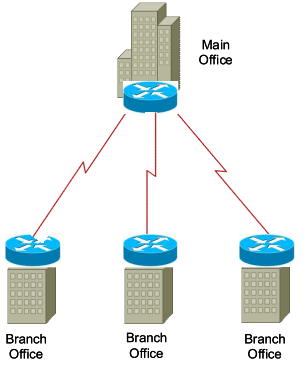
\includegraphics[scale=1]{figures/ex/cmo.png}
\caption{Connection to the Main Office}
\end{figure}

"\`E stata progettata una rete di una piccola compagnia con una topologia gerarchica \textit{Hub-And-Spoke}. La LAN in ogni ufficio secondario è connessa all'ufficio principale tramite un router ed un link con capacità $C = 128\ Kbps$. Dove $(1\ Kbit = 1000\ bits)$. In uno dei siti il flusso del traffico in uscita è generato principalmente da applicazioni CAD fino ad adesso. Per quel traffico, che può essere modellato come un processo di Poisson con rate $\lambda_0 = 3\ pkt/s$, è richiesto che il queueing delay nel router (per i pacchetti in coda) sia meno di $0.5$ secondi con probabilità più grande di $0.99$. A seguito di una nuova configurazione dei processi di business, è anche necessario installare un numero di computer per l'automazione degi uffici. Ci si aspetta che ognuno di loro generi un flusso di pacchetti verso l'ufficio centrale ad un average rate di $\lambda = 1\ pkt/s$. Per quest'ultimo flusso, è richiesto che l'average time speso nel router sia minore od uguale ad 1s.

Le dimensioni dei pacchetti possono essere modellate da variabili casuali indipendenti che sono esponenzialmente distribuite con valore medio $D = 500bytes$.

\begin{itemize}
\item Si assuma che la coda di output del router abbia capacità infinita e sia condivisa da tutti i flussi di traffico secondo disciplina di coda FCFS. Si determini il massimo numero $M$ di nuovi computer che possono essere installati;
\item Considerando il valore $M$, si valuti la \textit{packet loss probability} nel caso la dimensione della coda di output sia limitata a 10 pacchetti.
\end{itemize}

Abbiamo una topologia Hub-And-Spoke. (centro-e-raggi, topologia stellare). $C = 128\ Kbps$. Dove $(1\ Kbit = 1000\ bits) \implies C = 128000\ bit/s$. $\lambda_o = 3\ pkt/s\ \land\ \lambda = 1\ pkt/s$. Si richiede che il ritardo di accodamento nel router sia minore di $0.5s$ con probabilità maggiore di $0.99$. Le lunghezze dei pacchetti sono distribuite esponenzialmente di media 500 bytes. Politica FCFS. Quanto è il numero massimo di computer installabili $M$?

Supponiamo di indicare con $W$ la v.a. che rappresenta il ritardo di accodamento; il vincolo è il seguente, con $(\tau = 0.5s),\ \underline{s=threshold}=0.99$:

\[
	\Pr\{W < (\tau = 0.5s)\ |\ si\ faccia\ coda\} > (0.99 = s)
\]

Indichiamo con $\bar{R}$ il ritardo di accodamento per l'ultimo flusso. Deve valere: $\bar{R} \leq 1s$. Cerchiamo di risolvere il sistema con M/M/1. Abbiamo già delle ipotesi, ma dovremo farne di aggiuntive. Modelliamo quindi il router con un sistema a coda M/M/1:

Abbiamo un buffer output, ed un trasmettitore collegato in serie che è associato al link di uscita. Ipotesi: flusso secondo il quale arrivano i pacchetti di POISSON (pacchetti applicazioni CAD). Stiamo trascurando il ritardo di elaborazione router.
Capacità di elaborazione talmente elevata da ritenersi trascurabile (NO BOTTLENECK). Inoltre: $(d = +\infty)$. Il router opera con FCFS (quella contemplata dal sistema a coda M/M/1). Ipotesi aggiuntiva: certo numero di flussi, $M$ riguardanti i computer dell'Office Automation. Processo degli arrivi di POISSON. Ipotesi di indipendenza abbastanza scontata, dal momento che i vari utenti non si influenzeranno a vicenda. $M\lambda$. Ipotesi aggiuntiva: supponiamo che gli arrivi dei pacchetti relativi ai computer Office Automation siano indipendenti da quelli delle applicazioni CAD. Effettuando il POOLING, abbiamo che la distribuzione risultante è sempre un processo di POISSON con parametro dato dalla somma dei parametri: $\lambda' = \lambda_0+M\lambda$. Quindi $\lambda'$ è la velocità di arrivo dei clienti nel sistema a coda, $\mu$ è la velocità di servizio del router, ovvero il numero medio di pacchetti elaborati dal router per unità di tempo quando il router è costantemente occupato. Abbiamo dei tempi di servizio indipendenti, identicamente distribuiti ed indipendenti dai tempi di interarrivo. Nel sistema i tempi di servizio corrispondono ai tempi di trasmissione. Questo tempo di servizio è legato al parametro (valore medio) $D$ della distribuzione esponenziale che caratterizza la lunghezza dei pacchetti. Quindi abbiamo che il tempo medio di trasmissione è $\frac{1}{\mu} = \frac{D}{C} [s]$, ed abbiamo quindi $\mu = \frac{C}{D} = \frac{1}{D/C} = 32\  [pkt/s]$, ovvero abbiamo 32 pacchetti in media quando il router è costantemente occupato.

\begin{itemize}

\item{\textbf{Parte 1}}

Tutte le ipotesi del sistema a coda M/M/1 sono rispettate. Possiamo quindi utilizzarne i risultati: $\{\lambda',\mu\}$. Dobbiamo andare ad imporre quelle due condizioni. Per un M/M/1, il ritardo per cliente è $\bar{R} = \frac{1}{(\mu-\lambda)}$. Il ritardo per cliente è una v.a. distribuita esponenzialmente $\iff [R \sim EXP(\mu-\lambda)]$. Guardando adesso all'altra condizione, si dimostra che:

\[
	[F_W(y) = \Pr\{W \leq y\} = 1-\rho\e^{-\mu(1-\rho)y},\ y\geq 0]
\]

Tale è la CDF del Ritardo del cliente nella CODA! (Nella sola coda). $W$ sarebbe il tempo di permanenza del cliente nella SOLA coda del sistema a coda M/M/1. Distribuzione valutata su tutti i clienti (anche per quelli che non ci interessano). Dobbiamo condizionarla al fatto che si faccia coda. Quando $(y=0)$, esce $\Pr\{W\leq 0\} = (1-\rho)$. Ovvero la probabilità che il tempo di permanenza in fila di attesa sia nullo è pari a $(1-\rho)$. $\Pr\{W = 0\} = 1-\rho$. Si tratta di una v.a. mista. $\rho$ è il fattore di utilizzazione del router. Nel sistema a coda M/M/1, $\rho = (\frac{\lambda'}{\mu})$. Nell'M/M/1, $(1-\rho)=\pi_0^{(a)}$, ovvero la frazione di tempo a regime nel quale nel sistema a coda non vi sono clienti. La probabilità che il tempo di permanenza sia nullo è PARI alla probabilità che all'arrivo la fila di attesa SIA VUOTA!

\[
	[\Pr\{W = 0\} = 1-\rho = \pi_0]
\]

Questa è pari alla probabilità che un cliente AL SUO ARRIVO vada subito al router. In generale: $\pi_i^{(a)} \neq \pi_i$, laddove il primo membro della disuguaglianza riflette la visione dei clienti all'arrivo, valutata solo sugli istanti di arrivo, mentre il secondo membro riflette la visione all'esterno del sistema, considerando tutto l'asse temporale. $\pi_i$, ponendo l'ERGODICIT\`A, rappresenta la frazione di tempo nel quale vi sono $i$ clienti a regime. Mentre $\pi_i^{(a)}$ è la probabilità calcolata valutando SOLTANTO GLI ISTANTI DI ARRIVO! Frazione degli ARRIVI che trovano il sistema (a regime) nello stato $i$. Infatti potremmo avere ad esempio: $\{\{\pi_1 = \frac{1}{3},\ \pi_0=\frac{2}{3}\}\ \land\ \{\pi_0^{(0)}=1,\ \pi_1^{(0)}=0,\ \pi_2^{(0)}=0\}\}$.

\begin{thrm}{\textbf{P.A.S.T.A. \textit{POISSON ARRIVALS SEE TIME AVERAGES}}}

\[
	\left\{
	\begin{aligned}
	&\pi_i = \lim_{t\to\infty}{\Pr\{N(t)=i\}}\\
	&\pi_i^{(a)} = \lim_{t\to\infty}{\Pr\{N(t)=i\ |\ un\ arrivo\ subito\ dopo\ t\}}
	\end{aligned}
	\right.
\]

Se gli arrivi dei clienti si susseguono con processo di POISSON, abbiamo che: $\pi_i^{(a)}=\pi_i,\ \bar{N}=\sum_{i=0}^\infty{i\pi_i}$

\end{thrm}

Dove la prima equazione è una quantità calcolata sull'insieme delle realizzazioni. (Media di insiemi). Ma se vale L'ERGODICIT\`A, allora le medie d'insieme coincidono con le medie TEMPORALI. $\pi_i$ rappresenta la frazione del tempo nella quale vi sono a regime $i$ clienti nel sistema; $\pi_i^{(a)}$ rappresenta la frazione dei clienti che, all'arrivo trovano il sistema nello stato $i$. Coincide con la probabilità (a regime), che all'arrivo un cliente trovi $i$ clienti nel sistema. Rappresenta cosa vedono i clienti all'arrivo.

Per i nostri scopi, $[\pi_0^{(a)} = \Pr\{W = 0\}] = [\underline{1-\rho = \pi_0}]$, ove la parte sottolineata è la probabilità che vi siano 0 clienti, in un istante qualsiasi, mentre il primo membro è la probabilità che un cliente, al suo arrivo, trovi 0 clienti nel sistema. Grazie al teorema appena visto, esse coincidono. 

$\rho$ è la frazione del tempo in cui il router è occupato $\implies$ probabilità che il router sia occupato. $(1-\rho)$ è la probabilità che il router sia quindi libero. 
$\Pr\{W \leq \tau\ |\ si\ fa\ coda\} = (\dots)$ è la probabilità che il tempo di permanenza in FILA DI ATTESA sia inferiore (od uguale) a $\tau$, quando si fa coda.
Quindi abbiamo:

\[
	(\dots) = 1-\Pr\{W > \tau\ |\ si\ fa\ coda\} = 1-\frac{\Pr\{W > (y := \tau),\ si\ fa\ coda\}}{\Pr\{si\ faccia\ coda\}} = (\dots)
\]

Notiamo che $\{W > y\} \supseteq \{si\ fa\ coda\}$, ed inoltre, dal teorema appena visto (PASTA) vale che: $1-\pi_0^{(a)} = 1-\pi_0 = \rho = \Pr\{si\ fa\ coda\}$, ovvero la probabilità che all'arrivo di un cliente il servitore sia occupato coincide con la probabilità di fare coda. Ciò implica: $\implies$

\[
	(\dots) = 1-\frac{\Pr\{W>\tau\,\ si\ fa\ coda\}}{\Pr\{si\ fa\ coda\}} = 1-\frac{\Pr\{W\geq\tau\}}{\rho} =
\]
\[
	= 1-\frac{\rho\e^{-\mu(1-\frac{\lambda}{\mu})y}}{\rho} = 1-\e^{-\mu(1-\frac{\lambda}{\mu})y},\ y\geq 0
\]

Concludiamo che:

\[
	\Pr\{W \leq y\ |\ si\ fa\ coda\} = 1-\e^{-\mu(1-\frac{\lambda}{\mu})y} \iff W|_{\{si\ fa\ coda\}} \sim EXP(\mu-\lambda)
\]

quindi nell'M/M/1, $R=W|_{\underline{\{si\ fa\ coda\}}}$. Si riferisce proprio alla medesima distribuzione esponenziale, con il medesimo parametro!

Consci che $[R = \frac{1}{\mu-\lambda'}]$, allora procediamo:

\[	
	1-\e^{-(\mu-\lambda')\tau} > s \implies \e^{-(\mu-\lambda')\tau} < (1-s) \implies -(\mu-\lambda')\tau < \log(1-s) \implies (\dots)
\]
\[
	(\dots) \implies -\mu\tau +\lambda'\tau < \log(1-s) \implies [\lambda'\tau < \log(1-s)+\mu\tau] \implies (\dots)
\]
\[
	(\dots) \implies \lambda_0+M\lambda < \frac{\log(1-s)}{\tau} + \mu \implies M\lambda < \mu + \frac{\log(1-s)}{\tau}-\lambda_0 \implies (\dots)
\]
\[
	(\dots) \implies M < \frac{1}{\lambda}[\mu+\frac{1}{\tau}\log(1-s)-\lambda_0] = [32.8]
\]

ove il valore si è ottenuto appositamente sostituendovi i dati al secondo membro dell'ultima disequazione.

Quindi $\floor{M} = M_{max} = 32$ computer massimi.
Si ottiene $M \leq 32.8$, quindi possiamo installare MASSIMO 32 COMPUTER. D'altro canto dobbiamo rispettare anche il vincolo sull'average router time:

\[
	\bar{R} = \frac{1}{\mu-\lambda'} \implies \frac{1}{\mu-\lambda'} \leq 1s \implies ((\mu-\lambda')>0) \geq 1s \implies (\dots)
\]

ove l'ultima parentesizzazione maggiore di 0 indica la condizione di STABILIT\`A, che naturalmente deve essere sempre rispettata.

\[
	(\dots) \implies \mu - (\lambda_0+M\lambda)\geq 1 \implies \mu-\lambda_0 -M\lambda \geq 1 \implies M\leq\frac{\mu-\lambda_0-1}{\lambda} =
\]
\[
	= \frac{1}{\lambda}[\mu-\lambda_0-1] \implies M\leq 28
\]

Ne si conclude che $M_{max}=\min{\{28,32\}} = 28$ computer. Quindi: $\underline{\underline{[M\leq M_{max}=28]}}$.


\newpage

\item{\textbf{Parte 2}}: 

\subsubsection{M/M/1/k}

Consideriamo che $d = 10\ pkt$ (10 pacchetti), $d<+\infty$ ed abbiamo quindi un buffer di dimensione finita. $\iff (d=10)<+\infty$. In questo caso NON possiamo studiare il sistema con un modello M/M/1! Ci serve invece un \textit{M/M/1/k}, nel quale la dimensione del buffer è limitata. Pensiamo a $k$ come la capacità di tutto il sistema (includendo il centro di servizio). Stiamo quindi considerando un sistema a CODA CON PERDITA. Quando un elemento arrivando trova la coda piena, il sistema interviene con il meccanismo di DISCARD (avviene il fenomeno \textit{packet loss}). In questo caso $\lambda'$ è la velocità di arrivo dei clienti al sistema (POISSON). $\lambda_s$ sarà sempre la velocità di ingresso alla coda e di uscita (numero medio di clienti). $\rho=\frac{\lambda_s}{\mu}$ è il fattore di utilizzazione del servitore. Abbiamo che:

\[
	\Pr\{perdita\} = \frac{\lambda^l}{\lambda'} = \pi_k^{(a)} = \pi_k
\]

grazie a PASTA. Disegnamo il relativo DTT della catena:

\begin{center}
\begin{tikzpicture}[->, >=stealth', auto, semithick, node distance=2cm]
\tikzstyle{every state}=[fill=white,draw=black,thick,text=black,scale=1]
\node[state]    (0)                     {$0$};
\node[state]    (1)[right of=0]   {$1$};
\node[state]    (2)[right of=1]   {$2$};
\node[state] (d) [right of=2] {\ldots};
\node[state]    (km1)[right of=d]   {$k-1$};
\node[state]    (k)[right of=km1]   {$k$};
\path
(0) edge[bend left]     node{$\lambda'$}         (1)
(1) edge[bend left]     node{$\lambda'$}         (2)
    edge[bend left,below]    node{$\mu$}            (0)
(2) edge[bend left]     node{$\lambda'$}           (d)
    edge[bend left,below]    node{$\mu$}             (1)
(d) edge[bend left]         node{$\lambda'$}   (km1)
	edge[bend left,below]   node{$\mu$}          (2)
(km1) edge[bend left]       node{$\lambda'$}  (k)
	  edge[bend left,below]   node{$\mu$}     (d)
(k)   edge[bend left,below]  node{$\mu$}          (km1);
\end{tikzpicture}
\end{center}

Sia $N(t)$ il numero di clienti nel sistema a tempo $t$. 
$\Pr\{\phi_i(t) > \tau\} = (\dots)$, dove $\phi_i(t)$ indica il tempo di soggiorno residuo nello stato $i$ al tempo $t$, indica la probabilità che per almeno $\tau$ unità di tempo non ci sia alcun arrivo e NON vi sia la fine del servizio in corso, condizionata con il fatto che attualmente vi sono $i$ clienti nel sistema.

Indichiamo con $\xi_{Rt} \sim EXP(\lambda')$ la v.a. tempo di interarrivo residuo al tempo $t$, e con $\eta_{Rt} \sim EXP(\mu)$ la v.a. tempo di servizio residuo al tempo $t$. Tutte indipendenti ed indipendenti tra di loro, grazie all'ipotesi di (inter)-indipendenza. 

\[
	(\dots) = \Pr\{\xi_{Rt}>\tau,\ \eta_{Rt}>\tau\} = \Pr\{\xi_{Rt}>\tau\}\Pr\{\eta_{Rt}>\tau\} = \e^{-\lambda'\tau}\e^{-\mu\tau} = \e^{-(\lambda'+\mu)\tau}
\]

Quindi abbiamo di nuovo: $-q_{ii} = \mu+\lambda' \implies$

\[
	\tau_{i,i+1} = \frac{q_{i,i+1}}{-q_{ii}} = \frac{q_{i,i+1}}{(\mu+\lambda')}
\]

$\tau_{i,i+1}$ è la probabilità che lasciando lo stato $i$, il processo vada verso $i+1$. Sfruttando il teorema delle probabilità totali nel continuo, abbiamo: $q_{i,i+1} = (\mu+\lambda') \frac{\lambda'}{(\mu+\lambda')} = \lambda'$. Quindi sarà $\lambda'$ fino a $k-1$. La CMTC è una catena omogenea, IRRIDUCIBILE e dal momento che $\cardinality{stati}<+\infty \implies$ allora essa è SICURAMENTE ERGODICA! CATENA SEMPRE ERGODICA. Sistema STABILE.

\[
	\left\{
	\begin{aligned}
	&[\pi_i = \pi_0(\frac{\lambda'}{\mu})^i]\\
	&[\pi_0 = \frac{1}{1+\sum_{i=1}^k{(\frac{\lambda'}{\mu})^i}}]
	\end{aligned}
	\right.
\]

$i=1,2,\ \dots,\ k$.

Notiamo che:

\[
	\sum_{i=0}^k{\rho^i} = \left\{
	\begin{aligned}
	&k+1,\ \rho=1\\
	&\frac{1-\rho^{k+1}}{(1-\rho)},\ p\neq 1
	\end{aligned}
	\right.
\]

Quindi nel nostro caso abbiamo:

\[
	\pi_0 = \frac{1}{\sum_{i=0}^k{\rho^i}} = \frac{1}{\frac{1-\rho^{k+1}}{(1-\rho)}} = \frac{1-\rho}{1-\rho^{k+1}}
\]

Quindi abbiamo come Distribuzione di regime:

\[
	\pi_i = \frac{1-\rho}{1-\rho^{k+1}} \rho^i,\ i=0,1,2,\ \dots,\ k
\]

Si noti che vale anche per $i=0$. Allora:

\[
	[\Pr\{perdita\} = \underline{\pi_k^{(a)} \stackrel{PASTA}{=} \pi_k} = [\frac{1-\rho}{1-\rho^{k+1}} \rho^k]]
\]

da valutarsi con $k=10+1=d+1<+\infty$, in quanto include anche il centro di servizio.
Facendo i calcoli esce $0.07 \implies (70\%)$.

La probabilità di perdita si poteva trovare, come precedentemente enunciato, anche effettuando il rapporto $\frac{\lambda_L}{\lambda'}$. Banalmente, per SPLITTING si ha: $[\lambda_L=\lambda'-\lambda_S]$. Le perdite comunque mi fanno venire meno la caratteristica di POISSON.

\[
	\Pr\{k\ arrivi\ in\ \tau\} = \frac{(\lambda\tau)^k}{k!}\e^{-\lambda\tau}
\]

ma la sequenza degli ingressi a valle della diramazione NON è più di POISSON! $\rho = (\frac{\lambda_S}{\mu})$ rappresenta il fattore di utilizzazione, quindi la frazione del tempo a regime in cui il servitore è occupato. $\rho=1-\pi_0 \implies \pi_0=1-\rho$.

$\lambda_S=\mu(1-\pi_0)$ rappresenta la velocità delle partenze (\textit{departure}) dei clienti dal mio sistema. Abbiamo: $[\pi_0 = \frac{1-\rho}{1-\rho^{k+1}}]$.

\[
	\lambda_L = \lambda'-\lambda_S = \lambda'-\mu(1-\pi_0)
\]

Quindi $\lambda_S$ è la velocità secondo la quale i clienti partono dal sistema, od anche la media dei clienti che partono all'unità di tempo. Guardando il DTT, vi è una partenza quando FINISCE un servizio! Determinando le frequenze delle transizioni a sinistra, potremo sapere le frequenza delle partenze. La frequenza delle partenze si ottiene sommando tutte le frequenze delle transizioni $\pi_iq_{ij}$, sfruttando opportunamente l'inversa della CONDIZIONE DI \underline{NORMALIZZAZIONE}:

\[
	\pi_1\mu + \pi_2\mu +\ (\dots)\ +\pi_k\mu = \mu\sum{\pi_i} = [\lambda_S = \mu(1-\pi_0)]
\]

Stessa cosa mettendoci a valle della diramazione ed a monte della coda: (ARRIVI DI CLIENTI dall'esterno del sistema). $\lambda_S$ rappresenta qui il numero medio di clienti che entrano nel sistema per unità di tempo.

\[
	\lambda_S = [\pi_0\lambda'+\pi_1\lambda'+\ \dots\ +\pi_{k-1}\lambda'] = \lambda'
\]

Valgono le equazioni di bilanciamento locale, valide solo per una CMTC di nascita e morte (BDCMTC):

\[
	\pi_1\mu = \pi_0\lambda' \implies \pi_{k+1}\mu = \pi_k\lambda'
\]

ovvero le sommatorie sono identiche.

$\frac{\lambda_L}{\lambda'}$ rappresenta la probabilità di perdita.

\begin{thrm}{\textbf{Probabilità di perdita}}

\[
	\Pr\{perdita\} = \frac{1-\rho}{1-\rho^{k+1}}\rho^k = \pi_k^{(a)} = \pi_k
\]

ove $\pi_k$ rappresenta la probabilità che il sistema si trovi nello stato $k$ in un istante qualsiasi. Abbiamo anche:

\[
	\Pr\{perdita\} = \frac{(\lambda_L = \lambda'-\lambda_S)}{\lambda'} = 1-\frac{\lambda_S}{\lambda'} = (\dots)
\]
\end{thrm}

Ove $\lambda_S$ è stato trovato applicando Little al primo sottosistema, ottenendo quindi $\lambda_S =\mu(1-\pi_0)$.

\begin{proof}

\[
	(\dots) = 1-\frac{\mu(1-\pi_0)}{\lambda'} = 1-\frac{1}{\rho}(1-\frac{1-\rho}{1-\rho^{k+1}}) = 1-\frac{1}{\rho}(\frac{1-\rho^{k+1}-1+\rho}{1-\rho^{k+1}})
\]
\[
	1-\frac{1}{\rho}\rho \frac{(1-\rho^k)}{(1-\rho^{k+1})} = \frac{1-\rho^{k+1}-1+\rho^k}{1-\rho^{k+1}} = \frac{\rho^k(1-\rho)}{(1-\rho^{k+1})};
\]

\end{proof}

La probabilità di perdita di un cliente deve quindi alla fine coincidere con il rapporto $\frac{\lambda_L}{\lambda'}$.

\end{itemize}

\subsection{Sistemi a coda M/M/m}

Il sistema a coda M/M/m rappresenta una generalizzazione del sistema M/M/1. Abbiamo $m$ router.
Anche in questo caso, il processo degli arrivi è un processo di POISSON con velocità $\lambda$. ($\lambda$ = velocità di arrivo dei clienti). In media arrivano $\lambda$ clienti per unità di tempo. Anche in questo caso i tempi di servizio sono v.a. indipendenti (mutuamente), i.d. con una distribuzione esponenziale negativa unilatera, con tempo medio di servizio $(\frac{1}{\mu})$, ed indipendenti statisticamente dai tempi di interarrivo dei clienti nel sistema a coda. La velocità del centro di servizio sarà variabile (il centro di servizio include ora $m$ servitori), ovvero dipende dal numero di router attivi in un certo istante di tempo. Se $i$ è il numero di clienti nel sistema a coda in un certo istante di tempo, $i<m \implies i\mu$ velocità del centro di servizio. $i$ sono i clienti IN TUTTO IL SISTEMA! In totale quindi i servitori attivi serviranno $i\mu$ utenti $\forall$ unità di tempo. $i\geq m$ tutti gli $m$ servitori saranno attivi $\implies$ velocità $m\mu$. Quindi $i\geq m$ centro di servizio alla massima velocità possibile. $m\mu$ = capacità TOTALE DI SERVIZIO DEL SISTEMA (del centro di servizio). Come nella M/M/1, la dimensione del buffer e la popolazione sono illimitate ($\iff d,e<+\infty$). Disciplina di queueing di default (FCFS). Modellabile come uno stack FIFO. Se arriva un cliente e c'è un certo numero di router liberi, sarà assegnato in maniera random ad uno di questo. Approccio MARKOVIANO basato sul processo stocastico che si riferisce al numero di clienti nell'intero sistema a coda al tempo $t$, ovvero $N(t)$. La sua evoluzione sarà determinata dalle v.a. tempi di interarrivo e tempi di servizio. Dato che per queste ipotesi queste v.a. sono prive di memoria e statisticamente indipendenti $\implies$ siamo dinanzi una CMTC, il cui diagramma dei tassi di transizione è il seguente:

\begin{center}
\begin{tikzpicture}[->, >=stealth', auto, semithick, node distance=2cm]
\tikzstyle{every state}=[fill=white,draw=black,thick,text=black,scale=0.8]
\node[state]    (0)                     {$0$};
\node[state]    (1)[right of=0]   {$1$};
\node[state]    (2)[right of=1]   {$2$};
\node[state] (d) [right of=2] {\ldots};
\node[state]    (mm1)[right of=d]   {$m-1$};
\node[state]    (m)[right of=mm1]   {$m$};
\node[state]    (mp1)[right of=m]   {$m+1$};
\node[state]    (mp2)[right of=mp1]   {$m+2$};
\node[state]    (d2)[right of=mp2]  {\ldots};

\path
(0) edge[bend left]     node{$\lambda$}         (1)
(1) edge[bend left]     node{$\lambda$}         (2)
    edge[bend left,below]    node{$\mu$}            (0)
(2) edge[bend left]     node{$\lambda$}           (d)
    edge[bend left,below]    node{$2\mu$}             (1)
(d) edge[bend left]         node{$\lambda$}   (mm1)
	edge[bend left,below]   node{$3\mu$}          (2)
(mm1) edge[bend left]       node{$\lambda$}  (m)
	  edge[bend left,below]   node{$(m-1)\mu$}     (d)
(m)   edge[bend left]   node{$\lambda$}      (mp1)
      edge[bend left,below]  node{$m\mu$}          (mm1)
(mp1) edge[bend left]       node{$\lambda$}  (mp2)
	 edge[bend left,below]   node{$m\mu$}      (m)
(mp2) edge[bend left]       node{$\lambda$}   (d2)
      edge[bend left,below] node{$m\mu$}    (mp1)
(d2) edge[bend left,below]   node{$m\mu$}     (mp2);
\end{tikzpicture}
\end{center}

CMTC nascita e morte (BDCMTC), con $\cardinality{stati}=+\infty$ (infiniti), fila di attesa di dimensione illimitata. Tassi di nascita pari a $\lambda$, tassi di morte $m\mu$, che sarebbe il tasso di morte nello stato $i$ prima che si saturino i servitori disponibili, dopodiché $(i\geq m)$, sempre pari a $m\mu$.

\subsubsection{Calcolo dei tassi (velocità) di transizione}

Supponiamo $N(t)=i\neq 0$ ($i$ clienti nel mio intero sistema a coda), ovvero qualsiasi stato diverso dallo stato banale. Il successivo cambiamento di stato sarà legato od all'arrivo di un nuovo cliente od al completamento di uno dei servizi eseguiti in parallelo al tempo $t$. Comunque abbiamo $i$ clienti totali. Possibili casi: $\{i++,\ i--\}$. L'intervallo di tempo da $t$ al successivo arrivo lo indichiamo con $\underline{\xi_R(t) \sim EXP(\lambda)}$, ovvero il tempo di interarrivo residuo (stessa caratteristiche dei tempi di interarrivo). Il tempo che passa tra l'istante presente $t$ ed il successivo completamento del servizio, sarà $\eta_R(t)$, e sarà pari al minimo dei tempi di servizio residui in $t$. Ci saranno un certo numero di servizi. $\eta_R(t) = \min{\{...\}}$, ovvero al minimo dei tempi di servizio residui legati a quei servizi che al tempo $t$ stanno procedendo in parallelo. Quando $i<m$, ci saranno $i$ servizi che stanno procedendo in parallelo. Anche i tempi di servizio residui sono \underline{indipendenti} fra di loro per ipotesi, dal momento che i servizi procedono in parallelo senza influirsi. Quindi $\eta_R(t) \sim EXP(\sum_i{\mu_i})$. Quando $i<m\implies$ $\eta_R(t) \sim EXP(i\mu)$. Se invece $i\geq m$, $\eta_R(t) \sim EXP(m\mu)$. A questo punto, il tempo che passa dall'istante presente $t$ e la successiva transizione di stato, sarà $\phi_i(t)$ (tempo di soggiorno residuo nello stato $i$ al tempo $t$) prima di cambiare stato $\implies$

\[
	\phi_i(t) = \min{\{\xi_R(t),\ \eta_R(t)\}} \implies \phi_i(t) \sim EXP(-q_{ii})
\]

ove l'ultima implicazione è valida grazie al fatto che queste variabili casuali sono i.i.d. ed indipendenti tra di loro. Abbiamo:

\[
	-q_{ii} = \left\{
	\begin{aligned}
	&(\lambda+i\mu),\ i<m\\
	&(\lambda+m\mu),\ i\geq m
	\end{aligned}
	\right.
\]

(Velocità totale di uscita \underline{dallo stato i}). Parametro $-q_{ii}$. Quindi, quella quantità rappresenta con che velocità in totale esco dallo stato. Ma se $\underline{i<m}$, perché $q_{i,i+1} = \lambda,\ q_{i,i-1}=i\mu$. Solito giochetto. (Se $i\geq m,\ q_{i,i-1}=m\mu$). Consideriamo:

\[
	\tau_{i,i+1} = \frac{q_{i,i+1}}{-q_{ii}} = \Pr\{\xi_R(t) < \eta_R(t)\} = (\dots)
\]

ove l'ultima quantità rappresenta la probabilità che il prossimo arrivo preceda la fine del servizio (il completamento del servizio). Dobbiamo quindi applicare il teorema delle probabilità totali nel continuo, ottenendo alla fine:

\[
	(\dots) = \left\{
	\begin{aligned}
	&\frac{\lambda}{\lambda+i\mu},\ i<m\\
	&\frac{\lambda}{\lambda+m\mu},\ i\geq m
	\end{aligned}
	\right.
\]

CMTC OMOGENEA, IRRIDUCIBILE, ma non sappiamo tuttavia se è ERGODICA.

\[
	\left\{
	\begin{aligned}
	&[\pi_0 = \frac{1}{1+\sum_{i=1}^{m-1}{(\frac{\lambda}{\mu})^i\frac{1}{i!}} + (\frac{m^m}{m!})\sum_{i=m}^\infty{(\frac{\lambda}{m\mu})^i}}]\\
	&\left\{
	\begin{aligned}
	&\pi_i = \pi_0 (\frac{\lambda}{\mu})^i \frac{1}{i!},\ i<m\\
	&\pi_i = \pi_0 (\frac{\lambda}{\mu})^i \frac{1}{m!m^{i-m}},\ i\geq m
	\end{aligned}
	\right.
	\end{aligned}
	\right.
\]

Dobbiamo capire qual'è la CONDIZIONE MAX di ERGODICIT\`A (si ha una condizione di regime). La sommatoria ad infiniti termini (serie) a denominatore di $\pi_0$ deve convergere di nuovo. La condizione di ERGODICIT\`A è quindi: $(\frac{\lambda}{m\mu}) < 1$ (convergenza della serie geometrica). Quando $\rho := \frac{\lambda}{m\mu} < 1$ questa sommatoria (serie) converge, e si ha una distribuzione che è quella di regime. $[\lambda < m\mu]$ è proprio la condizione di STABILIT\`A, la quale indica che la velocità di arrivo deve essere minore della capacità totale di servizio. Serve sostanzialmente per evitare l'"ingolfamento". $\rho$ è il fattore di utilizzazione del generico router (Non del centro di servizio). Ognuno dei router avrà un fattore di utilizzazione pari a $\rho$, quando il carico è EQUAMENTE DISTRIBUITO. $\frac{\lambda}{m}$ sarà la capacità di arrivo del singolo cliente. Servono in media lo stesso numero di clienti $\forall$ unità di tempo. Tutti lavoreranno alla stessa maniera. Ogni router si vedrà arrivare quindi $\frac{\lambda}{m}$ clienti per unità di tempo. Fattore di utilizzazione; frazione di tempo quando il servitore è occupato. Infatti, applicando \underline{Little} troviamo: $(\frac{\lambda}{m})(\frac{1}{\mu})$, trovando la frazione di tempo nel quale il router è occupato per unità di tempo nella quale il router è costantemente occupato, quando il carico di lavoro è EQUAMENTE DISTRIBUITO. $\frac{\lambda}{\mu}$ è l'\textit{intensità di traffico} (arrivano $\lambda$ clienti, $\frac{1}{\mu}$ è il lavoro medio richiesto dal cliente). Quindi sfruttiamo ancora Little e troviamo: $\lambda(\frac{1}{\mu})$, trovando così il \underline{\underline{CARICO MEDIO DI LAVORO}}. 

\[	
	[\frac{\lambda}{\mu} = m(\rho := \frac{\lambda}{m\mu}) = m\rho]
\]

Si usi questo fatto per vedere a cosa converge la sommatoria geometrica:

\[	
	[\pi_0 = \frac{1}{\sum_{i=0}^{m-1}{(m\rho)^i \frac{1}{i!}} + (\frac{m^m}{m!} \frac{\rho^m}{1-\rho} = \frac{(m\rho)^m}{m!(1-\rho)})}]
\]

e tramite questa espressione possiamo ovviamente trovare le $\pi_i$.

ERGODICIT\`A se: $[\underline{\lambda < m\mu}]$. Abbiamo trovato la distribuzione di regime. Nel caso M/M/1, abbiamo poi ricavato tutti i numeri medi di clienti e tempi di servizio, etc. Nel caso M/M/1 siamo partiti da $\bar{N}$.

\subsubsection{Quantità medie tipiche}

Adesso partiamo da $\bar{T}$, ovvero il ritardo medio per cliente a regime. Terminologia tempo di risposta. $\bar{T}$ tempo di risposta. Tempo di permanenza del cliente nel sistema a coda. Abbiamo:

\[
	(\bar{T} := \E[T]) = \E[t_s] + \E[W] = \frac{1}{\mu} + (\dots)
\]

ove $W$ è il tempo di accodamento, ovvero il queueing delay. Adesso per valutare il tempo medio di permanenza in fila di attesa utilizziamo il concetto di \textit{MEDIA CONDIZIONATA}:

\[
	(\dots) = \E[\E[W\ |\ k\ clienti\ all'arrivo]] = \mathord{\cdot}(k)
\]

dove $\{k\ clienti\ all'arrivo\}$ sarebbe l'evento nel quale troviamo $k$ clienti all'arrivo in testa al sistema. Tempo di permanenza, sapendo che all'arrivo il cliente trova $k$ clienti nel sistema. Quindi:

\[
	\bar{T} = \frac{1}{\mu} + \sum_{k=m}^\infty{\E[W\ |\ k\ clienti\ all'arrivo]}\pi_k^{(a)}
\]

Notiamo che $k$ parte da $m$, perché se $k<m$ quella quantità sarebbe nulla!
Il tempo medio di permanenza nella fila di attesa è nullo quindi se $k<m$! Se arrivato nel sistema a coda trovo un numero $(k<m)$ di clienti, allora VADO DIRETTAMENTE nel CENTRO DI SERVIZIO! Sommatoria che parte da $m$ quindi. Volendo la si potrebbe fare partire da 0, senza alcuna perdità di generalità, dal momento che i primi $(m-1)$ termini sarebbero comunque nulli. Abbiamo:

\[	
	\bar{T} = \frac{1}{\mu} + \sum_{k=m}^\infty{\frac{k-m+1}{m\mu}(\pi_k^{(a)}=\pi_k)} = (\dots)
\]

Dove l'uguaglianza tra parentesi deriva da PASTA. Abbiamo sfruttato il fatto che: $[\E[W|k] = \frac{k-m+1}{m\mu}]$. Siamo nel caso $k\geq m$, ove vi sono $m$ clienti al servizio, $(k-m)$ clienti in fila di attesa ed io. Dopo che vi sarà il completamento di $(k-m)$ servizi mi troverò in testa alla fila di attesa. Ma dovrò quindi attendere il completamento di un ulteriore servizio (ecco perché il termine $+1$). Ma il tempo tra il completamento del servizio corrente ed il successivo è $(\frac{1}{m\mu})$! ($\leftarrow$ tempo medio di servizio). $\implies$

\[
	(\dots) = \frac{1}{\mu} + \sum_{k=m}^\infty{(\frac{k-m+1}{m\mu})\pi_0\frac{m^m}{m!}\rho^k} = \frac{1}{\mu} + \pi_0\frac{m^m}{m!}\sum_{k=m}^\infty{\frac{k-m+1}{m\mu}\rho^k} = (\dots)
\]

A questo punto possiamo porre: $i := k-m+1$, ed otteniamo:

\[
	(\dots) = \frac{1}{\mu} + \pi_0\frac{m^m}{m!m\mu}\sum_{i=1}^\infty{i(\rho^{i-1+m} = \rho^{i-1}\rho^m)} =
\]
\[
	= \frac{1}{\mu} + \frac{(m\rho)^m}{m!m\mu}\pi_0\sum_{i=1}^\infty{i\rho^{i-1}} = [\frac{1}{\mu} + \frac{\pi_0(m\rho)^m}{m!m\mu} \frac{1}{(1-\rho)^2}]
\]

Abbiamo quindi trovato il RITARDO MEDIO PER CLIENTE. Volendo potremmo anche trovare con Little: $\bar{N}=\lambda\bar{T} = (\dots)$. Spesso in letteratura si esprime $\bar{T}$ in funzione della probabilità di attesa:

\[
	\Pr\{accodamento\ (queueing)\} = \sum_{k=m}^\infty{(\pi_k^{(a)}=\pi_k)}
\]

sarebbe ovvero la sommatoria di queste probabilità. Si deriva quindi la \textit{C di ERLANG}. (La B di ERLANG è invece collegata alla probabilità di perdita (M/M/m/0)). 

Siamo in un sistema a coda M/M/m. Ritardo medio per cliente:

\[
	\left\{
	\begin{aligned}
	&\bar{T} = \frac{1}{\mu} + \frac{\pi_0(m\rho)^m}{m!m\mu} \frac{1}{(1-\rho)^2}\\
	&\rho = \frac{\lambda}{m\mu},\ \rho<1
	\end{aligned}
	\right.
\]

ove l'ultima equazione del sistema indica la condizione di \underline{STABILIT\`A}. Questa quantità ($\bar{T}$), viene solitamente espressa in letteratura in funzione della probabilità di ATTESA, nella quale dobbiamo considerare la situazione in cui abbiamo almeno $m$ clienti nel sistema a coda quando arriva un cliente:

\[
	\Pr\{queueing\} = \sum_{k=m}^\infty{(\pi_k^{(a)}=\pi_k)} = \sum_{k=m}^\infty{\pi_k} =
\]
\[
	\sum_{k=m}^\infty{\pi_0(\frac{\lambda}{m\mu} = \rho)^k \frac{m^m}{m!}} = \pi_0\frac{m^m}{m!}\sum_{k=m}^\infty{\rho^k} = (\dots)
\]

Siamo dinanzi una sommatoria geometrica, quindi:

\[
	(\dots) = \pi_0\frac{m^m}{m!} (\frac{\rho^m}{1-\rho}) = \frac{\pi_0(m\rho)^m}{m!(1-\rho)} := C(m,\frac{\lambda}{\mu})
\]

Abbiamo ottenuto quest'espressione $C(m,(\frac{\lambda}{\mu}))$, nota come funzione \textit{C di ERLANG} con parametro: $\{m,(\frac{\lambda}{\mu})\}$. Ci sono delle tabelle per questa formula. Abbiamo ricavato un modello per la M/M/m. Possono essere utilizzate per modellare quei sistemi di servizio che prevedono diverse risorse. Sistemi di servizio con un certo numero di risorse, corrispondenti ai router $(m)$, laddove $(i\geq m \implies\ queueing)$.

Modello M/M/m. Dobbiamo però ritrovare le ipotesi dietro all'M/M/m nel mondo reale. Call-center ad esempio. Processo secondo il quale si susseguono gli arrivi al sistema a coda dev'essere ben modellabile come un processo di POISSON. Durata media delle telefonate (tempi medi di servizio) $(\frac{1}{\mu})$. In un call center mi ritrovo queste ipotesi. Ci vorrebbero anche le ipotesi sulla dimensione del buffer e della popolazione. $(d,e = +\infty)$. Dimensionamento del numero massimo di operatori (servitori) in base ad un predeterminato massimo valore da non scavalcare relativo alla probabilità di accodamento. $\{\lambda,\frac{1}{\mu}\} \to m$. Problema di progetto. Potremo anche voler affrontare un problema di ANALISI. Durata media delle telefonate $(\frac{1}{\mu})$. [ANALISI $\rightarrow$ PROGETTO]. In funzione della C di ERLANG, troviamo il valore del ritardo medio per cliente:

\[
	\bar{T} = \frac{1}{\mu} + C\frac{1}{m\mu}(\frac{1}{1-\rho}),\ \rho<1
\]

Ricordiamo che $(C\ di\ ERLANG = \Pr\{queuing\})$. Adesso, noto il valore del ritardo medio per cliente, applico Little e trovo:

\[
	\bar{N} = \lambda\bar{T} = \frac{\lambda}{\mu} + C\frac{\lambda}{m\mu}(\frac{1}{1-\rho}) = [m\rho + C\rho(\frac{1}{1-\rho})]
\]

Troviamo ora il tempo medio di permanenza nella sola fila di attesa, dove $(\rho := \frac{\lambda}{m\mu})$:

\[
	\bar{W} = \bar{T} - (T_s = \frac{1}{\mu}) = C\frac{1}{m\mu}(\frac{1}{1-\rho})
\]

E adesso il numero medio di clienti nella sola fila di attesa, $\bar{N_q}$

\[
	[\bar{N_q} = \lambda\bar{W} = C\rho(\frac{1}{1-\rho})]
\]

Dove abbiamo nuovamente applicato Little al sottosistema costituito dalla sola fila di attesa. Ora passiamo al centro di servizio, ragionando con gli stessi argomenti:

\[
	\left\{
	\begin{aligned}
	&(T_s=\frac{1}{\mu})\\
	&\bar{N_s} = m\rho := \frac{\lambda}{\mu} = \lambda(\frac{1}{\mu})
	\end{aligned}
	\right.
\]

$\rho$ è il FATTORE DI UTILIZZAZIONE. A REGIME $(\rho<1)$. Ricordiamo che $\lambda$ è sempre la velocità di arrivo.

\subsubsection{Confronto tra tre sistemi MARKOVIANI}

Questi tre sistemi MARKOVIANI hanno la stessa capacità di servizio e stessa velocità tutti tra di loro:

\begin{itemize}

\item{1)}: Un singolo sistema M/M/1 con velocità di arrivo $m\lambda$ e velocità di servizio del singolo servitore pari a $m\mu$. Parametri: $\{m\lambda,m\mu\}$;
\item{2)}: $m$ code M/M/1, ogni coda con velocità di arrivo $\lambda$ e di servizio $\mu \implies\ \{m\lambda,m\mu\}$ come parametri;
\item{3)} Sistema M/M/m con velocità di arrivo $m\lambda$ ed $m$ servitori. Ricordiamo che qui vale:

\[
	[\frac{1}{\mu} + C\frac{1}{m\mu}(\frac{1}{1-\rho}) = \bar{T},\ (\rho<1)]
\]

Abbiamo parametri: $\{m\lambda,m\mu\}$.

\end{itemize}

Tre sistemi che hanno tutti la stessa velocità di arrivo e di servizio. Confrontiamo i ritardi medi di permanenza per i clienti. Dobbiamo quindi stilare una graduatoria:
Effettuiamo un confronto:

\[
	\left\{
	\begin{aligned}
	&\bar{T_1} = \frac{1}{m\mu-m\lambda} = \frac{1}{m(\mu-\lambda)}\\
	&\bar{T_2} = \frac{1}{\mu-\lambda}\\
	&\bar{T_3} = ?
	\end{aligned}
	\right.
\]

Dovremmo fare i conti con l'espressione di $\bar{T}$ precedentemente trovata. Ma, intuitivamente la classifica sarebbe: $\{1,3,2\}$. Il primo sarebbe il migliore, sebbene poco attuabile nella pratica. Ci accontentiamo del terzo sistema. Primo sistema non attuabile come umani come router. Il primo lavora sempre alla capacità di servizio, mentre il terzo ha capacità di servizio $m\mu$ solo quando $i\geq m$!

\subsubsection{M/M/m/0}

In questo sistema abbiamo 0 come dimensione del buffer \newline
$\iff (d=0)<+\infty$. \underline{\underline{NO POISSON modeling}}!
In letteratura troviamo anche M/M/m/m $(d=m)$. Nel primo caso con $d$ si intende la dimensione del buffer, mentre $(d=m)$ intende il numero totale di clienti nel sistema. Ovviamente M/M/m/0 $\neq$ M/M/m, in quanto se $i\geq m$, i clienti in arrivo vengono irrimediabilmente persi. $m$ router e velocità $\mu$ ciascuno $(\frac{1}{\mu})$ ritardo medio per cliente. v.a. memoryless EXP (UNI-NEG). statisticamente indipendenti i.d. ed indipendenti statisticamente dai tempi di interarrivo (MARKOV). $\lambda_D=\lambda_S$, dove $D$ sta per \textit{departure}. Si può verificare quindi il fenomeno di \underline{LOSS}. Sistema con blocco, ma con \underline{perdita} (Non si può fare fila in coda). $\lambda_S$ sarà anche la velocità di partenza! Le perdite fanno perdere la proprietà di POISSON per il processo che modella il numero di clienti. Di conseguenza il processo secondo il quale entrano i clienti nel centro di servizio NON è più di POISSON, il quale modellerebbe la distribuzione di massa in tal modo:

\[	
	\Pr\{k\ arrivi\ in\ \tau\} = \frac{(\lambda\tau)^k}{k!}\e^{-\lambda\tau}
\]

Ma in questo caso è 0 se $k\geq m$! $N(t)$ è il numero di clienti nel sistema a coda al tempo $t$. Sostanzialmente coincide con il numero di clienti nel centro di servizio del sistema. $\underline{\underline{N(t)}}$. Sia una CMTC, dal momento che abbiamo indipendenza tra $\lambda$ e $\mu$. Il diagramma DTT è il seguente:

\begin{center}
\begin{tikzpicture}[->, >=stealth', auto, semithick, node distance=2.3cm]
\tikzstyle{every state}=[fill=white,draw=black,thick,text=black,scale=1]
\node[state]    (0)                     {$0$};
\node[state]    (1)[right of=0]   {$1$};
\node[state]    (2)[right of=1]   {$2$};
\node[state]    (3)[right of=2]   {$3$};
\node[state] (d) [right of=3] {\ldots};
\node[state]    (mm1)[right of=d]   {$m-1$};
\node[state]    (m)[right of=mm1]   {$m$};

\path
(0) edge[bend left]     node{$\lambda$}         (1)
(1) edge[bend left]     node{$\lambda$}         (2)
    edge[bend left,below]    node{$\mu$}            (0)
(2) edge[bend left]     node{$\lambda$}           (3)
    edge[bend left,below]    node{$2\mu$}             (1)
(3) edge[bend left]     node{$\lambda$}           (d)
    edge[bend left,below]    node{$3\mu$}             (2)
(d) edge[bend left]         node{$\lambda$}   (mm1)
	edge[bend left,below]   node{$3\mu$}          (3)
(mm1) edge[bend left]       node{$\lambda$}  (m)
	  edge[bend left,below]   node{$(m-1)\mu$}     (d)
(m)   edge[bend left,below]  node{$m\mu$}          (mm1);
\end{tikzpicture}
\end{center}

Mi trovo dinanzi ad una catena di nascita e morte (BDCMTC) con insieme degli stati FINITO $(\iff \cardinality{stati}<+\infty)$. Abbiamo i seguenti tassi di transizione, trovati rispetto al DTT relativi all'M/M/m (lì avevamo però un numero di stati infinito):

\[
	\left\{
	\begin{aligned}
	&\lambda_i=\lambda\ \forall i=0,1,\ \dots,\ m-1\\
	&\mu_i = i\mu,\ i=1,\ \dots,\ m
	\end{aligned}
	\right.
\]

ove l'ultimo range di indici relativo al tassi di morte è tale per cui sarebbe 0 altrimenti. La catena è ERGODICA $\iff$ esiste sicuramente la distribuzione di regime:

\[
	\left\{
	\begin{aligned}
	&[\pi_i = \pi_0 (\frac{\lambda}{\mu})^i (\frac{1}{i!})],\ i=1,\ \dots, m\\
	&[[\pi_0 = \frac{1}{1+\sum_{k=1}^m{(\frac{\lambda}{\mu})^k (\frac{1}{k!})}}] = \frac{1}{\underline{\sum_{k=0}^m{(\frac{\lambda}{\mu})^k (\frac{1}{k!})}}}]
	\end{aligned}
	\right.
\]

ove nell'ultimo passaggio sottolineato dell'equazione abbiamo inglobato l'1 nella sommatoria. Ora sappiamo già che è ERGODICA (la sommatoria è una semplice SOMMA di un numero finito di elementi, quindi convergerà sicuramente).

\[
	[\pi_i = \frac{(\frac{\lambda}{\mu})^i (\frac{1}{i!})}{\sum_{k=0}^m{(\frac{\lambda}{\mu})^k (\frac{1}{k!})}}]
\]

$\leftarrow$ ovvero la probabilità di regime, per $\underline{0\leq i\leq m}$. Quando $(i=0)$, trovo esattamente $\pi_0$ in evidenza.

$\bar{N}$ sia il numero medio di clienti nel sistema. $\implies \bar{N}=\sum_{i=0}^m{i\pi_i}$. Possiamo applicare anche Little al centro di servizio: $\implies \bar{N}=\lambda_S(\frac{1}{\mu})$. Abbiamo:

\[
	[\lambda_S = \sum_{i=0}^{m-1}{\lambda\pi_i}] = \underline{\lambda(1-\pi_m)} =
\]
\[
	= [\lambda\pi_0 + \lambda\pi_1 + \lambda\pi_2+\ \dots+\ \lambda\pi_{m-1}]
\]

dove il termine sottolineato si riferisce alla NORMALIZZAZIONE (per via della condizione di NORMALIZZAZIONE). Stiamo sostanzialmente sommando le frequenze di transizione, considerando quelle transizioni che si riferiscono all'evento $\{entra\ un\ cliente\ nel\ mio\ sistema\}$. Sommatoria delle frequenze. Ogni qualvolta vi è una transizione, significa che è arrivato un cliente che è entrato nel centro di servizio. Per trovare il numero medio di clienti che entrano nel mio sistema a coda, basta sommare le frequenze di queste transizioni. Ad un certo punto, i clienti se ne escono $\implies [\lambda_D=\lambda_S]$. Potremo effettuare lo stesso ragionamento:

\[
	\pi_1\mu + \pi_2(2\mu) + \pi_3(3\mu) +\ \dots+\ \pi_m(m\mu) = \lambda_D = \lambda_S
\]

Ad esempio $\pi_1\mu$ rappresenta il numero medio di volte che accade questo evento di interesse per unità di volte o frequenze di transizioni. $\pi_iq_{ij}$ è anche chiamato flusso, FLUSSO dallo stato $i$ allo stato $j$. Frequenza di transizione. $\{\pi_jq_{ji},\pi_iq_{ij}\}\ |\ \pi_1\mu = \pi_0\lambda$. Quest'ultima quantità rappresenta quante volte in media un cliente all'arrivo trova 0 clienti. Queste sono le cosiddette equazioni di bilanciamento locale, e sono valide solo per una CMTC nascita e morte. Ad esempio: $[\pi_1\mu = \pi_0\lambda],\ \pi_{m-1}\lambda = \underline{\pi_m m\mu}$, ovvero la frequenza con la quale un cliente arriva e si becca l'unico router disponibile.

Una importante quantità è la cosiddetta probabilità di perdita (legata alla B di ERLANG).

\[
	\Pr\{LOSS\} = \underline{\pi_m^{(a)} = \pi_m} = \frac{{(\frac{\lambda}{\mu})^m \frac{1}{m!}}}{\sum_{i=0}^m{(\frac{\lambda}{\mu})^i (\frac{1}{i!})}} = B(m,\ \frac{\lambda}{\mu})
\]

Tale quantità è la \underline{B di ERLANG con parametri $m,\ \frac{\lambda}{\mu}$}. Ancora più importante della prima. Con questa formula sono state dimensionate opportunamente le centrali telefoniche. Certe quantità di servizi ma NON è possibile fare fila di attesa nel caso in cui $i\geq m$. Per un call center NON si potrebbe utilizzare ovviamente. Si dimostra che quanto scritto, vale per il sistema \textbf{M/G/m/0}, in generale, ovvero anche quando abbiamo una distribuzione arbitraria dei tempi di servizio.

\subsubsection{Typical scenario}

Fino a poco tempo fa i RAS erano dei router con delle porte seriali alle quali si collegavano i modem (\underline{SLIP}). Il computer chiedeva al modem di collegarsi ad un altro utente, ed era necessario che ci fosse ovviamente un'interfaccia libera. Ad ogni borchia era associato un numero di telefono. Allora le applicazioni non richiedevano tutta questa banda.

Circuiti telefonici tra un modem ed un altro modem. PPP = \textit{Point to Point Protocol}. Tramite PPP venivano inoltrati i vari pacchetti IP. Questo sistema può essere studiato con un M/M/m/0. Ipotesi da fare nel sistema reale. I clienti arrivano con un processo di POISSON a velocità $\lambda$. $m$ porte corrispondenti agli $m$ router. I circuiti telefonici non si creerebbero se $i\geq m$. Perdita. Le richieste di chiamata si devono susseguire in un modo tale da essere ben modellate con un processo di POISSON. Velocità medie delle richieste. I tempi di servizio dovevano essere v.a. i.i.d. (EXP-UNINEG). $(\frac{1}{\mu})$. Qui i tempi di servizio sono i tempi di collegamento. Anche indipendenti dai tempi di interarrivo, ovviamente. M/G/m/0. Anche se non fossero (EXP-UNINEG), funzionerebbero lo stesso per questo tipo di sistema, difatti quanto un utente sta collegato, non influenza i vari tempi. 

Posso effettuare un problema di progetto. Dati $\lambda,\ \frac{1}{\mu}$, ove l'ultimo parametro rappresenta la durata media dei tempi di collegamento, dobbiamo risolvere il seguente problema:

\[
	\min{m}\ |\ \Pr\{LOSS\} < \underline{S}
\]

ove la quantità sottolineata è un'apposita threshold. \`E interesse del provider che il suo sistema funzioni bene. Si utilizzi la B di ERLANG $(B(m,\frac{\lambda}{\mu}))$. Se $B$ è elevata, dobbiamo evidentemente aumentare $m\ \iff m\uparrow$, e pensare ad un problema di PROGETTO.

Con l'ADSL si utilizza l'ATM (dimensionamento del sistema). L'\textit{Access Concentrator} è un router del provider collegato mediante interfaccia ATM alla rete ATM. Varie possibilità di PPP: \{PPPoA, PPPoE\}. [DSLAM = \textit{Digital Subscriber Link Access Multiplexer}]. Multiplatore dell'accesso da parte di linee che giungono da diversi clienti. Dal router ADSL ci si collega sino al DSLAM, che si trova in centrali, mediante DOPPINO. Nel caso PPPoA, il PPP agisce tra i due estremi (router ADSL ed Access Concentrator). Il DSLAM è come se fosse uno switch ATM. Ricordiamo lo stack: $\{IP \to PPP \to AAL5 \to PHY\}$. Il PPP è poggiato sull'ATM. Attraverso le celle ATM, il pacchetto giungerà all'Access Concentrator e verrà adeguatamente deimbustato. Con il PPPoE, la sessione PPP è tra il mio computer e l'Access Concentrator. IN TAL CASO NON SI COMPORTANO PIU' COME ROUTER! Access Concentrator ed il primo router fanno da BRIDGE REMOTI! In tal caso lo stack sarebbe: $\{IP \to PPP \to Eth. \to PHY\}$. Pacchetto IP imbustato in PPP a livello di computer. La trama Ethernet, quando arriva al router bridge, tramite le celle ATM viaggerà e verrà alla fine deimbustato (all'altra estremità del circuito virtuale). L'Access Concentrator ovviamente avrà m router.

\subsubsection{Exercise}

Si debba progettare un servizio di accesso remoto basato su VPN IPSec di cui possano usufruire i dipendenti di un'azienda.

Si assuma che le richieste di instaurazione di una VPN arrivino secondo un processo di Poisson a velocità $\lambda=200\ req/s$ e che le connessioni sicure durino in media $\frac{1}{\mu} = 30\ min$. Determinare il numero minimo $\mathbf{m}$ di VPN contemporanee che il concentratore di VPN deve essere in grado di supportare affinché la probabilità di rifiuto di una richiesta in arrivo sia minore di $S=0.01$.

Il candidato introduca le eventuali ulteriori ipotesi necessarie al fine di poter utilizzare il modello stocastico che intende adottare per la progettazione.

\begin{center}
\begin{figure}[H]
\centering
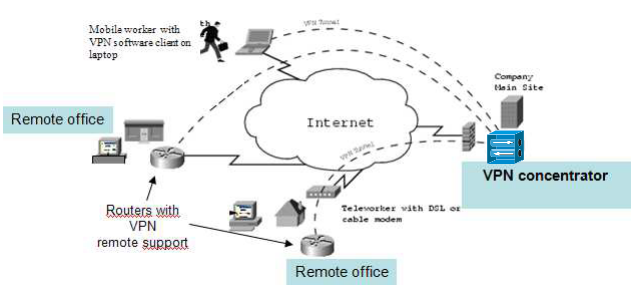
\includegraphics[scale=0.8]{figures/ex/VPN.png}
\caption{VPN IPSec}
\end{figure}
\end{center}

Risoluzione:

$S=0.01$. VPN IPSec. Accesso da remoto ad Internet e si basa sulla presenza di un \textit{VPN Concentrator} (concentratore di reti virtuali). IPSec, SSL. Meccanismi di sicurezza. Concentratore tramite VPN. Un router normale ne supporta fino ad una centinaia di VPN (Grandi aziende come CISCO, IBM). Le richieste di instaurazione arrivano secondo un processo di POISSON. $\lambda = 200\ req/h$. Inoltre $\frac{1}{\mu} = 30\ min$ (tempo medio di servizio). $m=?\ |\ \Pr\{LOSS\} < (S = 0.01)$.

M/M/m/0. Il processo degli arrivi di POISSON. Ci viene chiesto il numero di VPN contemporanee da supportare. Sistema con PERDITA (LOSS). ed ipotesi standard sui vari tempi. $m$ router. $m$ numero di VPN contemporanee. FCFS come disciplina di coda. Non c'è una coda però, quindi non conta tanto. $(\iff d=0, (e=+\infty))$.

Vogliamo utilizzare le tabelle (B di ERLANG). Il \underline{CARICO MEDIO di LAVORO} (INTENSIT\`A DI TRAFFICO) è $(\frac{\lambda}{\mu}) = (200 x 0.5) = 100 \implies (118=m)$. $S = 0.1$ (percentuale di perdita). [ERLANG] Sebbene sia in realtà una quantità adimensionata.

\newpage

\subsection{Sistemi a coda M/M/inf}

Sistema a coda costituito da un insieme illimitato di router. NON ABBIAMO FILA DI ATTESA! (Risorse illimitate). I clienti NON sono costretti a permanere in fila di attesa. Essa è quindi praticamente irrilevante. $N(t)$ al solito è il numero di clienti nel sistema a tempo $t$. Spazio degli stati di dimensione illimitata $\iff S=\{0,1,2,\ \dots\}$. Stesse ipotesi. $N(t)$  CATENA DI MARKOV a tempo continuo (CMTC), nascita e morte, con il seguente DTT:

\begin{center}
\begin{tikzpicture}[->, >=stealth', auto, semithick, node distance=2.3cm]
\tikzstyle{every state}=[fill=white,draw=black,thick,text=black,scale=0.8]
\node[state]    (0)                     {$0$};
\node[state]    (1)[right of=0]   {$1$};
\node[state]    (2)[right of=1]   {$2$};
\node[state] (d) [right of=2] {\ldots};
\node[state]    (im1)[right of=d]   {$i-1$};
\node[state]    (i)[right of=im1]   {$i$};
\node[state]    (ip1)[right of=i]   {$i+1$};
\node[state]    (ip2)[right of=ip1]  {$i+2$};
\node[state]    (d2)[right of=ip2]   {\ldots};
\path
(0) edge[bend left]     node{$\lambda$}         (1)
(1) edge[bend left]     node{$\lambda$}         (2)
    edge[bend left,below]    node{$\mu$}            (0)
(2) edge[bend left]     node{$\lambda$}           (d)
    edge[bend left,below]    node{$2\mu$}             (1)
(d) edge[bend left]         node{$\lambda$}   (im1)
	edge[bend left,below]   node{$3\mu$}          (2)
(im1) edge[bend left]       node{$\lambda$}  (i)
	  edge[bend left,below]   node{$(i-1)\mu$}     (d)
(i)   edge[bend left]   node{$\lambda$}      (ip1)
      edge[bend left,below]  node{$i\mu$}          (im1)
(ip1) edge[bend left]       node{$\lambda$}  (ip2)
	 edge[bend left,below]   node{$(i+1)\mu$}      (i)
(ip2)edge[bend left]       node{$\lambda$}  (d2)
	 edge[bend left,below]   node{$(i+2)\mu$}     (ip1)
(d2)edge[bend left,below]    node{$(i+3)\mu$}     (ip2);
\end{tikzpicture}
\end{center}

Abbiamo:

\[
	\left\{
	\begin{aligned}
	&\lambda_i=\lambda,\ i\geq 0\\
	&\mu_i=i\mu,\ i\geq 1
	\end{aligned}
	\right.
\]

Tassi di nascita $\lambda$, tassi di morte $i\mu$. Numero di stati illimitato. La CATENA è OMOGENEA, IRRIDUCIBILE. Dobbiamo vedere se è ERGODICA:

\[
	\left\{
	\begin{aligned}
	&[\pi_i = \pi_0 (\frac{\lambda}{\mu})^i \frac{1}{i!}]\\
	&[\pi_0 = \frac{1}{1+\sum_{k=1}^\infty{(\frac{\lambda}{\mu})^k \frac{1}{k!}}}]
	\end{aligned}
	\right.
\]

Anzitutto come sempre inglobiamo il termine 1 nella sommatoria dell'ultima equazione. Essa converge sempre. Abbiamo:

\[
	\pi_0 = \frac{1}{\sum_{k=0}^\infty{(\frac{\lambda}{\mu})^k \frac{1}{k!}}} = \e^{-\frac{\lambda}{\mu}}
\]

ove si è sfruttato il fatto che: $[\sum_{i=0}^\infty{x^i\frac{1}{i!}} = \e^x]$. Quindi NO CONDIZIONE DI ERGODICIT\`A. Tale serie CONVERGE SEMPRE. Converge sempre a patto che $\{\lambda,\mu\}$ siano finiti $(\iff \lambda,\mu <+\infty)$. Abbiamo:

\[
	\pi_i = \pi_0 (\frac{\lambda}{\mu})^i \frac{1}{i!} = (\frac{\lambda}{\mu})^i \frac{1}{i!}\e^{-\frac{\lambda}{\mu}},\ i\geq 0
\]

\underline{CATENA SEMPRE ERGODICA}. Non dobbiamo soddisfare nulla. Notiamo subito che riflette una DISTRIBUZIONE DI POISSON di parametro $\frac{\lambda}{\mu}$. Quindi: $[\bar{N} = (\frac{\lambda}{\mu})]$, anche se l'avrei potuto pure trovare con Little questo risultato: $\bar{N} = \lambda (\frac{1}{\mu})$. Quanto abbiamo detto vale per tempi di servizio distribuiti genericamente (\underline{\underline{M/G/$\infty$}}).
Tale sistema a coda è utilizzato per la modellazione dei tempi di propagazione. I tempi di propagazione sono considerati all'incirca costanti e pari a circa $(\sim \frac{2}{3} c)$.

%************************************************
% Chapter 3: AFFIDABILITA' E DISPONIBILITA'
%************************************************
% !TEX encoding = UTF-8
% !TEX TS-program = pdflatex
% !TEX root = ../nt.tex
% !TEX spellcheck = it-IT

%************************************************
\chapter{Affidabilità e Disponibilità}
\label{cap:relavl}
%************************************************\\

\section{Starting Point}

\subsection{Exercise}

CSP = \textit{Content Service Provider}. Abbiamo una batteria di $K$ server, tutti equivalenti. Server soggetti a guasti. $M$ server di backup. Quando un server si blocca viene sostituito con un server di backup, SE DISPONIBILE. Se i $K$ server funzionano tutti siamo in "\textit{Normal State}", Se inferiori a $K$ il sistema si blocca e siamo in "\textit{Failure State}". Ce ne devono essere almeno $K$.

\{TTF per il processo expneg. con parametro $f_p$, TTF memoria expneg. con parametro $f_m$, TTF disco expneg. con parametro $f_d$\}.

DTT, probabilità di regime, frazione di tempo Failure State, MTTF del sistema; durata media dell'intervallo di tempo tra un istante in cui il servizio è attivato e l'istante successivo corrispondente alla sospensione del servizio.

In totale ci sono $\underline{K+M}$ server (server attivi + server di backup). La situazione normale sarebbe il seguente tableau: $\{K,0,M\}$, ove i tre parametri indicano rispettivamente i server funzionanti della server farm, quelli in riparazione e quelli di backup. Ad un certo punto potrebbe accadere che nella server farm vi siano $K$ server ed $M$ in riparazione. Un ulteriore guasto della server farm porterebbe il sistema ad entrare in Failure State. Dinamica relativa al sistema. Definizione di Stato: processo stocastico: numero di server nella server farm e nei server di backup. Questa definizione di stato ci va bene per un processo Markoviano. Le tre v.a. sono indipendenti. Il tempo di guasto di un server sarà il minimo di queste tre v.a. dei TTF. Se quindi $f=f_p+f_m+f_d$, allora il tempo di guasto del server sarà tale che $TTF \sim EXP(f)$. I tempi di guasto dei vari server sono v.a. indipendenti. Le riparazioni procedono in parallelo tra di loro. Tempi di riparazione indipendenti dai tempi di guasto $\iff$ PROCESSO MARKOVIANO, il cui DTT è il seguente:

\begin{center}
\begin{tikzpicture}[->, >=stealth', auto, semithick, node distance=2cm]
\tikzstyle{every state}=[fill=white,draw=black,thick,text=black,scale=1]
\node[state]    (KPM)                     {$K+M$};
\node[state]    (KPMM1)[right of=KPM]   {$K+M-1$};
\node[state]    (KPMM2)[right of=KPMM1]   {$K+M-2$};
\node[state] (KPMM3) [right of=KPMM2] {$K+M-3$};
\node[state]    (d)[right of=KPMM3]   {\ldots};
\node[state]    (KP1)[right of=d]   {$K+1$};
\node[state]    (K)[right of=KP1]   {$K$};
\node[state]    (KM1)[right of=K]  {$K-1$};
\path
(KPM) edge[bend left]     node{$Kf$}         (KPMM1)
(KPMM1) edge[bend left]     node{$Kf$}         (KPMM2)
    edge[bend left,below]    node{$\mu$}            (KPM)
(KPMM2) edge[bend left]     node{$Kf$}           (KPMM3)
    edge[bend left,below]    node{$2\mu$}             (KPMM1)
(KPMM3) edge[bend left]         node{$Kf$}   (d)
	edge[bend left,below]   node{$3\mu$}          (KPMM2)
(d) edge[bend left]       node{$Kf$}  (KP1)
	  edge[bend left,below]   node{$4\mu$}     (KPMM3)
(KP1)   edge[bend left]   node{$Kf$}      (K)
      edge[bend left,below]  node{$(M-1)\mu$}          (d)
(K) edge[bend left]       node{$Kf$}  (KM1)
	 edge[bend left,below]   node{$M\mu$}      (KP1)
(KM1) edge[bend left,below]   node{$(M+1)\mu$}     (K);
\end{tikzpicture}
\end{center}

Il numero di stati è finito $(\iff \cardinality{stati}<+\infty)$. Si suppone che le riparazioni avvengano in parallelo, altrimenti se ci fosse una Single Repair Facility $\mu$ sarebbe costante. Quindi abbiamo: $N(t)=K+M$, ovvero $K$ server nella server farm che si possono guastare. Il tempo di guasto è dato da $\rightarrow$

\[
	\phi_{K+M}(t) = \underline{\min{(\dots)}}
\]

ove la parte sottolineata indica i tempi di guasto residui al tempo $t$. Se siamo nello stato $K$, vi sono $M$ \underline{in riparazione} e 0 nella stanza dei server di backup. Può accadere che ad un certo punto si guasti un ulteriore server della server farm $\implies$ FAILURE STATE. La velocità totale di uscita dallo stato $K+M$ sarebbe proprio $Kf$.

\begin{itemize}

\item{\textbf{NORMAL STATE}} fino a $K$;
\item{\textbf{FAILURE STATE}} $K-1$;
\end{itemize}

Oscillazione tra normal state e failure state. La seguente Catena di Markov vagherà tra questi stati. Non esiste una singola definizione di stato. Ce ne possono essere differenti. Alcune volte delle differenti definizioni di stato potrebbero portare allo stesso DTT. Considerando ad esempio $N(t)$ come il numero di server in riparazione avremo il seguente DTT:

\begin{center}
\begin{tikzpicture}[->, >=stealth', auto, semithick, node distance=2cm]
\tikzstyle{every state}=[fill=white,draw=black,thick,text=black,scale=1]
\node[state]    (0)                     {$0$};
\node[state]    (1)[right of=0]   {$1$};
\node[state]    (2)[right of=1]   {$2$};
\node[state] (3) [right of=2] {$3$};
\node[state]    (d)[right of=3]   {\ldots};
\node[state]    (MM1)[right of=d]   {$M-1$};
\node[state]    (M)[right of=MM1]   {$M$};
\node[state]    (MP1)[right of=M]  {$M+1$};
\path
(0) edge[bend left]     node{$Kf$}         (1)
(1) edge[bend left]     node{$Kf$}         (2)
    edge[bend left,below]    node{$\mu$}            (0)
(2) edge[bend left]     node{$Kf$}           (3)
    edge[bend left,below]    node{$2\mu$}             (1)
(3) edge[bend left]         node{$Kf$}   (d)
	edge[bend left,below]   node{$3\mu$}          (2)
(d) edge[bend left]       node{$Kf$}  (MM1)
	  edge[bend left,below]   node{$4\mu$}     (3)
(MM1)   edge[bend left]   node{$Kf$}      (M)
      edge[bend left,below]  node{$(M-1)\mu$}          (d)
(M) edge[bend left]       node{$Kf$}  (MP1)
	 edge[bend left,below]   node{$M\mu$}      (MM1)
(MP1) edge[bend left,below]   node{$(M+1)\mu$}     (M);
\end{tikzpicture}
\end{center}


ove cambierebbero solo le label rispetto al precedente.
Non è importante il modo in cui si chiamino gli stati, ma le loro transizioni! PROCESSO STOCASTICO: numero di server in riparazione al tempo $t$; CATENA ERGODICA (OMOGENEA, IRRIDUCIBILE con $\cardinality{stati}<+\infty$). In funzione della distribuzione di regime dobbiamo trovare altre quantità:

$\pi_{M+1}$ sarebbe la frazione di tempo a regime ove il servizio è sospeso, quindi $\underline{1-\pi_{M+1}} = \underline{\pi_0+\ \dots+\ \pi_M}$ sarebbe invece la frazione di tempo a regime nel quale il sistema si trova nello stato NORMAL, per via della condizione di NORMALIZZAZIONE. Il LHS è proprio la DISPONIBILIT\`A.

$\underline{1-\pi_{M+1}}$ AVAILABILITY del mio sistema di servizio. MTTF: durata (media) dell'intervallo che è costituito dall'istante di tempo di funzionamento alla sospensione. MTTF = \textit{Mean Time To Failure}. Rappresenta un processo stocastico, sebbene non markoviano, con stati: $S=\{ON,\ OFF\}$, ove ON sta per NORMAL ed OFF per FAILURE. Ad un certo punto la catena sarà in $M$. L'MTTF è la durata media dell'intervallo di tempo che va dall'inizio dello stato $M$ sino all'istante di Failure, ovvero un istante immediatamente prima delle sospensione del servizio. Invece MTTR significa \textit{Mean Time To Recovery}.

\begin{defn}{\textbf{AVAILABILITY}}

L'AVAILABILITY è la frazione del tempo in cui il sistema sta ad erogare il servizio:

\[	
	A := [\frac{MTTF}{MTTF+MTTR}]
\]

\end{defn}

Noi parleremo di ALTA DISPONIBILIT\`A. 5-9 ($99.999\%$), che rappresenta un downtime annuo di circa 5 minuti. Disponibilità molto alta in realtà bancarie. L'MTTR corrisponde al tempo medio di soggiorno della mia catena nello stato $M+1$. Il valor medio del tempo di soggiorno è $\frac{1}{(M+1)\mu}$. 

Consideriamo il seguente risultato:

\[
	MTTF = \frac{1}{(M+1)\mu\pi_{M+1}} - (\dots)
\]

dove $(\dots)$ rappresenta il tempo medio di soggiorno da sottrarre (durata media di quell'intervallo). Quindi:

\[
	MTTF = (\dots) = \frac{1}{(M+1)\mu\pi_{M+1}} - \frac{1}{(M+1)\mu} = \frac{1}{(M+1)\mu} \frac{1-\pi_{M+1}}{\pi_{M+1}} \implies
\]
\[
	\implies [\frac{MTTF}{\frac{1}{(M+1)\mu}} = \frac{1-\pi_{M+1}}{\pi_{M+1}}] \implies \frac{MTTF}{MTTR} = \frac{1-\pi_{M+1}}{\pi_{M+1}}
\]

Vale il BILANCIAMENTO LOCALE. Abbiamo che:

\begin{itemize}

\item{$\frac{1}{(M+1)\mu}$} è il tempo medio di soggiorno della mia catena nello stato $M+1$;
\item{$\frac{1}{(M+1)\mu\pi_{M+1}}$} è il tempo medio di ricorrenza (o di ritorno) nello stato $M+1$;
\end{itemize}

La differenza ci ritorna l'MTTF. Abbiamo sfruttato il fatto che la frequenza dell'evento ritorno nello stato di normal state è: $\pi_{M+1}(M+1)\mu$, mentre a titolo informativo la frequenza dell'evento ingresso nello stato di failure è $\pi_MKf$. Le due frequenze sono ovviamente uguali in virtù dell'applicazione dell'equazione di bilanciamento locale, dato che questa CMTC è di tipo Nascita e Morte.

Se si volesse utilizzare la tecnica degli stati assorbenti (vedasi \textbf{CMTC with Absorbing States}), allora bisognerebbe considerare come STATO ASSORBENTE \{M+1\}, e bisognerebbe tenere opportunamente in conto le condizioni iniziali del processo.

Sistemi di servizio che possono trovarsi in due stati: \{NORMAL STATE, FAILURE STATE\}, mappati rispettivamente in $SYS:\ \{ON,\ OFF\}$. Prendiamo in considerazione due sistemi:

\begin{itemize}

\item{\textit{Primo sistema}}: \newline
Tale sistema mediamente per $1s$ si trovi nello stato OFF, e per $9s$ nello stato ON. La disponibilità di questo sistema è: $A = \frac{9s}{10s} = 90\%$, ovvero per il $90\%$ del tempo il sistema è perfettamente funzionante, nello stato di ON.

\item{\textit{Secondo sistema}}: \newline
Tale sistema invece è UP per $0.9s$, e down per $0.1s$. Abbiamo sempre una disponibilità di $A = \frac{0.9s}{1s} = 90\%$, come il primo sistema;

\end{itemize}

La \underline{\underline{disponibilità}} è la medesima per i due sistemi, ma l'affidabilità invece è maggiore nel primo (non ha a che fare con il tempo di Recovery).


\begin{defn}{\textbf{AFFIDABILIT\`A}}

L'Affidabilità è formalmente definita come:

\[
	R(t) := \Pr\{X > t\} = Reliability(t)
\]
\end{defn}

Non sarebbe nient'altro che la CDF complementare della v.a. $X$, la quale rappresenta il tempo di vita del sistema. Non pensiamo alla riparazione o sostituzione. Si parte dall'affidabilità dei singoli componenti. Per l'analisi di affidabilità sono molto utili gli RBD, ovvero i \textit{Reliability Block Diagram}.

\subsection{Ridondanza}

Web server SW processo applicativo che si guasta con un failure rate $\gamma_p$. In esecuzione con una macchina che si guasta indipendentemente a failure rate $\gamma_m$. Il failure rate corrisponde ad un parametro della distribuzione esponenziale. Definizione di failure rate dipendente dal tempo. Vi è un meccanismo automatico di \textit{Failure Detection}, basato sul polling. Il tempo medio necessario per rilevare il failure sul server sia $\frac{1}{\delta_p}$ e che $\frac{1}{\delta_m}$ sia il tempo medio di rilevazione failure macchina.

Quando la macchina ha un malfunzionamento, il processo applicativo è migrato su una macchina di riserva, se \underline{DISPONIBILE}. $\frac{1}{\tau_m}$ è il tempo medio necessario per avviare la macchina di backup. Se invece si ha un guasto soltanto del processo server, viene automaticamente riavviato sulla stessa macchina. Il tempo medio di restart del server software è $\frac{1}{\tau_p}$. Tipicamente $[\tau_p > \tau_m] \implies \frac{1}{\tau_p} < \frac{1}{\tau_m}$. C'è una piccola probabilità $(1-c)$ che il restart del processo sulla stessa macchina non vada a buon fine, nel qual caso è avviato sulla macchina di riserva. Questo schema di (re)start automatico dopo i guasti è anche chiamato "\textit{cold replication}". Quando una macchina crasha, è necessario un recovery più complesso dal relativo rate $\mu$. Il Web server è considerato disponibile quando sia il processo server che la macchina sulla quale esso gira sono entrambi funzionanti. Si valuti la \textit{Steady-State Availability} del server, assumendo che non vi siano ulteriori guasti del processo o della macchina fino a che non siano stati adeguatamente trattati (risolti).

Quindi la DISPONIBILIT\`A viene meno quando nè il processo nè la macchina sono funzionanti. AFFIDABILIT\`A di un sistema cold-replicated $\implies$ RIDONDANZA. RIDONDANZA o \textit{REPLICATION ATTIVA} quando vi sono oltre ai server operativi anche dei server di backup, tutti quanti soggetti alla stessa quantità di lavoro (in tal caso anche quelli di backup lavorano come quelli normali). Si suppone che il failure rate sia il medesimo per entrambi i tipi. Il contrario è la REPLICATION PASSIVA $\rightarrow$ \{WARM REPLICATION, COLD REPLICATION\}. Si immagini di avere due server, due macchine. Uno attivo è l'altro di backup. Con la WARM, di tanto in tanto quello di backup interagisce con quello attivo per ricevere le sue strutture dati. Un malfunzionamento di quello attivo fa sì che si attivi quello di backup. Ma il relativo tempo del recovery è molto basso. Ci piace questo, però a trasferire queste strutture dati periodicamente, una parte delle capacità elaborative sarà riservata a questa mansione. Potrebbe invece eseguire altri jobs al posto di questi. Vantaggi in tempi di Recovery, però il problema è legato ad un throughput più basso del server attivo. Con quella a freddo abbiamo un tempo di recovery più alto, ma sull'attivo sfruttiamo perlomeno tutta la capacità elaborativa. Parametri: \{performance, affidabilità della rete (dei vari dispositivi di cui la rete si compone)\ (\textit{reliability R(t), fault tolerance}), Sicurezza dati\}. L'esercizio in questione propone la ridondanza di un Server. Potrebbero esserci dei \textit{WATCH-DOG}, ovvero dei "cani da guardia" che controllano il server primario. Controllo delle eventuali degradazioni delle prestazioni in un cluster - Policing, disciplina decidibile.

Studiamo il sistema con un approccio Markoviano. DTT della CMTC che modella il sistema. Faremo l'ipotesi di distribuzione esponenziale per le v.a. in gioco (Anche per la distribuzione relativa al Failure Detection Time).

\[
	\left\{
	\begin{aligned}
	&F_p \sim EXP(\gamma_p),\ F_m \sim EXP(\gamma_m)\\
	&D_p \sim EXP(\delta_p),\ D_m \sim EXP(\delta_m) \\
	&R_p \sim EXP(\tau_p),\ R_m \sim EXP(\tau_m)
	\end{aligned}
	\right.
\]

Rispettivamente, le prime due equazioni della prima riga indicano la distribuzione dei time to failure di un processo o della macchina, le successive due della seconda riga indicano la distribuzione dei time to failure detection del processo o della macchina, e le ultime due della terza riga indicano la distribuzione del time to (re)start del processo \underline{sulla stessa macchina} (SAME MACHINE) o del riavvio del processo sulla macchina di riserva (SPARE MACHINE). $(1-c)$ rappresenta invece la probabilità che il riavvio del processo sulla stessa macchina fallisca. Quindi $c$ è il \textit{coverage factor}, ovvero la probabilità di successo del riavvio del processo. Infine abbiamo: $C_r \sim EXP(\mu)$, ovvero il tempo di riparazione per una macchina andata in crash (crashed machine recovery). Il DTT è il seguente:

\begin{center}
\begin{tikzpicture}[->, >=stealth', auto, semithick, node distance=3cm]
\tikzstyle{every state}=[fill=white,draw=black,thick,text=black,scale=1]
\node[state]    (01X1)                     {$01X1$};
\node[state]    (11X1)[above right of=01X1]   {$11X1$};
\node[state] (0D1X1) [right of=01X1] {$0D1X1$};
\node[state]    (X0DX1)[below of=01X1]   {$X0DX1$};
\node[state]    (11X0D)[right of=11X1]   {$11X0D$};
\node[state]    (11X0)[below of=11X0D]   {$11X0$};
\node[state]    (0D1X0)[right of=11X0D]   {$0D1X0$};
\node[state]    (01X0)[right of=0D1X0]  {$01X0$};
\node[state]    (F)[below of=01X0]  {$F$};
\node[state]    (X0X1)[below left of=F]  {$X0X1$};
\path
(11X1) edge[bend left]     node{$\gamma_m$}         (11X0D)
       edge[right]   node{$\gamma_m$}   (X0DX1)
       edge[bend left,above]     node{$\gamma_p$}   (0D1X1)
(01X1) edge[bend left]     node{$c\tau_p$}         (11X1)
    edge[bend right]    node{$tau_p(1-c)$}            (X0X1)
(0D1X1) edge[bend right,above left]     node{$\delta_p$}           (01X1)
(X0DX1) edge[bend right]         node{$\delta_m$}   (X0X1)
(X0X1) edge[bend left,right]        node{$\tau_m$} (11X0)
(11X0D) edge[bend left]       node{$\delta_m$}  (11X0)
(0D1X0)   edge[bend left]   node{$\delta_p$}      (01X0)
(01X0) edge[bend left]       node{$c\tau_p$}  (11X0)
	 edge[bend left]   node{$c(1-\tau_p)$}      (F)
(F) edge[bend left]   node{$\mu$}     (X0X1)
(11X0) edge[bend right] node{$\gamma_p$} (0D1X0)
 edge[bend right] node{$\gamma_m$} (F)
 edge[bend right] node{$\mu$} (11X1);
\end{tikzpicture}
\end{center}

La definizione di stato si basa sui seguenti stati degli elementi \{(Processo primario, Macchina primaria), (Processo secondario, Macchina secondaria)\}, riassumibili nel seguente apposito tableau:

\[
	\begin{bmatrix}
	P_p&P_m\\S_p&S_m
	\end{bmatrix}
\]

Tale è la rappresentazione del DTT di una CMTC che modella un Web Server con Cold Replication con una macchina di backup. $\{P_p,\ P_m\}$ rappresentano rispettivamente gli stati del processo primario e della macchina primaria sulla quale questo processo è in esecuzione. I pedici $\{p,m\}$ si riferiscono rispettivamente al processo od alla macchina. Gli altri due indici, $\{S_p,\ S_m\}$ stanno per SPARE o secondary. E stanno per lo stato del processo server di backup e della relativa macchina sulla quale esso sta in esecuzione, al solito. $P \rightarrow primary,\ S \rightarrow spare$. $"1" \rightarrow$ processo/macchina up; $"0" \rightarrow"$ processo/macchina down. Se $P_p=1\ \lor P_m=1 \implies$ il processo/macchina primario/a è up. $P_p=0\ \lor\ P_m=0 \implies$ processo/macchina primaria down. Vale anche per gli altri ovviamente. $"0D" \rightarrow$ processo/macchina è failed (guasta), con malfunzionamento, ma il rispettivo guasto non è ancora stato rilevato (To be detected). $"X" \rightarrow$ don't care. Valori possibili. Possiamo pensare di partire dallo stato: \{1,1,X,1\} $\implies P_p=P_m=1$. (processo e macchina primaria entrambi UP). Macchina secondaria funzionante e non ci interessa del processo secondario. Ai fini delle transizioni di stato, ci può essere un malfunzionamento o del processo primario, o della macchina primaria od ancora quella di backup. $\gamma_p$ è il parametro della distribuzione esponenziale che modella il TTF del processo. Supponiamo si sia verificato un malfunzionamento del processo primario. Macchina primaria/secondaria entrambe UP $\rightarrow 0D=P_p \rightarrow P_p=0$. Altra transizione. Macchine ancora entrambe UP. Dopo che il sistema di Failure Detection avrà fatto per l'appunto detection del failure, a velocità $\delta_p$, lo stato sarà: \{0,1,X,1\}. A questo punto si tenta di riavviare il processo (come accade tipicamente nei SO) sulla stessa macchina. Abbiamo un Coverage Factor pari a $c$, ovvero pari alla probabilità che il riavvio vada a buon fine. $(1-c)$ è per contro, la probabilità che vada male il riavvio. Se il riavvio sulla stessa macchina ha successo, migriamo conseguentemente verso lo stato iniziale \{1,1,X,1\} a velocità $c\tau_p$. Altrimenti con velocità $(1-c)\tau_p$ migriamo verso lo stato \{X,0,X,1\}. Siamo in situazione di macchina primaria Down. Con certezza la macchina per me è in crash. Macchina inutilizzabile. Siamo quindi in \{X,0,X,1\}. Macchina 1 in crash. Bisogna quindi cambiare macchina. $\tau_p$ è il parametro che caratterizza la distribuzione esponenziale relativa al restart time della macchina stessa. Consideriamo la v.a. tempo di soggiorno residuo nello stato: \{0,1,X,1\}, di indice 4. $\phi_4 \sim EXP(\mathord{\cdot})$. Consideriamo:

\[
	\Pr\{\phi_4(t) > \tau\} = \Pr\{R_{Rp} > \tau\} = \e^{-\tau_p\tau}
\]

dove $R_{Rp}$ rappresenta il restart time del processo (residuo), e tale è la probabilità che esso sia maggiore di $\tau$. Indica quanto manca ancora affinché il restart finisca. $R_{Rp}$ sarà distribuita proprio come il Restart Time del processo sulla macchina attiva. $R_p$ è il restart time, mentre $R_{Rp}$ è il restart time residuo. Nell'istante $t$ stiamo quindi in questo stato. Questo restart potrebbe andar bene od andar male. Velocità totale di uscita banalmente $\tau_p$. Quindi:

\[
	\tau_{i,j} = \frac{q_{i,j}}{-q_{ii}} = \tau_{4,1} = \frac{q_{4,1}}{-q_{4,4}} = \frac{q_{4,1}}{\tau_p} \implies
\]
\[
	\implies \tau_{4,1} = c \implies q_{4,1}=c\tau_p
\]

La macchina è andata in crash, a questo punto. Bisogna quindi cambiare macchina. Ci vuole un altro tempo che indichiamo con $R_m$, ovvero il restart time del processo sulla macchina secondaria. Con velocità $\tau_m$ arriveremo da \{X,0,X,1\} $\rightarrow$ \{1,1,X,0\} (Non ho più una macchina di riserva). Quella primaria si è sostanzialmente scambiata con la secondaria (funzionante). A velocità $\mu$ dopodiché, avremo la riparazione e migriamo verso lo stato iniziale, nuovamente: \{1,1,X,1\}. Possono accadere però altre cose. Dobbiamo anche considerare che, o accada un malfunzionamento della macchina primaria o della secondaria. \{1,1,X,1\} $\rightarrow$ \{X,0D,X,1\} $\rightarrow$ \{X,0,X,1\} a velocità $\delta_m$, quest'ultimo passaggio. Poi arriveremo verso \{1,1,X,0\} ad avvenuta sostituzione. $\gamma_m$ è il parametro che caratterizza la distribuzione esponenziale della $F_m$, ovvero il TTF della macchina. Sempre $\gamma_m$ per la failure. Partiamo da \{1,1,X,0\}. NO macchina secondaria a disposizione. O malfunzionamento del processo primario o della macchina secondaria. Se accade un malfunzionamento del processo primario, migrerò con velocità $\gamma_p$ verso \{0D,1,X,0\}, ed a velocità $\delta_p$ verso \{0,1,X,0\}. Se si verifica un failure della macchina andremo in FAILURE direttamente a velocità $(1-c)\tau_p$. Ma se a partire da \{1,1,X,0\} si guasta completamente la macchina, allora migreremo direttamente in \textbf{FAILURE} totale a velocità $\gamma_m$. Notiamo che siamo in situazione di SRF (\textit{Single Repair Facility}).

Studio di fattibilità. Non è importante l'etichetta che attribuiamo agli stati quanto il loro significato. A questo punto li etichettiamo. Procedura di Labelizing. Distribuzioni di regime. Sistema di 10 equazioni (9 eq. + 1 eq. normalizzazione). Sfruttiamo la conoscenza del valore dei diversi parametri in gioco.
Si valuti quindi la Steady-State Availability del Server. Stati nei quali il Web Server funziona. Gli stati dove $P_p=1$ sono:

\[
	\left\{ \begin{bmatrix}1&1\\X&1\end{bmatrix},\ \begin{bmatrix}1&1\\X&0\end{bmatrix},\ \begin{bmatrix}1&1\\X&0D\end{bmatrix} \right\}
\]

A questo punto, abbiamo che: $[A = \pi_1 + \pi_6 + \pi_7]$, secondo la nuova notazione indiciale rappresentata nella seguente maniera, nella notazione \textit{State name} $\rightarrow$ \textit{State index}:

\begin{itemize}
\item{\{1,1,X,1\}} $\rightarrow$ 1;
\item{\{0D,1,X,1\}} $\rightarrow$ 2;
\item{\{X,0D,X,1\}} $\rightarrow$ 3;
\item{\{0,1,X,1\}} $\rightarrow$ 4;
\item{\{X,0,X,1\}} $\rightarrow$ 5;
\item{\{1,1,X,0D\}} $\rightarrow$ 6;
\item{\{1,1,X,0\}} $\rightarrow$ 7;
\item{\{0D,1,X,0\}} $\rightarrow$ 8;
\item{\{0,1,X,0\}} $\rightarrow$ 9
\item{\{1,1,X,1\}} $\rightarrow$ 10;

\end{itemize}

\[
	\left\{
	\begin{aligned}
	&\frac{1}{\gamma_p} = 10\ days, \frac{1}{\gamma_m} = 20\ days\\
	&\frac{1}{\delta_p} = 1 s, \frac{1}{\delta_m} = 0.4/0.5 s\\
	&\frac{1}{\tau_m} = 2\ min, \frac{1}{\tau_p} = 30s
	\end{aligned}
	\right.
\]

\[
	\left\{
	\begin{aligned}
	&\pi_1 = \frac{1}{E},\ \pi_2 = \frac{1}{E} \frac{\gamma_p}{\delta_p},\ \pi_3 = \frac{1}{E} \frac{\gamma_m}{\delta_m},\ \pi_4 = \frac{1}{E} \frac{\gamma_p}{\tau_p}\\
	&\pi_5 = \frac{1}{E} \frac{[\gamma_m + (1-c)\tau_p][\mu + 2\gamma_m + (1-c)\tau_p]}{\mu\tau_m}\\
	&\pi_6 = \frac{1}{E} \frac{\gamma_m}{\delta_m},\ \pi_7 = \frac{1}{E} \frac{2\gamma_m + (1-c)\gamma_p}{\mu}\\
	&\pi_8 = \frac{1}{E} [2\gamma_m + (1-c)\gamma_p]\gamma_p,\ \pi_9 = \frac{1}{E} \frac{[2\gamma_m + (1-c)\gamma_p]\gamma_p}{\mu\tau_p}\\
	&\pi_{10} = \frac{1}{E} \frac{[2\gamma_m + (1-c)\gamma_p][\gamma_m + (1-c)\gamma_p]}{\mu^2}
	\end{aligned}
	\right.
\]

dove:

\[
	E = 1 + \frac{\gamma_p}{\delta_p} + 2\frac{\gamma_m}{\delta_m} + \frac{\gamma_p}{\delta_p} + \frac{[\gamma_m + (1-c)\gamma_p][\mu+2\gamma_m + (1-c)\gamma_p]}{\mu\tau_m} +
\]
\[
	+ \frac{2\gamma_m + (1-c)\gamma_p}{\mu} [1+\frac{\gamma_p}{\delta_p} + \frac{\gamma_p}{\tau_p}] + \frac{[2\gamma_m + (1-c)\gamma_p][\gamma_m + (1-c)\gamma_p]}{\mu^2}
\]

ed otteniamo alla fine:

\[
	A = \pi_1 + \pi_6 + \pi_7 = \frac{1}{E} [1+\frac{\gamma_p}{\delta_p} + \frac{2\gamma_m + (1-c)\gamma_p}{\mu}]
\]

Abbiamo così trovato la Steady-State Availability $A$.

\section{Affidabilità}

\{\underline{Affidabilità}, \underline{Disponibilità}\}. Come può esser valutata l'Affidabilità di un Sistema. Affidabilità di un Dispositivo / servizio di Rete. Concetti legati ma differenti.

Reliability $R(t)$. Affidabilità. Indipendentemente dalla rete / servizi di rete. L'Affidabilità può esser applicata dappertutto. L'Affidabilità va PROGETTATA. \underline{Reliability Engineering}. Di mezzo ci sono queste tecniche, che si servono principalmente dei \newline \underline{diagrammi a blocchi dell'affidabilità}, detti RBD. Utilizzo delle CATENE DI MARKOV. Dato $\mathit{S}$ un sistema, componente, apparato, switch lvl 2 o lvl 3, l'affidabilità esprime la capacità, relativamente a quel sistema, di funzionare correttamente per un certo periodo di tempo. $X$ è il time to failure del sistema (lifetime del sistema). Indichiamo con $f(t)$ la PDF di $X$, ovvero la densità di probabilità. Sia invece $F(t)$ la CDF di $X$ (funzione di distribuzione cumulativa). L'Affidabilità $R(t)$ è definita come:

\begin{defn}{\textbf{Affidabilità}}

\[
	R(t) := \Pr\{X > t\} = 1-F(t) = F^c(t)
\]

\end{defn}

Non è nient'altro che la CDF complementare, ed indica la probabilità che il TTF sia maggiore di un certo tempo $t$, non meglio definito per il momento
Probabilità che $\mathit{S}$ sia funzionante correttamente in $[0,t)$. $\Pr\{\mathit{S}\ correctly\ working\ in\ [0,t)\}$. Tempo di vita almeno pari a $t$, ovvero che $\mathit{S}$ sopravviva per almeno $t$ unità di tempo. Normalmente si suppone che il sistema lavori correttamente nell'istante iniziale, ovvero $\iff R(0)=1$ (con probabilità unitaria il lifetime sia maggiore di 0). Potrebbe anche accadere che in alcuni casi $\Pr\{X=0\} = p\neq 0$ (che un dispositivo NON funzioni all'inizio). Normalmente si ha invece: $\Pr\{X=0\} = (0=p)$. Tipicamente quindi $R(0)=1$. Poi si suppone che: $[\lim_{t\to+\infty}{R(t)} = 0] \iff$ un sistema NON possa funzionare indefinitamente. Inizialmente funzioni correttamente e prima o poi si guasterà. Sostanzialmente, graficamente parlando, $\Pr\{X > t\}$ rappresenta l'area sottesa dalla relativa PDF $f(t)$ in $[t,+\infty)$. $R(t)$ è la CDF complementare di $X$, quindi vale:

\[
	\left\{
	\begin{aligned}
	&[R(t) = \int_t^{+\infty}{f(x)dx}]\\
	&[R'(t) = -\frac{d F(t)}{dt} = -f(t)]
	\end{aligned}
	\right.
\]

Ovvero che la derivata dell'affidabilità, $R'(t)$, non è nientemeno che la PDF del TTF $X$ o lifetime cambiata di segno. 

Qual'è invece il MTTF? Valor medio del time to failure? (tempo medio di vita):

\[
	MTTF = \E[X] = \int_0^\infty{tf(t)dt} = \int_0^\infty{R(t)dt}
\]

ovvero che il MTTF è sostanzialmente l'integrale dell'affidabilità. Si dimostra integrando per parti.

\[
	\underline{\E[X]} = \int_0^{+\infty}{[1-F(t)]dt} - \int_{-\infty}^0{F(t)dt}
\]

L'integrazione per parti dimostra ciò. Questo vale generalmente quando $\E[X] \leq\geq 0$. Ma se il lifetime è maggiore di 0, come nel nostro caso, dal momento che è una variabile aleatoria soltanto a valori positivi (v.a. positiva), allora banalmente vale che: 

\[
	\int_{-\infty}^0{F(t)dt} = 0 \implies \E[X] = \int_0^{+\infty}{[1-F(t)]dt} = \int_0^\infty{\underline{R(t)}dt}
\]

ovvero che il MTTF è l'integrale dell'affidabilità, come già detto. Ricordiamo che MTTF sarebbe il \textit{Mean Time To Failure}, ed il MTBF significa \textit{Mean Time Between Failure}. Sono sostanzialmente la stessa cosa ma nominate in modo diverso. A volte nei paper della CISCO si preferisce utilizzare il MTBF. I valori possono tranquillamente raggiungere 40 anni. Esistono metodi di calcolo che favoriscono il confronto (Metodi Standard).  

Definiamo il: FAILURE RATE (istantaneo). (Instantaneous) Failure Rate. Partiamo dalla PDF della v.a. $X$ TTF o lifetime:

\[
	f(t) = \frac{d F(t)}{dt} = \lim_{\Delta t\to 0}{[\frac{F(t+\Delta t)-F(t)}{\Delta t}]}
\]

A numeratore abbiamo: $\Pr\{t < X \leq t+\Delta t\}$, per $\Delta t$ sufficientemente piccolo. Per $\Delta t\to 0$, abbiamo che $f(t)\Delta t$ rappresenta la probabilità che il tempo di vita di quella v.a. vari tra $t$ e $t+\Delta t$. Per $\Delta t\to 0$ il prodotto $f(t)\Delta t \to \Pr\{t < X \leq t+\Delta t\}$. Questa è una probabilità NON condizionata. Adesso consideriamo: $\Pr\{t < X \leq t+\Delta t\ |\ X > t\} = (\dots)$, che sarebbe la probabilità che, dato che il sistema è sopravvissuto per $t$ unità di tempo, non sopravviva per ulteriori $\Delta t$ unità di tempo. Abbiamo che:

\[
	(\dots) = \frac{\Pr\{t < X \leq t+\Delta t,\ X > t\}}{\Pr\{X > t\}} = [\frac{\Pr\{t < X \leq t+\Delta t\}}{\Pr\{X > t\}}] \implies
\]

ove si è sfruttato il seguente fatto:

\[
	\{X > t\} \subset \{t < X \leq t+\Delta t\} \implies \Pr\{t < X \leq t\Delta t \cap X > t\} = \Pr\{t < X \leq t+\Delta t\}
\]

A denominatore abbiamo l'Affidabilità $R(t)$. Definiamo ora l'IFT $h(t)$ come:

\begin{defn}{\textbf{(Instantaneous) Failure Rate}}

L'IFT (\textit{Instantaneous Failure Rate}) è definito come:

\[
	h(t) := \lim_{\Delta t \to 0}{[\frac{1}{\Delta t} \frac{\Pr\{t < X \leq t+\Delta t\}}{R(t)}]} = \mathord{\cdot}(t)
\]

\end{defn}

Questa è la definizione del Failure Rate istantaneo. $\Delta t\to 0 \implies h(t)\Delta t$ rappresenta la probabilità che, supponendo che il dispositivo sia sopravvissuto per $t$ unità di tempo, non sopravviva per ulteriori $\Delta t$ unità di tempo. Ma notiamo che:

\[
	h(t) = \lim_{\Delta t\to 0}{\frac{1}{\Delta t} \frac{F(t+\Delta t)-F(t)}{R(t)}} = \frac{f(t)}{R(t)}
\]

ovvero corrisponde al rapporto tra la PDF e la CDF complementare della v.a. $X$. Sappiamo inoltre che: $f(t)=-R'(t) \implies$

\[	
	h(t) = -\frac{(R'(t) = -f(t))}{R(t)} = \frac{-R'(t)}{R(t)}
\]

Ma essendo l'affidabilità una probabilità $\implies R(t) \in [0,1]$. Quindi ne consegue che: $h(t)\geq f(t)$. Ma a questo punto, indipendentemente da $\Delta t\to 0$, abbiamo che: $[h(t)\Delta t\geq f(t)\Delta t]$. Vero indipendentemente dal valore di $\Delta t$. Quindi, ricapitolando, $f(t)\Delta t$ rappresenta la probabilità che il tempo di vita sia compreso tra $t$ e $t+\Delta t$, mentre $h(t)\Delta t$ indica la probabilità che, sapendo che il dispositivo sia sopravvissuto sino a $t$, muoia nei prossimi $\Delta t$. $h(t)$ è quindi sensibilmente più grande di $f(t)$, indipendentemente da $\Delta t$. 

Ci serve un modo teorico per ricavare questi valori. Abbiamo tre macro-fasi di vita del dispositivo, sintetizzabili in un grafico di $h(t)$ in funzione del tempo $t$. Abbiamo un andamento cosiddetto a \textit{CURVA di VASCA DA BAGNO}. Abbiamo la prima fase di mortalità infantile, che include l'avvenimento di eventuali difetti di fabbrica, quindi $h(t)$ è alto. Poi abbiamo la seconda fase, ove $h(t)$ è tipicamente basso, ovvero il ciclo di vita utile del dispositivo. Qualunque malfunzionamento qui deriva da PROBLEMI ESOGENI, ove lo stress è dovuto a cause esterne. Poi abbiamo un'ultima fase di senilità, ove comprensibilmente $h(t)$ torna ad esser nuovamente alto in quanto vi è l'USURA del dispositivo da tener in conto. $h(t)=\frac{f(t)}{R(t)}=\frac{-R'(t)}{R(t)}$ rappresenta quindi la velocità alla quale un sistema tende a rompersi.

Il Failure Rate NON è un qualcosa di costante, ma varia con il tempo! Nel calcolo pratico si ipotizza sempre che siamo nella seconda fase di vita del dispositivo, ovvero quella di vita utile.

I seguenti elementi: $\{MTTF=\E[X],\ R(t),\ h(t)\}$ sono in stretta relazione tra di loro. Sia $N_0$ il numero di dispositivi messi ad operare tutti insieme nell'istante $(t_0=0)$. Siano nelle stesse condizioni di lavoro di partenza. Per tutti INIZIA il tempo di vita. Same working conditions. Al generico istante $t$, possiamo osservare lo stato di questi dispositivi. $N_S(t)$ sia il numero di dispositivi SURVIVED (sopravvissuti), per i quali il tempo di vita NON è terminato. Vale: $N_F(t) = \underline{N_0-N_S(t)} \implies [N_S(t) + N_F(t) = N_0]$ (popolazione iniziale). Se dovessi vedere come varia questa funzione $N_S(t)$ al variare del tempo, avrei una funzione a gradino decrescente. I guasti, ovvero le variazioni del grafico, avvengono in istanti $t_i$. L'intervallo $[0,t_1]$ comprende il tempo di vita del primo dispositivo che si è guastato, e così via... Set di dati corrispondenti ai TTF dei vari dispositivi. Mediando (aritmeticamente), otteniamo: 

\[
	\underline{\hat{\E}[X]} = \frac{t_1+t_2 +\ \dots+\ t_{N_0}}{N_0} = \frac{1}{N_0}\sum_{i=0}^{N_0}{t_i}
\]

Sarebbe la media empirica dei tempi di guasto. Se $N_0\to+\infty$, quella media empirica tende all'$\E[X]$. Con una popolazione sufficientemente grande, $\hat{\E[X]} \to \E[X]$. Abbiamo una BUONA STIMA procedendo in questo modo. \`E richiesto un numero sufficientemente grande di dispositivi iniziali. Come stimiamo invece l'Affidabilità? $\iff \hat{R}(t)=?$ Si immagini che $X \sim EXP(\lambda)$. A questo punto abbiamo:

\[
	h(t) = \frac{-R'(t)}{R(t)} = \frac{f(t)}{R(t)} = \frac{\lambda\e^{-\lambda t}}{\e^{-\lambda t}} = \lambda (\neq \mathord{\cdot}(t))
\]

Quindi abbiamo un IFR $h(t)$ costante e pari a $\lambda$ quando $X \sim EXP(\lambda)$. Calcoliamo $\E[X]$:

\[
	MTTF = \E[X] = \int_0^\infty{R(t)dt} = \frac{1}{\lambda}\int_0^\infty{\lambda\e^{-\lambda t}dt} = (\frac{1}{\lambda})*1
\]

Se la distribuzione del TTF è esponenziale, $\lambda=h(t)$ ed $(\frac{1}{\lambda})$ è il suo valore medio. TTF è ovviamente il lifetime. $\E[X]$ è l'inverso del FAILURE RATE in tal caso, che è costante.

Tipicamente il TTF di una macchina potrebbe avere come parametro: $[f = f_p+f_m+f_d]$. In tal caso:

\[
	\left\{
	\begin{aligned}
	&f = f_p+f_m+f_d\\
	&X \sim EXP(f)\\
	&R(t) = \e^{-ft}
	\end{aligned}
	\right.
\]

Diamo una definizione:

\begin{defn}{\textbf{funzione di affidabilità EMPIRICA}}

\[
	\hat{R}(t) = \frac{N_S(t)}{N_0}
\]

\end{defn}

\`E chiaro che se $N_0\to +\infty \implies \hat{R}(t) \to R(t)$.

\begin{defn}{\textbf{failure rate empirico}}

\[
	\hat{h}(t) = -(\frac{1}{\Delta t})\frac{[\hat{R}(t+\Delta t) - \hat{R}(t)]}{\hat{R}(t)}
\]

\end{defn}

Al solito, $N_0\to +\infty \implies \hat{h}(t)\to h(t)$.

\section{Disponibilità}

\begin{defn}{\textbf{Disponibilità}}

Si definisce formalmente la DISPONIBILIT\`A ISTANTANEA:

\[
	\underline{A(t)} := \Pr\{in\ t\ il\ dispositivo\ sia\ UP\}
\]

\end{defn}

Inizieremo dalla DISPONIBILIT\`A ISTANTANEA, per poi passare dalla DISPONIBILIT\`A IN UN INTERVALLO sino ad arrivare alla DISPONIBILIT\`A A REGIME.

AVAILABILITY = DISPONIBILIT\`A. Dobbiamo pensare alla riparazione/sostituzione di un componente del dispositivo. \textit{Instantaneous Availability} $A(t)$, probabilità che un sistema stia funzionando correttamente al tempo $t$. Questo indipendentemente dal numero di guasti o riparazioni che possano essere avvenuti prima di $t$. Consideriamo la v.a. $I(t)$ indicatrice:

\[
	I(t) := \left\{
	\begin{aligned}
	&1,\ sistema\ UP\\
	&0,\ sistema\ DOWN
	\end{aligned}
	\right.
\]

\`E un indicatore dello stato del sistema. Il valor medio di $I(t)$, per un noto lemma, è:

\[
	\underline{A(t)} = \Pr\{I(t) = 1\} = \underline{\E[I(t)]}
\]

$I(t)$ è una v.a. binaria $\iff$ può assumere solo valori 0 e 1. Pensiamo ad una singola realizzazione di $I(t)$. Indichiamo con $x_i$ la durata dell'i-esimo periodo di up e con $D_i$ la durata dell'i-esimo periodo di down $\iff \{x_i,D_i\} \rightarrow \{UP,\ DOWN\}$. Definiamo la:

\begin{defn}{\textbf{Interval Availability}}

\[
	\bar{A}(t) := \underline{\frac{1}{t}\int_0^t{A(x)dx}}
\]
\end{defn}

Somiglia molto ad una media temporale. Questa quantità è la frazione di tempo nella quale il sistema è UP limitatamente alla finestra temporale $[0,t]$. 

\[
	\bar{A}(t) = \frac{1}{t}\int_0^t{\E[I(x)]dx} = \frac{1}{t}\underline{\E[\int_0^t{I(x)dx}]}
\]

Ove l'ultima uguaglianza deriva per linearità, ed il termine sottolineato è il \newline \underline{\textit{Mean Total Uptime}} (MTU). Questo integrale ha a che fare con il total Uptime in $[0,t]$, ovvero limitatamente a quell'intervallo: $\int_0^t{I(x)dx}$. Questa quantità sarà alla fine uguale all'MTTF.

Definiamo:

\begin{defn}{\textbf{STEADY-STATE AVAILABILITY}}

\[
	A := \lim_{t\to +\infty}{\bar{A}(t)}
\]
\end{defn}

ovvero il limite dell'Interval Availability. Ricordiamo che MTTF, MTTR significano rispettivamente: \textit{Mean Time To Failure} e \textit{Mean Time To Recovery/Repair}, sebbene per l'ultimo acronimo si preferisca la terminologia \textit{Recovery}, perché si preferisce includere anche i tempi di Detection e di sopralluogo. 

Una formula che troviamo in letteratura è:

\[
	[A = \frac{MTTF}{MTTF+MTTR}]
\]

ove $A$ rappresenta la frazione del tempo ove il sistema è UP, ovvero la durata media del ciclo UP-DOWN. Sta erogando il servizio per il quale è stato pensato. Troviamo in realtà anche questa formula:

\[
	A = \underline{\frac{MTBF}{MTBF+MTTR}}
\]

Se abbiamo sistemi che una volta guasti vengono riparati e sostituiti. Si utilizzano in realtà entrambe le notazioni. Quindi $MTBF=MTTF$, non c'è nessuna differenza. Si utilizza l'$MTTF$ quando NON abbiamo possibilità di riparazione.

\[
	A = \frac{durata\ media\ periodo\ UP}{durata\ media\ periodo\ UP+durata\ media\ periodo\ DOWN} = \frac{MTTF}{MTTF+MTTR}
\]

Esistono dei grandi numeri per la $MTBF$, ovvero la Mean Time Between Failure. Ma in realtà NON è realistico avere un dispositivo che funzioni per 40 anni. Ma se tutti i produttori adottassero lo stesso procedimento, allora le quantità sarebbero perlomeno confrontabili. Per vedere la durata realistica si dovrebbe procedere assumendo un numero elevato di componenti e fare la media aritmetica dei tempi di guasto. Valutazione dell'Affidabilità di un Sistema a partire dall'Affidabilità dei singoli componenti. Se tutti questi attuassero questa procedura alla stessa maniera, i valori sarebbero però confrontabili. Se volessimo una valutazione realistica dell'Affidabilità di un Sistema, dovremmo ovviamente partire da Affidabilità Realistiche dei singoli componenti. Per alcuni componenti si sanno i valori realistici. Nella realtà non abbiamo il ragionevole tempo di osservare $N_0$, con $(N_0\to +\infty)\uparrow$. Popolazione iniziale eccessivamente elevata.

Tipicamente il Failure Rate di un sistema (funzione che varia nel tempo, $h(t)$), è costante $\impliedby$ se la distribuzione della v.a. $X$ è esponenziale. 
Avremo un andamento che segue abbastanza bene il profilo di una vasca da bagno.

La curva suggerisce l'esistenza di tre fasi: \textit{Mortalità Infantile}, \textit{Useful Life} e \textit{Wearout Phase} Nella fase di Mortalità Infantile, come suggerisce lo stesso nome, i Failure sono dovuti a prolbemi ENDOGENI. Eventuali progettazioni non fatte bene. All'inizio abbiamo un Failure Rate abbastanza elevato. Poi abbiamo la vita utile e poi di nuovo dei valori alti nella wearout phase (dovuti tipicamente all'usura). Se la prima fase è superata, possiamo sempre andare incontro a failure, ma nella Useful Life essi sono dovuti a problemi ESOGENI (Cause di stress per un dispositivo).

Nella Useful Life il Failure Rate del dispositivo è costante; questo fatto corrisponde ad un'ipotesi. Durante la Vita Utile sono le condizioni di Stress che provocano malfunzionamenti. Di tanto in tanto lo stress raggiunge dei picchi, oltrepassando lo Stress Max che il dispositivo può tollerare. Situazioni di stress (particolari) $\implies$ il dispositivo va incontro a malfunzionamenti. Se $\lambda$ è il Failure Rate, è auspicabile pensare che lo stress sia un processo di POISSON (a velocità $\lambda$). $N_t := \cardinality{picchi\ in\ [0,t]}$. Se il processo dei picchi è di POISSON abbiamo:

\[
	[\Pr\{N(t) = \underline{k}\} = \frac{(\lambda t)^k}{k!}\e^{-\lambda t}]
\]

POISSON, con $[k\geq 0]$. Quando il failure rate è costante $\iff$ la v.a. $X$ è distribuita esponenzialmente con parametro $\lambda$. Si consideri la probabilità che $\Pr\{X > t\}$, ovvero l'\underline{AFFIDABILIT\`A}. La probabilità che $X > t$, che il tempo di vita del dispositivo sia maggiore di $t$, è UGUALE alla probabilità che fino a $t$ non ci siano stati picchi:

\[
	\implies (\dots) = \Pr\{N_t = 0\} = \e^{-\lambda t}
\]

(la distribuzione è esponenziale). Se il failure rate è costante, la distribuzione del lifetime è esponenziale. Superata la fase Useful Life abbiamo la fase del LOGORIO, quando il dispsositivo comincia ad usurarsi. Se NON ci fosse quest'usura, la durata media dell'Intervallo di Useful Life sarebbe realisticamente molto grande.

\{MTTF, =MTBF\} $\leftarrow$ quando si valutano queste quantità si suppone sempre di stare in Useful Life. Valori grandi. 

\section{RBD (Reliability Block Diagram)}

\underline{Reliability Block Diagram}, ovvero diagrammi a blocchi dell'Affidabilità. Strumento teorico per valutare l'Affidabilità di un sistema a partire dall'Affidabilità degli elementi di cui esso si compone. Per tirare fuori gli RBD dobbiamo partizionare un sistema in elementi con specifici task. Parliamo di un sistema con \textit{STRUTTURA SEMPLICE} per riferirci ad un sistema che può essere modellato mediante un RBD costituito da blocchi combinati secondo strutture \{SERIE, PARALLELO, $k$-out-of-$n$ ("k su n")\}, ed in cui i vari blocchi sono indipendenti l'uno dall'altro. I blocchi modellano l'Affidabilità dei componenti. L'Affidabilità è: $\Pr\{X > t\}$. Blocchi indipendenti $\implies$ elementi indipendenti $\implies$ tempi di guasto v.a. indipendenti. Il tempo di guasto in un certo blocco non va ad influire sui tempi di guasto degli altri, e dualmente, non è influenzato dai tempi di guasto di un altro blocco.

\subsection{Struttura SERIE}

Due blocchi in serie. Con il rettangolo tratteggiato stiamo considerando il sistema costituito dai blocchi in serie:

\begin{center}
\begin{figure}[H]
\centering
\includegraphics[scale=0.7]{figures/relavl/series.png}
\caption{Struttura Serie}
\end{figure}
\end{center}

Siano: $\{R_1(t),\ R_2(t)\}$ le rispettive due Affidabilità degli elementi $\{E_1,E_2\}$, due elementi di un sistema, ai quali corrispondono due blocchi di Affidabilità in serie. L'intero sottosistema funziona bene se i due sotto-elementi funzionano. Ogni elemento della struttura serie deve funzionare. \textit{PATH} che porta dall'Ingresso all'Uscita. Se un elemento NON funziona è come se nel mezzo ci siano circuiti aperti. Se un elemento è guasto, è considerato come \textit{CIRCUITO APERTO}. Sia $X$ il time to failure dell'intero sottosistema, $X_1$ il lifetime associato ad $E_1$ ed $X_2$, diametralmente, sia il lifetime associato ad $E_2$. Abbiamo: 

\[
	R_{series}(t) = \Pr\{X > t\} = \Pr\{X_1 > t,\ X_2 > t\} = \Pr\{X_1 > t\}\Pr\{X_2 > t\} = \underline{R_1(t)R_2(t)}
\]

ove si è sfruttato l'indipendenza dei blocchi per scrivere la probabilità dell'evento INTERSECT $\iff$ la probabilità congiunta è il PRODOTTO delle probabilità. Il termine sottolineato è quindi il prodotto delle due Affidabilità. Possiamo naturalmente generalizzare, scrivendo che:

\begin{thrm}{\textbf{Affidabilità sottosistema SERIE}}

L'Affidabilità di un sottosistema serie costiuito da $n$ componenti è:

\[
	R_{series}(t) := \prod_{i=1}^n{R_i(t)}
\]

\end{thrm}

Questa è anche detta \underline{Product law of Reliability}. Ad esempio se abbiamo 5 componenti in serie (elementi) tali per cui:

\[
	R_i(t) = R = 0.970\ \forall i=1,2,\dots,5 \implies R_{series} = (0.97)^5 = 0.859
\]

Se ne avessimo 10 con questa stessa Affidabilità dei singoli componenti, avremmo invece $R_{series}=(0.97)^{10} = 0.738$. Si supponga ora di avere un sistema costituito da: \{HARD DISK, PROCESSORE, MEMORIA\}, rispettivamente mappati nell'RBD come: $\{E_1,E_2,E_3\}$. Sia $X \sim EXP(f)$, dove $\underline{f = f_p + f_{mem} + f_{HD}}$. Allora l'Affidabilità del computer è: $[R(t) = \e^{-ft},\ f = f_p+f_{mem}+f_{HD}]$. 
Procedendo con gli RBD, troviamo:

\[
	\left\{
	\begin{aligned}
	&R_{proc}(t) = \e^{-f_pt}\\
	&R_{mem}(t) = \e^{-f_{mem}t}\\
	&R_{HD}(t) = \e^{-f_{HD}t}
	\end{aligned}
	\right.
\]

Facendo il prodotto abbiamo:

\[
	R_{series}(t) = R_{proc}(t)R_{mem}(t)R_{HD}(t) = \e^{-(f_p+f_{mem}+f_{HD})t} = \e^{-f_pt}\e^{-f_{mem}t}\e^{-f_{HD}t}
\]

I vari elementi combinati in serie devono quindi funzionare, e DEVONO funzionare molto bene per un'alta affidabilità. Quindi, se consideriamo due elementi in serie abbiamo che: $R(t) = R_1(t)R_2(t)$. Se consideriamo:

\[
	\left\{
	\begin{aligned}
	&R'(t) = R_1'(t)R_2(t) + R_1(t)R_2'(t)\\
	&\left[
	\begin{aligned}
	h_{series}(t) &= \frac{-R'(t)}{R(t)} = -\frac{R_1'(t)R_2(t)}{(R(t)=R_1(t)R_2(t))} -\frac{R_1(t)R_2'(t)}{R_1(t)R_2(t)} =\\
	&= -\frac{R_1'(t)}{R_1(t)}-\frac{R_2'(t)}{R_2(t)} = h_1(t)+h_2(t) = \sum_{i=1}^2{h_i(t)}
	\end{aligned}
	\right.
	\end{aligned}
	\right.
\]

Generalizzando abbiamo che:

\begin{thrm}{\textbf{Failure Rate sottosistema SERIE}}

Il Failure Rate di un sottosistema serie costiuito da $n$ componenti è:

\[
	h_{series}(t) = \sum_{i=1}^n{h_i(t)}
\]

\end{thrm}

in generale considerando $n$ elementi. Il failure rate totale corrispondente è la sommatoria dei vari failure rati associati ai singoli elementi. Abbiamo: \{Prodotto delle $R_i(t)$, sommatoria degli $h_i(t)$\}.

\subsection{Struttura PARALLELO}

\begin{center}
\begin{figure}[H]
\centering
\includegraphics[scale=0.7]{figures/relavl/parallel.png}
\caption{Struttura Parallelo}
\end{figure}
\end{center}

Siano sempre: $\{R_1(t)\rightarrow E_1(t),\ R_2(t)\rightarrow E_2(t)\}$. Valutiamo l'Affidabilità del sistema parallelo. Il sistema funziona se ALMENO uno degli elementi funziona.

\[
	R_{parallel}(t) = \Pr\{X > t\} = 1-\Pr\{X\leq t\} = 1-\Pr\{X_1\leq t,\ X_2\leq t\} = (\dots)
\]

Dato che parliamo di blocchi indipendenti abbiamo: $\implies \Pr\{X > t\} = 1-\Pr\{X_1\leq t\}\Pr\{X_2\leq t\}$. Quindi:

\[
	(\dots) = 1-(1-\underline{(\Pr\{X_1 > t\} = R_1(t))})(1-\underline{(\Pr\{X_2 > t\} = R_2(t))}) =
\]
\[
	= 1-\prod_{i=1}^2{(UNRELIABILITY)_i}
\]

Ove i termini sottolineati sono le due affidabilità, $R_1(t),R_2(t)$. Si può notare una definizione alternativa, eseguendo i prodotti opportuni:

\[
	(\dots) = [\underline{\Pr\{X_2>t\} + \Pr\{X_1>t\} - \Pr\{X_1>t\}\Pr\{X_2>t\}}]
\]

Formalizziamo:

\begin{thrm}{\textbf{Affidabilità sottosistema PARALLELO}}

L'Affidabilità di un sottosistema parallelo costiuito da $n$ componenti è:

\[
	R_{parallel}(t) := 1-\prod_{i=1}^n{(1-R_i(t))}
\]

\end{thrm}

Si potrebbe in realtà fornire una definizione alternativa sfruttando il \textit{principio di inclusione-esclusione}, od il teorema della probabilità totale.

Esempio con singole affidabilità uguali a quelle del precedente esempio: $R_{parallel}(t) = 1-(1-0.97)^2 = 0.9991$, con due componenti. Mettendo 5 componenti in parallelo invece troviamo: $R_{parallel}(t)=1-(1-0.97)^5=0.9999999757$, ovvero un'altissima affidabilità. RIDONDANZA. Elementi RIDONDANTI. Struttura RIDONDANTE. I blocchi in tal caso sono in parallelo.

Per quanto concerne il failure rate, supponiamo di avere due dispositivi in parallelo, con parametri indipendenti tra di loro. L'Affidabilità complessiva è:

\[	
	R(t) = R_2(t)+R_1(t)-R_1(t)R_2(t)
\]

Calcoliamo quindi il failure rate, omettendo la dipendenza funzionale temporale onde alleggerire la notazione $\iff R_i:=R_i(t),\ i=1,2$:

\[
	h_{parallel}(t) = -\frac{R'(t)}{R(t)} =
\]
\[
	= -\frac{R_2'}{R_2+R_1-R_1R_2} -\frac{R_1'}{R_2+R_1-R_1R_2} +\frac{R_1'R_2}{R_2+R_1-R_1R_2} +\frac{R_1R_2'}{R_2+R_1-R_1R_2} =
\]
\[
	= -\frac{R_1'}{R_2+R_1-R_1R_2}[1-R_2] -\frac{R_2'}{R_2+R_1-R_1R_2}[1-R_1]
\]

Di per sé non ha un particolare significato esplicito. Se ci restringiamo al caso in cui abbiamo dispositivi identici, con quindi la stessa affidabilità $(\iff R_1=R_2:=R)$, otteniamo invece:

\[
	h_p := h_{parallel}(t) = -\frac{R'}{2R-R^2} -\frac{R'}{2R-R^2} = -2\frac{R'(1-R)}{R(2-R)} = -2h\frac{(1-R)}{2-R}
\]

Ancora una volta, sarebbe possibile formalizzare il tutto sfruttando il teorema della probabilità totale.
	

\subsection{Struttura k-out-of-n}

\begin{center}
\begin{figure}[H]
\centering
\includegraphics[scale=0.7]{figures/relavl/KoutofN.png}
\caption{Struttura Parallelo}
\end{figure}
\end{center}

Sia l'Affidabilità $= (\mathord{\cdot}(t))$, ovvero stiamo sempre pensando ad un certo tempo. L'intero sistema funziona solo se ALMENO $k$ su $n$ elementi funzionano. Sistema UP quando ci sono $k$ server funzionanti, ad esempio. Supponiamo per semplicità (wlog) che le Affidabilità dei vari elementi siano uguali: $[R_i(t)=R_e(t)]\ \forall i=1,2,\dots,n$. Abbiamo:

\[
	R_{k/n}(t) = \Pr\{"almeno\ k\ elementi\ sopravvivono\ fino\ al\ tempo\ t"\} = \Pr\{X > t\} =
\]
\[
	= \Pr\{\cup_{i=k}^n{["i\ elementi\ sopravvivono\ fino\ al\ tempo\ t,\ exactly"]}\} = (\dots)
\]

Ma gli eventi in gioco sono DISGIUNTI! $\implies$

\[
	(\dots) = \sum_{i=k}^n{\Pr\{"exactly\ i\ elements\ survive\ until\ time\ t\}}
\]

Questa non è nient'altro che una sequenza di $n$ trial di Bernoulli indipendenti, quindi una \underline{DISTRIBUZIONE BINOMIALE}. Definiamo quindi:

\begin{defn}{\textbf{Affidabilità sottosistema k-out-of-n}}

L'Affidabilità di un sottosistema k-out-of-n costiuito da $n$ componenti è:

\[
	R_{k/n}(t) := \Pr\{X > t\} = \sum_{i=k}^n{\binom{n}{i}R_e(t)^i[1-R_e(t)]^{n-i}}
\]

\end{defn}

Bernoulli Trials. Ne si considerino tutte le $\binom{n}{i}$ combinazioni possibili di configurazioni ove almeno $k$ sono funzionanti. 

\subsubsection{Workstation and File Servers (Exercise)}

Consider a network service based on a system that consists of n workstations and m file servers. The network connecting these devices is assumed to be fault-free. The system is considered to be operational so long as at least k workstations and l file servers are operational. Let $R_w(t)$ denote the reliability of a single workstation and Rf(t) the reliability of a single file server. Assuming that all devices fail independently of each other, evaluate system reliability. 

\begin{center}
\begin{figure}[H]
\centering
\includegraphics[scale=1]{figures/ex/ws&fs.png}
\caption{Workstations \& File Servers}
\end{figure}
\end{center}

Si supponga di avere $n$ workstation ed $m$ File Server. La rete che connette questi dispositivi è ad Affidabilità Unitaria (\textit{Fault-Free}). Il sistema è considerato essere operativo quando almeno $k$ workstation ed $l$ file server sono operativi. I due macrosistemi sono ovviamente collegati in serie. Abbiamo il seguente RBD:

\begin{center}
\begin{figure}[H]
\centering
\includegraphics[scale=0.7]{figures/relavl/sysrel.png}
\caption{Workstation \& File Servers RBD}
\end{figure}
\end{center}

Dunque risolviamo:

\[
	[R(t) = (\sum_{i=k}^n{\binom{n}{i}R_w(t)^i[1-R_w(t)]^{n-i}})(\sum_{i=l}^m{\binom{m}{i}R_f(t)^i[1-R_f(t)]^{m-i}})]
\]

\subsection{Network Lecce-Torino (Exercise)}

Consider the network in the figure below:

\begin{center}
\begin{figure}[H]
\centering
\includegraphics[scale=0.8]{figures/ex/nLT.png}
\caption{Network Lecce-Torino}
\end{figure}
\end{center}

Let $R_L(t)$ denote the reliability of links and assume that routers are fault-free. Evaluate the 
reliability of the path from Lecce to Torino. 
Possible routes for packets:  

\begin{itemize}

\item R1 - R4 - R5;
\item R1 - R3 - R5;
\item R1 - R2 - R3 - R5;

\end{itemize}

Risoluzione:

Network Lecce-Torino. $R_L(t)$ rappresenta l'affidabilità dei Link. Router fault-tree. Possibili rotte: $\{R_1-R_4-R_5,\ R_1-R_3-R_5,\ R_1-R_2-R_3-R_5\}$. Si enuncino i casi limite della struttura k-out-of-n:

\[
	\left\{
	\begin{aligned}
	&R_{1/n} = R_{parallel}(t)\\
	&R_{n/n} = R_{series}(t)
	\end{aligned}
	\right.
\]

Ipotesi fault-free. Router ridondati. Affidabilità talmente elevata da ritenersi unitaria, quindi fault-free. Si consideri quindi solo l'Affidabilità dei Link. Sistema semplice modellabile con blocchi in serie, in parallelo o k/n. I link avranno in realtà diverse affidabilità a seconda della lunghezza etc. Modelliamo questo sistema reale con un RBD, andando a considerare l'Affidabilità dei singoli link. Non modelliamo il link d'ingresso, ma volendo potremmo anche associargli un RB apposito (\textit{Reliability Block}). Facciamo un'IPOTESI IMPORTANTE: [\underline{Blocchi indipendenti}]. Modello RBD che modella l'Affidabilità di questa rete. L'RBD è il seguente:

\begin{center}
\begin{figure}[H]
\centering
\includegraphics[scale=0.7]{figures/relavl/nLT.png}
\caption{Network Lecce-Torino RBD}
\end{figure}
\end{center}

Sistema a struttura semplice, ovvero modellabile con blocchi di affidabilità combinati secondo strutture serie, parallelo, o k/n. Poniamo: $R_L(t) := (R\neq constant) = \mathord{\cdot}(t)$. Stiamo considerando la stessa affidabilità per tutti i link. Se avessimo blocchi ripetuti, essi non saranno assolutamente indipendenti! Rappresentiamo lo stesso elemento. Concetto di riduzione del modello iniziale in un modello a struttura semplice.

\[
	R_{collegamento}(t) = 1-(1-R^2)[1-R[1-(1-R)(1-R^2)]]
\]

Approccio di calcolo ricorsivo Top-Down. Elementi relativi ai blocchi. Ci sono delle tabelle con dei valori caratteristici.

\subsubsection{Network Lecce-Torino with Key-Item Method}

Consideriamo un esercizio con diagrammi con struttura NON semplice. Sempre Network Lecce-Torino. Reti fisiche. Router IP. Reti fisiche come dei link. Reti fisiche collegati da router IP. Si denoti con $R_L(t)$ l'Affidabilità dei Link. Due router IP collegati alla medesima rete fisica sono detti \underline{ADIACENTI}. Possibili rotte: $\{R_1-R_3-R_4,\ R_1-R_3-R_2-R_4,\ R_1-R_2-R_4,\ R_1-R_2-R_3-R_4\}$. Ci sono dei blocchi ripetuti fondamentalmente.

Consider the network in the figure below. 

\begin{center}
\begin{figure}[H]
\centering
\includegraphics[scale=0.8]{figures/ex/nLTKI.png}
\caption{Network Lecce-Torino \#Key-Item}
\end{figure}
\end{center}

Let $R_L(t)$ denote the reliability of links and assume that routers are fault-free. Evaluate the 
reliability of the path from Lecce to Torino. 
Possible routes for packets: 

\begin{itemize}

\item R1-R3-R4;
\item R1-R3-R2-R4;
\item R1-R2-R4;
\item R1-R2-R3-R4.

\end{itemize}

Risoluzione:

Consideriamo il relativo RBD:

\begin{center}
\begin{figure}[H]
\centering
\includegraphics[scale=0.6]{figures/relavl/nLTKI.png}
\caption{Network Lecce-Torino with Key-Item Method RBD}
\end{figure}
\end{center}

Il sistema è riducibile. L'RBD risultante potrebbe essere rappresentato anche nel seguente modo:

\begin{center}
\begin{figure}[H]
\centering
\includegraphics[scale=0.7]{figures/relavl/nLTKI2.png}
\caption{Network Lecce-Torino with Key-Item Method Reduced RBD}
\end{figure}
\end{center}

Sistema NON con struttura semplice, sebbene abbiamo dei blocchi indipendenti. Si sfrutti il \textit{Metodo Key-Item}, ovvero il Key-Item Method, in letteratura. Sostanzialmente si basa sul teorema delle probabilità totali. Condizionare rispetto allo stato di funzionamento dell'elemento chiave in gioco. Consideriamo quindi un elemento chiave $E_i(t)$ (\underline{$E_i$ is the key element}). 

\[
	R_S(t) = \Pr\{\underline{\mathit{S}\ sia\ UP\ in\ [0,t]}\} =
\]
\[
	= \Pr\{\mathit{S}\ sia\ UP\ in\ [0,t]\ |\ E_i\ sia\ UP\ in\ [0,t]\}(\Pr\{E_i\ sia\ UP\ in\ [0,t]\}=R_i(t)) +
\]
\[
	+ \Pr\{\mathit{S}\ sia\ UP\ in\ [0,t]\ |\ E_i\ sia\ DOWN\ in\ [0,t]\}(\Pr\{E_i\ sia\ DOWN\ in\ [0,t]\}=(1-R_i(t)))
\]

$\Pr\{X > t\}$ è la probabilità il componente sopravviva sino a $t$. Notiamo che:

\[
	\left\{
	\begin{aligned}
	&[\Pr\{E_i\ sia\ UP\ in\ [0,t]\}=R_i(t)]\\
	&[\Pr\{E_i\ sia\ DOWN\ in\ [0,t]\}=(1-R_i(t))]
	\end{aligned}
	\right.
\]

Se funziona sempre in $[0,t] \implies E_i$ diviene un CORTOCIRCUITO, diversamente nel secondo caso otteniamo un CIRCUITO APERTO. Potrebbe talvolta essere necessario applicare iterativamente il teorema delle probabilità totali sul nuovo scenario ottenuto. 

\[
	\left\{
	\begin{aligned}
	&\Pr\{\mathit{S}\ sia\ UP\ in\ [0,t]\ |\ E_i\ sia\ UP\ in\ [0,t]\}\rightarrow E_i\ \  CORTOCIRCUITO\\
	&\Pr\{\mathit{S}\ sia\ UP\ in\ [0,t]\ |\ E_i\ sia\ DOWN\ in\ [0,t]\}\rightarrow E_i\ \ CIRCUITO\ APERTO
	\end{aligned}
	\right.
\]

Ove le notazioni a destra si riferiscono al comportamento da schematizzare nel conseguente RBD. 

\begin{itemize}

\item{$E_i$ UP}: $\rightarrow R_a(t)$;
\item{$E_i$ DOWN}: $\rightarrow R_b(t)$
\end{itemize}

$\implies [R_s(t) = R_a(t)R_i(t) + R_b(t)(1-R_i(t))]$. Si considerino due casi quindi, entrambi da risolvere con la tecnica degli RBD, e laddove necessario si applichi ricorsivamente il TPT.

$L_{2-3}$ è nel nostro caso un candidato $E_i$:

\begin{itemize}

\item{a)} link 2-3 UP in $[0,t]$;
\item{b)} link 2-3 DOWN in $[0,t]$
\end{itemize}

Dobbiamo prima considerare il caso a, poi il caso b. Se lo CORTOCIRCUITO, il risultante RBD sarà la serie di due blocchi parallelo: $R_s = [1-(1-R)^2]^2$. Nel secondo caso invece otteniamo che dobbiamo rendere l'elemento chiave un CIRCUITO APERTO $\implies$ conseguente RBD semplice costituito dal parallelo di due serie $\implies R_s = [1-(1-R^2)^2]$. Quindi alla fine l'Affidabilità della PATH da Lecce a Torino è:

\[
	R_{path}(t) = R_a(t)R_{L_{2-3}}(t) + R_b(t)[1-R_{L_{2-3}}(t)]
\]

Nel caso il link chiave fosse unidirezionale, si potrebbe procedere in un solo verso. In tal caso avremmo sempre una struttura non semplice, ma in tal caso sarebbe consigliabile scegliere come elemento chiave $L_{3-4}$:
Adesso abbiamo quindi considerato cosa significa Affidabilità di un collegamento.

\subsection{SYSTEM RELIABILITY}

\begin{center}
\begin{figure}[H]
\centering
\includegraphics[scale=0.7]{figures/relavl/sysrel.png}
\caption{Workstation \& File Servers RBD}
\end{figure}
\end{center}

Supponiamo che dalle distribuzioni empiriche risulti che i TTF (time to failure) siano distribuiti esponenzialmente, rispettivamente:

\[
	\left\{
	\begin{aligned}
	&W_S \sim EXP(\lambda_W)\\
	&F_S \sim EXP(\lambda_f)
	\end{aligned}
	\right.
\]

$\{\lambda_W,\lambda_f\}$. Determiniamo l'Affidabilità del sistema ed il MTTF. Caso semplice: $n=2\ \land\ m=1\ \land\ k=l=1$. Riduzione a:

\[
	R_i(t) = R_f(t)[1-(1-R_w(t))^2] = \e^{-\lambda_ft}[1-(1-\e^{-\lambda_Wt})^2] = (\dots)
\]

dove abbiamo: $\{R_f(t)=\e^{-\lambda_ft},\ R_W(t)=\e^{-\lambda_Wt}\}$. Quindi:

\[
	(\dots) = \e^{-\lambda_ft}[1-(1+\e^{-2\lambda_Wt}-2\e^{-\lambda_Wt})] = \e^{-\lambda_ft}[2\e^{-\lambda_Wt} - \e^{-2\lambda_Wt}] =
\]
\[
	= [2\e^{-(\lambda_f+\lambda_W)t} - \e^{-(\lambda_f+2\lambda_W)t}]
\]

Questa è l'Affidabilità del sistema. Adesso abbiamo esplicitato la distribuzione di probabilità dell'Affidabilità. Il failure rate è: $\rightarrow$

\[
	[h(t) = \frac{-R'(t)}{R(t)}]
\]

Inoltre,

\[
	MTTF = \E[X] = \int_0^\infty{R(t)dt} = \int_0^\infty{(2\e^{-(\lambda_f+\lambda_W)t} - \e^{-(\lambda_f+2\lambda_W)t})dt} =
\]
\[
	= 2\int_0^\infty{\e^{-(\lambda_f+\lambda_W)t}dt} -\int_0^\infty{\e^{-(\lambda_f+2\lambda_W)t}dt} = \frac{2}{\lambda_f+\lambda_W}-\frac{1}{\lambda_f+2\lambda_W}
\]

Quanto detto per l'Affidabilità può anche esser esteso per la Disponibilità con gli ABD (\textit{Availability Block Diagram}), a patto che \underline{ttf} e \underline{ttr} siano v.a. indipendenti tra di loro $\implies \nexists$ Single Repair Facility (SRF) $\implies \forall$ elemento $\exists!$ Repair Facility. Altrimenti i vari ttr sarebbero dipendenti mutuamente. Se invece il sistema ha abbastanza risorse per le riparazioni degli elementi $\implies$ ttr v.a. indipendenti.

\subsection{ABD (Availability Block Diagram)}

Abbiamo:

\[
	\left\{
	\begin{aligned}
	&A_s(t) = \prod_{i=1}^n{A_i(t)},\ serie\\
	&A_p(t) = 1-\prod_{i=1}^n{(1-A_i(t))},\ parallelo
	\end{aligned}
	\right.
\]

Vale per Disponibilità istantanea, disponibilità in un intervallo e disponibilità a regime (che sarebbe il limite per $t\to +\infty$ della disponibilità in un intervallo). Supponendo $n=2,\ m=2,\ l=k=1$, si calcoli la Disponibilità del Sistema, supponendo che il $MTTF$ di una workstation sia $MTTF_W$ e quella del File Server sia $MTTF_f$. Analogamente per $MTTR_W,\ MTTR_f$. Si calcoli la disponibilità a regime, sfruttando i diagrammi a blocchi della disponibilità. 

La STEADY-STATE AVAILABILITY è:

\[
	A_{SS} = A_f[1-(1-A_w)^2]
\]

ma $A_f,A_w = ? \implies$

\[
	\left\{
	\begin{aligned}
	&A_f = \frac{MTTF_f}{MTTF_f+MTTR_R}\\
	&A_W = \frac{MTTF_W}{MTTF_W+MTTR_W}
	\end{aligned}
	\right.
\]

Il tempo di Restore include anche il tempo di rilevazione del malfunzionamento e di sopralluogo, oltre a quello ovviamente dell'effettiva riparazione.

\section{CMTC e Affidabilità}

CMTC, Catene di Markov a Tempo Continuo per il calcolo dell'Affidabilità. Catene di Markov con \textit{Stati ASSORBENTI}. Il sistema reale potrebbe ovviamente essere più complesso. Un servizio di Rete è basato su un sistema ridondante parallelo con 2 dispositivi. Il sistema è FALLITO quando entrambi i dispositivi sono guasti. Assumiamo: 

\[
	\left\{
	\begin{aligned}
	&TTF \sim EXP(\lambda)\\
	&TTR \sim EXP(\mu)
	\end{aligned}
	\right.
\]

$MTTF=?\ R(t)=?$. Interazioni più complesse che NON ci consentono di procedere con i normali RBD. Qui non solo i ttr NON sono indipendenti $\iff$ Single Repair Facility, ma è proprio l'interazione NON descrivibile mediante RBD.

\subsection{Stati Assorbenti}

PROCESSO STOCASTICO $N(t)=\cardinality{\{dispositivi\ funzionanti\ al\ tempo\ t\}}$. Devo calcolare l'Affidabilità del Sistema di servizio (dell'intero servizio). Questa servirà poi per il calcolo dell'$MTTF=\E[X]$. Voglio studiare questo sistema con un processo stocastico, il quale è una CMTC, il cui DTT è il seguente:

\begin{center}
\begin{tikzpicture}[->, >=stealth', auto, semithick, node distance=3cm]
\tikzstyle{every state}=[fill=white,draw=black,thick,text=black,scale=2]
\node[state]    (2)                     {$2$};
\node[state]    (1)[right of=2]   {$1$};
\node[state]    (0)[right of=1]   {$0$};
\path
(2) edge[bend left]     node{$2\lambda$}         (1)
(1) edge[bend left]     node{$\lambda$}         (0)
    edge[bend left,below]    node{$\mu$}            (2)
(0) edge[bend left,below]    node{$\mu$}             (1);
\node at ($(0)+(0,-1.5)$) {FAILED};
\end{tikzpicture}
\end{center}

I ttf sono tali per cui $ttf \sim EXP(\lambda)$, mentre il ttr è tale per cui $ttr \sim EXP(\mu)$. Abbiamo $S=\{0,1,2\}$ come spazio degli stati. Lo stato 0 rapresenta il fatto che non vi sono dispositivi funzionanti (stato FAILED). Ma qui contempliamo anche la possibilità che da FAILURE si torni nello stato UP. Possiamo anche considerare la DISPONIBILIT\`A.

\[
	\{\pi_2,\ \pi_1,\ \pi_0\} \implies A = \pi_2+\pi_1
\]

(quando il sistema sarà nello stato di NORMAL). Ma dobbiamo ora calcolare l'Affidabilità e l'MTTF. Computational Model. Modello di calcolo. Modello che si utilizza per calcolare una certa quantità. \{Affidabilità, MTTF\}. Modello di calcolo a partire dal modello di disponibilità (AVAILABILITY MODEL). La DTT diventa, a fronte di un opportuno detach del ramo di transizione che porta dallo stato di failure a normal:

\begin{center}
\begin{tikzpicture}[->, >=stealth', auto, semithick, node distance=3cm]
\tikzstyle{every state}=[fill=white,draw=black,thick,text=black,scale=2]
\node[state]    (2)                     {$2$};
\node[state]    (1)[right of=2]   {$1$};
\node[state]    (0)[right of=1]   {$0$};
\path
(2) edge[bend left]     node{$2\lambda$}         (1)
(1) edge[bend left]     node{$\lambda$}         (0)
    edge[bend left,below]    node{$\mu$}            (2);
\node at ($(0)+(0,-1.5)$) {FAILED};
\end{tikzpicture}
\end{center}

Sostanzialmente per quello che ci serve calcolare, partiamo dall'AM e facciamo un detach del ramo di transizione 0-1. $X,\ \Pr\{X > t\}$ è la nostra Affidabilità. Il sistema entra in FAIL quando si ha un ingresso nello stato 0 (Transizione 1-0), ovvero nello stato ASSORBENTE. \`E finito in tal caso il tempo di vita. Supponiamo che il sistema EVOLVA con due dispositivi funzionanti (evolva a partire dallo stato 2) $\implies$

\[
	\left\{
	\begin{aligned}
	&\pi_2(0)=1\\
	&\pi_1(0)=\pi_0(0)=0
	\end{aligned}
	\right.
\] 

Il ttf $X$ corrisponde al \textit{time-to-absorption} (il tempo per entrare nello stato assorbente) $\iff$ (TEMPO DI VITA = TEMPO DI ASSORBIMENTO). Cosicché $MTTF=MTTA$. Tutti gli altri stati sono stati TRANSITORI ($\nexists$ NON ESISTE distribuzione di regime). Ora mi servo di distribuzioni transitorie:

\[	
	\underline{\Pr\{X > t\}} = 1-\underline{\Pr\{X\leq t\}} = 1-\underline{\pi_0(t)}
\]

ove la probabilità $\pi_0(t)$ corrisponde alla probabilità che prima di $t$ si sia entrati nello stato assorbente. Abbiamo $X=ttf=tta$. C'è un solo stato assorbente, ve ne sono due transitori e quindi $\implies \nexists \pi_i=\lim_{t\to +\infty}{\pi(t)}$. 

\[
	[\frac{d \pi_i(t)}{dt} = \sum_{j\in S}{q_{ji}\pi_j(t)},\ \forall i\in S]
\]

Potremmo utilizzare queste equazioni ed applicarle a questa catena. In particolare, agli stati $\{0,1,2\}$. Abbbiamo:

\[
	\left\{
	\begin{aligned}
	&\frac{d \pi_2(t)}{dt} = -2\lambda\pi_2(t)+\mu\pi_1(t)\\
	&\frac{d \pi_1(t)}{dt} = -(\lambda+\mu)\pi_1(t) +2\lambda\pi_2(t)\\
	&\frac{d \pi_0(t)}{dt} = \pi_1(t)\lambda
	\end{aligned}
	\right.
\]

In particolare si risolvano ovviamente con le opportuni condizioni di evoluzione iniziale. Si potrebbe risolvere tal sistema con le TL, ovvero con le trasformate di Laplace per trovare alla fine $\underline{\pi_0(t)}$. Quindi:

\[	
	\left\{
	\begin{aligned}
	&s\pi_2^\star(s) -\pi_2(0) = -2\lambda\pi_2^\star(s) +\mu\pi_1^\star(s)\\
	&s\pi_1^\star(s) -\pi_1(0) = -(\lambda+\mu)\pi_1^\star(s) + 2\lambda\pi_2^\star(s)\\
	&s\pi_0^\star(s) -\pi_0(0) = \lambda\pi_1^\star(s)
	\end{aligned}
	\right.
\]

L'Affidabilità, una volta trovato $\pi_0(t)$, sarà quindi: $1-\pi_0(t)$. Calcolata $R(t)$, il $\underline{MTTF} = \int_0^\infty{R(t)dt}$. Integrando opportunamente troviamo:

\[
	[\underline{MTTF} = \int_0^\infty{R(t)dt} = \frac{3}{2\lambda} + \frac{\mu}{2\lambda^2}] = MTTA
\]

ovvero pari al tempo che la catena ci mette per entrare nello stato assorbente. Se ci avesse chiesto di calcolare solo l'MTTF, avremmo potuto procedere in altro modo: Definiamo una nuova quantità:

\[
	\left\{
	\begin{aligned}
	&L_i(t) := \int_0^t{\pi_i(x)dx}\\
	&[\pi_i(t) = \Pr\{X(t)=i\}]
	\end{aligned}
	\right.
\]

ove l'espressione tra quadre rappresenta una distribuzione di probabilità. La prima equazione rappresenta invece il tempo medio trascorso nello stato $i$ sino a $t$. Se consideriamo la finestra temporale $[0,t]$, $L_i(t)$ rappresenta il tempo in media in cui il processo si è trovato in $i$. Definiamo la variabile indicatrice $I_i(t)$ come:

\[
	I_i(t) := \left\{
	\begin{aligned}
	1,\ X(t)=i\\
	0,\ X(t)\neq i
	\end{aligned}
	\right.
\]

Sostanzialmente essa è una VARIABILE INDICATRICE che è per l'appunto indicatrice del fatto che nell'istante $t$ il processo si trovi in $i$ o meno. Sfruttando il lemma della variabile indicatrice otteniamo:

\[
	L_i(t) = \int_0^t{\Pr\{I_i(x)=1\}dx} = \int_0^t{\E[I(x)]dx} = \E[\int_0^t{\underline{I(x)}dx}]
\]

ove la quantità sottolineata, $I(x)\in\{0,1\}\ \forall x$, è una funzione integranda che varia tra 1 e 0, discretamente. Se ne facciamo l'integrale otteniamo il tempo totale nel quale il processo si è trovato nello stato $i$ sino a $t$. Consideriamo una singola realizzazione:

\[
	x_1*1 + x_2*2 = \underline{x_1+2x_2}
\]

è il tempo trascorso dal processo nello stato $i$. Il tempo medio si ottiene mediando sull'insieme delle singole realizzazioni. Con l'operatore $\E[\mathord{\cdot}]$ davanti otteniamo proprio il tempo medio trascorso dal processo nello stato $i$. $L_i(t)$ rappresenta quindi questa quantità. Definita questa quantità deriveremo un sistema di equazioni differenziali che contempla invece quelle $L_i(t)$ e dato che abbiamo a che fare con Stati assorbenti, partizioneremo lo spazio degli stati in \underline{Stati assorbenti} e \underline{Stati transitori}.

\begin{defn}{\textbf{TEMPO MEDIO DI ASSORBIMENTO}}

\[
	\underline{L_i(\infty)} := \lim_{t\to +\infty}{L_i(t)}
\]

\end{defn}

Fino all'assorbimento $(t\to \infty)\uparrow$. Se gli stati sono transitori, ovviamente $L(\infty)<+\infty$. Invece per gli stati assorbenti è ragionevole ipotizzare che $L(\infty)=+\infty$. Poi sfruttando il seguente fatto: $L_2(\infty)+L_1(\infty)=MTTF$, troveremo gli stessi risultati fondamentalmente.

Determinare l'Affidabilità $R(t)$ ed il MTTF del sistema. Si può procedere con le trasformate di Laplace per determinare $\pi_0 \implies R(t)=1-\pi_0(t)$. Integrando $R(t)$ opportunamente troviamo $MTTF$. Se chiede soltanto di determinare il MTTF, c'è in realtà un altro modo. $L_i(t)=\int_0^t{\pi_i(\tau)d\tau}$, che rappresenta il tempo medio trascorso dal processo nello stato $i$ durante la finestra temporale $[0,t]$. Sappiamo che $MTTF=MTTA$ (\textit{Mean Time To Absorption}), ove termina il tempo di vita del sistema $\implies$ Condizione di sistema down = Ingresso della catena nello stato di guasto, malfunzionamento. $L_i(t)$ è una primitiva di $\pi_i(t)$. \`E proprio la funzione integrale, sostanzialmente. Possiamo quindi scrivere: $[\frac{d L_i(t)}{dt} =\pi_i(t)]$. Consideriamo le equazioni differenziali che legano le probabilità in TRANSITORIO con i tassi di transizione:

\[
	\frac{d \pi_i(t)}{dt} = \sum_{j\in S}{q_{ji}\pi_j(t)} \implies
	\int_0^t{\frac{d \pi_i(\tau)}{dt}d\tau} = \int_0^t{\sum_{j\in S}{q_{ji}\pi_j(\tau)d\tau}} = (\dots),\ \forall i\in S
\]

ove abbiamo adeguatamente integrato da 0 a $t$. Quindi:

\[
	(\dots) = \pi_i(t)-\pi_i(0) = \sum_{j\in S}{q_{ji}(\int_0^t{\pi_j(\tau)d\tau}=L_j(t))} \implies
\]
\[
	\implies \frac{d L_i(t)}{dt} - \pi_i(0) = \sum_{j\in S}{q_{ji}L_j(t)},\ \forall i\in S
\]

Valgono per una qualsiasi CMTC. A questo punto, 

\[
	\sum_{j\in S}{q_{ji}L_j(t)} +\pi_i(0) = \frac{d L_i(t)}{dt},\ \forall i\in S
\]

Dove riconducendoci in forma matriciale abbiamo: $\implies$

\[
	\frac{d \bar{L}(t)}{dt} = \bar{L}(t)\bar{Q} + \bar{\pi}(0)
\]

Avendo compattato tutto in forma matriciale. Notiamo che: $\bar{L}(t)\in \R^{1\times n}$. Come queste equazioni possono essere utilizzate per determinare il MTTF del sistema: Considero la CMTC con stati ASSORBENTI. Si consideri la seguente partizione: $\mathit{S} = \underline{N} \cup \underline{A}$, dove $\mathit{S}$ rappresenta lo spazio degli stati, $N$ è il sottoinsieme degli stati transitori ed $S$ il sottoinsieme degli stati assorbenti. Adesso si consideri uno stato transitorio. Per uno stato transitorio, consideriamo:

\[
	\lim_{t\to +\infty}{L_i(t)} = L_i(\infty) < +\infty
\]

Se $\exists i\in N \iff N\neq \emptyset \implies L_i(\infty) < +\infty$ (Il limite converge). Invece per gli stati assorbenti, $L_i(\infty)=+\infty$. Il processo vagherà per gli stati transitori e ad un certo punto entrerà negli stati assorbenti. $L_i(t)\to L_i(\infty) < +\infty \implies \frac{d L_i(t)}{dt} \to 0\ (t\to +\infty)$. Consideriamo quindi uno stato $i$ transitorio:

\[
	(\lim_{t\to +\infty}{\frac{d L_i(t)}{dt} = 0)} = \lim_{t\to +\infty}{[\sum_{j\in S}{q_{ji}L_j(t)}]} + \pi_i(0) = 0
\]

Abbiamo effettuato una riduzione da un sistema di equazioni differenziali ad un sistema di equazioni algebriche. Prima avevamo un sistema di equazioni differenziali. Adesso abbiamo un sistema di equazioni algebriche (lineari peraltro). Quindi:

\[
	0 = \sum_{j\in S}{q_{ji}L_j(\infty)} + \pi_i(0),\ \forall i\in N
\]

In forma matriciale abbiamo:

\[
	\bar{L}_N(\infty)\bar{Q}_N = -\bar{\pi}_N(0)
\]

ove il primo fattore del primo membro è un vettore riga delle $L_i(\infty)$ relativi gli stati transitori, MENTRE IL SECONDO FATTORE è la sottomatrice dei tassi di transizione relativi agli stati transitori. IDEM per il vettore riga delle condizioni iniziali. Abbiamo compattato tutte le equazioni relativi agli stati transitori. Abbiamo quindi adoperato una restrizione. In particolare, $\bar{Q}_N$ è una restrizione di $\bar{Q}$ su $N$.

Qui abbiamo tre stati: \{\{2,1\} transitori, \{0\} assorbente (Nessun dispositivo operativo)\}. Quindi \{2,1\} transitori. Scriviamo la matrice dei tassi di transizione:

\[
	\bar{Q} = \begin{bmatrix}-2\lambda&2\lambda&0\\ \mu&-(\mu+\lambda)&\lambda\\0&0&0\end{bmatrix}
\]

Notiamo che per quanto concerne lo stato assorbente, NON si esce da esso, quindi i tassi di transizione sono praticamente tutti nulli. Una volta entrato NON ve ne si esce più. Consideriamo la restrizione agli stati transitori $\implies$
	
\[
	(\bar{Q}_N = \begin{bmatrix}-2\lambda&2\lambda\\ \mu&-(\mu+\lambda)\end{bmatrix}) \in\R^{2\times 2}
\]

Abbiamo:

\[
	\left\{
	\begin{aligned}
	&\bar{L}_N(\infty) = \begin{bmatrix}L_2(\infty)&L_1(\infty)\end{bmatrix}\\
	&\bar{\pi}_N(0) = \begin{bmatrix}\pi_2(0)&\pi_1(0)\end{bmatrix}
	\end{aligned}
	\right.
\]

Poniamo: $\{L_2 := L_2(\infty),\ L_1 := L_1(\infty)\}$. Ipotizziamo che il sistema evolva a partire dallo stato 2 $\iff \{\pi_2(0)=1,\ \pi_1(0)=0\}$. Abbiamo:

\[
	\begin{bmatrix}L_2&L_1\end{bmatrix}
	\begin{bmatrix}-2\lambda&2\lambda\\ \mu&-(\mu+\lambda)\end{bmatrix} = -\begin{bmatrix}\pi_2(0)&\pi_1(0)\end{bmatrix}
\]

Noi vogliamo calcolare $\underline{L_i(\infty)}$ per gli stati transitori. $L_i(\infty)=MTTA_i$, ove la quantità sottolineata rappresenta il tempo medio trascorso dal processo nello stato $i$ PRIMA dell'assorbimento. Dobbiamo considerare TUTTI gli stati transitori in cui ho vagato.

\[
	MTTF = \underline{MTTA} = \sum_{i\in N}{MTTA_i}
\]

Il processo partità da uno degli stati transitori, e poi giungerà verso lo stato assorbente. Eseguendo opportunamente i prodotti matriciali otteniamo:

\[
	\left\{
	\begin{aligned}
	&L_2(-2\lambda) + L_1\lambda = (-\pi_2(0) = -1)\\
	&L_2(2\lambda) - L_1(\mu+\lambda) = (0 = -\pi_1(0))
	\end{aligned}
	\right. \implies
\]
\[
	\implies \left\{ \begin{aligned}
	&L_1 = \frac{-1+2\lambda L_2}{\mu}\\
	&\left[ \begin{aligned}
	&L_2(2\lambda) - \frac{(2\lambda L_2 -1)(\mu+\lambda)}{\mu} = 0 \implies \\
	&L_2(2\lambda)\mu - 2\lambda L_2\mu -2\lambda^2 L_2 + 2\lambda L_2\mu + \mu +\lambda = 0\end{aligned}\right. \end{aligned}\right. \implies
\]
\[
	\left\{
	\begin{aligned}
	&L_1 = \frac{-1+2\lambda\frac{\mu+\lambda}{2\lambda^2}}{\mu} = \frac{-2\lambda + 2\mu +2\lambda}{\mu\lambda} = \frac{1}{\lambda}\\
	&L_2 = \frac{\mu+\lambda}{2\lambda^2} = \frac{1}{2\lambda}+\frac{\mu}{2\lambda^2}
	\end{aligned}
	\right.
\]

Assemblando opportunamente troviamo: 

\[
	MTTF = MTTA = MTTA_2+MTTA_1 = L_2(\infty)+L_1(\infty) = \frac{1}{2\lambda}+\frac{\mu}{2\lambda^2} + \frac{1}{\lambda} = \frac{3}{2\lambda} + \frac{\mu}{2\lambda^2}
\]

Per questo approccio naturalmente servono comunque le condizioni INIZIALI relative agli stati transitori.

\subsubsection{Exercise}

$\implies$ \{Stato DOWN ed UP nel sistema\}. Computational Model \{Affidabilità, Disponibilità\}. $(n=2)$ devices workload. $\forall$ dispositivo soggetto a guasto con $MTTF=\frac{1}{\gamma}$. Recovery con probabilità $c$ (Coverage Factor). Recovery ha un periodo di tempo in media pari a $(\frac{1}{\beta})$. La recovery può anche NON andare con successo con probabilità $(1-c)$. Reboot lungo in tal caso, con tempo medio $(\frac{1}{\alpha})$. I dispositivi guasti hanno necessità di essere riparati (Single Repair Facility). La riparazione di un dispositivo non influenza il corretto funzionamento dell'altro. SRF per ipotesi. Se $\nexists$ sistemi funzionanti $\implies$ sistema DOWN e torna UP quando almeno un dispositivo è riparato. CMTC DTT. Modello di calcolo. NON possiamo procedere con gli RBD $\iff$ abbiamo SRF. Ma possiamo procedere con la CMTC con stati assorbenti. $MTTR=(\frac{1}{\delta})$. Analizziamo il DTT:

\begin{center}
\begin{tikzpicture}[->, >=stealth', auto, semithick, node distance=3cm]
\tikzstyle{every state}=[fill=white,draw=black,thick,text=black,scale=1]
\node[state]    (2)                     {$2$};
\node[state]    (RC)[above right of=2]   {$RC$};
\node[state]    (RB)[below right of=2]   {$RB$};
\node[state]    (1)[below right of=RC]   {$1$};
\node[state]    (0)[right of=1]   {$0$};
\path
(2) 
    edge[bend left]     node{$2c\gamma$}     (RC)
    edge[bend right]    node{$2(1-c)\gamma$}      (RB)
(RC) edge[bend left]                node{$\beta$}           (1)
(RB) edge[bend right]               node{$\alpha$}           (1)
(1) edge[bend right]    node{$\gamma$}      (0)
    edge[above]     node{$\delta$}         (2);
\end{tikzpicture}
\end{center} 

Quindi abbiamo $c$ la probabilità di successo. Il tempo di soggiorno residuo nello stato 2 all'istante $t$ è tale che: $\underline{\phi_2(t)} \sim EXP(2\gamma)$. Abbiamo inoltre: $\underline{\tau_{2,RC}} = (\frac{q_{2,RC}}{-q_{2,2}})$. Il LHS è la probabilità che lasciando lo stato 2, migriamo verso lo stato RC. Ma sappiamo già che essa è uguale a $c$! Di conseguenza:

\[	
	\underline{c} = \frac{q_{2,RC}}{-q_{2,2}} \implies q_{2,RC} = c(2\gamma) = 2c\gamma
\]

CMTC con questi stati:

\begin{itemize}

\item{\textit{"i": 0,1,2}}: "i" dispositivi. Working devices;
\item{\textit{RC}}: Recovery in atto;
\item{\textit{RB}}: Reboot in atto;

\end{itemize}

Spazio con 5 stati della mia catena. Recovery che dura in media $(\frac{1}{\beta})$. Se va male, con probabilità $(1-c)$, abbiamo un Reboot in atto che dura in media invece $(\frac{1}{\alpha})$. Velocità $\alpha$ per migrare da RB ad 1. Lo stato 1 indica che abbiamo un dispositivo funzionante, e l'altro è in riparazione. $\delta$ è la VELOCIT\`A DI RIPARAZIONE. Dallo stato 1 si potrebbe avere una riparazione od un guasto. Dipende chi avviene prima. $(\frac{1}{\delta}) = MTTR$. Modello di calcolo per l'Affidabilità: TIME TO ABSORPTION. Sappiamo che $MTTF=MTTA$ (lifetime) $X$ TTF del sistema. Ci serve $\pi_0(t)$, dal momento che: $R(t) = 1-\pi_0(t) \impliedby$

\[
	\underline{R(t) = \Pr\{X > t\}} = 1-\Pr\{X\leq t\} = \underline{1-\pi_0(t)}
\]

Immaginiamo che evolva dallo stato 2. Poi, avendo $\pi_0(t)$, con il metodo delle TL, posso integrare l'Affidabilità $R(t)$ trovando così il: $MTTF=\int_0^\infty{R(t)dt}$. Approccio fattibile con l'altro metodo per il SOLO calcolo dell'MTTF. Contesto più restrittivo $\implies$ configurazione NON accettabile.

Il modello di calcolo dipende dai REQUISITI del sistema, ovvero \{affidabilità, protezione, disponibilità\}. Reliability Requirements. Vediamo ora il Computational Model per la DISPONIBILIT\`A. Si tratta di aggiungere un ramo di transizione da 0 ad 1 nel precedente DTT, indicando che dallo stato di FAILURE si può prevedere una riparazione per tornare nello stato 1. Quindi se avessimo dovuto calcolare la disponibilità, quel ramo avrebbe tasso di transizione $\delta$, perché abbiamo un SRF, altrimenti avremmo avuto $2\delta$. $[A = \pi_2+\pi_1]$. Il DTT sarebbe stato quindi:

\begin{center}
\begin{tikzpicture}[->, >=stealth', auto, semithick, node distance=3cm]
\tikzstyle{every state}=[fill=white,draw=black,thick,text=black,scale=1]
\node[state]    (2)                     {$2$};
\node[state]    (RC)[above right of=2]   {$RC$};
\node[state]    (RB)[below right of=2]   {$RB$};
\node[state]    (1)[below right of=RC]   {$1$};
\node[state]    (0)[right of=1]   {$0$};
\path
(2) 
    edge[bend left]     node{$2c\gamma$}     (RC)
    edge[bend right]    node{$2(1-c)\gamma$}      (RB)
(RC) edge[bend left]                node{$\beta$}           (1)
(RB) edge[bend right]               node{$\alpha$}           (1)
(1) edge[bend right]    node{$\gamma$}      (0)
    edge[above]     node{$\delta$}         (2)
(0) edge[bend right] node{$\delta$} (1);
\end{tikzpicture}
\end{center} 

Ma noi stiamo parlando del modello di calcolo per l'Affidabilità. $R(t) = \Pr\{X > t\}$ è la probabilità che un sistema operi correttamente per almeno $t$ unità di tempo. \newline\underline{\underline{SENZA INTERRUZIONI}}!! Le interruzioni relative agli ingressi negli stati \{RB, RC\} non sono poi in realtà catastrofiche! Non sono quindi considerati Stati ASSORBENTI. Interruzioni tollerate nei \underline{reliability requirements}. DISPOSITIVO DOWN (OOO) $\iff \nexists$ dispositivi funzionanti. \textit{Out Of Service}, \textit{Out Of Order}. Se invece NON venissero accettate interruzioni, 1 dispositivo NON sarebbe tollerato. Adesso 1 è lo stato assorbente. Contesto restrittivo ove la riconfigurazione NON è accettata. Si figuri quindi il Reboot:

\begin{center}
\begin{tikzpicture}[->, >=stealth', auto, semithick, node distance=3cm]
\tikzstyle{every state}=[fill=white,draw=black,thick,text=black,scale=2]
\node[state]    (2)                     {$2$};
\node[state]    (1)[right of=2]   {$1$};
\path
(2) edge[bend left]     node{$2\gamma$}     (1); 
\node at ($(1)+(0,-1.5)$) {FAILED};
\end{tikzpicture}
\end{center}

 Se invece fosse tollerata la riconfigurazione, ci sarebbe nuovamente il ramo da RC ad 1, e mancherebbe invece il ramo da RB ad 1. Gli stati assorbenti in tal caso sarebbero RB e 0:
 
\begin{center}
\begin{tikzpicture}[->, >=stealth', auto, semithick, node distance=3cm]
\tikzstyle{every state}=[fill=white,draw=black,thick,text=black,scale=1]
\node[state]    (2)                     {$2$};
\node[state]    (RC)[above right of=2]   {$RC$};
\node[state]    (RB)[below right of=2]   {$RB$};
\node[state]    (1)[below right of=RC]   {$1$};
\node[state]    (0)[right of=1]   {$0$};
\path
(2) 
    edge[bend left]     node{$2c\gamma$}     (RC)
    edge[bend right]    node{$2(1-c)\gamma$}      (RB)
(RC) edge[bend left]                node{$\beta$}           (1)
(1) edge[bend right]    node{$\gamma$}      (0)
    edge[above]     node{$\delta$}         (2);
\node at ($(RB)+(0,-0.8)$) {FAILED};
\node at ($(0)+(0,-0.8)$) {FAILED};
\end{tikzpicture}
\end{center} 

Abbiamo quindi visto 3 modelli di calcolo per l'Affidabilità che si riferiscono a tre contesti diversi. Se il contesto cambia, cambia ovviamente anche il Modello di Calcolo.

\section{Markov Reward Model (MRM)}

Eventi catastrofici $\leftrightarrow$ transizioni particolari verso stati assorbenti. Per questi stati, abbiamo $-q_{ii}=0$, ovvero velocità totale di uscita NULLA, come è ragionevole aspettarsi. \textit{J2EE} (Web, Application, DB). 5-9 (High Availability). Approccio gerarchico (CMTC).

\subsection{Markov Reward Model (MRM)}

Modelli di Markov con RICOMPENSA. Consideriamo una CMTC: $\{X(t),\ t\geq 0\}$. Homogeneous finite-state CMTC. Abbiamo quindi un numero di stati finito $\iff \cardinality{statuses} = n <+\infty$. Pensiamo di associare ad ognuno degli stati della mia catena un \textit{reward rate}. $r_i = (\dots)$ reward rate $\forall i\in S$. Il reward potrebbe anche essere negativo $\iff (\dots)<0$. Quando il processo soggiorna nello stato $i$, accumula un reward $\underline{r_i\tau_i}$ (ricompensa accumulata dal processo nello stato $i$ per $\tau_i$ unità di tempo). Il termine sottolineato costituisce quindi proprio un reward. Una CMTC che supporta queste condizioni/convenzioni è detta MRM. MRM $\rightarrow$ alcune quantità di interesse.

\begin{defn}{\textbf{Reward Rate istantaneo}}

Definiamo l'\textit{Instantaneous Reward Rate} come:

\[
	[z(t) := r_{X(t)}]
\]

\end{defn}

Reward Rate istantaneo. Pedice $X(t)$. $X(t)$ è lo stato corrente al tempo $t$ della mia CATENA, ovviamente variabile aleatoria. Reward associato allo stato in cui la catena si trova nell'istante di tempo $t,\ (X(t))$. Dato che $X(t)$ è una v.a. $\implies z(t)$ sarà una v.a. e possiamo quindi definire il suo valore medio come:

\begin{defn}{\textbf{EXPECTED REWARD RATE}}

Definiamo l'ERR (\textit{Expected Reward Rate}) come:

\[
	ERR := \E[z(t)] = \sum_{i\in S}{r_i\underline{\pi_i(t)}}
\]
\end{defn}

$i\in S$ ovviamente. Ricordiamo che a tal proposito, $\pi_i(t) = \Pr\{X(t)=i\}$. $z(t)$ è una v.a. discreta. Abbiamo l'ERR. Possiamo considerare anche il valore a regime di questa quantità...

\begin{defn}{\textbf{STEADY-STATE EXPECTED REWARD RATE}}

Definiamo lo \textit{Steady-state expected reward rate} come:

\[	
	\E[z] = \sum_{i\in S}{r_i\pi_i}
\]
\end{defn}

Ma ricordiamo che affinché $\exists(\pi_i = \lim_{t\to +\infty}{\pi_i(t)})$, la CATENA deve anche ESSERE ERGODICA! In tal caso, per un MRM è sufficiente che sia IRRIDUCIBILE. Poniamo di trovarci dinanzi una ERGODIC CMTC. Definiamo:

\begin{defn}{\textbf{ACCUMULATED reward $\Upsilon(t)$ in $[0,t]$}}

Definiamo la ricompensa accumulata in $[0,t]$ come:

\[
	\Upsilon(t) := \int_0^t{z(\tau)d\tau}
\]
\end{defn}

Dove ovviamente vale: $z(t)=r_{X(t)}$. Proprio per questo motivo, siamo nuovamente autorizzati ad effettuare una media, trattandosi di una variabile casuale:

\[
	\underline{\E[\Upsilon(t)]} = \E[\int_0^t{z(\tau)d\tau}] = \int_0^t{\underline{\E[z(\tau)]}d\tau} =
\]
\[
	= \int_0^t{\sum_{i\in S}{r_i\pi_i(\tau)}d\tau} = \sum_{i\in S}{r_i\int_0^t{\pi_i(\tau)d\tau}} = \sum_{i\in S}{r_iL_i(t)}
\]

Ove vari passaggi si sono ottenuti per linearità della media e della sommatoria/integrale. Procediamo alla seguente definizione:

\begin{defn}{\textbf{\underline{EXPECTED} Accumulated REWARD $\Upsilon(t)$ in $[0,t]$}}

Definiamo la ricompensa accumulata attesa in $[0,t]$ come:

\[
	\underline{\E[\Upsilon(t)]} = \E[\int_0^t{z(\tau)d\tau}] = \sum_{i\in S}{r_iL_i(t)}
\]

\end{defn}

(Per quanto tempo in media sono stato in quegli stati nella finestra temporale $[0,t]$). Otteniamo il REWARD medio accumulato dagli stati...

\subsection{Analisi Combinata}

Questo modello serve per affrontare l'ANALISI COMBINATA delle performance (prestazioni) di un sistema (Server che elabora i job = $\mathord{\cdot}(throughput)$), (Job in media elaborati dal server $\forall$ unità di tempo). Abbiamo le seguenti caratteristiche da tenere in conto:

\begin{itemize}

\item{PERFORMANCE};
\item{\underline{DEPENDABILITY}}
\end{itemize}

Ove l'ultimo elemento sottolineato si compone di \{Affidabilità (Reliability) $\lor$ Disponibilità (Availability)\}. L'Analisi Combinata prevede di analizzare uno dei seguenti scenari: \{PERFORMANCE+Reliability $\lor$ PERFORMANCE+Availability\}. Particolarmente importante per l'analisi dei cosiddetti \underline{Degradable Systems} (DEGRADABLE), ovvero sistemi con un certo numero di dispositivi funzionanti (RIDONDANZA ATTIVA), quindi tutti quanti lavorano, per aumentare la capacità elaborativa del sistema. Con un DEGRADABLE, quando un dispositivo si guasta in \underline{ridondanza attiva}, il sistema si riconfigura ed entra (opera) in modalità \underline{DEGRADED}. Continua a funzionare ma con capacità elaborativa RIDOTTA. (\underline{\underline{DEGRADED MODE}}). Se i tempi di servizio sono troppo elevati in DM, si potrebbe preferire chiudere TUTTI i server.

ANALISI COMBINATA con un unico modello, detto MODELLO COMPOSITO. Ma procedendo così si potrebbero avere problemi di SCALABILIT\`A. Modello che considera sia eventi importanti relativi alle performance \{arrivo di un job, completamento di un job\}, sia quelli collegati ad esempio alla Disponibilità (guasti, etc.). COMPOSITE MODEL. Problemi: \textit{Largeness}, \textit{Stiffness}. La Largeness è un problema relativo all'avere un modello con tanti stati. Stiffness si riferisce al fatto che potrei avere delle difficoltà nell'ambito del mio sistema a causa delle differenze tra i rate relativi agli eventi collegati con le performance e quelli collegati agli eventi relativi alla \underline{DEPENDABILITY}. Enorme differenza tra i rate $\implies$ INSTABILIT\`A NUMERICA nel modello $\implies$ Non tollerabile nelle simulazioni numeriche ai calcolatori. Si accetta quindi un piccolo errore in relazione a ciò che avviene nelle performance, se consideriamo un intervallo molto grande relativo alla dependability. Situazione di \textit{QUASI STEADY-STATE} (QSS). Struttura gerarchica. $\forall$ stato associato al Modello di Dependability abbiamo un differente modello per le performance. Si compie però un certo errore, che può essere tanto piccolo quanto più grande è la frequenza degli eventi collegati alle performance e tanto più piccola è la frequenza con la quale accadono invece gli eventi relativi alla dependability.

\subsubsection{Composite Model / Server Farm}

Un Service provider fornisce capacità di calcolo ai suoi clienti. Sistema con perdita se tutti i server sono BUSY (occupati). Richieste arrivano secondo un processo $\lambda$-POISSON. Probabilità di perdita = ?

\[
	\left\{
	\begin{aligned}
	&TTF \sim EXP(\gamma)\\
	&TTR \sim EXP(\tau)
	\end{aligned}
	\right.
\]

Abbiamo una \underline{SRF}, ovvero una Single Repair Facility. Approccio gerarchico possibile, ma l'analisi è fattibile anche con il modello composito, che effettua l'analisi combinata delle performance e della disponibilità. ANALISI COMBINATA. Modello composito che tenga contemporaneamente in conto eventi delle due nature insieme. Problemi di SCALABILIT\`A, Largeness e Stiffness. Differenza tra frequenze relative a problematiche di performance e quelle relative alle problematiche di dependability. Un approccio utilizzato è quello della MODELLAZIONE GERARCHICA (più modelli a più livelli). Indice di prestazioni $\forall$ stato del modello di disponibilità. Questa misura è proprio il reward rate. Con il modello composito avremmo il seguente DTT bidimensionale:

\begin{center}
\begin{tikzpicture}[->, >=stealth', auto, semithick, node distance=3cm]
\tikzstyle{every state}=[fill=white,draw=black,thick,text=black,scale=1]
\node[state]    (n0)                     {$n,0$};
\node[state]    (n1)[right of=n0]   {$n,1$};
\node[state]    (n2)[right of=n1]   {$n,2$};
\node (d1) [right of=n2] {\ldots};
\node[state]    (nn)[right of=d1]   {$n,n$};
\node[state]    (nm10)[below of=n0]   {$n-1,0$};
\node[state]    (nm11)[right of=nm10]   {$n-1,1$};
\node (d2) [right of=nm11] {\ldots};
\node (d3) [below right of=nm11] {$\iddots$};
\node (d4) [below left of=nn] {$\iddots$};
\node[state] (11) [below of=nm11] {$1,1$};
\node[state] (00) [below left of=11] {$0,0$};
\node (d5) [right of=11] {\ldots};
\path
(n0) edge[bend left] node{$\lambda$} (n1)
     edge[bend left,left] node{$n\gamma$} (nm10)
(n1) edge[bend left] node{$\lambda$} (n2)
     edge[bend left] node{$\mu$} (n0)
     edge[left] node{$\gamma$} (nm10)
     edge[bend left,below right] node{$(n-1)\gamma$} (nm11)
(n2) edge[bend left] node{$2\mu$} (n1)
(nm10) edge[bend left] node{$\tau$} (n0)
      edge[bend left] node{$\lambda$} (nm11)
(nm11) edge[bend left,right] node{$\tau$} (n1)
 edge[bend left] node{$\mu$} (nm10)
(11) edge node{$\gamma$} (00);
\node at ($(nm10)+(0,-1.5)$) {$\vdots$};
\node at ($(nm11)+(0,-1.5)$) {$\vdots$};
\node at ($(00)+(0,1.5)$) {$\vdots$};
\end{tikzpicture}
\end{center} 

La variabile di stato è: $\{\cardinality{dispositivi\ funzionanti},\ \cardinality{job\ in\ esecuzione}\}$. Abbiamo i seguenti vari tassi di interesse: $\underline{\{\gamma,\lambda,\tau,\mu\}}$. Si potrebbe ad esempio avere una transizione: $(n,0)\rightarrow(n,1)$, con ciò intendendo che, sempre con $n$ server funzionanti, si ha l'arrivo di un nuovo job da elaborare. Potrebbe arrivare poi un'altra richiesta: $(\dots)\rightarrow(n,2)$ migration, e così via. Ma potrebbe accadere che, prima ancora che accada qualsiasi altro evento, si faccia la transizione verso $(n,0)$ nuovamente. Oppure in $(n,1)$ potrebbe accadere che si guasti uno dei server funzionanti (degli $n$). A guastarsi potrebbe essere proprio quello sul quale si sta eseguendo l'unico job disponibile, oppure qualcuno idle. Nel primo caso, si ha una transizione verso $(n-1,0)$. Se INVECE non è quel server a guastarsi, ci sarebbe una transizione verso $(n-1,1)$. Il modello composito tiene conto del fatto che i job si riducono quando il server che si guasta è proprio quello sul quale si sta eseguendo il job. Nel modello gerarchico non teniamo invece conto di questo. Piccolo errore che commettiamo. A titolo informativo abbiamo che il passaggio $(n,2)\rightarrow(n,1)$ avviene a velocità $2\mu$. Dovrei considerare la v.a. $\min$ etc. Ovvero dovrei considerare: $\phi_{n,1}(t) \sim EXP(-q_{ii})$ la v.a. tempo di soggiorno residuo, partendo dal considerare la v.a. $\min(\dots)$ che entra in gioco quando cerchiamo di determinare la CDF complementare di questo tempo di soggiorno residuo, etc, ovvero: $\Pr\{\phi_{n,1}(t) > \tau'\}$. Probabilità che in $\tau'$ non accade nessun evento che ne causi la transizione dello stato. Uscirà un esponenziale che ha come esponente la somma dei parametri. Probabilità congiunta $\iff$ Prodotto delle probabilità. Se adottassi questa strategia (modello composito), sarebbe veramente difficile calcolare tutte le quantità. Potrei calcolare la distribuzione di regime con un calcolatore $\implies$ ma avrei problemi di INSTABILIT\`A:

\[
	P_L = \pi_{n,n}^{(a)} + (\dots) + \pi_{0,0}^{(a)} \stackrel{PASTA}{=} (\dots)
\]

La LOSS PROBABILITY corrisponderebbe alla somma di termini del tipo $\pi_{i,i}^{(0)}$, etc. Per via di POISSON vale PASTA. Somma delle probabilità su tutti gli stati diagonali sostanzialmente. Approccio che si basa sul modello composito.


\subsubsection{Approccio gerarchico}

Dobbiamo derivare un modello di disponibilità di più alto livello e $\forall$ stato di questo modello deriviamo un modello di basso livello relativo alle performance.
Availability Model. Come stato consideriamo: $\cardinality{server\ funzionanti}$ al tempo $t$. Questa definizione di stato corrisponde ad una CMTC con il seguente DTT:

\begin{center}
\begin{tikzpicture}[->, >=stealth', auto, semithick, node distance=2cm]
\tikzstyle{every state}=[fill=white,draw=black,thick,text=black,scale=1.2]
\node[state]    (n)                     {$n$};
\node[state]    (nm1)[right of=n]   {$n-1$};
\node[state]    (nm2)[right of=nm1]   {$n-2$};
\node[state] (d) [right of=nm2] {\ldots};
\node[state]    (1)[right of=d]   {$1$};
\node[state]    (0)[right of=1]   {$0$};
\path
(n) edge[bend left]     node{$n\gamma$}         (nm1)
(nm1) edge[bend left]     node{$(n-1)\gamma$}         (nm2)
    edge[bend left,below]    node{$\tau$}            (n)
(nm2) edge[bend left]     node{$(n-2)\gamma$}           (d)
    edge[bend left,below]    node{$\tau$}             (nm1)
(d) edge[bend left]         node{$2\gamma$}   (1)
	edge[bend left,below]   node{$\tau$}          (nm2)
(1) edge[bend left]       node{$\gamma$}  (0)
	  edge[bend left,below]   node{$\tau$}     (d)
(0)   edge[bend left,below]  node{$\tau$}          (1);
\end{tikzpicture}
\end{center}

$\tau$ perché SRF. Numero di server funzionanti al tempo $t$ è la nostra definizione di stato. $\tau$ è la velocità alla quale viene riparato un server. Catena OMOGENEA, IRRIDUCIBILE e $\cardinality{stati}<+\infty \iff$ ERGODICA $\iff$ possiamo scrivere la distribuzione di regime:

\[
	\left\{
	\begin{aligned}
	&\pi_i = \pi_0 (\frac{\tau}{\gamma})^i \frac{1}{i!},\ 0<i\leq n\\
	&[\pi_0 = \frac{1}{\sum_{i=0}^n{(\frac{\tau}{\gamma})^i \frac{1}{i!}}}]
	\end{aligned}
	\right.
\]

Calcolate con le apposite formule...

Adesso $\forall$ stato $i$ dobbiamo considerare un modello per le prestazioni. Obiettivo: probabilità di perdita di una richiesta nell'esecuzione di un job. Consideriamo quindi uno stato $i$ del modello di disponibilità. Il sottomodello prevede come stato: $\cardinality{job\ in\ esecuzione}$ al tempo $t$. PERFORMANCE MODEL, valido quando vi sono $i$ server funzionanti. Il DTT è il seguente:

\begin{center}
\begin{tikzpicture}[->, >=stealth', auto, semithick, node distance=2cm]
\tikzstyle{every state}=[fill=white,draw=black,thick,text=black,scale=1.2]
\node[state]    (0)                     {$0$};
\node[state]    (1)[right of=0]   {$1$};
\node[state]    (2)[right of=1]   {$2$};
\node[state] (d) [right of=2] {\ldots};
\node[state]    (im1)[right of=d]   {$i-1$};
\node[state]    (i)[right of=im1]   {$i$};
\path
(0) edge[bend left]     node{$\lambda$}         (1)
(1) edge[bend left]     node{$\lambda$}         (2)
    edge[bend left,below]    node{$\mu$}            (0)
(2) edge[bend left]     node{$\lambda$}           (d)
    edge[bend left,below]    node{$2\mu$}             (1)
(d) edge[bend left]         node{$\lambda$}   (im1)
	edge[bend left,below]   node{$3\mu$}          (2)
(im1) edge[bend left]       node{$\lambda$}  (i)
	  edge[bend left,below]   node{$(i-1)\mu$}     (d)
(i)   edge[bend left,below]  node{$i\mu$}          (im1);
\end{tikzpicture}
\end{center}

$(i=2)$. Potrebbe arrivare un nuovo job oppure si potrebbe avere il completamento di uno dei due job in esecuzione. $i$ server funzionanti! Più di $i$ server in esecuzione NON li possiamo avere. $i$ servitori che corrispondono a \underline{server funzionanti a disposizione}. Si nota subito che questo DTT è molto simile a quello della M/M/m/0. CATENA OMOGENEA, IRRIDUCIBILE e $\cardinality{stati}<+\infty \iff$ ERGODICA $\iff$ scriviamo la probabilità a regime:

\[
	\left\{
	\begin{aligned}
	&P_j = P_0 (\frac{\lambda}{\mu})^j \frac{1}{j!}\\
	&[P_0 = \frac{1}{\sum_{j=0}^i{(\frac{\lambda}{\mu})^j \frac{1}{j!}}}
	\end{aligned}
	\right.
\]

dove ovviamente vale: $j=0,\ \dots,\ i \iff 0<j\leq i$. $P_j$ è la probabilità che vi siano esattamente $j$ job in esecuzione. Espressione trovata già per la M/M/m/0. In tal caso $m := i$. A questo punto possiamo calcolare, utilizzando il modello di prestazioni quando siamo nel macrostato $i$ server funzionanti, la probabilità di perdita $P_L$:

\[
	\underline{P_L(i)} = \underline{P_i^{(a)} \stackrel{PASTA}{=} P_i} =
\]
\[
	= [\frac{(\frac{\lambda}{\mu})^i \frac{1}{i!}}{\sum_{j=0}^i{(\frac{\lambda}{\mu})^j \frac{1}{j!}}}] = B(i,\frac{\lambda}{\mu})
\]

Dove la prima quantità sottolineata è la probabilità di perdita quando abbiamo $i$ server in esecuzione. Quindi la seconda uguaglianza sottolineata, valida in virtù dell'applicazione di PASTA, coinvolge la probabilità che vi siano $i$ job in esecuzione. In tal caso verrebbe scartata la richiesta. La formula trovata è nientemeno che la B di ERLANG per la M/M/m/0 con parametri $(m,\frac{\lambda}{\mu})$. 

M/M/m/m. Consideriamo $m$ utenti in tutto il sistema. Questo indice di prestazioni si riferisce al fatto che i server funzionanti sono $i$. Questa misura sarà proprio il reward rate da associare allo stato $i$ del modello di disponibilità (Availability Model). E questa probabilità si calcola con la B di ERLANG $B(i,\frac{\lambda}{\mu})$.

\[
	r_i := P_L(i),\ i=1,2,\ \dots,\ n
\]

Banalmente, $\rightarrow i=0 \implies P_L(0) = 1$. Adesso applichiamo la formula di reward rate a regime:

\[
	[\E[z] = \sum_{i=0}^n{r_i\pi_i}] = [\sum_{i=1}^n{P_L(i)\pi_i} + \underline{(r_0=1)}\pi_0]
\]

Questa quantità sarà proprio la mia probabilità di perdita. Ricordiamo che $\E[z]$ è il valor medio del reward rate a regime. $z$ è l'Instantaneous Reward Rate $\implies z(t) = r_{X(t)}$ (reward rate associato allo stato nel quale il processo si trova a tempo $t$). $z$ rappresenta quindi la probabilità di perdita istantanea (all'istante $t$). Ricordiamo che $\pi_i$ sono le MACROPROBABILIT\`A, ovvero le probabilità di stato a regime relative al modello di disponibilità di più alto livello, mentre le $P_L(i)$, che poi sarebbero i reward rate i-esimi associati agli stati $i$ del modello di disponibilità, si calcolano sfruttando invece le probabilità di stato a regime del modello di più basso livello.

Questo è un modo elegante per formalizzare il tutto in termini di \underline{MRM}. Reward rate associati ai vari stati. Approccio gerarchico si potrebbe pensare come una sorta di Probabilità Totale. Ma ragioniamo in termini di MRM. Qui però non descriviamo alcuni eventi: (che un job vada meno quando un server vada meno. Ma frequenza molto basse!) eventi che coinvolgono due stati contemporaneamente. Tempi di interarrivo associati alle due problematiche molto differenti. CATENA ERGODICA. Non è una vera situazione di Steady State. Si parla in letteratura di \textit{QUASI STEADY-STATE}. Dato che i tempi di interarrivo associati agli eventi di disponibilità sono di ordini di grandezza differenti (più grandi), possiamo considerare il valore a regime.

RAS Remote Access Server con un modello gerarchico (approccio gerarchico).

\[
	t = \frac{\hat{\theta}-\theta}{\hat{\delta}(\hat{\theta})} \frac{\delta^\star}{\sqrt{R}} \sim T STUDENT
\]

Considerando $\Upsilon_1,\Upsilon_2,\ \dots,\ \Upsilon_R$, abbiamo: $\hat{\theta} = \frac{\sum_{i=1}^R{\Upsilon_i}}{R}$.


\subsection{RECAP}

Modellazione gerarchica. (Possibili sistemi parallelo). Il throughput NON aumenta lienarmente con il numero di processi. Più probabile che accada qualche malfunzionamento. Trade/Off. Più processori $\implies$ più intervalli di down del sistema. (In questo intervallo il sistema non può elaborare i job). Modellazione gerarchica, MRM, Analisi combinata di \{Performance + Dependability\}. Negli esempi visti entrambi i modelli erano rappresentabili mediante CMTC. Ma non è sempre così! Consideriamo ad esempio degli switch lvl 2 (\textit{Equipment Room}). Centro stella di edificio (Campi blu/Pannelli blu). Parlando di progettazione, nell'ER si trovano switch multilayer per la ridondanza! Meglio non prevedere ridondanze interne negli switch multilayer. A livello di piano è meglio ridondare internamente gli switch lvl 2 per il centro stella di piano invece. Tipicamente sono ridondati i componenti cruciali: \{alimentatore (FANS), ventole (power supply), hypervisor (intelligenza)\} = SWITCH RIDONDATO. Parliamo di \underline{\textit{IN THE BOX REDUNDANCY}} (IBR). Si valuti la disponibilità di uno switch con IBR. Lo switch (lvl 2) è considerato non disponibile quando uno o più sottosistemi si sono guastati (includendo le unità ridondanti). Si supponga che guasti e riparazioni siano indipendenti per i tre sottosistemi. Guasti e riparazioni indipendenti. A questo punto potremmo utilizzare i famosi RBD (ABD in realtà, in questo caso). Modelliamo la disponibilità con tre sottosistemi serie: \{fans, power supply, Hypervisor\} $\rightarrow \{A_f, A_{ps}, A_h\}$. La disponibilità totale è: $A = [A_fA_{ps}A_h]$. Scegliendo un approccio gerarchico questo potrebbe essere il modello di livello più alto.

\begin{itemize}

\item{\textbf{FANS}}: Supponiamo che per la disponibilità del sistema di raffreddamento (fans) si abbia un \textit{Parallel Redundant System} (PRS) con SRF, al quale corrisponde il modello di disponibilità sintetizzato nel seguente DTT:

\begin{center}
\begin{tikzpicture}[->, >=stealth', auto, semithick, node distance=3cm]
\tikzstyle{every state}=[fill=white,draw=black,thick,text=black,scale=2]
\node[state]    (2)                     {$2$};
\node[state]    (1)[right of=2]   {$1$};
\node[state]    (0)[right of=1]   {$0$};
\path
(2) edge[bend left]     node{$2\lambda_f$}         (1)
(1) edge[bend left]     node{$\lambda_f$}         (0)
    edge[bend left,below]    node{$\mu_f$}            (2)
(0) edge[bend left,below]    node{$\mu_f$}             (1);
\end{tikzpicture}
\end{center}

Sia: $\mu_f$ la velocità di riparazione (repair rate); $\lambda_f$ il failure rate di una ventola. COOLING SUBSYSTEM. Questo è quindi l'availability model per il sistema di raffreddamento. Per questo modello la variabile di stato è: $\cardinality{ventole\ funzionanti}$ al tempo $t$, e valgono le seguenti:

\[
	\left\{
	\begin{aligned}
	&TTF \sim EXP(\lambda_f)\\
	&TTR \sim EXP(\mu_f)
	\end{aligned}
	\right.
\]

Ricordiamo che abbiamo un SRF. Risulta:

\[
	A_f = \frac{MTTF}{MTTF+MTTR} = 1-\pi_0 = \pi_2+\pi_1
\]

in quanto il sistema raffredderebbe lo switch sia in stato 1 che in stato 2.

\item{\textbf{POWER SUPPLY}}: Consideriamo l'altro sottosistema (degli alimentatori). Power SUPPLY SUBSYSTEM. Si abbia questo modello di disponibilità (Availability Model):

\begin{center}
\begin{tikzpicture}[->, >=stealth', auto, semithick, node distance=3cm]
\tikzstyle{every state}=[fill=white,draw=black,thick,text=black,scale=1]
\node[state]    (2)                     {$2$};
\node[state]    (1)[right of=2]   {$1$};
\node[state]    (0)[right of=1]   {$0$};
\node[state]    (1C)[below of=1]  {$1C$};
\path
(2) edge[bend left]     node{$2\lambda_{ps}c$}         (1)
    edge[bend right,left]     node{$2\lambda_{ps}(1-c)$}     (1C)
(1) edge[bend left]     node{$\lambda_{ps}$}         (0)
    edge[bend left,below]    node{$\mu_{ps}$}            (2)
(0) edge[bend left,below]    node{$\mu_{ps}$}             (1)
(1C) edge node{$\beta$} (1);
\end{tikzpicture}
\end{center}

availability model \underline{with imperfect coverage}. Per il sottosistema di alimentazione si abbia ridondanza con \underline{imperfect coverage}: se si guasta uno dei due alimentatori, si cerca di ripristinarlo (può andare bene o male). $\lambda_{ps}$ è il failure rate, con valor medio $(\frac{1}{\lambda_{ps}})$. Software di recovery installato. Se la procedura di recovery va bene, il sistema switcherà sull'altro. Abbiamo:

\[
	\left\{
	\begin{aligned}
	&TTF \sim EXP(\lambda_{ps})\\
	&TTR \sim EXP(\mu_{ps})
	\end{aligned}
	\right.
\]

$(\frac{1}{\beta})$ è il tempo medio di reboot del sistema. Di nuovo abbiamo: $A_{ps} = \pi_2+\pi_1$.

\item{\textbf{HypervisoR}}: Qui abbiamo un availability model con imperfect coverage e detection delay. LAVORANO UNA ALLA VOLTA! (Hypervisor subsystem). DTT:

\begin{center}
\begin{tikzpicture}[->, >=stealth', auto, semithick, node distance=3cm]
\tikzstyle{every state}=[fill=white,draw=black,thick,text=black,scale=1]
\node[state]    (2)                     {$2$};
\node[state]    (1D)[right of=2]               {$1D$};
\node[state]    (1)[right of=1D]   {$1$};
\node[state]    (0)[right of=1]   {$0$};
\node[state]    (1C)[below right of=1D]  {$1C$};
\path
(2) edge[bend left,below]     node{$\lambda_H$}         (1D)
(1D) edge[bend left,below]     node{$\delta c$}         (1)
    edge[bend right,left]     node{$\delta (1-c)$}         (1C)
    edge[bend left]     node{$\lambda_H$}         (0)
(1)   edge[bend left,below]    node{$\lambda_H$}            (0)
    edge[bend right,above]         node{$\mu_H$}   (2)
(0) edge[bend left,below]    node{$\mu_H$}             (1)
(1C) edge node{$\beta$} (1);
\end{tikzpicture}
\end{center}

$(\frac{1}{\beta})$ è il tempo medio di reboot. $(\frac{1}{\delta})$ è il ritardo medio di detection. A velocità $\lambda_H$ si guasta l'unico hypervisor funzionante. Si parta dallo stato 2. Lo stato 1D non è contemplato nella valutazione della disponibilità, che è in tal caso:

\[
	[A_D = \pi_2+\pi_1]
\]

Stiamo contemplando il caso in cui la rilevazione possa avere successo oppure no. Se va bene si ha una transizione verso $\rightarrow 1$. Se va male allora abbiamo bisogno del reboot; si va nello stato 1C a tasso $\delta(1-c)$, ove $(1-c)$ è l'anticoverage factor.

\end{itemize}

Concludiamo notando che l'approccio gerarchico funziona quindi anche molto bene in altre realtà.

Scenario tipico: due interfacce di rete $\implies$ ridondanze sull'interfaccia di rete. \textit{Linux HA} (High Availability). Supporta la WARM-COLD REDUNDANCY. Tipicamente abbiamo: $[\frac{1}{\delta} \ll \frac{1}{\beta}]$. NEAR-COINCIDENT FAULTS RBD.

%************************************************
% Chapter 4: RETI DI CODE
%************************************************
% !TEX encoding = UTF-8
% !TEX TS-program = pdflatex
% !TEX root = ../nt.tex
% !TEX spellcheck = it-IT

%************************************************
\chapter{Reti di Code}
\label{cap:qnet}
%************************************************\\

\section{Starting Point}

\subsection{Client-Server System Exercise}

Si consideri un sistema client-server con $M$ clienti. Ogni utente, indipendentemente agli altri, dopo un \textit{think period}, o periodo di riflessione, il quale è esponenzialmente distribuito con media di $\frac{1}{\lambda}$ secondi, invia una richiesta al server.
Il server esegue le richieste con disciplina di coda FCFS. Si assume che il \textit{service time}, ovvero il tempo di servizio per richiesta sia esponenzialmente distribuito con media $\frac{1}{\mu}$ secondi e che un user generi una nuova richiesta solo dopo che la precedente sia stata servita, completata (sempre dopo un think time preliminare).

Gli utenti comunque, sono un po' impazienti, e possono cancellare le richieste inviate al server: ogni utente, indipendentemente dagli altri, decide di cancellare la richiesta mandata dopo un intervallo di tempo (partendo dall'istante quando la richiesta è stata inviata) la cui lunghezza è esponenzialmente distribuita con parametro $\gamma$. La richiesta, comunque, può essere cancellata \underline{solo se sta ancora aspettando}.

Una volta che la richiesta è stata cancellata, l'utente genera una nuova richiesta dopo un nuovo periodo di riflessione. 

Si assuma che i tempi di servizio, think times e tempi di cancellazione siano variabili casuali statisticamente indipendenti.

\begin{itemize}

\item a) Si disegni il DTT della CMTC che modelli tal sistema;
\item b) Si valuti la probabilità a regime (steady-state) che vi siano $i$ richieste in esecuzione od in attesa sulla CPU, l'utilizzazione della CPU, il throughput medio, il numero medio di utenti in \textit{thinking state};
\item c) Assumendo che le richieste non possano essere cancellate, si tracci il grafico del tempo di risposta medio in funzione del numero di clienti, $M$, nel caso $\frac{1}{\lambda}=15 s,\ \frac{1}{\mu}=\ s$.

\end{itemize}

\begin{figure}[H]
\centering
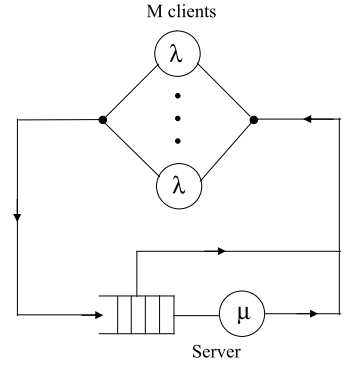
\includegraphics[scale=1]{figures/ex/cssystem.png}
\caption{Client-Server System}
\end{figure}

Client/Server con $M$ utenti. $\forall$ utente, in media dopo $\frac{1}{\lambda} s$ (EXP NEG) invia una richiesta al server. Il server esegue le richieste con FCFS. $\frac{1}{\mu} s$ è il tempo di servizio. Un utente genera una richiesta dopo che la precedente è stata servita. Ogni utente, indipendentemenete dagli altri, dopo un periodo di riflessione $(\frac{1}{\lambda})$, può quindi inviare le richieste al server. Gli utenti sono tuttavia impazienti e possono cancellare le richieste: a partire dall'invio delle richieste, dopo un tempo di durata media $\frac{1}{\gamma} s$, cancella la richiesta. Può cancellare solo se la richiesta NON sta venendo eseguita. Tempi di servizio, cancellazione e di riflessione sono rispettivamente i.i.d. e statisticamente indipendenti tra di loro; Quindi DTT, utilizzazione CPU, \dots

Modellazione di un sistema Web. Non è contemplata la possibilità che un utente si scocci e vada via. Condizioni di saturazione: Studio del sistema sotto-stress. $\max\{M\}$ per avere determinate prestazioni. Numero di utenti massimo che il server può sopportare, tollerare affinché si abbiano delle predeterminate prestazioni. $t\rightarrow \frac{1}{\lambda}$ per cliccare su un certo Hyperlink. 

Sistema reale Questo sistema reale descritto può essere modellato come una RETE DI CODE CHIUSA. Sistema a coda. Modello stocastico che rappresenta questo sistema reale descritto. Varie entità in gioco: \{\{utenti\}, server\}. Si parla di: \{tempi di riflessione, tempi di servizio, tempi di cancellazione\}. Server Web. Processo applicativo. Clienti + servitore + fila di attesa. Una rete di code è un insieme di code interconnesse tra di loro secondo una certa topologia. APERTA quando i clienti possono arrivare dall'esterno e partire verso l'esterno di questo sistema. CHUSA quando NON c'è la possibilità che arrivino dall'esterno o partano verso l'esterno. In tal caso il numero dei clienti è costante (Non si arriva e non si parte). Situazioni intermedie rendono il sistema non stabile. I blocchi di ritardo sono modellabili con delle code [$\mathord{\cdot}$/M/$\infty$]. Questa è una RETE DI CODE CHIUSA. $M=\cardinality{clienti}$. $M$ utenti nel sistema reale. Clienti + servitore. Un cliente si può trovare o nei blocchi di ritardo oppure nel sistema a coda. La presenza di un cliente nel blocco di ritardo rappresenta il fatto che nel sistema reale gli utenti possono avere un tempo di riflessione. Abbiamo $M$ unità di ritardo. Se un cliente è in un blocco di ritardo, il corrispondente utente nel sistema reale si trova in un periodo di riflessione. Il passaggio di un cliente dal blocco di ritardo verso il sistema a coda rappresenta il fatto che l'utente ha cliccato su un hyperlink: ha inviato una richiesta al server. Fila di attesa. Il passaggio di un cliente dalla fila di attesa verso il centro di servizio corrisponde al fatto che il server ha preso in considerazione la richiesta Web. Quando nel modello il cliente parte, andrà nuovamente nel blocco di ritardo. Il corrispondente utente nel sistema reale, avendo usufruito dell'erogazione del servizio, starà di nuovo pensando, scegliendo il successivo hyperlink da cliccare. C'è anche la possibilità che un cliente vada via dalla fila di attesa PRIMA ancora che venga servito. Ciò corrisponde alla situazione reale al fatto in cui un utente cancelli la propria richiesta in attesa, in coda. Possibilità che i clienti vadano via dalla fila di attesa. Anche quando un cliente va via dalla fila di attesa, giungerà nuovamente nei blocchi di ritardo. Modello stocastico che rappresenta bene il sistema reale.

Rete di code. Potrei risolverla con le tecniche adibite alla risoluzione di queste reti di code. Ma procederemo con i processi stocastici. Consideriamo il processo stocastico: $N(t)=\cardinality{clienti\ del\ sistema\ a\ tempo\ t}$ (Nel sistema a coda). Dinamica determinata dalle v.a.: \{tempi di riflessione, tempi di servizio, tempi di annullamento\}. Sono tutte v.a. exp-neg i.i.d. e statisticamente indipendenti tra di loro $\implies $ CMTC. DTT:

\begin{center}
\begin{tikzpicture}[->, >=stealth', auto, semithick, node distance=2.8cm]
\tikzstyle{every state}=[fill=white,draw=black,thick,text=black,scale=1]
\node[state]    (0)                     {$0$};
\node[state]    (1)[right of=0]   {$1$};
\node[state]    (2)[right of=1]   {$2$};
\node[state] (d) [right of=2] {\ldots};
\node[state]    (MM1)[right of=d]  {$M-1$};
\node[state]    (M)[right of=MM1]   {$M$};
\path
(0) edge[bend left]     node{$M\lambda$}         (1)
(1) edge[bend left]     node{$(M-1)\lambda$}         (2)
    edge[bend left,below]    node{$\mu$}            (0)
(2) edge[bend left]     node{$(M-2)\lambda$}           (d)
    edge[bend left,below]    node{$\mu+\gamma$}             (1)
(d) edge[bend left]         node{$(M-3)\lambda$}   (MM1)
	edge[bend left,below]   node{$\mu+2\gamma$}          (2)
(MM1)edge[bend left]    node{$(M-1)\lambda$}     (M)
     edge[bend left,below] node{$\mu+(M-2)\gamma$} (d)
(M) edge[bend left,below] node{$\mu+(M-1)\gamma$} (MM1);
\end{tikzpicture}
\end{center}

I clienti che NON si trovano nel sistema a coda saranno in una condizione di \underline{ARRIVO} nel sistema a coda. Il tempo che ci mette per uscire dal blocco di ritardo e giungere nel sistema a coda è $(\dots)\sim EXP-NEG(\lambda)$ i.i.d. indipendente dalle altre. Consideriamo uno stato non estremo. $0<i<M$. Supponiamo che al tempo $t$, $\underline{N(t)=i}=\cardinality{clienti\ in\ fila\ di\ attesa}+\cardinality{clienti\ nel\ centro\ di\ servizio}$. Avremo rispettivamente $i-1$ clienti in coda ed 1 nel centro di servizio. Se lo stato a tempo $t$ è i, avremo un certo numero $(M-i)$ in condizioni di arrivo. Se lo stato è i, la successiva transizione di stato potrà essere determinata da: un arrivo nel sistema a coda, quando finisce un servizio in corso, oppure a causa di un annullamento di una delle $(i-1)$ richieste pendenti. In questo caso, si avrà una transizione di stato (variazione di stato). $t \rightarrow$ successivo arrivo. Indichiamo al solito con $\xi_{R(t)}|_i\sim EXP ((M-i)\lambda) = \min\{(\dots)\}$, ovvero pari al minimo delle v.a. che rappresentano il tempo di arrivo residuo del k-esimo cliente nel blocco di ritardo (NO TEMPO DI INTERARRIVO!). Tempo che passa invece dall'istante $t$ al successivo completamento dell'erogazione del servizio è $\eta_{R(t)}|_i\sim EXP(\mu)$. Il tempo che passa dall'istante presente $t$ ed il successivo annullamento della richiesta è una v.a. definita in tal modo: $\theta_{R(t)}|_i\sim EXP[(i-1)\gamma]=\min\{(\dots)\}$, ovvero pari al minimo delle v.a. che rappresentano il tempo di annullamento residuo al tempo $t$. Ricordiamo: $\phi_i(t)\sim EXP(-q_{ii})$, ovvero il tempo di soggiorno nello stato $i$. Inoltre, $\Pr\{\phi_i(t)>\tau\}$, la sua CDF complementare, è pari alla probabilità che in $\tau$ NON ci sia nessun arrivo, NON ci sia la fine del servizio in corso e NON vi sia annullamento di una richiesta; il tutto condizionato con il fatto di trovarci nello stato $i$. Per indipendenza, essa è pari al prodotto delle rispettive probabilità, ovvero:

\[
	\Pr\{\phi_i(t)>\tau\} = [\Pr\{\xi_{R(t)} > \tau\ |\ i\}\Pr\{\eta_{R(t)} > \tau\ |\ i\}\Pr\{\theta_{R(t)} > \tau\ |\ i\}] =
\]
\[	
	= \e^{-(M-i)\lambda\tau}\e^{-\mu\tau}\e^{-(i-1)\gamma\tau} = e^{[\underline{-[(M-i)\lambda+\mu+(i-1)\gamma] = x]\tau}}
\]

Cosicché $(-q_{ii}=[x]) > 0$, ovvero abbiamo trovato la VELOCIT\`A TOTALE DI USCITA. Procediamo al solito modo:

\[
	\underline{\tau_{i,i+1}} = \frac{q_{i,i+1}}{-q_{ii}} = (\dots)
\]

dove $[-q_{ii}=[(M-i)\lambda+\mu+(i-1)\gamma]]$; il termine sottolineato è invece la probabilità che, lasciando lo stato $i$, migriamo verso lo stato $i+1$.

\[
	(\dots) = \Pr\{\xi_{R(t)} < \underline{\min\{\eta_{R(t)},\ \theta_{R(t)}\}}\} = (\dots)
\]

ove tale quantità rappresenta la probabilità che il successivo arrivo preceda il verificarsi dei due altri eventi. Tramite il teorema delle probabilità totali, otterremo alla fine:

\[
	(\dots) = \frac{(M-i)\lambda}{(M-i)\lambda+\mu+(i-1)\gamma} \implies
\]
\[
	\left\{
	\begin{aligned}
	&[q_{i,i+1} = (M-i)\lambda]\\
	&[q_{i,i-1} = \mu+(i-1)\gamma]
	\end{aligned}
	\right.
\]

Abbiamo quindi capito perché i tassi di transizione sono proprio questi. 

\[
	N(t)=0 \implies \underline{\phi_0(t)}\sim EXP(-q_{00}) =\underline{\xi_{R(t)}|_0} \sim EXP(M\lambda)
\]

$\implies \underline{-q_{00} = M\lambda}$. Se invece consideriamo lo stato $N(t)=M$ (tutti i clienti nel sistema a coda), avremo 0 clienti invece nel blocco di ritardo. La successiva transizione di stato sarà determinata o dall'annullamento di una richiesta o dalla fine dell'erogazione del servizio in corso:

\[
	\phi_M(t) = \min\{\eta_{R(t)}, \theta_{R(t)}\} \sim EXP((M-1)\gamma+\mu)
\]

$\implies -q_{MM} = (M-1)\gamma+\mu$. Quindi in realtà possiamo considerare valida la definizione di $-q_{ii}$ per $1<i\leq M$, in realtà.

CATENA \underline{\underline{ERGODICA}} $\iff$ OMOGENEA, IRRIDUCIBILE e $\cardinality{stati}<+\infty\iff$ numero di stati finito. Nel sistema a coda più di $M$ clienti NON ci possono essere $(\iff \cardinality{stati}<+\infty)$. 

CMTC tempo continuo, nascita e morte $\implies$

\[
	\left\{
	\begin{aligned}
	&[\pi_i=\pi_0 \lambda^i \frac{M!}{(M-i)!} \frac{1}{\prod_{k=0}^{i-1}{(\mu+k\gamma)}}]\\
	&\pi_0 = \frac{1}{1+\sum_{i=1}^M{\lambda^i \frac{M!}{(M-i)!} \frac{1}{\prod_{k=0}^{i-1}{(\mu+k\gamma)}}}}
	\end{aligned}
	\right.
\]

ove $\pi_0$ lo otteniamo con la condizione di NORMALIZZAZIONE. $i-1$ richieste pendenti ed un'altra in esecuzione nella CPU (del Server). $\rho$ è l'UTILIZZAZIONE, ovvero la frazione di tempo in media nella quale il servitore è impegnato a servire i clienti: $[\rho=1-\pi_0]$. Adesso dobbiamo valutare il throughput medio (throughput della CPU). Numero medio di richieste servite dalla CPU $\forall$ unità di tempo. Quando la CPU termina il servizio della richiesta, il cliente partirà dal centro di servizio. Applichiamo \underline{Little} ed otteniamo:

\[
	[\rho=\frac{\lambda_S}{\mu} \implies \lambda_S = \mu\rho = \mu(1-\pi_0)]
\]

Se consideriamo il prodotto $\pi_i[\mu+(i-1)\gamma]$, otteniamo la frequenza delle transizioni di questo tipo. Numero medio di volte che accade questa transizione $\forall$ unità di tempo. Consideriamo allora: $\underline{\pi_i\mu} + \underline{\pi_i(i-1)\gamma}$. Il primo termine sottolineato è la frequenza delle transizioni che portano da $i$ ad $i-1$ A CAUSA della fine di un servizio, mentre il secondo termine sottolineato rappresenta la frequenza delle transizioni $i\rightarrow i-1$ A CAUSA dell'annullamento di una richiesta. 

\[
	\left\{
	\begin{aligned}
	&[\lambda_S = \mu\pi_1 + \mu\pi_2 + \mu\pi_3 + \dots + \mu\pi_M = \mu(1-\pi_0) = \mu\rho]\\
	&[\lambda_R = \gamma\pi_2 + 2\gamma\pi_3 + 3\gamma\pi_4 + \dots + (M-1)\gamma\pi_M]
	\end{aligned}
	\right.
\]

Ove la seconda equazione rappresenta la velocità di partenza dei clienti dalla fila di attesa. Per trovare il numero medio di clienti in stato di riflessione, quindi, applichiamo nuovamente Little:

\[
	\bar{N}_R = \underline{(\lambda_S+\lambda_R)} \frac{1}{\lambda}
\]
\[
	\bar{N}_R = 0 \pi_M + 1\pi_{M-1} + 2\pi_{M-2} + \dots + M\pi_0
\]

Non è infatti difficile riconoscere ivi una media. Si può dimostrare che i due termini sono praticamente uguali e consistenti utilizzando le equazioni di BILANCIAMENTO LOCALE:

\[
	\pi_{i-1}(M-i+1)\lambda = \pi_i[(\mu+(i-1)\gamma)]
\]

Assumendo che le richieste NON possano essere cancellate, abbiamo che:

\[
	\underline{\E[R]} + \frac{1}{\lambda}
\]

Il primo termine sottolineato è il tempo medio di risposta, ove con $R$ intendiamo il tempo di risposta del sistema a coda, mentre il secondo addendo è al solito il tempo medio di riflessione. Un utente invierà una richiesta ogni $(\E[R]+\frac{1}{\lambda})$. Abbiamo $M$ richieste. $M$ utenti invieranno $M$ richieste alla seguente velocità:

\[
	(\frac{M}{\E[R]+\frac{1}{\lambda}}) = \underline{\lambda_S} = \mu\rho
\]

Dato che un utente NON può inviare una richiesta PRIMA che la precedente sia soddisfatta. Ove adesso il termine sottolineato rappresenta la velocità di arrivo delle richieste. Cosicché abbiamo:

\[
	\frac{M}{\mu\rho} = \E[R]+\frac{1}{\lambda} \implies \E[R] = \frac{M}{\mu\rho} -\frac{1}{\lambda} \implies \E[R]=\mathord{\cdot}{(M)}
\]

Se abbiamo 1 solo cliente $\iff M\rightarrow 1 \implies \E[R]=\frac{1}{\mu}$ NO fila di attesa. $M\uparrow (\mathord{\cdot}\to\infty) \implies \rho\to1 \implies \E[R]=(\frac{M}{\mu}-\frac{1}{\lambda})$, la quale quantità corrisponderebbe all'ASINTOTO OBLIQUO del grafico di $\E[R]$ in funzione di $M$.

L'asintoto viene in letteratura chiamato \textit{HEAVY LOAD asymptote}, mentre la retta ovviamente corrisponderebbe al \textit{LIGHT LOAD asymptote}. Il valore di $M$, $M^\star$ per il quale i due asintoti si incontrano, viene chiamato in letteratura \textit{SATURATION NUMBER}, ovvero il valore di $M=M^\star$ per il quale il sistema si considera in SATURAZIONE. Carico che può essere tollerato da un servizio, da un server:

\[
	\frac{1}{\mu} = \frac{M}{\mu} -\frac{1}{\lambda} \implies \frac{M}{\lambda} = \frac{1}{\mu}+\frac{1}{\lambda} \implies M^\star = (1+\frac{\mu}{\lambda})
\]

Tale valore rappresenta quindi il valore di $M$ per il quale il sistema è in saturazione. Se $\frac{1}{\lambda}=15 s$, e nel caso in cui $\frac{1}{\mu}=1 s$, abbiamo $\implies M^\star = 16 = 1+(15=\frac{\mu}{\lambda})$.

Ricordiamo che:

\[
	\underline{R(t) = \Pr\{X > t\}}
\]

è l'AFFIDABILIT\`A.

\subsection{RECAP}

M/M/1. Stato: $N(t) := \cardinality{clienti\ nel\ sistema\ a\ coda}$ (nell'intero sistema a coda). $N_q(t) := \cardinality{clienti\ in\ fila\ di\ attesa}$. CATENA DI MARKOV (OMOGENEA). Noto lo stato presente è possibile determinare l'evoluzione futura del processo in termini probabilistici, senza conoscere la storia passata (lo stato presente riassume tutta l'evoluzione passata). CATENE = stato discreto. Dell'evoluzione futura fa parte anche il tempo di soggiorno residuo $\phi_i(t) \sim EXP(-q_{ii})$. Se noto lo stato del processo nell'istante presente non riesco a determinare la distribuzione del tempo di soggiorno residuo, nel tempo in cui mi trovo, possiamo dire che NON riusciamo a determinare l'evoluzione futura. Evoluzione futura in termini probabilistici.

M/M/1. $\cardinality{clienti\ in\ fila\ di\ attesa}=\underline{N_q(t) = 0}$. Supponiamo vi siano 0 clienti (informazione che ho sullo stato presente del processo). Proviamo a determinare la distribuzione del tempo di soggiorno residuo in questo istante, MA non so se ci sono clienti nel centro di servizio. 

Supponiamo che vi sia un cliente nel centro di servizio (servitore occupato). Se termina quel servizio, si avrà una transizione di stato? NO. $\underline{\phi_0}(t)$ (0 clienti in fila di attesa). Se c'è 1 cliente, $\phi_0(t)\sim EXP(\lambda)$. Tempo di interarrivo residuo. Ma se non c'è nessuno, quella v.a. non sarà mica pari al tempo di interarrivo residuo. La transizione di stato si ha se arriva un cliente e ne arriva un altro. (Quindi se mettiamo insieme l'informazione invece riusciamo). Ma se includiamo quell'informazione torniamo alla precedente definizione di stato.

\section{RETI DI CODE}

Una rete dati di tipo switched può essere modellata mediante una rete di code. Queste code interagiscono tra di loro. Uno stream di pacchetti in partenza da una coda potrà andare a visitare un'altra coda dopo un merging con pacchetti provenienti da un'altra coda. [MERGING = POOLING]. Quindi una volta acceduti alla rete (superata la coda di accesso), si crea (si viene a creare) una correlazione tra i tempi di interarrivo dei pacchetti e quelli di trasmissione. Quindi viene meno l'ipotesi iniziale di indipendenza tra tempi di servizio e tempi di interarrivo. Adesso i tempi di servizio corrispondono ai tempi di trasmissione. Immaginiamo che i pacchetti arrivino alla rete con un processo di $\lambda$-POISSON. Nodo di accesso. Supponiamo che le lunghezze dei pacchetti siano v.a. equidistribuite statisticamente (i.d.), mutuamente indipendenti (con un certo valor medio), ed indipendenti dai tempi di interarrivo dei pacchetti al nodo di accesso. Tempi di trasmissione $\sim EXP(\mathord{\cdot})$. Data una certa capacità, le lunghezza dei pacchetti sono collegate ai tempi di trasmissione. Supponiamo che tempi di elaborazione e propagazione siano trascurabili. FCFS disciplina di coda. Serve però un'ipotesi aggiuntiva riguardo la dimensione dei buffer $(d=+\infty)$, ovvero illimitata.

Sistema reale: insieme dei due router con linee random (coda in serie). Il primo sistema è un M/M/1, per le ipotesi fatte. Si osservi il ramo che collega il primo centro di servizio con l'ingresso nel secondo buffer, e si effettuino delle analisi sulla eventuale dipendenza tra tempi di servizio e tempi di interarrivo. \`E evidente che le due grandezze sono in \textit{CORRELAZIONE}. Non posso quindi parlare di coda M/M/1 per il secondo sottosistema. A parte che non sappiamo che processo degli arrivi sia. Lo sapremo mediante teorema di \underline{BURKE}.

\begin{center}
\begin{figure}[H]
\centering
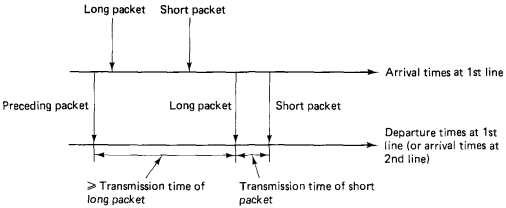
\includegraphics[scale=1]{figures/klnrk.png}
\caption{Timing Diagram of packet arrivals and departures completions in a system of two transmission lines in tandem} 
\end{figure}
\end{center}

Supponiamo che ad un certo istante termini la trasmissione di un pacchetto precedente. Poi, arrivi un pacchetto grande alla prima coda, il quale, trovandola vuota e notando disponibile il centro di servizio, ivi vi entra subito e viene iniziato il servizio (trasmissione). Finita la trasmissione di questo pacchetto, possiamo osservare che il tempo di interarrivo alla seconda coda (distanza temporale tra l'istante di arrivo del precedente pacchetto e l'istante di arrivo di questo), è risultato maggiore del tempo di trasmissione del pacchetto grande. Questo sarebbe già sufficiente per compromettere l'indipendenza. Si noti comunque che, se durante la trasmissione arriva un piccolo pacchetto alla prima coda, trovando il centro di servizio occupato, è costretto ad attendere in fila di attesa. Quando finirà la trasmissione del pacchetto grande, il piccolo potrà essere trasmesso. Ma a questo punto osserveremo un tempo di interarrivo (tra il grande ed il piccolo pacchetto) alla seconda coda praticamente uguale al tempo di trasmissione del piccolo pacchetto. Notiamo che vale: $\underline{t_{IA}\geq t_T}$, ovvero il tempo di interarrivo al secondo router è maggiore uguale del tempo di trasmissione nel primo router (in particolare sarà più grande se e solo se il secondo pacchetto trova la prima coda vuota (incluso il centro di servizio) al suo arrivo). Dal momento che nelle reti dati tipicamente avremo una lunghezza costante dei pacchetti, saranno quindi correlati anche i tempi di interarrivo al secondo sottosistema con i suoi tempi di servizio, dal momento che le lunghezze dei pacchetti influenzano i tempi di trasmissione, e quindi di servizio, anche se capacità dei link è differente tra i due. $\implies$ NO INDIPENDENZA. Leonard Kleinrock, il pioniere nella Ricerca delle Reti delle Code, ha risolto brillantemente questo problema. Andare a combinare (MERGING) su una certa coda flussi di pacchetti provenienti da altre code ha l'effetto di ripristinare l'indipendenza tra tempi di interarrivo a tempi di trasmissione. Se nel nostro esempio osserviamo al secondo router pacchetti di un altro router (nodo), non c'è più correlazione! Ripristino dell'ipotesi di INDIPENDENZA. La possibilità che accada questo evento dipende dal livello di comunicazione e di traffico! Più la rete è magliata (più merging di differenti flussi), e più è intenso il traffico, più è probabile che accadano eventi di questo tipo. La rete deve essere \textit{DENSAMENTE CONNESSA} ed il traffico deve essere intenso. Cosicché per una rete densamente connessa e per intensità di traffico medio-alta, possiamo ritenere valida la cosiddetta \textit{\textbf{APPROSSIMAZIONE DI INDIPENDENZA DI KLEINROCK}}. Intensità di traffico medio-alta inoltre! Possiamo mantenere sempre valida l'indipendenza tra tempi di interarrivo e tempi di trasmissione (servizio).

\subsection{RETE DI CODE APERTA}

Rete di code: insieme di code interconnesse tra di loro. Supponiamo di avere il seguente scenario:



Stiamo rappresentando con una rete di code un sistema di Elaborazione.

Clienti/Servitori/Fila di Attesa. Questa è la topologia della rete di code. Stiamo modellando un sistema di elaborazione. I clienti corrispondono alle richieste di esecuzione dei job (la presenza di un clientre in $\mu_1$ significa che si sta eseguendo quel job). I job stanno arrivando dall'esterno. Nodi alias stazioni di servizio. Il nodo 0 corrisponde al mondo esterno, dal quale possono arrivare i clienti. SINGLE CLASS \underline{OPEN}. Una rete si dice \underline{aperta} quando i clienti possono arrivare dall'esterno e fluire (partire) verso l'esterno. Per una CHIUSA (\underline{CLOSED}) è il contrario di quella aperta. Per una CHIUSA il numero di clienti è costantè (\textit{ISARITHMIC CONGESTION CONTROL}). $\exists M$ percorsi nella rete. Una rete di code, quando in essa i clienti arrivano esattamente se partono gli altri: 1 entra $\leftrightarrow$ 1 esce, può essere considerata chiusa. A volte possiamo volutamente limitare ad $M$ il numero di pacchetti che transitano. 

\underline{SINGLE CLASS OPEN}. Tornando al nostro caso, i clienti arrivando dall'esterno nel nostro sistema a coda, possono visitare solo il nodo 1 $\iff \underline{\underline{p_{01}=1}}$. Ma potrebbero $\exists(p_{0i}\neq 1)$. Leggi delle probabilità:

\[
	[p_{11}+p_{10}+p_{12}+p_{13}+p_{14} = 1]
\]

Similmente per gli altri nodi. Una volta visitato il nodo 2, il cliente potrà visitare soltanto il nodo 1. Questo vale anche per gli altri nodi 3-4! ($\iff [p_{21}=p_{31}=p_{41}=1]$. SINGLE CLASS = \{singola classe di clienti\}. Ma potrebbero esserci più classi di clienti. Per una rete di code con vari nodi definiamo:

\[
	[\underline{p_{ij} := ROUTING\ PROBABILITY}]
\]

o \underline{PROBABILIT\`A DI ROUTING}. (collegate ai protocolli di instradamento). Si potrebbero definire delle probabilità per differenti classi. Per altri stream potrei scegliere delle differenti destinazioni. Si modellino i vari stream nella rete ($\exists K$ classi ad esempio) come delle "classi di clienti". Sia: $N=\cardinality{nodi}$. Indichiamo con $K$ il vettore riga: $\underline{K} := (K_1,K_2,\ \dots,\ K_N)$, ove tale vettore rappresenta il numero di clienti NEI VARI NODI. Difatti, $K_i:=\cardinality{clienti\ al\ nodo\ "i"}$. E quindi: $K=\sum_{i=1}^N{K_i} := \cardinality{clienti\ nella\ rete}$. Definiamo: $[m_i\geq 1]:=\cardinality{servitori\ paralleli\ al\ nodo\ "i"}$. Indichiamo con $\mu_i$ la velocità del singolo servitore al nodo "i" (In generale possiamo avere velocità differenti per il nodo "i"). Noi considereremo servitori alla stessa velocità. Introduciamo il concetto di [Soluzione in forma PRODOTTO].

$p_{ij}$ = probabilità di routing $\implies p_{0,j}$ = probabilità che un cliente in arrivo dall'esterno vada a visitare il nodo $j$. Similmente, $p_{i,0}$ = probabilità che un cliente in partenza dal nodo $i$, lasci la rete. Cosicché: $pi_{i,0} = 1-\sum_{j=1}^N{p_{ij}}$. $\lambda_{0i}$ = velocità di arrivo dei clienti dall'esterno al nodo "i". Indichiamo con $\lambda$ la velocità totale di arrivo dei clienti dall'esterno $\iff \lambda=\sum_{i=1}^N{\lambda_{0i}}$. La velocità totale sarà tale che: $\lambda_{0i}=\lambda p_{0i}$. Indicando con $\lambda_i$ la velocità TOTALE di arrivo dei clienti al nodo $i$ e con $\lambda_j$ la velocità di partenza delle altre code, otteniamo:

\[
	[\lambda_i=\lambda_{0i}+\sum_{j=1}^N{\lambda_jp_{ji}}]
\]

con $i=1,2,\ \dots,\ N$. Dividendo membro a membro per $\lambda$ otteniamo:

\[	
	\frac{\lambda_i}{\lambda} = \frac{\lambda_{0i}}{\lambda} + \sum_{j=1}^N{\frac{\lambda_j}{\lambda}p_{ji}}
\]

con $i=1,2,\ \dots,\ N$. Queste sono le cosiddette \underline{EQUAZIONI DEL TRAFFICO}. Definiamo allora:

\begin{defn}{\textbf{Visit Ratio}}

Definiamo il VISIT Ratio come:

\[
	[e_i := \frac{\lambda_i}{\lambda}]
\]
\end{defn}

Esso rappresenta il numero medio di visite al nodo "i" $\forall$ arrivo dall'esterno. Quante volte un cliente IN ARRIVO DALL'ESTERNO visita il nodo "i" prima di lasciare la rete. Ad esempio:

\[	
	\lambda_i=20\ clienti/s,\ \lambda=2\ clienti/s,\ \frac{\lambda_i}{\lambda}=(10/2 = 5)\ clienti/s
\]

Diamo ora un'altra definizione:

\begin{defn}{\textbf{Service Demand}}

Definiamo $D_i$ service demand la quantità totale di servizio che in media un cliente richiede in un certo nodo:

\[
	\left\{
	\begin{aligned}
	&[e_i = p_{0i} + \sum_{j=1}^N{e_jp_{ji}}]\\
	&[D_i := e_i(\frac{1}{\mu_i})]
	\end{aligned}
	\right.
\]

\end{defn}

Si noti che $D_i$ è una quantità temporale!


Consideriamo la seguente rete di code: Due code a singolo router in serie e supponiamo che il processo degli arrivi al nodo "1" sia di $\lambda$-POISSON, che i tempi di servizio dei clienti alla prima ed alla seconda coda siano v.a. $(\dots)\sim EXP(\mu_1)$ per la prima e $(\dots)\sim EXP(\mu_2)$ per la seconda, mutuamente indipendenti ed \underline{indipendenti} dal processo degli arrivi alle code (tempi di interarrivo dei clienti alle code). QUESTE NON SONO RETI DATI! Ma generiche reti di code. Supponiamo $(d=+\infty)$ e disciplina di coda FCFS. Con le ipotesi viste la prima coda è M/M/1. Riguardo alla seconda coda, il processo degli arrivi dei clienti alla seconda coda corrisponde al tempo di partenza (al processo delle partenze dei clienti del nodo 1). Quindi è una $\mathord{\cdot}$/M/1 (Il processo degli arrivi NON può essere considerato, descritto indipendentemente dal resto della rete). Processo delle partenze. Questo fatto ci fa comprendere l'importanza di caratterizzare i processi delle partenze dei clienti delle code. Teorema di BURKE che fa la caso nostro:

\begin{thrm}{\textbf{Teorema di BURKE}}

Si consideri un sistema a coda M/M/1 $\lor$ M/M/m $\lor$ M/M/$(m=\infty)$. Sia $\lambda$ la velocità di arrivo dei clienti (processi degli arrivi dei clienti). Supponiamo di stare in condizioni di regime:

\begin{itemize}

\item{a)} Il processo delle partenze è \underline{di POISSON}, a velocità $\lambda$;
\item{b)} $\forall$ istante $t$, $\cardinality{clienti\ nel\ sistema}$ NON dipende dalla sequenza delle partenze fino a $t$. Esso dipende SICURAMENTE dagli arrivi che ci sono stati fino a $t$, SICURAMENTE dai tempi di servizio dei clienti che SONO stati effettivamente serviti;
\end{itemize}
\end{thrm}

Per dimostrarlo si dovrebbero utilizzare le CATENE DI MARKOV \textit{REVERSIBILI} (Ragionare andando nel verso opposto come tempo $\iff$ guardando l'evoluzione a ritroso).
Determinare la cosiddetta \textit{OCCUPANCY DISTRIBUTION}, ove intendiamo la probabilità che vi siano $K_1$ clienti nella "coda 1" e $K_2$ clienti nella "coda 2" a regime (probabilità congiunta):

\[
	\Pr\{K_1\ clienti\ nella\ "coda\ 1",\ K_2\ clienti\ nella\ "coda\ 2"\} =
\]
\[
	= \Pr\{K_1,K_2\} := \underline{\pi(K_1,K_2)}
\]

Notazione con pedici anche possibile. Distribuzione congiunta dei clienti nelle VARIE CODE. Una rete di code si dice STABILE se $\forall$ sistema a coda di cui si compone è STABILE. CONDIZIONE DI STABILIT\`A:

\[	
	[(\rho<1) \iff (\frac{\lambda}{\mu} < 1) \iff \lambda<\mu] \implies
\]
\[
	\implies
	\left\{
	\begin{aligned}
	&\rho_1=\frac{\lambda}{\mu_1} < 1 \iff \lambda<\mu_1\\
	&\rho_2=\frac{\lambda}{\mu_2} < 1 \iff \lambda<\mu_2
	\end{aligned}
	\right.
\]

Imposta la stabilità delle code e delle reti di code, utilizzo il teorema di BURKE. Sfruttiamo la parte a) del teorema. Processi degli arrivi in 2 di POISSON. Se guardiamo "2", isolatamente sarebbe un M/M/1 adesso (grazie a BURKE). Sfruttiamo adesso la parte b) di BURKE. Consideriamo le v.a. casuali che rappresentano il numero di clienti in "1" ed in "2":

\[
	\Pr\left\{
	\begin{aligned}
	&N_1(t) = K_1\\
	&N_2(t) = K_2
	\end{aligned}
	\right.
\]

Abbiamo $\{N_1(t),N_2(t)\},\ \forall t$. Risulta:

\[
	N_1(t) \neq \mathord{\cdot} N_2(t)
\]

grazie a Burke $\implies N_1(t),N_2(t)$ sono v.a. indipendenti $\implies$

\[
	\pi_{K_1,K_2} := \pi(K_1,K_2) = \pi(K_1)\pi(K_2)
\]

pari ovvero al prodotto delle due distribuzione marginali dei sistemi a coda visti in isolamento. Soluzione in FORMA PRODOTTO della OCCUPANCY DISTRIBUTION. In realtà i singoli sistema a coda NON stanno in isolamento! \`E una rete di code infatti. Riprendendo l'esempio delle M/M/1, abbiamo:

\[
	\{\lambda,\mu\} \implies \underline{\pi(K_1,K_2)} = [(1-\rho_1)\rho_1^{K_1}][(1-\rho_2)\rho_2^{K_2}]
\]

dove abbiamo: $\{(\rho_1=\frac{\lambda}{\mu_1}),\ (\rho_2=\frac{\lambda}{\mu_2})\}$. Ove abbiamo semplicemente utilizzato le espressioni trovate per la M/M/1. Allo stesso risultato si poteva arrivare senza sfruttare Burke ed analizzando con approccio Markoviano le seguenti reti di code, utilizzando una definizione di stato bidimensionale (multi-indice) (al tempo $t$). Sfruttiamo l'EQ. DI BILANCIAMENTO TOTALE dei flussi per una CATENA ERGODICA. Dovremo però aggiungere ovviamente la condizione di normalizzazione. Si arriva a scrivere:

\[
	\pi_{K_1,K_2} = (1-\frac{\lambda}{\mu_1})(1-\frac{\lambda}{\mu_2})(\frac{\lambda}{\mu_1})^{K_1}(\frac{\lambda}{\mu_2})^{K_2} =
\]
\[	
	= [\underline{((1-\frac{\lambda}{\mu_1})(\frac{\lambda}{\mu_1})^{K_1} = \pi_1(K_1))}][\underline{((1-\frac{\lambda}{\mu_2})(\frac{\lambda}{\mu_2})^{K_2} = \pi_2(K_2))}] = \underline{\pi(K_1)\pi(K_2)}
\]

Proviamo a sostituirle nelle equazioni di bilanciamento.

Giustificazione matematica. $\underline{(K_1,K_2)}$. Quindi ai fini della \underline{Occupancy Distribution}, la distribuzione congiunta è pari al prodotto delle distribuzioni marginali.

\subsection{Feed-Forward (Reti di code ACICLICHE)}

Tutte le reti di code che comprendono code del tipo: \{$\mathord{\cdot}$/M/1, $\mathord{\cdot}$/M/m, $\mathord{\cdot}$/M/$\infty$\} le quali ricevono arrivi sia da altre code della rete, sia dall'esterno, secondo processi di POISSON, e che non permettono a nessun cliente di ritornare ad una coda già visitata (SENZA CICLI), sono risolubili in forma prodotto. ACICLICHE $\iff \nexists$ CICLI. Per come sono fatte queste reti di code i processi degli arrivi sono di POISSON alle varie CODE.

\subsubsection{SEARCH ENGINE - MOTORI DI RICERCA}

Si consideri una porzione di rete in cui sono presenti tre motori di ricerca organizzati gerarchicamente in due livelli (vedi figura): a livello più alto e’ presente il motore MC, mentre a livello gerarchico più basso sono presenti i motori MA e MB. Gli utenti sono connessi al livello gerarchico più basso. Una richiesta di ricerca viene presentata da un generico utente al proprio motore. Questo, se dopo averla elaborata, non e’ in grado di soddisfarla, la reindirizza verso il motore MC che e’ sicuramente in grado di risolverla. Si assuma che:

\begin{itemize}

\item{i)} le richieste di ricerca da parte degli utenti del gruppo A siano presentate in accordo ad un processo di Poisson con parametro $\lambda_A\ req/min$;
\item{ii)} le richieste di ricerca da parte degli utenti del gruppo B siano presentate in accordo ad un processo di Poisson con parametro $\lambda_B\ req/min$;
\item{iii)} in ogni motore un unico processore elabori le richieste in modalità FCFS e con tempi che sono v.c. indipendenti distribuite secondo una ddp esponenziale negativa a valor medio pari, rispettivamente per i tre motori $M_A$, $M_B$, e $M_C$, a $T_A$ sec, $T_B$ sec e $T_C$ sec;
\item{iv)} una richiesta sia soddisfatta con probabilità $\alpha$ da un motore di livello basso;
\item{v)} sia trascurabile il tempo necessario ad inoltrare una richiesta al motore $M_C$.  

\end{itemize}

Calcolare:

\begin{itemize}

\item{a)} il fattore di utilizzazione del processore nel motore $M_C$;
\item{b)} il tempo medio di risoluzione di una richiesta;
\item{c)} il tempo medio di risoluzione di una richiesta da parte degli utenti del gruppo A. 
  
\end{itemize}

\begin{center}
\begin{figure}[H]
\centering
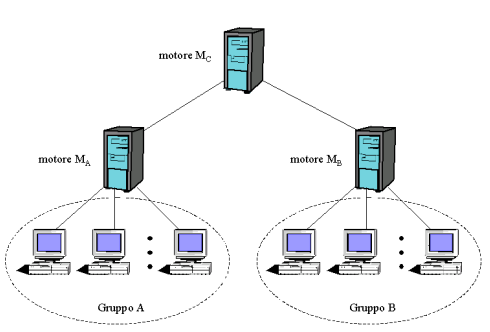
\includegraphics[scale=1]{figures/ex/se.png}
\caption{Hierarchical Search Engines}
\end{figure}
\end{center}

Risoluzione:

Tre motori di ricerca organizzati gerarchicamente in tre livelli. Gli utenti sono connessi al livello gerarchico più basso. $\{\lambda_A,\lambda_B\}\ req/min$, processi di POISSON. Richieste in modalità FCFS. Per quanto concerne i tempi di servizio, siamo dinanzi delle ddp esponenziali con i seguenti tempi di servizio medi, rispettivamente: $\{T_A, T_B, T_C\}s$. $M_C=?$ (fattore di utilizzazione). C'è da aggiungere un'ipotesi sulle dimensioni delle file di attesa: File di attesa illimitate $\iff (d=+\infty)$. Se qualcuna fosse un collo di bottiglia ci sarebbe scritta la dimensione $(\iff d<+\infty)$. Reti di code ACICLICHE. Processo degli arrivi dall'esterno di POISSON. Processo degli arrivi alle varie code di POISSON. Applicabile/applicato il teorema di BURKE. Abbiamo: $\{\mu_A=\frac{1}{T_A},\ \mu_B=\frac{1}{T_B},\ \mu_C=\frac{1}{T_C}\}$. Parametri della ddp esponenziale negativa. Popolazione illimitata $\iff (e=+\infty)$. Processo degli arrivi di POISSON. Rete ACICLICA $\iff$ feedforward network. Mi trovo dinanzi una rete di code. I processi degli arrivi sono di POISSON. Le reti A e B sono delle M/M/1. Viste in isolamento sono delle M/M/1. $\{K_A,\ K_B,\ K_C\}$ ci servono per definire la Occupancy Distribution (Burke + Splitting/Pooling). Code M/M/1 viste in isolamento $\iff$ grazie alla Soluzione in forma prodotto. Dobbiamo applicare le EQUAZIONI DEL TRAFFICO. La velocità di arrivo al sistema $M_C$ sarà:

\[
	\lambda_A(1-\alpha) + \lambda_B(1-\alpha) = (1-\alpha)(\lambda_A+\lambda_B) := \lambda_C
\]

I clienti NON si perdono! Se $\lambda_A$ arrivano nel primo sistema, $\lambda_A$ ne partiranno! Lo stesso dicasi per $M_C$. Per la STABILIT\`Adella rete di code dobbiamo imporre che $\forall$ sistema vi sia STABILIT\`A. Stabilità di ogni singolo sistema a coda:

\[
	\left\{
	\begin{aligned}
	&\rho_A = \frac{\lambda_A}{\mu_A}<1 \iff \lambda_A<\mu_A\\
	&\rho_B = \frac{\lambda_B}{\mu_B}<1 \iff \lambda_B<\mu_B\\
	&\rho_C = \frac{\lambda_C}{\mu_C}<1 \iff \lambda_C<\mu_C
	\end{aligned}
	\right.
\]

Analogamente... tre motodi di ricerca. Livello didattico. Nel calcolare $\lambda_C$ abbiamo anche risolto la prima domanda: $\rho_C=\frac{\lambda_C}{\mu_C}$, ovvero il FATTORE DI UTILIZZAZIONE del servitore nel nodo $M_C$. 

Tempo medio di risoluzione di una richiesta. L'arrivo nella rete di code di una richiesta corrisponde all'invio di una richiesta da parte di un utente. Tempo medio di risoluzione di una richiesta = tempo medio di permanenza nell'intero sistema. Clienti dall'esterno + Clienti in partenza $\leftarrow$ risoluzione di una richiesta. Si applichi Little:

\[
	[\bar{N}_{TOT} = \lambda_{TOT}\bar{R}] \implies \bar{R} = \frac{\bar{N}_{TOT}}{\lambda_{TOT}}
\]

$\bar{R}$ è quello che mi interessa. Sappiamo che: $\underline{\lambda_{TOT} = \lambda_A+\lambda_B}$, ovvero la velocità totale di arrivo dei clienti dall'esterno. Per un M/M/1 $\mathord{\cdot}(\lambda,\mu)$ il numero medio di clienti è: $(\bar{N}=\frac{\lambda}{\mu-\lambda})$. Lo dobbiamo però applicare ai vari sottosistemi. Somma dei numeri medi di clienti (a regime ovviamente):

\[
	[N_{TOT}=\bar{N}_A+\bar{N}_B+\bar{N}_C]\\
\]

sapendo che:

\[
	\left\{
	\begin{aligned}
	&\bar{N}_A = \frac{\lambda_A}{\mu_A-\lambda_A}\\
	&\bar{N}_B = \frac{\lambda_B}{\mu_B-\lambda_B}\\
	&\bar{N}_C = \frac{\lambda_C}{\mu_C-\lambda_C}
	\end{aligned}
	\right.
\]

Quindi abbiamo:

\[
	\bar{R} = \frac{N_{TOT}}{(\lambda_A+\lambda_B=\lambda_{TOT})}
\]

Per sapere invece il tempo medio di risoluzione di una richiesta da parte degli utenti del gruppo A $\iff R_A=?$, sapendo che per un M/M/1 vale:

\[
	\left\{
	\begin{aligned}
	&\bar{N}=\frac{\lambda}{\mu-\lambda}\\
	&\bar{T}=\frac{1}{\mu-\lambda}
	\end{aligned}
	\right.
\]

Allora si riconosce subito la media di una v.a.:

\[
	\bar{R}_A = \alpha[\frac{1}{\mu_A\lambda_A}] + (1-\alpha)[\frac{1}{\mu_A\lambda_A} + \frac{1}{\mu_C-\lambda_C}] =
\]
\[
	=  \frac{\alpha}{\mu_A-\lambda_A}+\frac{1}{\mu_A-\lambda_A}-\frac{\alpha}{\mu_A-\lambda_A}+\frac{1}{\mu_C-\lambda_C}-\frac{\alpha}{\mu_C-\lambda_C} =
\]
\[
	= [\frac{1}{\mu_A-\lambda_A}+\frac{(1-\alpha)}{\mu_C-\lambda_C}]
\]

Legittimo applicare Little al sottosistema $M_C$. Potremmo in realtà tentare un altro approccio. Potrei applicare Little a tutto il sistema ma considerando il numero di clienti del gruppo A. Sappiamo che:

\[
	\bar{N}_C = \frac{\lambda_C}{\mu_C-\lambda_C}
\]

Ma non stiamo diversificando i gruppi di clienti. La frazione di clienti A in $M_C$ è: $\frac{\lambda_A(1-\alpha)}{\lambda_C}$. Se facciamo questo rapporto, questa quantità corrisponderà proprio alla frazione dei clienti del gruppo A in $M_C$. Possiamo quindi scrivere la formula per sapere il numero medio di clienti del gruppo A in tutta la rete di code:

\[
	\bar{N}_{TOT,A} = ? = \frac{\lambda_A}{\mu_A-\lambda_A}+(\frac{\lambda_A(1-\alpha)}{\lambda_C})(\frac{\lambda_C}{\mu_C-\lambda_C}) = \frac{\lambda_A}{\mu_A-\lambda_A} + \frac{\lambda_A(1-\alpha)}{\mu_C-\lambda_C} =
\]
\[
	= \lambda_A[\frac{1}{\mu_A-\lambda_A}+\frac{(1-\alpha)}{\mu_C-\lambda_C}]
\]

Dobbiamo ora applicare Little:

\[
	\frac{\bar{N}_{TOT,A}}{\lambda_A} = \bar{R}_A = [\frac{1}{\mu_A-\lambda_A}+\frac{(1-\alpha)}{\mu_C-\lambda_C}]
\]

avendo considerato come velocità di arrivo solo $\lambda_A$, ovviamente.

\subsection{Reti di code CICLICHE}

Fino ad ora abbiamo visto le reti ACICLICHE $\iff$ Non permettiamo ad un cliente di visitare una coda già visitata. L'assenza di cicli è fondamentale per preservare la caratteristica di POISSON. Ciononostante esistono delle reti di code con CICLI per le quali continua comunque a valere la Soluzione in forma prodotto per la Occupancy Distribution. Reti di code con CICLO. Parliamo di rete aperta naturalmente. Due code $\mathord{\cdot}$/M/1 collegate in serie e con CICLO. Stiamo facendo l'ipotesi che i tempi di servizio siano v.a. distribuite esponenzialmente, mutuamente indipendenti e statisticamente indipendenti dai tempi di interarrivo dei clienti, distribuiti secondo $\lambda$-POISSON. 

\subsubsection{JACKSON NETWORK}

\underline{JACKSON NETWORK}. $\{p := p_1,\ p_2 := 1-p\}$. Ci favorisce la possibilità di calcolare la Occupancy Distribution sempre utilizzando la Soluzione in forma prodotto. Occupancy Distribution utilizzando una soluzione di stato bidimensionale $\{N_1(t),\ N_2(t)\}$. Processo stocastico. Due code $\mathord{\cdot}$/M/1. Fila di attesa illimitata $\iff (d=+\infty)$. Altrimenti non potrei parlare di M/M/1. Le ACICLICHE sono un sottoinsieme delle reti di JACKSON. Una rete di JACKSON senza cicli è una rete ACICLICA. Vale:

\[
	\lambda_1=\lambda+\lambda_2\alpha \stackrel{[\lambda_2=\lambda_1]}{=} \lambda+\lambda_1\alpha \implies
\]
\[
	\implies [\lambda_1 = \frac{\lambda}{1-\alpha} = \lambda_2]
\]

Dobbiamo imporre anche qui la STABILIT\`A dei singoli sottosistemi:

\[
	\left\{
	\begin{aligned}
	&\rho_1 := \frac{\lambda_1}{\mu_1} < 1 \iff \lambda_1<\mu_1\\
	&\rho_2 := \frac{\lambda_2}{\mu_2} < 1 \iff \lambda_2<\mu_2
	\end{aligned}
	\right.
\]

Adottiamo l'approccio precedente. Dobbiamo srivere le EQ. di bilanciamento totale dei flussi. Qui ovviamente NON possiamo applicare BURKE. I processi degli arrivi non sono di POISSON. Abbiamo scritto le equazioni di bilanciamento totale dei vari flussi. Dovrei risolvere il sistema aggiungendo la condizione di NORMALIZZAZIONE. Ricordiamo che: $\cardinality{stati}=+\infty$. Proviamo ad utilizzare questa distribuzione:

\[
	[\pi_{K_1,K_2} = \underline{(1-\frac{\lambda_1}{\mu_1})(\frac{\lambda_1}{\mu_1})^{K_1}} \underline{(1-\frac{\lambda_1}{\mu_2})(\frac{\lambda_2}{\mu_2})^{K_2}}]
\]

Ove i termini sottolineati sommano ad 1. Si può verificare che, dato che sostituite nella eq. di bilanciamento totale dei flussi essa è risolta $\iff$ è proprio quella la distribuzione. Prodotto delle distribuzioni marginali dei singoli sottosistemi, considerando che la loro distribuzione degli arrivi sia di POISSON, anche se in realtà non lo è! Sono sicuro che gli arrivi NON sono distribuiti secondo POISSON, ma i singoli sottosistemi, ai fini del calcolo della Occupancy Distribution, è proprio come se fossero degli M/M/1 in ISOLAMENTO! $\lambda$-POISSON autorizzati. Esempio di reti di code per le quali vale anche la Soluzione in forma prodotto $\rightarrow$ \underline{JACKSON NETWORK}

Dobbiamo formalizzare in generale queste particolari classi. Reti di Jackson, dal nome del ricercatore che ha studiato queste particolari reti di code. Ipotesi:

\begin{itemize}
\item{-)} Ci sono $N$ nodi: $\cardinality{nodi}=N$;
\item{-)} $\exists!$ classe di clienti. Non stiamo considerando più classi al momento;
\item{-)} RETE APERTA cosicché i clienti possono arrivare dall'esterno e partire verso l'esterno;
\item{-)} $\lambda_{0i}$-POISSON processi degli arrivi al nodo $i$ dall'esterno. $\lambda_{0i}$ può anche essere 0, ma affinché la rete sia aperte deve valere:

\[
	\exists i\ |\ (\lambda_{0i}>0) \neq 0
\]

Se $\lambda_{0i}=0$, la coda $i$ non prevede arrivi dall'esterno. Ricordiamo alcuni fatti:

\begin{itemize}

\item{$\lambda$}: velocità totale di arrivo dei clienti dall'esterno;
\item{$\lambda_{0i}=\lambda p_{0i}$}: velocità totale di arrivo dei clienti dall'esterno al nodo $i$;
\end{itemize}

Se $\forall i,\ \lambda_{0i}=0 \implies$ la rete è CHIUSA!
\item{-)}  Supponiamo che le file di attesa siano illimitate $\iff (d_i=+\infty\ \forall i)$. Al nodo $i$ ci sono $m_i$ servitori identici, dove $[m_i\geq 1]$. Velocità di servizio $\mu_i$. $\mu_i$ sia la velocità di servizio del generico servitore al nodo $i$. $(m_i=+\infty)$ è un caso contemplato. \{$\mathord{\cdot}$/M/1, $\mathord{\cdot}$/M/m, $\mathord{\cdot}$/M/$\infty$\};
\item{-)} i tempi di servizio sono distribuiti esponenzialmente, mutuamente indipendenti e statisticamente indipendenti dal processo degli arrivi dei clienti alla coda (considerando sempre una certa coda $i$);

\end{itemize}

Sostanzialmente, stiamo considerando $\mathord{\cdot}$/M/$m_i$, con $\{\frac{1}{\mu_i},\ \mu_i\ PAR\}$. Invece di considerare $m_i$ router identici nel sistema a coda $i$, possiamo ipotizzare la presenza di un unico servitore che operi con:

\[
	\mu_i(K_i) = \left\{
	\begin{aligned}
	&K_i\mu_i,\ K_i<m_i\\
	&\underline{m_i\mu_i},\ K_i\geq m_i
	\end{aligned}
	\right.
\]

\`E una velocità variabile governata da questa legge. $m_i$ servitori nel centro di servizio. La massima capacità di servizio possibile è per forza di cose il termine sottolineato. Possiamo considerare anche un servitore a velocità variabile, la cui velocità varia col numero di clienti presenti (nell'intero sistema a coda). Parliamo di \textit{LOAD DEPENDENT SERVICE-RATE} (LDSR). Discipline di coda per le varie code FCFS. \{$\mathord{\cdot}$/M/$m_i$), dove $(m_i\stackrel{CBE}{=}+\infty)$. Varie casistiche:

\[
	\left\{
	\begin{aligned}
	&m_i = 1\\
	&m_i > 1\\
	&m_i \leq +\infty
	\end{aligned}
	\right.
\]

Alla fine del servizio presso la coda $i$, un cliente va dalla coda "i" alla coda "j" con probabilità relativa di routing (un cliente, lasciando la coda "i", visita la coda "j" con probabilità $p_{ij}$), dove $i,j=1,2,\ \dots,\ (N=\cardinality{nodi})$, e potrà lasciare la rete con probabilità: $\underline{p_{i0}} = 1-\sum_{i=1}^N{p_{ij}},\ i=1,2,\ \dots,\ N$, ove il termine sottolineato rappresenta la probabilità di routing di un cliente da "i" verso l'esterno. PROBABILIT\`A DI ROUTING. Ricordiamo che il nodo 0 è l'esterno.

In una rete di Jackson le probabilità di routing sono uguali $\forall$ classe. Nelle BCMP generalmente sono differenziate in base alle varie classi. Ricordiamo le EQUAZIONI DEL TRAFFICO:

\[
	[\lambda_i = \lambda_{0i} + \sum_{j=1}^N{\lambda_j}{p_{ji}}]
\]

Adesso consideriamo il nodo $i$ per il quale $\exists i\ |\ m_i<+\infty$. $m$ servitori. Numero di router (servitori) finito. $m_i=\cardinality{servitori}$ (in parallelo). Possiamo calcolare il fattore di utilizzazione del generico servitore: $[\rho_i=\frac{\lambda_i}{m_i\mu_i}]$. "i" con $m_i$ servitori, tale per cui $(m_i>1)<+\infty$. $\rho_i<1$ per la stabilità della coda "i" (fattore di utilizzazione del generico servitore quando il carico è equamente distribuito). Dobbiamo imporre che:

\[
	\forall i\ | m_i<+\infty \implies \rho_i<1
\]

Notiamo infatti che se $m_i=+\infty$ allora la STABILIT\`A è sempre soddisfatta. \{$\mathord{\cdot}$/M/1, $\mathord{\cdot}$/M/m, $\mathord{\cdot}$/M/$\infty$\}. Tre tipologie di sistemi a coda per le JN. $\underline{K}=(K_1,K_2,\ \dots,\ K_N)\in\R^{N\times 1}$. Indichiamo con $K$ il vettore di stato, che considera il numero di clienti nelle varie code della JN. Mi interessa valutare la \underline{Occupancy Distribution}: $\pi(K_1,K_2,\ \dots,\ K_N)$ in condizioni di regime. Vi siano: \{$K_1$ clienti al nodo "1", $K_2$ clienti al nodo "2", \dots, $K_N$ clienti al nodo "N"\}. Per queste tipologie di reti di code la OD è esprimibile mediante Soluzione in forma prodotto $\implies$

\[
	\pi(K_1,K_2,\ \dots,\ K_N) = \pi(K_1)\pi(K_2)\ \dots\ \pi(K_N)
\]

Nelle JN i processi degli arrivi NON sono di POISSON. Possiamo però considerare i sistemi in isolamento.

\subsubsection{Exercise}

Un servizio di rete si basa su due server. Il processo stocastico secondo il 
quale si susseguono le richieste di esecuzione di un “job” da parte degli utenti 
può essere ben modellato da un processo di Poisson a velocità $\lambda$. In figura 1 è 
riportato lo schema che illustra la modalità di esecuzione dei job. Si noti 
come, dopo aver utilizzato il server \#1, con probabilità p1 un job lascia il 
sistema (job eseguito!), con probabilità $p2= 1-p1$, invece, un job utilizza il 
server\#2. Utilizzato il server\#2, un job viene nuovamente inserito nella coda 
del server\#1.

\begin{center}
\begin{figure}[H]
\centering
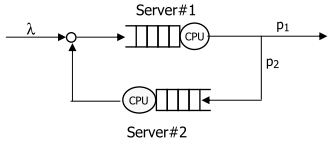
\includegraphics[scale=1]{figures/ex/jksnet.png}
\caption{Jackson Network}
\end{figure}
\end{center}

Si assuma che i singoli intervalli di tempo durante i quali viene utilizzato la 
CPU del server\#1 ed i singoli intervalli di tempo durante i quali viene 
utilizzata la CPU del server\#2 siano descritti da variabili casuali indipendenti 
e distribuite esponenzialmente a valor medio, rispettivamente, $\frac{1}{\mu_1}$ e $\frac{1}{\mu_2}$.  
Si assuma, inoltre, che i sistemi a coda in figura abbiano una capacità 
illimitata ed una disciplina di servizio di tipo FCFS.  
Si calcoli: 

\begin{itemize}
\item{a)} Il fattore di utilizzazione della CPU del server\#1; 
\item{b)} il valore medio del tempo di esecuzione di un job, a regime; 
\item{c)} il valore medio del tempo totale di CPU del server\#1 richiesto da un job, a 
regime; 
\item{d)} il valore medio del tempo totale di CPU del server\#2 richiesto da un job, a 
regime.

\end{itemize}

Risoluzione:

($\lambda$-POISSON) processi degli arrivi. $p_1$ che il job sia eseguito; $p_2=1-p_1$ che utilizzi il server 2. Se il job utilizza il server 2 ritorna in feedback all'ingresso di "1". $\{\{\lambda\},\{\mu_1,\mu_2\}\}$. $(d=+\infty)$, FCFS. Ci troviamo dinanzi una JN con code $\mathord{\cdot}$/M/1. Ma potrebbero anche essere \{$\mathord{\cdot}$/M/m, $\mathord{\cdot}$/M/$\infty$\}. M/M/1 in isolamento ai fini della OD. Definiamo con $\lambda_1$ velocità totale di arrivo dei clienti al nodo "1". Analogamente per "2", con $\lambda_2$. Applicando le equazioni del traffico troviamo:

\[
	\left\{
	\begin{aligned}
	&\lambda_1=\lambda+\lambda_2\\
	&\lambda_2=\lambda_1 p_2
	\end{aligned}
	\right. \implies \left\{
	\begin{aligned}
	&\lambda_1=\frac{\lambda}{1-p_2}\\
	&\lambda_2=\frac{\lambda}{(1-p_2=p_1)}p_2
	\end{aligned}
	\right.
\]

Dobbiamo imporre le Stabilità dei sottosistemi: $\implies$

\[
	\left\{
	\begin{aligned}
	&[\underline{\rho_1=\frac{\lambda_1}{\mu_1} = \frac{\lambda}{p_1\mu_1}}] < 1\\
	&[\underline{\rho_2=\frac{\lambda_2}{\mu_2} = \frac{\lambda p_2}{p_1\mu_2}}] < 1
	\end{aligned}
	\right.
\]

ove i termini sottolineati rappresentano il fattore di utilizzazione del server 1 e quello del server 2, rispettivamente. \underline{Little}. $\bar{N}=\bar{N}_1+\bar{N}_2$. Dove:

\[
	\left\{
	\begin{aligned}
	&\bar{N}_1 = \frac{\lambda_1}{\mu_1-\lambda_1} = \frac{\lambda}{p_1(\mu_1-\frac{\lambda}{p_1})} = \frac{\lambda}{p_1\mu_1-\lambda}\\
	&\bar{N}_2 = \frac{\lambda_2}{\mu_2-\lambda_2} = \frac{\lambda p_2}{p_1(\mu_2-\frac{\lambda p_2}{p_1})} = \frac{\lambda p_2}{p_1\mu_2-\lambda p_2} = \frac{\lambda}{\frac{p_1}{p_2}\mu_2-\lambda}
	\end{aligned}
	\right.
\]

Ricordiamo che $\lambda$ è la velocità totale di arrivo dei clienti dall'esterno. Dobbiamo quindi applicare Little: $\implies$ 

\[
	\bar{R} = \frac{\bar{N}_1+\bar{N}_2}{\lambda} = (\frac{1}{p_1\mu_1-\lambda} + \frac{1}{\frac{p_1}{p_2}\mu_2-\lambda})
\]

Quindi questo è il tempo medio di risposta. Dal punto di vista del tempo medio di risposta = tempo medio di permanenza, vi è un'equivalenza a due M/M/1 posti in serie, con velocità di servizio rispettivamente $\mu_1'=p_1\mu_1$ e $\mu_2'=\frac{p_1}{p_2}\mu_2$. RITARDO MEDIO il MEDESIMO, ma la distribuzione $\Pr\{R\leq t\}$ è DIFFERENTE!!

Calcoliamo le Service demand per i due nodi:

\[
	\left\{
	\begin{aligned}
	&D_1 = (\frac{1}{\mu_1}){(e_1=\frac{\lambda_1}{\lambda})} = \frac{1}{\mu_1} \frac{\lambda_1}{\lambda} = \frac{1}{\mu_1} \frac{\lambda}{p_1 \lambda} = \frac{1}{\mu_1 p_1}\\
	&D_2 = (\frac{1}{\mu_2})(e_2=\frac{\lambda_2}{\lambda}) = \frac{1}{\mu_2}\frac{\lambda p_2}{p_1}\frac{1}{\lambda} = \frac{1}{\mu_2}\underline{\frac{p_2}{p_1}}
	\end{aligned}
	\right.
\]

Dove $e_i$ rappresenta il numero medio di visite dall'esterno al nodo "i". Nel caso "2" ad esempio, il termine sottolineato indica $e_2 = \frac{p_2}{p_1}$. Notiamo che il nodo "1" verrà visitato sempre una volta in più prima di lasciare la rete: $+1 \implies \frac{p_2}{p_1}+1 = (\frac{1}{p_1})$. Potrei considerare: $\xi$ il numero totale di visite al server 1. $i-1$ volte visiti il nodo "2", e la volta successiva il cliente lascia la rete. Se $p_1=\Pr\{si\ lasci\ la\ rete\}$, allora vale:

\[
	\E[\xi] = \sum_{i=1}^{+\infty}{i\Pr\{\xi=i\}} = \sum_{i=1}^{+\infty}{ip_2^{i-1}p_1} =
\]
\[
	= p_1\sum_{i=1}^{+\infty}{ip_2^{i-1}} = p_1 \frac{1}{(1-p_2)^2} = p_1 \frac{1}{p_1^2} = \underline{\frac{1}{p_1}}
\]

(INDEPENDENT BERNOULLI TRIALS).


\subsection{Reti BCMP}

Reti di code \{CICLICHE, ACICLICHE, JACKSON\}. Per queste tipologie di code si ha una sola classe di clienti. Rete dati modellabile come rete di code, ma bisognerebbe differenziare le varie classi! $p_{ij} = \mathord{\cdot}(stream\ di\ pacchetti)$. Indici di prestazioni: \{ritardo medio\}. \underline{Reti di code BCMP} e teorema \underline{BCMP}. Va a definire una classe di reti di code per le quali vale ancora la Soluzione in forma prodotto per la Occupancy Distribution. Ma in questo caso i fattori del prodotto non corrispondono necessariamente alle distribuzioni marginali. Ma i fattori si ottengono a partire dall'analisi dei vari sistemi a coda visti in isolamento. Le BCMP comprendono le reti di JACKSON e quindi anche le ACICLICHE. C'è la possibilità di avere più classi di clienti $R$.

\begin{itemize}

\item{-)} $R=\cardinality{classi}$. Le classi possono essere APERTE o CHIUSE.

\begin{itemize}

\item{\textbf{APERTE}}: i clienti al loro interno possono partire dall'esterno ed arrivare dall'esterno;
\item{\textbf{CHIUSE}}: altrimenti
\end{itemize}

La BCMP è detta \textit{MIXED} se alcune classi sono aperte ed altre chiuse;

\item{-)} class switching possibile. Possibile che un cliente appartenente ad una certa classe, partendo da un nodo, visiti un certo nodo cambiando la sua classe;
\item{-)} $N=\cardinality{nodi}$. $p_{ir,js},\ r,s=1,2,\ \dots,\ (R=\cardinality{classi}),\ i,j=1,2,\ \dots,\ N=\cardinality{nodi}$ di reti di code. Si definirà quindi una \textit{matrice di routing}:

\begin{defn}{\textbf{Matrice di Routing}}

Per indicare le probabilità che un cliente appartenente ad una certa classe, partendo da un nodo, visiti un certo nodo cambiando la sua classe, si definisce:

\[
	\underline{\underline{P} := [p_{ir,js}]}
\]

\end{defn}

Tipicamente è una matrice SPARSA. A rigore sarebbe in realtà un tensore quadridimensionale. Se togliamo il class switching il tensore si ridurrebbe a 3 dimensioni.

\item{-)} Per quanto concerne la disciplina di coda, sino ad adesso abbiamo visto la FCFS, adesso ne sono consentite altre: \{\{PS, LCFS-PR, IS\}, FCFS\}. Ne spieghiamo qualcuna:

\begin{itemize}

\item{\textbf{PS} = \textit{processor sharing}}: \underline{tutti i clienti sono serviti contemporaneamente}, con time slicing;
\item{\textbf{LCFS-PR} = \textit{Last-Come-First-Served with Preemptive-Resume}}: Se un cliente viene servito ed arriva un altro cliente, vi è l'interruzione del servizio corrente ed il cliente corrente va in fila di attesa. Rientrerà nel servizio quando $\nexists$ clienti nel sistema a coda;
\item{\textbf{IS} = \textit{Infinite Server}}: Come suggerisce lo stesso nome, prevede INFINITI $(\infty)$ servitori! $\iff (m=+\infty)$ Come nell'M/M/$\infty$.

\end{itemize}

\end{itemize}

Vi è un'altra differenza (caratteristica aggiuntiva) riguardo la distribuzione dei tempi di servizio. Fino ad adesso abbiamo visto la distribuzione esponenziale. Adesso è permessa qualsiasi distribuzione purché la trasformata di Laplace della PDF sia razionale. COX ha dimostrato che qualunque distribuzione di v.a. si può approssimare sufficientemente bene mediante le seguenti reti di stadi: abbiamo una Rete di Stadi esponenziali. Il tempo di permanenza di un cliente in $\mu_i$ è distribuito esponenzialmente. Possiamo associare delle variabili casuali $\{\eta_1,\eta_2,\ \dots,\ \eta_n\}$ che sono tutte distribuite esponenzialmente $\iff \eta_i \sim EXP(\mu_i)\ \forall i=1,\ \dots,\ n$, ed indicano il tempo di permanenza in ciascuno stadio $i$-esimo. $\{a_i,b_i\}$ sono delle probabilità. La distribuzione associata all'attraversamento (al tempo di attraversamento) dell'intero sistema si chiama \textit{distribuzione di COX} e mediante essa possiamo approssimare (giocando opportunamente con il numero di stadi) sufficientemente bene una qualsiasi distribuzione. A questo punto il vincolo della trasformata di Laplace razionale della PDF non è più limitativo dal momento che la distribuzione di COX ha una TL della PDF razionale (PDF associata alla v.a. tempo di attraversamento).

Quindi possiamo pensare ad un unico servitore che rappresenti tutto il sistema. Il servitore è unico! Il servizio parte quando entra nel sistema e finisce quando il cliente esce dall'ultimo stadio. Solo alla fine un altro cliente va al servizio. In alcuni casi è ammessa una velocità del servizio che dipenda dal numero di clienti nella coda (M/M/m), o dal numero di clienti di una CERTA CLASSE nella coda.

(Probabilità di routing). La disciplina NON è a priorità! Ancora non la stiamo esaminando (interruzioni e senza interruzioni). Per queste reti che prevedono le forme prodotto NON è possibile.
Consideriamo il caso di rete BCMP aperta (\textit{OPEN-BCMP}). Vediamo che i processi degli ARRIVI sono ammesssi in questa rete. Consideriamo due casi, due possibilità:

\begin{itemize}

\item{\textit{\underline{CASO 1}}}: i clienti arrivano alla rete da un'unica sorgente, con tempi di interarrivo indipendenti e distribuiti esponenzialmente. Il Rate di arrivi $(\lambda)$ può dipendere dal numero di clienti $K$ nella rete $\iff \lambda=\lambda(K)$. \underline{Se $[\lambda\neq\lambda(K)]$} (si riferisce al rate di arrivo), \newline
\underline{avremo un processo di POISSON omogeneo}. Un cliente in arrivo visiterà il nodo $i$ in classe $r$ con probabilità $p_{0,ir}$ (giungendo dall'esterno). Ovviamente dovrà valere il seguente vincolo:

\[
	[\sum_{i=1}^N{\sum_{r=1}^R{p_{0,ir}=1}}]
\]

\item{\textit{\underline{CASO 2}}}: Se non facessi delle semplificazioni dovrei trattare delle sottocatene di Markov ergodiche. Eviteremo quindi il class switching. Supponiamo che non vi sia CS quindi. In tal caso si ha un processo degli arrivi $\forall$ classe di clienti. La velocità di arrivo $\lambda_r$ (indicizzata su $r$) potrà dipendere da $K_r \implies \lambda_r=\lambda_r(K_r),\ r=1,2,\ \dots,\ R$. Se $\lambda_r\neq\lambda_r(K_r)$ avremo un processo di POISSON omogeneo per la classe $r$.
\end{itemize}

Con le BCMP si può benissimo modellare un \textit{J2EE}, con Studio di Affidabilità e Disponibilità annesso. Quindi nel \underline{primo} caso abbiamo un unico processo degli arrivi, mentre nel \underline{secondo caso} non abbiamo class switching ed abbiamo un processo degli arrivi differente $\forall$ classe della rete. $K_r=\cardinality{clienti\ della\ classe\ r}$. Tipi di nodi ammessi nella BCMP: Nodi: \{\underline{type 1}, \underline{type 2}, \underline{type 3}, \underline{type 4}\}.

\begin{itemize}

\item{\underline{type 1}}: FCFS node. Coda con tempi di servizio distribuiti esponenzialmente con lo stesso valor medio (SAME $\frac{1}{\mu_i}$) per tutte le classi. La velocità di servizio $(\mu_i)$ può dipendere dal numero di clienti totali nella coda (nel sistema a coda). LOAD DEPENDENT SERVICE-RATE (LDSR) possibile. Può servire per modellare dispositivi I/O, HDD. Lo utilizzeremo per modellare tempi di accodamento e trasmissione dei router. Considereremo quindi: \{$\mathord{\cdot}$/M/$m_i$, \underline{FCFS}\};

\item{\underline{type 2}}: PS node (processor sharing). Utilizzato per modellare le CPU. Code con servitore unico e disciplina PS. Tutti i clienti sono serviti contemporaneamente. Sono possibili distribuzioni dei tempi di servizio diverse per classi diverse. Differenza rispetto al type 1. E qui non ci deve essere per forza l'esponenziale \{\underline{DSD} for \underline{DSC}\}. Vale sempre il vincolo sulle TL della PDF dei tempi di servizio. La velocità di servizio per una classe può dipendere dal numero di clienti nel nodo od anche dal numero di clienti di quella classe nel nodo. (Anche qui LDSR possibile);

\item{\underline{type 3}}: Detto IS (\textit{Infinite Server}) node oppure \textit{Delay Node}, perché solitamente utilizzato per modellare il ritardo (ritardo di elaborazione). Tutto quello scritto per il \underline{type 2} vale anche per il \underline{type 3}. Code del tipo: $\mathord{\cdot}$/G/$\infty$. Sempre un servitore a disposizione. In fila di attesa NON c'è mai nessuno. (Infiniti servitori $\implies \nexists$ fila di attesa). \`E come se non ci fosse alcuna disciplina;

\item{\underline{type 4}}: LCFS-PR (LCFS with Preemptive Resume). Coda con un unico servitore con quella disciplina di servizio. Contempliamo quindi le \{$\mathord{\cdot}$/G/1 - LCFS-PR\}. Unico servitore con quella disciplina di coda.

\end{itemize}

\subsubsection{Teorema BCMP}

Andiamo direttamente ad una versione semplificata del teorema BCMP (\textit{Baskett, Chandy, Muntz and Palacios}). Versione semplificata. Serve per modellare le reti di dati. Consideriamo BCMP (reti di code) aperte con load independent arrival rate. Quindi sostanzialmente processi di arrivo omogenei. Reti BCMP aperte con $[\lambda\neq\lambda(K)] \implies$ processi degli arrivi omogenei sostanzialmente.

Consideriamo che le velocità di servizio siano tali che $[\mu_i\neq\mu_i(K)]$. Casi ovviamente estendibili. Consideriamo:

\[
	\left\{
	\begin{aligned}
	&N=\cardinality{nodi}\\
	&R=\cardinality{classi}\\
	&K_i=\cardinality{clienti\ totali\ nel\ nodo\ i}\\
	&K_{ir}=\cardinality{clienti\ di\ classe\ r\ nel\ nodo\ i}\\
	&\underline{K}=(K_1,K_2,\ \dots,\ K_N)\\
	&\left\{
	\begin{aligned}
	&K_i=\sum_{r=1}^R{K_{ir}}\\
	&K=\sum_{i=1}^N{K_i} = \sum_{i=1}^N{\sum_{r=1}^R{K_{ir}}}
	\end{aligned}
	\right.
	\end{aligned}
	\right.
\]

Con queste quantità, la Occupancy Distribution è uguale a:

\[
	\Pr\{\underline{K}\} = \pi(K_1,K_2,\ \dots,\ K_N) = \prod_{i=1}^N{\pi_i(K_i)}
\]

questa è la OD per questa OPEN-BCMP. $\pi_i(K_i)$ è caratterizzato in questo modo:

\[
	\pi_i(K_i) = \left\{
	\begin{aligned}
	&\underline{(1-\rho_i)\rho_i^{K_i}},\ type\ 1,\ type\ 2,\ type\ 4\\
	&\e^{-\rho_i}\frac{\rho_i^{K_i}}{K_i!},\ type\ 3
	\end{aligned}
	\right.
\]

Per quanto concerne l'equazione che presenta il termine sottolineato, è bene specificare che abbiamo una restrizione sul type 1: è necessario avere esclusivamente un unico servitore ($\underline{m_i=1\ \forall i}$). La formula ricorda tanto la M/M/1. Ma vale anche per type (1,2,4). Reti: $\mathord{\cdot}$/M/$(1=m_i)$. Per la terza invece abbiamo reti $\mathord{\cdot}$/G/$\infty$. $\rho_i$ è il fattore di utilizzazione del nodo $i$. Vale: $\rho_i := \sum_{r=1}^R{\rho_{ir}}$. ($\forall$ classe di servizio), Se ho $m_i$ servitori nel type 1, $\pi_i(K_i)$ avrà la stessa espressione trovata per la M/M/$m_i$ $(\lambda_i,\mu_i)$. Le velocità di arrivo le calcoliamo con le \underline{EQUAZIONI DEL TRAFFICO}. Considerando $(m_i=1)$, dobbiamo imporre che $(\rho_i<1)$ per la STABILIT\`A della CODA. Anche per il type 1 con più servitori $(m_i\geq 1)$, avremo: $\rho_i=\frac{\lambda_i}{m_i\mu_i}$ nel caso $m_i\geq 1$. Quindi:

\[
	\rho_{ir} = \left\{
	\begin{aligned}
	&\frac{\lambda_{ir}}{\mu_i},\ type\ 1,\ \mu_i\neq\mu_{ir}\\
	&\frac{\lambda_{ir}}{\mu_{ir}},\ type\ \{2,3,4\},\ (\mu_i=\mu_{ir}) = \mathord{\cdot}(IDX\ r)
	\end{aligned}
	\right.
\]

Nel secondo caso infatti (seconda equazione), le distribuzioni dei tempi di servizio possono essere differenti per le varie classi. Ricordiamo che vale: $[\underline{\lambda_i}=\sum_{r=1}^R{\lambda_{ir}}]$, differenziando ed includendo rispetto alle varie classi.  Il termine sottolineato rappresenta la velocità \underline{totale} di arrivo al nodo $i$.

\subsection{RECAP}

[BCMP $\supset$ JACKSON $\supset$ ACICLICHE]. $\pi_i(K_i)$, reti \{$\mathord{\cdot}$/M/1, $\mathord{\cdot}$/G/1-PS, $\mathord{\cdot}$/G/1-LCFS-PR\}. Per queste code, ai fini dell'Occupancy Distribution, si comportano come se fossero delle M/M/1 in isolamento ($1=m_i$ servitori $\forall i$). Nel type 1 abbiamo la FCFS, mentre nel type 2, type 4 non abbiamo quella disciplina di coda! \`E come se ai fini del calcolo della OD, avessimo invece proprio la disciplina FCFS. Si comportano proprio come se fossero M/M/1 in isolamento.

Per quanto riguarda il secondo caso, per un M/M/$\infty$ abbiamo $[\e^{-\rho_i}\frac{\rho_i^{K_i}}{K_i!}]$. Ma vale sostanzialmente per tempi di servizio non distribuiti esponenzialmente (per le $\mathord{\cdot}$/G/$\infty$). La motivazione è collegata proprio al teorema BCMP. Tornando al primo caso, ipotizziamo una rete di code BCMP con un processo degli arrivi dall'esterno che NON dipenda dal carico (Stiamo considerando un processo degli arrivi di POISSON omogeneo). Il BCMP vale anche se c'è un solo sistema a coda! Consideriamo $\mathord{\cdot}$/M/1. Adesso sono sicuro che mi trovo dinanzi una M/M/1. Adesso i processi degli arrivi sono di POISSON. Per il \underline{type 2}, M/G/1-PS. Stesso discorso per il \underline{type 4}. Le formule trovata per un M/M/1, sono valide anche per un \{\underline{M/G/1-PS}, {M/G/1-LCFS-PR}\}, ove i termini sottolineati si riferiscono rispettivamente a code del tipo \underline{type 2} e \underline{type 4}.


\section{Reti di dati}

Ulteriore passaggio verso la modellazione. Obiettivo: modellare una rete di dati switched. Consideriamo $(i\rightarrow j)$. Ci saranno 4 componenti di ritardo su questo link. Dobbiamo considerare:

\begin{itemize}

\item{-)} tempi di accodamento in $i$;
\item{-)} tempi di trasmissione su questo link;
\item{-)} tempi di propagazione;
\item{-)} tempi di elaborazione

\end{itemize}

Modellando queste componenti di ritardo per il link $(i\rightarrow j)$, consideriamo nel primo blocco sicuramente $\mathord{\cdot}$/M/1 e agli ultimi due blocchi utilizzeremo rispettivamente: \{$\mathord{\cdot}$/G/$\infty$ e $\mathord{\cdot}$/G/$\infty$\}.
I sistemi a coda sono dei modelli per modellare il ritardo.

Virtual Circuit (a commutazione di pacchetto). Per un certo flusso la ROTTA sarà sempre la stessa. Stiamo immaginando qui di avere 3 flussi: $\{X_{s1}, X_{s2}, X_{s3}\} \leftarrow$ velocità di arrivo. Per il link $(i\rightarrow j)$ abbiamo il flusso di pacchetti $s_1-s_2 \implies X_{s_{i-j}} = X_{s1}+X_{s2}$. A questo punto, per valutare $\lambda_{ij}$, dobbiamo trovare la somma delle $X_s$ estesa a tutti gli stream $S$ che attraversano il link $(i\rightarrow j)$:

\[
	[\underline{\lambda_{ij}} = \sum_{stream\ s\ in\ (i,j)}{X_s}]
\]

$X_{si}$ è il rate (velocità) del flusso $i$-esimo. La rete Internet è a commutazione di pacchetto ma di tipo Datagram (Rotte non sempre le stesse). Per le DATAGRAM: $f_{ij}(s_1)X_{s,1}$ rappresenta la Velocità di arrivo, considerando le opportune frazioni dei pacchetti. Qui per calcolare le velocità di arrivo totale dobbiamo considerare le seguenti formule:

\[	
	\underline{\lambda_{ij}} = \sum_{stream\ s\ in\ (i,j)}{f_{ij}(s)X_s}
\]

ove la somma è estesa al solito a tutti gli stream che attraversano il link $(i\rightarrow j)$. Biforcazione o fork possibile.

Velocità di arrivo totale dei vari link sia su una VC che su una DATAGRAM. Entrambe a commutazione di pacchetto. Rete di code BCMP. Versione semplificata del teorema per modellare una rete di dati come una rete di code. Modellare ogni link della rete con il seguente schema:




Ipotesi sul sistema reale. Rete BCMP (più flussi) $\implies$ ($\forall$ flusso $\exists$ classe associata ad esso $\iff (s\rightarrow r)$). Sia $R=\cardinality{flussi\ di\ pacchetti}$. Rete BCMP con $R$ classi di clienti. Consideriamo il generico flusso $s$, al quale corrisponde una certa velocità $X_s \impliedby (s\rightarrow X_s)$. Per quanto concerne le velocità totali abbiamo: $\underline{\lambda_{0,r}}$ è la velocità di arrivo dall'esterno dei clienti di classe $r$; $\lambda_{0,hr}$ è la velocità di arrivo dall'esterno dei clienti di classe $r$ alla coda di ingresso $h$ della rete; $p_{0,hr}$ è la probabilità che un cliente dall'esterno di classe $r$ vada verso la coda $h$. Immaginiamo che $h$ sia il nodo di ingresso $\implies p_{0,hr}=1$:

\[
	X_s=\lambda_{0,r} \impliedby [\lambda_{0,r}p_{0,hr} = \underline{\lambda_{0,hr}}]
\]

Difatti quella probabilità è 1 per quella coda che rappresenta il nodo di ingresso. $\nexists$ biforcazioni all'ingresso della rete. Per applicare il teorema BCMP dovremo imporre che questi pacchetti arrivino secondo un processo di POISSON. Un'altra ipotesi riguarda i tempi di trasmissione. Nel primo blocco modelliamo il ritardo di accodamento e quello di trasmissione. Dobbiamo ipotizzare che i tempi di trasmissione siano distribuiti esponenzialmente (Con la stessa distribuzione per tutte le classi). Parametro $(\frac{1}{\mu_{ij}})$ come valor medio. Supponiamo che i buffer del router siano molto grandi $(d=+\infty)$ da poter ritenersi illimitati. Valga l'approssimazione di Kleinrock. Indipendenza tra i tempi di interarrivo e tempi di servizio. (Reti magliate ed intensità di traffico medio-alta). Vale quando la rete è abbastanza magliata e intensità di traffico medio-alta. Con queste ipotesi possiamo applicare il teorema BCMP. I due successivi blocchi di ritardo modellano il tempo di propagazione e di elaborazione (quest'ultimo è il router $j$) (ADN). Per elaborazione si intende il ritardo per decidere il routing. Il router analizzerà i vari link e si occuperà di decidere consultando le tabelle di forwarding. Il tempo di propagazione si trascura solitamente. Al posto dell'$\mathord{\cdot}$/M/1 andrebbe bene un $\mathord{\cdot}$/M/$\infty$. Anche se non siamo vicini alla distribuzione esponenziale per le lunghezze dei pacchetti, tutto alla fine va ancora bene. Applichiamo quindi le formule BCMP. Sia: $\bar{R}$ il tempo medio di attraversamento della rete da parte di un pacchetto. \underline{POOLING} di tutti i flussi che attraversano lo stesso link. Abbiamo: $\bar{R}=\frac{N}{\gamma}$, ove abbiamo posto $\gamma:=\sum_{tutti\ gli\ stream\ s}{X_s}$ ovvero la velocità totale di arrivo dei pacchetti. Dato che abbiamo a che fare con valor medi... indichiamo inoltre con \{$\E[T_{ij}^p],\ \E[T_{ij}^e]\}$ rispettivamente il valor medio del tempo di propagazione ed il valor medio del tempo di elaborazione, entrambi sul link $(i\rightarrow j)$. Sfruttando le formule dell'M/M/1 e di Little otteniamo:

\[
	\bar{N}_{ij} = \frac{\lambda_{ij}}{\mu_{ij}-\lambda_{ij}} + \lambda_{ij}\E[T_{ij}^p] + \lambda_{ij}\E[T_{ij}^e]
\]

Abbiamo trovato il numero medio di pacchetti sul link $(i,j) \implies \bar{N}=\sum_{(i,j)}{\bar{N}_{ij}}$. Dividiamo per la velocità totale di arrivo dei pacchetti $(\gamma)$ e troviamo $\bar{R}$. Sempre per il fatto della forma prodotto. (M/M/1) in isolamento (BCMP TH.). Se introduco un modello M/G/$\infty$, un po' di errore lo commetto. Le formule che ottengo per l'M/G/$\infty$ sono analoghe a quelle M/M/$\infty$.

\begin{thrm}{\textbf{$\bar{R}_{path}$}}

Per calcolare questa quantità, dovrei considerare tutti i link associati a questo percorso:

\[
	\bar{R}_{path} := [\sum_{link(i,j)\ lungo\ path}{\frac{1}{\mu_{ij}-\lambda_{ij}}}] + \E[T_{ij}^p + \E[T_{ij}^e]]
\]

\end{thrm}

Vale per tutte le classi! $(\forall r=s)$. Qualunque sia la sua classe. Tanto è inglobata nelle varie quantità $(\mu_{ij},\ \lambda_{ij})$. 


\subsection{Exercise}

Consider the network in the figure below. There are four sessions: ACE, ADE, BCEF and BDEF 
sending Poisson traffic at rates $\{100,\ 200,\ 500,\ 600\}\ pkt/min$, respectively. Packets lengths are 
exponentially distributed with mean $1000\ bits$. All transmission lines have capacity $50\ kbits/s$, 
and there is a propagation delay of $2\ msec$ on each line. Using the Kleinrock independence 
approximation, 

\begin{itemize}

\item{a)} find the average number of packets in the system, the average delay per packet (regardless of 
session) and the average delay per packet of each session; 
\item{b)} derive the CTMC that can be used to find the approximate delay distribution related to the 
packets belonging to the ACE session

\end{itemize}

\begin{center}
\begin{figure}[H]
\centering
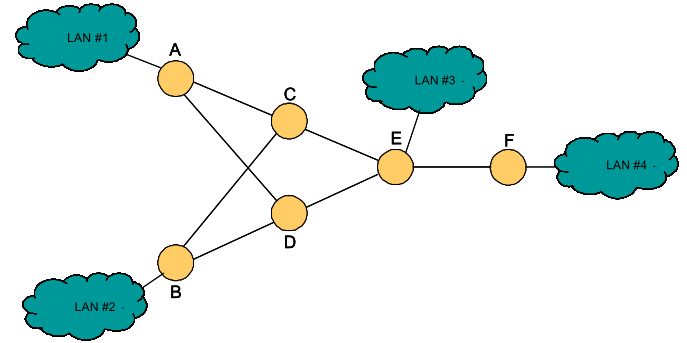
\includegraphics[scale=0.8]{figures/ex/mdn.png}
\caption{Data Network}
\end{figure}
\end{center}

Flussi in realtà bidirezionali. Ma a livello didattico concentriamoci nel caso NON DUPLEX ($\iff$ Flussi unidirezionali). Abbiamo varie sessioni:

\[
	\left\{
	\begin{aligned}
	&ACE, 1\\
	&ADE, 2\\
	&BCEF, 3\\
	&BDEF, 4
	\end{aligned}
	\right.
\]

Quattro servizi che generano pacchetti alle seguenti velocità. $\{100,200,500,600\}\  [pkt/min]$. $\mathit{L}=1000\ bit$ (lunghezza pacchetti), $C=50\ kbps$. $\E[T_{ij}^p]=dp=2ms$ (propagation delay, PD). ($\forall ij$. Qualunque sia il link $i,j$). Il PD è in realtà una costante, non un valor medio. Supponiamo quindi che tutti i link siano alla stessa velocità. Supponiamo valida l'approssimazione di Kleinrock. 4 flussi di pacchetti $\iff$ 4 sessioni di comunicazioni. Numeriamo le sessioni e calcoliamo:

\[
	\left\{
	\begin{aligned}
	&X_1 = (\frac{100}{60} = \frac{5}{3})\ pkt/s\\
	&X_2 = (\frac{200}{60} = \frac{10}{3})\ pkt/s\\
	&X_3 = (\frac{500}{60} = \frac{25}{3})\ pkt/s\\
	&X_4 = (\frac{600}{60} = 10)\ pkt/s
	\end{aligned}
	\right.
\]

Ci serve andare a calcolare le velocità totali di arrivo sui VARI link attraversati. 

\[
	\left\{
	\begin{aligned}
	&\lambda_{AC}=X_1\\
	&\lambda_{CE}=X_1+X_3=10\ pkt/s\\
	&\lambda_{AD}=X_2\\
	&\lambda_{BD}=X_4=10\ pkt/s\\
	&\lambda_{DE}=X_2+X_4=\frac{40}{3}\ pkt/s\\
	&\lambda_{BC}=X_3\\
	&\lambda_{EF}=X_3+X_4=\frac{55}{3}\ pkt/s
	\end{aligned}
	\right.
\]

Dobbiamo andare a considerare la velocità di servizio su ogni link. Ci troviamo dinanzi $\mathord{\cdot}$/M/1. Ma anche relativi ai router dei blocchi $\mathord{\cdot}$/G/$\infty$. Dividiamo $\frac{C}{\mathit{L}}=\mu_{ij}=(\frac{50000}{1000}=50)\ pkt/s$. Dobbiamo calcolare il $\gamma$ (velocità totale di arrivo dei clienti):

\[
	\gamma=\sum_{i=1}^4{X_i}=\frac{70}{3}\ pkt/s
\]

in quanto abbiamo 4 flussi diversi. Con $\bar{N} \simeq 1.84\ pkt$ pacchetti, abbiamo quindi:

\[
	\bar{R}=\frac{\bar{N}}{\gamma}=\frac{1.84}{70/3\ pkt/s} = \frac{3(1.84)}{70} msec\ (millisec)
\]

(poco credibile oggi). Dobbiamo ora calcolare il ritardo medio $\forall$ stream (per i vari stream). Per le varie sessioni ($\bar{R}_{path}$ formula), abbiamo:

\[
	\bar{R}_p=[50ms,\ 53ms,\ 87ms,\ 90ms]
\]

$\Pr\{R\leq t\}$, dove $R$ è il ritardo, tempo di attraversamento della rete.

Distribuzione del ritardo. Supponiamo di voler determinare la distribuzione del ritardo dei pacchetti associati alla sessione ACE. CMTC che con uno stato assorbente può essere utilizzata per modellare il ritardo $(ACE=AC+CE)$ (link attraversato):



Distribuzione di ritardo = tempo di permanenza di un pacchetto nella rete in questione. Abbiamo trascurato i ritardi di elaborazione. $\mathord{\cdot}$/M/1, che tiene conto dei ritardi di accodamento + il ritardo di trasmissione. Presso il nodo "C" arriveranno pacchetti anche dal nodo "B" (da un altro stream) (BCEF). Determinare la distribuzione del tempo di risposta in una rete di code aperta. C'è un metodo per approssimare questa distribuzione (del tempo di risposta), e si basa sulla conoscenza della distribuzione del tempo di risposta relativa ai vari sottosistemi di cui la rete si compone. Reti di code di JACKSON. Tempo di risposta = tempo di attraversamento. Vogliamo approssimare questa distribuzione (del tempo di risposta). \`E possibile andare a derivare da questa rete di JACKSON una CMTC con \underline{stato assorbente}. Il \underline{time-to-absorption} (la sua distribuzione), rappresenta un'approssimazione del tempo di risposta della rete. Se è ACICLICA (rete di JACKSON senza CICLI) si ha una coincidenza tra TTA e tempo di risposta della rete.
Consideriamo questa rete CICLICA:

\begin{center}
\begin{figure}[H]
\centering
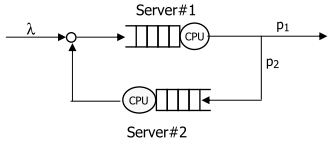
\includegraphics[scale=1]{figures/ex/jksnet.png}
\caption{Jackson Network}
\end{figure}
\end{center}

Due $\mathord{\cdot}$/M/1. Questo metodo si basa sulla conoscenza delle distribuzioni dei vari tempi di risposta dei singoli sottosistemi di cui si compone la rete. M/M/1. $R$ = tempo di permanenza. Sappiamo che: $R \sim EXP(\mu-\lambda)$. $F(t)\ CDF$, quindi la CDF del tempo di risposta in un M/M/1 è:

\[
	F(t)=\Pr\{R\leq t\} = 1-\e^{-(\mu-\lambda)t}
\]

Sulla base di queste conoscenze, possiamo dedurre, ricavare la seguente CMTC:

\begin{center}
\begin{tikzpicture}[->, >=stealth', auto, semithick, node distance=3cm]
\tikzstyle{every state}=[fill=white,draw=black,thick,text=black,scale=1]
\node[state]    (1)                     {$1$};
\node[state]    (2)[right of=1]   {$2$};
\node[state]    (C)[below of=1]   {$C$};
\path
(1) 
    edge[bend left]     node{$(\mu_1-\lambda_1)p_2$}     (2)
    edge[bend right,left]    node{$(\mu_1-\lambda_1)p_1$}      (C)
(2) edge[bend left]                node{$(\mu_2-\lambda_2)\underline{1}$} (1);
\end{tikzpicture}
\end{center} 

con: $\{\{C\},\{1,2\}\}$ rispettivamente come Stato assorbente e Stati transitori. Lo STARTING STATE è lo stato 1, ovvero lo stato dalla quale evolve la CMTC. $R\sim EXP(\mu-\lambda)$. Rappresenta la permanenza del cliente sul sistema. Tempo di permanenza di un determinato cliente. In particolare, il tempo di soggiorno della CMTC in questo stato corrisponde al tempo di permanenza nel primo M/M/1. ($R_1\sim EXP(\mu_1-\lambda_1)$). Il tempo di soggiorno della catena nello stato 2 rappresenta il tempo di permanenza del cliente nel sistema nel sistema a coda 2 ($R_2\sim EXP(\mu_2-\lambda_2)$). Se invece lasciasse la rete, si avrebbe una transizione verso lo stato assorbente \{C\}. Il TTA qui corrisponde al ritardo del cliente in questa rete (tempo di permanenza). Se riesco a determinare la distribuzione del TTA per questa catena riesco a determinare proprio il tempo di permanenza nella mia rete. Ma è un'approssimazione questa, in quanto abbiamo dei cicli! Quindi i processi degli arrivi NON sono di POISSON. 

\[
	\underline{\Pr\{T_a\leq t\}} \simeq \underline{\Pr\{R\leq t\}}
\]

ove il LHS sottolineato rappresenta $\pi_C(t)$ in TRANSITORIO, mentre il RHS sottolineato rappresenta la distribuzione del ritardo nella mia rete. A quanto pare vi è un'approssimazione possibile. Per trovare $\pi_C(t)$ si può procedere con il metodo della trasformata di Laplace, diversamente ci sono dei programmi di simulazione e non. Si richiami il concetto di affidabilità:

\[
	\Pr\{R>t\} = 1-\underline{\pi_0(t)} = 1-\Pr\{R\leq t\}
\]

\subsection{Response-Time Blocks (RTB)}

Li utilizziamo per trovare queste distribuzioni. Blocchi mediante i quali costruiamo le CMTC con stati assorbenti. Dobbiamo considerare tanti blocchi quante sono le componenti di ritardo.

\begin{itemize}

\item{\textbf{RTB \textit{M/M/1}}}: Ci sono quindi anzitutto quelle per la M/M/1 $(\lambda,\mu)$, ove per stabilità deve valere: $(\lambda<\mu)$. Il RTB per questo sistema è il seguente:

\begin{center}
\begin{tikzpicture}[->, >=stealth', auto, semithick, node distance=3cm]
\tikzstyle{every state}=[fill=white,draw=black,thick,text=black,scale=2]
\node[state]    (IN)                     {$IN$};
\node[state]    (OUT)[right of=IN]   {$OUT$};
\path
(IN) edge[bend left]     node{$(\mu-\lambda)$}     (OUT);
\end{tikzpicture}
\end{center}

Lo stato IN rappresenta il fatto che il cliente è entrato nella coda. Il tempo di soggiorno nello stato \{IN\} rappresenta il ritardo nella rete. \{OUT\} = \{partenza del cliente nella coda\}. (Tante serie di blocchi quanti sono i nodi in gioco):

\[
	\underline{F(t)} = 1-\e^{-(\mu-\lambda)t}
\]

Ove il termine sottolineato rappresenta la CDF del tempo di risposta. Lo stato \{OUT\} rappresenta la partenza del cliente. OUT nel precedente esercizio era \{2,C\}=OUT. In tali casi saranno da pesare le velocità di uscita complessive (con probabilità eventualmente, corrispondenti alle cosiddette probabilità di routing);

\item{\textbf{RTB \textit{M/M/$\infty$}}}: Il tempo di soggiorno nella mia catena corrisponde al tempo di servizio $\iff \nexists$ code nella M/M/$\infty$. (infiniti servitori, NO fila di attesa). 

\begin{center}
\begin{tikzpicture}[->, >=stealth', auto, semithick, node distance=3cm]
\tikzstyle{every state}=[fill=white,draw=black,thick,text=black,scale=2]
\node[state]    (IN)                     {$IN$};
\node[state]    (OUT)[right of=IN]   {$OUT$};
\path
(IN) edge[bend left]     node{$\mu$}     (OUT);
\end{tikzpicture}
\end{center}

Tempo di risposta corrisponde al tempo di servizio:

\[
	F(t) = \Pr\{R\leq t\}=1-\e^{-\mu t}
\]

\{IN\} rappresenta quindi lo stato di permanenza nel mio sistema;

\item{\textbf{RTB \textit{M/M/m}}}:

Per ultimo, ma non di importanza, abbiamo l'RTB di una M/M/m:

\begin{center}
\begin{tikzpicture}[->, >=stealth', auto, semithick, node distance=3cm]
\tikzstyle{every state}=[fill=white,draw=black,thick,text=black,scale=2]
\node[state]    (IN)                     {$IN$};
\node[state]    (OUT)[right of=IN]   {$OUT$};
\path
(IN) edge[bend left]     node{$\frac{\mu m (1-\rho)}{m(1-\rho)+C}$}     (OUT);
\end{tikzpicture}
\end{center}

ove $C$ è la C di ERLANG, ovvero la probabilità di accodamento;

\end{itemize}

Ma lo stato OUT può corrispondere allo stato IN di un altro blocco! Se effettivamente OUT è l'uscita della rete sarà assorbente, altrimenti NO.

Adesso consideriamo la rete precedente. Quella è la rete di code che modella la sessione ACE sostanzialmente:

\begin{center}
\begin{tikzpicture}[->, >=stealth', auto, semithick, node distance=3cm]
\tikzstyle{every state}=[fill=white,draw=black,thick,text=black,scale=1]
\node[state]    (A)                     {$A$};
\node[state]    (AC)[right of=A]   {$AC$};
\node[state]    (C) [right of=AC]                    {$C$};
\node[state]    (CE)[right of=C]   {$CE$};
\node[state]    (OUT)[right of=CE] {$OUT$};
\path
(A) edge[bend left]     node{$\mu-\lambda_AC$}     (AC)
(AC) edge[bend left]     node{$\frac{1}{d_AC}$}     (C)
(C) edge[bend left]     node{$\mu-\lambda_CE$}     (CE)
(CE) edge[bend left]     node{$\frac{1}{d_{CE}}$}     (OUT);
\node at ($(OUT)+(0,-0.8)$) {stato ASSORBENTE};
\end{tikzpicture}
\end{center}

Il nodo E interfaccia i pacchetti verso la LAN 3. (\underline{Rete ACICLICA}). Trascuriamo il ritardo di elaborazione, al solito. Velocità elevatissima! A volte si può ritenere legittimo trascurare il ritardo di accodamento e trasmissione della LAN di destinazione! Molto veloce! TTA in tal caso coincide esattamente con il ritardo di attraversamento (tempo di attraversamento) della rete, dal momento che la rete è ACICLICA.

%************************************************
% Chapter 5: NETWORK TECHNOLOGIES 2
%************************************************
% !TEX encoding = UTF-8
% !TEX TS-program = pdflatex
% !TEX root = ../nt.tex
% !TEX spellcheck = it-IT

%************************************************
\chapter{Network Technologies 2}
\label{cap:nt2}
%************************************************\\

\section{(Rapid)STP - Spanning Tree Protocol}

\{M/M/1, M/M/$\infty$\}. (STP)$\rightarrow$(RSTP) rapida. La RSTP (Rapid) è la versione veloce dell'STP. \`E un protocollo che consente di trasformare una topologia magliata in una ad albero (bridge). L'STP porta a dei tempi di convergenza molto elevati. \textit{IEEE 802.1D} è lo standard che va a definire i \textit{Transparent Bridge}. Oggi i bridge sono HW (lvl 2). Prima erano a livello SW. Oggi abbiamo i router HW ASIC elettronici (matrici ASIC).

L'STP serve per evitare che vi siano dei loop a lvl 2. Queste maglie esisteranno per via dei link ridondanti, introdotti per aumentare l'Affidabilità/Disponibilità. Dato che gli switch/bridge IEEE 802.1D non tollerano topologie magliate, allora serve l'STP. Il pericolo è quando loro fanno il flooding. Fase di forwarding, MAC Multicast/Broadcast $\implies$ flooding su tutte le altre porte. MAC Unicast $\implies$ funzioni di forwarding, previa consultazione delle sue tabelle di forwarding/routing. Si possono creare dei LOOP ad esempio, con il flooding. Tante copie dello stesso pacchetto. Gli switch lvl 2 NON tollerano topologie magliate. Una rete Fault-Tolerant richiede invece topologie magliate. Ma alla fine dobbiamo avere quella ad albero. Switched LAN. $\forall$ porta $\exists!$ LAN. Come l'STP si occupa di effettuare questa trasformazione? Trasforma alcune porte dello switch in \textit{BLOCKING}, altre in modalità \textit{FORWARDING}. Ogni interfaccia dello switch è numerata. Una porta bloccata non potrà forwardare/ricevere trame $\iff$ No elaborazione. Esiste anche lo stato \textit{DISABLED}. Quando è disabilitata, è come se non ci fosse proprio nella topologia ai fini dell'STP. Disabilitata quando o c'è un guasto, o viene disabilitata da un \textit{Network Manager} oppure non è collegata a nessun dispositivo. Esistono anche switch remoti! Che interconnettono LAN geografiche. A scala geografica ci potrebbe essere un enorme spreco, se disabilitassimo alcune porte. Link di comunicazine geografici $\implies$ bridge remoti. Se NON utilizzassimo un link geografico, avremmo un notevole spreco di banda. DRAWBACK. Le path risultanti dall'STP potrebbero essere più lunghe rispetto ad altre path che si potevano scegliere. L'STP converge via via in caso di guasti a nuovi ST (\textit{Spanning Tree}). Switched LAN = reti LAN interconnesse tra switch. Quando c'è qualche guasto, alcune altre porte che stavano in Blocking potrebbero tornare in Forwarding. Con le nuove convergenze riusciamo a farle comunicare.

\subsection{Funzionamento STP}

Modi di funzionamento: tre fasi principali. \underline{Alta Disponibilità} $\implies$ rete fault-tolerant $\implies$ ridondanza. VLAN (\textit{Virtual LAN}). Se le VLAN attraversassero più piani in tal caso, ci sarebbe bisogno dell'STP. Cosa accade quando una VLAN rimane confinata in un solo piano/od attraversa più piani? RSTP possibile. Abbiamo tre fasi principali:

\begin{itemize}

\item{\textit{Elezione del \textbf{ROOT BRIDGE}}}: $\exists!$ "highlander", root bridge. Tutte le porte del root bridge saranno settate a \underline{forwarding};
\item{\textit{Selezione della \textbf{ROOT PORT}}}: $\forall$ bridge $\neq$ root, seleziono la porta verso la quale giunge a costo minimo al \underline{root bridge}. La ROOT PORT di ogni bridge viene settata in FORWARDING;
\item{\textit{Selezione del \textbf{BRIDGE DESIGNATO} e della \textbf{DESIGNATED PORT}}}: $\forall$ segmento LAN alla quale saranno collegati due o più bridge, viene selezionato un bridge detto \textit{BRIDGE DESIGNATO}. Sarà quello più vicino al ROOT BRIDGE. La porta del bridge designato con la quale quel bridge è collegato a quel segmento viene detta \textit{PORTA DESIGNATA}. Solo il BRIDGE DESIGNATO sarà autorizzato ad inoltrare le trame dati!

\end{itemize}

 Un segmento LAN. LAN = rete locale che si basa su un canale Broadcast (canale ad accesso multiplo ad accesso circolare). Si risolve col protocollo MAC (Nell'Ethernet abbiamo il \textit{CSMA/CD}). Il canale è a diffusione circolare ma la trasmissione non sarà inviata in Broadcast. Sentiranno tutti ma lo elaborerà solo uno quel determinato pacchetto. Una stazione è un dispositivo che implementa almeno il sottolivello MAC. Un ripetitore NON è una stazione! (Implementa solo il Physical). Anche il ROOT BRIDGE è collegato a segmenti LAN. Ma tutte le sue porte sono in Forwarding $\implies$ tutte le porte del root bridge sono designate. La porta designata sarà ovviamente messa in stato di Forwarding. $\forall$ segmento abbiamo il bridge designato. 

Perché funzioni l'STP abbiamo bisogno di scambiare dei messaggi di controllo (BPDU) - \textit{Bridge Protocol Data Unit}. Parliamo di un protocollo standardizzato dall'ISO. Problema del supporto multiprotocollo. Ogni livello ha il problema del multiprotocollo (es. LLC per 802.1). Ma l'IP non è stato standardizzato dall'ISO $\implies$ serve lo SNAP. Codici per l'LLC abbiamo 042H sia per il DSAP che il SSAP. \`E l'LLC che trasporta la BPDU. Le BPDU possono essere di due tipi:

\begin{itemize}

\item{\textbf{\textit{Configuration BPDU}}} utilizzata per la definizione della topologia loop-free (ad albero);
\item{\textbf{\textit{Topology Change Notification BPDU} (TCN BPDU)}} con l'obiettivo di scatenare nuovamente l'STP per far convergere ad un nuovo albero;
\end{itemize}

Il campo \textit{BPDU type} fa la differenza tra i due tipi \{CONFIG, TCN\}. Quelle di CONFIG hanno anche altri fondamentali campi dell'STP. \{TC/ \dots /TCA\}. servono per lo scatenamento delle reazioni alle notifiche TCN (C)BPDU $\implies$ hello messages!

\begin{itemize}

\item{\textit{Root Bridge ID}}: identificativo del bridge che \newline \underline{si assume} sia il ROOT BRIDGE \{REAL/SUPPOSED\}, per via della presenza di una fase transitoria;
\item{\textit{Root Path Cost}}: Path a minor costo verso il root bridge a partire dallo switch che sta trasmettendo questo messaggio di configurazione. Inviato ovviamente NON significa che l'abbia generato lui!
Messaggi di Hello = CBPDU. Costo della path a minor costo;

\item{\textit{Bridge ID}}: identificativo del transmitting bridge;
\item{\textit{Port ID}}: analogamente per questo transmitting bridge: la porta dalla quale STA INVIANDO il messaggio;
\item{\textit{\{Message Age, Max Age, Hello Time, Forward Delay\}}} sono impostati dal ROOT BRIDGE. Nell'\textit{Hello Time} imposterà il tempo di inter-ricezione dell'hello message. Di default pari ad (1s). Ogni 1s hello time da parte del root bridge. Passato l'hello time si aspetta un altro \textit{Max Age}. Scaduto anche questo tempo, manda delle TCN BPDU. Forward delay (default 15s);

\end{itemize}

Identificativi (IDS):

\begin{itemize}

\item{\textit{\textbf{Bridge Identifier e Root Identifier}}}: (\textit{Bridge Priority + Bridge MAC Address}). Di default la priorità è settata a 32768. Viene settata (incrementata o decrementata a steps di 4096 unità);
\item{\textit{\textbf{ID di porta}}}: (\textit{Port priority + Port number}). default 128 la priorità. Passi di 16 unità possibili. Dividiamo in due la rappresentazione decimale (es. 128.21). 1 byte per la priorità ed 1 byte per il numero di porta;
\end{itemize}

\{Root ID, Bridge ID, Port ID\}. Poi avevamo il Root Path Cost. Alla porta di uno switch è associato un costo, settato manualmente da un Network Manager oppure sono dei costi raccomandati dalla IEEE, a seconda della velocità della porta (es. Ethernet). 16 bit per il costo. Fino a 65535 (Unsigned). Fino a 10Tb/s. (Revised \textit{802.1D}) (Switched LAN). Alle porte sono associate dei costi. Un bridge sarà in grado di calcolare il root path cost a partire dalle porte sulle quale sta ricevendo. Costo porta di ricezione + costo che troviamo nel messaggio di hello. Additività. Bisognerà preoccuparsi ovviamente di aggiornare via via il Root Path Cost per inviare a valle (ad un livello più basso della topologia).

\subsubsection{Spiegazione FASI STP}

\begin{itemize}

\item{1)} Elezione del ROOT BRIDGE. Parte la rete. Ogni switch pensa di essere il root bridge. Nel Root Path Cost metteremo ovviamente 0! Root ID = Bridge ID inizialmente. Se un bridge riceve su una certa porta un messaggio di Hello, farà un confronto con il proprio Root ID. Vince l'ID più basso! (Bridge ID più basso). Root/Bridge ID. Il bridge con maggior Bridge ID tra questi ora non invierà più messaggi di hello, e setterà il proprio Root Path Cost a partire dal costo della porta dalla quale sta ricevendo. Se la priorità è lasciata di default, il confronto verrà fatto a livello di indirizzo MAC. In questo modo $\exists!$ alla fine Root Bridge, con il (Bridge ID) = (Root ID) più basso. Prima di forwardare un messaggio di hello, un bridge non root modificherà opportunamente il Root Path Cost. Alla fine uno soltanto sarà eletto. ID: \{Bridge Priority + Bridge MAC\}. Ad uno switch è associato un indirizzo MAC. Avrà un MAC $\forall$ porta. Per la sua operatività non serve il MAC in realtà. Per quanto riguarda le trame dati difatti, gli indirizzi MAC sono \underline{trasparenti}! Da qui il nome \underline{\underline{TRANSPARENT BRIDGE}}. Prima abbiamo l'elezione del \underline{Root Bridge};

\item{2)} fase successiva: elezione della \underline{Root Port}. $\forall$ bridge non root dovrà selezionare la Root Port. $\exists$ certa sequenza di condizioni che devono essere verificate in caso di condizioni di parità:

\begin{itemize}

\item{-)} Supponiamo che si verifichi una situazione di parità sulla porta (Rotta a minor costo);
\item{-)} Selezioniamo come Root Port quella sulla quale i messaggi hanno il Bridge ID più basso;
\item{-)} Se abbiamo stessi Bridge ID abbiamo il confronto con la Port ID. Porta dalla quale si riceve il messaggio di hello con il più piccolo Port ID. Porta di INVIO. Porta tramite la quale quel transmitting bridge sta inviando il messaggio di hello;
\item{-)} Alla fine si passa alla quarta condizione discriminante: identificativo della porta di ricezione. Vince quella minore;
\end{itemize}

La prima condizione prevede la discriminante come Least Cost (Root Path Cost);

\item{3)} Selezione della PORTA DESIGNATA. $\forall$ segmento LAN ci sarà da selezionare un bridge designato. Quale sarà il bridge designato? Quello che sta comunicando su quel segmento LAN delle BPDU a più basso costo;

\end{itemize}

Se una porta è bloccata NON vi è inoltro. Un Hub (ripetitore) è come se non ci fosse (è trasparente per loro). Un hub NON potrebbe interconnettere LAN a differenti velocità, né LAN a differenti MAC (avrebbe bisogno dello stack data layer a lvl 2). Ci sarebbe inoltre bisogno dello \textit{STORE \& FORWARD} (S\&F). Quest'ultimo lo possono fare switch, router (logica di elaborazione lvl 2, lvl 3).

Alla fine sarà il Root Bridge ad inviare messaggi di hello. Valori dettati dal Root Bridge. Se un Bridge non root si aspetta di ricevere messaggi di hello con quella temporizzazione, aspetta un pochino di tempo (pari a Max Age). Passato anche questo tempo (tipicamente 20s), il suddetto bridge scatena l'STP, mandando TCN. Se una porta, prima in stato di Blocking (per evitare i loop), deve passare a Forwarding, tutto ciò non avviene immediatamente. Prima quella porta viene messa in \textit{LISTENING STATE} per evitare loop. Quella porta si potrebbe accorgere che il Root Bridge è "obsoleto". Passato un quantitativo di tempo pari a Forward Delay, entra in \textit{LEARNING STATE}, nella quale sarà autorizzata ad utilizzare il \textit{Backward Learning}. Dopo un altro tempo pari al Forward Delay, finalmente la porta entrerà in \underline{\textit{Forwarding State}}. Durata massima (pensando ai tempi di default), $20+15+15=50s$. Si è quindi definito l'RSTP. Se avessimo più switch naturalmente avremmo dei transitori molto lunghi, e questi valori temporali potrebbero essere pesanti, soprattutto se si parla di una rete di grandi dimensioni! Potrebbe creare lei stessa dei loop. Pericolo di \textit{Broadcast Storm} (invocazioni troppo frequenti dell'STP):

TCA settati (\textit{Topology Change Acknowledgements}) dal notifier del cambiamento della topologia. Modifica dell'Aging Time (Apprendimento Annullato). La convergenza è pesante, ed è stata risolta \underline{dall'RSTP}. \textit{IEEE 802.1AX}. Raggruppare link paralleli tra stazioni. Quattro link a $100\ Mbit/s$ ad esempio. Raggruppare ad un link logico con banda più o meno costante (grossomodo $400\ Mbit/s$) (LACP) = \textit{Link Aggregation Control Protocol}. In parallelo NON abbiamo il problema della convergenza (non se ne accorgerà l'STP). Il costo del Link cambierà ad un guasto, aumenterà di preciso. Il costo del Link Logico invece diminuisce al raggruppamento. Il protocollo lavora soltanto con Full-Duplex alla stessa trasmissione.

RSTP = \textit{Rapid STP}, definito nell'\textit{IEEE 802.1W}. Lavora come l'STP, ma cambia la terminologia: \textit{Discarding} $\supset$ \{Blocking, Listening, Disabled\}. Si può scendere giù di 10s, oppure di 12 o 2s in alcuni casi. Con l'STP abbiamo la selezione della Root Port. Se una root port viene meno, viene scelta la porta \textit{Alternative} a minor costo. Meccanismi aggiuntivi che lo rendono molto più veloce. Se ci sono degli Hub Repeater ivi prevediamo solo dei link punto-punto! Altrimenti stessi tempi dell'STP;

Agire sulla topologia modificando il campo \textit{Priorità}.

VLAN = Virtual LAN. Configurare su una Switched LAN diverse sotto-LAN logiche. Configurazione LAN virtuali. Differenti VLAN comunicano tra di loro solo sfruttando il lvl 3. L'STP non andrà a guardare le LAN virtuali. Prima avevamo quindi l'esecuzione di una sola istanza dell'STP. Per effettuare \textit{Load Balancing} si è introdotto l'MST (\textit{Multiple STP}). C'è da pensare a vari parametri $\forall$ VLAN (Virtual LAN). Quindi è stato modificato il campo Bridge Priority (primi 16 bit). Bridge ID: (Priority ID + Bridge MAC). BP non più di 16 bit. 12 bit = identificativo della VLAN. 4 bit più a monte: valore effettivo della priorità. Il campo di 16 bit è stato quindi diviso in 2: 32768 default priority. Incrementi consigliati sempre di 4096. (4 bit = BP + 12 bit = \textit{System ID Extension}). 4 bit $\implies$ 16 valori di priorità possibili. Non è comunque limitativo. L'intero Bridge Priority sarà quindi modificato MA sarà comunque da affiancare all'indirizzo MAC per formare il Bridge ID ed eventualmente Root ID.


\subsubsection{RECAP}

STP. Strategie per evitare che un malintenzionato possa collegarsi ad uno switch di piano ed alterando la BPDU con priorità molto basse, modificando quindi lo Spanning Tree. Oltre ad alterare lo Spanning Tree potrebbe anche intercettare il traffico. Se lui fosse il ROOT, il traffico transiterebbe tutto verso di lui. Potrebbe di conseguenza anche creare una situazione DoS. Due opzioni, proposte in ambito CISCO:

\begin{itemize}

\item Configurare \textit{fast port} (generalmente user port), ma non va bene perché toglierebbe la possibilità di avere un PC con meccanismi di switching;
\item \textit{Root Guard} disabilita una porta che diventerebbe STP root port;

\end{itemize}

L'STP di default è sempre attivo sugli switch. Si può disattivare ma è meglio tenerlo prevalentemente attivo.

All'avvio di una rete switchata parte l'STP a lavorare (vedasi \textit{Cisco Packet Tracer}). Di default sugli switch lvl 2 o multilayer è configurato sulla VLAN 1 (sulla quale sono associate tutte le porte). ID Bridge: \{Priorità + Indirizzo MAC\}. Con l'avvento delle VLAN adesso abbiamo la suddivisione della Priorità in: \{BPV: \textit{Bridge Priority Value} di 4 bit + \textit{System ID Extension}\} $\leftarrow$ relativo al Multiple Spanning Tree (MST). Gli ultimi 12 bit sono l'identificativo delle VLAN. es. Bridge Priority: 32769: priorità effettiva: 32768 + (1 = VLAN ID). Link punto-punto. Costo 19 porte \textit{Fast Ethernet}. Se cambiamo priorità, l'algoritmo si riavvia. Bisogna specificare la VLAN. Ci vuole un certo tempo perché converga l'algoritmo (STP).

\section{LAN Virtuali (VLAN)}

Un'organizzazione ha bisogno di avere LAN parallele (indipendenti). Come realizzarle? Si utilizzino degli apparati come switch per collegare le varie stazioni interessate ai rispettivi switch. La tecnologia delle LAN virtuali consente questa configurazione a livello SW, mediante VLAN, anche se i dispositivi sono fisicamente collegati. Una certa serie di VLAN può esserci anche con un singolo switch, con un'operazione opportuna di configurazione. Ma le stazioni LAN potrebbero non essere separate fisicamente! Sono separate logicamente. Potrebbero anche esserci due o più switch $\implies$ le VLAN in questo caso si estendono su più switch $\iff$ stazioni collegate a switch diversi fanno parte della stessa VLAN. VLAN che si estendono su più piani, su più switch. Essenzialmente una VLAN è un dominio di \textit{BROADCAST} $\neq$ dominio di \textit{COLLISIONE}. Nel primo se una stazione trasmette un pacchetto in broadcast, nonostante tutti possano sentirlo, un meccanismo di arbitraggio virtuale del canale fa in modo che giunga a destinazione e venga elaborato solo da uno. Si ricordi che uno switch è una stazione! (Almeno lvl 2). \{Stazioni = Router, Host, Switch\}. Attraverso il full-duplex il MAC è bypassato. \`E lo switch che stabilisce il dominio di BROADCAST. Gli switch separano i domini di collisione. Se tutte le stazioni di una LAN fossero collegate ad un Repeater, allora otterremmo un unico dominio di collisione, più grande, che coincide in tal caso con il dominio di BROADCAST. Un dominio di BROADCAST contiene uno o più domini di collisione.

Una LAN virtuale corrisponde ad un dominio di BROADCAST. Possiamo già pensare ad una motivazione per le VLAN. Contenere le dimensioni dei domini di broadcast. Far fronte ai protocolli \textit{Broadcast Intensive} (ARP utilizza il Broadcast, ma non è BI!). Altre motivazioni: VLAN per raggruppare gli utenti in Gruppi di Lavoro. Esigenza di avere LAN separate $\iff$ motivazioni di sicurezza. Evitare che il traffico di una certa serie di utenti transiti, riguardi altre VLAN. Due VLAN comunicano tra di loro solo se vi è un dispositivo lvl 3 che le interconnette (router IP con Subnet IP). Controllano il traffico mediante le ACL, diversamente le due VLAN non potrebbero comunicare.
Conflitto di competenze: Mantenere dispositivi sensibili, importanti su una LAN virtuale. Separare determinate tipologie di traffico. \textit{Telecommunication Outlet} nella stessa stanza. Si sfrutta un'unica presa di rete (es. telefono VoIP con L2 switch incorporato). Questioni di convenienza (es. TAG VLAN). Nel TAG ci saranno i Campi di \textit{Priorità}. Marcatura a lvl 2, parlando di priorità delle trame appartenenti ad un certo flusso.


Si aggiunge un cosiddetto \textit{Tag} per le VLAN. Sorta di francobolli che identificano la VLAN alla quale la stazione appartiene. Sulla base di questi tag lo switch ricevente capirà come gestirlo. Un link tra due switch attraverso il quale viaggiano trame taggate viene chiamato \textit{TRUNK}. E le porte agli estremi del collegamento si chiamano \textit{porte TRUNK}.

Configurazione di VLAN. Operazione di configurazione. Ci sono due tipologie di porte: \{\textit{ACCESS}, \textit{TRUNK}\}:

\begin{itemize}

\item{\textbf{\textit{Access}}}: Le prime trasmettono e ricevono trame NON taggate. Una porta ACCESS potrà gestire una sola VLAN alla quale essa corrisponde. Tipicamente alle porte access ci collego gli host;
\item{\textbf{\textit{Trunk}}}: A queste porte invece possono essere configurate differenti VLAN. A quale VLAN è permesso attraversare la linea trunk è deciso in fase di configurazione;
\end{itemize}

La VLAN 1 è quella di default e $\forall$ port $\in$ VLAN 1. La VLAN nativa normalmente corrisponde alla VLAN 1, e le trame associate alla VLAN nativa NON sono taggate! Anche le ACCESS in realtà possono collegare due switch. Associazione: \{porte $\leftrightarrow$ VLAN\}. Un link trunk tra due switch può essere sempre sostituito con $n$ link access, ove $n$ è il numero di VLAN che viaggiano normalmente sul link trunk. Link Access associato alla VLAN. In questi casi NON abbiamo più trame taggate, ma ci stiamo giocando $n$ link! E costano un bel po' sugli switch. 

\subsection{Configurazione}

Configurazione. Comandi CISCO:

\begin{lstlisting}[language=CISCO]
show VLAN brief
\end{lstlisting}

VLAN1 = VLAN di default. Per aggiungere delle VLAN devo anzitutto crearle:

\begin{lstlisting}[language=CISCO]
Sw#vlan database
Sw(vlan)#vlan 2 name Ammin
VLAN 2 added:
	Name: Ammin
\end{lstlisting}

Si creino le nuove VLAN. Dopodiché dobbiamo cominciare ad associare le porte:

\begin{lstlisting}[language=CISCO]
Sw(config)#int GigabitEthernet 0/1
Sw(config-if)#switchport access vlan 2
Sw(config-if)#exit
\end{lstlisting}

Porta di tipo ACCESS associata alla VLAN 2. Per la modalità trunk invece, nel link trunk viaggeranno trame taggate:

\begin{lstlisting}[language=CISCO]
Sw(config)#interface GigabitEthernet 0/1
Sw(config-if)#switchport mode trunk
Sw(config-if)#switchport trunk allowed vlan 1,4,5
Sw(config-if)#exit
\end{lstlisting}

Prima entriamo nell'interfaccia delle porte ovviamente. Di default le porte sono tutte ACCESS per la VLAN 1. Oppure:

\begin{lstlisting}[language=CISCO]
Sw(config-if)#switchport trunk allowed vlan all
\end{lstlisting}

Le reti \textit{Token Ring} sono state create dall'IBM, ma non ebbero molto successo per via dei costi elevati. Preferibile oggigiorno l'Ethernet perché più semplice con il suo potentissimo CSMA/CD.

Standard che specificano le LAN virtuali: \textit{IEEE 802.1Q - 2005}. VLAN specificate da questi standard. Ma questi standard prevedono le VLAN per porta (\textit{Per-port VLAN}). Tutte le stazioni collegate allo switch mediante quelle porte faranno parte alle VLAN associate a quelle porte. Si abbassa però la Flessibilità. Richiede un certo peso per il Network Manager. Bassa flessibilità su maggior controllo da parte del Network Manager. I produttori possono anche fornire soluzioni alternative, ma non rispettano ovviamente gi standard i quali servono per interoperare invece. L'802.1-Q specifica anche il formato per il tag, i quali servono per identificare la VLAN di appartenenza quando i pacchetti attraversano i link trunk. Il TAG consiste in 4 byte. 2 byte \textit{Type/Length} che si differenziano sulla base dell'\textit{IEEE 802.3}. Per il PADDING serve il Length. Per far sì che la trama abbia una certa lunghezza minima.

[64,1518] byte. Il TAG consiste in 4 byte (2 byte + 2 byte). Primi 16 bit (2 byte) TPID (\textit{Tag Control Protocol Identifier}); se codice 81-00 significa che dopo vi sarà il Tag della VLAN: TCI (\textit{Tag Control Information}) $\supset$ \{PCP (\textit{Priority Code Point}): priorità della trama a lvl 2 per la QoS. 7 livelli di priorità: Il 7 è il più alto, mentre il più basso è l'1, mentre quello 0 è di default. Tramite questa priorità si differenzia il servizio fornito; DEI (\textit{Drop Eligible Indicator}) di 1 bit. Qualora si verifichino fenomeni, situazioni di congestione, sono i primi frame (quelli preferibili, candidati) a venire scartati; \textit{VLAN} ID (VID), valore di 12 bit. Le VLAN sono numerate da 1 a 4095 (esattamente 4095 VLAN diverse possibili). Ma il VID può valere anche 0 (quella trama NON è associata a nessuna VLAN). Quel TAG è stato scritturato solo per fornire priorità alla trama (nel PCP)\}. La VLAN 1 è spesso utilizzata per una VLAN di gestione (\textit{management VLAN}). I vari apparati dovranno ovviamente essere gestiti.

L'\textit{IEEE 802.1-V} va invece a definire le VLAN per protocollo. Si immagini di configurare un protocollo ad una VLAN. Lo switch, ricevendo una trama, va a vedere la rispettiva PDU. Prevale la IEEE 802.1-V su quella Port-Based. Prima avevamo un solo \textit{Filtering Database}. Adesso i moderni switch supportano l'IVL (\textit{Independent Virtual LAN}): $\forall$ VLAN $\exists!$ Filtering Database. Con questa modalità possiamo associare ad una stazione più VLAN.

Configurazione link trunk. Transitano le trame relative a quelle VLAN permesse. MVRP (\textit{Multiple VLAN Registration Protocol}). Gli switch stessi capiscono quali trame VLAN possono transitare. In base alle VLAN che vi sono agli estremi. Può coesistere una situazione mista. Le trame che partono da una VLAN 1 NON sono taggate su un link trunk. Importante in alcuni scenari. Le BPDU viaggiano NON taggate! 

Più istanze STP. Originariamente si poteva creare una sola istanza dell'STP. L'STP NON vede le VLAN! Più recentemente si è data la possibilità di avere più istanze dell'STP $\rightarrow$ (MST) per \textit{Multiple Spanning Tree}. Decidere le associazioni VLAN - Spanning Tree. Tipicamente uno Spanning Tree può coinvolgere più VLAN quindi. Load balancing a lvl 2. \{PVST, PVST+\} sono protocolli proprietari Cisco. Mentre l'MST è uno standard. LO standard IEEE è comunque stato derivato dall'MST.

\subsection{Private Virtual LAN (PVLAN)}

LAN Virtuali. VLAN Private. Non vi sono degi standard dietro. I produttori si sono inventate le PVLAN. Molto utili. Suddividere una VLAN già esistente in ulteriori sottodomini di BROADCAST, sebbene le subnet IP rimangano sempre quelle di partenza. Ogni sottodominio ha una: \{VLAN Primaria, VLAN Secondaria\}. La primaria è condivisa da tutti i sottodomini. La VLAN secondaria è quella che fa la differenza. \`E costituita da \textit{Porte Isolate} che possono comunicare con le cosiddette \textit{Porte Promiscue}. Le \textit{Porte COMMUNITY} possono comunicare solo con le porte nella stessa Community VLAN e con le porte promiscue. \{porte promiscue\}: porte della VLAN primaria. Una porta promiscua può comunicare con tutte le porte: \{$\exists!$ VLAN ISOLATA $\land\ \exists$ VLAN COMMUNITY (multiple)\} $\leftarrow$ VLAN secondarie. \`E una tecnologia che gioca un ruolo importante nelle DMZ. Queste VLAN private possono estendersi su più switch. Esiste anche qui il concetto di link TRUNK. Suddivisione in sottodomini. Le porte promiscue le gioco per firewall, router. Attraverso le VLAN viaggiano le trame appartenenti alla stessa VLAN community.

\begin{itemize}

\item{-)} In una VLAN regolare il broadcast raggiunge tutte le porte della VLAN;
\item{-)} Si ricordi che le porte VLAN isolate comunicano soltanto alle porte promiscue, oppure alle porte trunk se esse permettono di raggiungere una porta promiscua. Le porte promiscue sono utilizzate per accedere al mondo esterno mediante router. Sul link trunk abbiamo il tagging. Accedendo verso una porta promiscua non abbiamo più bisogno di TAG (PVLAN).

\end{itemize}

Si ricordi che qui non abbiamo più il concetto standardizzato di \{ACCESS, TRUNK\}. Dominio delle PVLAN. I produttori si sono inventati questa furba tecnologia.

Quindi, per quanto riguarda il broadcast, adesso esso raggiunge solo porte isolate, link trunk (o porte promiscue). Mentre per il broadcast delle VLAN Community, essi raggiungono porte Community (della stessa community), link trunk ed al solito porte promiscue. Questa tecnologia bloccante a lvl 2 serve per proteggere interi blocchi lvl 2 di DMZ.

\section{NETWORK DESIGN}

Design di una rete di Campus ad Alta Disponibilità (\underline{High Availability}). Gli Access Point sono tipicamente Lite. Architettura basata sul controllore. Unico controllore per tutto il campus (SPoF e bottleneck). $\forall$ access point ho un tunnel verso un unico controllore. C'è un tunnel dall'access point al controllore. Unico tunnel. Possibilità di Controllo ridondante.

\subsection{Progettazione di rete ad Alta Disponibilità}

\begin{itemize}

\item{\textbf{Analisi dei Requisiti}}: Prima fase. Requisiti legati al Business di un'Azienda, alla Mission di un'Organizzazione. Requisiti tecnici: \{throughput, delay, delay jitter\} che consentono di ottenere gli obiettivi della mission. \{Disponibilità, Sicurezza dei Dati. Strettamente legati alla Disponibilità\};
\item Caratterizzare la rete esistente (che tipo di HW, SW è presente). Magari ci saranno delle applicazioni già presenti (flussi di traffico presenti, correnti e quelli futuri);
\item{\textbf{PROGETTAZIONE LOGICA}}: Topologia rete, protocolli di routing, strategia di sicurezza e strategia di management (http). Progettata logicamente la rete si passa al: 
\item{\textbf{livello fisico}}:

\begin{itemize}

\item Tecnologie e dispositivi per reti di campus;
\item Tecnologie e dispositivi per WAN.
\end{itemize}

Ci si può avvalere di programmi tipo Packet Tracer per testare il progetto della rete. Si possono (devono) ovviamente applicare delle variazioni in retroazione.

\end{itemize}

\subsection{FAULT-TOLERANCE}

Una rete può essere progettata per le performance, per la sicurezza, per la Disponibilità. Alcuni requisiti ovviamente vanno in conflitto tra di loro. Adesso ci occupiamo di \textit{Fault-Tolerance}. Bisogna pensare alla ridondanza. Abbiamo diversi tipi di Ridondanza:

\begin{itemize}
\item{\textit{Backbone}};
\item{\textit{Device}};
\item{\textit{ITB (In The Box)}};
\item{\textit{Interfaccia di Rete}};
\item{\textit{Stazione duale (tandem, watch dog)}};
\item{\textit{Sistemi Cluster}}
\end{itemize}

La soluzione fault-tolerant dev'essere la più semplice possibile. Ridondanza del default router. Molto importante! Sicuramente il router di default va ridondato! Il primo protocollo proposto ed utilizzato è l'HSRP (\textit{Hot Standby Router Protocol}) della CISCO (proprietario ovviamente). Poi abbiamo il VRRP, LGBP;

\subsubsection{HSRP}

L'HSRP fa sì che si crei un \underline{router virtuale} (detto anche router fantasma). L'\textit{Active Router} e lo \textit{Standby Router} sono router fisici! Il fantasma no! A quello fantasma corrisponde un indirizzo IP e MAC. Ogni host nella rete avrà come default gateway l'indirizzo di quello fantasma. Più di due router possibili, ma router attivi e standby saranno soltanto due! Tutti apparterranno allo stesso gruppo comune. $\exists$ FASE di elezione, basata sul concetto di priorità (100 di default). Qui il router con la più alta priorità diventa quello Attivo. In caso di parità, diventa Attivo quello con l'indirizzo IP più grande. Alla fine della fase di elezione, quello Attivo avrà il ruolo del router virtuale (fantasma), ed assumerà anche IP e MAC (indirizzi) di quello fantasma. Quindi l'interfaccia del router attivo avrà due indirizzi IP! Sempre lui dovrà rispondere alle richieste ARP per il router di default (Manderà la \textit{ARP reply}).

Al termine dell'elezione, periodicamente l'Attivo e lo Standby manderanno dei messaggi di hello. Se il router attivo va down, subentra lo standby come quello Attivo. Ma bisogna eleggere quello di standby tra i router del gruppo HSRP. Se cade quello di standby, di nuovo bisogna eleggerne un altro di standby. Ci saranno dei timer opportuni. I messaggi HSRP sono inviati all'IP multicast 224.0.0.2 sulla porta UDP 1985. Se appropriamente tunato, converge in 1 secondo. Il MAC del router virtuale può essere configurato manualmente oppure creato automaticamente come well-known. Per quanto riguarda l'indirizzo IP, bisognerà configurare opportunamente le interfacce dei router Standby ed Attivo:

\begin{lstlisting}[language=CISCO]
Router-X> interface ethernet 0
Router-X> ip address 10.1.1.1 255.255.255.0
Router-X> standby 24 ip 10.1.1.5
\end{lstlisting}

(24 è l'HSRP Group!) A questo punto la elezione che, si basa sull'indirizzo IP qualora la priorità sia la medesima, avrà sicuramente successo. Una volta che un router è diventato Attivo, non molla l'asso anche se subentra qualcuno migliore di lui (Priorità od IP). Ma può subentrare con la funzionalità \textit{preempt}, se opportunamente configurata con:

\begin{lstlisting}[language=CISCO]
Router-X> interface ethernet 0
Router-X> ip address 10.1.1.1 255.255.255.0
Router-X> standby 24 preempt
Router-X> standby 24 priority 105
Router-X> standby 24 ip 10.1.1.5
\end{lstlisting}

Naturalmente sono le interfacce che devono gestire il gruppo HSRP. Funzionalità \textit{TRACK}. Se entrambi i router (Standby ed Attivo) sono collegati in Seriale ad un altro router, e la tratta Active - Router $\mathit{Z}$ va in down, allora entra in funzione Track che va automaticamente ad abbassare la Priorità del Router "down":

\begin{lstlisting}[language=CISCO]
R-X>interface ethernet 0
R-X-if>ip address 10.1.1.5 255.255.255.0
R-X-if>standby 1 preempt
R-X-if>standby 1 priority 105
R-X-if>standby 1 ip 10.1.1.10
R-X-if>standby 1 track Serial 0
R-X-if>no shutdown 
R-X-if>exit
R-X>interface serial 0
R-X-if>ip address 10.6.2.5 255.255.255.0
\end{lstlisting}

Se va giù quell'interfaccia si diminuisce la priorità (di default vi sono decrementi di 10). Naturalmente si opererà sull'interfaccia. \textit{1} qui indica il relativo gruppo HSRP, mentre \textit{Serial 0} è l'interfaccia di interesse. La track ha senso ovviamente solo se c'è la Preempt!

\subsubsection{Multi-HSRP}

l'HSRP normale porta ad uno spreco della banda! Il Router di Standby NON è autorizzato a forwardare pacchetti IP che arrivano dagli host! Il router Standby non farà niente per instradare verso l'esterno! $\iff$ banda sprecata. I link geografici devono essere adeguatamente sfruttati. Sull'Internet ci sono dei protocolli di routing dinamici (ECMP - \textit{Equal Cost Multipath Routing}). Nelle tabelle di routing ci potrebbero essere path col medesimo costo. Load balancing. Con il \textit{multi-HSRP} faremo \textit{load Sharing} (Balancing). Un router può essere attivo per un gruppo e standby per un altro. Paradigma a stella. Per fare il Load Sharing bisognerà configurare opportunamente gli host, ovviamente. Operazione molto scomoda. Si utilizza nella pratica VLAN+DHCP. Si configuri lo switch con due VLAN (metà parte VLAN 10 e l'altra metà VLAN 20). Per-port VLAN. Le due VLAN corrispondono ad IP differenti. Stiamo pensando all'utilizzo del DHCP. Ovviamente i link switch-router saranno link TRUNK. Settare opportunamente le VLAN ID di appartenenza dopo l'accesso alle interfacce.

Attenzione ad utilizzare l'HSRP su reti switchate! Se va giù il link di comunicazione TRA switch ci sono problemi in entratata con l'ECMP. Sorgono dei problemi di irraggiungibilità (\textit{reachability problem}) per gli host. Il problema si risolve raddoppiando il link di comunicazione (facendo girare STP opportunamente per i loop), oppure si aggregano quei due in un unico link mediante LACP - Link Aggregation Control Protocol. \underline{\textit{IEEE 802.1AX}} per aggregare i link. Nella realtà non sono collegati questi switch! Ma sono messi in stack tra di loro.

Poi abbiamo il VRRP - \textit{Virtual Router Redundancy Protocol}. Definito in \textit{RFC 2338}. Molto simile all'HSRP (Master $\rightarrow$ Active, Slave $\rightarrow$ Standby); GLBP \textit{Gateway Load Balancing Protocol}. Ci consente di evitare il multi-HSRP. Si crea un unico gruppo GLBP, nel quale entreranno a far parte le interfacce. Unico gruppo. Tutti gli host saranno configurati con l'IP del virtual router. L'AVG (\textit{Active Virtual Gateway}) viene eletto, ed è lui l'elemento preposto a rispondere alle \textit{ARP Request}. In maniera ciclica (round-robin) verranno scelti i MAC dei restanti membri del gruppo, denominati AVP (\textit{Active Virtual Forwarder}). 

\subsubsection{Sicurezza in HSRP}

Problema della Security. Indirizzi IP multicast alla quale vengono mandati i pacchetti HSRP: 224.0.0.102 sulla porta UDP 1985. Problema della sicurezza dati. C'è la possibilità che venga sferrato un attacco DoS qualora vi sia \textit{Spoofing HSRP}. Stazione utilizzata da un hacker che manda dei pacchetti hello HSRP con priorità 255 (max priority). Molto probabile che esso diventi il router Attivo. Enhancement necessari. Di default lo schema di autenticazione è un testo in chiaro nel messaggio di hello. Il router accetta il pacchetto solo se corrisponde questo campo di \textit{Authentication}. Molto debole, soggetto a possibili sniffing. La stringa di default è "cisco". Ma un hacker potrebbe ugualmente sniffare con un \textit{Packet Sniffer}. Troubleshooter per problemi di rete, utile ai Network Manager. Switch lvl 2 (bridge). Per la trama broadcast e multicast esso farebbe un flooding. A lvl 2 ci sarebbe un MAC Multicast. Rilevazione trama + Spoofing. Supporto dell'\textit{IGMP Snooping} per le trame Multicast (hello HSRP nel messaggio IP). Ma con questo protocollo si riesce a capire mediante quale porta si riescono a raggiungere determinati gruppi multicast. Abbiamo un enhancement MAC (\textit{Message Authentication Code}) con MD5. Facciamo vedere i comandi rispettivamente quello di default e l'enhancement MD5:

\begin{lstlisting}[language=CISCO]
...
Router-X> interface ethernet 0
Router-X> ip address 10.1.1.1 2
Router-X> standby 24 authentication text string
Router-X> standby 24 authentication md5 key-string string
...
\end{lstlisting}


Ove 24 è al solito l'identificativo del gruppo HSRP. \textit{string} $\rightarrow$ password mediante la quale vengono hashati i messaggi (in questo caso gli hello HSRP). Possibile pure un filtraggio a livello MAC (switch avanzati). Access List a livello più basso (\textit{ACL lvl 2}). La versione HSRPv2 supporta l'MD5.

\subsection{Network Design in pratica}

Switched LAN. Rete ad alta disponibilità. Fault-Tolerant $\rightarrow$ Ridondanza. Abbiamo visto ridondanza sul default router. Ridondanza sulle dorsali verticali. Certo numero di piani. Su ogni piano, nel Telecommunication Closet (centro-stella di piano) ci si mette uno switch lvl 2 (switch di piano) che raccoglierà le istanze di piano. Switch di accesso. Poi abbiamo l'\textit{Equipment Room} (locale tecnico), ove abbiamo il centro stella di edificio (S1-P, S1-S). Apparati attivi nelle ER. La maggior parte dei flussi di traffico passa da qui. Bisogna quindi ridondare opportunamente. Devono essere abbastanza potenti! Poi abbiamo le dorsali verticali. Cavi, a rigore. LIU (\textit{Lightguide Interconnection Unit}). Apparati di centro-stella. \textit{CAVEDIO} (primaro \& secondario). Le due dorsali scorrono in cavedi differenti. I produttori consigliano di mettere negli ER degli switch multilayer (lvl 2 - lvl 3). Centro-stella. Apparati molto più potenti. Switch di distribuzione. \textit{Livello distribuzione}. Ridondanza sulle dorsali. Si creano dei possibili LOOP $\rightarrow$ STP $\rightarrow$ (R)STP ovviamente. Root bridge S1-P, ma interviene S1-S se malfunziona il primo. Modifica automatica della priorità (previo identificativo). In particolare si avrà il decremento della priorità. 32768 di default, a decrementi di 4096. Confronti sul Root Path Cost. Path a stesso costo $\implies$ link alla stessa velocità. Spanning-Tree.

Ridondanze sull'interfaccia (fault-tolerant). Si fa girare l'HA-Linux (High Availability). Si ha lo switching in automatico qualora l'interfaccia (una delle due) vada giù. Se va giù uno switch del lvl distribuzione, con questo sistema è tutto OK. Switch $\leftarrow$ bridge. Oggi gli switch sono in HW (ASIC). Pensare anche alla capacità elaborativa! Gli switch del livello distribuzione devono essere ben potenti. Utilizzo delle VLAN (LAN virtuali). Per far comunicare host appartenenti a VLAN differenti abbiamo bisogno necessariamente del lvl 3. Possibilità 3 porte access al posto di 1 trunk la quale richiederebbe che il router soprastante sia \textit{VLAN-Aware}. Link geografico che porta dal Router alla vera e propria Internet. Dobbiamo pensare anche eventualmente alla ridondanza dei link geografici. Pensare all'utilizzo dell'HSRP e del VRRP in questo caso. ECMP (Equal Cost Multipath Routing). Il discorso HSRP ha a che fare solo con il traffico in uscita. Pensare a più gruppi HSRP! ($\forall$ VLAN $\exists!$ HSRP), tipicamente.

Switch livello distribuzione lvl 2. Multi-layer switch. I router tradizionali lavorano non in hardware, ma con le CPU. I multilayer lavorano a lvl hardware! Matrice ASIC. I multilayer lavorano a lvl 3 come dei router! Lavorano in HW solo per il protocollo IP! Commutano ad altissima velocità a livello IP per reti di campus. Per i link geografici non ne avremmo bisogno (capacità trasmissiva bassa). Il multilayer lavora in HW per gli IP (maggioranza dei pacchetti). \{IPX, AppleTalk\} $\leftarrow$ legacy lvl 3 protocols. Multilayer switch. I router tradizionali vanno bene quando il $\cardinality{VLAN} \ll +\infty$, il traffico è basso e le ACL sono limitate.

\subsubsection{NO-FAULT TOLERANT NETWORK}

Immaginiamo che le varie entità organizzative siano disposte per piani, su reti differenti.

\begin{itemize}

\item Le VLAN non attraversano i piani. Associare ai vari piani differenti Subnet IP, configurate $\forall$ piano. Indirizzo IP specifico x piano (SW-1) multilayer. Non c'è bisogno che lavoriamo a lvl 2. Qui abbiamo domini di broadcast differenti. In questo caso non abbiamo bisogno che lavori a lvl 2 $\rightarrow$ lvl 3 $\leftarrow$ router. Router che fa L'Internetworking tra host associati alla stessa Subnet IP. Ogni interfaccia dà verso una rete fisica differente. Con un router normale andrebbe tutto bene! Ma con un multilayer dovrei ragionare con LAN virtuali! (VLAN). \textit{vlan database $(\dots)$} etc. Dobbiamo creare l'associazione VLAN $\rightarrow$ Subnet IP. Trattiamo le interfacce VLAN come se fossero fisiche! In questo caso le porte diventano Access VLAN. Bisogna creare delle LAN Virtuali nel Multilayer. Prima si associa la porta alla VLAN, con il corrispettivo tipo. Quindi:

\begin{itemize}

\item{1)} Creare VLAN;
\item{2)} Associazione porta-VLAN;
\item{3)} Assegnare indirizzo IP $\forall$ VLAN $\leftrightarrow$ utilizzando il comando \textit{interface VLAN 2, ip address};

\end{itemize}

Questo se ragiono con le VLAN! Siamo su un Multilayer, che mi impone di ragionare con le VLAN. Bisogna fornire un indirizzo IP alle VLAN! Comando switch lvl 2. Complichiamo ora la situazione:

\item VLAN interpiano. Adesso le entità organizzative si trovano su più piani! In questa situazione (SW-1) dovrà funzionare anche a lvl 2! NON solo a lvl 3. Sui vari piani potremmo avere lo stesso dominio di broadcast. Una VLAN corrisponde ad un dominio di broadcast. Adesso le porte saranno trunk! Le trame adesso viaggeranno taggate. Dobbiamo pensare anche a VLAN aggiuntive host/Router. Switch multilayer = \{Router con $\cardinality{interfacce}=\cardinality{VLAN}$ + switch lvl 2\}. La VLAN 1 è sempre presente (default VLAN). Fasi:

\begin{itemize}

\item{1)} Creare VLAN che servono;
\item{2)} $(\dots)$ TRUNKING;
\item{3)} Associare indirizzo IP ALLA VLAN! Come se fosse un'interfaccia fisica;

\end{itemize}

Tipicamente su un link trunk c'è sempre quella di default. La si aggiunge per sicurezza. La VLAN 1 è utilizzata per la Gestione della Rete. \`E quindi importante che passi la 1 $\iff$ (\textit{Network Management}): \textit{switchport trunk allowed $(\dots)$}.

\end{itemize}

\subsubsection{FAULT-TOLERANT NETWORK}

Prevediamo ridondanza nell'ER (Multilayer switch ridondato) e ridondanza di dorsale verticale. Se VLAN NON attraversano i piani $\iff$ entità organizzative separate $\forall$ piano. Lavoreremo in HW però. \{\{HSRP, VRRP\}, GLBP\}. Ma anche se ragioniamo con Router devo comunque lavorare con le VLAN!

OSPF possibile per convogliare il traffico Internet (WAN) $\rightarrow$ Server. High Availability.

\begin{itemize}

\item Fault-tolerant network con entità organizzative non spalmate sui piani. Porte switch multilayer. Accesso ed associazione VLAN alle varie porte. Prima si creano le VLAN (\textit{vlan database $(\dots)$}). Si associano le VLAN alle varie porte dello switch. Poi si associano gli indirizzi IP (Subnet IP) alle interfacce VLAN. Modalità configurazione VLAN (\textit{interface VLAN 4, ip address $(\dots)$}). Lo stesso dicasi per le altre interfacce. Presenti i router virtuali (HSRP in gioco, uno sarà Active e l'altro Standby). All'interfaccia virtuale VLAN 4 ad esempio dovremmo alzarle la priorità HSRP. Lo stesso per le altre VLAN ed agli altri gruppi HSRP associati. Si potrebbe utilizzare routing statico per convogliare il traffico sulla WAN (\underline{consegna indiretta}). L'OSPF è invece gerarchico, suddiviso in aree. Le aree rappresentano i domini di routing. Dobbiamo decidere per i router a che aree apparterranno. Supponiamo che il costo di default sia 10. I costi sono associati alle interfacce! Parliamo delle interfacce che collegano i due multilayer! \textit{interface vlan 5} $\iff$ dobbiamo sempre ragionare con le VLAN! Comandi OSPF. Complementare i bit della Submask (\textit{Subnet Mask}). Gli IP rimangono i medesimi. Bisogna annunciare tutti i prefissi! Altrimenti ad esempio il server NON sarà raggiungibile. Comando \textit{redistribute connected}. Il prefisso deve comunque essere annunciato! Però vogliamo che il server non appartenga al dominio di routing, dato che è un punto terminale. Quindi è opportuno che non viaggino su quell'interfaccia pacchetti di controllo OSPF (OSPF algoritmo \textit{Link-State} (LS)). Nel caso del secondo multilayer, quello collegato al Router verso la WAN, dovremo sia annunciare che entrare a far parte del dominio di routing.

\item Caso più complicato. Rete fault-tolerant, ma le stazioni di una stessa entità organizzativa dell'azienda possono risiedere su piani diversi! I multilayer devono adesso lavorare anche a lvl 2! (Problematiche relative ai domini di broadcast). Link lvl 2 anziché lvl 3. Significa che i multilayer dovranno comportarsi sia da router che da switch. HSRP/VRRP richiesto. In questo caso dovremmo per forza utilizzare l'STP! Spanning Tree Protocol. Possibili maglie a lvl 2. Collegamenti raddoppiati per problematiche dell'Affidabilità. STP va gestito opportunamente. Imponiamo che SW-1 sia il Bridge Active per tutte le VLAN, e che sia contemporaneamente Root Bridge per l'STP. Decrementi di priorità per l'STP di 4096. Le porte adesso saranno Trunk! ($\iff$ Link Trunk). Adesso bisognerà creare tutte le VLAN (\textit{vlan database}). Dopodiché si iniziano ad assegnare gli indirizzi IP alle varie LAN virtuali (VLAN). Vogliamo utilizzare HSRP/VRRP. SW-1 deve essere Router Active per tutte le VLAN! Ci deve ovviamente essere corrispondenza con i gruppi HSRP anche sul SW-2! Multilayer = (Router + switch collegato). Anche in questo caso possiamo pensare all'OSPF. Dobbiamo fare in modo che il traffico uscente verso l'esterno (WAN Internet) viaggi verso il link tra i due multilayer.

\end{itemize}

\subsection{Progettazione Gerarchica}

Modelli proposti per la progettazione della rete di Campus ad Alta Disponibilità. \`E bene basarsi sulla \textit{progettazione gerarchica}. Vantaggi in termini di costo. Il costo dell'apparato dipende ovviamente dalle funzionalità interne. Possiamo avere una topologia modulare. I cambiamenti NON hanno impatto sugli altri dispositivi. \underline{Scalabilità assicurata} e troubleshooting favorito. Comprensione migliore dei pattern di traffico. Riduce il numero di adiacenze delle CPU. Con una rete switchata a lvl 2 non abbiamo gerarchie. Un pacchetto broadcast a lvl 2 viene floodato su tutte le interfacce (CPU degli switch sprecate). Algoritmi di routing gerarchici (protocolli interior ed exterior). \textit{Intra-domain} (Link State OSPF oppure DV), oppure \textit{Inter-domain} (BGP). Il BGP è di tipo Exterior.

I produttori utilizzano la \textit{three-layer Architecture}: \{\textit{\textbf{Core}}, \textit{\textbf{Access}}, \textit{\textbf{Distribution}}\}. Alcune volte Core e Distribution sono collassate. Disponibilità 5-9. Downtime annuo di circa 5 minuti. Massimo downtime (come servizio di rete). Leggasi a tal proposito: \textit{h-campus White-paper CISCO}. PIX Firewall CISCO. Livello \{Access $\rightarrow$ Distribution $\rightarrow$ Core\} in ordine. 

\begin{itemize}

\item Il livello \underline{\textit{Core}} rappresenta il Backbone della rete. Dev'essere molto veloce e resiliente! Estremamente pronto a riprendersi dai cambiamenti. Il Core è un livello cruciale! Da lui dipende la connettività di tutta la rete. Filosofia "\underline{less is more}". Molto snello ma veloce. Come è implementato? Tramite due switch ML collegati tra di loro. Segmenti LACP (\underline{802.11-AX} IEEE). Due ML molto potenti. Ognuno di questi è collegato con due link ai due ML di edificio (Building). Nell'ER ci saranno due ML. Un ML del livello Core sarà collegato (in fibra monomodale) a quelli ER. Meglio costruire triangoli anziché quadrati (Si utilizzi ECMP per redistribuire il traffico). L'ECMP prevede di fare Load Sharing tra queste path. Qualora si dovesse avere qualche malfunzionamento i tempi di convergenza sono ben differenti rispetto alle costruzioni di quadrati. (ECMP - Equal Cost Multi-Path). Schema ben meditato dai vari produttori;

\item{\underline{Livello Distribuzione}}: Aggregare switch di accesso dello strato di accesso. Tipicamente il livello Distribution è una coppia di ML (Il funzionamento router/switch dipende dalla localizzazione delle VLAN se sono su più piani o meno). Stacked switch possibili eventualmente. A livello Distribution è molto importante il supporto a meccanismi QoS (per eventuali applicazioni Real-Time). I ML dovranno supportare questi meccanismi. Due ML per ridondare il dispostivo (per problematiche di disponibilità): HSRP/VRRP;

\item{\underline{Livello ACCESS}}: Raccoglie le utenze dei vari piani. Switch lvl 2 NON ridondati fisicamente ma con la IBR (In The Box Redundancy). Ridondanze: \{Ventole, Hyervisor, Alimentazione\}. Se i ML del livello distribuzione lavorano come router, non ci sarà bisogno dell'STP e tutti i link potranno trasportare traffici. Diversamente potrebbe non essere così per via dell'STP. Ridondanza IBR necessaria per il livello Access;

\end{itemize}

Gli switch lvl 2 dovranno supportare il QoS. \textit{Confine di fiducia}, idealmente posto sui terminali, ai fini della QoS. Terminali come host, VoIP. Così marcheranno le trame a piacimento. Manipolazione opportuna maligna del DiffServ. Implementazione di servizi di sicurezza. \textit{IEEE 802.1X Access Control}. Sia in rete Wireless (Access Point) che anche in reti Switchate (Autenticazione, Autorizzazione e ...). Ovviamente è presente anche la Crittografia. Controllo degli Accessi (a switch lvl 2). Altri meccanismi di sicurezza possibili. Redirezione su un Web Server che farà da proxy. Configurazione liste di accesso MAC (MAC filtering e DHCP Snooping, IGMP Snooping). \textit{DHCP Snooping}. Meccanismo per evitare che qualcosa a caso possa diventare server DHCP. IGMP Snooping per ottimizzare le prestazioni se giunge un pacchetto Multicast. Suddiviso in gruppi. PoE (\textit{Power over Ethernet}). Alimentazione tramite Ethernet dei VoIP oppure Access Point. Gli Access Point sono messi in posti difficili da raggiungere. \textit{Wireless Access Point} (WAP) dotati tipicamente di PoE. Tra PoE e PoE+ cambia il livello di tensione.

\subsubsection{RECAP}

Prevedere a livello Distribution e Core ridondanze, ma non IBR (Best Practice). Meglio di no, ai fini del Convergence-Time. Meglio la ridondanza del dispositivo (esterna). Se si guasta un hypervisor ridondato, i tempi di convergenza sono maggiori. Reti ad Alta Disponibilità (100-200 ms senza IBR, 1-3 secondi con IBR). Downtime massimo di 5 minuti annuo. [SCALPING pacchetti di azioni. Trading estremo. Tick]; per il livello di Accesso è presente la IBR, anche per problemi di risparmio (il costo potrebbe cominciare ad aumentare, NON si ridonda il dispositivo di accesso), a meno che non ci troviamo nel \textit{Data Center}, ove non ci sono le stazioni host utenti ma Server! Qui potrebbe essere utile ridondare esternamente. Il Server, contrariamente agli host, deve essere quanto più raggiungibile possibile.

ECMP permette di fare Load-Sharing. Più next hop possibili. Attuazione del load-sharing. Il Core lavora a lvl 3. \`E il Distribution che può lavorare anche a lvl 2. Due Next Hop possibili a livello Distribution, dal livello Core. Se vi sono dei guasti a livello HW (dei link), ce ne si accorge molto velocemente $\implies$ (tempi di convergenza estremamente veloci). \`E la scheda HW che si accorge del malfunzionamento a livello fisico. Nel caso della topologia a quadrato, i malfunzionamenti faranno sì che perderemmo molti più pacchetti ed i tempi di convergenza saranno inevitabilmente maggiori (sia per la via di convergenza dell'algoritmo di routing che tempi maggiori per via di costi maggiori! Non abbiamo DIAGONALI (Abbiamo algoritmi di routing, IGRP (CISCO) che permette Load-Sharing per link a differenti costi).

Importanza del link di collegamento (uno o più, utilizzo LACP) che collega gli ML del livello Distribution. Switch lvl 3. Subnet IP. Problemi di ridondanza. Se le VLAN attraversano i piani (ML lavorerà anche a lvl 2), Il link sarà di tipo trunk! Se NON ci fosse quel link di collegamento, si creerebbero degli strani pattern di traffico! Abbbiamo l'STP in gioco, ricordiamo. Due ML a livello Distribution e VLAN spalmate su più piani. Lvl 3 + lvl 2. Utilizzo HSRP/VRRP. Serve l'(R)STP. Se non ci fosse il collegamento, pacchetti di un piano viaggerebbero su switch di piani differenti. All'interno di un Telecommunication Closet (ER, livello distribuzione), il dispositivo lvl Access avrà gli switch collegati ad entrambi (con due collegamenti) gli ML del rispettivo lvl distribuzione. Bisogna però vedere quanta utenza per piano c'è! Dipende dalle porte dello switch. NON si collegano in cascata! Se uno di questi va giù, la rete verrebbe splittata in due! L'HSRP/VRRP riguarda solo il traffico in uscita. In entrata abbiamo la problematica ECMP. La rete IP verrebbe splittata. Non ci sarebbe più una rotta possibile! ICMP ritornerebbe il messaggio (\textit{destination unreachable}), ed il pacchetto verrebbe scartato. Tutto questo si può risolvere utilizzando la tecnologia Stacked, non utilizzando quindi la porta di rete. Come se tutti fossero un UNICO switch. Possibile utilizzo LACP (IEEE 802.1AX).

\subsubsection{Dimensionamento Link} 

Dimensionamento capacità Link. Access \& Distribution. \textit{Over Subscription}. Ogni 20 porte al Gigabit, si aggiunge un Gigabit dall'Access $\rightarrow$ Distribution (20:1). Invece livello Distribution $\rightarrow$ Core rapporto 4:1, preferibilmente 1:1 nei Data Center. Attenzione che con l'Over Subscription andremo a contemplare la congestione! Si risolve il tutto con meccanismi QoS in caso di congestione.


\section{Parte Wireless}

\textit{IEEE 802.11}. Standard alla base del Wi-Fi; progettare una rete di Accesso. \textit{CAPWAP} protocollo con la quale gli access point comunicano con il controller. Architettura centralizzata! Elementi di una rete wireless: \{smartphone, tablet, PC, notebook\} $\leftarrow$ host wireless mobile e non. Normalmente tutti gli host wireless sono mobile. Link wireless: canale per comunicare con un altro host wireless oppure con una base station. Gli host wireless devono comunicare. Rete infrastrutturale (presenza di base station). Anche la Rete Cellulare (3G e 4G) è basato su modalità infrastruttura. Tutte le comunicazioni devono comunque passare per l'Access Point. Le diverse stazioni possono comunicare tra di loro mediante \textit{infrastructured network}. \textit{Coverage Area} e \textit{Raggio di Trasmissione}. Mediante il raggio di trasmissione si può ricavare l'Area di Copertura, entro la quale tutte le stazioni riescono a ricevere pacchetti dalla loro station, se non vi sono interferenze. Esistono differenti tipologie di raggi:

\begin{itemize}

\item{\textit{Raggio di trasmissione}};
\item{\textit{Raggio di Carrier-Sensing (o di Detection)}};
\item{\textit{Raggio di Interferenza}};
\end{itemize}

Il Wireless è broadcast, quindi è richiesto un protocollo MAC che gestisca le collisioni. \textit{HANDOFF} (o \textit{HANDOVER}). In modalità infrastruttura gli host devono essere associati ad una base station (ripetitore nel caso del cellulare). Roaming nel caso cellulare $\implies$ passare da una base station alla successiva. Altra modalità prevista: \textit{\textbf{AdHoc}}. \textit{Wireless AdHoc Network}, ove non abbiamo più la base station. NO infrastruttura. In tal caso tutte le facilities devono supportare le tecnologie di comunicazione. Ma bisogna sempre tener conto della Coverage Area! Quindi è richiesta una certa capacità di instradamento! Tutte le stazioni (host, end-system) dovranno comportarsi anche da router (funzioni di forwarding). La rete dev'essere auto-informante. Più hop wireless eventualmente richiesti. Tassonomia wireless: (\{Infrastructured, not Infrastructured\} x \{Single Hop, Multi Hop\}). \textit{Wireless Mesh Network} $\in$ infrastructured $\land$ multi-hop. Le \textit{VANET} sono un particolare esempio di rete MANET \textit{Mobile AdHoc Network}. Nel caso VANET i nodi mobili sono i veicoli.

A seconda della tecnologia avrei diverse Aree di Copertura e Data Rate. La Coverage Area sferica (circolare) è solo ideale: ci sono degli ostacoli. Versioni diverse di Wi-Fi l'\textit{802.11ae} è quello attuale. Differenti Data Rate (Mbps). Utilizzando parabole riesco a raggiungere distanze molto elevate (PPP technologies). Decine di km. Tecnologie cellulari (4G, LTE, etc.). Si parla già di 5G (2019-2020 come possibile data di uscita, in Giappone).

\subsubsection{RECALL}

Vi è un canale radio tra $u$ e $v$ se la potenza di irradiazione è superiore ad un certa soglia $\beta$ (threshold) $\iff (P_r)\ |\ [P_r > \beta]$. Più è alto il Data Rate più alta sarà la soglia! Più è alto il Data Rate, più l'impatto del rumore sarà maggiore. Il rumore ha un impatto che aumenta all'aumentare del Data Rate. Costellazioni troppo vicine e fitte. La potenza ricevuta sarà legata alla potenza trasmessa ed alla \textit{Path Loss} dalla famosa

\begin{defn}{\textbf{Equazione di Trasmissione di Friis}}

\[
	[P_r(d) = \frac{G_tG_r\lambda^2}{(4\pi)^2 d^2}P_t]
\]

\end{defn}

La potenza ricevuta è quindi inversamente proporzionale al quadrato della distanza. $d$ è la distanza, $G_r$ è il Guadagno Antenna in ricezione, e $G_t$, analogamente è il guadagno Antenna in trasmissione. Si suppone il LoS (\textit{Line of Sight}).

Effetti atmosferici, Meccanismi che dipendono anche dalla frequenza del segnale. Ostacoli lungo la LoS, Atmosferici, Riflessione del segnale sui vari ostacoli (oggetti di dimensioni molto maggiori della lunghezza d'onda del segnale). \{\textit{Shadowing} + \textit{Reflections}). Effetti della degradazione del segnale. Più è alta la frequenza, più il segnale tende a comportarsi come la luce (effetto negativo) $\implies$ shadowing aumentato. \{\textit{Scattering}, \textit{diffrazione}\}. Segnale incidente che viene splittato in sottosegnali multipli (Splitting). Diffrazione legata agli spigoli degli oggetti (piccole dimensioni). Differenti sottocopie che si propagano. Diffrazione possibilmente utilizzata in maniera costruttiva.

Con lo scattering, diffrazione, riflessione abbiamo in ogni modo tante repliche del segnale che avranno seguito differenti path, e saranno quindi stati soggetti a diversi ritardi. Ovviamente più lunga è la Path, più il ritardo sarà maggiore. \textit{MultiPath Propagation}. Improbabile ricevere lungo la LoS! LoS + repliche ricevute, Bisognerà vedere come giocano questi fattori! Dipende dagli argomenti. Normalmente pensiamo ad una deformazione, degradazione del segnale. \underline{Interferenza intersimbolica}. Sovrapposizione di impulsi LoS e multipath, magari anche di segnali diversi. Allargare gli impulsi per far fronte a queste interferenze. Distanziarli nel tempo $\implies$ abbassare il data rate $\implies$ abbassare la banda. Limitare il data rate necessario.

Se il trasmettitore e ricevitore fossero vicini, si potrebbe sfruttare una \textit{sequenza di training} nota al ricevitore (ORIGINALE) ed inviata dal trasmettitore, e si potrebbe sfruttare una procedura di \textit{Equalizzazione} per correggere, compensare la propagazione MultiPath. Dipende dalla velocità di mobilità. Tecnica basata sugli equalizzatori va bene in ASSENZA di mobilità. Il MultiPath  è collegato ovviamente all'Ambiente Circostante. Modello del canale che varia costantemente. Potenza in ricezione che varia molto velocemente al valor medio. \textit{FADING}: dissolvenza del segnale \{short-term fading, long-term fading\}. Valor medio che varia nel tempo = long-term fading. Si può correggere.

\textit{Antenna Diversity}. In posti molto vicini, il campo elettromagnetico potrebbe essere naturalmente differente! \{RX1 e RX2\}. Antenna Diversity. Access Point. In realtà quelle antenne si sfruttano anche in trasmissione. Tecnologie MIMO (\textit{Multiple Input Multiple Output}).

\subsection{Funzionamento}

Ad ogni Access Point è associato un BSS (\textit{Basic Service Set}). Set di stazioni minime che devono comunicare tra di loro. SNR fattore importante, per il calcolo della probabilità di errore sul simbolo. Data una certa modulazione digitale, affinché decresca il BER (\textit{Bit Error Rate}), aumentiamo anche l'SNR aumentando la potenza in gioco. Data una modulazione digitale $\implies \{P\uparrow, SNR\uparrow, BER\downarrow\}$. Dato invece un certo SNR (e BER), quindi non avendo la possibilità di variare la potenza, posso però scegliere la modulazione digitale più opportuna! Variare la modulazione digitale, che va a codificare \underline{meno bit per simbolo} onde diminuire il BER. Dipende il tutto dall'Ambiente di Propagazione. Se l'Access Point non va al massimo dipende molto probabilmente dall'Ambiente Circostante.

Protocollo MAC CSMA-CD (\textit{Carrier Sensing Multiple Access, with Collision Detection}). Sente sempre il canale anche quando trasmette. Se ciò che sente coincide con quanto trasmette è tutto OK, diversamente abbiamo una COLLISIONE! Sequenza di JAMMING. \underline{Effetto cattura}. Anche se vi è una collisione, può essere che comunque tutto vada in porto! Dipende sempre dalle potenze in gioco. NO velocità differenti. Anche se sono parzialmente sovrapposte, non è detto che tutte e due vengano scartate $\iff$ \textit{effetto CATTURA} (Fenomeno non deterministico, dipende dall'elettronica delle schede).

Il CSMA-CD NON funziona in ambienti wireless. Difficile gestire la collisione $\implies$ trasmissione + ricezione contemporanea $\implies$ \textit{hidden terminal problem}. Per le reti Wi-Fi Infrastruttura abbiamo un rimedio per questo terminale nascosto. Con il CSMA-CD non si spreca più banda quando è rilevata una collisione! Nelle reti wireless invece il segnale continua inevitabilmente ad esser trasmesso. La COLLISIONE si verifica al RICEVITORE! \`E il ricevitore che riceve le trasmisioni! (Raggio di comunicazione = Raggio di trasmissione). In Wi-Fi si è trovato un rimedio. Per le VANET (reti AdHoc in realtà) è veramente cruciale. A rigore si dovrebbe parlare di \textit{Carrier Sensing Range} $>$ raggio di trasmissione, entro il quale si potrebbe decodificare il contenuto informativo. Esiste anche un problema aggiuntivo, quello del \textit{Terminale Esposto}. Non abbiamo collisione, ma abbiamo comunque spreco di banda. Referring. Rimanda la trasmissione. Spreco di banda.

WiFi. Vari standard che si riferiscono al Wi-Fi (\textit{IEEE 802.11}), in Legacy che prevedeva 1-2 Mbps \{b/a/g/ac\}. \{Frequenza, Data Rate, Layer Fisico, Modulazione e Compatibilità\}. ISM = \textit{Industrial Scientific Medical} è una Banda ad Accesso Libero, sostanzialmente. Quella del 2,4 GHz è molto intasata come tecnologia di banda. Quale Data Rate sarà supportato dipende realmente dall'SNR, BER e dalla modulazione scelta \{FHSS, DSSS\}. Si riesce a far fronte al problema delle Interferenze. FHSS utilizzato in ambito militare. A seconda degli standard abbiamo tutte le caratteristiche sopracitate. L'\textit{IEEE 802.11-D} (2009) utilizza la tecnologia MIMO (\underline{4x4 in TX ed RX}). Con l'\textit{IEEE 802.11-ac} (2013) si arriva addirittura sino a 6,9 Gbps (con MIMO 8x8). Attualmente siamo alla seconda generazione.

\{Stazione, Access Point (per riferirsi alla base station)\}. Parliamo di modalità Infrastruttura. BSS = gruppo di stazioni che lavorano con lo stesso Access Point. BSSID corrisponde normalmente con il MAC dell'Access Point. Più BSS possono essere messi insieme per formare un \textit{Extended BSS} (Extended Service Set), identificato da un certo SSID consistente di 32 caratteri alfanumerici. Un \underline{sistema di distribuzione} collega diversi Access Point (quindi differenti BSS) a formare un unico ESS.

\{Portale: bridge per un'altra rete\}. Alla fine tutto l'ESS è un dominio di broadcast. Protocollo MAC richiesto: CSMA-CA (\textit{Collision Avoidance}).
Nelle reti AdHoc mancano le base station (Access Point), ma non è supportato il multi-hop. 802.11 in modalità AdHoc single-hop. Il multi-hop non fa parte dello standard (\textit{Relaying}). Terminologia:
IBSS = \textit{Independent BSS}. \`E imposto da quella stazione che inizia la comunicazione. Stazione che inizia la rete ed impone eventualmente l'IBSS. Canali 802.11 b/g parzialmente sovrapposti.

FDMA (\textit{Frequency Division Multiple Access}). Accesso Multiplo. Sorgenti distribuite nello spazio. Banda affettata in sottocanali. Sottocanali della banda. NO interferenze. Invece nell'802.11 b/g abbiamo canali sovrapposti. Se sono dei canali distanti si può fare. Throughput aggregato maggiore, ovviamente, se i BSS lavorano su canali differenti. \textit{Maximum EIRP}, potenza minima ($dbM \sim mW \implies (100 mW = 20 dbM \land 50 mW = 10dbM)$).

BSS, modalità infrastruttura. Le stazioni si devono associare ad un certo Access Point! Si deve fare lo \textit{SCANNING}. Le stazioni (base) inviano un \textit{BEACON} ogni 100 ms normalmente. Questi BEACON contengono un \textit{timestamp} per sincronizzare le trasmissioni (e quindi anche le varie stazioni che vogliamo comunicare); conterrà anche il \{\underline{Beacon Interval}; tutte le trasmissioni passeranno dall'Access Point. Questo avviene anche attraverso il \textit{Traffic Indicator Map} (lista di trame bufferizzate per una certa lista di stazioni), parametri di trasmissione che consentono l'effettiva associazione\}.

Ricerca reti wireless: scanning per i beacon!

\begin{itemize}

\item{\textit{SCANNING PASSIVO}} $\iff$ una stazione aspetta un beacon;
\item{\textit{SCANNING ATTIVO}} probe da parte della stazione. Viene sollecitato un AP mediante questa sonda: 

\begin{itemize}

\item{\textit{Directed Probe}} nella quale cercheremo un certo SSID;
\item{\textit{Broadcast Probe}} utile per Service Discovery.
\end{itemize}

\end{itemize}

C'è bisogno di una fase di Autenticazione. \underline{Captive Portal}, Website redirection, oppure IEEE 802.1X

Richiesta di associazione. L'Access Point tipicamente blocca le richieste da parte delle stazioni wireless. Autenticazione \textit{Shared-Key} (with nonce). L'approccio tipico è però quello basato sullo standard \textit{IEEE 802.1X}. Anziché del WEP ora si utilizza il WPA2-PSK con AES (\textit{Advanced Encryption Standard}). IEEE 802.1X + EAP (\textit{Extensible Authentication Protocol}). L'EAP prevede tanti metodi di autenticazione (proprietari \& non proprietri). L'802.1X mette in comunicazione stazione ed AP. Il \textit{RADIUS} è il protocollo che mette in comunicazione AP e server RADIUS. Roaming + handover: Esiste uno standard, l'\textit{IEEE 802.1F} che consente di mettere in comunicazione due AP in contesa per una stazione. Nella realtà molte cose sono proprietarie! Protocolli proprietari.

\subsection{CSMA-CA (Collision Avoidance)}

IEEE 802.11 MAC (CSMA-CA) \textit{Collision Avoidance}. Funzionalità protocolli MAC: accesso al mezzo. C'è la possibilità di effettuare una prenotazione della risorse virtuale mediante pacchetti \{RTS, CTS\}. MAC PDU, controllo errori, segmentazione e reassembly delle trame. Tre tipologie di frame: \{Controllo, Data Transfer, Management\}. Gli \{RTS, CTS\} consentono di far fronte al problema del terminale nascosto. Tre metodi per l'Accesso la canale. Uno obbligatorio. Non funziona qui il CSMA-CD! Serve il CSMA-CA (Collision Avoidance). \{Problema del \underline{terminale nascosto} e quella del \underline{terminale esposto}\}; metodo opzionale con RTS, CTS, ed un altro metodo \textit{Contention Free} basato sulla tecnica del Polling (applicazioni Real-Time). L'Access Point fa il polling alle differenti stazioni. Polling: richiedere loro se hanno qualcosa da trasmettere. Passato a livello di definizione. Non implementato. DCF (\textit{Distributed Coordination Function}) ingloba i primi due metodi. PCF è il terzo (\textit{Point Coordination Function}).

Le stazioni devono essere SINCRONIZZATE! Il tempo è suddiviso in slot. Lo slot time può essere differente per via delle diverse varianti. Nella modalità Infrastruttura sono gli Access Point a sincronizzare le varie stazioni con i beacon (pacchetti) che contengono il timestamp. Nelle AdHoc c'è un meccanismo che permette la mutua sincronizzazione. "Mobile Communication".

Sistemi sincronizzati. Il protocollo MAC prevede che quando si deve accedere al canale una stazione debba aspettare un certo tempo. Controllato attraverso differenti IFS (\textit{Inter Frame Space}), ciascuno con differenti priorità. L'IFS più piccolo è il SIFS (\textit{Short IFS}). Priorità più elevata. Utilizzato quando c'è da inviare gli ACK, CTS, polling response (DCF). PIFS per il PCF = (SIFS + 1 slot time). Il DIFS (\textit{Distributed IFS}) è a priorità più bassa $\iff$ DIFS = SIFS + 2 slot time. La priorità NON è legata al traffico, ma è la priorità nell'Accesso al canale. Al SIFS è legata la priorità più alta, al DIFS quella più bassa.

\subsubsection{Funzionamento}

CSMA/CA (Collision Avoidance). C'è una versione leggermente modificata. Quando una stazione (host od access point) ha bisogno di accedere al canale, deve prima ascoltarlo! Deve basarsi sul CCA (segnale \textit{Clear Channel Assessment}). C'è la possibilità di ritrasmettere i pacchetti dati. Qualora il canale fosse libero per almeno DIFS unità di tempo, può trasmettere immediatamente il pacchetto. Se invece risulta occupato oppure occupato prima di DIFS, allora quella stazione deve attendere un tempo aggiuntivo dopo che si è liberato. Aspetterà DIFS ulteriore tempo, poi la stazione entrerà in \underline{contesa} (Contention). Questa fase impone di aspettare un ulteriore tempo aggiuntivo, espresso in slot. (\underline{Random backoff time} (multiplo dello slot time)) scelto all'interno della finestra di Contesa (\textit{Contention Window}). es $[0,7]$. 5 può essere il mio numero di contesa. Decremento lo slot time. Quando lo slot time arriva a 0, allora la stazione è libera di trasmettere. Decrementi unitari di slot time $\forall$ slot. Se durante la fase di decremento il canale si occupa, si freeza il tempo, e si riprenderà a decrementarlo solo quando si libererà di nuovo il canale.

Con questo meccanismo si evita la Collisione, e se il canale è libero per almeno DIFS si può trasmettere immediatamente, questo dà l'idea di un canale abbastanza vuoto. Traffico basso come intensità. Se il canale si occupa prima, il canale è abbastanza congestionato (fase di contesa necessaria). CA = Collision Avoidance. Meccanismo di attesa aggiuntiva. CCA = Clear Channel Assessment: segnale di canale libero. Sempre nel Range di Sensing. Meccanismo di Basic DCF. Quando il backoff time arriva a 0, la stazione trasmette immediatamente. Se alla fine vi è una collisione, questa viene rilevata con gli ACK, e se qualche ACK non è riscontrato (ricevuto) allora vi è una ritrasmissione. Dopo la Collisione, la CW viene raddoppiata. Ha senso, perché evidentemente ci sono molti tentativi di accesso al canale. Ad ogni ritrasmissione (a collisione avvenuta), viene raddoppiata la CW (Contention Window).

ACK (acknowledgements). Immaginiamo trasmissioni dati. Se una destinazione ha ricevuto correttamente un pacchetto dati, dovrà riscontrarlo con un ACK. Dopo un SIFS dall'avvenuta ricezione. Maggiore priorità nell'Accesso al canale $\iff SIFS < DIFS$. Maggior priorità. Se un'altra stazione rileva il canale occupato da un ACK, comunque deve entrare in contesa (fine trasmissione + DIFS + Backoff time). Il protocollo è di tipo S\&W (Stop and Wait), di tipo Unicast in relazione ai pacchetti dati. Se il pacchetto è Broadcast, allora gli ACK non servono.

Backoff esponenziale (2-exp). CW si raddoppia $\forall$ collisione. Probabilità di Collisione Wireless elevata. Il MAC funziona così: $\exists$ numero max di ritrasmissioni. $\forall i,\ CW_i\leq CW_{max}$. Ci si basa tutto sul sistema degi ACK. Protocollo S\&W.
Pacchetti RTS/CTS per far fronte al problema del \underline{terminale nascosto}. Sender/Receiver ed altre stazioni. RTS = \textit{Request to Send}; campo \textit{duration} che si riferisce alla durata dell'intera trasmissione. Una volta trasmesso l'RTS, il destinatario dovrebbe replicare con un CTS = \textit{Clear to Send} dopo un SIFS. Il ricevitore è prioritario rispetto ad altre stazioni (SIFS). Ricevuto il CTS, dopo un SIFS il sender è pronto ad inviare. Ricevuto il pacchetto dati, il ricevitore aspetta SIFS e poi manda l'ACK. La collisione si può verificare nell'RTS! Il pacchetto RTS contiene il campo duration. Ogni stazione che riceva l'RTS, estrapola il valore del campo duration, e lo mette nella sua NAV (\textit{Net Allocation Vector}). Quindi questa stazione aspetta per NAV (RTS) e per NAV (CTS), inclusivamente. Questo meccanismo fa fronte al problema del \underline{terminale nascosto}. Il Raggio di Carrier Sensing è molto più grande di quello di trasmissione. Basato sulla rilevazione della portante, e si basa sul fatto che sappiamo, rileviamo che qualcuno sta parlando (sua portante). Carrier-Sensing Range o Detection Range. Raggio di trasmissione $\neq (\mathord{\cdot})$ (più piccolo). Con l'RTS/CTS abbiamo il problema risolto (meccanismo aggiuntivo). Tutte le trasmissioni (dati) passano per l'Access Point. Non si possono inviare pacchetti dati direttamente alle altre stazioni. RTS. Tutte le stazioni che riceveranno l'RTS, guarderanno al campo duration e faranno il deferring (settaggio del NAV e successivo idling). Nel mondo delle AdHoc questo meccanismo non funziona più (es VANET, reti veicolari). Nelle AdHoc abbiamo problemi con il raggio di interferenza / area di interferenza, centrata sul ricevitore. L'Area di Interferenza dipende dalle distanze sender/receiver. Tutti i nodi all'interno dell'Area di Interferenza sono per definizione \underline{nodi nascosti}! Con le reti infrastrutturali invece non si pone proprio il problema! Infatti nodi nascosti facenti parte dell'Area di Interferenza e non coperti dall'Area RTS/CTS non saranno associati! Lavoreranno a frequenze differenti.

La collisione si può verificare nell'invio dell'RTS! Ma se il pacchetto dati ha delle dimensioni confrontabili con l'RTS, non ha senso! Sempre meglio avere collisioni sull'RTS che su un pacchetto dati! Threshold utilizzata (Soglia). Se i pacchetti dati superano questa soglia, allora si utilizza effettivamente il meccanismo aggiuntivo RTS/CTS. 

Struttura frame \textit{IEEE 802.11}. [frame control, duration, \textit{address 1}, \textit{address 2}, \textit{address 3}, seq control (utile per gestire i duplicati, quando l'ACK si perde, ad esempio), payload, CRC]. Altri campi di controllo: (type, subtype, etc.). Il significato dei campi indirizzo dipende dai campi \textit{To AP} e \textit{From AP}. Gli Indirizzi 1 e 2 hanno a che fare con il ricevitore fisico della trama ed il trasmettitore fisico della trama, rispettivamente. FISICO $\neq$ LOGICO, a meno che non stiamo nelle AdHoc. \textit{address 3} contiene invece il router logico, Access Point, BSSID.

\subsection{Mobilità in IPv6}

Lo standard al riguardo dell'\textit{Architettura Centralizzata} è l'\textit{IEEE 802.1d} Backward Learning. Handover sulla stessa Subnet IP non causa problemi. Quando un nodo mobile passa da una rete IP ad un'altra, il suo indirizzo IP cambierebbe! Possibile abbattimento delle connessioni TCP. MIPv6 soluzione adottata: \textit{Mobile IPv6}. Parliamo di un Mobile Node che si muove. \textit{Correspondent Node}: qualche altro nodo che comunica con il Mobile Node. Il Correspondent Node utilizzerà un indirizzo IP basato su quello del Mobile Node, chiamato \textit{Home Address}. Il Mobile Node avrà una sua \textit{Home Link}: rete fisica alla quale è agganciato. \textit{Home Address Prefix}. Subnet IP sulla Home Link (Subnet A) indirizzata dal prefisso Home Address Prefix (HAP). Home Address corrispondente al Mobile Node. A questa Subnet sarà collegato un Router detto \textit{Home Agent}, e funzionerà come proxy, e redirigerà le connessioni (traffico) destinate al Mobile Node qualora questo non risieda più nella Home Link. Supponiamo che il Mobile Node si sia spostato in una \textit{Foreign Link}. Associatosi a questo nuovo abbiamo Access Point, ascolterà i Router Advertisement della nuova Foreign Link (mondo IPv6). Acquisirà un certo indirizzo IPv6 nuovo (CoA - \textit{Core of Address}). Bisogna fare in modo di recapitare questo CoA all'Home Agent per redirigere correttamente il traffico. Tutta questa procedura viene fatta dal Mobile Node mediante \textit{Binding Update} (BU). L'Home Agent dovrà intercettare tutti i pacchetti dedicati all'Home Address del Mobile Node. Dopo il BU il messaggio sarà autenticato dall'Home Agent e processato. Successivamente farà il \textit{Binding Ack} al Mobile Node, e l'informazione sarà inserita nella sua \textit{Binding Cache} (BC). Inviato l'ACK ed inserita la Entry, invierà un PNA (\textit{Proxy Neighbor Advertisement}) (il quale sostituisce l'ARP). Neighbor Solicitation + Neighbor Advertisement.

Si viaggerà col tunnel IP! Tutto transiterà tramite l'Home Agent! I pacchetti nel tunnel viaggeranno in maniera sicura tramite \textit{IPSec}. Il routing NON è ottimizzato perché si passa per l'Home Agent di volta in volta (banda sprecata)! Si può ottimizzare il routing una volta che si è fatta l'Associazione ed il Tunneling, comunicando direttamente al Correspondent Node l'associazione CoA / Home Address (Binding Cache sul CN) (sul Corresponding Agent).

\subsection{Architetture}

\subsubsection{Architettura Autonoma}

L'Access Point (\textit{FatAP}) implementa completamente e termina le funzioni dell'802.11, in maniera tale che i frame sulla wired LAN siano frame 802.3. Ogni AP è gestito indipendentemente. I FatAP possono prevedere \textit{VLAN Tagging}, basato sull'SSID che i client usano per associarsi all'AP (\textit{\textbf{Multiple SSID}}), e fornisce anche funzioni router-like, tipo come server DHCP.

I FatAP hanno anche altre capacità, come ad esempio le \textit{Access Control Lists} (ACL), funzioni QoS, collegate alla priorità IEEE 802.1p. Il principale punto debole del FatAP è la complessità, che lo rende utile solo in piccole installazioni di rete.

\subsubsection{Architettura Centralizzata}

Una motivazione importante è la locazione degli AP. Mirando a fornire una connettività radio ottimale per le end stations, gli AP sono tipicamente installati in aree  \underline{difficili da raggiungere}. I Network Manager preferiscono installare gli AP \newline\underline{solo una volta e che non vi sia bisogno di intervenire con complesse manutenzioni}.

Gli AP sono per questo collegati ad un \textit{WLAN Controller} (WLC) mediante l'utilizzo di un \textbf{tunnel sicuro}. Questo tunnel deve assicurare un basso ritardo su questi pacchetti. Il protocollo utilizzato per comunicare è il CAPWAP - \textit{Control And Provisioning of Wireless Access Points}. CAPWAP è responsabile per la scoperta e l'elezione di un WLC da parte di un AP. I pacchetti di controllo CAPWAP sono criptati. Il carico wireless 802.11 degli AP verso il WLC è incapsulato in pacchetti CAPWAP. Anche questi pacchetti dati possono essere criptati, ma questo porterebbe ad una degradazione del throughput. 

Con l'architettura \textit{Split Mac} l'implementazione delle funzioni MAC è divisa tra l'AP ed il WLC. GLi AP sono leggeri, nel senso che detengono solo una minima parte delle funzionalità del MAC. I vendor si comportano differentemente al riguardo. Tipicamente, gli AP:

\begin{itemize}

\item Gestiscono funzioni MAC real-time, tipo la generazione dei beacon, risposta alle sonde, processazione di frame di controllo (RTS, CTS)...\
\item Lasciano tutte le funzioni NON real-time (autenticazione, associazione) da processare al WLC. 

\end{itemize}

Gli AP forniscono crittografia wireless mentre utilizzano WLC per scambiarsi le chiavi.

Il WLC invece, gestisce i firmware e le configurazioni degli AP controllati, effettua RRM - \textit{Radio Resource Management}, basata sulla configurazione e sul monitoraggio degli AP controllati. Attraverso i messaggi di controllo CAPWAP, gli AP mandano statistiche (numero di tentativi di trasmissione, numero di frame erronei, ...) al WLC;
Per esempio, se due AP controllati da un WLC si interferiscono l'uno con l'altro, il WLC può mandare un segnale ad un AP per ridurre la sua forza.

Il WLC gestisce il rinforzo del QoS e fornisce un filtraggio ACL-based. Gestisce la mobilità a livello 2 e livello 3; in altre parole funge da Mobile IP Home Agent. Comunque l'estensione delle varie funzionalità dipende anche dalle implementazioni dei vendors.


\subsection{Progettazione}

La prima generazione dei prodotti 802.11ac supportano data rate fino a 1.3 Gbps. La seconda generazione di prodotti 802.11ac supportano data rate fino a 3.5 Gbps. Operando alla massima capacità, le apparecchiature 802.11ac sono capaci di superare di gran lunga le prestazioni fornite da un 1000BASE-T uplink. Le prossime tecnologie forse permetteranno di utilizzare 10GBASE-T, o possibilmente dual (od anche quad) 1000BASE-T uplinks, per supportare il multi-gigabit.

Dovrebbe essere utilizzato il cablaggio di categoria 6A. Si potrebbero considerare fibre multimodali OM3/OM4 laddove i data rates siano superiori a 10 Gbps e per locazioni esterne dove le distanze siano superiori a 100 m. 

L'\textit{ISO/IEC TR-24704} ha proposto ciò che è considerato un ottimo schema di posizionamento degli access point wireless. La progettazione è basata su un array di celle esagonali (tight-fitting hexagonal cells). L'Area di Copertura di ogni cella è limitata ad un raggio di 12 metri. \textit{TR-24704} raccomanda di terminare il cavo per ogni cella ad un armadio ubicato quanto più possibile al centro della cella.
\textit{TIA TSB-162-A} suggerisce un una griglia quadrata delle aree di cablaggio, ognuna larga circa 18 metri. In previsione dell'evoluzione dell'802.11ac, la revisione di questo standard propone un cablaggio di categoria 6A.
TIA-4966 raccomanda che la densità di AP all'interno di grandi spazi indoor debba essere basata sull'occupazione media.

La progettazione dell'architettura di cablaggio deve essere attentamente basata sull'ambiente RF, i livelli di interferenza e le sorgenti, capacità/bisogni futuri, requisiti di cablaggio e di potenza richiesti. Idealmente, l'architettura di cablaggio e l'analisi di copertura dovrebbero lavorare a braccetto per fornire la massima capacità e flessibilità per soddisfare le necessità correnti/future degli utenti. Quando si ha posizionato un AP, è fortemente consigliato effettuare un'indagine RF per ottimizzare la posizione dell'AP all'interno della cella. Un analisi dell'ambiente RF è quindi molto consigliata. In ambienti di minima capacità e bassi requirements, una semplice valutazione della propagazione RF può essere sufficiente. Alcuni programmi permettono ai progettisti di reti di fornire in input il layout del sito, di condurre modellazione degli AP, e di comparare simulazioni ed ispezioni RF.

La debolezza del segnale può essere dovuta a numerose variabili, tipo la presenza di un materiale ostacolante per la RF, come ad esempio armadi, oppure proprio degli impedimenti fisici come dei grandi muri. Aggiungere AP molto spesso vuol dire migliorare significativamente la copertura.

Oltre ad assicurare un adeguato segnale RF, dovrebbe essere considerato anche il \textit{throughput aggregato}. Lo spazio deve essere diviso in celle rettangolari, come raccomandato dall'\textit{TIA TSB-162-A} o dall'\textit{ISO/IEC TR 24704}. Le posizioni degli AP e la densità possono essere modificati in virtù dell'analisi dell'occupazione.

\`E consigliato fornire almeno due cablaggi da ogni cella, dal momento che ogni cella della griglia potrebbe anche avere due o più AP. Oltre alla progettazione dell'ambiente RF e della gestione della capacità, c'è un vasto numero di fattori in gioco da considerare nel cablaggio e nel posizionamento degli access point wireless (accessibiltà, requisiti di potenza, estetica, ...).

\subsection{Reti Wireless AdHoc}

\`E un insieme di mobile host capaci di formare una rete temporanea senza il supporto di un'infrastruttura fissa: \{\textit{infrastructureless}, \textit{selforganizing}, \textit{self-configuring}\}.
Le operazioni di network, come routing e gestione delle risorse, sono effettuate in maniera \textit{\textbf{cooperativa}} e \textit{\textbf{distribuita}}.

A causa del range di trasmissione limitato, il \textit{routing multi-hop} è tradizionalmente utilizzato. Ogni nodo può comportarsi da host e da router: un pacchetto è forwardato da un nodo ad un altro fino a che non raggiunge la destinazione.

Importanti scenari di utilizzo:

\begin{itemize}

\item Applicazioni militari;
\item Operazioni di emergenza;
\item \textit{\textbf{Comunicazioni veicolari}};
\item Comunicazioni subacquee

\end{itemize}

A causa della \textit{mobilità} associata ai nodi, la topologia di rete può sperimentare \textit{continui cambiamenti}: Differenti livelli di potenza tra i nodi introduce \textit{link asimmetrici}. Le risorse sono tipicamente limitate, vincolate (larghezza di banda, potenza batteria, etc.).

Principali problemi delle reti Wireless AdHoc:

\begin{itemize}

\item Schema di accesso al mezzo;
\item Routing;
\item Multicasting;
\item Protocollo a livello di trasporto;
\item Fornitura QoS;
\item Auto-organizzazione;
\item Sicurezza;
\item Gestione dell'energia;
\item Indirizzamento e service discovery;
\item Scalabilità

\end{itemize}

L'efficacia degli handshake RTS/CTS è basata sull'assunzione che i nodi nascosti siano all'interno del \underline{raggio di trasmissione dei ricevitori} (in modo tale che essi possano riceverlo correttamente). Qualche nodo fuori dal range di trasmissione del ricevitore \underline{potrebbe comunque} interferire con il ricevitore. I nodi all'interno del \textit{raggio di interferenza} ($R_i$) del ricevitore sono chiamati \textit{nodi nascosti}.

Abbiamo tre raggi radio per quanto riguarda le comunicazioni wireless:

\begin{itemize}

\item{\textit{\textbf{Raggio di Trasmissione}} ($R_{tx}$)}: rappresenta il raggio all'interno del quale un pacchetto è correttamente ricevuto se non ci sono altre interferenze da altre stazioni radio. Il raggio di trasmissione è principalmente determinato dalla potenza di trasmissione e dalle proprietà di propagazione radio, come ad es. l'attenuazione;
\item{\textit{\textbf{Raggio di Carrier Sensing}} ($R_{cs}$)}: raggio all'interno del quale un trasmettitore può iniziare la carrier sense detection. Questo raggio è principalmente determinato dalla \underline{antenna sensitivity} e dalla potenza di trasmissione;
\item{\textit{\textbf{Raggio di Interferenza}} ($R_i$)}: definisce l'\textit{area di interferenza}:

\[
	A_i = \pi R_i^2
\]

\underline{attorno al ricevitore}. Tutti i nodi localizzati in quest'area sono i nodi nascosti del ricevitore. Quando il ricevitore sta ricevendo un pacchetto, se un nodo nascosto comincia una trasmissione, avverrà una collisione al ricevitore;

\end{itemize}

Il raggio di trasmissione e quello di Carrier Sensing sono \underline{fissi} e sono infuenzati dalle proprietà radio. Il raggio di interferenza \underline{non è fisso} ma è relativo alla distanza trasmettitore-ricevitore e può andare \underline{ben oltre il raggio di trasmissione}.

\subsection{VANET}

Le VANET non sono nient'altro che reti AdHoc ove i nodi sono però veicoli. L'\textit{IEEE 802.11p} è l'emendamento approvato per il supporto alle comunicazioni veicolari. Il principale problema delle VANET è il routing. L'alta velocità dei veicoli causa frequenti cambiamenti della topologia. Sarebbe molto difficile mantenere aggiornate le tabelle di routing. Il traffico sul canale wireless incrementerebbe a causa dello scambio dei messaggi di controllo. IDEA: \textit{Routeless Routing} $\rightarrow$ \textit{\textbf{Intelligent Broadcasting}}.

\textit{Contention Based Forwarding} (CBF). Solo un nodo è il contenitore dei pacchetti. Tutti i nodi che ricevono un dato pacchetto e sono nella direzione \textit{\textbf{source}} $\rightarrow$ \textit{\textbf{destination}} calcolano il \textit{waiting time} e partecipano al processo di contesa. Il nodo al quale per primo scade il timer inoltra il pacchetto in avanti. Ogni nodo che ascolta la conversazione abbandona i pacchetti (discard con ACK implicito).



\section{MPLS}

MPLS. Principi di progetto QoS. MPLS fornisce QoS. C'è un campo della sua intestazione con il quale è possibile fornire QoS: rete in grado di fornire un differente livello di servizio in base alle varie applicazioni. Meccanismi QoS: \{classification and marking, disciplina di coda, POLICING \& SHAPING = serve a sagomare il traffico in modo da rispettare il profilo di traffico dichiarato\}. Resource reservation (IntServ, definito dall'IETF). Es. Fase di Admission Control (controllare che vi siano risorse). Marcatura lvl 3: CodePoint DiffServ, lvl 2: PCP CodePoint. Marcatura ulteriore a livello 2: MPLS. MPLS EXP (Experimental). MPLS è una rete fatta da router. Problematiche di routing... DiffServ (PHB, Per-Hop Behavior). IntServ non era \underline{scalabile}. Riguardava i vari flussi. DiffServ definisce invece delle classi di servizio. I flussi appartenevano alle varie classi di servizio. Per-Hop Behavior (PHB): comportamento vario nel forwarding del pachetto. Vari PHB: \{Expedited Forwarding (EF) $\rightarrow$ DSCP = 46, Assured Forwarding: \{AFxy: AF1, AF2, AF3, AF4. Caso peggiore: AF13, Caso migliore: AF41\}, Default: best effort (rete Internet), Class Selector. Questo PHB è stato definito per avere retrocompatibilità con il vecchio servizio ToS\}.

\subsection{Funzionamento} 

Essa è una tecnologia di Internetworking basata su delle label, mediante le quali si può fare forwarding. Reti Internet a commutazione di pacchetto: \{Datagram, Virtual Circuit (VC)\}. Le ultime si basano sulla presenza di circuiti virtuali, instaurati a priori. \textit{Label Swapping}. Tabella di instradamento: quale label utilizzare nel prossimo hop. MPLS lavora così. MPLS nell'ambito di Internet: fornisce delle sembianze connection-oriented alla normale Internet. La label è un indice che viene utilizzato per accedere ai campi delle tabelle di forwarding. Oggi i router sono molto veloci! Potrebbe essere vista come falsa motivazione di utilizzo per MPLS. Utilizzo alternativo: VPN, Traffic Engineering. Normalmente si sceglierebbe la Path a minor costo nel forwarding/routing. Ci potrebbero essere delle path non utilizzate! Sfruttare altre path. Bisognerebbe però fare \textit{Source Routing} (SR). \`E la \underline{sorgente} che poi alla fine sceglie la path da utilizzare. Questo consente di sfruttare altri link, tipicamente costosi in ambito metropolitano. \`E bene utilizzarli al meglio!

Con MPLS si possono emulare degli switch lvl 2 virtuali! \textit{Virtual Private LAN}. Si realizza una \underline{Switched LAN} ove non c'è questo dispositivo lvl 2! Switch lvl 2 virtuali. Switched LAN a livello metropolitano / urbano. Interconnettere due nodi sfruttando uno switch lvl 2. Sedi eventuali che sono separate da suolo pubblico. Bridge remoti per interconnettere LAN differenti, in remoto. VPN con MPLS, pensando al routing (lvl 3). Rete che commuta a lvl 2, senza protocolli di routing lvl 3. 

Con MPLS possiamo trasportare pacchetti (frame) \{IPv4, IPv6, \underline{Ethernet} (con VPLAN), PPP\}. Dominio MPLS: \{insieme contiguo di router che parlano MPLS\}. \textit{Label Switch Router}. LSR \textit{Ingress/Egress} node, A dei pacchetti che giungono sull'Ingress Node LSR, si appiccica una label (od eventuale stack di label). Rete che si basa su delle label, conservate a lvl 3, sulla base delle quali viene fatta la commutazione (con Label Swapping). Qui accade la stessa cosa delle reti VC. \textit{Label Switched Path} (LSP). \{Ingress LSR, Egress LSR\}. Quando si riceve un pacchetto all'ingresso, bisognerà capire che path seguire. \textit{Forwarding Equivalence Class} (FEC), classe che raggruppa flussi di pacchetti che seguono tutti una stessa certa rotta (vengono trattati allo stesso modo per quanto riguarda l'instradamento). FEC: gruppi/flussi di pacchetti. Stessi parametri QoS. Definire Path e parametri QoS = FEC. Se parliamo di Path, dobbiamo pensare ad una serie di etichette (\underline{locali}!). FEC, Path, serie di etichette, label. Queste etichette sono distribuite utilizzando il protocollo LDP (\textit{Label Distribution Protocol}). Nel caso TE, viene utilizzata un'estensione dell'RSVP, detto RSVP-TE (utilizzato nell'ambito dell'architettura DiffServ). Bisognerà configurare tutti i router lungo una certa path. Sarà importante verificare che vi siano le risorse necessarie! La FEC si riferisce ad un gruppo di pacchetti che sono trattati alla stessa maniera (parametri QoS) e seguono una stessa rotta. Nodi MPLS-Aware. Cosa farà un nodo di ingresso? Quando riceve un pacchetto, deve capire a quale FEC associare quel pacchetto. Saranno utilizzate alla fine delle label (o stack di label) da appiccicare, sulla base del FEC. Si ricordi che le label hanno un significato \underline{LOCALE}! Si utilizzeranno per il Label Swapping (LS). Significato locale ma univoco! Con le VC non è il caso di scegliere delle label con significato globale! Sarebbe difficile da gestire il controllo sull'univocità in particolare. Con il significato locale la SCALABILIT\`A è garantita.

\subsubsection{Label MPLS}

Le label sono di 32 bit. Primi 20 bit effettivi. 3 bit per il \underline{supporto QoS} (EXP). Bit S: vale 1 per l'entry più vecchia, 0 altrimenti. Campo TTL (\underline{time-to-live}) $\rightarrow$ stessa funzione del campo TTL dell'IP.
Stack di label possibile. Problema di fissare dei valori nel campo \textit{Protocol Type} del lvl 2. Immaginiamo che vi sia un pacchetto che attraversi una rete Ethernet. PT che riflette il protocollo delle PDU trasportato. Se aggiungiamo un pacchetto IP, dobbiamo considerare l'MPLS! 8847. \textit{Ethertype Value}. Ethernet v2. Se si sfrutta il sottolivello MAC, il supporto è fornito dall'LLC, con l'estensione SNAP (SNAP/LLC). Se invece viaggiano \underline{su PPP, il codice è 0281} (\underline{sempre trasporto MPLS}).

VPL (\textit{Virtual Private LAN}). Organizzazione che deve interconnettere le sedi. Potrebbe dotarsi di una rete privata: \{Apparato attivo + link di comunicazione\}. Acquisto dell'Infrastruttura e costi di manutenzione. Tutto ciò sarebbe estremamente costoso. VPN (\textit{Virtual Private Network}). Emulazione di una rete privata mediante Internet, il quale è una rete condivisa. Sulla rete privata i traffici andranno poi separati. Customer che si rivolge ad un fornitore di servizio VPN. Il provider si deve preoccupare della separazione del traffico sulle diverse VPN.

MPLS in termini di VPN. Service Provider al centro (MPLS VPN). Terminologia associata al servizio MPLS VPN. PE = \textit{Provider Edge}, ovvero il router collegato al \textit{Customer Edge} (CE). Servono come collegamento al lato provider. Gli altri router del provider che non son connessi ad un CE sono detti (P) \textit{Provider} router. Esiste un altro modello, detto \textit{ATM Relay}. VPN con ATM o Frame Relay (lvl 2 technologies). 

\begin{itemize}

\item{\underline{Overlay Model}}. ATM è una rete a commutazione di pacchetto VC (Virtual Circuit). Si stabiliscono dei circuiti virtuali, tra i nodi del Customer. Nodi da interconnettere eventualmente tramite ATM. Connessioni \underline{Full-Meshed}. 53 byte, lunghezza fissa dei pacchetti ATM. Si noti l'assenza dell'amministratore di rete ATM. La rete ATM offrirebbe un servizio lvl 2 (Comunicazione di nodi adiacenti), nonostante vi siano problematiche di routing (a lvl 3). Tutti i CE vengono visti come Nodi Adiacenti. Modello VPN Overlay. I nodi di commutazione ATM (ATM Switch) NON vengono proprio visti dal mondo IP. L'amministratore si dovrebbe però preoccupare di instaurare $(n-1)$ circuiti virtuali, qualora si aggiunga un nuovo CE. Overlay Network. Router CE visti come Router IP. Algoritmo DS (\textit{Distance Vector}) oppure LS (\textit{Link State}). ROUTER ADIACENTI! Anche se ovviamente non lo sono.

Advertisement dei prefissi della VPN. VPN (rete privata virtuale che inerconnette le varie sedi del customer) con:

\item{MPLS P2P VPN}. Con il modello MPLS P2P (peer-to-peer) adesso vi sarà adiacenza tra Customer Edge (CE) e PE. Servono BGP di tipo Interior (iBGP). Non abbiamo più il modello Overlay. Dobbiamo sfruttare i PE, i quali tramite iBGP trasporteranno questi prefissi. Distribuzione dei prefissi. Non c'è più tutto quell'onere a carico dell'amministratore di rete. Se il Customer deve aggiungere un nuovo sito (CE), sarà sufficiente collegarlo (fare il peering) con un PE. Penserà il BGP a trasportare tutti i prefissi (verranno annunciati tutti tramite BGP). \underline{SCALABILE}.

\end{itemize}

Rete MPLS condivisa da più Customer. Creare/configurare diverse VPN ai vari Customer. Diverse istanze VRF (\textit{Virtual Routing/Forwarding}). VPN: rete privata virtuale. Si dovrà comportare come una rete privata! Traffici separati, ed eventualmente cifrati! Serve separazione. Se vogliamo anche cifratura utilizziamo IPSec. I traffici dovranno subire diverse \underline{routing instances}. Diverse tabelle di routing a seconda delle VPN. \`E un must il collegare un sito allo stesso PE con differenti interfacce! $\forall VPN\ \exists!$ interfaccia sul PE. Per ogni interfaccia dovrà esistere quindi un unico VRF $\iff \forall interface\ \exists! VRF \iff \forall VPN\ \exists!VRF$. VRF servirà a capire, per quella VPN, cosa fare di un determinato pacchetto IP. Il tutto si comprenderà mediante IP di destinazione. L'LSR Ingress dovrà appicccare le label rispettive! Appiccicare al pacchetto IPv4 due etichette: \textit{VPN Label} ed \textit{IGP Label}. Quest'ultima collega i due PE attraveso router di tipo P, fino a giungere sul PE detto Egress LSR, che "strapperà" le etichette. Eventualmente con Label Swapping $\forall$ attraversamento di un router P. Sulla base di queste etichette il pacchetto viaggerà mediante un protocollo Interior. Arrivato il pacchetto a destinazione, si sfrutterà la VPN Label per identificare la VPN (associazione del pacchetto ad una certa VPN).

\subsection{QoS}

MPLS che consente di fornire QoS tramite quei 3 bit EXP (Experimental). QoS: dobbiamo idealmente pensare ad una QoS end-to-end. Ma non è così semplice! Perché è difficile andare a fidarsi degli utenti della rete. Dovrebbe essere l'utente a marcare/classificare il traffico generato. SLA (\textit{Service Level Agreement}), con il DiffServ es. PHB (AF41). Problema di fiducia: si definiscono dei \textit{Trust Boundaries}: punti ove è consentito che si marchino i pacchetti. Altre considerazioni: QoS in ambito di campus. Non solo applicabile a link geografici, ove la banda è bassa. Over Subscription 20:1 (Campus). La congestione entra in gioco! Traffico contemporaneo. I meccanismi di congestione sono quindi importanti anche a livello locale (Campus) $\leftrightarrow$ Trust Boundaries: punti ove la marcatura lvl 2 / lvl 3 è accettata. Idealmente il Trust Boundaries dovrebbe essere sugli endpoint. VoIP giustificabile (EF necessario). Marcatura diretta del telefono. Problema generale comunque di fiducia. Marcatura a livello Access di Campus. Bisogna dotarsi di apparati che supportino questi meccanismi QoS (CISCO ex). Potrebbero marcare anche a lvl 3! \`E importante fare il policing alla sorgente, ed intervenire in casi di attacchi maligni (SCAVENGER: Più basso livello possibile. Anche minore rispetto al Best-Effort).

Raccomandazioni presenti su documenti CISCO (basati su RFC), basati sulle varie classi di servizio. 11 classi di servizio, al quale associare un certo PHB. CodePoint associabile. La Best Effort corrisponde a tutto a 0. Vecchio sistema IPP (IP-\textit{Precedence}). La voce ha dei requisiti ancora più stringenti della videoconferenza!

Valori anche per la marcatura a lvl 2. Raccomandazioni per il PCP dell'IEEE 802.1Q. Debba coincidere con il MPLS EXP. Marcatura a lvl 2. Valori scelti in modo tale che potessero esser tirati fuori direttamente (valori uguali all'IPP). Lo 0000 non corrisponde alla più bassa priorità. Coerenza tra servizio QoS lvl 3 e quello lvl 2: disciplina di accodamento importante \{inf, sup\} per le bande associate alle varie Classi di Traffico. 25\% della banda di un link per best effort e max 33\% per il traffico Audio/Video (Weighted Fair Queueing) con WFQ. Range di traffico indicato per le varie bande. $\forall$ link di uscita $\exists$ molteplici code HW! es. 5 code HW per il link di uscita. Se ne avessimo 11, potremmo scegliere proprio le raccomandazioni in atto. Capability in termini di code HW sui link di uscita. QoS livello end-to-end. Paramtri QoS da rispettare (SLA). Service Level Agreement. Ad esempio due sedi da interconnettere con \{latenza 150 ms, packet loss probability 1\%, jitter 30 ms\}. Latenza end-to-end! Latenza tipicamente inferiore a quella massima end-to-end!

Mapping tra marcature (ciò che abbiamo pensato come CoS e ciò che è possibile fare nella rete del provider). $\cardinality{CoS}$ del provider $\neq \cardinality{CoS}$ customer, tipicamente. Mapping non banale, non indifferente. Tutto questo mapping sarà incluso, deciso nello SLA (Service Level Agreement):



\section{Security}

\subsection{IPSec}

Security (\textit{IPSec}). Criterio di progettazione per la sicurezza delle applicazioni. VPN = Virtual Private Network. Un'organizzazione può interconnettere diverse sedi con delle reti private. \`E possibile emulare delle reti private con una rete condivisa come Internet. Si tratta sempre di un'emulazione. Attraverso questa rete condivisa saranno trasportate più VPN. Necessità di separazione. Possibilmente il traffico dev'essere cifrato. MPLS con sistema VRF. Idealmente la crittografia ci dovrebbe essere, altrimenti il traffico potrebbe essere sniffato.

IPSec e SSL/TLS. Realizzazione di VPN mediante IPSec. Due tipologie di VPN: \{\textit{Site-to-site}, \textit{Remote User}\} VPN.

\begin{itemize}

\item{\textit{Site-to-site VPN}}: Le prime sono utilizzate per interconnettere due gateway (anche chiamata gateway-to-gateway). Diversi router presenti durante il percorso. IPSec è in esecuzione sui gateway. Qui tutte le comunicazioni sono cifrate prima che attraversino la VPN. Potremmo basarci anche su degli ISP (Internet Service Provider). Message Authentication (es. MD5). I benefici che IPSec fornisce non sono necessari a livello host-to-host;

\item{\textit{Remote User VPN}}: Il processo VPN non starà sul router di confine dei vari siti (gateway), ma sarà in esecuzione proprio sul computer che invierà dei messaggi all'azienda. Computer che utilizzerannno per collegarsi alla sede principale. \textit{VPN Gateway} sulla sede principale, ove saranno concentrate tutte le connessioni. Remote User VPN. In questo caso il dipendente è come se fosse dentro la rete aziendale! Host-to-gateway VPN. Due tipologie di tunnel (virtuali).

\end{itemize}

IPSec ha a che fare con una suite di protocolli:

\begin{itemize}

\item{\textit{Authentication Header} (AH)}, che non fornisce sicurezza. Quindi non molto utilizzati. MAC (\textit{Message Authentication Code}). Messaggio inviato da una CERTA sorgente ed indica che il messaggio non sia stato alterato;

\item{\textit{Encapsulation Security Payload} (ESP)};
\end{itemize}

IPSec a livello network! La AH viene lasciata perdere. \textit{Security Association} (SA). UNIDIREZIONALE! Half duplex. IPSec opera in: \{\textit{Transport Mode}, \textit{Tunnel Mode}\}:

\begin{itemize}

\item In Transport, IPSec NON protegge l'intestazione del pacchetto. Lo utilizziamo quando vogliamo delle comunicazioni end-to-end. Endpoint A e B. A ha in esecuzione IPSec e B pure. SA A $\rightarrow$ B. Su A ci sarà un software che si preoccuperà di mantenere le Informazioni di Stato necessarie. A livello di cifratura, un pacchetto IP viene concatenato con un \textit{ESP trailer}. Payload IP + ESP trailer cifrato. Viene aggiunto nell'intestazione tra header IP ed il resto, una porzione chiamata \textit{ESP Header}. Tutto dall'ESP header sino all'ESP trailer viene hashato per l'appunto nell'\textit{ESP Auth Trailer}, finale;

\item In Tunnel Mode, supponendo di essere un site-to-site, viene cifrato tutto quanto! Adesso l'header IP originario associato all'IP Payload viene cifrato! Viene aggiunto un nuovo header IP contenente informazioni sul tunnel! Come prima, dall'ESP header all'ESP trailer viene tutto hashato. \{IP SRC = R1, IP DST = R2\} esternamente. A metà abbiamo: \{IP SRC = A, IP DST = B\}.

\end{itemize}

Se avessimo un VPN host-to-gateway, il tunnel partirebbe dall'host A! Adesso l'unica differenza in tunnel mode è che la configurazione di indirizzi è: \{IP SRC = A, IP DST = R2\} nell'header esterno, mentre \{IP SRC = A, IP DST = B\} nell'header più interno (cifrato). Algoritmo MAC (Message Authentication Code). Tutte queste informazioni sono informazioni di stato! Un'entità IPSec magari ha più SA associati! Vengono mantenute nel SED (\textit{Security Association Database}). Occorrerà sapere pure quali pacchetti dovranno basarsi sull'IPSec e quali no! (SPD) - \textit{Security Policy Database}. In questo SPD si dice se un pacchetto ad una certa destinazione ha bisogno o meno dell'IPSec. Ci sarà un protocollo, detto IPSec IKE che si occuperà di automatizzare il processo di configurazione (\textit{Internet Key Exchange}).


Site-to-site. Altre informazioni importanti: SPI (\textit{Security Parameter Index}). Sia su R1 che su R2 dovranno essere memorizzate. Accedendo al SAD, R1 capirà che cosa fare (favorirà opportunamente il pacchetto da inviare). A destinazione, bisognerà capire a quale SA appartiene quel determinato pacchetto! Nell'ESP header ci saranno SPI e Seqno (numero di sequenza). R2 ha tutte le informazioni di stato per quelle SA nel suo SAD. Nell'intestazione abbiamo quindi SPI e Seqno, quest'ultimo per evitare attacchi Replay. Nel trailer vi sono: \{Padding, padding length + next header\}. I cifratori agiscono per blocchi di una predeterminata lunghezza. Quindi ci vuole padding, ed anche mantenere traccia della sua lunghezza! Nel next header ci sarà il protocollo che ha generato quel payload IP. Nel next header più esterno ci sarà il protocol type dell'ESP. Nel next header invece ci sarà l'informazione del protocollo \{IPv4, IPv6\}. Relativo quindi alla tipologia del pacchetto IP (od IPv4 od IPv6).

La struttura dati che IPSec gestisce è l'SPD, contiene le regole per dire quali pacchetti sono trattati con IPSec e quali con IPvX. SPLIT TUNNELING utilizzato: il traffico verso Internet passa sempre \textit{unencrypted}. Per un mobile worker, l'accesso verso Internet viene rediretto sempre verso la rete aziendale! NO accesso diretto verso Internet. Maggior controllo di ciò che fanno i dipendenti. Questo discorso vale sempre per Remote User. Dispositivi blindati. Comunque bisogna passare dalla rete aziendale; VPN Gateway e VPN Concentrator.

\subsection{Firewall}

Firewall: "tagliafuoco" sul confine della rete aziendale. Tipicamente abbiamo dei firewall distribuiti. Varie tipologie di firewall:

\begin{itemize}

\item{\textit{Stateless Firewall}}: SLPF Stateless packet filter. Sono soggetti ad IP Spoofing;
\item{\textit{Stateful Packet Filter}}: Check della connessione TCP. Lo stateless agisce solo in base agli indirizzi del pacchetto. Gli stateful tengono invece conto della connessione TCP, al loro SYN infatti vengono create delle informazioni di stato. Ma anche gli stateful hanno dei problemi! Sono soggetti al DoS. Tabelle con un numero max di entries. Attacco DoS possibile. Non vanno oltre a lvl 4!
\item Esistono anche tipologie di firewall a livello applicativo;

\end{itemize}

RFC2827 per proteggere le ACL da attacchi IP Spoofing. Replicazione eventuale anche nel router dell'ISP. \textit{Application Gateway} = Proxy. Drawback: problemi di prestazioni. Firewall a livello applicativo: $\forall$ applicazione $\exists$ proxy. Proxy server HTTP Software, processo applicativo che potrebbe costituire un bottleneck. Il proxy agirà da Server nei miei confronti. \textit{Origin Server}. Il proxy si comporterà come client nei confronti dell'Origin Server (OS) e stabilirà una connessione TCP con esso. Si sfrutta il servizio DNS per eventuali associazioni.

IDS (\textit{Intrusion Detection System}), Deep inspection (Probe utilizzate) fino a livello applicativo. Possono accorgersi di un attacco e generare un allarme che invieranno al Network Manager che eventualmente potrebbe anche prendere delle contromisure. NIDS. Network IDS. Se ne mettono tipicamente più di uno. Sensore IDS centrale che manderà alla fine l'allarme.
I router possono fungere da firewall con le ACL. Nella DMZ vi sono i Server pubblici. Alla fine non ci sarà un solo firewall! Vi sarà un firewall distribuito tipicamente, onde evitare persino attacchi interni! Parametri di sicurezza.

J2EE (Java EE). Firewall tra L3 e la server farm (Application, Web e Data). Well-firewall capability. PIX della CISCO, adesso sono chiamati ASA. Oppure un SW da installare su un host. Firewall 1 della CheckPoint.

\subsection{IPSec e Firewall}

\begin{itemize}

\item{\textbf{\textit{TRUSTED}}}:

VPN Gateway. IPSec Gateway avrà un'interfaccia collegata al WAN Router, ed un'altra alla Intranet aziendale (Intranet). Problema legato all'eventuale troppa fiducia data ai Remote User ed ai Remote Site. Variante possibile: IPSec collegato al firewall anziché al WAN Router. No vantaggi in termini di sicurezza, ma possibile Logging. Con l'ulteriore variante:

\item{\textbf{\textit{UNTRUSTED}}}:

Abbiamo un controllo aggiuntivo. Una volta decifrato il traffico, passa dall'Internet Firewall e poi c'è un Optional NIDS! Come prima abbiamo la variante Logging, che non aggiunge particolari vantaggi in termini di sicurezza. Eventuale collo di bottiglia sull'Internal Firewall.

\item

In alcuni casi la funzionalità firewall è già inclusa nell'IPSec Gateway (VPN Gateway), ad esempio il CISCO ASA. In ogni caso serve comunque il Corporate Firewall. Tipicamente esso sarà anche ridondato. Adesso non costituisco più colli di bottiglia. (RAS = NAS) serve per l'accesso remoto NON gestito da VPN.

\end{itemize}

\subsection{Sicurezza nelle Applicazioni}

Progettazione per la sicurezza nelle applicazioni. Posta (email) \& http. Nel primo caso, abbiamo un Corporate Firewall che gestisce il traffico Internal $\rightarrow$ External. Esso dovrà prendere le mail ricevute da un \textit{Outside SMTP Server} e le collocherà su un \textit{External SMTP Server}, che le immagazzinerà opportunamente prima di inviarle all'\textit{Internal SMTP Server} (SMTP, POP3 o IMAP) e viceversa. Eventuale replicazione degli antivirus su tutti gli SMTP. Eventuale dedica di alcune macchine per lo SCANNING.

A livello web, tipicamente in un'architettura Java EE, abbiamo un Web Server nella DMZ ed i server Application e Database in Server Interni. (Eventualmente collassati). Si configurino le ACL opportunamente.

%************************************************
% Chapter 6: TRAINING FACILITY
%************************************************
% !TEX encoding = UTF-8
% !TEX TS-program = pdflatex
% !TEX root = ../act.tex
% !TEX spellcheck = it-IT

%************************************************
\chapter{Training Facility}
\label{cap:training}
%************************************************\\

\section{EXERCISE)}

\[
	\left\{
	\begin{aligned}
	&\dot{x}_1 = 3x_2\\
	&\dot{x}_2 = -3x_1 - x_2^3(1-x_1^2) + u
	\end{aligned}
	\right.
\]

(NLTI system). Sistema non-lineare tempo-invariante.
$(u=0)$ Dimostrare che l'origine è (internamente) A.S.

\begin{itemize}
\item{i)} Show that the origin is (internally) asymptotically stable;

Regola 0: Non inventare nulla!

\begin{itemize}
\item{TIME VARYING}
\begin{itemize}
\item THM UNIFORM ASYMPTOTICAL STABILITY;
\item THM EXPONENTIAL STABILITY (DIRECT);
\item THM EXPONENTIAL STABILITY (UNDIRECT) (meaning that of the linearization\dots);
\end{itemize}
\item{(ONLY) TIME INVARIANT}
\begin{itemize}
\item LYAPUNOV'S THM (LOCAL \& GLOBAL VERSION);
\item LASALLE INVARIANCE PRINCIPLE;
\item KRASOWKSII'S COROLLARY (LOCAL \& GLOBAL VRS);
\item CHETAEV'S THM (INSTABILITY THEOREM) +;
\item + CONVERSE THM (while it is not useful to study the stability);
\end{itemize}
\end{itemize}

Un sistema tempo invariante è un caso particolare della classe più generica dei sistemi tempo-varianti.

-) Try to understand what is the theorem to apply for a particular question. Since there is no global keyword, it is required the global demonstration. We require the Lyapunov's local theorem now.
- (LYAP. INDIRECT) (for time invariant) $\subseteq$ THM EXPON. STAB. (INDIRECT) (for time-varying);

Proviamo ad applicare il \underline{teorema DIRETTO di Lyapunov}. Quindi proviamo con una funzione di Lyapunov (utilizziamo una funzione quadratica):

\[
	V(x) = \frac{1}{2}(x_1^2 + x_2^2)
\]
(\underline{definita positiva}). $V(x)>0$. Ma l'origine è un punto di equilibrio? (Per $u=0$). $(0,0)\rightarrow (0,0)=(\dot{x}_1,\dot{x}_2) \implies$ Sì. In altri casi potrebbe non essere un punto di equilibrio l'origine! $\dot{V}(x) = x_1(3x_2) + x_2(-3x_1 -x_2^3(1-x_1^2)) = (\dots) = \underline{3x_1x_2 - 3x_1x_2} - \underline{x_2^4(1-x_1^2)}$. I primi termini sottolineati sono termini non definiti in segno, che fortunatamente questa volta si annullano. Il secondo termine sottolineato è in generale invece non definito in segno per via del fattore $(1-x_1^2)$. $x_2^4$ è sempre positivo. $(1-x_1^2)$ può invece essere $<> 0$. Per $x_2\neq 0$ è tutto negativo il secondo termine. Possiamo quindi trovare un intorno con la speranza di avere qualcosa di negativo! Trovare un INTORNO dell'origine! Partiamo arbitrariamente vicino dall'origine, ma dobbiamo partire da un INTORNO COMPLETO IPERSFERICO dell'origine!

$(1-x_1^2) > 0\ \forall x_1\in(-1;+1), -x_2^4<0 \iff$ \newline Per $x_1\in(-1;+1)$, la $\dot{V}(x)$ + \underline{semidefinita negativa}! (\`E 0 anche in un altro punto differente dall'origine). 

$\dot{V}(x)$ \underline{NEGATIVE SEMIDEFINITE} $\iff \dot{V}(x) \leq 0$. (Se ci fosse stata chiesta la "stabilità", è da intendersi in senso ampio, \underline{generale}!)
Possiamo quindi applicare il criterio di Krasowskii:

\[
	S = \{\dot{V}(x) = 0\} = \{x\in\oball(0,1)\ |\ \dot{V}(x) = 0\} = \{x\in\oball(0,1)\ |\ -x_2^4(1-x_1^2) = 0\} \implies
\]
\[
	S = \{x\ |\ x_1\in\R,\ x_2 = 0\} = \{x\ |\ x = \begin{bmatrix}k\\0\end{bmatrix}\} \implies x_2 = 0
\]

Andiamo a vedere cosa succede quando parto da qualsiasi altro punto.
\{Se parto da $S$ resto in $S$?\}, \{$x_2(0) = 0\implies x_2(t) = 0\ \forall t$\}. $\implies \dot{x}_2(t) = 0$. Per essere delle traiettorie devono soddisfare identicamente l'equazione differenziale:

\[
	\left\{
	\begin{aligned}
	&\dot{x}_1 = 0\\
	&0 = -3x_1
	\end{aligned}
	\right. \implies\ 
	\left\{
	\begin{aligned}
	&x_1(t) =\ constant\ = x_1(0)\\
	&x_1(t) = x_1(0) = 0
	\end{aligned}
	\right.
\]

$\implies$ L'unico modo per partire in $S$ è quindi partire da $(0,0)$. Abbiamo applicato Krasowskii $\implies$ l'equilibrio origine è \underline{asintoticamente stabile};

\item{ii)} Is the origin exponentially stable? If not, design a linear state feedback (LSF) control to exp. stabilize it.

La $\dot{V}$ è definita negativa. Non possiamo applicare il THM EXPONENTIAL STABILITY (DIRECT):

\[
	\left\{
	\begin{aligned}
	&[c_1\norma{x}^a \leq V(x,t) \leq c_2\norma{x}^a]\\
	&\dot{V}(x,t) \leq -c_3\norma{x}^a
	\end{aligned}
	\right.
\]

Andiamo quindi a calcolare:

\[
	a = \frac{\partial{f(0,0)}}{\partial{x}} = \begin{bmatrix}0&3\\-3+2x_1x_2^3&-3x_2^2(1-x_1^2)\end{bmatrix}|_{x_1=0,\ x_2=0} = \begin{bmatrix}0&3\\-3&0\end{bmatrix}
\]

Cosa posso dire sulla stabilità del linearizzato? Il POLINOMIO CARATTERISTICO è: $p(s) = s^2 + 9$. Le radici del polinomio sono: $s_{12} = \pm 3j$. Quindi posso dire che l'origine del sistema NL NON è sicuramente esponenzialmente stabile. $[\dot{z} = Az]$ è (MARGINALMENTE STABILE). Sulla stabilità semplice del NL non possiamo dire nulla. $\iff ([\dot{z}=Az] z=0\ NOT\ EXP.\ STABLE))$. $(x=0\ NOT\ EXP.\ STABLE)$ sia per il linearizzato che per il NL. $x=0$ stabile? (Non possiamo dire nulla).

\`E possibile progettare un feedback che linearizzi il sistema? CHECK IF NOT. Il sistema è controllabile o almeno stabilizzabile? La $B$ del linearizzato è nientemeno che
\[
	B=\begin{bmatrix}0\\1\end{bmatrix} = \begin{bmatrix}\frac{\partial{f_1}}{\partial{u}}=0\\\frac{\partial{f_2}}{\partial{u}}=1\end{bmatrix}
\]

Se voglio mi calcolo la matrice di raggiungibilità $R$ \underline{del linearizzato} $\implies R=\begin{bmatrix}B&AB\end{bmatrix}$ ha \underline{RANGO PIENO} (sistema LINEARE completamente raggiungibile). (Si stabilizzi il linearizzato):

\[
	A+BK = \begin{bmatrix}0&3\\-3&0\end{bmatrix} + \begin{bmatrix}0\\1\end{bmatrix}\begin{bmatrix}K_1&K_2\end{bmatrix} = \begin{bmatrix}0&3\\-3+K_1&K_2\end{bmatrix}
\]

Si calcoli il \underline{polinomio caratteristico} e si impongano radici a parte reale strettamente negativa. (Autovalori a parte reale (strettamente) negativa). Feedback lineare sul linearizzato:

$CHOOSE \begin{bmatrix}K_1&K_2\end{bmatrix}\ |$

\[
	v = K_1z_1 + K_2z_2,\ [z = Az + Bv] \implies
\]
\[
	\implies u = (u_{eq}=0) + K_1(x_1-(x_{1e}=0)) + K_2(x_2-(x_{2e}=0))
\]

Ma nel nostro caso $x_{1e}=0=x_{2e}$, e quindi: $[u=K_1x_1+K_2x_2]$. Un criterio di test per la GEAS sarebbe mettere $u$ nel nostro ingresso ed utilizzare il metodo diretto di Lyapunov.

\item{iii)} Is it possible to design a (nonlinear) state feedback to global exponentially stabilize $(x=0)$? (In generale un feedback dello stato è molto probabilmente non lineare).

INNANZITUTTO, la nonlinearità appare solo nel sistema NL omogeneo. $[u=x_2^3(1-x_1^2)+w]$. Così cancelliamo la NL, ed il sistema diverrebbe:

\[
	\left\{
	\begin{aligned}
	&\dot{x}_1 = 3x_2\\
	&\dot{x}_2 = -3x_1 + w
	\end{aligned}
	\right.
\]

(sistema LTI). $\implies [w = K_1x_1 + K_2x_2]$; L'ingresso entra LINEARMENTE ed in concomitanza con la NON LINEARITA'. (Praticamente la stessa struttura, a meno del segno di $\dot{x}_2$ di $\dot{z}=Az$. Se non ci si fosse accorti di ciò, allora sarei partito con una più generale $V(x)$ LYAPUNOV CONTROL FUNCTION:

\[
	V(x) = \frac{1}{2}(x_1^2 + x_2^2) = \frac{1}{2}\norma{x}^2 \implies \dot{V}(x) = -x_2^4(1-x_1^2) +x_2u
\]

Questa $\dot{V}(x)$ ci porta termini misti dopo aver esploso $u$!
Da qui forse lo si vede anche in maniera più immediata (after vary cancellations). In generale dobbiamo fare in modo che $\dot{V}(x,u) \leq -\norma{x}^2$.
(Ancora più in generale) Avremo dovuto più generalmente scegliere:

\[
	V(x) = \underline{\frac{1}{2}\begin{bmatrix}x_1\\x_2\end{bmatrix}^\top\begin{bmatrix}P_{11}&P_{12}\\P_{21}&P_{22}\end{bmatrix}\begin{bmatrix}x_1\\x_2\end{bmatrix}}
\]

\underline{SUSP}.

\[
	\dot{V}(x,u) = x_2(K_1x_1+K_2x_2) = x_1x_2K_1 + x_2^2K_2 = ?
\]

Abbiamo bisogno di qualcosa più in generale (\underline{RESUME}). Ma una volta cancellata la NON linearità il sistema diviene un qualcosa di lineare;

\item{iv)} Il sistema è feedback linearizzabile? Is the system feedback linearizable? If so find an appropriate output to show it and find a change of coord. to put the system in normal form. In realtà esiste un metodo diretto per vedere se un sistema è I/O LINEARIZZABILE con \underline{grado relativo} $n$ e quindi \underline{feedback linearizzabile}.

Se scelgo $y=x_1$ come output mi rendo conto che $\dot{y}=3x_2$, e non avendo ancora trovato l'ingresso possiamo procedere:

\[
	\left\{
	\begin{aligned}
	&y=x_1\\
	&\dot{y}=3x_2
	\end{aligned}
	\right.\ \land\ \ddot{y}=3\dot{x}_2= 3(-3x_1 - x_2^3(1-x_1^2) + u);
\]

$\rho=n=2$ (GRADO RELATIVO pari all'ordine del sistema).

\[
	u = \frac{1}{3}(3x_1+x_2^3(1-x_1^2) +w)
\]
$\implies$ il sistema è quindi \underline{FEEDBACK LINEARIZZABILE}.

\[
	\left\{
	\begin{aligned}
	&\xi_1 := x_1\\
	&\xi_2 := 3x_2
	\end{aligned}
	\right. \implies\ 
	\left\{
	\begin{aligned}
	&\dot{\xi}_1 = \xi_2\\
	&\dot{\xi}_2 = w
	\end{aligned}
	\right.
\]

\item{v) (last part)}

Consider the state $x_e = \begin{bmatrix}1\\0\end{bmatrix}$. Is it possible to \underline{find a control input} such that $x_e$ becomes an a.s. equilibrium point? Find all other states $x_a$ for which the same property holds.
RES) Innanzitutto bisogna controllare se esista un ingresso che renda $x_e$ un equilibro del sistema. Possiamo procedere imponendo che $\begin{bmatrix}1&0\end{bmatrix}^\top$ sia un punto di equilibrio. Trovare un ingresso che me lo renda un equilibrio:

\[
	\dot{x}_1=\dot{x}_2=0 \implies
	\left\{
	\begin{aligned}
	&0 = 0\\
	&0 = -3+u
	\end{aligned}
	\right.
\]
$\implies (\underline{u := u_e=3})$. L'ingresso $u$ trovato, mi rende in questo caso il punto un punto di equilibrio. Ora vediamo se $(u_e=3)$, accoppiato con $x_e=\begin{bmatrix}1\\0\end{bmatrix}$ sia un eq. asintoticamente stabile. $u = u_e + (\underline{\dots})$, where the underlined part is something state feedback. $(x_e,u_e) = (\begin{bmatrix}1\\0\end{bmatrix}, 3)$; Scriverei innanzitutto il sistema equivalente avente come punto di equilibrio l'origine (oppure potrei benissimo stabilizzare il linearizzato):

\[
	A = \begin{bmatrix}0&3\\-3&0\end{bmatrix},\ B_e=\begin{bmatrix}0\\1\end{bmatrix}
\]

Mi viene esattamente la stessa $A$ di prima. La $B$ entra in maniera affine,. Se prendo il sistema $\dot{z}=Az + Bv_e$, prendendo lo stesso $v = K_1z_1+K_2z_2$, stabilizzo il linearizzato, e quindi il NL. 

\[
	u = u_e+K_1(x_1-x_{1e})+K_2(x_2-x_{2e})
\]

(adesso è più generale l'equilibrio); specializzando:

\[
	[u = 3 + K_1(x_1-1) + K_2x_2]
\]

Perchè vengono fuori la stessa $A$ e $B$? Perché l'unica non linearità presente non contribuisce al linearizzato. Ma non contribuisce nemmeno se $(x_1\neq 0)$, perché $(x_2=0)\ \forall x_1$.

Se avessimo voluto utilizzare il teorema diretto di Lyapunov, avrei dovuto traslare il sistema affinché avesse l'origine come punto di equilibrio:

\[
	\left\{
	\begin{aligned}
	&\tilde{x}_1 := x_1-x_{1e} = x_1-1\\
	&\tilde{x}_2 := x_2-x_{2e} = x_2
	\end{aligned}
	\right. \implies\
\]
\[
	\implies
	\left\{
	\begin{aligned}
	&\dot{\tilde{x}}_1 = 3\tilde{x}_2\\
	&\dot{\tilde{x}}_2 = -3(\tilde{x}_1+1) -\tilde{x}_2^3(1 - (\tilde{x}_1+1)^2) + 3 + \tilde{u},\ (\dots) \implies\\
	&\dot{\tilde{x}}_2 = -3\tilde{x}-1 -3+3 -\tilde{x}_2^3(1 - (\tilde{x}_1+1)^2) + \tilde{u}
	\end{aligned}
	\right.
\]
where $u = u_e + \tilde{u} = 3+\tilde{u}$. A questo punto controllo e verifico che:
\[
	\left\{
	\begin{aligned}
	&\tilde{u} = 0\\
	&\tilde{x} = 0
	\end{aligned}
	\right.
\]
sia un equilibrio per il sistema $\implies$

\[
	\left\{
	\begin{aligned}
	&\tilde{\dot{x}}_1 = 0\\
	&\tilde{\dot{x}}_2 = 0
	\end{aligned}
	\right.
\]

coppia di equilibrio $\begin{bmatrix}\tilde{x}_1\\ \tilde{x}_2\end{bmatrix} = \begin{bmatrix}0\\0\end{bmatrix},\ \tilde{u} = 0$.
Se prendiamo la $V(x)$ come l'abbiamo presa prima (forma quadratica pura), a meno della differenza. Se mettiamo $(\tilde{u}=0)$, non abbiamo direttamente un sistema A.S., perché il termine $-(\tilde{x}_1+1)^2$ rende la parte più esterna maggiore di 1 (instabilità per Chetaev).

CLF (Control Lyapunov function):
\[
	\left\{
	\begin{aligned}
	&V(x) = \frac{1}{2}(\tilde{x}_1^2 + \tilde{x}_2^2)\\
	&\dot{V}(x) = \dot{V}(\tilde{x},\tilde{u}) = (\dots)
	\end{aligned}
	\right.
\]

eventualmente con un controllo di $\tilde{u}$ in feedback linearizzazione possiamo eliminare la \underline{NON LINEARITA'} e stabilizzare il sistema.

\[	
	\left\{
	\begin{aligned}
	&\dot{x}_1 = 3x_2\\
	&\dot{x}_2 = -3x_1 -x_2^3(1-x_1^2)+u
	\end{aligned}
	\right.
\]

Trovare tutti gli altri stati che potevano essere equilibri A.S.
Prima condizione: verificare che effettivamente questi stati siano di equilibrio. Porre l'equilibrio:

\[
	\left\{
	\begin{aligned}
	&0 = 3x_2 \implies x_{2e} = 0\\
	&0 = -3x_1 + x_{2e}^2(1- x_{1e}^2) + u_e
	\end{aligned}
	\right.
\]

(Se la seconda componente è $\neq 0$, non è un equilibrio e non può neanche essere reso tale.
$\begin{bmatrix}0\\1\end{bmatrix}$ ad esempio NON può mai esser reso un equilibrio.

\end{itemize}

\subsection{SISTEMA TEMPO-VARIANTE}

\[
	\left\{
	\begin{aligned}
	&\dot{x}_1 = 3x_2 - (2-a\cos{t} - (1-a)(x_1^2+x_2^2))x_1^3\\
	&\dot{x}_2 = -3x_1 - (2-a\cos{t} - (1-a)(x_1^2+x_2^2))x_2^3 + u
	\end{aligned}
	\right.
\]
(l'ingresso entra in $\dot{x}_2$). 

Questo sistema ci è dato in forma parametrica $(a\in\R)$. Studiamo una proprietà al variare di $(a\in A)$. Teniamo conto di tutti i casi $(a\in A\subset\R)$. In alcuni esercizi vengono dati valori precisi di $a$. Studiare la stabilità nel dominio che ci viene chiesto. L'importante è coprire tutti i casi.

\begin{itemize}
\item{i)} Studiare l'esponenziale stabilità dell'origine per $(a=1)$. Poniamo quindi $a=1$ e riscriviamo adeguatamente il sistema:

\[
	\left\{
	\begin{aligned}
	&\dot{x}_1 = 3x_2 - (2-\cos{t})x_1^3\\
	&\dot{x}_2 = -3x_1 - (2-\cos{t})x_2^3 + u
	\end{aligned}
	\right.
\]

Studiamo la linearizzazione e vediamo se il linearizzato (TV potenzialmente) è esponenzialmente stabile. Let's try it: $\dot{z}=Az = A(t)z$. (l'ingresso lo pongo $u=0$ (STABILITA' INTERNA)).

\[
	\left\{
	\begin{aligned}
	&\dot{z}=Az\\
	&A := A(t) = \frac{\partial{f(x,t)}}{\partial{x}}|_{x=0} = \begin{bmatrix}-3x_1^2(2-\cos{t})&3\\-3&-3(2-\cos{t})x_2^2\end{bmatrix}|_{x_1=0,\ x_2=0} = \begin{bmatrix}0&3\\-3&0\end{bmatrix}
	\end{aligned}
	\right.
\]

Siamo fortunati\dots abbiamo la linearizzazione che in generale dovrebbe esser TV, è invece T.I.! (SOLO IN QUESTO CASO $(A\neq A(t)$). Possiamo quindi utilizzare il criterio degli autovalori sul linearizzato $(\pm 3j)$. Quindi l'equilibrio del NL NON è esponenzialmente stabile (Anche per il LINEARIZZATO NON è esponenzialmente stabile ma MARGINALMENTE STABILE) (esattamente come prima, con le dovute attenzioni). Vediamo se è \{stabile, A.S., GS, UAS\}.

\item{ii)} Con $a=0$ viene invece fuori un T.I.. Analyze it as an homework:

\item{iii)} Study the uniform asymptotic stability of $(x=0)$. NON possiamo assolutamente applicare il teorema di Lyapunov, il quale è posto per i T.I. Possiamo invece utilizzare il \emph{THM UNIFORM ASYMPT. STAB.}

\[
	\left\{
	\begin{aligned}
	&W_1(x)\leq V(x,t) \leq W_2(x)\\
	&\dot{V}(x,t)\leq -W_3(x)
	\end{aligned}
	\right.
\]

where $\{W_1>0\ \land\ W_2>0\ \land\ \{W_3>0\ \implies -W_3<0\}\} \neq \mathord{\cdot}(t)$. (Il fatto che la $V$ dipenda dal tempo è un grado di libertà!)

\[
	V(x) = \underline{\frac{1}{2}(x_1^2+x_2^2)} = W_1(x) = W_2(x) \implies (V(x,t)\neq\mathord{\cdot}(t)) = V(x)
\]
automaticamente soddisfatta la disuguaglianza $[W_1\leq V\leq W_2]$.

\[
	\dot{V}(x,t) = x_1(3x_2-(2-\cos{t})x_1^3) + x_2(-3x_1 - (2-\cos{(t)}x_2^3) = (\dots)
\]
\[
	(\dots) = \underline{3x_1x_2-3x_1x_2} -(2-\cos{(t)}x_1^4 -(2-\cos{t})x_2^4 = -(2-\cos{t})(x_1^4+x_2^4)
\]

$\exists W_3(x) = \mathord{\cdot}(x)$. che mi rappresenta il valore meno negativo possibile per la $\dot{V}(x,t)$. $(2-\cos{t})$ deve essere il più grande possibile! Il valore meno negativo che può assumere $\dot{V}(x,t)$ è:

\[
	(\dots) = -(2-\cos{t})(x_1^4+x_2^4) \leq -(x_1^4-x_2^4) \iff [W_3(x)=(x_1^4-x_2^4)]
\]
	
\end{itemize}

\section{EXERCISE}

\[
	\min_{x\in\R}{x_2+1}
\]
subj. to: $(x-2)(x-4)\leq 0$ (vincolo di disuguaglianza quadratica).
objfunc funzione quadratica.

\begin{itemize}
\item{1)} Find the feasible set, plot cost function; and find $\argmin$ and $\min$. In problemi più complessi varrebbe la pena considerare il duale. (calcoliamo il feasible set (SET AMMISSIBILE)). Spazio monodimensionale $\iff x\in\R$ variabile reale.
Ci viene chiesto dopodiché di graficare le funzioni di costo ($f(x)$ semplicemente una PARABOLA). 

\[
	\left\{
	\begin{aligned}
	&x \leq 2\\
	&x \geq 4
	\end{aligned}
	\right.
\]
$\leftarrow$ OUR DOMAIN. Il minimo globale ce l'abbiamo in 0, localmente $x^\star=2,\ f(x^\star =2)=5$; cominciamo invece a vedere le KKT's:

\item Derive the KKT's CONDITION FOR THE PROBLEM (Come sono fatti i punti stazionari del problema).

$x^2+1$  una funzione quadratica e convessa (derivata seconda positiva). \underline{Problema convesso} $\iff f''(x)>0$ (Strettamente CONVESSA). SLATER CONDITION soddisfatta $\implies$ Strong duality soddisfatta. Ma per adesso deriviamo le KKT.
Scriviamo il Lagrangiano:

\[
	L(x,\mu) = x^2+1 + \mu(x-2)(x-4) = x^2+1+\mu x^2-6x\mu +8\mu = (1+\mu)x^2 - 6\mu x +8\mu +1
\]

Per imporre le KKT\dots 

\[
	\left\{
	\begin{aligned}
	&2(1+\mu^\star)x^\star -6\mu^\star = 0\\
	&\mu^\star\geq 0
	\end{aligned}
	\right. \implies [x^\star = \frac{6\mu^\star}{2(1+\mu^\star)} = \frac{3\mu^\star}{(1+\mu^\star)}]
\]

KKT := $\mu^\star(x^\star-2)(x^\star-4) = 0$.
Dopodiché dobbiamo anche soddisfare il vincolo ovviamente: $\implies (x^\star-2)(x^\star-4)\leq 0 \implies x^\star = \frac{3\mu^\star}{(1+\mu^\star)}$. (Cominciamo a trovare $x^\star$).

\[
	\mu^\star(\frac{3\mu^\star}{(1+\mu^\star)}-2)(\frac{3\mu^\star}{(1+\mu^\star)}-4) =
\]
\[
	= (\frac{3\mu^\star -2 -2\mu^\star)}{(1+\mu^\star)})(\frac{3\mu^\star-4-4\mu^\star)}{(1+\mu^\star)}) = 0 =
\]
\[
	= -\mu^\star(\frac{\mu^\star-2}{1+\mu^\star})(\frac{\mu^\star+4}{1+\mu^\star}) = 0
\]

Le possibilità perché valgano le KKT's sono che: 
\begin{itemize}
\item $\mu^\star=0 \implies x^\star = 0 \implies \emptyset$ \underline{NOT FEASIBLE!}
\item $[\mu^\star\geq 0] = 2\ \land\ x^\star = \frac{6}{3} = 2$ è possibile!
\item $\mu^\star=-4 \implies x=\frac{12}{3} = 4 \implies \emptyset \implies$ OVEREFFORT \underline{FAULT}! $\impliedby \underline{\mu^\star\geq 0}$;
($\mu^\star\geq 0$, quindi $\mu^\star=-4$ andava già scartato).
\end{itemize}

$f(x^\star) = 5$! (Tornano i conti!) (Il vincolo è attivo) Abbiamo un solo \underline{punto stazionario} (vincolo convesso e funzione obiettivo strettamente convessa).

\item Compute the dual function and its domain $D$. How do we compute the dual function?

\[
	q(\mu) = \inf_x{L(x,\mu)}
\]

So, let's go back to the Lagrangian:

\[
	q(\mu) = \inf_x{[(1+\mu)x^2-6\mu x +8\mu+1]}
\]

OK. Let' see what happens to $q(\mu)$. This is a quadratic function in $(x\in\R) \iff (ax^2+bx+c=y)$. Let's analyse the infimum of this qf. It depends on what we have that pre-multiplies $x^2$. 

\begin{itemize}
\item{CASE 1}: $\mu>-1 \implies (a>0)$ (convex quadratic function, strictly convex).
\[
	2(1+\mu)x^\star -6\mu = 0 \implies x(\mu) = \frac{3\mu}{(1+\mu)}
\]

This is exactly the $x^\star$ of the KKT's condition. What happens if:

\item{CASE 2}: $\mu\leq -1 \implies 6x-7 = 0 \implies [x=\frac{7}{6}]$. $q(\mu)=-\infty$; (non dipende ovviamente da $x$);
\end{itemize}

The infimum is $-\infty$. Let's now take our domain: $D = \{\mu\in\R\ |\ \mu>-1\} \implies$

\[
	q(\mu) =
	\left\{
	\begin{aligned}
	&-\infty,\quad \mu\leq -1\\
	&\frac{(1+\mu)9\mu^2}{(1+\mu)^2} -6\mu\frac{3\mu}{1+\mu} + 1+8\mu,\quad \mu>0,\ \underline{\mu\in D},\ OTHERWISE
	\end{aligned}
	\right.
\]

Let's rewrite it: This is basically equal to:

\[
	q(\mu) =
	\left\{
	\begin{aligned}
	&-\infty,\quad \mu\leq -1\\
	&\frac{-9\mu^2}{1+\mu} + 1+8\mu
	\end{aligned}
	\right.
\]

Show that $q(\mu)$ is CONCAVE on its domain $D$. Is $D$ convex? Yes. $\mu>-1$ clearly convex. Semiretta $\mu>-1$ comunque preso. Calcoliamo la derivata prima e seconda per verificare che $q(\mu)$ è CONCAVA.
Alla fine risulta che $q''(\mu) = -\frac{18}{(1+\mu)^3}$ Ora il dominio è $\mu>-1$ convesso, e la funzione nel suo dominio è \underline{CONCAVA}! $\iff q''(\mu)<0\ \forall\mu\in D$.

\item WRITE the dual problem and solve it (compute the dual optimum and its optimum value):

\[	
	\max_{\mu\geq 0}{q(\mu)\geq 0} \implies \max_{\mu\geq 0}{[-\frac{9\mu^2}{1+\mu} +1+8\mu]}
\]

$D = \{\mu\in\R\ |\ \mu>-1\} \supset \{\mu\in\R\ |\ \mu\geq 0\} \implies$
\[
	\min{[\frac{9\mu^2}{1+\mu} -1-8\mu]}
\]

(Semplicemente scriviamo $\mu\geq 0$).
A questo punto risolviamo il duale\dots
Si imponga $q'(\mathord{\cdot})=0$. IMPORRE: $q'(\mu) = 0 \implies -9\mu^2 - 18\mu +8+16\mu+8\mu^2 = 0 \implies -\mu^2-2\mu+8 = 0 \implies \mu^2+2\mu-8 = 0\implies \mu_{1,2} = \{2,\ (-4\implies \emptyset)\}$. 
Quindi si prenda ovviamente $[\mu^\star = 2]$, dato che $-4$ non soddisfa il vincolo.
$\implies f(x^\star) = 5,\ \underline{x^\star = 2}$.

$q(\mu^\star) = 5 \implies$ Il valore ottimo duale è esattamente il valore ottimo del primale (Vale la Strong duality); da qui possiamo anche ricavarci $\implies x(\mu^\star) = \frac{3\mu}{(1+\mu)} = \frac{6}{3} = 2$. \underline{VERIFIED}!, $f(x(\mu^\star) = x^\star) = 5 = q(\mu^\star)$.

\end{itemize}

Risolvendo il duale avremmo trovato che $\mu^\star$ è proprio il moltiplicatore di Lagrange. Quindi avremmo potuto procedere alla risoluzione del duale direttamente senza risolvere il primale. (Calcoliamo tutte le $x(\mu^\star)$ in generale $\mathord{\cdot}(\mu^\star) = x^\star$, lo ottengo dalle KKT's, in condizioni di stazionarietà (Potrebbe però accadere che di $x^\star$ non ne abbia di più). In generale

\[
	x(\mu^\star) = \argmin_x{L(x,\mu^\star)}
\]

(A questo punto, potrebbe essere però NON unico! (SUBGRADIENTE)). 
Ma se la funzione è strettamente convessa, allora vi è Strong duality. Quindi se ne calcoliamo diverse $x^\star$, dobbiamo sempre scegliere quelle feasible per il nostro problema.

\subsection{EXERCISE}

\[
	\min_{x_1,\ \dots,\ x_N}{\sum_{i=1}^n{x_i^2}}
\]
subj. to: $\underline{\sum_{i=1}^n{a_ix_i = b}}$ (vincolo di uguaglianza).

Calcoliamo le CONDIZIONI DI STAZIONARIETA' del I ORDINE

\begin{itemize}
\item{Derive the FNC of optimality)}: FNC.

\[	
	L(x_1,\ \dots,\ x_N,\lambda) = \sum_{i=1}^n{x_i^2} + \lambda\sum_{i=1}^n{(a_ix_i-b)} = \sum_{i=1}^n{x_i(x_i+a_i\lambda)} - b\lambda
\]

Imporre che il gradiente di $L$ rispetto ad $x$ sia 0, $\nabla_x{L(x_1,\ \dots,\ x_n,\ \lambda)}= 0$; where $x := \begin{bmatrix}x_1\\ \vdots\\x_n\end{bmatrix}\in\R^n$.

\[
	\nabla_x{L(x_1,\ \dots,\ x_n,\ \lambda)} = (\begin{bmatrix}2x_1+a_1\lambda\\ \vdots\\2x_n+a_n\lambda\end{bmatrix}\in\R^n) = 0 \implies [x_i^\star = -\frac{a_i\lambda^\star}{2}]
\]

\dots sostituendo nel vincolo otteniamo:

\[
	\sum_{i=1}^n{a_i*-\frac{a_i\lambda^\star}{2}} = -\sum_{i=1}^n{\frac{a_i^2\lambda^\star}{2}} = b \implies -\frac{\lambda^\star}{2}\sum_{i=1}^n{a_i^2} = b \implies \lambda^\star = -\frac{2b}{\sum_{i=1}^n{a_i^2}}
\]

A questo punto possiamo ricavare:

\[
	[x_i^\star = -\frac{2b}{\sum_{i=1}^n{a_i^2}}*(-\frac{a_i}{2}) = \frac{a_i}{2}\frac{2b}{\sum_{i=1}^n{a_i^2}}]
\]

La funzione obiettivo è strettamente CONVESSA. Il vincolo è lineare. Non ci sorprende quindi che abbiamo trovato un \underline{SOLO MINIMO UNICO!} $(\iff \exists! \mathord{\cdot})$.

\item Compute the dual function and its domain. Calcolando l'Hessiano ci viene fuori una $diag{:2:}$.

\[
	q(\lambda) = \inf_{x_1,\ \dots,\ x_n}{L(x_1,\ \dots,\ x_n,\ \lambda)} = \inf_x{[\sum_{i=1}^n{(x_1^2 + \lambda a_ix_i)} -\lambda b]}
\]

Siccome $L$ rispetto ad $x$ è una funzione convessa, possiamo semplicemente imporre il gradiente $= 0$. In questo caso, la funzione argomento dell'$\inf$ è quadratica $\forall\lambda$. Se calcoliamo:

\[
	\nabla^2_x{L(x_1,\ \dots,\ x_N,\ \lambda)} = \begin{bmatrix}2&0&\dots&0\\0&2&\dots&0\\ \vdots&\vdots&\vdots&\vdots\\0&\dots&2&0\\0&0&\dots&2\end{bmatrix}
\]

, e quindi questa è una funzione convessa (Non dobbiamo preoccuparci di avere $-\infty$ come $q(\lambda),\ \forall\lambda$).

$D=\{\lambda\ |\ \lambda\in\R\}$, e come calcoliamo il minimo di $L$ rispetto ad $x$? Imponiamo semplicemente le condizioni di stazionarietà: 

\[
	x_i^\star(\lambda) = -\lambda\frac{a_i}{2}
\]
quello è la $x$ che minimizza il mio Lagrangiano per un lambda $\lambda$ fissato (fixed).
A questo punto scriviamo la nostra $q(\lambda)$:

\[
	q(\lambda) = \sum_{i=1}^n{(\frac{\lambda^2a_i^2}{4} - \frac{\lambda^2a_i^2}{2})} -\lambda b =
\]
\[
	= -\sum_{i=1}^n{\frac{\lambda^2a_i^2}{4}}- \lambda b = -\lambda(b + \lambda\sum_{i=1}^n{\frac{a_i^2}{4}})
\]
\[
	q''(\lambda) = -\sum_{i=1}^n{\frac{a_i^2}{2}} < 0\ \forall\lambda
\]
(CONCAVE $q(\lambda)$).

A questo punto, se vogliamo scrivere il problema duale:

\[
	\max_\lambda{[-\lambda^2\sum_{i=1}^n{\frac{a_i^2}{4}} -\lambda b]} \implies
\]

\[
	\implies -2\lambda^{\star}\sum_{i=1}^n{\frac{a_i^2}{4}} -b = 0 \implies \lambda^\star = -\frac{2b}{\sum_{i=1}^n{a_i^2}}
\]

COMPUTE $q(\lambda^\star) = (\dots) = $ (FUNZIONE PRIMALE valutata in $\lambda^\star$) $\leftarrow$ VERIFY.

\[
	x_i(\lambda^\star) = -\lambda^\star\frac{a_i}{2} = \frac{a_ib}{\sum_{i=1}^n{a_i^2}} = x_i^\star
\]
(dalle condizioni di stazionarietà del I ordine (FNC)).

\[
	[x_i^\star = \frac{a_ib}{\sum_{i=1}^n{a_i^2}},\ \lambda^\star =  -\frac{2b}{\sum_{i=1}^n{a_i^2}}]
\]

\item Suppose we have a network of $n$ agents and at each agent is assigned $a_i$ and knows $b$ and $n$. Is it possible to compute $\lambda^\star$ and $x_i^\star$ in a distributed way? Let's suppose that the network of agents is an UNDIRECTED COMMUNICATION GRAPH. Supponiamo di sapere la struttura della soluzione $(\lambda^\star,\ x_i^\star)$. Il denominatore è un problema! Possiamo fare girare un algoritmo di CONSENSO:

\[
	z^{[i]}(t+1) = \sum_{j\in N_i\cup \{i\}}{f_{ij}z^{[i]}(t)}
\]
\[
	z^{[i]}(t) \tendsto{} \frac{1}{n}\sum_{i=1}^n{z^{[i]}(0)}\ \forall t \iff
\]

$\iff$ Initialize $z^{[i]}(0) = a_i^2$, la mia $z^{[i]}(t)$ convergerà ad $[\frac{1}{n}\sum{a_i^2}]$.

Quindi:

\[
	\left\{
	\begin{aligned}
	&\lambda_i^\star(t) = -\frac{2b}{nz^{[i]}(t)}(t) \tendsto{} -\frac{2b}{\sum_{i=1}^n{a_i^2}}\\
	&x_i^\star(t) = \frac{a_ib}{nz^{[i]}(t)} \tendsto{} \frac{ai_b}{\sum_{i=1}^n{a_i^2}}
	\end{aligned}
	\right.
\]

\`E importante avere un grafo INDIRETTO o BILANCIATO, altrimenti avremo sì CONSENSO, ma NON alla MEDIA!

\end{itemize}

\subsection{EXERCISE}

\[
	\min_{x_1,\ \dots,\ x_n}{-\sum_{i=1}^n{\log{(\alpha_i+x_i)}}}
\]
subj. to: $x_i\geq 0\implies -x_i\leq 0\ \forall i\in\{1,\ \dots,\ n\},\ \sum_{i=1}^n{x_i} = 1$. RISORSE: La sommatoria delle risorse $(x_i\geq 0)$ da allocare è finita. Where $(\alpha_i>0)$ assegnato (problema interessante). 

\`E un problema che ci sta chiedendo quanto abbiamo bisogno di allocare della banda a dei CANALI, e vogliamo massimizzare la \underline{capacità totale} dei canali di trasmissione che abbiamo a disposizione (\underline{trade off}). Problema di ottimizzazione VINCOLATA. Vincoli di disuguaglianza e uguaglianza:

\[
	L(x_1,\ \dots,\ x_n,\ \lambda,\ \mu_1,\ \dots,\ \mu_n) = \sum_{i=1}^n{[-\log(\alpha_i+x_i) - \mu_ix_i]} + \lambda\sum_{i=1}^n{x_i}-1
\]

Scriviamoci la KKT:

$\nabla_x{L} = 0\in\R^n$ ($n$ componenti). La capacità i-esima è:

\[
	[-\frac{1}{\alpha_i+x_i^\star} -\lambda_i^\star + \lambda^\star] = 0,\ \mu_i^\star\geq 0
\]

KKT: $\mu_i^\star x_i^\star = 0$ (COMPLEMENTARY SLACKS). Ovviamente a questo dobbiamo aggiungere i vincoli:

\[
	[x_i^\star\geq 0,\ \sum_{i=1}^n{x_i^\star} = 1] \implies \mu_i^\star = [\lambda^\star -\frac{1}{\alpha_i+x_i^\star}]
\]

A questo punto, utilizziamo i \underline{complementary slacks}:

\[
	(\lambda^\star - \frac{1}{\alpha_i+x_i^\star})x_i^\star = 0
\]

\begin{itemize}
\item{CASE 1}: Vediamo il caso in cui $x_i^\star > 0 \implies \underline{x_i^\star > 0}$

\[
	\mu^\star = \lambda^\star - \frac{1}{\alpha_i+x_i} \implies \lambda^\star \geq \frac{1}{\alpha_i+x_i} \implies \alpha_i+x_i^\star \geq \frac{1}{\lambda}
\]
$[x_i^\star\geq \frac{1}{\lambda^\star} - \alpha_i]$. Cosa succede quando $x_i^\star=0$?

\item{CASE 2}: For $x_i^\star=0$, 
\[
	\frac{1}{\lambda^\star}\leq\alpha_i\implies\frac{1}{\lambda}-\alpha_i\leq 0
\]
$[\lambda^\star\geq \frac{1}{\alpha_i}]$. For $\lambda_i^\star\leq \frac{1}{\alpha_i} \implies \frac{1}{\lambda^\star}-\alpha_i>0 \implies x_i^\star > 0$ (REVERSE ENGINEERING) $\implies$ Una possibilità è che

\[
	\left\{
	\begin{aligned}
	&0,\quad \lambda^\star\geq\frac{1}{\alpha_i}\\
	&(\frac{1}{\lambda^\star})-\alpha_i,\quad\ otherwise
	\end{aligned}
	\right.
\]

WATER FILLING PROBLEM (WFP). Il RESIDUO è $x_i^\star$.
\end{itemize}

\section{EXERCISE}

\[
	\left\{
	\begin{aligned}
	&\dot{x}_1 = -\alpha x_1 - (1-\alpha)x_1^3 + (x_1^2+x_2^2-1)u\\
	&\dot{x}_2 = -x_2 + (x_1^2 + x_2^2-1)u\\
	&y = x_1
	\end{aligned}
	\right.
\]

$(a\in\R)$ constant parameter.

\begin{itemize}
\item{1)} Study the internal stability of the origin for $(\alpha\geq 0)$.

Let's use our usual Lyapunov function: $V(x) = \frac{1}{2}(x_1^2+x_2^2)$:

\[
	\dot{V}(x) = x_1(\alpha x_1 -(1-\alpha)x_1^3) +x_2(-x_2) = -\alpha x_1^2 - (1-\alpha)x_1^4 - x_2^2
\]

If $\alpha = 0$, we have $\dot{V}(x) = -(x_1^4+x_2^2) < 0$ (negativa definita). And since $V(x)$ is RADIALLY UNBOUNDED $\implies (x=0)$ is GLOBALLY ASYMPTOTICALLY STABLE (GAS).

$\alpha>0$, the problem is the term $-(1-\alpha)x_1^4$.

\[
	\left\{
	\begin{aligned}
	&\alpha<1\quad term\ strictly\ negative;\\
	&\alpha=1\quad \emptyset\\
	&\alpha>1\quad this\ becomes\ positive;
	\end{aligned}
	\right.
\]

We have to consider three different cases. Let's consider $\alpha$ to be $0<\alpha\leq 1$. If $\alpha\in(0,1]$, the $\dot{V}(x)<0$ (negative definite). $\dot{V}(x) <0$ means (NEG. DEF.) notation. $\dot{V}(x)<0$ ND as negative definite $\forall x\in\R^2$. We know $\dot{V}(x=0) = 0$ + $V$ is radially unbounded $\implies (x=0)$ GAS.

$\alpha>1 \implies -\alpha x_1^2$ is always negative, $-(1-\alpha)x_1^4$ is always positive When we get close to the origin we have a different behavior:

\[
	\dot{V}(x) = -x_1^2(\underline{\alpha +(\underline{1-\alpha})x_1^2)} - x_2^2
\]
($(1-\alpha)$ is a negative term). Try to find a neighborhood of $x_1$ (ball) where the underlined term in the parenthesis is always positive (because the $-$ in front of it).
We have to find some ball in which $(1-\alpha)x_1^2$ is less than $\alpha$:

\[
	\alpha + (1-\alpha)x_1^2>0 \implies \alpha>-(1-\alpha)x_1^2 \implies x_1^2 < -\frac{\alpha}{1-\alpha} = \frac{\alpha}{\alpha-1}
\]

$[x_1^2 < \frac{\alpha}{\alpha-1}] \implies r := \sqrt{\frac{\alpha}{\alpha-1}}$.

For $\alpha>1$, $\dot{V}(x)$ ND for $x\in\oball(0,\sqrt{\frac{\alpha}{\alpha-1}}) \implies x=0$ A.S.

Clearly we could take a larger set that includes that ball. This ball doesn't include $\sqrt{\frac{\alpha}{\alpha-1}}$, of course. (Stabilità alla Lyapunov):

\[
	\forall\epsilon>0\ \exists\delta>0\ |\ \underline{\forall x_0\in\oball(0,\delta)}
\]

dobbiamo poter prendere liberamente $x_\epsilon$ in un intorno dell'origine! Su $x_2$ potrei anche allargare. (Notice that\dots) $x_2$ è un termine positivo. Al limite potrei anche prendere l'intero asse per $x_2$. Dato che stiamo parlando di Stabilità Locale, allora comunque ci possiamo fermare. Il Set deve essere un INTORNO COMPLETO DELL'ORIGINE. A Ball containing $(x=0)$!

E se nel compito ci avesse chiesto di studiare la stabilità per $\alpha<0 \implies$ il termine $-\alpha x_1^2$ è \underline{sempre positivo}, mentre per $-(1-\alpha)x_1^4$ bisogna controllare. $-(1-\alpha)x_1^4$ è sempre negativo! $\underline{\forall \alpha<0}$. (Analisi di questo caso).

\item{2)} Study the exp. stability for $\alpha\geq 0$. Possiamo utilizzare il metodo indiretto di Lyapunov. Consider the linearization of the system:

\[
	\begin{bmatrix}\dot{z}_1\\ \dot{z}_2\end{bmatrix} = A\begin{bmatrix}x_1\\x_2\end{bmatrix}
\]

$A := \frac{\partial{f(x)}}{\partial{x}}|_{x=0}$.

\[
	A = \begin{bmatrix}-\alpha-3x_1^2(1-\alpha)&0\\0&-1\end{bmatrix}|_{x_1=0=x_2} = \begin{bmatrix}-\alpha&0\\0&-1\end{bmatrix}
\]

$-\alpha(-1) = \det{A}$.
$-\alpha < 0 \implies \alpha>0 \implies$ then we have: $\{\lambda_1=-\alpha<0\ \land\ \lambda_2=-1<0\} \implies$ the linearization is GES (globally) $\implies (x=0)$ LES (locally) for the nonlinear system.

$\alpha=0 \implies \{\lambda_1=0\ \land\ \lambda_2=-1\} \implies$ In this case the Linearization is NOT exponentially stable $\implies (\lambda=0)$ is NOT EXPONENTIALLY STABLE. We've said a theorem that stated\dots the equilibrium of a NL system is exp. stable iff the linearization is exponentially stable.

$x=0$ could be asymptotically stable or could also be unstable.

For $\alpha>0$ the system is asymptotically stable (locally). Se vogliamo analizzare cosa succede alla stabilità del non lineare, come minimo dovrei considerare un metodo diretto di Lyapunov per $\alpha=0$. Comunque i risultati basati sulla linearizzazione forniscono solo informazioni LOCALI e non GLOBALI! Se $\exists\lambda_i>0$, posso concludere l'INSTABILITA' e del linearizzato e del NL.

Torniamo al caso di prima. Supponiamo di studiare la stabilità dell'origine per $\alpha<0$. Il LINEARIZZATO è INSTABILE (esponenzialmente quindi anche il NL lo è (INSTABILE)). Analizziamo l'INSTABILITA' (criterio di Chetaev) (Condizione sufficiente) $\alpha<0$. Presa una zona ove la $V(x)$ è definita positiva $(\iff V(x)>0)$.
Si consideri il set:

\[
	U = \{points\ \in\oball(0,r)\ |\ \dot{V}(x) > 0\}
\]

set di punti (arbitrariamente vicini all'origine). ($r>0$ può essere arbitrario). Se $\dot{V}(x)>0$ in questo set risultante (intersezione), l'equilibrio è INSTABILE.

Torniamo all'espressione della:

\[
	[\dot{V}(x) = x_1^2(-\alpha -(1-\alpha)x_1^2) - x_2^2]
\]

Il termine
\[
	-\alpha-(1-\alpha)x_1^2 > 0 \implies -\alpha>(1-\alpha)x_1^2 \implies [x_1^2 < \frac{\alpha}{\alpha-1}]
\]

Il termine $-x_2^2$ è sempre negativo, il termine che pre-moltiplica $x_1^2$ è sempre positivo. Se $r=\sqrt{\frac{\alpha}{\alpha-1}}$. Se mettiamo $(x_2=0) \implies \{x\in\R^2\ |\ x_2=0\ \land\ x_1\in(-\bar{r},+\bar{r})\}$ (insieme di punti arbitrariamente vicini all'origine). L'insieme $U$ che stiamo cercando, è l'intersezione tra la palla $\cball(0,\bar{r})$ ed il segmento. Ivi abbiamo $V$ e $\dot{V}$ \underline{positiva}, ne concludiamo l'INSTABILITA' in questo set. Per Cheataev possiamo quindi dedurre che l'equilibrio $(x=0)$ è instabile. PER CHETAEV avrei anche potuto prendere il semisegmento nell'ottante positivo.

Il sistema, se $u=0$, è fatto da due sistemi completamente DISACCOPPIATI tra di loro! L'evoluzione (dinamiche) è indipendente:

\[
	\left\{
	\begin{aligned}
	&\dot{x}_1 = \underline{-\alpha x_1 - (1-\alpha)x_1^3}\\
	&\underline{\dot{x}_2 = -x_2}
	\end{aligned}
	\right.
\]

$u=0 \implies$ SEPCOORDS. La seconda equazione sottolineata è (LIN. ESP. STABILE), mentre la parte sottolineata della prima equazione porta a differenti comportamenti di stabilità del primo sistema al variare di $\alpha$. (Non esponenzialmente però).

Per l'instabilità, tutto torna. L'unico modo per far vedere che vado via nell'origine è porre $(x_2=0)$ e far divergere l'origine. Il comportamento debba valere in un intorno dell'origine! Mi allontano dall'origine, stando sulla retta! Come se avessimo due agenti indipendenti tra di loro.

\item{iii)} Let $\alpha$ be known. Is the system I/O LINEARIZABLE? If so, transform it into normal form and specific the region where the transf. is valid (Supponiamo di conoscere $\alpha$; (Richiesta trasformazione in forma normale)

\[
	\left\{
	\begin{aligned}
	&y = x_1\\
	&\dot{y} = \dot{x}_1 = -\alpha x_1 -(1-\alpha)x_1^3 + (x_1^2+x_2^2-1)u
	\end{aligned}
	\right.
\]

A questo punto, nella $\dot{x}_1$ compare già l'ingresso $\iff (\rho=1<2=n)$. Il sistema è quindi I/O LINEARIZZABILE. Questo però NON è l'USCITA che serve per renderlo FEEDBACK LINEARIZZABILE. Potrebbe infatti essere feedback linearizzabile:

\[
	\left\{
	\begin{aligned}
	&\dot{\eta} = f_0(\eta,\xi)\\
	&\dot{\xi} = A_c\xi + B_cw
	\end{aligned}
	\right.
\]

(where $A_c$ è $A$ in forma CANONICA, e $B_c$ è $B$ in forma CANONICA).
Poniamo $\{\xi := x_1 \implies \dot{\xi} = w\}$. Trovare a questo punto: $\eta = \phi(x)$, e deve soddisfare: $[\frac{d\phi(x)}{dx}g(x) = 0]$:

\[
	\begin{bmatrix}\frac{\partial{\phi(x)}}{\partial{x_1}}&\frac{\partial{\phi(x)}}{\partial{x_2}}\end{bmatrix}(x_1^2+x_2^2-1)\begin{bmatrix}1\\1\end{bmatrix} = 0,\ \phi(0)=0
\]
\[
	\impliedby g(x) = [x_1^2+x_2^2-1]\begin{bmatrix}1\\1\end{bmatrix}
\]

Il set da considerare \underline{deve essere INVERTIBILE}! Diffeomorfismo $x=\phi(\eta,\delta)$
(MAPPA dev'essere invertibile). $\eta := x_1-x_2$.

\[
	u = \frac{1}{(x_1^2+x_2^2-1)}(\alpha x_1 + (1-\alpha)x_1^3 + w)
\]
$\implies \dot{y}=w \implies \dot{\xi} = w$. (INGRESSO USCITA LINEARE) che mi interessa. Per calcolare la forma normale,

\[
	\dot{\eta} = \dot{x}_1-\dot{x}_2 = -\alpha x_1 - (1-\alpha)x_1^3 + x_2 =
\]
\[
	= -\alpha\xi -(1-\alpha)\xi^3 +(\xi-\eta) \impliedby
\]
\[
	\impliedby\ 
	\left\{
	\begin{aligned}
	&x_1 = \xi\\
	&x_2 = \xi-\eta
	\end{aligned}
	\right.
\]

Analizzando la zero-dinamica, otteniamo che il sistema è a FASE MINIMA:

\[	
	\left\{
	\begin{aligned}
	&\dot{\eta} = -\alpha\xi -(1-\alpha)\xi^3 +(\xi-\eta)\\
	&\dot{\xi} = w
	\end{aligned}
	\right.
\]

$\dot{\eta} = f_0(\eta,0) = -\eta$ ZERO DYN.

\end{itemize}

\section{EXERCISE}

Supponiamo di avere una rete a grado di comunicazione fisso:

\begin{itemize}
\item{1)} Write the adjacency matrix and the \underline{in-degree} Laplacian (quello che utilizziamo per il nostro \underline{protocollo di consenso}) (convenzioni storiche della teoria dei grafi).

\[
	A = \underline{\begin{bmatrix}0&1&0\\0&0&1\\1&1&0\end{bmatrix}} \in\R^{3\times 3}
\]
questa è la nostra matrice di adiacenza. (\underline{Grafo non pesato}), (Senza self-edge $\implies 0$ \underline{sulla diagonale}).

\[
	\left\{
	\begin{aligned}
	&L = L_{OUT} = D_{OUT} - A\\
	&L_{OUT} = D_{OUT} - A^\top
	\end{aligned}
	\right.
\]

(Se invertiamo gli edge, $D_{IN} = D_{OUT}',\ A=A'^\top$). Equivalente a costruire un grafo ove invertiamo gli edge e scriviamo $L=L_{OUT}$.

\[
	D_{IN} = \begin{bmatrix}1&0&0\\0&2&0\\0&0&1\end{bmatrix}
\]
(ovviamente la matrice è \underline{diagonale}).

\[
	L_{IN} = D_{IN} - A^\top = \begin{bmatrix}1&0&0\\0&2&0\\0&0&1\end{bmatrix} - 
	\begin{bmatrix}0&0&1\\1&0&1\\0&1&0\end{bmatrix} = \begin{bmatrix}1&0&-1\\-1&2&-1\\0&-1&1\end{bmatrix}
\]

Metodo diretto per calcolare $L_{IN}$: si costruisca il grafo invertito con le grandezze $\mathord{\cdot}'$ e si scriva $L_{IN} = L_{OUT}'$.

\item{2)} Design a cont. time consensus law (legge di controllo aggregata) $\rightarrow \dot{x} = -L_{in}x$, where: $x := \begin{bmatrix}x^{[1]}\\x^{[2]}\\x^{[3]}\end{bmatrix}$.

\[	
	\underline{\dot{x}^{[i]} = \sum_{j\in N_i^{IN}}{(x^{[j]}-x^{[i]})}},
\]
\[
	\left\{
	\begin{aligned}
	&\dot{x}^{[1]} = (x^{[3]} - x^{[1]})\\
	&\dot{x}^{[2]} = (x^{[1]} - x^{[2]}) + (x^{[3]} - x^{[2]})\\
	&\dot{x}^{[3]} = (x^{[2]} - x^{[3]})
	\end{aligned}
	\right.
\]

\item{3)} Prove that consensus is reached and compute the consensus value for:

\[
	[x^{[i]}(0) = 1,\ x^{[2]}(0) = 2,\ x^{[3]}(0) = 3]
\]

(Quindi dimostriamo che questo protocollo raggiunge consenso).
Questo protocollo raggiunge consenso perchè il grado è (\underline{Strongly Connected}). Abbiamo visto un teorema che ci fornsice l'equivalente tra una matrice del grafo e la forte connettività del grafo.

\begin{defn}
Ogni nodo è raggiungibile da tutti gli altri nodi.
\end{defn}

\begin{proof}
\[
	\left\{
	\begin{aligned}
	&1\ IS\ REACHABLE\ FROM:\ [2\ UNDIR,\ 3\ DIR]\\
	&2\ IS\ REACHABLE\ FROM:\ [1\ DIR,\ ,3\ DIR]\\
	&3\ IS\ REACHABLE\ FROM:\ [2\ DIR,\ 1\ UNDIR]
	\end{aligned}
	\right.
\]

Verificata la proprietà direttamente.
\end{proof}

$\implies G$ is strongly connected thus consensus is reched. $\alpha = \frac{\gamma^\top x(0)}{\gamma^\top\mathbf{1}}$. ($\gamma$ autovettore sinistro relativo all'autovalore 0 del LAPLACIANO). Imponiamo quindi che valga: $\underline{\gamma^\top L = 0} \iff \gamma^\top L = 0\gamma$. Andiamo nel nostro:

\[
	L_{IN} = \begin{bmatrix}1&0&-1\\-1&2&-1\\0&-1&1\end{bmatrix}
\]
\[
	\left\{
	\begin{aligned}
	&\gamma_1-\gamma_2 = 0\\
	&2\gamma_2 - \gamma_3 = 0\\
	&-\gamma_1 - \gamma_2 + \gamma_3 = 0
	\end{aligned}
	\right.
\]
$\implies \gamma_2=\gamma_1,\ \gamma_3=2\gamma_1 \implies \gamma = \rho\begin{bmatrix}1\\1\\2\end{bmatrix}$;

Il valore di consenso è quindi:

\[
	[\alpha = \frac{x^{[1]}(0) + x^{[2]}(0) + 2x^{[3]}(0)}{4}] = (\frac{9}{4})
\]

$\mathbf{1}$ è l'autovettore destro di $L_{IN}$. $(\iff \begin{bmatrix}1\\1\\1\end{bmatrix} \in\R^{3\times 1})$.

\end{itemize}

\section{EXERCISE}

\[
	\min_{x_1,\ x_2,\ x_3}{(x_1-\alpha_1)^2 + (x_2-\alpha_2)^2 + (x_3-\alpha_3)^2}
\]
subj. to: $\{x_1=x_2\ \land\ x_2=x_1\ \land\ x_2=x_3\ \land\ x_3=x_2\}$.

Ci possiamo chiedere di calcolare la FNC del I ordine. Supponiamo $\alpha_1,\ \alpha_2,\ \alpha_3$ dei valori dati $\iff \alpha_1,\alpha_2,\alpha_3\in\R$. Considerazione: la funzione di costo è QUADRATICA (Hessiano matrice diagonale) \underline{CONVESSA}. Vincolo di uguaglianza lineare $\implies$ (PROBLEMA CONVESSO).

\[
	\left\{
	\begin{aligned}
	&x_1-x_2=0\\
	&x_2-x_1=0\\
	&x_2-x_3=0\\
	&x_3-x_2=0
	\end{aligned}
	\right.
\]

FNC = SNC. funzione quadratica convessa + vincolo lineare $\implies$ ci aspettiamo di trovare un solo minimo globale.

\[
	L(x_1,x_2,x_3,\lambda=\lambda_1,\lambda_2,\lambda_3,\lambda_4) = [(x_1-\alpha1)^2 + (x_2-\alpha_2)^2 + (x_3-\alpha_3)^2 +
\]
\[
	+ \lambda_1(x_1-x_2) + \lambda_2(x_2-x_1) + \lambda_3(x_2-x_3) + \lambda_4(x_3-x_2)]
\]

Ci calcoliamo il gradiente, \underline{lo imponiamo uguale a 0} e ci vengono:

\[
	x^\star = \begin{bmatrix}x_1^\star\\x_2^\star\\x_3^\star\end{bmatrix},\ \lambda^\star = \begin{bmatrix}\vdots\\ \vdots\\ \vdots\end{bmatrix}
\]

$\iff \nabla_x{L(x_1,x_2,x_3,\lambda)} = 0$.

Supponiamo che ci chieda se è possibile risolvere questo problema di ottimizzazione in maniera distribuita. L'idea dell'approccio distribuito è che: avendo un grafo con determinate caratteristiche, devo poi risolvere un problema di ottimizzazione.
Ma ci accorgiamo che i VINCOLI sono ridondanti!

\[
	L(x_1,x_2,x_3,\lambda_{12},\lambda_{21},\lambda_{23},\lambda_{32}) = (x_1-\alpha_1)^2 + (x_2-\alpha_2)^2 + (x_3-\alpha_3)^2 +
\]
\[
	+ \lambda_{12}(x_1-x_2) + \lambda_{21}(x_2-x_1) + \lambda_{23}(x_2-x_3) + \lambda_{32}(x_3-x_2)]
\]

era lo schema che avevamo trovato fuori per risolvere un problema di ottimizzazione in maniera distribuita. Il DUAL DECOMPOSITION richiede $\rightarrow$ un (\underline{grafo indiretto}). Possiamo utilizzare il \underline{DISTRIBUTED DUAL ASCENT} o un \underline{DUAL DECOMPOSITION} e risolviamo in maniera distribuita il problema utilizzando quel grafo. Ma non necessariamente dobbiamo utilizzare questo grafo! \`E un grafo tutto pronto.

\[
	\min_{x\in\R}{(x-\alpha_1)^2 + (x-\alpha_2)^2 + (x-\alpha_3)^2}
\]

(problema completamente equivalente) ($\iff x$ è la variabile di ottimizzazione). Qualsiasi grafo indiretto CONNESSO andrebbe bene, purché compatibile con la struttura del nuovo grafo.

Struttura per l'algoritmo di \underline{dual decomposition} distribuita.

\backmatter
%************************************************
% Capitolo: APPENDICI
%************************************************
% !TEX encoding = UTF-8
% !TEX TS-program = pdflatex
% !TEX root = ../rob.tex
% !TEX spellcheck = it-IT

%************************************************
\chapter{Appendici}
\label{cap:appendix}
%************************************************\\

\section{Varie dimostrazioni}

\subsection{Dimostrazioni e Proprietà delle Rotazioni e dell'Antisimmetria}

\subsubsection{Autovalori unitari relativi ad Isometrie}

\begin{proof}

\[
	[Rx = \lambda x] \implies \norma{\lambda x}^2=\norma{x}^2 \implies \lambda^2(x^2+y^2+z^2)=x^2+y^2+z^2 \implies \lambda=\pm 1
\]

\end{proof}

\subsubsection{Proprietà delle potenze di una Matrice Antisimmetrica}

\begin{proof}{\textbf{Proprietà delle potenze di una Matrice Antisimmetrica}}

\begin{itemize}

\item{\textbf{CASO PARI}}

\[
	S^2(h) = S(h)S(h) \implies S^2(h)v = h\times(h\times v) = \underline{h}(h^\top v) - \underline{v}(h^\top h = 1) = (\dots)
\]
\[
	(\dots) = (hh^\top -I_{3\times 3})v \implies S^2(h) = (hh^\top - I_{3\times 3})
\]

\item{\textbf{CASO DISPARI}}

\[
	S^3(h) = S(h)S^2(h) \implies S^3(h)v = h\times[h(h^\top v) - v(h^\top h = 1)] = (\dots)
\]
\[
	(\dots) = -h\times v \implies S^3(h) = -S(h)
\]

\end{itemize}

E così via per gli altri casi, ove si nota la ricorsione esplicitata.

\end{proof}

\subsubsection{Dimostrazione della formula della Traccia delle Potenze Pari di una Matrice Antisimmetrica}

\begin{proof}

\[
	\left\{
	\begin{aligned}
	&\Tr(hh^\top) = h^\top h=1\\
	&\Tr(I_{n\times n}) = n \implies \Tr(I_{3\times 3}) = 3
	\end{aligned}
	\right.\stackrel{\Tr(A+B)=\Tr(A)+\Tr(B)}{\implies} \Tr(S^{2(i+1)}(\underline{h})) = (-1)^{i+1}2
\]

\end{proof}

\subsubsection{Derivazione dell'Accelerazione Cinematica in presenza di velocità relativa nulla}

\begin{prop}

In caso un oggetto abbia una posizione costante rispetto ad un sistema di riferimento non inerziale, rotante rispetto ad un sistema inerziale, l'accelerazione di Coriolis non è presente:

\[
	(^1\dot{\rho}=0)\implies (\nexists\ 2\ ^0\omega_{1/0}\times\ ^0R_1\ ^1\dot{\rho} = 0)
\] 

\end{prop}

\begin{proof}

\[	
	p = q+\rho \implies\ ^0p =\ ^0q+\ ^0R_1\ ^1\rho \implies\ ^0\dot{p} =\ ^0\dot{q} +\ ^0\dot{R}_1\ ^1\rho + (\centernot{^0R_1\ ^1\dot{\rho}=0}) \implies (\dots)
\]
\[	
	(\dots) =\ ^0\dot{q} +\ ^0\omega_{1/0}\times\ ^0\rho \implies\ ^0\ddot{p} =\ ^0\ddot{q} +\ ^0\dot{\omega}_{1/0}\times\ ^0\rho +\ ^0\omega_{1/0}\times\ \frac{d}{dt}(^0R_1\ ^1\rho) = (\dots)
\]
\[
	(\dots) =\ ^0\ddot{q}+\ ^0\dot{\omega}_{1/0}\times\ ^0\rho +\ ^0\omega_{1/0}\times(^0\dot{R}_1\ ^\rho +\ \centernot{^0R_1\ ^1\dot{\rho}=0}) =\ ^0\ddot{q} +\ ^0\dot{\omega}_{1/0}\times\ ^0\rho +\ ^0\omega_{1/0}\times(^0\omega_{1/0}\times\ ^0\rho)
\]

\end{proof}

\subsection{Dimostrazioni e Derivazioni sulla Teoria del Controllo}

\subsubsection{Dimostrazione della formula del Modello Dinamico nello Spazio Operativo}

\begin{proof}

\[	
	\left\{
	\begin{aligned}
	&\left[
	\begin{aligned}
	&B(q)\ddot{q} + C(q,\dot{q})\dot{q} + g(q) = \tau := (J^\top(q)\gamma) - J^\top(q)h\\
	&\ddot{q} = -\inv{B}(q)C(q,\dot{q})\dot{q} - \inv{B}(q)g(q) + \inv{B}(q)J^\top(q)(\gamma -h)
	\end{aligned}
	\right.\\
	&\ddot{x}=J_A(q)\ddot{q} + \dot{J}_A(q,\dot{q})\dot{q}\\
	&\inv{B_A} = J_A\inv{B}J_A^\top \iff B_A = \inv{(J_A\inv{B}J_A^\top)}\\
	&J = T_AJ_A \iff J^\top = J_A^\top T_A^\top\\
	&\left[
	\begin{aligned}
	&\ddot{x} = -J_A\inv{B}C\dot{q} - J_A\inv{B}g + \dot{J}_A\dot{q} + J_A\inv{B}J_A^\top((\gamma_A := T_A^\top\gamma) - (h_A := T_A^\top h))\\
	&B_A\ddot{x} = -(C_A\dot{x} := B_AJ_A\inv{B}C\dot{q}-B_A\dot{J}_A\dot{q}) - (g_A := B_AJ_A\inv{B}g) + \gamma_A - h_A\\
	&B_A(x)\ddot{x} + C_A(x,\dot{x})\dot{x} + g_A(x) = \gamma_A - h_A
	\end{aligned}
	\right.
	\end{aligned}
	\right.
\]

\end{proof}

\subsubsection{Dimostrazione della formula di disaccoppiamento nel Controllo nello Spazio dei Giunti}

\begin{proof}

\[
	\left\{
	\begin{aligned}
	&K_rq=q_m \implies K_r\dot{q}=\dot{q}_m \implies K_r\ddot{q}=\ddot{q}_m\\
	&\left\{
	\begin{aligned}
	&\left[
	\begin{aligned}
	&(B(q) := \bar{B} + \Delta B(q))\ddot{q} + C(q,\dot{q})\dot{q} + F_v\dot{q} + g(q) = \tau = K_r\tau_m\\
	&\tau_m = \inv{K_r}(\bar{B} + \Delta B(q))\inv{K_r}\ddot{q}_m + \inv{K_r}C(q,\dot{q})\inv{K_r}\dot{q}_m + \inv{K_r}F_v\inv{K_r}\dot{q}_m + \inv{K_r}g(q)\\
	&\tau_m = \inv{K_r}\bar{B}\inv{K_r}\ddot{q}_m + (F_m := \inv{K_r}F_v\inv{K_r})\dot{q}_m + d
	\end{aligned}
	\right.\\
	&d := \inv{K_r}\Delta B(q)\inv{K_r}\ddot{q}_m + \inv{K_r}C(q,\dot{q})\inv{K_r}\dot{q}_m + \inv{K_r}g(q)
	\end{aligned}
	\right.
	\end{aligned}
	\right.
\]

\end{proof} 

\subsubsection{Dimostrazione dell'Equazione Generale della Robotica con Ingressi Elettrici}

\begin{proof}

\[
	\left\{
	\begin{aligned}
	&G_vv_c = R_ai_a + K_v\dot{q}_m \implies R_ai_a = G_vv_c - K_v\dot{q}_m \implies i_a=\inv{R_a}(G_vv_c - K_v\dot{q}_m)\\
	&\inv{K_r}\tau = K_ti_a \implies \tau = K_rK_ti_a = K_rK_t\inv{R_a}(G_vv_c - K_v\dot{q}_m)\\
	&K_rq=q_m \implies K_r\dot{q} = \dot{q}_m\\
	&\left\{
	\begin{aligned}
	&\left[
	\begin{aligned}
	&B(q)\ddot{q} + C(q,\dot{q})\dot{q} + F_v\dot{q} + g(q) = K_rK_t\inv{R_a}(G_vv_c - K_v\dot{q}_m)\\
	&B(q)\ddot{q} + C(q,\dot{q})\dot{q} + F\dot{q} + g(q) = u
	\end{aligned}
	\right.\\
	&F := F_v + K_rK_t\inv{R_a}K_vK_r\\
	&u := K_rK_t\inv{R_a}G_vv_c
	\end{aligned}
	\right.
	\end{aligned}
	\right.
\]

\end{proof}

\subsubsection{Dimostrazione della derivata della funzione di Lyapunov nel PD con Compensazione della Gravità nello Spazio dei Giunti}

\begin{proof}

\[
	\left\{
	\begin{aligned}
	&\tilde{q} := q_d-q \implies \dot{\tilde{q}} := (\dot{q}_d := 0 \impliedby q_d=const) - \dot{q}\\
	&V(\dot{q},\tilde{q}) := \underline{\frac{1}{2}\dot{q}^\top B(q)\dot{q}} + \underline{\frac{1}{2}\tilde{q}^\top K_P\tilde{q}}],\ \forall \dot{q},\tilde{q}\neq 0\\
	&\left[
	\begin{aligned}
	&B(q)\ddot{q} + C(q,\dot{q})\dot{q} + F\dot{q} + g(q) = u\\
	&B(q)\ddot{q} = u - C(q,\dot{q})\dot{q} - F\dot{q} - g(q)
	\end{aligned}
	\right.\\
	&\left[
	\begin{aligned}
	&\dot{V}(q,\tilde{q}) = \dot{q}^\top B(q)\ddot{q} + \frac{1}{2}\dot{q}^\top\dot{B}(q)\dot{q} + (\frac{1}{2}\dot{\tilde{q}}^\top K_p\tilde{q} + \frac{1}{2}\tilde{q}^\top K_p\dot{\tilde{q}} = -\dot{q}^\top K_P\tilde{q})\\
	&\dot{V}(q,\tilde{q}) = \dot{q}^\top(u - C(q,\dot{q})\dot{q} - F\dot{q} - g(q)) + \frac{1}{2}\dot{q}^\top\dot{B}(q)\dot{q} -\dot{q}^\top K_P\tilde{q} = (\dots)\\
	&(\dots) = \frac{1}{2}\dot{q}^\top(\dot{B}(q) - 2C(q,\dot{q}) = 0)\dot{q} - \dot{q}^\top F\dot{q} + \dot{q}^\top(u - g(q) - K_P\tilde{q}) = (\dots)\\
	&(\dots) = - \dot{q}^\top F\dot{q} + \dot{q}^\top(u - g(q) - K_P\tilde{q})
	\end{aligned}
	\right.
	\end{aligned}
	\right.
\]

\end{proof}

\subsubsection{Dimostrazione della derivazione della formula del riferimento del banco di PID nel Controllo a Dinamica Inversa nello Spazio dei Giunti}

\begin{proof}

Il riferimento da utilizzare è il seguente:

\[
	r := \ddot{q}_d + K_D\dot{q}_d + K_Pq_d
\]

Per far sì che il segnale $y$ abbia la tale dinamica:

\[
	y = -K_Pq - K_D\dot{q} + \ddot{q}_d + K_D\dot{q}_d + K_Pq_d = \ddot{q}_d + K_D(\dot{q}_d - \dot{q} := \dot{\tilde{q}}) + K_P(q_d - q := \tilde{q})
\]
 
\end{proof}

\subsubsection{Dimostrazione della derivata della funzione di Lyapunov nel PD con Compensazione della Gravità nello Spazio Operativo}

\begin{proof}

\[
	\left\{
	\begin{aligned}
	&\tilde{x} := x_d-x \implies \dot{\tilde{x}} := (\dot{x}_d := 0 \impliedby x_d=const) - \dot{x}\\
	&V(\dot{q},\tilde{x}) := [\frac{1}{2}\dot{q}^\top B(q)\dot{q} + \frac{1}{2}\tilde{x}^\top K_P\tilde{x} > 0]\\
	&B(q)\ddot{q} = u - C(q,\dot{q})\dot{q} - F\dot{q} - g(q)\\
	&\dot{x}=J_A(q)\dot{q} \implies \dot{\tilde{x}} = -\dot{x} = -J_A(q)\dot{q}\\
	&\left[
	\begin{aligned}
	&\dot{V} = \dot{q}^\top B(q)\ddot{q} + \frac{1}{2}\dot{q}^\top\dot{B}(q)\dot{q} + \dot{\tilde{x}}^\top K_P\tilde{x} = (\dots)\\
	&(\dots) = \dot{q}^\top(B(q)\ddot{q}) + \frac{1}{2}\dot{q}^\top\dot{B}(q)\dot{q} - \dot{q}^\top J_A^\top(q)K_P\tilde{x} = (\dots)\\
	&(\dots) = \frac{1}{2}\dot{q}^\top(\dot{B}(q) - 2C(q,\dot{q}) = 0)\dot{q} - \dot{q}^\top F\dot{q} + \dot{q}^\top(u-g(q)-J_A^\top(q)K_P\tilde{x})
	\end{aligned}
	\right.
	\end{aligned}
	\right.
\]

\end{proof}

\subsubsection{Finalizzazione della derivazione del Controllo a Dinamica Inversa nello Spazio Operativo}

Avendo scelto:

\[	
	[y := \inv{J_A}(q)(\underline{\ddot{x}_d} + K_D\dot{\tilde{x}} + K_P\tilde{x} - \dot{J}_A(q,\dot{q})\dot{q})]
\]

sostituendolo nell'equazione della Dinamica Inversa: $\ddot{q}=y$, ed utilizzando la derivata dell'Inversione Cinematica otteniamo:

\[
	\left\{
	\begin{aligned}
	&\left[
	\begin{aligned}
	&[\ddot{x} = J_A(q)\ddot{q} + \dot{J}_A(q,\dot{q})\dot{q}]\\
	&\ddot{q} = \inv{J_A}(q)\ddot{x} - \inv{J_A}(q)\dot{J}_A(q,\dot{q})\dot{q}
	\end{aligned}
	\right.\\
	&\left[
	\begin{aligned}
	&\inv{J_A}(q)\ddot{x} - \inv{J_A}(q)\dot{J}_A(q,\dot{q})\dot{q} = \inv{J_A}(q)(\underline{\ddot{x}_d} + K_D\dot{\tilde{x}} + K_P\tilde{x} - \dot{J}_A(q,\dot{q})\dot{q})\\
	&(\ddot{x}_d-\ddot{x} := \ddot{\tilde{x}}) + K_D\dot{\tilde{x}} + K_P\tilde{x} = 0
	\end{aligned}
	\right.
	\end{aligned}
	\right.
\]

\subsubsection{Derivazioni sul Controllo di Impedenza a Dinamica Inversa nello Spazio Operativo}

\begin{proof}

\[
	\left\{
	\begin{aligned}
	&u := B(q)y + n(q,\dot{q})\\
	&\left[
	\begin{aligned}
	&B(q)\ddot{q} + n(q,\dot{q})\dot{q} = u - J^\top(q)h\\
	&B(q)\ddot{q} = B(q)y - J^\top(q)h\implies \ddot{q}=y-\inv{B}(q)J^\top(q)h
	\end{aligned}
	\right.
	\end{aligned}
	\right.
\]

Se si prendesse come $y$ il seguente riferimento:

\[
	y := \inv{J_A}(q)\inv{M_d}(M_d\ddot{x}_d + K_D\dot{\tilde{x}} + K_P\tilde{x} - M_d\dot{J_A}(q,\dot{q})\dot{q}) = (\dots)
\]

otterremmo:

\[
	\left\{
	\begin{aligned}
	&(\dots)\\
	&\left[
	\begin{aligned}
	&\ddot{x} = J_A(q)\ddot{q} + \dot{J}_A(q,\dot{q})\dot{q}\\
	&\ddot{q} = \inv{J_A}(q)\ddot{x} - \inv{J_A}(q)\dot{J}_A(q,\dot{q})\dot{q}
	\end{aligned}
	\right.\\
	&\ddot{q}=y-\inv{B}(q)J^\top(q)h\\
	&\left[
	\begin{aligned}
	&\ddot{q} = \inv{J_A}(q)\inv{M_d}(M_d\ddot{x}_d + K_D\dot{\tilde{x}} + K_P\tilde{x} - M_d\dot{J_A}(q,\dot{q})\dot{q}) - \inv{B}(q)J^\top(q)h\\
	&\inv{J_A}(q)\ddot{x} - \inv{J_A}(q)\dot{J}_A(q,\dot{q})\dot{q} = \inv{J_A}(q)\inv{M_d}M_d\ddot{x}_d + \inv{J_A}(q)\inv{M_d}K_D\dot{\tilde{x}} + (\dots)\\
	&(\dots) =  \inv{J_A}(q)\inv{M_d}K_P\tilde{x} - \inv{J_A}(q)\inv{M_d}M_d\dot{J}_A(q,\dot{q})\dot{q} - \inv{B}(q)J^\top(q)h\\
	&M_d(\ddot{x}_d-\ddot{x}:=\ddot{\tilde{x}}) + K_D\dot{\tilde{x}} + K_P\tilde{x} - M_dJ_A(q)\inv{B}(q)J^\top(q)h = 0\\
	&M_d(\ddot{x}_d-\ddot{x}:=\ddot{\tilde{x}}) + K_D\dot{\tilde{x}} + K_P\tilde{x} = M_d\inv{B_A}(q)h_A
	\end{aligned}
	\right.\\	
	&\left\{
	\begin{aligned}
	&B_A(q) := \inv{J_A^\top}(q)B(q)\inv{J_A}(q) \implies \inv{B_A}(q) = J_A(q)\inv{B}(q)J_A^\top(q)\\
	&J_A^\top(q)h_A = J^\top(q)h
	\end{aligned}
	\right.
	\end{aligned}
	\right.
\]

\end{proof}

\subsubsection{Derivazioni sul Controllo di Impedenza a Dinamica Inversa nello Spazio Operativo con termine di Trasduzione}

\begin{proof}

\[
	\left\{
	\begin{aligned}
	&u := B(q)y + n(q,\dot{q}) + J^\top(q)h\\
	&\left[
	\begin{aligned}
	&B(q)\ddot{q} + n(q,\dot{q})\dot{q} = u - J^\top(q)h\\
	&B(q)\ddot{q} = B(q)y \implies \ddot{q}=y
	\end{aligned}
	\right.
	\end{aligned}
	\right.
\]

Se si prendesse come $y$ il seguente riferimento:

\[
	y := \inv{J_A}(q)\inv{M_d}(M_d\ddot{x}_d + K_D\dot{\tilde{x}} + K_P\tilde{x} - M_d\dot{J_A}(q,\dot{q})\dot{q} - h_A) = (\dots)
\]

otterremmo:

\[
	\left\{
	\begin{aligned}
	&(\dots)\\
	&\left[
	\begin{aligned}
	&\ddot{x} = J_A(q)\ddot{q} + \dot{J}_A(q,\dot{q})\dot{q}\\
	&\ddot{q} = \inv{J_A}(q)\ddot{x} - \inv{J_A}(q)\dot{J}_A(q,\dot{q})\dot{q}
	\end{aligned}
	\right.\\
	&\ddot{q}=y\\
	&\left[
	\begin{aligned}
	&\ddot{q} = \inv{J_A}(q)\inv{M_d}(M_d\ddot{x}_d + K_D\dot{\tilde{x}} + K_P\tilde{x} - M_d\dot{J_A}(q,\dot{q})\dot{q} - h_A)\\
	&\inv{J_A}(q)\ddot{x} - \inv{J_A}(q)\dot{J}_A(q,\dot{q})\dot{q} = \inv{J_A}(q)\inv{M_d}M_d\ddot{x}_d + \inv{J_A}(q)\inv{M_d}K_D\dot{\tilde{x}} + (\dots)\\
	&(\dots) =  \inv{J_A}(q)\inv{M_d}K_P\tilde{x} - \inv{J_A}(q)\inv{M_d}M_d\dot{J}_A(q,\dot{q})\dot{q} - \inv{J_A}(q)\inv{M_d}h_A\\
	&M_d(\ddot{x}_d - \ddot{x} := \ddot{\tilde{x}}) + K_D\dot{\tilde{x}} + K_P\tilde{x} = h_A
	\end{aligned}
	\right.
	\end{aligned}
	\right.
\]

\end{proof}

\section{Identificazione Parametrica: Pseudoinverse ed SVD}

Si noti che, con riferimento a quanto abbiamo detto per lo schema generale riguardante il numero di soluzioni di un problema lineare inverso $y=(M\in\R^{n\times m})x, x=?y$, è opportuno fare delle precisazioni. Scriviamo il teorema rango - nullità per ogni caso, ponendo: $\{r:=\rank{M},\ k:=\dim\ker{M}\}$. Ricordiamo che la dimensione del kernel ci fornisce la dimensione dello spazio dei vettori di input che vengono mappati in 0 in output.

\begin{itemize}

\item{\textbf{Caso Rango Pieno}}:

\begin{itemize}

\item{$n<m$}:

\[
	(r = n) + k = m \implies k = m-n \implies \infty^{m-n}\ SOL
\]

In tal caso, abbiamo il kernel non vuoto, come dimostra la formula sopra. Tuttavia, fortunatamente abbiamo suriettività della trasformazione, in quanto tutti i vettori $y$ possono essere raggiunti. Infatti, il rango è $n$, proprio pari alla dimensione del sottospazio di arrivo, o meglio, della dimensione di output del prodotto matrice vettore. In tal caso abbiamo quindi: NON UNIVOCIT\`A della soluzione, ma in compenso abbiamo SURIETTIVIT\`A;

\item{$n=m$}:

Questo è il caso più fortunato di tutti: $n=m$. Nel rango nullità abbiamo:

\[
	(r=(n=m)) + k = (n=m) \implies k=0
\]

\`E abbastanza facile comprendere che abbiamo sia univocità della soluzione, dal momento che il kernel è vuoto, ed inoltre tutti i vettori possono essere raggiunti. Quindi abbiamo univocità della soluzione ed anche suriettività della trasformazione;

\item{$n>m$}:

In tal caso, il teorema ci dice:

\[
	(r = m) + k = (m = r) \implies k=0
\]

Ciò vuol dire che abbiamo univocità della soluzione, dal momento che anche qui il kernel è nullo. Invece non abbiamo suriettività, ovvero il sottospazio di arrivo è $n$ e non coincide con la dimensione dell'immagine, ovvero il rango, cioè $m$. Quindi, se la soluzione esiste, è unica.

\end{itemize}

\item{\textbf{Caso Rango non Pieno}}

In tal caso è inutile scandagliare tutte e tre le casistiche dimensionali. Tanto il rango è sempre minore del minimo tra le due dimensioni $\iff r<\{n,m\}$, il che vuol dire che il kernel non sarà mai vuoto. Di conseguenza, per forza di cose la trasformazione non sarà mai suriettiva dal momento che $(r<n)\neq n$, ovvero la dimensione dell'immagine non coincide con quella del sottospazio di arrivo.

\end{itemize}

\subsection{Considerazioni sulle pseudoinverse}

\begin{itemize}

\item{\textbf{Caso Rango Pieno}}

\begin{itemize}

\item{\textbf{\textit{Pseudoinversa destra}}}

Siamo nel caso $n<m$. In tal caso, la funzione di costo (paraboloide) include due termini, due addendi.

Il primo addendo è la norma $P$ del vettore $x$. Questo addendo serve per trovare un $x$ a norma minima. Il secondo addendo effettivamente serve per soddisfare il vincolo, ed è un vincolo DURO. Tale errore sarà sicuramente 0 per una soluzione; ha sempre senso scrivere qui il vincolo duro, dal momento che sarà sempre soddisfatto, perché ci troviamo in condizioni di suriettività. 

\item{\textbf{\textit{Pseudoinversa sinistra}}}

In tal caso non siamo in condizioni di suriettività. Il vincolo potrebbe NON essere soddisfatto, quindi sarebbe scorretto utilizzare l'espressione del vincolo duro. Invece, si utilizza il vincolo SOFFICE, ovvero si cerca di minimizzare la funzione di costo scritta come la norma pesata rispetto a $P$ dell'errore, ove $P$ è un'opportuna matrice dei pesi. Qui non abbiamo bisogno di minimizzare la norma del vettore $x$: siamo in condizioni di kernel vuoto, ovvero di univocità. L'insieme $X$ dei vettori che minimizzano la norma dell'errore è costituito da un solo elemento, l'eventuale soluzione. Soluzione che come già detto, potrebbe pure non esistere. Se non esiste, l'utilizzo della pseudoinversa restituisce comunque una soluzione che è un approssimante.

\end{itemize}

In ambo i casi, precisiamo che l'inversione delle matrice parentesi è ben posta se $M$ è a rango pieno. Inoltre, nell'equazione normale dei minimi quadrati abbiamo un termine $M^\top$ a LHS ed a RHS. Ciò significa che siamo nello stesso spazio, in input ed in output. Quindi troviamo sempre una soluzione al problema MODIFICATO, data la bigettività (invertibilità) della nuova trasformazione (la trasformazione PSEUDO) $\iff M^\top Qy = (M^\top QM)x \iff M^\top Qy\in\range{M^\top QM}\ \forall y$. Per problema MODIFICATO intendiamo l'impostazione del problema che accetta anche un'approssimante come soluzione.

\item{\textbf{Rango non Pieno}}

Prendendo in esame ad esempio il metodo (D)WLS..

\begin{itemize}

\item{\textbf{Pseudoinversa (smorzata) destra}}

Qui si potrebbe interpretare la funzione di costo che si utilizza nel DAMPED come quella del caso rango pieno, ma con la sostituzione del vincolo dalla forma DURA, con moltiplicatore di Lagrange vettoriale, alla forma soffice, nella quale compare come secondo addendo la norma dell'errore, premoltiplicata per un fattore $\beta$ di amplificazione isotropica. Infatti, ricordiamo che l'addendo relativo alla minimizzazione della norma di $x$, deve permanere nella formula del costo DAMPED, dal momento che abbiamo ancora più problemi di NON univocità qui, dal momento che abbiamo perso rango. Quindi abbiamo sia problemi di NON univocità, come prima nel caso rango pieno, ma sono sopraggiunti problemi di suriettività, dato che $r<n$, quindi ci è occorso in aiuto il vincolo SOFFICE per permettere di scandagliare tra le infinite soluzioni, quelle che minimizzano la norma dell'errore relativo al vincolo;

\item{\textbf{Pseudoinversa (smorzata) sinistra}}

Dualmente, nella funzione di costo della pseudoinversa smorzata sinistra, ritroviamo come sempre l'addendo della norma dell'errore relativo al vincolo, sempre presente perché abbiamo ancora più vettori $y\notin\range{M}$, ovvero ancora più problemi di suriettività. Inoltre, per sistemare le cose bisogna aggiungere anche un termine che minimizzi la norma di $x$, dal momento che il kernel ora è non vuoto, introducendo anche qui dei problemi di non univocità.

\end{itemize}

\end{itemize}

In conclusione possiamo notare che vi sono delle dualità intrinseche e in un caso e nell'altro; dualità che si completano vicendevolmente nel caso DAMPED, dovendo risolvere uno dei due problemi che nel caso rango pieno non sussistevano. Possiamo quindi sintetizzare nel seguente elenco le casistiche:

\begin{itemize}
\item{$n<m$, rango pieno}: suriettività e kernel non vuoto;
\item{$n=m$, rango pieno}: suriettività e kernel vuoto;
\item{$n>m$, rango pieno}: non suriettività e kernel vuoto;
\item{$n<m$, rango non pieno}: non suriettività e kernel non vuoto;
\item{$n=m$, ''}: '';
\item{$n>m$, ''}: '';
\end{itemize}

\subsubsection{Norma vettoriale 2 di una Matrice}

\begin{thrm}{\textbf{Norma vettoriale 2 di una Matrice uguale al suo Valore Singolare MASSIMO}}

Data una generica matrice $M\in\R^{n\times m}$, vale:

\[
	[\norma{M}_2 := \max_{\norma{x}_2=1}{\norma{Mx}_2}] = \sigma_1
\]

\end{thrm}

\begin{proof}

Risolviamo il seguente problema di ottimizzazione vincolata, sfruttando il metodo dei moltiplicatori di Lagrange:

\[
	\max{\norma{Mx}_2^2},\ \text{subject to}: g(x):=x^\top x = 1
\]

Scriviamo l'espressione del costo $C$ ed imponiamone il gradiente uguale a 0:

\[	
	\left\{
	\begin{aligned}
	&C := -x^\top M^\top Mx + (\lambda\in\R)(x^\top x-1)\\
	&\left[
	\begin{aligned}
	&\nabla_x{C} = -M^\top Mx-M^\top Mx + \lambda^\top x+\lambda x = -\centernot{2}M^\top Mx + \centernot{2}\lambda x = 0 \implies (\dots)\\
	&(\dots) = M^\top Mx=\lambda \implies (M^\top M -\lambda I_{m\times m})x = 0
	\end{aligned}
	\right.
	\end{aligned}
	\right.
\]

\end{proof}

Quindi è stato dimostrato che la soluzione di questo problema è da ricondursi al calcolo dell'autovalore massimo della matrice $M^\top M$, che per la dimostrazione nella prossima sottosezione sarà essere uguale a $\sigma_1^2$, ovvero al valore singolare (al quadrato) più grande della matrice $M$ originaria.

\subsection{Considerazioni sull'Identificabilità}

\begin{snpt}{\textbf{Schema mnemonico per la dualità Ripidezza Hessiano - Covarianza Stima}}

\begin{itemize}

\item{$\norma{H^\top\inv{R}H}_2\uparrow \implies \norma{\inv{(H^\top\inv{R}H)}}_2\downarrow \iff$} funzionale di costo ripido, minimo significativo, covarianza della stima scende;
\item{$\norma{H^\top\inv{R}H}_2\downarrow \implies \norma{\inv{(H^\top\inv{R}H)}}_2\uparrow \iff$} funzionale di costo poco ripido, minimo poco significativo, covarianza della stima aumenta;
\item{\textbf{CASO ESTREMO}}: $H=0\implies (P=\infty\iff\norma{P}_2=+\infty)$, ovvero caso di regressore nullo e minimo assolutamente privo di significato; ciò implica una covarianza infinita, quindi una incertezza arbitrariamente grande.

\end{itemize}

\end{snpt}

\begin{prop}{\textbf{Identificabilità}}

\[
	R > 0 \implies \det{H\inv{R}H}\neq 0\iff \det{H^\top H}\neq 0
\]

\end{prop}

\subsection{Calcoli di Media e Varianza della Stima MAP (DA VERIFICARE)}

\begin{prop}

\[
	\E[\hat{\theta}_{MAP}]=\theta^\star
\]

\end{prop}

\begin{proof}

\[
	\hat{\theta}_{MAP} = \theta^\star + K(y-H\theta^\star) \implies \E[\hat{\theta}_{MAP}] = (\E[\theta^\star]=\theta^\star) + (\dots)
\]
\[
	(\dots) = K(\E[y:=H\theta+\epsilon] - (\E[H\theta^\star]=H\theta^\star)) \implies
\]
\[
	\implies \E[\hat{\theta}_{MAP}] = \theta^\star + K((\E[H\theta]=H\E[\theta]=\theta^\star) + \centernot{(\E[\epsilon]=0)} - H\theta^\star) = \theta^\star
\]

\end{proof}

Utilizziamo ora il risultato precedente nel calcolo della Covarianza della Stima $\hat{\theta}_{MAP}$:

\[
	\left\{
	\begin{aligned}
	&[\E[\theta]=\underline{\E[\hat{\theta}_{MAP}]}=\theta^\star]\\
	&\left[
	\begin{aligned}
	&\E[(\hat{\theta}_{MAP}-(\E[\hat{\theta}_{MAP}] = \theta^\star))(\hat{\theta}_{MAP} - \theta^\star)^\top] = (\dots)\\
	&(\dots) = \E[(\centernot{\theta^\star} + K(y-H\theta^\star)-\centernot{\theta^\star})(\centernot{\theta^\star}+K(y-H\theta^\star)-\centernot{\theta^\star})^\top] = (\dots)\\
	&(\dots) = \E[(K(y-H\theta^\star))(K(y-H\theta^\star))^\top] = (\dots)\\
	&(\dots) = \E[(K(H\theta+\epsilon-H\theta^\star))(K(H\theta+\epsilon-H\theta^\star))^\top] = (\dots)\\
	&(\dots) = \E[(K(H\theta+\epsilon-H\theta^\star))((H\theta+\epsilon-H\theta^\star)^\top K^\top] = (\dots)\\
	&(\dots) = KH\E[(\theta-\theta^\star)(\theta-\theta^\star)^\top]H^\top K^\top + K(R:=\E[\epsilon\epsilon^\top])K^\top = KHP(KH)^\top + KRK^\top
	\end{aligned}
	\right.
	\end{aligned}
	\right.
\]
	

\subsection{Prodotto Matrice Vettore e Matrice Matrice}

Sappiamo che un prodotto matrice vettore si ottiene come combinazione lineare delle colonne della matrice pesate con coefficienti pari alle componenti del vettore:

\begin{defn}{\textbf{Prodotto Matrice Vettore}}

\[
	Ax := \sum_{i=1}^n{A(:,i)x_i}
\]

\end{defn}

ove si è utilizzata la notazione MATLAB per indicare il vettore colonna $i$-esima della matrice $A$.
Per quanto concerne un prodotto matrice matrice, ovvero il righe per colonne, possiamo dire che ogni colonna $i$-esima della matrice risultato è pari al prodotto matrice vettore tra la prima matrice e la colonna $i$-esima della seconda matrice. Rispettivamente:

\begin{thrm}{\textbf{Interpretazione prodotto Matrice Matrice}}

\[
	C(:,i) := AB(:,i)
\]

\end{thrm}

\begin{proof}

In realtà non è una dimostrazione bensì una semplice prova numerica:

\[
	\begin{bmatrix}2&6&7\\5&4&1\\3&3&3\end{bmatrix}\begin{bmatrix}5&7&2\\6&3&9\\2&4&6\end{bmatrix} = \begin{bmatrix}\begin{bmatrix}60\\51\\39\end{bmatrix}\begin{bmatrix}\mathord{\cdot}\\\mathord{\cdot}\\\mathord{\cdot}\end{bmatrix}\begin{bmatrix}\mathord{\cdot}\\\mathord{\cdot}\\\mathord{\cdot}\end{bmatrix}\end{bmatrix}
\]

\[
	C(:,1) = \begin{bmatrix}2\\5\\3\end{bmatrix}5+\begin{bmatrix}6\\4\\3\end{bmatrix}6 + \begin{bmatrix}7\\1\\3\end{bmatrix}2 = \begin{bmatrix}10\\25\\15\end{bmatrix} + \begin{bmatrix}36\\24\\18\end{bmatrix} + \begin{bmatrix}14\\2\\6\end{bmatrix} = \begin{bmatrix}60\\51\\39\end{bmatrix}
\]

\end{proof}

\subsubsection{Applicazione al calcolo della SVD}

L'SVD ci dice che:

\[
	\left\{
	\begin{aligned}
	&M=U\Sigma V^\top\\
	&\left\{
	\begin{aligned}
	&\left[
	\begin{aligned}
	&MM^\top = U\Sigma\centernot{V^\top V}\Sigma^\top U^\top = U\Sigma\Sigma^\top U^\top\\
	&MM^\top U = U\Sigma\Sigma^\top\\
	&U^\top MM^\top = \Sigma\Sigma^\top U^\top
	\end{aligned}
	\right.\\
	&\left[
	\begin{aligned}
	&M^\top M = V\Sigma^\top \centernot{U^\top U}\Sigma V^\top = V\Sigma^\top\Sigma V^\top\\
	&M^\top MV = V\Sigma^\top\Sigma\\
	&V^\top M^\top M = \Sigma^\top\Sigma V^\top
	\end{aligned}
	\right.
	\end{aligned}
	\right.
	\end{aligned}
	\right.
\]

dal momento che le matrici $\{\Sigma\Sigma^\top\in\R^{n\times n},\ \Sigma^\top\Sigma\in\R^{m\times m}\}$, contenenti sulla loro diagonale principale i valori singolari al quadrato, sono simmetriche definite positive, allora i loro autovettori destri coincideranno con i loro autovettori sinistri.

Esaminiamo le due equazioni in virtù della proprietà esplicata ad inizio della sezione:

\[
	\left\{
	\begin{aligned}
	&MM^\top U = U\Sigma\Sigma^\top \implies MM^\top u_i = u_i\sigma_i^2\ \forall i\in[1,r]\\
	&M^\top M V = V\Sigma^\top\Sigma \implies M^\top M v_i = v_i\sigma_i^2\ \forall i\in[1,r]
	\end{aligned}
	\right.
\]

il che prova il fatto che $u_i\ \forall i\in[1,r]$ sono gli autovettori di $MM^\top$, e $v_i$ sono gli autovettori di $M^\top M$. Gli autovalori, in ambo i casi, sono naturalmente i valori singolari della matrice originaria al quadrato. Ciò permette di comprendere come debba essere calcolata la generica SVD di una matrice, e quanto possa essere computazionalmente onerosa in casi di dimensioni molto grandi. Fortunatamente, ci sono molte tecniche algoritmiche note come reduction, tipo la \textit{householding reduction} che permettono di velocizzare l'operazione.

\newpage

\section*{Thanksgiving}

Si ringrazia:

\begin{itemize}

\item il prof. \emph{Giovanni Ciccarese} per il corso di Network Technologies tenutosi in AA 2016/2017 del corso di laurea in Ingegneria Informatica at UNISALENTO, ed anche per disponibilità e chiarimenti. Contatto: \emph{gianni.ciccarese@unisalento.it};

\item me stesso, \emph{Marco Chiarelli}, studente del II anno di Ingegneria Informatica at UNISALENTO. Contatti: \{\emph{marco\_chiarelli@yahoo.it}, \emph{marcochiarelli.nextgenlab@gmail.com}, \emph{marco.chiarelli @studenti.unisalento.it}\};

\item \emph{Andrea Camisa}, collega universitario che ha fornito le sigle NT in appendice. Contatto: \emph{andrea.camisa@studenti.unisalento.it};

\item La mia squadra di studio: \{\emph{Gabriele Accarino}, \emph{Matteo Settembrini}, \emph{Paolo Panarese}, \emph{Emanuele Costa Cesari}, \emph{Dino Sbarro}\};

\item Google, ovviamente.

\end{itemize}

\newpage

\section*{Credits}

\begin{figure}[h]
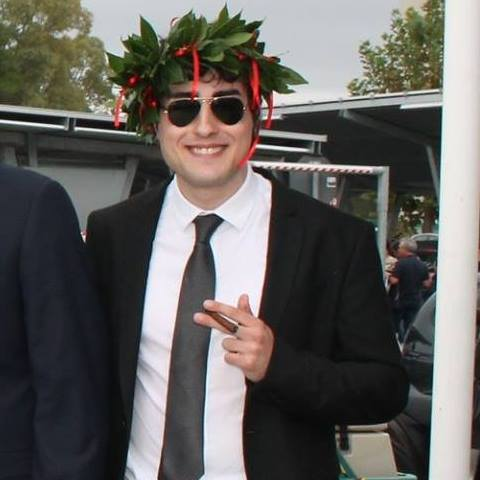
\includegraphics[width=3cm]{figures/marco.jpg}
\vspace{0.3cm}

\raisebox{-0.35ex}{
\includegraphics[width=4ex]{figures/link.png}}%
\hspace{0.05cm} /marcochiarelli

\end{figure}



%BIBLIOGRAFIA - redatta con il relativo ambiente
\begin{thebibliography}{100}
\bibitem{rif1} J. Kurose, K.W. Ross, \emph{Computer Networking. A Top-Down Approach,  sixth edition}
\bibitem{rif2} B.A. Forouzan \emph{Data Communication and Networking, fifth edition}
\bibitem{rif3} P. Oppenheimer \emph{Top Down Networking Design, third edition}
\end{thebibliography}
\end{document}



%************************************************
% Chapter 2: TEORIA DELLE CODE
%************************************************
% !TEX encoding = UTF-8
% !TEX TS-program = pdflatex
% !TEX root = ../nt.tex
% !TEX spellcheck = it-IT

%************************************************
\chapter{TEORIA DELLE CODE}
\label{cap:qtheory}
%************************************************\\

\section{PROCESSI STOCASTICI}

Modello matematico di tipo probabilistico utilizzato per andare a descrivere dei fenomeni casuali che possono essere rappresentati come funzioni di un parametro che solitamente è il tempo. $\{X(t),\ t \in T\}$. Famiglia di variabili casuali $X(t)$, indicizzate dal parametro temporale $t \in T$. Potrebbe anche essere qualche altra grandezza. Le v.a. sono definite su un unico spazio campione e che assumono valori in un certo insieme $S$. I valori assunti sono detti stati. $S$ = spazio degli stati del processo. Un processo stocastico è un insieme di funzioni del tempo. $X(t)$ generica variabile casuale. $X(t)\ \in S$. Insieme di funzioni del tempo che vengono chiamate \textbf{Realizzazioni}. Spazio campione: possibili risultati.

$X(t): T \mapsto S$ SAMPLE PATHS: realizzazioni. La cosa importante è che $X(t)$ è completamente specificato in termini probabilistici se posso scrivere la CDF congiunta (e la PDF). $X(t)$ famiglia di variabili casuali. Differenti realizzazioni. Un processo stocastico è completamente specificato con la CDF congiunta per un qualsiasi insieme (sottoinsieme) di v.a. estratte dal processo. Immaginiamo di estrarre $n$ variabili casuali:

$X(t_i),\ i=1,2,\dots,n$: estrazione di $n$ variabili casuali. Per queste devo essere in grado di scrivere la CDF congiunta:

\[
	F_{\mathbf{\underline{X}}}(\underline{x}; t) := \Pr\{X(t_1) \leq x_1,\ X(t_2) \leq x_2,\ \dots,\ X(t_n) \leq x_n\}
\]

Tale è la CDF CONGIUNTA. Ricordiamo che data una variabile casuale $\xi$, abbiamo che: $F_{\xi}(t) := \Pr\{\xi\leq t\}$. 
Qui bisogna riuscire la scrivere la CDF congiunta per queste $n$ variabili casuali estratte dal processo. In alternativa, potrei considerare la PDF congiunta, la quale è la derivata della CDF. Scriviamo la \textit{ROW VECTOR NOTATION}, generalizzando le casistiche dimensionali:

\[
	\left\{
	\begin{aligned}
	&\mathbf{\underline{X}} = (X(t_1),\ X(t_2),\ \dots,\ X(t_n)) \in\R^{n\times 1}  \\
	&\underline{x} = (x_1,\ x_2,\ \dots,\ x_n) \in\R^{n\times 1}\\
	&\underline{t} = (t_1,\ t_2,\ \dots,\ t_n) \in\R^{n\times 1}
	\end{aligned}
	\right.
\]

Ricordiamo, ancora: $[f_{\mathbf{\underline{X}}}(\underline{x}; t) = \frac{\partial{F_{\mathbf{\underline{X}}}(\underline{x}; t)}}{\partial{\underline{x}}}]$.

\subsection{CATENE DI MARKOV}

Pensiamo allo spazio degli stati $S$. Questo spazio può essere continuo o discreto. Una CATENA è un processo stocastico a stato discreto. Noi tratteremo le \textit{\textbf{CATENE DI MARKOV}}. $t$ può essere continuo o discreto. Tempo continuo o tempo discreto, rispettivamente. Quando il tempo è discreto, si parla di \textit{SEQUENZA STOCASTICA}. Eventualmente potremmo avere: $X_n,\ n=0,1,2,\dots$ ovvero diverse componenti del sistema.

Noi studieremo le CATENE DI MARKOV a tempo continuo, dette \underline{CMTC}. Categoria di processi stocastici. Per questi processi di MARKOV la relazione che intercorre tra le v.a. è molto semplice. Caratterizzazione molto semplice. Questi processi soddisfano la cosiddetta:

\begin{defn}{\textbf{PROPRIET\`A DI MARKOV}}

\[
	\Pr\{X(t) \leq x\ |\ X(t_n) = x_n,\ X(t_{n-1}) = x_{n-1},\ \dots,\ X(t_0) = x_0\} = \Pr\{X(t) \leq x\ |\ X(t_n) = x_n\}
\]

con $t > t_n > t_{n-1} >\ \dots\ > t_0$. 
\end{defn}

Questo è un processo stocastico $\{X(t),\ t\in T\}$ che soddisfa alla proprietà di MARKOV. Si tratta di una CDF condizionata. Cosa mi dice? L'evoluzione futura del processo a partire dall'istante $t_n$ non dipende dalla storia passata ma solo dallo stato finale del processo! L'evoluzione del processo da $t_n$ in poi dipende soltanto da $t_n$. Lo stato in $t_n$ riassume tutta la storia passata del processo. $\{X(t),\ t\in T\}$. Noi studieremo le catene di Markov a tempo continuo (stato discreto, tempo continuo). 

\begin{defn}{\textbf{CM omogenea}}

Invariante rispetto a traslazioni temporali degli assi:

\[
	\Pr\{X(t) \leq x\ |\ x(t_n) = x_n\} = \Pr\{X(t-t_n) \leq x\ |\ X(0) = x_n\}
\]

con $t > t_n$.
\end{defn}

Sono sostanzialmente delle catene per modellare sistemi il quale comportamento NON dipende dal tempo di osservazione. Scelta possibile dell'arco temporale. \underline{OMOGENEIT\`A}.

\begin{defn}{\textbf{COIMPLICAZIONE DELLA PROPRIET\`A DI MARKOV (\textit{tempo di soggiorno})}}

$W_i,\ i\in S$. Uno stato i qualsiasi della mia catena dev'essere una v.a. priva di memoria. Quando una v.a. casuale soddisfa alla proprietà di assenza di memoria, vale il seguente:

\[
	[\Pr\{W_i > t+\tau\ |\ W_i > t\} = \Pr\{W_i > \tau\}]
\]

Tale è la \textit{MEMORYLESS PROPERTY}.
\end{defn}

Se l'evoluzione futura del processo a partire da $t_n$ non dipende dallo stato passato del processo, non dipenderà neanche dal tempo in cui ci è stato. L'unica distribuzione di v.a. continua che soddisfa alla proprietà di assenza di memoria è la

\begin{defn}{\textbf{ESPONENZIALE NEGATIVA UNILATERA}}

\[
	\left\{
	\begin{aligned}
	&[\underline{f_{W_i}(\tau) = a\e^{-a\tau},\ \tau \geq 0}]\\
	&\left\{
	\begin{aligned}
	&F_{W_i}(\tau) = \Pr\{W_i\leq\tau\} = 1-\e^{-a\tau},\ \tau\geq 0\\
	&F_{W_i}^c(\tau) = \Pr\{W_i\geq\tau\} = \e^{-a\tau},\ \tau\geq 0
	\end{aligned}
	\right.
	\end{aligned}
	\right.
\]

\end{defn}

Unica distribuzione di probabilità che soddisfa l'assenza di memoria. Vedremo in seguito come $a := -q_{ii}$ (velocità totale di uscita dallo stato i). Velocità o equivalentemente tasso di transizione.

Proprietà di assenza di memoria per una v.a. casuale (in particolare comporta conseguenze sul tempo di soggiorno in uno stato $i$ di una CMTC):

\[
	\Pr\{W_i > t+\tau\ |\ W_i > t\} = \Pr\{W_i > \tau\}
\]	
	
Parliamone in generale.

\begin{thrm}
L'unica PDF di una v.a. continua che soddisfa alla proprietà di ASSENZA di MEMORIA è l'ESPONENZIALE NEGATIVA UNILATERA (UEN). 
\end{thrm}

\begin{proof}{\textbf{UEN MEMORYLESS PROPERTY}}
\[
	\Pr\{W_i > t+\tau\ |\ W_i > t\} = \frac{\Pr\{W_i > t+\tau,\ W_i > t\}}{\Pr\{W_i > t\}} =(\dots)
\]

Dobbiamo dimostrare questa proprietà per la UEN: $W_i>t+\tau\supseteq W_i>t \implies$

\[ 	
	(\dots) = \frac{\Pr\{W_i > t+\tau\}}{\Pr\{W_i > t\}} = \frac{\e^{-a(t+\tau)}}{\e^{-at}} = \frac{\e^{-at}\e^{-a\tau}}{\e^{-at}} = \e^{-a\tau} = \underline{\Pr\{W_i > \tau\}}
\]

La parte sottolineata sarebbe quindi la CDF complementare $F_{W_i}^c(\tau)$ della UEN.
\end{proof}

A cosa è uguale il parametro $a$? \`E uguale ad $a = -q_{ii}$, che sarebbe la velocità (totale) di uscita dallo stato $i$, ovvero la velocità totale alla quale il processo cerca di uscire dallo stato $i$. Si scrive, posto $a := -q_{ii}$:

\[
	W_i \sim EXP(-q_{ii}),\ \forall i\in S
\]

Quindi il sistema precedente diventa:

\[
	\left\{
	\begin{aligned}
	&[f_{W_i}(\tau) = -q_{ii}\e^{q_{ii}\tau},\ \tau \geq 0]\\
	&\left\{
	\begin{aligned}
	&F_{W_i}(\tau) = \Pr\{W_i\leq\tau\} = 1-\e^{q_{ii}\tau},\ \tau\geq 0\\
	&F_{W_i}^c(\tau) = \Pr\{W_I\geq\tau\} = \e^{q_{ii}\tau},\ \tau\geq 0
	\end{aligned}
	\right.
	\end{aligned}
	\right.
\]

La proprietà di assenza di memoria per $W_i$ dice che, supponendo che il processo stia soggiornando sullo stato i da $t$ unità di tempo, la probabilità che il processo mi soggiorni ancora per altre $\tau$ unità di tempo è pari alla probabilità che il processo soggiorni per $\tau$ unità di tempo. Posto $\tau$ = RESIDUO, definiamo $\Phi_{i,t}$ come tempo di soggiorno residuo nello stato i da $t$ unità di tempo, ovvero il processo si trova già da $t$ unità di tempo nello stato i! Quindi riscriviamo la MLP.

\begin{corl}

\[
	\Pr\{\Phi_{i,t} > \tau\} = \Pr\{W_i > \tau\}
\]

La distribuzione del tempo di soggiorno residuo in un tempo $t$ (LHS) è pari alla distribuzione del tempo di soggiorno (RHS). 

\[
	\left\{
	\begin{aligned}
	&[(W_i \sim \Phi_{i,t}) \sim EXP(-q_{ii})]\\
	&f_{\Phi_{i,t}}(\tau) = -q_{ii}\e^{q_{ii}\tau},\ \tau\geq 0
	\end{aligned}
	\right.
\]

\end{corl}

Nel tempo discreto la distribuzione che soddisfa la MLP è solo quella geometrica. Noi invece lavoriamo a tempo continuo. MARKOVIANIT\`A: assenza di memoria nel processo markoviano. Tempo di soggiorno residuo e tempo di soggiorno non solo hanno la stessa medesima distribuzione esponenziale (UEN), ma sono distribuite anche con lo stesso parametro $-q_{ii} = a$!

Riscriviamo la proprietà di Markov a tempo continuo! (specializzazione): Stiamo lavorando con \underline{CMTC} o CTMC (Continuos Time Markov Chain):

\[
	\Pr\{X(t_{n+1}) = x_{t_{n+1}}\ |\ X(t_n) = x_n,\ X(t_{n-1}) = x_{n-1},\ X(t_0) = x_0\} =
\]
\[
	= \Pr\{X(t_{n+1}) = x_{t_{n+1}}\ |\ X(t_n) = x_n\}
\]

$\forall x_k \in S,\ t_{n+1} > t_n > t_{n-1} >\ \dots\ > t_0$.

Chiamiamo il secondo membro \underline{probabilità di transizione}: $[\Pr\{X(t_{n+1}) = x_{n+1}\ |\ X(t_n) = x_n\}]$. Supponendo che nel tempo $t_n$ il processo si trovi in $x_n$, essa è la probabilità che al tempo $t_{n+1}$ si trovi allo stato $x_{n+1}$. Ma essa non fornisce informazioni circa quello che potrebbe accadere nel frattempo tra $t_n$ e $t_{n+1}$!

\begin{defn}{\textbf{Probabilità di Transizione da i a j}}
\[
	[\underline{p_{ij}(t,\theta) := \Pr\{X(\theta) = j\ |\ X(t) = i\}}]
\]
\end{defn}

$\forall i,j\in S$, e supponendo naturalmente che $\theta > t$.

Se la CMTC è OMOGENEA, queste probabilità di transizione non dipendono dagli istanti di tempo, ma dalla differenza dei due istanti di tempo $[\tau := \theta-t]$.

\[
	[p_{ij}(t,\theta) := \underline{P_{ij}(\tau)} = \Pr\{X(t+\tau) = j\ |\ \underline{\underline{X(t) = i}}\}]
\]

Supponendo che all'istante di tempo $t$ lo stato sia i, quella è la probabilità che dopo $\tau$ istanti di tempo lo stato sia j. Non ci riferiamo più necessariamente ai singoli istanti di tempo. Vale: $[\sum_{j\in S}{p_{ij}(\tau)} = 1]$. Distribuzione al tempo $t$: intendiamo l'insieme di queste probabilità:

\begin{defn}{\textbf{Distribuzione al tempo t}}

\[
	\pi_i(t) := \Pr\{X(t) = i\}\ \forall i\in S
\]
\end{defn}

Andiamo a considerare tutti gli stati del mio processo. Per il teorema delle probabilità totali questa probabilità la posso scrivere in tal modo:

\[
	\pi_i(t) := \Pr\{X(t) = i\} = \sum_{j\in S}{\Pr\{X(t) = i\ |\ X(0) = j\}\Pr\{X(0) = j\}} = \sum_{j\in S}{\underline{p_{ji}(t)}\underline{\pi_j(0)}}
\]

Quindi questa distribuzione al tempo $t$ la possiamo ottenere come somma di prodotti tra la distribuzione iniziale e la probabilità di transizione da j ad i. Possiamo inoltre, dato $\pi_j(0)$, conoscere qualsiasi CDF congiunta. Per ogni processo particolare posso scriverle facilmente... A tempo continuo le probabilità di transizione dipendono però dal tempo! $(\dots) = \mathord{\cdot}(t)$! Per semplificare la vita, sono state introdotte delle quantità legate a $\underline{p_{ji}(t)}$, generalmente anch'esse dipendenti dal tempo, ma che, nel caso in cui la CMTC sia OMOGENEA, sono invece costanti. Queste quantità sono quindi costanti e sono chiamate TASSI o \textit{VELOCIT\`A DI TRANSIZIONE}. Ciò che NON è costante è invece la probabilità di transizione.

\subsubsection{Tassi di Transizione}

\begin{defn}{\textbf{TASSI (o VELOCIT\`A) di transizione}}

Relazione che lega i tassi di transizione alle probabilità di transizione.
Se la catena è regolare:

\[
	\left\{
	\begin{aligned}
	&\exists q_{ij} := \lim_{\Delta t\to 0}{\frac{p_{ij}(\Delta t)}{\Delta t}},	\forall (i\neq j)\in S\\
	&\exists q_{ii} := \lim_{\Delta t\to 0}{\frac{p_{ii}(\Delta t)-1}{\Delta t}} \leq 0
	\end{aligned}
	\right.
\]

$\forall i,j\ \in S$.
\end{defn}

Si può dimostrare che questi limiti, queste quantità, esistono se la CMTC è REGOLARE, ovvero se:

\begin{defn}{\textbf{CMTC REGOLARE}}

\[
	\forall X(0),\ [\underline{\cardinality{transizioni(\Delta t < +\infty)} < +\infty}]
\]
\end{defn}

Questo deve valere per qualunque stato iniziale. $-q_{ii} \geq 0$. Supponiamo che lo stato del processo in $t$ sia $i$ $\iff X(t) = i$. La probabilità che in un intervallo $\Delta t$ tendente a 0 ($\iff \Delta t \to 0$) vi sia una transizione al di fuori di i è: $[-q_{ii}\Delta  t + o(\Delta t)]$.
Ragioniamo invece su $p_{ii}(\Delta t)$: essa rappresenta la probabilità che lo stato presente sia $i$ e tra $\Delta t$ unità di tempo lo stato sia di nuovo $i$. Tale probabilità non mi dice nulla su tutte le possibili transizioni che ci possono essere tra $t$ e $t+\Delta t$.

$1-p_{ii}(\Delta t),\ \Delta t \to 0$ è la probabilità che dopo $\Delta t$ unità di tempo lo stato NON sia più $i$, partendo da $i$ (prob. che vi sia una transizione). Quando $\Delta t \to 0$, questa probabilità tende alla probabilità di leaving dallo stato $i$. Quindi invertendo la seconda equazione del precedente sistema troviamo che al limite essa è uguale a: $[-q_{ii}\Delta t + o(\Delta t)]$. La probabilità è tanto più grande quando $q_{ii}$ è alto in modulo! Più velocemente esce, più è probabile che esca! Più grande è il valore $\abs{q_{ii}}$, più il processo cerca di uscire velocemente, e quindi con maggior probabilità vi riuscirà $\implies \abs{q_{ii}} \uparrow \implies$ processo più velocemente tende ad uscire.

$-q_{ii}$ è quindi la velocità alla quale un processo lascia lo stato $i$. In sostanza, $-q_{ii}$ rappresenta il numero medio di transizioni al di fuori di $i$ $\forall$ unità di tempo \newline
\underline{in cui il processo si trova nello stato $i$}.

Prendiamo per esempio due diverse realizzazioni dello stesso processo: $\{X^{(1)}(t),\ X^{(2)}(t)\}$. Per $X^{(1)}(t)$ abbiamo diversi soggiorni nello stato i. Supponiamo che la somma delle durate di soggiorno in $i$ facciano $1s$. Durante questa unità di tempo in cui il processo si trova in $i$, si trovano 7 transizioni al di fuori di $i$. Per $X^{(2)}(t)$, supponiamo lo stesso caso ma con 5 transizioni. Abbiamo detto che: $-q_{ii}$ è il numero medio di transizioni al di fuori dello stato $i$. Una transizione uscente segue un \underline{tempo di soggiorno}. $-q_{ii}$ rappresenta quindi anche il tempo medio di soggiorno. Ricordando che $f_{W_i}(\tau) = -q_{ii}\e^{q_{ii}\tau}$, abbiamo che:

\[
	\E[W_i] = \frac{1}{-q_{ii}}
\]

Se calcoliamo il valor medio (la media) di $f_{W_i}(\tau)$, esce proprio $(\frac{1}{-q_{ii}})$; tanto più grande è $q_{ii}$, tanto basso sarà il tempo di soggiorno in media.

Significato di $q_{ij}$. Supponiamo che attualmente il processo si trovi in $i$. La probabilità che in un intervallo di tempo infinitesimo ($\Delta t \to 0$) vi sia una transizione $ij$, ($i \rightarrow j$), è uguale alla probabilità $q_{ij}\Delta t + o(\Delta t)$. Consideriamo $p_{ij}(t)$. Non mi dice nulla, essendo una probabilità di transizione, su cosa sia eventualmente accaduto nel rispettivo intervallo di tempo tra la transizione.

Accade quindi che:

\[
	[\lim_{\Delta t \to 0}{\frac{p_{ij}(t)}{\Delta t}} = q_{ij}]
\]

(probabilità tanto più grande quanto più grande è $q_{ij}$).
La velocità è $q_{ij}$. Rappresenta una velocità alla quale si verifica la transizione $i \rightarrow j$. Ecco perché viene detto TASSO (o VELOCIT\`A) di TRANSIZIONE da $i$ a $j$. Ma è anche in sostanza il numero medio di transizioni da $i$ a $j$ $(i \rightarrow j) \ \forall$ unità di tempo in cui il processo si trova nello stato i$i$ Ragioniamo di nuovo sulle due funzioni rappresentanti due diverse realizzazioni dello stesso processo. Supponiamo sempre che la durata complessiva di un soggiorno in $i$ sommi temporalmente ad 1. $q_{ij}$ si differenzia da $-q_{ii}$ in quanto rappresenta il numero medio di transizioni ($i \rightarrow j$).

\[
	\sum_{(j\neq i)\in S}{q_{ij}} = \sum_{(j\neq i)\in S}{(\lim_{\Delta t \to 0}{\frac{p_{ij}(\Delta t)}{\Delta t}})} = \lim_{\Delta t \to 0}{\sum_{(j\neq i)\in S}{(\frac{p_{ij}(\Delta t)}{\Delta t})}} = (\dots)
\]

Considerando uno stato $i$ qualsiasi, questa sommatoria fa 1: $\iff \sum_{j\in S}{p_{ij}(\Delta t)} = 1$. Quindi:

\[
	(\dots) = \lim_{\Delta t \to 0}{\frac{1-p_{ii}(\Delta t)}{\Delta t}} = \underline{\underline{-q_{ii}}}
\]

La quale è la velocità \underline{totale} di uscita dallo stato $i$. Introduciamo ora una seconda quantità: $[\tau_{i,j} = \frac{q_{ij}}{-q_{ii}}]$, ovvero la probabilità che il processo, lasciando lo stato i, faccia una transizione verso lo stato $j$. 

Supponiamo che $q_{ij}=10,\ q_{ik}=30,\ q_{ih}=60$... mediamente vi siano quindi 100 transizioni uscenti. $-q_{ii} = \sum_{(j\neq i)\in S}{q_{ij}} = 100$. Abbiamo che:

\[
	\left\{
	\begin{aligned}
	&\tau_{i,j} = \frac{10}{100} = 0.1\\
	&\tau_{i,h} = \frac{60}{100} = 0.6\\
	&\tau_{i,k} = \frac{30}{100} = 0.3
	\end{aligned}
	\right.
\] 

$\tau_{i,j}$ è quindi alla fine la probabilità che, supponendo di lasciare $i$, la transizione sia verso $j$. LASCIANDO LO STATO $i$, $\exists$ UNA TRANSIZIONE VERSO LO STATO $j$.

Distribuzione al tempo $t$. Ci sono dei sistemi di equazioni differenziali che legano la distribuzione al tempo $t$ ai tassi di transizione:

\[	
	\left\{
	\begin{aligned}
	&\underline{\pi_i}(t) := \Pr\{X(t) = i\},\ \forall i\in S\\
	&\frac{d \pi_i(t)}{dt} = \sum_{j\in S}{q_{ji}\pi_j(t)},\ \forall i\in S
	\end{aligned}
	\right.
\]

Di queste equazioni differenziali ve n'è una $\forall s\in S$ della nostra catena. Nella maggior parte dei casi, non ci serve $\pi_i(t)$, ma una distribuzione a regime (costante). A regime serve la rispettiva distribuzione a regime (dopo un tempo molto grande). Ci sono delle condizioni in base alla quale $\pi_i(t) \to K \neq \mathord{\cdot}(t)$ (distribuzione di equilibrio, a regime). Ma quali sono queste condizioni?

\subsection{Probabilità a regime}

Quali sono le condizioni di esistenza delle probabilità di stato a regime? Introduciamo alcune definizioni. Consideriamo uno stato $i \in S$ della mia \underline{CMTC}. Diciamo che lo stato $(i\in S)$ è \textit{TRANSITORIO} se c'è una probabilità non nulla che il processo non torni più in quello stato dopo che esso viene lasciato. Si dirà \textit{RICORRENTE} in caso contrario (se con probabilità 1 torni nello stato $i$ dopo averlo lasciato). Ai fini della distribuzione di regime, a noi interessano i RICORRENTI (gli stati ricorrenti). Sia $M_i$ il tempo medio di ritorno (o \underline{di ricorrenza} nello stato $i$). Per tempo di ritorno si intende il tempo che passa da \underline{due ingressi consecutivi} nello stato $i$. $M_i$ dice quanto dura in media questo tempo (ovviamente guardando tutte le possibili realizzazioni, altrimenti sarebbe costante). Si consideri una finestra temporale ($M_i$), è contemplato in media un solo soggiorno in $i$! (UN SOLO tempo di soggiorno). Se questo valore diverge ($\iff M_i \to +\infty$), lo stato è detto \textit{RICORRENTE NULLO}. Se $M_i$ converge parliamo di STATO \textit{RICORRENTE NON NULLO}.

Consideriamo ora un sottoinsieme proprio dello spazio degli stati $A\subset S\ |\ \bar{A} \cup A = S$. $A$ comprende una parte degli stati, e non può coincidere con $S \iff \bar{A} = S \setminus (A\neq \emptyset)$.

Vale:

\begin{thrm}
$A$ chiuso se:

\[
	\sum_{i\in A}{\sum_{j\in\bar{A}}{q_{ij}}} = 0
\]
\end{thrm}

Significa che una volta che il processo entra in $A$, NON esce da $A$! In particolare, chiamiamo \textit{STATO TRAPPOLA} od \textit{ASSORBENTE} uno stato $i$ per il quale: $ [q_{ii} = -q_{ii} = 0]$ (Il processo NON esce più da quello stato). Uno STATO TRAPPOLA corrisponde ad un insieme chiuso costituito da solo quello stato.

\begin{defn}{\textbf{CM IRRIDUCIBILE}}

Una CTMC è \underline{\underline{IRRIDUCIBILE}} se $\nexists$ insiemi chiusi $\iff$ Tutti gli stati COMUNICANO tra di loro. Da $i$ a $j$ ci arrivo (magari passando da altri stati), ma ci arrivo sempre prima o poi! $i \leftarrow\rightarrow j\ \forall i,j\in S$.

\end{defn}

Abbiamo quindi tre caratterizzazioni di stato: (tre diversi possibili tipi di stato):

\begin{itemize}

\item{\textit{TRANSITORI}};
\item{\textit{RICORRENTI NULLI}};
\item{\textit{RICORRENTI NON NULLI}}.

\end{itemize}

\begin{corl}{\textbf{Omogeneità dei tipi di stato per CM IRRIDUCIBILE}}

Qualora una CM sia IRRIDUCIBILE $\implies$ allora tutti gli stati sono dello stesso tipo.

\end{corl}

Concetto molto forte. CATENA IRRIDUCIBILE $\iff$ tutti gli stati comunicano $\iff$ tutti gli stati sono dello stesso tipo. Ricordiamo:

\[
	[\frac{d \pi_i(t)}{dt} = \sum_{j\in S}{q_{ji}\pi_j(t)}]
\]

\begin{defn}{\textbf{PROBABILIT\`A LIMITE}}
\[
	[\pi_i := \lim_{t\to\infty}{\pi_i(t)}]
\]
$\forall i\in S$.
\end{defn}

Se una CATENA è OMOGENEA, IRRIDUCIBILE (Quando una CATENA è OMOGENEA i tassi di transizione sono COSTANTI), allora:

\[
	\exists \lim_{t\to\infty}{\pi_i(t)} := \pi_i \neq \mathord{\cdot} \pi_i(0)
\]

Se vogliamo avere delle distribuzioni a regime, vogliamo che questa quantità esista finita (limite esistente e convergente). In particolare non devono dipendere dalle probabilità di \underline{stato iniziali}. In tal caso il sistema di equazioni differenziali collassa in un sistema di equazioni algebriche lineari:

\[
	[\sum_{j\in S}{q_{ji}\pi_j} = 0]
\]

$\forall i\in S$. Le derivate vanno quindi a 0 $\iff \pi_i(t) \tendsto{t\to\infty} \pi_i$. Questo sistema è OMOGENEO (sicuramente comprende la soluzione nulla). Tante soluzioni quanti sono gli stati del processo. SE la soluzione nulla fosse l'unica soluzione, gli stati saranno tutti TRANSITORI o tutti RICORRENTI nulli e non avremmo quindi una distribuzione di regime ($\iff \nexists \pi_i$). Se così non fosse invece, in tal caso le soluzioni saranno un numero infinito, che differirranno per una \underline{costante moltiplicativa} tra di loro. Se sono infinite (tutte linearmente dipendenti), tra tutte queste le filtriamo con la cosiddetta condizione di normalizzazione. In tal caso gli stati saranno tutti \underline{RICORRENTI NON NULLI}.

\begin{defn}{\textbf{ERGODICIT\`A}}

\[
	\left\{
	\begin{aligned}
	&\sum_{j\in S}{q_{ji}\pi_j} = 0,\ \forall i\in S\\
	&\sum_{i\in S}{\pi_i} = 1
	\end{aligned}
	\right.
\]

$\exists SOL$? Se esiste, in tal caso la CATENA è detta \textit{ERGODICA} (proprietà di ERGODICIT\`A). \underline{CMTC} \{OMOGENEA, IRRIDUCIBILE, (STATI RICORRENTI NON NULLI)\}.\end{defn}

Innanzitutto, si verifichi l'OMOGENEIT\`A guardando i tassi di transizione (diagrammi di stato). Devono essere costanti (OMOGENEA, \underline{\underline{IRRIDUCIBILE}} (stati dello stesso tipo)). Basterebbe, per verificare che gli stati siano TUTTI ricorrenti non nulli, verificare questa proprietà per UN SOLO STATO! Ma a questo punto, senza ragionare su $M_i$, ragiono sull'equazione e la risolvo, sperando di risolverla e di trovare UNA ed UNA SOLA soluzione.

\begin{corl}{\textbf{Caratterizzazione dell'Ergodicita'}}

Se abbiamo una [CMTC OMOGENEA, IRRIDUCIBILE e con un numero di stati finito $(\iff\cardinality{stati}<+\infty)$], sicuramente essa è \underline{ERGODICA}].

\end{corl}

Abbiamo detto che $\pi_i,\ i\in S$ sono le probabilità limite, QUANTIT\`A valutate IN VERTICALE, ed hanno a che fare con le distribuzioni di regime. MA è anche la frazione di tempo a regime in cui lo stato sia $i$.

\subsection{ERGODICIT\`A}

Condizioni di ERGODICIT\`A per una CMTC: \{OMOGENEA, IRRIDUCIBILE, con STATI RICORRENTI NON NULLI\} $\implies [\exists \lim_{t\to\infty}{\pi_i(t)} := \pi_i]$. Una volta veriifcate queste due proprietà, non c'è bisogno di verificare che gli stati siano tutti RICORRENTI NON NULLI. In maniera più semplice si tenta di risolvere quel sistema sperando che abbia una soluzione non banale. Diagramma dei tassi di transizione: \{Cerchi = Stati, Archi = Transizioni, pesate con i tassi di transizione\}. Se questi tassi non sono dipendenti dal tempo allora la catena è OMOGENEA. 

\[
	[\underline{\pi_i} = \lim_{t\to\infty}{(\pi_i(t) = \Pr\{X(t)=i\})},\ \forall i\in S
\]

La distribuzione di regime ha ovviamente a che fare con le probabilità limite. Immaginiamo che la catena sia ERGODICA. $\pi_i$ = probabilità che a regime lo stato sia $i$. Se la catena è \underline{ergodica}, allora a $\pi_i$ possiamo attribuire un altro significato: frazione del tempo (A REGIME) in cui lo stato sia $i$:

\[
	[\pi_i = \lim_{t\to\infty}{\frac{T_i(t)}{t}}]
\]

dove $T_i(t)$ è il tempo trascorso dal processo \underline{nello stato $i$} sino al tempo $t$. (SINGOLA REALIZZAZIONE). \`E come se stessimo guardando una singola realizzazione del processo. Presa una finestra $[0,t) \leftarrow T_i(t)$. Fino al tempo $t$. Se calcolo $\frac{T_i(t)}{t}$, allora ottengo la frazione di tempo nel quale il processo è stato nello stato $i$ nell'intervallo di tempo definito dalla finestra temporale scelta.

es. $\pi_i = 0.2 \implies$ per il 20\% il processo a regime si è trovato in $i$. $\pi_i\tau$ rappresenta il tempo in media nel quale il processo si è trovato nello stato $i$ durante la finestra temporale di durata $\tau$. $\pi_i$ è da valutare sull'INSIEME delle realizzazioni.

Consideriamo $N(t)$ processo stocastico che rappresenta il numero di clienti (\#) in un sistema a coda. Esaminiamo un certo numero di realizzazioni.

Dal momento che $\pi_i(t)$ è una probabilità, essa va valutata in verticale. Supponiamo che:

\[
	\left\{
	\begin{aligned}
	&n_R := \cardinality{realizzazioni\ di\ N(t)}\\
	&n_i(t) := n_i = \cardinality{realizzazioni\ con\ stato\ i\ nell'istante\ t}
	\end{aligned}
	\right.
\]

$(\frac{n_i}{n_R})$ rappresenta la frazione delle $n_R$ realizzazioni con stato pari ad $i$ in $t$. Quando $n_R$ cresce, $\iff n_R \uparrow ,\ (\frac{n_i}{n_R}) \tendsto{}$ probabilità che lo stato del processo sia $i$.

Rispettivamente:

\begin{thrm}{\textbf{Probabilità Limite}}

\[
	\lim_{n_R\to\infty}{(\frac{n_i}{n_R})} = \pi_i(t) = \Pr\{X(t)=i\}
\]
\end{thrm}

Tutto questo a regime! Abbiamo considerato $\pi_i$ valutandola con un numero molto grande di realizzazioni. Guardando invece ad una singola realizzazione di tempo molto grande ($\iff t\to +\infty$), abbiamo che: $\underline{\pi_i} = \lim_{t\to\infty}{\frac{T_i(t)}{t}}$, che sarebbe la frazione in cui il processo si è trovato in $i$ nella finestra temporale $[0,t)$.

\begin{thrm}{\textbf{Mapping VERTICALE ORIZZONTALE}}

Se c'è l'ERGODICIT\`A abbiamo che:

\[
	\underline{\pi_i} = \lim_{n_R\to\infty}{(\frac{n_i}{n_R})} = \pi_i(t) = \Pr\{X(t)=i\} = \lim_{t\to\infty}{\frac{T_i(t)}{t}}
\]
\end{thrm}

Si consideri ora: $\bar{N} = \sum_{i=0}^\infty{i\pi_i}$. Questo è la media del numero di clienti. Numero medio di clienti del sistema a regime (si noti l'estremo superiore della sommatoria). Ma se il processo è ERGODICO, la media di insieme coincide con la media temporale. Nella pratica si suppone l'\underline{ergodicità}, si procede in orizzontale. Si consideri $\lim_{t\to\infty}{\bar{N_t}}$. Senza il limite essa rappresenta il valore medio assunto da quelle funzioni: $\bar{N_t} := \frac{1}{t}\int_0^t{N(\tau)d\tau}$ (MEDIA TEMPORALE) durante la finestra temporale $[0,t)$. Se c'è l'ERGODICIT\`A allora questa quantità, AL LIMITE di $t\to\infty$ coincide con $\bar{N} \iff [\lim_{t\to\infty}{\bar{N_t}} = \bar{N}]$ = VALORE DI REGIME.

\subsubsection{ERGODICIT\`A (RECAP)}

$\{\pi_i,\ \pi_i\tau\}$ rappresentano rispettivamente la probabilità che \underline{a regime} il processo si trovi in $i$, ed il tempo medio che il processo si trova in $i$ nella finestra temporale di lunghezza $\tau$. $M_i$ = tempo medio di ritorno nello stato $i$. Supponiamo di avere $\tau = M_i$. Sarebbe il tempo tra due ingressi consecutivi nello stato $i$ = tempo di ricorrenza. VALOR MEDIO $M_i$. \`E necessariamente un tempo di soggiorno. Quindi: 

$\pi_iM_i$ = tempo medio trascorso nello stato $i$ durante la finestra temporale $\tau = M_i$. Ma abbiamo \underline{un solo soggiorno} durante $M_i \iff [\underline{\pi_iM_i} = \E[W_i] = \frac{1}{-q_{ii}}]$. Invertendo troviamo: $M_i = \frac{1}{-q_{ii}\pi_i}$ (tempo medio di ricorrenza). Ricordiamo che:

\[
	\underline{f}_{W_i}(\tau) = -q_{ii}\e^{q_{ii}\tau},\ \tau\geq 0
\]

Ed avendo un solo soggiorno $\underline{\pi_iM_i}$ rappresenta il TEMPO \underline{MEDIO DI SOGGIORNO}. Possiamo dare una formulazione matriciale dell'insieme di equazioni differenziali:

\[
	\left\{
	\begin{aligned}
	&\frac{d \pi_i(t)}{dt} = \sum_{j\in S}{q_{ji}\pi_j(t)},\ \forall i\in S\\
	&\frac{d \underline{\pi(t)}}{dt} = \underline{\pi(t)}\underline{Q}
	\end{aligned}
	\right.
\]

$\underline{\pi}$ è il vettore riga delle probabilità di stato al tempo t, indicizzato da $i$. Nel caso di ERGODICIT\`A ovviamente vale che: $[\underline{\pi}\underline{Q} = \underline{0}]$ (vettore nullo).

\subsection{CMTC Nascita e Morte}

Caso particolare di CMTC, utili per lo studio dei sistemi a coda. CATENE DI NASCITA E MORTE per una CMTC. Caso particolare di CMTC. Sono dette così perché si prestano bene a modellare una evoluzione, dinamica di una popolazione (dimensione della popolazione). Abbiamo incrementi o decrementi di stato UNITARI $\iff\ \{i++,\ i--\}$. Ci interessano molto. Sono delle catene definite sullo spazio degli stati $S = \{0,1,2,\ \dots\}$. Tale spazio può essere di dimensione illimitata. Ma tipicamente lo spazio per noi sarà tale che $\cardinality{S} < +\infty$. Catene caratterizzate da fatto che vi sono incrementi/decrementi solo unitari.

Sia $N(t) = i$, quello che può accadere è che: $\{N(t) = i \to i+1\ \lor\ N(t) = i \to i-1\}$. Nel DTT (diagramma dei tassi di transizione), gli archi ricordiamo che rappresentano delle transizioni, e sono pesati dai tassi (o velocità) di transizione. DTT sarà fatta con cerchi che rappresentano gli stati, e gli archi rappresentanti le transizioni, pesati con i rispettivi tassi (o velocità).

\begin{center}
\begin{tikzpicture}[->, >=stealth', auto, semithick, node distance=1.9cm]
\tikzstyle{every state}=[fill=white,draw=black,thick,text=black,scale=1]
\node[state]    (0)                     {$0$};
\node[state]    (1)[right of=0]   {$1$};
\node[state]    (2)[right of=1]   {$2$};
\node[state] (d) [right of=2] {\ldots};
\node[state]    (im1)[right of=d]   {$i-1$};
\node[state]    (i)[right of=im1]   {$i$};
\node[state]    (ip1)[right of=i]   {$i+1$};
\node[state]    (d2)[right of=ip1]  {\ldots};
\path
(0) edge[bend left]     node{$\lambda_0$}         (1)
(1) edge[bend left]     node{$\lambda_1$}         (2)
    edge[bend left,below]    node{$\mu_1$}            (0)
(2) edge[bend left]     node{$\lambda_2$}           (d)
    edge[bend left,below]    node{$\mu_2$}             (1)
(d) edge[bend left]         node{$\lambda_{i-2}$}   (im1)
	edge[bend left,below]   node{$\mu_3$}          (2)
(im1) edge[bend left]       node{$\lambda_{i-1}$}  (i)
	  edge[bend left,below]   node{$\mu_{i-1}$}     (d)
(i)   edge[bend left]   node{$\lambda_i$}      (ip1)
      edge[bend left,below]  node{$\mu_i$}          (im1)
(ip1) edge[bend left]       node{$\lambda_{i+1}$}  (d2)
	 edge[bend left,below]   node{$\mu_{i+1}$}      (i)
(d2) edge[bend left,below]   node{$\mu_{i+2}$}     (ip1);
\end{tikzpicture}
\end{center}

Tipicamente in un DTT per una catena di questo tipo abbiamo che sopra ci sono le nascite ($\lambda_i$), e sotto vi sono le morti ($\mu_i$). Rispettivamente:

\begin{defn}{\textbf{Tassi di nascita e morte}}

\[
	\left\{
	\begin{aligned}
	&\lambda_i :=\ tasso\ di\ nascita\ sullo\ stato\ i\\
	&\mu_i :=\ tasso\ di\ morte\ nello\ stato\ i
	\end{aligned}
	\right.
\]
\end{defn}

Se questi valori sono COSTANTI $\iff$ la CATENA è OMOGENEA. Se la catena è IRRIDUCIBILE: tutti gli stati comunicano $\implies [\exists\pi_i = \lim_{t\to\infty}{\pi_i(t)}]\ \forall i\in S$. Il numero di stati però NON è finito! $(\iff \cardinality{S} = +\infty)$. Quindi dobbiamo cercare di risolvere il sistema:

\[
	\left\{
	\begin{aligned}
	&\sum_{j=0}^\infty{q_{ji}\pi_j} = 0\\
	&\sum_{i=0}^\infty{\pi_i} = 1\ (CONDIZIONE\ DI\ NORMALIZZAZIONE)
	\end{aligned}
	\right.
\]

Abbiamo che: $-q_{00} = \lambda_0$ (velocità totale di uscita dallo stato 0). Quindi: $-\lambda_0\pi_0 + \mu_1\pi_1 = 0$ per lo stato 0, poi dato che vale: $-q_{11}=\lambda_1 + \mu_1$, allora per lo stato 1: $\lambda_0\pi_0 -( \lambda_1+\mu_1)\pi_1 + \mu_2\pi_2 = 0$. Genericamente allo stato i abbiamo:

\[
	"i" \rightarrow\ \lambda_{i-1}\pi_{i-1} - (\lambda_i +\mu_i)\pi_i + \mu_{i+1}\pi_{i+1} = 0
\]

Queste si chiamano EQ. DI BILANCIAMENTO TOTALE. Noi scriviamo le equazioni in generale per una \underline{CMTC ERGODICA}. $\sum_{j\in S}{q_{ji}\pi_j} = 0\ \forall i\in S$. Proviamo a tirare fuori il termine della sommatoria per $j=i$:

\[
	\implies \sum_{(j\neq i)\in S}{q_{ji}{\pi_j}} = -q_{ii}\pi_i
\]

Generalizzando possiamo scrivere le:


\begin{thrm}{\textbf{EQUAZIONI DI BILANCIAMENTO TOTALE}}

\[
	\sum_{(j\neq i)\in S}{q_{ji}\pi_j} = \sum_{(j\neq i)\in S}{q_{ij}\pi_i}
\]

\end{thrm}

Esse esprimono il fatto che a regime (od equilibrio), la frequenza delle transizioni entranti nello stato $i$ eguaglia la frequenza delle transizioni uscenti dallo stato $i$. \`E sostanzialmente un altro modo di scrivere: $\sum_{j\in S}{q_{ji}\pi_j} = 0\ \forall i\in S$. Il numero medio (per unità di tempo) di transizioni entranti nello stato $i$ è uguale al numero medio di transizioni uscenti nello stato $i$. $q_{ji}\pi_j$ è la frequenza (quindi adimensionale) delle transizioni dallo stato $j$ allo stato $i$. Numero medio di transizioni nello stato $i$ (per unità di tempo).

$q_{ji}$ = numero medio di transizioni da $j$ ad $i\ \forall$ unità di tempo in cui il processo si trova nello stato $j$, mentre $\pi_j$ è una frazione di tempo. Ricordiamo che scelta ad esempio una finestra temporale $\tau=1s$, allora il prodotto $\pi_j\tau$ rappresenta il tempo medio trascorso durante questa finestra temporale ($\tau=1s$) dal processo nello stato $j$. Se facciamo $q_{ji}\pi_j$ otteniamo invece il numero medio di transizioni da $j$ ad $i$ $\forall$ unità di tempo. 

L'intera equazione dice che all'equilibrio la frequenza delle transizioni verso lo stato $i$ è pari alla frequenza di transizioni uscenti dallo stato $i$. All'equilibro il flusso entrante nello stato $i$ è pari al suo flusso uscente. Si eguaglia praticamente ($\forall$ stato), flusso entrante (IN) e flusso uscente (OUT). Quindi dobbiamo bilanciare il flusso caso per caso.

Consideriamo l'equazione di bilanciamento per il generico stato $i$:

\[	
	(\lambda_{i-1}\pi_{i-1} + \mu_{i+1}\pi_{i+1} = IN) = ((\lambda_i +\mu_i) = OUT)
\]

Per lo stato 0 abbiamo: $\mu_1\pi_1 = \lambda_0\pi_0$.
Vale per qualunque CMTC \underline{ERGODICA}.

\begin{thrm}{\textbf{EQUAZIONI DI BILANCIAMENTO TOTALE generalizzate}}

Possiamo considerare $(A \subset S) \supset \{statuses\}$. Si immagini di considerare come macrostati gli insiemi di stato $\{0,\ \dots,\ i\}$. Valgono le eq. di bilanciamento totale generalizzate: Flusso uscente da A = flusso entrante in A:

\[
	\sum_{j\in \bar{A},i\in A}{q_{ij}\pi_i} = \sum_{j\in \bar{A},i\in A}{q_{ji}\pi_j}
\]

\end{thrm}

Inoltre, ne deriva che per una BDCMTC abbiamo di conseguenza:

\begin{corl}{\textbf{EQUAZIONI DI BILANCIAMENTO TOTALE GEN. per BD-CMTC}}

\[
	[(\lambda_i\pi_i)_{OUT} = (\mu_{i+1}\pi_{i+1})_{IN}]
\]

\end{corl}

Tentiamo ora di eguagliare il flusso sulla frontiera verticale tra due stati. Otteniamo:

\begin{thrm}{\textbf{EQUAZIONI DI BILANCIAMENTO LOCALE}}


\[
	\pi_iq_{ij} = \pi_jq_{ji}
\]

\end{thrm}

QUESTE valgono soltanto IN CASI PARTICOLARI (BDCMTC). Le GLOBALI e quelle GLOBALI GENERALIZZATE valgono invece SEMPRE per una CMTC.

Si considerino queste equazioni trovate per una BDCMTC:

\[
	\left\{
	\begin{aligned}
	&\lambda_i\pi_i = \mu_{i+1}\pi_{i+1},\ i\geq 0\\
	&\sum_{i=0}^\infty{\pi_i} = 1\ as\ C.N.
	\end{aligned}
	\right.
\]

Quindi abbiamo: $\pi_{i+1} = \frac{\lambda_i \pi_i}{\mu_{i+1}}$. Prendiamo $(i=0) \implies \pi_1 = \pi_0 \frac{\lambda_0}{\mu_1}$. Andando avanti ricorsivamente troviamo:

\[
	\left\{ 
	\begin{aligned}
	&i=1 \implies \pi_2 = \pi_1 \frac{\lambda_1}{\mu_2} = (\pi_0 \frac{\lambda_0}{\mu_1})\frac{\lambda_1}{\mu_2}\\
&i=2 \implies \pi_3 = \pi_2 \frac{\lambda_2}{\mu_3} = (\dots) = \pi_0 \frac{\lambda_0\lambda_1\lambda_2}{\mu_1\mu_2\mu_3}\\
&i-1 \implies \underline{\pi_i} = \pi_0 \frac{\lambda_0\lambda_1\lambda_2\dots\lambda_{i-1}}{\mu_1\mu_2\dots\mu_i} = \pi_0\prod_{k=0}^{i-1}{\frac{\lambda_k}{\mu_{k+1}}},\ i \geq 1
	\end{aligned}
	\right.
\]

Abbiamo quindi trovato le espressioni per le:

\begin{defn}{\textbf{Probabilità a regime}}

\[
	[\underline{\pi_i} = \pi_j\prod_{k=j}^{i-1}{\frac{\lambda_k}{\mu_{k+1}}}] = \mathord{\cdot}(\pi_j)
\]
\end{defn}

Adesso vogliamo mettere in gioco la condizione di normalizzazione: Quindi essa diventa:

\[
	[\pi_0 + \sum_{i=1}^{\infty}{\pi_i} = 1] \implies \pi_0 + \sum_{i=1}^{\infty}{\pi_0\prod_{k=0}^{i-1}{\frac{\lambda_k}{\mu_{k+1}}}} = 1 = \pi_0(1 + \sum_{i=1}^{\infty}{\prod_{k=0}^{i-1}{(\frac{\lambda_k}{\mu_{k+1}})}}) = 1 \implies
\]
\[
	\pi_0 = \frac{1}{1 + \sum_{i=1}^{\infty}{\prod_{k=0}^{i-1}{(\frac{\lambda_k}{\mu_{k+1}})}}}
\]

with:

\[
	\pi_i = [\pi_0 \prod_{k=0}^{i-1}{\frac{\lambda_k}{\mu_{k+1}}}],\ i \geq 1
\]

\begin{corl}

Se la sommatoria a denominatore di $\pi_0$ converge, allora la soluzione esiste. Quindi:

\[
	\pi_i = [\frac{1}{1 + \sum_{i=1}^{\infty}{\prod_{k=0}^{i-1}{(\frac{\lambda_k}{\mu_{k+1}})}}}] \prod_{k=0}^{i-1}{\frac{\lambda_k}{\mu_{k+1}}},	 i \geq 1
\]
\end{corl}

\newpage

\subsection{PROCESSO DI POISSON}

\`E un caso particolare di BDCMTC nel quale i tassi di nascita sono costanti e pari a $\lambda_i = \lambda \neq \mathord{\cdot}(i)\ \land\ \mu_i = 0\ \forall i\in S$. \`E sottinteso che il processo sia omogeneo. Il processo è di pura nascita. Lo spazio degli stati è il seguente: $S = \{0,1,2,\ \dots\}$. Tutti gli stati sono TRANSITORI (una volta uscito da uno stato NON vi ritorno più) $\implies \nexists (\pi_i \neq \mathord{\cdot}(t))$. 

\[
	\left\{
	\begin{aligned}
	&\frac{d \pi_i(t)}{dt} = \sum_{j\in S}{q_{ji}\pi_j(t)},\ \forall i\in S\\
	&\underline{\underline{\pi_0(0)}} = 1
	\end{aligned}
	\right.
\]

dove l'ultima equazione del sistema rappresenta la condizione iniziale, sempre da rispettare. Per un processo di POISSON abbiamo che la distribuzione soddisfa alla seguente:

\begin{defn}{\textbf{Funzione massa di probabilità per un Processo di POSSION}}

\[
	\pi_i(t) = \Pr\{X(t) = i\} = \frac{(\lambda t)^i}{i!}\e^{-\lambda t},\ t\geq 0,\ \forall i\in S
\]

\end{defn}

Questa espressione mi ricorda la distribuzione di POISSON con parametro $(a := \lambda t)$. Avendo una v.a. distribuita con Poisson con parametro $a \implies a = \E[X]$. Disegnamo una possibile realizzazione del processo. Supposto che evolva a partire dallo stato 0. Abbiamo:

$\{\tau_1 = W_1,\ \tau_2 = W2,\ \dots,\ \tau_n = t_n-t_{n-1}\}$. Possiamo quindi scrivere la PDF del tempo di soggiorno negli stati:

\[
	[f_{\tau_n}(r) = \lambda\e^{-\lambda r},\ r \geq 0]
\]

ove (\underline{$\tau_n$ = tempo di soggiorno negli stati}). Queste variabili casuali sono distribuite secondo Poisson. Il processo di POISSON modella gli arrivi dei pacchetti alle code dei router. Arrivi dei clienti in un sistema a coda. Supponiamo di utilizzare al posto di $X(t)$, $A(t)$. \textit{ARRIVAL}. Posso dire che questo processo CONTEGGIA gli arrivi sino a $t$. PROCESSO DI CONTEGGIO DEGLI ARRIVI sino a $t$. $\tau$ sono tempi di INTER-ARRIVO (quanto tempo è passato tra l'arrivo del cliente (n-1)-esimo e quello n-esimo) $\iff [\tau_n = t_n - t_{n-1}]$ sono i tempi di inter-arrivo tra i clienti. SE STO UTILIZZANDO UN PROCESSO DI POISSON per modellare GLI ARRIVI, allora abbiamo che il tempo di soggiorno è sempre distribuito esponenzialmente in maniera negativa unilatera. 

\begin{corl}{\textbf{Omogeneità del Processo di POISSON}}

\[
	\left\{
	\begin{aligned}
	&\Pr\{A(t) = i\} = \frac{(\lambda t)^i}{i!}\e^{-\lambda t}\\
	&\Pr\{A(t)-A(s<t) = i\} = \frac{(\lambda \tau)^i}{i!}\e^{-\lambda \tau}
	\end{aligned}
	\right.
\]

con $\tau := t-s$. 

\end{corl}

Il precedente corollario vale GRAZIE AL FATTO CHE LA CATENA \`E OMOGENEA. 

\subsubsection{RECAP}

Processo di Poisson, caso particolare di una CMTC di nascita e morte (BDCMTC). Tipicamente utilizzato per modellare i clienti in ARRIVO ad un sistema a coda. In questo caso lo possiamo vedere come un processo di conteggio degli arrivi. I tempi di interarrivo sono v.a. indipendenti identicamente distribuite con distribuzione esponenziale negativa unilatera. Rispettivamente, le variabili casuali $[\tau_n = t_n-t_{n-1}]$ avranno questa PDF (tempi di interarrivo):

\[
	PDF:\ f_{\tau_n}(r) = \lambda\e^{-\lambda r},\ r \geq 0
\]

ovvero che $\tau_n \sim EXP(\lambda)$, e che quindi $\implies \E[\tau_n] = \frac{1}{\lambda}$, che sarebbe quindi il tempo medio di interarrivo tra i clienti. ANALISI MARKOVIANA. Per quanto riguarda gli arrivi dei pacchetti nel processo si dice più che altro \textit{SELF-SIMILAR} in presenza di burst. Nella realtà gli arrivi dei pacchetti non seguono ovviamente sempre il processo di Poisson. I frattali sono dietro i processi Self-Similar. Questo modello di Poisson non tiene conto solo del burstness. Se i pacchetti aumentano regolarmente, non ci sarebbe bisogno dei buffer. Gli switch ATM sono stati modellati secondo il processo di POISSON. Prevede una burstness, ma abbastanza regolare. Gli switch ATM avevano un modellato errato degli arrivi $\implies$ cattivo dimensionamento.

\begin{thrm}{\textbf{RANDOM-SPLITTING}}

Splitting su due processi può essere generalizzato per un $\cardinality{processi} > 2$. Immaginiamo di avere un processo degli arrivi di POISSON $A(t)$, con velocità $\lambda$ (velocità media di arrivo). Supponiamo di derivare due altri processi da questo: $\{A(t) \rightarrow A_1(t),\ A_2(t)\}$. Quando arriva un nuovo cliente, con probabilità $p$ sarà assegnato ad $A_1(t)$, e con probabilità quindi $(1-p)$ al processo $A_2(t)$. Le assegnazioni sono INDIPENDENTI! Si ha: $[A(t) = A_1(t) + A_2(t)]\,\ A(t) = \cardinality{arrivi\ da\ 0\ a\ t}$. Gli arrivi si conservano! $\implies A(t) = A_1(t) + A_2(t)$. Si dimostra che $\{A_1(t),\ A_2(t)\}$ sono ancora di POISSON, con parametri rispettivamente: $\{\lambda_1=\lambda p,\ \lambda_2 = \lambda (1-p)\}$. Inoltre tali processi sono indipendenti statisticamente tra di loro. Splitting casuale mi produce ancora dei processi di Poisson in virtù dell'indipendenza delle assegnazioni;
\end{thrm}

\begin{thrm}{\textbf{POOLING}}

Combinazione. Supponiamo $\{A_1(t),\ A_2(t)\}$ di POISSON indipendenti, con velocità $\lambda_1,\ \lambda_2$, e vogliamo fare il pooling (combino gli arrivi in un solo unico processo). Si dimostra che $A(t)$ è ancora di POISSON con parametri $\underline{\lambda = \lambda_1+\lambda_2} \implies \underline{\underline{A(t) = A_1(t)+A_2(t)}}$. Quindi le velocità sono dei parametri associati ai processi del quale stiamo facendo la combinazione. Se ne considero $n$ il discorso non cambia. Perfettamente generalizzabile.
\end{thrm}

\subsection{RITARDO NELLE RETI DI DATI}

Uno degli indici di prestazioni più importante è il ritardo medio (\textit{mean delay}). Ritardo medio affinché dei dati fluiscano dall'host a destinazione. Per le applicazioni multimediali non è importante solo il ritardo medio in sé, ma proprio la sua distribuzione (CDF). Probabilità che il ritardo end-to-end sia inferiore a $100ms$ es. Teoria delle code ci fornisce degli strumenti tecnici molto importanti. Dovremo però effettuare delle ipotesi semplificative, ovvero creare un modello. Se gli arrivi si discostano un pochino dal modello di Poisson, allora le cose non andranno bene. Se invece di discostano molto, allora il modello è proprio sbagliato. Modelli che ricalcano, descrivono il sistema reale. Le richieste di chiamata alla centrale invece seguono molto bene il modello di POISSON! Oppure le richieste dati cellulari. Invece per il traffico di rete le cose non vanno affatto sempre bene. Non otterremo dei risultati molto accurati, ma in generale sufficientemente accurati. Gli switch ATM invece sono stati fallimentari, per dimensionamento per difetto dei buffer.

Consideriamo ora un generico link di comunicazione tra due nodi: inoltro dall'head node $i$ al tail node $j$:

Abbiamo quattro componenti di ritardo:

\begin{itemize}
\item Ritardo di elaborazione;
\item Ritardo di accodamento;
\item Ritardo di trasmissione;
\item Ritardo di propagazione.
\end{itemize}

Il \textit{processing delay} è il tempo necessario per decidere dove forwardare il pacchetto; Il \textit{queueing delay} è il tempo di permanenza del pacchetto nel rispettivo buffer in uscita; Il \textit{transmission delay} è il tempo necessario per trasmettere tutti i bit del pacchetto, ed infine il \textit{propagation delay} è il tempo che ci mette un singolo bit del pacchetto a propagarsi lungo l'intero link.

Si consideri ora un singolo nodo ed un certo link bidirezionale (DUPLEX). Abbiamo in realtà due code (input e output). Il tempo del pacchetto nel buffer output sarà determinato dalla rispettiva disciplina di coda in atto. Il ritardo di elaborazione tiene conto della permanenza del pacchetto, verosimilmente, del ritardo di permanenza nel buffer input. Tipicamente però, al giorno d'oggi questa componente di ritardo è trascurata. Vi sono delle code hardware, router hardware (switch). Possiamo avere elaborazione CPU o direttamente in HW. Anche il ritardo di propagazione è tipicamente trascurabile, se i link sono sufficientemente vicini. Tipicamente il segnale si propaga a circa $(\frac{2}{3})$ della velocità della luce $c$. Se il link è satellitare, è chiaro che bisogna invece considerarlo (270-275 ms per salire ed altri 275 per scendere, e si consideri che un satellite può stare a 36000 km, con orbita geostazionaria).

Bisogna quindi vedere come sono fatti questi router. ASIC HW che implementano logiche di forwarding negli switch. Dipende dall'architettura dell'apparato. Il tempo di elaborazione è tipicamente trascurato quindi se la capacità elaborativa è molto alta.

Data una rete dati con una certa topologia, una rete di code è un insieme di code interconnesse che riflette questa topologia della rete dati. 

\section{SISTEMI A CODA}

\begin{center}
\begin{tikzpicture}[start chain=going right,>=latex,node distance=0pt]
\tikzstyle{every node}=[scale=2]
% the rectangular shape with vertical lines
\node[rectangle split, rectangle split parts=6,
draw, rectangle split horizontal,text height=1cm,text depth=0.5cm,on chain,inner ysep=0pt] (wa) {};
\fill[white] ([xshift=-\pgflinewidth,yshift=-\pgflinewidth]wa.north west) rectangle ([xshift=-15pt,yshift=\pgflinewidth]wa.south);

% the circle
\node[draw,circle,on chain,minimum size=1.5cm] (se) {$\mu$};

% the arrows and labels
\draw[->] (se.east) -- +(20pt,0);
\draw[<-] (wa.west) -- +(-20pt,0) node[left] {$\lambda$};
\node[align=center,below] at (wa.south) {Waiting \\ Area};
\node[align=center,below] at (se.south) {Service \\ Node};
\end{tikzpicture}
\end{center}

Un sistema a coda è un sistema costituito da una fila di attesa ed un centro di servizio. I clienti arriveranno al sistema a coda (dall'esterno), ed attenderanno il loro turno nella fila di attesa (dipendentemente dalla disciplina a coda). I router non è detto che siano tutti alla stessa velocità. Quando un qualche servitore si libera, allora dovrà servire un cliente. Notazione di KENDALL. Notazione che comprende 6 indicatori. Si presenta nella forma:
\{A/B/C/D/E/X $\rightarrow$ A/B/c/d/e - x\}. Con il parametro A si va a caratterizzare il processo secondo il quale si susseguono gli arrivi dei clienti nel sistema a coda. Vari valori possibili per A. Se A è uguale ad M, significa \textit{MARKOVIAN}, ed il processo degli arrivi è, come suggerisce la stessa parola, MARKOVIANO. Tempi di interarrivo v.a. indipendenti e distribuite esponenzialmente in maniera negativa unilatera. Se fossero identicamente distribuite ci troveremmo dinanzi ad un processo di POISSON.

D = \textit{DETERMINISTIC} (tempi di interarrivo costanti), G = \textit{General}. Vuol dire che il processo degli arrivi è di tipo generale (senza una distribuzione ben precisa). Distribuzione arbitraria generale. (MDG). Passiamo al secondo parametro, B. Con B si vanno a descrivere i tempi di servizio dei clienti nei sistemi a coda. B distribuzione dei tempi di servizio.

Vari valori: M = \textit{Memoryless}, ove i tempi di servizio sono v.a. prive di memoria distribuite esponenzialmente in maniera negativa unilatera. D = \textit{Deterministic}, quindi tempi di servizio costanti $\rightarrow$ Pensiamo alle reti ATM ad esempio, I pacchetti sono costanti, quindi i ritardi di trasmissione sono sempre costanti. G = \textit{General}, al solito; Parametro C. Rappresenta il numero di servitori nel centro di servizio $\implies c := \cardinality{servitori}$.

Con $d$ (quarto parametro della denominazione di Kendall), indichiamo la capacità della fila di attesa. $\underline{\underline{d}} := \cardinality{buffer}$. Massimo numero di clienti nella fila di attesa $(d)$. Se la fila di attesa è di dimensione illimitata $\iff (d = +\infty)$. Buffer di dimensione talmente grande la cui dimensione si può ritenere illimitata (parliamo sempre di modelli ovviamente, nulla di reale). In generale quindi $d \leq +\infty$. Se vale $(d=+\infty)$ potrebbe anche non riportarsi nella notazione. Su alcuni testi $d$ potrebbe includere anche il numero di clienti presenti nel centro di servizio.

$(e := \cardinality{popolazione}) \leq +\infty$. Rappresenta il numero di clienti che POSSONO arrivare nel sistema a coda. Al solito, se la dimensione della popolazione è illimitata $\iff e = +\infty$, allora potrebbe anche non riportarsi nella notazione. La X rappresenta invece la \textit{disciplina di coda}, ovvero l'insieme delle regole che decidono il prossimo cliente da servire nella fila di attesa. es. \{FCFS, LCFS, RR (round-robin), \underline{WFQ} (più file di attesa in tal caso), PS (\textit{processor sharing})\}. Quando non si esprime la X, la disciplina di coda di default è la FCFS.

Per ora studieremo l'\textit{M/M/1}, ovvero Markovian/Memoryless/(1 = $\cardinality{servitori}$). Si suppone quindi FCFS, e $d = e = +\infty$.

Un risultato molto importante della teoria delle code è la \textit{\textbf{Formula di Little}}.

Semplicissima ma al contempo potentissima. Immaginiamo di avere un sistema generico, black-box; un sistema qualsiasi. I clienti arrivano ad una velocità di arrivo media $\lambda$.

Supponiamo che in condizioni di equilibrio nel sistema vi siano $N$ clienti $\iff N := \cardinality{clienti}$. In media, all'equilibrio $N$ clienti. Supponiamo sempre all'equilibrio il tempo di permanenza dei clienti nel sistema sia $T$ (tempo di permanenza medio a regime).

\begin{thrm}{\textbf{FORMULA DI LITTLE}}

In un qualsiasi sistema generico i clienti arrivano ad una velocità di arrivo media $\lambda$. Supponiamo che in condizioni di equilibrio nel sistema vi siano $N$ clienti $ = \cardinality{clienti}$. In media, all'equilibrio N clienti. Supponiamo sempre all'equilibrio il tempo di permanenza dei clienti nel sistema sia $T$ (tempo di permanenza medio a regime). Allora $\implies$

\[
	[\underline{\underline{N = \lambda T}}]
\]

\end{thrm}

Quelle tre grandezze vanno ovviamente intese come medie temporali (Media temporale). $N(t) = \cardinality{clienti\ al\ tempo\ t}$. Osserviamo una singola realizzazione: scelta $[0,t)$ come possibile finestra temporale, abbiamo che: $N_t = \frac{1}{t}\int_0^t{N(\tau)d\tau}$ (valor medio). Prendiamo il limite: $\lim_{t\to\infty}{N_t} = N$, che rappresenta il numero medio di clienti nel sistema a coda. Ma se vale l'ERGODICIT\`A, allora le medie temporali coincideranno con le medie di insieme (fatte su differenti realizzazioni).

\[
	\left\{
	\begin{aligned}	
	&\pi_i(t) = \Pr\{N(t) = i\}\\
	&\underline{\E[N(t)]} = \sum_{i=0}^{+\infty}{i\pi_i(t)}
	\end{aligned}
	\right.
\]

$N(t)$ v.a. discreta. Dobbiamo però parlare di valori a regime: $\lim_{t\to\infty}{\E[N(t)]} = \bar{N}$. \`E una media di insieme! Fatta sull'insieme delle realizzazioni. Quindi guardando alla formula di Little, se c'è l'ERGODICIT\`A, possiamo sostituire alle tre grandezze intese come medie temporali, le grandezze medie di insieme. [\underline{ERGODICIT\`A}]. Media di insieme.

Supponiamo che i pacchetti arrivino ad $N$ nodi (\underline{Ingress Node}). Normalmente ad essi sono collegati delle LAN. Abbiamo quindi una certa topologia arbitraria, rappresentante una rete di dati. All'interno vi siano dei certi nodi (NON DI ACCESSO), poiché non vi sono collegati degli host. Dati $\{\lambda_1,\ \lambda_2,\ \dots,\ \lambda_n\}$, la velocità totale di arrivo sarà pari a: $[\lambda = \lambda_1 + \lambda_2 +\ \dots+\ \lambda_n]$. Essa rappresenta anche la velocità di arrivo media dei clienti in ingresso al sistema. Supponiamo che vi sua qualche meccanismo che ci permetta di valutare $N$ (numero di pachetti medio all'interno del sistema all'equilibrio). Vale ovviamente: $[N=\lambda T] \implies [T = \frac{N}{\lambda}]$. Banalmente applichiamo Little a questo sistema. $T$ è valutabile eventualmente utilizzando uno sniffer ad esempio. Se disponiamo di $N$, possiamo \underline{andare a calcolare il delay}, ovvero il tempo medio affinché un pacchetto fluisca da un host mittente all'host destinazione (tempo medio di attraversamento). $N_i$ è il numero medio di pacchetti relativi al nodo $i$; posso sempre applicare Little: $[T_i = \frac{N_i}{\lambda_i}]$. Focalizzandomi sui pacchetti relativi al sottosistema $i$ quindi.

\newpage

\subsection{Sistema a coda M/M/1}

Sistema a coda \underline{M/M/1}. Approccio Markoviano. Diagramma tassi di transizione. \textit{M/M/m/0} significa invece ad esempio che se tutti gli $n$ router sono impegnati, la nostra chiamata verrà rifiutata. Con la notazione $M/M/1$ stiamo indicando un sistema a coda a singolo router, in cui il processo degli arrivi dei clienti è di POISSON a velocità $\lambda$. \`E un processo markoviano. Il processo degli arrivi dei clienti è quindi di POISSON (la distribuzione è la stessa per tutti, i.e. v.a. identicamente distribuite). Primo indicatore M, ovvero processo markoviano, e manca il quinto indicatore (dimensione popolazione illimitata $\iff e = +\infty$; si può quindi ritenere costante la velocità media degli arrivi). Se $e < +\infty$, non potrei parlare di POISSON, infatti quello OMOGENEO ha il parametro $(\underline{\lambda \neq	\lambda(t)}) \neq \mathord{\cdot}(t)$. Qualunque sia il tempo di interarrivo, $\tau_n \sim EXP(\lambda)$. Se tutte queste variabili casuali sono distribuite alla stessa maniera, allora il processo è effettivamente di POISSON. $(d,e = +\infty)$. Disciplina di coda di default, ovvero FCFS (Manca il sesto indicatore infatti, X).

Si suppone che i tempi di servizio siano \underline{mutuamente indipendenti} (importante per la markovianità), ed indipendenti dai tempi di interarrivo tra i clienti del mio sistema a coda. $\lambda$ è il parametro del processo di POISSON. $(\frac{1}{\mu})$ è invece il tempo medio di servizio. Si suppone che i tempi di servizio siano v.a. indipendenti, indipendenti dai tempi di interarrivo ed \underline{\underline{IDENTICAMENTE DISTRIBUITE}}! $\mu$ è la velocità di servizio di quel determinato servitore. $\mu$ è il numero medio di clienti serviti $\forall$ unità di tempo quando il servitore è \underline{costantemente occupato} (che abbia sempre clienti da servire). $\mu$ è la velocità di servizio quindi (capacità in termini di servizio che può erogare). $S_n \sim EXP(\lambda) \implies$

\[
	\left\{
	\begin{aligned}
	&f_{\tau_n}(r) = \lambda\e^{-\lambda r} \iff \underline{\tau_n} \sim \underline{EXP(\lambda)}\\
	&f_{S_n}(s) = \mu\e^{-\mu s} \iff S_n \sim EXP(\mu)
	\end{aligned}
	\right.
\]

Ove i primi membri delle coimplicazioni del sistema sono le distribuzioni, rispettivamente la distribuzione dei tempi di interarrivo e quella dei tempi di servizio.

Si ricordi che quando abbiamo una v.a. distribuita in modo esponenziale, il reciproco del parametro è il suo valor medio $\implies \underline{\underline{\E[S_n] = \frac{1}{\mu}}},\ \E[\tau_n] = \frac{1}{\lambda}$, ove l'ultimo rappresenta il tempo medio di interarrivo tra due pacchetti. Questo è quindi il sistema M/M/1, e lo studieremo con un approccio Markoviano.

Supponiamo $\underline{N(t)}$ il numero di clienti all'interno dell'intero sistema al tempo $t$. Se un pacchetto è in fila di attesa ovviamente non può essere in fase di servizio. Assumeremo una catena di nascita e morte a tempo continuo (BDCMTC o CTMC-BD).

\subsubsection{RECAP}

$S=\{0,1,2,\ \dots\}$. Sistema a coda M/M/1. Processo degli arrivi dei clienti al sistema di POISSON con parametro $\lambda$, che rappresenta il numero medio di clienti in arrivo al sistema. Tempi di servizio v.a. prive di memoria indipendenti i.d. ed indipendenti dai tempi di interarrivo. $\mu$ numero medio di clienti serviti dal servitore quando esso è costantemente occupato. $N(t)$ è il numero di clienti in coda al sistema e dentro il centro di servizio al tempo $t$. Le variazioni di $N(t)$ sono determinate dai tempi di interarrivo e dai tempi di servizio. I tempi di interarrivo (ARRIVAL) costituiscono un processo markoviano, a differenza dei tempi di servizio. Si disegni il diagramma dei tassi di transizione:

\begin{center}
\begin{tikzpicture}[->, >=stealth', auto, semithick, node distance=2cm]
\tikzstyle{every state}=[fill=white,draw=black,thick,text=black,scale=1]
\node[state]    (0)                     {$0$};
\node[state]    (1)[right of=0]   {$1$};
\node[state]    (2)[right of=1]   {$2$};
\node[state] (d) [right of=2] {\ldots};
\node[state]    (im1)[right of=d]   {$i-1$};
\node[state]    (i)[right of=im1]   {$i$};
\node[state]    (ip1)[right of=i]   {$i+1$};
\node[state]    (d2)[right of=ip1]  {\ldots};
\path
(0) edge[bend left]     node{$\lambda$}         (1)
(1) edge[bend left]     node{$\lambda$}         (2)
    edge[bend left,below]    node{$\mu$}            (0)
(2) edge[bend left]     node{$\lambda$}           (d)
    edge[bend left,below]    node{$\mu$}             (1)
(d) edge[bend left]         node{$\lambda$}   (im1)
	edge[bend left,below]   node{$\mu$}          (2)
(im1) edge[bend left]       node{$\lambda$}  (i)
	  edge[bend left,below]   node{$\mu$}     (d)
(i)   edge[bend left]   node{$\lambda$}      (ip1)
      edge[bend left,below]  node{$\mu$}          (im1)
(ip1) edge[bend left]       node{$\lambda$}  (d2)
	 edge[bend left,below]   node{$\mu$}      (i)
(d2) edge[bend left,below]   node{$\mu$}     (ip1);
\end{tikzpicture}
\end{center}

Dimensione illimitata dello spazio degli stati $(\iff d=+\infty)$. Catena di nascita e morte a tempo continuo. Abbiamo: $\{\lambda_i = \lambda,\ i\geq 0,\ \mu_i = \mu,\ i\geq 1\}$.

\subsubsection{Valutazione (calcolo) dei tassi di transizione}

Supponiamo $[N(t) = i>0]$ (\underline{stato presente}). Si ricordi che la CATENA è OMOGENEA. Siamo in uno stato $i$ generico. Immaginiamo di non avere i tassi di transizione. La successiva transizione di stato è determinata o dall'arrivo di un nuovo cliente $(\iff ++N(t))$, oppure dalla fine dell'erogazione di un servizio $(\iff --N(t))$. L'intervallo di tempo che passa da $t$ al prossimo tempo di arrivo del cliente è: $ (\dots) := \xi_{R_t}$, ovvero il tempo di interarrivo residuo al tempo $t$. Dato che i tempi di interarrivo sono v.a. memoryless $\implies$ $\xi_{R_t}$ memoryless, ed avranno la stessa distribuzione di $\tau_n$. Tale variabile ci dice quanto manca ancora rispetto a $t$ perché ci sia un altro arrivo.

Abbiamo quindi:

\[
	\left\{
	\begin{aligned}
	&\underline{\xi_{R_t}} \sim EXP(\lambda) \impliedby \tau_n \sim EXP(\lambda)\\
	&\eta_{R_t} \sim EXP(\mu) \impliedby S_n \sim EXP(\mu)
	\end{aligned}
	\right.
\]

ove l'ultima implicazione rappresenta la definizione del servizio residuo al tempo $t$. Godono entrambe della PROPRIET\`A DI ASSENZA DI MEMORIA. Grazie al fatto che i tempi di servizio sono v.a. prive di memoria $\implies \eta_{R_t} \sim EXP(\mu)$ memoryless anch'essa. 

L'intervallo di tempo che passa da $t$ e la successiva transizione di stato (determinata da $\{S_n,\ \tau_n\}$) del mio processo è: $\phi_i(t)$, ovvero il tempo di soggiorno residuo nello stato $i$ al tempo $t$. Rispetto all'istante presente $t$, quanto tempo ancora soggiornerà il processo nello stato $i$? Quanto vi soggiornerà ancora? $\implies \phi_i(t) = \min\{\xi_{R_t}, \eta_{R_t}\}$. MARKOVIANIT\`A. I tempi di soggiorno sono v.a. distribuite esponenzialmente $\iff \phi_i(t) \sim EXP(-q_{ii})$. Cerchiamo di determinare l'espressione della distribuzione di $\phi_i(t)$ in funzione di quelle due. Cerchiamo di scrivere la CDF complementare:

\[
	\Pr\{\phi_i(t) > \tau\} = [F_{\phi_i}^c(\tau) = \e^{q_{ii}\tau},\ \tau\geq 0] = \Pr\{\min\{\xi_{R_t}, \eta_{R_T}\} > \tau\} =
\]
\[
	= [\Pr\{\xi_{R_t} > \tau,\ \eta_{R_t} > \tau\} = (\dots)
\]
	
ove abbiamo opportunamente indicato l'evento congiunto. Dovrà congiuntamente accadere che entrambe siano maggiori di $\tau \implies$ prodotto delle probabilità, data l'inter-indipendenza $\implies$

\[
	(\dots) = \Pr\{\xi_{R_t} > \tau\}\Pr\{\eta_{R_t} > \tau\} = \e^{-\lambda\tau}\e^{-\mu\tau} = \underline{\e^{-(\lambda+\mu)\tau}} = \e^{-(-q_{ii})\tau}
\]

ove abbiamo sfruttato la conoscenza, rispettivamente, della CDF complementare dei tempi di interarrivo (residui) e la CDF complementare dei tempi di servizio (residui), data la MEMORYLESS.

Quindi $-q_{ii} = (\lambda+\mu) \implies q_{ii} = -(\lambda+\mu)$. La velocità totale di uscita è quindi pari a $-q_{ii} = \lambda+\mu$. Velocità totale. Andiamo a considerare tutte le velocità uscenti, abbiamo sempre $(\lambda+\mu),\ \forall\ state\ i$. Quindi per ottenere l'obiettivo dobbiamo considerare questa quantità:

\[
	[\tau_{i,i+1} = \frac{q_{i,i+1}}{-q_{ii}}] = (\dots)
\]

che sarebbe la probabilità che, lasciando lo stato $i$ il processo vada verso lo stato $i+1$. Questo accade quando $[\xi_{R_t} < \eta_{R_t}]$. Quando accade questo, il processo degli arrivi PRECEDE il completamento (la fine) del servizio in corso.

\[
	(\dots) = \Pr\{\xi_{R_t} < \eta_{R_t}\} = \int_0^\infty{\Pr\{\xi_{R_t} < \eta_{R_t}\ |\ \eta_{R_t} = y\}f_{\eta_{R_t}}(y)dy}
\]

ove abbiamo esplicitamente applicato il teorema delle probabilità totali nel continuo.

\[
	[\Pr\{y < \eta_{R_t} \leq y+dy\} = f_{\eta_{R_t}}(y)dy]
\]

v.a. distribuita esponenzialmente: $\int_0^\infty{1-\e^{-\lambda y}} = (\dots)$;

Se consideriamo $[F_{\xi_{R_t}}(\tau) = 1-\e^{-\lambda\tau}]$, dobbiamo valutare il precedente integrale derivato dal TPT in tal modo: 

\[
	[(\dots) = \int_0^\infty{(1-\e^{-\lambda y})\mu\e^{-\mu y}dy} = \int_0^\infty{\mu\e^{-\mu y}dy} - \mu\int_0^\infty{\e^{-(\lambda+\mu)y}dy} = (\dots)
\]

Si badi che stiamo integrando una PDF su tutto il dominio! Quindi vale 1:

\[	
	(\dots) = 1-\frac{\mu}{\lambda+\mu}\int_0^\infty{(\lambda+\mu)\e^{-(\lambda+\mu)y}dy} = 1-\frac{\mu}{\lambda+\mu} = \frac{\lambda+\mu-\mu}{\lambda+\mu} = \underline{\frac{\lambda}{\lambda+\mu}}
\]

Molto semplicemente quindi $[q_{i,i+1} = \lambda]$! Per confronto. Potrei fare lo stesso ragionamento per $i-1$. Dato che la velocità totale è $(\lambda+\mu)$, per semplici differenze sappiamo che $q_{i,i-1} = \mu$!

Cosnideriamo ora lo stato $(i=0) \implies N(t) = 0$. Supponiamo che il processo stocastico valga 0 nell'istante presente. In questa situazione ci può essere una variazione di stato solo in avanti! $\phi_0(t) \sim \xi_{R_t}$. Definiamo: $\underline{\phi_0(t)}$ come tempo di soggiorno residuo nello stato $(i=0)$ al tempo $t$ prima di cambiare stato. Essa coincide con $\underline{\xi_{R_t}}$! Quindi $\phi_0(t) \sim EXP(\lambda)$ e $[-q_{00} = \lambda] = q_{01}$. 

Abbiamo ottenuto quindi i tassi di transizione per una M/M/1 con parametro $\lambda,\mu$, rispettivamente per i tempi di interarrivo e \underline{tempi di servizio}. La CATENA è OMOGENEA (i tassi di transizione non dipendono dal tempo), IRRIDUCIBILE. Il numero di stati è però infinito! Dobbiamo quindi risolvere il sistema: $\pi_i = \pi_0 (\frac{\lambda}{\mu})^i$, dove abbiamo:

\[
	\pi_0 = \frac{1}{1+\sum_{i=1}^\infty{\prod_{k=0}^{i-1}{(\frac{\lambda_k}{\mu_k+1})}}} = \frac{1}{\sum_{i=0}^\infty{(\frac{\lambda}{\mu})^i}}
\]

ove abbiamo inglobato il termine di indice 0 (1) nella sommatoria. Notiamo che ci troviamo dinanzi una serie geometrica al denominatore, la quale converge se la ragione è minore di 1:

\[
	\iff \frac{\lambda}{\mu} < 1 \implies \sum_{i=0}^\infty{(\frac{\lambda}{\mu})^i} = \frac{1}{1-\frac{\lambda}{\mu}} = (\frac{\mu}{\mu-\lambda})
\]

\subsubsection{Distribuzione a regime}

Consideriamo il processo stocastico Markoviano $N(t)$ (al tempo $t$). Calcoliamo la DISTRIBUZIONE DI REGIME PER IL NUMERO DI CLIENTI. Ricordiamo che il sistema è \textit{STABILE} quando $[\lambda < \mu]$, ovvero quando la velocità di arrivo è minore della velocità di servizio, ancora, quando $\underline{[\frac{1}{\lambda} > \frac{1}{\mu}]}$, ovvero quando il tempo medio di di interarrivo è maggiore del tempo medio di servizio, cosa alquanto non sorprendente. 

\[
	\pi_0 = (1-\frac{\lambda}{\mu}) \implies \underline{\underline{\pi_i}} = (1-\frac{\lambda}{\mu})(\frac{\lambda}{\mu})^i = (\frac{\mu-\lambda}{\mu})(\frac{\lambda}{\mu})^i,\ i\geq 0
\]

Posto $\rho := \frac{\lambda}{\mu}$, possiamo scrivere: $[\pi_i = (1-\rho)\rho^i]$, ove abbiamo definito $\rho$ come: \newline
\underline{fattore di utilizzazione del router}. Frazione del tempo (\underline{a regime}) nel quale quel router è occupato nel SERVIRE I CLIENTI.  Es. $\rho=0.8 \implies$ significa che a regime il router è occupato per l'$80\%$ nel servire i clienti. In un sistema Link, l'utilizzazione è la BANDA! Utilizzazione della banda del Link.

$\pi_0 = (1-\rho)$. Tale è la probabilità che vi siano 0 clienti nel sistema a coda a regime, quindi rappresenta anche la frazione del tempo nel quale a regime nel sistema a coda vi siano 0 clienti. $1-\pi_0$ è la frazione del tempo a regime nel quale il sistema a coda vi sia almeno un cliente! ($\iff$ sistema a coda occupato). $\rho$ è in realtà adimensionato. Esso rappresenta l'INTENSIT\`A DI TRAFFICO. Ciononostante si misura in \textit{ERLANG}. Definiamo quindi formalmente $\rho$:

\begin{defn}{\textit{Intensità di traffico}}

$\rho$ è definito come CARICO MEDIO DI LAVORO \underline{IN UNIT\`A DI TEMPO DI SERVIZIO} che arriva al sistema a coda $\forall$ unità di tempo.

\[
	\rho = \lambda(\frac{1}{\mu})
\]
\end{defn}

Esso si misura quindi in ERLANG. Ogni cliente richiederà al servitore un tempo di servizio $(\frac{1}{\mu})$. Ma nell'unità di tempo in media arriveranno $\lambda$ clienti! $\rho$ quindi rappresenta l'intensità di traffico. Ci sono delle apposite tabelle per il dimensionamento di questi valori (in ERLANG) ovviamente.

Quindi:

\[
	\frac{\lambda}{\mu} < 1 \implies \pi_i = (1-\frac{\lambda}{\mu})(\frac{\lambda}{\mu})^i = (1-\rho)\rho^i = \mathord{\cdot}(\rho),\ [i\geq 0]
\]

with $\underline{(1-\frac{\lambda}{\mu}) = 1 - \rho = \pi_0}$. Tale è la distribuzione a regime, $\forall i\geq 0$. 
La condizione di ERGODICIT\`A è $(\rho<1)$.

\subsubsection{Quantità medie tipiche}

Calcoliamo adesso il numero medio di clienti nella coda in condizioni di regime. (Stiamo adoperando una media di insieme):

\[
	\bar{N} = \lim_{t\to\infty}{\E[N(t)]} = \sum_{i=0}^\infty{i\pi_i} = \sum_{i=0}^\infty{i(1-\rho)\rho^i} = (1-\rho)\rho(\sum_{i=0}^\infty{i\rho^{i-1}} =
\]
\[
	= (\frac{1}{1-\rho})^2 = \frac{1}{(1-\rho)^2}) = (1-\rho)\rho\frac{1}{(1-\rho)^2} = \frac{\rho}{1-\rho}
\]

Ove l'uguaglianza tra parentesi, rappresentante la convergenza di quella serie, si ottiene semplicemente differenziando membro a membro la serie geometrica con la sua somma.

\[
	\frac{\rho}{1-\rho} = \frac{\frac{\lambda}{\mu}}{1-\frac{\lambda}{\mu}} = (\frac{\lambda}{\mu-\lambda})
\]

Tale è il numero medio di clienti nel sistema a coda a regime. Graficamente, se esprimessimo in funzione di $\rho$ questa quantità, avremmo un andamento tale per cui quando arriviamo a $\rho=1$, asintoticamente, il router non ce la fa più ed i tempi di ritardo salgono vertiginosamente sino a $\infty$, sempre asintoticamente.

Valutiamo ora il tempo medio di permanenza (a regime) di un cliente nel sistema a coda (detto anche \textit{RITARDO MEDIO}). Quanto, in media, un cliente permane nell'intero sistema. Applichiamo Little:

\[
	\bar{N} = \lambda\bar{T} \implies \bar{T} = \frac{\bar{N}}{\lambda} = \frac{\lambda}{(\mu-\lambda)\lambda} = [\underline{\frac{1}{(\mu-\lambda)}}]
\]

Si può dimostrare che il \underline{ritardo medio per cliente} è distribuito esponenzialmente con parametro $(\mu-\lambda)$. Esso è una v.a. tale per cui $(\dots) \sim EXP(\underline{\mu-\lambda})$, in maniera tale che quindi il ritardo medio per clienti è, come abbiamo già dimostrato, $\underline{\frac{1}{(\mu-\lambda)}}$. Quindi ricordiamo che $\lambda$ è la velocità di arrivo, $\mu$ è la velocità di servizio, e se graficassimo questo ritardo medio in funzione di $\rho$, al tendere di $(p\to 1)$, il tempo di attesa medio andrebbe all'infinito. La media di insieme corrisponde alla media temporale, in virtù dell'ERGODICIT\`A DELLA CATENA.

\[
	\left\{
	\begin{aligned}
	&\rho\to 0 \implies T \to (\frac{1}{\mu})\\
	&\rho\to 1 \implies T \to +\infty
	\end{aligned}
	\right.
\]

$\rho\to 0$ o quando $\lambda\to 0$, oppure quando $\mu\to \infty$. Quando $\rho\to 0$, il tempo di permanenza nel sistema coincide con il solo tempo di servizio $(\frac{1}{\mu})$. Supponiamo adesso di voler calcolare il tempo medio trascorso da un cliente nella sola fila di attesa: devo sostanzialmente sottrarre al tempo medio di permanenza il tempo medio di servizio:

\[
	\bar{W} = \bar{T} - (\frac{1}{\mu}) = \frac{\rho = (\frac{\lambda}{\mu})}{\mu-\lambda}
\]

Calcoliamo adesso il numero medio di clienti NELLA SOLA fila di attesa, sempre con Little:

\[
	[\bar{Q} = \lambda\bar{W} = \frac{\lambda\rho}{(\mu-\lambda)} = \frac{\rho^2}{(1-\rho)}]
\]

Ricordiamo che $(\frac{1}{\mu})$ è il tempo medio di permanenza nel centro di servizio. Troviamo ora $\bar{N_s}$, ovvero il numero medio di clienti nel solo centro di servizio. Banalmente, ora che abbiamo tutti i dati necessari, potremmo scrivere semplicemente: $[\bar{N_s} = \bar{N} - \bar{Q}]$, ma applicando Little troviamo:

\[
	\bar{N_s} = \lambda (\frac{1}{\mu}) = \rho
\]

Ove $\lambda$ rappresenta anche la velocità di arrivo nel centro di servizio, ed il successivo fattore $(\frac{1}{\mu})$ rappresenta come già detto il \underline{tempo medio di servizio}. $\bar{N_s} = \rho$ è quindi pari alla frazione di tempo in cui il router è impegnato. SE CI SONO dei CLIENTI il router è impegnato. $\forall$ sistema a coda in cui abbiamo un solo servitore, vale che $[\underline{\bar{N_s} = \rho}]$!

Imponiamo $n_S$ il numero di clienti nel centro di servizio. Notiamo che effettuando la media troviamo:

\[
	\E[n_S] = 0*\Pr\{n_S = 0\} + 1*\Pr\{n_S = 1\} = \Pr\{n_S = 1\}
\]

ma c'è un cliente quando il router è occupato! Quindi è sempre pari alla frazione di tempo in cui il router è occupato. \`E possibile generalizzare il fatto per le code M/M, ottenendo ovviamente un differente risultato numerico.

\subsubsection{TDM, FDM e TDM statistico}

Generalmente si utilizza la TDM statistica e non FDM o TDM normale. Ricordiamo che: $\bar{T}=\frac{1}{\mu-\lambda}$. Questo è il ritardo nell'intero sistema a coda. Il MAC è un protocollo per arbitrare l'accesso multiplo ad un canale fisico. La multiplazione è una tecnica per andare a condividere un canale di trasmissione tra più utenti, suddividendo in base alla banda od alla frequenza. FDM, TDM sono tecniche di \underline{divisione STATICA}. Allocazione statica dei vari sottocanali ai vari clienti. La TDM prevede una suddivisione in slot temporali, mentre la FDM prevede la trasmissione contemporanea sovrapposta nel tempo. In ogni caso grossomodo abbiamo $\frac{C}{m} [bit/s]$. Il traffico della rete è di tipo IMPULSIVO. Ci sarebbe spreco di banda in entrambi i casi. Il calcolatore vorrebbe sempre tutta la banda. La TDM prevede trasmissioni sovrapposte in frequenza ma non nel tempo (SEPARATE NEL TEMPO). Si utilizza quindi generalmente la TDM statistica, che prevede delle trasmissioni regolate dalla statistica. Con il TDM statistico succede che la statistica sarà collegata ai vari tempi. Quando quel flusso disponibile sarà trasmesso verrà fatto alla piena capacità del link $C > \frac{C}{m})$. Supponiamo che un router debba multiplare su un link di capacità $C\ [bit/s]$ degli $m$ flussi indipendenti di POISSON. Per semplicità supponiamo che le velocità di arrivo siano $\lambda$, il che significa che arrivano $\lambda$ pacchetti in media per unità di tempo. $m$ flussi. Supponiamo che le lunghezze dei pacchetti associate ai vari flussi siano v.a. indipendenti i.d. memoryless. $\underline{\mathit{L}\ bit}$. PDF esponenziale con valore medio di $\mathit{L}\ bit$.

\begin{itemize}

\item{CASO 1 (\textbf{\textit{TDM}})}: Supponiamo che quel multiplatore adotti una FDM od una TDM. La capacità massima è $(\frac{C}{m})$. Supponiamo di non considerare il ritardo di elaborazione. Con una $\{TDM,FDM\}$ le risorse di trasmissione sarebbero allocate agli $m$ flussi ($m$ processi di POISSON indipendenti). Supponiamo il buffer di dimensione illimitata ($\iff d=+\infty$). \underline{M/M/1}. Buffer molto grande in modo tale che non rappresenti un collo di bottiglia. Il tempo medio di trasmissione di un pacchetto è: $\frac{\mathit{L}}{(C/m)}$. Sarebbe il valore medio del tempo di trasmissione. Il parametro della relativa PDF del tempo di servizio sarebbe quindi: $\mu = \frac{C}{m\mathit{L}}$. Per il singolo flusso potrei adottare un sistema a coda M/M/1 con $\{\lambda,\mu\}$ come parametri, ma ne devo considerare $m$ di questi sottosistemi. Quindi abbiamo $\bar{T_1} = \frac{1}{\mu-\lambda}$.
\item{CASO 2 (\textbf{\textit{TDM statistico}})}: Pensiamo all'altra possibilità (TDM statistica). Utilizzo tutta la capacità del link, quindi $\implies \frac{\mathit{L}}{C}$ è il tempo medio di trasmissione di un pacchetto. Il reciproco, $\frac{C}{\mathit{L}}$ è invece la velocità del router. $\frac{\mathit{L}}{C} = \frac{1}{m\mu}$. Abbiamo quindi un SERVITORE a velocità $m\mu$. Si immagini di fare il POOLING, il parametro risultante sarà dato dalla somma di parametri. I clienti arrivano secondo un processo di POISSON (parametro dato dalla somma dei parametri), quindi abbiamo parametri $\{m\lambda,m\mu\}$. Il ritardo medio è quindi:

\[
	\bar{T}_2 = \frac{1}{m\mu-m\lambda} = \frac{1}{m(\mu-\lambda)}
\]

praticamente $m$ volte inferiore a quello utilizzato da una TDM/FDM.

\end{itemize}

\subsubsection{Exercise}

The network of a small company has been designed according to a Hub-and-Spoke hierarchical topology (see figure below). The LAN in each branch office is connected to the main office via a router and a link with capacity C equal to $128\ Kbps\ (1\ Kbit = 1000\ bits)$. In one of the sites the outgoing traffic flow has been mainly generated by CAD applications up to now. With regard to that traffic, which can be modeled by a Poisson process with rate $\lambda_0=3\ pkt/s$, it is required that the queuing delay in the  router (for the queued packets) is less than $0.5s$ with probability greater than $0.99$.  Following a new configuration of the business processes, it is necessary to install a number of computers for office automation. It is expected that each of them generates a flow of packets towards the central office at an average rate $\lambda=1\ pkt/s$. For the latter flow, it is required that the average time spent in the router is less than or equal to $1s$.  Packet sizes can be modeled by independent random variables which are exponentially distributed with a mean value $D=500\ bytes$. 

\begin{itemize}

\item{1)} Assume that the output queue of the router has an infinite size and is shared by all the traffic flows according to the FCFS policy. Determine the maximum number $M$ of new computers that  can be installed;
\item{2)} Considering the above value $M$, evaluate the packet loss probability in case the output queue size is limited to $10$ packets.

\end{itemize}

\begin{figure}[H]
\centering
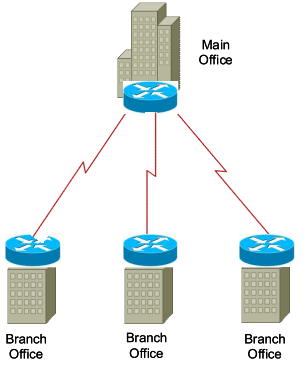
\includegraphics[scale=1]{figures/ex/cmo.png}
\caption{Connection to the Main Office}
\end{figure}

"\`E stata progettata una rete di una piccola compagnia con una topologia gerarchica \textit{Hub-And-Spoke}. La LAN in ogni ufficio secondario è connessa all'ufficio principale tramite un router ed un link con capacità $C = 128\ Kbps$. Dove $(1\ Kbit = 1000\ bits)$. In uno dei siti il flusso del traffico in uscita è generato principalmente da applicazioni CAD fino ad adesso. Per quel traffico, che può essere modellato come un processo di Poisson con rate $\lambda_0 = 3\ pkt/s$, è richiesto che il queueing delay nel router (per i pacchetti in coda) sia meno di $0.5$ secondi con probabilità più grande di $0.99$. A seguito di una nuova configurazione dei processi di business, è anche necessario installare un numero di computer per l'automazione degi uffici. Ci si aspetta che ognuno di loro generi un flusso di pacchetti verso l'ufficio centrale ad un average rate di $\lambda = 1\ pkt/s$. Per quest'ultimo flusso, è richiesto che l'average time speso nel router sia minore od uguale ad 1s.

Le dimensioni dei pacchetti possono essere modellate da variabili casuali indipendenti che sono esponenzialmente distribuite con valore medio $D = 500bytes$.

\begin{itemize}
\item Si assuma che la coda di output del router abbia capacità infinita e sia condivisa da tutti i flussi di traffico secondo disciplina di coda FCFS. Si determini il massimo numero $M$ di nuovi computer che possono essere installati;
\item Considerando il valore $M$, si valuti la \textit{packet loss probability} nel caso la dimensione della coda di output sia limitata a 10 pacchetti.
\end{itemize}

Abbiamo una topologia Hub-And-Spoke. (centro-e-raggi, topologia stellare). $C = 128\ Kbps$. Dove $(1\ Kbit = 1000\ bits) \implies C = 128000\ bit/s$. $\lambda_o = 3\ pkt/s\ \land\ \lambda = 1\ pkt/s$. Si richiede che il ritardo di accodamento nel router sia minore di $0.5s$ con probabilità maggiore di $0.99$. Le lunghezze dei pacchetti sono distribuite esponenzialmente di media 500 bytes. Politica FCFS. Quanto è il numero massimo di computer installabili $M$?

Supponiamo di indicare con $W$ la v.a. che rappresenta il ritardo di accodamento; il vincolo è il seguente, con $(\tau = 0.5s),\ \underline{s=threshold}=0.99$:

\[
	\Pr\{W < (\tau = 0.5s)\ |\ si\ faccia\ coda\} > (0.99 = s)
\]

Indichiamo con $\bar{R}$ il ritardo di accodamento per l'ultimo flusso. Deve valere: $\bar{R} \leq 1s$. Cerchiamo di risolvere il sistema con M/M/1. Abbiamo già delle ipotesi, ma dovremo farne di aggiuntive. Modelliamo quindi il router con un sistema a coda M/M/1:

Abbiamo un buffer output, ed un trasmettitore collegato in serie che è associato al link di uscita. Ipotesi: flusso secondo il quale arrivano i pacchetti di POISSON (pacchetti applicazioni CAD). Stiamo trascurando il ritardo di elaborazione router.
Capacità di elaborazione talmente elevata da ritenersi trascurabile (NO BOTTLENECK). Inoltre: $(d = +\infty)$. Il router opera con FCFS (quella contemplata dal sistema a coda M/M/1). Ipotesi aggiuntiva: certo numero di flussi, $M$ riguardanti i computer dell'Office Automation. Processo degli arrivi di POISSON. Ipotesi di indipendenza abbastanza scontata, dal momento che i vari utenti non si influenzeranno a vicenda. $M\lambda$. Ipotesi aggiuntiva: supponiamo che gli arrivi dei pacchetti relativi ai computer Office Automation siano indipendenti da quelli delle applicazioni CAD. Effettuando il POOLING, abbiamo che la distribuzione risultante è sempre un processo di POISSON con parametro dato dalla somma dei parametri: $\lambda' = \lambda_0+M\lambda$. Quindi $\lambda'$ è la velocità di arrivo dei clienti nel sistema a coda, $\mu$ è la velocità di servizio del router, ovvero il numero medio di pacchetti elaborati dal router per unità di tempo quando il router è costantemente occupato. Abbiamo dei tempi di servizio indipendenti, identicamente distribuiti ed indipendenti dai tempi di interarrivo. Nel sistema i tempi di servizio corrispondono ai tempi di trasmissione. Questo tempo di servizio è legato al parametro (valore medio) $D$ della distribuzione esponenziale che caratterizza la lunghezza dei pacchetti. Quindi abbiamo che il tempo medio di trasmissione è $\frac{1}{\mu} = \frac{D}{C} [s]$, ed abbiamo quindi $\mu = \frac{C}{D} = \frac{1}{D/C} = 32\  [pkt/s]$, ovvero abbiamo 32 pacchetti in media quando il router è costantemente occupato.

\begin{itemize}

\item{\textbf{Parte 1}}

Tutte le ipotesi del sistema a coda M/M/1 sono rispettate. Possiamo quindi utilizzarne i risultati: $\{\lambda',\mu\}$. Dobbiamo andare ad imporre quelle due condizioni. Per un M/M/1, il ritardo per cliente è $\bar{R} = \frac{1}{(\mu-\lambda)}$. Il ritardo per cliente è una v.a. distribuita esponenzialmente $\iff [R \sim EXP(\mu-\lambda)]$. Guardando adesso all'altra condizione, si dimostra che:

\[
	[F_W(y) = \Pr\{W \leq y\} = 1-\rho\e^{-\mu(1-\rho)y},\ y\geq 0]
\]

Tale è la CDF del Ritardo del cliente nella CODA! (Nella sola coda). $W$ sarebbe il tempo di permanenza del cliente nella SOLA coda del sistema a coda M/M/1. Distribuzione valutata su tutti i clienti (anche per quelli che non ci interessano). Dobbiamo condizionarla al fatto che si faccia coda. Quando $(y=0)$, esce $\Pr\{W\leq 0\} = (1-\rho)$. Ovvero la probabilità che il tempo di permanenza in fila di attesa sia nullo è pari a $(1-\rho)$. $\Pr\{W = 0\} = 1-\rho$. Si tratta di una v.a. mista. $\rho$ è il fattore di utilizzazione del router. Nel sistema a coda M/M/1, $\rho = (\frac{\lambda'}{\mu})$. Nell'M/M/1, $(1-\rho)=\pi_0^{(a)}$, ovvero la frazione di tempo a regime nel quale nel sistema a coda non vi sono clienti. La probabilità che il tempo di permanenza sia nullo è PARI alla probabilità che all'arrivo la fila di attesa SIA VUOTA!

\[
	[\Pr\{W = 0\} = 1-\rho = \pi_0]
\]

Questa è pari alla probabilità che un cliente AL SUO ARRIVO vada subito al router. In generale: $\pi_i^{(a)} \neq \pi_i$, laddove il primo membro della disuguaglianza riflette la visione dei clienti all'arrivo, valutata solo sugli istanti di arrivo, mentre il secondo membro riflette la visione all'esterno del sistema, considerando tutto l'asse temporale. $\pi_i$, ponendo l'ERGODICIT\`A, rappresenta la frazione di tempo nel quale vi sono $i$ clienti a regime. Mentre $\pi_i^{(a)}$ è la probabilità calcolata valutando SOLTANTO GLI ISTANTI DI ARRIVO! Frazione degli ARRIVI che trovano il sistema (a regime) nello stato $i$. Infatti potremmo avere ad esempio: $\{\{\pi_1 = \frac{1}{3},\ \pi_0=\frac{2}{3}\}\ \land\ \{\pi_0^{(0)}=1,\ \pi_1^{(0)}=0,\ \pi_2^{(0)}=0\}\}$.

\begin{thrm}{\textbf{P.A.S.T.A. \textit{POISSON ARRIVALS SEE TIME AVERAGES}}}

\[
	\left\{
	\begin{aligned}
	&\pi_i = \lim_{t\to\infty}{\Pr\{N(t)=i\}}\\
	&\pi_i^{(a)} = \lim_{t\to\infty}{\Pr\{N(t)=i\ |\ un\ arrivo\ subito\ dopo\ t\}}
	\end{aligned}
	\right.
\]

Se gli arrivi dei clienti si susseguono con processo di POISSON, abbiamo che: $\pi_i^{(a)}=\pi_i,\ \bar{N}=\sum_{i=0}^\infty{i\pi_i}$

\end{thrm}

Dove la prima equazione è una quantità calcolata sull'insieme delle realizzazioni. (Media di insiemi). Ma se vale L'ERGODICIT\`A, allora le medie d'insieme coincidono con le medie TEMPORALI. $\pi_i$ rappresenta la frazione del tempo nella quale vi sono a regime $i$ clienti nel sistema; $\pi_i^{(a)}$ rappresenta la frazione dei clienti che, all'arrivo trovano il sistema nello stato $i$. Coincide con la probabilità (a regime), che all'arrivo un cliente trovi $i$ clienti nel sistema. Rappresenta cosa vedono i clienti all'arrivo.

Per i nostri scopi, $[\pi_0^{(a)} = \Pr\{W = 0\}] = [\underline{1-\rho = \pi_0}]$, ove la parte sottolineata è la probabilità che vi siano 0 clienti, in un istante qualsiasi, mentre il primo membro è la probabilità che un cliente, al suo arrivo, trovi 0 clienti nel sistema. Grazie al teorema appena visto, esse coincidono. 

$\rho$ è la frazione del tempo in cui il router è occupato $\implies$ probabilità che il router sia occupato. $(1-\rho)$ è la probabilità che il router sia quindi libero. 
$\Pr\{W \leq \tau\ |\ si\ fa\ coda\} = (\dots)$ è la probabilità che il tempo di permanenza in FILA DI ATTESA sia inferiore (od uguale) a $\tau$, quando si fa coda.
Quindi abbiamo:

\[
	(\dots) = 1-\Pr\{W > \tau\ |\ si\ fa\ coda\} = 1-\frac{\Pr\{W > (y := \tau),\ si\ fa\ coda\}}{\Pr\{si\ faccia\ coda\}} = (\dots)
\]

Notiamo che $\{W > y\} \supseteq \{si\ fa\ coda\}$, ed inoltre, dal teorema appena visto (PASTA) vale che: $1-\pi_0^{(a)} = 1-\pi_0 = \rho = \Pr\{si\ fa\ coda\}$, ovvero la probabilità che all'arrivo di un cliente il servitore sia occupato coincide con la probabilità di fare coda. Ciò implica: $\implies$

\[
	(\dots) = 1-\frac{\Pr\{W>\tau\,\ si\ fa\ coda\}}{\Pr\{si\ fa\ coda\}} = 1-\frac{\Pr\{W\geq\tau\}}{\rho} =
\]
\[
	= 1-\frac{\rho\e^{-\mu(1-\frac{\lambda}{\mu})y}}{\rho} = 1-\e^{-\mu(1-\frac{\lambda}{\mu})y},\ y\geq 0
\]

Concludiamo che:

\[
	\Pr\{W \leq y\ |\ si\ fa\ coda\} = 1-\e^{-\mu(1-\frac{\lambda}{\mu})y} \iff W|_{\{si\ fa\ coda\}} \sim EXP(\mu-\lambda)
\]

quindi nell'M/M/1, $R=W|_{\underline{\{si\ fa\ coda\}}}$. Si riferisce proprio alla medesima distribuzione esponenziale, con il medesimo parametro!

Consci che $[R = \frac{1}{\mu-\lambda'}]$, allora procediamo:

\[	
	1-\e^{-(\mu-\lambda')\tau} > s \implies \e^{-(\mu-\lambda')\tau} < (1-s) \implies -(\mu-\lambda')\tau < \log(1-s) \implies (\dots)
\]
\[
	(\dots) \implies -\mu\tau +\lambda'\tau < \log(1-s) \implies [\lambda'\tau < \log(1-s)+\mu\tau] \implies (\dots)
\]
\[
	(\dots) \implies \lambda_0+M\lambda < \frac{\log(1-s)}{\tau} + \mu \implies M\lambda < \mu + \frac{\log(1-s)}{\tau}-\lambda_0 \implies (\dots)
\]
\[
	(\dots) \implies M < \frac{1}{\lambda}[\mu+\frac{1}{\tau}\log(1-s)-\lambda_0] = [32.8]
\]

ove il valore si è ottenuto appositamente sostituendovi i dati al secondo membro dell'ultima disequazione.

Quindi $\floor{M} = M_{max} = 32$ computer massimi.
Si ottiene $M \leq 32.8$, quindi possiamo installare MASSIMO 32 COMPUTER. D'altro canto dobbiamo rispettare anche il vincolo sull'average router time:

\[
	\bar{R} = \frac{1}{\mu-\lambda'} \implies \frac{1}{\mu-\lambda'} \leq 1s \implies ((\mu-\lambda')>0) \geq 1s \implies (\dots)
\]

ove l'ultima parentesizzazione maggiore di 0 indica la condizione di STABILIT\`A, che naturalmente deve essere sempre rispettata.

\[
	(\dots) \implies \mu - (\lambda_0+M\lambda)\geq 1 \implies \mu-\lambda_0 -M\lambda \geq 1 \implies M\leq\frac{\mu-\lambda_0-1}{\lambda} =
\]
\[
	= \frac{1}{\lambda}[\mu-\lambda_0-1] \implies M\leq 28
\]

Ne si conclude che $M_{max}=\min{\{28,32\}} = 28$ computer. Quindi: $\underline{\underline{[M\leq M_{max}=28]}}$.


\newpage

\item{\textbf{Parte 2}}: 

\subsubsection{M/M/1/k}

Consideriamo che $d = 10\ pkt$ (10 pacchetti), $d<+\infty$ ed abbiamo quindi un buffer di dimensione finita. $\iff (d=10)<+\infty$. In questo caso NON possiamo studiare il sistema con un modello M/M/1! Ci serve invece un \textit{M/M/1/k}, nel quale la dimensione del buffer è limitata. Pensiamo a $k$ come la capacità di tutto il sistema (includendo il centro di servizio). Stiamo quindi considerando un sistema a CODA CON PERDITA. Quando un elemento arrivando trova la coda piena, il sistema interviene con il meccanismo di DISCARD (avviene il fenomeno \textit{packet loss}). In questo caso $\lambda'$ è la velocità di arrivo dei clienti al sistema (POISSON). $\lambda_s$ sarà sempre la velocità di ingresso alla coda e di uscita (numero medio di clienti). $\rho=\frac{\lambda_s}{\mu}$ è il fattore di utilizzazione del servitore. Abbiamo che:

\[
	\Pr\{perdita\} = \frac{\lambda^l}{\lambda'} = \pi_k^{(a)} = \pi_k
\]

grazie a PASTA. Disegnamo il relativo DTT della catena:

\begin{center}
\begin{tikzpicture}[->, >=stealth', auto, semithick, node distance=2cm]
\tikzstyle{every state}=[fill=white,draw=black,thick,text=black,scale=1]
\node[state]    (0)                     {$0$};
\node[state]    (1)[right of=0]   {$1$};
\node[state]    (2)[right of=1]   {$2$};
\node[state] (d) [right of=2] {\ldots};
\node[state]    (km1)[right of=d]   {$k-1$};
\node[state]    (k)[right of=km1]   {$k$};
\path
(0) edge[bend left]     node{$\lambda'$}         (1)
(1) edge[bend left]     node{$\lambda'$}         (2)
    edge[bend left,below]    node{$\mu$}            (0)
(2) edge[bend left]     node{$\lambda'$}           (d)
    edge[bend left,below]    node{$\mu$}             (1)
(d) edge[bend left]         node{$\lambda'$}   (km1)
	edge[bend left,below]   node{$\mu$}          (2)
(km1) edge[bend left]       node{$\lambda'$}  (k)
	  edge[bend left,below]   node{$\mu$}     (d)
(k)   edge[bend left,below]  node{$\mu$}          (km1);
\end{tikzpicture}
\end{center}

Sia $N(t)$ il numero di clienti nel sistema a tempo $t$. 
$\Pr\{\phi_i(t) > \tau\} = (\dots)$, dove $\phi_i(t)$ indica il tempo di soggiorno residuo nello stato $i$ al tempo $t$, indica la probabilità che per almeno $\tau$ unità di tempo non ci sia alcun arrivo e NON vi sia la fine del servizio in corso, condizionata con il fatto che attualmente vi sono $i$ clienti nel sistema.

Indichiamo con $\xi_{Rt} \sim EXP(\lambda')$ la v.a. tempo di interarrivo residuo al tempo $t$, e con $\eta_{Rt} \sim EXP(\mu)$ la v.a. tempo di servizio residuo al tempo $t$. Tutte indipendenti ed indipendenti tra di loro, grazie all'ipotesi di (inter)-indipendenza. 

\[
	(\dots) = \Pr\{\xi_{Rt}>\tau,\ \eta_{Rt}>\tau\} = \Pr\{\xi_{Rt}>\tau\}\Pr\{\eta_{Rt}>\tau\} = \e^{-\lambda'\tau}\e^{-\mu\tau} = \e^{-(\lambda'+\mu)\tau}
\]

Quindi abbiamo di nuovo: $-q_{ii} = \mu+\lambda' \implies$

\[
	\tau_{i,i+1} = \frac{q_{i,i+1}}{-q_{ii}} = \frac{q_{i,i+1}}{(\mu+\lambda')}
\]

$\tau_{i,i+1}$ è la probabilità che lasciando lo stato $i$, il processo vada verso $i+1$. Sfruttando il teorema delle probabilità totali nel continuo, abbiamo: $q_{i,i+1} = (\mu+\lambda') \frac{\lambda'}{(\mu+\lambda')} = \lambda'$. Quindi sarà $\lambda'$ fino a $k-1$. La CMTC è una catena omogenea, IRRIDUCIBILE e dal momento che $\cardinality{stati}<+\infty \implies$ allora essa è SICURAMENTE ERGODICA! CATENA SEMPRE ERGODICA. Sistema STABILE.

\[
	\left\{
	\begin{aligned}
	&[\pi_i = \pi_0(\frac{\lambda'}{\mu})^i]\\
	&[\pi_0 = \frac{1}{1+\sum_{i=1}^k{(\frac{\lambda'}{\mu})^i}}]
	\end{aligned}
	\right.
\]

$i=1,2,\ \dots,\ k$.

Notiamo che:

\[
	\sum_{i=0}^k{\rho^i} = \left\{
	\begin{aligned}
	&k+1,\ \rho=1\\
	&\frac{1-\rho^{k+1}}{(1-\rho)},\ p\neq 1
	\end{aligned}
	\right.
\]

Quindi nel nostro caso abbiamo:

\[
	\pi_0 = \frac{1}{\sum_{i=0}^k{\rho^i}} = \frac{1}{\frac{1-\rho^{k+1}}{(1-\rho)}} = \frac{1-\rho}{1-\rho^{k+1}}
\]

Quindi abbiamo come Distribuzione di regime:

\[
	\pi_i = \frac{1-\rho}{1-\rho^{k+1}} \rho^i,\ i=0,1,2,\ \dots,\ k
\]

Si noti che vale anche per $i=0$. Allora:

\[
	[\Pr\{perdita\} = \underline{\pi_k^{(a)} \stackrel{PASTA}{=} \pi_k} = [\frac{1-\rho}{1-\rho^{k+1}} \rho^k]]
\]

da valutarsi con $k=10+1=d+1<+\infty$, in quanto include anche il centro di servizio.
Facendo i calcoli esce $0.07 \implies (70\%)$.

La probabilità di perdita si poteva trovare, come precedentemente enunciato, anche effettuando il rapporto $\frac{\lambda_L}{\lambda'}$. Banalmente, per SPLITTING si ha: $[\lambda_L=\lambda'-\lambda_S]$. Le perdite comunque mi fanno venire meno la caratteristica di POISSON.

\[
	\Pr\{k\ arrivi\ in\ \tau\} = \frac{(\lambda\tau)^k}{k!}\e^{-\lambda\tau}
\]

ma la sequenza degli ingressi a valle della diramazione NON è più di POISSON! $\rho = (\frac{\lambda_S}{\mu})$ rappresenta il fattore di utilizzazione, quindi la frazione del tempo a regime in cui il servitore è occupato. $\rho=1-\pi_0 \implies \pi_0=1-\rho$.

$\lambda_S=\mu(1-\pi_0)$ rappresenta la velocità delle partenze (\textit{departure}) dei clienti dal mio sistema. Abbiamo: $[\pi_0 = \frac{1-\rho}{1-\rho^{k+1}}]$.

\[
	\lambda_L = \lambda'-\lambda_S = \lambda'-\mu(1-\pi_0)
\]

Quindi $\lambda_S$ è la velocità secondo la quale i clienti partono dal sistema, od anche la media dei clienti che partono all'unità di tempo. Guardando il DTT, vi è una partenza quando FINISCE un servizio! Determinando le frequenze delle transizioni a sinistra, potremo sapere le frequenza delle partenze. La frequenza delle partenze si ottiene sommando tutte le frequenze delle transizioni $\pi_iq_{ij}$, sfruttando opportunamente l'inversa della CONDIZIONE DI \underline{NORMALIZZAZIONE}:

\[
	\pi_1\mu + \pi_2\mu +\ (\dots)\ +\pi_k\mu = \mu\sum{\pi_i} = [\lambda_S = \mu(1-\pi_0)]
\]

Stessa cosa mettendoci a valle della diramazione ed a monte della coda: (ARRIVI DI CLIENTI dall'esterno del sistema). $\lambda_S$ rappresenta qui il numero medio di clienti che entrano nel sistema per unità di tempo.

\[
	\lambda_S = [\pi_0\lambda'+\pi_1\lambda'+\ \dots\ +\pi_{k-1}\lambda'] = \lambda'
\]

Valgono le equazioni di bilanciamento locale, valide solo per una CMTC di nascita e morte (BDCMTC):

\[
	\pi_1\mu = \pi_0\lambda' \implies \pi_{k+1}\mu = \pi_k\lambda'
\]

ovvero le sommatorie sono identiche.

$\frac{\lambda_L}{\lambda'}$ rappresenta la probabilità di perdita.

\begin{thrm}{\textbf{Probabilità di perdita}}

\[
	\Pr\{perdita\} = \frac{1-\rho}{1-\rho^{k+1}}\rho^k = \pi_k^{(a)} = \pi_k
\]

ove $\pi_k$ rappresenta la probabilità che il sistema si trovi nello stato $k$ in un istante qualsiasi. Abbiamo anche:

\[
	\Pr\{perdita\} = \frac{(\lambda_L = \lambda'-\lambda_S)}{\lambda'} = 1-\frac{\lambda_S}{\lambda'} = (\dots)
\]
\end{thrm}

Ove $\lambda_S$ è stato trovato applicando Little al primo sottosistema, ottenendo quindi $\lambda_S =\mu(1-\pi_0)$.

\begin{proof}

\[
	(\dots) = 1-\frac{\mu(1-\pi_0)}{\lambda'} = 1-\frac{1}{\rho}(1-\frac{1-\rho}{1-\rho^{k+1}}) = 1-\frac{1}{\rho}(\frac{1-\rho^{k+1}-1+\rho}{1-\rho^{k+1}})
\]
\[
	1-\frac{1}{\rho}\rho \frac{(1-\rho^k)}{(1-\rho^{k+1})} = \frac{1-\rho^{k+1}-1+\rho^k}{1-\rho^{k+1}} = \frac{\rho^k(1-\rho)}{(1-\rho^{k+1})};
\]

\end{proof}

La probabilità di perdita di un cliente deve quindi alla fine coincidere con il rapporto $\frac{\lambda_L}{\lambda'}$.

\end{itemize}

\subsection{Sistemi a coda M/M/m}

Il sistema a coda M/M/m rappresenta una generalizzazione del sistema M/M/1. Abbiamo $m$ router.
Anche in questo caso, il processo degli arrivi è un processo di POISSON con velocità $\lambda$. ($\lambda$ = velocità di arrivo dei clienti). In media arrivano $\lambda$ clienti per unità di tempo. Anche in questo caso i tempi di servizio sono v.a. indipendenti (mutuamente), i.d. con una distribuzione esponenziale negativa unilatera, con tempo medio di servizio $(\frac{1}{\mu})$, ed indipendenti statisticamente dai tempi di interarrivo dei clienti nel sistema a coda. La velocità del centro di servizio sarà variabile (il centro di servizio include ora $m$ servitori), ovvero dipende dal numero di router attivi in un certo istante di tempo. Se $i$ è il numero di clienti nel sistema a coda in un certo istante di tempo, $i<m \implies i\mu$ velocità del centro di servizio. $i$ sono i clienti IN TUTTO IL SISTEMA! In totale quindi i servitori attivi serviranno $i\mu$ utenti $\forall$ unità di tempo. $i\geq m$ tutti gli $m$ servitori saranno attivi $\implies$ velocità $m\mu$. Quindi $i\geq m$ centro di servizio alla massima velocità possibile. $m\mu$ = capacità TOTALE DI SERVIZIO DEL SISTEMA (del centro di servizio). Come nella M/M/1, la dimensione del buffer e la popolazione sono illimitate ($\iff d,e<+\infty$). Disciplina di queueing di default (FCFS). Modellabile come uno stack FIFO. Se arriva un cliente e c'è un certo numero di router liberi, sarà assegnato in maniera random ad uno di questo. Approccio MARKOVIANO basato sul processo stocastico che si riferisce al numero di clienti nell'intero sistema a coda al tempo $t$, ovvero $N(t)$. La sua evoluzione sarà determinata dalle v.a. tempi di interarrivo e tempi di servizio. Dato che per queste ipotesi queste v.a. sono prive di memoria e statisticamente indipendenti $\implies$ siamo dinanzi una CMTC, il cui diagramma dei tassi di transizione è il seguente:

\begin{center}
\begin{tikzpicture}[->, >=stealth', auto, semithick, node distance=2cm]
\tikzstyle{every state}=[fill=white,draw=black,thick,text=black,scale=0.8]
\node[state]    (0)                     {$0$};
\node[state]    (1)[right of=0]   {$1$};
\node[state]    (2)[right of=1]   {$2$};
\node[state] (d) [right of=2] {\ldots};
\node[state]    (mm1)[right of=d]   {$m-1$};
\node[state]    (m)[right of=mm1]   {$m$};
\node[state]    (mp1)[right of=m]   {$m+1$};
\node[state]    (mp2)[right of=mp1]   {$m+2$};
\node[state]    (d2)[right of=mp2]  {\ldots};

\path
(0) edge[bend left]     node{$\lambda$}         (1)
(1) edge[bend left]     node{$\lambda$}         (2)
    edge[bend left,below]    node{$\mu$}            (0)
(2) edge[bend left]     node{$\lambda$}           (d)
    edge[bend left,below]    node{$2\mu$}             (1)
(d) edge[bend left]         node{$\lambda$}   (mm1)
	edge[bend left,below]   node{$3\mu$}          (2)
(mm1) edge[bend left]       node{$\lambda$}  (m)
	  edge[bend left,below]   node{$(m-1)\mu$}     (d)
(m)   edge[bend left]   node{$\lambda$}      (mp1)
      edge[bend left,below]  node{$m\mu$}          (mm1)
(mp1) edge[bend left]       node{$\lambda$}  (mp2)
	 edge[bend left,below]   node{$m\mu$}      (m)
(mp2) edge[bend left]       node{$\lambda$}   (d2)
      edge[bend left,below] node{$m\mu$}    (mp1)
(d2) edge[bend left,below]   node{$m\mu$}     (mp2);
\end{tikzpicture}
\end{center}

CMTC nascita e morte (BDCMTC), con $\cardinality{stati}=+\infty$ (infiniti), fila di attesa di dimensione illimitata. Tassi di nascita pari a $\lambda$, tassi di morte $m\mu$, che sarebbe il tasso di morte nello stato $i$ prima che si saturino i servitori disponibili, dopodiché $(i\geq m)$, sempre pari a $m\mu$.

\subsubsection{Calcolo dei tassi (velocità) di transizione}

Supponiamo $N(t)=i\neq 0$ ($i$ clienti nel mio intero sistema a coda), ovvero qualsiasi stato diverso dallo stato banale. Il successivo cambiamento di stato sarà legato od all'arrivo di un nuovo cliente od al completamento di uno dei servizi eseguiti in parallelo al tempo $t$. Comunque abbiamo $i$ clienti totali. Possibili casi: $\{i++,\ i--\}$. L'intervallo di tempo da $t$ al successivo arrivo lo indichiamo con $\underline{\xi_R(t) \sim EXP(\lambda)}$, ovvero il tempo di interarrivo residuo (stessa caratteristiche dei tempi di interarrivo). Il tempo che passa tra l'istante presente $t$ ed il successivo completamento del servizio, sarà $\eta_R(t)$, e sarà pari al minimo dei tempi di servizio residui in $t$. Ci saranno un certo numero di servizi. $\eta_R(t) = \min{\{...\}}$, ovvero al minimo dei tempi di servizio residui legati a quei servizi che al tempo $t$ stanno procedendo in parallelo. Quando $i<m$, ci saranno $i$ servizi che stanno procedendo in parallelo. Anche i tempi di servizio residui sono \underline{indipendenti} fra di loro per ipotesi, dal momento che i servizi procedono in parallelo senza influirsi. Quindi $\eta_R(t) \sim EXP(\sum_i{\mu_i})$. Quando $i<m\implies$ $\eta_R(t) \sim EXP(i\mu)$. Se invece $i\geq m$, $\eta_R(t) \sim EXP(m\mu)$. A questo punto, il tempo che passa dall'istante presente $t$ e la successiva transizione di stato, sarà $\phi_i(t)$ (tempo di soggiorno residuo nello stato $i$ al tempo $t$) prima di cambiare stato $\implies$

\[
	\phi_i(t) = \min{\{\xi_R(t),\ \eta_R(t)\}} \implies \phi_i(t) \sim EXP(-q_{ii})
\]

ove l'ultima implicazione è valida grazie al fatto che queste variabili casuali sono i.i.d. ed indipendenti tra di loro. Abbiamo:

\[
	-q_{ii} = \left\{
	\begin{aligned}
	&(\lambda+i\mu),\ i<m\\
	&(\lambda+m\mu),\ i\geq m
	\end{aligned}
	\right.
\]

(Velocità totale di uscita \underline{dallo stato i}). Parametro $-q_{ii}$. Quindi, quella quantità rappresenta con che velocità in totale esco dallo stato. Ma se $\underline{i<m}$, perché $q_{i,i+1} = \lambda,\ q_{i,i-1}=i\mu$. Solito giochetto. (Se $i\geq m,\ q_{i,i-1}=m\mu$). Consideriamo:

\[
	\tau_{i,i+1} = \frac{q_{i,i+1}}{-q_{ii}} = \Pr\{\xi_R(t) < \eta_R(t)\} = (\dots)
\]

ove l'ultima quantità rappresenta la probabilità che il prossimo arrivo preceda la fine del servizio (il completamento del servizio). Dobbiamo quindi applicare il teorema delle probabilità totali nel continuo, ottenendo alla fine:

\[
	(\dots) = \left\{
	\begin{aligned}
	&\frac{\lambda}{\lambda+i\mu},\ i<m\\
	&\frac{\lambda}{\lambda+m\mu},\ i\geq m
	\end{aligned}
	\right.
\]

CMTC OMOGENEA, IRRIDUCIBILE, ma non sappiamo tuttavia se è ERGODICA.

\[
	\left\{
	\begin{aligned}
	&[\pi_0 = \frac{1}{1+\sum_{i=1}^{m-1}{(\frac{\lambda}{\mu})^i\frac{1}{i!}} + (\frac{m^m}{m!})\sum_{i=m}^\infty{(\frac{\lambda}{m\mu})^i}}]\\
	&\left\{
	\begin{aligned}
	&\pi_i = \pi_0 (\frac{\lambda}{\mu})^i \frac{1}{i!},\ i<m\\
	&\pi_i = \pi_0 (\frac{\lambda}{\mu})^i \frac{1}{m!m^{i-m}},\ i\geq m
	\end{aligned}
	\right.
	\end{aligned}
	\right.
\]

Dobbiamo capire qual'è la CONDIZIONE MAX di ERGODICIT\`A (si ha una condizione di regime). La sommatoria ad infiniti termini (serie) a denominatore di $\pi_0$ deve convergere di nuovo. La condizione di ERGODICIT\`A è quindi: $(\frac{\lambda}{m\mu}) < 1$ (convergenza della serie geometrica). Quando $\rho := \frac{\lambda}{m\mu} < 1$ questa sommatoria (serie) converge, e si ha una distribuzione che è quella di regime. $[\lambda < m\mu]$ è proprio la condizione di STABILIT\`A, la quale indica che la velocità di arrivo deve essere minore della capacità totale di servizio. Serve sostanzialmente per evitare l'"ingolfamento". $\rho$ è il fattore di utilizzazione del generico router (Non del centro di servizio). Ognuno dei router avrà un fattore di utilizzazione pari a $\rho$, quando il carico è EQUAMENTE DISTRIBUITO. $\frac{\lambda}{m}$ sarà la capacità di arrivo del singolo cliente. Servono in media lo stesso numero di clienti $\forall$ unità di tempo. Tutti lavoreranno alla stessa maniera. Ogni router si vedrà arrivare quindi $\frac{\lambda}{m}$ clienti per unità di tempo. Fattore di utilizzazione; frazione di tempo quando il servitore è occupato. Infatti, applicando \underline{Little} troviamo: $(\frac{\lambda}{m})(\frac{1}{\mu})$, trovando la frazione di tempo nel quale il router è occupato per unità di tempo nella quale il router è costantemente occupato, quando il carico di lavoro è EQUAMENTE DISTRIBUITO. $\frac{\lambda}{\mu}$ è l'\textit{intensità di traffico} (arrivano $\lambda$ clienti, $\frac{1}{\mu}$ è il lavoro medio richiesto dal cliente). Quindi sfruttiamo ancora Little e troviamo: $\lambda(\frac{1}{\mu})$, trovando così il \underline{\underline{CARICO MEDIO DI LAVORO}}. 

\[	
	[\frac{\lambda}{\mu} = m(\rho := \frac{\lambda}{m\mu}) = m\rho]
\]

Si usi questo fatto per vedere a cosa converge la sommatoria geometrica:

\[	
	[\pi_0 = \frac{1}{\sum_{i=0}^{m-1}{(m\rho)^i \frac{1}{i!}} + (\frac{m^m}{m!} \frac{\rho^m}{1-\rho} = \frac{(m\rho)^m}{m!(1-\rho)})}]
\]

e tramite questa espressione possiamo ovviamente trovare le $\pi_i$.

ERGODICIT\`A se: $[\underline{\lambda < m\mu}]$. Abbiamo trovato la distribuzione di regime. Nel caso M/M/1, abbiamo poi ricavato tutti i numeri medi di clienti e tempi di servizio, etc. Nel caso M/M/1 siamo partiti da $\bar{N}$.

\subsubsection{Quantità medie tipiche}

Adesso partiamo da $\bar{T}$, ovvero il ritardo medio per cliente a regime. Terminologia tempo di risposta. $\bar{T}$ tempo di risposta. Tempo di permanenza del cliente nel sistema a coda. Abbiamo:

\[
	(\bar{T} := \E[T]) = \E[t_s] + \E[W] = \frac{1}{\mu} + (\dots)
\]

ove $W$ è il tempo di accodamento, ovvero il queueing delay. Adesso per valutare il tempo medio di permanenza in fila di attesa utilizziamo il concetto di \textit{MEDIA CONDIZIONATA}:

\[
	(\dots) = \E[\E[W\ |\ k\ clienti\ all'arrivo]] = \mathord{\cdot}(k)
\]

dove $\{k\ clienti\ all'arrivo\}$ sarebbe l'evento nel quale troviamo $k$ clienti all'arrivo in testa al sistema. Tempo di permanenza, sapendo che all'arrivo il cliente trova $k$ clienti nel sistema. Quindi:

\[
	\bar{T} = \frac{1}{\mu} + \sum_{k=m}^\infty{\E[W\ |\ k\ clienti\ all'arrivo]}\pi_k^{(a)}
\]

Notiamo che $k$ parte da $m$, perché se $k<m$ quella quantità sarebbe nulla!
Il tempo medio di permanenza nella fila di attesa è nullo quindi se $k<m$! Se arrivato nel sistema a coda trovo un numero $(k<m)$ di clienti, allora VADO DIRETTAMENTE nel CENTRO DI SERVIZIO! Sommatoria che parte da $m$ quindi. Volendo la si potrebbe fare partire da 0, senza alcuna perdità di generalità, dal momento che i primi $(m-1)$ termini sarebbero comunque nulli. Abbiamo:

\[	
	\bar{T} = \frac{1}{\mu} + \sum_{k=m}^\infty{\frac{k-m+1}{m\mu}(\pi_k^{(a)}=\pi_k)} = (\dots)
\]

Dove l'uguaglianza tra parentesi deriva da PASTA. Abbiamo sfruttato il fatto che: $[\E[W|k] = \frac{k-m+1}{m\mu}]$. Siamo nel caso $k\geq m$, ove vi sono $m$ clienti al servizio, $(k-m)$ clienti in fila di attesa ed io. Dopo che vi sarà il completamento di $(k-m)$ servizi mi troverò in testa alla fila di attesa. Ma dovrò quindi attendere il completamento di un ulteriore servizio (ecco perché il termine $+1$). Ma il tempo tra il completamento del servizio corrente ed il successivo è $(\frac{1}{m\mu})$! ($\leftarrow$ tempo medio di servizio). $\implies$

\[
	(\dots) = \frac{1}{\mu} + \sum_{k=m}^\infty{(\frac{k-m+1}{m\mu})\pi_0\frac{m^m}{m!}\rho^k} = \frac{1}{\mu} + \pi_0\frac{m^m}{m!}\sum_{k=m}^\infty{\frac{k-m+1}{m\mu}\rho^k} = (\dots)
\]

A questo punto possiamo porre: $i := k-m+1$, ed otteniamo:

\[
	(\dots) = \frac{1}{\mu} + \pi_0\frac{m^m}{m!m\mu}\sum_{i=1}^\infty{i(\rho^{i-1+m} = \rho^{i-1}\rho^m)} =
\]
\[
	= \frac{1}{\mu} + \frac{(m\rho)^m}{m!m\mu}\pi_0\sum_{i=1}^\infty{i\rho^{i-1}} = [\frac{1}{\mu} + \frac{\pi_0(m\rho)^m}{m!m\mu} \frac{1}{(1-\rho)^2}]
\]

Abbiamo quindi trovato il RITARDO MEDIO PER CLIENTE. Volendo potremmo anche trovare con Little: $\bar{N}=\lambda\bar{T} = (\dots)$. Spesso in letteratura si esprime $\bar{T}$ in funzione della probabilità di attesa:

\[
	\Pr\{accodamento\ (queueing)\} = \sum_{k=m}^\infty{(\pi_k^{(a)}=\pi_k)}
\]

sarebbe ovvero la sommatoria di queste probabilità. Si deriva quindi la \textit{C di ERLANG}. (La B di ERLANG è invece collegata alla probabilità di perdita (M/M/m/0)). 

Siamo in un sistema a coda M/M/m. Ritardo medio per cliente:

\[
	\left\{
	\begin{aligned}
	&\bar{T} = \frac{1}{\mu} + \frac{\pi_0(m\rho)^m}{m!m\mu} \frac{1}{(1-\rho)^2}\\
	&\rho = \frac{\lambda}{m\mu},\ \rho<1
	\end{aligned}
	\right.
\]

ove l'ultima equazione del sistema indica la condizione di \underline{STABILIT\`A}. Questa quantità ($\bar{T}$), viene solitamente espressa in letteratura in funzione della probabilità di ATTESA, nella quale dobbiamo considerare la situazione in cui abbiamo almeno $m$ clienti nel sistema a coda quando arriva un cliente:

\[
	\Pr\{queueing\} = \sum_{k=m}^\infty{(\pi_k^{(a)}=\pi_k)} = \sum_{k=m}^\infty{\pi_k} =
\]
\[
	\sum_{k=m}^\infty{\pi_0(\frac{\lambda}{m\mu} = \rho)^k \frac{m^m}{m!}} = \pi_0\frac{m^m}{m!}\sum_{k=m}^\infty{\rho^k} = (\dots)
\]

Siamo dinanzi una sommatoria geometrica, quindi:

\[
	(\dots) = \pi_0\frac{m^m}{m!} (\frac{\rho^m}{1-\rho}) = \frac{\pi_0(m\rho)^m}{m!(1-\rho)} := C(m,\frac{\lambda}{\mu})
\]

Abbiamo ottenuto quest'espressione $C(m,(\frac{\lambda}{\mu}))$, nota come funzione \textit{C di ERLANG} con parametro: $\{m,(\frac{\lambda}{\mu})\}$. Ci sono delle tabelle per questa formula. Abbiamo ricavato un modello per la M/M/m. Possono essere utilizzate per modellare quei sistemi di servizio che prevedono diverse risorse. Sistemi di servizio con un certo numero di risorse, corrispondenti ai router $(m)$, laddove $(i\geq m \implies\ queueing)$.

Modello M/M/m. Dobbiamo però ritrovare le ipotesi dietro all'M/M/m nel mondo reale. Call-center ad esempio. Processo secondo il quale si susseguono gli arrivi al sistema a coda dev'essere ben modellabile come un processo di POISSON. Durata media delle telefonate (tempi medi di servizio) $(\frac{1}{\mu})$. In un call center mi ritrovo queste ipotesi. Ci vorrebbero anche le ipotesi sulla dimensione del buffer e della popolazione. $(d,e = +\infty)$. Dimensionamento del numero massimo di operatori (servitori) in base ad un predeterminato massimo valore da non scavalcare relativo alla probabilità di accodamento. $\{\lambda,\frac{1}{\mu}\} \to m$. Problema di progetto. Potremo anche voler affrontare un problema di ANALISI. Durata media delle telefonate $(\frac{1}{\mu})$. [ANALISI $\rightarrow$ PROGETTO]. In funzione della C di ERLANG, troviamo il valore del ritardo medio per cliente:

\[
	\bar{T} = \frac{1}{\mu} + C\frac{1}{m\mu}(\frac{1}{1-\rho}),\ \rho<1
\]

Ricordiamo che $(C\ di\ ERLANG = \Pr\{queuing\})$. Adesso, noto il valore del ritardo medio per cliente, applico Little e trovo:

\[
	\bar{N} = \lambda\bar{T} = \frac{\lambda}{\mu} + C\frac{\lambda}{m\mu}(\frac{1}{1-\rho}) = [m\rho + C\rho(\frac{1}{1-\rho})]
\]

Troviamo ora il tempo medio di permanenza nella sola fila di attesa, dove $(\rho := \frac{\lambda}{m\mu})$:

\[
	\bar{W} = \bar{T} - (T_s = \frac{1}{\mu}) = C\frac{1}{m\mu}(\frac{1}{1-\rho})
\]

E adesso il numero medio di clienti nella sola fila di attesa, $\bar{N_q}$

\[
	[\bar{N_q} = \lambda\bar{W} = C\rho(\frac{1}{1-\rho})]
\]

Dove abbiamo nuovamente applicato Little al sottosistema costituito dalla sola fila di attesa. Ora passiamo al centro di servizio, ragionando con gli stessi argomenti:

\[
	\left\{
	\begin{aligned}
	&(T_s=\frac{1}{\mu})\\
	&\bar{N_s} = m\rho := \frac{\lambda}{\mu} = \lambda(\frac{1}{\mu})
	\end{aligned}
	\right.
\]

$\rho$ è il FATTORE DI UTILIZZAZIONE. A REGIME $(\rho<1)$. Ricordiamo che $\lambda$ è sempre la velocità di arrivo.

\subsubsection{Confronto tra tre sistemi MARKOVIANI}

Questi tre sistemi MARKOVIANI hanno la stessa capacità di servizio e stessa velocità tutti tra di loro:

\begin{itemize}

\item{1)}: Un singolo sistema M/M/1 con velocità di arrivo $m\lambda$ e velocità di servizio del singolo servitore pari a $m\mu$. Parametri: $\{m\lambda,m\mu\}$;
\item{2)}: $m$ code M/M/1, ogni coda con velocità di arrivo $\lambda$ e di servizio $\mu \implies\ \{m\lambda,m\mu\}$ come parametri;
\item{3)} Sistema M/M/m con velocità di arrivo $m\lambda$ ed $m$ servitori. Ricordiamo che qui vale:

\[
	[\frac{1}{\mu} + C\frac{1}{m\mu}(\frac{1}{1-\rho}) = \bar{T},\ (\rho<1)]
\]

Abbiamo parametri: $\{m\lambda,m\mu\}$.

\end{itemize}

Tre sistemi che hanno tutti la stessa velocità di arrivo e di servizio. Confrontiamo i ritardi medi di permanenza per i clienti. Dobbiamo quindi stilare una graduatoria:
Effettuiamo un confronto:

\[
	\left\{
	\begin{aligned}
	&\bar{T_1} = \frac{1}{m\mu-m\lambda} = \frac{1}{m(\mu-\lambda)}\\
	&\bar{T_2} = \frac{1}{\mu-\lambda}\\
	&\bar{T_3} = ?
	\end{aligned}
	\right.
\]

Dovremmo fare i conti con l'espressione di $\bar{T}$ precedentemente trovata. Ma, intuitivamente la classifica sarebbe: $\{1,3,2\}$. Il primo sarebbe il migliore, sebbene poco attuabile nella pratica. Ci accontentiamo del terzo sistema. Primo sistema non attuabile come umani come router. Il primo lavora sempre alla capacità di servizio, mentre il terzo ha capacità di servizio $m\mu$ solo quando $i\geq m$!

\subsubsection{M/M/m/0}

In questo sistema abbiamo 0 come dimensione del buffer \newline
$\iff (d=0)<+\infty$. \underline{\underline{NO POISSON modeling}}!
In letteratura troviamo anche M/M/m/m $(d=m)$. Nel primo caso con $d$ si intende la dimensione del buffer, mentre $(d=m)$ intende il numero totale di clienti nel sistema. Ovviamente M/M/m/0 $\neq$ M/M/m, in quanto se $i\geq m$, i clienti in arrivo vengono irrimediabilmente persi. $m$ router e velocità $\mu$ ciascuno $(\frac{1}{\mu})$ ritardo medio per cliente. v.a. memoryless EXP (UNI-NEG). statisticamente indipendenti i.d. ed indipendenti statisticamente dai tempi di interarrivo (MARKOV). $\lambda_D=\lambda_S$, dove $D$ sta per \textit{departure}. Si può verificare quindi il fenomeno di \underline{LOSS}. Sistema con blocco, ma con \underline{perdita} (Non si può fare fila in coda). $\lambda_S$ sarà anche la velocità di partenza! Le perdite fanno perdere la proprietà di POISSON per il processo che modella il numero di clienti. Di conseguenza il processo secondo il quale entrano i clienti nel centro di servizio NON è più di POISSON, il quale modellerebbe la distribuzione di massa in tal modo:

\[	
	\Pr\{k\ arrivi\ in\ \tau\} = \frac{(\lambda\tau)^k}{k!}\e^{-\lambda\tau}
\]

Ma in questo caso è 0 se $k\geq m$! $N(t)$ è il numero di clienti nel sistema a coda al tempo $t$. Sostanzialmente coincide con il numero di clienti nel centro di servizio del sistema. $\underline{\underline{N(t)}}$. Sia una CMTC, dal momento che abbiamo indipendenza tra $\lambda$ e $\mu$. Il diagramma DTT è il seguente:

\begin{center}
\begin{tikzpicture}[->, >=stealth', auto, semithick, node distance=2.3cm]
\tikzstyle{every state}=[fill=white,draw=black,thick,text=black,scale=1]
\node[state]    (0)                     {$0$};
\node[state]    (1)[right of=0]   {$1$};
\node[state]    (2)[right of=1]   {$2$};
\node[state]    (3)[right of=2]   {$3$};
\node[state] (d) [right of=3] {\ldots};
\node[state]    (mm1)[right of=d]   {$m-1$};
\node[state]    (m)[right of=mm1]   {$m$};

\path
(0) edge[bend left]     node{$\lambda$}         (1)
(1) edge[bend left]     node{$\lambda$}         (2)
    edge[bend left,below]    node{$\mu$}            (0)
(2) edge[bend left]     node{$\lambda$}           (3)
    edge[bend left,below]    node{$2\mu$}             (1)
(3) edge[bend left]     node{$\lambda$}           (d)
    edge[bend left,below]    node{$3\mu$}             (2)
(d) edge[bend left]         node{$\lambda$}   (mm1)
	edge[bend left,below]   node{$3\mu$}          (3)
(mm1) edge[bend left]       node{$\lambda$}  (m)
	  edge[bend left,below]   node{$(m-1)\mu$}     (d)
(m)   edge[bend left,below]  node{$m\mu$}          (mm1);
\end{tikzpicture}
\end{center}

Mi trovo dinanzi ad una catena di nascita e morte (BDCMTC) con insieme degli stati FINITO $(\iff \cardinality{stati}<+\infty)$. Abbiamo i seguenti tassi di transizione, trovati rispetto al DTT relativi all'M/M/m (lì avevamo però un numero di stati infinito):

\[
	\left\{
	\begin{aligned}
	&\lambda_i=\lambda\ \forall i=0,1,\ \dots,\ m-1\\
	&\mu_i = i\mu,\ i=1,\ \dots,\ m
	\end{aligned}
	\right.
\]

ove l'ultimo range di indici relativo al tassi di morte è tale per cui sarebbe 0 altrimenti. La catena è ERGODICA $\iff$ esiste sicuramente la distribuzione di regime:

\[
	\left\{
	\begin{aligned}
	&[\pi_i = \pi_0 (\frac{\lambda}{\mu})^i (\frac{1}{i!})],\ i=1,\ \dots, m\\
	&[[\pi_0 = \frac{1}{1+\sum_{k=1}^m{(\frac{\lambda}{\mu})^k (\frac{1}{k!})}}] = \frac{1}{\underline{\sum_{k=0}^m{(\frac{\lambda}{\mu})^k (\frac{1}{k!})}}}]
	\end{aligned}
	\right.
\]

ove nell'ultimo passaggio sottolineato dell'equazione abbiamo inglobato l'1 nella sommatoria. Ora sappiamo già che è ERGODICA (la sommatoria è una semplice SOMMA di un numero finito di elementi, quindi convergerà sicuramente).

\[
	[\pi_i = \frac{(\frac{\lambda}{\mu})^i (\frac{1}{i!})}{\sum_{k=0}^m{(\frac{\lambda}{\mu})^k (\frac{1}{k!})}}]
\]

$\leftarrow$ ovvero la probabilità di regime, per $\underline{0\leq i\leq m}$. Quando $(i=0)$, trovo esattamente $\pi_0$ in evidenza.

$\bar{N}$ sia il numero medio di clienti nel sistema. $\implies \bar{N}=\sum_{i=0}^m{i\pi_i}$. Possiamo applicare anche Little al centro di servizio: $\implies \bar{N}=\lambda_S(\frac{1}{\mu})$. Abbiamo:

\[
	[\lambda_S = \sum_{i=0}^{m-1}{\lambda\pi_i}] = \underline{\lambda(1-\pi_m)} =
\]
\[
	= [\lambda\pi_0 + \lambda\pi_1 + \lambda\pi_2+\ \dots+\ \lambda\pi_{m-1}]
\]

dove il termine sottolineato si riferisce alla NORMALIZZAZIONE (per via della condizione di NORMALIZZAZIONE). Stiamo sostanzialmente sommando le frequenze di transizione, considerando quelle transizioni che si riferiscono all'evento $\{entra\ un\ cliente\ nel\ mio\ sistema\}$. Sommatoria delle frequenze. Ogni qualvolta vi è una transizione, significa che è arrivato un cliente che è entrato nel centro di servizio. Per trovare il numero medio di clienti che entrano nel mio sistema a coda, basta sommare le frequenze di queste transizioni. Ad un certo punto, i clienti se ne escono $\implies [\lambda_D=\lambda_S]$. Potremo effettuare lo stesso ragionamento:

\[
	\pi_1\mu + \pi_2(2\mu) + \pi_3(3\mu) +\ \dots+\ \pi_m(m\mu) = \lambda_D = \lambda_S
\]

Ad esempio $\pi_1\mu$ rappresenta il numero medio di volte che accade questo evento di interesse per unità di volte o frequenze di transizioni. $\pi_iq_{ij}$ è anche chiamato flusso, FLUSSO dallo stato $i$ allo stato $j$. Frequenza di transizione. $\{\pi_jq_{ji},\pi_iq_{ij}\}\ |\ \pi_1\mu = \pi_0\lambda$. Quest'ultima quantità rappresenta quante volte in media un cliente all'arrivo trova 0 clienti. Queste sono le cosiddette equazioni di bilanciamento locale, e sono valide solo per una CMTC nascita e morte. Ad esempio: $[\pi_1\mu = \pi_0\lambda],\ \pi_{m-1}\lambda = \underline{\pi_m m\mu}$, ovvero la frequenza con la quale un cliente arriva e si becca l'unico router disponibile.

Una importante quantità è la cosiddetta probabilità di perdita (legata alla B di ERLANG).

\[
	\Pr\{LOSS\} = \underline{\pi_m^{(a)} = \pi_m} = \frac{{(\frac{\lambda}{\mu})^m \frac{1}{m!}}}{\sum_{i=0}^m{(\frac{\lambda}{\mu})^i (\frac{1}{i!})}} = B(m,\ \frac{\lambda}{\mu})
\]

Tale quantità è la \underline{B di ERLANG con parametri $m,\ \frac{\lambda}{\mu}$}. Ancora più importante della prima. Con questa formula sono state dimensionate opportunamente le centrali telefoniche. Certe quantità di servizi ma NON è possibile fare fila di attesa nel caso in cui $i\geq m$. Per un call center NON si potrebbe utilizzare ovviamente. Si dimostra che quanto scritto, vale per il sistema \textbf{M/G/m/0}, in generale, ovvero anche quando abbiamo una distribuzione arbitraria dei tempi di servizio.

\subsubsection{Typical scenario}

Fino a poco tempo fa i RAS erano dei router con delle porte seriali alle quali si collegavano i modem (\underline{SLIP}). Il computer chiedeva al modem di collegarsi ad un altro utente, ed era necessario che ci fosse ovviamente un'interfaccia libera. Ad ogni borchia era associato un numero di telefono. Allora le applicazioni non richiedevano tutta questa banda.

Circuiti telefonici tra un modem ed un altro modem. PPP = \textit{Point to Point Protocol}. Tramite PPP venivano inoltrati i vari pacchetti IP. Questo sistema può essere studiato con un M/M/m/0. Ipotesi da fare nel sistema reale. I clienti arrivano con un processo di POISSON a velocità $\lambda$. $m$ porte corrispondenti agli $m$ router. I circuiti telefonici non si creerebbero se $i\geq m$. Perdita. Le richieste di chiamata si devono susseguire in un modo tale da essere ben modellate con un processo di POISSON. Velocità medie delle richieste. I tempi di servizio dovevano essere v.a. i.i.d. (EXP-UNINEG). $(\frac{1}{\mu})$. Qui i tempi di servizio sono i tempi di collegamento. Anche indipendenti dai tempi di interarrivo, ovviamente. M/G/m/0. Anche se non fossero (EXP-UNINEG), funzionerebbero lo stesso per questo tipo di sistema, difatti quanto un utente sta collegato, non influenza i vari tempi. 

Posso effettuare un problema di progetto. Dati $\lambda,\ \frac{1}{\mu}$, ove l'ultimo parametro rappresenta la durata media dei tempi di collegamento, dobbiamo risolvere il seguente problema:

\[
	\min{m}\ |\ \Pr\{LOSS\} < \underline{S}
\]

ove la quantità sottolineata è un'apposita threshold. \`E interesse del provider che il suo sistema funzioni bene. Si utilizzi la B di ERLANG $(B(m,\frac{\lambda}{\mu}))$. Se $B$ è elevata, dobbiamo evidentemente aumentare $m\ \iff m\uparrow$, e pensare ad un problema di PROGETTO.

Con l'ADSL si utilizza l'ATM (dimensionamento del sistema). L'\textit{Access Concentrator} è un router del provider collegato mediante interfaccia ATM alla rete ATM. Varie possibilità di PPP: \{PPPoA, PPPoE\}. [DSLAM = \textit{Digital Subscriber Link Access Multiplexer}]. Multiplatore dell'accesso da parte di linee che giungono da diversi clienti. Dal router ADSL ci si collega sino al DSLAM, che si trova in centrali, mediante DOPPINO. Nel caso PPPoA, il PPP agisce tra i due estremi (router ADSL ed Access Concentrator). Il DSLAM è come se fosse uno switch ATM. Ricordiamo lo stack: $\{IP \to PPP \to AAL5 \to PHY\}$. Il PPP è poggiato sull'ATM. Attraverso le celle ATM, il pacchetto giungerà all'Access Concentrator e verrà adeguatamente deimbustato. Con il PPPoE, la sessione PPP è tra il mio computer e l'Access Concentrator. IN TAL CASO NON SI COMPORTANO PIU' COME ROUTER! Access Concentrator ed il primo router fanno da BRIDGE REMOTI! In tal caso lo stack sarebbe: $\{IP \to PPP \to Eth. \to PHY\}$. Pacchetto IP imbustato in PPP a livello di computer. La trama Ethernet, quando arriva al router bridge, tramite le celle ATM viaggerà e verrà alla fine deimbustato (all'altra estremità del circuito virtuale). L'Access Concentrator ovviamente avrà m router.

\subsubsection{Exercise}

Si debba progettare un servizio di accesso remoto basato su VPN IPSec di cui possano usufruire i dipendenti di un'azienda.

Si assuma che le richieste di instaurazione di una VPN arrivino secondo un processo di Poisson a velocità $\lambda=200\ req/s$ e che le connessioni sicure durino in media $\frac{1}{\mu} = 30\ min$. Determinare il numero minimo $\mathbf{m}$ di VPN contemporanee che il concentratore di VPN deve essere in grado di supportare affinché la probabilità di rifiuto di una richiesta in arrivo sia minore di $S=0.01$.

Il candidato introduca le eventuali ulteriori ipotesi necessarie al fine di poter utilizzare il modello stocastico che intende adottare per la progettazione.

\begin{center}
\begin{figure}[H]
\centering
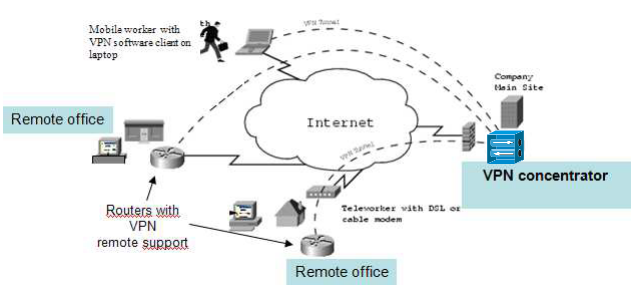
\includegraphics[scale=0.8]{figures/ex/VPN.png}
\caption{VPN IPSec}
\end{figure}
\end{center}

Risoluzione:

$S=0.01$. VPN IPSec. Accesso da remoto ad Internet e si basa sulla presenza di un \textit{VPN Concentrator} (concentratore di reti virtuali). IPSec, SSL. Meccanismi di sicurezza. Concentratore tramite VPN. Un router normale ne supporta fino ad una centinaia di VPN (Grandi aziende come CISCO, IBM). Le richieste di instaurazione arrivano secondo un processo di POISSON. $\lambda = 200\ req/h$. Inoltre $\frac{1}{\mu} = 30\ min$ (tempo medio di servizio). $m=?\ |\ \Pr\{LOSS\} < (S = 0.01)$.

M/M/m/0. Il processo degli arrivi di POISSON. Ci viene chiesto il numero di VPN contemporanee da supportare. Sistema con PERDITA (LOSS). ed ipotesi standard sui vari tempi. $m$ router. $m$ numero di VPN contemporanee. FCFS come disciplina di coda. Non c'è una coda però, quindi non conta tanto. $(\iff d=0, (e=+\infty))$.

Vogliamo utilizzare le tabelle (B di ERLANG). Il \underline{CARICO MEDIO di LAVORO} (INTENSIT\`A DI TRAFFICO) è $(\frac{\lambda}{\mu}) = (200 x 0.5) = 100 \implies (118=m)$. $S = 0.1$ (percentuale di perdita). [ERLANG] Sebbene sia in realtà una quantità adimensionata.

\newpage

\subsection{Sistemi a coda M/M/inf}

Sistema a coda costituito da un insieme illimitato di router. NON ABBIAMO FILA DI ATTESA! (Risorse illimitate). I clienti NON sono costretti a permanere in fila di attesa. Essa è quindi praticamente irrilevante. $N(t)$ al solito è il numero di clienti nel sistema a tempo $t$. Spazio degli stati di dimensione illimitata $\iff S=\{0,1,2,\ \dots\}$. Stesse ipotesi. $N(t)$  CATENA DI MARKOV a tempo continuo (CMTC), nascita e morte, con il seguente DTT:

\begin{center}
\begin{tikzpicture}[->, >=stealth', auto, semithick, node distance=2.3cm]
\tikzstyle{every state}=[fill=white,draw=black,thick,text=black,scale=0.8]
\node[state]    (0)                     {$0$};
\node[state]    (1)[right of=0]   {$1$};
\node[state]    (2)[right of=1]   {$2$};
\node[state] (d) [right of=2] {\ldots};
\node[state]    (im1)[right of=d]   {$i-1$};
\node[state]    (i)[right of=im1]   {$i$};
\node[state]    (ip1)[right of=i]   {$i+1$};
\node[state]    (ip2)[right of=ip1]  {$i+2$};
\node[state]    (d2)[right of=ip2]   {\ldots};
\path
(0) edge[bend left]     node{$\lambda$}         (1)
(1) edge[bend left]     node{$\lambda$}         (2)
    edge[bend left,below]    node{$\mu$}            (0)
(2) edge[bend left]     node{$\lambda$}           (d)
    edge[bend left,below]    node{$2\mu$}             (1)
(d) edge[bend left]         node{$\lambda$}   (im1)
	edge[bend left,below]   node{$3\mu$}          (2)
(im1) edge[bend left]       node{$\lambda$}  (i)
	  edge[bend left,below]   node{$(i-1)\mu$}     (d)
(i)   edge[bend left]   node{$\lambda$}      (ip1)
      edge[bend left,below]  node{$i\mu$}          (im1)
(ip1) edge[bend left]       node{$\lambda$}  (ip2)
	 edge[bend left,below]   node{$(i+1)\mu$}      (i)
(ip2)edge[bend left]       node{$\lambda$}  (d2)
	 edge[bend left,below]   node{$(i+2)\mu$}     (ip1)
(d2)edge[bend left,below]    node{$(i+3)\mu$}     (ip2);
\end{tikzpicture}
\end{center}

Abbiamo:

\[
	\left\{
	\begin{aligned}
	&\lambda_i=\lambda,\ i\geq 0\\
	&\mu_i=i\mu,\ i\geq 1
	\end{aligned}
	\right.
\]

Tassi di nascita $\lambda$, tassi di morte $i\mu$. Numero di stati illimitato. La CATENA è OMOGENEA, IRRIDUCIBILE. Dobbiamo vedere se è ERGODICA:

\[
	\left\{
	\begin{aligned}
	&[\pi_i = \pi_0 (\frac{\lambda}{\mu})^i \frac{1}{i!}]\\
	&[\pi_0 = \frac{1}{1+\sum_{k=1}^\infty{(\frac{\lambda}{\mu})^k \frac{1}{k!}}}]
	\end{aligned}
	\right.
\]

Anzitutto come sempre inglobiamo il termine 1 nella sommatoria dell'ultima equazione. Essa converge sempre. Abbiamo:

\[
	\pi_0 = \frac{1}{\sum_{k=0}^\infty{(\frac{\lambda}{\mu})^k \frac{1}{k!}}} = \e^{-\frac{\lambda}{\mu}}
\]

ove si è sfruttato il fatto che: $[\sum_{i=0}^\infty{x^i\frac{1}{i!}} = \e^x]$. Quindi NO CONDIZIONE DI ERGODICIT\`A. Tale serie CONVERGE SEMPRE. Converge sempre a patto che $\{\lambda,\mu\}$ siano finiti $(\iff \lambda,\mu <+\infty)$. Abbiamo:

\[
	\pi_i = \pi_0 (\frac{\lambda}{\mu})^i \frac{1}{i!} = (\frac{\lambda}{\mu})^i \frac{1}{i!}\e^{-\frac{\lambda}{\mu}},\ i\geq 0
\]

\underline{CATENA SEMPRE ERGODICA}. Non dobbiamo soddisfare nulla. Notiamo subito che riflette una DISTRIBUZIONE DI POISSON di parametro $\frac{\lambda}{\mu}$. Quindi: $[\bar{N} = (\frac{\lambda}{\mu})]$, anche se l'avrei potuto pure trovare con Little questo risultato: $\bar{N} = \lambda (\frac{1}{\mu})$. Quanto abbiamo detto vale per tempi di servizio distribuiti genericamente (\underline{\underline{M/G/$\infty$}}).
Tale sistema a coda è utilizzato per la modellazione dei tempi di propagazione. I tempi di propagazione sono considerati all'incirca costanti e pari a circa $(\sim \frac{2}{3} c)$.

%************************************************
% Chapter 3: AFFIDABILITA' E DISPONIBILITA'
%************************************************
% !TEX encoding = UTF-8
% !TEX TS-program = pdflatex
% !TEX root = ../nt.tex
% !TEX spellcheck = it-IT

%************************************************
\chapter{Affidabilità e Disponibilità}
\label{cap:relavl}
%************************************************\\

\section{Starting Point}

\subsection{Exercise}

CSP = \textit{Content Service Provider}. Abbiamo una batteria di $K$ server, tutti equivalenti. Server soggetti a guasti. $M$ server di backup. Quando un server si blocca viene sostituito con un server di backup, SE DISPONIBILE. Se i $K$ server funzionano tutti siamo in "\textit{Normal State}", Se inferiori a $K$ il sistema si blocca e siamo in "\textit{Failure State}". Ce ne devono essere almeno $K$.

\{TTF per il processo expneg. con parametro $f_p$, TTF memoria expneg. con parametro $f_m$, TTF disco expneg. con parametro $f_d$\}.

DTT, probabilità di regime, frazione di tempo Failure State, MTTF del sistema; durata media dell'intervallo di tempo tra un istante in cui il servizio è attivato e l'istante successivo corrispondente alla sospensione del servizio.

In totale ci sono $\underline{K+M}$ server (server attivi + server di backup). La situazione normale sarebbe il seguente tableau: $\{K,0,M\}$, ove i tre parametri indicano rispettivamente i server funzionanti della server farm, quelli in riparazione e quelli di backup. Ad un certo punto potrebbe accadere che nella server farm vi siano $K$ server ed $M$ in riparazione. Un ulteriore guasto della server farm porterebbe il sistema ad entrare in Failure State. Dinamica relativa al sistema. Definizione di Stato: processo stocastico: numero di server nella server farm e nei server di backup. Questa definizione di stato ci va bene per un processo Markoviano. Le tre v.a. sono indipendenti. Il tempo di guasto di un server sarà il minimo di queste tre v.a. dei TTF. Se quindi $f=f_p+f_m+f_d$, allora il tempo di guasto del server sarà tale che $TTF \sim EXP(f)$. I tempi di guasto dei vari server sono v.a. indipendenti. Le riparazioni procedono in parallelo tra di loro. Tempi di riparazione indipendenti dai tempi di guasto $\iff$ PROCESSO MARKOVIANO, il cui DTT è il seguente:

\begin{center}
\begin{tikzpicture}[->, >=stealth', auto, semithick, node distance=2cm]
\tikzstyle{every state}=[fill=white,draw=black,thick,text=black,scale=1]
\node[state]    (KPM)                     {$K+M$};
\node[state]    (KPMM1)[right of=KPM]   {$K+M-1$};
\node[state]    (KPMM2)[right of=KPMM1]   {$K+M-2$};
\node[state] (KPMM3) [right of=KPMM2] {$K+M-3$};
\node[state]    (d)[right of=KPMM3]   {\ldots};
\node[state]    (KP1)[right of=d]   {$K+1$};
\node[state]    (K)[right of=KP1]   {$K$};
\node[state]    (KM1)[right of=K]  {$K-1$};
\path
(KPM) edge[bend left]     node{$Kf$}         (KPMM1)
(KPMM1) edge[bend left]     node{$Kf$}         (KPMM2)
    edge[bend left,below]    node{$\mu$}            (KPM)
(KPMM2) edge[bend left]     node{$Kf$}           (KPMM3)
    edge[bend left,below]    node{$2\mu$}             (KPMM1)
(KPMM3) edge[bend left]         node{$Kf$}   (d)
	edge[bend left,below]   node{$3\mu$}          (KPMM2)
(d) edge[bend left]       node{$Kf$}  (KP1)
	  edge[bend left,below]   node{$4\mu$}     (KPMM3)
(KP1)   edge[bend left]   node{$Kf$}      (K)
      edge[bend left,below]  node{$(M-1)\mu$}          (d)
(K) edge[bend left]       node{$Kf$}  (KM1)
	 edge[bend left,below]   node{$M\mu$}      (KP1)
(KM1) edge[bend left,below]   node{$(M+1)\mu$}     (K);
\end{tikzpicture}
\end{center}

Il numero di stati è finito $(\iff \cardinality{stati}<+\infty)$. Si suppone che le riparazioni avvengano in parallelo, altrimenti se ci fosse una Single Repair Facility $\mu$ sarebbe costante. Quindi abbiamo: $N(t)=K+M$, ovvero $K$ server nella server farm che si possono guastare. Il tempo di guasto è dato da $\rightarrow$

\[
	\phi_{K+M}(t) = \underline{\min{(\dots)}}
\]

ove la parte sottolineata indica i tempi di guasto residui al tempo $t$. Se siamo nello stato $K$, vi sono $M$ \underline{in riparazione} e 0 nella stanza dei server di backup. Può accadere che ad un certo punto si guasti un ulteriore server della server farm $\implies$ FAILURE STATE. La velocità totale di uscita dallo stato $K+M$ sarebbe proprio $Kf$.

\begin{itemize}

\item{\textbf{NORMAL STATE}} fino a $K$;
\item{\textbf{FAILURE STATE}} $K-1$;
\end{itemize}

Oscillazione tra normal state e failure state. La seguente Catena di Markov vagherà tra questi stati. Non esiste una singola definizione di stato. Ce ne possono essere differenti. Alcune volte delle differenti definizioni di stato potrebbero portare allo stesso DTT. Considerando ad esempio $N(t)$ come il numero di server in riparazione avremo il seguente DTT:

\begin{center}
\begin{tikzpicture}[->, >=stealth', auto, semithick, node distance=2cm]
\tikzstyle{every state}=[fill=white,draw=black,thick,text=black,scale=1]
\node[state]    (0)                     {$0$};
\node[state]    (1)[right of=0]   {$1$};
\node[state]    (2)[right of=1]   {$2$};
\node[state] (3) [right of=2] {$3$};
\node[state]    (d)[right of=3]   {\ldots};
\node[state]    (MM1)[right of=d]   {$M-1$};
\node[state]    (M)[right of=MM1]   {$M$};
\node[state]    (MP1)[right of=M]  {$M+1$};
\path
(0) edge[bend left]     node{$Kf$}         (1)
(1) edge[bend left]     node{$Kf$}         (2)
    edge[bend left,below]    node{$\mu$}            (0)
(2) edge[bend left]     node{$Kf$}           (3)
    edge[bend left,below]    node{$2\mu$}             (1)
(3) edge[bend left]         node{$Kf$}   (d)
	edge[bend left,below]   node{$3\mu$}          (2)
(d) edge[bend left]       node{$Kf$}  (MM1)
	  edge[bend left,below]   node{$4\mu$}     (3)
(MM1)   edge[bend left]   node{$Kf$}      (M)
      edge[bend left,below]  node{$(M-1)\mu$}          (d)
(M) edge[bend left]       node{$Kf$}  (MP1)
	 edge[bend left,below]   node{$M\mu$}      (MM1)
(MP1) edge[bend left,below]   node{$(M+1)\mu$}     (M);
\end{tikzpicture}
\end{center}


ove cambierebbero solo le label rispetto al precedente.
Non è importante il modo in cui si chiamino gli stati, ma le loro transizioni! PROCESSO STOCASTICO: numero di server in riparazione al tempo $t$; CATENA ERGODICA (OMOGENEA, IRRIDUCIBILE con $\cardinality{stati}<+\infty$). In funzione della distribuzione di regime dobbiamo trovare altre quantità:

$\pi_{M+1}$ sarebbe la frazione di tempo a regime ove il servizio è sospeso, quindi $\underline{1-\pi_{M+1}} = \underline{\pi_0+\ \dots+\ \pi_M}$ sarebbe invece la frazione di tempo a regime nel quale il sistema si trova nello stato NORMAL, per via della condizione di NORMALIZZAZIONE. Il LHS è proprio la DISPONIBILIT\`A.

$\underline{1-\pi_{M+1}}$ AVAILABILITY del mio sistema di servizio. MTTF: durata (media) dell'intervallo che è costituito dall'istante di tempo di funzionamento alla sospensione. MTTF = \textit{Mean Time To Failure}. Rappresenta un processo stocastico, sebbene non markoviano, con stati: $S=\{ON,\ OFF\}$, ove ON sta per NORMAL ed OFF per FAILURE. Ad un certo punto la catena sarà in $M$. L'MTTF è la durata media dell'intervallo di tempo che va dall'inizio dello stato $M$ sino all'istante di Failure, ovvero un istante immediatamente prima delle sospensione del servizio. Invece MTTR significa \textit{Mean Time To Recovery}.

\begin{defn}{\textbf{AVAILABILITY}}

L'AVAILABILITY è la frazione del tempo in cui il sistema sta ad erogare il servizio:

\[	
	A := [\frac{MTTF}{MTTF+MTTR}]
\]

\end{defn}

Noi parleremo di ALTA DISPONIBILIT\`A. 5-9 ($99.999\%$), che rappresenta un downtime annuo di circa 5 minuti. Disponibilità molto alta in realtà bancarie. L'MTTR corrisponde al tempo medio di soggiorno della mia catena nello stato $M+1$. Il valor medio del tempo di soggiorno è $\frac{1}{(M+1)\mu}$. 

Consideriamo il seguente risultato:

\[
	MTTF = \frac{1}{(M+1)\mu\pi_{M+1}} - (\dots)
\]

dove $(\dots)$ rappresenta il tempo medio di soggiorno da sottrarre (durata media di quell'intervallo). Quindi:

\[
	MTTF = (\dots) = \frac{1}{(M+1)\mu\pi_{M+1}} - \frac{1}{(M+1)\mu} = \frac{1}{(M+1)\mu} \frac{1-\pi_{M+1}}{\pi_{M+1}} \implies
\]
\[
	\implies [\frac{MTTF}{\frac{1}{(M+1)\mu}} = \frac{1-\pi_{M+1}}{\pi_{M+1}}] \implies \frac{MTTF}{MTTR} = \frac{1-\pi_{M+1}}{\pi_{M+1}}
\]

Vale il BILANCIAMENTO LOCALE. Abbiamo che:

\begin{itemize}

\item{$\frac{1}{(M+1)\mu}$} è il tempo medio di soggiorno della mia catena nello stato $M+1$;
\item{$\frac{1}{(M+1)\mu\pi_{M+1}}$} è il tempo medio di ricorrenza (o di ritorno) nello stato $M+1$;
\end{itemize}

La differenza ci ritorna l'MTTF. Abbiamo sfruttato il fatto che la frequenza dell'evento ritorno nello stato di normal state è: $\pi_{M+1}(M+1)\mu$, mentre a titolo informativo la frequenza dell'evento ingresso nello stato di failure è $\pi_MKf$. Le due frequenze sono ovviamente uguali in virtù dell'applicazione dell'equazione di bilanciamento locale, dato che questa CMTC è di tipo Nascita e Morte.

Se si volesse utilizzare la tecnica degli stati assorbenti (vedasi \textbf{CMTC with Absorbing States}), allora bisognerebbe considerare come STATO ASSORBENTE \{M+1\}, e bisognerebbe tenere opportunamente in conto le condizioni iniziali del processo.

Sistemi di servizio che possono trovarsi in due stati: \{NORMAL STATE, FAILURE STATE\}, mappati rispettivamente in $SYS:\ \{ON,\ OFF\}$. Prendiamo in considerazione due sistemi:

\begin{itemize}

\item{\textit{Primo sistema}}: \newline
Tale sistema mediamente per $1s$ si trovi nello stato OFF, e per $9s$ nello stato ON. La disponibilità di questo sistema è: $A = \frac{9s}{10s} = 90\%$, ovvero per il $90\%$ del tempo il sistema è perfettamente funzionante, nello stato di ON.

\item{\textit{Secondo sistema}}: \newline
Tale sistema invece è UP per $0.9s$, e down per $0.1s$. Abbiamo sempre una disponibilità di $A = \frac{0.9s}{1s} = 90\%$, come il primo sistema;

\end{itemize}

La \underline{\underline{disponibilità}} è la medesima per i due sistemi, ma l'affidabilità invece è maggiore nel primo (non ha a che fare con il tempo di Recovery).


\begin{defn}{\textbf{AFFIDABILIT\`A}}

L'Affidabilità è formalmente definita come:

\[
	R(t) := \Pr\{X > t\} = Reliability(t)
\]
\end{defn}

Non sarebbe nient'altro che la CDF complementare della v.a. $X$, la quale rappresenta il tempo di vita del sistema. Non pensiamo alla riparazione o sostituzione. Si parte dall'affidabilità dei singoli componenti. Per l'analisi di affidabilità sono molto utili gli RBD, ovvero i \textit{Reliability Block Diagram}.

\subsection{Ridondanza}

Web server SW processo applicativo che si guasta con un failure rate $\gamma_p$. In esecuzione con una macchina che si guasta indipendentemente a failure rate $\gamma_m$. Il failure rate corrisponde ad un parametro della distribuzione esponenziale. Definizione di failure rate dipendente dal tempo. Vi è un meccanismo automatico di \textit{Failure Detection}, basato sul polling. Il tempo medio necessario per rilevare il failure sul server sia $\frac{1}{\delta_p}$ e che $\frac{1}{\delta_m}$ sia il tempo medio di rilevazione failure macchina.

Quando la macchina ha un malfunzionamento, il processo applicativo è migrato su una macchina di riserva, se \underline{DISPONIBILE}. $\frac{1}{\tau_m}$ è il tempo medio necessario per avviare la macchina di backup. Se invece si ha un guasto soltanto del processo server, viene automaticamente riavviato sulla stessa macchina. Il tempo medio di restart del server software è $\frac{1}{\tau_p}$. Tipicamente $[\tau_p > \tau_m] \implies \frac{1}{\tau_p} < \frac{1}{\tau_m}$. C'è una piccola probabilità $(1-c)$ che il restart del processo sulla stessa macchina non vada a buon fine, nel qual caso è avviato sulla macchina di riserva. Questo schema di (re)start automatico dopo i guasti è anche chiamato "\textit{cold replication}". Quando una macchina crasha, è necessario un recovery più complesso dal relativo rate $\mu$. Il Web server è considerato disponibile quando sia il processo server che la macchina sulla quale esso gira sono entrambi funzionanti. Si valuti la \textit{Steady-State Availability} del server, assumendo che non vi siano ulteriori guasti del processo o della macchina fino a che non siano stati adeguatamente trattati (risolti).

Quindi la DISPONIBILIT\`A viene meno quando nè il processo nè la macchina sono funzionanti. AFFIDABILIT\`A di un sistema cold-replicated $\implies$ RIDONDANZA. RIDONDANZA o \textit{REPLICATION ATTIVA} quando vi sono oltre ai server operativi anche dei server di backup, tutti quanti soggetti alla stessa quantità di lavoro (in tal caso anche quelli di backup lavorano come quelli normali). Si suppone che il failure rate sia il medesimo per entrambi i tipi. Il contrario è la REPLICATION PASSIVA $\rightarrow$ \{WARM REPLICATION, COLD REPLICATION\}. Si immagini di avere due server, due macchine. Uno attivo è l'altro di backup. Con la WARM, di tanto in tanto quello di backup interagisce con quello attivo per ricevere le sue strutture dati. Un malfunzionamento di quello attivo fa sì che si attivi quello di backup. Ma il relativo tempo del recovery è molto basso. Ci piace questo, però a trasferire queste strutture dati periodicamente, una parte delle capacità elaborative sarà riservata a questa mansione. Potrebbe invece eseguire altri jobs al posto di questi. Vantaggi in tempi di Recovery, però il problema è legato ad un throughput più basso del server attivo. Con quella a freddo abbiamo un tempo di recovery più alto, ma sull'attivo sfruttiamo perlomeno tutta la capacità elaborativa. Parametri: \{performance, affidabilità della rete (dei vari dispositivi di cui la rete si compone)\ (\textit{reliability R(t), fault tolerance}), Sicurezza dati\}. L'esercizio in questione propone la ridondanza di un Server. Potrebbero esserci dei \textit{WATCH-DOG}, ovvero dei "cani da guardia" che controllano il server primario. Controllo delle eventuali degradazioni delle prestazioni in un cluster - Policing, disciplina decidibile.

Studiamo il sistema con un approccio Markoviano. DTT della CMTC che modella il sistema. Faremo l'ipotesi di distribuzione esponenziale per le v.a. in gioco (Anche per la distribuzione relativa al Failure Detection Time).

\[
	\left\{
	\begin{aligned}
	&F_p \sim EXP(\gamma_p),\ F_m \sim EXP(\gamma_m)\\
	&D_p \sim EXP(\delta_p),\ D_m \sim EXP(\delta_m) \\
	&R_p \sim EXP(\tau_p),\ R_m \sim EXP(\tau_m)
	\end{aligned}
	\right.
\]

Rispettivamente, le prime due equazioni della prima riga indicano la distribuzione dei time to failure di un processo o della macchina, le successive due della seconda riga indicano la distribuzione dei time to failure detection del processo o della macchina, e le ultime due della terza riga indicano la distribuzione del time to (re)start del processo \underline{sulla stessa macchina} (SAME MACHINE) o del riavvio del processo sulla macchina di riserva (SPARE MACHINE). $(1-c)$ rappresenta invece la probabilità che il riavvio del processo sulla stessa macchina fallisca. Quindi $c$ è il \textit{coverage factor}, ovvero la probabilità di successo del riavvio del processo. Infine abbiamo: $C_r \sim EXP(\mu)$, ovvero il tempo di riparazione per una macchina andata in crash (crashed machine recovery). Il DTT è il seguente:

\begin{center}
\begin{tikzpicture}[->, >=stealth', auto, semithick, node distance=3cm]
\tikzstyle{every state}=[fill=white,draw=black,thick,text=black,scale=1]
\node[state]    (01X1)                     {$01X1$};
\node[state]    (11X1)[above right of=01X1]   {$11X1$};
\node[state] (0D1X1) [right of=01X1] {$0D1X1$};
\node[state]    (X0DX1)[below of=01X1]   {$X0DX1$};
\node[state]    (11X0D)[right of=11X1]   {$11X0D$};
\node[state]    (11X0)[below of=11X0D]   {$11X0$};
\node[state]    (0D1X0)[right of=11X0D]   {$0D1X0$};
\node[state]    (01X0)[right of=0D1X0]  {$01X0$};
\node[state]    (F)[below of=01X0]  {$F$};
\node[state]    (X0X1)[below left of=F]  {$X0X1$};
\path
(11X1) edge[bend left]     node{$\gamma_m$}         (11X0D)
       edge[right]   node{$\gamma_m$}   (X0DX1)
       edge[bend left,above]     node{$\gamma_p$}   (0D1X1)
(01X1) edge[bend left]     node{$c\tau_p$}         (11X1)
    edge[bend right]    node{$tau_p(1-c)$}            (X0X1)
(0D1X1) edge[bend right,above left]     node{$\delta_p$}           (01X1)
(X0DX1) edge[bend right]         node{$\delta_m$}   (X0X1)
(X0X1) edge[bend left,right]        node{$\tau_m$} (11X0)
(11X0D) edge[bend left]       node{$\delta_m$}  (11X0)
(0D1X0)   edge[bend left]   node{$\delta_p$}      (01X0)
(01X0) edge[bend left]       node{$c\tau_p$}  (11X0)
	 edge[bend left]   node{$c(1-\tau_p)$}      (F)
(F) edge[bend left]   node{$\mu$}     (X0X1)
(11X0) edge[bend right] node{$\gamma_p$} (0D1X0)
 edge[bend right] node{$\gamma_m$} (F)
 edge[bend right] node{$\mu$} (11X1);
\end{tikzpicture}
\end{center}

La definizione di stato si basa sui seguenti stati degli elementi \{(Processo primario, Macchina primaria), (Processo secondario, Macchina secondaria)\}, riassumibili nel seguente apposito tableau:

\[
	\begin{bmatrix}
	P_p&P_m\\S_p&S_m
	\end{bmatrix}
\]

Tale è la rappresentazione del DTT di una CMTC che modella un Web Server con Cold Replication con una macchina di backup. $\{P_p,\ P_m\}$ rappresentano rispettivamente gli stati del processo primario e della macchina primaria sulla quale questo processo è in esecuzione. I pedici $\{p,m\}$ si riferiscono rispettivamente al processo od alla macchina. Gli altri due indici, $\{S_p,\ S_m\}$ stanno per SPARE o secondary. E stanno per lo stato del processo server di backup e della relativa macchina sulla quale esso sta in esecuzione, al solito. $P \rightarrow primary,\ S \rightarrow spare$. $"1" \rightarrow$ processo/macchina up; $"0" \rightarrow"$ processo/macchina down. Se $P_p=1\ \lor P_m=1 \implies$ il processo/macchina primario/a è up. $P_p=0\ \lor\ P_m=0 \implies$ processo/macchina primaria down. Vale anche per gli altri ovviamente. $"0D" \rightarrow$ processo/macchina è failed (guasta), con malfunzionamento, ma il rispettivo guasto non è ancora stato rilevato (To be detected). $"X" \rightarrow$ don't care. Valori possibili. Possiamo pensare di partire dallo stato: \{1,1,X,1\} $\implies P_p=P_m=1$. (processo e macchina primaria entrambi UP). Macchina secondaria funzionante e non ci interessa del processo secondario. Ai fini delle transizioni di stato, ci può essere un malfunzionamento o del processo primario, o della macchina primaria od ancora quella di backup. $\gamma_p$ è il parametro della distribuzione esponenziale che modella il TTF del processo. Supponiamo si sia verificato un malfunzionamento del processo primario. Macchina primaria/secondaria entrambe UP $\rightarrow 0D=P_p \rightarrow P_p=0$. Altra transizione. Macchine ancora entrambe UP. Dopo che il sistema di Failure Detection avrà fatto per l'appunto detection del failure, a velocità $\delta_p$, lo stato sarà: \{0,1,X,1\}. A questo punto si tenta di riavviare il processo (come accade tipicamente nei SO) sulla stessa macchina. Abbiamo un Coverage Factor pari a $c$, ovvero pari alla probabilità che il riavvio vada a buon fine. $(1-c)$ è per contro, la probabilità che vada male il riavvio. Se il riavvio sulla stessa macchina ha successo, migriamo conseguentemente verso lo stato iniziale \{1,1,X,1\} a velocità $c\tau_p$. Altrimenti con velocità $(1-c)\tau_p$ migriamo verso lo stato \{X,0,X,1\}. Siamo in situazione di macchina primaria Down. Con certezza la macchina per me è in crash. Macchina inutilizzabile. Siamo quindi in \{X,0,X,1\}. Macchina 1 in crash. Bisogna quindi cambiare macchina. $\tau_p$ è il parametro che caratterizza la distribuzione esponenziale relativa al restart time della macchina stessa. Consideriamo la v.a. tempo di soggiorno residuo nello stato: \{0,1,X,1\}, di indice 4. $\phi_4 \sim EXP(\mathord{\cdot})$. Consideriamo:

\[
	\Pr\{\phi_4(t) > \tau\} = \Pr\{R_{Rp} > \tau\} = \e^{-\tau_p\tau}
\]

dove $R_{Rp}$ rappresenta il restart time del processo (residuo), e tale è la probabilità che esso sia maggiore di $\tau$. Indica quanto manca ancora affinché il restart finisca. $R_{Rp}$ sarà distribuita proprio come il Restart Time del processo sulla macchina attiva. $R_p$ è il restart time, mentre $R_{Rp}$ è il restart time residuo. Nell'istante $t$ stiamo quindi in questo stato. Questo restart potrebbe andar bene od andar male. Velocità totale di uscita banalmente $\tau_p$. Quindi:

\[
	\tau_{i,j} = \frac{q_{i,j}}{-q_{ii}} = \tau_{4,1} = \frac{q_{4,1}}{-q_{4,4}} = \frac{q_{4,1}}{\tau_p} \implies
\]
\[
	\implies \tau_{4,1} = c \implies q_{4,1}=c\tau_p
\]

La macchina è andata in crash, a questo punto. Bisogna quindi cambiare macchina. Ci vuole un altro tempo che indichiamo con $R_m$, ovvero il restart time del processo sulla macchina secondaria. Con velocità $\tau_m$ arriveremo da \{X,0,X,1\} $\rightarrow$ \{1,1,X,0\} (Non ho più una macchina di riserva). Quella primaria si è sostanzialmente scambiata con la secondaria (funzionante). A velocità $\mu$ dopodiché, avremo la riparazione e migriamo verso lo stato iniziale, nuovamente: \{1,1,X,1\}. Possono accadere però altre cose. Dobbiamo anche considerare che, o accada un malfunzionamento della macchina primaria o della secondaria. \{1,1,X,1\} $\rightarrow$ \{X,0D,X,1\} $\rightarrow$ \{X,0,X,1\} a velocità $\delta_m$, quest'ultimo passaggio. Poi arriveremo verso \{1,1,X,0\} ad avvenuta sostituzione. $\gamma_m$ è il parametro che caratterizza la distribuzione esponenziale della $F_m$, ovvero il TTF della macchina. Sempre $\gamma_m$ per la failure. Partiamo da \{1,1,X,0\}. NO macchina secondaria a disposizione. O malfunzionamento del processo primario o della macchina secondaria. Se accade un malfunzionamento del processo primario, migrerò con velocità $\gamma_p$ verso \{0D,1,X,0\}, ed a velocità $\delta_p$ verso \{0,1,X,0\}. Se si verifica un failure della macchina andremo in FAILURE direttamente a velocità $(1-c)\tau_p$. Ma se a partire da \{1,1,X,0\} si guasta completamente la macchina, allora migreremo direttamente in \textbf{FAILURE} totale a velocità $\gamma_m$. Notiamo che siamo in situazione di SRF (\textit{Single Repair Facility}).

Studio di fattibilità. Non è importante l'etichetta che attribuiamo agli stati quanto il loro significato. A questo punto li etichettiamo. Procedura di Labelizing. Distribuzioni di regime. Sistema di 10 equazioni (9 eq. + 1 eq. normalizzazione). Sfruttiamo la conoscenza del valore dei diversi parametri in gioco.
Si valuti quindi la Steady-State Availability del Server. Stati nei quali il Web Server funziona. Gli stati dove $P_p=1$ sono:

\[
	\left\{ \begin{bmatrix}1&1\\X&1\end{bmatrix},\ \begin{bmatrix}1&1\\X&0\end{bmatrix},\ \begin{bmatrix}1&1\\X&0D\end{bmatrix} \right\}
\]

A questo punto, abbiamo che: $[A = \pi_1 + \pi_6 + \pi_7]$, secondo la nuova notazione indiciale rappresentata nella seguente maniera, nella notazione \textit{State name} $\rightarrow$ \textit{State index}:

\begin{itemize}
\item{\{1,1,X,1\}} $\rightarrow$ 1;
\item{\{0D,1,X,1\}} $\rightarrow$ 2;
\item{\{X,0D,X,1\}} $\rightarrow$ 3;
\item{\{0,1,X,1\}} $\rightarrow$ 4;
\item{\{X,0,X,1\}} $\rightarrow$ 5;
\item{\{1,1,X,0D\}} $\rightarrow$ 6;
\item{\{1,1,X,0\}} $\rightarrow$ 7;
\item{\{0D,1,X,0\}} $\rightarrow$ 8;
\item{\{0,1,X,0\}} $\rightarrow$ 9
\item{\{1,1,X,1\}} $\rightarrow$ 10;

\end{itemize}

\[
	\left\{
	\begin{aligned}
	&\frac{1}{\gamma_p} = 10\ days, \frac{1}{\gamma_m} = 20\ days\\
	&\frac{1}{\delta_p} = 1 s, \frac{1}{\delta_m} = 0.4/0.5 s\\
	&\frac{1}{\tau_m} = 2\ min, \frac{1}{\tau_p} = 30s
	\end{aligned}
	\right.
\]

\[
	\left\{
	\begin{aligned}
	&\pi_1 = \frac{1}{E},\ \pi_2 = \frac{1}{E} \frac{\gamma_p}{\delta_p},\ \pi_3 = \frac{1}{E} \frac{\gamma_m}{\delta_m},\ \pi_4 = \frac{1}{E} \frac{\gamma_p}{\tau_p}\\
	&\pi_5 = \frac{1}{E} \frac{[\gamma_m + (1-c)\tau_p][\mu + 2\gamma_m + (1-c)\tau_p]}{\mu\tau_m}\\
	&\pi_6 = \frac{1}{E} \frac{\gamma_m}{\delta_m},\ \pi_7 = \frac{1}{E} \frac{2\gamma_m + (1-c)\gamma_p}{\mu}\\
	&\pi_8 = \frac{1}{E} [2\gamma_m + (1-c)\gamma_p]\gamma_p,\ \pi_9 = \frac{1}{E} \frac{[2\gamma_m + (1-c)\gamma_p]\gamma_p}{\mu\tau_p}\\
	&\pi_{10} = \frac{1}{E} \frac{[2\gamma_m + (1-c)\gamma_p][\gamma_m + (1-c)\gamma_p]}{\mu^2}
	\end{aligned}
	\right.
\]

dove:

\[
	E = 1 + \frac{\gamma_p}{\delta_p} + 2\frac{\gamma_m}{\delta_m} + \frac{\gamma_p}{\delta_p} + \frac{[\gamma_m + (1-c)\gamma_p][\mu+2\gamma_m + (1-c)\gamma_p]}{\mu\tau_m} +
\]
\[
	+ \frac{2\gamma_m + (1-c)\gamma_p}{\mu} [1+\frac{\gamma_p}{\delta_p} + \frac{\gamma_p}{\tau_p}] + \frac{[2\gamma_m + (1-c)\gamma_p][\gamma_m + (1-c)\gamma_p]}{\mu^2}
\]

ed otteniamo alla fine:

\[
	A = \pi_1 + \pi_6 + \pi_7 = \frac{1}{E} [1+\frac{\gamma_p}{\delta_p} + \frac{2\gamma_m + (1-c)\gamma_p}{\mu}]
\]

Abbiamo così trovato la Steady-State Availability $A$.

\section{Affidabilità}

\{\underline{Affidabilità}, \underline{Disponibilità}\}. Come può esser valutata l'Affidabilità di un Sistema. Affidabilità di un Dispositivo / servizio di Rete. Concetti legati ma differenti.

Reliability $R(t)$. Affidabilità. Indipendentemente dalla rete / servizi di rete. L'Affidabilità può esser applicata dappertutto. L'Affidabilità va PROGETTATA. \underline{Reliability Engineering}. Di mezzo ci sono queste tecniche, che si servono principalmente dei \newline \underline{diagrammi a blocchi dell'affidabilità}, detti RBD. Utilizzo delle CATENE DI MARKOV. Dato $\mathit{S}$ un sistema, componente, apparato, switch lvl 2 o lvl 3, l'affidabilità esprime la capacità, relativamente a quel sistema, di funzionare correttamente per un certo periodo di tempo. $X$ è il time to failure del sistema (lifetime del sistema). Indichiamo con $f(t)$ la PDF di $X$, ovvero la densità di probabilità. Sia invece $F(t)$ la CDF di $X$ (funzione di distribuzione cumulativa). L'Affidabilità $R(t)$ è definita come:

\begin{defn}{\textbf{Affidabilità}}

\[
	R(t) := \Pr\{X > t\} = 1-F(t) = F^c(t)
\]

\end{defn}

Non è nient'altro che la CDF complementare, ed indica la probabilità che il TTF sia maggiore di un certo tempo $t$, non meglio definito per il momento
Probabilità che $\mathit{S}$ sia funzionante correttamente in $[0,t)$. $\Pr\{\mathit{S}\ correctly\ working\ in\ [0,t)\}$. Tempo di vita almeno pari a $t$, ovvero che $\mathit{S}$ sopravviva per almeno $t$ unità di tempo. Normalmente si suppone che il sistema lavori correttamente nell'istante iniziale, ovvero $\iff R(0)=1$ (con probabilità unitaria il lifetime sia maggiore di 0). Potrebbe anche accadere che in alcuni casi $\Pr\{X=0\} = p\neq 0$ (che un dispositivo NON funzioni all'inizio). Normalmente si ha invece: $\Pr\{X=0\} = (0=p)$. Tipicamente quindi $R(0)=1$. Poi si suppone che: $[\lim_{t\to+\infty}{R(t)} = 0] \iff$ un sistema NON possa funzionare indefinitamente. Inizialmente funzioni correttamente e prima o poi si guasterà. Sostanzialmente, graficamente parlando, $\Pr\{X > t\}$ rappresenta l'area sottesa dalla relativa PDF $f(t)$ in $[t,+\infty)$. $R(t)$ è la CDF complementare di $X$, quindi vale:

\[
	\left\{
	\begin{aligned}
	&[R(t) = \int_t^{+\infty}{f(x)dx}]\\
	&[R'(t) = -\frac{d F(t)}{dt} = -f(t)]
	\end{aligned}
	\right.
\]

Ovvero che la derivata dell'affidabilità, $R'(t)$, non è nientemeno che la PDF del TTF $X$ o lifetime cambiata di segno. 

Qual'è invece il MTTF? Valor medio del time to failure? (tempo medio di vita):

\[
	MTTF = \E[X] = \int_0^\infty{tf(t)dt} = \int_0^\infty{R(t)dt}
\]

ovvero che il MTTF è sostanzialmente l'integrale dell'affidabilità. Si dimostra integrando per parti.

\[
	\underline{\E[X]} = \int_0^{+\infty}{[1-F(t)]dt} - \int_{-\infty}^0{F(t)dt}
\]

L'integrazione per parti dimostra ciò. Questo vale generalmente quando $\E[X] \leq\geq 0$. Ma se il lifetime è maggiore di 0, come nel nostro caso, dal momento che è una variabile aleatoria soltanto a valori positivi (v.a. positiva), allora banalmente vale che: 

\[
	\int_{-\infty}^0{F(t)dt} = 0 \implies \E[X] = \int_0^{+\infty}{[1-F(t)]dt} = \int_0^\infty{\underline{R(t)}dt}
\]

ovvero che il MTTF è l'integrale dell'affidabilità, come già detto. Ricordiamo che MTTF sarebbe il \textit{Mean Time To Failure}, ed il MTBF significa \textit{Mean Time Between Failure}. Sono sostanzialmente la stessa cosa ma nominate in modo diverso. A volte nei paper della CISCO si preferisce utilizzare il MTBF. I valori possono tranquillamente raggiungere 40 anni. Esistono metodi di calcolo che favoriscono il confronto (Metodi Standard).  

Definiamo il: FAILURE RATE (istantaneo). (Instantaneous) Failure Rate. Partiamo dalla PDF della v.a. $X$ TTF o lifetime:

\[
	f(t) = \frac{d F(t)}{dt} = \lim_{\Delta t\to 0}{[\frac{F(t+\Delta t)-F(t)}{\Delta t}]}
\]

A numeratore abbiamo: $\Pr\{t < X \leq t+\Delta t\}$, per $\Delta t$ sufficientemente piccolo. Per $\Delta t\to 0$, abbiamo che $f(t)\Delta t$ rappresenta la probabilità che il tempo di vita di quella v.a. vari tra $t$ e $t+\Delta t$. Per $\Delta t\to 0$ il prodotto $f(t)\Delta t \to \Pr\{t < X \leq t+\Delta t\}$. Questa è una probabilità NON condizionata. Adesso consideriamo: $\Pr\{t < X \leq t+\Delta t\ |\ X > t\} = (\dots)$, che sarebbe la probabilità che, dato che il sistema è sopravvissuto per $t$ unità di tempo, non sopravviva per ulteriori $\Delta t$ unità di tempo. Abbiamo che:

\[
	(\dots) = \frac{\Pr\{t < X \leq t+\Delta t,\ X > t\}}{\Pr\{X > t\}} = [\frac{\Pr\{t < X \leq t+\Delta t\}}{\Pr\{X > t\}}] \implies
\]

ove si è sfruttato il seguente fatto:

\[
	\{X > t\} \subset \{t < X \leq t+\Delta t\} \implies \Pr\{t < X \leq t\Delta t \cap X > t\} = \Pr\{t < X \leq t+\Delta t\}
\]

A denominatore abbiamo l'Affidabilità $R(t)$. Definiamo ora l'IFT $h(t)$ come:

\begin{defn}{\textbf{(Instantaneous) Failure Rate}}

L'IFT (\textit{Instantaneous Failure Rate}) è definito come:

\[
	h(t) := \lim_{\Delta t \to 0}{[\frac{1}{\Delta t} \frac{\Pr\{t < X \leq t+\Delta t\}}{R(t)}]} = \mathord{\cdot}(t)
\]

\end{defn}

Questa è la definizione del Failure Rate istantaneo. $\Delta t\to 0 \implies h(t)\Delta t$ rappresenta la probabilità che, supponendo che il dispositivo sia sopravvissuto per $t$ unità di tempo, non sopravviva per ulteriori $\Delta t$ unità di tempo. Ma notiamo che:

\[
	h(t) = \lim_{\Delta t\to 0}{\frac{1}{\Delta t} \frac{F(t+\Delta t)-F(t)}{R(t)}} = \frac{f(t)}{R(t)}
\]

ovvero corrisponde al rapporto tra la PDF e la CDF complementare della v.a. $X$. Sappiamo inoltre che: $f(t)=-R'(t) \implies$

\[	
	h(t) = -\frac{(R'(t) = -f(t))}{R(t)} = \frac{-R'(t)}{R(t)}
\]

Ma essendo l'affidabilità una probabilità $\implies R(t) \in [0,1]$. Quindi ne consegue che: $h(t)\geq f(t)$. Ma a questo punto, indipendentemente da $\Delta t\to 0$, abbiamo che: $[h(t)\Delta t\geq f(t)\Delta t]$. Vero indipendentemente dal valore di $\Delta t$. Quindi, ricapitolando, $f(t)\Delta t$ rappresenta la probabilità che il tempo di vita sia compreso tra $t$ e $t+\Delta t$, mentre $h(t)\Delta t$ indica la probabilità che, sapendo che il dispositivo sia sopravvissuto sino a $t$, muoia nei prossimi $\Delta t$. $h(t)$ è quindi sensibilmente più grande di $f(t)$, indipendentemente da $\Delta t$. 

Ci serve un modo teorico per ricavare questi valori. Abbiamo tre macro-fasi di vita del dispositivo, sintetizzabili in un grafico di $h(t)$ in funzione del tempo $t$. Abbiamo un andamento cosiddetto a \textit{CURVA di VASCA DA BAGNO}. Abbiamo la prima fase di mortalità infantile, che include l'avvenimento di eventuali difetti di fabbrica, quindi $h(t)$ è alto. Poi abbiamo la seconda fase, ove $h(t)$ è tipicamente basso, ovvero il ciclo di vita utile del dispositivo. Qualunque malfunzionamento qui deriva da PROBLEMI ESOGENI, ove lo stress è dovuto a cause esterne. Poi abbiamo un'ultima fase di senilità, ove comprensibilmente $h(t)$ torna ad esser nuovamente alto in quanto vi è l'USURA del dispositivo da tener in conto. $h(t)=\frac{f(t)}{R(t)}=\frac{-R'(t)}{R(t)}$ rappresenta quindi la velocità alla quale un sistema tende a rompersi.

Il Failure Rate NON è un qualcosa di costante, ma varia con il tempo! Nel calcolo pratico si ipotizza sempre che siamo nella seconda fase di vita del dispositivo, ovvero quella di vita utile.

I seguenti elementi: $\{MTTF=\E[X],\ R(t),\ h(t)\}$ sono in stretta relazione tra di loro. Sia $N_0$ il numero di dispositivi messi ad operare tutti insieme nell'istante $(t_0=0)$. Siano nelle stesse condizioni di lavoro di partenza. Per tutti INIZIA il tempo di vita. Same working conditions. Al generico istante $t$, possiamo osservare lo stato di questi dispositivi. $N_S(t)$ sia il numero di dispositivi SURVIVED (sopravvissuti), per i quali il tempo di vita NON è terminato. Vale: $N_F(t) = \underline{N_0-N_S(t)} \implies [N_S(t) + N_F(t) = N_0]$ (popolazione iniziale). Se dovessi vedere come varia questa funzione $N_S(t)$ al variare del tempo, avrei una funzione a gradino decrescente. I guasti, ovvero le variazioni del grafico, avvengono in istanti $t_i$. L'intervallo $[0,t_1]$ comprende il tempo di vita del primo dispositivo che si è guastato, e così via... Set di dati corrispondenti ai TTF dei vari dispositivi. Mediando (aritmeticamente), otteniamo: 

\[
	\underline{\hat{\E}[X]} = \frac{t_1+t_2 +\ \dots+\ t_{N_0}}{N_0} = \frac{1}{N_0}\sum_{i=0}^{N_0}{t_i}
\]

Sarebbe la media empirica dei tempi di guasto. Se $N_0\to+\infty$, quella media empirica tende all'$\E[X]$. Con una popolazione sufficientemente grande, $\hat{\E[X]} \to \E[X]$. Abbiamo una BUONA STIMA procedendo in questo modo. \`E richiesto un numero sufficientemente grande di dispositivi iniziali. Come stimiamo invece l'Affidabilità? $\iff \hat{R}(t)=?$ Si immagini che $X \sim EXP(\lambda)$. A questo punto abbiamo:

\[
	h(t) = \frac{-R'(t)}{R(t)} = \frac{f(t)}{R(t)} = \frac{\lambda\e^{-\lambda t}}{\e^{-\lambda t}} = \lambda (\neq \mathord{\cdot}(t))
\]

Quindi abbiamo un IFR $h(t)$ costante e pari a $\lambda$ quando $X \sim EXP(\lambda)$. Calcoliamo $\E[X]$:

\[
	MTTF = \E[X] = \int_0^\infty{R(t)dt} = \frac{1}{\lambda}\int_0^\infty{\lambda\e^{-\lambda t}dt} = (\frac{1}{\lambda})*1
\]

Se la distribuzione del TTF è esponenziale, $\lambda=h(t)$ ed $(\frac{1}{\lambda})$ è il suo valore medio. TTF è ovviamente il lifetime. $\E[X]$ è l'inverso del FAILURE RATE in tal caso, che è costante.

Tipicamente il TTF di una macchina potrebbe avere come parametro: $[f = f_p+f_m+f_d]$. In tal caso:

\[
	\left\{
	\begin{aligned}
	&f = f_p+f_m+f_d\\
	&X \sim EXP(f)\\
	&R(t) = \e^{-ft}
	\end{aligned}
	\right.
\]

Diamo una definizione:

\begin{defn}{\textbf{funzione di affidabilità EMPIRICA}}

\[
	\hat{R}(t) = \frac{N_S(t)}{N_0}
\]

\end{defn}

\`E chiaro che se $N_0\to +\infty \implies \hat{R}(t) \to R(t)$.

\begin{defn}{\textbf{failure rate empirico}}

\[
	\hat{h}(t) = -(\frac{1}{\Delta t})\frac{[\hat{R}(t+\Delta t) - \hat{R}(t)]}{\hat{R}(t)}
\]

\end{defn}

Al solito, $N_0\to +\infty \implies \hat{h}(t)\to h(t)$.

\section{Disponibilità}

\begin{defn}{\textbf{Disponibilità}}

Si definisce formalmente la DISPONIBILIT\`A ISTANTANEA:

\[
	\underline{A(t)} := \Pr\{in\ t\ il\ dispositivo\ sia\ UP\}
\]

\end{defn}

Inizieremo dalla DISPONIBILIT\`A ISTANTANEA, per poi passare dalla DISPONIBILIT\`A IN UN INTERVALLO sino ad arrivare alla DISPONIBILIT\`A A REGIME.

AVAILABILITY = DISPONIBILIT\`A. Dobbiamo pensare alla riparazione/sostituzione di un componente del dispositivo. \textit{Instantaneous Availability} $A(t)$, probabilità che un sistema stia funzionando correttamente al tempo $t$. Questo indipendentemente dal numero di guasti o riparazioni che possano essere avvenuti prima di $t$. Consideriamo la v.a. $I(t)$ indicatrice:

\[
	I(t) := \left\{
	\begin{aligned}
	&1,\ sistema\ UP\\
	&0,\ sistema\ DOWN
	\end{aligned}
	\right.
\]

\`E un indicatore dello stato del sistema. Il valor medio di $I(t)$, per un noto lemma, è:

\[
	\underline{A(t)} = \Pr\{I(t) = 1\} = \underline{\E[I(t)]}
\]

$I(t)$ è una v.a. binaria $\iff$ può assumere solo valori 0 e 1. Pensiamo ad una singola realizzazione di $I(t)$. Indichiamo con $x_i$ la durata dell'i-esimo periodo di up e con $D_i$ la durata dell'i-esimo periodo di down $\iff \{x_i,D_i\} \rightarrow \{UP,\ DOWN\}$. Definiamo la:

\begin{defn}{\textbf{Interval Availability}}

\[
	\bar{A}(t) := \underline{\frac{1}{t}\int_0^t{A(x)dx}}
\]
\end{defn}

Somiglia molto ad una media temporale. Questa quantità è la frazione di tempo nella quale il sistema è UP limitatamente alla finestra temporale $[0,t]$. 

\[
	\bar{A}(t) = \frac{1}{t}\int_0^t{\E[I(x)]dx} = \frac{1}{t}\underline{\E[\int_0^t{I(x)dx}]}
\]

Ove l'ultima uguaglianza deriva per linearità, ed il termine sottolineato è il \newline \underline{\textit{Mean Total Uptime}} (MTU). Questo integrale ha a che fare con il total Uptime in $[0,t]$, ovvero limitatamente a quell'intervallo: $\int_0^t{I(x)dx}$. Questa quantità sarà alla fine uguale all'MTTF.

Definiamo:

\begin{defn}{\textbf{STEADY-STATE AVAILABILITY}}

\[
	A := \lim_{t\to +\infty}{\bar{A}(t)}
\]
\end{defn}

ovvero il limite dell'Interval Availability. Ricordiamo che MTTF, MTTR significano rispettivamente: \textit{Mean Time To Failure} e \textit{Mean Time To Recovery/Repair}, sebbene per l'ultimo acronimo si preferisca la terminologia \textit{Recovery}, perché si preferisce includere anche i tempi di Detection e di sopralluogo. 

Una formula che troviamo in letteratura è:

\[
	[A = \frac{MTTF}{MTTF+MTTR}]
\]

ove $A$ rappresenta la frazione del tempo ove il sistema è UP, ovvero la durata media del ciclo UP-DOWN. Sta erogando il servizio per il quale è stato pensato. Troviamo in realtà anche questa formula:

\[
	A = \underline{\frac{MTBF}{MTBF+MTTR}}
\]

Se abbiamo sistemi che una volta guasti vengono riparati e sostituiti. Si utilizzano in realtà entrambe le notazioni. Quindi $MTBF=MTTF$, non c'è nessuna differenza. Si utilizza l'$MTTF$ quando NON abbiamo possibilità di riparazione.

\[
	A = \frac{durata\ media\ periodo\ UP}{durata\ media\ periodo\ UP+durata\ media\ periodo\ DOWN} = \frac{MTTF}{MTTF+MTTR}
\]

Esistono dei grandi numeri per la $MTBF$, ovvero la Mean Time Between Failure. Ma in realtà NON è realistico avere un dispositivo che funzioni per 40 anni. Ma se tutti i produttori adottassero lo stesso procedimento, allora le quantità sarebbero perlomeno confrontabili. Per vedere la durata realistica si dovrebbe procedere assumendo un numero elevato di componenti e fare la media aritmetica dei tempi di guasto. Valutazione dell'Affidabilità di un Sistema a partire dall'Affidabilità dei singoli componenti. Se tutti questi attuassero questa procedura alla stessa maniera, i valori sarebbero però confrontabili. Se volessimo una valutazione realistica dell'Affidabilità di un Sistema, dovremmo ovviamente partire da Affidabilità Realistiche dei singoli componenti. Per alcuni componenti si sanno i valori realistici. Nella realtà non abbiamo il ragionevole tempo di osservare $N_0$, con $(N_0\to +\infty)\uparrow$. Popolazione iniziale eccessivamente elevata.

Tipicamente il Failure Rate di un sistema (funzione che varia nel tempo, $h(t)$), è costante $\impliedby$ se la distribuzione della v.a. $X$ è esponenziale. 
Avremo un andamento che segue abbastanza bene il profilo di una vasca da bagno.

La curva suggerisce l'esistenza di tre fasi: \textit{Mortalità Infantile}, \textit{Useful Life} e \textit{Wearout Phase} Nella fase di Mortalità Infantile, come suggerisce lo stesso nome, i Failure sono dovuti a prolbemi ENDOGENI. Eventuali progettazioni non fatte bene. All'inizio abbiamo un Failure Rate abbastanza elevato. Poi abbiamo la vita utile e poi di nuovo dei valori alti nella wearout phase (dovuti tipicamente all'usura). Se la prima fase è superata, possiamo sempre andare incontro a failure, ma nella Useful Life essi sono dovuti a problemi ESOGENI (Cause di stress per un dispositivo).

Nella Useful Life il Failure Rate del dispositivo è costante; questo fatto corrisponde ad un'ipotesi. Durante la Vita Utile sono le condizioni di Stress che provocano malfunzionamenti. Di tanto in tanto lo stress raggiunge dei picchi, oltrepassando lo Stress Max che il dispositivo può tollerare. Situazioni di stress (particolari) $\implies$ il dispositivo va incontro a malfunzionamenti. Se $\lambda$ è il Failure Rate, è auspicabile pensare che lo stress sia un processo di POISSON (a velocità $\lambda$). $N_t := \cardinality{picchi\ in\ [0,t]}$. Se il processo dei picchi è di POISSON abbiamo:

\[
	[\Pr\{N(t) = \underline{k}\} = \frac{(\lambda t)^k}{k!}\e^{-\lambda t}]
\]

POISSON, con $[k\geq 0]$. Quando il failure rate è costante $\iff$ la v.a. $X$ è distribuita esponenzialmente con parametro $\lambda$. Si consideri la probabilità che $\Pr\{X > t\}$, ovvero l'\underline{AFFIDABILIT\`A}. La probabilità che $X > t$, che il tempo di vita del dispositivo sia maggiore di $t$, è UGUALE alla probabilità che fino a $t$ non ci siano stati picchi:

\[
	\implies (\dots) = \Pr\{N_t = 0\} = \e^{-\lambda t}
\]

(la distribuzione è esponenziale). Se il failure rate è costante, la distribuzione del lifetime è esponenziale. Superata la fase Useful Life abbiamo la fase del LOGORIO, quando il dispsositivo comincia ad usurarsi. Se NON ci fosse quest'usura, la durata media dell'Intervallo di Useful Life sarebbe realisticamente molto grande.

\{MTTF, =MTBF\} $\leftarrow$ quando si valutano queste quantità si suppone sempre di stare in Useful Life. Valori grandi. 

\section{RBD (Reliability Block Diagram)}

\underline{Reliability Block Diagram}, ovvero diagrammi a blocchi dell'Affidabilità. Strumento teorico per valutare l'Affidabilità di un sistema a partire dall'Affidabilità degli elementi di cui esso si compone. Per tirare fuori gli RBD dobbiamo partizionare un sistema in elementi con specifici task. Parliamo di un sistema con \textit{STRUTTURA SEMPLICE} per riferirci ad un sistema che può essere modellato mediante un RBD costituito da blocchi combinati secondo strutture \{SERIE, PARALLELO, $k$-out-of-$n$ ("k su n")\}, ed in cui i vari blocchi sono indipendenti l'uno dall'altro. I blocchi modellano l'Affidabilità dei componenti. L'Affidabilità è: $\Pr\{X > t\}$. Blocchi indipendenti $\implies$ elementi indipendenti $\implies$ tempi di guasto v.a. indipendenti. Il tempo di guasto in un certo blocco non va ad influire sui tempi di guasto degli altri, e dualmente, non è influenzato dai tempi di guasto di un altro blocco.

\subsection{Struttura SERIE}

Due blocchi in serie. Con il rettangolo tratteggiato stiamo considerando il sistema costituito dai blocchi in serie:

\begin{center}
\begin{figure}[H]
\centering
\includegraphics[scale=0.7]{figures/relavl/series.png}
\caption{Struttura Serie}
\end{figure}
\end{center}

Siano: $\{R_1(t),\ R_2(t)\}$ le rispettive due Affidabilità degli elementi $\{E_1,E_2\}$, due elementi di un sistema, ai quali corrispondono due blocchi di Affidabilità in serie. L'intero sottosistema funziona bene se i due sotto-elementi funzionano. Ogni elemento della struttura serie deve funzionare. \textit{PATH} che porta dall'Ingresso all'Uscita. Se un elemento NON funziona è come se nel mezzo ci siano circuiti aperti. Se un elemento è guasto, è considerato come \textit{CIRCUITO APERTO}. Sia $X$ il time to failure dell'intero sottosistema, $X_1$ il lifetime associato ad $E_1$ ed $X_2$, diametralmente, sia il lifetime associato ad $E_2$. Abbiamo: 

\[
	R_{series}(t) = \Pr\{X > t\} = \Pr\{X_1 > t,\ X_2 > t\} = \Pr\{X_1 > t\}\Pr\{X_2 > t\} = \underline{R_1(t)R_2(t)}
\]

ove si è sfruttato l'indipendenza dei blocchi per scrivere la probabilità dell'evento INTERSECT $\iff$ la probabilità congiunta è il PRODOTTO delle probabilità. Il termine sottolineato è quindi il prodotto delle due Affidabilità. Possiamo naturalmente generalizzare, scrivendo che:

\begin{thrm}{\textbf{Affidabilità sottosistema SERIE}}

L'Affidabilità di un sottosistema serie costiuito da $n$ componenti è:

\[
	R_{series}(t) := \prod_{i=1}^n{R_i(t)}
\]

\end{thrm}

Questa è anche detta \underline{Product law of Reliability}. Ad esempio se abbiamo 5 componenti in serie (elementi) tali per cui:

\[
	R_i(t) = R = 0.970\ \forall i=1,2,\dots,5 \implies R_{series} = (0.97)^5 = 0.859
\]

Se ne avessimo 10 con questa stessa Affidabilità dei singoli componenti, avremmo invece $R_{series}=(0.97)^{10} = 0.738$. Si supponga ora di avere un sistema costituito da: \{HARD DISK, PROCESSORE, MEMORIA\}, rispettivamente mappati nell'RBD come: $\{E_1,E_2,E_3\}$. Sia $X \sim EXP(f)$, dove $\underline{f = f_p + f_{mem} + f_{HD}}$. Allora l'Affidabilità del computer è: $[R(t) = \e^{-ft},\ f = f_p+f_{mem}+f_{HD}]$. 
Procedendo con gli RBD, troviamo:

\[
	\left\{
	\begin{aligned}
	&R_{proc}(t) = \e^{-f_pt}\\
	&R_{mem}(t) = \e^{-f_{mem}t}\\
	&R_{HD}(t) = \e^{-f_{HD}t}
	\end{aligned}
	\right.
\]

Facendo il prodotto abbiamo:

\[
	R_{series}(t) = R_{proc}(t)R_{mem}(t)R_{HD}(t) = \e^{-(f_p+f_{mem}+f_{HD})t} = \e^{-f_pt}\e^{-f_{mem}t}\e^{-f_{HD}t}
\]

I vari elementi combinati in serie devono quindi funzionare, e DEVONO funzionare molto bene per un'alta affidabilità. Quindi, se consideriamo due elementi in serie abbiamo che: $R(t) = R_1(t)R_2(t)$. Se consideriamo:

\[
	\left\{
	\begin{aligned}
	&R'(t) = R_1'(t)R_2(t) + R_1(t)R_2'(t)\\
	&\left[
	\begin{aligned}
	h_{series}(t) &= \frac{-R'(t)}{R(t)} = -\frac{R_1'(t)R_2(t)}{(R(t)=R_1(t)R_2(t))} -\frac{R_1(t)R_2'(t)}{R_1(t)R_2(t)} =\\
	&= -\frac{R_1'(t)}{R_1(t)}-\frac{R_2'(t)}{R_2(t)} = h_1(t)+h_2(t) = \sum_{i=1}^2{h_i(t)}
	\end{aligned}
	\right.
	\end{aligned}
	\right.
\]

Generalizzando abbiamo che:

\begin{thrm}{\textbf{Failure Rate sottosistema SERIE}}

Il Failure Rate di un sottosistema serie costiuito da $n$ componenti è:

\[
	h_{series}(t) = \sum_{i=1}^n{h_i(t)}
\]

\end{thrm}

in generale considerando $n$ elementi. Il failure rate totale corrispondente è la sommatoria dei vari failure rati associati ai singoli elementi. Abbiamo: \{Prodotto delle $R_i(t)$, sommatoria degli $h_i(t)$\}.

\subsection{Struttura PARALLELO}

\begin{center}
\begin{figure}[H]
\centering
\includegraphics[scale=0.7]{figures/relavl/parallel.png}
\caption{Struttura Parallelo}
\end{figure}
\end{center}

Siano sempre: $\{R_1(t)\rightarrow E_1(t),\ R_2(t)\rightarrow E_2(t)\}$. Valutiamo l'Affidabilità del sistema parallelo. Il sistema funziona se ALMENO uno degli elementi funziona.

\[
	R_{parallel}(t) = \Pr\{X > t\} = 1-\Pr\{X\leq t\} = 1-\Pr\{X_1\leq t,\ X_2\leq t\} = (\dots)
\]

Dato che parliamo di blocchi indipendenti abbiamo: $\implies \Pr\{X > t\} = 1-\Pr\{X_1\leq t\}\Pr\{X_2\leq t\}$. Quindi:

\[
	(\dots) = 1-(1-\underline{(\Pr\{X_1 > t\} = R_1(t))})(1-\underline{(\Pr\{X_2 > t\} = R_2(t))}) =
\]
\[
	= 1-\prod_{i=1}^2{(UNRELIABILITY)_i}
\]

Ove i termini sottolineati sono le due affidabilità, $R_1(t),R_2(t)$. Si può notare una definizione alternativa, eseguendo i prodotti opportuni:

\[
	(\dots) = [\underline{\Pr\{X_2>t\} + \Pr\{X_1>t\} - \Pr\{X_1>t\}\Pr\{X_2>t\}}]
\]

Formalizziamo:

\begin{thrm}{\textbf{Affidabilità sottosistema PARALLELO}}

L'Affidabilità di un sottosistema parallelo costiuito da $n$ componenti è:

\[
	R_{parallel}(t) := 1-\prod_{i=1}^n{(1-R_i(t))}
\]

\end{thrm}

Si potrebbe in realtà fornire una definizione alternativa sfruttando il \textit{principio di inclusione-esclusione}, od il teorema della probabilità totale.

Esempio con singole affidabilità uguali a quelle del precedente esempio: $R_{parallel}(t) = 1-(1-0.97)^2 = 0.9991$, con due componenti. Mettendo 5 componenti in parallelo invece troviamo: $R_{parallel}(t)=1-(1-0.97)^5=0.9999999757$, ovvero un'altissima affidabilità. RIDONDANZA. Elementi RIDONDANTI. Struttura RIDONDANTE. I blocchi in tal caso sono in parallelo.

Per quanto concerne il failure rate, supponiamo di avere due dispositivi in parallelo, con parametri indipendenti tra di loro. L'Affidabilità complessiva è:

\[	
	R(t) = R_2(t)+R_1(t)-R_1(t)R_2(t)
\]

Calcoliamo quindi il failure rate, omettendo la dipendenza funzionale temporale onde alleggerire la notazione $\iff R_i:=R_i(t),\ i=1,2$:

\[
	h_{parallel}(t) = -\frac{R'(t)}{R(t)} =
\]
\[
	= -\frac{R_2'}{R_2+R_1-R_1R_2} -\frac{R_1'}{R_2+R_1-R_1R_2} +\frac{R_1'R_2}{R_2+R_1-R_1R_2} +\frac{R_1R_2'}{R_2+R_1-R_1R_2} =
\]
\[
	= -\frac{R_1'}{R_2+R_1-R_1R_2}[1-R_2] -\frac{R_2'}{R_2+R_1-R_1R_2}[1-R_1]
\]

Di per sé non ha un particolare significato esplicito. Se ci restringiamo al caso in cui abbiamo dispositivi identici, con quindi la stessa affidabilità $(\iff R_1=R_2:=R)$, otteniamo invece:

\[
	h_p := h_{parallel}(t) = -\frac{R'}{2R-R^2} -\frac{R'}{2R-R^2} = -2\frac{R'(1-R)}{R(2-R)} = -2h\frac{(1-R)}{2-R}
\]

Ancora una volta, sarebbe possibile formalizzare il tutto sfruttando il teorema della probabilità totale.
	

\subsection{Struttura k-out-of-n}

\begin{center}
\begin{figure}[H]
\centering
\includegraphics[scale=0.7]{figures/relavl/KoutofN.png}
\caption{Struttura Parallelo}
\end{figure}
\end{center}

Sia l'Affidabilità $= (\mathord{\cdot}(t))$, ovvero stiamo sempre pensando ad un certo tempo. L'intero sistema funziona solo se ALMENO $k$ su $n$ elementi funzionano. Sistema UP quando ci sono $k$ server funzionanti, ad esempio. Supponiamo per semplicità (wlog) che le Affidabilità dei vari elementi siano uguali: $[R_i(t)=R_e(t)]\ \forall i=1,2,\dots,n$. Abbiamo:

\[
	R_{k/n}(t) = \Pr\{"almeno\ k\ elementi\ sopravvivono\ fino\ al\ tempo\ t"\} = \Pr\{X > t\} =
\]
\[
	= \Pr\{\cup_{i=k}^n{["i\ elementi\ sopravvivono\ fino\ al\ tempo\ t,\ exactly"]}\} = (\dots)
\]

Ma gli eventi in gioco sono DISGIUNTI! $\implies$

\[
	(\dots) = \sum_{i=k}^n{\Pr\{"exactly\ i\ elements\ survive\ until\ time\ t\}}
\]

Questa non è nient'altro che una sequenza di $n$ trial di Bernoulli indipendenti, quindi una \underline{DISTRIBUZIONE BINOMIALE}. Definiamo quindi:

\begin{defn}{\textbf{Affidabilità sottosistema k-out-of-n}}

L'Affidabilità di un sottosistema k-out-of-n costiuito da $n$ componenti è:

\[
	R_{k/n}(t) := \Pr\{X > t\} = \sum_{i=k}^n{\binom{n}{i}R_e(t)^i[1-R_e(t)]^{n-i}}
\]

\end{defn}

Bernoulli Trials. Ne si considerino tutte le $\binom{n}{i}$ combinazioni possibili di configurazioni ove almeno $k$ sono funzionanti. 

\subsubsection{Workstation and File Servers (Exercise)}

Consider a network service based on a system that consists of n workstations and m file servers. The network connecting these devices is assumed to be fault-free. The system is considered to be operational so long as at least k workstations and l file servers are operational. Let $R_w(t)$ denote the reliability of a single workstation and Rf(t) the reliability of a single file server. Assuming that all devices fail independently of each other, evaluate system reliability. 

\begin{center}
\begin{figure}[H]
\centering
\includegraphics[scale=1]{figures/ex/ws&fs.png}
\caption{Workstations \& File Servers}
\end{figure}
\end{center}

Si supponga di avere $n$ workstation ed $m$ File Server. La rete che connette questi dispositivi è ad Affidabilità Unitaria (\textit{Fault-Free}). Il sistema è considerato essere operativo quando almeno $k$ workstation ed $l$ file server sono operativi. I due macrosistemi sono ovviamente collegati in serie. Abbiamo il seguente RBD:

\begin{center}
\begin{figure}[H]
\centering
\includegraphics[scale=0.7]{figures/relavl/sysrel.png}
\caption{Workstation \& File Servers RBD}
\end{figure}
\end{center}

Dunque risolviamo:

\[
	[R(t) = (\sum_{i=k}^n{\binom{n}{i}R_w(t)^i[1-R_w(t)]^{n-i}})(\sum_{i=l}^m{\binom{m}{i}R_f(t)^i[1-R_f(t)]^{m-i}})]
\]

\subsection{Network Lecce-Torino (Exercise)}

Consider the network in the figure below:

\begin{center}
\begin{figure}[H]
\centering
\includegraphics[scale=0.8]{figures/ex/nLT.png}
\caption{Network Lecce-Torino}
\end{figure}
\end{center}

Let $R_L(t)$ denote the reliability of links and assume that routers are fault-free. Evaluate the 
reliability of the path from Lecce to Torino. 
Possible routes for packets:  

\begin{itemize}

\item R1 - R4 - R5;
\item R1 - R3 - R5;
\item R1 - R2 - R3 - R5;

\end{itemize}

Risoluzione:

Network Lecce-Torino. $R_L(t)$ rappresenta l'affidabilità dei Link. Router fault-tree. Possibili rotte: $\{R_1-R_4-R_5,\ R_1-R_3-R_5,\ R_1-R_2-R_3-R_5\}$. Si enuncino i casi limite della struttura k-out-of-n:

\[
	\left\{
	\begin{aligned}
	&R_{1/n} = R_{parallel}(t)\\
	&R_{n/n} = R_{series}(t)
	\end{aligned}
	\right.
\]

Ipotesi fault-free. Router ridondati. Affidabilità talmente elevata da ritenersi unitaria, quindi fault-free. Si consideri quindi solo l'Affidabilità dei Link. Sistema semplice modellabile con blocchi in serie, in parallelo o k/n. I link avranno in realtà diverse affidabilità a seconda della lunghezza etc. Modelliamo questo sistema reale con un RBD, andando a considerare l'Affidabilità dei singoli link. Non modelliamo il link d'ingresso, ma volendo potremmo anche associargli un RB apposito (\textit{Reliability Block}). Facciamo un'IPOTESI IMPORTANTE: [\underline{Blocchi indipendenti}]. Modello RBD che modella l'Affidabilità di questa rete. L'RBD è il seguente:

\begin{center}
\begin{figure}[H]
\centering
\includegraphics[scale=0.7]{figures/relavl/nLT.png}
\caption{Network Lecce-Torino RBD}
\end{figure}
\end{center}

Sistema a struttura semplice, ovvero modellabile con blocchi di affidabilità combinati secondo strutture serie, parallelo, o k/n. Poniamo: $R_L(t) := (R\neq constant) = \mathord{\cdot}(t)$. Stiamo considerando la stessa affidabilità per tutti i link. Se avessimo blocchi ripetuti, essi non saranno assolutamente indipendenti! Rappresentiamo lo stesso elemento. Concetto di riduzione del modello iniziale in un modello a struttura semplice.

\[
	R_{collegamento}(t) = 1-(1-R^2)[1-R[1-(1-R)(1-R^2)]]
\]

Approccio di calcolo ricorsivo Top-Down. Elementi relativi ai blocchi. Ci sono delle tabelle con dei valori caratteristici.

\subsubsection{Network Lecce-Torino with Key-Item Method}

Consideriamo un esercizio con diagrammi con struttura NON semplice. Sempre Network Lecce-Torino. Reti fisiche. Router IP. Reti fisiche come dei link. Reti fisiche collegati da router IP. Si denoti con $R_L(t)$ l'Affidabilità dei Link. Due router IP collegati alla medesima rete fisica sono detti \underline{ADIACENTI}. Possibili rotte: $\{R_1-R_3-R_4,\ R_1-R_3-R_2-R_4,\ R_1-R_2-R_4,\ R_1-R_2-R_3-R_4\}$. Ci sono dei blocchi ripetuti fondamentalmente.

Consider the network in the figure below. 

\begin{center}
\begin{figure}[H]
\centering
\includegraphics[scale=0.8]{figures/ex/nLTKI.png}
\caption{Network Lecce-Torino \#Key-Item}
\end{figure}
\end{center}

Let $R_L(t)$ denote the reliability of links and assume that routers are fault-free. Evaluate the 
reliability of the path from Lecce to Torino. 
Possible routes for packets: 

\begin{itemize}

\item R1-R3-R4;
\item R1-R3-R2-R4;
\item R1-R2-R4;
\item R1-R2-R3-R4.

\end{itemize}

Risoluzione:

Consideriamo il relativo RBD:

\begin{center}
\begin{figure}[H]
\centering
\includegraphics[scale=0.6]{figures/relavl/nLTKI.png}
\caption{Network Lecce-Torino with Key-Item Method RBD}
\end{figure}
\end{center}

Il sistema è riducibile. L'RBD risultante potrebbe essere rappresentato anche nel seguente modo:

\begin{center}
\begin{figure}[H]
\centering
\includegraphics[scale=0.7]{figures/relavl/nLTKI2.png}
\caption{Network Lecce-Torino with Key-Item Method Reduced RBD}
\end{figure}
\end{center}

Sistema NON con struttura semplice, sebbene abbiamo dei blocchi indipendenti. Si sfrutti il \textit{Metodo Key-Item}, ovvero il Key-Item Method, in letteratura. Sostanzialmente si basa sul teorema delle probabilità totali. Condizionare rispetto allo stato di funzionamento dell'elemento chiave in gioco. Consideriamo quindi un elemento chiave $E_i(t)$ (\underline{$E_i$ is the key element}). 

\[
	R_S(t) = \Pr\{\underline{\mathit{S}\ sia\ UP\ in\ [0,t]}\} =
\]
\[
	= \Pr\{\mathit{S}\ sia\ UP\ in\ [0,t]\ |\ E_i\ sia\ UP\ in\ [0,t]\}(\Pr\{E_i\ sia\ UP\ in\ [0,t]\}=R_i(t)) +
\]
\[
	+ \Pr\{\mathit{S}\ sia\ UP\ in\ [0,t]\ |\ E_i\ sia\ DOWN\ in\ [0,t]\}(\Pr\{E_i\ sia\ DOWN\ in\ [0,t]\}=(1-R_i(t)))
\]

$\Pr\{X > t\}$ è la probabilità il componente sopravviva sino a $t$. Notiamo che:

\[
	\left\{
	\begin{aligned}
	&[\Pr\{E_i\ sia\ UP\ in\ [0,t]\}=R_i(t)]\\
	&[\Pr\{E_i\ sia\ DOWN\ in\ [0,t]\}=(1-R_i(t))]
	\end{aligned}
	\right.
\]

Se funziona sempre in $[0,t] \implies E_i$ diviene un CORTOCIRCUITO, diversamente nel secondo caso otteniamo un CIRCUITO APERTO. Potrebbe talvolta essere necessario applicare iterativamente il teorema delle probabilità totali sul nuovo scenario ottenuto. 

\[
	\left\{
	\begin{aligned}
	&\Pr\{\mathit{S}\ sia\ UP\ in\ [0,t]\ |\ E_i\ sia\ UP\ in\ [0,t]\}\rightarrow E_i\ \  CORTOCIRCUITO\\
	&\Pr\{\mathit{S}\ sia\ UP\ in\ [0,t]\ |\ E_i\ sia\ DOWN\ in\ [0,t]\}\rightarrow E_i\ \ CIRCUITO\ APERTO
	\end{aligned}
	\right.
\]

Ove le notazioni a destra si riferiscono al comportamento da schematizzare nel conseguente RBD. 

\begin{itemize}

\item{$E_i$ UP}: $\rightarrow R_a(t)$;
\item{$E_i$ DOWN}: $\rightarrow R_b(t)$
\end{itemize}

$\implies [R_s(t) = R_a(t)R_i(t) + R_b(t)(1-R_i(t))]$. Si considerino due casi quindi, entrambi da risolvere con la tecnica degli RBD, e laddove necessario si applichi ricorsivamente il TPT.

$L_{2-3}$ è nel nostro caso un candidato $E_i$:

\begin{itemize}

\item{a)} link 2-3 UP in $[0,t]$;
\item{b)} link 2-3 DOWN in $[0,t]$
\end{itemize}

Dobbiamo prima considerare il caso a, poi il caso b. Se lo CORTOCIRCUITO, il risultante RBD sarà la serie di due blocchi parallelo: $R_s = [1-(1-R)^2]^2$. Nel secondo caso invece otteniamo che dobbiamo rendere l'elemento chiave un CIRCUITO APERTO $\implies$ conseguente RBD semplice costituito dal parallelo di due serie $\implies R_s = [1-(1-R^2)^2]$. Quindi alla fine l'Affidabilità della PATH da Lecce a Torino è:

\[
	R_{path}(t) = R_a(t)R_{L_{2-3}}(t) + R_b(t)[1-R_{L_{2-3}}(t)]
\]

Nel caso il link chiave fosse unidirezionale, si potrebbe procedere in un solo verso. In tal caso avremmo sempre una struttura non semplice, ma in tal caso sarebbe consigliabile scegliere come elemento chiave $L_{3-4}$:
Adesso abbiamo quindi considerato cosa significa Affidabilità di un collegamento.

\subsection{SYSTEM RELIABILITY}

\begin{center}
\begin{figure}[H]
\centering
\includegraphics[scale=0.7]{figures/relavl/sysrel.png}
\caption{Workstation \& File Servers RBD}
\end{figure}
\end{center}

Supponiamo che dalle distribuzioni empiriche risulti che i TTF (time to failure) siano distribuiti esponenzialmente, rispettivamente:

\[
	\left\{
	\begin{aligned}
	&W_S \sim EXP(\lambda_W)\\
	&F_S \sim EXP(\lambda_f)
	\end{aligned}
	\right.
\]

$\{\lambda_W,\lambda_f\}$. Determiniamo l'Affidabilità del sistema ed il MTTF. Caso semplice: $n=2\ \land\ m=1\ \land\ k=l=1$. Riduzione a:

\[
	R_i(t) = R_f(t)[1-(1-R_w(t))^2] = \e^{-\lambda_ft}[1-(1-\e^{-\lambda_Wt})^2] = (\dots)
\]

dove abbiamo: $\{R_f(t)=\e^{-\lambda_ft},\ R_W(t)=\e^{-\lambda_Wt}\}$. Quindi:

\[
	(\dots) = \e^{-\lambda_ft}[1-(1+\e^{-2\lambda_Wt}-2\e^{-\lambda_Wt})] = \e^{-\lambda_ft}[2\e^{-\lambda_Wt} - \e^{-2\lambda_Wt}] =
\]
\[
	= [2\e^{-(\lambda_f+\lambda_W)t} - \e^{-(\lambda_f+2\lambda_W)t}]
\]

Questa è l'Affidabilità del sistema. Adesso abbiamo esplicitato la distribuzione di probabilità dell'Affidabilità. Il failure rate è: $\rightarrow$

\[
	[h(t) = \frac{-R'(t)}{R(t)}]
\]

Inoltre,

\[
	MTTF = \E[X] = \int_0^\infty{R(t)dt} = \int_0^\infty{(2\e^{-(\lambda_f+\lambda_W)t} - \e^{-(\lambda_f+2\lambda_W)t})dt} =
\]
\[
	= 2\int_0^\infty{\e^{-(\lambda_f+\lambda_W)t}dt} -\int_0^\infty{\e^{-(\lambda_f+2\lambda_W)t}dt} = \frac{2}{\lambda_f+\lambda_W}-\frac{1}{\lambda_f+2\lambda_W}
\]

Quanto detto per l'Affidabilità può anche esser esteso per la Disponibilità con gli ABD (\textit{Availability Block Diagram}), a patto che \underline{ttf} e \underline{ttr} siano v.a. indipendenti tra di loro $\implies \nexists$ Single Repair Facility (SRF) $\implies \forall$ elemento $\exists!$ Repair Facility. Altrimenti i vari ttr sarebbero dipendenti mutuamente. Se invece il sistema ha abbastanza risorse per le riparazioni degli elementi $\implies$ ttr v.a. indipendenti.

\subsection{ABD (Availability Block Diagram)}

Abbiamo:

\[
	\left\{
	\begin{aligned}
	&A_s(t) = \prod_{i=1}^n{A_i(t)},\ serie\\
	&A_p(t) = 1-\prod_{i=1}^n{(1-A_i(t))},\ parallelo
	\end{aligned}
	\right.
\]

Vale per Disponibilità istantanea, disponibilità in un intervallo e disponibilità a regime (che sarebbe il limite per $t\to +\infty$ della disponibilità in un intervallo). Supponendo $n=2,\ m=2,\ l=k=1$, si calcoli la Disponibilità del Sistema, supponendo che il $MTTF$ di una workstation sia $MTTF_W$ e quella del File Server sia $MTTF_f$. Analogamente per $MTTR_W,\ MTTR_f$. Si calcoli la disponibilità a regime, sfruttando i diagrammi a blocchi della disponibilità. 

La STEADY-STATE AVAILABILITY è:

\[
	A_{SS} = A_f[1-(1-A_w)^2]
\]

ma $A_f,A_w = ? \implies$

\[
	\left\{
	\begin{aligned}
	&A_f = \frac{MTTF_f}{MTTF_f+MTTR_R}\\
	&A_W = \frac{MTTF_W}{MTTF_W+MTTR_W}
	\end{aligned}
	\right.
\]

Il tempo di Restore include anche il tempo di rilevazione del malfunzionamento e di sopralluogo, oltre a quello ovviamente dell'effettiva riparazione.

\section{CMTC e Affidabilità}

CMTC, Catene di Markov a Tempo Continuo per il calcolo dell'Affidabilità. Catene di Markov con \textit{Stati ASSORBENTI}. Il sistema reale potrebbe ovviamente essere più complesso. Un servizio di Rete è basato su un sistema ridondante parallelo con 2 dispositivi. Il sistema è FALLITO quando entrambi i dispositivi sono guasti. Assumiamo: 

\[
	\left\{
	\begin{aligned}
	&TTF \sim EXP(\lambda)\\
	&TTR \sim EXP(\mu)
	\end{aligned}
	\right.
\]

$MTTF=?\ R(t)=?$. Interazioni più complesse che NON ci consentono di procedere con i normali RBD. Qui non solo i ttr NON sono indipendenti $\iff$ Single Repair Facility, ma è proprio l'interazione NON descrivibile mediante RBD.

\subsection{Stati Assorbenti}

PROCESSO STOCASTICO $N(t)=\cardinality{\{dispositivi\ funzionanti\ al\ tempo\ t\}}$. Devo calcolare l'Affidabilità del Sistema di servizio (dell'intero servizio). Questa servirà poi per il calcolo dell'$MTTF=\E[X]$. Voglio studiare questo sistema con un processo stocastico, il quale è una CMTC, il cui DTT è il seguente:

\begin{center}
\begin{tikzpicture}[->, >=stealth', auto, semithick, node distance=3cm]
\tikzstyle{every state}=[fill=white,draw=black,thick,text=black,scale=2]
\node[state]    (2)                     {$2$};
\node[state]    (1)[right of=2]   {$1$};
\node[state]    (0)[right of=1]   {$0$};
\path
(2) edge[bend left]     node{$2\lambda$}         (1)
(1) edge[bend left]     node{$\lambda$}         (0)
    edge[bend left,below]    node{$\mu$}            (2)
(0) edge[bend left,below]    node{$\mu$}             (1);
\node at ($(0)+(0,-1.5)$) {FAILED};
\end{tikzpicture}
\end{center}

I ttf sono tali per cui $ttf \sim EXP(\lambda)$, mentre il ttr è tale per cui $ttr \sim EXP(\mu)$. Abbiamo $S=\{0,1,2\}$ come spazio degli stati. Lo stato 0 rapresenta il fatto che non vi sono dispositivi funzionanti (stato FAILED). Ma qui contempliamo anche la possibilità che da FAILURE si torni nello stato UP. Possiamo anche considerare la DISPONIBILIT\`A.

\[
	\{\pi_2,\ \pi_1,\ \pi_0\} \implies A = \pi_2+\pi_1
\]

(quando il sistema sarà nello stato di NORMAL). Ma dobbiamo ora calcolare l'Affidabilità e l'MTTF. Computational Model. Modello di calcolo. Modello che si utilizza per calcolare una certa quantità. \{Affidabilità, MTTF\}. Modello di calcolo a partire dal modello di disponibilità (AVAILABILITY MODEL). La DTT diventa, a fronte di un opportuno detach del ramo di transizione che porta dallo stato di failure a normal:

\begin{center}
\begin{tikzpicture}[->, >=stealth', auto, semithick, node distance=3cm]
\tikzstyle{every state}=[fill=white,draw=black,thick,text=black,scale=2]
\node[state]    (2)                     {$2$};
\node[state]    (1)[right of=2]   {$1$};
\node[state]    (0)[right of=1]   {$0$};
\path
(2) edge[bend left]     node{$2\lambda$}         (1)
(1) edge[bend left]     node{$\lambda$}         (0)
    edge[bend left,below]    node{$\mu$}            (2);
\node at ($(0)+(0,-1.5)$) {FAILED};
\end{tikzpicture}
\end{center}

Sostanzialmente per quello che ci serve calcolare, partiamo dall'AM e facciamo un detach del ramo di transizione 0-1. $X,\ \Pr\{X > t\}$ è la nostra Affidabilità. Il sistema entra in FAIL quando si ha un ingresso nello stato 0 (Transizione 1-0), ovvero nello stato ASSORBENTE. \`E finito in tal caso il tempo di vita. Supponiamo che il sistema EVOLVA con due dispositivi funzionanti (evolva a partire dallo stato 2) $\implies$

\[
	\left\{
	\begin{aligned}
	&\pi_2(0)=1\\
	&\pi_1(0)=\pi_0(0)=0
	\end{aligned}
	\right.
\] 

Il ttf $X$ corrisponde al \textit{time-to-absorption} (il tempo per entrare nello stato assorbente) $\iff$ (TEMPO DI VITA = TEMPO DI ASSORBIMENTO). Cosicché $MTTF=MTTA$. Tutti gli altri stati sono stati TRANSITORI ($\nexists$ NON ESISTE distribuzione di regime). Ora mi servo di distribuzioni transitorie:

\[	
	\underline{\Pr\{X > t\}} = 1-\underline{\Pr\{X\leq t\}} = 1-\underline{\pi_0(t)}
\]

ove la probabilità $\pi_0(t)$ corrisponde alla probabilità che prima di $t$ si sia entrati nello stato assorbente. Abbiamo $X=ttf=tta$. C'è un solo stato assorbente, ve ne sono due transitori e quindi $\implies \nexists \pi_i=\lim_{t\to +\infty}{\pi(t)}$. 

\[
	[\frac{d \pi_i(t)}{dt} = \sum_{j\in S}{q_{ji}\pi_j(t)},\ \forall i\in S]
\]

Potremmo utilizzare queste equazioni ed applicarle a questa catena. In particolare, agli stati $\{0,1,2\}$. Abbbiamo:

\[
	\left\{
	\begin{aligned}
	&\frac{d \pi_2(t)}{dt} = -2\lambda\pi_2(t)+\mu\pi_1(t)\\
	&\frac{d \pi_1(t)}{dt} = -(\lambda+\mu)\pi_1(t) +2\lambda\pi_2(t)\\
	&\frac{d \pi_0(t)}{dt} = \pi_1(t)\lambda
	\end{aligned}
	\right.
\]

In particolare si risolvano ovviamente con le opportuni condizioni di evoluzione iniziale. Si potrebbe risolvere tal sistema con le TL, ovvero con le trasformate di Laplace per trovare alla fine $\underline{\pi_0(t)}$. Quindi:

\[	
	\left\{
	\begin{aligned}
	&s\pi_2^\star(s) -\pi_2(0) = -2\lambda\pi_2^\star(s) +\mu\pi_1^\star(s)\\
	&s\pi_1^\star(s) -\pi_1(0) = -(\lambda+\mu)\pi_1^\star(s) + 2\lambda\pi_2^\star(s)\\
	&s\pi_0^\star(s) -\pi_0(0) = \lambda\pi_1^\star(s)
	\end{aligned}
	\right.
\]

L'Affidabilità, una volta trovato $\pi_0(t)$, sarà quindi: $1-\pi_0(t)$. Calcolata $R(t)$, il $\underline{MTTF} = \int_0^\infty{R(t)dt}$. Integrando opportunamente troviamo:

\[
	[\underline{MTTF} = \int_0^\infty{R(t)dt} = \frac{3}{2\lambda} + \frac{\mu}{2\lambda^2}] = MTTA
\]

ovvero pari al tempo che la catena ci mette per entrare nello stato assorbente. Se ci avesse chiesto di calcolare solo l'MTTF, avremmo potuto procedere in altro modo: Definiamo una nuova quantità:

\[
	\left\{
	\begin{aligned}
	&L_i(t) := \int_0^t{\pi_i(x)dx}\\
	&[\pi_i(t) = \Pr\{X(t)=i\}]
	\end{aligned}
	\right.
\]

ove l'espressione tra quadre rappresenta una distribuzione di probabilità. La prima equazione rappresenta invece il tempo medio trascorso nello stato $i$ sino a $t$. Se consideriamo la finestra temporale $[0,t]$, $L_i(t)$ rappresenta il tempo in media in cui il processo si è trovato in $i$. Definiamo la variabile indicatrice $I_i(t)$ come:

\[
	I_i(t) := \left\{
	\begin{aligned}
	1,\ X(t)=i\\
	0,\ X(t)\neq i
	\end{aligned}
	\right.
\]

Sostanzialmente essa è una VARIABILE INDICATRICE che è per l'appunto indicatrice del fatto che nell'istante $t$ il processo si trovi in $i$ o meno. Sfruttando il lemma della variabile indicatrice otteniamo:

\[
	L_i(t) = \int_0^t{\Pr\{I_i(x)=1\}dx} = \int_0^t{\E[I(x)]dx} = \E[\int_0^t{\underline{I(x)}dx}]
\]

ove la quantità sottolineata, $I(x)\in\{0,1\}\ \forall x$, è una funzione integranda che varia tra 1 e 0, discretamente. Se ne facciamo l'integrale otteniamo il tempo totale nel quale il processo si è trovato nello stato $i$ sino a $t$. Consideriamo una singola realizzazione:

\[
	x_1*1 + x_2*2 = \underline{x_1+2x_2}
\]

è il tempo trascorso dal processo nello stato $i$. Il tempo medio si ottiene mediando sull'insieme delle singole realizzazioni. Con l'operatore $\E[\mathord{\cdot}]$ davanti otteniamo proprio il tempo medio trascorso dal processo nello stato $i$. $L_i(t)$ rappresenta quindi questa quantità. Definita questa quantità deriveremo un sistema di equazioni differenziali che contempla invece quelle $L_i(t)$ e dato che abbiamo a che fare con Stati assorbenti, partizioneremo lo spazio degli stati in \underline{Stati assorbenti} e \underline{Stati transitori}.

\begin{defn}{\textbf{TEMPO MEDIO DI ASSORBIMENTO}}

\[
	\underline{L_i(\infty)} := \lim_{t\to +\infty}{L_i(t)}
\]

\end{defn}

Fino all'assorbimento $(t\to \infty)\uparrow$. Se gli stati sono transitori, ovviamente $L(\infty)<+\infty$. Invece per gli stati assorbenti è ragionevole ipotizzare che $L(\infty)=+\infty$. Poi sfruttando il seguente fatto: $L_2(\infty)+L_1(\infty)=MTTF$, troveremo gli stessi risultati fondamentalmente.

Determinare l'Affidabilità $R(t)$ ed il MTTF del sistema. Si può procedere con le trasformate di Laplace per determinare $\pi_0 \implies R(t)=1-\pi_0(t)$. Integrando $R(t)$ opportunamente troviamo $MTTF$. Se chiede soltanto di determinare il MTTF, c'è in realtà un altro modo. $L_i(t)=\int_0^t{\pi_i(\tau)d\tau}$, che rappresenta il tempo medio trascorso dal processo nello stato $i$ durante la finestra temporale $[0,t]$. Sappiamo che $MTTF=MTTA$ (\textit{Mean Time To Absorption}), ove termina il tempo di vita del sistema $\implies$ Condizione di sistema down = Ingresso della catena nello stato di guasto, malfunzionamento. $L_i(t)$ è una primitiva di $\pi_i(t)$. \`E proprio la funzione integrale, sostanzialmente. Possiamo quindi scrivere: $[\frac{d L_i(t)}{dt} =\pi_i(t)]$. Consideriamo le equazioni differenziali che legano le probabilità in TRANSITORIO con i tassi di transizione:

\[
	\frac{d \pi_i(t)}{dt} = \sum_{j\in S}{q_{ji}\pi_j(t)} \implies
	\int_0^t{\frac{d \pi_i(\tau)}{dt}d\tau} = \int_0^t{\sum_{j\in S}{q_{ji}\pi_j(\tau)d\tau}} = (\dots),\ \forall i\in S
\]

ove abbiamo adeguatamente integrato da 0 a $t$. Quindi:

\[
	(\dots) = \pi_i(t)-\pi_i(0) = \sum_{j\in S}{q_{ji}(\int_0^t{\pi_j(\tau)d\tau}=L_j(t))} \implies
\]
\[
	\implies \frac{d L_i(t)}{dt} - \pi_i(0) = \sum_{j\in S}{q_{ji}L_j(t)},\ \forall i\in S
\]

Valgono per una qualsiasi CMTC. A questo punto, 

\[
	\sum_{j\in S}{q_{ji}L_j(t)} +\pi_i(0) = \frac{d L_i(t)}{dt},\ \forall i\in S
\]

Dove riconducendoci in forma matriciale abbiamo: $\implies$

\[
	\frac{d \bar{L}(t)}{dt} = \bar{L}(t)\bar{Q} + \bar{\pi}(0)
\]

Avendo compattato tutto in forma matriciale. Notiamo che: $\bar{L}(t)\in \R^{1\times n}$. Come queste equazioni possono essere utilizzate per determinare il MTTF del sistema: Considero la CMTC con stati ASSORBENTI. Si consideri la seguente partizione: $\mathit{S} = \underline{N} \cup \underline{A}$, dove $\mathit{S}$ rappresenta lo spazio degli stati, $N$ è il sottoinsieme degli stati transitori ed $S$ il sottoinsieme degli stati assorbenti. Adesso si consideri uno stato transitorio. Per uno stato transitorio, consideriamo:

\[
	\lim_{t\to +\infty}{L_i(t)} = L_i(\infty) < +\infty
\]

Se $\exists i\in N \iff N\neq \emptyset \implies L_i(\infty) < +\infty$ (Il limite converge). Invece per gli stati assorbenti, $L_i(\infty)=+\infty$. Il processo vagherà per gli stati transitori e ad un certo punto entrerà negli stati assorbenti. $L_i(t)\to L_i(\infty) < +\infty \implies \frac{d L_i(t)}{dt} \to 0\ (t\to +\infty)$. Consideriamo quindi uno stato $i$ transitorio:

\[
	(\lim_{t\to +\infty}{\frac{d L_i(t)}{dt} = 0)} = \lim_{t\to +\infty}{[\sum_{j\in S}{q_{ji}L_j(t)}]} + \pi_i(0) = 0
\]

Abbiamo effettuato una riduzione da un sistema di equazioni differenziali ad un sistema di equazioni algebriche. Prima avevamo un sistema di equazioni differenziali. Adesso abbiamo un sistema di equazioni algebriche (lineari peraltro). Quindi:

\[
	0 = \sum_{j\in S}{q_{ji}L_j(\infty)} + \pi_i(0),\ \forall i\in N
\]

In forma matriciale abbiamo:

\[
	\bar{L}_N(\infty)\bar{Q}_N = -\bar{\pi}_N(0)
\]

ove il primo fattore del primo membro è un vettore riga delle $L_i(\infty)$ relativi gli stati transitori, MENTRE IL SECONDO FATTORE è la sottomatrice dei tassi di transizione relativi agli stati transitori. IDEM per il vettore riga delle condizioni iniziali. Abbiamo compattato tutte le equazioni relativi agli stati transitori. Abbiamo quindi adoperato una restrizione. In particolare, $\bar{Q}_N$ è una restrizione di $\bar{Q}$ su $N$.

Qui abbiamo tre stati: \{\{2,1\} transitori, \{0\} assorbente (Nessun dispositivo operativo)\}. Quindi \{2,1\} transitori. Scriviamo la matrice dei tassi di transizione:

\[
	\bar{Q} = \begin{bmatrix}-2\lambda&2\lambda&0\\ \mu&-(\mu+\lambda)&\lambda\\0&0&0\end{bmatrix}
\]

Notiamo che per quanto concerne lo stato assorbente, NON si esce da esso, quindi i tassi di transizione sono praticamente tutti nulli. Una volta entrato NON ve ne si esce più. Consideriamo la restrizione agli stati transitori $\implies$
	
\[
	(\bar{Q}_N = \begin{bmatrix}-2\lambda&2\lambda\\ \mu&-(\mu+\lambda)\end{bmatrix}) \in\R^{2\times 2}
\]

Abbiamo:

\[
	\left\{
	\begin{aligned}
	&\bar{L}_N(\infty) = \begin{bmatrix}L_2(\infty)&L_1(\infty)\end{bmatrix}\\
	&\bar{\pi}_N(0) = \begin{bmatrix}\pi_2(0)&\pi_1(0)\end{bmatrix}
	\end{aligned}
	\right.
\]

Poniamo: $\{L_2 := L_2(\infty),\ L_1 := L_1(\infty)\}$. Ipotizziamo che il sistema evolva a partire dallo stato 2 $\iff \{\pi_2(0)=1,\ \pi_1(0)=0\}$. Abbiamo:

\[
	\begin{bmatrix}L_2&L_1\end{bmatrix}
	\begin{bmatrix}-2\lambda&2\lambda\\ \mu&-(\mu+\lambda)\end{bmatrix} = -\begin{bmatrix}\pi_2(0)&\pi_1(0)\end{bmatrix}
\]

Noi vogliamo calcolare $\underline{L_i(\infty)}$ per gli stati transitori. $L_i(\infty)=MTTA_i$, ove la quantità sottolineata rappresenta il tempo medio trascorso dal processo nello stato $i$ PRIMA dell'assorbimento. Dobbiamo considerare TUTTI gli stati transitori in cui ho vagato.

\[
	MTTF = \underline{MTTA} = \sum_{i\in N}{MTTA_i}
\]

Il processo partità da uno degli stati transitori, e poi giungerà verso lo stato assorbente. Eseguendo opportunamente i prodotti matriciali otteniamo:

\[
	\left\{
	\begin{aligned}
	&L_2(-2\lambda) + L_1\lambda = (-\pi_2(0) = -1)\\
	&L_2(2\lambda) - L_1(\mu+\lambda) = (0 = -\pi_1(0))
	\end{aligned}
	\right. \implies
\]
\[
	\implies \left\{ \begin{aligned}
	&L_1 = \frac{-1+2\lambda L_2}{\mu}\\
	&\left[ \begin{aligned}
	&L_2(2\lambda) - \frac{(2\lambda L_2 -1)(\mu+\lambda)}{\mu} = 0 \implies \\
	&L_2(2\lambda)\mu - 2\lambda L_2\mu -2\lambda^2 L_2 + 2\lambda L_2\mu + \mu +\lambda = 0\end{aligned}\right. \end{aligned}\right. \implies
\]
\[
	\left\{
	\begin{aligned}
	&L_1 = \frac{-1+2\lambda\frac{\mu+\lambda}{2\lambda^2}}{\mu} = \frac{-2\lambda + 2\mu +2\lambda}{\mu\lambda} = \frac{1}{\lambda}\\
	&L_2 = \frac{\mu+\lambda}{2\lambda^2} = \frac{1}{2\lambda}+\frac{\mu}{2\lambda^2}
	\end{aligned}
	\right.
\]

Assemblando opportunamente troviamo: 

\[
	MTTF = MTTA = MTTA_2+MTTA_1 = L_2(\infty)+L_1(\infty) = \frac{1}{2\lambda}+\frac{\mu}{2\lambda^2} + \frac{1}{\lambda} = \frac{3}{2\lambda} + \frac{\mu}{2\lambda^2}
\]

Per questo approccio naturalmente servono comunque le condizioni INIZIALI relative agli stati transitori.

\subsubsection{Exercise}

$\implies$ \{Stato DOWN ed UP nel sistema\}. Computational Model \{Affidabilità, Disponibilità\}. $(n=2)$ devices workload. $\forall$ dispositivo soggetto a guasto con $MTTF=\frac{1}{\gamma}$. Recovery con probabilità $c$ (Coverage Factor). Recovery ha un periodo di tempo in media pari a $(\frac{1}{\beta})$. La recovery può anche NON andare con successo con probabilità $(1-c)$. Reboot lungo in tal caso, con tempo medio $(\frac{1}{\alpha})$. I dispositivi guasti hanno necessità di essere riparati (Single Repair Facility). La riparazione di un dispositivo non influenza il corretto funzionamento dell'altro. SRF per ipotesi. Se $\nexists$ sistemi funzionanti $\implies$ sistema DOWN e torna UP quando almeno un dispositivo è riparato. CMTC DTT. Modello di calcolo. NON possiamo procedere con gli RBD $\iff$ abbiamo SRF. Ma possiamo procedere con la CMTC con stati assorbenti. $MTTR=(\frac{1}{\delta})$. Analizziamo il DTT:

\begin{center}
\begin{tikzpicture}[->, >=stealth', auto, semithick, node distance=3cm]
\tikzstyle{every state}=[fill=white,draw=black,thick,text=black,scale=1]
\node[state]    (2)                     {$2$};
\node[state]    (RC)[above right of=2]   {$RC$};
\node[state]    (RB)[below right of=2]   {$RB$};
\node[state]    (1)[below right of=RC]   {$1$};
\node[state]    (0)[right of=1]   {$0$};
\path
(2) 
    edge[bend left]     node{$2c\gamma$}     (RC)
    edge[bend right]    node{$2(1-c)\gamma$}      (RB)
(RC) edge[bend left]                node{$\beta$}           (1)
(RB) edge[bend right]               node{$\alpha$}           (1)
(1) edge[bend right]    node{$\gamma$}      (0)
    edge[above]     node{$\delta$}         (2);
\end{tikzpicture}
\end{center} 

Quindi abbiamo $c$ la probabilità di successo. Il tempo di soggiorno residuo nello stato 2 all'istante $t$ è tale che: $\underline{\phi_2(t)} \sim EXP(2\gamma)$. Abbiamo inoltre: $\underline{\tau_{2,RC}} = (\frac{q_{2,RC}}{-q_{2,2}})$. Il LHS è la probabilità che lasciando lo stato 2, migriamo verso lo stato RC. Ma sappiamo già che essa è uguale a $c$! Di conseguenza:

\[	
	\underline{c} = \frac{q_{2,RC}}{-q_{2,2}} \implies q_{2,RC} = c(2\gamma) = 2c\gamma
\]

CMTC con questi stati:

\begin{itemize}

\item{\textit{"i": 0,1,2}}: "i" dispositivi. Working devices;
\item{\textit{RC}}: Recovery in atto;
\item{\textit{RB}}: Reboot in atto;

\end{itemize}

Spazio con 5 stati della mia catena. Recovery che dura in media $(\frac{1}{\beta})$. Se va male, con probabilità $(1-c)$, abbiamo un Reboot in atto che dura in media invece $(\frac{1}{\alpha})$. Velocità $\alpha$ per migrare da RB ad 1. Lo stato 1 indica che abbiamo un dispositivo funzionante, e l'altro è in riparazione. $\delta$ è la VELOCIT\`A DI RIPARAZIONE. Dallo stato 1 si potrebbe avere una riparazione od un guasto. Dipende chi avviene prima. $(\frac{1}{\delta}) = MTTR$. Modello di calcolo per l'Affidabilità: TIME TO ABSORPTION. Sappiamo che $MTTF=MTTA$ (lifetime) $X$ TTF del sistema. Ci serve $\pi_0(t)$, dal momento che: $R(t) = 1-\pi_0(t) \impliedby$

\[
	\underline{R(t) = \Pr\{X > t\}} = 1-\Pr\{X\leq t\} = \underline{1-\pi_0(t)}
\]

Immaginiamo che evolva dallo stato 2. Poi, avendo $\pi_0(t)$, con il metodo delle TL, posso integrare l'Affidabilità $R(t)$ trovando così il: $MTTF=\int_0^\infty{R(t)dt}$. Approccio fattibile con l'altro metodo per il SOLO calcolo dell'MTTF. Contesto più restrittivo $\implies$ configurazione NON accettabile.

Il modello di calcolo dipende dai REQUISITI del sistema, ovvero \{affidabilità, protezione, disponibilità\}. Reliability Requirements. Vediamo ora il Computational Model per la DISPONIBILIT\`A. Si tratta di aggiungere un ramo di transizione da 0 ad 1 nel precedente DTT, indicando che dallo stato di FAILURE si può prevedere una riparazione per tornare nello stato 1. Quindi se avessimo dovuto calcolare la disponibilità, quel ramo avrebbe tasso di transizione $\delta$, perché abbiamo un SRF, altrimenti avremmo avuto $2\delta$. $[A = \pi_2+\pi_1]$. Il DTT sarebbe stato quindi:

\begin{center}
\begin{tikzpicture}[->, >=stealth', auto, semithick, node distance=3cm]
\tikzstyle{every state}=[fill=white,draw=black,thick,text=black,scale=1]
\node[state]    (2)                     {$2$};
\node[state]    (RC)[above right of=2]   {$RC$};
\node[state]    (RB)[below right of=2]   {$RB$};
\node[state]    (1)[below right of=RC]   {$1$};
\node[state]    (0)[right of=1]   {$0$};
\path
(2) 
    edge[bend left]     node{$2c\gamma$}     (RC)
    edge[bend right]    node{$2(1-c)\gamma$}      (RB)
(RC) edge[bend left]                node{$\beta$}           (1)
(RB) edge[bend right]               node{$\alpha$}           (1)
(1) edge[bend right]    node{$\gamma$}      (0)
    edge[above]     node{$\delta$}         (2)
(0) edge[bend right] node{$\delta$} (1);
\end{tikzpicture}
\end{center} 

Ma noi stiamo parlando del modello di calcolo per l'Affidabilità. $R(t) = \Pr\{X > t\}$ è la probabilità che un sistema operi correttamente per almeno $t$ unità di tempo. \newline\underline{\underline{SENZA INTERRUZIONI}}!! Le interruzioni relative agli ingressi negli stati \{RB, RC\} non sono poi in realtà catastrofiche! Non sono quindi considerati Stati ASSORBENTI. Interruzioni tollerate nei \underline{reliability requirements}. DISPOSITIVO DOWN (OOO) $\iff \nexists$ dispositivi funzionanti. \textit{Out Of Service}, \textit{Out Of Order}. Se invece NON venissero accettate interruzioni, 1 dispositivo NON sarebbe tollerato. Adesso 1 è lo stato assorbente. Contesto restrittivo ove la riconfigurazione NON è accettata. Si figuri quindi il Reboot:

\begin{center}
\begin{tikzpicture}[->, >=stealth', auto, semithick, node distance=3cm]
\tikzstyle{every state}=[fill=white,draw=black,thick,text=black,scale=2]
\node[state]    (2)                     {$2$};
\node[state]    (1)[right of=2]   {$1$};
\path
(2) edge[bend left]     node{$2\gamma$}     (1); 
\node at ($(1)+(0,-1.5)$) {FAILED};
\end{tikzpicture}
\end{center}

 Se invece fosse tollerata la riconfigurazione, ci sarebbe nuovamente il ramo da RC ad 1, e mancherebbe invece il ramo da RB ad 1. Gli stati assorbenti in tal caso sarebbero RB e 0:
 
\begin{center}
\begin{tikzpicture}[->, >=stealth', auto, semithick, node distance=3cm]
\tikzstyle{every state}=[fill=white,draw=black,thick,text=black,scale=1]
\node[state]    (2)                     {$2$};
\node[state]    (RC)[above right of=2]   {$RC$};
\node[state]    (RB)[below right of=2]   {$RB$};
\node[state]    (1)[below right of=RC]   {$1$};
\node[state]    (0)[right of=1]   {$0$};
\path
(2) 
    edge[bend left]     node{$2c\gamma$}     (RC)
    edge[bend right]    node{$2(1-c)\gamma$}      (RB)
(RC) edge[bend left]                node{$\beta$}           (1)
(1) edge[bend right]    node{$\gamma$}      (0)
    edge[above]     node{$\delta$}         (2);
\node at ($(RB)+(0,-0.8)$) {FAILED};
\node at ($(0)+(0,-0.8)$) {FAILED};
\end{tikzpicture}
\end{center} 

Abbiamo quindi visto 3 modelli di calcolo per l'Affidabilità che si riferiscono a tre contesti diversi. Se il contesto cambia, cambia ovviamente anche il Modello di Calcolo.

\section{Markov Reward Model (MRM)}

Eventi catastrofici $\leftrightarrow$ transizioni particolari verso stati assorbenti. Per questi stati, abbiamo $-q_{ii}=0$, ovvero velocità totale di uscita NULLA, come è ragionevole aspettarsi. \textit{J2EE} (Web, Application, DB). 5-9 (High Availability). Approccio gerarchico (CMTC).

\subsection{Markov Reward Model (MRM)}

Modelli di Markov con RICOMPENSA. Consideriamo una CMTC: $\{X(t),\ t\geq 0\}$. Homogeneous finite-state CMTC. Abbiamo quindi un numero di stati finito $\iff \cardinality{statuses} = n <+\infty$. Pensiamo di associare ad ognuno degli stati della mia catena un \textit{reward rate}. $r_i = (\dots)$ reward rate $\forall i\in S$. Il reward potrebbe anche essere negativo $\iff (\dots)<0$. Quando il processo soggiorna nello stato $i$, accumula un reward $\underline{r_i\tau_i}$ (ricompensa accumulata dal processo nello stato $i$ per $\tau_i$ unità di tempo). Il termine sottolineato costituisce quindi proprio un reward. Una CMTC che supporta queste condizioni/convenzioni è detta MRM. MRM $\rightarrow$ alcune quantità di interesse.

\begin{defn}{\textbf{Reward Rate istantaneo}}

Definiamo l'\textit{Instantaneous Reward Rate} come:

\[
	[z(t) := r_{X(t)}]
\]

\end{defn}

Reward Rate istantaneo. Pedice $X(t)$. $X(t)$ è lo stato corrente al tempo $t$ della mia CATENA, ovviamente variabile aleatoria. Reward associato allo stato in cui la catena si trova nell'istante di tempo $t,\ (X(t))$. Dato che $X(t)$ è una v.a. $\implies z(t)$ sarà una v.a. e possiamo quindi definire il suo valore medio come:

\begin{defn}{\textbf{EXPECTED REWARD RATE}}

Definiamo l'ERR (\textit{Expected Reward Rate}) come:

\[
	ERR := \E[z(t)] = \sum_{i\in S}{r_i\underline{\pi_i(t)}}
\]
\end{defn}

$i\in S$ ovviamente. Ricordiamo che a tal proposito, $\pi_i(t) = \Pr\{X(t)=i\}$. $z(t)$ è una v.a. discreta. Abbiamo l'ERR. Possiamo considerare anche il valore a regime di questa quantità...

\begin{defn}{\textbf{STEADY-STATE EXPECTED REWARD RATE}}

Definiamo lo \textit{Steady-state expected reward rate} come:

\[	
	\E[z] = \sum_{i\in S}{r_i\pi_i}
\]
\end{defn}

Ma ricordiamo che affinché $\exists(\pi_i = \lim_{t\to +\infty}{\pi_i(t)})$, la CATENA deve anche ESSERE ERGODICA! In tal caso, per un MRM è sufficiente che sia IRRIDUCIBILE. Poniamo di trovarci dinanzi una ERGODIC CMTC. Definiamo:

\begin{defn}{\textbf{ACCUMULATED reward $\Upsilon(t)$ in $[0,t]$}}

Definiamo la ricompensa accumulata in $[0,t]$ come:

\[
	\Upsilon(t) := \int_0^t{z(\tau)d\tau}
\]
\end{defn}

Dove ovviamente vale: $z(t)=r_{X(t)}$. Proprio per questo motivo, siamo nuovamente autorizzati ad effettuare una media, trattandosi di una variabile casuale:

\[
	\underline{\E[\Upsilon(t)]} = \E[\int_0^t{z(\tau)d\tau}] = \int_0^t{\underline{\E[z(\tau)]}d\tau} =
\]
\[
	= \int_0^t{\sum_{i\in S}{r_i\pi_i(\tau)}d\tau} = \sum_{i\in S}{r_i\int_0^t{\pi_i(\tau)d\tau}} = \sum_{i\in S}{r_iL_i(t)}
\]

Ove vari passaggi si sono ottenuti per linearità della media e della sommatoria/integrale. Procediamo alla seguente definizione:

\begin{defn}{\textbf{\underline{EXPECTED} Accumulated REWARD $\Upsilon(t)$ in $[0,t]$}}

Definiamo la ricompensa accumulata attesa in $[0,t]$ come:

\[
	\underline{\E[\Upsilon(t)]} = \E[\int_0^t{z(\tau)d\tau}] = \sum_{i\in S}{r_iL_i(t)}
\]

\end{defn}

(Per quanto tempo in media sono stato in quegli stati nella finestra temporale $[0,t]$). Otteniamo il REWARD medio accumulato dagli stati...

\subsection{Analisi Combinata}

Questo modello serve per affrontare l'ANALISI COMBINATA delle performance (prestazioni) di un sistema (Server che elabora i job = $\mathord{\cdot}(throughput)$), (Job in media elaborati dal server $\forall$ unità di tempo). Abbiamo le seguenti caratteristiche da tenere in conto:

\begin{itemize}

\item{PERFORMANCE};
\item{\underline{DEPENDABILITY}}
\end{itemize}

Ove l'ultimo elemento sottolineato si compone di \{Affidabilità (Reliability) $\lor$ Disponibilità (Availability)\}. L'Analisi Combinata prevede di analizzare uno dei seguenti scenari: \{PERFORMANCE+Reliability $\lor$ PERFORMANCE+Availability\}. Particolarmente importante per l'analisi dei cosiddetti \underline{Degradable Systems} (DEGRADABLE), ovvero sistemi con un certo numero di dispositivi funzionanti (RIDONDANZA ATTIVA), quindi tutti quanti lavorano, per aumentare la capacità elaborativa del sistema. Con un DEGRADABLE, quando un dispositivo si guasta in \underline{ridondanza attiva}, il sistema si riconfigura ed entra (opera) in modalità \underline{DEGRADED}. Continua a funzionare ma con capacità elaborativa RIDOTTA. (\underline{\underline{DEGRADED MODE}}). Se i tempi di servizio sono troppo elevati in DM, si potrebbe preferire chiudere TUTTI i server.

ANALISI COMBINATA con un unico modello, detto MODELLO COMPOSITO. Ma procedendo così si potrebbero avere problemi di SCALABILIT\`A. Modello che considera sia eventi importanti relativi alle performance \{arrivo di un job, completamento di un job\}, sia quelli collegati ad esempio alla Disponibilità (guasti, etc.). COMPOSITE MODEL. Problemi: \textit{Largeness}, \textit{Stiffness}. La Largeness è un problema relativo all'avere un modello con tanti stati. Stiffness si riferisce al fatto che potrei avere delle difficoltà nell'ambito del mio sistema a causa delle differenze tra i rate relativi agli eventi collegati con le performance e quelli collegati agli eventi relativi alla \underline{DEPENDABILITY}. Enorme differenza tra i rate $\implies$ INSTABILIT\`A NUMERICA nel modello $\implies$ Non tollerabile nelle simulazioni numeriche ai calcolatori. Si accetta quindi un piccolo errore in relazione a ciò che avviene nelle performance, se consideriamo un intervallo molto grande relativo alla dependability. Situazione di \textit{QUASI STEADY-STATE} (QSS). Struttura gerarchica. $\forall$ stato associato al Modello di Dependability abbiamo un differente modello per le performance. Si compie però un certo errore, che può essere tanto piccolo quanto più grande è la frequenza degli eventi collegati alle performance e tanto più piccola è la frequenza con la quale accadono invece gli eventi relativi alla dependability.

\subsubsection{Composite Model / Server Farm}

Un Service provider fornisce capacità di calcolo ai suoi clienti. Sistema con perdita se tutti i server sono BUSY (occupati). Richieste arrivano secondo un processo $\lambda$-POISSON. Probabilità di perdita = ?

\[
	\left\{
	\begin{aligned}
	&TTF \sim EXP(\gamma)\\
	&TTR \sim EXP(\tau)
	\end{aligned}
	\right.
\]

Abbiamo una \underline{SRF}, ovvero una Single Repair Facility. Approccio gerarchico possibile, ma l'analisi è fattibile anche con il modello composito, che effettua l'analisi combinata delle performance e della disponibilità. ANALISI COMBINATA. Modello composito che tenga contemporaneamente in conto eventi delle due nature insieme. Problemi di SCALABILIT\`A, Largeness e Stiffness. Differenza tra frequenze relative a problematiche di performance e quelle relative alle problematiche di dependability. Un approccio utilizzato è quello della MODELLAZIONE GERARCHICA (più modelli a più livelli). Indice di prestazioni $\forall$ stato del modello di disponibilità. Questa misura è proprio il reward rate. Con il modello composito avremmo il seguente DTT bidimensionale:

\begin{center}
\begin{tikzpicture}[->, >=stealth', auto, semithick, node distance=3cm]
\tikzstyle{every state}=[fill=white,draw=black,thick,text=black,scale=1]
\node[state]    (n0)                     {$n,0$};
\node[state]    (n1)[right of=n0]   {$n,1$};
\node[state]    (n2)[right of=n1]   {$n,2$};
\node (d1) [right of=n2] {\ldots};
\node[state]    (nn)[right of=d1]   {$n,n$};
\node[state]    (nm10)[below of=n0]   {$n-1,0$};
\node[state]    (nm11)[right of=nm10]   {$n-1,1$};
\node (d2) [right of=nm11] {\ldots};
\node (d3) [below right of=nm11] {$\iddots$};
\node (d4) [below left of=nn] {$\iddots$};
\node[state] (11) [below of=nm11] {$1,1$};
\node[state] (00) [below left of=11] {$0,0$};
\node (d5) [right of=11] {\ldots};
\path
(n0) edge[bend left] node{$\lambda$} (n1)
     edge[bend left,left] node{$n\gamma$} (nm10)
(n1) edge[bend left] node{$\lambda$} (n2)
     edge[bend left] node{$\mu$} (n0)
     edge[left] node{$\gamma$} (nm10)
     edge[bend left,below right] node{$(n-1)\gamma$} (nm11)
(n2) edge[bend left] node{$2\mu$} (n1)
(nm10) edge[bend left] node{$\tau$} (n0)
      edge[bend left] node{$\lambda$} (nm11)
(nm11) edge[bend left,right] node{$\tau$} (n1)
 edge[bend left] node{$\mu$} (nm10)
(11) edge node{$\gamma$} (00);
\node at ($(nm10)+(0,-1.5)$) {$\vdots$};
\node at ($(nm11)+(0,-1.5)$) {$\vdots$};
\node at ($(00)+(0,1.5)$) {$\vdots$};
\end{tikzpicture}
\end{center} 

La variabile di stato è: $\{\cardinality{dispositivi\ funzionanti},\ \cardinality{job\ in\ esecuzione}\}$. Abbiamo i seguenti vari tassi di interesse: $\underline{\{\gamma,\lambda,\tau,\mu\}}$. Si potrebbe ad esempio avere una transizione: $(n,0)\rightarrow(n,1)$, con ciò intendendo che, sempre con $n$ server funzionanti, si ha l'arrivo di un nuovo job da elaborare. Potrebbe arrivare poi un'altra richiesta: $(\dots)\rightarrow(n,2)$ migration, e così via. Ma potrebbe accadere che, prima ancora che accada qualsiasi altro evento, si faccia la transizione verso $(n,0)$ nuovamente. Oppure in $(n,1)$ potrebbe accadere che si guasti uno dei server funzionanti (degli $n$). A guastarsi potrebbe essere proprio quello sul quale si sta eseguendo l'unico job disponibile, oppure qualcuno idle. Nel primo caso, si ha una transizione verso $(n-1,0)$. Se INVECE non è quel server a guastarsi, ci sarebbe una transizione verso $(n-1,1)$. Il modello composito tiene conto del fatto che i job si riducono quando il server che si guasta è proprio quello sul quale si sta eseguendo il job. Nel modello gerarchico non teniamo invece conto di questo. Piccolo errore che commettiamo. A titolo informativo abbiamo che il passaggio $(n,2)\rightarrow(n,1)$ avviene a velocità $2\mu$. Dovrei considerare la v.a. $\min$ etc. Ovvero dovrei considerare: $\phi_{n,1}(t) \sim EXP(-q_{ii})$ la v.a. tempo di soggiorno residuo, partendo dal considerare la v.a. $\min(\dots)$ che entra in gioco quando cerchiamo di determinare la CDF complementare di questo tempo di soggiorno residuo, etc, ovvero: $\Pr\{\phi_{n,1}(t) > \tau'\}$. Probabilità che in $\tau'$ non accade nessun evento che ne causi la transizione dello stato. Uscirà un esponenziale che ha come esponente la somma dei parametri. Probabilità congiunta $\iff$ Prodotto delle probabilità. Se adottassi questa strategia (modello composito), sarebbe veramente difficile calcolare tutte le quantità. Potrei calcolare la distribuzione di regime con un calcolatore $\implies$ ma avrei problemi di INSTABILIT\`A:

\[
	P_L = \pi_{n,n}^{(a)} + (\dots) + \pi_{0,0}^{(a)} \stackrel{PASTA}{=} (\dots)
\]

La LOSS PROBABILITY corrisponderebbe alla somma di termini del tipo $\pi_{i,i}^{(0)}$, etc. Per via di POISSON vale PASTA. Somma delle probabilità su tutti gli stati diagonali sostanzialmente. Approccio che si basa sul modello composito.


\subsubsection{Approccio gerarchico}

Dobbiamo derivare un modello di disponibilità di più alto livello e $\forall$ stato di questo modello deriviamo un modello di basso livello relativo alle performance.
Availability Model. Come stato consideriamo: $\cardinality{server\ funzionanti}$ al tempo $t$. Questa definizione di stato corrisponde ad una CMTC con il seguente DTT:

\begin{center}
\begin{tikzpicture}[->, >=stealth', auto, semithick, node distance=2cm]
\tikzstyle{every state}=[fill=white,draw=black,thick,text=black,scale=1.2]
\node[state]    (n)                     {$n$};
\node[state]    (nm1)[right of=n]   {$n-1$};
\node[state]    (nm2)[right of=nm1]   {$n-2$};
\node[state] (d) [right of=nm2] {\ldots};
\node[state]    (1)[right of=d]   {$1$};
\node[state]    (0)[right of=1]   {$0$};
\path
(n) edge[bend left]     node{$n\gamma$}         (nm1)
(nm1) edge[bend left]     node{$(n-1)\gamma$}         (nm2)
    edge[bend left,below]    node{$\tau$}            (n)
(nm2) edge[bend left]     node{$(n-2)\gamma$}           (d)
    edge[bend left,below]    node{$\tau$}             (nm1)
(d) edge[bend left]         node{$2\gamma$}   (1)
	edge[bend left,below]   node{$\tau$}          (nm2)
(1) edge[bend left]       node{$\gamma$}  (0)
	  edge[bend left,below]   node{$\tau$}     (d)
(0)   edge[bend left,below]  node{$\tau$}          (1);
\end{tikzpicture}
\end{center}

$\tau$ perché SRF. Numero di server funzionanti al tempo $t$ è la nostra definizione di stato. $\tau$ è la velocità alla quale viene riparato un server. Catena OMOGENEA, IRRIDUCIBILE e $\cardinality{stati}<+\infty \iff$ ERGODICA $\iff$ possiamo scrivere la distribuzione di regime:

\[
	\left\{
	\begin{aligned}
	&\pi_i = \pi_0 (\frac{\tau}{\gamma})^i \frac{1}{i!},\ 0<i\leq n\\
	&[\pi_0 = \frac{1}{\sum_{i=0}^n{(\frac{\tau}{\gamma})^i \frac{1}{i!}}}]
	\end{aligned}
	\right.
\]

Calcolate con le apposite formule...

Adesso $\forall$ stato $i$ dobbiamo considerare un modello per le prestazioni. Obiettivo: probabilità di perdita di una richiesta nell'esecuzione di un job. Consideriamo quindi uno stato $i$ del modello di disponibilità. Il sottomodello prevede come stato: $\cardinality{job\ in\ esecuzione}$ al tempo $t$. PERFORMANCE MODEL, valido quando vi sono $i$ server funzionanti. Il DTT è il seguente:

\begin{center}
\begin{tikzpicture}[->, >=stealth', auto, semithick, node distance=2cm]
\tikzstyle{every state}=[fill=white,draw=black,thick,text=black,scale=1.2]
\node[state]    (0)                     {$0$};
\node[state]    (1)[right of=0]   {$1$};
\node[state]    (2)[right of=1]   {$2$};
\node[state] (d) [right of=2] {\ldots};
\node[state]    (im1)[right of=d]   {$i-1$};
\node[state]    (i)[right of=im1]   {$i$};
\path
(0) edge[bend left]     node{$\lambda$}         (1)
(1) edge[bend left]     node{$\lambda$}         (2)
    edge[bend left,below]    node{$\mu$}            (0)
(2) edge[bend left]     node{$\lambda$}           (d)
    edge[bend left,below]    node{$2\mu$}             (1)
(d) edge[bend left]         node{$\lambda$}   (im1)
	edge[bend left,below]   node{$3\mu$}          (2)
(im1) edge[bend left]       node{$\lambda$}  (i)
	  edge[bend left,below]   node{$(i-1)\mu$}     (d)
(i)   edge[bend left,below]  node{$i\mu$}          (im1);
\end{tikzpicture}
\end{center}

$(i=2)$. Potrebbe arrivare un nuovo job oppure si potrebbe avere il completamento di uno dei due job in esecuzione. $i$ server funzionanti! Più di $i$ server in esecuzione NON li possiamo avere. $i$ servitori che corrispondono a \underline{server funzionanti a disposizione}. Si nota subito che questo DTT è molto simile a quello della M/M/m/0. CATENA OMOGENEA, IRRIDUCIBILE e $\cardinality{stati}<+\infty \iff$ ERGODICA $\iff$ scriviamo la probabilità a regime:

\[
	\left\{
	\begin{aligned}
	&P_j = P_0 (\frac{\lambda}{\mu})^j \frac{1}{j!}\\
	&[P_0 = \frac{1}{\sum_{j=0}^i{(\frac{\lambda}{\mu})^j \frac{1}{j!}}}
	\end{aligned}
	\right.
\]

dove ovviamente vale: $j=0,\ \dots,\ i \iff 0<j\leq i$. $P_j$ è la probabilità che vi siano esattamente $j$ job in esecuzione. Espressione trovata già per la M/M/m/0. In tal caso $m := i$. A questo punto possiamo calcolare, utilizzando il modello di prestazioni quando siamo nel macrostato $i$ server funzionanti, la probabilità di perdita $P_L$:

\[
	\underline{P_L(i)} = \underline{P_i^{(a)} \stackrel{PASTA}{=} P_i} =
\]
\[
	= [\frac{(\frac{\lambda}{\mu})^i \frac{1}{i!}}{\sum_{j=0}^i{(\frac{\lambda}{\mu})^j \frac{1}{j!}}}] = B(i,\frac{\lambda}{\mu})
\]

Dove la prima quantità sottolineata è la probabilità di perdita quando abbiamo $i$ server in esecuzione. Quindi la seconda uguaglianza sottolineata, valida in virtù dell'applicazione di PASTA, coinvolge la probabilità che vi siano $i$ job in esecuzione. In tal caso verrebbe scartata la richiesta. La formula trovata è nientemeno che la B di ERLANG per la M/M/m/0 con parametri $(m,\frac{\lambda}{\mu})$. 

M/M/m/m. Consideriamo $m$ utenti in tutto il sistema. Questo indice di prestazioni si riferisce al fatto che i server funzionanti sono $i$. Questa misura sarà proprio il reward rate da associare allo stato $i$ del modello di disponibilità (Availability Model). E questa probabilità si calcola con la B di ERLANG $B(i,\frac{\lambda}{\mu})$.

\[
	r_i := P_L(i),\ i=1,2,\ \dots,\ n
\]

Banalmente, $\rightarrow i=0 \implies P_L(0) = 1$. Adesso applichiamo la formula di reward rate a regime:

\[
	[\E[z] = \sum_{i=0}^n{r_i\pi_i}] = [\sum_{i=1}^n{P_L(i)\pi_i} + \underline{(r_0=1)}\pi_0]
\]

Questa quantità sarà proprio la mia probabilità di perdita. Ricordiamo che $\E[z]$ è il valor medio del reward rate a regime. $z$ è l'Instantaneous Reward Rate $\implies z(t) = r_{X(t)}$ (reward rate associato allo stato nel quale il processo si trova a tempo $t$). $z$ rappresenta quindi la probabilità di perdita istantanea (all'istante $t$). Ricordiamo che $\pi_i$ sono le MACROPROBABILIT\`A, ovvero le probabilità di stato a regime relative al modello di disponibilità di più alto livello, mentre le $P_L(i)$, che poi sarebbero i reward rate i-esimi associati agli stati $i$ del modello di disponibilità, si calcolano sfruttando invece le probabilità di stato a regime del modello di più basso livello.

Questo è un modo elegante per formalizzare il tutto in termini di \underline{MRM}. Reward rate associati ai vari stati. Approccio gerarchico si potrebbe pensare come una sorta di Probabilità Totale. Ma ragioniamo in termini di MRM. Qui però non descriviamo alcuni eventi: (che un job vada meno quando un server vada meno. Ma frequenza molto basse!) eventi che coinvolgono due stati contemporaneamente. Tempi di interarrivo associati alle due problematiche molto differenti. CATENA ERGODICA. Non è una vera situazione di Steady State. Si parla in letteratura di \textit{QUASI STEADY-STATE}. Dato che i tempi di interarrivo associati agli eventi di disponibilità sono di ordini di grandezza differenti (più grandi), possiamo considerare il valore a regime.

RAS Remote Access Server con un modello gerarchico (approccio gerarchico).

\[
	t = \frac{\hat{\theta}-\theta}{\hat{\delta}(\hat{\theta})} \frac{\delta^\star}{\sqrt{R}} \sim T STUDENT
\]

Considerando $\Upsilon_1,\Upsilon_2,\ \dots,\ \Upsilon_R$, abbiamo: $\hat{\theta} = \frac{\sum_{i=1}^R{\Upsilon_i}}{R}$.


\subsection{RECAP}

Modellazione gerarchica. (Possibili sistemi parallelo). Il throughput NON aumenta lienarmente con il numero di processi. Più probabile che accada qualche malfunzionamento. Trade/Off. Più processori $\implies$ più intervalli di down del sistema. (In questo intervallo il sistema non può elaborare i job). Modellazione gerarchica, MRM, Analisi combinata di \{Performance + Dependability\}. Negli esempi visti entrambi i modelli erano rappresentabili mediante CMTC. Ma non è sempre così! Consideriamo ad esempio degli switch lvl 2 (\textit{Equipment Room}). Centro stella di edificio (Campi blu/Pannelli blu). Parlando di progettazione, nell'ER si trovano switch multilayer per la ridondanza! Meglio non prevedere ridondanze interne negli switch multilayer. A livello di piano è meglio ridondare internamente gli switch lvl 2 per il centro stella di piano invece. Tipicamente sono ridondati i componenti cruciali: \{alimentatore (FANS), ventole (power supply), hypervisor (intelligenza)\} = SWITCH RIDONDATO. Parliamo di \underline{\textit{IN THE BOX REDUNDANCY}} (IBR). Si valuti la disponibilità di uno switch con IBR. Lo switch (lvl 2) è considerato non disponibile quando uno o più sottosistemi si sono guastati (includendo le unità ridondanti). Si supponga che guasti e riparazioni siano indipendenti per i tre sottosistemi. Guasti e riparazioni indipendenti. A questo punto potremmo utilizzare i famosi RBD (ABD in realtà, in questo caso). Modelliamo la disponibilità con tre sottosistemi serie: \{fans, power supply, Hypervisor\} $\rightarrow \{A_f, A_{ps}, A_h\}$. La disponibilità totale è: $A = [A_fA_{ps}A_h]$. Scegliendo un approccio gerarchico questo potrebbe essere il modello di livello più alto.

\begin{itemize}

\item{\textbf{FANS}}: Supponiamo che per la disponibilità del sistema di raffreddamento (fans) si abbia un \textit{Parallel Redundant System} (PRS) con SRF, al quale corrisponde il modello di disponibilità sintetizzato nel seguente DTT:

\begin{center}
\begin{tikzpicture}[->, >=stealth', auto, semithick, node distance=3cm]
\tikzstyle{every state}=[fill=white,draw=black,thick,text=black,scale=2]
\node[state]    (2)                     {$2$};
\node[state]    (1)[right of=2]   {$1$};
\node[state]    (0)[right of=1]   {$0$};
\path
(2) edge[bend left]     node{$2\lambda_f$}         (1)
(1) edge[bend left]     node{$\lambda_f$}         (0)
    edge[bend left,below]    node{$\mu_f$}            (2)
(0) edge[bend left,below]    node{$\mu_f$}             (1);
\end{tikzpicture}
\end{center}

Sia: $\mu_f$ la velocità di riparazione (repair rate); $\lambda_f$ il failure rate di una ventola. COOLING SUBSYSTEM. Questo è quindi l'availability model per il sistema di raffreddamento. Per questo modello la variabile di stato è: $\cardinality{ventole\ funzionanti}$ al tempo $t$, e valgono le seguenti:

\[
	\left\{
	\begin{aligned}
	&TTF \sim EXP(\lambda_f)\\
	&TTR \sim EXP(\mu_f)
	\end{aligned}
	\right.
\]

Ricordiamo che abbiamo un SRF. Risulta:

\[
	A_f = \frac{MTTF}{MTTF+MTTR} = 1-\pi_0 = \pi_2+\pi_1
\]

in quanto il sistema raffredderebbe lo switch sia in stato 1 che in stato 2.

\item{\textbf{POWER SUPPLY}}: Consideriamo l'altro sottosistema (degli alimentatori). Power SUPPLY SUBSYSTEM. Si abbia questo modello di disponibilità (Availability Model):

\begin{center}
\begin{tikzpicture}[->, >=stealth', auto, semithick, node distance=3cm]
\tikzstyle{every state}=[fill=white,draw=black,thick,text=black,scale=1]
\node[state]    (2)                     {$2$};
\node[state]    (1)[right of=2]   {$1$};
\node[state]    (0)[right of=1]   {$0$};
\node[state]    (1C)[below of=1]  {$1C$};
\path
(2) edge[bend left]     node{$2\lambda_{ps}c$}         (1)
    edge[bend right,left]     node{$2\lambda_{ps}(1-c)$}     (1C)
(1) edge[bend left]     node{$\lambda_{ps}$}         (0)
    edge[bend left,below]    node{$\mu_{ps}$}            (2)
(0) edge[bend left,below]    node{$\mu_{ps}$}             (1)
(1C) edge node{$\beta$} (1);
\end{tikzpicture}
\end{center}

availability model \underline{with imperfect coverage}. Per il sottosistema di alimentazione si abbia ridondanza con \underline{imperfect coverage}: se si guasta uno dei due alimentatori, si cerca di ripristinarlo (può andare bene o male). $\lambda_{ps}$ è il failure rate, con valor medio $(\frac{1}{\lambda_{ps}})$. Software di recovery installato. Se la procedura di recovery va bene, il sistema switcherà sull'altro. Abbiamo:

\[
	\left\{
	\begin{aligned}
	&TTF \sim EXP(\lambda_{ps})\\
	&TTR \sim EXP(\mu_{ps})
	\end{aligned}
	\right.
\]

$(\frac{1}{\beta})$ è il tempo medio di reboot del sistema. Di nuovo abbiamo: $A_{ps} = \pi_2+\pi_1$.

\item{\textbf{HypervisoR}}: Qui abbiamo un availability model con imperfect coverage e detection delay. LAVORANO UNA ALLA VOLTA! (Hypervisor subsystem). DTT:

\begin{center}
\begin{tikzpicture}[->, >=stealth', auto, semithick, node distance=3cm]
\tikzstyle{every state}=[fill=white,draw=black,thick,text=black,scale=1]
\node[state]    (2)                     {$2$};
\node[state]    (1D)[right of=2]               {$1D$};
\node[state]    (1)[right of=1D]   {$1$};
\node[state]    (0)[right of=1]   {$0$};
\node[state]    (1C)[below right of=1D]  {$1C$};
\path
(2) edge[bend left,below]     node{$\lambda_H$}         (1D)
(1D) edge[bend left,below]     node{$\delta c$}         (1)
    edge[bend right,left]     node{$\delta (1-c)$}         (1C)
    edge[bend left]     node{$\lambda_H$}         (0)
(1)   edge[bend left,below]    node{$\lambda_H$}            (0)
    edge[bend right,above]         node{$\mu_H$}   (2)
(0) edge[bend left,below]    node{$\mu_H$}             (1)
(1C) edge node{$\beta$} (1);
\end{tikzpicture}
\end{center}

$(\frac{1}{\beta})$ è il tempo medio di reboot. $(\frac{1}{\delta})$ è il ritardo medio di detection. A velocità $\lambda_H$ si guasta l'unico hypervisor funzionante. Si parta dallo stato 2. Lo stato 1D non è contemplato nella valutazione della disponibilità, che è in tal caso:

\[
	[A_D = \pi_2+\pi_1]
\]

Stiamo contemplando il caso in cui la rilevazione possa avere successo oppure no. Se va bene si ha una transizione verso $\rightarrow 1$. Se va male allora abbiamo bisogno del reboot; si va nello stato 1C a tasso $\delta(1-c)$, ove $(1-c)$ è l'anticoverage factor.

\end{itemize}

Concludiamo notando che l'approccio gerarchico funziona quindi anche molto bene in altre realtà.

Scenario tipico: due interfacce di rete $\implies$ ridondanze sull'interfaccia di rete. \textit{Linux HA} (High Availability). Supporta la WARM-COLD REDUNDANCY. Tipicamente abbiamo: $[\frac{1}{\delta} \ll \frac{1}{\beta}]$. NEAR-COINCIDENT FAULTS RBD.

%************************************************
% Chapter 4: RETI DI CODE
%************************************************
% !TEX encoding = UTF-8
% !TEX TS-program = pdflatex
% !TEX root = ../nt.tex
% !TEX spellcheck = it-IT

%************************************************
\chapter{Reti di Code}
\label{cap:qnet}
%************************************************\\

\section{Starting Point}

\subsection{Client-Server System Exercise}

Si consideri un sistema client-server con $M$ clienti. Ogni utente, indipendentemente agli altri, dopo un \textit{think period}, o periodo di riflessione, il quale è esponenzialmente distribuito con media di $\frac{1}{\lambda}$ secondi, invia una richiesta al server.
Il server esegue le richieste con disciplina di coda FCFS. Si assume che il \textit{service time}, ovvero il tempo di servizio per richiesta sia esponenzialmente distribuito con media $\frac{1}{\mu}$ secondi e che un user generi una nuova richiesta solo dopo che la precedente sia stata servita, completata (sempre dopo un think time preliminare).

Gli utenti comunque, sono un po' impazienti, e possono cancellare le richieste inviate al server: ogni utente, indipendentemente dagli altri, decide di cancellare la richiesta mandata dopo un intervallo di tempo (partendo dall'istante quando la richiesta è stata inviata) la cui lunghezza è esponenzialmente distribuita con parametro $\gamma$. La richiesta, comunque, può essere cancellata \underline{solo se sta ancora aspettando}.

Una volta che la richiesta è stata cancellata, l'utente genera una nuova richiesta dopo un nuovo periodo di riflessione. 

Si assuma che i tempi di servizio, think times e tempi di cancellazione siano variabili casuali statisticamente indipendenti.

\begin{itemize}

\item a) Si disegni il DTT della CMTC che modelli tal sistema;
\item b) Si valuti la probabilità a regime (steady-state) che vi siano $i$ richieste in esecuzione od in attesa sulla CPU, l'utilizzazione della CPU, il throughput medio, il numero medio di utenti in \textit{thinking state};
\item c) Assumendo che le richieste non possano essere cancellate, si tracci il grafico del tempo di risposta medio in funzione del numero di clienti, $M$, nel caso $\frac{1}{\lambda}=15 s,\ \frac{1}{\mu}=\ s$.

\end{itemize}

\begin{figure}[H]
\centering
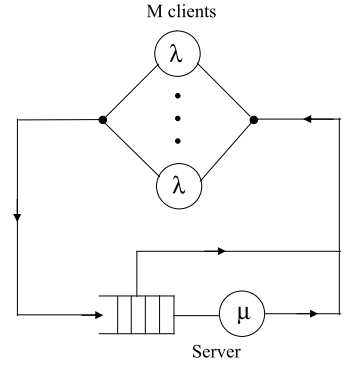
\includegraphics[scale=1]{figures/ex/cssystem.png}
\caption{Client-Server System}
\end{figure}

Client/Server con $M$ utenti. $\forall$ utente, in media dopo $\frac{1}{\lambda} s$ (EXP NEG) invia una richiesta al server. Il server esegue le richieste con FCFS. $\frac{1}{\mu} s$ è il tempo di servizio. Un utente genera una richiesta dopo che la precedente è stata servita. Ogni utente, indipendentemenete dagli altri, dopo un periodo di riflessione $(\frac{1}{\lambda})$, può quindi inviare le richieste al server. Gli utenti sono tuttavia impazienti e possono cancellare le richieste: a partire dall'invio delle richieste, dopo un tempo di durata media $\frac{1}{\gamma} s$, cancella la richiesta. Può cancellare solo se la richiesta NON sta venendo eseguita. Tempi di servizio, cancellazione e di riflessione sono rispettivamente i.i.d. e statisticamente indipendenti tra di loro; Quindi DTT, utilizzazione CPU, \dots

Modellazione di un sistema Web. Non è contemplata la possibilità che un utente si scocci e vada via. Condizioni di saturazione: Studio del sistema sotto-stress. $\max\{M\}$ per avere determinate prestazioni. Numero di utenti massimo che il server può sopportare, tollerare affinché si abbiano delle predeterminate prestazioni. $t\rightarrow \frac{1}{\lambda}$ per cliccare su un certo Hyperlink. 

Sistema reale Questo sistema reale descritto può essere modellato come una RETE DI CODE CHIUSA. Sistema a coda. Modello stocastico che rappresenta questo sistema reale descritto. Varie entità in gioco: \{\{utenti\}, server\}. Si parla di: \{tempi di riflessione, tempi di servizio, tempi di cancellazione\}. Server Web. Processo applicativo. Clienti + servitore + fila di attesa. Una rete di code è un insieme di code interconnesse tra di loro secondo una certa topologia. APERTA quando i clienti possono arrivare dall'esterno e partire verso l'esterno di questo sistema. CHUSA quando NON c'è la possibilità che arrivino dall'esterno o partano verso l'esterno. In tal caso il numero dei clienti è costante (Non si arriva e non si parte). Situazioni intermedie rendono il sistema non stabile. I blocchi di ritardo sono modellabili con delle code [$\mathord{\cdot}$/M/$\infty$]. Questa è una RETE DI CODE CHIUSA. $M=\cardinality{clienti}$. $M$ utenti nel sistema reale. Clienti + servitore. Un cliente si può trovare o nei blocchi di ritardo oppure nel sistema a coda. La presenza di un cliente nel blocco di ritardo rappresenta il fatto che nel sistema reale gli utenti possono avere un tempo di riflessione. Abbiamo $M$ unità di ritardo. Se un cliente è in un blocco di ritardo, il corrispondente utente nel sistema reale si trova in un periodo di riflessione. Il passaggio di un cliente dal blocco di ritardo verso il sistema a coda rappresenta il fatto che l'utente ha cliccato su un hyperlink: ha inviato una richiesta al server. Fila di attesa. Il passaggio di un cliente dalla fila di attesa verso il centro di servizio corrisponde al fatto che il server ha preso in considerazione la richiesta Web. Quando nel modello il cliente parte, andrà nuovamente nel blocco di ritardo. Il corrispondente utente nel sistema reale, avendo usufruito dell'erogazione del servizio, starà di nuovo pensando, scegliendo il successivo hyperlink da cliccare. C'è anche la possibilità che un cliente vada via dalla fila di attesa PRIMA ancora che venga servito. Ciò corrisponde alla situazione reale al fatto in cui un utente cancelli la propria richiesta in attesa, in coda. Possibilità che i clienti vadano via dalla fila di attesa. Anche quando un cliente va via dalla fila di attesa, giungerà nuovamente nei blocchi di ritardo. Modello stocastico che rappresenta bene il sistema reale.

Rete di code. Potrei risolverla con le tecniche adibite alla risoluzione di queste reti di code. Ma procederemo con i processi stocastici. Consideriamo il processo stocastico: $N(t)=\cardinality{clienti\ del\ sistema\ a\ tempo\ t}$ (Nel sistema a coda). Dinamica determinata dalle v.a.: \{tempi di riflessione, tempi di servizio, tempi di annullamento\}. Sono tutte v.a. exp-neg i.i.d. e statisticamente indipendenti tra di loro $\implies $ CMTC. DTT:

\begin{center}
\begin{tikzpicture}[->, >=stealth', auto, semithick, node distance=2.8cm]
\tikzstyle{every state}=[fill=white,draw=black,thick,text=black,scale=1]
\node[state]    (0)                     {$0$};
\node[state]    (1)[right of=0]   {$1$};
\node[state]    (2)[right of=1]   {$2$};
\node[state] (d) [right of=2] {\ldots};
\node[state]    (MM1)[right of=d]  {$M-1$};
\node[state]    (M)[right of=MM1]   {$M$};
\path
(0) edge[bend left]     node{$M\lambda$}         (1)
(1) edge[bend left]     node{$(M-1)\lambda$}         (2)
    edge[bend left,below]    node{$\mu$}            (0)
(2) edge[bend left]     node{$(M-2)\lambda$}           (d)
    edge[bend left,below]    node{$\mu+\gamma$}             (1)
(d) edge[bend left]         node{$(M-3)\lambda$}   (MM1)
	edge[bend left,below]   node{$\mu+2\gamma$}          (2)
(MM1)edge[bend left]    node{$(M-1)\lambda$}     (M)
     edge[bend left,below] node{$\mu+(M-2)\gamma$} (d)
(M) edge[bend left,below] node{$\mu+(M-1)\gamma$} (MM1);
\end{tikzpicture}
\end{center}

I clienti che NON si trovano nel sistema a coda saranno in una condizione di \underline{ARRIVO} nel sistema a coda. Il tempo che ci mette per uscire dal blocco di ritardo e giungere nel sistema a coda è $(\dots)\sim EXP-NEG(\lambda)$ i.i.d. indipendente dalle altre. Consideriamo uno stato non estremo. $0<i<M$. Supponiamo che al tempo $t$, $\underline{N(t)=i}=\cardinality{clienti\ in\ fila\ di\ attesa}+\cardinality{clienti\ nel\ centro\ di\ servizio}$. Avremo rispettivamente $i-1$ clienti in coda ed 1 nel centro di servizio. Se lo stato a tempo $t$ è i, avremo un certo numero $(M-i)$ in condizioni di arrivo. Se lo stato è i, la successiva transizione di stato potrà essere determinata da: un arrivo nel sistema a coda, quando finisce un servizio in corso, oppure a causa di un annullamento di una delle $(i-1)$ richieste pendenti. In questo caso, si avrà una transizione di stato (variazione di stato). $t \rightarrow$ successivo arrivo. Indichiamo al solito con $\xi_{R(t)}|_i\sim EXP ((M-i)\lambda) = \min\{(\dots)\}$, ovvero pari al minimo delle v.a. che rappresentano il tempo di arrivo residuo del k-esimo cliente nel blocco di ritardo (NO TEMPO DI INTERARRIVO!). Tempo che passa invece dall'istante $t$ al successivo completamento dell'erogazione del servizio è $\eta_{R(t)}|_i\sim EXP(\mu)$. Il tempo che passa dall'istante presente $t$ ed il successivo annullamento della richiesta è una v.a. definita in tal modo: $\theta_{R(t)}|_i\sim EXP[(i-1)\gamma]=\min\{(\dots)\}$, ovvero pari al minimo delle v.a. che rappresentano il tempo di annullamento residuo al tempo $t$. Ricordiamo: $\phi_i(t)\sim EXP(-q_{ii})$, ovvero il tempo di soggiorno nello stato $i$. Inoltre, $\Pr\{\phi_i(t)>\tau\}$, la sua CDF complementare, è pari alla probabilità che in $\tau$ NON ci sia nessun arrivo, NON ci sia la fine del servizio in corso e NON vi sia annullamento di una richiesta; il tutto condizionato con il fatto di trovarci nello stato $i$. Per indipendenza, essa è pari al prodotto delle rispettive probabilità, ovvero:

\[
	\Pr\{\phi_i(t)>\tau\} = [\Pr\{\xi_{R(t)} > \tau\ |\ i\}\Pr\{\eta_{R(t)} > \tau\ |\ i\}\Pr\{\theta_{R(t)} > \tau\ |\ i\}] =
\]
\[	
	= \e^{-(M-i)\lambda\tau}\e^{-\mu\tau}\e^{-(i-1)\gamma\tau} = e^{[\underline{-[(M-i)\lambda+\mu+(i-1)\gamma] = x]\tau}}
\]

Cosicché $(-q_{ii}=[x]) > 0$, ovvero abbiamo trovato la VELOCIT\`A TOTALE DI USCITA. Procediamo al solito modo:

\[
	\underline{\tau_{i,i+1}} = \frac{q_{i,i+1}}{-q_{ii}} = (\dots)
\]

dove $[-q_{ii}=[(M-i)\lambda+\mu+(i-1)\gamma]]$; il termine sottolineato è invece la probabilità che, lasciando lo stato $i$, migriamo verso lo stato $i+1$.

\[
	(\dots) = \Pr\{\xi_{R(t)} < \underline{\min\{\eta_{R(t)},\ \theta_{R(t)}\}}\} = (\dots)
\]

ove tale quantità rappresenta la probabilità che il successivo arrivo preceda il verificarsi dei due altri eventi. Tramite il teorema delle probabilità totali, otterremo alla fine:

\[
	(\dots) = \frac{(M-i)\lambda}{(M-i)\lambda+\mu+(i-1)\gamma} \implies
\]
\[
	\left\{
	\begin{aligned}
	&[q_{i,i+1} = (M-i)\lambda]\\
	&[q_{i,i-1} = \mu+(i-1)\gamma]
	\end{aligned}
	\right.
\]

Abbiamo quindi capito perché i tassi di transizione sono proprio questi. 

\[
	N(t)=0 \implies \underline{\phi_0(t)}\sim EXP(-q_{00}) =\underline{\xi_{R(t)}|_0} \sim EXP(M\lambda)
\]

$\implies \underline{-q_{00} = M\lambda}$. Se invece consideriamo lo stato $N(t)=M$ (tutti i clienti nel sistema a coda), avremo 0 clienti invece nel blocco di ritardo. La successiva transizione di stato sarà determinata o dall'annullamento di una richiesta o dalla fine dell'erogazione del servizio in corso:

\[
	\phi_M(t) = \min\{\eta_{R(t)}, \theta_{R(t)}\} \sim EXP((M-1)\gamma+\mu)
\]

$\implies -q_{MM} = (M-1)\gamma+\mu$. Quindi in realtà possiamo considerare valida la definizione di $-q_{ii}$ per $1<i\leq M$, in realtà.

CATENA \underline{\underline{ERGODICA}} $\iff$ OMOGENEA, IRRIDUCIBILE e $\cardinality{stati}<+\infty\iff$ numero di stati finito. Nel sistema a coda più di $M$ clienti NON ci possono essere $(\iff \cardinality{stati}<+\infty)$. 

CMTC tempo continuo, nascita e morte $\implies$

\[
	\left\{
	\begin{aligned}
	&[\pi_i=\pi_0 \lambda^i \frac{M!}{(M-i)!} \frac{1}{\prod_{k=0}^{i-1}{(\mu+k\gamma)}}]\\
	&\pi_0 = \frac{1}{1+\sum_{i=1}^M{\lambda^i \frac{M!}{(M-i)!} \frac{1}{\prod_{k=0}^{i-1}{(\mu+k\gamma)}}}}
	\end{aligned}
	\right.
\]

ove $\pi_0$ lo otteniamo con la condizione di NORMALIZZAZIONE. $i-1$ richieste pendenti ed un'altra in esecuzione nella CPU (del Server). $\rho$ è l'UTILIZZAZIONE, ovvero la frazione di tempo in media nella quale il servitore è impegnato a servire i clienti: $[\rho=1-\pi_0]$. Adesso dobbiamo valutare il throughput medio (throughput della CPU). Numero medio di richieste servite dalla CPU $\forall$ unità di tempo. Quando la CPU termina il servizio della richiesta, il cliente partirà dal centro di servizio. Applichiamo \underline{Little} ed otteniamo:

\[
	[\rho=\frac{\lambda_S}{\mu} \implies \lambda_S = \mu\rho = \mu(1-\pi_0)]
\]

Se consideriamo il prodotto $\pi_i[\mu+(i-1)\gamma]$, otteniamo la frequenza delle transizioni di questo tipo. Numero medio di volte che accade questa transizione $\forall$ unità di tempo. Consideriamo allora: $\underline{\pi_i\mu} + \underline{\pi_i(i-1)\gamma}$. Il primo termine sottolineato è la frequenza delle transizioni che portano da $i$ ad $i-1$ A CAUSA della fine di un servizio, mentre il secondo termine sottolineato rappresenta la frequenza delle transizioni $i\rightarrow i-1$ A CAUSA dell'annullamento di una richiesta. 

\[
	\left\{
	\begin{aligned}
	&[\lambda_S = \mu\pi_1 + \mu\pi_2 + \mu\pi_3 + \dots + \mu\pi_M = \mu(1-\pi_0) = \mu\rho]\\
	&[\lambda_R = \gamma\pi_2 + 2\gamma\pi_3 + 3\gamma\pi_4 + \dots + (M-1)\gamma\pi_M]
	\end{aligned}
	\right.
\]

Ove la seconda equazione rappresenta la velocità di partenza dei clienti dalla fila di attesa. Per trovare il numero medio di clienti in stato di riflessione, quindi, applichiamo nuovamente Little:

\[
	\bar{N}_R = \underline{(\lambda_S+\lambda_R)} \frac{1}{\lambda}
\]
\[
	\bar{N}_R = 0 \pi_M + 1\pi_{M-1} + 2\pi_{M-2} + \dots + M\pi_0
\]

Non è infatti difficile riconoscere ivi una media. Si può dimostrare che i due termini sono praticamente uguali e consistenti utilizzando le equazioni di BILANCIAMENTO LOCALE:

\[
	\pi_{i-1}(M-i+1)\lambda = \pi_i[(\mu+(i-1)\gamma)]
\]

Assumendo che le richieste NON possano essere cancellate, abbiamo che:

\[
	\underline{\E[R]} + \frac{1}{\lambda}
\]

Il primo termine sottolineato è il tempo medio di risposta, ove con $R$ intendiamo il tempo di risposta del sistema a coda, mentre il secondo addendo è al solito il tempo medio di riflessione. Un utente invierà una richiesta ogni $(\E[R]+\frac{1}{\lambda})$. Abbiamo $M$ richieste. $M$ utenti invieranno $M$ richieste alla seguente velocità:

\[
	(\frac{M}{\E[R]+\frac{1}{\lambda}}) = \underline{\lambda_S} = \mu\rho
\]

Dato che un utente NON può inviare una richiesta PRIMA che la precedente sia soddisfatta. Ove adesso il termine sottolineato rappresenta la velocità di arrivo delle richieste. Cosicché abbiamo:

\[
	\frac{M}{\mu\rho} = \E[R]+\frac{1}{\lambda} \implies \E[R] = \frac{M}{\mu\rho} -\frac{1}{\lambda} \implies \E[R]=\mathord{\cdot}{(M)}
\]

Se abbiamo 1 solo cliente $\iff M\rightarrow 1 \implies \E[R]=\frac{1}{\mu}$ NO fila di attesa. $M\uparrow (\mathord{\cdot}\to\infty) \implies \rho\to1 \implies \E[R]=(\frac{M}{\mu}-\frac{1}{\lambda})$, la quale quantità corrisponderebbe all'ASINTOTO OBLIQUO del grafico di $\E[R]$ in funzione di $M$.

L'asintoto viene in letteratura chiamato \textit{HEAVY LOAD asymptote}, mentre la retta ovviamente corrisponderebbe al \textit{LIGHT LOAD asymptote}. Il valore di $M$, $M^\star$ per il quale i due asintoti si incontrano, viene chiamato in letteratura \textit{SATURATION NUMBER}, ovvero il valore di $M=M^\star$ per il quale il sistema si considera in SATURAZIONE. Carico che può essere tollerato da un servizio, da un server:

\[
	\frac{1}{\mu} = \frac{M}{\mu} -\frac{1}{\lambda} \implies \frac{M}{\lambda} = \frac{1}{\mu}+\frac{1}{\lambda} \implies M^\star = (1+\frac{\mu}{\lambda})
\]

Tale valore rappresenta quindi il valore di $M$ per il quale il sistema è in saturazione. Se $\frac{1}{\lambda}=15 s$, e nel caso in cui $\frac{1}{\mu}=1 s$, abbiamo $\implies M^\star = 16 = 1+(15=\frac{\mu}{\lambda})$.

Ricordiamo che:

\[
	\underline{R(t) = \Pr\{X > t\}}
\]

è l'AFFIDABILIT\`A.

\subsection{RECAP}

M/M/1. Stato: $N(t) := \cardinality{clienti\ nel\ sistema\ a\ coda}$ (nell'intero sistema a coda). $N_q(t) := \cardinality{clienti\ in\ fila\ di\ attesa}$. CATENA DI MARKOV (OMOGENEA). Noto lo stato presente è possibile determinare l'evoluzione futura del processo in termini probabilistici, senza conoscere la storia passata (lo stato presente riassume tutta l'evoluzione passata). CATENE = stato discreto. Dell'evoluzione futura fa parte anche il tempo di soggiorno residuo $\phi_i(t) \sim EXP(-q_{ii})$. Se noto lo stato del processo nell'istante presente non riesco a determinare la distribuzione del tempo di soggiorno residuo, nel tempo in cui mi trovo, possiamo dire che NON riusciamo a determinare l'evoluzione futura. Evoluzione futura in termini probabilistici.

M/M/1. $\cardinality{clienti\ in\ fila\ di\ attesa}=\underline{N_q(t) = 0}$. Supponiamo vi siano 0 clienti (informazione che ho sullo stato presente del processo). Proviamo a determinare la distribuzione del tempo di soggiorno residuo in questo istante, MA non so se ci sono clienti nel centro di servizio. 

Supponiamo che vi sia un cliente nel centro di servizio (servitore occupato). Se termina quel servizio, si avrà una transizione di stato? NO. $\underline{\phi_0}(t)$ (0 clienti in fila di attesa). Se c'è 1 cliente, $\phi_0(t)\sim EXP(\lambda)$. Tempo di interarrivo residuo. Ma se non c'è nessuno, quella v.a. non sarà mica pari al tempo di interarrivo residuo. La transizione di stato si ha se arriva un cliente e ne arriva un altro. (Quindi se mettiamo insieme l'informazione invece riusciamo). Ma se includiamo quell'informazione torniamo alla precedente definizione di stato.

\section{RETI DI CODE}

Una rete dati di tipo switched può essere modellata mediante una rete di code. Queste code interagiscono tra di loro. Uno stream di pacchetti in partenza da una coda potrà andare a visitare un'altra coda dopo un merging con pacchetti provenienti da un'altra coda. [MERGING = POOLING]. Quindi una volta acceduti alla rete (superata la coda di accesso), si crea (si viene a creare) una correlazione tra i tempi di interarrivo dei pacchetti e quelli di trasmissione. Quindi viene meno l'ipotesi iniziale di indipendenza tra tempi di servizio e tempi di interarrivo. Adesso i tempi di servizio corrispondono ai tempi di trasmissione. Immaginiamo che i pacchetti arrivino alla rete con un processo di $\lambda$-POISSON. Nodo di accesso. Supponiamo che le lunghezze dei pacchetti siano v.a. equidistribuite statisticamente (i.d.), mutuamente indipendenti (con un certo valor medio), ed indipendenti dai tempi di interarrivo dei pacchetti al nodo di accesso. Tempi di trasmissione $\sim EXP(\mathord{\cdot})$. Data una certa capacità, le lunghezza dei pacchetti sono collegate ai tempi di trasmissione. Supponiamo che tempi di elaborazione e propagazione siano trascurabili. FCFS disciplina di coda. Serve però un'ipotesi aggiuntiva riguardo la dimensione dei buffer $(d=+\infty)$, ovvero illimitata.

Sistema reale: insieme dei due router con linee random (coda in serie). Il primo sistema è un M/M/1, per le ipotesi fatte. Si osservi il ramo che collega il primo centro di servizio con l'ingresso nel secondo buffer, e si effettuino delle analisi sulla eventuale dipendenza tra tempi di servizio e tempi di interarrivo. \`E evidente che le due grandezze sono in \textit{CORRELAZIONE}. Non posso quindi parlare di coda M/M/1 per il secondo sottosistema. A parte che non sappiamo che processo degli arrivi sia. Lo sapremo mediante teorema di \underline{BURKE}.

\begin{center}
\begin{figure}[H]
\centering
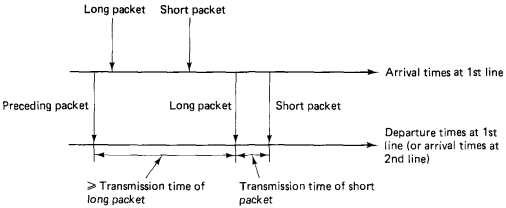
\includegraphics[scale=1]{figures/klnrk.png}
\caption{Timing Diagram of packet arrivals and departures completions in a system of two transmission lines in tandem} 
\end{figure}
\end{center}

Supponiamo che ad un certo istante termini la trasmissione di un pacchetto precedente. Poi, arrivi un pacchetto grande alla prima coda, il quale, trovandola vuota e notando disponibile il centro di servizio, ivi vi entra subito e viene iniziato il servizio (trasmissione). Finita la trasmissione di questo pacchetto, possiamo osservare che il tempo di interarrivo alla seconda coda (distanza temporale tra l'istante di arrivo del precedente pacchetto e l'istante di arrivo di questo), è risultato maggiore del tempo di trasmissione del pacchetto grande. Questo sarebbe già sufficiente per compromettere l'indipendenza. Si noti comunque che, se durante la trasmissione arriva un piccolo pacchetto alla prima coda, trovando il centro di servizio occupato, è costretto ad attendere in fila di attesa. Quando finirà la trasmissione del pacchetto grande, il piccolo potrà essere trasmesso. Ma a questo punto osserveremo un tempo di interarrivo (tra il grande ed il piccolo pacchetto) alla seconda coda praticamente uguale al tempo di trasmissione del piccolo pacchetto. Notiamo che vale: $\underline{t_{IA}\geq t_T}$, ovvero il tempo di interarrivo al secondo router è maggiore uguale del tempo di trasmissione nel primo router (in particolare sarà più grande se e solo se il secondo pacchetto trova la prima coda vuota (incluso il centro di servizio) al suo arrivo). Dal momento che nelle reti dati tipicamente avremo una lunghezza costante dei pacchetti, saranno quindi correlati anche i tempi di interarrivo al secondo sottosistema con i suoi tempi di servizio, dal momento che le lunghezze dei pacchetti influenzano i tempi di trasmissione, e quindi di servizio, anche se capacità dei link è differente tra i due. $\implies$ NO INDIPENDENZA. Leonard Kleinrock, il pioniere nella Ricerca delle Reti delle Code, ha risolto brillantemente questo problema. Andare a combinare (MERGING) su una certa coda flussi di pacchetti provenienti da altre code ha l'effetto di ripristinare l'indipendenza tra tempi di interarrivo a tempi di trasmissione. Se nel nostro esempio osserviamo al secondo router pacchetti di un altro router (nodo), non c'è più correlazione! Ripristino dell'ipotesi di INDIPENDENZA. La possibilità che accada questo evento dipende dal livello di comunicazione e di traffico! Più la rete è magliata (più merging di differenti flussi), e più è intenso il traffico, più è probabile che accadano eventi di questo tipo. La rete deve essere \textit{DENSAMENTE CONNESSA} ed il traffico deve essere intenso. Cosicché per una rete densamente connessa e per intensità di traffico medio-alta, possiamo ritenere valida la cosiddetta \textit{\textbf{APPROSSIMAZIONE DI INDIPENDENZA DI KLEINROCK}}. Intensità di traffico medio-alta inoltre! Possiamo mantenere sempre valida l'indipendenza tra tempi di interarrivo e tempi di trasmissione (servizio).

\subsection{RETE DI CODE APERTA}

Rete di code: insieme di code interconnesse tra di loro. Supponiamo di avere il seguente scenario:



Stiamo rappresentando con una rete di code un sistema di Elaborazione.

Clienti/Servitori/Fila di Attesa. Questa è la topologia della rete di code. Stiamo modellando un sistema di elaborazione. I clienti corrispondono alle richieste di esecuzione dei job (la presenza di un clientre in $\mu_1$ significa che si sta eseguendo quel job). I job stanno arrivando dall'esterno. Nodi alias stazioni di servizio. Il nodo 0 corrisponde al mondo esterno, dal quale possono arrivare i clienti. SINGLE CLASS \underline{OPEN}. Una rete si dice \underline{aperta} quando i clienti possono arrivare dall'esterno e fluire (partire) verso l'esterno. Per una CHIUSA (\underline{CLOSED}) è il contrario di quella aperta. Per una CHIUSA il numero di clienti è costantè (\textit{ISARITHMIC CONGESTION CONTROL}). $\exists M$ percorsi nella rete. Una rete di code, quando in essa i clienti arrivano esattamente se partono gli altri: 1 entra $\leftrightarrow$ 1 esce, può essere considerata chiusa. A volte possiamo volutamente limitare ad $M$ il numero di pacchetti che transitano. 

\underline{SINGLE CLASS OPEN}. Tornando al nostro caso, i clienti arrivando dall'esterno nel nostro sistema a coda, possono visitare solo il nodo 1 $\iff \underline{\underline{p_{01}=1}}$. Ma potrebbero $\exists(p_{0i}\neq 1)$. Leggi delle probabilità:

\[
	[p_{11}+p_{10}+p_{12}+p_{13}+p_{14} = 1]
\]

Similmente per gli altri nodi. Una volta visitato il nodo 2, il cliente potrà visitare soltanto il nodo 1. Questo vale anche per gli altri nodi 3-4! ($\iff [p_{21}=p_{31}=p_{41}=1]$. SINGLE CLASS = \{singola classe di clienti\}. Ma potrebbero esserci più classi di clienti. Per una rete di code con vari nodi definiamo:

\[
	[\underline{p_{ij} := ROUTING\ PROBABILITY}]
\]

o \underline{PROBABILIT\`A DI ROUTING}. (collegate ai protocolli di instradamento). Si potrebbero definire delle probabilità per differenti classi. Per altri stream potrei scegliere delle differenti destinazioni. Si modellino i vari stream nella rete ($\exists K$ classi ad esempio) come delle "classi di clienti". Sia: $N=\cardinality{nodi}$. Indichiamo con $K$ il vettore riga: $\underline{K} := (K_1,K_2,\ \dots,\ K_N)$, ove tale vettore rappresenta il numero di clienti NEI VARI NODI. Difatti, $K_i:=\cardinality{clienti\ al\ nodo\ "i"}$. E quindi: $K=\sum_{i=1}^N{K_i} := \cardinality{clienti\ nella\ rete}$. Definiamo: $[m_i\geq 1]:=\cardinality{servitori\ paralleli\ al\ nodo\ "i"}$. Indichiamo con $\mu_i$ la velocità del singolo servitore al nodo "i" (In generale possiamo avere velocità differenti per il nodo "i"). Noi considereremo servitori alla stessa velocità. Introduciamo il concetto di [Soluzione in forma PRODOTTO].

$p_{ij}$ = probabilità di routing $\implies p_{0,j}$ = probabilità che un cliente in arrivo dall'esterno vada a visitare il nodo $j$. Similmente, $p_{i,0}$ = probabilità che un cliente in partenza dal nodo $i$, lasci la rete. Cosicché: $pi_{i,0} = 1-\sum_{j=1}^N{p_{ij}}$. $\lambda_{0i}$ = velocità di arrivo dei clienti dall'esterno al nodo "i". Indichiamo con $\lambda$ la velocità totale di arrivo dei clienti dall'esterno $\iff \lambda=\sum_{i=1}^N{\lambda_{0i}}$. La velocità totale sarà tale che: $\lambda_{0i}=\lambda p_{0i}$. Indicando con $\lambda_i$ la velocità TOTALE di arrivo dei clienti al nodo $i$ e con $\lambda_j$ la velocità di partenza delle altre code, otteniamo:

\[
	[\lambda_i=\lambda_{0i}+\sum_{j=1}^N{\lambda_jp_{ji}}]
\]

con $i=1,2,\ \dots,\ N$. Dividendo membro a membro per $\lambda$ otteniamo:

\[	
	\frac{\lambda_i}{\lambda} = \frac{\lambda_{0i}}{\lambda} + \sum_{j=1}^N{\frac{\lambda_j}{\lambda}p_{ji}}
\]

con $i=1,2,\ \dots,\ N$. Queste sono le cosiddette \underline{EQUAZIONI DEL TRAFFICO}. Definiamo allora:

\begin{defn}{\textbf{Visit Ratio}}

Definiamo il VISIT Ratio come:

\[
	[e_i := \frac{\lambda_i}{\lambda}]
\]
\end{defn}

Esso rappresenta il numero medio di visite al nodo "i" $\forall$ arrivo dall'esterno. Quante volte un cliente IN ARRIVO DALL'ESTERNO visita il nodo "i" prima di lasciare la rete. Ad esempio:

\[	
	\lambda_i=20\ clienti/s,\ \lambda=2\ clienti/s,\ \frac{\lambda_i}{\lambda}=(10/2 = 5)\ clienti/s
\]

Diamo ora un'altra definizione:

\begin{defn}{\textbf{Service Demand}}

Definiamo $D_i$ service demand la quantità totale di servizio che in media un cliente richiede in un certo nodo:

\[
	\left\{
	\begin{aligned}
	&[e_i = p_{0i} + \sum_{j=1}^N{e_jp_{ji}}]\\
	&[D_i := e_i(\frac{1}{\mu_i})]
	\end{aligned}
	\right.
\]

\end{defn}

Si noti che $D_i$ è una quantità temporale!


Consideriamo la seguente rete di code: Due code a singolo router in serie e supponiamo che il processo degli arrivi al nodo "1" sia di $\lambda$-POISSON, che i tempi di servizio dei clienti alla prima ed alla seconda coda siano v.a. $(\dots)\sim EXP(\mu_1)$ per la prima e $(\dots)\sim EXP(\mu_2)$ per la seconda, mutuamente indipendenti ed \underline{indipendenti} dal processo degli arrivi alle code (tempi di interarrivo dei clienti alle code). QUESTE NON SONO RETI DATI! Ma generiche reti di code. Supponiamo $(d=+\infty)$ e disciplina di coda FCFS. Con le ipotesi viste la prima coda è M/M/1. Riguardo alla seconda coda, il processo degli arrivi dei clienti alla seconda coda corrisponde al tempo di partenza (al processo delle partenze dei clienti del nodo 1). Quindi è una $\mathord{\cdot}$/M/1 (Il processo degli arrivi NON può essere considerato, descritto indipendentemente dal resto della rete). Processo delle partenze. Questo fatto ci fa comprendere l'importanza di caratterizzare i processi delle partenze dei clienti delle code. Teorema di BURKE che fa la caso nostro:

\begin{thrm}{\textbf{Teorema di BURKE}}

Si consideri un sistema a coda M/M/1 $\lor$ M/M/m $\lor$ M/M/$(m=\infty)$. Sia $\lambda$ la velocità di arrivo dei clienti (processi degli arrivi dei clienti). Supponiamo di stare in condizioni di regime:

\begin{itemize}

\item{a)} Il processo delle partenze è \underline{di POISSON}, a velocità $\lambda$;
\item{b)} $\forall$ istante $t$, $\cardinality{clienti\ nel\ sistema}$ NON dipende dalla sequenza delle partenze fino a $t$. Esso dipende SICURAMENTE dagli arrivi che ci sono stati fino a $t$, SICURAMENTE dai tempi di servizio dei clienti che SONO stati effettivamente serviti;
\end{itemize}
\end{thrm}

Per dimostrarlo si dovrebbero utilizzare le CATENE DI MARKOV \textit{REVERSIBILI} (Ragionare andando nel verso opposto come tempo $\iff$ guardando l'evoluzione a ritroso).
Determinare la cosiddetta \textit{OCCUPANCY DISTRIBUTION}, ove intendiamo la probabilità che vi siano $K_1$ clienti nella "coda 1" e $K_2$ clienti nella "coda 2" a regime (probabilità congiunta):

\[
	\Pr\{K_1\ clienti\ nella\ "coda\ 1",\ K_2\ clienti\ nella\ "coda\ 2"\} =
\]
\[
	= \Pr\{K_1,K_2\} := \underline{\pi(K_1,K_2)}
\]

Notazione con pedici anche possibile. Distribuzione congiunta dei clienti nelle VARIE CODE. Una rete di code si dice STABILE se $\forall$ sistema a coda di cui si compone è STABILE. CONDIZIONE DI STABILIT\`A:

\[	
	[(\rho<1) \iff (\frac{\lambda}{\mu} < 1) \iff \lambda<\mu] \implies
\]
\[
	\implies
	\left\{
	\begin{aligned}
	&\rho_1=\frac{\lambda}{\mu_1} < 1 \iff \lambda<\mu_1\\
	&\rho_2=\frac{\lambda}{\mu_2} < 1 \iff \lambda<\mu_2
	\end{aligned}
	\right.
\]

Imposta la stabilità delle code e delle reti di code, utilizzo il teorema di BURKE. Sfruttiamo la parte a) del teorema. Processi degli arrivi in 2 di POISSON. Se guardiamo "2", isolatamente sarebbe un M/M/1 adesso (grazie a BURKE). Sfruttiamo adesso la parte b) di BURKE. Consideriamo le v.a. casuali che rappresentano il numero di clienti in "1" ed in "2":

\[
	\Pr\left\{
	\begin{aligned}
	&N_1(t) = K_1\\
	&N_2(t) = K_2
	\end{aligned}
	\right.
\]

Abbiamo $\{N_1(t),N_2(t)\},\ \forall t$. Risulta:

\[
	N_1(t) \neq \mathord{\cdot} N_2(t)
\]

grazie a Burke $\implies N_1(t),N_2(t)$ sono v.a. indipendenti $\implies$

\[
	\pi_{K_1,K_2} := \pi(K_1,K_2) = \pi(K_1)\pi(K_2)
\]

pari ovvero al prodotto delle due distribuzione marginali dei sistemi a coda visti in isolamento. Soluzione in FORMA PRODOTTO della OCCUPANCY DISTRIBUTION. In realtà i singoli sistema a coda NON stanno in isolamento! \`E una rete di code infatti. Riprendendo l'esempio delle M/M/1, abbiamo:

\[
	\{\lambda,\mu\} \implies \underline{\pi(K_1,K_2)} = [(1-\rho_1)\rho_1^{K_1}][(1-\rho_2)\rho_2^{K_2}]
\]

dove abbiamo: $\{(\rho_1=\frac{\lambda}{\mu_1}),\ (\rho_2=\frac{\lambda}{\mu_2})\}$. Ove abbiamo semplicemente utilizzato le espressioni trovate per la M/M/1. Allo stesso risultato si poteva arrivare senza sfruttare Burke ed analizzando con approccio Markoviano le seguenti reti di code, utilizzando una definizione di stato bidimensionale (multi-indice) (al tempo $t$). Sfruttiamo l'EQ. DI BILANCIAMENTO TOTALE dei flussi per una CATENA ERGODICA. Dovremo però aggiungere ovviamente la condizione di normalizzazione. Si arriva a scrivere:

\[
	\pi_{K_1,K_2} = (1-\frac{\lambda}{\mu_1})(1-\frac{\lambda}{\mu_2})(\frac{\lambda}{\mu_1})^{K_1}(\frac{\lambda}{\mu_2})^{K_2} =
\]
\[	
	= [\underline{((1-\frac{\lambda}{\mu_1})(\frac{\lambda}{\mu_1})^{K_1} = \pi_1(K_1))}][\underline{((1-\frac{\lambda}{\mu_2})(\frac{\lambda}{\mu_2})^{K_2} = \pi_2(K_2))}] = \underline{\pi(K_1)\pi(K_2)}
\]

Proviamo a sostituirle nelle equazioni di bilanciamento.

Giustificazione matematica. $\underline{(K_1,K_2)}$. Quindi ai fini della \underline{Occupancy Distribution}, la distribuzione congiunta è pari al prodotto delle distribuzioni marginali.

\subsection{Feed-Forward (Reti di code ACICLICHE)}

Tutte le reti di code che comprendono code del tipo: \{$\mathord{\cdot}$/M/1, $\mathord{\cdot}$/M/m, $\mathord{\cdot}$/M/$\infty$\} le quali ricevono arrivi sia da altre code della rete, sia dall'esterno, secondo processi di POISSON, e che non permettono a nessun cliente di ritornare ad una coda già visitata (SENZA CICLI), sono risolubili in forma prodotto. ACICLICHE $\iff \nexists$ CICLI. Per come sono fatte queste reti di code i processi degli arrivi sono di POISSON alle varie CODE.

\subsubsection{SEARCH ENGINE - MOTORI DI RICERCA}

Si consideri una porzione di rete in cui sono presenti tre motori di ricerca organizzati gerarchicamente in due livelli (vedi figura): a livello più alto e’ presente il motore MC, mentre a livello gerarchico più basso sono presenti i motori MA e MB. Gli utenti sono connessi al livello gerarchico più basso. Una richiesta di ricerca viene presentata da un generico utente al proprio motore. Questo, se dopo averla elaborata, non e’ in grado di soddisfarla, la reindirizza verso il motore MC che e’ sicuramente in grado di risolverla. Si assuma che:

\begin{itemize}

\item{i)} le richieste di ricerca da parte degli utenti del gruppo A siano presentate in accordo ad un processo di Poisson con parametro $\lambda_A\ req/min$;
\item{ii)} le richieste di ricerca da parte degli utenti del gruppo B siano presentate in accordo ad un processo di Poisson con parametro $\lambda_B\ req/min$;
\item{iii)} in ogni motore un unico processore elabori le richieste in modalità FCFS e con tempi che sono v.c. indipendenti distribuite secondo una ddp esponenziale negativa a valor medio pari, rispettivamente per i tre motori $M_A$, $M_B$, e $M_C$, a $T_A$ sec, $T_B$ sec e $T_C$ sec;
\item{iv)} una richiesta sia soddisfatta con probabilità $\alpha$ da un motore di livello basso;
\item{v)} sia trascurabile il tempo necessario ad inoltrare una richiesta al motore $M_C$.  

\end{itemize}

Calcolare:

\begin{itemize}

\item{a)} il fattore di utilizzazione del processore nel motore $M_C$;
\item{b)} il tempo medio di risoluzione di una richiesta;
\item{c)} il tempo medio di risoluzione di una richiesta da parte degli utenti del gruppo A. 
  
\end{itemize}

\begin{center}
\begin{figure}[H]
\centering
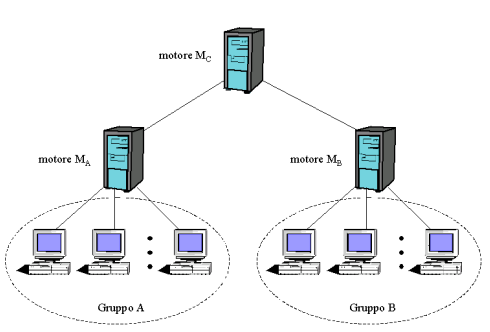
\includegraphics[scale=1]{figures/ex/se.png}
\caption{Hierarchical Search Engines}
\end{figure}
\end{center}

Risoluzione:

Tre motori di ricerca organizzati gerarchicamente in tre livelli. Gli utenti sono connessi al livello gerarchico più basso. $\{\lambda_A,\lambda_B\}\ req/min$, processi di POISSON. Richieste in modalità FCFS. Per quanto concerne i tempi di servizio, siamo dinanzi delle ddp esponenziali con i seguenti tempi di servizio medi, rispettivamente: $\{T_A, T_B, T_C\}s$. $M_C=?$ (fattore di utilizzazione). C'è da aggiungere un'ipotesi sulle dimensioni delle file di attesa: File di attesa illimitate $\iff (d=+\infty)$. Se qualcuna fosse un collo di bottiglia ci sarebbe scritta la dimensione $(\iff d<+\infty)$. Reti di code ACICLICHE. Processo degli arrivi dall'esterno di POISSON. Processo degli arrivi alle varie code di POISSON. Applicabile/applicato il teorema di BURKE. Abbiamo: $\{\mu_A=\frac{1}{T_A},\ \mu_B=\frac{1}{T_B},\ \mu_C=\frac{1}{T_C}\}$. Parametri della ddp esponenziale negativa. Popolazione illimitata $\iff (e=+\infty)$. Processo degli arrivi di POISSON. Rete ACICLICA $\iff$ feedforward network. Mi trovo dinanzi una rete di code. I processi degli arrivi sono di POISSON. Le reti A e B sono delle M/M/1. Viste in isolamento sono delle M/M/1. $\{K_A,\ K_B,\ K_C\}$ ci servono per definire la Occupancy Distribution (Burke + Splitting/Pooling). Code M/M/1 viste in isolamento $\iff$ grazie alla Soluzione in forma prodotto. Dobbiamo applicare le EQUAZIONI DEL TRAFFICO. La velocità di arrivo al sistema $M_C$ sarà:

\[
	\lambda_A(1-\alpha) + \lambda_B(1-\alpha) = (1-\alpha)(\lambda_A+\lambda_B) := \lambda_C
\]

I clienti NON si perdono! Se $\lambda_A$ arrivano nel primo sistema, $\lambda_A$ ne partiranno! Lo stesso dicasi per $M_C$. Per la STABILIT\`Adella rete di code dobbiamo imporre che $\forall$ sistema vi sia STABILIT\`A. Stabilità di ogni singolo sistema a coda:

\[
	\left\{
	\begin{aligned}
	&\rho_A = \frac{\lambda_A}{\mu_A}<1 \iff \lambda_A<\mu_A\\
	&\rho_B = \frac{\lambda_B}{\mu_B}<1 \iff \lambda_B<\mu_B\\
	&\rho_C = \frac{\lambda_C}{\mu_C}<1 \iff \lambda_C<\mu_C
	\end{aligned}
	\right.
\]

Analogamente... tre motodi di ricerca. Livello didattico. Nel calcolare $\lambda_C$ abbiamo anche risolto la prima domanda: $\rho_C=\frac{\lambda_C}{\mu_C}$, ovvero il FATTORE DI UTILIZZAZIONE del servitore nel nodo $M_C$. 

Tempo medio di risoluzione di una richiesta. L'arrivo nella rete di code di una richiesta corrisponde all'invio di una richiesta da parte di un utente. Tempo medio di risoluzione di una richiesta = tempo medio di permanenza nell'intero sistema. Clienti dall'esterno + Clienti in partenza $\leftarrow$ risoluzione di una richiesta. Si applichi Little:

\[
	[\bar{N}_{TOT} = \lambda_{TOT}\bar{R}] \implies \bar{R} = \frac{\bar{N}_{TOT}}{\lambda_{TOT}}
\]

$\bar{R}$ è quello che mi interessa. Sappiamo che: $\underline{\lambda_{TOT} = \lambda_A+\lambda_B}$, ovvero la velocità totale di arrivo dei clienti dall'esterno. Per un M/M/1 $\mathord{\cdot}(\lambda,\mu)$ il numero medio di clienti è: $(\bar{N}=\frac{\lambda}{\mu-\lambda})$. Lo dobbiamo però applicare ai vari sottosistemi. Somma dei numeri medi di clienti (a regime ovviamente):

\[
	[N_{TOT}=\bar{N}_A+\bar{N}_B+\bar{N}_C]\\
\]

sapendo che:

\[
	\left\{
	\begin{aligned}
	&\bar{N}_A = \frac{\lambda_A}{\mu_A-\lambda_A}\\
	&\bar{N}_B = \frac{\lambda_B}{\mu_B-\lambda_B}\\
	&\bar{N}_C = \frac{\lambda_C}{\mu_C-\lambda_C}
	\end{aligned}
	\right.
\]

Quindi abbiamo:

\[
	\bar{R} = \frac{N_{TOT}}{(\lambda_A+\lambda_B=\lambda_{TOT})}
\]

Per sapere invece il tempo medio di risoluzione di una richiesta da parte degli utenti del gruppo A $\iff R_A=?$, sapendo che per un M/M/1 vale:

\[
	\left\{
	\begin{aligned}
	&\bar{N}=\frac{\lambda}{\mu-\lambda}\\
	&\bar{T}=\frac{1}{\mu-\lambda}
	\end{aligned}
	\right.
\]

Allora si riconosce subito la media di una v.a.:

\[
	\bar{R}_A = \alpha[\frac{1}{\mu_A\lambda_A}] + (1-\alpha)[\frac{1}{\mu_A\lambda_A} + \frac{1}{\mu_C-\lambda_C}] =
\]
\[
	=  \frac{\alpha}{\mu_A-\lambda_A}+\frac{1}{\mu_A-\lambda_A}-\frac{\alpha}{\mu_A-\lambda_A}+\frac{1}{\mu_C-\lambda_C}-\frac{\alpha}{\mu_C-\lambda_C} =
\]
\[
	= [\frac{1}{\mu_A-\lambda_A}+\frac{(1-\alpha)}{\mu_C-\lambda_C}]
\]

Legittimo applicare Little al sottosistema $M_C$. Potremmo in realtà tentare un altro approccio. Potrei applicare Little a tutto il sistema ma considerando il numero di clienti del gruppo A. Sappiamo che:

\[
	\bar{N}_C = \frac{\lambda_C}{\mu_C-\lambda_C}
\]

Ma non stiamo diversificando i gruppi di clienti. La frazione di clienti A in $M_C$ è: $\frac{\lambda_A(1-\alpha)}{\lambda_C}$. Se facciamo questo rapporto, questa quantità corrisponderà proprio alla frazione dei clienti del gruppo A in $M_C$. Possiamo quindi scrivere la formula per sapere il numero medio di clienti del gruppo A in tutta la rete di code:

\[
	\bar{N}_{TOT,A} = ? = \frac{\lambda_A}{\mu_A-\lambda_A}+(\frac{\lambda_A(1-\alpha)}{\lambda_C})(\frac{\lambda_C}{\mu_C-\lambda_C}) = \frac{\lambda_A}{\mu_A-\lambda_A} + \frac{\lambda_A(1-\alpha)}{\mu_C-\lambda_C} =
\]
\[
	= \lambda_A[\frac{1}{\mu_A-\lambda_A}+\frac{(1-\alpha)}{\mu_C-\lambda_C}]
\]

Dobbiamo ora applicare Little:

\[
	\frac{\bar{N}_{TOT,A}}{\lambda_A} = \bar{R}_A = [\frac{1}{\mu_A-\lambda_A}+\frac{(1-\alpha)}{\mu_C-\lambda_C}]
\]

avendo considerato come velocità di arrivo solo $\lambda_A$, ovviamente.

\subsection{Reti di code CICLICHE}

Fino ad ora abbiamo visto le reti ACICLICHE $\iff$ Non permettiamo ad un cliente di visitare una coda già visitata. L'assenza di cicli è fondamentale per preservare la caratteristica di POISSON. Ciononostante esistono delle reti di code con CICLI per le quali continua comunque a valere la Soluzione in forma prodotto per la Occupancy Distribution. Reti di code con CICLO. Parliamo di rete aperta naturalmente. Due code $\mathord{\cdot}$/M/1 collegate in serie e con CICLO. Stiamo facendo l'ipotesi che i tempi di servizio siano v.a. distribuite esponenzialmente, mutuamente indipendenti e statisticamente indipendenti dai tempi di interarrivo dei clienti, distribuiti secondo $\lambda$-POISSON. 

\subsubsection{JACKSON NETWORK}

\underline{JACKSON NETWORK}. $\{p := p_1,\ p_2 := 1-p\}$. Ci favorisce la possibilità di calcolare la Occupancy Distribution sempre utilizzando la Soluzione in forma prodotto. Occupancy Distribution utilizzando una soluzione di stato bidimensionale $\{N_1(t),\ N_2(t)\}$. Processo stocastico. Due code $\mathord{\cdot}$/M/1. Fila di attesa illimitata $\iff (d=+\infty)$. Altrimenti non potrei parlare di M/M/1. Le ACICLICHE sono un sottoinsieme delle reti di JACKSON. Una rete di JACKSON senza cicli è una rete ACICLICA. Vale:

\[
	\lambda_1=\lambda+\lambda_2\alpha \stackrel{[\lambda_2=\lambda_1]}{=} \lambda+\lambda_1\alpha \implies
\]
\[
	\implies [\lambda_1 = \frac{\lambda}{1-\alpha} = \lambda_2]
\]

Dobbiamo imporre anche qui la STABILIT\`A dei singoli sottosistemi:

\[
	\left\{
	\begin{aligned}
	&\rho_1 := \frac{\lambda_1}{\mu_1} < 1 \iff \lambda_1<\mu_1\\
	&\rho_2 := \frac{\lambda_2}{\mu_2} < 1 \iff \lambda_2<\mu_2
	\end{aligned}
	\right.
\]

Adottiamo l'approccio precedente. Dobbiamo srivere le EQ. di bilanciamento totale dei flussi. Qui ovviamente NON possiamo applicare BURKE. I processi degli arrivi non sono di POISSON. Abbiamo scritto le equazioni di bilanciamento totale dei vari flussi. Dovrei risolvere il sistema aggiungendo la condizione di NORMALIZZAZIONE. Ricordiamo che: $\cardinality{stati}=+\infty$. Proviamo ad utilizzare questa distribuzione:

\[
	[\pi_{K_1,K_2} = \underline{(1-\frac{\lambda_1}{\mu_1})(\frac{\lambda_1}{\mu_1})^{K_1}} \underline{(1-\frac{\lambda_1}{\mu_2})(\frac{\lambda_2}{\mu_2})^{K_2}}]
\]

Ove i termini sottolineati sommano ad 1. Si può verificare che, dato che sostituite nella eq. di bilanciamento totale dei flussi essa è risolta $\iff$ è proprio quella la distribuzione. Prodotto delle distribuzioni marginali dei singoli sottosistemi, considerando che la loro distribuzione degli arrivi sia di POISSON, anche se in realtà non lo è! Sono sicuro che gli arrivi NON sono distribuiti secondo POISSON, ma i singoli sottosistemi, ai fini del calcolo della Occupancy Distribution, è proprio come se fossero degli M/M/1 in ISOLAMENTO! $\lambda$-POISSON autorizzati. Esempio di reti di code per le quali vale anche la Soluzione in forma prodotto $\rightarrow$ \underline{JACKSON NETWORK}

Dobbiamo formalizzare in generale queste particolari classi. Reti di Jackson, dal nome del ricercatore che ha studiato queste particolari reti di code. Ipotesi:

\begin{itemize}
\item{-)} Ci sono $N$ nodi: $\cardinality{nodi}=N$;
\item{-)} $\exists!$ classe di clienti. Non stiamo considerando più classi al momento;
\item{-)} RETE APERTA cosicché i clienti possono arrivare dall'esterno e partire verso l'esterno;
\item{-)} $\lambda_{0i}$-POISSON processi degli arrivi al nodo $i$ dall'esterno. $\lambda_{0i}$ può anche essere 0, ma affinché la rete sia aperte deve valere:

\[
	\exists i\ |\ (\lambda_{0i}>0) \neq 0
\]

Se $\lambda_{0i}=0$, la coda $i$ non prevede arrivi dall'esterno. Ricordiamo alcuni fatti:

\begin{itemize}

\item{$\lambda$}: velocità totale di arrivo dei clienti dall'esterno;
\item{$\lambda_{0i}=\lambda p_{0i}$}: velocità totale di arrivo dei clienti dall'esterno al nodo $i$;
\end{itemize}

Se $\forall i,\ \lambda_{0i}=0 \implies$ la rete è CHIUSA!
\item{-)}  Supponiamo che le file di attesa siano illimitate $\iff (d_i=+\infty\ \forall i)$. Al nodo $i$ ci sono $m_i$ servitori identici, dove $[m_i\geq 1]$. Velocità di servizio $\mu_i$. $\mu_i$ sia la velocità di servizio del generico servitore al nodo $i$. $(m_i=+\infty)$ è un caso contemplato. \{$\mathord{\cdot}$/M/1, $\mathord{\cdot}$/M/m, $\mathord{\cdot}$/M/$\infty$\};
\item{-)} i tempi di servizio sono distribuiti esponenzialmente, mutuamente indipendenti e statisticamente indipendenti dal processo degli arrivi dei clienti alla coda (considerando sempre una certa coda $i$);

\end{itemize}

Sostanzialmente, stiamo considerando $\mathord{\cdot}$/M/$m_i$, con $\{\frac{1}{\mu_i},\ \mu_i\ PAR\}$. Invece di considerare $m_i$ router identici nel sistema a coda $i$, possiamo ipotizzare la presenza di un unico servitore che operi con:

\[
	\mu_i(K_i) = \left\{
	\begin{aligned}
	&K_i\mu_i,\ K_i<m_i\\
	&\underline{m_i\mu_i},\ K_i\geq m_i
	\end{aligned}
	\right.
\]

\`E una velocità variabile governata da questa legge. $m_i$ servitori nel centro di servizio. La massima capacità di servizio possibile è per forza di cose il termine sottolineato. Possiamo considerare anche un servitore a velocità variabile, la cui velocità varia col numero di clienti presenti (nell'intero sistema a coda). Parliamo di \textit{LOAD DEPENDENT SERVICE-RATE} (LDSR). Discipline di coda per le varie code FCFS. \{$\mathord{\cdot}$/M/$m_i$), dove $(m_i\stackrel{CBE}{=}+\infty)$. Varie casistiche:

\[
	\left\{
	\begin{aligned}
	&m_i = 1\\
	&m_i > 1\\
	&m_i \leq +\infty
	\end{aligned}
	\right.
\]

Alla fine del servizio presso la coda $i$, un cliente va dalla coda "i" alla coda "j" con probabilità relativa di routing (un cliente, lasciando la coda "i", visita la coda "j" con probabilità $p_{ij}$), dove $i,j=1,2,\ \dots,\ (N=\cardinality{nodi})$, e potrà lasciare la rete con probabilità: $\underline{p_{i0}} = 1-\sum_{i=1}^N{p_{ij}},\ i=1,2,\ \dots,\ N$, ove il termine sottolineato rappresenta la probabilità di routing di un cliente da "i" verso l'esterno. PROBABILIT\`A DI ROUTING. Ricordiamo che il nodo 0 è l'esterno.

In una rete di Jackson le probabilità di routing sono uguali $\forall$ classe. Nelle BCMP generalmente sono differenziate in base alle varie classi. Ricordiamo le EQUAZIONI DEL TRAFFICO:

\[
	[\lambda_i = \lambda_{0i} + \sum_{j=1}^N{\lambda_j}{p_{ji}}]
\]

Adesso consideriamo il nodo $i$ per il quale $\exists i\ |\ m_i<+\infty$. $m$ servitori. Numero di router (servitori) finito. $m_i=\cardinality{servitori}$ (in parallelo). Possiamo calcolare il fattore di utilizzazione del generico servitore: $[\rho_i=\frac{\lambda_i}{m_i\mu_i}]$. "i" con $m_i$ servitori, tale per cui $(m_i>1)<+\infty$. $\rho_i<1$ per la stabilità della coda "i" (fattore di utilizzazione del generico servitore quando il carico è equamente distribuito). Dobbiamo imporre che:

\[
	\forall i\ | m_i<+\infty \implies \rho_i<1
\]

Notiamo infatti che se $m_i=+\infty$ allora la STABILIT\`A è sempre soddisfatta. \{$\mathord{\cdot}$/M/1, $\mathord{\cdot}$/M/m, $\mathord{\cdot}$/M/$\infty$\}. Tre tipologie di sistemi a coda per le JN. $\underline{K}=(K_1,K_2,\ \dots,\ K_N)\in\R^{N\times 1}$. Indichiamo con $K$ il vettore di stato, che considera il numero di clienti nelle varie code della JN. Mi interessa valutare la \underline{Occupancy Distribution}: $\pi(K_1,K_2,\ \dots,\ K_N)$ in condizioni di regime. Vi siano: \{$K_1$ clienti al nodo "1", $K_2$ clienti al nodo "2", \dots, $K_N$ clienti al nodo "N"\}. Per queste tipologie di reti di code la OD è esprimibile mediante Soluzione in forma prodotto $\implies$

\[
	\pi(K_1,K_2,\ \dots,\ K_N) = \pi(K_1)\pi(K_2)\ \dots\ \pi(K_N)
\]

Nelle JN i processi degli arrivi NON sono di POISSON. Possiamo però considerare i sistemi in isolamento.

\subsubsection{Exercise}

Un servizio di rete si basa su due server. Il processo stocastico secondo il 
quale si susseguono le richieste di esecuzione di un “job” da parte degli utenti 
può essere ben modellato da un processo di Poisson a velocità $\lambda$. In figura 1 è 
riportato lo schema che illustra la modalità di esecuzione dei job. Si noti 
come, dopo aver utilizzato il server \#1, con probabilità p1 un job lascia il 
sistema (job eseguito!), con probabilità $p2= 1-p1$, invece, un job utilizza il 
server\#2. Utilizzato il server\#2, un job viene nuovamente inserito nella coda 
del server\#1.

\begin{center}
\begin{figure}[H]
\centering
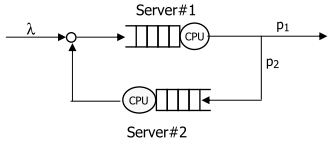
\includegraphics[scale=1]{figures/ex/jksnet.png}
\caption{Jackson Network}
\end{figure}
\end{center}

Si assuma che i singoli intervalli di tempo durante i quali viene utilizzato la 
CPU del server\#1 ed i singoli intervalli di tempo durante i quali viene 
utilizzata la CPU del server\#2 siano descritti da variabili casuali indipendenti 
e distribuite esponenzialmente a valor medio, rispettivamente, $\frac{1}{\mu_1}$ e $\frac{1}{\mu_2}$.  
Si assuma, inoltre, che i sistemi a coda in figura abbiano una capacità 
illimitata ed una disciplina di servizio di tipo FCFS.  
Si calcoli: 

\begin{itemize}
\item{a)} Il fattore di utilizzazione della CPU del server\#1; 
\item{b)} il valore medio del tempo di esecuzione di un job, a regime; 
\item{c)} il valore medio del tempo totale di CPU del server\#1 richiesto da un job, a 
regime; 
\item{d)} il valore medio del tempo totale di CPU del server\#2 richiesto da un job, a 
regime.

\end{itemize}

Risoluzione:

($\lambda$-POISSON) processi degli arrivi. $p_1$ che il job sia eseguito; $p_2=1-p_1$ che utilizzi il server 2. Se il job utilizza il server 2 ritorna in feedback all'ingresso di "1". $\{\{\lambda\},\{\mu_1,\mu_2\}\}$. $(d=+\infty)$, FCFS. Ci troviamo dinanzi una JN con code $\mathord{\cdot}$/M/1. Ma potrebbero anche essere \{$\mathord{\cdot}$/M/m, $\mathord{\cdot}$/M/$\infty$\}. M/M/1 in isolamento ai fini della OD. Definiamo con $\lambda_1$ velocità totale di arrivo dei clienti al nodo "1". Analogamente per "2", con $\lambda_2$. Applicando le equazioni del traffico troviamo:

\[
	\left\{
	\begin{aligned}
	&\lambda_1=\lambda+\lambda_2\\
	&\lambda_2=\lambda_1 p_2
	\end{aligned}
	\right. \implies \left\{
	\begin{aligned}
	&\lambda_1=\frac{\lambda}{1-p_2}\\
	&\lambda_2=\frac{\lambda}{(1-p_2=p_1)}p_2
	\end{aligned}
	\right.
\]

Dobbiamo imporre le Stabilità dei sottosistemi: $\implies$

\[
	\left\{
	\begin{aligned}
	&[\underline{\rho_1=\frac{\lambda_1}{\mu_1} = \frac{\lambda}{p_1\mu_1}}] < 1\\
	&[\underline{\rho_2=\frac{\lambda_2}{\mu_2} = \frac{\lambda p_2}{p_1\mu_2}}] < 1
	\end{aligned}
	\right.
\]

ove i termini sottolineati rappresentano il fattore di utilizzazione del server 1 e quello del server 2, rispettivamente. \underline{Little}. $\bar{N}=\bar{N}_1+\bar{N}_2$. Dove:

\[
	\left\{
	\begin{aligned}
	&\bar{N}_1 = \frac{\lambda_1}{\mu_1-\lambda_1} = \frac{\lambda}{p_1(\mu_1-\frac{\lambda}{p_1})} = \frac{\lambda}{p_1\mu_1-\lambda}\\
	&\bar{N}_2 = \frac{\lambda_2}{\mu_2-\lambda_2} = \frac{\lambda p_2}{p_1(\mu_2-\frac{\lambda p_2}{p_1})} = \frac{\lambda p_2}{p_1\mu_2-\lambda p_2} = \frac{\lambda}{\frac{p_1}{p_2}\mu_2-\lambda}
	\end{aligned}
	\right.
\]

Ricordiamo che $\lambda$ è la velocità totale di arrivo dei clienti dall'esterno. Dobbiamo quindi applicare Little: $\implies$ 

\[
	\bar{R} = \frac{\bar{N}_1+\bar{N}_2}{\lambda} = (\frac{1}{p_1\mu_1-\lambda} + \frac{1}{\frac{p_1}{p_2}\mu_2-\lambda})
\]

Quindi questo è il tempo medio di risposta. Dal punto di vista del tempo medio di risposta = tempo medio di permanenza, vi è un'equivalenza a due M/M/1 posti in serie, con velocità di servizio rispettivamente $\mu_1'=p_1\mu_1$ e $\mu_2'=\frac{p_1}{p_2}\mu_2$. RITARDO MEDIO il MEDESIMO, ma la distribuzione $\Pr\{R\leq t\}$ è DIFFERENTE!!

Calcoliamo le Service demand per i due nodi:

\[
	\left\{
	\begin{aligned}
	&D_1 = (\frac{1}{\mu_1}){(e_1=\frac{\lambda_1}{\lambda})} = \frac{1}{\mu_1} \frac{\lambda_1}{\lambda} = \frac{1}{\mu_1} \frac{\lambda}{p_1 \lambda} = \frac{1}{\mu_1 p_1}\\
	&D_2 = (\frac{1}{\mu_2})(e_2=\frac{\lambda_2}{\lambda}) = \frac{1}{\mu_2}\frac{\lambda p_2}{p_1}\frac{1}{\lambda} = \frac{1}{\mu_2}\underline{\frac{p_2}{p_1}}
	\end{aligned}
	\right.
\]

Dove $e_i$ rappresenta il numero medio di visite dall'esterno al nodo "i". Nel caso "2" ad esempio, il termine sottolineato indica $e_2 = \frac{p_2}{p_1}$. Notiamo che il nodo "1" verrà visitato sempre una volta in più prima di lasciare la rete: $+1 \implies \frac{p_2}{p_1}+1 = (\frac{1}{p_1})$. Potrei considerare: $\xi$ il numero totale di visite al server 1. $i-1$ volte visiti il nodo "2", e la volta successiva il cliente lascia la rete. Se $p_1=\Pr\{si\ lasci\ la\ rete\}$, allora vale:

\[
	\E[\xi] = \sum_{i=1}^{+\infty}{i\Pr\{\xi=i\}} = \sum_{i=1}^{+\infty}{ip_2^{i-1}p_1} =
\]
\[
	= p_1\sum_{i=1}^{+\infty}{ip_2^{i-1}} = p_1 \frac{1}{(1-p_2)^2} = p_1 \frac{1}{p_1^2} = \underline{\frac{1}{p_1}}
\]

(INDEPENDENT BERNOULLI TRIALS).


\subsection{Reti BCMP}

Reti di code \{CICLICHE, ACICLICHE, JACKSON\}. Per queste tipologie di code si ha una sola classe di clienti. Rete dati modellabile come rete di code, ma bisognerebbe differenziare le varie classi! $p_{ij} = \mathord{\cdot}(stream\ di\ pacchetti)$. Indici di prestazioni: \{ritardo medio\}. \underline{Reti di code BCMP} e teorema \underline{BCMP}. Va a definire una classe di reti di code per le quali vale ancora la Soluzione in forma prodotto per la Occupancy Distribution. Ma in questo caso i fattori del prodotto non corrispondono necessariamente alle distribuzioni marginali. Ma i fattori si ottengono a partire dall'analisi dei vari sistemi a coda visti in isolamento. Le BCMP comprendono le reti di JACKSON e quindi anche le ACICLICHE. C'è la possibilità di avere più classi di clienti $R$.

\begin{itemize}

\item{-)} $R=\cardinality{classi}$. Le classi possono essere APERTE o CHIUSE.

\begin{itemize}

\item{\textbf{APERTE}}: i clienti al loro interno possono partire dall'esterno ed arrivare dall'esterno;
\item{\textbf{CHIUSE}}: altrimenti
\end{itemize}

La BCMP è detta \textit{MIXED} se alcune classi sono aperte ed altre chiuse;

\item{-)} class switching possibile. Possibile che un cliente appartenente ad una certa classe, partendo da un nodo, visiti un certo nodo cambiando la sua classe;
\item{-)} $N=\cardinality{nodi}$. $p_{ir,js},\ r,s=1,2,\ \dots,\ (R=\cardinality{classi}),\ i,j=1,2,\ \dots,\ N=\cardinality{nodi}$ di reti di code. Si definirà quindi una \textit{matrice di routing}:

\begin{defn}{\textbf{Matrice di Routing}}

Per indicare le probabilità che un cliente appartenente ad una certa classe, partendo da un nodo, visiti un certo nodo cambiando la sua classe, si definisce:

\[
	\underline{\underline{P} := [p_{ir,js}]}
\]

\end{defn}

Tipicamente è una matrice SPARSA. A rigore sarebbe in realtà un tensore quadridimensionale. Se togliamo il class switching il tensore si ridurrebbe a 3 dimensioni.

\item{-)} Per quanto concerne la disciplina di coda, sino ad adesso abbiamo visto la FCFS, adesso ne sono consentite altre: \{\{PS, LCFS-PR, IS\}, FCFS\}. Ne spieghiamo qualcuna:

\begin{itemize}

\item{\textbf{PS} = \textit{processor sharing}}: \underline{tutti i clienti sono serviti contemporaneamente}, con time slicing;
\item{\textbf{LCFS-PR} = \textit{Last-Come-First-Served with Preemptive-Resume}}: Se un cliente viene servito ed arriva un altro cliente, vi è l'interruzione del servizio corrente ed il cliente corrente va in fila di attesa. Rientrerà nel servizio quando $\nexists$ clienti nel sistema a coda;
\item{\textbf{IS} = \textit{Infinite Server}}: Come suggerisce lo stesso nome, prevede INFINITI $(\infty)$ servitori! $\iff (m=+\infty)$ Come nell'M/M/$\infty$.

\end{itemize}

\end{itemize}

Vi è un'altra differenza (caratteristica aggiuntiva) riguardo la distribuzione dei tempi di servizio. Fino ad adesso abbiamo visto la distribuzione esponenziale. Adesso è permessa qualsiasi distribuzione purché la trasformata di Laplace della PDF sia razionale. COX ha dimostrato che qualunque distribuzione di v.a. si può approssimare sufficientemente bene mediante le seguenti reti di stadi: abbiamo una Rete di Stadi esponenziali. Il tempo di permanenza di un cliente in $\mu_i$ è distribuito esponenzialmente. Possiamo associare delle variabili casuali $\{\eta_1,\eta_2,\ \dots,\ \eta_n\}$ che sono tutte distribuite esponenzialmente $\iff \eta_i \sim EXP(\mu_i)\ \forall i=1,\ \dots,\ n$, ed indicano il tempo di permanenza in ciascuno stadio $i$-esimo. $\{a_i,b_i\}$ sono delle probabilità. La distribuzione associata all'attraversamento (al tempo di attraversamento) dell'intero sistema si chiama \textit{distribuzione di COX} e mediante essa possiamo approssimare (giocando opportunamente con il numero di stadi) sufficientemente bene una qualsiasi distribuzione. A questo punto il vincolo della trasformata di Laplace razionale della PDF non è più limitativo dal momento che la distribuzione di COX ha una TL della PDF razionale (PDF associata alla v.a. tempo di attraversamento).

Quindi possiamo pensare ad un unico servitore che rappresenti tutto il sistema. Il servitore è unico! Il servizio parte quando entra nel sistema e finisce quando il cliente esce dall'ultimo stadio. Solo alla fine un altro cliente va al servizio. In alcuni casi è ammessa una velocità del servizio che dipenda dal numero di clienti nella coda (M/M/m), o dal numero di clienti di una CERTA CLASSE nella coda.

(Probabilità di routing). La disciplina NON è a priorità! Ancora non la stiamo esaminando (interruzioni e senza interruzioni). Per queste reti che prevedono le forme prodotto NON è possibile.
Consideriamo il caso di rete BCMP aperta (\textit{OPEN-BCMP}). Vediamo che i processi degli ARRIVI sono ammesssi in questa rete. Consideriamo due casi, due possibilità:

\begin{itemize}

\item{\textit{\underline{CASO 1}}}: i clienti arrivano alla rete da un'unica sorgente, con tempi di interarrivo indipendenti e distribuiti esponenzialmente. Il Rate di arrivi $(\lambda)$ può dipendere dal numero di clienti $K$ nella rete $\iff \lambda=\lambda(K)$. \underline{Se $[\lambda\neq\lambda(K)]$} (si riferisce al rate di arrivo), \newline
\underline{avremo un processo di POISSON omogeneo}. Un cliente in arrivo visiterà il nodo $i$ in classe $r$ con probabilità $p_{0,ir}$ (giungendo dall'esterno). Ovviamente dovrà valere il seguente vincolo:

\[
	[\sum_{i=1}^N{\sum_{r=1}^R{p_{0,ir}=1}}]
\]

\item{\textit{\underline{CASO 2}}}: Se non facessi delle semplificazioni dovrei trattare delle sottocatene di Markov ergodiche. Eviteremo quindi il class switching. Supponiamo che non vi sia CS quindi. In tal caso si ha un processo degli arrivi $\forall$ classe di clienti. La velocità di arrivo $\lambda_r$ (indicizzata su $r$) potrà dipendere da $K_r \implies \lambda_r=\lambda_r(K_r),\ r=1,2,\ \dots,\ R$. Se $\lambda_r\neq\lambda_r(K_r)$ avremo un processo di POISSON omogeneo per la classe $r$.
\end{itemize}

Con le BCMP si può benissimo modellare un \textit{J2EE}, con Studio di Affidabilità e Disponibilità annesso. Quindi nel \underline{primo} caso abbiamo un unico processo degli arrivi, mentre nel \underline{secondo caso} non abbiamo class switching ed abbiamo un processo degli arrivi differente $\forall$ classe della rete. $K_r=\cardinality{clienti\ della\ classe\ r}$. Tipi di nodi ammessi nella BCMP: Nodi: \{\underline{type 1}, \underline{type 2}, \underline{type 3}, \underline{type 4}\}.

\begin{itemize}

\item{\underline{type 1}}: FCFS node. Coda con tempi di servizio distribuiti esponenzialmente con lo stesso valor medio (SAME $\frac{1}{\mu_i}$) per tutte le classi. La velocità di servizio $(\mu_i)$ può dipendere dal numero di clienti totali nella coda (nel sistema a coda). LOAD DEPENDENT SERVICE-RATE (LDSR) possibile. Può servire per modellare dispositivi I/O, HDD. Lo utilizzeremo per modellare tempi di accodamento e trasmissione dei router. Considereremo quindi: \{$\mathord{\cdot}$/M/$m_i$, \underline{FCFS}\};

\item{\underline{type 2}}: PS node (processor sharing). Utilizzato per modellare le CPU. Code con servitore unico e disciplina PS. Tutti i clienti sono serviti contemporaneamente. Sono possibili distribuzioni dei tempi di servizio diverse per classi diverse. Differenza rispetto al type 1. E qui non ci deve essere per forza l'esponenziale \{\underline{DSD} for \underline{DSC}\}. Vale sempre il vincolo sulle TL della PDF dei tempi di servizio. La velocità di servizio per una classe può dipendere dal numero di clienti nel nodo od anche dal numero di clienti di quella classe nel nodo. (Anche qui LDSR possibile);

\item{\underline{type 3}}: Detto IS (\textit{Infinite Server}) node oppure \textit{Delay Node}, perché solitamente utilizzato per modellare il ritardo (ritardo di elaborazione). Tutto quello scritto per il \underline{type 2} vale anche per il \underline{type 3}. Code del tipo: $\mathord{\cdot}$/G/$\infty$. Sempre un servitore a disposizione. In fila di attesa NON c'è mai nessuno. (Infiniti servitori $\implies \nexists$ fila di attesa). \`E come se non ci fosse alcuna disciplina;

\item{\underline{type 4}}: LCFS-PR (LCFS with Preemptive Resume). Coda con un unico servitore con quella disciplina di servizio. Contempliamo quindi le \{$\mathord{\cdot}$/G/1 - LCFS-PR\}. Unico servitore con quella disciplina di coda.

\end{itemize}

\subsubsection{Teorema BCMP}

Andiamo direttamente ad una versione semplificata del teorema BCMP (\textit{Baskett, Chandy, Muntz and Palacios}). Versione semplificata. Serve per modellare le reti di dati. Consideriamo BCMP (reti di code) aperte con load independent arrival rate. Quindi sostanzialmente processi di arrivo omogenei. Reti BCMP aperte con $[\lambda\neq\lambda(K)] \implies$ processi degli arrivi omogenei sostanzialmente.

Consideriamo che le velocità di servizio siano tali che $[\mu_i\neq\mu_i(K)]$. Casi ovviamente estendibili. Consideriamo:

\[
	\left\{
	\begin{aligned}
	&N=\cardinality{nodi}\\
	&R=\cardinality{classi}\\
	&K_i=\cardinality{clienti\ totali\ nel\ nodo\ i}\\
	&K_{ir}=\cardinality{clienti\ di\ classe\ r\ nel\ nodo\ i}\\
	&\underline{K}=(K_1,K_2,\ \dots,\ K_N)\\
	&\left\{
	\begin{aligned}
	&K_i=\sum_{r=1}^R{K_{ir}}\\
	&K=\sum_{i=1}^N{K_i} = \sum_{i=1}^N{\sum_{r=1}^R{K_{ir}}}
	\end{aligned}
	\right.
	\end{aligned}
	\right.
\]

Con queste quantità, la Occupancy Distribution è uguale a:

\[
	\Pr\{\underline{K}\} = \pi(K_1,K_2,\ \dots,\ K_N) = \prod_{i=1}^N{\pi_i(K_i)}
\]

questa è la OD per questa OPEN-BCMP. $\pi_i(K_i)$ è caratterizzato in questo modo:

\[
	\pi_i(K_i) = \left\{
	\begin{aligned}
	&\underline{(1-\rho_i)\rho_i^{K_i}},\ type\ 1,\ type\ 2,\ type\ 4\\
	&\e^{-\rho_i}\frac{\rho_i^{K_i}}{K_i!},\ type\ 3
	\end{aligned}
	\right.
\]

Per quanto concerne l'equazione che presenta il termine sottolineato, è bene specificare che abbiamo una restrizione sul type 1: è necessario avere esclusivamente un unico servitore ($\underline{m_i=1\ \forall i}$). La formula ricorda tanto la M/M/1. Ma vale anche per type (1,2,4). Reti: $\mathord{\cdot}$/M/$(1=m_i)$. Per la terza invece abbiamo reti $\mathord{\cdot}$/G/$\infty$. $\rho_i$ è il fattore di utilizzazione del nodo $i$. Vale: $\rho_i := \sum_{r=1}^R{\rho_{ir}}$. ($\forall$ classe di servizio), Se ho $m_i$ servitori nel type 1, $\pi_i(K_i)$ avrà la stessa espressione trovata per la M/M/$m_i$ $(\lambda_i,\mu_i)$. Le velocità di arrivo le calcoliamo con le \underline{EQUAZIONI DEL TRAFFICO}. Considerando $(m_i=1)$, dobbiamo imporre che $(\rho_i<1)$ per la STABILIT\`A della CODA. Anche per il type 1 con più servitori $(m_i\geq 1)$, avremo: $\rho_i=\frac{\lambda_i}{m_i\mu_i}$ nel caso $m_i\geq 1$. Quindi:

\[
	\rho_{ir} = \left\{
	\begin{aligned}
	&\frac{\lambda_{ir}}{\mu_i},\ type\ 1,\ \mu_i\neq\mu_{ir}\\
	&\frac{\lambda_{ir}}{\mu_{ir}},\ type\ \{2,3,4\},\ (\mu_i=\mu_{ir}) = \mathord{\cdot}(IDX\ r)
	\end{aligned}
	\right.
\]

Nel secondo caso infatti (seconda equazione), le distribuzioni dei tempi di servizio possono essere differenti per le varie classi. Ricordiamo che vale: $[\underline{\lambda_i}=\sum_{r=1}^R{\lambda_{ir}}]$, differenziando ed includendo rispetto alle varie classi.  Il termine sottolineato rappresenta la velocità \underline{totale} di arrivo al nodo $i$.

\subsection{RECAP}

[BCMP $\supset$ JACKSON $\supset$ ACICLICHE]. $\pi_i(K_i)$, reti \{$\mathord{\cdot}$/M/1, $\mathord{\cdot}$/G/1-PS, $\mathord{\cdot}$/G/1-LCFS-PR\}. Per queste code, ai fini dell'Occupancy Distribution, si comportano come se fossero delle M/M/1 in isolamento ($1=m_i$ servitori $\forall i$). Nel type 1 abbiamo la FCFS, mentre nel type 2, type 4 non abbiamo quella disciplina di coda! \`E come se ai fini del calcolo della OD, avessimo invece proprio la disciplina FCFS. Si comportano proprio come se fossero M/M/1 in isolamento.

Per quanto riguarda il secondo caso, per un M/M/$\infty$ abbiamo $[\e^{-\rho_i}\frac{\rho_i^{K_i}}{K_i!}]$. Ma vale sostanzialmente per tempi di servizio non distribuiti esponenzialmente (per le $\mathord{\cdot}$/G/$\infty$). La motivazione è collegata proprio al teorema BCMP. Tornando al primo caso, ipotizziamo una rete di code BCMP con un processo degli arrivi dall'esterno che NON dipenda dal carico (Stiamo considerando un processo degli arrivi di POISSON omogeneo). Il BCMP vale anche se c'è un solo sistema a coda! Consideriamo $\mathord{\cdot}$/M/1. Adesso sono sicuro che mi trovo dinanzi una M/M/1. Adesso i processi degli arrivi sono di POISSON. Per il \underline{type 2}, M/G/1-PS. Stesso discorso per il \underline{type 4}. Le formule trovata per un M/M/1, sono valide anche per un \{\underline{M/G/1-PS}, {M/G/1-LCFS-PR}\}, ove i termini sottolineati si riferiscono rispettivamente a code del tipo \underline{type 2} e \underline{type 4}.


\section{Reti di dati}

Ulteriore passaggio verso la modellazione. Obiettivo: modellare una rete di dati switched. Consideriamo $(i\rightarrow j)$. Ci saranno 4 componenti di ritardo su questo link. Dobbiamo considerare:

\begin{itemize}

\item{-)} tempi di accodamento in $i$;
\item{-)} tempi di trasmissione su questo link;
\item{-)} tempi di propagazione;
\item{-)} tempi di elaborazione

\end{itemize}

Modellando queste componenti di ritardo per il link $(i\rightarrow j)$, consideriamo nel primo blocco sicuramente $\mathord{\cdot}$/M/1 e agli ultimi due blocchi utilizzeremo rispettivamente: \{$\mathord{\cdot}$/G/$\infty$ e $\mathord{\cdot}$/G/$\infty$\}.
I sistemi a coda sono dei modelli per modellare il ritardo.

Virtual Circuit (a commutazione di pacchetto). Per un certo flusso la ROTTA sarà sempre la stessa. Stiamo immaginando qui di avere 3 flussi: $\{X_{s1}, X_{s2}, X_{s3}\} \leftarrow$ velocità di arrivo. Per il link $(i\rightarrow j)$ abbiamo il flusso di pacchetti $s_1-s_2 \implies X_{s_{i-j}} = X_{s1}+X_{s2}$. A questo punto, per valutare $\lambda_{ij}$, dobbiamo trovare la somma delle $X_s$ estesa a tutti gli stream $S$ che attraversano il link $(i\rightarrow j)$:

\[
	[\underline{\lambda_{ij}} = \sum_{stream\ s\ in\ (i,j)}{X_s}]
\]

$X_{si}$ è il rate (velocità) del flusso $i$-esimo. La rete Internet è a commutazione di pacchetto ma di tipo Datagram (Rotte non sempre le stesse). Per le DATAGRAM: $f_{ij}(s_1)X_{s,1}$ rappresenta la Velocità di arrivo, considerando le opportune frazioni dei pacchetti. Qui per calcolare le velocità di arrivo totale dobbiamo considerare le seguenti formule:

\[	
	\underline{\lambda_{ij}} = \sum_{stream\ s\ in\ (i,j)}{f_{ij}(s)X_s}
\]

ove la somma è estesa al solito a tutti gli stream che attraversano il link $(i\rightarrow j)$. Biforcazione o fork possibile.

Velocità di arrivo totale dei vari link sia su una VC che su una DATAGRAM. Entrambe a commutazione di pacchetto. Rete di code BCMP. Versione semplificata del teorema per modellare una rete di dati come una rete di code. Modellare ogni link della rete con il seguente schema:




Ipotesi sul sistema reale. Rete BCMP (più flussi) $\implies$ ($\forall$ flusso $\exists$ classe associata ad esso $\iff (s\rightarrow r)$). Sia $R=\cardinality{flussi\ di\ pacchetti}$. Rete BCMP con $R$ classi di clienti. Consideriamo il generico flusso $s$, al quale corrisponde una certa velocità $X_s \impliedby (s\rightarrow X_s)$. Per quanto concerne le velocità totali abbiamo: $\underline{\lambda_{0,r}}$ è la velocità di arrivo dall'esterno dei clienti di classe $r$; $\lambda_{0,hr}$ è la velocità di arrivo dall'esterno dei clienti di classe $r$ alla coda di ingresso $h$ della rete; $p_{0,hr}$ è la probabilità che un cliente dall'esterno di classe $r$ vada verso la coda $h$. Immaginiamo che $h$ sia il nodo di ingresso $\implies p_{0,hr}=1$:

\[
	X_s=\lambda_{0,r} \impliedby [\lambda_{0,r}p_{0,hr} = \underline{\lambda_{0,hr}}]
\]

Difatti quella probabilità è 1 per quella coda che rappresenta il nodo di ingresso. $\nexists$ biforcazioni all'ingresso della rete. Per applicare il teorema BCMP dovremo imporre che questi pacchetti arrivino secondo un processo di POISSON. Un'altra ipotesi riguarda i tempi di trasmissione. Nel primo blocco modelliamo il ritardo di accodamento e quello di trasmissione. Dobbiamo ipotizzare che i tempi di trasmissione siano distribuiti esponenzialmente (Con la stessa distribuzione per tutte le classi). Parametro $(\frac{1}{\mu_{ij}})$ come valor medio. Supponiamo che i buffer del router siano molto grandi $(d=+\infty)$ da poter ritenersi illimitati. Valga l'approssimazione di Kleinrock. Indipendenza tra i tempi di interarrivo e tempi di servizio. (Reti magliate ed intensità di traffico medio-alta). Vale quando la rete è abbastanza magliata e intensità di traffico medio-alta. Con queste ipotesi possiamo applicare il teorema BCMP. I due successivi blocchi di ritardo modellano il tempo di propagazione e di elaborazione (quest'ultimo è il router $j$) (ADN). Per elaborazione si intende il ritardo per decidere il routing. Il router analizzerà i vari link e si occuperà di decidere consultando le tabelle di forwarding. Il tempo di propagazione si trascura solitamente. Al posto dell'$\mathord{\cdot}$/M/1 andrebbe bene un $\mathord{\cdot}$/M/$\infty$. Anche se non siamo vicini alla distribuzione esponenziale per le lunghezze dei pacchetti, tutto alla fine va ancora bene. Applichiamo quindi le formule BCMP. Sia: $\bar{R}$ il tempo medio di attraversamento della rete da parte di un pacchetto. \underline{POOLING} di tutti i flussi che attraversano lo stesso link. Abbiamo: $\bar{R}=\frac{N}{\gamma}$, ove abbiamo posto $\gamma:=\sum_{tutti\ gli\ stream\ s}{X_s}$ ovvero la velocità totale di arrivo dei pacchetti. Dato che abbiamo a che fare con valor medi... indichiamo inoltre con \{$\E[T_{ij}^p],\ \E[T_{ij}^e]\}$ rispettivamente il valor medio del tempo di propagazione ed il valor medio del tempo di elaborazione, entrambi sul link $(i\rightarrow j)$. Sfruttando le formule dell'M/M/1 e di Little otteniamo:

\[
	\bar{N}_{ij} = \frac{\lambda_{ij}}{\mu_{ij}-\lambda_{ij}} + \lambda_{ij}\E[T_{ij}^p] + \lambda_{ij}\E[T_{ij}^e]
\]

Abbiamo trovato il numero medio di pacchetti sul link $(i,j) \implies \bar{N}=\sum_{(i,j)}{\bar{N}_{ij}}$. Dividiamo per la velocità totale di arrivo dei pacchetti $(\gamma)$ e troviamo $\bar{R}$. Sempre per il fatto della forma prodotto. (M/M/1) in isolamento (BCMP TH.). Se introduco un modello M/G/$\infty$, un po' di errore lo commetto. Le formule che ottengo per l'M/G/$\infty$ sono analoghe a quelle M/M/$\infty$.

\begin{thrm}{\textbf{$\bar{R}_{path}$}}

Per calcolare questa quantità, dovrei considerare tutti i link associati a questo percorso:

\[
	\bar{R}_{path} := [\sum_{link(i,j)\ lungo\ path}{\frac{1}{\mu_{ij}-\lambda_{ij}}}] + \E[T_{ij}^p + \E[T_{ij}^e]]
\]

\end{thrm}

Vale per tutte le classi! $(\forall r=s)$. Qualunque sia la sua classe. Tanto è inglobata nelle varie quantità $(\mu_{ij},\ \lambda_{ij})$. 


\subsection{Exercise}

Consider the network in the figure below. There are four sessions: ACE, ADE, BCEF and BDEF 
sending Poisson traffic at rates $\{100,\ 200,\ 500,\ 600\}\ pkt/min$, respectively. Packets lengths are 
exponentially distributed with mean $1000\ bits$. All transmission lines have capacity $50\ kbits/s$, 
and there is a propagation delay of $2\ msec$ on each line. Using the Kleinrock independence 
approximation, 

\begin{itemize}

\item{a)} find the average number of packets in the system, the average delay per packet (regardless of 
session) and the average delay per packet of each session; 
\item{b)} derive the CTMC that can be used to find the approximate delay distribution related to the 
packets belonging to the ACE session

\end{itemize}

\begin{center}
\begin{figure}[H]
\centering
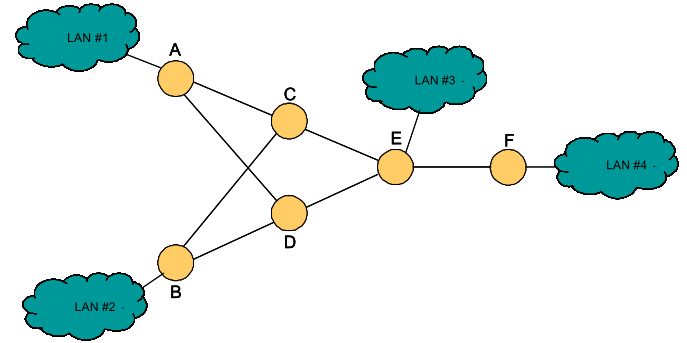
\includegraphics[scale=0.8]{figures/ex/mdn.png}
\caption{Data Network}
\end{figure}
\end{center}

Flussi in realtà bidirezionali. Ma a livello didattico concentriamoci nel caso NON DUPLEX ($\iff$ Flussi unidirezionali). Abbiamo varie sessioni:

\[
	\left\{
	\begin{aligned}
	&ACE, 1\\
	&ADE, 2\\
	&BCEF, 3\\
	&BDEF, 4
	\end{aligned}
	\right.
\]

Quattro servizi che generano pacchetti alle seguenti velocità. $\{100,200,500,600\}\  [pkt/min]$. $\mathit{L}=1000\ bit$ (lunghezza pacchetti), $C=50\ kbps$. $\E[T_{ij}^p]=dp=2ms$ (propagation delay, PD). ($\forall ij$. Qualunque sia il link $i,j$). Il PD è in realtà una costante, non un valor medio. Supponiamo quindi che tutti i link siano alla stessa velocità. Supponiamo valida l'approssimazione di Kleinrock. 4 flussi di pacchetti $\iff$ 4 sessioni di comunicazioni. Numeriamo le sessioni e calcoliamo:

\[
	\left\{
	\begin{aligned}
	&X_1 = (\frac{100}{60} = \frac{5}{3})\ pkt/s\\
	&X_2 = (\frac{200}{60} = \frac{10}{3})\ pkt/s\\
	&X_3 = (\frac{500}{60} = \frac{25}{3})\ pkt/s\\
	&X_4 = (\frac{600}{60} = 10)\ pkt/s
	\end{aligned}
	\right.
\]

Ci serve andare a calcolare le velocità totali di arrivo sui VARI link attraversati. 

\[
	\left\{
	\begin{aligned}
	&\lambda_{AC}=X_1\\
	&\lambda_{CE}=X_1+X_3=10\ pkt/s\\
	&\lambda_{AD}=X_2\\
	&\lambda_{BD}=X_4=10\ pkt/s\\
	&\lambda_{DE}=X_2+X_4=\frac{40}{3}\ pkt/s\\
	&\lambda_{BC}=X_3\\
	&\lambda_{EF}=X_3+X_4=\frac{55}{3}\ pkt/s
	\end{aligned}
	\right.
\]

Dobbiamo andare a considerare la velocità di servizio su ogni link. Ci troviamo dinanzi $\mathord{\cdot}$/M/1. Ma anche relativi ai router dei blocchi $\mathord{\cdot}$/G/$\infty$. Dividiamo $\frac{C}{\mathit{L}}=\mu_{ij}=(\frac{50000}{1000}=50)\ pkt/s$. Dobbiamo calcolare il $\gamma$ (velocità totale di arrivo dei clienti):

\[
	\gamma=\sum_{i=1}^4{X_i}=\frac{70}{3}\ pkt/s
\]

in quanto abbiamo 4 flussi diversi. Con $\bar{N} \simeq 1.84\ pkt$ pacchetti, abbiamo quindi:

\[
	\bar{R}=\frac{\bar{N}}{\gamma}=\frac{1.84}{70/3\ pkt/s} = \frac{3(1.84)}{70} msec\ (millisec)
\]

(poco credibile oggi). Dobbiamo ora calcolare il ritardo medio $\forall$ stream (per i vari stream). Per le varie sessioni ($\bar{R}_{path}$ formula), abbiamo:

\[
	\bar{R}_p=[50ms,\ 53ms,\ 87ms,\ 90ms]
\]

$\Pr\{R\leq t\}$, dove $R$ è il ritardo, tempo di attraversamento della rete.

Distribuzione del ritardo. Supponiamo di voler determinare la distribuzione del ritardo dei pacchetti associati alla sessione ACE. CMTC che con uno stato assorbente può essere utilizzata per modellare il ritardo $(ACE=AC+CE)$ (link attraversato):



Distribuzione di ritardo = tempo di permanenza di un pacchetto nella rete in questione. Abbiamo trascurato i ritardi di elaborazione. $\mathord{\cdot}$/M/1, che tiene conto dei ritardi di accodamento + il ritardo di trasmissione. Presso il nodo "C" arriveranno pacchetti anche dal nodo "B" (da un altro stream) (BCEF). Determinare la distribuzione del tempo di risposta in una rete di code aperta. C'è un metodo per approssimare questa distribuzione (del tempo di risposta), e si basa sulla conoscenza della distribuzione del tempo di risposta relativa ai vari sottosistemi di cui la rete si compone. Reti di code di JACKSON. Tempo di risposta = tempo di attraversamento. Vogliamo approssimare questa distribuzione (del tempo di risposta). \`E possibile andare a derivare da questa rete di JACKSON una CMTC con \underline{stato assorbente}. Il \underline{time-to-absorption} (la sua distribuzione), rappresenta un'approssimazione del tempo di risposta della rete. Se è ACICLICA (rete di JACKSON senza CICLI) si ha una coincidenza tra TTA e tempo di risposta della rete.
Consideriamo questa rete CICLICA:

\begin{center}
\begin{figure}[H]
\centering
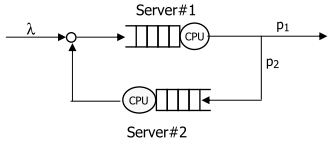
\includegraphics[scale=1]{figures/ex/jksnet.png}
\caption{Jackson Network}
\end{figure}
\end{center}

Due $\mathord{\cdot}$/M/1. Questo metodo si basa sulla conoscenza delle distribuzioni dei vari tempi di risposta dei singoli sottosistemi di cui si compone la rete. M/M/1. $R$ = tempo di permanenza. Sappiamo che: $R \sim EXP(\mu-\lambda)$. $F(t)\ CDF$, quindi la CDF del tempo di risposta in un M/M/1 è:

\[
	F(t)=\Pr\{R\leq t\} = 1-\e^{-(\mu-\lambda)t}
\]

Sulla base di queste conoscenze, possiamo dedurre, ricavare la seguente CMTC:

\begin{center}
\begin{tikzpicture}[->, >=stealth', auto, semithick, node distance=3cm]
\tikzstyle{every state}=[fill=white,draw=black,thick,text=black,scale=1]
\node[state]    (1)                     {$1$};
\node[state]    (2)[right of=1]   {$2$};
\node[state]    (C)[below of=1]   {$C$};
\path
(1) 
    edge[bend left]     node{$(\mu_1-\lambda_1)p_2$}     (2)
    edge[bend right,left]    node{$(\mu_1-\lambda_1)p_1$}      (C)
(2) edge[bend left]                node{$(\mu_2-\lambda_2)\underline{1}$} (1);
\end{tikzpicture}
\end{center} 

con: $\{\{C\},\{1,2\}\}$ rispettivamente come Stato assorbente e Stati transitori. Lo STARTING STATE è lo stato 1, ovvero lo stato dalla quale evolve la CMTC. $R\sim EXP(\mu-\lambda)$. Rappresenta la permanenza del cliente sul sistema. Tempo di permanenza di un determinato cliente. In particolare, il tempo di soggiorno della CMTC in questo stato corrisponde al tempo di permanenza nel primo M/M/1. ($R_1\sim EXP(\mu_1-\lambda_1)$). Il tempo di soggiorno della catena nello stato 2 rappresenta il tempo di permanenza del cliente nel sistema nel sistema a coda 2 ($R_2\sim EXP(\mu_2-\lambda_2)$). Se invece lasciasse la rete, si avrebbe una transizione verso lo stato assorbente \{C\}. Il TTA qui corrisponde al ritardo del cliente in questa rete (tempo di permanenza). Se riesco a determinare la distribuzione del TTA per questa catena riesco a determinare proprio il tempo di permanenza nella mia rete. Ma è un'approssimazione questa, in quanto abbiamo dei cicli! Quindi i processi degli arrivi NON sono di POISSON. 

\[
	\underline{\Pr\{T_a\leq t\}} \simeq \underline{\Pr\{R\leq t\}}
\]

ove il LHS sottolineato rappresenta $\pi_C(t)$ in TRANSITORIO, mentre il RHS sottolineato rappresenta la distribuzione del ritardo nella mia rete. A quanto pare vi è un'approssimazione possibile. Per trovare $\pi_C(t)$ si può procedere con il metodo della trasformata di Laplace, diversamente ci sono dei programmi di simulazione e non. Si richiami il concetto di affidabilità:

\[
	\Pr\{R>t\} = 1-\underline{\pi_0(t)} = 1-\Pr\{R\leq t\}
\]

\subsection{Response-Time Blocks (RTB)}

Li utilizziamo per trovare queste distribuzioni. Blocchi mediante i quali costruiamo le CMTC con stati assorbenti. Dobbiamo considerare tanti blocchi quante sono le componenti di ritardo.

\begin{itemize}

\item{\textbf{RTB \textit{M/M/1}}}: Ci sono quindi anzitutto quelle per la M/M/1 $(\lambda,\mu)$, ove per stabilità deve valere: $(\lambda<\mu)$. Il RTB per questo sistema è il seguente:

\begin{center}
\begin{tikzpicture}[->, >=stealth', auto, semithick, node distance=3cm]
\tikzstyle{every state}=[fill=white,draw=black,thick,text=black,scale=2]
\node[state]    (IN)                     {$IN$};
\node[state]    (OUT)[right of=IN]   {$OUT$};
\path
(IN) edge[bend left]     node{$(\mu-\lambda)$}     (OUT);
\end{tikzpicture}
\end{center}

Lo stato IN rappresenta il fatto che il cliente è entrato nella coda. Il tempo di soggiorno nello stato \{IN\} rappresenta il ritardo nella rete. \{OUT\} = \{partenza del cliente nella coda\}. (Tante serie di blocchi quanti sono i nodi in gioco):

\[
	\underline{F(t)} = 1-\e^{-(\mu-\lambda)t}
\]

Ove il termine sottolineato rappresenta la CDF del tempo di risposta. Lo stato \{OUT\} rappresenta la partenza del cliente. OUT nel precedente esercizio era \{2,C\}=OUT. In tali casi saranno da pesare le velocità di uscita complessive (con probabilità eventualmente, corrispondenti alle cosiddette probabilità di routing);

\item{\textbf{RTB \textit{M/M/$\infty$}}}: Il tempo di soggiorno nella mia catena corrisponde al tempo di servizio $\iff \nexists$ code nella M/M/$\infty$. (infiniti servitori, NO fila di attesa). 

\begin{center}
\begin{tikzpicture}[->, >=stealth', auto, semithick, node distance=3cm]
\tikzstyle{every state}=[fill=white,draw=black,thick,text=black,scale=2]
\node[state]    (IN)                     {$IN$};
\node[state]    (OUT)[right of=IN]   {$OUT$};
\path
(IN) edge[bend left]     node{$\mu$}     (OUT);
\end{tikzpicture}
\end{center}

Tempo di risposta corrisponde al tempo di servizio:

\[
	F(t) = \Pr\{R\leq t\}=1-\e^{-\mu t}
\]

\{IN\} rappresenta quindi lo stato di permanenza nel mio sistema;

\item{\textbf{RTB \textit{M/M/m}}}:

Per ultimo, ma non di importanza, abbiamo l'RTB di una M/M/m:

\begin{center}
\begin{tikzpicture}[->, >=stealth', auto, semithick, node distance=3cm]
\tikzstyle{every state}=[fill=white,draw=black,thick,text=black,scale=2]
\node[state]    (IN)                     {$IN$};
\node[state]    (OUT)[right of=IN]   {$OUT$};
\path
(IN) edge[bend left]     node{$\frac{\mu m (1-\rho)}{m(1-\rho)+C}$}     (OUT);
\end{tikzpicture}
\end{center}

ove $C$ è la C di ERLANG, ovvero la probabilità di accodamento;

\end{itemize}

Ma lo stato OUT può corrispondere allo stato IN di un altro blocco! Se effettivamente OUT è l'uscita della rete sarà assorbente, altrimenti NO.

Adesso consideriamo la rete precedente. Quella è la rete di code che modella la sessione ACE sostanzialmente:

\begin{center}
\begin{tikzpicture}[->, >=stealth', auto, semithick, node distance=3cm]
\tikzstyle{every state}=[fill=white,draw=black,thick,text=black,scale=1]
\node[state]    (A)                     {$A$};
\node[state]    (AC)[right of=A]   {$AC$};
\node[state]    (C) [right of=AC]                    {$C$};
\node[state]    (CE)[right of=C]   {$CE$};
\node[state]    (OUT)[right of=CE] {$OUT$};
\path
(A) edge[bend left]     node{$\mu-\lambda_AC$}     (AC)
(AC) edge[bend left]     node{$\frac{1}{d_AC}$}     (C)
(C) edge[bend left]     node{$\mu-\lambda_CE$}     (CE)
(CE) edge[bend left]     node{$\frac{1}{d_{CE}}$}     (OUT);
\node at ($(OUT)+(0,-0.8)$) {stato ASSORBENTE};
\end{tikzpicture}
\end{center}

Il nodo E interfaccia i pacchetti verso la LAN 3. (\underline{Rete ACICLICA}). Trascuriamo il ritardo di elaborazione, al solito. Velocità elevatissima! A volte si può ritenere legittimo trascurare il ritardo di accodamento e trasmissione della LAN di destinazione! Molto veloce! TTA in tal caso coincide esattamente con il ritardo di attraversamento (tempo di attraversamento) della rete, dal momento che la rete è ACICLICA.

%************************************************
% Chapter 5: NETWORK TECHNOLOGIES 2
%************************************************
% !TEX encoding = UTF-8
% !TEX TS-program = pdflatex
% !TEX root = ../nt.tex
% !TEX spellcheck = it-IT

%************************************************
\chapter{Network Technologies 2}
\label{cap:nt2}
%************************************************\\

\section{(Rapid)STP - Spanning Tree Protocol}

\{M/M/1, M/M/$\infty$\}. (STP)$\rightarrow$(RSTP) rapida. La RSTP (Rapid) è la versione veloce dell'STP. \`E un protocollo che consente di trasformare una topologia magliata in una ad albero (bridge). L'STP porta a dei tempi di convergenza molto elevati. \textit{IEEE 802.1D} è lo standard che va a definire i \textit{Transparent Bridge}. Oggi i bridge sono HW (lvl 2). Prima erano a livello SW. Oggi abbiamo i router HW ASIC elettronici (matrici ASIC).

L'STP serve per evitare che vi siano dei loop a lvl 2. Queste maglie esisteranno per via dei link ridondanti, introdotti per aumentare l'Affidabilità/Disponibilità. Dato che gli switch/bridge IEEE 802.1D non tollerano topologie magliate, allora serve l'STP. Il pericolo è quando loro fanno il flooding. Fase di forwarding, MAC Multicast/Broadcast $\implies$ flooding su tutte le altre porte. MAC Unicast $\implies$ funzioni di forwarding, previa consultazione delle sue tabelle di forwarding/routing. Si possono creare dei LOOP ad esempio, con il flooding. Tante copie dello stesso pacchetto. Gli switch lvl 2 NON tollerano topologie magliate. Una rete Fault-Tolerant richiede invece topologie magliate. Ma alla fine dobbiamo avere quella ad albero. Switched LAN. $\forall$ porta $\exists!$ LAN. Come l'STP si occupa di effettuare questa trasformazione? Trasforma alcune porte dello switch in \textit{BLOCKING}, altre in modalità \textit{FORWARDING}. Ogni interfaccia dello switch è numerata. Una porta bloccata non potrà forwardare/ricevere trame $\iff$ No elaborazione. Esiste anche lo stato \textit{DISABLED}. Quando è disabilitata, è come se non ci fosse proprio nella topologia ai fini dell'STP. Disabilitata quando o c'è un guasto, o viene disabilitata da un \textit{Network Manager} oppure non è collegata a nessun dispositivo. Esistono anche switch remoti! Che interconnettono LAN geografiche. A scala geografica ci potrebbe essere un enorme spreco, se disabilitassimo alcune porte. Link di comunicazine geografici $\implies$ bridge remoti. Se NON utilizzassimo un link geografico, avremmo un notevole spreco di banda. DRAWBACK. Le path risultanti dall'STP potrebbero essere più lunghe rispetto ad altre path che si potevano scegliere. L'STP converge via via in caso di guasti a nuovi ST (\textit{Spanning Tree}). Switched LAN = reti LAN interconnesse tra switch. Quando c'è qualche guasto, alcune altre porte che stavano in Blocking potrebbero tornare in Forwarding. Con le nuove convergenze riusciamo a farle comunicare.

\subsection{Funzionamento STP}

Modi di funzionamento: tre fasi principali. \underline{Alta Disponibilità} $\implies$ rete fault-tolerant $\implies$ ridondanza. VLAN (\textit{Virtual LAN}). Se le VLAN attraversassero più piani in tal caso, ci sarebbe bisogno dell'STP. Cosa accade quando una VLAN rimane confinata in un solo piano/od attraversa più piani? RSTP possibile. Abbiamo tre fasi principali:

\begin{itemize}

\item{\textit{Elezione del \textbf{ROOT BRIDGE}}}: $\exists!$ "highlander", root bridge. Tutte le porte del root bridge saranno settate a \underline{forwarding};
\item{\textit{Selezione della \textbf{ROOT PORT}}}: $\forall$ bridge $\neq$ root, seleziono la porta verso la quale giunge a costo minimo al \underline{root bridge}. La ROOT PORT di ogni bridge viene settata in FORWARDING;
\item{\textit{Selezione del \textbf{BRIDGE DESIGNATO} e della \textbf{DESIGNATED PORT}}}: $\forall$ segmento LAN alla quale saranno collegati due o più bridge, viene selezionato un bridge detto \textit{BRIDGE DESIGNATO}. Sarà quello più vicino al ROOT BRIDGE. La porta del bridge designato con la quale quel bridge è collegato a quel segmento viene detta \textit{PORTA DESIGNATA}. Solo il BRIDGE DESIGNATO sarà autorizzato ad inoltrare le trame dati!

\end{itemize}

 Un segmento LAN. LAN = rete locale che si basa su un canale Broadcast (canale ad accesso multiplo ad accesso circolare). Si risolve col protocollo MAC (Nell'Ethernet abbiamo il \textit{CSMA/CD}). Il canale è a diffusione circolare ma la trasmissione non sarà inviata in Broadcast. Sentiranno tutti ma lo elaborerà solo uno quel determinato pacchetto. Una stazione è un dispositivo che implementa almeno il sottolivello MAC. Un ripetitore NON è una stazione! (Implementa solo il Physical). Anche il ROOT BRIDGE è collegato a segmenti LAN. Ma tutte le sue porte sono in Forwarding $\implies$ tutte le porte del root bridge sono designate. La porta designata sarà ovviamente messa in stato di Forwarding. $\forall$ segmento abbiamo il bridge designato. 

Perché funzioni l'STP abbiamo bisogno di scambiare dei messaggi di controllo (BPDU) - \textit{Bridge Protocol Data Unit}. Parliamo di un protocollo standardizzato dall'ISO. Problema del supporto multiprotocollo. Ogni livello ha il problema del multiprotocollo (es. LLC per 802.1). Ma l'IP non è stato standardizzato dall'ISO $\implies$ serve lo SNAP. Codici per l'LLC abbiamo 042H sia per il DSAP che il SSAP. \`E l'LLC che trasporta la BPDU. Le BPDU possono essere di due tipi:

\begin{itemize}

\item{\textbf{\textit{Configuration BPDU}}} utilizzata per la definizione della topologia loop-free (ad albero);
\item{\textbf{\textit{Topology Change Notification BPDU} (TCN BPDU)}} con l'obiettivo di scatenare nuovamente l'STP per far convergere ad un nuovo albero;
\end{itemize}

Il campo \textit{BPDU type} fa la differenza tra i due tipi \{CONFIG, TCN\}. Quelle di CONFIG hanno anche altri fondamentali campi dell'STP. \{TC/ \dots /TCA\}. servono per lo scatenamento delle reazioni alle notifiche TCN (C)BPDU $\implies$ hello messages!

\begin{itemize}

\item{\textit{Root Bridge ID}}: identificativo del bridge che \newline \underline{si assume} sia il ROOT BRIDGE \{REAL/SUPPOSED\}, per via della presenza di una fase transitoria;
\item{\textit{Root Path Cost}}: Path a minor costo verso il root bridge a partire dallo switch che sta trasmettendo questo messaggio di configurazione. Inviato ovviamente NON significa che l'abbia generato lui!
Messaggi di Hello = CBPDU. Costo della path a minor costo;

\item{\textit{Bridge ID}}: identificativo del transmitting bridge;
\item{\textit{Port ID}}: analogamente per questo transmitting bridge: la porta dalla quale STA INVIANDO il messaggio;
\item{\textit{\{Message Age, Max Age, Hello Time, Forward Delay\}}} sono impostati dal ROOT BRIDGE. Nell'\textit{Hello Time} imposterà il tempo di inter-ricezione dell'hello message. Di default pari ad (1s). Ogni 1s hello time da parte del root bridge. Passato l'hello time si aspetta un altro \textit{Max Age}. Scaduto anche questo tempo, manda delle TCN BPDU. Forward delay (default 15s);

\end{itemize}

Identificativi (IDS):

\begin{itemize}

\item{\textit{\textbf{Bridge Identifier e Root Identifier}}}: (\textit{Bridge Priority + Bridge MAC Address}). Di default la priorità è settata a 32768. Viene settata (incrementata o decrementata a steps di 4096 unità);
\item{\textit{\textbf{ID di porta}}}: (\textit{Port priority + Port number}). default 128 la priorità. Passi di 16 unità possibili. Dividiamo in due la rappresentazione decimale (es. 128.21). 1 byte per la priorità ed 1 byte per il numero di porta;
\end{itemize}

\{Root ID, Bridge ID, Port ID\}. Poi avevamo il Root Path Cost. Alla porta di uno switch è associato un costo, settato manualmente da un Network Manager oppure sono dei costi raccomandati dalla IEEE, a seconda della velocità della porta (es. Ethernet). 16 bit per il costo. Fino a 65535 (Unsigned). Fino a 10Tb/s. (Revised \textit{802.1D}) (Switched LAN). Alle porte sono associate dei costi. Un bridge sarà in grado di calcolare il root path cost a partire dalle porte sulle quale sta ricevendo. Costo porta di ricezione + costo che troviamo nel messaggio di hello. Additività. Bisognerà preoccuparsi ovviamente di aggiornare via via il Root Path Cost per inviare a valle (ad un livello più basso della topologia).

\subsubsection{Spiegazione FASI STP}

\begin{itemize}

\item{1)} Elezione del ROOT BRIDGE. Parte la rete. Ogni switch pensa di essere il root bridge. Nel Root Path Cost metteremo ovviamente 0! Root ID = Bridge ID inizialmente. Se un bridge riceve su una certa porta un messaggio di Hello, farà un confronto con il proprio Root ID. Vince l'ID più basso! (Bridge ID più basso). Root/Bridge ID. Il bridge con maggior Bridge ID tra questi ora non invierà più messaggi di hello, e setterà il proprio Root Path Cost a partire dal costo della porta dalla quale sta ricevendo. Se la priorità è lasciata di default, il confronto verrà fatto a livello di indirizzo MAC. In questo modo $\exists!$ alla fine Root Bridge, con il (Bridge ID) = (Root ID) più basso. Prima di forwardare un messaggio di hello, un bridge non root modificherà opportunamente il Root Path Cost. Alla fine uno soltanto sarà eletto. ID: \{Bridge Priority + Bridge MAC\}. Ad uno switch è associato un indirizzo MAC. Avrà un MAC $\forall$ porta. Per la sua operatività non serve il MAC in realtà. Per quanto riguarda le trame dati difatti, gli indirizzi MAC sono \underline{trasparenti}! Da qui il nome \underline{\underline{TRANSPARENT BRIDGE}}. Prima abbiamo l'elezione del \underline{Root Bridge};

\item{2)} fase successiva: elezione della \underline{Root Port}. $\forall$ bridge non root dovrà selezionare la Root Port. $\exists$ certa sequenza di condizioni che devono essere verificate in caso di condizioni di parità:

\begin{itemize}

\item{-)} Supponiamo che si verifichi una situazione di parità sulla porta (Rotta a minor costo);
\item{-)} Selezioniamo come Root Port quella sulla quale i messaggi hanno il Bridge ID più basso;
\item{-)} Se abbiamo stessi Bridge ID abbiamo il confronto con la Port ID. Porta dalla quale si riceve il messaggio di hello con il più piccolo Port ID. Porta di INVIO. Porta tramite la quale quel transmitting bridge sta inviando il messaggio di hello;
\item{-)} Alla fine si passa alla quarta condizione discriminante: identificativo della porta di ricezione. Vince quella minore;
\end{itemize}

La prima condizione prevede la discriminante come Least Cost (Root Path Cost);

\item{3)} Selezione della PORTA DESIGNATA. $\forall$ segmento LAN ci sarà da selezionare un bridge designato. Quale sarà il bridge designato? Quello che sta comunicando su quel segmento LAN delle BPDU a più basso costo;

\end{itemize}

Se una porta è bloccata NON vi è inoltro. Un Hub (ripetitore) è come se non ci fosse (è trasparente per loro). Un hub NON potrebbe interconnettere LAN a differenti velocità, né LAN a differenti MAC (avrebbe bisogno dello stack data layer a lvl 2). Ci sarebbe inoltre bisogno dello \textit{STORE \& FORWARD} (S\&F). Quest'ultimo lo possono fare switch, router (logica di elaborazione lvl 2, lvl 3).

Alla fine sarà il Root Bridge ad inviare messaggi di hello. Valori dettati dal Root Bridge. Se un Bridge non root si aspetta di ricevere messaggi di hello con quella temporizzazione, aspetta un pochino di tempo (pari a Max Age). Passato anche questo tempo (tipicamente 20s), il suddetto bridge scatena l'STP, mandando TCN. Se una porta, prima in stato di Blocking (per evitare i loop), deve passare a Forwarding, tutto ciò non avviene immediatamente. Prima quella porta viene messa in \textit{LISTENING STATE} per evitare loop. Quella porta si potrebbe accorgere che il Root Bridge è "obsoleto". Passato un quantitativo di tempo pari a Forward Delay, entra in \textit{LEARNING STATE}, nella quale sarà autorizzata ad utilizzare il \textit{Backward Learning}. Dopo un altro tempo pari al Forward Delay, finalmente la porta entrerà in \underline{\textit{Forwarding State}}. Durata massima (pensando ai tempi di default), $20+15+15=50s$. Si è quindi definito l'RSTP. Se avessimo più switch naturalmente avremmo dei transitori molto lunghi, e questi valori temporali potrebbero essere pesanti, soprattutto se si parla di una rete di grandi dimensioni! Potrebbe creare lei stessa dei loop. Pericolo di \textit{Broadcast Storm} (invocazioni troppo frequenti dell'STP):

TCA settati (\textit{Topology Change Acknowledgements}) dal notifier del cambiamento della topologia. Modifica dell'Aging Time (Apprendimento Annullato). La convergenza è pesante, ed è stata risolta \underline{dall'RSTP}. \textit{IEEE 802.1AX}. Raggruppare link paralleli tra stazioni. Quattro link a $100\ Mbit/s$ ad esempio. Raggruppare ad un link logico con banda più o meno costante (grossomodo $400\ Mbit/s$) (LACP) = \textit{Link Aggregation Control Protocol}. In parallelo NON abbiamo il problema della convergenza (non se ne accorgerà l'STP). Il costo del Link cambierà ad un guasto, aumenterà di preciso. Il costo del Link Logico invece diminuisce al raggruppamento. Il protocollo lavora soltanto con Full-Duplex alla stessa trasmissione.

RSTP = \textit{Rapid STP}, definito nell'\textit{IEEE 802.1W}. Lavora come l'STP, ma cambia la terminologia: \textit{Discarding} $\supset$ \{Blocking, Listening, Disabled\}. Si può scendere giù di 10s, oppure di 12 o 2s in alcuni casi. Con l'STP abbiamo la selezione della Root Port. Se una root port viene meno, viene scelta la porta \textit{Alternative} a minor costo. Meccanismi aggiuntivi che lo rendono molto più veloce. Se ci sono degli Hub Repeater ivi prevediamo solo dei link punto-punto! Altrimenti stessi tempi dell'STP;

Agire sulla topologia modificando il campo \textit{Priorità}.

VLAN = Virtual LAN. Configurare su una Switched LAN diverse sotto-LAN logiche. Configurazione LAN virtuali. Differenti VLAN comunicano tra di loro solo sfruttando il lvl 3. L'STP non andrà a guardare le LAN virtuali. Prima avevamo quindi l'esecuzione di una sola istanza dell'STP. Per effettuare \textit{Load Balancing} si è introdotto l'MST (\textit{Multiple STP}). C'è da pensare a vari parametri $\forall$ VLAN (Virtual LAN). Quindi è stato modificato il campo Bridge Priority (primi 16 bit). Bridge ID: (Priority ID + Bridge MAC). BP non più di 16 bit. 12 bit = identificativo della VLAN. 4 bit più a monte: valore effettivo della priorità. Il campo di 16 bit è stato quindi diviso in 2: 32768 default priority. Incrementi consigliati sempre di 4096. (4 bit = BP + 12 bit = \textit{System ID Extension}). 4 bit $\implies$ 16 valori di priorità possibili. Non è comunque limitativo. L'intero Bridge Priority sarà quindi modificato MA sarà comunque da affiancare all'indirizzo MAC per formare il Bridge ID ed eventualmente Root ID.


\subsubsection{RECAP}

STP. Strategie per evitare che un malintenzionato possa collegarsi ad uno switch di piano ed alterando la BPDU con priorità molto basse, modificando quindi lo Spanning Tree. Oltre ad alterare lo Spanning Tree potrebbe anche intercettare il traffico. Se lui fosse il ROOT, il traffico transiterebbe tutto verso di lui. Potrebbe di conseguenza anche creare una situazione DoS. Due opzioni, proposte in ambito CISCO:

\begin{itemize}

\item Configurare \textit{fast port} (generalmente user port), ma non va bene perché toglierebbe la possibilità di avere un PC con meccanismi di switching;
\item \textit{Root Guard} disabilita una porta che diventerebbe STP root port;

\end{itemize}

L'STP di default è sempre attivo sugli switch. Si può disattivare ma è meglio tenerlo prevalentemente attivo.

All'avvio di una rete switchata parte l'STP a lavorare (vedasi \textit{Cisco Packet Tracer}). Di default sugli switch lvl 2 o multilayer è configurato sulla VLAN 1 (sulla quale sono associate tutte le porte). ID Bridge: \{Priorità + Indirizzo MAC\}. Con l'avvento delle VLAN adesso abbiamo la suddivisione della Priorità in: \{BPV: \textit{Bridge Priority Value} di 4 bit + \textit{System ID Extension}\} $\leftarrow$ relativo al Multiple Spanning Tree (MST). Gli ultimi 12 bit sono l'identificativo delle VLAN. es. Bridge Priority: 32769: priorità effettiva: 32768 + (1 = VLAN ID). Link punto-punto. Costo 19 porte \textit{Fast Ethernet}. Se cambiamo priorità, l'algoritmo si riavvia. Bisogna specificare la VLAN. Ci vuole un certo tempo perché converga l'algoritmo (STP).

\section{LAN Virtuali (VLAN)}

Un'organizzazione ha bisogno di avere LAN parallele (indipendenti). Come realizzarle? Si utilizzino degli apparati come switch per collegare le varie stazioni interessate ai rispettivi switch. La tecnologia delle LAN virtuali consente questa configurazione a livello SW, mediante VLAN, anche se i dispositivi sono fisicamente collegati. Una certa serie di VLAN può esserci anche con un singolo switch, con un'operazione opportuna di configurazione. Ma le stazioni LAN potrebbero non essere separate fisicamente! Sono separate logicamente. Potrebbero anche esserci due o più switch $\implies$ le VLAN in questo caso si estendono su più switch $\iff$ stazioni collegate a switch diversi fanno parte della stessa VLAN. VLAN che si estendono su più piani, su più switch. Essenzialmente una VLAN è un dominio di \textit{BROADCAST} $\neq$ dominio di \textit{COLLISIONE}. Nel primo se una stazione trasmette un pacchetto in broadcast, nonostante tutti possano sentirlo, un meccanismo di arbitraggio virtuale del canale fa in modo che giunga a destinazione e venga elaborato solo da uno. Si ricordi che uno switch è una stazione! (Almeno lvl 2). \{Stazioni = Router, Host, Switch\}. Attraverso il full-duplex il MAC è bypassato. \`E lo switch che stabilisce il dominio di BROADCAST. Gli switch separano i domini di collisione. Se tutte le stazioni di una LAN fossero collegate ad un Repeater, allora otterremmo un unico dominio di collisione, più grande, che coincide in tal caso con il dominio di BROADCAST. Un dominio di BROADCAST contiene uno o più domini di collisione.

Una LAN virtuale corrisponde ad un dominio di BROADCAST. Possiamo già pensare ad una motivazione per le VLAN. Contenere le dimensioni dei domini di broadcast. Far fronte ai protocolli \textit{Broadcast Intensive} (ARP utilizza il Broadcast, ma non è BI!). Altre motivazioni: VLAN per raggruppare gli utenti in Gruppi di Lavoro. Esigenza di avere LAN separate $\iff$ motivazioni di sicurezza. Evitare che il traffico di una certa serie di utenti transiti, riguardi altre VLAN. Due VLAN comunicano tra di loro solo se vi è un dispositivo lvl 3 che le interconnette (router IP con Subnet IP). Controllano il traffico mediante le ACL, diversamente le due VLAN non potrebbero comunicare.
Conflitto di competenze: Mantenere dispositivi sensibili, importanti su una LAN virtuale. Separare determinate tipologie di traffico. \textit{Telecommunication Outlet} nella stessa stanza. Si sfrutta un'unica presa di rete (es. telefono VoIP con L2 switch incorporato). Questioni di convenienza (es. TAG VLAN). Nel TAG ci saranno i Campi di \textit{Priorità}. Marcatura a lvl 2, parlando di priorità delle trame appartenenti ad un certo flusso.


Si aggiunge un cosiddetto \textit{Tag} per le VLAN. Sorta di francobolli che identificano la VLAN alla quale la stazione appartiene. Sulla base di questi tag lo switch ricevente capirà come gestirlo. Un link tra due switch attraverso il quale viaggiano trame taggate viene chiamato \textit{TRUNK}. E le porte agli estremi del collegamento si chiamano \textit{porte TRUNK}.

Configurazione di VLAN. Operazione di configurazione. Ci sono due tipologie di porte: \{\textit{ACCESS}, \textit{TRUNK}\}:

\begin{itemize}

\item{\textbf{\textit{Access}}}: Le prime trasmettono e ricevono trame NON taggate. Una porta ACCESS potrà gestire una sola VLAN alla quale essa corrisponde. Tipicamente alle porte access ci collego gli host;
\item{\textbf{\textit{Trunk}}}: A queste porte invece possono essere configurate differenti VLAN. A quale VLAN è permesso attraversare la linea trunk è deciso in fase di configurazione;
\end{itemize}

La VLAN 1 è quella di default e $\forall$ port $\in$ VLAN 1. La VLAN nativa normalmente corrisponde alla VLAN 1, e le trame associate alla VLAN nativa NON sono taggate! Anche le ACCESS in realtà possono collegare due switch. Associazione: \{porte $\leftrightarrow$ VLAN\}. Un link trunk tra due switch può essere sempre sostituito con $n$ link access, ove $n$ è il numero di VLAN che viaggiano normalmente sul link trunk. Link Access associato alla VLAN. In questi casi NON abbiamo più trame taggate, ma ci stiamo giocando $n$ link! E costano un bel po' sugli switch. 

\subsection{Configurazione}

Configurazione. Comandi CISCO:

\begin{lstlisting}[language=CISCO]
show VLAN brief
\end{lstlisting}

VLAN1 = VLAN di default. Per aggiungere delle VLAN devo anzitutto crearle:

\begin{lstlisting}[language=CISCO]
Sw#vlan database
Sw(vlan)#vlan 2 name Ammin
VLAN 2 added:
	Name: Ammin
\end{lstlisting}

Si creino le nuove VLAN. Dopodiché dobbiamo cominciare ad associare le porte:

\begin{lstlisting}[language=CISCO]
Sw(config)#int GigabitEthernet 0/1
Sw(config-if)#switchport access vlan 2
Sw(config-if)#exit
\end{lstlisting}

Porta di tipo ACCESS associata alla VLAN 2. Per la modalità trunk invece, nel link trunk viaggeranno trame taggate:

\begin{lstlisting}[language=CISCO]
Sw(config)#interface GigabitEthernet 0/1
Sw(config-if)#switchport mode trunk
Sw(config-if)#switchport trunk allowed vlan 1,4,5
Sw(config-if)#exit
\end{lstlisting}

Prima entriamo nell'interfaccia delle porte ovviamente. Di default le porte sono tutte ACCESS per la VLAN 1. Oppure:

\begin{lstlisting}[language=CISCO]
Sw(config-if)#switchport trunk allowed vlan all
\end{lstlisting}

Le reti \textit{Token Ring} sono state create dall'IBM, ma non ebbero molto successo per via dei costi elevati. Preferibile oggigiorno l'Ethernet perché più semplice con il suo potentissimo CSMA/CD.

Standard che specificano le LAN virtuali: \textit{IEEE 802.1Q - 2005}. VLAN specificate da questi standard. Ma questi standard prevedono le VLAN per porta (\textit{Per-port VLAN}). Tutte le stazioni collegate allo switch mediante quelle porte faranno parte alle VLAN associate a quelle porte. Si abbassa però la Flessibilità. Richiede un certo peso per il Network Manager. Bassa flessibilità su maggior controllo da parte del Network Manager. I produttori possono anche fornire soluzioni alternative, ma non rispettano ovviamente gi standard i quali servono per interoperare invece. L'802.1-Q specifica anche il formato per il tag, i quali servono per identificare la VLAN di appartenenza quando i pacchetti attraversano i link trunk. Il TAG consiste in 4 byte. 2 byte \textit{Type/Length} che si differenziano sulla base dell'\textit{IEEE 802.3}. Per il PADDING serve il Length. Per far sì che la trama abbia una certa lunghezza minima.

[64,1518] byte. Il TAG consiste in 4 byte (2 byte + 2 byte). Primi 16 bit (2 byte) TPID (\textit{Tag Control Protocol Identifier}); se codice 81-00 significa che dopo vi sarà il Tag della VLAN: TCI (\textit{Tag Control Information}) $\supset$ \{PCP (\textit{Priority Code Point}): priorità della trama a lvl 2 per la QoS. 7 livelli di priorità: Il 7 è il più alto, mentre il più basso è l'1, mentre quello 0 è di default. Tramite questa priorità si differenzia il servizio fornito; DEI (\textit{Drop Eligible Indicator}) di 1 bit. Qualora si verifichino fenomeni, situazioni di congestione, sono i primi frame (quelli preferibili, candidati) a venire scartati; \textit{VLAN} ID (VID), valore di 12 bit. Le VLAN sono numerate da 1 a 4095 (esattamente 4095 VLAN diverse possibili). Ma il VID può valere anche 0 (quella trama NON è associata a nessuna VLAN). Quel TAG è stato scritturato solo per fornire priorità alla trama (nel PCP)\}. La VLAN 1 è spesso utilizzata per una VLAN di gestione (\textit{management VLAN}). I vari apparati dovranno ovviamente essere gestiti.

L'\textit{IEEE 802.1-V} va invece a definire le VLAN per protocollo. Si immagini di configurare un protocollo ad una VLAN. Lo switch, ricevendo una trama, va a vedere la rispettiva PDU. Prevale la IEEE 802.1-V su quella Port-Based. Prima avevamo un solo \textit{Filtering Database}. Adesso i moderni switch supportano l'IVL (\textit{Independent Virtual LAN}): $\forall$ VLAN $\exists!$ Filtering Database. Con questa modalità possiamo associare ad una stazione più VLAN.

Configurazione link trunk. Transitano le trame relative a quelle VLAN permesse. MVRP (\textit{Multiple VLAN Registration Protocol}). Gli switch stessi capiscono quali trame VLAN possono transitare. In base alle VLAN che vi sono agli estremi. Può coesistere una situazione mista. Le trame che partono da una VLAN 1 NON sono taggate su un link trunk. Importante in alcuni scenari. Le BPDU viaggiano NON taggate! 

Più istanze STP. Originariamente si poteva creare una sola istanza dell'STP. L'STP NON vede le VLAN! Più recentemente si è data la possibilità di avere più istanze dell'STP $\rightarrow$ (MST) per \textit{Multiple Spanning Tree}. Decidere le associazioni VLAN - Spanning Tree. Tipicamente uno Spanning Tree può coinvolgere più VLAN quindi. Load balancing a lvl 2. \{PVST, PVST+\} sono protocolli proprietari Cisco. Mentre l'MST è uno standard. LO standard IEEE è comunque stato derivato dall'MST.

\subsection{Private Virtual LAN (PVLAN)}

LAN Virtuali. VLAN Private. Non vi sono degi standard dietro. I produttori si sono inventate le PVLAN. Molto utili. Suddividere una VLAN già esistente in ulteriori sottodomini di BROADCAST, sebbene le subnet IP rimangano sempre quelle di partenza. Ogni sottodominio ha una: \{VLAN Primaria, VLAN Secondaria\}. La primaria è condivisa da tutti i sottodomini. La VLAN secondaria è quella che fa la differenza. \`E costituita da \textit{Porte Isolate} che possono comunicare con le cosiddette \textit{Porte Promiscue}. Le \textit{Porte COMMUNITY} possono comunicare solo con le porte nella stessa Community VLAN e con le porte promiscue. \{porte promiscue\}: porte della VLAN primaria. Una porta promiscua può comunicare con tutte le porte: \{$\exists!$ VLAN ISOLATA $\land\ \exists$ VLAN COMMUNITY (multiple)\} $\leftarrow$ VLAN secondarie. \`E una tecnologia che gioca un ruolo importante nelle DMZ. Queste VLAN private possono estendersi su più switch. Esiste anche qui il concetto di link TRUNK. Suddivisione in sottodomini. Le porte promiscue le gioco per firewall, router. Attraverso le VLAN viaggiano le trame appartenenti alla stessa VLAN community.

\begin{itemize}

\item{-)} In una VLAN regolare il broadcast raggiunge tutte le porte della VLAN;
\item{-)} Si ricordi che le porte VLAN isolate comunicano soltanto alle porte promiscue, oppure alle porte trunk se esse permettono di raggiungere una porta promiscua. Le porte promiscue sono utilizzate per accedere al mondo esterno mediante router. Sul link trunk abbiamo il tagging. Accedendo verso una porta promiscua non abbiamo più bisogno di TAG (PVLAN).

\end{itemize}

Si ricordi che qui non abbiamo più il concetto standardizzato di \{ACCESS, TRUNK\}. Dominio delle PVLAN. I produttori si sono inventati questa furba tecnologia.

Quindi, per quanto riguarda il broadcast, adesso esso raggiunge solo porte isolate, link trunk (o porte promiscue). Mentre per il broadcast delle VLAN Community, essi raggiungono porte Community (della stessa community), link trunk ed al solito porte promiscue. Questa tecnologia bloccante a lvl 2 serve per proteggere interi blocchi lvl 2 di DMZ.

\section{NETWORK DESIGN}

Design di una rete di Campus ad Alta Disponibilità (\underline{High Availability}). Gli Access Point sono tipicamente Lite. Architettura basata sul controllore. Unico controllore per tutto il campus (SPoF e bottleneck). $\forall$ access point ho un tunnel verso un unico controllore. C'è un tunnel dall'access point al controllore. Unico tunnel. Possibilità di Controllo ridondante.

\subsection{Progettazione di rete ad Alta Disponibilità}

\begin{itemize}

\item{\textbf{Analisi dei Requisiti}}: Prima fase. Requisiti legati al Business di un'Azienda, alla Mission di un'Organizzazione. Requisiti tecnici: \{throughput, delay, delay jitter\} che consentono di ottenere gli obiettivi della mission. \{Disponibilità, Sicurezza dei Dati. Strettamente legati alla Disponibilità\};
\item Caratterizzare la rete esistente (che tipo di HW, SW è presente). Magari ci saranno delle applicazioni già presenti (flussi di traffico presenti, correnti e quelli futuri);
\item{\textbf{PROGETTAZIONE LOGICA}}: Topologia rete, protocolli di routing, strategia di sicurezza e strategia di management (http). Progettata logicamente la rete si passa al: 
\item{\textbf{livello fisico}}:

\begin{itemize}

\item Tecnologie e dispositivi per reti di campus;
\item Tecnologie e dispositivi per WAN.
\end{itemize}

Ci si può avvalere di programmi tipo Packet Tracer per testare il progetto della rete. Si possono (devono) ovviamente applicare delle variazioni in retroazione.

\end{itemize}

\subsection{FAULT-TOLERANCE}

Una rete può essere progettata per le performance, per la sicurezza, per la Disponibilità. Alcuni requisiti ovviamente vanno in conflitto tra di loro. Adesso ci occupiamo di \textit{Fault-Tolerance}. Bisogna pensare alla ridondanza. Abbiamo diversi tipi di Ridondanza:

\begin{itemize}
\item{\textit{Backbone}};
\item{\textit{Device}};
\item{\textit{ITB (In The Box)}};
\item{\textit{Interfaccia di Rete}};
\item{\textit{Stazione duale (tandem, watch dog)}};
\item{\textit{Sistemi Cluster}}
\end{itemize}

La soluzione fault-tolerant dev'essere la più semplice possibile. Ridondanza del default router. Molto importante! Sicuramente il router di default va ridondato! Il primo protocollo proposto ed utilizzato è l'HSRP (\textit{Hot Standby Router Protocol}) della CISCO (proprietario ovviamente). Poi abbiamo il VRRP, LGBP;

\subsubsection{HSRP}

L'HSRP fa sì che si crei un \underline{router virtuale} (detto anche router fantasma). L'\textit{Active Router} e lo \textit{Standby Router} sono router fisici! Il fantasma no! A quello fantasma corrisponde un indirizzo IP e MAC. Ogni host nella rete avrà come default gateway l'indirizzo di quello fantasma. Più di due router possibili, ma router attivi e standby saranno soltanto due! Tutti apparterranno allo stesso gruppo comune. $\exists$ FASE di elezione, basata sul concetto di priorità (100 di default). Qui il router con la più alta priorità diventa quello Attivo. In caso di parità, diventa Attivo quello con l'indirizzo IP più grande. Alla fine della fase di elezione, quello Attivo avrà il ruolo del router virtuale (fantasma), ed assumerà anche IP e MAC (indirizzi) di quello fantasma. Quindi l'interfaccia del router attivo avrà due indirizzi IP! Sempre lui dovrà rispondere alle richieste ARP per il router di default (Manderà la \textit{ARP reply}).

Al termine dell'elezione, periodicamente l'Attivo e lo Standby manderanno dei messaggi di hello. Se il router attivo va down, subentra lo standby come quello Attivo. Ma bisogna eleggere quello di standby tra i router del gruppo HSRP. Se cade quello di standby, di nuovo bisogna eleggerne un altro di standby. Ci saranno dei timer opportuni. I messaggi HSRP sono inviati all'IP multicast 224.0.0.2 sulla porta UDP 1985. Se appropriamente tunato, converge in 1 secondo. Il MAC del router virtuale può essere configurato manualmente oppure creato automaticamente come well-known. Per quanto riguarda l'indirizzo IP, bisognerà configurare opportunamente le interfacce dei router Standby ed Attivo:

\begin{lstlisting}[language=CISCO]
Router-X> interface ethernet 0
Router-X> ip address 10.1.1.1 255.255.255.0
Router-X> standby 24 ip 10.1.1.5
\end{lstlisting}

(24 è l'HSRP Group!) A questo punto la elezione che, si basa sull'indirizzo IP qualora la priorità sia la medesima, avrà sicuramente successo. Una volta che un router è diventato Attivo, non molla l'asso anche se subentra qualcuno migliore di lui (Priorità od IP). Ma può subentrare con la funzionalità \textit{preempt}, se opportunamente configurata con:

\begin{lstlisting}[language=CISCO]
Router-X> interface ethernet 0
Router-X> ip address 10.1.1.1 255.255.255.0
Router-X> standby 24 preempt
Router-X> standby 24 priority 105
Router-X> standby 24 ip 10.1.1.5
\end{lstlisting}

Naturalmente sono le interfacce che devono gestire il gruppo HSRP. Funzionalità \textit{TRACK}. Se entrambi i router (Standby ed Attivo) sono collegati in Seriale ad un altro router, e la tratta Active - Router $\mathit{Z}$ va in down, allora entra in funzione Track che va automaticamente ad abbassare la Priorità del Router "down":

\begin{lstlisting}[language=CISCO]
R-X>interface ethernet 0
R-X-if>ip address 10.1.1.5 255.255.255.0
R-X-if>standby 1 preempt
R-X-if>standby 1 priority 105
R-X-if>standby 1 ip 10.1.1.10
R-X-if>standby 1 track Serial 0
R-X-if>no shutdown 
R-X-if>exit
R-X>interface serial 0
R-X-if>ip address 10.6.2.5 255.255.255.0
\end{lstlisting}

Se va giù quell'interfaccia si diminuisce la priorità (di default vi sono decrementi di 10). Naturalmente si opererà sull'interfaccia. \textit{1} qui indica il relativo gruppo HSRP, mentre \textit{Serial 0} è l'interfaccia di interesse. La track ha senso ovviamente solo se c'è la Preempt!

\subsubsection{Multi-HSRP}

l'HSRP normale porta ad uno spreco della banda! Il Router di Standby NON è autorizzato a forwardare pacchetti IP che arrivano dagli host! Il router Standby non farà niente per instradare verso l'esterno! $\iff$ banda sprecata. I link geografici devono essere adeguatamente sfruttati. Sull'Internet ci sono dei protocolli di routing dinamici (ECMP - \textit{Equal Cost Multipath Routing}). Nelle tabelle di routing ci potrebbero essere path col medesimo costo. Load balancing. Con il \textit{multi-HSRP} faremo \textit{load Sharing} (Balancing). Un router può essere attivo per un gruppo e standby per un altro. Paradigma a stella. Per fare il Load Sharing bisognerà configurare opportunamente gli host, ovviamente. Operazione molto scomoda. Si utilizza nella pratica VLAN+DHCP. Si configuri lo switch con due VLAN (metà parte VLAN 10 e l'altra metà VLAN 20). Per-port VLAN. Le due VLAN corrispondono ad IP differenti. Stiamo pensando all'utilizzo del DHCP. Ovviamente i link switch-router saranno link TRUNK. Settare opportunamente le VLAN ID di appartenenza dopo l'accesso alle interfacce.

Attenzione ad utilizzare l'HSRP su reti switchate! Se va giù il link di comunicazione TRA switch ci sono problemi in entratata con l'ECMP. Sorgono dei problemi di irraggiungibilità (\textit{reachability problem}) per gli host. Il problema si risolve raddoppiando il link di comunicazione (facendo girare STP opportunamente per i loop), oppure si aggregano quei due in un unico link mediante LACP - Link Aggregation Control Protocol. \underline{\textit{IEEE 802.1AX}} per aggregare i link. Nella realtà non sono collegati questi switch! Ma sono messi in stack tra di loro.

Poi abbiamo il VRRP - \textit{Virtual Router Redundancy Protocol}. Definito in \textit{RFC 2338}. Molto simile all'HSRP (Master $\rightarrow$ Active, Slave $\rightarrow$ Standby); GLBP \textit{Gateway Load Balancing Protocol}. Ci consente di evitare il multi-HSRP. Si crea un unico gruppo GLBP, nel quale entreranno a far parte le interfacce. Unico gruppo. Tutti gli host saranno configurati con l'IP del virtual router. L'AVG (\textit{Active Virtual Gateway}) viene eletto, ed è lui l'elemento preposto a rispondere alle \textit{ARP Request}. In maniera ciclica (round-robin) verranno scelti i MAC dei restanti membri del gruppo, denominati AVP (\textit{Active Virtual Forwarder}). 

\subsubsection{Sicurezza in HSRP}

Problema della Security. Indirizzi IP multicast alla quale vengono mandati i pacchetti HSRP: 224.0.0.102 sulla porta UDP 1985. Problema della sicurezza dati. C'è la possibilità che venga sferrato un attacco DoS qualora vi sia \textit{Spoofing HSRP}. Stazione utilizzata da un hacker che manda dei pacchetti hello HSRP con priorità 255 (max priority). Molto probabile che esso diventi il router Attivo. Enhancement necessari. Di default lo schema di autenticazione è un testo in chiaro nel messaggio di hello. Il router accetta il pacchetto solo se corrisponde questo campo di \textit{Authentication}. Molto debole, soggetto a possibili sniffing. La stringa di default è "cisco". Ma un hacker potrebbe ugualmente sniffare con un \textit{Packet Sniffer}. Troubleshooter per problemi di rete, utile ai Network Manager. Switch lvl 2 (bridge). Per la trama broadcast e multicast esso farebbe un flooding. A lvl 2 ci sarebbe un MAC Multicast. Rilevazione trama + Spoofing. Supporto dell'\textit{IGMP Snooping} per le trame Multicast (hello HSRP nel messaggio IP). Ma con questo protocollo si riesce a capire mediante quale porta si riescono a raggiungere determinati gruppi multicast. Abbiamo un enhancement MAC (\textit{Message Authentication Code}) con MD5. Facciamo vedere i comandi rispettivamente quello di default e l'enhancement MD5:

\begin{lstlisting}[language=CISCO]
...
Router-X> interface ethernet 0
Router-X> ip address 10.1.1.1 2
Router-X> standby 24 authentication text string
Router-X> standby 24 authentication md5 key-string string
...
\end{lstlisting}


Ove 24 è al solito l'identificativo del gruppo HSRP. \textit{string} $\rightarrow$ password mediante la quale vengono hashati i messaggi (in questo caso gli hello HSRP). Possibile pure un filtraggio a livello MAC (switch avanzati). Access List a livello più basso (\textit{ACL lvl 2}). La versione HSRPv2 supporta l'MD5.

\subsection{Network Design in pratica}

Switched LAN. Rete ad alta disponibilità. Fault-Tolerant $\rightarrow$ Ridondanza. Abbiamo visto ridondanza sul default router. Ridondanza sulle dorsali verticali. Certo numero di piani. Su ogni piano, nel Telecommunication Closet (centro-stella di piano) ci si mette uno switch lvl 2 (switch di piano) che raccoglierà le istanze di piano. Switch di accesso. Poi abbiamo l'\textit{Equipment Room} (locale tecnico), ove abbiamo il centro stella di edificio (S1-P, S1-S). Apparati attivi nelle ER. La maggior parte dei flussi di traffico passa da qui. Bisogna quindi ridondare opportunamente. Devono essere abbastanza potenti! Poi abbiamo le dorsali verticali. Cavi, a rigore. LIU (\textit{Lightguide Interconnection Unit}). Apparati di centro-stella. \textit{CAVEDIO} (primaro \& secondario). Le due dorsali scorrono in cavedi differenti. I produttori consigliano di mettere negli ER degli switch multilayer (lvl 2 - lvl 3). Centro-stella. Apparati molto più potenti. Switch di distribuzione. \textit{Livello distribuzione}. Ridondanza sulle dorsali. Si creano dei possibili LOOP $\rightarrow$ STP $\rightarrow$ (R)STP ovviamente. Root bridge S1-P, ma interviene S1-S se malfunziona il primo. Modifica automatica della priorità (previo identificativo). In particolare si avrà il decremento della priorità. 32768 di default, a decrementi di 4096. Confronti sul Root Path Cost. Path a stesso costo $\implies$ link alla stessa velocità. Spanning-Tree.

Ridondanze sull'interfaccia (fault-tolerant). Si fa girare l'HA-Linux (High Availability). Si ha lo switching in automatico qualora l'interfaccia (una delle due) vada giù. Se va giù uno switch del lvl distribuzione, con questo sistema è tutto OK. Switch $\leftarrow$ bridge. Oggi gli switch sono in HW (ASIC). Pensare anche alla capacità elaborativa! Gli switch del livello distribuzione devono essere ben potenti. Utilizzo delle VLAN (LAN virtuali). Per far comunicare host appartenenti a VLAN differenti abbiamo bisogno necessariamente del lvl 3. Possibilità 3 porte access al posto di 1 trunk la quale richiederebbe che il router soprastante sia \textit{VLAN-Aware}. Link geografico che porta dal Router alla vera e propria Internet. Dobbiamo pensare anche eventualmente alla ridondanza dei link geografici. Pensare all'utilizzo dell'HSRP e del VRRP in questo caso. ECMP (Equal Cost Multipath Routing). Il discorso HSRP ha a che fare solo con il traffico in uscita. Pensare a più gruppi HSRP! ($\forall$ VLAN $\exists!$ HSRP), tipicamente.

Switch livello distribuzione lvl 2. Multi-layer switch. I router tradizionali lavorano non in hardware, ma con le CPU. I multilayer lavorano a lvl hardware! Matrice ASIC. I multilayer lavorano a lvl 3 come dei router! Lavorano in HW solo per il protocollo IP! Commutano ad altissima velocità a livello IP per reti di campus. Per i link geografici non ne avremmo bisogno (capacità trasmissiva bassa). Il multilayer lavora in HW per gli IP (maggioranza dei pacchetti). \{IPX, AppleTalk\} $\leftarrow$ legacy lvl 3 protocols. Multilayer switch. I router tradizionali vanno bene quando il $\cardinality{VLAN} \ll +\infty$, il traffico è basso e le ACL sono limitate.

\subsubsection{NO-FAULT TOLERANT NETWORK}

Immaginiamo che le varie entità organizzative siano disposte per piani, su reti differenti.

\begin{itemize}

\item Le VLAN non attraversano i piani. Associare ai vari piani differenti Subnet IP, configurate $\forall$ piano. Indirizzo IP specifico x piano (SW-1) multilayer. Non c'è bisogno che lavoriamo a lvl 2. Qui abbiamo domini di broadcast differenti. In questo caso non abbiamo bisogno che lavori a lvl 2 $\rightarrow$ lvl 3 $\leftarrow$ router. Router che fa L'Internetworking tra host associati alla stessa Subnet IP. Ogni interfaccia dà verso una rete fisica differente. Con un router normale andrebbe tutto bene! Ma con un multilayer dovrei ragionare con LAN virtuali! (VLAN). \textit{vlan database $(\dots)$} etc. Dobbiamo creare l'associazione VLAN $\rightarrow$ Subnet IP. Trattiamo le interfacce VLAN come se fossero fisiche! In questo caso le porte diventano Access VLAN. Bisogna creare delle LAN Virtuali nel Multilayer. Prima si associa la porta alla VLAN, con il corrispettivo tipo. Quindi:

\begin{itemize}

\item{1)} Creare VLAN;
\item{2)} Associazione porta-VLAN;
\item{3)} Assegnare indirizzo IP $\forall$ VLAN $\leftrightarrow$ utilizzando il comando \textit{interface VLAN 2, ip address};

\end{itemize}

Questo se ragiono con le VLAN! Siamo su un Multilayer, che mi impone di ragionare con le VLAN. Bisogna fornire un indirizzo IP alle VLAN! Comando switch lvl 2. Complichiamo ora la situazione:

\item VLAN interpiano. Adesso le entità organizzative si trovano su più piani! In questa situazione (SW-1) dovrà funzionare anche a lvl 2! NON solo a lvl 3. Sui vari piani potremmo avere lo stesso dominio di broadcast. Una VLAN corrisponde ad un dominio di broadcast. Adesso le porte saranno trunk! Le trame adesso viaggeranno taggate. Dobbiamo pensare anche a VLAN aggiuntive host/Router. Switch multilayer = \{Router con $\cardinality{interfacce}=\cardinality{VLAN}$ + switch lvl 2\}. La VLAN 1 è sempre presente (default VLAN). Fasi:

\begin{itemize}

\item{1)} Creare VLAN che servono;
\item{2)} $(\dots)$ TRUNKING;
\item{3)} Associare indirizzo IP ALLA VLAN! Come se fosse un'interfaccia fisica;

\end{itemize}

Tipicamente su un link trunk c'è sempre quella di default. La si aggiunge per sicurezza. La VLAN 1 è utilizzata per la Gestione della Rete. \`E quindi importante che passi la 1 $\iff$ (\textit{Network Management}): \textit{switchport trunk allowed $(\dots)$}.

\end{itemize}

\subsubsection{FAULT-TOLERANT NETWORK}

Prevediamo ridondanza nell'ER (Multilayer switch ridondato) e ridondanza di dorsale verticale. Se VLAN NON attraversano i piani $\iff$ entità organizzative separate $\forall$ piano. Lavoreremo in HW però. \{\{HSRP, VRRP\}, GLBP\}. Ma anche se ragioniamo con Router devo comunque lavorare con le VLAN!

OSPF possibile per convogliare il traffico Internet (WAN) $\rightarrow$ Server. High Availability.

\begin{itemize}

\item Fault-tolerant network con entità organizzative non spalmate sui piani. Porte switch multilayer. Accesso ed associazione VLAN alle varie porte. Prima si creano le VLAN (\textit{vlan database $(\dots)$}). Si associano le VLAN alle varie porte dello switch. Poi si associano gli indirizzi IP (Subnet IP) alle interfacce VLAN. Modalità configurazione VLAN (\textit{interface VLAN 4, ip address $(\dots)$}). Lo stesso dicasi per le altre interfacce. Presenti i router virtuali (HSRP in gioco, uno sarà Active e l'altro Standby). All'interfaccia virtuale VLAN 4 ad esempio dovremmo alzarle la priorità HSRP. Lo stesso per le altre VLAN ed agli altri gruppi HSRP associati. Si potrebbe utilizzare routing statico per convogliare il traffico sulla WAN (\underline{consegna indiretta}). L'OSPF è invece gerarchico, suddiviso in aree. Le aree rappresentano i domini di routing. Dobbiamo decidere per i router a che aree apparterranno. Supponiamo che il costo di default sia 10. I costi sono associati alle interfacce! Parliamo delle interfacce che collegano i due multilayer! \textit{interface vlan 5} $\iff$ dobbiamo sempre ragionare con le VLAN! Comandi OSPF. Complementare i bit della Submask (\textit{Subnet Mask}). Gli IP rimangono i medesimi. Bisogna annunciare tutti i prefissi! Altrimenti ad esempio il server NON sarà raggiungibile. Comando \textit{redistribute connected}. Il prefisso deve comunque essere annunciato! Però vogliamo che il server non appartenga al dominio di routing, dato che è un punto terminale. Quindi è opportuno che non viaggino su quell'interfaccia pacchetti di controllo OSPF (OSPF algoritmo \textit{Link-State} (LS)). Nel caso del secondo multilayer, quello collegato al Router verso la WAN, dovremo sia annunciare che entrare a far parte del dominio di routing.

\item Caso più complicato. Rete fault-tolerant, ma le stazioni di una stessa entità organizzativa dell'azienda possono risiedere su piani diversi! I multilayer devono adesso lavorare anche a lvl 2! (Problematiche relative ai domini di broadcast). Link lvl 2 anziché lvl 3. Significa che i multilayer dovranno comportarsi sia da router che da switch. HSRP/VRRP richiesto. In questo caso dovremmo per forza utilizzare l'STP! Spanning Tree Protocol. Possibili maglie a lvl 2. Collegamenti raddoppiati per problematiche dell'Affidabilità. STP va gestito opportunamente. Imponiamo che SW-1 sia il Bridge Active per tutte le VLAN, e che sia contemporaneamente Root Bridge per l'STP. Decrementi di priorità per l'STP di 4096. Le porte adesso saranno Trunk! ($\iff$ Link Trunk). Adesso bisognerà creare tutte le VLAN (\textit{vlan database}). Dopodiché si iniziano ad assegnare gli indirizzi IP alle varie LAN virtuali (VLAN). Vogliamo utilizzare HSRP/VRRP. SW-1 deve essere Router Active per tutte le VLAN! Ci deve ovviamente essere corrispondenza con i gruppi HSRP anche sul SW-2! Multilayer = (Router + switch collegato). Anche in questo caso possiamo pensare all'OSPF. Dobbiamo fare in modo che il traffico uscente verso l'esterno (WAN Internet) viaggi verso il link tra i due multilayer.

\end{itemize}

\subsection{Progettazione Gerarchica}

Modelli proposti per la progettazione della rete di Campus ad Alta Disponibilità. \`E bene basarsi sulla \textit{progettazione gerarchica}. Vantaggi in termini di costo. Il costo dell'apparato dipende ovviamente dalle funzionalità interne. Possiamo avere una topologia modulare. I cambiamenti NON hanno impatto sugli altri dispositivi. \underline{Scalabilità assicurata} e troubleshooting favorito. Comprensione migliore dei pattern di traffico. Riduce il numero di adiacenze delle CPU. Con una rete switchata a lvl 2 non abbiamo gerarchie. Un pacchetto broadcast a lvl 2 viene floodato su tutte le interfacce (CPU degli switch sprecate). Algoritmi di routing gerarchici (protocolli interior ed exterior). \textit{Intra-domain} (Link State OSPF oppure DV), oppure \textit{Inter-domain} (BGP). Il BGP è di tipo Exterior.

I produttori utilizzano la \textit{three-layer Architecture}: \{\textit{\textbf{Core}}, \textit{\textbf{Access}}, \textit{\textbf{Distribution}}\}. Alcune volte Core e Distribution sono collassate. Disponibilità 5-9. Downtime annuo di circa 5 minuti. Massimo downtime (come servizio di rete). Leggasi a tal proposito: \textit{h-campus White-paper CISCO}. PIX Firewall CISCO. Livello \{Access $\rightarrow$ Distribution $\rightarrow$ Core\} in ordine. 

\begin{itemize}

\item Il livello \underline{\textit{Core}} rappresenta il Backbone della rete. Dev'essere molto veloce e resiliente! Estremamente pronto a riprendersi dai cambiamenti. Il Core è un livello cruciale! Da lui dipende la connettività di tutta la rete. Filosofia "\underline{less is more}". Molto snello ma veloce. Come è implementato? Tramite due switch ML collegati tra di loro. Segmenti LACP (\underline{802.11-AX} IEEE). Due ML molto potenti. Ognuno di questi è collegato con due link ai due ML di edificio (Building). Nell'ER ci saranno due ML. Un ML del livello Core sarà collegato (in fibra monomodale) a quelli ER. Meglio costruire triangoli anziché quadrati (Si utilizzi ECMP per redistribuire il traffico). L'ECMP prevede di fare Load Sharing tra queste path. Qualora si dovesse avere qualche malfunzionamento i tempi di convergenza sono ben differenti rispetto alle costruzioni di quadrati. (ECMP - Equal Cost Multi-Path). Schema ben meditato dai vari produttori;

\item{\underline{Livello Distribuzione}}: Aggregare switch di accesso dello strato di accesso. Tipicamente il livello Distribution è una coppia di ML (Il funzionamento router/switch dipende dalla localizzazione delle VLAN se sono su più piani o meno). Stacked switch possibili eventualmente. A livello Distribution è molto importante il supporto a meccanismi QoS (per eventuali applicazioni Real-Time). I ML dovranno supportare questi meccanismi. Due ML per ridondare il dispostivo (per problematiche di disponibilità): HSRP/VRRP;

\item{\underline{Livello ACCESS}}: Raccoglie le utenze dei vari piani. Switch lvl 2 NON ridondati fisicamente ma con la IBR (In The Box Redundancy). Ridondanze: \{Ventole, Hyervisor, Alimentazione\}. Se i ML del livello distribuzione lavorano come router, non ci sarà bisogno dell'STP e tutti i link potranno trasportare traffici. Diversamente potrebbe non essere così per via dell'STP. Ridondanza IBR necessaria per il livello Access;

\end{itemize}

Gli switch lvl 2 dovranno supportare il QoS. \textit{Confine di fiducia}, idealmente posto sui terminali, ai fini della QoS. Terminali come host, VoIP. Così marcheranno le trame a piacimento. Manipolazione opportuna maligna del DiffServ. Implementazione di servizi di sicurezza. \textit{IEEE 802.1X Access Control}. Sia in rete Wireless (Access Point) che anche in reti Switchate (Autenticazione, Autorizzazione e ...). Ovviamente è presente anche la Crittografia. Controllo degli Accessi (a switch lvl 2). Altri meccanismi di sicurezza possibili. Redirezione su un Web Server che farà da proxy. Configurazione liste di accesso MAC (MAC filtering e DHCP Snooping, IGMP Snooping). \textit{DHCP Snooping}. Meccanismo per evitare che qualcosa a caso possa diventare server DHCP. IGMP Snooping per ottimizzare le prestazioni se giunge un pacchetto Multicast. Suddiviso in gruppi. PoE (\textit{Power over Ethernet}). Alimentazione tramite Ethernet dei VoIP oppure Access Point. Gli Access Point sono messi in posti difficili da raggiungere. \textit{Wireless Access Point} (WAP) dotati tipicamente di PoE. Tra PoE e PoE+ cambia il livello di tensione.

\subsubsection{RECAP}

Prevedere a livello Distribution e Core ridondanze, ma non IBR (Best Practice). Meglio di no, ai fini del Convergence-Time. Meglio la ridondanza del dispositivo (esterna). Se si guasta un hypervisor ridondato, i tempi di convergenza sono maggiori. Reti ad Alta Disponibilità (100-200 ms senza IBR, 1-3 secondi con IBR). Downtime massimo di 5 minuti annuo. [SCALPING pacchetti di azioni. Trading estremo. Tick]; per il livello di Accesso è presente la IBR, anche per problemi di risparmio (il costo potrebbe cominciare ad aumentare, NON si ridonda il dispositivo di accesso), a meno che non ci troviamo nel \textit{Data Center}, ove non ci sono le stazioni host utenti ma Server! Qui potrebbe essere utile ridondare esternamente. Il Server, contrariamente agli host, deve essere quanto più raggiungibile possibile.

ECMP permette di fare Load-Sharing. Più next hop possibili. Attuazione del load-sharing. Il Core lavora a lvl 3. \`E il Distribution che può lavorare anche a lvl 2. Due Next Hop possibili a livello Distribution, dal livello Core. Se vi sono dei guasti a livello HW (dei link), ce ne si accorge molto velocemente $\implies$ (tempi di convergenza estremamente veloci). \`E la scheda HW che si accorge del malfunzionamento a livello fisico. Nel caso della topologia a quadrato, i malfunzionamenti faranno sì che perderemmo molti più pacchetti ed i tempi di convergenza saranno inevitabilmente maggiori (sia per la via di convergenza dell'algoritmo di routing che tempi maggiori per via di costi maggiori! Non abbiamo DIAGONALI (Abbiamo algoritmi di routing, IGRP (CISCO) che permette Load-Sharing per link a differenti costi).

Importanza del link di collegamento (uno o più, utilizzo LACP) che collega gli ML del livello Distribution. Switch lvl 3. Subnet IP. Problemi di ridondanza. Se le VLAN attraversano i piani (ML lavorerà anche a lvl 2), Il link sarà di tipo trunk! Se NON ci fosse quel link di collegamento, si creerebbero degli strani pattern di traffico! Abbbiamo l'STP in gioco, ricordiamo. Due ML a livello Distribution e VLAN spalmate su più piani. Lvl 3 + lvl 2. Utilizzo HSRP/VRRP. Serve l'(R)STP. Se non ci fosse il collegamento, pacchetti di un piano viaggerebbero su switch di piani differenti. All'interno di un Telecommunication Closet (ER, livello distribuzione), il dispositivo lvl Access avrà gli switch collegati ad entrambi (con due collegamenti) gli ML del rispettivo lvl distribuzione. Bisogna però vedere quanta utenza per piano c'è! Dipende dalle porte dello switch. NON si collegano in cascata! Se uno di questi va giù, la rete verrebbe splittata in due! L'HSRP/VRRP riguarda solo il traffico in uscita. In entrata abbiamo la problematica ECMP. La rete IP verrebbe splittata. Non ci sarebbe più una rotta possibile! ICMP ritornerebbe il messaggio (\textit{destination unreachable}), ed il pacchetto verrebbe scartato. Tutto questo si può risolvere utilizzando la tecnologia Stacked, non utilizzando quindi la porta di rete. Come se tutti fossero un UNICO switch. Possibile utilizzo LACP (IEEE 802.1AX).

\subsubsection{Dimensionamento Link} 

Dimensionamento capacità Link. Access \& Distribution. \textit{Over Subscription}. Ogni 20 porte al Gigabit, si aggiunge un Gigabit dall'Access $\rightarrow$ Distribution (20:1). Invece livello Distribution $\rightarrow$ Core rapporto 4:1, preferibilmente 1:1 nei Data Center. Attenzione che con l'Over Subscription andremo a contemplare la congestione! Si risolve il tutto con meccanismi QoS in caso di congestione.


\section{Parte Wireless}

\textit{IEEE 802.11}. Standard alla base del Wi-Fi; progettare una rete di Accesso. \textit{CAPWAP} protocollo con la quale gli access point comunicano con il controller. Architettura centralizzata! Elementi di una rete wireless: \{smartphone, tablet, PC, notebook\} $\leftarrow$ host wireless mobile e non. Normalmente tutti gli host wireless sono mobile. Link wireless: canale per comunicare con un altro host wireless oppure con una base station. Gli host wireless devono comunicare. Rete infrastrutturale (presenza di base station). Anche la Rete Cellulare (3G e 4G) è basato su modalità infrastruttura. Tutte le comunicazioni devono comunque passare per l'Access Point. Le diverse stazioni possono comunicare tra di loro mediante \textit{infrastructured network}. \textit{Coverage Area} e \textit{Raggio di Trasmissione}. Mediante il raggio di trasmissione si può ricavare l'Area di Copertura, entro la quale tutte le stazioni riescono a ricevere pacchetti dalla loro station, se non vi sono interferenze. Esistono differenti tipologie di raggi:

\begin{itemize}

\item{\textit{Raggio di trasmissione}};
\item{\textit{Raggio di Carrier-Sensing (o di Detection)}};
\item{\textit{Raggio di Interferenza}};
\end{itemize}

Il Wireless è broadcast, quindi è richiesto un protocollo MAC che gestisca le collisioni. \textit{HANDOFF} (o \textit{HANDOVER}). In modalità infrastruttura gli host devono essere associati ad una base station (ripetitore nel caso del cellulare). Roaming nel caso cellulare $\implies$ passare da una base station alla successiva. Altra modalità prevista: \textit{\textbf{AdHoc}}. \textit{Wireless AdHoc Network}, ove non abbiamo più la base station. NO infrastruttura. In tal caso tutte le facilities devono supportare le tecnologie di comunicazione. Ma bisogna sempre tener conto della Coverage Area! Quindi è richiesta una certa capacità di instradamento! Tutte le stazioni (host, end-system) dovranno comportarsi anche da router (funzioni di forwarding). La rete dev'essere auto-informante. Più hop wireless eventualmente richiesti. Tassonomia wireless: (\{Infrastructured, not Infrastructured\} x \{Single Hop, Multi Hop\}). \textit{Wireless Mesh Network} $\in$ infrastructured $\land$ multi-hop. Le \textit{VANET} sono un particolare esempio di rete MANET \textit{Mobile AdHoc Network}. Nel caso VANET i nodi mobili sono i veicoli.

A seconda della tecnologia avrei diverse Aree di Copertura e Data Rate. La Coverage Area sferica (circolare) è solo ideale: ci sono degli ostacoli. Versioni diverse di Wi-Fi l'\textit{802.11ae} è quello attuale. Differenti Data Rate (Mbps). Utilizzando parabole riesco a raggiungere distanze molto elevate (PPP technologies). Decine di km. Tecnologie cellulari (4G, LTE, etc.). Si parla già di 5G (2019-2020 come possibile data di uscita, in Giappone).

\subsubsection{RECALL}

Vi è un canale radio tra $u$ e $v$ se la potenza di irradiazione è superiore ad un certa soglia $\beta$ (threshold) $\iff (P_r)\ |\ [P_r > \beta]$. Più è alto il Data Rate più alta sarà la soglia! Più è alto il Data Rate, più l'impatto del rumore sarà maggiore. Il rumore ha un impatto che aumenta all'aumentare del Data Rate. Costellazioni troppo vicine e fitte. La potenza ricevuta sarà legata alla potenza trasmessa ed alla \textit{Path Loss} dalla famosa

\begin{defn}{\textbf{Equazione di Trasmissione di Friis}}

\[
	[P_r(d) = \frac{G_tG_r\lambda^2}{(4\pi)^2 d^2}P_t]
\]

\end{defn}

La potenza ricevuta è quindi inversamente proporzionale al quadrato della distanza. $d$ è la distanza, $G_r$ è il Guadagno Antenna in ricezione, e $G_t$, analogamente è il guadagno Antenna in trasmissione. Si suppone il LoS (\textit{Line of Sight}).

Effetti atmosferici, Meccanismi che dipendono anche dalla frequenza del segnale. Ostacoli lungo la LoS, Atmosferici, Riflessione del segnale sui vari ostacoli (oggetti di dimensioni molto maggiori della lunghezza d'onda del segnale). \{\textit{Shadowing} + \textit{Reflections}). Effetti della degradazione del segnale. Più è alta la frequenza, più il segnale tende a comportarsi come la luce (effetto negativo) $\implies$ shadowing aumentato. \{\textit{Scattering}, \textit{diffrazione}\}. Segnale incidente che viene splittato in sottosegnali multipli (Splitting). Diffrazione legata agli spigoli degli oggetti (piccole dimensioni). Differenti sottocopie che si propagano. Diffrazione possibilmente utilizzata in maniera costruttiva.

Con lo scattering, diffrazione, riflessione abbiamo in ogni modo tante repliche del segnale che avranno seguito differenti path, e saranno quindi stati soggetti a diversi ritardi. Ovviamente più lunga è la Path, più il ritardo sarà maggiore. \textit{MultiPath Propagation}. Improbabile ricevere lungo la LoS! LoS + repliche ricevute, Bisognerà vedere come giocano questi fattori! Dipende dagli argomenti. Normalmente pensiamo ad una deformazione, degradazione del segnale. \underline{Interferenza intersimbolica}. Sovrapposizione di impulsi LoS e multipath, magari anche di segnali diversi. Allargare gli impulsi per far fronte a queste interferenze. Distanziarli nel tempo $\implies$ abbassare il data rate $\implies$ abbassare la banda. Limitare il data rate necessario.

Se il trasmettitore e ricevitore fossero vicini, si potrebbe sfruttare una \textit{sequenza di training} nota al ricevitore (ORIGINALE) ed inviata dal trasmettitore, e si potrebbe sfruttare una procedura di \textit{Equalizzazione} per correggere, compensare la propagazione MultiPath. Dipende dalla velocità di mobilità. Tecnica basata sugli equalizzatori va bene in ASSENZA di mobilità. Il MultiPath  è collegato ovviamente all'Ambiente Circostante. Modello del canale che varia costantemente. Potenza in ricezione che varia molto velocemente al valor medio. \textit{FADING}: dissolvenza del segnale \{short-term fading, long-term fading\}. Valor medio che varia nel tempo = long-term fading. Si può correggere.

\textit{Antenna Diversity}. In posti molto vicini, il campo elettromagnetico potrebbe essere naturalmente differente! \{RX1 e RX2\}. Antenna Diversity. Access Point. In realtà quelle antenne si sfruttano anche in trasmissione. Tecnologie MIMO (\textit{Multiple Input Multiple Output}).

\subsection{Funzionamento}

Ad ogni Access Point è associato un BSS (\textit{Basic Service Set}). Set di stazioni minime che devono comunicare tra di loro. SNR fattore importante, per il calcolo della probabilità di errore sul simbolo. Data una certa modulazione digitale, affinché decresca il BER (\textit{Bit Error Rate}), aumentiamo anche l'SNR aumentando la potenza in gioco. Data una modulazione digitale $\implies \{P\uparrow, SNR\uparrow, BER\downarrow\}$. Dato invece un certo SNR (e BER), quindi non avendo la possibilità di variare la potenza, posso però scegliere la modulazione digitale più opportuna! Variare la modulazione digitale, che va a codificare \underline{meno bit per simbolo} onde diminuire il BER. Dipende il tutto dall'Ambiente di Propagazione. Se l'Access Point non va al massimo dipende molto probabilmente dall'Ambiente Circostante.

Protocollo MAC CSMA-CD (\textit{Carrier Sensing Multiple Access, with Collision Detection}). Sente sempre il canale anche quando trasmette. Se ciò che sente coincide con quanto trasmette è tutto OK, diversamente abbiamo una COLLISIONE! Sequenza di JAMMING. \underline{Effetto cattura}. Anche se vi è una collisione, può essere che comunque tutto vada in porto! Dipende sempre dalle potenze in gioco. NO velocità differenti. Anche se sono parzialmente sovrapposte, non è detto che tutte e due vengano scartate $\iff$ \textit{effetto CATTURA} (Fenomeno non deterministico, dipende dall'elettronica delle schede).

Il CSMA-CD NON funziona in ambienti wireless. Difficile gestire la collisione $\implies$ trasmissione + ricezione contemporanea $\implies$ \textit{hidden terminal problem}. Per le reti Wi-Fi Infrastruttura abbiamo un rimedio per questo terminale nascosto. Con il CSMA-CD non si spreca più banda quando è rilevata una collisione! Nelle reti wireless invece il segnale continua inevitabilmente ad esser trasmesso. La COLLISIONE si verifica al RICEVITORE! \`E il ricevitore che riceve le trasmisioni! (Raggio di comunicazione = Raggio di trasmissione). In Wi-Fi si è trovato un rimedio. Per le VANET (reti AdHoc in realtà) è veramente cruciale. A rigore si dovrebbe parlare di \textit{Carrier Sensing Range} $>$ raggio di trasmissione, entro il quale si potrebbe decodificare il contenuto informativo. Esiste anche un problema aggiuntivo, quello del \textit{Terminale Esposto}. Non abbiamo collisione, ma abbiamo comunque spreco di banda. Referring. Rimanda la trasmissione. Spreco di banda.

WiFi. Vari standard che si riferiscono al Wi-Fi (\textit{IEEE 802.11}), in Legacy che prevedeva 1-2 Mbps \{b/a/g/ac\}. \{Frequenza, Data Rate, Layer Fisico, Modulazione e Compatibilità\}. ISM = \textit{Industrial Scientific Medical} è una Banda ad Accesso Libero, sostanzialmente. Quella del 2,4 GHz è molto intasata come tecnologia di banda. Quale Data Rate sarà supportato dipende realmente dall'SNR, BER e dalla modulazione scelta \{FHSS, DSSS\}. Si riesce a far fronte al problema delle Interferenze. FHSS utilizzato in ambito militare. A seconda degli standard abbiamo tutte le caratteristiche sopracitate. L'\textit{IEEE 802.11-D} (2009) utilizza la tecnologia MIMO (\underline{4x4 in TX ed RX}). Con l'\textit{IEEE 802.11-ac} (2013) si arriva addirittura sino a 6,9 Gbps (con MIMO 8x8). Attualmente siamo alla seconda generazione.

\{Stazione, Access Point (per riferirsi alla base station)\}. Parliamo di modalità Infrastruttura. BSS = gruppo di stazioni che lavorano con lo stesso Access Point. BSSID corrisponde normalmente con il MAC dell'Access Point. Più BSS possono essere messi insieme per formare un \textit{Extended BSS} (Extended Service Set), identificato da un certo SSID consistente di 32 caratteri alfanumerici. Un \underline{sistema di distribuzione} collega diversi Access Point (quindi differenti BSS) a formare un unico ESS.

\{Portale: bridge per un'altra rete\}. Alla fine tutto l'ESS è un dominio di broadcast. Protocollo MAC richiesto: CSMA-CA (\textit{Collision Avoidance}).
Nelle reti AdHoc mancano le base station (Access Point), ma non è supportato il multi-hop. 802.11 in modalità AdHoc single-hop. Il multi-hop non fa parte dello standard (\textit{Relaying}). Terminologia:
IBSS = \textit{Independent BSS}. \`E imposto da quella stazione che inizia la comunicazione. Stazione che inizia la rete ed impone eventualmente l'IBSS. Canali 802.11 b/g parzialmente sovrapposti.

FDMA (\textit{Frequency Division Multiple Access}). Accesso Multiplo. Sorgenti distribuite nello spazio. Banda affettata in sottocanali. Sottocanali della banda. NO interferenze. Invece nell'802.11 b/g abbiamo canali sovrapposti. Se sono dei canali distanti si può fare. Throughput aggregato maggiore, ovviamente, se i BSS lavorano su canali differenti. \textit{Maximum EIRP}, potenza minima ($dbM \sim mW \implies (100 mW = 20 dbM \land 50 mW = 10dbM)$).

BSS, modalità infrastruttura. Le stazioni si devono associare ad un certo Access Point! Si deve fare lo \textit{SCANNING}. Le stazioni (base) inviano un \textit{BEACON} ogni 100 ms normalmente. Questi BEACON contengono un \textit{timestamp} per sincronizzare le trasmissioni (e quindi anche le varie stazioni che vogliamo comunicare); conterrà anche il \{\underline{Beacon Interval}; tutte le trasmissioni passeranno dall'Access Point. Questo avviene anche attraverso il \textit{Traffic Indicator Map} (lista di trame bufferizzate per una certa lista di stazioni), parametri di trasmissione che consentono l'effettiva associazione\}.

Ricerca reti wireless: scanning per i beacon!

\begin{itemize}

\item{\textit{SCANNING PASSIVO}} $\iff$ una stazione aspetta un beacon;
\item{\textit{SCANNING ATTIVO}} probe da parte della stazione. Viene sollecitato un AP mediante questa sonda: 

\begin{itemize}

\item{\textit{Directed Probe}} nella quale cercheremo un certo SSID;
\item{\textit{Broadcast Probe}} utile per Service Discovery.
\end{itemize}

\end{itemize}

C'è bisogno di una fase di Autenticazione. \underline{Captive Portal}, Website redirection, oppure IEEE 802.1X

Richiesta di associazione. L'Access Point tipicamente blocca le richieste da parte delle stazioni wireless. Autenticazione \textit{Shared-Key} (with nonce). L'approccio tipico è però quello basato sullo standard \textit{IEEE 802.1X}. Anziché del WEP ora si utilizza il WPA2-PSK con AES (\textit{Advanced Encryption Standard}). IEEE 802.1X + EAP (\textit{Extensible Authentication Protocol}). L'EAP prevede tanti metodi di autenticazione (proprietari \& non proprietri). L'802.1X mette in comunicazione stazione ed AP. Il \textit{RADIUS} è il protocollo che mette in comunicazione AP e server RADIUS. Roaming + handover: Esiste uno standard, l'\textit{IEEE 802.1F} che consente di mettere in comunicazione due AP in contesa per una stazione. Nella realtà molte cose sono proprietarie! Protocolli proprietari.

\subsection{CSMA-CA (Collision Avoidance)}

IEEE 802.11 MAC (CSMA-CA) \textit{Collision Avoidance}. Funzionalità protocolli MAC: accesso al mezzo. C'è la possibilità di effettuare una prenotazione della risorse virtuale mediante pacchetti \{RTS, CTS\}. MAC PDU, controllo errori, segmentazione e reassembly delle trame. Tre tipologie di frame: \{Controllo, Data Transfer, Management\}. Gli \{RTS, CTS\} consentono di far fronte al problema del terminale nascosto. Tre metodi per l'Accesso la canale. Uno obbligatorio. Non funziona qui il CSMA-CD! Serve il CSMA-CA (Collision Avoidance). \{Problema del \underline{terminale nascosto} e quella del \underline{terminale esposto}\}; metodo opzionale con RTS, CTS, ed un altro metodo \textit{Contention Free} basato sulla tecnica del Polling (applicazioni Real-Time). L'Access Point fa il polling alle differenti stazioni. Polling: richiedere loro se hanno qualcosa da trasmettere. Passato a livello di definizione. Non implementato. DCF (\textit{Distributed Coordination Function}) ingloba i primi due metodi. PCF è il terzo (\textit{Point Coordination Function}).

Le stazioni devono essere SINCRONIZZATE! Il tempo è suddiviso in slot. Lo slot time può essere differente per via delle diverse varianti. Nella modalità Infrastruttura sono gli Access Point a sincronizzare le varie stazioni con i beacon (pacchetti) che contengono il timestamp. Nelle AdHoc c'è un meccanismo che permette la mutua sincronizzazione. "Mobile Communication".

Sistemi sincronizzati. Il protocollo MAC prevede che quando si deve accedere al canale una stazione debba aspettare un certo tempo. Controllato attraverso differenti IFS (\textit{Inter Frame Space}), ciascuno con differenti priorità. L'IFS più piccolo è il SIFS (\textit{Short IFS}). Priorità più elevata. Utilizzato quando c'è da inviare gli ACK, CTS, polling response (DCF). PIFS per il PCF = (SIFS + 1 slot time). Il DIFS (\textit{Distributed IFS}) è a priorità più bassa $\iff$ DIFS = SIFS + 2 slot time. La priorità NON è legata al traffico, ma è la priorità nell'Accesso al canale. Al SIFS è legata la priorità più alta, al DIFS quella più bassa.

\subsubsection{Funzionamento}

CSMA/CA (Collision Avoidance). C'è una versione leggermente modificata. Quando una stazione (host od access point) ha bisogno di accedere al canale, deve prima ascoltarlo! Deve basarsi sul CCA (segnale \textit{Clear Channel Assessment}). C'è la possibilità di ritrasmettere i pacchetti dati. Qualora il canale fosse libero per almeno DIFS unità di tempo, può trasmettere immediatamente il pacchetto. Se invece risulta occupato oppure occupato prima di DIFS, allora quella stazione deve attendere un tempo aggiuntivo dopo che si è liberato. Aspetterà DIFS ulteriore tempo, poi la stazione entrerà in \underline{contesa} (Contention). Questa fase impone di aspettare un ulteriore tempo aggiuntivo, espresso in slot. (\underline{Random backoff time} (multiplo dello slot time)) scelto all'interno della finestra di Contesa (\textit{Contention Window}). es $[0,7]$. 5 può essere il mio numero di contesa. Decremento lo slot time. Quando lo slot time arriva a 0, allora la stazione è libera di trasmettere. Decrementi unitari di slot time $\forall$ slot. Se durante la fase di decremento il canale si occupa, si freeza il tempo, e si riprenderà a decrementarlo solo quando si libererà di nuovo il canale.

Con questo meccanismo si evita la Collisione, e se il canale è libero per almeno DIFS si può trasmettere immediatamente, questo dà l'idea di un canale abbastanza vuoto. Traffico basso come intensità. Se il canale si occupa prima, il canale è abbastanza congestionato (fase di contesa necessaria). CA = Collision Avoidance. Meccanismo di attesa aggiuntiva. CCA = Clear Channel Assessment: segnale di canale libero. Sempre nel Range di Sensing. Meccanismo di Basic DCF. Quando il backoff time arriva a 0, la stazione trasmette immediatamente. Se alla fine vi è una collisione, questa viene rilevata con gli ACK, e se qualche ACK non è riscontrato (ricevuto) allora vi è una ritrasmissione. Dopo la Collisione, la CW viene raddoppiata. Ha senso, perché evidentemente ci sono molti tentativi di accesso al canale. Ad ogni ritrasmissione (a collisione avvenuta), viene raddoppiata la CW (Contention Window).

ACK (acknowledgements). Immaginiamo trasmissioni dati. Se una destinazione ha ricevuto correttamente un pacchetto dati, dovrà riscontrarlo con un ACK. Dopo un SIFS dall'avvenuta ricezione. Maggiore priorità nell'Accesso al canale $\iff SIFS < DIFS$. Maggior priorità. Se un'altra stazione rileva il canale occupato da un ACK, comunque deve entrare in contesa (fine trasmissione + DIFS + Backoff time). Il protocollo è di tipo S\&W (Stop and Wait), di tipo Unicast in relazione ai pacchetti dati. Se il pacchetto è Broadcast, allora gli ACK non servono.

Backoff esponenziale (2-exp). CW si raddoppia $\forall$ collisione. Probabilità di Collisione Wireless elevata. Il MAC funziona così: $\exists$ numero max di ritrasmissioni. $\forall i,\ CW_i\leq CW_{max}$. Ci si basa tutto sul sistema degi ACK. Protocollo S\&W.
Pacchetti RTS/CTS per far fronte al problema del \underline{terminale nascosto}. Sender/Receiver ed altre stazioni. RTS = \textit{Request to Send}; campo \textit{duration} che si riferisce alla durata dell'intera trasmissione. Una volta trasmesso l'RTS, il destinatario dovrebbe replicare con un CTS = \textit{Clear to Send} dopo un SIFS. Il ricevitore è prioritario rispetto ad altre stazioni (SIFS). Ricevuto il CTS, dopo un SIFS il sender è pronto ad inviare. Ricevuto il pacchetto dati, il ricevitore aspetta SIFS e poi manda l'ACK. La collisione si può verificare nell'RTS! Il pacchetto RTS contiene il campo duration. Ogni stazione che riceva l'RTS, estrapola il valore del campo duration, e lo mette nella sua NAV (\textit{Net Allocation Vector}). Quindi questa stazione aspetta per NAV (RTS) e per NAV (CTS), inclusivamente. Questo meccanismo fa fronte al problema del \underline{terminale nascosto}. Il Raggio di Carrier Sensing è molto più grande di quello di trasmissione. Basato sulla rilevazione della portante, e si basa sul fatto che sappiamo, rileviamo che qualcuno sta parlando (sua portante). Carrier-Sensing Range o Detection Range. Raggio di trasmissione $\neq (\mathord{\cdot})$ (più piccolo). Con l'RTS/CTS abbiamo il problema risolto (meccanismo aggiuntivo). Tutte le trasmissioni (dati) passano per l'Access Point. Non si possono inviare pacchetti dati direttamente alle altre stazioni. RTS. Tutte le stazioni che riceveranno l'RTS, guarderanno al campo duration e faranno il deferring (settaggio del NAV e successivo idling). Nel mondo delle AdHoc questo meccanismo non funziona più (es VANET, reti veicolari). Nelle AdHoc abbiamo problemi con il raggio di interferenza / area di interferenza, centrata sul ricevitore. L'Area di Interferenza dipende dalle distanze sender/receiver. Tutti i nodi all'interno dell'Area di Interferenza sono per definizione \underline{nodi nascosti}! Con le reti infrastrutturali invece non si pone proprio il problema! Infatti nodi nascosti facenti parte dell'Area di Interferenza e non coperti dall'Area RTS/CTS non saranno associati! Lavoreranno a frequenze differenti.

La collisione si può verificare nell'invio dell'RTS! Ma se il pacchetto dati ha delle dimensioni confrontabili con l'RTS, non ha senso! Sempre meglio avere collisioni sull'RTS che su un pacchetto dati! Threshold utilizzata (Soglia). Se i pacchetti dati superano questa soglia, allora si utilizza effettivamente il meccanismo aggiuntivo RTS/CTS. 

Struttura frame \textit{IEEE 802.11}. [frame control, duration, \textit{address 1}, \textit{address 2}, \textit{address 3}, seq control (utile per gestire i duplicati, quando l'ACK si perde, ad esempio), payload, CRC]. Altri campi di controllo: (type, subtype, etc.). Il significato dei campi indirizzo dipende dai campi \textit{To AP} e \textit{From AP}. Gli Indirizzi 1 e 2 hanno a che fare con il ricevitore fisico della trama ed il trasmettitore fisico della trama, rispettivamente. FISICO $\neq$ LOGICO, a meno che non stiamo nelle AdHoc. \textit{address 3} contiene invece il router logico, Access Point, BSSID.

\subsection{Mobilità in IPv6}

Lo standard al riguardo dell'\textit{Architettura Centralizzata} è l'\textit{IEEE 802.1d} Backward Learning. Handover sulla stessa Subnet IP non causa problemi. Quando un nodo mobile passa da una rete IP ad un'altra, il suo indirizzo IP cambierebbe! Possibile abbattimento delle connessioni TCP. MIPv6 soluzione adottata: \textit{Mobile IPv6}. Parliamo di un Mobile Node che si muove. \textit{Correspondent Node}: qualche altro nodo che comunica con il Mobile Node. Il Correspondent Node utilizzerà un indirizzo IP basato su quello del Mobile Node, chiamato \textit{Home Address}. Il Mobile Node avrà una sua \textit{Home Link}: rete fisica alla quale è agganciato. \textit{Home Address Prefix}. Subnet IP sulla Home Link (Subnet A) indirizzata dal prefisso Home Address Prefix (HAP). Home Address corrispondente al Mobile Node. A questa Subnet sarà collegato un Router detto \textit{Home Agent}, e funzionerà come proxy, e redirigerà le connessioni (traffico) destinate al Mobile Node qualora questo non risieda più nella Home Link. Supponiamo che il Mobile Node si sia spostato in una \textit{Foreign Link}. Associatosi a questo nuovo abbiamo Access Point, ascolterà i Router Advertisement della nuova Foreign Link (mondo IPv6). Acquisirà un certo indirizzo IPv6 nuovo (CoA - \textit{Core of Address}). Bisogna fare in modo di recapitare questo CoA all'Home Agent per redirigere correttamente il traffico. Tutta questa procedura viene fatta dal Mobile Node mediante \textit{Binding Update} (BU). L'Home Agent dovrà intercettare tutti i pacchetti dedicati all'Home Address del Mobile Node. Dopo il BU il messaggio sarà autenticato dall'Home Agent e processato. Successivamente farà il \textit{Binding Ack} al Mobile Node, e l'informazione sarà inserita nella sua \textit{Binding Cache} (BC). Inviato l'ACK ed inserita la Entry, invierà un PNA (\textit{Proxy Neighbor Advertisement}) (il quale sostituisce l'ARP). Neighbor Solicitation + Neighbor Advertisement.

Si viaggerà col tunnel IP! Tutto transiterà tramite l'Home Agent! I pacchetti nel tunnel viaggeranno in maniera sicura tramite \textit{IPSec}. Il routing NON è ottimizzato perché si passa per l'Home Agent di volta in volta (banda sprecata)! Si può ottimizzare il routing una volta che si è fatta l'Associazione ed il Tunneling, comunicando direttamente al Correspondent Node l'associazione CoA / Home Address (Binding Cache sul CN) (sul Corresponding Agent).

\subsection{Architetture}

\subsubsection{Architettura Autonoma}

L'Access Point (\textit{FatAP}) implementa completamente e termina le funzioni dell'802.11, in maniera tale che i frame sulla wired LAN siano frame 802.3. Ogni AP è gestito indipendentemente. I FatAP possono prevedere \textit{VLAN Tagging}, basato sull'SSID che i client usano per associarsi all'AP (\textit{\textbf{Multiple SSID}}), e fornisce anche funzioni router-like, tipo come server DHCP.

I FatAP hanno anche altre capacità, come ad esempio le \textit{Access Control Lists} (ACL), funzioni QoS, collegate alla priorità IEEE 802.1p. Il principale punto debole del FatAP è la complessità, che lo rende utile solo in piccole installazioni di rete.

\subsubsection{Architettura Centralizzata}

Una motivazione importante è la locazione degli AP. Mirando a fornire una connettività radio ottimale per le end stations, gli AP sono tipicamente installati in aree  \underline{difficili da raggiungere}. I Network Manager preferiscono installare gli AP \newline\underline{solo una volta e che non vi sia bisogno di intervenire con complesse manutenzioni}.

Gli AP sono per questo collegati ad un \textit{WLAN Controller} (WLC) mediante l'utilizzo di un \textbf{tunnel sicuro}. Questo tunnel deve assicurare un basso ritardo su questi pacchetti. Il protocollo utilizzato per comunicare è il CAPWAP - \textit{Control And Provisioning of Wireless Access Points}. CAPWAP è responsabile per la scoperta e l'elezione di un WLC da parte di un AP. I pacchetti di controllo CAPWAP sono criptati. Il carico wireless 802.11 degli AP verso il WLC è incapsulato in pacchetti CAPWAP. Anche questi pacchetti dati possono essere criptati, ma questo porterebbe ad una degradazione del throughput. 

Con l'architettura \textit{Split Mac} l'implementazione delle funzioni MAC è divisa tra l'AP ed il WLC. GLi AP sono leggeri, nel senso che detengono solo una minima parte delle funzionalità del MAC. I vendor si comportano differentemente al riguardo. Tipicamente, gli AP:

\begin{itemize}

\item Gestiscono funzioni MAC real-time, tipo la generazione dei beacon, risposta alle sonde, processazione di frame di controllo (RTS, CTS)...\
\item Lasciano tutte le funzioni NON real-time (autenticazione, associazione) da processare al WLC. 

\end{itemize}

Gli AP forniscono crittografia wireless mentre utilizzano WLC per scambiarsi le chiavi.

Il WLC invece, gestisce i firmware e le configurazioni degli AP controllati, effettua RRM - \textit{Radio Resource Management}, basata sulla configurazione e sul monitoraggio degli AP controllati. Attraverso i messaggi di controllo CAPWAP, gli AP mandano statistiche (numero di tentativi di trasmissione, numero di frame erronei, ...) al WLC;
Per esempio, se due AP controllati da un WLC si interferiscono l'uno con l'altro, il WLC può mandare un segnale ad un AP per ridurre la sua forza.

Il WLC gestisce il rinforzo del QoS e fornisce un filtraggio ACL-based. Gestisce la mobilità a livello 2 e livello 3; in altre parole funge da Mobile IP Home Agent. Comunque l'estensione delle varie funzionalità dipende anche dalle implementazioni dei vendors.


\subsection{Progettazione}

La prima generazione dei prodotti 802.11ac supportano data rate fino a 1.3 Gbps. La seconda generazione di prodotti 802.11ac supportano data rate fino a 3.5 Gbps. Operando alla massima capacità, le apparecchiature 802.11ac sono capaci di superare di gran lunga le prestazioni fornite da un 1000BASE-T uplink. Le prossime tecnologie forse permetteranno di utilizzare 10GBASE-T, o possibilmente dual (od anche quad) 1000BASE-T uplinks, per supportare il multi-gigabit.

Dovrebbe essere utilizzato il cablaggio di categoria 6A. Si potrebbero considerare fibre multimodali OM3/OM4 laddove i data rates siano superiori a 10 Gbps e per locazioni esterne dove le distanze siano superiori a 100 m. 

L'\textit{ISO/IEC TR-24704} ha proposto ciò che è considerato un ottimo schema di posizionamento degli access point wireless. La progettazione è basata su un array di celle esagonali (tight-fitting hexagonal cells). L'Area di Copertura di ogni cella è limitata ad un raggio di 12 metri. \textit{TR-24704} raccomanda di terminare il cavo per ogni cella ad un armadio ubicato quanto più possibile al centro della cella.
\textit{TIA TSB-162-A} suggerisce un una griglia quadrata delle aree di cablaggio, ognuna larga circa 18 metri. In previsione dell'evoluzione dell'802.11ac, la revisione di questo standard propone un cablaggio di categoria 6A.
TIA-4966 raccomanda che la densità di AP all'interno di grandi spazi indoor debba essere basata sull'occupazione media.

La progettazione dell'architettura di cablaggio deve essere attentamente basata sull'ambiente RF, i livelli di interferenza e le sorgenti, capacità/bisogni futuri, requisiti di cablaggio e di potenza richiesti. Idealmente, l'architettura di cablaggio e l'analisi di copertura dovrebbero lavorare a braccetto per fornire la massima capacità e flessibilità per soddisfare le necessità correnti/future degli utenti. Quando si ha posizionato un AP, è fortemente consigliato effettuare un'indagine RF per ottimizzare la posizione dell'AP all'interno della cella. Un analisi dell'ambiente RF è quindi molto consigliata. In ambienti di minima capacità e bassi requirements, una semplice valutazione della propagazione RF può essere sufficiente. Alcuni programmi permettono ai progettisti di reti di fornire in input il layout del sito, di condurre modellazione degli AP, e di comparare simulazioni ed ispezioni RF.

La debolezza del segnale può essere dovuta a numerose variabili, tipo la presenza di un materiale ostacolante per la RF, come ad esempio armadi, oppure proprio degli impedimenti fisici come dei grandi muri. Aggiungere AP molto spesso vuol dire migliorare significativamente la copertura.

Oltre ad assicurare un adeguato segnale RF, dovrebbe essere considerato anche il \textit{throughput aggregato}. Lo spazio deve essere diviso in celle rettangolari, come raccomandato dall'\textit{TIA TSB-162-A} o dall'\textit{ISO/IEC TR 24704}. Le posizioni degli AP e la densità possono essere modificati in virtù dell'analisi dell'occupazione.

\`E consigliato fornire almeno due cablaggi da ogni cella, dal momento che ogni cella della griglia potrebbe anche avere due o più AP. Oltre alla progettazione dell'ambiente RF e della gestione della capacità, c'è un vasto numero di fattori in gioco da considerare nel cablaggio e nel posizionamento degli access point wireless (accessibiltà, requisiti di potenza, estetica, ...).

\subsection{Reti Wireless AdHoc}

\`E un insieme di mobile host capaci di formare una rete temporanea senza il supporto di un'infrastruttura fissa: \{\textit{infrastructureless}, \textit{selforganizing}, \textit{self-configuring}\}.
Le operazioni di network, come routing e gestione delle risorse, sono effettuate in maniera \textit{\textbf{cooperativa}} e \textit{\textbf{distribuita}}.

A causa del range di trasmissione limitato, il \textit{routing multi-hop} è tradizionalmente utilizzato. Ogni nodo può comportarsi da host e da router: un pacchetto è forwardato da un nodo ad un altro fino a che non raggiunge la destinazione.

Importanti scenari di utilizzo:

\begin{itemize}

\item Applicazioni militari;
\item Operazioni di emergenza;
\item \textit{\textbf{Comunicazioni veicolari}};
\item Comunicazioni subacquee

\end{itemize}

A causa della \textit{mobilità} associata ai nodi, la topologia di rete può sperimentare \textit{continui cambiamenti}: Differenti livelli di potenza tra i nodi introduce \textit{link asimmetrici}. Le risorse sono tipicamente limitate, vincolate (larghezza di banda, potenza batteria, etc.).

Principali problemi delle reti Wireless AdHoc:

\begin{itemize}

\item Schema di accesso al mezzo;
\item Routing;
\item Multicasting;
\item Protocollo a livello di trasporto;
\item Fornitura QoS;
\item Auto-organizzazione;
\item Sicurezza;
\item Gestione dell'energia;
\item Indirizzamento e service discovery;
\item Scalabilità

\end{itemize}

L'efficacia degli handshake RTS/CTS è basata sull'assunzione che i nodi nascosti siano all'interno del \underline{raggio di trasmissione dei ricevitori} (in modo tale che essi possano riceverlo correttamente). Qualche nodo fuori dal range di trasmissione del ricevitore \underline{potrebbe comunque} interferire con il ricevitore. I nodi all'interno del \textit{raggio di interferenza} ($R_i$) del ricevitore sono chiamati \textit{nodi nascosti}.

Abbiamo tre raggi radio per quanto riguarda le comunicazioni wireless:

\begin{itemize}

\item{\textit{\textbf{Raggio di Trasmissione}} ($R_{tx}$)}: rappresenta il raggio all'interno del quale un pacchetto è correttamente ricevuto se non ci sono altre interferenze da altre stazioni radio. Il raggio di trasmissione è principalmente determinato dalla potenza di trasmissione e dalle proprietà di propagazione radio, come ad es. l'attenuazione;
\item{\textit{\textbf{Raggio di Carrier Sensing}} ($R_{cs}$)}: raggio all'interno del quale un trasmettitore può iniziare la carrier sense detection. Questo raggio è principalmente determinato dalla \underline{antenna sensitivity} e dalla potenza di trasmissione;
\item{\textit{\textbf{Raggio di Interferenza}} ($R_i$)}: definisce l'\textit{area di interferenza}:

\[
	A_i = \pi R_i^2
\]

\underline{attorno al ricevitore}. Tutti i nodi localizzati in quest'area sono i nodi nascosti del ricevitore. Quando il ricevitore sta ricevendo un pacchetto, se un nodo nascosto comincia una trasmissione, avverrà una collisione al ricevitore;

\end{itemize}

Il raggio di trasmissione e quello di Carrier Sensing sono \underline{fissi} e sono infuenzati dalle proprietà radio. Il raggio di interferenza \underline{non è fisso} ma è relativo alla distanza trasmettitore-ricevitore e può andare \underline{ben oltre il raggio di trasmissione}.

\subsection{VANET}

Le VANET non sono nient'altro che reti AdHoc ove i nodi sono però veicoli. L'\textit{IEEE 802.11p} è l'emendamento approvato per il supporto alle comunicazioni veicolari. Il principale problema delle VANET è il routing. L'alta velocità dei veicoli causa frequenti cambiamenti della topologia. Sarebbe molto difficile mantenere aggiornate le tabelle di routing. Il traffico sul canale wireless incrementerebbe a causa dello scambio dei messaggi di controllo. IDEA: \textit{Routeless Routing} $\rightarrow$ \textit{\textbf{Intelligent Broadcasting}}.

\textit{Contention Based Forwarding} (CBF). Solo un nodo è il contenitore dei pacchetti. Tutti i nodi che ricevono un dato pacchetto e sono nella direzione \textit{\textbf{source}} $\rightarrow$ \textit{\textbf{destination}} calcolano il \textit{waiting time} e partecipano al processo di contesa. Il nodo al quale per primo scade il timer inoltra il pacchetto in avanti. Ogni nodo che ascolta la conversazione abbandona i pacchetti (discard con ACK implicito).



\section{MPLS}

MPLS. Principi di progetto QoS. MPLS fornisce QoS. C'è un campo della sua intestazione con il quale è possibile fornire QoS: rete in grado di fornire un differente livello di servizio in base alle varie applicazioni. Meccanismi QoS: \{classification and marking, disciplina di coda, POLICING \& SHAPING = serve a sagomare il traffico in modo da rispettare il profilo di traffico dichiarato\}. Resource reservation (IntServ, definito dall'IETF). Es. Fase di Admission Control (controllare che vi siano risorse). Marcatura lvl 3: CodePoint DiffServ, lvl 2: PCP CodePoint. Marcatura ulteriore a livello 2: MPLS. MPLS EXP (Experimental). MPLS è una rete fatta da router. Problematiche di routing... DiffServ (PHB, Per-Hop Behavior). IntServ non era \underline{scalabile}. Riguardava i vari flussi. DiffServ definisce invece delle classi di servizio. I flussi appartenevano alle varie classi di servizio. Per-Hop Behavior (PHB): comportamento vario nel forwarding del pachetto. Vari PHB: \{Expedited Forwarding (EF) $\rightarrow$ DSCP = 46, Assured Forwarding: \{AFxy: AF1, AF2, AF3, AF4. Caso peggiore: AF13, Caso migliore: AF41\}, Default: best effort (rete Internet), Class Selector. Questo PHB è stato definito per avere retrocompatibilità con il vecchio servizio ToS\}.

\subsection{Funzionamento} 

Essa è una tecnologia di Internetworking basata su delle label, mediante le quali si può fare forwarding. Reti Internet a commutazione di pacchetto: \{Datagram, Virtual Circuit (VC)\}. Le ultime si basano sulla presenza di circuiti virtuali, instaurati a priori. \textit{Label Swapping}. Tabella di instradamento: quale label utilizzare nel prossimo hop. MPLS lavora così. MPLS nell'ambito di Internet: fornisce delle sembianze connection-oriented alla normale Internet. La label è un indice che viene utilizzato per accedere ai campi delle tabelle di forwarding. Oggi i router sono molto veloci! Potrebbe essere vista come falsa motivazione di utilizzo per MPLS. Utilizzo alternativo: VPN, Traffic Engineering. Normalmente si sceglierebbe la Path a minor costo nel forwarding/routing. Ci potrebbero essere delle path non utilizzate! Sfruttare altre path. Bisognerebbe però fare \textit{Source Routing} (SR). \`E la \underline{sorgente} che poi alla fine sceglie la path da utilizzare. Questo consente di sfruttare altri link, tipicamente costosi in ambito metropolitano. \`E bene utilizzarli al meglio!

Con MPLS si possono emulare degli switch lvl 2 virtuali! \textit{Virtual Private LAN}. Si realizza una \underline{Switched LAN} ove non c'è questo dispositivo lvl 2! Switch lvl 2 virtuali. Switched LAN a livello metropolitano / urbano. Interconnettere due nodi sfruttando uno switch lvl 2. Sedi eventuali che sono separate da suolo pubblico. Bridge remoti per interconnettere LAN differenti, in remoto. VPN con MPLS, pensando al routing (lvl 3). Rete che commuta a lvl 2, senza protocolli di routing lvl 3. 

Con MPLS possiamo trasportare pacchetti (frame) \{IPv4, IPv6, \underline{Ethernet} (con VPLAN), PPP\}. Dominio MPLS: \{insieme contiguo di router che parlano MPLS\}. \textit{Label Switch Router}. LSR \textit{Ingress/Egress} node, A dei pacchetti che giungono sull'Ingress Node LSR, si appiccica una label (od eventuale stack di label). Rete che si basa su delle label, conservate a lvl 3, sulla base delle quali viene fatta la commutazione (con Label Swapping). Qui accade la stessa cosa delle reti VC. \textit{Label Switched Path} (LSP). \{Ingress LSR, Egress LSR\}. Quando si riceve un pacchetto all'ingresso, bisognerà capire che path seguire. \textit{Forwarding Equivalence Class} (FEC), classe che raggruppa flussi di pacchetti che seguono tutti una stessa certa rotta (vengono trattati allo stesso modo per quanto riguarda l'instradamento). FEC: gruppi/flussi di pacchetti. Stessi parametri QoS. Definire Path e parametri QoS = FEC. Se parliamo di Path, dobbiamo pensare ad una serie di etichette (\underline{locali}!). FEC, Path, serie di etichette, label. Queste etichette sono distribuite utilizzando il protocollo LDP (\textit{Label Distribution Protocol}). Nel caso TE, viene utilizzata un'estensione dell'RSVP, detto RSVP-TE (utilizzato nell'ambito dell'architettura DiffServ). Bisognerà configurare tutti i router lungo una certa path. Sarà importante verificare che vi siano le risorse necessarie! La FEC si riferisce ad un gruppo di pacchetti che sono trattati alla stessa maniera (parametri QoS) e seguono una stessa rotta. Nodi MPLS-Aware. Cosa farà un nodo di ingresso? Quando riceve un pacchetto, deve capire a quale FEC associare quel pacchetto. Saranno utilizzate alla fine delle label (o stack di label) da appiccicare, sulla base del FEC. Si ricordi che le label hanno un significato \underline{LOCALE}! Si utilizzeranno per il Label Swapping (LS). Significato locale ma univoco! Con le VC non è il caso di scegliere delle label con significato globale! Sarebbe difficile da gestire il controllo sull'univocità in particolare. Con il significato locale la SCALABILIT\`A è garantita.

\subsubsection{Label MPLS}

Le label sono di 32 bit. Primi 20 bit effettivi. 3 bit per il \underline{supporto QoS} (EXP). Bit S: vale 1 per l'entry più vecchia, 0 altrimenti. Campo TTL (\underline{time-to-live}) $\rightarrow$ stessa funzione del campo TTL dell'IP.
Stack di label possibile. Problema di fissare dei valori nel campo \textit{Protocol Type} del lvl 2. Immaginiamo che vi sia un pacchetto che attraversi una rete Ethernet. PT che riflette il protocollo delle PDU trasportato. Se aggiungiamo un pacchetto IP, dobbiamo considerare l'MPLS! 8847. \textit{Ethertype Value}. Ethernet v2. Se si sfrutta il sottolivello MAC, il supporto è fornito dall'LLC, con l'estensione SNAP (SNAP/LLC). Se invece viaggiano \underline{su PPP, il codice è 0281} (\underline{sempre trasporto MPLS}).

VPL (\textit{Virtual Private LAN}). Organizzazione che deve interconnettere le sedi. Potrebbe dotarsi di una rete privata: \{Apparato attivo + link di comunicazione\}. Acquisto dell'Infrastruttura e costi di manutenzione. Tutto ciò sarebbe estremamente costoso. VPN (\textit{Virtual Private Network}). Emulazione di una rete privata mediante Internet, il quale è una rete condivisa. Sulla rete privata i traffici andranno poi separati. Customer che si rivolge ad un fornitore di servizio VPN. Il provider si deve preoccupare della separazione del traffico sulle diverse VPN.

MPLS in termini di VPN. Service Provider al centro (MPLS VPN). Terminologia associata al servizio MPLS VPN. PE = \textit{Provider Edge}, ovvero il router collegato al \textit{Customer Edge} (CE). Servono come collegamento al lato provider. Gli altri router del provider che non son connessi ad un CE sono detti (P) \textit{Provider} router. Esiste un altro modello, detto \textit{ATM Relay}. VPN con ATM o Frame Relay (lvl 2 technologies). 

\begin{itemize}

\item{\underline{Overlay Model}}. ATM è una rete a commutazione di pacchetto VC (Virtual Circuit). Si stabiliscono dei circuiti virtuali, tra i nodi del Customer. Nodi da interconnettere eventualmente tramite ATM. Connessioni \underline{Full-Meshed}. 53 byte, lunghezza fissa dei pacchetti ATM. Si noti l'assenza dell'amministratore di rete ATM. La rete ATM offrirebbe un servizio lvl 2 (Comunicazione di nodi adiacenti), nonostante vi siano problematiche di routing (a lvl 3). Tutti i CE vengono visti come Nodi Adiacenti. Modello VPN Overlay. I nodi di commutazione ATM (ATM Switch) NON vengono proprio visti dal mondo IP. L'amministratore si dovrebbe però preoccupare di instaurare $(n-1)$ circuiti virtuali, qualora si aggiunga un nuovo CE. Overlay Network. Router CE visti come Router IP. Algoritmo DS (\textit{Distance Vector}) oppure LS (\textit{Link State}). ROUTER ADIACENTI! Anche se ovviamente non lo sono.

Advertisement dei prefissi della VPN. VPN (rete privata virtuale che inerconnette le varie sedi del customer) con:

\item{MPLS P2P VPN}. Con il modello MPLS P2P (peer-to-peer) adesso vi sarà adiacenza tra Customer Edge (CE) e PE. Servono BGP di tipo Interior (iBGP). Non abbiamo più il modello Overlay. Dobbiamo sfruttare i PE, i quali tramite iBGP trasporteranno questi prefissi. Distribuzione dei prefissi. Non c'è più tutto quell'onere a carico dell'amministratore di rete. Se il Customer deve aggiungere un nuovo sito (CE), sarà sufficiente collegarlo (fare il peering) con un PE. Penserà il BGP a trasportare tutti i prefissi (verranno annunciati tutti tramite BGP). \underline{SCALABILE}.

\end{itemize}

Rete MPLS condivisa da più Customer. Creare/configurare diverse VPN ai vari Customer. Diverse istanze VRF (\textit{Virtual Routing/Forwarding}). VPN: rete privata virtuale. Si dovrà comportare come una rete privata! Traffici separati, ed eventualmente cifrati! Serve separazione. Se vogliamo anche cifratura utilizziamo IPSec. I traffici dovranno subire diverse \underline{routing instances}. Diverse tabelle di routing a seconda delle VPN. \`E un must il collegare un sito allo stesso PE con differenti interfacce! $\forall VPN\ \exists!$ interfaccia sul PE. Per ogni interfaccia dovrà esistere quindi un unico VRF $\iff \forall interface\ \exists! VRF \iff \forall VPN\ \exists!VRF$. VRF servirà a capire, per quella VPN, cosa fare di un determinato pacchetto IP. Il tutto si comprenderà mediante IP di destinazione. L'LSR Ingress dovrà appicccare le label rispettive! Appiccicare al pacchetto IPv4 due etichette: \textit{VPN Label} ed \textit{IGP Label}. Quest'ultima collega i due PE attraveso router di tipo P, fino a giungere sul PE detto Egress LSR, che "strapperà" le etichette. Eventualmente con Label Swapping $\forall$ attraversamento di un router P. Sulla base di queste etichette il pacchetto viaggerà mediante un protocollo Interior. Arrivato il pacchetto a destinazione, si sfrutterà la VPN Label per identificare la VPN (associazione del pacchetto ad una certa VPN).

\subsection{QoS}

MPLS che consente di fornire QoS tramite quei 3 bit EXP (Experimental). QoS: dobbiamo idealmente pensare ad una QoS end-to-end. Ma non è così semplice! Perché è difficile andare a fidarsi degli utenti della rete. Dovrebbe essere l'utente a marcare/classificare il traffico generato. SLA (\textit{Service Level Agreement}), con il DiffServ es. PHB (AF41). Problema di fiducia: si definiscono dei \textit{Trust Boundaries}: punti ove è consentito che si marchino i pacchetti. Altre considerazioni: QoS in ambito di campus. Non solo applicabile a link geografici, ove la banda è bassa. Over Subscription 20:1 (Campus). La congestione entra in gioco! Traffico contemporaneo. I meccanismi di congestione sono quindi importanti anche a livello locale (Campus) $\leftrightarrow$ Trust Boundaries: punti ove la marcatura lvl 2 / lvl 3 è accettata. Idealmente il Trust Boundaries dovrebbe essere sugli endpoint. VoIP giustificabile (EF necessario). Marcatura diretta del telefono. Problema generale comunque di fiducia. Marcatura a livello Access di Campus. Bisogna dotarsi di apparati che supportino questi meccanismi QoS (CISCO ex). Potrebbero marcare anche a lvl 3! \`E importante fare il policing alla sorgente, ed intervenire in casi di attacchi maligni (SCAVENGER: Più basso livello possibile. Anche minore rispetto al Best-Effort).

Raccomandazioni presenti su documenti CISCO (basati su RFC), basati sulle varie classi di servizio. 11 classi di servizio, al quale associare un certo PHB. CodePoint associabile. La Best Effort corrisponde a tutto a 0. Vecchio sistema IPP (IP-\textit{Precedence}). La voce ha dei requisiti ancora più stringenti della videoconferenza!

Valori anche per la marcatura a lvl 2. Raccomandazioni per il PCP dell'IEEE 802.1Q. Debba coincidere con il MPLS EXP. Marcatura a lvl 2. Valori scelti in modo tale che potessero esser tirati fuori direttamente (valori uguali all'IPP). Lo 0000 non corrisponde alla più bassa priorità. Coerenza tra servizio QoS lvl 3 e quello lvl 2: disciplina di accodamento importante \{inf, sup\} per le bande associate alle varie Classi di Traffico. 25\% della banda di un link per best effort e max 33\% per il traffico Audio/Video (Weighted Fair Queueing) con WFQ. Range di traffico indicato per le varie bande. $\forall$ link di uscita $\exists$ molteplici code HW! es. 5 code HW per il link di uscita. Se ne avessimo 11, potremmo scegliere proprio le raccomandazioni in atto. Capability in termini di code HW sui link di uscita. QoS livello end-to-end. Paramtri QoS da rispettare (SLA). Service Level Agreement. Ad esempio due sedi da interconnettere con \{latenza 150 ms, packet loss probability 1\%, jitter 30 ms\}. Latenza end-to-end! Latenza tipicamente inferiore a quella massima end-to-end!

Mapping tra marcature (ciò che abbiamo pensato come CoS e ciò che è possibile fare nella rete del provider). $\cardinality{CoS}$ del provider $\neq \cardinality{CoS}$ customer, tipicamente. Mapping non banale, non indifferente. Tutto questo mapping sarà incluso, deciso nello SLA (Service Level Agreement):



\section{Security}

\subsection{IPSec}

Security (\textit{IPSec}). Criterio di progettazione per la sicurezza delle applicazioni. VPN = Virtual Private Network. Un'organizzazione può interconnettere diverse sedi con delle reti private. \`E possibile emulare delle reti private con una rete condivisa come Internet. Si tratta sempre di un'emulazione. Attraverso questa rete condivisa saranno trasportate più VPN. Necessità di separazione. Possibilmente il traffico dev'essere cifrato. MPLS con sistema VRF. Idealmente la crittografia ci dovrebbe essere, altrimenti il traffico potrebbe essere sniffato.

IPSec e SSL/TLS. Realizzazione di VPN mediante IPSec. Due tipologie di VPN: \{\textit{Site-to-site}, \textit{Remote User}\} VPN.

\begin{itemize}

\item{\textit{Site-to-site VPN}}: Le prime sono utilizzate per interconnettere due gateway (anche chiamata gateway-to-gateway). Diversi router presenti durante il percorso. IPSec è in esecuzione sui gateway. Qui tutte le comunicazioni sono cifrate prima che attraversino la VPN. Potremmo basarci anche su degli ISP (Internet Service Provider). Message Authentication (es. MD5). I benefici che IPSec fornisce non sono necessari a livello host-to-host;

\item{\textit{Remote User VPN}}: Il processo VPN non starà sul router di confine dei vari siti (gateway), ma sarà in esecuzione proprio sul computer che invierà dei messaggi all'azienda. Computer che utilizzerannno per collegarsi alla sede principale. \textit{VPN Gateway} sulla sede principale, ove saranno concentrate tutte le connessioni. Remote User VPN. In questo caso il dipendente è come se fosse dentro la rete aziendale! Host-to-gateway VPN. Due tipologie di tunnel (virtuali).

\end{itemize}

IPSec ha a che fare con una suite di protocolli:

\begin{itemize}

\item{\textit{Authentication Header} (AH)}, che non fornisce sicurezza. Quindi non molto utilizzati. MAC (\textit{Message Authentication Code}). Messaggio inviato da una CERTA sorgente ed indica che il messaggio non sia stato alterato;

\item{\textit{Encapsulation Security Payload} (ESP)};
\end{itemize}

IPSec a livello network! La AH viene lasciata perdere. \textit{Security Association} (SA). UNIDIREZIONALE! Half duplex. IPSec opera in: \{\textit{Transport Mode}, \textit{Tunnel Mode}\}:

\begin{itemize}

\item In Transport, IPSec NON protegge l'intestazione del pacchetto. Lo utilizziamo quando vogliamo delle comunicazioni end-to-end. Endpoint A e B. A ha in esecuzione IPSec e B pure. SA A $\rightarrow$ B. Su A ci sarà un software che si preoccuperà di mantenere le Informazioni di Stato necessarie. A livello di cifratura, un pacchetto IP viene concatenato con un \textit{ESP trailer}. Payload IP + ESP trailer cifrato. Viene aggiunto nell'intestazione tra header IP ed il resto, una porzione chiamata \textit{ESP Header}. Tutto dall'ESP header sino all'ESP trailer viene hashato per l'appunto nell'\textit{ESP Auth Trailer}, finale;

\item In Tunnel Mode, supponendo di essere un site-to-site, viene cifrato tutto quanto! Adesso l'header IP originario associato all'IP Payload viene cifrato! Viene aggiunto un nuovo header IP contenente informazioni sul tunnel! Come prima, dall'ESP header all'ESP trailer viene tutto hashato. \{IP SRC = R1, IP DST = R2\} esternamente. A metà abbiamo: \{IP SRC = A, IP DST = B\}.

\end{itemize}

Se avessimo un VPN host-to-gateway, il tunnel partirebbe dall'host A! Adesso l'unica differenza in tunnel mode è che la configurazione di indirizzi è: \{IP SRC = A, IP DST = R2\} nell'header esterno, mentre \{IP SRC = A, IP DST = B\} nell'header più interno (cifrato). Algoritmo MAC (Message Authentication Code). Tutte queste informazioni sono informazioni di stato! Un'entità IPSec magari ha più SA associati! Vengono mantenute nel SED (\textit{Security Association Database}). Occorrerà sapere pure quali pacchetti dovranno basarsi sull'IPSec e quali no! (SPD) - \textit{Security Policy Database}. In questo SPD si dice se un pacchetto ad una certa destinazione ha bisogno o meno dell'IPSec. Ci sarà un protocollo, detto IPSec IKE che si occuperà di automatizzare il processo di configurazione (\textit{Internet Key Exchange}).


Site-to-site. Altre informazioni importanti: SPI (\textit{Security Parameter Index}). Sia su R1 che su R2 dovranno essere memorizzate. Accedendo al SAD, R1 capirà che cosa fare (favorirà opportunamente il pacchetto da inviare). A destinazione, bisognerà capire a quale SA appartiene quel determinato pacchetto! Nell'ESP header ci saranno SPI e Seqno (numero di sequenza). R2 ha tutte le informazioni di stato per quelle SA nel suo SAD. Nell'intestazione abbiamo quindi SPI e Seqno, quest'ultimo per evitare attacchi Replay. Nel trailer vi sono: \{Padding, padding length + next header\}. I cifratori agiscono per blocchi di una predeterminata lunghezza. Quindi ci vuole padding, ed anche mantenere traccia della sua lunghezza! Nel next header ci sarà il protocollo che ha generato quel payload IP. Nel next header più esterno ci sarà il protocol type dell'ESP. Nel next header invece ci sarà l'informazione del protocollo \{IPv4, IPv6\}. Relativo quindi alla tipologia del pacchetto IP (od IPv4 od IPv6).

La struttura dati che IPSec gestisce è l'SPD, contiene le regole per dire quali pacchetti sono trattati con IPSec e quali con IPvX. SPLIT TUNNELING utilizzato: il traffico verso Internet passa sempre \textit{unencrypted}. Per un mobile worker, l'accesso verso Internet viene rediretto sempre verso la rete aziendale! NO accesso diretto verso Internet. Maggior controllo di ciò che fanno i dipendenti. Questo discorso vale sempre per Remote User. Dispositivi blindati. Comunque bisogna passare dalla rete aziendale; VPN Gateway e VPN Concentrator.

\subsection{Firewall}

Firewall: "tagliafuoco" sul confine della rete aziendale. Tipicamente abbiamo dei firewall distribuiti. Varie tipologie di firewall:

\begin{itemize}

\item{\textit{Stateless Firewall}}: SLPF Stateless packet filter. Sono soggetti ad IP Spoofing;
\item{\textit{Stateful Packet Filter}}: Check della connessione TCP. Lo stateless agisce solo in base agli indirizzi del pacchetto. Gli stateful tengono invece conto della connessione TCP, al loro SYN infatti vengono create delle informazioni di stato. Ma anche gli stateful hanno dei problemi! Sono soggetti al DoS. Tabelle con un numero max di entries. Attacco DoS possibile. Non vanno oltre a lvl 4!
\item Esistono anche tipologie di firewall a livello applicativo;

\end{itemize}

RFC2827 per proteggere le ACL da attacchi IP Spoofing. Replicazione eventuale anche nel router dell'ISP. \textit{Application Gateway} = Proxy. Drawback: problemi di prestazioni. Firewall a livello applicativo: $\forall$ applicazione $\exists$ proxy. Proxy server HTTP Software, processo applicativo che potrebbe costituire un bottleneck. Il proxy agirà da Server nei miei confronti. \textit{Origin Server}. Il proxy si comporterà come client nei confronti dell'Origin Server (OS) e stabilirà una connessione TCP con esso. Si sfrutta il servizio DNS per eventuali associazioni.

IDS (\textit{Intrusion Detection System}), Deep inspection (Probe utilizzate) fino a livello applicativo. Possono accorgersi di un attacco e generare un allarme che invieranno al Network Manager che eventualmente potrebbe anche prendere delle contromisure. NIDS. Network IDS. Se ne mettono tipicamente più di uno. Sensore IDS centrale che manderà alla fine l'allarme.
I router possono fungere da firewall con le ACL. Nella DMZ vi sono i Server pubblici. Alla fine non ci sarà un solo firewall! Vi sarà un firewall distribuito tipicamente, onde evitare persino attacchi interni! Parametri di sicurezza.

J2EE (Java EE). Firewall tra L3 e la server farm (Application, Web e Data). Well-firewall capability. PIX della CISCO, adesso sono chiamati ASA. Oppure un SW da installare su un host. Firewall 1 della CheckPoint.

\subsection{IPSec e Firewall}

\begin{itemize}

\item{\textbf{\textit{TRUSTED}}}:

VPN Gateway. IPSec Gateway avrà un'interfaccia collegata al WAN Router, ed un'altra alla Intranet aziendale (Intranet). Problema legato all'eventuale troppa fiducia data ai Remote User ed ai Remote Site. Variante possibile: IPSec collegato al firewall anziché al WAN Router. No vantaggi in termini di sicurezza, ma possibile Logging. Con l'ulteriore variante:

\item{\textbf{\textit{UNTRUSTED}}}:

Abbiamo un controllo aggiuntivo. Una volta decifrato il traffico, passa dall'Internet Firewall e poi c'è un Optional NIDS! Come prima abbiamo la variante Logging, che non aggiunge particolari vantaggi in termini di sicurezza. Eventuale collo di bottiglia sull'Internal Firewall.

\item

In alcuni casi la funzionalità firewall è già inclusa nell'IPSec Gateway (VPN Gateway), ad esempio il CISCO ASA. In ogni caso serve comunque il Corporate Firewall. Tipicamente esso sarà anche ridondato. Adesso non costituisco più colli di bottiglia. (RAS = NAS) serve per l'accesso remoto NON gestito da VPN.

\end{itemize}

\subsection{Sicurezza nelle Applicazioni}

Progettazione per la sicurezza nelle applicazioni. Posta (email) \& http. Nel primo caso, abbiamo un Corporate Firewall che gestisce il traffico Internal $\rightarrow$ External. Esso dovrà prendere le mail ricevute da un \textit{Outside SMTP Server} e le collocherà su un \textit{External SMTP Server}, che le immagazzinerà opportunamente prima di inviarle all'\textit{Internal SMTP Server} (SMTP, POP3 o IMAP) e viceversa. Eventuale replicazione degli antivirus su tutti gli SMTP. Eventuale dedica di alcune macchine per lo SCANNING.

A livello web, tipicamente in un'architettura Java EE, abbiamo un Web Server nella DMZ ed i server Application e Database in Server Interni. (Eventualmente collassati). Si configurino le ACL opportunamente.

%************************************************
% Chapter 6: TRAINING FACILITY
%************************************************
% !TEX encoding = UTF-8
% !TEX TS-program = pdflatex
% !TEX root = ../act.tex
% !TEX spellcheck = it-IT

%************************************************
\chapter{Training Facility}
\label{cap:training}
%************************************************\\

\section{EXERCISE)}

\[
	\left\{
	\begin{aligned}
	&\dot{x}_1 = 3x_2\\
	&\dot{x}_2 = -3x_1 - x_2^3(1-x_1^2) + u
	\end{aligned}
	\right.
\]

(NLTI system). Sistema non-lineare tempo-invariante.
$(u=0)$ Dimostrare che l'origine è (internamente) A.S.

\begin{itemize}
\item{i)} Show that the origin is (internally) asymptotically stable;

Regola 0: Non inventare nulla!

\begin{itemize}
\item{TIME VARYING}
\begin{itemize}
\item THM UNIFORM ASYMPTOTICAL STABILITY;
\item THM EXPONENTIAL STABILITY (DIRECT);
\item THM EXPONENTIAL STABILITY (UNDIRECT) (meaning that of the linearization\dots);
\end{itemize}
\item{(ONLY) TIME INVARIANT}
\begin{itemize}
\item LYAPUNOV'S THM (LOCAL \& GLOBAL VERSION);
\item LASALLE INVARIANCE PRINCIPLE;
\item KRASOWKSII'S COROLLARY (LOCAL \& GLOBAL VRS);
\item CHETAEV'S THM (INSTABILITY THEOREM) +;
\item + CONVERSE THM (while it is not useful to study the stability);
\end{itemize}
\end{itemize}

Un sistema tempo invariante è un caso particolare della classe più generica dei sistemi tempo-varianti.

-) Try to understand what is the theorem to apply for a particular question. Since there is no global keyword, it is required the global demonstration. We require the Lyapunov's local theorem now.
- (LYAP. INDIRECT) (for time invariant) $\subseteq$ THM EXPON. STAB. (INDIRECT) (for time-varying);

Proviamo ad applicare il \underline{teorema DIRETTO di Lyapunov}. Quindi proviamo con una funzione di Lyapunov (utilizziamo una funzione quadratica):

\[
	V(x) = \frac{1}{2}(x_1^2 + x_2^2)
\]
(\underline{definita positiva}). $V(x)>0$. Ma l'origine è un punto di equilibrio? (Per $u=0$). $(0,0)\rightarrow (0,0)=(\dot{x}_1,\dot{x}_2) \implies$ Sì. In altri casi potrebbe non essere un punto di equilibrio l'origine! $\dot{V}(x) = x_1(3x_2) + x_2(-3x_1 -x_2^3(1-x_1^2)) = (\dots) = \underline{3x_1x_2 - 3x_1x_2} - \underline{x_2^4(1-x_1^2)}$. I primi termini sottolineati sono termini non definiti in segno, che fortunatamente questa volta si annullano. Il secondo termine sottolineato è in generale invece non definito in segno per via del fattore $(1-x_1^2)$. $x_2^4$ è sempre positivo. $(1-x_1^2)$ può invece essere $<> 0$. Per $x_2\neq 0$ è tutto negativo il secondo termine. Possiamo quindi trovare un intorno con la speranza di avere qualcosa di negativo! Trovare un INTORNO dell'origine! Partiamo arbitrariamente vicino dall'origine, ma dobbiamo partire da un INTORNO COMPLETO IPERSFERICO dell'origine!

$(1-x_1^2) > 0\ \forall x_1\in(-1;+1), -x_2^4<0 \iff$ \newline Per $x_1\in(-1;+1)$, la $\dot{V}(x)$ + \underline{semidefinita negativa}! (\`E 0 anche in un altro punto differente dall'origine). 

$\dot{V}(x)$ \underline{NEGATIVE SEMIDEFINITE} $\iff \dot{V}(x) \leq 0$. (Se ci fosse stata chiesta la "stabilità", è da intendersi in senso ampio, \underline{generale}!)
Possiamo quindi applicare il criterio di Krasowskii:

\[
	S = \{\dot{V}(x) = 0\} = \{x\in\oball(0,1)\ |\ \dot{V}(x) = 0\} = \{x\in\oball(0,1)\ |\ -x_2^4(1-x_1^2) = 0\} \implies
\]
\[
	S = \{x\ |\ x_1\in\R,\ x_2 = 0\} = \{x\ |\ x = \begin{bmatrix}k\\0\end{bmatrix}\} \implies x_2 = 0
\]

Andiamo a vedere cosa succede quando parto da qualsiasi altro punto.
\{Se parto da $S$ resto in $S$?\}, \{$x_2(0) = 0\implies x_2(t) = 0\ \forall t$\}. $\implies \dot{x}_2(t) = 0$. Per essere delle traiettorie devono soddisfare identicamente l'equazione differenziale:

\[
	\left\{
	\begin{aligned}
	&\dot{x}_1 = 0\\
	&0 = -3x_1
	\end{aligned}
	\right. \implies\ 
	\left\{
	\begin{aligned}
	&x_1(t) =\ constant\ = x_1(0)\\
	&x_1(t) = x_1(0) = 0
	\end{aligned}
	\right.
\]

$\implies$ L'unico modo per partire in $S$ è quindi partire da $(0,0)$. Abbiamo applicato Krasowskii $\implies$ l'equilibrio origine è \underline{asintoticamente stabile};

\item{ii)} Is the origin exponentially stable? If not, design a linear state feedback (LSF) control to exp. stabilize it.

La $\dot{V}$ è definita negativa. Non possiamo applicare il THM EXPONENTIAL STABILITY (DIRECT):

\[
	\left\{
	\begin{aligned}
	&[c_1\norma{x}^a \leq V(x,t) \leq c_2\norma{x}^a]\\
	&\dot{V}(x,t) \leq -c_3\norma{x}^a
	\end{aligned}
	\right.
\]

Andiamo quindi a calcolare:

\[
	a = \frac{\partial{f(0,0)}}{\partial{x}} = \begin{bmatrix}0&3\\-3+2x_1x_2^3&-3x_2^2(1-x_1^2)\end{bmatrix}|_{x_1=0,\ x_2=0} = \begin{bmatrix}0&3\\-3&0\end{bmatrix}
\]

Cosa posso dire sulla stabilità del linearizzato? Il POLINOMIO CARATTERISTICO è: $p(s) = s^2 + 9$. Le radici del polinomio sono: $s_{12} = \pm 3j$. Quindi posso dire che l'origine del sistema NL NON è sicuramente esponenzialmente stabile. $[\dot{z} = Az]$ è (MARGINALMENTE STABILE). Sulla stabilità semplice del NL non possiamo dire nulla. $\iff ([\dot{z}=Az] z=0\ NOT\ EXP.\ STABLE))$. $(x=0\ NOT\ EXP.\ STABLE)$ sia per il linearizzato che per il NL. $x=0$ stabile? (Non possiamo dire nulla).

\`E possibile progettare un feedback che linearizzi il sistema? CHECK IF NOT. Il sistema è controllabile o almeno stabilizzabile? La $B$ del linearizzato è nientemeno che
\[
	B=\begin{bmatrix}0\\1\end{bmatrix} = \begin{bmatrix}\frac{\partial{f_1}}{\partial{u}}=0\\\frac{\partial{f_2}}{\partial{u}}=1\end{bmatrix}
\]

Se voglio mi calcolo la matrice di raggiungibilità $R$ \underline{del linearizzato} $\implies R=\begin{bmatrix}B&AB\end{bmatrix}$ ha \underline{RANGO PIENO} (sistema LINEARE completamente raggiungibile). (Si stabilizzi il linearizzato):

\[
	A+BK = \begin{bmatrix}0&3\\-3&0\end{bmatrix} + \begin{bmatrix}0\\1\end{bmatrix}\begin{bmatrix}K_1&K_2\end{bmatrix} = \begin{bmatrix}0&3\\-3+K_1&K_2\end{bmatrix}
\]

Si calcoli il \underline{polinomio caratteristico} e si impongano radici a parte reale strettamente negativa. (Autovalori a parte reale (strettamente) negativa). Feedback lineare sul linearizzato:

$CHOOSE \begin{bmatrix}K_1&K_2\end{bmatrix}\ |$

\[
	v = K_1z_1 + K_2z_2,\ [z = Az + Bv] \implies
\]
\[
	\implies u = (u_{eq}=0) + K_1(x_1-(x_{1e}=0)) + K_2(x_2-(x_{2e}=0))
\]

Ma nel nostro caso $x_{1e}=0=x_{2e}$, e quindi: $[u=K_1x_1+K_2x_2]$. Un criterio di test per la GEAS sarebbe mettere $u$ nel nostro ingresso ed utilizzare il metodo diretto di Lyapunov.

\item{iii)} Is it possible to design a (nonlinear) state feedback to global exponentially stabilize $(x=0)$? (In generale un feedback dello stato è molto probabilmente non lineare).

INNANZITUTTO, la nonlinearità appare solo nel sistema NL omogeneo. $[u=x_2^3(1-x_1^2)+w]$. Così cancelliamo la NL, ed il sistema diverrebbe:

\[
	\left\{
	\begin{aligned}
	&\dot{x}_1 = 3x_2\\
	&\dot{x}_2 = -3x_1 + w
	\end{aligned}
	\right.
\]

(sistema LTI). $\implies [w = K_1x_1 + K_2x_2]$; L'ingresso entra LINEARMENTE ed in concomitanza con la NON LINEARITA'. (Praticamente la stessa struttura, a meno del segno di $\dot{x}_2$ di $\dot{z}=Az$. Se non ci si fosse accorti di ciò, allora sarei partito con una più generale $V(x)$ LYAPUNOV CONTROL FUNCTION:

\[
	V(x) = \frac{1}{2}(x_1^2 + x_2^2) = \frac{1}{2}\norma{x}^2 \implies \dot{V}(x) = -x_2^4(1-x_1^2) +x_2u
\]

Questa $\dot{V}(x)$ ci porta termini misti dopo aver esploso $u$!
Da qui forse lo si vede anche in maniera più immediata (after vary cancellations). In generale dobbiamo fare in modo che $\dot{V}(x,u) \leq -\norma{x}^2$.
(Ancora più in generale) Avremo dovuto più generalmente scegliere:

\[
	V(x) = \underline{\frac{1}{2}\begin{bmatrix}x_1\\x_2\end{bmatrix}^\top\begin{bmatrix}P_{11}&P_{12}\\P_{21}&P_{22}\end{bmatrix}\begin{bmatrix}x_1\\x_2\end{bmatrix}}
\]

\underline{SUSP}.

\[
	\dot{V}(x,u) = x_2(K_1x_1+K_2x_2) = x_1x_2K_1 + x_2^2K_2 = ?
\]

Abbiamo bisogno di qualcosa più in generale (\underline{RESUME}). Ma una volta cancellata la NON linearità il sistema diviene un qualcosa di lineare;

\item{iv)} Il sistema è feedback linearizzabile? Is the system feedback linearizable? If so find an appropriate output to show it and find a change of coord. to put the system in normal form. In realtà esiste un metodo diretto per vedere se un sistema è I/O LINEARIZZABILE con \underline{grado relativo} $n$ e quindi \underline{feedback linearizzabile}.

Se scelgo $y=x_1$ come output mi rendo conto che $\dot{y}=3x_2$, e non avendo ancora trovato l'ingresso possiamo procedere:

\[
	\left\{
	\begin{aligned}
	&y=x_1\\
	&\dot{y}=3x_2
	\end{aligned}
	\right.\ \land\ \ddot{y}=3\dot{x}_2= 3(-3x_1 - x_2^3(1-x_1^2) + u);
\]

$\rho=n=2$ (GRADO RELATIVO pari all'ordine del sistema).

\[
	u = \frac{1}{3}(3x_1+x_2^3(1-x_1^2) +w)
\]
$\implies$ il sistema è quindi \underline{FEEDBACK LINEARIZZABILE}.

\[
	\left\{
	\begin{aligned}
	&\xi_1 := x_1\\
	&\xi_2 := 3x_2
	\end{aligned}
	\right. \implies\ 
	\left\{
	\begin{aligned}
	&\dot{\xi}_1 = \xi_2\\
	&\dot{\xi}_2 = w
	\end{aligned}
	\right.
\]

\item{v) (last part)}

Consider the state $x_e = \begin{bmatrix}1\\0\end{bmatrix}$. Is it possible to \underline{find a control input} such that $x_e$ becomes an a.s. equilibrium point? Find all other states $x_a$ for which the same property holds.
RES) Innanzitutto bisogna controllare se esista un ingresso che renda $x_e$ un equilibro del sistema. Possiamo procedere imponendo che $\begin{bmatrix}1&0\end{bmatrix}^\top$ sia un punto di equilibrio. Trovare un ingresso che me lo renda un equilibrio:

\[
	\dot{x}_1=\dot{x}_2=0 \implies
	\left\{
	\begin{aligned}
	&0 = 0\\
	&0 = -3+u
	\end{aligned}
	\right.
\]
$\implies (\underline{u := u_e=3})$. L'ingresso $u$ trovato, mi rende in questo caso il punto un punto di equilibrio. Ora vediamo se $(u_e=3)$, accoppiato con $x_e=\begin{bmatrix}1\\0\end{bmatrix}$ sia un eq. asintoticamente stabile. $u = u_e + (\underline{\dots})$, where the underlined part is something state feedback. $(x_e,u_e) = (\begin{bmatrix}1\\0\end{bmatrix}, 3)$; Scriverei innanzitutto il sistema equivalente avente come punto di equilibrio l'origine (oppure potrei benissimo stabilizzare il linearizzato):

\[
	A = \begin{bmatrix}0&3\\-3&0\end{bmatrix},\ B_e=\begin{bmatrix}0\\1\end{bmatrix}
\]

Mi viene esattamente la stessa $A$ di prima. La $B$ entra in maniera affine,. Se prendo il sistema $\dot{z}=Az + Bv_e$, prendendo lo stesso $v = K_1z_1+K_2z_2$, stabilizzo il linearizzato, e quindi il NL. 

\[
	u = u_e+K_1(x_1-x_{1e})+K_2(x_2-x_{2e})
\]

(adesso è più generale l'equilibrio); specializzando:

\[
	[u = 3 + K_1(x_1-1) + K_2x_2]
\]

Perchè vengono fuori la stessa $A$ e $B$? Perché l'unica non linearità presente non contribuisce al linearizzato. Ma non contribuisce nemmeno se $(x_1\neq 0)$, perché $(x_2=0)\ \forall x_1$.

Se avessimo voluto utilizzare il teorema diretto di Lyapunov, avrei dovuto traslare il sistema affinché avesse l'origine come punto di equilibrio:

\[
	\left\{
	\begin{aligned}
	&\tilde{x}_1 := x_1-x_{1e} = x_1-1\\
	&\tilde{x}_2 := x_2-x_{2e} = x_2
	\end{aligned}
	\right. \implies\
\]
\[
	\implies
	\left\{
	\begin{aligned}
	&\dot{\tilde{x}}_1 = 3\tilde{x}_2\\
	&\dot{\tilde{x}}_2 = -3(\tilde{x}_1+1) -\tilde{x}_2^3(1 - (\tilde{x}_1+1)^2) + 3 + \tilde{u},\ (\dots) \implies\\
	&\dot{\tilde{x}}_2 = -3\tilde{x}-1 -3+3 -\tilde{x}_2^3(1 - (\tilde{x}_1+1)^2) + \tilde{u}
	\end{aligned}
	\right.
\]
where $u = u_e + \tilde{u} = 3+\tilde{u}$. A questo punto controllo e verifico che:
\[
	\left\{
	\begin{aligned}
	&\tilde{u} = 0\\
	&\tilde{x} = 0
	\end{aligned}
	\right.
\]
sia un equilibrio per il sistema $\implies$

\[
	\left\{
	\begin{aligned}
	&\tilde{\dot{x}}_1 = 0\\
	&\tilde{\dot{x}}_2 = 0
	\end{aligned}
	\right.
\]

coppia di equilibrio $\begin{bmatrix}\tilde{x}_1\\ \tilde{x}_2\end{bmatrix} = \begin{bmatrix}0\\0\end{bmatrix},\ \tilde{u} = 0$.
Se prendiamo la $V(x)$ come l'abbiamo presa prima (forma quadratica pura), a meno della differenza. Se mettiamo $(\tilde{u}=0)$, non abbiamo direttamente un sistema A.S., perché il termine $-(\tilde{x}_1+1)^2$ rende la parte più esterna maggiore di 1 (instabilità per Chetaev).

CLF (Control Lyapunov function):
\[
	\left\{
	\begin{aligned}
	&V(x) = \frac{1}{2}(\tilde{x}_1^2 + \tilde{x}_2^2)\\
	&\dot{V}(x) = \dot{V}(\tilde{x},\tilde{u}) = (\dots)
	\end{aligned}
	\right.
\]

eventualmente con un controllo di $\tilde{u}$ in feedback linearizzazione possiamo eliminare la \underline{NON LINEARITA'} e stabilizzare il sistema.

\[	
	\left\{
	\begin{aligned}
	&\dot{x}_1 = 3x_2\\
	&\dot{x}_2 = -3x_1 -x_2^3(1-x_1^2)+u
	\end{aligned}
	\right.
\]

Trovare tutti gli altri stati che potevano essere equilibri A.S.
Prima condizione: verificare che effettivamente questi stati siano di equilibrio. Porre l'equilibrio:

\[
	\left\{
	\begin{aligned}
	&0 = 3x_2 \implies x_{2e} = 0\\
	&0 = -3x_1 + x_{2e}^2(1- x_{1e}^2) + u_e
	\end{aligned}
	\right.
\]

(Se la seconda componente è $\neq 0$, non è un equilibrio e non può neanche essere reso tale.
$\begin{bmatrix}0\\1\end{bmatrix}$ ad esempio NON può mai esser reso un equilibrio.

\end{itemize}

\subsection{SISTEMA TEMPO-VARIANTE}

\[
	\left\{
	\begin{aligned}
	&\dot{x}_1 = 3x_2 - (2-a\cos{t} - (1-a)(x_1^2+x_2^2))x_1^3\\
	&\dot{x}_2 = -3x_1 - (2-a\cos{t} - (1-a)(x_1^2+x_2^2))x_2^3 + u
	\end{aligned}
	\right.
\]
(l'ingresso entra in $\dot{x}_2$). 

Questo sistema ci è dato in forma parametrica $(a\in\R)$. Studiamo una proprietà al variare di $(a\in A)$. Teniamo conto di tutti i casi $(a\in A\subset\R)$. In alcuni esercizi vengono dati valori precisi di $a$. Studiare la stabilità nel dominio che ci viene chiesto. L'importante è coprire tutti i casi.

\begin{itemize}
\item{i)} Studiare l'esponenziale stabilità dell'origine per $(a=1)$. Poniamo quindi $a=1$ e riscriviamo adeguatamente il sistema:

\[
	\left\{
	\begin{aligned}
	&\dot{x}_1 = 3x_2 - (2-\cos{t})x_1^3\\
	&\dot{x}_2 = -3x_1 - (2-\cos{t})x_2^3 + u
	\end{aligned}
	\right.
\]

Studiamo la linearizzazione e vediamo se il linearizzato (TV potenzialmente) è esponenzialmente stabile. Let's try it: $\dot{z}=Az = A(t)z$. (l'ingresso lo pongo $u=0$ (STABILITA' INTERNA)).

\[
	\left\{
	\begin{aligned}
	&\dot{z}=Az\\
	&A := A(t) = \frac{\partial{f(x,t)}}{\partial{x}}|_{x=0} = \begin{bmatrix}-3x_1^2(2-\cos{t})&3\\-3&-3(2-\cos{t})x_2^2\end{bmatrix}|_{x_1=0,\ x_2=0} = \begin{bmatrix}0&3\\-3&0\end{bmatrix}
	\end{aligned}
	\right.
\]

Siamo fortunati\dots abbiamo la linearizzazione che in generale dovrebbe esser TV, è invece T.I.! (SOLO IN QUESTO CASO $(A\neq A(t)$). Possiamo quindi utilizzare il criterio degli autovalori sul linearizzato $(\pm 3j)$. Quindi l'equilibrio del NL NON è esponenzialmente stabile (Anche per il LINEARIZZATO NON è esponenzialmente stabile ma MARGINALMENTE STABILE) (esattamente come prima, con le dovute attenzioni). Vediamo se è \{stabile, A.S., GS, UAS\}.

\item{ii)} Con $a=0$ viene invece fuori un T.I.. Analyze it as an homework:

\item{iii)} Study the uniform asymptotic stability of $(x=0)$. NON possiamo assolutamente applicare il teorema di Lyapunov, il quale è posto per i T.I. Possiamo invece utilizzare il \emph{THM UNIFORM ASYMPT. STAB.}

\[
	\left\{
	\begin{aligned}
	&W_1(x)\leq V(x,t) \leq W_2(x)\\
	&\dot{V}(x,t)\leq -W_3(x)
	\end{aligned}
	\right.
\]

where $\{W_1>0\ \land\ W_2>0\ \land\ \{W_3>0\ \implies -W_3<0\}\} \neq \mathord{\cdot}(t)$. (Il fatto che la $V$ dipenda dal tempo è un grado di libertà!)

\[
	V(x) = \underline{\frac{1}{2}(x_1^2+x_2^2)} = W_1(x) = W_2(x) \implies (V(x,t)\neq\mathord{\cdot}(t)) = V(x)
\]
automaticamente soddisfatta la disuguaglianza $[W_1\leq V\leq W_2]$.

\[
	\dot{V}(x,t) = x_1(3x_2-(2-\cos{t})x_1^3) + x_2(-3x_1 - (2-\cos{(t)}x_2^3) = (\dots)
\]
\[
	(\dots) = \underline{3x_1x_2-3x_1x_2} -(2-\cos{(t)}x_1^4 -(2-\cos{t})x_2^4 = -(2-\cos{t})(x_1^4+x_2^4)
\]

$\exists W_3(x) = \mathord{\cdot}(x)$. che mi rappresenta il valore meno negativo possibile per la $\dot{V}(x,t)$. $(2-\cos{t})$ deve essere il più grande possibile! Il valore meno negativo che può assumere $\dot{V}(x,t)$ è:

\[
	(\dots) = -(2-\cos{t})(x_1^4+x_2^4) \leq -(x_1^4-x_2^4) \iff [W_3(x)=(x_1^4-x_2^4)]
\]
	
\end{itemize}

\section{EXERCISE}

\[
	\min_{x\in\R}{x_2+1}
\]
subj. to: $(x-2)(x-4)\leq 0$ (vincolo di disuguaglianza quadratica).
objfunc funzione quadratica.

\begin{itemize}
\item{1)} Find the feasible set, plot cost function; and find $\argmin$ and $\min$. In problemi più complessi varrebbe la pena considerare il duale. (calcoliamo il feasible set (SET AMMISSIBILE)). Spazio monodimensionale $\iff x\in\R$ variabile reale.
Ci viene chiesto dopodiché di graficare le funzioni di costo ($f(x)$ semplicemente una PARABOLA). 

\[
	\left\{
	\begin{aligned}
	&x \leq 2\\
	&x \geq 4
	\end{aligned}
	\right.
\]
$\leftarrow$ OUR DOMAIN. Il minimo globale ce l'abbiamo in 0, localmente $x^\star=2,\ f(x^\star =2)=5$; cominciamo invece a vedere le KKT's:

\item Derive the KKT's CONDITION FOR THE PROBLEM (Come sono fatti i punti stazionari del problema).

$x^2+1$  una funzione quadratica e convessa (derivata seconda positiva). \underline{Problema convesso} $\iff f''(x)>0$ (Strettamente CONVESSA). SLATER CONDITION soddisfatta $\implies$ Strong duality soddisfatta. Ma per adesso deriviamo le KKT.
Scriviamo il Lagrangiano:

\[
	L(x,\mu) = x^2+1 + \mu(x-2)(x-4) = x^2+1+\mu x^2-6x\mu +8\mu = (1+\mu)x^2 - 6\mu x +8\mu +1
\]

Per imporre le KKT\dots 

\[
	\left\{
	\begin{aligned}
	&2(1+\mu^\star)x^\star -6\mu^\star = 0\\
	&\mu^\star\geq 0
	\end{aligned}
	\right. \implies [x^\star = \frac{6\mu^\star}{2(1+\mu^\star)} = \frac{3\mu^\star}{(1+\mu^\star)}]
\]

KKT := $\mu^\star(x^\star-2)(x^\star-4) = 0$.
Dopodiché dobbiamo anche soddisfare il vincolo ovviamente: $\implies (x^\star-2)(x^\star-4)\leq 0 \implies x^\star = \frac{3\mu^\star}{(1+\mu^\star)}$. (Cominciamo a trovare $x^\star$).

\[
	\mu^\star(\frac{3\mu^\star}{(1+\mu^\star)}-2)(\frac{3\mu^\star}{(1+\mu^\star)}-4) =
\]
\[
	= (\frac{3\mu^\star -2 -2\mu^\star)}{(1+\mu^\star)})(\frac{3\mu^\star-4-4\mu^\star)}{(1+\mu^\star)}) = 0 =
\]
\[
	= -\mu^\star(\frac{\mu^\star-2}{1+\mu^\star})(\frac{\mu^\star+4}{1+\mu^\star}) = 0
\]

Le possibilità perché valgano le KKT's sono che: 
\begin{itemize}
\item $\mu^\star=0 \implies x^\star = 0 \implies \emptyset$ \underline{NOT FEASIBLE!}
\item $[\mu^\star\geq 0] = 2\ \land\ x^\star = \frac{6}{3} = 2$ è possibile!
\item $\mu^\star=-4 \implies x=\frac{12}{3} = 4 \implies \emptyset \implies$ OVEREFFORT \underline{FAULT}! $\impliedby \underline{\mu^\star\geq 0}$;
($\mu^\star\geq 0$, quindi $\mu^\star=-4$ andava già scartato).
\end{itemize}

$f(x^\star) = 5$! (Tornano i conti!) (Il vincolo è attivo) Abbiamo un solo \underline{punto stazionario} (vincolo convesso e funzione obiettivo strettamente convessa).

\item Compute the dual function and its domain $D$. How do we compute the dual function?

\[
	q(\mu) = \inf_x{L(x,\mu)}
\]

So, let's go back to the Lagrangian:

\[
	q(\mu) = \inf_x{[(1+\mu)x^2-6\mu x +8\mu+1]}
\]

OK. Let' see what happens to $q(\mu)$. This is a quadratic function in $(x\in\R) \iff (ax^2+bx+c=y)$. Let's analyse the infimum of this qf. It depends on what we have that pre-multiplies $x^2$. 

\begin{itemize}
\item{CASE 1}: $\mu>-1 \implies (a>0)$ (convex quadratic function, strictly convex).
\[
	2(1+\mu)x^\star -6\mu = 0 \implies x(\mu) = \frac{3\mu}{(1+\mu)}
\]

This is exactly the $x^\star$ of the KKT's condition. What happens if:

\item{CASE 2}: $\mu\leq -1 \implies 6x-7 = 0 \implies [x=\frac{7}{6}]$. $q(\mu)=-\infty$; (non dipende ovviamente da $x$);
\end{itemize}

The infimum is $-\infty$. Let's now take our domain: $D = \{\mu\in\R\ |\ \mu>-1\} \implies$

\[
	q(\mu) =
	\left\{
	\begin{aligned}
	&-\infty,\quad \mu\leq -1\\
	&\frac{(1+\mu)9\mu^2}{(1+\mu)^2} -6\mu\frac{3\mu}{1+\mu} + 1+8\mu,\quad \mu>0,\ \underline{\mu\in D},\ OTHERWISE
	\end{aligned}
	\right.
\]

Let's rewrite it: This is basically equal to:

\[
	q(\mu) =
	\left\{
	\begin{aligned}
	&-\infty,\quad \mu\leq -1\\
	&\frac{-9\mu^2}{1+\mu} + 1+8\mu
	\end{aligned}
	\right.
\]

Show that $q(\mu)$ is CONCAVE on its domain $D$. Is $D$ convex? Yes. $\mu>-1$ clearly convex. Semiretta $\mu>-1$ comunque preso. Calcoliamo la derivata prima e seconda per verificare che $q(\mu)$ è CONCAVA.
Alla fine risulta che $q''(\mu) = -\frac{18}{(1+\mu)^3}$ Ora il dominio è $\mu>-1$ convesso, e la funzione nel suo dominio è \underline{CONCAVA}! $\iff q''(\mu)<0\ \forall\mu\in D$.

\item WRITE the dual problem and solve it (compute the dual optimum and its optimum value):

\[	
	\max_{\mu\geq 0}{q(\mu)\geq 0} \implies \max_{\mu\geq 0}{[-\frac{9\mu^2}{1+\mu} +1+8\mu]}
\]

$D = \{\mu\in\R\ |\ \mu>-1\} \supset \{\mu\in\R\ |\ \mu\geq 0\} \implies$
\[
	\min{[\frac{9\mu^2}{1+\mu} -1-8\mu]}
\]

(Semplicemente scriviamo $\mu\geq 0$).
A questo punto risolviamo il duale\dots
Si imponga $q'(\mathord{\cdot})=0$. IMPORRE: $q'(\mu) = 0 \implies -9\mu^2 - 18\mu +8+16\mu+8\mu^2 = 0 \implies -\mu^2-2\mu+8 = 0 \implies \mu^2+2\mu-8 = 0\implies \mu_{1,2} = \{2,\ (-4\implies \emptyset)\}$. 
Quindi si prenda ovviamente $[\mu^\star = 2]$, dato che $-4$ non soddisfa il vincolo.
$\implies f(x^\star) = 5,\ \underline{x^\star = 2}$.

$q(\mu^\star) = 5 \implies$ Il valore ottimo duale è esattamente il valore ottimo del primale (Vale la Strong duality); da qui possiamo anche ricavarci $\implies x(\mu^\star) = \frac{3\mu}{(1+\mu)} = \frac{6}{3} = 2$. \underline{VERIFIED}!, $f(x(\mu^\star) = x^\star) = 5 = q(\mu^\star)$.

\end{itemize}

Risolvendo il duale avremmo trovato che $\mu^\star$ è proprio il moltiplicatore di Lagrange. Quindi avremmo potuto procedere alla risoluzione del duale direttamente senza risolvere il primale. (Calcoliamo tutte le $x(\mu^\star)$ in generale $\mathord{\cdot}(\mu^\star) = x^\star$, lo ottengo dalle KKT's, in condizioni di stazionarietà (Potrebbe però accadere che di $x^\star$ non ne abbia di più). In generale

\[
	x(\mu^\star) = \argmin_x{L(x,\mu^\star)}
\]

(A questo punto, potrebbe essere però NON unico! (SUBGRADIENTE)). 
Ma se la funzione è strettamente convessa, allora vi è Strong duality. Quindi se ne calcoliamo diverse $x^\star$, dobbiamo sempre scegliere quelle feasible per il nostro problema.

\subsection{EXERCISE}

\[
	\min_{x_1,\ \dots,\ x_N}{\sum_{i=1}^n{x_i^2}}
\]
subj. to: $\underline{\sum_{i=1}^n{a_ix_i = b}}$ (vincolo di uguaglianza).

Calcoliamo le CONDIZIONI DI STAZIONARIETA' del I ORDINE

\begin{itemize}
\item{Derive the FNC of optimality)}: FNC.

\[	
	L(x_1,\ \dots,\ x_N,\lambda) = \sum_{i=1}^n{x_i^2} + \lambda\sum_{i=1}^n{(a_ix_i-b)} = \sum_{i=1}^n{x_i(x_i+a_i\lambda)} - b\lambda
\]

Imporre che il gradiente di $L$ rispetto ad $x$ sia 0, $\nabla_x{L(x_1,\ \dots,\ x_n,\ \lambda)}= 0$; where $x := \begin{bmatrix}x_1\\ \vdots\\x_n\end{bmatrix}\in\R^n$.

\[
	\nabla_x{L(x_1,\ \dots,\ x_n,\ \lambda)} = (\begin{bmatrix}2x_1+a_1\lambda\\ \vdots\\2x_n+a_n\lambda\end{bmatrix}\in\R^n) = 0 \implies [x_i^\star = -\frac{a_i\lambda^\star}{2}]
\]

\dots sostituendo nel vincolo otteniamo:

\[
	\sum_{i=1}^n{a_i*-\frac{a_i\lambda^\star}{2}} = -\sum_{i=1}^n{\frac{a_i^2\lambda^\star}{2}} = b \implies -\frac{\lambda^\star}{2}\sum_{i=1}^n{a_i^2} = b \implies \lambda^\star = -\frac{2b}{\sum_{i=1}^n{a_i^2}}
\]

A questo punto possiamo ricavare:

\[
	[x_i^\star = -\frac{2b}{\sum_{i=1}^n{a_i^2}}*(-\frac{a_i}{2}) = \frac{a_i}{2}\frac{2b}{\sum_{i=1}^n{a_i^2}}]
\]

La funzione obiettivo è strettamente CONVESSA. Il vincolo è lineare. Non ci sorprende quindi che abbiamo trovato un \underline{SOLO MINIMO UNICO!} $(\iff \exists! \mathord{\cdot})$.

\item Compute the dual function and its domain. Calcolando l'Hessiano ci viene fuori una $diag{:2:}$.

\[
	q(\lambda) = \inf_{x_1,\ \dots,\ x_n}{L(x_1,\ \dots,\ x_n,\ \lambda)} = \inf_x{[\sum_{i=1}^n{(x_1^2 + \lambda a_ix_i)} -\lambda b]}
\]

Siccome $L$ rispetto ad $x$ è una funzione convessa, possiamo semplicemente imporre il gradiente $= 0$. In questo caso, la funzione argomento dell'$\inf$ è quadratica $\forall\lambda$. Se calcoliamo:

\[
	\nabla^2_x{L(x_1,\ \dots,\ x_N,\ \lambda)} = \begin{bmatrix}2&0&\dots&0\\0&2&\dots&0\\ \vdots&\vdots&\vdots&\vdots\\0&\dots&2&0\\0&0&\dots&2\end{bmatrix}
\]

, e quindi questa è una funzione convessa (Non dobbiamo preoccuparci di avere $-\infty$ come $q(\lambda),\ \forall\lambda$).

$D=\{\lambda\ |\ \lambda\in\R\}$, e come calcoliamo il minimo di $L$ rispetto ad $x$? Imponiamo semplicemente le condizioni di stazionarietà: 

\[
	x_i^\star(\lambda) = -\lambda\frac{a_i}{2}
\]
quello è la $x$ che minimizza il mio Lagrangiano per un lambda $\lambda$ fissato (fixed).
A questo punto scriviamo la nostra $q(\lambda)$:

\[
	q(\lambda) = \sum_{i=1}^n{(\frac{\lambda^2a_i^2}{4} - \frac{\lambda^2a_i^2}{2})} -\lambda b =
\]
\[
	= -\sum_{i=1}^n{\frac{\lambda^2a_i^2}{4}}- \lambda b = -\lambda(b + \lambda\sum_{i=1}^n{\frac{a_i^2}{4}})
\]
\[
	q''(\lambda) = -\sum_{i=1}^n{\frac{a_i^2}{2}} < 0\ \forall\lambda
\]
(CONCAVE $q(\lambda)$).

A questo punto, se vogliamo scrivere il problema duale:

\[
	\max_\lambda{[-\lambda^2\sum_{i=1}^n{\frac{a_i^2}{4}} -\lambda b]} \implies
\]

\[
	\implies -2\lambda^{\star}\sum_{i=1}^n{\frac{a_i^2}{4}} -b = 0 \implies \lambda^\star = -\frac{2b}{\sum_{i=1}^n{a_i^2}}
\]

COMPUTE $q(\lambda^\star) = (\dots) = $ (FUNZIONE PRIMALE valutata in $\lambda^\star$) $\leftarrow$ VERIFY.

\[
	x_i(\lambda^\star) = -\lambda^\star\frac{a_i}{2} = \frac{a_ib}{\sum_{i=1}^n{a_i^2}} = x_i^\star
\]
(dalle condizioni di stazionarietà del I ordine (FNC)).

\[
	[x_i^\star = \frac{a_ib}{\sum_{i=1}^n{a_i^2}},\ \lambda^\star =  -\frac{2b}{\sum_{i=1}^n{a_i^2}}]
\]

\item Suppose we have a network of $n$ agents and at each agent is assigned $a_i$ and knows $b$ and $n$. Is it possible to compute $\lambda^\star$ and $x_i^\star$ in a distributed way? Let's suppose that the network of agents is an UNDIRECTED COMMUNICATION GRAPH. Supponiamo di sapere la struttura della soluzione $(\lambda^\star,\ x_i^\star)$. Il denominatore è un problema! Possiamo fare girare un algoritmo di CONSENSO:

\[
	z^{[i]}(t+1) = \sum_{j\in N_i\cup \{i\}}{f_{ij}z^{[i]}(t)}
\]
\[
	z^{[i]}(t) \tendsto{} \frac{1}{n}\sum_{i=1}^n{z^{[i]}(0)}\ \forall t \iff
\]

$\iff$ Initialize $z^{[i]}(0) = a_i^2$, la mia $z^{[i]}(t)$ convergerà ad $[\frac{1}{n}\sum{a_i^2}]$.

Quindi:

\[
	\left\{
	\begin{aligned}
	&\lambda_i^\star(t) = -\frac{2b}{nz^{[i]}(t)}(t) \tendsto{} -\frac{2b}{\sum_{i=1}^n{a_i^2}}\\
	&x_i^\star(t) = \frac{a_ib}{nz^{[i]}(t)} \tendsto{} \frac{ai_b}{\sum_{i=1}^n{a_i^2}}
	\end{aligned}
	\right.
\]

\`E importante avere un grafo INDIRETTO o BILANCIATO, altrimenti avremo sì CONSENSO, ma NON alla MEDIA!

\end{itemize}

\subsection{EXERCISE}

\[
	\min_{x_1,\ \dots,\ x_n}{-\sum_{i=1}^n{\log{(\alpha_i+x_i)}}}
\]
subj. to: $x_i\geq 0\implies -x_i\leq 0\ \forall i\in\{1,\ \dots,\ n\},\ \sum_{i=1}^n{x_i} = 1$. RISORSE: La sommatoria delle risorse $(x_i\geq 0)$ da allocare è finita. Where $(\alpha_i>0)$ assegnato (problema interessante). 

\`E un problema che ci sta chiedendo quanto abbiamo bisogno di allocare della banda a dei CANALI, e vogliamo massimizzare la \underline{capacità totale} dei canali di trasmissione che abbiamo a disposizione (\underline{trade off}). Problema di ottimizzazione VINCOLATA. Vincoli di disuguaglianza e uguaglianza:

\[
	L(x_1,\ \dots,\ x_n,\ \lambda,\ \mu_1,\ \dots,\ \mu_n) = \sum_{i=1}^n{[-\log(\alpha_i+x_i) - \mu_ix_i]} + \lambda\sum_{i=1}^n{x_i}-1
\]

Scriviamoci la KKT:

$\nabla_x{L} = 0\in\R^n$ ($n$ componenti). La capacità i-esima è:

\[
	[-\frac{1}{\alpha_i+x_i^\star} -\lambda_i^\star + \lambda^\star] = 0,\ \mu_i^\star\geq 0
\]

KKT: $\mu_i^\star x_i^\star = 0$ (COMPLEMENTARY SLACKS). Ovviamente a questo dobbiamo aggiungere i vincoli:

\[
	[x_i^\star\geq 0,\ \sum_{i=1}^n{x_i^\star} = 1] \implies \mu_i^\star = [\lambda^\star -\frac{1}{\alpha_i+x_i^\star}]
\]

A questo punto, utilizziamo i \underline{complementary slacks}:

\[
	(\lambda^\star - \frac{1}{\alpha_i+x_i^\star})x_i^\star = 0
\]

\begin{itemize}
\item{CASE 1}: Vediamo il caso in cui $x_i^\star > 0 \implies \underline{x_i^\star > 0}$

\[
	\mu^\star = \lambda^\star - \frac{1}{\alpha_i+x_i} \implies \lambda^\star \geq \frac{1}{\alpha_i+x_i} \implies \alpha_i+x_i^\star \geq \frac{1}{\lambda}
\]
$[x_i^\star\geq \frac{1}{\lambda^\star} - \alpha_i]$. Cosa succede quando $x_i^\star=0$?

\item{CASE 2}: For $x_i^\star=0$, 
\[
	\frac{1}{\lambda^\star}\leq\alpha_i\implies\frac{1}{\lambda}-\alpha_i\leq 0
\]
$[\lambda^\star\geq \frac{1}{\alpha_i}]$. For $\lambda_i^\star\leq \frac{1}{\alpha_i} \implies \frac{1}{\lambda^\star}-\alpha_i>0 \implies x_i^\star > 0$ (REVERSE ENGINEERING) $\implies$ Una possibilità è che

\[
	\left\{
	\begin{aligned}
	&0,\quad \lambda^\star\geq\frac{1}{\alpha_i}\\
	&(\frac{1}{\lambda^\star})-\alpha_i,\quad\ otherwise
	\end{aligned}
	\right.
\]

WATER FILLING PROBLEM (WFP). Il RESIDUO è $x_i^\star$.
\end{itemize}

\section{EXERCISE}

\[
	\left\{
	\begin{aligned}
	&\dot{x}_1 = -\alpha x_1 - (1-\alpha)x_1^3 + (x_1^2+x_2^2-1)u\\
	&\dot{x}_2 = -x_2 + (x_1^2 + x_2^2-1)u\\
	&y = x_1
	\end{aligned}
	\right.
\]

$(a\in\R)$ constant parameter.

\begin{itemize}
\item{1)} Study the internal stability of the origin for $(\alpha\geq 0)$.

Let's use our usual Lyapunov function: $V(x) = \frac{1}{2}(x_1^2+x_2^2)$:

\[
	\dot{V}(x) = x_1(\alpha x_1 -(1-\alpha)x_1^3) +x_2(-x_2) = -\alpha x_1^2 - (1-\alpha)x_1^4 - x_2^2
\]

If $\alpha = 0$, we have $\dot{V}(x) = -(x_1^4+x_2^2) < 0$ (negativa definita). And since $V(x)$ is RADIALLY UNBOUNDED $\implies (x=0)$ is GLOBALLY ASYMPTOTICALLY STABLE (GAS).

$\alpha>0$, the problem is the term $-(1-\alpha)x_1^4$.

\[
	\left\{
	\begin{aligned}
	&\alpha<1\quad term\ strictly\ negative;\\
	&\alpha=1\quad \emptyset\\
	&\alpha>1\quad this\ becomes\ positive;
	\end{aligned}
	\right.
\]

We have to consider three different cases. Let's consider $\alpha$ to be $0<\alpha\leq 1$. If $\alpha\in(0,1]$, the $\dot{V}(x)<0$ (negative definite). $\dot{V}(x) <0$ means (NEG. DEF.) notation. $\dot{V}(x)<0$ ND as negative definite $\forall x\in\R^2$. We know $\dot{V}(x=0) = 0$ + $V$ is radially unbounded $\implies (x=0)$ GAS.

$\alpha>1 \implies -\alpha x_1^2$ is always negative, $-(1-\alpha)x_1^4$ is always positive When we get close to the origin we have a different behavior:

\[
	\dot{V}(x) = -x_1^2(\underline{\alpha +(\underline{1-\alpha})x_1^2)} - x_2^2
\]
($(1-\alpha)$ is a negative term). Try to find a neighborhood of $x_1$ (ball) where the underlined term in the parenthesis is always positive (because the $-$ in front of it).
We have to find some ball in which $(1-\alpha)x_1^2$ is less than $\alpha$:

\[
	\alpha + (1-\alpha)x_1^2>0 \implies \alpha>-(1-\alpha)x_1^2 \implies x_1^2 < -\frac{\alpha}{1-\alpha} = \frac{\alpha}{\alpha-1}
\]

$[x_1^2 < \frac{\alpha}{\alpha-1}] \implies r := \sqrt{\frac{\alpha}{\alpha-1}}$.

For $\alpha>1$, $\dot{V}(x)$ ND for $x\in\oball(0,\sqrt{\frac{\alpha}{\alpha-1}}) \implies x=0$ A.S.

Clearly we could take a larger set that includes that ball. This ball doesn't include $\sqrt{\frac{\alpha}{\alpha-1}}$, of course. (Stabilità alla Lyapunov):

\[
	\forall\epsilon>0\ \exists\delta>0\ |\ \underline{\forall x_0\in\oball(0,\delta)}
\]

dobbiamo poter prendere liberamente $x_\epsilon$ in un intorno dell'origine! Su $x_2$ potrei anche allargare. (Notice that\dots) $x_2$ è un termine positivo. Al limite potrei anche prendere l'intero asse per $x_2$. Dato che stiamo parlando di Stabilità Locale, allora comunque ci possiamo fermare. Il Set deve essere un INTORNO COMPLETO DELL'ORIGINE. A Ball containing $(x=0)$!

E se nel compito ci avesse chiesto di studiare la stabilità per $\alpha<0 \implies$ il termine $-\alpha x_1^2$ è \underline{sempre positivo}, mentre per $-(1-\alpha)x_1^4$ bisogna controllare. $-(1-\alpha)x_1^4$ è sempre negativo! $\underline{\forall \alpha<0}$. (Analisi di questo caso).

\item{2)} Study the exp. stability for $\alpha\geq 0$. Possiamo utilizzare il metodo indiretto di Lyapunov. Consider the linearization of the system:

\[
	\begin{bmatrix}\dot{z}_1\\ \dot{z}_2\end{bmatrix} = A\begin{bmatrix}x_1\\x_2\end{bmatrix}
\]

$A := \frac{\partial{f(x)}}{\partial{x}}|_{x=0}$.

\[
	A = \begin{bmatrix}-\alpha-3x_1^2(1-\alpha)&0\\0&-1\end{bmatrix}|_{x_1=0=x_2} = \begin{bmatrix}-\alpha&0\\0&-1\end{bmatrix}
\]

$-\alpha(-1) = \det{A}$.
$-\alpha < 0 \implies \alpha>0 \implies$ then we have: $\{\lambda_1=-\alpha<0\ \land\ \lambda_2=-1<0\} \implies$ the linearization is GES (globally) $\implies (x=0)$ LES (locally) for the nonlinear system.

$\alpha=0 \implies \{\lambda_1=0\ \land\ \lambda_2=-1\} \implies$ In this case the Linearization is NOT exponentially stable $\implies (\lambda=0)$ is NOT EXPONENTIALLY STABLE. We've said a theorem that stated\dots the equilibrium of a NL system is exp. stable iff the linearization is exponentially stable.

$x=0$ could be asymptotically stable or could also be unstable.

For $\alpha>0$ the system is asymptotically stable (locally). Se vogliamo analizzare cosa succede alla stabilità del non lineare, come minimo dovrei considerare un metodo diretto di Lyapunov per $\alpha=0$. Comunque i risultati basati sulla linearizzazione forniscono solo informazioni LOCALI e non GLOBALI! Se $\exists\lambda_i>0$, posso concludere l'INSTABILITA' e del linearizzato e del NL.

Torniamo al caso di prima. Supponiamo di studiare la stabilità dell'origine per $\alpha<0$. Il LINEARIZZATO è INSTABILE (esponenzialmente quindi anche il NL lo è (INSTABILE)). Analizziamo l'INSTABILITA' (criterio di Chetaev) (Condizione sufficiente) $\alpha<0$. Presa una zona ove la $V(x)$ è definita positiva $(\iff V(x)>0)$.
Si consideri il set:

\[
	U = \{points\ \in\oball(0,r)\ |\ \dot{V}(x) > 0\}
\]

set di punti (arbitrariamente vicini all'origine). ($r>0$ può essere arbitrario). Se $\dot{V}(x)>0$ in questo set risultante (intersezione), l'equilibrio è INSTABILE.

Torniamo all'espressione della:

\[
	[\dot{V}(x) = x_1^2(-\alpha -(1-\alpha)x_1^2) - x_2^2]
\]

Il termine
\[
	-\alpha-(1-\alpha)x_1^2 > 0 \implies -\alpha>(1-\alpha)x_1^2 \implies [x_1^2 < \frac{\alpha}{\alpha-1}]
\]

Il termine $-x_2^2$ è sempre negativo, il termine che pre-moltiplica $x_1^2$ è sempre positivo. Se $r=\sqrt{\frac{\alpha}{\alpha-1}}$. Se mettiamo $(x_2=0) \implies \{x\in\R^2\ |\ x_2=0\ \land\ x_1\in(-\bar{r},+\bar{r})\}$ (insieme di punti arbitrariamente vicini all'origine). L'insieme $U$ che stiamo cercando, è l'intersezione tra la palla $\cball(0,\bar{r})$ ed il segmento. Ivi abbiamo $V$ e $\dot{V}$ \underline{positiva}, ne concludiamo l'INSTABILITA' in questo set. Per Cheataev possiamo quindi dedurre che l'equilibrio $(x=0)$ è instabile. PER CHETAEV avrei anche potuto prendere il semisegmento nell'ottante positivo.

Il sistema, se $u=0$, è fatto da due sistemi completamente DISACCOPPIATI tra di loro! L'evoluzione (dinamiche) è indipendente:

\[
	\left\{
	\begin{aligned}
	&\dot{x}_1 = \underline{-\alpha x_1 - (1-\alpha)x_1^3}\\
	&\underline{\dot{x}_2 = -x_2}
	\end{aligned}
	\right.
\]

$u=0 \implies$ SEPCOORDS. La seconda equazione sottolineata è (LIN. ESP. STABILE), mentre la parte sottolineata della prima equazione porta a differenti comportamenti di stabilità del primo sistema al variare di $\alpha$. (Non esponenzialmente però).

Per l'instabilità, tutto torna. L'unico modo per far vedere che vado via nell'origine è porre $(x_2=0)$ e far divergere l'origine. Il comportamento debba valere in un intorno dell'origine! Mi allontano dall'origine, stando sulla retta! Come se avessimo due agenti indipendenti tra di loro.

\item{iii)} Let $\alpha$ be known. Is the system I/O LINEARIZABLE? If so, transform it into normal form and specific the region where the transf. is valid (Supponiamo di conoscere $\alpha$; (Richiesta trasformazione in forma normale)

\[
	\left\{
	\begin{aligned}
	&y = x_1\\
	&\dot{y} = \dot{x}_1 = -\alpha x_1 -(1-\alpha)x_1^3 + (x_1^2+x_2^2-1)u
	\end{aligned}
	\right.
\]

A questo punto, nella $\dot{x}_1$ compare già l'ingresso $\iff (\rho=1<2=n)$. Il sistema è quindi I/O LINEARIZZABILE. Questo però NON è l'USCITA che serve per renderlo FEEDBACK LINEARIZZABILE. Potrebbe infatti essere feedback linearizzabile:

\[
	\left\{
	\begin{aligned}
	&\dot{\eta} = f_0(\eta,\xi)\\
	&\dot{\xi} = A_c\xi + B_cw
	\end{aligned}
	\right.
\]

(where $A_c$ è $A$ in forma CANONICA, e $B_c$ è $B$ in forma CANONICA).
Poniamo $\{\xi := x_1 \implies \dot{\xi} = w\}$. Trovare a questo punto: $\eta = \phi(x)$, e deve soddisfare: $[\frac{d\phi(x)}{dx}g(x) = 0]$:

\[
	\begin{bmatrix}\frac{\partial{\phi(x)}}{\partial{x_1}}&\frac{\partial{\phi(x)}}{\partial{x_2}}\end{bmatrix}(x_1^2+x_2^2-1)\begin{bmatrix}1\\1\end{bmatrix} = 0,\ \phi(0)=0
\]
\[
	\impliedby g(x) = [x_1^2+x_2^2-1]\begin{bmatrix}1\\1\end{bmatrix}
\]

Il set da considerare \underline{deve essere INVERTIBILE}! Diffeomorfismo $x=\phi(\eta,\delta)$
(MAPPA dev'essere invertibile). $\eta := x_1-x_2$.

\[
	u = \frac{1}{(x_1^2+x_2^2-1)}(\alpha x_1 + (1-\alpha)x_1^3 + w)
\]
$\implies \dot{y}=w \implies \dot{\xi} = w$. (INGRESSO USCITA LINEARE) che mi interessa. Per calcolare la forma normale,

\[
	\dot{\eta} = \dot{x}_1-\dot{x}_2 = -\alpha x_1 - (1-\alpha)x_1^3 + x_2 =
\]
\[
	= -\alpha\xi -(1-\alpha)\xi^3 +(\xi-\eta) \impliedby
\]
\[
	\impliedby\ 
	\left\{
	\begin{aligned}
	&x_1 = \xi\\
	&x_2 = \xi-\eta
	\end{aligned}
	\right.
\]

Analizzando la zero-dinamica, otteniamo che il sistema è a FASE MINIMA:

\[	
	\left\{
	\begin{aligned}
	&\dot{\eta} = -\alpha\xi -(1-\alpha)\xi^3 +(\xi-\eta)\\
	&\dot{\xi} = w
	\end{aligned}
	\right.
\]

$\dot{\eta} = f_0(\eta,0) = -\eta$ ZERO DYN.

\end{itemize}

\section{EXERCISE}

Supponiamo di avere una rete a grado di comunicazione fisso:

\begin{itemize}
\item{1)} Write the adjacency matrix and the \underline{in-degree} Laplacian (quello che utilizziamo per il nostro \underline{protocollo di consenso}) (convenzioni storiche della teoria dei grafi).

\[
	A = \underline{\begin{bmatrix}0&1&0\\0&0&1\\1&1&0\end{bmatrix}} \in\R^{3\times 3}
\]
questa è la nostra matrice di adiacenza. (\underline{Grafo non pesato}), (Senza self-edge $\implies 0$ \underline{sulla diagonale}).

\[
	\left\{
	\begin{aligned}
	&L = L_{OUT} = D_{OUT} - A\\
	&L_{OUT} = D_{OUT} - A^\top
	\end{aligned}
	\right.
\]

(Se invertiamo gli edge, $D_{IN} = D_{OUT}',\ A=A'^\top$). Equivalente a costruire un grafo ove invertiamo gli edge e scriviamo $L=L_{OUT}$.

\[
	D_{IN} = \begin{bmatrix}1&0&0\\0&2&0\\0&0&1\end{bmatrix}
\]
(ovviamente la matrice è \underline{diagonale}).

\[
	L_{IN} = D_{IN} - A^\top = \begin{bmatrix}1&0&0\\0&2&0\\0&0&1\end{bmatrix} - 
	\begin{bmatrix}0&0&1\\1&0&1\\0&1&0\end{bmatrix} = \begin{bmatrix}1&0&-1\\-1&2&-1\\0&-1&1\end{bmatrix}
\]

Metodo diretto per calcolare $L_{IN}$: si costruisca il grafo invertito con le grandezze $\mathord{\cdot}'$ e si scriva $L_{IN} = L_{OUT}'$.

\item{2)} Design a cont. time consensus law (legge di controllo aggregata) $\rightarrow \dot{x} = -L_{in}x$, where: $x := \begin{bmatrix}x^{[1]}\\x^{[2]}\\x^{[3]}\end{bmatrix}$.

\[	
	\underline{\dot{x}^{[i]} = \sum_{j\in N_i^{IN}}{(x^{[j]}-x^{[i]})}},
\]
\[
	\left\{
	\begin{aligned}
	&\dot{x}^{[1]} = (x^{[3]} - x^{[1]})\\
	&\dot{x}^{[2]} = (x^{[1]} - x^{[2]}) + (x^{[3]} - x^{[2]})\\
	&\dot{x}^{[3]} = (x^{[2]} - x^{[3]})
	\end{aligned}
	\right.
\]

\item{3)} Prove that consensus is reached and compute the consensus value for:

\[
	[x^{[i]}(0) = 1,\ x^{[2]}(0) = 2,\ x^{[3]}(0) = 3]
\]

(Quindi dimostriamo che questo protocollo raggiunge consenso).
Questo protocollo raggiunge consenso perchè il grado è (\underline{Strongly Connected}). Abbiamo visto un teorema che ci fornsice l'equivalente tra una matrice del grafo e la forte connettività del grafo.

\begin{defn}
Ogni nodo è raggiungibile da tutti gli altri nodi.
\end{defn}

\begin{proof}
\[
	\left\{
	\begin{aligned}
	&1\ IS\ REACHABLE\ FROM:\ [2\ UNDIR,\ 3\ DIR]\\
	&2\ IS\ REACHABLE\ FROM:\ [1\ DIR,\ ,3\ DIR]\\
	&3\ IS\ REACHABLE\ FROM:\ [2\ DIR,\ 1\ UNDIR]
	\end{aligned}
	\right.
\]

Verificata la proprietà direttamente.
\end{proof}

$\implies G$ is strongly connected thus consensus is reched. $\alpha = \frac{\gamma^\top x(0)}{\gamma^\top\mathbf{1}}$. ($\gamma$ autovettore sinistro relativo all'autovalore 0 del LAPLACIANO). Imponiamo quindi che valga: $\underline{\gamma^\top L = 0} \iff \gamma^\top L = 0\gamma$. Andiamo nel nostro:

\[
	L_{IN} = \begin{bmatrix}1&0&-1\\-1&2&-1\\0&-1&1\end{bmatrix}
\]
\[
	\left\{
	\begin{aligned}
	&\gamma_1-\gamma_2 = 0\\
	&2\gamma_2 - \gamma_3 = 0\\
	&-\gamma_1 - \gamma_2 + \gamma_3 = 0
	\end{aligned}
	\right.
\]
$\implies \gamma_2=\gamma_1,\ \gamma_3=2\gamma_1 \implies \gamma = \rho\begin{bmatrix}1\\1\\2\end{bmatrix}$;

Il valore di consenso è quindi:

\[
	[\alpha = \frac{x^{[1]}(0) + x^{[2]}(0) + 2x^{[3]}(0)}{4}] = (\frac{9}{4})
\]

$\mathbf{1}$ è l'autovettore destro di $L_{IN}$. $(\iff \begin{bmatrix}1\\1\\1\end{bmatrix} \in\R^{3\times 1})$.

\end{itemize}

\section{EXERCISE}

\[
	\min_{x_1,\ x_2,\ x_3}{(x_1-\alpha_1)^2 + (x_2-\alpha_2)^2 + (x_3-\alpha_3)^2}
\]
subj. to: $\{x_1=x_2\ \land\ x_2=x_1\ \land\ x_2=x_3\ \land\ x_3=x_2\}$.

Ci possiamo chiedere di calcolare la FNC del I ordine. Supponiamo $\alpha_1,\ \alpha_2,\ \alpha_3$ dei valori dati $\iff \alpha_1,\alpha_2,\alpha_3\in\R$. Considerazione: la funzione di costo è QUADRATICA (Hessiano matrice diagonale) \underline{CONVESSA}. Vincolo di uguaglianza lineare $\implies$ (PROBLEMA CONVESSO).

\[
	\left\{
	\begin{aligned}
	&x_1-x_2=0\\
	&x_2-x_1=0\\
	&x_2-x_3=0\\
	&x_3-x_2=0
	\end{aligned}
	\right.
\]

FNC = SNC. funzione quadratica convessa + vincolo lineare $\implies$ ci aspettiamo di trovare un solo minimo globale.

\[
	L(x_1,x_2,x_3,\lambda=\lambda_1,\lambda_2,\lambda_3,\lambda_4) = [(x_1-\alpha1)^2 + (x_2-\alpha_2)^2 + (x_3-\alpha_3)^2 +
\]
\[
	+ \lambda_1(x_1-x_2) + \lambda_2(x_2-x_1) + \lambda_3(x_2-x_3) + \lambda_4(x_3-x_2)]
\]

Ci calcoliamo il gradiente, \underline{lo imponiamo uguale a 0} e ci vengono:

\[
	x^\star = \begin{bmatrix}x_1^\star\\x_2^\star\\x_3^\star\end{bmatrix},\ \lambda^\star = \begin{bmatrix}\vdots\\ \vdots\\ \vdots\end{bmatrix}
\]

$\iff \nabla_x{L(x_1,x_2,x_3,\lambda)} = 0$.

Supponiamo che ci chieda se è possibile risolvere questo problema di ottimizzazione in maniera distribuita. L'idea dell'approccio distribuito è che: avendo un grafo con determinate caratteristiche, devo poi risolvere un problema di ottimizzazione.
Ma ci accorgiamo che i VINCOLI sono ridondanti!

\[
	L(x_1,x_2,x_3,\lambda_{12},\lambda_{21},\lambda_{23},\lambda_{32}) = (x_1-\alpha_1)^2 + (x_2-\alpha_2)^2 + (x_3-\alpha_3)^2 +
\]
\[
	+ \lambda_{12}(x_1-x_2) + \lambda_{21}(x_2-x_1) + \lambda_{23}(x_2-x_3) + \lambda_{32}(x_3-x_2)]
\]

era lo schema che avevamo trovato fuori per risolvere un problema di ottimizzazione in maniera distribuita. Il DUAL DECOMPOSITION richiede $\rightarrow$ un (\underline{grafo indiretto}). Possiamo utilizzare il \underline{DISTRIBUTED DUAL ASCENT} o un \underline{DUAL DECOMPOSITION} e risolviamo in maniera distribuita il problema utilizzando quel grafo. Ma non necessariamente dobbiamo utilizzare questo grafo! \`E un grafo tutto pronto.

\[
	\min_{x\in\R}{(x-\alpha_1)^2 + (x-\alpha_2)^2 + (x-\alpha_3)^2}
\]

(problema completamente equivalente) ($\iff x$ è la variabile di ottimizzazione). Qualsiasi grafo indiretto CONNESSO andrebbe bene, purché compatibile con la struttura del nuovo grafo.

Struttura per l'algoritmo di \underline{dual decomposition} distribuita.

\backmatter
%************************************************
% Capitolo: APPENDICI
%************************************************
% !TEX encoding = UTF-8
% !TEX TS-program = pdflatex
% !TEX root = ../rob.tex
% !TEX spellcheck = it-IT

%************************************************
\chapter{Appendici}
\label{cap:appendix}
%************************************************\\

\section{Varie dimostrazioni}

\subsection{Dimostrazioni e Proprietà delle Rotazioni e dell'Antisimmetria}

\subsubsection{Autovalori unitari relativi ad Isometrie}

\begin{proof}

\[
	[Rx = \lambda x] \implies \norma{\lambda x}^2=\norma{x}^2 \implies \lambda^2(x^2+y^2+z^2)=x^2+y^2+z^2 \implies \lambda=\pm 1
\]

\end{proof}

\subsubsection{Proprietà delle potenze di una Matrice Antisimmetrica}

\begin{proof}{\textbf{Proprietà delle potenze di una Matrice Antisimmetrica}}

\begin{itemize}

\item{\textbf{CASO PARI}}

\[
	S^2(h) = S(h)S(h) \implies S^2(h)v = h\times(h\times v) = \underline{h}(h^\top v) - \underline{v}(h^\top h = 1) = (\dots)
\]
\[
	(\dots) = (hh^\top -I_{3\times 3})v \implies S^2(h) = (hh^\top - I_{3\times 3})
\]

\item{\textbf{CASO DISPARI}}

\[
	S^3(h) = S(h)S^2(h) \implies S^3(h)v = h\times[h(h^\top v) - v(h^\top h = 1)] = (\dots)
\]
\[
	(\dots) = -h\times v \implies S^3(h) = -S(h)
\]

\end{itemize}

E così via per gli altri casi, ove si nota la ricorsione esplicitata.

\end{proof}

\subsubsection{Dimostrazione della formula della Traccia delle Potenze Pari di una Matrice Antisimmetrica}

\begin{proof}

\[
	\left\{
	\begin{aligned}
	&\Tr(hh^\top) = h^\top h=1\\
	&\Tr(I_{n\times n}) = n \implies \Tr(I_{3\times 3}) = 3
	\end{aligned}
	\right.\stackrel{\Tr(A+B)=\Tr(A)+\Tr(B)}{\implies} \Tr(S^{2(i+1)}(\underline{h})) = (-1)^{i+1}2
\]

\end{proof}

\subsubsection{Derivazione dell'Accelerazione Cinematica in presenza di velocità relativa nulla}

\begin{prop}

In caso un oggetto abbia una posizione costante rispetto ad un sistema di riferimento non inerziale, rotante rispetto ad un sistema inerziale, l'accelerazione di Coriolis non è presente:

\[
	(^1\dot{\rho}=0)\implies (\nexists\ 2\ ^0\omega_{1/0}\times\ ^0R_1\ ^1\dot{\rho} = 0)
\] 

\end{prop}

\begin{proof}

\[	
	p = q+\rho \implies\ ^0p =\ ^0q+\ ^0R_1\ ^1\rho \implies\ ^0\dot{p} =\ ^0\dot{q} +\ ^0\dot{R}_1\ ^1\rho + (\centernot{^0R_1\ ^1\dot{\rho}=0}) \implies (\dots)
\]
\[	
	(\dots) =\ ^0\dot{q} +\ ^0\omega_{1/0}\times\ ^0\rho \implies\ ^0\ddot{p} =\ ^0\ddot{q} +\ ^0\dot{\omega}_{1/0}\times\ ^0\rho +\ ^0\omega_{1/0}\times\ \frac{d}{dt}(^0R_1\ ^1\rho) = (\dots)
\]
\[
	(\dots) =\ ^0\ddot{q}+\ ^0\dot{\omega}_{1/0}\times\ ^0\rho +\ ^0\omega_{1/0}\times(^0\dot{R}_1\ ^\rho +\ \centernot{^0R_1\ ^1\dot{\rho}=0}) =\ ^0\ddot{q} +\ ^0\dot{\omega}_{1/0}\times\ ^0\rho +\ ^0\omega_{1/0}\times(^0\omega_{1/0}\times\ ^0\rho)
\]

\end{proof}

\subsection{Dimostrazioni e Derivazioni sulla Teoria del Controllo}

\subsubsection{Dimostrazione della formula del Modello Dinamico nello Spazio Operativo}

\begin{proof}

\[	
	\left\{
	\begin{aligned}
	&\left[
	\begin{aligned}
	&B(q)\ddot{q} + C(q,\dot{q})\dot{q} + g(q) = \tau := (J^\top(q)\gamma) - J^\top(q)h\\
	&\ddot{q} = -\inv{B}(q)C(q,\dot{q})\dot{q} - \inv{B}(q)g(q) + \inv{B}(q)J^\top(q)(\gamma -h)
	\end{aligned}
	\right.\\
	&\ddot{x}=J_A(q)\ddot{q} + \dot{J}_A(q,\dot{q})\dot{q}\\
	&\inv{B_A} = J_A\inv{B}J_A^\top \iff B_A = \inv{(J_A\inv{B}J_A^\top)}\\
	&J = T_AJ_A \iff J^\top = J_A^\top T_A^\top\\
	&\left[
	\begin{aligned}
	&\ddot{x} = -J_A\inv{B}C\dot{q} - J_A\inv{B}g + \dot{J}_A\dot{q} + J_A\inv{B}J_A^\top((\gamma_A := T_A^\top\gamma) - (h_A := T_A^\top h))\\
	&B_A\ddot{x} = -(C_A\dot{x} := B_AJ_A\inv{B}C\dot{q}-B_A\dot{J}_A\dot{q}) - (g_A := B_AJ_A\inv{B}g) + \gamma_A - h_A\\
	&B_A(x)\ddot{x} + C_A(x,\dot{x})\dot{x} + g_A(x) = \gamma_A - h_A
	\end{aligned}
	\right.
	\end{aligned}
	\right.
\]

\end{proof}

\subsubsection{Dimostrazione della formula di disaccoppiamento nel Controllo nello Spazio dei Giunti}

\begin{proof}

\[
	\left\{
	\begin{aligned}
	&K_rq=q_m \implies K_r\dot{q}=\dot{q}_m \implies K_r\ddot{q}=\ddot{q}_m\\
	&\left\{
	\begin{aligned}
	&\left[
	\begin{aligned}
	&(B(q) := \bar{B} + \Delta B(q))\ddot{q} + C(q,\dot{q})\dot{q} + F_v\dot{q} + g(q) = \tau = K_r\tau_m\\
	&\tau_m = \inv{K_r}(\bar{B} + \Delta B(q))\inv{K_r}\ddot{q}_m + \inv{K_r}C(q,\dot{q})\inv{K_r}\dot{q}_m + \inv{K_r}F_v\inv{K_r}\dot{q}_m + \inv{K_r}g(q)\\
	&\tau_m = \inv{K_r}\bar{B}\inv{K_r}\ddot{q}_m + (F_m := \inv{K_r}F_v\inv{K_r})\dot{q}_m + d
	\end{aligned}
	\right.\\
	&d := \inv{K_r}\Delta B(q)\inv{K_r}\ddot{q}_m + \inv{K_r}C(q,\dot{q})\inv{K_r}\dot{q}_m + \inv{K_r}g(q)
	\end{aligned}
	\right.
	\end{aligned}
	\right.
\]

\end{proof} 

\subsubsection{Dimostrazione dell'Equazione Generale della Robotica con Ingressi Elettrici}

\begin{proof}

\[
	\left\{
	\begin{aligned}
	&G_vv_c = R_ai_a + K_v\dot{q}_m \implies R_ai_a = G_vv_c - K_v\dot{q}_m \implies i_a=\inv{R_a}(G_vv_c - K_v\dot{q}_m)\\
	&\inv{K_r}\tau = K_ti_a \implies \tau = K_rK_ti_a = K_rK_t\inv{R_a}(G_vv_c - K_v\dot{q}_m)\\
	&K_rq=q_m \implies K_r\dot{q} = \dot{q}_m\\
	&\left\{
	\begin{aligned}
	&\left[
	\begin{aligned}
	&B(q)\ddot{q} + C(q,\dot{q})\dot{q} + F_v\dot{q} + g(q) = K_rK_t\inv{R_a}(G_vv_c - K_v\dot{q}_m)\\
	&B(q)\ddot{q} + C(q,\dot{q})\dot{q} + F\dot{q} + g(q) = u
	\end{aligned}
	\right.\\
	&F := F_v + K_rK_t\inv{R_a}K_vK_r\\
	&u := K_rK_t\inv{R_a}G_vv_c
	\end{aligned}
	\right.
	\end{aligned}
	\right.
\]

\end{proof}

\subsubsection{Dimostrazione della derivata della funzione di Lyapunov nel PD con Compensazione della Gravità nello Spazio dei Giunti}

\begin{proof}

\[
	\left\{
	\begin{aligned}
	&\tilde{q} := q_d-q \implies \dot{\tilde{q}} := (\dot{q}_d := 0 \impliedby q_d=const) - \dot{q}\\
	&V(\dot{q},\tilde{q}) := \underline{\frac{1}{2}\dot{q}^\top B(q)\dot{q}} + \underline{\frac{1}{2}\tilde{q}^\top K_P\tilde{q}}],\ \forall \dot{q},\tilde{q}\neq 0\\
	&\left[
	\begin{aligned}
	&B(q)\ddot{q} + C(q,\dot{q})\dot{q} + F\dot{q} + g(q) = u\\
	&B(q)\ddot{q} = u - C(q,\dot{q})\dot{q} - F\dot{q} - g(q)
	\end{aligned}
	\right.\\
	&\left[
	\begin{aligned}
	&\dot{V}(q,\tilde{q}) = \dot{q}^\top B(q)\ddot{q} + \frac{1}{2}\dot{q}^\top\dot{B}(q)\dot{q} + (\frac{1}{2}\dot{\tilde{q}}^\top K_p\tilde{q} + \frac{1}{2}\tilde{q}^\top K_p\dot{\tilde{q}} = -\dot{q}^\top K_P\tilde{q})\\
	&\dot{V}(q,\tilde{q}) = \dot{q}^\top(u - C(q,\dot{q})\dot{q} - F\dot{q} - g(q)) + \frac{1}{2}\dot{q}^\top\dot{B}(q)\dot{q} -\dot{q}^\top K_P\tilde{q} = (\dots)\\
	&(\dots) = \frac{1}{2}\dot{q}^\top(\dot{B}(q) - 2C(q,\dot{q}) = 0)\dot{q} - \dot{q}^\top F\dot{q} + \dot{q}^\top(u - g(q) - K_P\tilde{q}) = (\dots)\\
	&(\dots) = - \dot{q}^\top F\dot{q} + \dot{q}^\top(u - g(q) - K_P\tilde{q})
	\end{aligned}
	\right.
	\end{aligned}
	\right.
\]

\end{proof}

\subsubsection{Dimostrazione della derivazione della formula del riferimento del banco di PID nel Controllo a Dinamica Inversa nello Spazio dei Giunti}

\begin{proof}

Il riferimento da utilizzare è il seguente:

\[
	r := \ddot{q}_d + K_D\dot{q}_d + K_Pq_d
\]

Per far sì che il segnale $y$ abbia la tale dinamica:

\[
	y = -K_Pq - K_D\dot{q} + \ddot{q}_d + K_D\dot{q}_d + K_Pq_d = \ddot{q}_d + K_D(\dot{q}_d - \dot{q} := \dot{\tilde{q}}) + K_P(q_d - q := \tilde{q})
\]
 
\end{proof}

\subsubsection{Dimostrazione della derivata della funzione di Lyapunov nel PD con Compensazione della Gravità nello Spazio Operativo}

\begin{proof}

\[
	\left\{
	\begin{aligned}
	&\tilde{x} := x_d-x \implies \dot{\tilde{x}} := (\dot{x}_d := 0 \impliedby x_d=const) - \dot{x}\\
	&V(\dot{q},\tilde{x}) := [\frac{1}{2}\dot{q}^\top B(q)\dot{q} + \frac{1}{2}\tilde{x}^\top K_P\tilde{x} > 0]\\
	&B(q)\ddot{q} = u - C(q,\dot{q})\dot{q} - F\dot{q} - g(q)\\
	&\dot{x}=J_A(q)\dot{q} \implies \dot{\tilde{x}} = -\dot{x} = -J_A(q)\dot{q}\\
	&\left[
	\begin{aligned}
	&\dot{V} = \dot{q}^\top B(q)\ddot{q} + \frac{1}{2}\dot{q}^\top\dot{B}(q)\dot{q} + \dot{\tilde{x}}^\top K_P\tilde{x} = (\dots)\\
	&(\dots) = \dot{q}^\top(B(q)\ddot{q}) + \frac{1}{2}\dot{q}^\top\dot{B}(q)\dot{q} - \dot{q}^\top J_A^\top(q)K_P\tilde{x} = (\dots)\\
	&(\dots) = \frac{1}{2}\dot{q}^\top(\dot{B}(q) - 2C(q,\dot{q}) = 0)\dot{q} - \dot{q}^\top F\dot{q} + \dot{q}^\top(u-g(q)-J_A^\top(q)K_P\tilde{x})
	\end{aligned}
	\right.
	\end{aligned}
	\right.
\]

\end{proof}

\subsubsection{Finalizzazione della derivazione del Controllo a Dinamica Inversa nello Spazio Operativo}

Avendo scelto:

\[	
	[y := \inv{J_A}(q)(\underline{\ddot{x}_d} + K_D\dot{\tilde{x}} + K_P\tilde{x} - \dot{J}_A(q,\dot{q})\dot{q})]
\]

sostituendolo nell'equazione della Dinamica Inversa: $\ddot{q}=y$, ed utilizzando la derivata dell'Inversione Cinematica otteniamo:

\[
	\left\{
	\begin{aligned}
	&\left[
	\begin{aligned}
	&[\ddot{x} = J_A(q)\ddot{q} + \dot{J}_A(q,\dot{q})\dot{q}]\\
	&\ddot{q} = \inv{J_A}(q)\ddot{x} - \inv{J_A}(q)\dot{J}_A(q,\dot{q})\dot{q}
	\end{aligned}
	\right.\\
	&\left[
	\begin{aligned}
	&\inv{J_A}(q)\ddot{x} - \inv{J_A}(q)\dot{J}_A(q,\dot{q})\dot{q} = \inv{J_A}(q)(\underline{\ddot{x}_d} + K_D\dot{\tilde{x}} + K_P\tilde{x} - \dot{J}_A(q,\dot{q})\dot{q})\\
	&(\ddot{x}_d-\ddot{x} := \ddot{\tilde{x}}) + K_D\dot{\tilde{x}} + K_P\tilde{x} = 0
	\end{aligned}
	\right.
	\end{aligned}
	\right.
\]

\subsubsection{Derivazioni sul Controllo di Impedenza a Dinamica Inversa nello Spazio Operativo}

\begin{proof}

\[
	\left\{
	\begin{aligned}
	&u := B(q)y + n(q,\dot{q})\\
	&\left[
	\begin{aligned}
	&B(q)\ddot{q} + n(q,\dot{q})\dot{q} = u - J^\top(q)h\\
	&B(q)\ddot{q} = B(q)y - J^\top(q)h\implies \ddot{q}=y-\inv{B}(q)J^\top(q)h
	\end{aligned}
	\right.
	\end{aligned}
	\right.
\]

Se si prendesse come $y$ il seguente riferimento:

\[
	y := \inv{J_A}(q)\inv{M_d}(M_d\ddot{x}_d + K_D\dot{\tilde{x}} + K_P\tilde{x} - M_d\dot{J_A}(q,\dot{q})\dot{q}) = (\dots)
\]

otterremmo:

\[
	\left\{
	\begin{aligned}
	&(\dots)\\
	&\left[
	\begin{aligned}
	&\ddot{x} = J_A(q)\ddot{q} + \dot{J}_A(q,\dot{q})\dot{q}\\
	&\ddot{q} = \inv{J_A}(q)\ddot{x} - \inv{J_A}(q)\dot{J}_A(q,\dot{q})\dot{q}
	\end{aligned}
	\right.\\
	&\ddot{q}=y-\inv{B}(q)J^\top(q)h\\
	&\left[
	\begin{aligned}
	&\ddot{q} = \inv{J_A}(q)\inv{M_d}(M_d\ddot{x}_d + K_D\dot{\tilde{x}} + K_P\tilde{x} - M_d\dot{J_A}(q,\dot{q})\dot{q}) - \inv{B}(q)J^\top(q)h\\
	&\inv{J_A}(q)\ddot{x} - \inv{J_A}(q)\dot{J}_A(q,\dot{q})\dot{q} = \inv{J_A}(q)\inv{M_d}M_d\ddot{x}_d + \inv{J_A}(q)\inv{M_d}K_D\dot{\tilde{x}} + (\dots)\\
	&(\dots) =  \inv{J_A}(q)\inv{M_d}K_P\tilde{x} - \inv{J_A}(q)\inv{M_d}M_d\dot{J}_A(q,\dot{q})\dot{q} - \inv{B}(q)J^\top(q)h\\
	&M_d(\ddot{x}_d-\ddot{x}:=\ddot{\tilde{x}}) + K_D\dot{\tilde{x}} + K_P\tilde{x} - M_dJ_A(q)\inv{B}(q)J^\top(q)h = 0\\
	&M_d(\ddot{x}_d-\ddot{x}:=\ddot{\tilde{x}}) + K_D\dot{\tilde{x}} + K_P\tilde{x} = M_d\inv{B_A}(q)h_A
	\end{aligned}
	\right.\\	
	&\left\{
	\begin{aligned}
	&B_A(q) := \inv{J_A^\top}(q)B(q)\inv{J_A}(q) \implies \inv{B_A}(q) = J_A(q)\inv{B}(q)J_A^\top(q)\\
	&J_A^\top(q)h_A = J^\top(q)h
	\end{aligned}
	\right.
	\end{aligned}
	\right.
\]

\end{proof}

\subsubsection{Derivazioni sul Controllo di Impedenza a Dinamica Inversa nello Spazio Operativo con termine di Trasduzione}

\begin{proof}

\[
	\left\{
	\begin{aligned}
	&u := B(q)y + n(q,\dot{q}) + J^\top(q)h\\
	&\left[
	\begin{aligned}
	&B(q)\ddot{q} + n(q,\dot{q})\dot{q} = u - J^\top(q)h\\
	&B(q)\ddot{q} = B(q)y \implies \ddot{q}=y
	\end{aligned}
	\right.
	\end{aligned}
	\right.
\]

Se si prendesse come $y$ il seguente riferimento:

\[
	y := \inv{J_A}(q)\inv{M_d}(M_d\ddot{x}_d + K_D\dot{\tilde{x}} + K_P\tilde{x} - M_d\dot{J_A}(q,\dot{q})\dot{q} - h_A) = (\dots)
\]

otterremmo:

\[
	\left\{
	\begin{aligned}
	&(\dots)\\
	&\left[
	\begin{aligned}
	&\ddot{x} = J_A(q)\ddot{q} + \dot{J}_A(q,\dot{q})\dot{q}\\
	&\ddot{q} = \inv{J_A}(q)\ddot{x} - \inv{J_A}(q)\dot{J}_A(q,\dot{q})\dot{q}
	\end{aligned}
	\right.\\
	&\ddot{q}=y\\
	&\left[
	\begin{aligned}
	&\ddot{q} = \inv{J_A}(q)\inv{M_d}(M_d\ddot{x}_d + K_D\dot{\tilde{x}} + K_P\tilde{x} - M_d\dot{J_A}(q,\dot{q})\dot{q} - h_A)\\
	&\inv{J_A}(q)\ddot{x} - \inv{J_A}(q)\dot{J}_A(q,\dot{q})\dot{q} = \inv{J_A}(q)\inv{M_d}M_d\ddot{x}_d + \inv{J_A}(q)\inv{M_d}K_D\dot{\tilde{x}} + (\dots)\\
	&(\dots) =  \inv{J_A}(q)\inv{M_d}K_P\tilde{x} - \inv{J_A}(q)\inv{M_d}M_d\dot{J}_A(q,\dot{q})\dot{q} - \inv{J_A}(q)\inv{M_d}h_A\\
	&M_d(\ddot{x}_d - \ddot{x} := \ddot{\tilde{x}}) + K_D\dot{\tilde{x}} + K_P\tilde{x} = h_A
	\end{aligned}
	\right.
	\end{aligned}
	\right.
\]

\end{proof}

\section{Identificazione Parametrica: Pseudoinverse ed SVD}

Si noti che, con riferimento a quanto abbiamo detto per lo schema generale riguardante il numero di soluzioni di un problema lineare inverso $y=(M\in\R^{n\times m})x, x=?y$, è opportuno fare delle precisazioni. Scriviamo il teorema rango - nullità per ogni caso, ponendo: $\{r:=\rank{M},\ k:=\dim\ker{M}\}$. Ricordiamo che la dimensione del kernel ci fornisce la dimensione dello spazio dei vettori di input che vengono mappati in 0 in output.

\begin{itemize}

\item{\textbf{Caso Rango Pieno}}:

\begin{itemize}

\item{$n<m$}:

\[
	(r = n) + k = m \implies k = m-n \implies \infty^{m-n}\ SOL
\]

In tal caso, abbiamo il kernel non vuoto, come dimostra la formula sopra. Tuttavia, fortunatamente abbiamo suriettività della trasformazione, in quanto tutti i vettori $y$ possono essere raggiunti. Infatti, il rango è $n$, proprio pari alla dimensione del sottospazio di arrivo, o meglio, della dimensione di output del prodotto matrice vettore. In tal caso abbiamo quindi: NON UNIVOCIT\`A della soluzione, ma in compenso abbiamo SURIETTIVIT\`A;

\item{$n=m$}:

Questo è il caso più fortunato di tutti: $n=m$. Nel rango nullità abbiamo:

\[
	(r=(n=m)) + k = (n=m) \implies k=0
\]

\`E abbastanza facile comprendere che abbiamo sia univocità della soluzione, dal momento che il kernel è vuoto, ed inoltre tutti i vettori possono essere raggiunti. Quindi abbiamo univocità della soluzione ed anche suriettività della trasformazione;

\item{$n>m$}:

In tal caso, il teorema ci dice:

\[
	(r = m) + k = (m = r) \implies k=0
\]

Ciò vuol dire che abbiamo univocità della soluzione, dal momento che anche qui il kernel è nullo. Invece non abbiamo suriettività, ovvero il sottospazio di arrivo è $n$ e non coincide con la dimensione dell'immagine, ovvero il rango, cioè $m$. Quindi, se la soluzione esiste, è unica.

\end{itemize}

\item{\textbf{Caso Rango non Pieno}}

In tal caso è inutile scandagliare tutte e tre le casistiche dimensionali. Tanto il rango è sempre minore del minimo tra le due dimensioni $\iff r<\{n,m\}$, il che vuol dire che il kernel non sarà mai vuoto. Di conseguenza, per forza di cose la trasformazione non sarà mai suriettiva dal momento che $(r<n)\neq n$, ovvero la dimensione dell'immagine non coincide con quella del sottospazio di arrivo.

\end{itemize}

\subsection{Considerazioni sulle pseudoinverse}

\begin{itemize}

\item{\textbf{Caso Rango Pieno}}

\begin{itemize}

\item{\textbf{\textit{Pseudoinversa destra}}}

Siamo nel caso $n<m$. In tal caso, la funzione di costo (paraboloide) include due termini, due addendi.

Il primo addendo è la norma $P$ del vettore $x$. Questo addendo serve per trovare un $x$ a norma minima. Il secondo addendo effettivamente serve per soddisfare il vincolo, ed è un vincolo DURO. Tale errore sarà sicuramente 0 per una soluzione; ha sempre senso scrivere qui il vincolo duro, dal momento che sarà sempre soddisfatto, perché ci troviamo in condizioni di suriettività. 

\item{\textbf{\textit{Pseudoinversa sinistra}}}

In tal caso non siamo in condizioni di suriettività. Il vincolo potrebbe NON essere soddisfatto, quindi sarebbe scorretto utilizzare l'espressione del vincolo duro. Invece, si utilizza il vincolo SOFFICE, ovvero si cerca di minimizzare la funzione di costo scritta come la norma pesata rispetto a $P$ dell'errore, ove $P$ è un'opportuna matrice dei pesi. Qui non abbiamo bisogno di minimizzare la norma del vettore $x$: siamo in condizioni di kernel vuoto, ovvero di univocità. L'insieme $X$ dei vettori che minimizzano la norma dell'errore è costituito da un solo elemento, l'eventuale soluzione. Soluzione che come già detto, potrebbe pure non esistere. Se non esiste, l'utilizzo della pseudoinversa restituisce comunque una soluzione che è un approssimante.

\end{itemize}

In ambo i casi, precisiamo che l'inversione delle matrice parentesi è ben posta se $M$ è a rango pieno. Inoltre, nell'equazione normale dei minimi quadrati abbiamo un termine $M^\top$ a LHS ed a RHS. Ciò significa che siamo nello stesso spazio, in input ed in output. Quindi troviamo sempre una soluzione al problema MODIFICATO, data la bigettività (invertibilità) della nuova trasformazione (la trasformazione PSEUDO) $\iff M^\top Qy = (M^\top QM)x \iff M^\top Qy\in\range{M^\top QM}\ \forall y$. Per problema MODIFICATO intendiamo l'impostazione del problema che accetta anche un'approssimante come soluzione.

\item{\textbf{Rango non Pieno}}

Prendendo in esame ad esempio il metodo (D)WLS..

\begin{itemize}

\item{\textbf{Pseudoinversa (smorzata) destra}}

Qui si potrebbe interpretare la funzione di costo che si utilizza nel DAMPED come quella del caso rango pieno, ma con la sostituzione del vincolo dalla forma DURA, con moltiplicatore di Lagrange vettoriale, alla forma soffice, nella quale compare come secondo addendo la norma dell'errore, premoltiplicata per un fattore $\beta$ di amplificazione isotropica. Infatti, ricordiamo che l'addendo relativo alla minimizzazione della norma di $x$, deve permanere nella formula del costo DAMPED, dal momento che abbiamo ancora più problemi di NON univocità qui, dal momento che abbiamo perso rango. Quindi abbiamo sia problemi di NON univocità, come prima nel caso rango pieno, ma sono sopraggiunti problemi di suriettività, dato che $r<n$, quindi ci è occorso in aiuto il vincolo SOFFICE per permettere di scandagliare tra le infinite soluzioni, quelle che minimizzano la norma dell'errore relativo al vincolo;

\item{\textbf{Pseudoinversa (smorzata) sinistra}}

Dualmente, nella funzione di costo della pseudoinversa smorzata sinistra, ritroviamo come sempre l'addendo della norma dell'errore relativo al vincolo, sempre presente perché abbiamo ancora più vettori $y\notin\range{M}$, ovvero ancora più problemi di suriettività. Inoltre, per sistemare le cose bisogna aggiungere anche un termine che minimizzi la norma di $x$, dal momento che il kernel ora è non vuoto, introducendo anche qui dei problemi di non univocità.

\end{itemize}

\end{itemize}

In conclusione possiamo notare che vi sono delle dualità intrinseche e in un caso e nell'altro; dualità che si completano vicendevolmente nel caso DAMPED, dovendo risolvere uno dei due problemi che nel caso rango pieno non sussistevano. Possiamo quindi sintetizzare nel seguente elenco le casistiche:

\begin{itemize}
\item{$n<m$, rango pieno}: suriettività e kernel non vuoto;
\item{$n=m$, rango pieno}: suriettività e kernel vuoto;
\item{$n>m$, rango pieno}: non suriettività e kernel vuoto;
\item{$n<m$, rango non pieno}: non suriettività e kernel non vuoto;
\item{$n=m$, ''}: '';
\item{$n>m$, ''}: '';
\end{itemize}

\subsubsection{Norma vettoriale 2 di una Matrice}

\begin{thrm}{\textbf{Norma vettoriale 2 di una Matrice uguale al suo Valore Singolare MASSIMO}}

Data una generica matrice $M\in\R^{n\times m}$, vale:

\[
	[\norma{M}_2 := \max_{\norma{x}_2=1}{\norma{Mx}_2}] = \sigma_1
\]

\end{thrm}

\begin{proof}

Risolviamo il seguente problema di ottimizzazione vincolata, sfruttando il metodo dei moltiplicatori di Lagrange:

\[
	\max{\norma{Mx}_2^2},\ \text{subject to}: g(x):=x^\top x = 1
\]

Scriviamo l'espressione del costo $C$ ed imponiamone il gradiente uguale a 0:

\[	
	\left\{
	\begin{aligned}
	&C := -x^\top M^\top Mx + (\lambda\in\R)(x^\top x-1)\\
	&\left[
	\begin{aligned}
	&\nabla_x{C} = -M^\top Mx-M^\top Mx + \lambda^\top x+\lambda x = -\centernot{2}M^\top Mx + \centernot{2}\lambda x = 0 \implies (\dots)\\
	&(\dots) = M^\top Mx=\lambda \implies (M^\top M -\lambda I_{m\times m})x = 0
	\end{aligned}
	\right.
	\end{aligned}
	\right.
\]

\end{proof}

Quindi è stato dimostrato che la soluzione di questo problema è da ricondursi al calcolo dell'autovalore massimo della matrice $M^\top M$, che per la dimostrazione nella prossima sottosezione sarà essere uguale a $\sigma_1^2$, ovvero al valore singolare (al quadrato) più grande della matrice $M$ originaria.

\subsection{Considerazioni sull'Identificabilità}

\begin{snpt}{\textbf{Schema mnemonico per la dualità Ripidezza Hessiano - Covarianza Stima}}

\begin{itemize}

\item{$\norma{H^\top\inv{R}H}_2\uparrow \implies \norma{\inv{(H^\top\inv{R}H)}}_2\downarrow \iff$} funzionale di costo ripido, minimo significativo, covarianza della stima scende;
\item{$\norma{H^\top\inv{R}H}_2\downarrow \implies \norma{\inv{(H^\top\inv{R}H)}}_2\uparrow \iff$} funzionale di costo poco ripido, minimo poco significativo, covarianza della stima aumenta;
\item{\textbf{CASO ESTREMO}}: $H=0\implies (P=\infty\iff\norma{P}_2=+\infty)$, ovvero caso di regressore nullo e minimo assolutamente privo di significato; ciò implica una covarianza infinita, quindi una incertezza arbitrariamente grande.

\end{itemize}

\end{snpt}

\begin{prop}{\textbf{Identificabilità}}

\[
	R > 0 \implies \det{H\inv{R}H}\neq 0\iff \det{H^\top H}\neq 0
\]

\end{prop}

\subsection{Calcoli di Media e Varianza della Stima MAP (DA VERIFICARE)}

\begin{prop}

\[
	\E[\hat{\theta}_{MAP}]=\theta^\star
\]

\end{prop}

\begin{proof}

\[
	\hat{\theta}_{MAP} = \theta^\star + K(y-H\theta^\star) \implies \E[\hat{\theta}_{MAP}] = (\E[\theta^\star]=\theta^\star) + (\dots)
\]
\[
	(\dots) = K(\E[y:=H\theta+\epsilon] - (\E[H\theta^\star]=H\theta^\star)) \implies
\]
\[
	\implies \E[\hat{\theta}_{MAP}] = \theta^\star + K((\E[H\theta]=H\E[\theta]=\theta^\star) + \centernot{(\E[\epsilon]=0)} - H\theta^\star) = \theta^\star
\]

\end{proof}

Utilizziamo ora il risultato precedente nel calcolo della Covarianza della Stima $\hat{\theta}_{MAP}$:

\[
	\left\{
	\begin{aligned}
	&[\E[\theta]=\underline{\E[\hat{\theta}_{MAP}]}=\theta^\star]\\
	&\left[
	\begin{aligned}
	&\E[(\hat{\theta}_{MAP}-(\E[\hat{\theta}_{MAP}] = \theta^\star))(\hat{\theta}_{MAP} - \theta^\star)^\top] = (\dots)\\
	&(\dots) = \E[(\centernot{\theta^\star} + K(y-H\theta^\star)-\centernot{\theta^\star})(\centernot{\theta^\star}+K(y-H\theta^\star)-\centernot{\theta^\star})^\top] = (\dots)\\
	&(\dots) = \E[(K(y-H\theta^\star))(K(y-H\theta^\star))^\top] = (\dots)\\
	&(\dots) = \E[(K(H\theta+\epsilon-H\theta^\star))(K(H\theta+\epsilon-H\theta^\star))^\top] = (\dots)\\
	&(\dots) = \E[(K(H\theta+\epsilon-H\theta^\star))((H\theta+\epsilon-H\theta^\star)^\top K^\top] = (\dots)\\
	&(\dots) = KH\E[(\theta-\theta^\star)(\theta-\theta^\star)^\top]H^\top K^\top + K(R:=\E[\epsilon\epsilon^\top])K^\top = KHP(KH)^\top + KRK^\top
	\end{aligned}
	\right.
	\end{aligned}
	\right.
\]
	

\subsection{Prodotto Matrice Vettore e Matrice Matrice}

Sappiamo che un prodotto matrice vettore si ottiene come combinazione lineare delle colonne della matrice pesate con coefficienti pari alle componenti del vettore:

\begin{defn}{\textbf{Prodotto Matrice Vettore}}

\[
	Ax := \sum_{i=1}^n{A(:,i)x_i}
\]

\end{defn}

ove si è utilizzata la notazione MATLAB per indicare il vettore colonna $i$-esima della matrice $A$.
Per quanto concerne un prodotto matrice matrice, ovvero il righe per colonne, possiamo dire che ogni colonna $i$-esima della matrice risultato è pari al prodotto matrice vettore tra la prima matrice e la colonna $i$-esima della seconda matrice. Rispettivamente:

\begin{thrm}{\textbf{Interpretazione prodotto Matrice Matrice}}

\[
	C(:,i) := AB(:,i)
\]

\end{thrm}

\begin{proof}

In realtà non è una dimostrazione bensì una semplice prova numerica:

\[
	\begin{bmatrix}2&6&7\\5&4&1\\3&3&3\end{bmatrix}\begin{bmatrix}5&7&2\\6&3&9\\2&4&6\end{bmatrix} = \begin{bmatrix}\begin{bmatrix}60\\51\\39\end{bmatrix}\begin{bmatrix}\mathord{\cdot}\\\mathord{\cdot}\\\mathord{\cdot}\end{bmatrix}\begin{bmatrix}\mathord{\cdot}\\\mathord{\cdot}\\\mathord{\cdot}\end{bmatrix}\end{bmatrix}
\]

\[
	C(:,1) = \begin{bmatrix}2\\5\\3\end{bmatrix}5+\begin{bmatrix}6\\4\\3\end{bmatrix}6 + \begin{bmatrix}7\\1\\3\end{bmatrix}2 = \begin{bmatrix}10\\25\\15\end{bmatrix} + \begin{bmatrix}36\\24\\18\end{bmatrix} + \begin{bmatrix}14\\2\\6\end{bmatrix} = \begin{bmatrix}60\\51\\39\end{bmatrix}
\]

\end{proof}

\subsubsection{Applicazione al calcolo della SVD}

L'SVD ci dice che:

\[
	\left\{
	\begin{aligned}
	&M=U\Sigma V^\top\\
	&\left\{
	\begin{aligned}
	&\left[
	\begin{aligned}
	&MM^\top = U\Sigma\centernot{V^\top V}\Sigma^\top U^\top = U\Sigma\Sigma^\top U^\top\\
	&MM^\top U = U\Sigma\Sigma^\top\\
	&U^\top MM^\top = \Sigma\Sigma^\top U^\top
	\end{aligned}
	\right.\\
	&\left[
	\begin{aligned}
	&M^\top M = V\Sigma^\top \centernot{U^\top U}\Sigma V^\top = V\Sigma^\top\Sigma V^\top\\
	&M^\top MV = V\Sigma^\top\Sigma\\
	&V^\top M^\top M = \Sigma^\top\Sigma V^\top
	\end{aligned}
	\right.
	\end{aligned}
	\right.
	\end{aligned}
	\right.
\]

dal momento che le matrici $\{\Sigma\Sigma^\top\in\R^{n\times n},\ \Sigma^\top\Sigma\in\R^{m\times m}\}$, contenenti sulla loro diagonale principale i valori singolari al quadrato, sono simmetriche definite positive, allora i loro autovettori destri coincideranno con i loro autovettori sinistri.

Esaminiamo le due equazioni in virtù della proprietà esplicata ad inizio della sezione:

\[
	\left\{
	\begin{aligned}
	&MM^\top U = U\Sigma\Sigma^\top \implies MM^\top u_i = u_i\sigma_i^2\ \forall i\in[1,r]\\
	&M^\top M V = V\Sigma^\top\Sigma \implies M^\top M v_i = v_i\sigma_i^2\ \forall i\in[1,r]
	\end{aligned}
	\right.
\]

il che prova il fatto che $u_i\ \forall i\in[1,r]$ sono gli autovettori di $MM^\top$, e $v_i$ sono gli autovettori di $M^\top M$. Gli autovalori, in ambo i casi, sono naturalmente i valori singolari della matrice originaria al quadrato. Ciò permette di comprendere come debba essere calcolata la generica SVD di una matrice, e quanto possa essere computazionalmente onerosa in casi di dimensioni molto grandi. Fortunatamente, ci sono molte tecniche algoritmiche note come reduction, tipo la \textit{householding reduction} che permettono di velocizzare l'operazione.

\newpage

\section*{Thanksgiving}

Si ringrazia:

\begin{itemize}

\item il prof. \emph{Giovanni Ciccarese} per il corso di Network Technologies tenutosi in AA 2016/2017 del corso di laurea in Ingegneria Informatica at UNISALENTO, ed anche per disponibilità e chiarimenti. Contatto: \emph{gianni.ciccarese@unisalento.it};

\item me stesso, \emph{Marco Chiarelli}, studente del II anno di Ingegneria Informatica at UNISALENTO. Contatti: \{\emph{marco\_chiarelli@yahoo.it}, \emph{marcochiarelli.nextgenlab@gmail.com}, \emph{marco.chiarelli @studenti.unisalento.it}\};

\item \emph{Andrea Camisa}, collega universitario che ha fornito le sigle NT in appendice. Contatto: \emph{andrea.camisa@studenti.unisalento.it};

\item La mia squadra di studio: \{\emph{Gabriele Accarino}, \emph{Matteo Settembrini}, \emph{Paolo Panarese}, \emph{Emanuele Costa Cesari}, \emph{Dino Sbarro}\};

\item Google, ovviamente.

\end{itemize}

\newpage

\section*{Credits}

\begin{figure}[h]
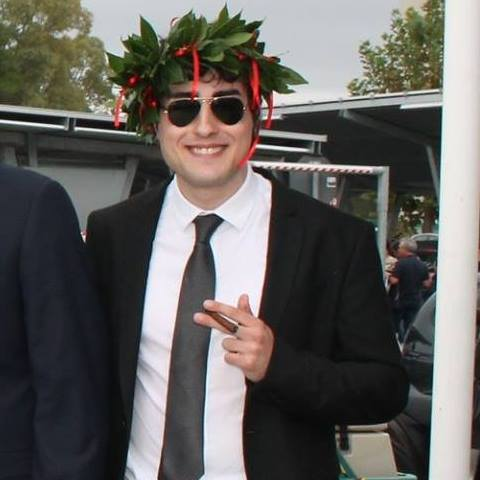
\includegraphics[width=3cm]{figures/marco.jpg}
\vspace{0.3cm}

\raisebox{-0.35ex}{
\includegraphics[width=4ex]{figures/link.png}}%
\hspace{0.05cm} /marcochiarelli

\end{figure}



%BIBLIOGRAFIA - redatta con il relativo ambiente
\begin{thebibliography}{100}
\bibitem{rif1} J. Kurose, K.W. Ross, \emph{Computer Networking. A Top-Down Approach,  sixth edition}
\bibitem{rif2} B.A. Forouzan \emph{Data Communication and Networking, fifth edition}
\bibitem{rif3} P. Oppenheimer \emph{Top Down Networking Design, third edition}
\end{thebibliography}
\end{document}



%************************************************
% Chapter 2: TEORIA DELLE CODE
%************************************************
% !TEX encoding = UTF-8
% !TEX TS-program = pdflatex
% !TEX root = ../nt.tex
% !TEX spellcheck = it-IT

%************************************************
\chapter{TEORIA DELLE CODE}
\label{cap:qtheory}
%************************************************\\

\section{PROCESSI STOCASTICI}

Modello matematico di tipo probabilistico utilizzato per andare a descrivere dei fenomeni casuali che possono essere rappresentati come funzioni di un parametro che solitamente è il tempo. $\{X(t),\ t \in T\}$. Famiglia di variabili casuali $X(t)$, indicizzate dal parametro temporale $t \in T$. Potrebbe anche essere qualche altra grandezza. Le v.a. sono definite su un unico spazio campione e che assumono valori in un certo insieme $S$. I valori assunti sono detti stati. $S$ = spazio degli stati del processo. Un processo stocastico è un insieme di funzioni del tempo. $X(t)$ generica variabile casuale. $X(t)\ \in S$. Insieme di funzioni del tempo che vengono chiamate \textbf{Realizzazioni}. Spazio campione: possibili risultati.

$X(t): T \mapsto S$ SAMPLE PATHS: realizzazioni. La cosa importante è che $X(t)$ è completamente specificato in termini probabilistici se posso scrivere la CDF congiunta (e la PDF). $X(t)$ famiglia di variabili casuali. Differenti realizzazioni. Un processo stocastico è completamente specificato con la CDF congiunta per un qualsiasi insieme (sottoinsieme) di v.a. estratte dal processo. Immaginiamo di estrarre $n$ variabili casuali:

$X(t_i),\ i=1,2,\dots,n$: estrazione di $n$ variabili casuali. Per queste devo essere in grado di scrivere la CDF congiunta:

\[
	F_{\mathbf{\underline{X}}}(\underline{x}; t) := \Pr\{X(t_1) \leq x_1,\ X(t_2) \leq x_2,\ \dots,\ X(t_n) \leq x_n\}
\]

Tale è la CDF CONGIUNTA. Ricordiamo che data una variabile casuale $\xi$, abbiamo che: $F_{\xi}(t) := \Pr\{\xi\leq t\}$. 
Qui bisogna riuscire la scrivere la CDF congiunta per queste $n$ variabili casuali estratte dal processo. In alternativa, potrei considerare la PDF congiunta, la quale è la derivata della CDF. Scriviamo la \textit{ROW VECTOR NOTATION}, generalizzando le casistiche dimensionali:

\[
	\left\{
	\begin{aligned}
	&\mathbf{\underline{X}} = (X(t_1),\ X(t_2),\ \dots,\ X(t_n)) \in\R^{n\times 1}  \\
	&\underline{x} = (x_1,\ x_2,\ \dots,\ x_n) \in\R^{n\times 1}\\
	&\underline{t} = (t_1,\ t_2,\ \dots,\ t_n) \in\R^{n\times 1}
	\end{aligned}
	\right.
\]

Ricordiamo, ancora: $[f_{\mathbf{\underline{X}}}(\underline{x}; t) = \frac{\partial{F_{\mathbf{\underline{X}}}(\underline{x}; t)}}{\partial{\underline{x}}}]$.

\subsection{CATENE DI MARKOV}

Pensiamo allo spazio degli stati $S$. Questo spazio può essere continuo o discreto. Una CATENA è un processo stocastico a stato discreto. Noi tratteremo le \textit{\textbf{CATENE DI MARKOV}}. $t$ può essere continuo o discreto. Tempo continuo o tempo discreto, rispettivamente. Quando il tempo è discreto, si parla di \textit{SEQUENZA STOCASTICA}. Eventualmente potremmo avere: $X_n,\ n=0,1,2,\dots$ ovvero diverse componenti del sistema.

Noi studieremo le CATENE DI MARKOV a tempo continuo, dette \underline{CMTC}. Categoria di processi stocastici. Per questi processi di MARKOV la relazione che intercorre tra le v.a. è molto semplice. Caratterizzazione molto semplice. Questi processi soddisfano la cosiddetta:

\begin{defn}{\textbf{PROPRIET\`A DI MARKOV}}

\[
	\Pr\{X(t) \leq x\ |\ X(t_n) = x_n,\ X(t_{n-1}) = x_{n-1},\ \dots,\ X(t_0) = x_0\} = \Pr\{X(t) \leq x\ |\ X(t_n) = x_n\}
\]

con $t > t_n > t_{n-1} >\ \dots\ > t_0$. 
\end{defn}

Questo è un processo stocastico $\{X(t),\ t\in T\}$ che soddisfa alla proprietà di MARKOV. Si tratta di una CDF condizionata. Cosa mi dice? L'evoluzione futura del processo a partire dall'istante $t_n$ non dipende dalla storia passata ma solo dallo stato finale del processo! L'evoluzione del processo da $t_n$ in poi dipende soltanto da $t_n$. Lo stato in $t_n$ riassume tutta la storia passata del processo. $\{X(t),\ t\in T\}$. Noi studieremo le catene di Markov a tempo continuo (stato discreto, tempo continuo). 

\begin{defn}{\textbf{CM omogenea}}

Invariante rispetto a traslazioni temporali degli assi:

\[
	\Pr\{X(t) \leq x\ |\ x(t_n) = x_n\} = \Pr\{X(t-t_n) \leq x\ |\ X(0) = x_n\}
\]

con $t > t_n$.
\end{defn}

Sono sostanzialmente delle catene per modellare sistemi il quale comportamento NON dipende dal tempo di osservazione. Scelta possibile dell'arco temporale. \underline{OMOGENEIT\`A}.

\begin{defn}{\textbf{COIMPLICAZIONE DELLA PROPRIET\`A DI MARKOV (\textit{tempo di soggiorno})}}

$W_i,\ i\in S$. Uno stato i qualsiasi della mia catena dev'essere una v.a. priva di memoria. Quando una v.a. casuale soddisfa alla proprietà di assenza di memoria, vale il seguente:

\[
	[\Pr\{W_i > t+\tau\ |\ W_i > t\} = \Pr\{W_i > \tau\}]
\]

Tale è la \textit{MEMORYLESS PROPERTY}.
\end{defn}

Se l'evoluzione futura del processo a partire da $t_n$ non dipende dallo stato passato del processo, non dipenderà neanche dal tempo in cui ci è stato. L'unica distribuzione di v.a. continua che soddisfa alla proprietà di assenza di memoria è la

\begin{defn}{\textbf{ESPONENZIALE NEGATIVA UNILATERA}}

\[
	\left\{
	\begin{aligned}
	&[\underline{f_{W_i}(\tau) = a\e^{-a\tau},\ \tau \geq 0}]\\
	&\left\{
	\begin{aligned}
	&F_{W_i}(\tau) = \Pr\{W_i\leq\tau\} = 1-\e^{-a\tau},\ \tau\geq 0\\
	&F_{W_i}^c(\tau) = \Pr\{W_i\geq\tau\} = \e^{-a\tau},\ \tau\geq 0
	\end{aligned}
	\right.
	\end{aligned}
	\right.
\]

\end{defn}

Unica distribuzione di probabilità che soddisfa l'assenza di memoria. Vedremo in seguito come $a := -q_{ii}$ (velocità totale di uscita dallo stato i). Velocità o equivalentemente tasso di transizione.

Proprietà di assenza di memoria per una v.a. casuale (in particolare comporta conseguenze sul tempo di soggiorno in uno stato $i$ di una CMTC):

\[
	\Pr\{W_i > t+\tau\ |\ W_i > t\} = \Pr\{W_i > \tau\}
\]	
	
Parliamone in generale.

\begin{thrm}
L'unica PDF di una v.a. continua che soddisfa alla proprietà di ASSENZA di MEMORIA è l'ESPONENZIALE NEGATIVA UNILATERA (UEN). 
\end{thrm}

\begin{proof}{\textbf{UEN MEMORYLESS PROPERTY}}
\[
	\Pr\{W_i > t+\tau\ |\ W_i > t\} = \frac{\Pr\{W_i > t+\tau,\ W_i > t\}}{\Pr\{W_i > t\}} =(\dots)
\]

Dobbiamo dimostrare questa proprietà per la UEN: $W_i>t+\tau\supseteq W_i>t \implies$

\[ 	
	(\dots) = \frac{\Pr\{W_i > t+\tau\}}{\Pr\{W_i > t\}} = \frac{\e^{-a(t+\tau)}}{\e^{-at}} = \frac{\e^{-at}\e^{-a\tau}}{\e^{-at}} = \e^{-a\tau} = \underline{\Pr\{W_i > \tau\}}
\]

La parte sottolineata sarebbe quindi la CDF complementare $F_{W_i}^c(\tau)$ della UEN.
\end{proof}

A cosa è uguale il parametro $a$? \`E uguale ad $a = -q_{ii}$, che sarebbe la velocità (totale) di uscita dallo stato $i$, ovvero la velocità totale alla quale il processo cerca di uscire dallo stato $i$. Si scrive, posto $a := -q_{ii}$:

\[
	W_i \sim EXP(-q_{ii}),\ \forall i\in S
\]

Quindi il sistema precedente diventa:

\[
	\left\{
	\begin{aligned}
	&[f_{W_i}(\tau) = -q_{ii}\e^{q_{ii}\tau},\ \tau \geq 0]\\
	&\left\{
	\begin{aligned}
	&F_{W_i}(\tau) = \Pr\{W_i\leq\tau\} = 1-\e^{q_{ii}\tau},\ \tau\geq 0\\
	&F_{W_i}^c(\tau) = \Pr\{W_I\geq\tau\} = \e^{q_{ii}\tau},\ \tau\geq 0
	\end{aligned}
	\right.
	\end{aligned}
	\right.
\]

La proprietà di assenza di memoria per $W_i$ dice che, supponendo che il processo stia soggiornando sullo stato i da $t$ unità di tempo, la probabilità che il processo mi soggiorni ancora per altre $\tau$ unità di tempo è pari alla probabilità che il processo soggiorni per $\tau$ unità di tempo. Posto $\tau$ = RESIDUO, definiamo $\Phi_{i,t}$ come tempo di soggiorno residuo nello stato i da $t$ unità di tempo, ovvero il processo si trova già da $t$ unità di tempo nello stato i! Quindi riscriviamo la MLP.

\begin{corl}

\[
	\Pr\{\Phi_{i,t} > \tau\} = \Pr\{W_i > \tau\}
\]

La distribuzione del tempo di soggiorno residuo in un tempo $t$ (LHS) è pari alla distribuzione del tempo di soggiorno (RHS). 

\[
	\left\{
	\begin{aligned}
	&[(W_i \sim \Phi_{i,t}) \sim EXP(-q_{ii})]\\
	&f_{\Phi_{i,t}}(\tau) = -q_{ii}\e^{q_{ii}\tau},\ \tau\geq 0
	\end{aligned}
	\right.
\]

\end{corl}

Nel tempo discreto la distribuzione che soddisfa la MLP è solo quella geometrica. Noi invece lavoriamo a tempo continuo. MARKOVIANIT\`A: assenza di memoria nel processo markoviano. Tempo di soggiorno residuo e tempo di soggiorno non solo hanno la stessa medesima distribuzione esponenziale (UEN), ma sono distribuite anche con lo stesso parametro $-q_{ii} = a$!

Riscriviamo la proprietà di Markov a tempo continuo! (specializzazione): Stiamo lavorando con \underline{CMTC} o CTMC (Continuos Time Markov Chain):

\[
	\Pr\{X(t_{n+1}) = x_{t_{n+1}}\ |\ X(t_n) = x_n,\ X(t_{n-1}) = x_{n-1},\ X(t_0) = x_0\} =
\]
\[
	= \Pr\{X(t_{n+1}) = x_{t_{n+1}}\ |\ X(t_n) = x_n\}
\]

$\forall x_k \in S,\ t_{n+1} > t_n > t_{n-1} >\ \dots\ > t_0$.

Chiamiamo il secondo membro \underline{probabilità di transizione}: $[\Pr\{X(t_{n+1}) = x_{n+1}\ |\ X(t_n) = x_n\}]$. Supponendo che nel tempo $t_n$ il processo si trovi in $x_n$, essa è la probabilità che al tempo $t_{n+1}$ si trovi allo stato $x_{n+1}$. Ma essa non fornisce informazioni circa quello che potrebbe accadere nel frattempo tra $t_n$ e $t_{n+1}$!

\begin{defn}{\textbf{Probabilità di Transizione da i a j}}
\[
	[\underline{p_{ij}(t,\theta) := \Pr\{X(\theta) = j\ |\ X(t) = i\}}]
\]
\end{defn}

$\forall i,j\in S$, e supponendo naturalmente che $\theta > t$.

Se la CMTC è OMOGENEA, queste probabilità di transizione non dipendono dagli istanti di tempo, ma dalla differenza dei due istanti di tempo $[\tau := \theta-t]$.

\[
	[p_{ij}(t,\theta) := \underline{P_{ij}(\tau)} = \Pr\{X(t+\tau) = j\ |\ \underline{\underline{X(t) = i}}\}]
\]

Supponendo che all'istante di tempo $t$ lo stato sia i, quella è la probabilità che dopo $\tau$ istanti di tempo lo stato sia j. Non ci riferiamo più necessariamente ai singoli istanti di tempo. Vale: $[\sum_{j\in S}{p_{ij}(\tau)} = 1]$. Distribuzione al tempo $t$: intendiamo l'insieme di queste probabilità:

\begin{defn}{\textbf{Distribuzione al tempo t}}

\[
	\pi_i(t) := \Pr\{X(t) = i\}\ \forall i\in S
\]
\end{defn}

Andiamo a considerare tutti gli stati del mio processo. Per il teorema delle probabilità totali questa probabilità la posso scrivere in tal modo:

\[
	\pi_i(t) := \Pr\{X(t) = i\} = \sum_{j\in S}{\Pr\{X(t) = i\ |\ X(0) = j\}\Pr\{X(0) = j\}} = \sum_{j\in S}{\underline{p_{ji}(t)}\underline{\pi_j(0)}}
\]

Quindi questa distribuzione al tempo $t$ la possiamo ottenere come somma di prodotti tra la distribuzione iniziale e la probabilità di transizione da j ad i. Possiamo inoltre, dato $\pi_j(0)$, conoscere qualsiasi CDF congiunta. Per ogni processo particolare posso scriverle facilmente... A tempo continuo le probabilità di transizione dipendono però dal tempo! $(\dots) = \mathord{\cdot}(t)$! Per semplificare la vita, sono state introdotte delle quantità legate a $\underline{p_{ji}(t)}$, generalmente anch'esse dipendenti dal tempo, ma che, nel caso in cui la CMTC sia OMOGENEA, sono invece costanti. Queste quantità sono quindi costanti e sono chiamate TASSI o \textit{VELOCIT\`A DI TRANSIZIONE}. Ciò che NON è costante è invece la probabilità di transizione.

\subsubsection{Tassi di Transizione}

\begin{defn}{\textbf{TASSI (o VELOCIT\`A) di transizione}}

Relazione che lega i tassi di transizione alle probabilità di transizione.
Se la catena è regolare:

\[
	\left\{
	\begin{aligned}
	&\exists q_{ij} := \lim_{\Delta t\to 0}{\frac{p_{ij}(\Delta t)}{\Delta t}},	\forall (i\neq j)\in S\\
	&\exists q_{ii} := \lim_{\Delta t\to 0}{\frac{p_{ii}(\Delta t)-1}{\Delta t}} \leq 0
	\end{aligned}
	\right.
\]

$\forall i,j\ \in S$.
\end{defn}

Si può dimostrare che questi limiti, queste quantità, esistono se la CMTC è REGOLARE, ovvero se:

\begin{defn}{\textbf{CMTC REGOLARE}}

\[
	\forall X(0),\ [\underline{\cardinality{transizioni(\Delta t < +\infty)} < +\infty}]
\]
\end{defn}

Questo deve valere per qualunque stato iniziale. $-q_{ii} \geq 0$. Supponiamo che lo stato del processo in $t$ sia $i$ $\iff X(t) = i$. La probabilità che in un intervallo $\Delta t$ tendente a 0 ($\iff \Delta t \to 0$) vi sia una transizione al di fuori di i è: $[-q_{ii}\Delta  t + o(\Delta t)]$.
Ragioniamo invece su $p_{ii}(\Delta t)$: essa rappresenta la probabilità che lo stato presente sia $i$ e tra $\Delta t$ unità di tempo lo stato sia di nuovo $i$. Tale probabilità non mi dice nulla su tutte le possibili transizioni che ci possono essere tra $t$ e $t+\Delta t$.

$1-p_{ii}(\Delta t),\ \Delta t \to 0$ è la probabilità che dopo $\Delta t$ unità di tempo lo stato NON sia più $i$, partendo da $i$ (prob. che vi sia una transizione). Quando $\Delta t \to 0$, questa probabilità tende alla probabilità di leaving dallo stato $i$. Quindi invertendo la seconda equazione del precedente sistema troviamo che al limite essa è uguale a: $[-q_{ii}\Delta t + o(\Delta t)]$. La probabilità è tanto più grande quando $q_{ii}$ è alto in modulo! Più velocemente esce, più è probabile che esca! Più grande è il valore $\abs{q_{ii}}$, più il processo cerca di uscire velocemente, e quindi con maggior probabilità vi riuscirà $\implies \abs{q_{ii}} \uparrow \implies$ processo più velocemente tende ad uscire.

$-q_{ii}$ è quindi la velocità alla quale un processo lascia lo stato $i$. In sostanza, $-q_{ii}$ rappresenta il numero medio di transizioni al di fuori di $i$ $\forall$ unità di tempo \newline
\underline{in cui il processo si trova nello stato $i$}.

Prendiamo per esempio due diverse realizzazioni dello stesso processo: $\{X^{(1)}(t),\ X^{(2)}(t)\}$. Per $X^{(1)}(t)$ abbiamo diversi soggiorni nello stato i. Supponiamo che la somma delle durate di soggiorno in $i$ facciano $1s$. Durante questa unità di tempo in cui il processo si trova in $i$, si trovano 7 transizioni al di fuori di $i$. Per $X^{(2)}(t)$, supponiamo lo stesso caso ma con 5 transizioni. Abbiamo detto che: $-q_{ii}$ è il numero medio di transizioni al di fuori dello stato $i$. Una transizione uscente segue un \underline{tempo di soggiorno}. $-q_{ii}$ rappresenta quindi anche il tempo medio di soggiorno. Ricordando che $f_{W_i}(\tau) = -q_{ii}\e^{q_{ii}\tau}$, abbiamo che:

\[
	\E[W_i] = \frac{1}{-q_{ii}}
\]

Se calcoliamo il valor medio (la media) di $f_{W_i}(\tau)$, esce proprio $(\frac{1}{-q_{ii}})$; tanto più grande è $q_{ii}$, tanto basso sarà il tempo di soggiorno in media.

Significato di $q_{ij}$. Supponiamo che attualmente il processo si trovi in $i$. La probabilità che in un intervallo di tempo infinitesimo ($\Delta t \to 0$) vi sia una transizione $ij$, ($i \rightarrow j$), è uguale alla probabilità $q_{ij}\Delta t + o(\Delta t)$. Consideriamo $p_{ij}(t)$. Non mi dice nulla, essendo una probabilità di transizione, su cosa sia eventualmente accaduto nel rispettivo intervallo di tempo tra la transizione.

Accade quindi che:

\[
	[\lim_{\Delta t \to 0}{\frac{p_{ij}(t)}{\Delta t}} = q_{ij}]
\]

(probabilità tanto più grande quanto più grande è $q_{ij}$).
La velocità è $q_{ij}$. Rappresenta una velocità alla quale si verifica la transizione $i \rightarrow j$. Ecco perché viene detto TASSO (o VELOCIT\`A) di TRANSIZIONE da $i$ a $j$. Ma è anche in sostanza il numero medio di transizioni da $i$ a $j$ $(i \rightarrow j) \ \forall$ unità di tempo in cui il processo si trova nello stato i$i$ Ragioniamo di nuovo sulle due funzioni rappresentanti due diverse realizzazioni dello stesso processo. Supponiamo sempre che la durata complessiva di un soggiorno in $i$ sommi temporalmente ad 1. $q_{ij}$ si differenzia da $-q_{ii}$ in quanto rappresenta il numero medio di transizioni ($i \rightarrow j$).

\[
	\sum_{(j\neq i)\in S}{q_{ij}} = \sum_{(j\neq i)\in S}{(\lim_{\Delta t \to 0}{\frac{p_{ij}(\Delta t)}{\Delta t}})} = \lim_{\Delta t \to 0}{\sum_{(j\neq i)\in S}{(\frac{p_{ij}(\Delta t)}{\Delta t})}} = (\dots)
\]

Considerando uno stato $i$ qualsiasi, questa sommatoria fa 1: $\iff \sum_{j\in S}{p_{ij}(\Delta t)} = 1$. Quindi:

\[
	(\dots) = \lim_{\Delta t \to 0}{\frac{1-p_{ii}(\Delta t)}{\Delta t}} = \underline{\underline{-q_{ii}}}
\]

La quale è la velocità \underline{totale} di uscita dallo stato $i$. Introduciamo ora una seconda quantità: $[\tau_{i,j} = \frac{q_{ij}}{-q_{ii}}]$, ovvero la probabilità che il processo, lasciando lo stato i, faccia una transizione verso lo stato $j$. 

Supponiamo che $q_{ij}=10,\ q_{ik}=30,\ q_{ih}=60$... mediamente vi siano quindi 100 transizioni uscenti. $-q_{ii} = \sum_{(j\neq i)\in S}{q_{ij}} = 100$. Abbiamo che:

\[
	\left\{
	\begin{aligned}
	&\tau_{i,j} = \frac{10}{100} = 0.1\\
	&\tau_{i,h} = \frac{60}{100} = 0.6\\
	&\tau_{i,k} = \frac{30}{100} = 0.3
	\end{aligned}
	\right.
\] 

$\tau_{i,j}$ è quindi alla fine la probabilità che, supponendo di lasciare $i$, la transizione sia verso $j$. LASCIANDO LO STATO $i$, $\exists$ UNA TRANSIZIONE VERSO LO STATO $j$.

Distribuzione al tempo $t$. Ci sono dei sistemi di equazioni differenziali che legano la distribuzione al tempo $t$ ai tassi di transizione:

\[	
	\left\{
	\begin{aligned}
	&\underline{\pi_i}(t) := \Pr\{X(t) = i\},\ \forall i\in S\\
	&\frac{d \pi_i(t)}{dt} = \sum_{j\in S}{q_{ji}\pi_j(t)},\ \forall i\in S
	\end{aligned}
	\right.
\]

Di queste equazioni differenziali ve n'è una $\forall s\in S$ della nostra catena. Nella maggior parte dei casi, non ci serve $\pi_i(t)$, ma una distribuzione a regime (costante). A regime serve la rispettiva distribuzione a regime (dopo un tempo molto grande). Ci sono delle condizioni in base alla quale $\pi_i(t) \to K \neq \mathord{\cdot}(t)$ (distribuzione di equilibrio, a regime). Ma quali sono queste condizioni?

\subsection{Probabilità a regime}

Quali sono le condizioni di esistenza delle probabilità di stato a regime? Introduciamo alcune definizioni. Consideriamo uno stato $i \in S$ della mia \underline{CMTC}. Diciamo che lo stato $(i\in S)$ è \textit{TRANSITORIO} se c'è una probabilità non nulla che il processo non torni più in quello stato dopo che esso viene lasciato. Si dirà \textit{RICORRENTE} in caso contrario (se con probabilità 1 torni nello stato $i$ dopo averlo lasciato). Ai fini della distribuzione di regime, a noi interessano i RICORRENTI (gli stati ricorrenti). Sia $M_i$ il tempo medio di ritorno (o \underline{di ricorrenza} nello stato $i$). Per tempo di ritorno si intende il tempo che passa da \underline{due ingressi consecutivi} nello stato $i$. $M_i$ dice quanto dura in media questo tempo (ovviamente guardando tutte le possibili realizzazioni, altrimenti sarebbe costante). Si consideri una finestra temporale ($M_i$), è contemplato in media un solo soggiorno in $i$! (UN SOLO tempo di soggiorno). Se questo valore diverge ($\iff M_i \to +\infty$), lo stato è detto \textit{RICORRENTE NULLO}. Se $M_i$ converge parliamo di STATO \textit{RICORRENTE NON NULLO}.

Consideriamo ora un sottoinsieme proprio dello spazio degli stati $A\subset S\ |\ \bar{A} \cup A = S$. $A$ comprende una parte degli stati, e non può coincidere con $S \iff \bar{A} = S \setminus (A\neq \emptyset)$.

Vale:

\begin{thrm}
$A$ chiuso se:

\[
	\sum_{i\in A}{\sum_{j\in\bar{A}}{q_{ij}}} = 0
\]
\end{thrm}

Significa che una volta che il processo entra in $A$, NON esce da $A$! In particolare, chiamiamo \textit{STATO TRAPPOLA} od \textit{ASSORBENTE} uno stato $i$ per il quale: $ [q_{ii} = -q_{ii} = 0]$ (Il processo NON esce più da quello stato). Uno STATO TRAPPOLA corrisponde ad un insieme chiuso costituito da solo quello stato.

\begin{defn}{\textbf{CM IRRIDUCIBILE}}

Una CTMC è \underline{\underline{IRRIDUCIBILE}} se $\nexists$ insiemi chiusi $\iff$ Tutti gli stati COMUNICANO tra di loro. Da $i$ a $j$ ci arrivo (magari passando da altri stati), ma ci arrivo sempre prima o poi! $i \leftarrow\rightarrow j\ \forall i,j\in S$.

\end{defn}

Abbiamo quindi tre caratterizzazioni di stato: (tre diversi possibili tipi di stato):

\begin{itemize}

\item{\textit{TRANSITORI}};
\item{\textit{RICORRENTI NULLI}};
\item{\textit{RICORRENTI NON NULLI}}.

\end{itemize}

\begin{corl}{\textbf{Omogeneità dei tipi di stato per CM IRRIDUCIBILE}}

Qualora una CM sia IRRIDUCIBILE $\implies$ allora tutti gli stati sono dello stesso tipo.

\end{corl}

Concetto molto forte. CATENA IRRIDUCIBILE $\iff$ tutti gli stati comunicano $\iff$ tutti gli stati sono dello stesso tipo. Ricordiamo:

\[
	[\frac{d \pi_i(t)}{dt} = \sum_{j\in S}{q_{ji}\pi_j(t)}]
\]

\begin{defn}{\textbf{PROBABILIT\`A LIMITE}}
\[
	[\pi_i := \lim_{t\to\infty}{\pi_i(t)}]
\]
$\forall i\in S$.
\end{defn}

Se una CATENA è OMOGENEA, IRRIDUCIBILE (Quando una CATENA è OMOGENEA i tassi di transizione sono COSTANTI), allora:

\[
	\exists \lim_{t\to\infty}{\pi_i(t)} := \pi_i \neq \mathord{\cdot} \pi_i(0)
\]

Se vogliamo avere delle distribuzioni a regime, vogliamo che questa quantità esista finita (limite esistente e convergente). In particolare non devono dipendere dalle probabilità di \underline{stato iniziali}. In tal caso il sistema di equazioni differenziali collassa in un sistema di equazioni algebriche lineari:

\[
	[\sum_{j\in S}{q_{ji}\pi_j} = 0]
\]

$\forall i\in S$. Le derivate vanno quindi a 0 $\iff \pi_i(t) \tendsto{t\to\infty} \pi_i$. Questo sistema è OMOGENEO (sicuramente comprende la soluzione nulla). Tante soluzioni quanti sono gli stati del processo. SE la soluzione nulla fosse l'unica soluzione, gli stati saranno tutti TRANSITORI o tutti RICORRENTI nulli e non avremmo quindi una distribuzione di regime ($\iff \nexists \pi_i$). Se così non fosse invece, in tal caso le soluzioni saranno un numero infinito, che differirranno per una \underline{costante moltiplicativa} tra di loro. Se sono infinite (tutte linearmente dipendenti), tra tutte queste le filtriamo con la cosiddetta condizione di normalizzazione. In tal caso gli stati saranno tutti \underline{RICORRENTI NON NULLI}.

\begin{defn}{\textbf{ERGODICIT\`A}}

\[
	\left\{
	\begin{aligned}
	&\sum_{j\in S}{q_{ji}\pi_j} = 0,\ \forall i\in S\\
	&\sum_{i\in S}{\pi_i} = 1
	\end{aligned}
	\right.
\]

$\exists SOL$? Se esiste, in tal caso la CATENA è detta \textit{ERGODICA} (proprietà di ERGODICIT\`A). \underline{CMTC} \{OMOGENEA, IRRIDUCIBILE, (STATI RICORRENTI NON NULLI)\}.\end{defn}

Innanzitutto, si verifichi l'OMOGENEIT\`A guardando i tassi di transizione (diagrammi di stato). Devono essere costanti (OMOGENEA, \underline{\underline{IRRIDUCIBILE}} (stati dello stesso tipo)). Basterebbe, per verificare che gli stati siano TUTTI ricorrenti non nulli, verificare questa proprietà per UN SOLO STATO! Ma a questo punto, senza ragionare su $M_i$, ragiono sull'equazione e la risolvo, sperando di risolverla e di trovare UNA ed UNA SOLA soluzione.

\begin{corl}{\textbf{Caratterizzazione dell'Ergodicita'}}

Se abbiamo una [CMTC OMOGENEA, IRRIDUCIBILE e con un numero di stati finito $(\iff\cardinality{stati}<+\infty)$], sicuramente essa è \underline{ERGODICA}].

\end{corl}

Abbiamo detto che $\pi_i,\ i\in S$ sono le probabilità limite, QUANTIT\`A valutate IN VERTICALE, ed hanno a che fare con le distribuzioni di regime. MA è anche la frazione di tempo a regime in cui lo stato sia $i$.

\subsection{ERGODICIT\`A}

Condizioni di ERGODICIT\`A per una CMTC: \{OMOGENEA, IRRIDUCIBILE, con STATI RICORRENTI NON NULLI\} $\implies [\exists \lim_{t\to\infty}{\pi_i(t)} := \pi_i]$. Una volta veriifcate queste due proprietà, non c'è bisogno di verificare che gli stati siano tutti RICORRENTI NON NULLI. In maniera più semplice si tenta di risolvere quel sistema sperando che abbia una soluzione non banale. Diagramma dei tassi di transizione: \{Cerchi = Stati, Archi = Transizioni, pesate con i tassi di transizione\}. Se questi tassi non sono dipendenti dal tempo allora la catena è OMOGENEA. 

\[
	[\underline{\pi_i} = \lim_{t\to\infty}{(\pi_i(t) = \Pr\{X(t)=i\})},\ \forall i\in S
\]

La distribuzione di regime ha ovviamente a che fare con le probabilità limite. Immaginiamo che la catena sia ERGODICA. $\pi_i$ = probabilità che a regime lo stato sia $i$. Se la catena è \underline{ergodica}, allora a $\pi_i$ possiamo attribuire un altro significato: frazione del tempo (A REGIME) in cui lo stato sia $i$:

\[
	[\pi_i = \lim_{t\to\infty}{\frac{T_i(t)}{t}}]
\]

dove $T_i(t)$ è il tempo trascorso dal processo \underline{nello stato $i$} sino al tempo $t$. (SINGOLA REALIZZAZIONE). \`E come se stessimo guardando una singola realizzazione del processo. Presa una finestra $[0,t) \leftarrow T_i(t)$. Fino al tempo $t$. Se calcolo $\frac{T_i(t)}{t}$, allora ottengo la frazione di tempo nel quale il processo è stato nello stato $i$ nell'intervallo di tempo definito dalla finestra temporale scelta.

es. $\pi_i = 0.2 \implies$ per il 20\% il processo a regime si è trovato in $i$. $\pi_i\tau$ rappresenta il tempo in media nel quale il processo si è trovato nello stato $i$ durante la finestra temporale di durata $\tau$. $\pi_i$ è da valutare sull'INSIEME delle realizzazioni.

Consideriamo $N(t)$ processo stocastico che rappresenta il numero di clienti (\#) in un sistema a coda. Esaminiamo un certo numero di realizzazioni.

Dal momento che $\pi_i(t)$ è una probabilità, essa va valutata in verticale. Supponiamo che:

\[
	\left\{
	\begin{aligned}
	&n_R := \cardinality{realizzazioni\ di\ N(t)}\\
	&n_i(t) := n_i = \cardinality{realizzazioni\ con\ stato\ i\ nell'istante\ t}
	\end{aligned}
	\right.
\]

$(\frac{n_i}{n_R})$ rappresenta la frazione delle $n_R$ realizzazioni con stato pari ad $i$ in $t$. Quando $n_R$ cresce, $\iff n_R \uparrow ,\ (\frac{n_i}{n_R}) \tendsto{}$ probabilità che lo stato del processo sia $i$.

Rispettivamente:

\begin{thrm}{\textbf{Probabilità Limite}}

\[
	\lim_{n_R\to\infty}{(\frac{n_i}{n_R})} = \pi_i(t) = \Pr\{X(t)=i\}
\]
\end{thrm}

Tutto questo a regime! Abbiamo considerato $\pi_i$ valutandola con un numero molto grande di realizzazioni. Guardando invece ad una singola realizzazione di tempo molto grande ($\iff t\to +\infty$), abbiamo che: $\underline{\pi_i} = \lim_{t\to\infty}{\frac{T_i(t)}{t}}$, che sarebbe la frazione in cui il processo si è trovato in $i$ nella finestra temporale $[0,t)$.

\begin{thrm}{\textbf{Mapping VERTICALE ORIZZONTALE}}

Se c'è l'ERGODICIT\`A abbiamo che:

\[
	\underline{\pi_i} = \lim_{n_R\to\infty}{(\frac{n_i}{n_R})} = \pi_i(t) = \Pr\{X(t)=i\} = \lim_{t\to\infty}{\frac{T_i(t)}{t}}
\]
\end{thrm}

Si consideri ora: $\bar{N} = \sum_{i=0}^\infty{i\pi_i}$. Questo è la media del numero di clienti. Numero medio di clienti del sistema a regime (si noti l'estremo superiore della sommatoria). Ma se il processo è ERGODICO, la media di insieme coincide con la media temporale. Nella pratica si suppone l'\underline{ergodicità}, si procede in orizzontale. Si consideri $\lim_{t\to\infty}{\bar{N_t}}$. Senza il limite essa rappresenta il valore medio assunto da quelle funzioni: $\bar{N_t} := \frac{1}{t}\int_0^t{N(\tau)d\tau}$ (MEDIA TEMPORALE) durante la finestra temporale $[0,t)$. Se c'è l'ERGODICIT\`A allora questa quantità, AL LIMITE di $t\to\infty$ coincide con $\bar{N} \iff [\lim_{t\to\infty}{\bar{N_t}} = \bar{N}]$ = VALORE DI REGIME.

\subsubsection{ERGODICIT\`A (RECAP)}

$\{\pi_i,\ \pi_i\tau\}$ rappresentano rispettivamente la probabilità che \underline{a regime} il processo si trovi in $i$, ed il tempo medio che il processo si trova in $i$ nella finestra temporale di lunghezza $\tau$. $M_i$ = tempo medio di ritorno nello stato $i$. Supponiamo di avere $\tau = M_i$. Sarebbe il tempo tra due ingressi consecutivi nello stato $i$ = tempo di ricorrenza. VALOR MEDIO $M_i$. \`E necessariamente un tempo di soggiorno. Quindi: 

$\pi_iM_i$ = tempo medio trascorso nello stato $i$ durante la finestra temporale $\tau = M_i$. Ma abbiamo \underline{un solo soggiorno} durante $M_i \iff [\underline{\pi_iM_i} = \E[W_i] = \frac{1}{-q_{ii}}]$. Invertendo troviamo: $M_i = \frac{1}{-q_{ii}\pi_i}$ (tempo medio di ricorrenza). Ricordiamo che:

\[
	\underline{f}_{W_i}(\tau) = -q_{ii}\e^{q_{ii}\tau},\ \tau\geq 0
\]

Ed avendo un solo soggiorno $\underline{\pi_iM_i}$ rappresenta il TEMPO \underline{MEDIO DI SOGGIORNO}. Possiamo dare una formulazione matriciale dell'insieme di equazioni differenziali:

\[
	\left\{
	\begin{aligned}
	&\frac{d \pi_i(t)}{dt} = \sum_{j\in S}{q_{ji}\pi_j(t)},\ \forall i\in S\\
	&\frac{d \underline{\pi(t)}}{dt} = \underline{\pi(t)}\underline{Q}
	\end{aligned}
	\right.
\]

$\underline{\pi}$ è il vettore riga delle probabilità di stato al tempo t, indicizzato da $i$. Nel caso di ERGODICIT\`A ovviamente vale che: $[\underline{\pi}\underline{Q} = \underline{0}]$ (vettore nullo).

\subsection{CMTC Nascita e Morte}

Caso particolare di CMTC, utili per lo studio dei sistemi a coda. CATENE DI NASCITA E MORTE per una CMTC. Caso particolare di CMTC. Sono dette così perché si prestano bene a modellare una evoluzione, dinamica di una popolazione (dimensione della popolazione). Abbiamo incrementi o decrementi di stato UNITARI $\iff\ \{i++,\ i--\}$. Ci interessano molto. Sono delle catene definite sullo spazio degli stati $S = \{0,1,2,\ \dots\}$. Tale spazio può essere di dimensione illimitata. Ma tipicamente lo spazio per noi sarà tale che $\cardinality{S} < +\infty$. Catene caratterizzate da fatto che vi sono incrementi/decrementi solo unitari.

Sia $N(t) = i$, quello che può accadere è che: $\{N(t) = i \to i+1\ \lor\ N(t) = i \to i-1\}$. Nel DTT (diagramma dei tassi di transizione), gli archi ricordiamo che rappresentano delle transizioni, e sono pesati dai tassi (o velocità) di transizione. DTT sarà fatta con cerchi che rappresentano gli stati, e gli archi rappresentanti le transizioni, pesati con i rispettivi tassi (o velocità).

\begin{center}
\begin{tikzpicture}[->, >=stealth', auto, semithick, node distance=1.9cm]
\tikzstyle{every state}=[fill=white,draw=black,thick,text=black,scale=1]
\node[state]    (0)                     {$0$};
\node[state]    (1)[right of=0]   {$1$};
\node[state]    (2)[right of=1]   {$2$};
\node[state] (d) [right of=2] {\ldots};
\node[state]    (im1)[right of=d]   {$i-1$};
\node[state]    (i)[right of=im1]   {$i$};
\node[state]    (ip1)[right of=i]   {$i+1$};
\node[state]    (d2)[right of=ip1]  {\ldots};
\path
(0) edge[bend left]     node{$\lambda_0$}         (1)
(1) edge[bend left]     node{$\lambda_1$}         (2)
    edge[bend left,below]    node{$\mu_1$}            (0)
(2) edge[bend left]     node{$\lambda_2$}           (d)
    edge[bend left,below]    node{$\mu_2$}             (1)
(d) edge[bend left]         node{$\lambda_{i-2}$}   (im1)
	edge[bend left,below]   node{$\mu_3$}          (2)
(im1) edge[bend left]       node{$\lambda_{i-1}$}  (i)
	  edge[bend left,below]   node{$\mu_{i-1}$}     (d)
(i)   edge[bend left]   node{$\lambda_i$}      (ip1)
      edge[bend left,below]  node{$\mu_i$}          (im1)
(ip1) edge[bend left]       node{$\lambda_{i+1}$}  (d2)
	 edge[bend left,below]   node{$\mu_{i+1}$}      (i)
(d2) edge[bend left,below]   node{$\mu_{i+2}$}     (ip1);
\end{tikzpicture}
\end{center}

Tipicamente in un DTT per una catena di questo tipo abbiamo che sopra ci sono le nascite ($\lambda_i$), e sotto vi sono le morti ($\mu_i$). Rispettivamente:

\begin{defn}{\textbf{Tassi di nascita e morte}}

\[
	\left\{
	\begin{aligned}
	&\lambda_i :=\ tasso\ di\ nascita\ sullo\ stato\ i\\
	&\mu_i :=\ tasso\ di\ morte\ nello\ stato\ i
	\end{aligned}
	\right.
\]
\end{defn}

Se questi valori sono COSTANTI $\iff$ la CATENA è OMOGENEA. Se la catena è IRRIDUCIBILE: tutti gli stati comunicano $\implies [\exists\pi_i = \lim_{t\to\infty}{\pi_i(t)}]\ \forall i\in S$. Il numero di stati però NON è finito! $(\iff \cardinality{S} = +\infty)$. Quindi dobbiamo cercare di risolvere il sistema:

\[
	\left\{
	\begin{aligned}
	&\sum_{j=0}^\infty{q_{ji}\pi_j} = 0\\
	&\sum_{i=0}^\infty{\pi_i} = 1\ (CONDIZIONE\ DI\ NORMALIZZAZIONE)
	\end{aligned}
	\right.
\]

Abbiamo che: $-q_{00} = \lambda_0$ (velocità totale di uscita dallo stato 0). Quindi: $-\lambda_0\pi_0 + \mu_1\pi_1 = 0$ per lo stato 0, poi dato che vale: $-q_{11}=\lambda_1 + \mu_1$, allora per lo stato 1: $\lambda_0\pi_0 -( \lambda_1+\mu_1)\pi_1 + \mu_2\pi_2 = 0$. Genericamente allo stato i abbiamo:

\[
	"i" \rightarrow\ \lambda_{i-1}\pi_{i-1} - (\lambda_i +\mu_i)\pi_i + \mu_{i+1}\pi_{i+1} = 0
\]

Queste si chiamano EQ. DI BILANCIAMENTO TOTALE. Noi scriviamo le equazioni in generale per una \underline{CMTC ERGODICA}. $\sum_{j\in S}{q_{ji}\pi_j} = 0\ \forall i\in S$. Proviamo a tirare fuori il termine della sommatoria per $j=i$:

\[
	\implies \sum_{(j\neq i)\in S}{q_{ji}{\pi_j}} = -q_{ii}\pi_i
\]

Generalizzando possiamo scrivere le:


\begin{thrm}{\textbf{EQUAZIONI DI BILANCIAMENTO TOTALE}}

\[
	\sum_{(j\neq i)\in S}{q_{ji}\pi_j} = \sum_{(j\neq i)\in S}{q_{ij}\pi_i}
\]

\end{thrm}

Esse esprimono il fatto che a regime (od equilibrio), la frequenza delle transizioni entranti nello stato $i$ eguaglia la frequenza delle transizioni uscenti dallo stato $i$. \`E sostanzialmente un altro modo di scrivere: $\sum_{j\in S}{q_{ji}\pi_j} = 0\ \forall i\in S$. Il numero medio (per unità di tempo) di transizioni entranti nello stato $i$ è uguale al numero medio di transizioni uscenti nello stato $i$. $q_{ji}\pi_j$ è la frequenza (quindi adimensionale) delle transizioni dallo stato $j$ allo stato $i$. Numero medio di transizioni nello stato $i$ (per unità di tempo).

$q_{ji}$ = numero medio di transizioni da $j$ ad $i\ \forall$ unità di tempo in cui il processo si trova nello stato $j$, mentre $\pi_j$ è una frazione di tempo. Ricordiamo che scelta ad esempio una finestra temporale $\tau=1s$, allora il prodotto $\pi_j\tau$ rappresenta il tempo medio trascorso durante questa finestra temporale ($\tau=1s$) dal processo nello stato $j$. Se facciamo $q_{ji}\pi_j$ otteniamo invece il numero medio di transizioni da $j$ ad $i$ $\forall$ unità di tempo. 

L'intera equazione dice che all'equilibrio la frequenza delle transizioni verso lo stato $i$ è pari alla frequenza di transizioni uscenti dallo stato $i$. All'equilibro il flusso entrante nello stato $i$ è pari al suo flusso uscente. Si eguaglia praticamente ($\forall$ stato), flusso entrante (IN) e flusso uscente (OUT). Quindi dobbiamo bilanciare il flusso caso per caso.

Consideriamo l'equazione di bilanciamento per il generico stato $i$:

\[	
	(\lambda_{i-1}\pi_{i-1} + \mu_{i+1}\pi_{i+1} = IN) = ((\lambda_i +\mu_i) = OUT)
\]

Per lo stato 0 abbiamo: $\mu_1\pi_1 = \lambda_0\pi_0$.
Vale per qualunque CMTC \underline{ERGODICA}.

\begin{thrm}{\textbf{EQUAZIONI DI BILANCIAMENTO TOTALE generalizzate}}

Possiamo considerare $(A \subset S) \supset \{statuses\}$. Si immagini di considerare come macrostati gli insiemi di stato $\{0,\ \dots,\ i\}$. Valgono le eq. di bilanciamento totale generalizzate: Flusso uscente da A = flusso entrante in A:

\[
	\sum_{j\in \bar{A},i\in A}{q_{ij}\pi_i} = \sum_{j\in \bar{A},i\in A}{q_{ji}\pi_j}
\]

\end{thrm}

Inoltre, ne deriva che per una BDCMTC abbiamo di conseguenza:

\begin{corl}{\textbf{EQUAZIONI DI BILANCIAMENTO TOTALE GEN. per BD-CMTC}}

\[
	[(\lambda_i\pi_i)_{OUT} = (\mu_{i+1}\pi_{i+1})_{IN}]
\]

\end{corl}

Tentiamo ora di eguagliare il flusso sulla frontiera verticale tra due stati. Otteniamo:

\begin{thrm}{\textbf{EQUAZIONI DI BILANCIAMENTO LOCALE}}


\[
	\pi_iq_{ij} = \pi_jq_{ji}
\]

\end{thrm}

QUESTE valgono soltanto IN CASI PARTICOLARI (BDCMTC). Le GLOBALI e quelle GLOBALI GENERALIZZATE valgono invece SEMPRE per una CMTC.

Si considerino queste equazioni trovate per una BDCMTC:

\[
	\left\{
	\begin{aligned}
	&\lambda_i\pi_i = \mu_{i+1}\pi_{i+1},\ i\geq 0\\
	&\sum_{i=0}^\infty{\pi_i} = 1\ as\ C.N.
	\end{aligned}
	\right.
\]

Quindi abbiamo: $\pi_{i+1} = \frac{\lambda_i \pi_i}{\mu_{i+1}}$. Prendiamo $(i=0) \implies \pi_1 = \pi_0 \frac{\lambda_0}{\mu_1}$. Andando avanti ricorsivamente troviamo:

\[
	\left\{ 
	\begin{aligned}
	&i=1 \implies \pi_2 = \pi_1 \frac{\lambda_1}{\mu_2} = (\pi_0 \frac{\lambda_0}{\mu_1})\frac{\lambda_1}{\mu_2}\\
&i=2 \implies \pi_3 = \pi_2 \frac{\lambda_2}{\mu_3} = (\dots) = \pi_0 \frac{\lambda_0\lambda_1\lambda_2}{\mu_1\mu_2\mu_3}\\
&i-1 \implies \underline{\pi_i} = \pi_0 \frac{\lambda_0\lambda_1\lambda_2\dots\lambda_{i-1}}{\mu_1\mu_2\dots\mu_i} = \pi_0\prod_{k=0}^{i-1}{\frac{\lambda_k}{\mu_{k+1}}},\ i \geq 1
	\end{aligned}
	\right.
\]

Abbiamo quindi trovato le espressioni per le:

\begin{defn}{\textbf{Probabilità a regime}}

\[
	[\underline{\pi_i} = \pi_j\prod_{k=j}^{i-1}{\frac{\lambda_k}{\mu_{k+1}}}] = \mathord{\cdot}(\pi_j)
\]
\end{defn}

Adesso vogliamo mettere in gioco la condizione di normalizzazione: Quindi essa diventa:

\[
	[\pi_0 + \sum_{i=1}^{\infty}{\pi_i} = 1] \implies \pi_0 + \sum_{i=1}^{\infty}{\pi_0\prod_{k=0}^{i-1}{\frac{\lambda_k}{\mu_{k+1}}}} = 1 = \pi_0(1 + \sum_{i=1}^{\infty}{\prod_{k=0}^{i-1}{(\frac{\lambda_k}{\mu_{k+1}})}}) = 1 \implies
\]
\[
	\pi_0 = \frac{1}{1 + \sum_{i=1}^{\infty}{\prod_{k=0}^{i-1}{(\frac{\lambda_k}{\mu_{k+1}})}}}
\]

with:

\[
	\pi_i = [\pi_0 \prod_{k=0}^{i-1}{\frac{\lambda_k}{\mu_{k+1}}}],\ i \geq 1
\]

\begin{corl}

Se la sommatoria a denominatore di $\pi_0$ converge, allora la soluzione esiste. Quindi:

\[
	\pi_i = [\frac{1}{1 + \sum_{i=1}^{\infty}{\prod_{k=0}^{i-1}{(\frac{\lambda_k}{\mu_{k+1}})}}}] \prod_{k=0}^{i-1}{\frac{\lambda_k}{\mu_{k+1}}},	 i \geq 1
\]
\end{corl}

\newpage

\subsection{PROCESSO DI POISSON}

\`E un caso particolare di BDCMTC nel quale i tassi di nascita sono costanti e pari a $\lambda_i = \lambda \neq \mathord{\cdot}(i)\ \land\ \mu_i = 0\ \forall i\in S$. \`E sottinteso che il processo sia omogeneo. Il processo è di pura nascita. Lo spazio degli stati è il seguente: $S = \{0,1,2,\ \dots\}$. Tutti gli stati sono TRANSITORI (una volta uscito da uno stato NON vi ritorno più) $\implies \nexists (\pi_i \neq \mathord{\cdot}(t))$. 

\[
	\left\{
	\begin{aligned}
	&\frac{d \pi_i(t)}{dt} = \sum_{j\in S}{q_{ji}\pi_j(t)},\ \forall i\in S\\
	&\underline{\underline{\pi_0(0)}} = 1
	\end{aligned}
	\right.
\]

dove l'ultima equazione del sistema rappresenta la condizione iniziale, sempre da rispettare. Per un processo di POISSON abbiamo che la distribuzione soddisfa alla seguente:

\begin{defn}{\textbf{Funzione massa di probabilità per un Processo di POSSION}}

\[
	\pi_i(t) = \Pr\{X(t) = i\} = \frac{(\lambda t)^i}{i!}\e^{-\lambda t},\ t\geq 0,\ \forall i\in S
\]

\end{defn}

Questa espressione mi ricorda la distribuzione di POISSON con parametro $(a := \lambda t)$. Avendo una v.a. distribuita con Poisson con parametro $a \implies a = \E[X]$. Disegnamo una possibile realizzazione del processo. Supposto che evolva a partire dallo stato 0. Abbiamo:

$\{\tau_1 = W_1,\ \tau_2 = W2,\ \dots,\ \tau_n = t_n-t_{n-1}\}$. Possiamo quindi scrivere la PDF del tempo di soggiorno negli stati:

\[
	[f_{\tau_n}(r) = \lambda\e^{-\lambda r},\ r \geq 0]
\]

ove (\underline{$\tau_n$ = tempo di soggiorno negli stati}). Queste variabili casuali sono distribuite secondo Poisson. Il processo di POISSON modella gli arrivi dei pacchetti alle code dei router. Arrivi dei clienti in un sistema a coda. Supponiamo di utilizzare al posto di $X(t)$, $A(t)$. \textit{ARRIVAL}. Posso dire che questo processo CONTEGGIA gli arrivi sino a $t$. PROCESSO DI CONTEGGIO DEGLI ARRIVI sino a $t$. $\tau$ sono tempi di INTER-ARRIVO (quanto tempo è passato tra l'arrivo del cliente (n-1)-esimo e quello n-esimo) $\iff [\tau_n = t_n - t_{n-1}]$ sono i tempi di inter-arrivo tra i clienti. SE STO UTILIZZANDO UN PROCESSO DI POISSON per modellare GLI ARRIVI, allora abbiamo che il tempo di soggiorno è sempre distribuito esponenzialmente in maniera negativa unilatera. 

\begin{corl}{\textbf{Omogeneità del Processo di POISSON}}

\[
	\left\{
	\begin{aligned}
	&\Pr\{A(t) = i\} = \frac{(\lambda t)^i}{i!}\e^{-\lambda t}\\
	&\Pr\{A(t)-A(s<t) = i\} = \frac{(\lambda \tau)^i}{i!}\e^{-\lambda \tau}
	\end{aligned}
	\right.
\]

con $\tau := t-s$. 

\end{corl}

Il precedente corollario vale GRAZIE AL FATTO CHE LA CATENA \`E OMOGENEA. 

\subsubsection{RECAP}

Processo di Poisson, caso particolare di una CMTC di nascita e morte (BDCMTC). Tipicamente utilizzato per modellare i clienti in ARRIVO ad un sistema a coda. In questo caso lo possiamo vedere come un processo di conteggio degli arrivi. I tempi di interarrivo sono v.a. indipendenti identicamente distribuite con distribuzione esponenziale negativa unilatera. Rispettivamente, le variabili casuali $[\tau_n = t_n-t_{n-1}]$ avranno questa PDF (tempi di interarrivo):

\[
	PDF:\ f_{\tau_n}(r) = \lambda\e^{-\lambda r},\ r \geq 0
\]

ovvero che $\tau_n \sim EXP(\lambda)$, e che quindi $\implies \E[\tau_n] = \frac{1}{\lambda}$, che sarebbe quindi il tempo medio di interarrivo tra i clienti. ANALISI MARKOVIANA. Per quanto riguarda gli arrivi dei pacchetti nel processo si dice più che altro \textit{SELF-SIMILAR} in presenza di burst. Nella realtà gli arrivi dei pacchetti non seguono ovviamente sempre il processo di Poisson. I frattali sono dietro i processi Self-Similar. Questo modello di Poisson non tiene conto solo del burstness. Se i pacchetti aumentano regolarmente, non ci sarebbe bisogno dei buffer. Gli switch ATM sono stati modellati secondo il processo di POISSON. Prevede una burstness, ma abbastanza regolare. Gli switch ATM avevano un modellato errato degli arrivi $\implies$ cattivo dimensionamento.

\begin{thrm}{\textbf{RANDOM-SPLITTING}}

Splitting su due processi può essere generalizzato per un $\cardinality{processi} > 2$. Immaginiamo di avere un processo degli arrivi di POISSON $A(t)$, con velocità $\lambda$ (velocità media di arrivo). Supponiamo di derivare due altri processi da questo: $\{A(t) \rightarrow A_1(t),\ A_2(t)\}$. Quando arriva un nuovo cliente, con probabilità $p$ sarà assegnato ad $A_1(t)$, e con probabilità quindi $(1-p)$ al processo $A_2(t)$. Le assegnazioni sono INDIPENDENTI! Si ha: $[A(t) = A_1(t) + A_2(t)]\,\ A(t) = \cardinality{arrivi\ da\ 0\ a\ t}$. Gli arrivi si conservano! $\implies A(t) = A_1(t) + A_2(t)$. Si dimostra che $\{A_1(t),\ A_2(t)\}$ sono ancora di POISSON, con parametri rispettivamente: $\{\lambda_1=\lambda p,\ \lambda_2 = \lambda (1-p)\}$. Inoltre tali processi sono indipendenti statisticamente tra di loro. Splitting casuale mi produce ancora dei processi di Poisson in virtù dell'indipendenza delle assegnazioni;
\end{thrm}

\begin{thrm}{\textbf{POOLING}}

Combinazione. Supponiamo $\{A_1(t),\ A_2(t)\}$ di POISSON indipendenti, con velocità $\lambda_1,\ \lambda_2$, e vogliamo fare il pooling (combino gli arrivi in un solo unico processo). Si dimostra che $A(t)$ è ancora di POISSON con parametri $\underline{\lambda = \lambda_1+\lambda_2} \implies \underline{\underline{A(t) = A_1(t)+A_2(t)}}$. Quindi le velocità sono dei parametri associati ai processi del quale stiamo facendo la combinazione. Se ne considero $n$ il discorso non cambia. Perfettamente generalizzabile.
\end{thrm}

\subsection{RITARDO NELLE RETI DI DATI}

Uno degli indici di prestazioni più importante è il ritardo medio (\textit{mean delay}). Ritardo medio affinché dei dati fluiscano dall'host a destinazione. Per le applicazioni multimediali non è importante solo il ritardo medio in sé, ma proprio la sua distribuzione (CDF). Probabilità che il ritardo end-to-end sia inferiore a $100ms$ es. Teoria delle code ci fornisce degli strumenti tecnici molto importanti. Dovremo però effettuare delle ipotesi semplificative, ovvero creare un modello. Se gli arrivi si discostano un pochino dal modello di Poisson, allora le cose non andranno bene. Se invece di discostano molto, allora il modello è proprio sbagliato. Modelli che ricalcano, descrivono il sistema reale. Le richieste di chiamata alla centrale invece seguono molto bene il modello di POISSON! Oppure le richieste dati cellulari. Invece per il traffico di rete le cose non vanno affatto sempre bene. Non otterremo dei risultati molto accurati, ma in generale sufficientemente accurati. Gli switch ATM invece sono stati fallimentari, per dimensionamento per difetto dei buffer.

Consideriamo ora un generico link di comunicazione tra due nodi: inoltro dall'head node $i$ al tail node $j$:

Abbiamo quattro componenti di ritardo:

\begin{itemize}
\item Ritardo di elaborazione;
\item Ritardo di accodamento;
\item Ritardo di trasmissione;
\item Ritardo di propagazione.
\end{itemize}

Il \textit{processing delay} è il tempo necessario per decidere dove forwardare il pacchetto; Il \textit{queueing delay} è il tempo di permanenza del pacchetto nel rispettivo buffer in uscita; Il \textit{transmission delay} è il tempo necessario per trasmettere tutti i bit del pacchetto, ed infine il \textit{propagation delay} è il tempo che ci mette un singolo bit del pacchetto a propagarsi lungo l'intero link.

Si consideri ora un singolo nodo ed un certo link bidirezionale (DUPLEX). Abbiamo in realtà due code (input e output). Il tempo del pacchetto nel buffer output sarà determinato dalla rispettiva disciplina di coda in atto. Il ritardo di elaborazione tiene conto della permanenza del pacchetto, verosimilmente, del ritardo di permanenza nel buffer input. Tipicamente però, al giorno d'oggi questa componente di ritardo è trascurata. Vi sono delle code hardware, router hardware (switch). Possiamo avere elaborazione CPU o direttamente in HW. Anche il ritardo di propagazione è tipicamente trascurabile, se i link sono sufficientemente vicini. Tipicamente il segnale si propaga a circa $(\frac{2}{3})$ della velocità della luce $c$. Se il link è satellitare, è chiaro che bisogna invece considerarlo (270-275 ms per salire ed altri 275 per scendere, e si consideri che un satellite può stare a 36000 km, con orbita geostazionaria).

Bisogna quindi vedere come sono fatti questi router. ASIC HW che implementano logiche di forwarding negli switch. Dipende dall'architettura dell'apparato. Il tempo di elaborazione è tipicamente trascurato quindi se la capacità elaborativa è molto alta.

Data una rete dati con una certa topologia, una rete di code è un insieme di code interconnesse che riflette questa topologia della rete dati. 

\section{SISTEMI A CODA}

\begin{center}
\begin{tikzpicture}[start chain=going right,>=latex,node distance=0pt]
\tikzstyle{every node}=[scale=2]
% the rectangular shape with vertical lines
\node[rectangle split, rectangle split parts=6,
draw, rectangle split horizontal,text height=1cm,text depth=0.5cm,on chain,inner ysep=0pt] (wa) {};
\fill[white] ([xshift=-\pgflinewidth,yshift=-\pgflinewidth]wa.north west) rectangle ([xshift=-15pt,yshift=\pgflinewidth]wa.south);

% the circle
\node[draw,circle,on chain,minimum size=1.5cm] (se) {$\mu$};

% the arrows and labels
\draw[->] (se.east) -- +(20pt,0);
\draw[<-] (wa.west) -- +(-20pt,0) node[left] {$\lambda$};
\node[align=center,below] at (wa.south) {Waiting \\ Area};
\node[align=center,below] at (se.south) {Service \\ Node};
\end{tikzpicture}
\end{center}

Un sistema a coda è un sistema costituito da una fila di attesa ed un centro di servizio. I clienti arriveranno al sistema a coda (dall'esterno), ed attenderanno il loro turno nella fila di attesa (dipendentemente dalla disciplina a coda). I router non è detto che siano tutti alla stessa velocità. Quando un qualche servitore si libera, allora dovrà servire un cliente. Notazione di KENDALL. Notazione che comprende 6 indicatori. Si presenta nella forma:
\{A/B/C/D/E/X $\rightarrow$ A/B/c/d/e - x\}. Con il parametro A si va a caratterizzare il processo secondo il quale si susseguono gli arrivi dei clienti nel sistema a coda. Vari valori possibili per A. Se A è uguale ad M, significa \textit{MARKOVIAN}, ed il processo degli arrivi è, come suggerisce la stessa parola, MARKOVIANO. Tempi di interarrivo v.a. indipendenti e distribuite esponenzialmente in maniera negativa unilatera. Se fossero identicamente distribuite ci troveremmo dinanzi ad un processo di POISSON.

D = \textit{DETERMINISTIC} (tempi di interarrivo costanti), G = \textit{General}. Vuol dire che il processo degli arrivi è di tipo generale (senza una distribuzione ben precisa). Distribuzione arbitraria generale. (MDG). Passiamo al secondo parametro, B. Con B si vanno a descrivere i tempi di servizio dei clienti nei sistemi a coda. B distribuzione dei tempi di servizio.

Vari valori: M = \textit{Memoryless}, ove i tempi di servizio sono v.a. prive di memoria distribuite esponenzialmente in maniera negativa unilatera. D = \textit{Deterministic}, quindi tempi di servizio costanti $\rightarrow$ Pensiamo alle reti ATM ad esempio, I pacchetti sono costanti, quindi i ritardi di trasmissione sono sempre costanti. G = \textit{General}, al solito; Parametro C. Rappresenta il numero di servitori nel centro di servizio $\implies c := \cardinality{servitori}$.

Con $d$ (quarto parametro della denominazione di Kendall), indichiamo la capacità della fila di attesa. $\underline{\underline{d}} := \cardinality{buffer}$. Massimo numero di clienti nella fila di attesa $(d)$. Se la fila di attesa è di dimensione illimitata $\iff (d = +\infty)$. Buffer di dimensione talmente grande la cui dimensione si può ritenere illimitata (parliamo sempre di modelli ovviamente, nulla di reale). In generale quindi $d \leq +\infty$. Se vale $(d=+\infty)$ potrebbe anche non riportarsi nella notazione. Su alcuni testi $d$ potrebbe includere anche il numero di clienti presenti nel centro di servizio.

$(e := \cardinality{popolazione}) \leq +\infty$. Rappresenta il numero di clienti che POSSONO arrivare nel sistema a coda. Al solito, se la dimensione della popolazione è illimitata $\iff e = +\infty$, allora potrebbe anche non riportarsi nella notazione. La X rappresenta invece la \textit{disciplina di coda}, ovvero l'insieme delle regole che decidono il prossimo cliente da servire nella fila di attesa. es. \{FCFS, LCFS, RR (round-robin), \underline{WFQ} (più file di attesa in tal caso), PS (\textit{processor sharing})\}. Quando non si esprime la X, la disciplina di coda di default è la FCFS.

Per ora studieremo l'\textit{M/M/1}, ovvero Markovian/Memoryless/(1 = $\cardinality{servitori}$). Si suppone quindi FCFS, e $d = e = +\infty$.

Un risultato molto importante della teoria delle code è la \textit{\textbf{Formula di Little}}.

Semplicissima ma al contempo potentissima. Immaginiamo di avere un sistema generico, black-box; un sistema qualsiasi. I clienti arrivano ad una velocità di arrivo media $\lambda$.

Supponiamo che in condizioni di equilibrio nel sistema vi siano $N$ clienti $\iff N := \cardinality{clienti}$. In media, all'equilibrio $N$ clienti. Supponiamo sempre all'equilibrio il tempo di permanenza dei clienti nel sistema sia $T$ (tempo di permanenza medio a regime).

\begin{thrm}{\textbf{FORMULA DI LITTLE}}

In un qualsiasi sistema generico i clienti arrivano ad una velocità di arrivo media $\lambda$. Supponiamo che in condizioni di equilibrio nel sistema vi siano $N$ clienti $ = \cardinality{clienti}$. In media, all'equilibrio N clienti. Supponiamo sempre all'equilibrio il tempo di permanenza dei clienti nel sistema sia $T$ (tempo di permanenza medio a regime). Allora $\implies$

\[
	[\underline{\underline{N = \lambda T}}]
\]

\end{thrm}

Quelle tre grandezze vanno ovviamente intese come medie temporali (Media temporale). $N(t) = \cardinality{clienti\ al\ tempo\ t}$. Osserviamo una singola realizzazione: scelta $[0,t)$ come possibile finestra temporale, abbiamo che: $N_t = \frac{1}{t}\int_0^t{N(\tau)d\tau}$ (valor medio). Prendiamo il limite: $\lim_{t\to\infty}{N_t} = N$, che rappresenta il numero medio di clienti nel sistema a coda. Ma se vale l'ERGODICIT\`A, allora le medie temporali coincideranno con le medie di insieme (fatte su differenti realizzazioni).

\[
	\left\{
	\begin{aligned}	
	&\pi_i(t) = \Pr\{N(t) = i\}\\
	&\underline{\E[N(t)]} = \sum_{i=0}^{+\infty}{i\pi_i(t)}
	\end{aligned}
	\right.
\]

$N(t)$ v.a. discreta. Dobbiamo però parlare di valori a regime: $\lim_{t\to\infty}{\E[N(t)]} = \bar{N}$. \`E una media di insieme! Fatta sull'insieme delle realizzazioni. Quindi guardando alla formula di Little, se c'è l'ERGODICIT\`A, possiamo sostituire alle tre grandezze intese come medie temporali, le grandezze medie di insieme. [\underline{ERGODICIT\`A}]. Media di insieme.

Supponiamo che i pacchetti arrivino ad $N$ nodi (\underline{Ingress Node}). Normalmente ad essi sono collegati delle LAN. Abbiamo quindi una certa topologia arbitraria, rappresentante una rete di dati. All'interno vi siano dei certi nodi (NON DI ACCESSO), poiché non vi sono collegati degli host. Dati $\{\lambda_1,\ \lambda_2,\ \dots,\ \lambda_n\}$, la velocità totale di arrivo sarà pari a: $[\lambda = \lambda_1 + \lambda_2 +\ \dots+\ \lambda_n]$. Essa rappresenta anche la velocità di arrivo media dei clienti in ingresso al sistema. Supponiamo che vi sua qualche meccanismo che ci permetta di valutare $N$ (numero di pachetti medio all'interno del sistema all'equilibrio). Vale ovviamente: $[N=\lambda T] \implies [T = \frac{N}{\lambda}]$. Banalmente applichiamo Little a questo sistema. $T$ è valutabile eventualmente utilizzando uno sniffer ad esempio. Se disponiamo di $N$, possiamo \underline{andare a calcolare il delay}, ovvero il tempo medio affinché un pacchetto fluisca da un host mittente all'host destinazione (tempo medio di attraversamento). $N_i$ è il numero medio di pacchetti relativi al nodo $i$; posso sempre applicare Little: $[T_i = \frac{N_i}{\lambda_i}]$. Focalizzandomi sui pacchetti relativi al sottosistema $i$ quindi.

\newpage

\subsection{Sistema a coda M/M/1}

Sistema a coda \underline{M/M/1}. Approccio Markoviano. Diagramma tassi di transizione. \textit{M/M/m/0} significa invece ad esempio che se tutti gli $n$ router sono impegnati, la nostra chiamata verrà rifiutata. Con la notazione $M/M/1$ stiamo indicando un sistema a coda a singolo router, in cui il processo degli arrivi dei clienti è di POISSON a velocità $\lambda$. \`E un processo markoviano. Il processo degli arrivi dei clienti è quindi di POISSON (la distribuzione è la stessa per tutti, i.e. v.a. identicamente distribuite). Primo indicatore M, ovvero processo markoviano, e manca il quinto indicatore (dimensione popolazione illimitata $\iff e = +\infty$; si può quindi ritenere costante la velocità media degli arrivi). Se $e < +\infty$, non potrei parlare di POISSON, infatti quello OMOGENEO ha il parametro $(\underline{\lambda \neq	\lambda(t)}) \neq \mathord{\cdot}(t)$. Qualunque sia il tempo di interarrivo, $\tau_n \sim EXP(\lambda)$. Se tutte queste variabili casuali sono distribuite alla stessa maniera, allora il processo è effettivamente di POISSON. $(d,e = +\infty)$. Disciplina di coda di default, ovvero FCFS (Manca il sesto indicatore infatti, X).

Si suppone che i tempi di servizio siano \underline{mutuamente indipendenti} (importante per la markovianità), ed indipendenti dai tempi di interarrivo tra i clienti del mio sistema a coda. $\lambda$ è il parametro del processo di POISSON. $(\frac{1}{\mu})$ è invece il tempo medio di servizio. Si suppone che i tempi di servizio siano v.a. indipendenti, indipendenti dai tempi di interarrivo ed \underline{\underline{IDENTICAMENTE DISTRIBUITE}}! $\mu$ è la velocità di servizio di quel determinato servitore. $\mu$ è il numero medio di clienti serviti $\forall$ unità di tempo quando il servitore è \underline{costantemente occupato} (che abbia sempre clienti da servire). $\mu$ è la velocità di servizio quindi (capacità in termini di servizio che può erogare). $S_n \sim EXP(\lambda) \implies$

\[
	\left\{
	\begin{aligned}
	&f_{\tau_n}(r) = \lambda\e^{-\lambda r} \iff \underline{\tau_n} \sim \underline{EXP(\lambda)}\\
	&f_{S_n}(s) = \mu\e^{-\mu s} \iff S_n \sim EXP(\mu)
	\end{aligned}
	\right.
\]

Ove i primi membri delle coimplicazioni del sistema sono le distribuzioni, rispettivamente la distribuzione dei tempi di interarrivo e quella dei tempi di servizio.

Si ricordi che quando abbiamo una v.a. distribuita in modo esponenziale, il reciproco del parametro è il suo valor medio $\implies \underline{\underline{\E[S_n] = \frac{1}{\mu}}},\ \E[\tau_n] = \frac{1}{\lambda}$, ove l'ultimo rappresenta il tempo medio di interarrivo tra due pacchetti. Questo è quindi il sistema M/M/1, e lo studieremo con un approccio Markoviano.

Supponiamo $\underline{N(t)}$ il numero di clienti all'interno dell'intero sistema al tempo $t$. Se un pacchetto è in fila di attesa ovviamente non può essere in fase di servizio. Assumeremo una catena di nascita e morte a tempo continuo (BDCMTC o CTMC-BD).

\subsubsection{RECAP}

$S=\{0,1,2,\ \dots\}$. Sistema a coda M/M/1. Processo degli arrivi dei clienti al sistema di POISSON con parametro $\lambda$, che rappresenta il numero medio di clienti in arrivo al sistema. Tempi di servizio v.a. prive di memoria indipendenti i.d. ed indipendenti dai tempi di interarrivo. $\mu$ numero medio di clienti serviti dal servitore quando esso è costantemente occupato. $N(t)$ è il numero di clienti in coda al sistema e dentro il centro di servizio al tempo $t$. Le variazioni di $N(t)$ sono determinate dai tempi di interarrivo e dai tempi di servizio. I tempi di interarrivo (ARRIVAL) costituiscono un processo markoviano, a differenza dei tempi di servizio. Si disegni il diagramma dei tassi di transizione:

\begin{center}
\begin{tikzpicture}[->, >=stealth', auto, semithick, node distance=2cm]
\tikzstyle{every state}=[fill=white,draw=black,thick,text=black,scale=1]
\node[state]    (0)                     {$0$};
\node[state]    (1)[right of=0]   {$1$};
\node[state]    (2)[right of=1]   {$2$};
\node[state] (d) [right of=2] {\ldots};
\node[state]    (im1)[right of=d]   {$i-1$};
\node[state]    (i)[right of=im1]   {$i$};
\node[state]    (ip1)[right of=i]   {$i+1$};
\node[state]    (d2)[right of=ip1]  {\ldots};
\path
(0) edge[bend left]     node{$\lambda$}         (1)
(1) edge[bend left]     node{$\lambda$}         (2)
    edge[bend left,below]    node{$\mu$}            (0)
(2) edge[bend left]     node{$\lambda$}           (d)
    edge[bend left,below]    node{$\mu$}             (1)
(d) edge[bend left]         node{$\lambda$}   (im1)
	edge[bend left,below]   node{$\mu$}          (2)
(im1) edge[bend left]       node{$\lambda$}  (i)
	  edge[bend left,below]   node{$\mu$}     (d)
(i)   edge[bend left]   node{$\lambda$}      (ip1)
      edge[bend left,below]  node{$\mu$}          (im1)
(ip1) edge[bend left]       node{$\lambda$}  (d2)
	 edge[bend left,below]   node{$\mu$}      (i)
(d2) edge[bend left,below]   node{$\mu$}     (ip1);
\end{tikzpicture}
\end{center}

Dimensione illimitata dello spazio degli stati $(\iff d=+\infty)$. Catena di nascita e morte a tempo continuo. Abbiamo: $\{\lambda_i = \lambda,\ i\geq 0,\ \mu_i = \mu,\ i\geq 1\}$.

\subsubsection{Valutazione (calcolo) dei tassi di transizione}

Supponiamo $[N(t) = i>0]$ (\underline{stato presente}). Si ricordi che la CATENA è OMOGENEA. Siamo in uno stato $i$ generico. Immaginiamo di non avere i tassi di transizione. La successiva transizione di stato è determinata o dall'arrivo di un nuovo cliente $(\iff ++N(t))$, oppure dalla fine dell'erogazione di un servizio $(\iff --N(t))$. L'intervallo di tempo che passa da $t$ al prossimo tempo di arrivo del cliente è: $ (\dots) := \xi_{R_t}$, ovvero il tempo di interarrivo residuo al tempo $t$. Dato che i tempi di interarrivo sono v.a. memoryless $\implies$ $\xi_{R_t}$ memoryless, ed avranno la stessa distribuzione di $\tau_n$. Tale variabile ci dice quanto manca ancora rispetto a $t$ perché ci sia un altro arrivo.

Abbiamo quindi:

\[
	\left\{
	\begin{aligned}
	&\underline{\xi_{R_t}} \sim EXP(\lambda) \impliedby \tau_n \sim EXP(\lambda)\\
	&\eta_{R_t} \sim EXP(\mu) \impliedby S_n \sim EXP(\mu)
	\end{aligned}
	\right.
\]

ove l'ultima implicazione rappresenta la definizione del servizio residuo al tempo $t$. Godono entrambe della PROPRIET\`A DI ASSENZA DI MEMORIA. Grazie al fatto che i tempi di servizio sono v.a. prive di memoria $\implies \eta_{R_t} \sim EXP(\mu)$ memoryless anch'essa. 

L'intervallo di tempo che passa da $t$ e la successiva transizione di stato (determinata da $\{S_n,\ \tau_n\}$) del mio processo è: $\phi_i(t)$, ovvero il tempo di soggiorno residuo nello stato $i$ al tempo $t$. Rispetto all'istante presente $t$, quanto tempo ancora soggiornerà il processo nello stato $i$? Quanto vi soggiornerà ancora? $\implies \phi_i(t) = \min\{\xi_{R_t}, \eta_{R_t}\}$. MARKOVIANIT\`A. I tempi di soggiorno sono v.a. distribuite esponenzialmente $\iff \phi_i(t) \sim EXP(-q_{ii})$. Cerchiamo di determinare l'espressione della distribuzione di $\phi_i(t)$ in funzione di quelle due. Cerchiamo di scrivere la CDF complementare:

\[
	\Pr\{\phi_i(t) > \tau\} = [F_{\phi_i}^c(\tau) = \e^{q_{ii}\tau},\ \tau\geq 0] = \Pr\{\min\{\xi_{R_t}, \eta_{R_T}\} > \tau\} =
\]
\[
	= [\Pr\{\xi_{R_t} > \tau,\ \eta_{R_t} > \tau\} = (\dots)
\]
	
ove abbiamo opportunamente indicato l'evento congiunto. Dovrà congiuntamente accadere che entrambe siano maggiori di $\tau \implies$ prodotto delle probabilità, data l'inter-indipendenza $\implies$

\[
	(\dots) = \Pr\{\xi_{R_t} > \tau\}\Pr\{\eta_{R_t} > \tau\} = \e^{-\lambda\tau}\e^{-\mu\tau} = \underline{\e^{-(\lambda+\mu)\tau}} = \e^{-(-q_{ii})\tau}
\]

ove abbiamo sfruttato la conoscenza, rispettivamente, della CDF complementare dei tempi di interarrivo (residui) e la CDF complementare dei tempi di servizio (residui), data la MEMORYLESS.

Quindi $-q_{ii} = (\lambda+\mu) \implies q_{ii} = -(\lambda+\mu)$. La velocità totale di uscita è quindi pari a $-q_{ii} = \lambda+\mu$. Velocità totale. Andiamo a considerare tutte le velocità uscenti, abbiamo sempre $(\lambda+\mu),\ \forall\ state\ i$. Quindi per ottenere l'obiettivo dobbiamo considerare questa quantità:

\[
	[\tau_{i,i+1} = \frac{q_{i,i+1}}{-q_{ii}}] = (\dots)
\]

che sarebbe la probabilità che, lasciando lo stato $i$ il processo vada verso lo stato $i+1$. Questo accade quando $[\xi_{R_t} < \eta_{R_t}]$. Quando accade questo, il processo degli arrivi PRECEDE il completamento (la fine) del servizio in corso.

\[
	(\dots) = \Pr\{\xi_{R_t} < \eta_{R_t}\} = \int_0^\infty{\Pr\{\xi_{R_t} < \eta_{R_t}\ |\ \eta_{R_t} = y\}f_{\eta_{R_t}}(y)dy}
\]

ove abbiamo esplicitamente applicato il teorema delle probabilità totali nel continuo.

\[
	[\Pr\{y < \eta_{R_t} \leq y+dy\} = f_{\eta_{R_t}}(y)dy]
\]

v.a. distribuita esponenzialmente: $\int_0^\infty{1-\e^{-\lambda y}} = (\dots)$;

Se consideriamo $[F_{\xi_{R_t}}(\tau) = 1-\e^{-\lambda\tau}]$, dobbiamo valutare il precedente integrale derivato dal TPT in tal modo: 

\[
	[(\dots) = \int_0^\infty{(1-\e^{-\lambda y})\mu\e^{-\mu y}dy} = \int_0^\infty{\mu\e^{-\mu y}dy} - \mu\int_0^\infty{\e^{-(\lambda+\mu)y}dy} = (\dots)
\]

Si badi che stiamo integrando una PDF su tutto il dominio! Quindi vale 1:

\[	
	(\dots) = 1-\frac{\mu}{\lambda+\mu}\int_0^\infty{(\lambda+\mu)\e^{-(\lambda+\mu)y}dy} = 1-\frac{\mu}{\lambda+\mu} = \frac{\lambda+\mu-\mu}{\lambda+\mu} = \underline{\frac{\lambda}{\lambda+\mu}}
\]

Molto semplicemente quindi $[q_{i,i+1} = \lambda]$! Per confronto. Potrei fare lo stesso ragionamento per $i-1$. Dato che la velocità totale è $(\lambda+\mu)$, per semplici differenze sappiamo che $q_{i,i-1} = \mu$!

Cosnideriamo ora lo stato $(i=0) \implies N(t) = 0$. Supponiamo che il processo stocastico valga 0 nell'istante presente. In questa situazione ci può essere una variazione di stato solo in avanti! $\phi_0(t) \sim \xi_{R_t}$. Definiamo: $\underline{\phi_0(t)}$ come tempo di soggiorno residuo nello stato $(i=0)$ al tempo $t$ prima di cambiare stato. Essa coincide con $\underline{\xi_{R_t}}$! Quindi $\phi_0(t) \sim EXP(\lambda)$ e $[-q_{00} = \lambda] = q_{01}$. 

Abbiamo ottenuto quindi i tassi di transizione per una M/M/1 con parametro $\lambda,\mu$, rispettivamente per i tempi di interarrivo e \underline{tempi di servizio}. La CATENA è OMOGENEA (i tassi di transizione non dipendono dal tempo), IRRIDUCIBILE. Il numero di stati è però infinito! Dobbiamo quindi risolvere il sistema: $\pi_i = \pi_0 (\frac{\lambda}{\mu})^i$, dove abbiamo:

\[
	\pi_0 = \frac{1}{1+\sum_{i=1}^\infty{\prod_{k=0}^{i-1}{(\frac{\lambda_k}{\mu_k+1})}}} = \frac{1}{\sum_{i=0}^\infty{(\frac{\lambda}{\mu})^i}}
\]

ove abbiamo inglobato il termine di indice 0 (1) nella sommatoria. Notiamo che ci troviamo dinanzi una serie geometrica al denominatore, la quale converge se la ragione è minore di 1:

\[
	\iff \frac{\lambda}{\mu} < 1 \implies \sum_{i=0}^\infty{(\frac{\lambda}{\mu})^i} = \frac{1}{1-\frac{\lambda}{\mu}} = (\frac{\mu}{\mu-\lambda})
\]

\subsubsection{Distribuzione a regime}

Consideriamo il processo stocastico Markoviano $N(t)$ (al tempo $t$). Calcoliamo la DISTRIBUZIONE DI REGIME PER IL NUMERO DI CLIENTI. Ricordiamo che il sistema è \textit{STABILE} quando $[\lambda < \mu]$, ovvero quando la velocità di arrivo è minore della velocità di servizio, ancora, quando $\underline{[\frac{1}{\lambda} > \frac{1}{\mu}]}$, ovvero quando il tempo medio di di interarrivo è maggiore del tempo medio di servizio, cosa alquanto non sorprendente. 

\[
	\pi_0 = (1-\frac{\lambda}{\mu}) \implies \underline{\underline{\pi_i}} = (1-\frac{\lambda}{\mu})(\frac{\lambda}{\mu})^i = (\frac{\mu-\lambda}{\mu})(\frac{\lambda}{\mu})^i,\ i\geq 0
\]

Posto $\rho := \frac{\lambda}{\mu}$, possiamo scrivere: $[\pi_i = (1-\rho)\rho^i]$, ove abbiamo definito $\rho$ come: \newline
\underline{fattore di utilizzazione del router}. Frazione del tempo (\underline{a regime}) nel quale quel router è occupato nel SERVIRE I CLIENTI.  Es. $\rho=0.8 \implies$ significa che a regime il router è occupato per l'$80\%$ nel servire i clienti. In un sistema Link, l'utilizzazione è la BANDA! Utilizzazione della banda del Link.

$\pi_0 = (1-\rho)$. Tale è la probabilità che vi siano 0 clienti nel sistema a coda a regime, quindi rappresenta anche la frazione del tempo nel quale a regime nel sistema a coda vi siano 0 clienti. $1-\pi_0$ è la frazione del tempo a regime nel quale il sistema a coda vi sia almeno un cliente! ($\iff$ sistema a coda occupato). $\rho$ è in realtà adimensionato. Esso rappresenta l'INTENSIT\`A DI TRAFFICO. Ciononostante si misura in \textit{ERLANG}. Definiamo quindi formalmente $\rho$:

\begin{defn}{\textit{Intensità di traffico}}

$\rho$ è definito come CARICO MEDIO DI LAVORO \underline{IN UNIT\`A DI TEMPO DI SERVIZIO} che arriva al sistema a coda $\forall$ unità di tempo.

\[
	\rho = \lambda(\frac{1}{\mu})
\]
\end{defn}

Esso si misura quindi in ERLANG. Ogni cliente richiederà al servitore un tempo di servizio $(\frac{1}{\mu})$. Ma nell'unità di tempo in media arriveranno $\lambda$ clienti! $\rho$ quindi rappresenta l'intensità di traffico. Ci sono delle apposite tabelle per il dimensionamento di questi valori (in ERLANG) ovviamente.

Quindi:

\[
	\frac{\lambda}{\mu} < 1 \implies \pi_i = (1-\frac{\lambda}{\mu})(\frac{\lambda}{\mu})^i = (1-\rho)\rho^i = \mathord{\cdot}(\rho),\ [i\geq 0]
\]

with $\underline{(1-\frac{\lambda}{\mu}) = 1 - \rho = \pi_0}$. Tale è la distribuzione a regime, $\forall i\geq 0$. 
La condizione di ERGODICIT\`A è $(\rho<1)$.

\subsubsection{Quantità medie tipiche}

Calcoliamo adesso il numero medio di clienti nella coda in condizioni di regime. (Stiamo adoperando una media di insieme):

\[
	\bar{N} = \lim_{t\to\infty}{\E[N(t)]} = \sum_{i=0}^\infty{i\pi_i} = \sum_{i=0}^\infty{i(1-\rho)\rho^i} = (1-\rho)\rho(\sum_{i=0}^\infty{i\rho^{i-1}} =
\]
\[
	= (\frac{1}{1-\rho})^2 = \frac{1}{(1-\rho)^2}) = (1-\rho)\rho\frac{1}{(1-\rho)^2} = \frac{\rho}{1-\rho}
\]

Ove l'uguaglianza tra parentesi, rappresentante la convergenza di quella serie, si ottiene semplicemente differenziando membro a membro la serie geometrica con la sua somma.

\[
	\frac{\rho}{1-\rho} = \frac{\frac{\lambda}{\mu}}{1-\frac{\lambda}{\mu}} = (\frac{\lambda}{\mu-\lambda})
\]

Tale è il numero medio di clienti nel sistema a coda a regime. Graficamente, se esprimessimo in funzione di $\rho$ questa quantità, avremmo un andamento tale per cui quando arriviamo a $\rho=1$, asintoticamente, il router non ce la fa più ed i tempi di ritardo salgono vertiginosamente sino a $\infty$, sempre asintoticamente.

Valutiamo ora il tempo medio di permanenza (a regime) di un cliente nel sistema a coda (detto anche \textit{RITARDO MEDIO}). Quanto, in media, un cliente permane nell'intero sistema. Applichiamo Little:

\[
	\bar{N} = \lambda\bar{T} \implies \bar{T} = \frac{\bar{N}}{\lambda} = \frac{\lambda}{(\mu-\lambda)\lambda} = [\underline{\frac{1}{(\mu-\lambda)}}]
\]

Si può dimostrare che il \underline{ritardo medio per cliente} è distribuito esponenzialmente con parametro $(\mu-\lambda)$. Esso è una v.a. tale per cui $(\dots) \sim EXP(\underline{\mu-\lambda})$, in maniera tale che quindi il ritardo medio per clienti è, come abbiamo già dimostrato, $\underline{\frac{1}{(\mu-\lambda)}}$. Quindi ricordiamo che $\lambda$ è la velocità di arrivo, $\mu$ è la velocità di servizio, e se graficassimo questo ritardo medio in funzione di $\rho$, al tendere di $(p\to 1)$, il tempo di attesa medio andrebbe all'infinito. La media di insieme corrisponde alla media temporale, in virtù dell'ERGODICIT\`A DELLA CATENA.

\[
	\left\{
	\begin{aligned}
	&\rho\to 0 \implies T \to (\frac{1}{\mu})\\
	&\rho\to 1 \implies T \to +\infty
	\end{aligned}
	\right.
\]

$\rho\to 0$ o quando $\lambda\to 0$, oppure quando $\mu\to \infty$. Quando $\rho\to 0$, il tempo di permanenza nel sistema coincide con il solo tempo di servizio $(\frac{1}{\mu})$. Supponiamo adesso di voler calcolare il tempo medio trascorso da un cliente nella sola fila di attesa: devo sostanzialmente sottrarre al tempo medio di permanenza il tempo medio di servizio:

\[
	\bar{W} = \bar{T} - (\frac{1}{\mu}) = \frac{\rho = (\frac{\lambda}{\mu})}{\mu-\lambda}
\]

Calcoliamo adesso il numero medio di clienti NELLA SOLA fila di attesa, sempre con Little:

\[
	[\bar{Q} = \lambda\bar{W} = \frac{\lambda\rho}{(\mu-\lambda)} = \frac{\rho^2}{(1-\rho)}]
\]

Ricordiamo che $(\frac{1}{\mu})$ è il tempo medio di permanenza nel centro di servizio. Troviamo ora $\bar{N_s}$, ovvero il numero medio di clienti nel solo centro di servizio. Banalmente, ora che abbiamo tutti i dati necessari, potremmo scrivere semplicemente: $[\bar{N_s} = \bar{N} - \bar{Q}]$, ma applicando Little troviamo:

\[
	\bar{N_s} = \lambda (\frac{1}{\mu}) = \rho
\]

Ove $\lambda$ rappresenta anche la velocità di arrivo nel centro di servizio, ed il successivo fattore $(\frac{1}{\mu})$ rappresenta come già detto il \underline{tempo medio di servizio}. $\bar{N_s} = \rho$ è quindi pari alla frazione di tempo in cui il router è impegnato. SE CI SONO dei CLIENTI il router è impegnato. $\forall$ sistema a coda in cui abbiamo un solo servitore, vale che $[\underline{\bar{N_s} = \rho}]$!

Imponiamo $n_S$ il numero di clienti nel centro di servizio. Notiamo che effettuando la media troviamo:

\[
	\E[n_S] = 0*\Pr\{n_S = 0\} + 1*\Pr\{n_S = 1\} = \Pr\{n_S = 1\}
\]

ma c'è un cliente quando il router è occupato! Quindi è sempre pari alla frazione di tempo in cui il router è occupato. \`E possibile generalizzare il fatto per le code M/M, ottenendo ovviamente un differente risultato numerico.

\subsubsection{TDM, FDM e TDM statistico}

Generalmente si utilizza la TDM statistica e non FDM o TDM normale. Ricordiamo che: $\bar{T}=\frac{1}{\mu-\lambda}$. Questo è il ritardo nell'intero sistema a coda. Il MAC è un protocollo per arbitrare l'accesso multiplo ad un canale fisico. La multiplazione è una tecnica per andare a condividere un canale di trasmissione tra più utenti, suddividendo in base alla banda od alla frequenza. FDM, TDM sono tecniche di \underline{divisione STATICA}. Allocazione statica dei vari sottocanali ai vari clienti. La TDM prevede una suddivisione in slot temporali, mentre la FDM prevede la trasmissione contemporanea sovrapposta nel tempo. In ogni caso grossomodo abbiamo $\frac{C}{m} [bit/s]$. Il traffico della rete è di tipo IMPULSIVO. Ci sarebbe spreco di banda in entrambi i casi. Il calcolatore vorrebbe sempre tutta la banda. La TDM prevede trasmissioni sovrapposte in frequenza ma non nel tempo (SEPARATE NEL TEMPO). Si utilizza quindi generalmente la TDM statistica, che prevede delle trasmissioni regolate dalla statistica. Con il TDM statistico succede che la statistica sarà collegata ai vari tempi. Quando quel flusso disponibile sarà trasmesso verrà fatto alla piena capacità del link $C > \frac{C}{m})$. Supponiamo che un router debba multiplare su un link di capacità $C\ [bit/s]$ degli $m$ flussi indipendenti di POISSON. Per semplicità supponiamo che le velocità di arrivo siano $\lambda$, il che significa che arrivano $\lambda$ pacchetti in media per unità di tempo. $m$ flussi. Supponiamo che le lunghezze dei pacchetti associate ai vari flussi siano v.a. indipendenti i.d. memoryless. $\underline{\mathit{L}\ bit}$. PDF esponenziale con valore medio di $\mathit{L}\ bit$.

\begin{itemize}

\item{CASO 1 (\textbf{\textit{TDM}})}: Supponiamo che quel multiplatore adotti una FDM od una TDM. La capacità massima è $(\frac{C}{m})$. Supponiamo di non considerare il ritardo di elaborazione. Con una $\{TDM,FDM\}$ le risorse di trasmissione sarebbero allocate agli $m$ flussi ($m$ processi di POISSON indipendenti). Supponiamo il buffer di dimensione illimitata ($\iff d=+\infty$). \underline{M/M/1}. Buffer molto grande in modo tale che non rappresenti un collo di bottiglia. Il tempo medio di trasmissione di un pacchetto è: $\frac{\mathit{L}}{(C/m)}$. Sarebbe il valore medio del tempo di trasmissione. Il parametro della relativa PDF del tempo di servizio sarebbe quindi: $\mu = \frac{C}{m\mathit{L}}$. Per il singolo flusso potrei adottare un sistema a coda M/M/1 con $\{\lambda,\mu\}$ come parametri, ma ne devo considerare $m$ di questi sottosistemi. Quindi abbiamo $\bar{T_1} = \frac{1}{\mu-\lambda}$.
\item{CASO 2 (\textbf{\textit{TDM statistico}})}: Pensiamo all'altra possibilità (TDM statistica). Utilizzo tutta la capacità del link, quindi $\implies \frac{\mathit{L}}{C}$ è il tempo medio di trasmissione di un pacchetto. Il reciproco, $\frac{C}{\mathit{L}}$ è invece la velocità del router. $\frac{\mathit{L}}{C} = \frac{1}{m\mu}$. Abbiamo quindi un SERVITORE a velocità $m\mu$. Si immagini di fare il POOLING, il parametro risultante sarà dato dalla somma di parametri. I clienti arrivano secondo un processo di POISSON (parametro dato dalla somma dei parametri), quindi abbiamo parametri $\{m\lambda,m\mu\}$. Il ritardo medio è quindi:

\[
	\bar{T}_2 = \frac{1}{m\mu-m\lambda} = \frac{1}{m(\mu-\lambda)}
\]

praticamente $m$ volte inferiore a quello utilizzato da una TDM/FDM.

\end{itemize}

\subsubsection{Exercise}

The network of a small company has been designed according to a Hub-and-Spoke hierarchical topology (see figure below). The LAN in each branch office is connected to the main office via a router and a link with capacity C equal to $128\ Kbps\ (1\ Kbit = 1000\ bits)$. In one of the sites the outgoing traffic flow has been mainly generated by CAD applications up to now. With regard to that traffic, which can be modeled by a Poisson process with rate $\lambda_0=3\ pkt/s$, it is required that the queuing delay in the  router (for the queued packets) is less than $0.5s$ with probability greater than $0.99$.  Following a new configuration of the business processes, it is necessary to install a number of computers for office automation. It is expected that each of them generates a flow of packets towards the central office at an average rate $\lambda=1\ pkt/s$. For the latter flow, it is required that the average time spent in the router is less than or equal to $1s$.  Packet sizes can be modeled by independent random variables which are exponentially distributed with a mean value $D=500\ bytes$. 

\begin{itemize}

\item{1)} Assume that the output queue of the router has an infinite size and is shared by all the traffic flows according to the FCFS policy. Determine the maximum number $M$ of new computers that  can be installed;
\item{2)} Considering the above value $M$, evaluate the packet loss probability in case the output queue size is limited to $10$ packets.

\end{itemize}

\begin{figure}[H]
\centering
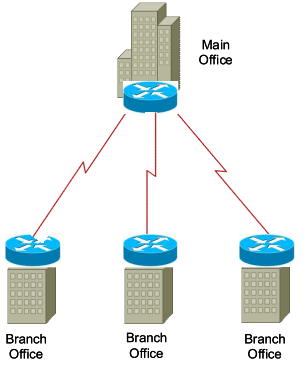
\includegraphics[scale=1]{figures/ex/cmo.png}
\caption{Connection to the Main Office}
\end{figure}

"\`E stata progettata una rete di una piccola compagnia con una topologia gerarchica \textit{Hub-And-Spoke}. La LAN in ogni ufficio secondario è connessa all'ufficio principale tramite un router ed un link con capacità $C = 128\ Kbps$. Dove $(1\ Kbit = 1000\ bits)$. In uno dei siti il flusso del traffico in uscita è generato principalmente da applicazioni CAD fino ad adesso. Per quel traffico, che può essere modellato come un processo di Poisson con rate $\lambda_0 = 3\ pkt/s$, è richiesto che il queueing delay nel router (per i pacchetti in coda) sia meno di $0.5$ secondi con probabilità più grande di $0.99$. A seguito di una nuova configurazione dei processi di business, è anche necessario installare un numero di computer per l'automazione degi uffici. Ci si aspetta che ognuno di loro generi un flusso di pacchetti verso l'ufficio centrale ad un average rate di $\lambda = 1\ pkt/s$. Per quest'ultimo flusso, è richiesto che l'average time speso nel router sia minore od uguale ad 1s.

Le dimensioni dei pacchetti possono essere modellate da variabili casuali indipendenti che sono esponenzialmente distribuite con valore medio $D = 500bytes$.

\begin{itemize}
\item Si assuma che la coda di output del router abbia capacità infinita e sia condivisa da tutti i flussi di traffico secondo disciplina di coda FCFS. Si determini il massimo numero $M$ di nuovi computer che possono essere installati;
\item Considerando il valore $M$, si valuti la \textit{packet loss probability} nel caso la dimensione della coda di output sia limitata a 10 pacchetti.
\end{itemize}

Abbiamo una topologia Hub-And-Spoke. (centro-e-raggi, topologia stellare). $C = 128\ Kbps$. Dove $(1\ Kbit = 1000\ bits) \implies C = 128000\ bit/s$. $\lambda_o = 3\ pkt/s\ \land\ \lambda = 1\ pkt/s$. Si richiede che il ritardo di accodamento nel router sia minore di $0.5s$ con probabilità maggiore di $0.99$. Le lunghezze dei pacchetti sono distribuite esponenzialmente di media 500 bytes. Politica FCFS. Quanto è il numero massimo di computer installabili $M$?

Supponiamo di indicare con $W$ la v.a. che rappresenta il ritardo di accodamento; il vincolo è il seguente, con $(\tau = 0.5s),\ \underline{s=threshold}=0.99$:

\[
	\Pr\{W < (\tau = 0.5s)\ |\ si\ faccia\ coda\} > (0.99 = s)
\]

Indichiamo con $\bar{R}$ il ritardo di accodamento per l'ultimo flusso. Deve valere: $\bar{R} \leq 1s$. Cerchiamo di risolvere il sistema con M/M/1. Abbiamo già delle ipotesi, ma dovremo farne di aggiuntive. Modelliamo quindi il router con un sistema a coda M/M/1:

Abbiamo un buffer output, ed un trasmettitore collegato in serie che è associato al link di uscita. Ipotesi: flusso secondo il quale arrivano i pacchetti di POISSON (pacchetti applicazioni CAD). Stiamo trascurando il ritardo di elaborazione router.
Capacità di elaborazione talmente elevata da ritenersi trascurabile (NO BOTTLENECK). Inoltre: $(d = +\infty)$. Il router opera con FCFS (quella contemplata dal sistema a coda M/M/1). Ipotesi aggiuntiva: certo numero di flussi, $M$ riguardanti i computer dell'Office Automation. Processo degli arrivi di POISSON. Ipotesi di indipendenza abbastanza scontata, dal momento che i vari utenti non si influenzeranno a vicenda. $M\lambda$. Ipotesi aggiuntiva: supponiamo che gli arrivi dei pacchetti relativi ai computer Office Automation siano indipendenti da quelli delle applicazioni CAD. Effettuando il POOLING, abbiamo che la distribuzione risultante è sempre un processo di POISSON con parametro dato dalla somma dei parametri: $\lambda' = \lambda_0+M\lambda$. Quindi $\lambda'$ è la velocità di arrivo dei clienti nel sistema a coda, $\mu$ è la velocità di servizio del router, ovvero il numero medio di pacchetti elaborati dal router per unità di tempo quando il router è costantemente occupato. Abbiamo dei tempi di servizio indipendenti, identicamente distribuiti ed indipendenti dai tempi di interarrivo. Nel sistema i tempi di servizio corrispondono ai tempi di trasmissione. Questo tempo di servizio è legato al parametro (valore medio) $D$ della distribuzione esponenziale che caratterizza la lunghezza dei pacchetti. Quindi abbiamo che il tempo medio di trasmissione è $\frac{1}{\mu} = \frac{D}{C} [s]$, ed abbiamo quindi $\mu = \frac{C}{D} = \frac{1}{D/C} = 32\  [pkt/s]$, ovvero abbiamo 32 pacchetti in media quando il router è costantemente occupato.

\begin{itemize}

\item{\textbf{Parte 1}}

Tutte le ipotesi del sistema a coda M/M/1 sono rispettate. Possiamo quindi utilizzarne i risultati: $\{\lambda',\mu\}$. Dobbiamo andare ad imporre quelle due condizioni. Per un M/M/1, il ritardo per cliente è $\bar{R} = \frac{1}{(\mu-\lambda)}$. Il ritardo per cliente è una v.a. distribuita esponenzialmente $\iff [R \sim EXP(\mu-\lambda)]$. Guardando adesso all'altra condizione, si dimostra che:

\[
	[F_W(y) = \Pr\{W \leq y\} = 1-\rho\e^{-\mu(1-\rho)y},\ y\geq 0]
\]

Tale è la CDF del Ritardo del cliente nella CODA! (Nella sola coda). $W$ sarebbe il tempo di permanenza del cliente nella SOLA coda del sistema a coda M/M/1. Distribuzione valutata su tutti i clienti (anche per quelli che non ci interessano). Dobbiamo condizionarla al fatto che si faccia coda. Quando $(y=0)$, esce $\Pr\{W\leq 0\} = (1-\rho)$. Ovvero la probabilità che il tempo di permanenza in fila di attesa sia nullo è pari a $(1-\rho)$. $\Pr\{W = 0\} = 1-\rho$. Si tratta di una v.a. mista. $\rho$ è il fattore di utilizzazione del router. Nel sistema a coda M/M/1, $\rho = (\frac{\lambda'}{\mu})$. Nell'M/M/1, $(1-\rho)=\pi_0^{(a)}$, ovvero la frazione di tempo a regime nel quale nel sistema a coda non vi sono clienti. La probabilità che il tempo di permanenza sia nullo è PARI alla probabilità che all'arrivo la fila di attesa SIA VUOTA!

\[
	[\Pr\{W = 0\} = 1-\rho = \pi_0]
\]

Questa è pari alla probabilità che un cliente AL SUO ARRIVO vada subito al router. In generale: $\pi_i^{(a)} \neq \pi_i$, laddove il primo membro della disuguaglianza riflette la visione dei clienti all'arrivo, valutata solo sugli istanti di arrivo, mentre il secondo membro riflette la visione all'esterno del sistema, considerando tutto l'asse temporale. $\pi_i$, ponendo l'ERGODICIT\`A, rappresenta la frazione di tempo nel quale vi sono $i$ clienti a regime. Mentre $\pi_i^{(a)}$ è la probabilità calcolata valutando SOLTANTO GLI ISTANTI DI ARRIVO! Frazione degli ARRIVI che trovano il sistema (a regime) nello stato $i$. Infatti potremmo avere ad esempio: $\{\{\pi_1 = \frac{1}{3},\ \pi_0=\frac{2}{3}\}\ \land\ \{\pi_0^{(0)}=1,\ \pi_1^{(0)}=0,\ \pi_2^{(0)}=0\}\}$.

\begin{thrm}{\textbf{P.A.S.T.A. \textit{POISSON ARRIVALS SEE TIME AVERAGES}}}

\[
	\left\{
	\begin{aligned}
	&\pi_i = \lim_{t\to\infty}{\Pr\{N(t)=i\}}\\
	&\pi_i^{(a)} = \lim_{t\to\infty}{\Pr\{N(t)=i\ |\ un\ arrivo\ subito\ dopo\ t\}}
	\end{aligned}
	\right.
\]

Se gli arrivi dei clienti si susseguono con processo di POISSON, abbiamo che: $\pi_i^{(a)}=\pi_i,\ \bar{N}=\sum_{i=0}^\infty{i\pi_i}$

\end{thrm}

Dove la prima equazione è una quantità calcolata sull'insieme delle realizzazioni. (Media di insiemi). Ma se vale L'ERGODICIT\`A, allora le medie d'insieme coincidono con le medie TEMPORALI. $\pi_i$ rappresenta la frazione del tempo nella quale vi sono a regime $i$ clienti nel sistema; $\pi_i^{(a)}$ rappresenta la frazione dei clienti che, all'arrivo trovano il sistema nello stato $i$. Coincide con la probabilità (a regime), che all'arrivo un cliente trovi $i$ clienti nel sistema. Rappresenta cosa vedono i clienti all'arrivo.

Per i nostri scopi, $[\pi_0^{(a)} = \Pr\{W = 0\}] = [\underline{1-\rho = \pi_0}]$, ove la parte sottolineata è la probabilità che vi siano 0 clienti, in un istante qualsiasi, mentre il primo membro è la probabilità che un cliente, al suo arrivo, trovi 0 clienti nel sistema. Grazie al teorema appena visto, esse coincidono. 

$\rho$ è la frazione del tempo in cui il router è occupato $\implies$ probabilità che il router sia occupato. $(1-\rho)$ è la probabilità che il router sia quindi libero. 
$\Pr\{W \leq \tau\ |\ si\ fa\ coda\} = (\dots)$ è la probabilità che il tempo di permanenza in FILA DI ATTESA sia inferiore (od uguale) a $\tau$, quando si fa coda.
Quindi abbiamo:

\[
	(\dots) = 1-\Pr\{W > \tau\ |\ si\ fa\ coda\} = 1-\frac{\Pr\{W > (y := \tau),\ si\ fa\ coda\}}{\Pr\{si\ faccia\ coda\}} = (\dots)
\]

Notiamo che $\{W > y\} \supseteq \{si\ fa\ coda\}$, ed inoltre, dal teorema appena visto (PASTA) vale che: $1-\pi_0^{(a)} = 1-\pi_0 = \rho = \Pr\{si\ fa\ coda\}$, ovvero la probabilità che all'arrivo di un cliente il servitore sia occupato coincide con la probabilità di fare coda. Ciò implica: $\implies$

\[
	(\dots) = 1-\frac{\Pr\{W>\tau\,\ si\ fa\ coda\}}{\Pr\{si\ fa\ coda\}} = 1-\frac{\Pr\{W\geq\tau\}}{\rho} =
\]
\[
	= 1-\frac{\rho\e^{-\mu(1-\frac{\lambda}{\mu})y}}{\rho} = 1-\e^{-\mu(1-\frac{\lambda}{\mu})y},\ y\geq 0
\]

Concludiamo che:

\[
	\Pr\{W \leq y\ |\ si\ fa\ coda\} = 1-\e^{-\mu(1-\frac{\lambda}{\mu})y} \iff W|_{\{si\ fa\ coda\}} \sim EXP(\mu-\lambda)
\]

quindi nell'M/M/1, $R=W|_{\underline{\{si\ fa\ coda\}}}$. Si riferisce proprio alla medesima distribuzione esponenziale, con il medesimo parametro!

Consci che $[R = \frac{1}{\mu-\lambda'}]$, allora procediamo:

\[	
	1-\e^{-(\mu-\lambda')\tau} > s \implies \e^{-(\mu-\lambda')\tau} < (1-s) \implies -(\mu-\lambda')\tau < \log(1-s) \implies (\dots)
\]
\[
	(\dots) \implies -\mu\tau +\lambda'\tau < \log(1-s) \implies [\lambda'\tau < \log(1-s)+\mu\tau] \implies (\dots)
\]
\[
	(\dots) \implies \lambda_0+M\lambda < \frac{\log(1-s)}{\tau} + \mu \implies M\lambda < \mu + \frac{\log(1-s)}{\tau}-\lambda_0 \implies (\dots)
\]
\[
	(\dots) \implies M < \frac{1}{\lambda}[\mu+\frac{1}{\tau}\log(1-s)-\lambda_0] = [32.8]
\]

ove il valore si è ottenuto appositamente sostituendovi i dati al secondo membro dell'ultima disequazione.

Quindi $\floor{M} = M_{max} = 32$ computer massimi.
Si ottiene $M \leq 32.8$, quindi possiamo installare MASSIMO 32 COMPUTER. D'altro canto dobbiamo rispettare anche il vincolo sull'average router time:

\[
	\bar{R} = \frac{1}{\mu-\lambda'} \implies \frac{1}{\mu-\lambda'} \leq 1s \implies ((\mu-\lambda')>0) \geq 1s \implies (\dots)
\]

ove l'ultima parentesizzazione maggiore di 0 indica la condizione di STABILIT\`A, che naturalmente deve essere sempre rispettata.

\[
	(\dots) \implies \mu - (\lambda_0+M\lambda)\geq 1 \implies \mu-\lambda_0 -M\lambda \geq 1 \implies M\leq\frac{\mu-\lambda_0-1}{\lambda} =
\]
\[
	= \frac{1}{\lambda}[\mu-\lambda_0-1] \implies M\leq 28
\]

Ne si conclude che $M_{max}=\min{\{28,32\}} = 28$ computer. Quindi: $\underline{\underline{[M\leq M_{max}=28]}}$.


\newpage

\item{\textbf{Parte 2}}: 

\subsubsection{M/M/1/k}

Consideriamo che $d = 10\ pkt$ (10 pacchetti), $d<+\infty$ ed abbiamo quindi un buffer di dimensione finita. $\iff (d=10)<+\infty$. In questo caso NON possiamo studiare il sistema con un modello M/M/1! Ci serve invece un \textit{M/M/1/k}, nel quale la dimensione del buffer è limitata. Pensiamo a $k$ come la capacità di tutto il sistema (includendo il centro di servizio). Stiamo quindi considerando un sistema a CODA CON PERDITA. Quando un elemento arrivando trova la coda piena, il sistema interviene con il meccanismo di DISCARD (avviene il fenomeno \textit{packet loss}). In questo caso $\lambda'$ è la velocità di arrivo dei clienti al sistema (POISSON). $\lambda_s$ sarà sempre la velocità di ingresso alla coda e di uscita (numero medio di clienti). $\rho=\frac{\lambda_s}{\mu}$ è il fattore di utilizzazione del servitore. Abbiamo che:

\[
	\Pr\{perdita\} = \frac{\lambda^l}{\lambda'} = \pi_k^{(a)} = \pi_k
\]

grazie a PASTA. Disegnamo il relativo DTT della catena:

\begin{center}
\begin{tikzpicture}[->, >=stealth', auto, semithick, node distance=2cm]
\tikzstyle{every state}=[fill=white,draw=black,thick,text=black,scale=1]
\node[state]    (0)                     {$0$};
\node[state]    (1)[right of=0]   {$1$};
\node[state]    (2)[right of=1]   {$2$};
\node[state] (d) [right of=2] {\ldots};
\node[state]    (km1)[right of=d]   {$k-1$};
\node[state]    (k)[right of=km1]   {$k$};
\path
(0) edge[bend left]     node{$\lambda'$}         (1)
(1) edge[bend left]     node{$\lambda'$}         (2)
    edge[bend left,below]    node{$\mu$}            (0)
(2) edge[bend left]     node{$\lambda'$}           (d)
    edge[bend left,below]    node{$\mu$}             (1)
(d) edge[bend left]         node{$\lambda'$}   (km1)
	edge[bend left,below]   node{$\mu$}          (2)
(km1) edge[bend left]       node{$\lambda'$}  (k)
	  edge[bend left,below]   node{$\mu$}     (d)
(k)   edge[bend left,below]  node{$\mu$}          (km1);
\end{tikzpicture}
\end{center}

Sia $N(t)$ il numero di clienti nel sistema a tempo $t$. 
$\Pr\{\phi_i(t) > \tau\} = (\dots)$, dove $\phi_i(t)$ indica il tempo di soggiorno residuo nello stato $i$ al tempo $t$, indica la probabilità che per almeno $\tau$ unità di tempo non ci sia alcun arrivo e NON vi sia la fine del servizio in corso, condizionata con il fatto che attualmente vi sono $i$ clienti nel sistema.

Indichiamo con $\xi_{Rt} \sim EXP(\lambda')$ la v.a. tempo di interarrivo residuo al tempo $t$, e con $\eta_{Rt} \sim EXP(\mu)$ la v.a. tempo di servizio residuo al tempo $t$. Tutte indipendenti ed indipendenti tra di loro, grazie all'ipotesi di (inter)-indipendenza. 

\[
	(\dots) = \Pr\{\xi_{Rt}>\tau,\ \eta_{Rt}>\tau\} = \Pr\{\xi_{Rt}>\tau\}\Pr\{\eta_{Rt}>\tau\} = \e^{-\lambda'\tau}\e^{-\mu\tau} = \e^{-(\lambda'+\mu)\tau}
\]

Quindi abbiamo di nuovo: $-q_{ii} = \mu+\lambda' \implies$

\[
	\tau_{i,i+1} = \frac{q_{i,i+1}}{-q_{ii}} = \frac{q_{i,i+1}}{(\mu+\lambda')}
\]

$\tau_{i,i+1}$ è la probabilità che lasciando lo stato $i$, il processo vada verso $i+1$. Sfruttando il teorema delle probabilità totali nel continuo, abbiamo: $q_{i,i+1} = (\mu+\lambda') \frac{\lambda'}{(\mu+\lambda')} = \lambda'$. Quindi sarà $\lambda'$ fino a $k-1$. La CMTC è una catena omogenea, IRRIDUCIBILE e dal momento che $\cardinality{stati}<+\infty \implies$ allora essa è SICURAMENTE ERGODICA! CATENA SEMPRE ERGODICA. Sistema STABILE.

\[
	\left\{
	\begin{aligned}
	&[\pi_i = \pi_0(\frac{\lambda'}{\mu})^i]\\
	&[\pi_0 = \frac{1}{1+\sum_{i=1}^k{(\frac{\lambda'}{\mu})^i}}]
	\end{aligned}
	\right.
\]

$i=1,2,\ \dots,\ k$.

Notiamo che:

\[
	\sum_{i=0}^k{\rho^i} = \left\{
	\begin{aligned}
	&k+1,\ \rho=1\\
	&\frac{1-\rho^{k+1}}{(1-\rho)},\ p\neq 1
	\end{aligned}
	\right.
\]

Quindi nel nostro caso abbiamo:

\[
	\pi_0 = \frac{1}{\sum_{i=0}^k{\rho^i}} = \frac{1}{\frac{1-\rho^{k+1}}{(1-\rho)}} = \frac{1-\rho}{1-\rho^{k+1}}
\]

Quindi abbiamo come Distribuzione di regime:

\[
	\pi_i = \frac{1-\rho}{1-\rho^{k+1}} \rho^i,\ i=0,1,2,\ \dots,\ k
\]

Si noti che vale anche per $i=0$. Allora:

\[
	[\Pr\{perdita\} = \underline{\pi_k^{(a)} \stackrel{PASTA}{=} \pi_k} = [\frac{1-\rho}{1-\rho^{k+1}} \rho^k]]
\]

da valutarsi con $k=10+1=d+1<+\infty$, in quanto include anche il centro di servizio.
Facendo i calcoli esce $0.07 \implies (70\%)$.

La probabilità di perdita si poteva trovare, come precedentemente enunciato, anche effettuando il rapporto $\frac{\lambda_L}{\lambda'}$. Banalmente, per SPLITTING si ha: $[\lambda_L=\lambda'-\lambda_S]$. Le perdite comunque mi fanno venire meno la caratteristica di POISSON.

\[
	\Pr\{k\ arrivi\ in\ \tau\} = \frac{(\lambda\tau)^k}{k!}\e^{-\lambda\tau}
\]

ma la sequenza degli ingressi a valle della diramazione NON è più di POISSON! $\rho = (\frac{\lambda_S}{\mu})$ rappresenta il fattore di utilizzazione, quindi la frazione del tempo a regime in cui il servitore è occupato. $\rho=1-\pi_0 \implies \pi_0=1-\rho$.

$\lambda_S=\mu(1-\pi_0)$ rappresenta la velocità delle partenze (\textit{departure}) dei clienti dal mio sistema. Abbiamo: $[\pi_0 = \frac{1-\rho}{1-\rho^{k+1}}]$.

\[
	\lambda_L = \lambda'-\lambda_S = \lambda'-\mu(1-\pi_0)
\]

Quindi $\lambda_S$ è la velocità secondo la quale i clienti partono dal sistema, od anche la media dei clienti che partono all'unità di tempo. Guardando il DTT, vi è una partenza quando FINISCE un servizio! Determinando le frequenze delle transizioni a sinistra, potremo sapere le frequenza delle partenze. La frequenza delle partenze si ottiene sommando tutte le frequenze delle transizioni $\pi_iq_{ij}$, sfruttando opportunamente l'inversa della CONDIZIONE DI \underline{NORMALIZZAZIONE}:

\[
	\pi_1\mu + \pi_2\mu +\ (\dots)\ +\pi_k\mu = \mu\sum{\pi_i} = [\lambda_S = \mu(1-\pi_0)]
\]

Stessa cosa mettendoci a valle della diramazione ed a monte della coda: (ARRIVI DI CLIENTI dall'esterno del sistema). $\lambda_S$ rappresenta qui il numero medio di clienti che entrano nel sistema per unità di tempo.

\[
	\lambda_S = [\pi_0\lambda'+\pi_1\lambda'+\ \dots\ +\pi_{k-1}\lambda'] = \lambda'
\]

Valgono le equazioni di bilanciamento locale, valide solo per una CMTC di nascita e morte (BDCMTC):

\[
	\pi_1\mu = \pi_0\lambda' \implies \pi_{k+1}\mu = \pi_k\lambda'
\]

ovvero le sommatorie sono identiche.

$\frac{\lambda_L}{\lambda'}$ rappresenta la probabilità di perdita.

\begin{thrm}{\textbf{Probabilità di perdita}}

\[
	\Pr\{perdita\} = \frac{1-\rho}{1-\rho^{k+1}}\rho^k = \pi_k^{(a)} = \pi_k
\]

ove $\pi_k$ rappresenta la probabilità che il sistema si trovi nello stato $k$ in un istante qualsiasi. Abbiamo anche:

\[
	\Pr\{perdita\} = \frac{(\lambda_L = \lambda'-\lambda_S)}{\lambda'} = 1-\frac{\lambda_S}{\lambda'} = (\dots)
\]
\end{thrm}

Ove $\lambda_S$ è stato trovato applicando Little al primo sottosistema, ottenendo quindi $\lambda_S =\mu(1-\pi_0)$.

\begin{proof}

\[
	(\dots) = 1-\frac{\mu(1-\pi_0)}{\lambda'} = 1-\frac{1}{\rho}(1-\frac{1-\rho}{1-\rho^{k+1}}) = 1-\frac{1}{\rho}(\frac{1-\rho^{k+1}-1+\rho}{1-\rho^{k+1}})
\]
\[
	1-\frac{1}{\rho}\rho \frac{(1-\rho^k)}{(1-\rho^{k+1})} = \frac{1-\rho^{k+1}-1+\rho^k}{1-\rho^{k+1}} = \frac{\rho^k(1-\rho)}{(1-\rho^{k+1})};
\]

\end{proof}

La probabilità di perdita di un cliente deve quindi alla fine coincidere con il rapporto $\frac{\lambda_L}{\lambda'}$.

\end{itemize}

\subsection{Sistemi a coda M/M/m}

Il sistema a coda M/M/m rappresenta una generalizzazione del sistema M/M/1. Abbiamo $m$ router.
Anche in questo caso, il processo degli arrivi è un processo di POISSON con velocità $\lambda$. ($\lambda$ = velocità di arrivo dei clienti). In media arrivano $\lambda$ clienti per unità di tempo. Anche in questo caso i tempi di servizio sono v.a. indipendenti (mutuamente), i.d. con una distribuzione esponenziale negativa unilatera, con tempo medio di servizio $(\frac{1}{\mu})$, ed indipendenti statisticamente dai tempi di interarrivo dei clienti nel sistema a coda. La velocità del centro di servizio sarà variabile (il centro di servizio include ora $m$ servitori), ovvero dipende dal numero di router attivi in un certo istante di tempo. Se $i$ è il numero di clienti nel sistema a coda in un certo istante di tempo, $i<m \implies i\mu$ velocità del centro di servizio. $i$ sono i clienti IN TUTTO IL SISTEMA! In totale quindi i servitori attivi serviranno $i\mu$ utenti $\forall$ unità di tempo. $i\geq m$ tutti gli $m$ servitori saranno attivi $\implies$ velocità $m\mu$. Quindi $i\geq m$ centro di servizio alla massima velocità possibile. $m\mu$ = capacità TOTALE DI SERVIZIO DEL SISTEMA (del centro di servizio). Come nella M/M/1, la dimensione del buffer e la popolazione sono illimitate ($\iff d,e<+\infty$). Disciplina di queueing di default (FCFS). Modellabile come uno stack FIFO. Se arriva un cliente e c'è un certo numero di router liberi, sarà assegnato in maniera random ad uno di questo. Approccio MARKOVIANO basato sul processo stocastico che si riferisce al numero di clienti nell'intero sistema a coda al tempo $t$, ovvero $N(t)$. La sua evoluzione sarà determinata dalle v.a. tempi di interarrivo e tempi di servizio. Dato che per queste ipotesi queste v.a. sono prive di memoria e statisticamente indipendenti $\implies$ siamo dinanzi una CMTC, il cui diagramma dei tassi di transizione è il seguente:

\begin{center}
\begin{tikzpicture}[->, >=stealth', auto, semithick, node distance=2cm]
\tikzstyle{every state}=[fill=white,draw=black,thick,text=black,scale=0.8]
\node[state]    (0)                     {$0$};
\node[state]    (1)[right of=0]   {$1$};
\node[state]    (2)[right of=1]   {$2$};
\node[state] (d) [right of=2] {\ldots};
\node[state]    (mm1)[right of=d]   {$m-1$};
\node[state]    (m)[right of=mm1]   {$m$};
\node[state]    (mp1)[right of=m]   {$m+1$};
\node[state]    (mp2)[right of=mp1]   {$m+2$};
\node[state]    (d2)[right of=mp2]  {\ldots};

\path
(0) edge[bend left]     node{$\lambda$}         (1)
(1) edge[bend left]     node{$\lambda$}         (2)
    edge[bend left,below]    node{$\mu$}            (0)
(2) edge[bend left]     node{$\lambda$}           (d)
    edge[bend left,below]    node{$2\mu$}             (1)
(d) edge[bend left]         node{$\lambda$}   (mm1)
	edge[bend left,below]   node{$3\mu$}          (2)
(mm1) edge[bend left]       node{$\lambda$}  (m)
	  edge[bend left,below]   node{$(m-1)\mu$}     (d)
(m)   edge[bend left]   node{$\lambda$}      (mp1)
      edge[bend left,below]  node{$m\mu$}          (mm1)
(mp1) edge[bend left]       node{$\lambda$}  (mp2)
	 edge[bend left,below]   node{$m\mu$}      (m)
(mp2) edge[bend left]       node{$\lambda$}   (d2)
      edge[bend left,below] node{$m\mu$}    (mp1)
(d2) edge[bend left,below]   node{$m\mu$}     (mp2);
\end{tikzpicture}
\end{center}

CMTC nascita e morte (BDCMTC), con $\cardinality{stati}=+\infty$ (infiniti), fila di attesa di dimensione illimitata. Tassi di nascita pari a $\lambda$, tassi di morte $m\mu$, che sarebbe il tasso di morte nello stato $i$ prima che si saturino i servitori disponibili, dopodiché $(i\geq m)$, sempre pari a $m\mu$.

\subsubsection{Calcolo dei tassi (velocità) di transizione}

Supponiamo $N(t)=i\neq 0$ ($i$ clienti nel mio intero sistema a coda), ovvero qualsiasi stato diverso dallo stato banale. Il successivo cambiamento di stato sarà legato od all'arrivo di un nuovo cliente od al completamento di uno dei servizi eseguiti in parallelo al tempo $t$. Comunque abbiamo $i$ clienti totali. Possibili casi: $\{i++,\ i--\}$. L'intervallo di tempo da $t$ al successivo arrivo lo indichiamo con $\underline{\xi_R(t) \sim EXP(\lambda)}$, ovvero il tempo di interarrivo residuo (stessa caratteristiche dei tempi di interarrivo). Il tempo che passa tra l'istante presente $t$ ed il successivo completamento del servizio, sarà $\eta_R(t)$, e sarà pari al minimo dei tempi di servizio residui in $t$. Ci saranno un certo numero di servizi. $\eta_R(t) = \min{\{...\}}$, ovvero al minimo dei tempi di servizio residui legati a quei servizi che al tempo $t$ stanno procedendo in parallelo. Quando $i<m$, ci saranno $i$ servizi che stanno procedendo in parallelo. Anche i tempi di servizio residui sono \underline{indipendenti} fra di loro per ipotesi, dal momento che i servizi procedono in parallelo senza influirsi. Quindi $\eta_R(t) \sim EXP(\sum_i{\mu_i})$. Quando $i<m\implies$ $\eta_R(t) \sim EXP(i\mu)$. Se invece $i\geq m$, $\eta_R(t) \sim EXP(m\mu)$. A questo punto, il tempo che passa dall'istante presente $t$ e la successiva transizione di stato, sarà $\phi_i(t)$ (tempo di soggiorno residuo nello stato $i$ al tempo $t$) prima di cambiare stato $\implies$

\[
	\phi_i(t) = \min{\{\xi_R(t),\ \eta_R(t)\}} \implies \phi_i(t) \sim EXP(-q_{ii})
\]

ove l'ultima implicazione è valida grazie al fatto che queste variabili casuali sono i.i.d. ed indipendenti tra di loro. Abbiamo:

\[
	-q_{ii} = \left\{
	\begin{aligned}
	&(\lambda+i\mu),\ i<m\\
	&(\lambda+m\mu),\ i\geq m
	\end{aligned}
	\right.
\]

(Velocità totale di uscita \underline{dallo stato i}). Parametro $-q_{ii}$. Quindi, quella quantità rappresenta con che velocità in totale esco dallo stato. Ma se $\underline{i<m}$, perché $q_{i,i+1} = \lambda,\ q_{i,i-1}=i\mu$. Solito giochetto. (Se $i\geq m,\ q_{i,i-1}=m\mu$). Consideriamo:

\[
	\tau_{i,i+1} = \frac{q_{i,i+1}}{-q_{ii}} = \Pr\{\xi_R(t) < \eta_R(t)\} = (\dots)
\]

ove l'ultima quantità rappresenta la probabilità che il prossimo arrivo preceda la fine del servizio (il completamento del servizio). Dobbiamo quindi applicare il teorema delle probabilità totali nel continuo, ottenendo alla fine:

\[
	(\dots) = \left\{
	\begin{aligned}
	&\frac{\lambda}{\lambda+i\mu},\ i<m\\
	&\frac{\lambda}{\lambda+m\mu},\ i\geq m
	\end{aligned}
	\right.
\]

CMTC OMOGENEA, IRRIDUCIBILE, ma non sappiamo tuttavia se è ERGODICA.

\[
	\left\{
	\begin{aligned}
	&[\pi_0 = \frac{1}{1+\sum_{i=1}^{m-1}{(\frac{\lambda}{\mu})^i\frac{1}{i!}} + (\frac{m^m}{m!})\sum_{i=m}^\infty{(\frac{\lambda}{m\mu})^i}}]\\
	&\left\{
	\begin{aligned}
	&\pi_i = \pi_0 (\frac{\lambda}{\mu})^i \frac{1}{i!},\ i<m\\
	&\pi_i = \pi_0 (\frac{\lambda}{\mu})^i \frac{1}{m!m^{i-m}},\ i\geq m
	\end{aligned}
	\right.
	\end{aligned}
	\right.
\]

Dobbiamo capire qual'è la CONDIZIONE MAX di ERGODICIT\`A (si ha una condizione di regime). La sommatoria ad infiniti termini (serie) a denominatore di $\pi_0$ deve convergere di nuovo. La condizione di ERGODICIT\`A è quindi: $(\frac{\lambda}{m\mu}) < 1$ (convergenza della serie geometrica). Quando $\rho := \frac{\lambda}{m\mu} < 1$ questa sommatoria (serie) converge, e si ha una distribuzione che è quella di regime. $[\lambda < m\mu]$ è proprio la condizione di STABILIT\`A, la quale indica che la velocità di arrivo deve essere minore della capacità totale di servizio. Serve sostanzialmente per evitare l'"ingolfamento". $\rho$ è il fattore di utilizzazione del generico router (Non del centro di servizio). Ognuno dei router avrà un fattore di utilizzazione pari a $\rho$, quando il carico è EQUAMENTE DISTRIBUITO. $\frac{\lambda}{m}$ sarà la capacità di arrivo del singolo cliente. Servono in media lo stesso numero di clienti $\forall$ unità di tempo. Tutti lavoreranno alla stessa maniera. Ogni router si vedrà arrivare quindi $\frac{\lambda}{m}$ clienti per unità di tempo. Fattore di utilizzazione; frazione di tempo quando il servitore è occupato. Infatti, applicando \underline{Little} troviamo: $(\frac{\lambda}{m})(\frac{1}{\mu})$, trovando la frazione di tempo nel quale il router è occupato per unità di tempo nella quale il router è costantemente occupato, quando il carico di lavoro è EQUAMENTE DISTRIBUITO. $\frac{\lambda}{\mu}$ è l'\textit{intensità di traffico} (arrivano $\lambda$ clienti, $\frac{1}{\mu}$ è il lavoro medio richiesto dal cliente). Quindi sfruttiamo ancora Little e troviamo: $\lambda(\frac{1}{\mu})$, trovando così il \underline{\underline{CARICO MEDIO DI LAVORO}}. 

\[	
	[\frac{\lambda}{\mu} = m(\rho := \frac{\lambda}{m\mu}) = m\rho]
\]

Si usi questo fatto per vedere a cosa converge la sommatoria geometrica:

\[	
	[\pi_0 = \frac{1}{\sum_{i=0}^{m-1}{(m\rho)^i \frac{1}{i!}} + (\frac{m^m}{m!} \frac{\rho^m}{1-\rho} = \frac{(m\rho)^m}{m!(1-\rho)})}]
\]

e tramite questa espressione possiamo ovviamente trovare le $\pi_i$.

ERGODICIT\`A se: $[\underline{\lambda < m\mu}]$. Abbiamo trovato la distribuzione di regime. Nel caso M/M/1, abbiamo poi ricavato tutti i numeri medi di clienti e tempi di servizio, etc. Nel caso M/M/1 siamo partiti da $\bar{N}$.

\subsubsection{Quantità medie tipiche}

Adesso partiamo da $\bar{T}$, ovvero il ritardo medio per cliente a regime. Terminologia tempo di risposta. $\bar{T}$ tempo di risposta. Tempo di permanenza del cliente nel sistema a coda. Abbiamo:

\[
	(\bar{T} := \E[T]) = \E[t_s] + \E[W] = \frac{1}{\mu} + (\dots)
\]

ove $W$ è il tempo di accodamento, ovvero il queueing delay. Adesso per valutare il tempo medio di permanenza in fila di attesa utilizziamo il concetto di \textit{MEDIA CONDIZIONATA}:

\[
	(\dots) = \E[\E[W\ |\ k\ clienti\ all'arrivo]] = \mathord{\cdot}(k)
\]

dove $\{k\ clienti\ all'arrivo\}$ sarebbe l'evento nel quale troviamo $k$ clienti all'arrivo in testa al sistema. Tempo di permanenza, sapendo che all'arrivo il cliente trova $k$ clienti nel sistema. Quindi:

\[
	\bar{T} = \frac{1}{\mu} + \sum_{k=m}^\infty{\E[W\ |\ k\ clienti\ all'arrivo]}\pi_k^{(a)}
\]

Notiamo che $k$ parte da $m$, perché se $k<m$ quella quantità sarebbe nulla!
Il tempo medio di permanenza nella fila di attesa è nullo quindi se $k<m$! Se arrivato nel sistema a coda trovo un numero $(k<m)$ di clienti, allora VADO DIRETTAMENTE nel CENTRO DI SERVIZIO! Sommatoria che parte da $m$ quindi. Volendo la si potrebbe fare partire da 0, senza alcuna perdità di generalità, dal momento che i primi $(m-1)$ termini sarebbero comunque nulli. Abbiamo:

\[	
	\bar{T} = \frac{1}{\mu} + \sum_{k=m}^\infty{\frac{k-m+1}{m\mu}(\pi_k^{(a)}=\pi_k)} = (\dots)
\]

Dove l'uguaglianza tra parentesi deriva da PASTA. Abbiamo sfruttato il fatto che: $[\E[W|k] = \frac{k-m+1}{m\mu}]$. Siamo nel caso $k\geq m$, ove vi sono $m$ clienti al servizio, $(k-m)$ clienti in fila di attesa ed io. Dopo che vi sarà il completamento di $(k-m)$ servizi mi troverò in testa alla fila di attesa. Ma dovrò quindi attendere il completamento di un ulteriore servizio (ecco perché il termine $+1$). Ma il tempo tra il completamento del servizio corrente ed il successivo è $(\frac{1}{m\mu})$! ($\leftarrow$ tempo medio di servizio). $\implies$

\[
	(\dots) = \frac{1}{\mu} + \sum_{k=m}^\infty{(\frac{k-m+1}{m\mu})\pi_0\frac{m^m}{m!}\rho^k} = \frac{1}{\mu} + \pi_0\frac{m^m}{m!}\sum_{k=m}^\infty{\frac{k-m+1}{m\mu}\rho^k} = (\dots)
\]

A questo punto possiamo porre: $i := k-m+1$, ed otteniamo:

\[
	(\dots) = \frac{1}{\mu} + \pi_0\frac{m^m}{m!m\mu}\sum_{i=1}^\infty{i(\rho^{i-1+m} = \rho^{i-1}\rho^m)} =
\]
\[
	= \frac{1}{\mu} + \frac{(m\rho)^m}{m!m\mu}\pi_0\sum_{i=1}^\infty{i\rho^{i-1}} = [\frac{1}{\mu} + \frac{\pi_0(m\rho)^m}{m!m\mu} \frac{1}{(1-\rho)^2}]
\]

Abbiamo quindi trovato il RITARDO MEDIO PER CLIENTE. Volendo potremmo anche trovare con Little: $\bar{N}=\lambda\bar{T} = (\dots)$. Spesso in letteratura si esprime $\bar{T}$ in funzione della probabilità di attesa:

\[
	\Pr\{accodamento\ (queueing)\} = \sum_{k=m}^\infty{(\pi_k^{(a)}=\pi_k)}
\]

sarebbe ovvero la sommatoria di queste probabilità. Si deriva quindi la \textit{C di ERLANG}. (La B di ERLANG è invece collegata alla probabilità di perdita (M/M/m/0)). 

Siamo in un sistema a coda M/M/m. Ritardo medio per cliente:

\[
	\left\{
	\begin{aligned}
	&\bar{T} = \frac{1}{\mu} + \frac{\pi_0(m\rho)^m}{m!m\mu} \frac{1}{(1-\rho)^2}\\
	&\rho = \frac{\lambda}{m\mu},\ \rho<1
	\end{aligned}
	\right.
\]

ove l'ultima equazione del sistema indica la condizione di \underline{STABILIT\`A}. Questa quantità ($\bar{T}$), viene solitamente espressa in letteratura in funzione della probabilità di ATTESA, nella quale dobbiamo considerare la situazione in cui abbiamo almeno $m$ clienti nel sistema a coda quando arriva un cliente:

\[
	\Pr\{queueing\} = \sum_{k=m}^\infty{(\pi_k^{(a)}=\pi_k)} = \sum_{k=m}^\infty{\pi_k} =
\]
\[
	\sum_{k=m}^\infty{\pi_0(\frac{\lambda}{m\mu} = \rho)^k \frac{m^m}{m!}} = \pi_0\frac{m^m}{m!}\sum_{k=m}^\infty{\rho^k} = (\dots)
\]

Siamo dinanzi una sommatoria geometrica, quindi:

\[
	(\dots) = \pi_0\frac{m^m}{m!} (\frac{\rho^m}{1-\rho}) = \frac{\pi_0(m\rho)^m}{m!(1-\rho)} := C(m,\frac{\lambda}{\mu})
\]

Abbiamo ottenuto quest'espressione $C(m,(\frac{\lambda}{\mu}))$, nota come funzione \textit{C di ERLANG} con parametro: $\{m,(\frac{\lambda}{\mu})\}$. Ci sono delle tabelle per questa formula. Abbiamo ricavato un modello per la M/M/m. Possono essere utilizzate per modellare quei sistemi di servizio che prevedono diverse risorse. Sistemi di servizio con un certo numero di risorse, corrispondenti ai router $(m)$, laddove $(i\geq m \implies\ queueing)$.

Modello M/M/m. Dobbiamo però ritrovare le ipotesi dietro all'M/M/m nel mondo reale. Call-center ad esempio. Processo secondo il quale si susseguono gli arrivi al sistema a coda dev'essere ben modellabile come un processo di POISSON. Durata media delle telefonate (tempi medi di servizio) $(\frac{1}{\mu})$. In un call center mi ritrovo queste ipotesi. Ci vorrebbero anche le ipotesi sulla dimensione del buffer e della popolazione. $(d,e = +\infty)$. Dimensionamento del numero massimo di operatori (servitori) in base ad un predeterminato massimo valore da non scavalcare relativo alla probabilità di accodamento. $\{\lambda,\frac{1}{\mu}\} \to m$. Problema di progetto. Potremo anche voler affrontare un problema di ANALISI. Durata media delle telefonate $(\frac{1}{\mu})$. [ANALISI $\rightarrow$ PROGETTO]. In funzione della C di ERLANG, troviamo il valore del ritardo medio per cliente:

\[
	\bar{T} = \frac{1}{\mu} + C\frac{1}{m\mu}(\frac{1}{1-\rho}),\ \rho<1
\]

Ricordiamo che $(C\ di\ ERLANG = \Pr\{queuing\})$. Adesso, noto il valore del ritardo medio per cliente, applico Little e trovo:

\[
	\bar{N} = \lambda\bar{T} = \frac{\lambda}{\mu} + C\frac{\lambda}{m\mu}(\frac{1}{1-\rho}) = [m\rho + C\rho(\frac{1}{1-\rho})]
\]

Troviamo ora il tempo medio di permanenza nella sola fila di attesa, dove $(\rho := \frac{\lambda}{m\mu})$:

\[
	\bar{W} = \bar{T} - (T_s = \frac{1}{\mu}) = C\frac{1}{m\mu}(\frac{1}{1-\rho})
\]

E adesso il numero medio di clienti nella sola fila di attesa, $\bar{N_q}$

\[
	[\bar{N_q} = \lambda\bar{W} = C\rho(\frac{1}{1-\rho})]
\]

Dove abbiamo nuovamente applicato Little al sottosistema costituito dalla sola fila di attesa. Ora passiamo al centro di servizio, ragionando con gli stessi argomenti:

\[
	\left\{
	\begin{aligned}
	&(T_s=\frac{1}{\mu})\\
	&\bar{N_s} = m\rho := \frac{\lambda}{\mu} = \lambda(\frac{1}{\mu})
	\end{aligned}
	\right.
\]

$\rho$ è il FATTORE DI UTILIZZAZIONE. A REGIME $(\rho<1)$. Ricordiamo che $\lambda$ è sempre la velocità di arrivo.

\subsubsection{Confronto tra tre sistemi MARKOVIANI}

Questi tre sistemi MARKOVIANI hanno la stessa capacità di servizio e stessa velocità tutti tra di loro:

\begin{itemize}

\item{1)}: Un singolo sistema M/M/1 con velocità di arrivo $m\lambda$ e velocità di servizio del singolo servitore pari a $m\mu$. Parametri: $\{m\lambda,m\mu\}$;
\item{2)}: $m$ code M/M/1, ogni coda con velocità di arrivo $\lambda$ e di servizio $\mu \implies\ \{m\lambda,m\mu\}$ come parametri;
\item{3)} Sistema M/M/m con velocità di arrivo $m\lambda$ ed $m$ servitori. Ricordiamo che qui vale:

\[
	[\frac{1}{\mu} + C\frac{1}{m\mu}(\frac{1}{1-\rho}) = \bar{T},\ (\rho<1)]
\]

Abbiamo parametri: $\{m\lambda,m\mu\}$.

\end{itemize}

Tre sistemi che hanno tutti la stessa velocità di arrivo e di servizio. Confrontiamo i ritardi medi di permanenza per i clienti. Dobbiamo quindi stilare una graduatoria:
Effettuiamo un confronto:

\[
	\left\{
	\begin{aligned}
	&\bar{T_1} = \frac{1}{m\mu-m\lambda} = \frac{1}{m(\mu-\lambda)}\\
	&\bar{T_2} = \frac{1}{\mu-\lambda}\\
	&\bar{T_3} = ?
	\end{aligned}
	\right.
\]

Dovremmo fare i conti con l'espressione di $\bar{T}$ precedentemente trovata. Ma, intuitivamente la classifica sarebbe: $\{1,3,2\}$. Il primo sarebbe il migliore, sebbene poco attuabile nella pratica. Ci accontentiamo del terzo sistema. Primo sistema non attuabile come umani come router. Il primo lavora sempre alla capacità di servizio, mentre il terzo ha capacità di servizio $m\mu$ solo quando $i\geq m$!

\subsubsection{M/M/m/0}

In questo sistema abbiamo 0 come dimensione del buffer \newline
$\iff (d=0)<+\infty$. \underline{\underline{NO POISSON modeling}}!
In letteratura troviamo anche M/M/m/m $(d=m)$. Nel primo caso con $d$ si intende la dimensione del buffer, mentre $(d=m)$ intende il numero totale di clienti nel sistema. Ovviamente M/M/m/0 $\neq$ M/M/m, in quanto se $i\geq m$, i clienti in arrivo vengono irrimediabilmente persi. $m$ router e velocità $\mu$ ciascuno $(\frac{1}{\mu})$ ritardo medio per cliente. v.a. memoryless EXP (UNI-NEG). statisticamente indipendenti i.d. ed indipendenti statisticamente dai tempi di interarrivo (MARKOV). $\lambda_D=\lambda_S$, dove $D$ sta per \textit{departure}. Si può verificare quindi il fenomeno di \underline{LOSS}. Sistema con blocco, ma con \underline{perdita} (Non si può fare fila in coda). $\lambda_S$ sarà anche la velocità di partenza! Le perdite fanno perdere la proprietà di POISSON per il processo che modella il numero di clienti. Di conseguenza il processo secondo il quale entrano i clienti nel centro di servizio NON è più di POISSON, il quale modellerebbe la distribuzione di massa in tal modo:

\[	
	\Pr\{k\ arrivi\ in\ \tau\} = \frac{(\lambda\tau)^k}{k!}\e^{-\lambda\tau}
\]

Ma in questo caso è 0 se $k\geq m$! $N(t)$ è il numero di clienti nel sistema a coda al tempo $t$. Sostanzialmente coincide con il numero di clienti nel centro di servizio del sistema. $\underline{\underline{N(t)}}$. Sia una CMTC, dal momento che abbiamo indipendenza tra $\lambda$ e $\mu$. Il diagramma DTT è il seguente:

\begin{center}
\begin{tikzpicture}[->, >=stealth', auto, semithick, node distance=2.3cm]
\tikzstyle{every state}=[fill=white,draw=black,thick,text=black,scale=1]
\node[state]    (0)                     {$0$};
\node[state]    (1)[right of=0]   {$1$};
\node[state]    (2)[right of=1]   {$2$};
\node[state]    (3)[right of=2]   {$3$};
\node[state] (d) [right of=3] {\ldots};
\node[state]    (mm1)[right of=d]   {$m-1$};
\node[state]    (m)[right of=mm1]   {$m$};

\path
(0) edge[bend left]     node{$\lambda$}         (1)
(1) edge[bend left]     node{$\lambda$}         (2)
    edge[bend left,below]    node{$\mu$}            (0)
(2) edge[bend left]     node{$\lambda$}           (3)
    edge[bend left,below]    node{$2\mu$}             (1)
(3) edge[bend left]     node{$\lambda$}           (d)
    edge[bend left,below]    node{$3\mu$}             (2)
(d) edge[bend left]         node{$\lambda$}   (mm1)
	edge[bend left,below]   node{$3\mu$}          (3)
(mm1) edge[bend left]       node{$\lambda$}  (m)
	  edge[bend left,below]   node{$(m-1)\mu$}     (d)
(m)   edge[bend left,below]  node{$m\mu$}          (mm1);
\end{tikzpicture}
\end{center}

Mi trovo dinanzi ad una catena di nascita e morte (BDCMTC) con insieme degli stati FINITO $(\iff \cardinality{stati}<+\infty)$. Abbiamo i seguenti tassi di transizione, trovati rispetto al DTT relativi all'M/M/m (lì avevamo però un numero di stati infinito):

\[
	\left\{
	\begin{aligned}
	&\lambda_i=\lambda\ \forall i=0,1,\ \dots,\ m-1\\
	&\mu_i = i\mu,\ i=1,\ \dots,\ m
	\end{aligned}
	\right.
\]

ove l'ultimo range di indici relativo al tassi di morte è tale per cui sarebbe 0 altrimenti. La catena è ERGODICA $\iff$ esiste sicuramente la distribuzione di regime:

\[
	\left\{
	\begin{aligned}
	&[\pi_i = \pi_0 (\frac{\lambda}{\mu})^i (\frac{1}{i!})],\ i=1,\ \dots, m\\
	&[[\pi_0 = \frac{1}{1+\sum_{k=1}^m{(\frac{\lambda}{\mu})^k (\frac{1}{k!})}}] = \frac{1}{\underline{\sum_{k=0}^m{(\frac{\lambda}{\mu})^k (\frac{1}{k!})}}}]
	\end{aligned}
	\right.
\]

ove nell'ultimo passaggio sottolineato dell'equazione abbiamo inglobato l'1 nella sommatoria. Ora sappiamo già che è ERGODICA (la sommatoria è una semplice SOMMA di un numero finito di elementi, quindi convergerà sicuramente).

\[
	[\pi_i = \frac{(\frac{\lambda}{\mu})^i (\frac{1}{i!})}{\sum_{k=0}^m{(\frac{\lambda}{\mu})^k (\frac{1}{k!})}}]
\]

$\leftarrow$ ovvero la probabilità di regime, per $\underline{0\leq i\leq m}$. Quando $(i=0)$, trovo esattamente $\pi_0$ in evidenza.

$\bar{N}$ sia il numero medio di clienti nel sistema. $\implies \bar{N}=\sum_{i=0}^m{i\pi_i}$. Possiamo applicare anche Little al centro di servizio: $\implies \bar{N}=\lambda_S(\frac{1}{\mu})$. Abbiamo:

\[
	[\lambda_S = \sum_{i=0}^{m-1}{\lambda\pi_i}] = \underline{\lambda(1-\pi_m)} =
\]
\[
	= [\lambda\pi_0 + \lambda\pi_1 + \lambda\pi_2+\ \dots+\ \lambda\pi_{m-1}]
\]

dove il termine sottolineato si riferisce alla NORMALIZZAZIONE (per via della condizione di NORMALIZZAZIONE). Stiamo sostanzialmente sommando le frequenze di transizione, considerando quelle transizioni che si riferiscono all'evento $\{entra\ un\ cliente\ nel\ mio\ sistema\}$. Sommatoria delle frequenze. Ogni qualvolta vi è una transizione, significa che è arrivato un cliente che è entrato nel centro di servizio. Per trovare il numero medio di clienti che entrano nel mio sistema a coda, basta sommare le frequenze di queste transizioni. Ad un certo punto, i clienti se ne escono $\implies [\lambda_D=\lambda_S]$. Potremo effettuare lo stesso ragionamento:

\[
	\pi_1\mu + \pi_2(2\mu) + \pi_3(3\mu) +\ \dots+\ \pi_m(m\mu) = \lambda_D = \lambda_S
\]

Ad esempio $\pi_1\mu$ rappresenta il numero medio di volte che accade questo evento di interesse per unità di volte o frequenze di transizioni. $\pi_iq_{ij}$ è anche chiamato flusso, FLUSSO dallo stato $i$ allo stato $j$. Frequenza di transizione. $\{\pi_jq_{ji},\pi_iq_{ij}\}\ |\ \pi_1\mu = \pi_0\lambda$. Quest'ultima quantità rappresenta quante volte in media un cliente all'arrivo trova 0 clienti. Queste sono le cosiddette equazioni di bilanciamento locale, e sono valide solo per una CMTC nascita e morte. Ad esempio: $[\pi_1\mu = \pi_0\lambda],\ \pi_{m-1}\lambda = \underline{\pi_m m\mu}$, ovvero la frequenza con la quale un cliente arriva e si becca l'unico router disponibile.

Una importante quantità è la cosiddetta probabilità di perdita (legata alla B di ERLANG).

\[
	\Pr\{LOSS\} = \underline{\pi_m^{(a)} = \pi_m} = \frac{{(\frac{\lambda}{\mu})^m \frac{1}{m!}}}{\sum_{i=0}^m{(\frac{\lambda}{\mu})^i (\frac{1}{i!})}} = B(m,\ \frac{\lambda}{\mu})
\]

Tale quantità è la \underline{B di ERLANG con parametri $m,\ \frac{\lambda}{\mu}$}. Ancora più importante della prima. Con questa formula sono state dimensionate opportunamente le centrali telefoniche. Certe quantità di servizi ma NON è possibile fare fila di attesa nel caso in cui $i\geq m$. Per un call center NON si potrebbe utilizzare ovviamente. Si dimostra che quanto scritto, vale per il sistema \textbf{M/G/m/0}, in generale, ovvero anche quando abbiamo una distribuzione arbitraria dei tempi di servizio.

\subsubsection{Typical scenario}

Fino a poco tempo fa i RAS erano dei router con delle porte seriali alle quali si collegavano i modem (\underline{SLIP}). Il computer chiedeva al modem di collegarsi ad un altro utente, ed era necessario che ci fosse ovviamente un'interfaccia libera. Ad ogni borchia era associato un numero di telefono. Allora le applicazioni non richiedevano tutta questa banda.

Circuiti telefonici tra un modem ed un altro modem. PPP = \textit{Point to Point Protocol}. Tramite PPP venivano inoltrati i vari pacchetti IP. Questo sistema può essere studiato con un M/M/m/0. Ipotesi da fare nel sistema reale. I clienti arrivano con un processo di POISSON a velocità $\lambda$. $m$ porte corrispondenti agli $m$ router. I circuiti telefonici non si creerebbero se $i\geq m$. Perdita. Le richieste di chiamata si devono susseguire in un modo tale da essere ben modellate con un processo di POISSON. Velocità medie delle richieste. I tempi di servizio dovevano essere v.a. i.i.d. (EXP-UNINEG). $(\frac{1}{\mu})$. Qui i tempi di servizio sono i tempi di collegamento. Anche indipendenti dai tempi di interarrivo, ovviamente. M/G/m/0. Anche se non fossero (EXP-UNINEG), funzionerebbero lo stesso per questo tipo di sistema, difatti quanto un utente sta collegato, non influenza i vari tempi. 

Posso effettuare un problema di progetto. Dati $\lambda,\ \frac{1}{\mu}$, ove l'ultimo parametro rappresenta la durata media dei tempi di collegamento, dobbiamo risolvere il seguente problema:

\[
	\min{m}\ |\ \Pr\{LOSS\} < \underline{S}
\]

ove la quantità sottolineata è un'apposita threshold. \`E interesse del provider che il suo sistema funzioni bene. Si utilizzi la B di ERLANG $(B(m,\frac{\lambda}{\mu}))$. Se $B$ è elevata, dobbiamo evidentemente aumentare $m\ \iff m\uparrow$, e pensare ad un problema di PROGETTO.

Con l'ADSL si utilizza l'ATM (dimensionamento del sistema). L'\textit{Access Concentrator} è un router del provider collegato mediante interfaccia ATM alla rete ATM. Varie possibilità di PPP: \{PPPoA, PPPoE\}. [DSLAM = \textit{Digital Subscriber Link Access Multiplexer}]. Multiplatore dell'accesso da parte di linee che giungono da diversi clienti. Dal router ADSL ci si collega sino al DSLAM, che si trova in centrali, mediante DOPPINO. Nel caso PPPoA, il PPP agisce tra i due estremi (router ADSL ed Access Concentrator). Il DSLAM è come se fosse uno switch ATM. Ricordiamo lo stack: $\{IP \to PPP \to AAL5 \to PHY\}$. Il PPP è poggiato sull'ATM. Attraverso le celle ATM, il pacchetto giungerà all'Access Concentrator e verrà adeguatamente deimbustato. Con il PPPoE, la sessione PPP è tra il mio computer e l'Access Concentrator. IN TAL CASO NON SI COMPORTANO PIU' COME ROUTER! Access Concentrator ed il primo router fanno da BRIDGE REMOTI! In tal caso lo stack sarebbe: $\{IP \to PPP \to Eth. \to PHY\}$. Pacchetto IP imbustato in PPP a livello di computer. La trama Ethernet, quando arriva al router bridge, tramite le celle ATM viaggerà e verrà alla fine deimbustato (all'altra estremità del circuito virtuale). L'Access Concentrator ovviamente avrà m router.

\subsubsection{Exercise}

Si debba progettare un servizio di accesso remoto basato su VPN IPSec di cui possano usufruire i dipendenti di un'azienda.

Si assuma che le richieste di instaurazione di una VPN arrivino secondo un processo di Poisson a velocità $\lambda=200\ req/s$ e che le connessioni sicure durino in media $\frac{1}{\mu} = 30\ min$. Determinare il numero minimo $\mathbf{m}$ di VPN contemporanee che il concentratore di VPN deve essere in grado di supportare affinché la probabilità di rifiuto di una richiesta in arrivo sia minore di $S=0.01$.

Il candidato introduca le eventuali ulteriori ipotesi necessarie al fine di poter utilizzare il modello stocastico che intende adottare per la progettazione.

\begin{center}
\begin{figure}[H]
\centering
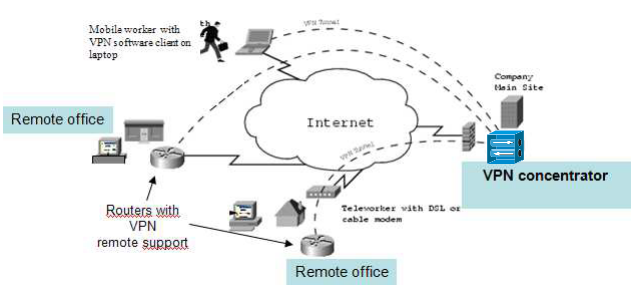
\includegraphics[scale=0.8]{figures/ex/VPN.png}
\caption{VPN IPSec}
\end{figure}
\end{center}

Risoluzione:

$S=0.01$. VPN IPSec. Accesso da remoto ad Internet e si basa sulla presenza di un \textit{VPN Concentrator} (concentratore di reti virtuali). IPSec, SSL. Meccanismi di sicurezza. Concentratore tramite VPN. Un router normale ne supporta fino ad una centinaia di VPN (Grandi aziende come CISCO, IBM). Le richieste di instaurazione arrivano secondo un processo di POISSON. $\lambda = 200\ req/h$. Inoltre $\frac{1}{\mu} = 30\ min$ (tempo medio di servizio). $m=?\ |\ \Pr\{LOSS\} < (S = 0.01)$.

M/M/m/0. Il processo degli arrivi di POISSON. Ci viene chiesto il numero di VPN contemporanee da supportare. Sistema con PERDITA (LOSS). ed ipotesi standard sui vari tempi. $m$ router. $m$ numero di VPN contemporanee. FCFS come disciplina di coda. Non c'è una coda però, quindi non conta tanto. $(\iff d=0, (e=+\infty))$.

Vogliamo utilizzare le tabelle (B di ERLANG). Il \underline{CARICO MEDIO di LAVORO} (INTENSIT\`A DI TRAFFICO) è $(\frac{\lambda}{\mu}) = (200 x 0.5) = 100 \implies (118=m)$. $S = 0.1$ (percentuale di perdita). [ERLANG] Sebbene sia in realtà una quantità adimensionata.

\newpage

\subsection{Sistemi a coda M/M/inf}

Sistema a coda costituito da un insieme illimitato di router. NON ABBIAMO FILA DI ATTESA! (Risorse illimitate). I clienti NON sono costretti a permanere in fila di attesa. Essa è quindi praticamente irrilevante. $N(t)$ al solito è il numero di clienti nel sistema a tempo $t$. Spazio degli stati di dimensione illimitata $\iff S=\{0,1,2,\ \dots\}$. Stesse ipotesi. $N(t)$  CATENA DI MARKOV a tempo continuo (CMTC), nascita e morte, con il seguente DTT:

\begin{center}
\begin{tikzpicture}[->, >=stealth', auto, semithick, node distance=2.3cm]
\tikzstyle{every state}=[fill=white,draw=black,thick,text=black,scale=0.8]
\node[state]    (0)                     {$0$};
\node[state]    (1)[right of=0]   {$1$};
\node[state]    (2)[right of=1]   {$2$};
\node[state] (d) [right of=2] {\ldots};
\node[state]    (im1)[right of=d]   {$i-1$};
\node[state]    (i)[right of=im1]   {$i$};
\node[state]    (ip1)[right of=i]   {$i+1$};
\node[state]    (ip2)[right of=ip1]  {$i+2$};
\node[state]    (d2)[right of=ip2]   {\ldots};
\path
(0) edge[bend left]     node{$\lambda$}         (1)
(1) edge[bend left]     node{$\lambda$}         (2)
    edge[bend left,below]    node{$\mu$}            (0)
(2) edge[bend left]     node{$\lambda$}           (d)
    edge[bend left,below]    node{$2\mu$}             (1)
(d) edge[bend left]         node{$\lambda$}   (im1)
	edge[bend left,below]   node{$3\mu$}          (2)
(im1) edge[bend left]       node{$\lambda$}  (i)
	  edge[bend left,below]   node{$(i-1)\mu$}     (d)
(i)   edge[bend left]   node{$\lambda$}      (ip1)
      edge[bend left,below]  node{$i\mu$}          (im1)
(ip1) edge[bend left]       node{$\lambda$}  (ip2)
	 edge[bend left,below]   node{$(i+1)\mu$}      (i)
(ip2)edge[bend left]       node{$\lambda$}  (d2)
	 edge[bend left,below]   node{$(i+2)\mu$}     (ip1)
(d2)edge[bend left,below]    node{$(i+3)\mu$}     (ip2);
\end{tikzpicture}
\end{center}

Abbiamo:

\[
	\left\{
	\begin{aligned}
	&\lambda_i=\lambda,\ i\geq 0\\
	&\mu_i=i\mu,\ i\geq 1
	\end{aligned}
	\right.
\]

Tassi di nascita $\lambda$, tassi di morte $i\mu$. Numero di stati illimitato. La CATENA è OMOGENEA, IRRIDUCIBILE. Dobbiamo vedere se è ERGODICA:

\[
	\left\{
	\begin{aligned}
	&[\pi_i = \pi_0 (\frac{\lambda}{\mu})^i \frac{1}{i!}]\\
	&[\pi_0 = \frac{1}{1+\sum_{k=1}^\infty{(\frac{\lambda}{\mu})^k \frac{1}{k!}}}]
	\end{aligned}
	\right.
\]

Anzitutto come sempre inglobiamo il termine 1 nella sommatoria dell'ultima equazione. Essa converge sempre. Abbiamo:

\[
	\pi_0 = \frac{1}{\sum_{k=0}^\infty{(\frac{\lambda}{\mu})^k \frac{1}{k!}}} = \e^{-\frac{\lambda}{\mu}}
\]

ove si è sfruttato il fatto che: $[\sum_{i=0}^\infty{x^i\frac{1}{i!}} = \e^x]$. Quindi NO CONDIZIONE DI ERGODICIT\`A. Tale serie CONVERGE SEMPRE. Converge sempre a patto che $\{\lambda,\mu\}$ siano finiti $(\iff \lambda,\mu <+\infty)$. Abbiamo:

\[
	\pi_i = \pi_0 (\frac{\lambda}{\mu})^i \frac{1}{i!} = (\frac{\lambda}{\mu})^i \frac{1}{i!}\e^{-\frac{\lambda}{\mu}},\ i\geq 0
\]

\underline{CATENA SEMPRE ERGODICA}. Non dobbiamo soddisfare nulla. Notiamo subito che riflette una DISTRIBUZIONE DI POISSON di parametro $\frac{\lambda}{\mu}$. Quindi: $[\bar{N} = (\frac{\lambda}{\mu})]$, anche se l'avrei potuto pure trovare con Little questo risultato: $\bar{N} = \lambda (\frac{1}{\mu})$. Quanto abbiamo detto vale per tempi di servizio distribuiti genericamente (\underline{\underline{M/G/$\infty$}}).
Tale sistema a coda è utilizzato per la modellazione dei tempi di propagazione. I tempi di propagazione sono considerati all'incirca costanti e pari a circa $(\sim \frac{2}{3} c)$.

%************************************************
% Chapter 3: AFFIDABILITA' E DISPONIBILITA'
%************************************************
% !TEX encoding = UTF-8
% !TEX TS-program = pdflatex
% !TEX root = ../nt.tex
% !TEX spellcheck = it-IT

%************************************************
\chapter{Affidabilità e Disponibilità}
\label{cap:relavl}
%************************************************\\

\section{Starting Point}

\subsection{Exercise}

CSP = \textit{Content Service Provider}. Abbiamo una batteria di $K$ server, tutti equivalenti. Server soggetti a guasti. $M$ server di backup. Quando un server si blocca viene sostituito con un server di backup, SE DISPONIBILE. Se i $K$ server funzionano tutti siamo in "\textit{Normal State}", Se inferiori a $K$ il sistema si blocca e siamo in "\textit{Failure State}". Ce ne devono essere almeno $K$.

\{TTF per il processo expneg. con parametro $f_p$, TTF memoria expneg. con parametro $f_m$, TTF disco expneg. con parametro $f_d$\}.

DTT, probabilità di regime, frazione di tempo Failure State, MTTF del sistema; durata media dell'intervallo di tempo tra un istante in cui il servizio è attivato e l'istante successivo corrispondente alla sospensione del servizio.

In totale ci sono $\underline{K+M}$ server (server attivi + server di backup). La situazione normale sarebbe il seguente tableau: $\{K,0,M\}$, ove i tre parametri indicano rispettivamente i server funzionanti della server farm, quelli in riparazione e quelli di backup. Ad un certo punto potrebbe accadere che nella server farm vi siano $K$ server ed $M$ in riparazione. Un ulteriore guasto della server farm porterebbe il sistema ad entrare in Failure State. Dinamica relativa al sistema. Definizione di Stato: processo stocastico: numero di server nella server farm e nei server di backup. Questa definizione di stato ci va bene per un processo Markoviano. Le tre v.a. sono indipendenti. Il tempo di guasto di un server sarà il minimo di queste tre v.a. dei TTF. Se quindi $f=f_p+f_m+f_d$, allora il tempo di guasto del server sarà tale che $TTF \sim EXP(f)$. I tempi di guasto dei vari server sono v.a. indipendenti. Le riparazioni procedono in parallelo tra di loro. Tempi di riparazione indipendenti dai tempi di guasto $\iff$ PROCESSO MARKOVIANO, il cui DTT è il seguente:

\begin{center}
\begin{tikzpicture}[->, >=stealth', auto, semithick, node distance=2cm]
\tikzstyle{every state}=[fill=white,draw=black,thick,text=black,scale=1]
\node[state]    (KPM)                     {$K+M$};
\node[state]    (KPMM1)[right of=KPM]   {$K+M-1$};
\node[state]    (KPMM2)[right of=KPMM1]   {$K+M-2$};
\node[state] (KPMM3) [right of=KPMM2] {$K+M-3$};
\node[state]    (d)[right of=KPMM3]   {\ldots};
\node[state]    (KP1)[right of=d]   {$K+1$};
\node[state]    (K)[right of=KP1]   {$K$};
\node[state]    (KM1)[right of=K]  {$K-1$};
\path
(KPM) edge[bend left]     node{$Kf$}         (KPMM1)
(KPMM1) edge[bend left]     node{$Kf$}         (KPMM2)
    edge[bend left,below]    node{$\mu$}            (KPM)
(KPMM2) edge[bend left]     node{$Kf$}           (KPMM3)
    edge[bend left,below]    node{$2\mu$}             (KPMM1)
(KPMM3) edge[bend left]         node{$Kf$}   (d)
	edge[bend left,below]   node{$3\mu$}          (KPMM2)
(d) edge[bend left]       node{$Kf$}  (KP1)
	  edge[bend left,below]   node{$4\mu$}     (KPMM3)
(KP1)   edge[bend left]   node{$Kf$}      (K)
      edge[bend left,below]  node{$(M-1)\mu$}          (d)
(K) edge[bend left]       node{$Kf$}  (KM1)
	 edge[bend left,below]   node{$M\mu$}      (KP1)
(KM1) edge[bend left,below]   node{$(M+1)\mu$}     (K);
\end{tikzpicture}
\end{center}

Il numero di stati è finito $(\iff \cardinality{stati}<+\infty)$. Si suppone che le riparazioni avvengano in parallelo, altrimenti se ci fosse una Single Repair Facility $\mu$ sarebbe costante. Quindi abbiamo: $N(t)=K+M$, ovvero $K$ server nella server farm che si possono guastare. Il tempo di guasto è dato da $\rightarrow$

\[
	\phi_{K+M}(t) = \underline{\min{(\dots)}}
\]

ove la parte sottolineata indica i tempi di guasto residui al tempo $t$. Se siamo nello stato $K$, vi sono $M$ \underline{in riparazione} e 0 nella stanza dei server di backup. Può accadere che ad un certo punto si guasti un ulteriore server della server farm $\implies$ FAILURE STATE. La velocità totale di uscita dallo stato $K+M$ sarebbe proprio $Kf$.

\begin{itemize}

\item{\textbf{NORMAL STATE}} fino a $K$;
\item{\textbf{FAILURE STATE}} $K-1$;
\end{itemize}

Oscillazione tra normal state e failure state. La seguente Catena di Markov vagherà tra questi stati. Non esiste una singola definizione di stato. Ce ne possono essere differenti. Alcune volte delle differenti definizioni di stato potrebbero portare allo stesso DTT. Considerando ad esempio $N(t)$ come il numero di server in riparazione avremo il seguente DTT:

\begin{center}
\begin{tikzpicture}[->, >=stealth', auto, semithick, node distance=2cm]
\tikzstyle{every state}=[fill=white,draw=black,thick,text=black,scale=1]
\node[state]    (0)                     {$0$};
\node[state]    (1)[right of=0]   {$1$};
\node[state]    (2)[right of=1]   {$2$};
\node[state] (3) [right of=2] {$3$};
\node[state]    (d)[right of=3]   {\ldots};
\node[state]    (MM1)[right of=d]   {$M-1$};
\node[state]    (M)[right of=MM1]   {$M$};
\node[state]    (MP1)[right of=M]  {$M+1$};
\path
(0) edge[bend left]     node{$Kf$}         (1)
(1) edge[bend left]     node{$Kf$}         (2)
    edge[bend left,below]    node{$\mu$}            (0)
(2) edge[bend left]     node{$Kf$}           (3)
    edge[bend left,below]    node{$2\mu$}             (1)
(3) edge[bend left]         node{$Kf$}   (d)
	edge[bend left,below]   node{$3\mu$}          (2)
(d) edge[bend left]       node{$Kf$}  (MM1)
	  edge[bend left,below]   node{$4\mu$}     (3)
(MM1)   edge[bend left]   node{$Kf$}      (M)
      edge[bend left,below]  node{$(M-1)\mu$}          (d)
(M) edge[bend left]       node{$Kf$}  (MP1)
	 edge[bend left,below]   node{$M\mu$}      (MM1)
(MP1) edge[bend left,below]   node{$(M+1)\mu$}     (M);
\end{tikzpicture}
\end{center}


ove cambierebbero solo le label rispetto al precedente.
Non è importante il modo in cui si chiamino gli stati, ma le loro transizioni! PROCESSO STOCASTICO: numero di server in riparazione al tempo $t$; CATENA ERGODICA (OMOGENEA, IRRIDUCIBILE con $\cardinality{stati}<+\infty$). In funzione della distribuzione di regime dobbiamo trovare altre quantità:

$\pi_{M+1}$ sarebbe la frazione di tempo a regime ove il servizio è sospeso, quindi $\underline{1-\pi_{M+1}} = \underline{\pi_0+\ \dots+\ \pi_M}$ sarebbe invece la frazione di tempo a regime nel quale il sistema si trova nello stato NORMAL, per via della condizione di NORMALIZZAZIONE. Il LHS è proprio la DISPONIBILIT\`A.

$\underline{1-\pi_{M+1}}$ AVAILABILITY del mio sistema di servizio. MTTF: durata (media) dell'intervallo che è costituito dall'istante di tempo di funzionamento alla sospensione. MTTF = \textit{Mean Time To Failure}. Rappresenta un processo stocastico, sebbene non markoviano, con stati: $S=\{ON,\ OFF\}$, ove ON sta per NORMAL ed OFF per FAILURE. Ad un certo punto la catena sarà in $M$. L'MTTF è la durata media dell'intervallo di tempo che va dall'inizio dello stato $M$ sino all'istante di Failure, ovvero un istante immediatamente prima delle sospensione del servizio. Invece MTTR significa \textit{Mean Time To Recovery}.

\begin{defn}{\textbf{AVAILABILITY}}

L'AVAILABILITY è la frazione del tempo in cui il sistema sta ad erogare il servizio:

\[	
	A := [\frac{MTTF}{MTTF+MTTR}]
\]

\end{defn}

Noi parleremo di ALTA DISPONIBILIT\`A. 5-9 ($99.999\%$), che rappresenta un downtime annuo di circa 5 minuti. Disponibilità molto alta in realtà bancarie. L'MTTR corrisponde al tempo medio di soggiorno della mia catena nello stato $M+1$. Il valor medio del tempo di soggiorno è $\frac{1}{(M+1)\mu}$. 

Consideriamo il seguente risultato:

\[
	MTTF = \frac{1}{(M+1)\mu\pi_{M+1}} - (\dots)
\]

dove $(\dots)$ rappresenta il tempo medio di soggiorno da sottrarre (durata media di quell'intervallo). Quindi:

\[
	MTTF = (\dots) = \frac{1}{(M+1)\mu\pi_{M+1}} - \frac{1}{(M+1)\mu} = \frac{1}{(M+1)\mu} \frac{1-\pi_{M+1}}{\pi_{M+1}} \implies
\]
\[
	\implies [\frac{MTTF}{\frac{1}{(M+1)\mu}} = \frac{1-\pi_{M+1}}{\pi_{M+1}}] \implies \frac{MTTF}{MTTR} = \frac{1-\pi_{M+1}}{\pi_{M+1}}
\]

Vale il BILANCIAMENTO LOCALE. Abbiamo che:

\begin{itemize}

\item{$\frac{1}{(M+1)\mu}$} è il tempo medio di soggiorno della mia catena nello stato $M+1$;
\item{$\frac{1}{(M+1)\mu\pi_{M+1}}$} è il tempo medio di ricorrenza (o di ritorno) nello stato $M+1$;
\end{itemize}

La differenza ci ritorna l'MTTF. Abbiamo sfruttato il fatto che la frequenza dell'evento ritorno nello stato di normal state è: $\pi_{M+1}(M+1)\mu$, mentre a titolo informativo la frequenza dell'evento ingresso nello stato di failure è $\pi_MKf$. Le due frequenze sono ovviamente uguali in virtù dell'applicazione dell'equazione di bilanciamento locale, dato che questa CMTC è di tipo Nascita e Morte.

Se si volesse utilizzare la tecnica degli stati assorbenti (vedasi \textbf{CMTC with Absorbing States}), allora bisognerebbe considerare come STATO ASSORBENTE \{M+1\}, e bisognerebbe tenere opportunamente in conto le condizioni iniziali del processo.

Sistemi di servizio che possono trovarsi in due stati: \{NORMAL STATE, FAILURE STATE\}, mappati rispettivamente in $SYS:\ \{ON,\ OFF\}$. Prendiamo in considerazione due sistemi:

\begin{itemize}

\item{\textit{Primo sistema}}: \newline
Tale sistema mediamente per $1s$ si trovi nello stato OFF, e per $9s$ nello stato ON. La disponibilità di questo sistema è: $A = \frac{9s}{10s} = 90\%$, ovvero per il $90\%$ del tempo il sistema è perfettamente funzionante, nello stato di ON.

\item{\textit{Secondo sistema}}: \newline
Tale sistema invece è UP per $0.9s$, e down per $0.1s$. Abbiamo sempre una disponibilità di $A = \frac{0.9s}{1s} = 90\%$, come il primo sistema;

\end{itemize}

La \underline{\underline{disponibilità}} è la medesima per i due sistemi, ma l'affidabilità invece è maggiore nel primo (non ha a che fare con il tempo di Recovery).


\begin{defn}{\textbf{AFFIDABILIT\`A}}

L'Affidabilità è formalmente definita come:

\[
	R(t) := \Pr\{X > t\} = Reliability(t)
\]
\end{defn}

Non sarebbe nient'altro che la CDF complementare della v.a. $X$, la quale rappresenta il tempo di vita del sistema. Non pensiamo alla riparazione o sostituzione. Si parte dall'affidabilità dei singoli componenti. Per l'analisi di affidabilità sono molto utili gli RBD, ovvero i \textit{Reliability Block Diagram}.

\subsection{Ridondanza}

Web server SW processo applicativo che si guasta con un failure rate $\gamma_p$. In esecuzione con una macchina che si guasta indipendentemente a failure rate $\gamma_m$. Il failure rate corrisponde ad un parametro della distribuzione esponenziale. Definizione di failure rate dipendente dal tempo. Vi è un meccanismo automatico di \textit{Failure Detection}, basato sul polling. Il tempo medio necessario per rilevare il failure sul server sia $\frac{1}{\delta_p}$ e che $\frac{1}{\delta_m}$ sia il tempo medio di rilevazione failure macchina.

Quando la macchina ha un malfunzionamento, il processo applicativo è migrato su una macchina di riserva, se \underline{DISPONIBILE}. $\frac{1}{\tau_m}$ è il tempo medio necessario per avviare la macchina di backup. Se invece si ha un guasto soltanto del processo server, viene automaticamente riavviato sulla stessa macchina. Il tempo medio di restart del server software è $\frac{1}{\tau_p}$. Tipicamente $[\tau_p > \tau_m] \implies \frac{1}{\tau_p} < \frac{1}{\tau_m}$. C'è una piccola probabilità $(1-c)$ che il restart del processo sulla stessa macchina non vada a buon fine, nel qual caso è avviato sulla macchina di riserva. Questo schema di (re)start automatico dopo i guasti è anche chiamato "\textit{cold replication}". Quando una macchina crasha, è necessario un recovery più complesso dal relativo rate $\mu$. Il Web server è considerato disponibile quando sia il processo server che la macchina sulla quale esso gira sono entrambi funzionanti. Si valuti la \textit{Steady-State Availability} del server, assumendo che non vi siano ulteriori guasti del processo o della macchina fino a che non siano stati adeguatamente trattati (risolti).

Quindi la DISPONIBILIT\`A viene meno quando nè il processo nè la macchina sono funzionanti. AFFIDABILIT\`A di un sistema cold-replicated $\implies$ RIDONDANZA. RIDONDANZA o \textit{REPLICATION ATTIVA} quando vi sono oltre ai server operativi anche dei server di backup, tutti quanti soggetti alla stessa quantità di lavoro (in tal caso anche quelli di backup lavorano come quelli normali). Si suppone che il failure rate sia il medesimo per entrambi i tipi. Il contrario è la REPLICATION PASSIVA $\rightarrow$ \{WARM REPLICATION, COLD REPLICATION\}. Si immagini di avere due server, due macchine. Uno attivo è l'altro di backup. Con la WARM, di tanto in tanto quello di backup interagisce con quello attivo per ricevere le sue strutture dati. Un malfunzionamento di quello attivo fa sì che si attivi quello di backup. Ma il relativo tempo del recovery è molto basso. Ci piace questo, però a trasferire queste strutture dati periodicamente, una parte delle capacità elaborative sarà riservata a questa mansione. Potrebbe invece eseguire altri jobs al posto di questi. Vantaggi in tempi di Recovery, però il problema è legato ad un throughput più basso del server attivo. Con quella a freddo abbiamo un tempo di recovery più alto, ma sull'attivo sfruttiamo perlomeno tutta la capacità elaborativa. Parametri: \{performance, affidabilità della rete (dei vari dispositivi di cui la rete si compone)\ (\textit{reliability R(t), fault tolerance}), Sicurezza dati\}. L'esercizio in questione propone la ridondanza di un Server. Potrebbero esserci dei \textit{WATCH-DOG}, ovvero dei "cani da guardia" che controllano il server primario. Controllo delle eventuali degradazioni delle prestazioni in un cluster - Policing, disciplina decidibile.

Studiamo il sistema con un approccio Markoviano. DTT della CMTC che modella il sistema. Faremo l'ipotesi di distribuzione esponenziale per le v.a. in gioco (Anche per la distribuzione relativa al Failure Detection Time).

\[
	\left\{
	\begin{aligned}
	&F_p \sim EXP(\gamma_p),\ F_m \sim EXP(\gamma_m)\\
	&D_p \sim EXP(\delta_p),\ D_m \sim EXP(\delta_m) \\
	&R_p \sim EXP(\tau_p),\ R_m \sim EXP(\tau_m)
	\end{aligned}
	\right.
\]

Rispettivamente, le prime due equazioni della prima riga indicano la distribuzione dei time to failure di un processo o della macchina, le successive due della seconda riga indicano la distribuzione dei time to failure detection del processo o della macchina, e le ultime due della terza riga indicano la distribuzione del time to (re)start del processo \underline{sulla stessa macchina} (SAME MACHINE) o del riavvio del processo sulla macchina di riserva (SPARE MACHINE). $(1-c)$ rappresenta invece la probabilità che il riavvio del processo sulla stessa macchina fallisca. Quindi $c$ è il \textit{coverage factor}, ovvero la probabilità di successo del riavvio del processo. Infine abbiamo: $C_r \sim EXP(\mu)$, ovvero il tempo di riparazione per una macchina andata in crash (crashed machine recovery). Il DTT è il seguente:

\begin{center}
\begin{tikzpicture}[->, >=stealth', auto, semithick, node distance=3cm]
\tikzstyle{every state}=[fill=white,draw=black,thick,text=black,scale=1]
\node[state]    (01X1)                     {$01X1$};
\node[state]    (11X1)[above right of=01X1]   {$11X1$};
\node[state] (0D1X1) [right of=01X1] {$0D1X1$};
\node[state]    (X0DX1)[below of=01X1]   {$X0DX1$};
\node[state]    (11X0D)[right of=11X1]   {$11X0D$};
\node[state]    (11X0)[below of=11X0D]   {$11X0$};
\node[state]    (0D1X0)[right of=11X0D]   {$0D1X0$};
\node[state]    (01X0)[right of=0D1X0]  {$01X0$};
\node[state]    (F)[below of=01X0]  {$F$};
\node[state]    (X0X1)[below left of=F]  {$X0X1$};
\path
(11X1) edge[bend left]     node{$\gamma_m$}         (11X0D)
       edge[right]   node{$\gamma_m$}   (X0DX1)
       edge[bend left,above]     node{$\gamma_p$}   (0D1X1)
(01X1) edge[bend left]     node{$c\tau_p$}         (11X1)
    edge[bend right]    node{$tau_p(1-c)$}            (X0X1)
(0D1X1) edge[bend right,above left]     node{$\delta_p$}           (01X1)
(X0DX1) edge[bend right]         node{$\delta_m$}   (X0X1)
(X0X1) edge[bend left,right]        node{$\tau_m$} (11X0)
(11X0D) edge[bend left]       node{$\delta_m$}  (11X0)
(0D1X0)   edge[bend left]   node{$\delta_p$}      (01X0)
(01X0) edge[bend left]       node{$c\tau_p$}  (11X0)
	 edge[bend left]   node{$c(1-\tau_p)$}      (F)
(F) edge[bend left]   node{$\mu$}     (X0X1)
(11X0) edge[bend right] node{$\gamma_p$} (0D1X0)
 edge[bend right] node{$\gamma_m$} (F)
 edge[bend right] node{$\mu$} (11X1);
\end{tikzpicture}
\end{center}

La definizione di stato si basa sui seguenti stati degli elementi \{(Processo primario, Macchina primaria), (Processo secondario, Macchina secondaria)\}, riassumibili nel seguente apposito tableau:

\[
	\begin{bmatrix}
	P_p&P_m\\S_p&S_m
	\end{bmatrix}
\]

Tale è la rappresentazione del DTT di una CMTC che modella un Web Server con Cold Replication con una macchina di backup. $\{P_p,\ P_m\}$ rappresentano rispettivamente gli stati del processo primario e della macchina primaria sulla quale questo processo è in esecuzione. I pedici $\{p,m\}$ si riferiscono rispettivamente al processo od alla macchina. Gli altri due indici, $\{S_p,\ S_m\}$ stanno per SPARE o secondary. E stanno per lo stato del processo server di backup e della relativa macchina sulla quale esso sta in esecuzione, al solito. $P \rightarrow primary,\ S \rightarrow spare$. $"1" \rightarrow$ processo/macchina up; $"0" \rightarrow"$ processo/macchina down. Se $P_p=1\ \lor P_m=1 \implies$ il processo/macchina primario/a è up. $P_p=0\ \lor\ P_m=0 \implies$ processo/macchina primaria down. Vale anche per gli altri ovviamente. $"0D" \rightarrow$ processo/macchina è failed (guasta), con malfunzionamento, ma il rispettivo guasto non è ancora stato rilevato (To be detected). $"X" \rightarrow$ don't care. Valori possibili. Possiamo pensare di partire dallo stato: \{1,1,X,1\} $\implies P_p=P_m=1$. (processo e macchina primaria entrambi UP). Macchina secondaria funzionante e non ci interessa del processo secondario. Ai fini delle transizioni di stato, ci può essere un malfunzionamento o del processo primario, o della macchina primaria od ancora quella di backup. $\gamma_p$ è il parametro della distribuzione esponenziale che modella il TTF del processo. Supponiamo si sia verificato un malfunzionamento del processo primario. Macchina primaria/secondaria entrambe UP $\rightarrow 0D=P_p \rightarrow P_p=0$. Altra transizione. Macchine ancora entrambe UP. Dopo che il sistema di Failure Detection avrà fatto per l'appunto detection del failure, a velocità $\delta_p$, lo stato sarà: \{0,1,X,1\}. A questo punto si tenta di riavviare il processo (come accade tipicamente nei SO) sulla stessa macchina. Abbiamo un Coverage Factor pari a $c$, ovvero pari alla probabilità che il riavvio vada a buon fine. $(1-c)$ è per contro, la probabilità che vada male il riavvio. Se il riavvio sulla stessa macchina ha successo, migriamo conseguentemente verso lo stato iniziale \{1,1,X,1\} a velocità $c\tau_p$. Altrimenti con velocità $(1-c)\tau_p$ migriamo verso lo stato \{X,0,X,1\}. Siamo in situazione di macchina primaria Down. Con certezza la macchina per me è in crash. Macchina inutilizzabile. Siamo quindi in \{X,0,X,1\}. Macchina 1 in crash. Bisogna quindi cambiare macchina. $\tau_p$ è il parametro che caratterizza la distribuzione esponenziale relativa al restart time della macchina stessa. Consideriamo la v.a. tempo di soggiorno residuo nello stato: \{0,1,X,1\}, di indice 4. $\phi_4 \sim EXP(\mathord{\cdot})$. Consideriamo:

\[
	\Pr\{\phi_4(t) > \tau\} = \Pr\{R_{Rp} > \tau\} = \e^{-\tau_p\tau}
\]

dove $R_{Rp}$ rappresenta il restart time del processo (residuo), e tale è la probabilità che esso sia maggiore di $\tau$. Indica quanto manca ancora affinché il restart finisca. $R_{Rp}$ sarà distribuita proprio come il Restart Time del processo sulla macchina attiva. $R_p$ è il restart time, mentre $R_{Rp}$ è il restart time residuo. Nell'istante $t$ stiamo quindi in questo stato. Questo restart potrebbe andar bene od andar male. Velocità totale di uscita banalmente $\tau_p$. Quindi:

\[
	\tau_{i,j} = \frac{q_{i,j}}{-q_{ii}} = \tau_{4,1} = \frac{q_{4,1}}{-q_{4,4}} = \frac{q_{4,1}}{\tau_p} \implies
\]
\[
	\implies \tau_{4,1} = c \implies q_{4,1}=c\tau_p
\]

La macchina è andata in crash, a questo punto. Bisogna quindi cambiare macchina. Ci vuole un altro tempo che indichiamo con $R_m$, ovvero il restart time del processo sulla macchina secondaria. Con velocità $\tau_m$ arriveremo da \{X,0,X,1\} $\rightarrow$ \{1,1,X,0\} (Non ho più una macchina di riserva). Quella primaria si è sostanzialmente scambiata con la secondaria (funzionante). A velocità $\mu$ dopodiché, avremo la riparazione e migriamo verso lo stato iniziale, nuovamente: \{1,1,X,1\}. Possono accadere però altre cose. Dobbiamo anche considerare che, o accada un malfunzionamento della macchina primaria o della secondaria. \{1,1,X,1\} $\rightarrow$ \{X,0D,X,1\} $\rightarrow$ \{X,0,X,1\} a velocità $\delta_m$, quest'ultimo passaggio. Poi arriveremo verso \{1,1,X,0\} ad avvenuta sostituzione. $\gamma_m$ è il parametro che caratterizza la distribuzione esponenziale della $F_m$, ovvero il TTF della macchina. Sempre $\gamma_m$ per la failure. Partiamo da \{1,1,X,0\}. NO macchina secondaria a disposizione. O malfunzionamento del processo primario o della macchina secondaria. Se accade un malfunzionamento del processo primario, migrerò con velocità $\gamma_p$ verso \{0D,1,X,0\}, ed a velocità $\delta_p$ verso \{0,1,X,0\}. Se si verifica un failure della macchina andremo in FAILURE direttamente a velocità $(1-c)\tau_p$. Ma se a partire da \{1,1,X,0\} si guasta completamente la macchina, allora migreremo direttamente in \textbf{FAILURE} totale a velocità $\gamma_m$. Notiamo che siamo in situazione di SRF (\textit{Single Repair Facility}).

Studio di fattibilità. Non è importante l'etichetta che attribuiamo agli stati quanto il loro significato. A questo punto li etichettiamo. Procedura di Labelizing. Distribuzioni di regime. Sistema di 10 equazioni (9 eq. + 1 eq. normalizzazione). Sfruttiamo la conoscenza del valore dei diversi parametri in gioco.
Si valuti quindi la Steady-State Availability del Server. Stati nei quali il Web Server funziona. Gli stati dove $P_p=1$ sono:

\[
	\left\{ \begin{bmatrix}1&1\\X&1\end{bmatrix},\ \begin{bmatrix}1&1\\X&0\end{bmatrix},\ \begin{bmatrix}1&1\\X&0D\end{bmatrix} \right\}
\]

A questo punto, abbiamo che: $[A = \pi_1 + \pi_6 + \pi_7]$, secondo la nuova notazione indiciale rappresentata nella seguente maniera, nella notazione \textit{State name} $\rightarrow$ \textit{State index}:

\begin{itemize}
\item{\{1,1,X,1\}} $\rightarrow$ 1;
\item{\{0D,1,X,1\}} $\rightarrow$ 2;
\item{\{X,0D,X,1\}} $\rightarrow$ 3;
\item{\{0,1,X,1\}} $\rightarrow$ 4;
\item{\{X,0,X,1\}} $\rightarrow$ 5;
\item{\{1,1,X,0D\}} $\rightarrow$ 6;
\item{\{1,1,X,0\}} $\rightarrow$ 7;
\item{\{0D,1,X,0\}} $\rightarrow$ 8;
\item{\{0,1,X,0\}} $\rightarrow$ 9
\item{\{1,1,X,1\}} $\rightarrow$ 10;

\end{itemize}

\[
	\left\{
	\begin{aligned}
	&\frac{1}{\gamma_p} = 10\ days, \frac{1}{\gamma_m} = 20\ days\\
	&\frac{1}{\delta_p} = 1 s, \frac{1}{\delta_m} = 0.4/0.5 s\\
	&\frac{1}{\tau_m} = 2\ min, \frac{1}{\tau_p} = 30s
	\end{aligned}
	\right.
\]

\[
	\left\{
	\begin{aligned}
	&\pi_1 = \frac{1}{E},\ \pi_2 = \frac{1}{E} \frac{\gamma_p}{\delta_p},\ \pi_3 = \frac{1}{E} \frac{\gamma_m}{\delta_m},\ \pi_4 = \frac{1}{E} \frac{\gamma_p}{\tau_p}\\
	&\pi_5 = \frac{1}{E} \frac{[\gamma_m + (1-c)\tau_p][\mu + 2\gamma_m + (1-c)\tau_p]}{\mu\tau_m}\\
	&\pi_6 = \frac{1}{E} \frac{\gamma_m}{\delta_m},\ \pi_7 = \frac{1}{E} \frac{2\gamma_m + (1-c)\gamma_p}{\mu}\\
	&\pi_8 = \frac{1}{E} [2\gamma_m + (1-c)\gamma_p]\gamma_p,\ \pi_9 = \frac{1}{E} \frac{[2\gamma_m + (1-c)\gamma_p]\gamma_p}{\mu\tau_p}\\
	&\pi_{10} = \frac{1}{E} \frac{[2\gamma_m + (1-c)\gamma_p][\gamma_m + (1-c)\gamma_p]}{\mu^2}
	\end{aligned}
	\right.
\]

dove:

\[
	E = 1 + \frac{\gamma_p}{\delta_p} + 2\frac{\gamma_m}{\delta_m} + \frac{\gamma_p}{\delta_p} + \frac{[\gamma_m + (1-c)\gamma_p][\mu+2\gamma_m + (1-c)\gamma_p]}{\mu\tau_m} +
\]
\[
	+ \frac{2\gamma_m + (1-c)\gamma_p}{\mu} [1+\frac{\gamma_p}{\delta_p} + \frac{\gamma_p}{\tau_p}] + \frac{[2\gamma_m + (1-c)\gamma_p][\gamma_m + (1-c)\gamma_p]}{\mu^2}
\]

ed otteniamo alla fine:

\[
	A = \pi_1 + \pi_6 + \pi_7 = \frac{1}{E} [1+\frac{\gamma_p}{\delta_p} + \frac{2\gamma_m + (1-c)\gamma_p}{\mu}]
\]

Abbiamo così trovato la Steady-State Availability $A$.

\section{Affidabilità}

\{\underline{Affidabilità}, \underline{Disponibilità}\}. Come può esser valutata l'Affidabilità di un Sistema. Affidabilità di un Dispositivo / servizio di Rete. Concetti legati ma differenti.

Reliability $R(t)$. Affidabilità. Indipendentemente dalla rete / servizi di rete. L'Affidabilità può esser applicata dappertutto. L'Affidabilità va PROGETTATA. \underline{Reliability Engineering}. Di mezzo ci sono queste tecniche, che si servono principalmente dei \newline \underline{diagrammi a blocchi dell'affidabilità}, detti RBD. Utilizzo delle CATENE DI MARKOV. Dato $\mathit{S}$ un sistema, componente, apparato, switch lvl 2 o lvl 3, l'affidabilità esprime la capacità, relativamente a quel sistema, di funzionare correttamente per un certo periodo di tempo. $X$ è il time to failure del sistema (lifetime del sistema). Indichiamo con $f(t)$ la PDF di $X$, ovvero la densità di probabilità. Sia invece $F(t)$ la CDF di $X$ (funzione di distribuzione cumulativa). L'Affidabilità $R(t)$ è definita come:

\begin{defn}{\textbf{Affidabilità}}

\[
	R(t) := \Pr\{X > t\} = 1-F(t) = F^c(t)
\]

\end{defn}

Non è nient'altro che la CDF complementare, ed indica la probabilità che il TTF sia maggiore di un certo tempo $t$, non meglio definito per il momento
Probabilità che $\mathit{S}$ sia funzionante correttamente in $[0,t)$. $\Pr\{\mathit{S}\ correctly\ working\ in\ [0,t)\}$. Tempo di vita almeno pari a $t$, ovvero che $\mathit{S}$ sopravviva per almeno $t$ unità di tempo. Normalmente si suppone che il sistema lavori correttamente nell'istante iniziale, ovvero $\iff R(0)=1$ (con probabilità unitaria il lifetime sia maggiore di 0). Potrebbe anche accadere che in alcuni casi $\Pr\{X=0\} = p\neq 0$ (che un dispositivo NON funzioni all'inizio). Normalmente si ha invece: $\Pr\{X=0\} = (0=p)$. Tipicamente quindi $R(0)=1$. Poi si suppone che: $[\lim_{t\to+\infty}{R(t)} = 0] \iff$ un sistema NON possa funzionare indefinitamente. Inizialmente funzioni correttamente e prima o poi si guasterà. Sostanzialmente, graficamente parlando, $\Pr\{X > t\}$ rappresenta l'area sottesa dalla relativa PDF $f(t)$ in $[t,+\infty)$. $R(t)$ è la CDF complementare di $X$, quindi vale:

\[
	\left\{
	\begin{aligned}
	&[R(t) = \int_t^{+\infty}{f(x)dx}]\\
	&[R'(t) = -\frac{d F(t)}{dt} = -f(t)]
	\end{aligned}
	\right.
\]

Ovvero che la derivata dell'affidabilità, $R'(t)$, non è nientemeno che la PDF del TTF $X$ o lifetime cambiata di segno. 

Qual'è invece il MTTF? Valor medio del time to failure? (tempo medio di vita):

\[
	MTTF = \E[X] = \int_0^\infty{tf(t)dt} = \int_0^\infty{R(t)dt}
\]

ovvero che il MTTF è sostanzialmente l'integrale dell'affidabilità. Si dimostra integrando per parti.

\[
	\underline{\E[X]} = \int_0^{+\infty}{[1-F(t)]dt} - \int_{-\infty}^0{F(t)dt}
\]

L'integrazione per parti dimostra ciò. Questo vale generalmente quando $\E[X] \leq\geq 0$. Ma se il lifetime è maggiore di 0, come nel nostro caso, dal momento che è una variabile aleatoria soltanto a valori positivi (v.a. positiva), allora banalmente vale che: 

\[
	\int_{-\infty}^0{F(t)dt} = 0 \implies \E[X] = \int_0^{+\infty}{[1-F(t)]dt} = \int_0^\infty{\underline{R(t)}dt}
\]

ovvero che il MTTF è l'integrale dell'affidabilità, come già detto. Ricordiamo che MTTF sarebbe il \textit{Mean Time To Failure}, ed il MTBF significa \textit{Mean Time Between Failure}. Sono sostanzialmente la stessa cosa ma nominate in modo diverso. A volte nei paper della CISCO si preferisce utilizzare il MTBF. I valori possono tranquillamente raggiungere 40 anni. Esistono metodi di calcolo che favoriscono il confronto (Metodi Standard).  

Definiamo il: FAILURE RATE (istantaneo). (Instantaneous) Failure Rate. Partiamo dalla PDF della v.a. $X$ TTF o lifetime:

\[
	f(t) = \frac{d F(t)}{dt} = \lim_{\Delta t\to 0}{[\frac{F(t+\Delta t)-F(t)}{\Delta t}]}
\]

A numeratore abbiamo: $\Pr\{t < X \leq t+\Delta t\}$, per $\Delta t$ sufficientemente piccolo. Per $\Delta t\to 0$, abbiamo che $f(t)\Delta t$ rappresenta la probabilità che il tempo di vita di quella v.a. vari tra $t$ e $t+\Delta t$. Per $\Delta t\to 0$ il prodotto $f(t)\Delta t \to \Pr\{t < X \leq t+\Delta t\}$. Questa è una probabilità NON condizionata. Adesso consideriamo: $\Pr\{t < X \leq t+\Delta t\ |\ X > t\} = (\dots)$, che sarebbe la probabilità che, dato che il sistema è sopravvissuto per $t$ unità di tempo, non sopravviva per ulteriori $\Delta t$ unità di tempo. Abbiamo che:

\[
	(\dots) = \frac{\Pr\{t < X \leq t+\Delta t,\ X > t\}}{\Pr\{X > t\}} = [\frac{\Pr\{t < X \leq t+\Delta t\}}{\Pr\{X > t\}}] \implies
\]

ove si è sfruttato il seguente fatto:

\[
	\{X > t\} \subset \{t < X \leq t+\Delta t\} \implies \Pr\{t < X \leq t\Delta t \cap X > t\} = \Pr\{t < X \leq t+\Delta t\}
\]

A denominatore abbiamo l'Affidabilità $R(t)$. Definiamo ora l'IFT $h(t)$ come:

\begin{defn}{\textbf{(Instantaneous) Failure Rate}}

L'IFT (\textit{Instantaneous Failure Rate}) è definito come:

\[
	h(t) := \lim_{\Delta t \to 0}{[\frac{1}{\Delta t} \frac{\Pr\{t < X \leq t+\Delta t\}}{R(t)}]} = \mathord{\cdot}(t)
\]

\end{defn}

Questa è la definizione del Failure Rate istantaneo. $\Delta t\to 0 \implies h(t)\Delta t$ rappresenta la probabilità che, supponendo che il dispositivo sia sopravvissuto per $t$ unità di tempo, non sopravviva per ulteriori $\Delta t$ unità di tempo. Ma notiamo che:

\[
	h(t) = \lim_{\Delta t\to 0}{\frac{1}{\Delta t} \frac{F(t+\Delta t)-F(t)}{R(t)}} = \frac{f(t)}{R(t)}
\]

ovvero corrisponde al rapporto tra la PDF e la CDF complementare della v.a. $X$. Sappiamo inoltre che: $f(t)=-R'(t) \implies$

\[	
	h(t) = -\frac{(R'(t) = -f(t))}{R(t)} = \frac{-R'(t)}{R(t)}
\]

Ma essendo l'affidabilità una probabilità $\implies R(t) \in [0,1]$. Quindi ne consegue che: $h(t)\geq f(t)$. Ma a questo punto, indipendentemente da $\Delta t\to 0$, abbiamo che: $[h(t)\Delta t\geq f(t)\Delta t]$. Vero indipendentemente dal valore di $\Delta t$. Quindi, ricapitolando, $f(t)\Delta t$ rappresenta la probabilità che il tempo di vita sia compreso tra $t$ e $t+\Delta t$, mentre $h(t)\Delta t$ indica la probabilità che, sapendo che il dispositivo sia sopravvissuto sino a $t$, muoia nei prossimi $\Delta t$. $h(t)$ è quindi sensibilmente più grande di $f(t)$, indipendentemente da $\Delta t$. 

Ci serve un modo teorico per ricavare questi valori. Abbiamo tre macro-fasi di vita del dispositivo, sintetizzabili in un grafico di $h(t)$ in funzione del tempo $t$. Abbiamo un andamento cosiddetto a \textit{CURVA di VASCA DA BAGNO}. Abbiamo la prima fase di mortalità infantile, che include l'avvenimento di eventuali difetti di fabbrica, quindi $h(t)$ è alto. Poi abbiamo la seconda fase, ove $h(t)$ è tipicamente basso, ovvero il ciclo di vita utile del dispositivo. Qualunque malfunzionamento qui deriva da PROBLEMI ESOGENI, ove lo stress è dovuto a cause esterne. Poi abbiamo un'ultima fase di senilità, ove comprensibilmente $h(t)$ torna ad esser nuovamente alto in quanto vi è l'USURA del dispositivo da tener in conto. $h(t)=\frac{f(t)}{R(t)}=\frac{-R'(t)}{R(t)}$ rappresenta quindi la velocità alla quale un sistema tende a rompersi.

Il Failure Rate NON è un qualcosa di costante, ma varia con il tempo! Nel calcolo pratico si ipotizza sempre che siamo nella seconda fase di vita del dispositivo, ovvero quella di vita utile.

I seguenti elementi: $\{MTTF=\E[X],\ R(t),\ h(t)\}$ sono in stretta relazione tra di loro. Sia $N_0$ il numero di dispositivi messi ad operare tutti insieme nell'istante $(t_0=0)$. Siano nelle stesse condizioni di lavoro di partenza. Per tutti INIZIA il tempo di vita. Same working conditions. Al generico istante $t$, possiamo osservare lo stato di questi dispositivi. $N_S(t)$ sia il numero di dispositivi SURVIVED (sopravvissuti), per i quali il tempo di vita NON è terminato. Vale: $N_F(t) = \underline{N_0-N_S(t)} \implies [N_S(t) + N_F(t) = N_0]$ (popolazione iniziale). Se dovessi vedere come varia questa funzione $N_S(t)$ al variare del tempo, avrei una funzione a gradino decrescente. I guasti, ovvero le variazioni del grafico, avvengono in istanti $t_i$. L'intervallo $[0,t_1]$ comprende il tempo di vita del primo dispositivo che si è guastato, e così via... Set di dati corrispondenti ai TTF dei vari dispositivi. Mediando (aritmeticamente), otteniamo: 

\[
	\underline{\hat{\E}[X]} = \frac{t_1+t_2 +\ \dots+\ t_{N_0}}{N_0} = \frac{1}{N_0}\sum_{i=0}^{N_0}{t_i}
\]

Sarebbe la media empirica dei tempi di guasto. Se $N_0\to+\infty$, quella media empirica tende all'$\E[X]$. Con una popolazione sufficientemente grande, $\hat{\E[X]} \to \E[X]$. Abbiamo una BUONA STIMA procedendo in questo modo. \`E richiesto un numero sufficientemente grande di dispositivi iniziali. Come stimiamo invece l'Affidabilità? $\iff \hat{R}(t)=?$ Si immagini che $X \sim EXP(\lambda)$. A questo punto abbiamo:

\[
	h(t) = \frac{-R'(t)}{R(t)} = \frac{f(t)}{R(t)} = \frac{\lambda\e^{-\lambda t}}{\e^{-\lambda t}} = \lambda (\neq \mathord{\cdot}(t))
\]

Quindi abbiamo un IFR $h(t)$ costante e pari a $\lambda$ quando $X \sim EXP(\lambda)$. Calcoliamo $\E[X]$:

\[
	MTTF = \E[X] = \int_0^\infty{R(t)dt} = \frac{1}{\lambda}\int_0^\infty{\lambda\e^{-\lambda t}dt} = (\frac{1}{\lambda})*1
\]

Se la distribuzione del TTF è esponenziale, $\lambda=h(t)$ ed $(\frac{1}{\lambda})$ è il suo valore medio. TTF è ovviamente il lifetime. $\E[X]$ è l'inverso del FAILURE RATE in tal caso, che è costante.

Tipicamente il TTF di una macchina potrebbe avere come parametro: $[f = f_p+f_m+f_d]$. In tal caso:

\[
	\left\{
	\begin{aligned}
	&f = f_p+f_m+f_d\\
	&X \sim EXP(f)\\
	&R(t) = \e^{-ft}
	\end{aligned}
	\right.
\]

Diamo una definizione:

\begin{defn}{\textbf{funzione di affidabilità EMPIRICA}}

\[
	\hat{R}(t) = \frac{N_S(t)}{N_0}
\]

\end{defn}

\`E chiaro che se $N_0\to +\infty \implies \hat{R}(t) \to R(t)$.

\begin{defn}{\textbf{failure rate empirico}}

\[
	\hat{h}(t) = -(\frac{1}{\Delta t})\frac{[\hat{R}(t+\Delta t) - \hat{R}(t)]}{\hat{R}(t)}
\]

\end{defn}

Al solito, $N_0\to +\infty \implies \hat{h}(t)\to h(t)$.

\section{Disponibilità}

\begin{defn}{\textbf{Disponibilità}}

Si definisce formalmente la DISPONIBILIT\`A ISTANTANEA:

\[
	\underline{A(t)} := \Pr\{in\ t\ il\ dispositivo\ sia\ UP\}
\]

\end{defn}

Inizieremo dalla DISPONIBILIT\`A ISTANTANEA, per poi passare dalla DISPONIBILIT\`A IN UN INTERVALLO sino ad arrivare alla DISPONIBILIT\`A A REGIME.

AVAILABILITY = DISPONIBILIT\`A. Dobbiamo pensare alla riparazione/sostituzione di un componente del dispositivo. \textit{Instantaneous Availability} $A(t)$, probabilità che un sistema stia funzionando correttamente al tempo $t$. Questo indipendentemente dal numero di guasti o riparazioni che possano essere avvenuti prima di $t$. Consideriamo la v.a. $I(t)$ indicatrice:

\[
	I(t) := \left\{
	\begin{aligned}
	&1,\ sistema\ UP\\
	&0,\ sistema\ DOWN
	\end{aligned}
	\right.
\]

\`E un indicatore dello stato del sistema. Il valor medio di $I(t)$, per un noto lemma, è:

\[
	\underline{A(t)} = \Pr\{I(t) = 1\} = \underline{\E[I(t)]}
\]

$I(t)$ è una v.a. binaria $\iff$ può assumere solo valori 0 e 1. Pensiamo ad una singola realizzazione di $I(t)$. Indichiamo con $x_i$ la durata dell'i-esimo periodo di up e con $D_i$ la durata dell'i-esimo periodo di down $\iff \{x_i,D_i\} \rightarrow \{UP,\ DOWN\}$. Definiamo la:

\begin{defn}{\textbf{Interval Availability}}

\[
	\bar{A}(t) := \underline{\frac{1}{t}\int_0^t{A(x)dx}}
\]
\end{defn}

Somiglia molto ad una media temporale. Questa quantità è la frazione di tempo nella quale il sistema è UP limitatamente alla finestra temporale $[0,t]$. 

\[
	\bar{A}(t) = \frac{1}{t}\int_0^t{\E[I(x)]dx} = \frac{1}{t}\underline{\E[\int_0^t{I(x)dx}]}
\]

Ove l'ultima uguaglianza deriva per linearità, ed il termine sottolineato è il \newline \underline{\textit{Mean Total Uptime}} (MTU). Questo integrale ha a che fare con il total Uptime in $[0,t]$, ovvero limitatamente a quell'intervallo: $\int_0^t{I(x)dx}$. Questa quantità sarà alla fine uguale all'MTTF.

Definiamo:

\begin{defn}{\textbf{STEADY-STATE AVAILABILITY}}

\[
	A := \lim_{t\to +\infty}{\bar{A}(t)}
\]
\end{defn}

ovvero il limite dell'Interval Availability. Ricordiamo che MTTF, MTTR significano rispettivamente: \textit{Mean Time To Failure} e \textit{Mean Time To Recovery/Repair}, sebbene per l'ultimo acronimo si preferisca la terminologia \textit{Recovery}, perché si preferisce includere anche i tempi di Detection e di sopralluogo. 

Una formula che troviamo in letteratura è:

\[
	[A = \frac{MTTF}{MTTF+MTTR}]
\]

ove $A$ rappresenta la frazione del tempo ove il sistema è UP, ovvero la durata media del ciclo UP-DOWN. Sta erogando il servizio per il quale è stato pensato. Troviamo in realtà anche questa formula:

\[
	A = \underline{\frac{MTBF}{MTBF+MTTR}}
\]

Se abbiamo sistemi che una volta guasti vengono riparati e sostituiti. Si utilizzano in realtà entrambe le notazioni. Quindi $MTBF=MTTF$, non c'è nessuna differenza. Si utilizza l'$MTTF$ quando NON abbiamo possibilità di riparazione.

\[
	A = \frac{durata\ media\ periodo\ UP}{durata\ media\ periodo\ UP+durata\ media\ periodo\ DOWN} = \frac{MTTF}{MTTF+MTTR}
\]

Esistono dei grandi numeri per la $MTBF$, ovvero la Mean Time Between Failure. Ma in realtà NON è realistico avere un dispositivo che funzioni per 40 anni. Ma se tutti i produttori adottassero lo stesso procedimento, allora le quantità sarebbero perlomeno confrontabili. Per vedere la durata realistica si dovrebbe procedere assumendo un numero elevato di componenti e fare la media aritmetica dei tempi di guasto. Valutazione dell'Affidabilità di un Sistema a partire dall'Affidabilità dei singoli componenti. Se tutti questi attuassero questa procedura alla stessa maniera, i valori sarebbero però confrontabili. Se volessimo una valutazione realistica dell'Affidabilità di un Sistema, dovremmo ovviamente partire da Affidabilità Realistiche dei singoli componenti. Per alcuni componenti si sanno i valori realistici. Nella realtà non abbiamo il ragionevole tempo di osservare $N_0$, con $(N_0\to +\infty)\uparrow$. Popolazione iniziale eccessivamente elevata.

Tipicamente il Failure Rate di un sistema (funzione che varia nel tempo, $h(t)$), è costante $\impliedby$ se la distribuzione della v.a. $X$ è esponenziale. 
Avremo un andamento che segue abbastanza bene il profilo di una vasca da bagno.

La curva suggerisce l'esistenza di tre fasi: \textit{Mortalità Infantile}, \textit{Useful Life} e \textit{Wearout Phase} Nella fase di Mortalità Infantile, come suggerisce lo stesso nome, i Failure sono dovuti a prolbemi ENDOGENI. Eventuali progettazioni non fatte bene. All'inizio abbiamo un Failure Rate abbastanza elevato. Poi abbiamo la vita utile e poi di nuovo dei valori alti nella wearout phase (dovuti tipicamente all'usura). Se la prima fase è superata, possiamo sempre andare incontro a failure, ma nella Useful Life essi sono dovuti a problemi ESOGENI (Cause di stress per un dispositivo).

Nella Useful Life il Failure Rate del dispositivo è costante; questo fatto corrisponde ad un'ipotesi. Durante la Vita Utile sono le condizioni di Stress che provocano malfunzionamenti. Di tanto in tanto lo stress raggiunge dei picchi, oltrepassando lo Stress Max che il dispositivo può tollerare. Situazioni di stress (particolari) $\implies$ il dispositivo va incontro a malfunzionamenti. Se $\lambda$ è il Failure Rate, è auspicabile pensare che lo stress sia un processo di POISSON (a velocità $\lambda$). $N_t := \cardinality{picchi\ in\ [0,t]}$. Se il processo dei picchi è di POISSON abbiamo:

\[
	[\Pr\{N(t) = \underline{k}\} = \frac{(\lambda t)^k}{k!}\e^{-\lambda t}]
\]

POISSON, con $[k\geq 0]$. Quando il failure rate è costante $\iff$ la v.a. $X$ è distribuita esponenzialmente con parametro $\lambda$. Si consideri la probabilità che $\Pr\{X > t\}$, ovvero l'\underline{AFFIDABILIT\`A}. La probabilità che $X > t$, che il tempo di vita del dispositivo sia maggiore di $t$, è UGUALE alla probabilità che fino a $t$ non ci siano stati picchi:

\[
	\implies (\dots) = \Pr\{N_t = 0\} = \e^{-\lambda t}
\]

(la distribuzione è esponenziale). Se il failure rate è costante, la distribuzione del lifetime è esponenziale. Superata la fase Useful Life abbiamo la fase del LOGORIO, quando il dispsositivo comincia ad usurarsi. Se NON ci fosse quest'usura, la durata media dell'Intervallo di Useful Life sarebbe realisticamente molto grande.

\{MTTF, =MTBF\} $\leftarrow$ quando si valutano queste quantità si suppone sempre di stare in Useful Life. Valori grandi. 

\section{RBD (Reliability Block Diagram)}

\underline{Reliability Block Diagram}, ovvero diagrammi a blocchi dell'Affidabilità. Strumento teorico per valutare l'Affidabilità di un sistema a partire dall'Affidabilità degli elementi di cui esso si compone. Per tirare fuori gli RBD dobbiamo partizionare un sistema in elementi con specifici task. Parliamo di un sistema con \textit{STRUTTURA SEMPLICE} per riferirci ad un sistema che può essere modellato mediante un RBD costituito da blocchi combinati secondo strutture \{SERIE, PARALLELO, $k$-out-of-$n$ ("k su n")\}, ed in cui i vari blocchi sono indipendenti l'uno dall'altro. I blocchi modellano l'Affidabilità dei componenti. L'Affidabilità è: $\Pr\{X > t\}$. Blocchi indipendenti $\implies$ elementi indipendenti $\implies$ tempi di guasto v.a. indipendenti. Il tempo di guasto in un certo blocco non va ad influire sui tempi di guasto degli altri, e dualmente, non è influenzato dai tempi di guasto di un altro blocco.

\subsection{Struttura SERIE}

Due blocchi in serie. Con il rettangolo tratteggiato stiamo considerando il sistema costituito dai blocchi in serie:

\begin{center}
\begin{figure}[H]
\centering
\includegraphics[scale=0.7]{figures/relavl/series.png}
\caption{Struttura Serie}
\end{figure}
\end{center}

Siano: $\{R_1(t),\ R_2(t)\}$ le rispettive due Affidabilità degli elementi $\{E_1,E_2\}$, due elementi di un sistema, ai quali corrispondono due blocchi di Affidabilità in serie. L'intero sottosistema funziona bene se i due sotto-elementi funzionano. Ogni elemento della struttura serie deve funzionare. \textit{PATH} che porta dall'Ingresso all'Uscita. Se un elemento NON funziona è come se nel mezzo ci siano circuiti aperti. Se un elemento è guasto, è considerato come \textit{CIRCUITO APERTO}. Sia $X$ il time to failure dell'intero sottosistema, $X_1$ il lifetime associato ad $E_1$ ed $X_2$, diametralmente, sia il lifetime associato ad $E_2$. Abbiamo: 

\[
	R_{series}(t) = \Pr\{X > t\} = \Pr\{X_1 > t,\ X_2 > t\} = \Pr\{X_1 > t\}\Pr\{X_2 > t\} = \underline{R_1(t)R_2(t)}
\]

ove si è sfruttato l'indipendenza dei blocchi per scrivere la probabilità dell'evento INTERSECT $\iff$ la probabilità congiunta è il PRODOTTO delle probabilità. Il termine sottolineato è quindi il prodotto delle due Affidabilità. Possiamo naturalmente generalizzare, scrivendo che:

\begin{thrm}{\textbf{Affidabilità sottosistema SERIE}}

L'Affidabilità di un sottosistema serie costiuito da $n$ componenti è:

\[
	R_{series}(t) := \prod_{i=1}^n{R_i(t)}
\]

\end{thrm}

Questa è anche detta \underline{Product law of Reliability}. Ad esempio se abbiamo 5 componenti in serie (elementi) tali per cui:

\[
	R_i(t) = R = 0.970\ \forall i=1,2,\dots,5 \implies R_{series} = (0.97)^5 = 0.859
\]

Se ne avessimo 10 con questa stessa Affidabilità dei singoli componenti, avremmo invece $R_{series}=(0.97)^{10} = 0.738$. Si supponga ora di avere un sistema costituito da: \{HARD DISK, PROCESSORE, MEMORIA\}, rispettivamente mappati nell'RBD come: $\{E_1,E_2,E_3\}$. Sia $X \sim EXP(f)$, dove $\underline{f = f_p + f_{mem} + f_{HD}}$. Allora l'Affidabilità del computer è: $[R(t) = \e^{-ft},\ f = f_p+f_{mem}+f_{HD}]$. 
Procedendo con gli RBD, troviamo:

\[
	\left\{
	\begin{aligned}
	&R_{proc}(t) = \e^{-f_pt}\\
	&R_{mem}(t) = \e^{-f_{mem}t}\\
	&R_{HD}(t) = \e^{-f_{HD}t}
	\end{aligned}
	\right.
\]

Facendo il prodotto abbiamo:

\[
	R_{series}(t) = R_{proc}(t)R_{mem}(t)R_{HD}(t) = \e^{-(f_p+f_{mem}+f_{HD})t} = \e^{-f_pt}\e^{-f_{mem}t}\e^{-f_{HD}t}
\]

I vari elementi combinati in serie devono quindi funzionare, e DEVONO funzionare molto bene per un'alta affidabilità. Quindi, se consideriamo due elementi in serie abbiamo che: $R(t) = R_1(t)R_2(t)$. Se consideriamo:

\[
	\left\{
	\begin{aligned}
	&R'(t) = R_1'(t)R_2(t) + R_1(t)R_2'(t)\\
	&\left[
	\begin{aligned}
	h_{series}(t) &= \frac{-R'(t)}{R(t)} = -\frac{R_1'(t)R_2(t)}{(R(t)=R_1(t)R_2(t))} -\frac{R_1(t)R_2'(t)}{R_1(t)R_2(t)} =\\
	&= -\frac{R_1'(t)}{R_1(t)}-\frac{R_2'(t)}{R_2(t)} = h_1(t)+h_2(t) = \sum_{i=1}^2{h_i(t)}
	\end{aligned}
	\right.
	\end{aligned}
	\right.
\]

Generalizzando abbiamo che:

\begin{thrm}{\textbf{Failure Rate sottosistema SERIE}}

Il Failure Rate di un sottosistema serie costiuito da $n$ componenti è:

\[
	h_{series}(t) = \sum_{i=1}^n{h_i(t)}
\]

\end{thrm}

in generale considerando $n$ elementi. Il failure rate totale corrispondente è la sommatoria dei vari failure rati associati ai singoli elementi. Abbiamo: \{Prodotto delle $R_i(t)$, sommatoria degli $h_i(t)$\}.

\subsection{Struttura PARALLELO}

\begin{center}
\begin{figure}[H]
\centering
\includegraphics[scale=0.7]{figures/relavl/parallel.png}
\caption{Struttura Parallelo}
\end{figure}
\end{center}

Siano sempre: $\{R_1(t)\rightarrow E_1(t),\ R_2(t)\rightarrow E_2(t)\}$. Valutiamo l'Affidabilità del sistema parallelo. Il sistema funziona se ALMENO uno degli elementi funziona.

\[
	R_{parallel}(t) = \Pr\{X > t\} = 1-\Pr\{X\leq t\} = 1-\Pr\{X_1\leq t,\ X_2\leq t\} = (\dots)
\]

Dato che parliamo di blocchi indipendenti abbiamo: $\implies \Pr\{X > t\} = 1-\Pr\{X_1\leq t\}\Pr\{X_2\leq t\}$. Quindi:

\[
	(\dots) = 1-(1-\underline{(\Pr\{X_1 > t\} = R_1(t))})(1-\underline{(\Pr\{X_2 > t\} = R_2(t))}) =
\]
\[
	= 1-\prod_{i=1}^2{(UNRELIABILITY)_i}
\]

Ove i termini sottolineati sono le due affidabilità, $R_1(t),R_2(t)$. Si può notare una definizione alternativa, eseguendo i prodotti opportuni:

\[
	(\dots) = [\underline{\Pr\{X_2>t\} + \Pr\{X_1>t\} - \Pr\{X_1>t\}\Pr\{X_2>t\}}]
\]

Formalizziamo:

\begin{thrm}{\textbf{Affidabilità sottosistema PARALLELO}}

L'Affidabilità di un sottosistema parallelo costiuito da $n$ componenti è:

\[
	R_{parallel}(t) := 1-\prod_{i=1}^n{(1-R_i(t))}
\]

\end{thrm}

Si potrebbe in realtà fornire una definizione alternativa sfruttando il \textit{principio di inclusione-esclusione}, od il teorema della probabilità totale.

Esempio con singole affidabilità uguali a quelle del precedente esempio: $R_{parallel}(t) = 1-(1-0.97)^2 = 0.9991$, con due componenti. Mettendo 5 componenti in parallelo invece troviamo: $R_{parallel}(t)=1-(1-0.97)^5=0.9999999757$, ovvero un'altissima affidabilità. RIDONDANZA. Elementi RIDONDANTI. Struttura RIDONDANTE. I blocchi in tal caso sono in parallelo.

Per quanto concerne il failure rate, supponiamo di avere due dispositivi in parallelo, con parametri indipendenti tra di loro. L'Affidabilità complessiva è:

\[	
	R(t) = R_2(t)+R_1(t)-R_1(t)R_2(t)
\]

Calcoliamo quindi il failure rate, omettendo la dipendenza funzionale temporale onde alleggerire la notazione $\iff R_i:=R_i(t),\ i=1,2$:

\[
	h_{parallel}(t) = -\frac{R'(t)}{R(t)} =
\]
\[
	= -\frac{R_2'}{R_2+R_1-R_1R_2} -\frac{R_1'}{R_2+R_1-R_1R_2} +\frac{R_1'R_2}{R_2+R_1-R_1R_2} +\frac{R_1R_2'}{R_2+R_1-R_1R_2} =
\]
\[
	= -\frac{R_1'}{R_2+R_1-R_1R_2}[1-R_2] -\frac{R_2'}{R_2+R_1-R_1R_2}[1-R_1]
\]

Di per sé non ha un particolare significato esplicito. Se ci restringiamo al caso in cui abbiamo dispositivi identici, con quindi la stessa affidabilità $(\iff R_1=R_2:=R)$, otteniamo invece:

\[
	h_p := h_{parallel}(t) = -\frac{R'}{2R-R^2} -\frac{R'}{2R-R^2} = -2\frac{R'(1-R)}{R(2-R)} = -2h\frac{(1-R)}{2-R}
\]

Ancora una volta, sarebbe possibile formalizzare il tutto sfruttando il teorema della probabilità totale.
	

\subsection{Struttura k-out-of-n}

\begin{center}
\begin{figure}[H]
\centering
\includegraphics[scale=0.7]{figures/relavl/KoutofN.png}
\caption{Struttura Parallelo}
\end{figure}
\end{center}

Sia l'Affidabilità $= (\mathord{\cdot}(t))$, ovvero stiamo sempre pensando ad un certo tempo. L'intero sistema funziona solo se ALMENO $k$ su $n$ elementi funzionano. Sistema UP quando ci sono $k$ server funzionanti, ad esempio. Supponiamo per semplicità (wlog) che le Affidabilità dei vari elementi siano uguali: $[R_i(t)=R_e(t)]\ \forall i=1,2,\dots,n$. Abbiamo:

\[
	R_{k/n}(t) = \Pr\{"almeno\ k\ elementi\ sopravvivono\ fino\ al\ tempo\ t"\} = \Pr\{X > t\} =
\]
\[
	= \Pr\{\cup_{i=k}^n{["i\ elementi\ sopravvivono\ fino\ al\ tempo\ t,\ exactly"]}\} = (\dots)
\]

Ma gli eventi in gioco sono DISGIUNTI! $\implies$

\[
	(\dots) = \sum_{i=k}^n{\Pr\{"exactly\ i\ elements\ survive\ until\ time\ t\}}
\]

Questa non è nient'altro che una sequenza di $n$ trial di Bernoulli indipendenti, quindi una \underline{DISTRIBUZIONE BINOMIALE}. Definiamo quindi:

\begin{defn}{\textbf{Affidabilità sottosistema k-out-of-n}}

L'Affidabilità di un sottosistema k-out-of-n costiuito da $n$ componenti è:

\[
	R_{k/n}(t) := \Pr\{X > t\} = \sum_{i=k}^n{\binom{n}{i}R_e(t)^i[1-R_e(t)]^{n-i}}
\]

\end{defn}

Bernoulli Trials. Ne si considerino tutte le $\binom{n}{i}$ combinazioni possibili di configurazioni ove almeno $k$ sono funzionanti. 

\subsubsection{Workstation and File Servers (Exercise)}

Consider a network service based on a system that consists of n workstations and m file servers. The network connecting these devices is assumed to be fault-free. The system is considered to be operational so long as at least k workstations and l file servers are operational. Let $R_w(t)$ denote the reliability of a single workstation and Rf(t) the reliability of a single file server. Assuming that all devices fail independently of each other, evaluate system reliability. 

\begin{center}
\begin{figure}[H]
\centering
\includegraphics[scale=1]{figures/ex/ws&fs.png}
\caption{Workstations \& File Servers}
\end{figure}
\end{center}

Si supponga di avere $n$ workstation ed $m$ File Server. La rete che connette questi dispositivi è ad Affidabilità Unitaria (\textit{Fault-Free}). Il sistema è considerato essere operativo quando almeno $k$ workstation ed $l$ file server sono operativi. I due macrosistemi sono ovviamente collegati in serie. Abbiamo il seguente RBD:

\begin{center}
\begin{figure}[H]
\centering
\includegraphics[scale=0.7]{figures/relavl/sysrel.png}
\caption{Workstation \& File Servers RBD}
\end{figure}
\end{center}

Dunque risolviamo:

\[
	[R(t) = (\sum_{i=k}^n{\binom{n}{i}R_w(t)^i[1-R_w(t)]^{n-i}})(\sum_{i=l}^m{\binom{m}{i}R_f(t)^i[1-R_f(t)]^{m-i}})]
\]

\subsection{Network Lecce-Torino (Exercise)}

Consider the network in the figure below:

\begin{center}
\begin{figure}[H]
\centering
\includegraphics[scale=0.8]{figures/ex/nLT.png}
\caption{Network Lecce-Torino}
\end{figure}
\end{center}

Let $R_L(t)$ denote the reliability of links and assume that routers are fault-free. Evaluate the 
reliability of the path from Lecce to Torino. 
Possible routes for packets:  

\begin{itemize}

\item R1 - R4 - R5;
\item R1 - R3 - R5;
\item R1 - R2 - R3 - R5;

\end{itemize}

Risoluzione:

Network Lecce-Torino. $R_L(t)$ rappresenta l'affidabilità dei Link. Router fault-tree. Possibili rotte: $\{R_1-R_4-R_5,\ R_1-R_3-R_5,\ R_1-R_2-R_3-R_5\}$. Si enuncino i casi limite della struttura k-out-of-n:

\[
	\left\{
	\begin{aligned}
	&R_{1/n} = R_{parallel}(t)\\
	&R_{n/n} = R_{series}(t)
	\end{aligned}
	\right.
\]

Ipotesi fault-free. Router ridondati. Affidabilità talmente elevata da ritenersi unitaria, quindi fault-free. Si consideri quindi solo l'Affidabilità dei Link. Sistema semplice modellabile con blocchi in serie, in parallelo o k/n. I link avranno in realtà diverse affidabilità a seconda della lunghezza etc. Modelliamo questo sistema reale con un RBD, andando a considerare l'Affidabilità dei singoli link. Non modelliamo il link d'ingresso, ma volendo potremmo anche associargli un RB apposito (\textit{Reliability Block}). Facciamo un'IPOTESI IMPORTANTE: [\underline{Blocchi indipendenti}]. Modello RBD che modella l'Affidabilità di questa rete. L'RBD è il seguente:

\begin{center}
\begin{figure}[H]
\centering
\includegraphics[scale=0.7]{figures/relavl/nLT.png}
\caption{Network Lecce-Torino RBD}
\end{figure}
\end{center}

Sistema a struttura semplice, ovvero modellabile con blocchi di affidabilità combinati secondo strutture serie, parallelo, o k/n. Poniamo: $R_L(t) := (R\neq constant) = \mathord{\cdot}(t)$. Stiamo considerando la stessa affidabilità per tutti i link. Se avessimo blocchi ripetuti, essi non saranno assolutamente indipendenti! Rappresentiamo lo stesso elemento. Concetto di riduzione del modello iniziale in un modello a struttura semplice.

\[
	R_{collegamento}(t) = 1-(1-R^2)[1-R[1-(1-R)(1-R^2)]]
\]

Approccio di calcolo ricorsivo Top-Down. Elementi relativi ai blocchi. Ci sono delle tabelle con dei valori caratteristici.

\subsubsection{Network Lecce-Torino with Key-Item Method}

Consideriamo un esercizio con diagrammi con struttura NON semplice. Sempre Network Lecce-Torino. Reti fisiche. Router IP. Reti fisiche come dei link. Reti fisiche collegati da router IP. Si denoti con $R_L(t)$ l'Affidabilità dei Link. Due router IP collegati alla medesima rete fisica sono detti \underline{ADIACENTI}. Possibili rotte: $\{R_1-R_3-R_4,\ R_1-R_3-R_2-R_4,\ R_1-R_2-R_4,\ R_1-R_2-R_3-R_4\}$. Ci sono dei blocchi ripetuti fondamentalmente.

Consider the network in the figure below. 

\begin{center}
\begin{figure}[H]
\centering
\includegraphics[scale=0.8]{figures/ex/nLTKI.png}
\caption{Network Lecce-Torino \#Key-Item}
\end{figure}
\end{center}

Let $R_L(t)$ denote the reliability of links and assume that routers are fault-free. Evaluate the 
reliability of the path from Lecce to Torino. 
Possible routes for packets: 

\begin{itemize}

\item R1-R3-R4;
\item R1-R3-R2-R4;
\item R1-R2-R4;
\item R1-R2-R3-R4.

\end{itemize}

Risoluzione:

Consideriamo il relativo RBD:

\begin{center}
\begin{figure}[H]
\centering
\includegraphics[scale=0.6]{figures/relavl/nLTKI.png}
\caption{Network Lecce-Torino with Key-Item Method RBD}
\end{figure}
\end{center}

Il sistema è riducibile. L'RBD risultante potrebbe essere rappresentato anche nel seguente modo:

\begin{center}
\begin{figure}[H]
\centering
\includegraphics[scale=0.7]{figures/relavl/nLTKI2.png}
\caption{Network Lecce-Torino with Key-Item Method Reduced RBD}
\end{figure}
\end{center}

Sistema NON con struttura semplice, sebbene abbiamo dei blocchi indipendenti. Si sfrutti il \textit{Metodo Key-Item}, ovvero il Key-Item Method, in letteratura. Sostanzialmente si basa sul teorema delle probabilità totali. Condizionare rispetto allo stato di funzionamento dell'elemento chiave in gioco. Consideriamo quindi un elemento chiave $E_i(t)$ (\underline{$E_i$ is the key element}). 

\[
	R_S(t) = \Pr\{\underline{\mathit{S}\ sia\ UP\ in\ [0,t]}\} =
\]
\[
	= \Pr\{\mathit{S}\ sia\ UP\ in\ [0,t]\ |\ E_i\ sia\ UP\ in\ [0,t]\}(\Pr\{E_i\ sia\ UP\ in\ [0,t]\}=R_i(t)) +
\]
\[
	+ \Pr\{\mathit{S}\ sia\ UP\ in\ [0,t]\ |\ E_i\ sia\ DOWN\ in\ [0,t]\}(\Pr\{E_i\ sia\ DOWN\ in\ [0,t]\}=(1-R_i(t)))
\]

$\Pr\{X > t\}$ è la probabilità il componente sopravviva sino a $t$. Notiamo che:

\[
	\left\{
	\begin{aligned}
	&[\Pr\{E_i\ sia\ UP\ in\ [0,t]\}=R_i(t)]\\
	&[\Pr\{E_i\ sia\ DOWN\ in\ [0,t]\}=(1-R_i(t))]
	\end{aligned}
	\right.
\]

Se funziona sempre in $[0,t] \implies E_i$ diviene un CORTOCIRCUITO, diversamente nel secondo caso otteniamo un CIRCUITO APERTO. Potrebbe talvolta essere necessario applicare iterativamente il teorema delle probabilità totali sul nuovo scenario ottenuto. 

\[
	\left\{
	\begin{aligned}
	&\Pr\{\mathit{S}\ sia\ UP\ in\ [0,t]\ |\ E_i\ sia\ UP\ in\ [0,t]\}\rightarrow E_i\ \  CORTOCIRCUITO\\
	&\Pr\{\mathit{S}\ sia\ UP\ in\ [0,t]\ |\ E_i\ sia\ DOWN\ in\ [0,t]\}\rightarrow E_i\ \ CIRCUITO\ APERTO
	\end{aligned}
	\right.
\]

Ove le notazioni a destra si riferiscono al comportamento da schematizzare nel conseguente RBD. 

\begin{itemize}

\item{$E_i$ UP}: $\rightarrow R_a(t)$;
\item{$E_i$ DOWN}: $\rightarrow R_b(t)$
\end{itemize}

$\implies [R_s(t) = R_a(t)R_i(t) + R_b(t)(1-R_i(t))]$. Si considerino due casi quindi, entrambi da risolvere con la tecnica degli RBD, e laddove necessario si applichi ricorsivamente il TPT.

$L_{2-3}$ è nel nostro caso un candidato $E_i$:

\begin{itemize}

\item{a)} link 2-3 UP in $[0,t]$;
\item{b)} link 2-3 DOWN in $[0,t]$
\end{itemize}

Dobbiamo prima considerare il caso a, poi il caso b. Se lo CORTOCIRCUITO, il risultante RBD sarà la serie di due blocchi parallelo: $R_s = [1-(1-R)^2]^2$. Nel secondo caso invece otteniamo che dobbiamo rendere l'elemento chiave un CIRCUITO APERTO $\implies$ conseguente RBD semplice costituito dal parallelo di due serie $\implies R_s = [1-(1-R^2)^2]$. Quindi alla fine l'Affidabilità della PATH da Lecce a Torino è:

\[
	R_{path}(t) = R_a(t)R_{L_{2-3}}(t) + R_b(t)[1-R_{L_{2-3}}(t)]
\]

Nel caso il link chiave fosse unidirezionale, si potrebbe procedere in un solo verso. In tal caso avremmo sempre una struttura non semplice, ma in tal caso sarebbe consigliabile scegliere come elemento chiave $L_{3-4}$:
Adesso abbiamo quindi considerato cosa significa Affidabilità di un collegamento.

\subsection{SYSTEM RELIABILITY}

\begin{center}
\begin{figure}[H]
\centering
\includegraphics[scale=0.7]{figures/relavl/sysrel.png}
\caption{Workstation \& File Servers RBD}
\end{figure}
\end{center}

Supponiamo che dalle distribuzioni empiriche risulti che i TTF (time to failure) siano distribuiti esponenzialmente, rispettivamente:

\[
	\left\{
	\begin{aligned}
	&W_S \sim EXP(\lambda_W)\\
	&F_S \sim EXP(\lambda_f)
	\end{aligned}
	\right.
\]

$\{\lambda_W,\lambda_f\}$. Determiniamo l'Affidabilità del sistema ed il MTTF. Caso semplice: $n=2\ \land\ m=1\ \land\ k=l=1$. Riduzione a:

\[
	R_i(t) = R_f(t)[1-(1-R_w(t))^2] = \e^{-\lambda_ft}[1-(1-\e^{-\lambda_Wt})^2] = (\dots)
\]

dove abbiamo: $\{R_f(t)=\e^{-\lambda_ft},\ R_W(t)=\e^{-\lambda_Wt}\}$. Quindi:

\[
	(\dots) = \e^{-\lambda_ft}[1-(1+\e^{-2\lambda_Wt}-2\e^{-\lambda_Wt})] = \e^{-\lambda_ft}[2\e^{-\lambda_Wt} - \e^{-2\lambda_Wt}] =
\]
\[
	= [2\e^{-(\lambda_f+\lambda_W)t} - \e^{-(\lambda_f+2\lambda_W)t}]
\]

Questa è l'Affidabilità del sistema. Adesso abbiamo esplicitato la distribuzione di probabilità dell'Affidabilità. Il failure rate è: $\rightarrow$

\[
	[h(t) = \frac{-R'(t)}{R(t)}]
\]

Inoltre,

\[
	MTTF = \E[X] = \int_0^\infty{R(t)dt} = \int_0^\infty{(2\e^{-(\lambda_f+\lambda_W)t} - \e^{-(\lambda_f+2\lambda_W)t})dt} =
\]
\[
	= 2\int_0^\infty{\e^{-(\lambda_f+\lambda_W)t}dt} -\int_0^\infty{\e^{-(\lambda_f+2\lambda_W)t}dt} = \frac{2}{\lambda_f+\lambda_W}-\frac{1}{\lambda_f+2\lambda_W}
\]

Quanto detto per l'Affidabilità può anche esser esteso per la Disponibilità con gli ABD (\textit{Availability Block Diagram}), a patto che \underline{ttf} e \underline{ttr} siano v.a. indipendenti tra di loro $\implies \nexists$ Single Repair Facility (SRF) $\implies \forall$ elemento $\exists!$ Repair Facility. Altrimenti i vari ttr sarebbero dipendenti mutuamente. Se invece il sistema ha abbastanza risorse per le riparazioni degli elementi $\implies$ ttr v.a. indipendenti.

\subsection{ABD (Availability Block Diagram)}

Abbiamo:

\[
	\left\{
	\begin{aligned}
	&A_s(t) = \prod_{i=1}^n{A_i(t)},\ serie\\
	&A_p(t) = 1-\prod_{i=1}^n{(1-A_i(t))},\ parallelo
	\end{aligned}
	\right.
\]

Vale per Disponibilità istantanea, disponibilità in un intervallo e disponibilità a regime (che sarebbe il limite per $t\to +\infty$ della disponibilità in un intervallo). Supponendo $n=2,\ m=2,\ l=k=1$, si calcoli la Disponibilità del Sistema, supponendo che il $MTTF$ di una workstation sia $MTTF_W$ e quella del File Server sia $MTTF_f$. Analogamente per $MTTR_W,\ MTTR_f$. Si calcoli la disponibilità a regime, sfruttando i diagrammi a blocchi della disponibilità. 

La STEADY-STATE AVAILABILITY è:

\[
	A_{SS} = A_f[1-(1-A_w)^2]
\]

ma $A_f,A_w = ? \implies$

\[
	\left\{
	\begin{aligned}
	&A_f = \frac{MTTF_f}{MTTF_f+MTTR_R}\\
	&A_W = \frac{MTTF_W}{MTTF_W+MTTR_W}
	\end{aligned}
	\right.
\]

Il tempo di Restore include anche il tempo di rilevazione del malfunzionamento e di sopralluogo, oltre a quello ovviamente dell'effettiva riparazione.

\section{CMTC e Affidabilità}

CMTC, Catene di Markov a Tempo Continuo per il calcolo dell'Affidabilità. Catene di Markov con \textit{Stati ASSORBENTI}. Il sistema reale potrebbe ovviamente essere più complesso. Un servizio di Rete è basato su un sistema ridondante parallelo con 2 dispositivi. Il sistema è FALLITO quando entrambi i dispositivi sono guasti. Assumiamo: 

\[
	\left\{
	\begin{aligned}
	&TTF \sim EXP(\lambda)\\
	&TTR \sim EXP(\mu)
	\end{aligned}
	\right.
\]

$MTTF=?\ R(t)=?$. Interazioni più complesse che NON ci consentono di procedere con i normali RBD. Qui non solo i ttr NON sono indipendenti $\iff$ Single Repair Facility, ma è proprio l'interazione NON descrivibile mediante RBD.

\subsection{Stati Assorbenti}

PROCESSO STOCASTICO $N(t)=\cardinality{\{dispositivi\ funzionanti\ al\ tempo\ t\}}$. Devo calcolare l'Affidabilità del Sistema di servizio (dell'intero servizio). Questa servirà poi per il calcolo dell'$MTTF=\E[X]$. Voglio studiare questo sistema con un processo stocastico, il quale è una CMTC, il cui DTT è il seguente:

\begin{center}
\begin{tikzpicture}[->, >=stealth', auto, semithick, node distance=3cm]
\tikzstyle{every state}=[fill=white,draw=black,thick,text=black,scale=2]
\node[state]    (2)                     {$2$};
\node[state]    (1)[right of=2]   {$1$};
\node[state]    (0)[right of=1]   {$0$};
\path
(2) edge[bend left]     node{$2\lambda$}         (1)
(1) edge[bend left]     node{$\lambda$}         (0)
    edge[bend left,below]    node{$\mu$}            (2)
(0) edge[bend left,below]    node{$\mu$}             (1);
\node at ($(0)+(0,-1.5)$) {FAILED};
\end{tikzpicture}
\end{center}

I ttf sono tali per cui $ttf \sim EXP(\lambda)$, mentre il ttr è tale per cui $ttr \sim EXP(\mu)$. Abbiamo $S=\{0,1,2\}$ come spazio degli stati. Lo stato 0 rapresenta il fatto che non vi sono dispositivi funzionanti (stato FAILED). Ma qui contempliamo anche la possibilità che da FAILURE si torni nello stato UP. Possiamo anche considerare la DISPONIBILIT\`A.

\[
	\{\pi_2,\ \pi_1,\ \pi_0\} \implies A = \pi_2+\pi_1
\]

(quando il sistema sarà nello stato di NORMAL). Ma dobbiamo ora calcolare l'Affidabilità e l'MTTF. Computational Model. Modello di calcolo. Modello che si utilizza per calcolare una certa quantità. \{Affidabilità, MTTF\}. Modello di calcolo a partire dal modello di disponibilità (AVAILABILITY MODEL). La DTT diventa, a fronte di un opportuno detach del ramo di transizione che porta dallo stato di failure a normal:

\begin{center}
\begin{tikzpicture}[->, >=stealth', auto, semithick, node distance=3cm]
\tikzstyle{every state}=[fill=white,draw=black,thick,text=black,scale=2]
\node[state]    (2)                     {$2$};
\node[state]    (1)[right of=2]   {$1$};
\node[state]    (0)[right of=1]   {$0$};
\path
(2) edge[bend left]     node{$2\lambda$}         (1)
(1) edge[bend left]     node{$\lambda$}         (0)
    edge[bend left,below]    node{$\mu$}            (2);
\node at ($(0)+(0,-1.5)$) {FAILED};
\end{tikzpicture}
\end{center}

Sostanzialmente per quello che ci serve calcolare, partiamo dall'AM e facciamo un detach del ramo di transizione 0-1. $X,\ \Pr\{X > t\}$ è la nostra Affidabilità. Il sistema entra in FAIL quando si ha un ingresso nello stato 0 (Transizione 1-0), ovvero nello stato ASSORBENTE. \`E finito in tal caso il tempo di vita. Supponiamo che il sistema EVOLVA con due dispositivi funzionanti (evolva a partire dallo stato 2) $\implies$

\[
	\left\{
	\begin{aligned}
	&\pi_2(0)=1\\
	&\pi_1(0)=\pi_0(0)=0
	\end{aligned}
	\right.
\] 

Il ttf $X$ corrisponde al \textit{time-to-absorption} (il tempo per entrare nello stato assorbente) $\iff$ (TEMPO DI VITA = TEMPO DI ASSORBIMENTO). Cosicché $MTTF=MTTA$. Tutti gli altri stati sono stati TRANSITORI ($\nexists$ NON ESISTE distribuzione di regime). Ora mi servo di distribuzioni transitorie:

\[	
	\underline{\Pr\{X > t\}} = 1-\underline{\Pr\{X\leq t\}} = 1-\underline{\pi_0(t)}
\]

ove la probabilità $\pi_0(t)$ corrisponde alla probabilità che prima di $t$ si sia entrati nello stato assorbente. Abbiamo $X=ttf=tta$. C'è un solo stato assorbente, ve ne sono due transitori e quindi $\implies \nexists \pi_i=\lim_{t\to +\infty}{\pi(t)}$. 

\[
	[\frac{d \pi_i(t)}{dt} = \sum_{j\in S}{q_{ji}\pi_j(t)},\ \forall i\in S]
\]

Potremmo utilizzare queste equazioni ed applicarle a questa catena. In particolare, agli stati $\{0,1,2\}$. Abbbiamo:

\[
	\left\{
	\begin{aligned}
	&\frac{d \pi_2(t)}{dt} = -2\lambda\pi_2(t)+\mu\pi_1(t)\\
	&\frac{d \pi_1(t)}{dt} = -(\lambda+\mu)\pi_1(t) +2\lambda\pi_2(t)\\
	&\frac{d \pi_0(t)}{dt} = \pi_1(t)\lambda
	\end{aligned}
	\right.
\]

In particolare si risolvano ovviamente con le opportuni condizioni di evoluzione iniziale. Si potrebbe risolvere tal sistema con le TL, ovvero con le trasformate di Laplace per trovare alla fine $\underline{\pi_0(t)}$. Quindi:

\[	
	\left\{
	\begin{aligned}
	&s\pi_2^\star(s) -\pi_2(0) = -2\lambda\pi_2^\star(s) +\mu\pi_1^\star(s)\\
	&s\pi_1^\star(s) -\pi_1(0) = -(\lambda+\mu)\pi_1^\star(s) + 2\lambda\pi_2^\star(s)\\
	&s\pi_0^\star(s) -\pi_0(0) = \lambda\pi_1^\star(s)
	\end{aligned}
	\right.
\]

L'Affidabilità, una volta trovato $\pi_0(t)$, sarà quindi: $1-\pi_0(t)$. Calcolata $R(t)$, il $\underline{MTTF} = \int_0^\infty{R(t)dt}$. Integrando opportunamente troviamo:

\[
	[\underline{MTTF} = \int_0^\infty{R(t)dt} = \frac{3}{2\lambda} + \frac{\mu}{2\lambda^2}] = MTTA
\]

ovvero pari al tempo che la catena ci mette per entrare nello stato assorbente. Se ci avesse chiesto di calcolare solo l'MTTF, avremmo potuto procedere in altro modo: Definiamo una nuova quantità:

\[
	\left\{
	\begin{aligned}
	&L_i(t) := \int_0^t{\pi_i(x)dx}\\
	&[\pi_i(t) = \Pr\{X(t)=i\}]
	\end{aligned}
	\right.
\]

ove l'espressione tra quadre rappresenta una distribuzione di probabilità. La prima equazione rappresenta invece il tempo medio trascorso nello stato $i$ sino a $t$. Se consideriamo la finestra temporale $[0,t]$, $L_i(t)$ rappresenta il tempo in media in cui il processo si è trovato in $i$. Definiamo la variabile indicatrice $I_i(t)$ come:

\[
	I_i(t) := \left\{
	\begin{aligned}
	1,\ X(t)=i\\
	0,\ X(t)\neq i
	\end{aligned}
	\right.
\]

Sostanzialmente essa è una VARIABILE INDICATRICE che è per l'appunto indicatrice del fatto che nell'istante $t$ il processo si trovi in $i$ o meno. Sfruttando il lemma della variabile indicatrice otteniamo:

\[
	L_i(t) = \int_0^t{\Pr\{I_i(x)=1\}dx} = \int_0^t{\E[I(x)]dx} = \E[\int_0^t{\underline{I(x)}dx}]
\]

ove la quantità sottolineata, $I(x)\in\{0,1\}\ \forall x$, è una funzione integranda che varia tra 1 e 0, discretamente. Se ne facciamo l'integrale otteniamo il tempo totale nel quale il processo si è trovato nello stato $i$ sino a $t$. Consideriamo una singola realizzazione:

\[
	x_1*1 + x_2*2 = \underline{x_1+2x_2}
\]

è il tempo trascorso dal processo nello stato $i$. Il tempo medio si ottiene mediando sull'insieme delle singole realizzazioni. Con l'operatore $\E[\mathord{\cdot}]$ davanti otteniamo proprio il tempo medio trascorso dal processo nello stato $i$. $L_i(t)$ rappresenta quindi questa quantità. Definita questa quantità deriveremo un sistema di equazioni differenziali che contempla invece quelle $L_i(t)$ e dato che abbiamo a che fare con Stati assorbenti, partizioneremo lo spazio degli stati in \underline{Stati assorbenti} e \underline{Stati transitori}.

\begin{defn}{\textbf{TEMPO MEDIO DI ASSORBIMENTO}}

\[
	\underline{L_i(\infty)} := \lim_{t\to +\infty}{L_i(t)}
\]

\end{defn}

Fino all'assorbimento $(t\to \infty)\uparrow$. Se gli stati sono transitori, ovviamente $L(\infty)<+\infty$. Invece per gli stati assorbenti è ragionevole ipotizzare che $L(\infty)=+\infty$. Poi sfruttando il seguente fatto: $L_2(\infty)+L_1(\infty)=MTTF$, troveremo gli stessi risultati fondamentalmente.

Determinare l'Affidabilità $R(t)$ ed il MTTF del sistema. Si può procedere con le trasformate di Laplace per determinare $\pi_0 \implies R(t)=1-\pi_0(t)$. Integrando $R(t)$ opportunamente troviamo $MTTF$. Se chiede soltanto di determinare il MTTF, c'è in realtà un altro modo. $L_i(t)=\int_0^t{\pi_i(\tau)d\tau}$, che rappresenta il tempo medio trascorso dal processo nello stato $i$ durante la finestra temporale $[0,t]$. Sappiamo che $MTTF=MTTA$ (\textit{Mean Time To Absorption}), ove termina il tempo di vita del sistema $\implies$ Condizione di sistema down = Ingresso della catena nello stato di guasto, malfunzionamento. $L_i(t)$ è una primitiva di $\pi_i(t)$. \`E proprio la funzione integrale, sostanzialmente. Possiamo quindi scrivere: $[\frac{d L_i(t)}{dt} =\pi_i(t)]$. Consideriamo le equazioni differenziali che legano le probabilità in TRANSITORIO con i tassi di transizione:

\[
	\frac{d \pi_i(t)}{dt} = \sum_{j\in S}{q_{ji}\pi_j(t)} \implies
	\int_0^t{\frac{d \pi_i(\tau)}{dt}d\tau} = \int_0^t{\sum_{j\in S}{q_{ji}\pi_j(\tau)d\tau}} = (\dots),\ \forall i\in S
\]

ove abbiamo adeguatamente integrato da 0 a $t$. Quindi:

\[
	(\dots) = \pi_i(t)-\pi_i(0) = \sum_{j\in S}{q_{ji}(\int_0^t{\pi_j(\tau)d\tau}=L_j(t))} \implies
\]
\[
	\implies \frac{d L_i(t)}{dt} - \pi_i(0) = \sum_{j\in S}{q_{ji}L_j(t)},\ \forall i\in S
\]

Valgono per una qualsiasi CMTC. A questo punto, 

\[
	\sum_{j\in S}{q_{ji}L_j(t)} +\pi_i(0) = \frac{d L_i(t)}{dt},\ \forall i\in S
\]

Dove riconducendoci in forma matriciale abbiamo: $\implies$

\[
	\frac{d \bar{L}(t)}{dt} = \bar{L}(t)\bar{Q} + \bar{\pi}(0)
\]

Avendo compattato tutto in forma matriciale. Notiamo che: $\bar{L}(t)\in \R^{1\times n}$. Come queste equazioni possono essere utilizzate per determinare il MTTF del sistema: Considero la CMTC con stati ASSORBENTI. Si consideri la seguente partizione: $\mathit{S} = \underline{N} \cup \underline{A}$, dove $\mathit{S}$ rappresenta lo spazio degli stati, $N$ è il sottoinsieme degli stati transitori ed $S$ il sottoinsieme degli stati assorbenti. Adesso si consideri uno stato transitorio. Per uno stato transitorio, consideriamo:

\[
	\lim_{t\to +\infty}{L_i(t)} = L_i(\infty) < +\infty
\]

Se $\exists i\in N \iff N\neq \emptyset \implies L_i(\infty) < +\infty$ (Il limite converge). Invece per gli stati assorbenti, $L_i(\infty)=+\infty$. Il processo vagherà per gli stati transitori e ad un certo punto entrerà negli stati assorbenti. $L_i(t)\to L_i(\infty) < +\infty \implies \frac{d L_i(t)}{dt} \to 0\ (t\to +\infty)$. Consideriamo quindi uno stato $i$ transitorio:

\[
	(\lim_{t\to +\infty}{\frac{d L_i(t)}{dt} = 0)} = \lim_{t\to +\infty}{[\sum_{j\in S}{q_{ji}L_j(t)}]} + \pi_i(0) = 0
\]

Abbiamo effettuato una riduzione da un sistema di equazioni differenziali ad un sistema di equazioni algebriche. Prima avevamo un sistema di equazioni differenziali. Adesso abbiamo un sistema di equazioni algebriche (lineari peraltro). Quindi:

\[
	0 = \sum_{j\in S}{q_{ji}L_j(\infty)} + \pi_i(0),\ \forall i\in N
\]

In forma matriciale abbiamo:

\[
	\bar{L}_N(\infty)\bar{Q}_N = -\bar{\pi}_N(0)
\]

ove il primo fattore del primo membro è un vettore riga delle $L_i(\infty)$ relativi gli stati transitori, MENTRE IL SECONDO FATTORE è la sottomatrice dei tassi di transizione relativi agli stati transitori. IDEM per il vettore riga delle condizioni iniziali. Abbiamo compattato tutte le equazioni relativi agli stati transitori. Abbiamo quindi adoperato una restrizione. In particolare, $\bar{Q}_N$ è una restrizione di $\bar{Q}$ su $N$.

Qui abbiamo tre stati: \{\{2,1\} transitori, \{0\} assorbente (Nessun dispositivo operativo)\}. Quindi \{2,1\} transitori. Scriviamo la matrice dei tassi di transizione:

\[
	\bar{Q} = \begin{bmatrix}-2\lambda&2\lambda&0\\ \mu&-(\mu+\lambda)&\lambda\\0&0&0\end{bmatrix}
\]

Notiamo che per quanto concerne lo stato assorbente, NON si esce da esso, quindi i tassi di transizione sono praticamente tutti nulli. Una volta entrato NON ve ne si esce più. Consideriamo la restrizione agli stati transitori $\implies$
	
\[
	(\bar{Q}_N = \begin{bmatrix}-2\lambda&2\lambda\\ \mu&-(\mu+\lambda)\end{bmatrix}) \in\R^{2\times 2}
\]

Abbiamo:

\[
	\left\{
	\begin{aligned}
	&\bar{L}_N(\infty) = \begin{bmatrix}L_2(\infty)&L_1(\infty)\end{bmatrix}\\
	&\bar{\pi}_N(0) = \begin{bmatrix}\pi_2(0)&\pi_1(0)\end{bmatrix}
	\end{aligned}
	\right.
\]

Poniamo: $\{L_2 := L_2(\infty),\ L_1 := L_1(\infty)\}$. Ipotizziamo che il sistema evolva a partire dallo stato 2 $\iff \{\pi_2(0)=1,\ \pi_1(0)=0\}$. Abbiamo:

\[
	\begin{bmatrix}L_2&L_1\end{bmatrix}
	\begin{bmatrix}-2\lambda&2\lambda\\ \mu&-(\mu+\lambda)\end{bmatrix} = -\begin{bmatrix}\pi_2(0)&\pi_1(0)\end{bmatrix}
\]

Noi vogliamo calcolare $\underline{L_i(\infty)}$ per gli stati transitori. $L_i(\infty)=MTTA_i$, ove la quantità sottolineata rappresenta il tempo medio trascorso dal processo nello stato $i$ PRIMA dell'assorbimento. Dobbiamo considerare TUTTI gli stati transitori in cui ho vagato.

\[
	MTTF = \underline{MTTA} = \sum_{i\in N}{MTTA_i}
\]

Il processo partità da uno degli stati transitori, e poi giungerà verso lo stato assorbente. Eseguendo opportunamente i prodotti matriciali otteniamo:

\[
	\left\{
	\begin{aligned}
	&L_2(-2\lambda) + L_1\lambda = (-\pi_2(0) = -1)\\
	&L_2(2\lambda) - L_1(\mu+\lambda) = (0 = -\pi_1(0))
	\end{aligned}
	\right. \implies
\]
\[
	\implies \left\{ \begin{aligned}
	&L_1 = \frac{-1+2\lambda L_2}{\mu}\\
	&\left[ \begin{aligned}
	&L_2(2\lambda) - \frac{(2\lambda L_2 -1)(\mu+\lambda)}{\mu} = 0 \implies \\
	&L_2(2\lambda)\mu - 2\lambda L_2\mu -2\lambda^2 L_2 + 2\lambda L_2\mu + \mu +\lambda = 0\end{aligned}\right. \end{aligned}\right. \implies
\]
\[
	\left\{
	\begin{aligned}
	&L_1 = \frac{-1+2\lambda\frac{\mu+\lambda}{2\lambda^2}}{\mu} = \frac{-2\lambda + 2\mu +2\lambda}{\mu\lambda} = \frac{1}{\lambda}\\
	&L_2 = \frac{\mu+\lambda}{2\lambda^2} = \frac{1}{2\lambda}+\frac{\mu}{2\lambda^2}
	\end{aligned}
	\right.
\]

Assemblando opportunamente troviamo: 

\[
	MTTF = MTTA = MTTA_2+MTTA_1 = L_2(\infty)+L_1(\infty) = \frac{1}{2\lambda}+\frac{\mu}{2\lambda^2} + \frac{1}{\lambda} = \frac{3}{2\lambda} + \frac{\mu}{2\lambda^2}
\]

Per questo approccio naturalmente servono comunque le condizioni INIZIALI relative agli stati transitori.

\subsubsection{Exercise}

$\implies$ \{Stato DOWN ed UP nel sistema\}. Computational Model \{Affidabilità, Disponibilità\}. $(n=2)$ devices workload. $\forall$ dispositivo soggetto a guasto con $MTTF=\frac{1}{\gamma}$. Recovery con probabilità $c$ (Coverage Factor). Recovery ha un periodo di tempo in media pari a $(\frac{1}{\beta})$. La recovery può anche NON andare con successo con probabilità $(1-c)$. Reboot lungo in tal caso, con tempo medio $(\frac{1}{\alpha})$. I dispositivi guasti hanno necessità di essere riparati (Single Repair Facility). La riparazione di un dispositivo non influenza il corretto funzionamento dell'altro. SRF per ipotesi. Se $\nexists$ sistemi funzionanti $\implies$ sistema DOWN e torna UP quando almeno un dispositivo è riparato. CMTC DTT. Modello di calcolo. NON possiamo procedere con gli RBD $\iff$ abbiamo SRF. Ma possiamo procedere con la CMTC con stati assorbenti. $MTTR=(\frac{1}{\delta})$. Analizziamo il DTT:

\begin{center}
\begin{tikzpicture}[->, >=stealth', auto, semithick, node distance=3cm]
\tikzstyle{every state}=[fill=white,draw=black,thick,text=black,scale=1]
\node[state]    (2)                     {$2$};
\node[state]    (RC)[above right of=2]   {$RC$};
\node[state]    (RB)[below right of=2]   {$RB$};
\node[state]    (1)[below right of=RC]   {$1$};
\node[state]    (0)[right of=1]   {$0$};
\path
(2) 
    edge[bend left]     node{$2c\gamma$}     (RC)
    edge[bend right]    node{$2(1-c)\gamma$}      (RB)
(RC) edge[bend left]                node{$\beta$}           (1)
(RB) edge[bend right]               node{$\alpha$}           (1)
(1) edge[bend right]    node{$\gamma$}      (0)
    edge[above]     node{$\delta$}         (2);
\end{tikzpicture}
\end{center} 

Quindi abbiamo $c$ la probabilità di successo. Il tempo di soggiorno residuo nello stato 2 all'istante $t$ è tale che: $\underline{\phi_2(t)} \sim EXP(2\gamma)$. Abbiamo inoltre: $\underline{\tau_{2,RC}} = (\frac{q_{2,RC}}{-q_{2,2}})$. Il LHS è la probabilità che lasciando lo stato 2, migriamo verso lo stato RC. Ma sappiamo già che essa è uguale a $c$! Di conseguenza:

\[	
	\underline{c} = \frac{q_{2,RC}}{-q_{2,2}} \implies q_{2,RC} = c(2\gamma) = 2c\gamma
\]

CMTC con questi stati:

\begin{itemize}

\item{\textit{"i": 0,1,2}}: "i" dispositivi. Working devices;
\item{\textit{RC}}: Recovery in atto;
\item{\textit{RB}}: Reboot in atto;

\end{itemize}

Spazio con 5 stati della mia catena. Recovery che dura in media $(\frac{1}{\beta})$. Se va male, con probabilità $(1-c)$, abbiamo un Reboot in atto che dura in media invece $(\frac{1}{\alpha})$. Velocità $\alpha$ per migrare da RB ad 1. Lo stato 1 indica che abbiamo un dispositivo funzionante, e l'altro è in riparazione. $\delta$ è la VELOCIT\`A DI RIPARAZIONE. Dallo stato 1 si potrebbe avere una riparazione od un guasto. Dipende chi avviene prima. $(\frac{1}{\delta}) = MTTR$. Modello di calcolo per l'Affidabilità: TIME TO ABSORPTION. Sappiamo che $MTTF=MTTA$ (lifetime) $X$ TTF del sistema. Ci serve $\pi_0(t)$, dal momento che: $R(t) = 1-\pi_0(t) \impliedby$

\[
	\underline{R(t) = \Pr\{X > t\}} = 1-\Pr\{X\leq t\} = \underline{1-\pi_0(t)}
\]

Immaginiamo che evolva dallo stato 2. Poi, avendo $\pi_0(t)$, con il metodo delle TL, posso integrare l'Affidabilità $R(t)$ trovando così il: $MTTF=\int_0^\infty{R(t)dt}$. Approccio fattibile con l'altro metodo per il SOLO calcolo dell'MTTF. Contesto più restrittivo $\implies$ configurazione NON accettabile.

Il modello di calcolo dipende dai REQUISITI del sistema, ovvero \{affidabilità, protezione, disponibilità\}. Reliability Requirements. Vediamo ora il Computational Model per la DISPONIBILIT\`A. Si tratta di aggiungere un ramo di transizione da 0 ad 1 nel precedente DTT, indicando che dallo stato di FAILURE si può prevedere una riparazione per tornare nello stato 1. Quindi se avessimo dovuto calcolare la disponibilità, quel ramo avrebbe tasso di transizione $\delta$, perché abbiamo un SRF, altrimenti avremmo avuto $2\delta$. $[A = \pi_2+\pi_1]$. Il DTT sarebbe stato quindi:

\begin{center}
\begin{tikzpicture}[->, >=stealth', auto, semithick, node distance=3cm]
\tikzstyle{every state}=[fill=white,draw=black,thick,text=black,scale=1]
\node[state]    (2)                     {$2$};
\node[state]    (RC)[above right of=2]   {$RC$};
\node[state]    (RB)[below right of=2]   {$RB$};
\node[state]    (1)[below right of=RC]   {$1$};
\node[state]    (0)[right of=1]   {$0$};
\path
(2) 
    edge[bend left]     node{$2c\gamma$}     (RC)
    edge[bend right]    node{$2(1-c)\gamma$}      (RB)
(RC) edge[bend left]                node{$\beta$}           (1)
(RB) edge[bend right]               node{$\alpha$}           (1)
(1) edge[bend right]    node{$\gamma$}      (0)
    edge[above]     node{$\delta$}         (2)
(0) edge[bend right] node{$\delta$} (1);
\end{tikzpicture}
\end{center} 

Ma noi stiamo parlando del modello di calcolo per l'Affidabilità. $R(t) = \Pr\{X > t\}$ è la probabilità che un sistema operi correttamente per almeno $t$ unità di tempo. \newline\underline{\underline{SENZA INTERRUZIONI}}!! Le interruzioni relative agli ingressi negli stati \{RB, RC\} non sono poi in realtà catastrofiche! Non sono quindi considerati Stati ASSORBENTI. Interruzioni tollerate nei \underline{reliability requirements}. DISPOSITIVO DOWN (OOO) $\iff \nexists$ dispositivi funzionanti. \textit{Out Of Service}, \textit{Out Of Order}. Se invece NON venissero accettate interruzioni, 1 dispositivo NON sarebbe tollerato. Adesso 1 è lo stato assorbente. Contesto restrittivo ove la riconfigurazione NON è accettata. Si figuri quindi il Reboot:

\begin{center}
\begin{tikzpicture}[->, >=stealth', auto, semithick, node distance=3cm]
\tikzstyle{every state}=[fill=white,draw=black,thick,text=black,scale=2]
\node[state]    (2)                     {$2$};
\node[state]    (1)[right of=2]   {$1$};
\path
(2) edge[bend left]     node{$2\gamma$}     (1); 
\node at ($(1)+(0,-1.5)$) {FAILED};
\end{tikzpicture}
\end{center}

 Se invece fosse tollerata la riconfigurazione, ci sarebbe nuovamente il ramo da RC ad 1, e mancherebbe invece il ramo da RB ad 1. Gli stati assorbenti in tal caso sarebbero RB e 0:
 
\begin{center}
\begin{tikzpicture}[->, >=stealth', auto, semithick, node distance=3cm]
\tikzstyle{every state}=[fill=white,draw=black,thick,text=black,scale=1]
\node[state]    (2)                     {$2$};
\node[state]    (RC)[above right of=2]   {$RC$};
\node[state]    (RB)[below right of=2]   {$RB$};
\node[state]    (1)[below right of=RC]   {$1$};
\node[state]    (0)[right of=1]   {$0$};
\path
(2) 
    edge[bend left]     node{$2c\gamma$}     (RC)
    edge[bend right]    node{$2(1-c)\gamma$}      (RB)
(RC) edge[bend left]                node{$\beta$}           (1)
(1) edge[bend right]    node{$\gamma$}      (0)
    edge[above]     node{$\delta$}         (2);
\node at ($(RB)+(0,-0.8)$) {FAILED};
\node at ($(0)+(0,-0.8)$) {FAILED};
\end{tikzpicture}
\end{center} 

Abbiamo quindi visto 3 modelli di calcolo per l'Affidabilità che si riferiscono a tre contesti diversi. Se il contesto cambia, cambia ovviamente anche il Modello di Calcolo.

\section{Markov Reward Model (MRM)}

Eventi catastrofici $\leftrightarrow$ transizioni particolari verso stati assorbenti. Per questi stati, abbiamo $-q_{ii}=0$, ovvero velocità totale di uscita NULLA, come è ragionevole aspettarsi. \textit{J2EE} (Web, Application, DB). 5-9 (High Availability). Approccio gerarchico (CMTC).

\subsection{Markov Reward Model (MRM)}

Modelli di Markov con RICOMPENSA. Consideriamo una CMTC: $\{X(t),\ t\geq 0\}$. Homogeneous finite-state CMTC. Abbiamo quindi un numero di stati finito $\iff \cardinality{statuses} = n <+\infty$. Pensiamo di associare ad ognuno degli stati della mia catena un \textit{reward rate}. $r_i = (\dots)$ reward rate $\forall i\in S$. Il reward potrebbe anche essere negativo $\iff (\dots)<0$. Quando il processo soggiorna nello stato $i$, accumula un reward $\underline{r_i\tau_i}$ (ricompensa accumulata dal processo nello stato $i$ per $\tau_i$ unità di tempo). Il termine sottolineato costituisce quindi proprio un reward. Una CMTC che supporta queste condizioni/convenzioni è detta MRM. MRM $\rightarrow$ alcune quantità di interesse.

\begin{defn}{\textbf{Reward Rate istantaneo}}

Definiamo l'\textit{Instantaneous Reward Rate} come:

\[
	[z(t) := r_{X(t)}]
\]

\end{defn}

Reward Rate istantaneo. Pedice $X(t)$. $X(t)$ è lo stato corrente al tempo $t$ della mia CATENA, ovviamente variabile aleatoria. Reward associato allo stato in cui la catena si trova nell'istante di tempo $t,\ (X(t))$. Dato che $X(t)$ è una v.a. $\implies z(t)$ sarà una v.a. e possiamo quindi definire il suo valore medio come:

\begin{defn}{\textbf{EXPECTED REWARD RATE}}

Definiamo l'ERR (\textit{Expected Reward Rate}) come:

\[
	ERR := \E[z(t)] = \sum_{i\in S}{r_i\underline{\pi_i(t)}}
\]
\end{defn}

$i\in S$ ovviamente. Ricordiamo che a tal proposito, $\pi_i(t) = \Pr\{X(t)=i\}$. $z(t)$ è una v.a. discreta. Abbiamo l'ERR. Possiamo considerare anche il valore a regime di questa quantità...

\begin{defn}{\textbf{STEADY-STATE EXPECTED REWARD RATE}}

Definiamo lo \textit{Steady-state expected reward rate} come:

\[	
	\E[z] = \sum_{i\in S}{r_i\pi_i}
\]
\end{defn}

Ma ricordiamo che affinché $\exists(\pi_i = \lim_{t\to +\infty}{\pi_i(t)})$, la CATENA deve anche ESSERE ERGODICA! In tal caso, per un MRM è sufficiente che sia IRRIDUCIBILE. Poniamo di trovarci dinanzi una ERGODIC CMTC. Definiamo:

\begin{defn}{\textbf{ACCUMULATED reward $\Upsilon(t)$ in $[0,t]$}}

Definiamo la ricompensa accumulata in $[0,t]$ come:

\[
	\Upsilon(t) := \int_0^t{z(\tau)d\tau}
\]
\end{defn}

Dove ovviamente vale: $z(t)=r_{X(t)}$. Proprio per questo motivo, siamo nuovamente autorizzati ad effettuare una media, trattandosi di una variabile casuale:

\[
	\underline{\E[\Upsilon(t)]} = \E[\int_0^t{z(\tau)d\tau}] = \int_0^t{\underline{\E[z(\tau)]}d\tau} =
\]
\[
	= \int_0^t{\sum_{i\in S}{r_i\pi_i(\tau)}d\tau} = \sum_{i\in S}{r_i\int_0^t{\pi_i(\tau)d\tau}} = \sum_{i\in S}{r_iL_i(t)}
\]

Ove vari passaggi si sono ottenuti per linearità della media e della sommatoria/integrale. Procediamo alla seguente definizione:

\begin{defn}{\textbf{\underline{EXPECTED} Accumulated REWARD $\Upsilon(t)$ in $[0,t]$}}

Definiamo la ricompensa accumulata attesa in $[0,t]$ come:

\[
	\underline{\E[\Upsilon(t)]} = \E[\int_0^t{z(\tau)d\tau}] = \sum_{i\in S}{r_iL_i(t)}
\]

\end{defn}

(Per quanto tempo in media sono stato in quegli stati nella finestra temporale $[0,t]$). Otteniamo il REWARD medio accumulato dagli stati...

\subsection{Analisi Combinata}

Questo modello serve per affrontare l'ANALISI COMBINATA delle performance (prestazioni) di un sistema (Server che elabora i job = $\mathord{\cdot}(throughput)$), (Job in media elaborati dal server $\forall$ unità di tempo). Abbiamo le seguenti caratteristiche da tenere in conto:

\begin{itemize}

\item{PERFORMANCE};
\item{\underline{DEPENDABILITY}}
\end{itemize}

Ove l'ultimo elemento sottolineato si compone di \{Affidabilità (Reliability) $\lor$ Disponibilità (Availability)\}. L'Analisi Combinata prevede di analizzare uno dei seguenti scenari: \{PERFORMANCE+Reliability $\lor$ PERFORMANCE+Availability\}. Particolarmente importante per l'analisi dei cosiddetti \underline{Degradable Systems} (DEGRADABLE), ovvero sistemi con un certo numero di dispositivi funzionanti (RIDONDANZA ATTIVA), quindi tutti quanti lavorano, per aumentare la capacità elaborativa del sistema. Con un DEGRADABLE, quando un dispositivo si guasta in \underline{ridondanza attiva}, il sistema si riconfigura ed entra (opera) in modalità \underline{DEGRADED}. Continua a funzionare ma con capacità elaborativa RIDOTTA. (\underline{\underline{DEGRADED MODE}}). Se i tempi di servizio sono troppo elevati in DM, si potrebbe preferire chiudere TUTTI i server.

ANALISI COMBINATA con un unico modello, detto MODELLO COMPOSITO. Ma procedendo così si potrebbero avere problemi di SCALABILIT\`A. Modello che considera sia eventi importanti relativi alle performance \{arrivo di un job, completamento di un job\}, sia quelli collegati ad esempio alla Disponibilità (guasti, etc.). COMPOSITE MODEL. Problemi: \textit{Largeness}, \textit{Stiffness}. La Largeness è un problema relativo all'avere un modello con tanti stati. Stiffness si riferisce al fatto che potrei avere delle difficoltà nell'ambito del mio sistema a causa delle differenze tra i rate relativi agli eventi collegati con le performance e quelli collegati agli eventi relativi alla \underline{DEPENDABILITY}. Enorme differenza tra i rate $\implies$ INSTABILIT\`A NUMERICA nel modello $\implies$ Non tollerabile nelle simulazioni numeriche ai calcolatori. Si accetta quindi un piccolo errore in relazione a ciò che avviene nelle performance, se consideriamo un intervallo molto grande relativo alla dependability. Situazione di \textit{QUASI STEADY-STATE} (QSS). Struttura gerarchica. $\forall$ stato associato al Modello di Dependability abbiamo un differente modello per le performance. Si compie però un certo errore, che può essere tanto piccolo quanto più grande è la frequenza degli eventi collegati alle performance e tanto più piccola è la frequenza con la quale accadono invece gli eventi relativi alla dependability.

\subsubsection{Composite Model / Server Farm}

Un Service provider fornisce capacità di calcolo ai suoi clienti. Sistema con perdita se tutti i server sono BUSY (occupati). Richieste arrivano secondo un processo $\lambda$-POISSON. Probabilità di perdita = ?

\[
	\left\{
	\begin{aligned}
	&TTF \sim EXP(\gamma)\\
	&TTR \sim EXP(\tau)
	\end{aligned}
	\right.
\]

Abbiamo una \underline{SRF}, ovvero una Single Repair Facility. Approccio gerarchico possibile, ma l'analisi è fattibile anche con il modello composito, che effettua l'analisi combinata delle performance e della disponibilità. ANALISI COMBINATA. Modello composito che tenga contemporaneamente in conto eventi delle due nature insieme. Problemi di SCALABILIT\`A, Largeness e Stiffness. Differenza tra frequenze relative a problematiche di performance e quelle relative alle problematiche di dependability. Un approccio utilizzato è quello della MODELLAZIONE GERARCHICA (più modelli a più livelli). Indice di prestazioni $\forall$ stato del modello di disponibilità. Questa misura è proprio il reward rate. Con il modello composito avremmo il seguente DTT bidimensionale:

\begin{center}
\begin{tikzpicture}[->, >=stealth', auto, semithick, node distance=3cm]
\tikzstyle{every state}=[fill=white,draw=black,thick,text=black,scale=1]
\node[state]    (n0)                     {$n,0$};
\node[state]    (n1)[right of=n0]   {$n,1$};
\node[state]    (n2)[right of=n1]   {$n,2$};
\node (d1) [right of=n2] {\ldots};
\node[state]    (nn)[right of=d1]   {$n,n$};
\node[state]    (nm10)[below of=n0]   {$n-1,0$};
\node[state]    (nm11)[right of=nm10]   {$n-1,1$};
\node (d2) [right of=nm11] {\ldots};
\node (d3) [below right of=nm11] {$\iddots$};
\node (d4) [below left of=nn] {$\iddots$};
\node[state] (11) [below of=nm11] {$1,1$};
\node[state] (00) [below left of=11] {$0,0$};
\node (d5) [right of=11] {\ldots};
\path
(n0) edge[bend left] node{$\lambda$} (n1)
     edge[bend left,left] node{$n\gamma$} (nm10)
(n1) edge[bend left] node{$\lambda$} (n2)
     edge[bend left] node{$\mu$} (n0)
     edge[left] node{$\gamma$} (nm10)
     edge[bend left,below right] node{$(n-1)\gamma$} (nm11)
(n2) edge[bend left] node{$2\mu$} (n1)
(nm10) edge[bend left] node{$\tau$} (n0)
      edge[bend left] node{$\lambda$} (nm11)
(nm11) edge[bend left,right] node{$\tau$} (n1)
 edge[bend left] node{$\mu$} (nm10)
(11) edge node{$\gamma$} (00);
\node at ($(nm10)+(0,-1.5)$) {$\vdots$};
\node at ($(nm11)+(0,-1.5)$) {$\vdots$};
\node at ($(00)+(0,1.5)$) {$\vdots$};
\end{tikzpicture}
\end{center} 

La variabile di stato è: $\{\cardinality{dispositivi\ funzionanti},\ \cardinality{job\ in\ esecuzione}\}$. Abbiamo i seguenti vari tassi di interesse: $\underline{\{\gamma,\lambda,\tau,\mu\}}$. Si potrebbe ad esempio avere una transizione: $(n,0)\rightarrow(n,1)$, con ciò intendendo che, sempre con $n$ server funzionanti, si ha l'arrivo di un nuovo job da elaborare. Potrebbe arrivare poi un'altra richiesta: $(\dots)\rightarrow(n,2)$ migration, e così via. Ma potrebbe accadere che, prima ancora che accada qualsiasi altro evento, si faccia la transizione verso $(n,0)$ nuovamente. Oppure in $(n,1)$ potrebbe accadere che si guasti uno dei server funzionanti (degli $n$). A guastarsi potrebbe essere proprio quello sul quale si sta eseguendo l'unico job disponibile, oppure qualcuno idle. Nel primo caso, si ha una transizione verso $(n-1,0)$. Se INVECE non è quel server a guastarsi, ci sarebbe una transizione verso $(n-1,1)$. Il modello composito tiene conto del fatto che i job si riducono quando il server che si guasta è proprio quello sul quale si sta eseguendo il job. Nel modello gerarchico non teniamo invece conto di questo. Piccolo errore che commettiamo. A titolo informativo abbiamo che il passaggio $(n,2)\rightarrow(n,1)$ avviene a velocità $2\mu$. Dovrei considerare la v.a. $\min$ etc. Ovvero dovrei considerare: $\phi_{n,1}(t) \sim EXP(-q_{ii})$ la v.a. tempo di soggiorno residuo, partendo dal considerare la v.a. $\min(\dots)$ che entra in gioco quando cerchiamo di determinare la CDF complementare di questo tempo di soggiorno residuo, etc, ovvero: $\Pr\{\phi_{n,1}(t) > \tau'\}$. Probabilità che in $\tau'$ non accade nessun evento che ne causi la transizione dello stato. Uscirà un esponenziale che ha come esponente la somma dei parametri. Probabilità congiunta $\iff$ Prodotto delle probabilità. Se adottassi questa strategia (modello composito), sarebbe veramente difficile calcolare tutte le quantità. Potrei calcolare la distribuzione di regime con un calcolatore $\implies$ ma avrei problemi di INSTABILIT\`A:

\[
	P_L = \pi_{n,n}^{(a)} + (\dots) + \pi_{0,0}^{(a)} \stackrel{PASTA}{=} (\dots)
\]

La LOSS PROBABILITY corrisponderebbe alla somma di termini del tipo $\pi_{i,i}^{(0)}$, etc. Per via di POISSON vale PASTA. Somma delle probabilità su tutti gli stati diagonali sostanzialmente. Approccio che si basa sul modello composito.


\subsubsection{Approccio gerarchico}

Dobbiamo derivare un modello di disponibilità di più alto livello e $\forall$ stato di questo modello deriviamo un modello di basso livello relativo alle performance.
Availability Model. Come stato consideriamo: $\cardinality{server\ funzionanti}$ al tempo $t$. Questa definizione di stato corrisponde ad una CMTC con il seguente DTT:

\begin{center}
\begin{tikzpicture}[->, >=stealth', auto, semithick, node distance=2cm]
\tikzstyle{every state}=[fill=white,draw=black,thick,text=black,scale=1.2]
\node[state]    (n)                     {$n$};
\node[state]    (nm1)[right of=n]   {$n-1$};
\node[state]    (nm2)[right of=nm1]   {$n-2$};
\node[state] (d) [right of=nm2] {\ldots};
\node[state]    (1)[right of=d]   {$1$};
\node[state]    (0)[right of=1]   {$0$};
\path
(n) edge[bend left]     node{$n\gamma$}         (nm1)
(nm1) edge[bend left]     node{$(n-1)\gamma$}         (nm2)
    edge[bend left,below]    node{$\tau$}            (n)
(nm2) edge[bend left]     node{$(n-2)\gamma$}           (d)
    edge[bend left,below]    node{$\tau$}             (nm1)
(d) edge[bend left]         node{$2\gamma$}   (1)
	edge[bend left,below]   node{$\tau$}          (nm2)
(1) edge[bend left]       node{$\gamma$}  (0)
	  edge[bend left,below]   node{$\tau$}     (d)
(0)   edge[bend left,below]  node{$\tau$}          (1);
\end{tikzpicture}
\end{center}

$\tau$ perché SRF. Numero di server funzionanti al tempo $t$ è la nostra definizione di stato. $\tau$ è la velocità alla quale viene riparato un server. Catena OMOGENEA, IRRIDUCIBILE e $\cardinality{stati}<+\infty \iff$ ERGODICA $\iff$ possiamo scrivere la distribuzione di regime:

\[
	\left\{
	\begin{aligned}
	&\pi_i = \pi_0 (\frac{\tau}{\gamma})^i \frac{1}{i!},\ 0<i\leq n\\
	&[\pi_0 = \frac{1}{\sum_{i=0}^n{(\frac{\tau}{\gamma})^i \frac{1}{i!}}}]
	\end{aligned}
	\right.
\]

Calcolate con le apposite formule...

Adesso $\forall$ stato $i$ dobbiamo considerare un modello per le prestazioni. Obiettivo: probabilità di perdita di una richiesta nell'esecuzione di un job. Consideriamo quindi uno stato $i$ del modello di disponibilità. Il sottomodello prevede come stato: $\cardinality{job\ in\ esecuzione}$ al tempo $t$. PERFORMANCE MODEL, valido quando vi sono $i$ server funzionanti. Il DTT è il seguente:

\begin{center}
\begin{tikzpicture}[->, >=stealth', auto, semithick, node distance=2cm]
\tikzstyle{every state}=[fill=white,draw=black,thick,text=black,scale=1.2]
\node[state]    (0)                     {$0$};
\node[state]    (1)[right of=0]   {$1$};
\node[state]    (2)[right of=1]   {$2$};
\node[state] (d) [right of=2] {\ldots};
\node[state]    (im1)[right of=d]   {$i-1$};
\node[state]    (i)[right of=im1]   {$i$};
\path
(0) edge[bend left]     node{$\lambda$}         (1)
(1) edge[bend left]     node{$\lambda$}         (2)
    edge[bend left,below]    node{$\mu$}            (0)
(2) edge[bend left]     node{$\lambda$}           (d)
    edge[bend left,below]    node{$2\mu$}             (1)
(d) edge[bend left]         node{$\lambda$}   (im1)
	edge[bend left,below]   node{$3\mu$}          (2)
(im1) edge[bend left]       node{$\lambda$}  (i)
	  edge[bend left,below]   node{$(i-1)\mu$}     (d)
(i)   edge[bend left,below]  node{$i\mu$}          (im1);
\end{tikzpicture}
\end{center}

$(i=2)$. Potrebbe arrivare un nuovo job oppure si potrebbe avere il completamento di uno dei due job in esecuzione. $i$ server funzionanti! Più di $i$ server in esecuzione NON li possiamo avere. $i$ servitori che corrispondono a \underline{server funzionanti a disposizione}. Si nota subito che questo DTT è molto simile a quello della M/M/m/0. CATENA OMOGENEA, IRRIDUCIBILE e $\cardinality{stati}<+\infty \iff$ ERGODICA $\iff$ scriviamo la probabilità a regime:

\[
	\left\{
	\begin{aligned}
	&P_j = P_0 (\frac{\lambda}{\mu})^j \frac{1}{j!}\\
	&[P_0 = \frac{1}{\sum_{j=0}^i{(\frac{\lambda}{\mu})^j \frac{1}{j!}}}
	\end{aligned}
	\right.
\]

dove ovviamente vale: $j=0,\ \dots,\ i \iff 0<j\leq i$. $P_j$ è la probabilità che vi siano esattamente $j$ job in esecuzione. Espressione trovata già per la M/M/m/0. In tal caso $m := i$. A questo punto possiamo calcolare, utilizzando il modello di prestazioni quando siamo nel macrostato $i$ server funzionanti, la probabilità di perdita $P_L$:

\[
	\underline{P_L(i)} = \underline{P_i^{(a)} \stackrel{PASTA}{=} P_i} =
\]
\[
	= [\frac{(\frac{\lambda}{\mu})^i \frac{1}{i!}}{\sum_{j=0}^i{(\frac{\lambda}{\mu})^j \frac{1}{j!}}}] = B(i,\frac{\lambda}{\mu})
\]

Dove la prima quantità sottolineata è la probabilità di perdita quando abbiamo $i$ server in esecuzione. Quindi la seconda uguaglianza sottolineata, valida in virtù dell'applicazione di PASTA, coinvolge la probabilità che vi siano $i$ job in esecuzione. In tal caso verrebbe scartata la richiesta. La formula trovata è nientemeno che la B di ERLANG per la M/M/m/0 con parametri $(m,\frac{\lambda}{\mu})$. 

M/M/m/m. Consideriamo $m$ utenti in tutto il sistema. Questo indice di prestazioni si riferisce al fatto che i server funzionanti sono $i$. Questa misura sarà proprio il reward rate da associare allo stato $i$ del modello di disponibilità (Availability Model). E questa probabilità si calcola con la B di ERLANG $B(i,\frac{\lambda}{\mu})$.

\[
	r_i := P_L(i),\ i=1,2,\ \dots,\ n
\]

Banalmente, $\rightarrow i=0 \implies P_L(0) = 1$. Adesso applichiamo la formula di reward rate a regime:

\[
	[\E[z] = \sum_{i=0}^n{r_i\pi_i}] = [\sum_{i=1}^n{P_L(i)\pi_i} + \underline{(r_0=1)}\pi_0]
\]

Questa quantità sarà proprio la mia probabilità di perdita. Ricordiamo che $\E[z]$ è il valor medio del reward rate a regime. $z$ è l'Instantaneous Reward Rate $\implies z(t) = r_{X(t)}$ (reward rate associato allo stato nel quale il processo si trova a tempo $t$). $z$ rappresenta quindi la probabilità di perdita istantanea (all'istante $t$). Ricordiamo che $\pi_i$ sono le MACROPROBABILIT\`A, ovvero le probabilità di stato a regime relative al modello di disponibilità di più alto livello, mentre le $P_L(i)$, che poi sarebbero i reward rate i-esimi associati agli stati $i$ del modello di disponibilità, si calcolano sfruttando invece le probabilità di stato a regime del modello di più basso livello.

Questo è un modo elegante per formalizzare il tutto in termini di \underline{MRM}. Reward rate associati ai vari stati. Approccio gerarchico si potrebbe pensare come una sorta di Probabilità Totale. Ma ragioniamo in termini di MRM. Qui però non descriviamo alcuni eventi: (che un job vada meno quando un server vada meno. Ma frequenza molto basse!) eventi che coinvolgono due stati contemporaneamente. Tempi di interarrivo associati alle due problematiche molto differenti. CATENA ERGODICA. Non è una vera situazione di Steady State. Si parla in letteratura di \textit{QUASI STEADY-STATE}. Dato che i tempi di interarrivo associati agli eventi di disponibilità sono di ordini di grandezza differenti (più grandi), possiamo considerare il valore a regime.

RAS Remote Access Server con un modello gerarchico (approccio gerarchico).

\[
	t = \frac{\hat{\theta}-\theta}{\hat{\delta}(\hat{\theta})} \frac{\delta^\star}{\sqrt{R}} \sim T STUDENT
\]

Considerando $\Upsilon_1,\Upsilon_2,\ \dots,\ \Upsilon_R$, abbiamo: $\hat{\theta} = \frac{\sum_{i=1}^R{\Upsilon_i}}{R}$.


\subsection{RECAP}

Modellazione gerarchica. (Possibili sistemi parallelo). Il throughput NON aumenta lienarmente con il numero di processi. Più probabile che accada qualche malfunzionamento. Trade/Off. Più processori $\implies$ più intervalli di down del sistema. (In questo intervallo il sistema non può elaborare i job). Modellazione gerarchica, MRM, Analisi combinata di \{Performance + Dependability\}. Negli esempi visti entrambi i modelli erano rappresentabili mediante CMTC. Ma non è sempre così! Consideriamo ad esempio degli switch lvl 2 (\textit{Equipment Room}). Centro stella di edificio (Campi blu/Pannelli blu). Parlando di progettazione, nell'ER si trovano switch multilayer per la ridondanza! Meglio non prevedere ridondanze interne negli switch multilayer. A livello di piano è meglio ridondare internamente gli switch lvl 2 per il centro stella di piano invece. Tipicamente sono ridondati i componenti cruciali: \{alimentatore (FANS), ventole (power supply), hypervisor (intelligenza)\} = SWITCH RIDONDATO. Parliamo di \underline{\textit{IN THE BOX REDUNDANCY}} (IBR). Si valuti la disponibilità di uno switch con IBR. Lo switch (lvl 2) è considerato non disponibile quando uno o più sottosistemi si sono guastati (includendo le unità ridondanti). Si supponga che guasti e riparazioni siano indipendenti per i tre sottosistemi. Guasti e riparazioni indipendenti. A questo punto potremmo utilizzare i famosi RBD (ABD in realtà, in questo caso). Modelliamo la disponibilità con tre sottosistemi serie: \{fans, power supply, Hypervisor\} $\rightarrow \{A_f, A_{ps}, A_h\}$. La disponibilità totale è: $A = [A_fA_{ps}A_h]$. Scegliendo un approccio gerarchico questo potrebbe essere il modello di livello più alto.

\begin{itemize}

\item{\textbf{FANS}}: Supponiamo che per la disponibilità del sistema di raffreddamento (fans) si abbia un \textit{Parallel Redundant System} (PRS) con SRF, al quale corrisponde il modello di disponibilità sintetizzato nel seguente DTT:

\begin{center}
\begin{tikzpicture}[->, >=stealth', auto, semithick, node distance=3cm]
\tikzstyle{every state}=[fill=white,draw=black,thick,text=black,scale=2]
\node[state]    (2)                     {$2$};
\node[state]    (1)[right of=2]   {$1$};
\node[state]    (0)[right of=1]   {$0$};
\path
(2) edge[bend left]     node{$2\lambda_f$}         (1)
(1) edge[bend left]     node{$\lambda_f$}         (0)
    edge[bend left,below]    node{$\mu_f$}            (2)
(0) edge[bend left,below]    node{$\mu_f$}             (1);
\end{tikzpicture}
\end{center}

Sia: $\mu_f$ la velocità di riparazione (repair rate); $\lambda_f$ il failure rate di una ventola. COOLING SUBSYSTEM. Questo è quindi l'availability model per il sistema di raffreddamento. Per questo modello la variabile di stato è: $\cardinality{ventole\ funzionanti}$ al tempo $t$, e valgono le seguenti:

\[
	\left\{
	\begin{aligned}
	&TTF \sim EXP(\lambda_f)\\
	&TTR \sim EXP(\mu_f)
	\end{aligned}
	\right.
\]

Ricordiamo che abbiamo un SRF. Risulta:

\[
	A_f = \frac{MTTF}{MTTF+MTTR} = 1-\pi_0 = \pi_2+\pi_1
\]

in quanto il sistema raffredderebbe lo switch sia in stato 1 che in stato 2.

\item{\textbf{POWER SUPPLY}}: Consideriamo l'altro sottosistema (degli alimentatori). Power SUPPLY SUBSYSTEM. Si abbia questo modello di disponibilità (Availability Model):

\begin{center}
\begin{tikzpicture}[->, >=stealth', auto, semithick, node distance=3cm]
\tikzstyle{every state}=[fill=white,draw=black,thick,text=black,scale=1]
\node[state]    (2)                     {$2$};
\node[state]    (1)[right of=2]   {$1$};
\node[state]    (0)[right of=1]   {$0$};
\node[state]    (1C)[below of=1]  {$1C$};
\path
(2) edge[bend left]     node{$2\lambda_{ps}c$}         (1)
    edge[bend right,left]     node{$2\lambda_{ps}(1-c)$}     (1C)
(1) edge[bend left]     node{$\lambda_{ps}$}         (0)
    edge[bend left,below]    node{$\mu_{ps}$}            (2)
(0) edge[bend left,below]    node{$\mu_{ps}$}             (1)
(1C) edge node{$\beta$} (1);
\end{tikzpicture}
\end{center}

availability model \underline{with imperfect coverage}. Per il sottosistema di alimentazione si abbia ridondanza con \underline{imperfect coverage}: se si guasta uno dei due alimentatori, si cerca di ripristinarlo (può andare bene o male). $\lambda_{ps}$ è il failure rate, con valor medio $(\frac{1}{\lambda_{ps}})$. Software di recovery installato. Se la procedura di recovery va bene, il sistema switcherà sull'altro. Abbiamo:

\[
	\left\{
	\begin{aligned}
	&TTF \sim EXP(\lambda_{ps})\\
	&TTR \sim EXP(\mu_{ps})
	\end{aligned}
	\right.
\]

$(\frac{1}{\beta})$ è il tempo medio di reboot del sistema. Di nuovo abbiamo: $A_{ps} = \pi_2+\pi_1$.

\item{\textbf{HypervisoR}}: Qui abbiamo un availability model con imperfect coverage e detection delay. LAVORANO UNA ALLA VOLTA! (Hypervisor subsystem). DTT:

\begin{center}
\begin{tikzpicture}[->, >=stealth', auto, semithick, node distance=3cm]
\tikzstyle{every state}=[fill=white,draw=black,thick,text=black,scale=1]
\node[state]    (2)                     {$2$};
\node[state]    (1D)[right of=2]               {$1D$};
\node[state]    (1)[right of=1D]   {$1$};
\node[state]    (0)[right of=1]   {$0$};
\node[state]    (1C)[below right of=1D]  {$1C$};
\path
(2) edge[bend left,below]     node{$\lambda_H$}         (1D)
(1D) edge[bend left,below]     node{$\delta c$}         (1)
    edge[bend right,left]     node{$\delta (1-c)$}         (1C)
    edge[bend left]     node{$\lambda_H$}         (0)
(1)   edge[bend left,below]    node{$\lambda_H$}            (0)
    edge[bend right,above]         node{$\mu_H$}   (2)
(0) edge[bend left,below]    node{$\mu_H$}             (1)
(1C) edge node{$\beta$} (1);
\end{tikzpicture}
\end{center}

$(\frac{1}{\beta})$ è il tempo medio di reboot. $(\frac{1}{\delta})$ è il ritardo medio di detection. A velocità $\lambda_H$ si guasta l'unico hypervisor funzionante. Si parta dallo stato 2. Lo stato 1D non è contemplato nella valutazione della disponibilità, che è in tal caso:

\[
	[A_D = \pi_2+\pi_1]
\]

Stiamo contemplando il caso in cui la rilevazione possa avere successo oppure no. Se va bene si ha una transizione verso $\rightarrow 1$. Se va male allora abbiamo bisogno del reboot; si va nello stato 1C a tasso $\delta(1-c)$, ove $(1-c)$ è l'anticoverage factor.

\end{itemize}

Concludiamo notando che l'approccio gerarchico funziona quindi anche molto bene in altre realtà.

Scenario tipico: due interfacce di rete $\implies$ ridondanze sull'interfaccia di rete. \textit{Linux HA} (High Availability). Supporta la WARM-COLD REDUNDANCY. Tipicamente abbiamo: $[\frac{1}{\delta} \ll \frac{1}{\beta}]$. NEAR-COINCIDENT FAULTS RBD.

%************************************************
% Chapter 4: RETI DI CODE
%************************************************
% !TEX encoding = UTF-8
% !TEX TS-program = pdflatex
% !TEX root = ../nt.tex
% !TEX spellcheck = it-IT

%************************************************
\chapter{Reti di Code}
\label{cap:qnet}
%************************************************\\

\section{Starting Point}

\subsection{Client-Server System Exercise}

Si consideri un sistema client-server con $M$ clienti. Ogni utente, indipendentemente agli altri, dopo un \textit{think period}, o periodo di riflessione, il quale è esponenzialmente distribuito con media di $\frac{1}{\lambda}$ secondi, invia una richiesta al server.
Il server esegue le richieste con disciplina di coda FCFS. Si assume che il \textit{service time}, ovvero il tempo di servizio per richiesta sia esponenzialmente distribuito con media $\frac{1}{\mu}$ secondi e che un user generi una nuova richiesta solo dopo che la precedente sia stata servita, completata (sempre dopo un think time preliminare).

Gli utenti comunque, sono un po' impazienti, e possono cancellare le richieste inviate al server: ogni utente, indipendentemente dagli altri, decide di cancellare la richiesta mandata dopo un intervallo di tempo (partendo dall'istante quando la richiesta è stata inviata) la cui lunghezza è esponenzialmente distribuita con parametro $\gamma$. La richiesta, comunque, può essere cancellata \underline{solo se sta ancora aspettando}.

Una volta che la richiesta è stata cancellata, l'utente genera una nuova richiesta dopo un nuovo periodo di riflessione. 

Si assuma che i tempi di servizio, think times e tempi di cancellazione siano variabili casuali statisticamente indipendenti.

\begin{itemize}

\item a) Si disegni il DTT della CMTC che modelli tal sistema;
\item b) Si valuti la probabilità a regime (steady-state) che vi siano $i$ richieste in esecuzione od in attesa sulla CPU, l'utilizzazione della CPU, il throughput medio, il numero medio di utenti in \textit{thinking state};
\item c) Assumendo che le richieste non possano essere cancellate, si tracci il grafico del tempo di risposta medio in funzione del numero di clienti, $M$, nel caso $\frac{1}{\lambda}=15 s,\ \frac{1}{\mu}=\ s$.

\end{itemize}

\begin{figure}[H]
\centering
\includegraphics[scale=1]{figures/ex/cssystem.png}
\caption{Client-Server System}
\end{figure}

Client/Server con $M$ utenti. $\forall$ utente, in media dopo $\frac{1}{\lambda} s$ (EXP NEG) invia una richiesta al server. Il server esegue le richieste con FCFS. $\frac{1}{\mu} s$ è il tempo di servizio. Un utente genera una richiesta dopo che la precedente è stata servita. Ogni utente, indipendentemenete dagli altri, dopo un periodo di riflessione $(\frac{1}{\lambda})$, può quindi inviare le richieste al server. Gli utenti sono tuttavia impazienti e possono cancellare le richieste: a partire dall'invio delle richieste, dopo un tempo di durata media $\frac{1}{\gamma} s$, cancella la richiesta. Può cancellare solo se la richiesta NON sta venendo eseguita. Tempi di servizio, cancellazione e di riflessione sono rispettivamente i.i.d. e statisticamente indipendenti tra di loro; Quindi DTT, utilizzazione CPU, \dots

Modellazione di un sistema Web. Non è contemplata la possibilità che un utente si scocci e vada via. Condizioni di saturazione: Studio del sistema sotto-stress. $\max\{M\}$ per avere determinate prestazioni. Numero di utenti massimo che il server può sopportare, tollerare affinché si abbiano delle predeterminate prestazioni. $t\rightarrow \frac{1}{\lambda}$ per cliccare su un certo Hyperlink. 

Sistema reale Questo sistema reale descritto può essere modellato come una RETE DI CODE CHIUSA. Sistema a coda. Modello stocastico che rappresenta questo sistema reale descritto. Varie entità in gioco: \{\{utenti\}, server\}. Si parla di: \{tempi di riflessione, tempi di servizio, tempi di cancellazione\}. Server Web. Processo applicativo. Clienti + servitore + fila di attesa. Una rete di code è un insieme di code interconnesse tra di loro secondo una certa topologia. APERTA quando i clienti possono arrivare dall'esterno e partire verso l'esterno di questo sistema. CHUSA quando NON c'è la possibilità che arrivino dall'esterno o partano verso l'esterno. In tal caso il numero dei clienti è costante (Non si arriva e non si parte). Situazioni intermedie rendono il sistema non stabile. I blocchi di ritardo sono modellabili con delle code [$\mathord{\cdot}$/M/$\infty$]. Questa è una RETE DI CODE CHIUSA. $M=\cardinality{clienti}$. $M$ utenti nel sistema reale. Clienti + servitore. Un cliente si può trovare o nei blocchi di ritardo oppure nel sistema a coda. La presenza di un cliente nel blocco di ritardo rappresenta il fatto che nel sistema reale gli utenti possono avere un tempo di riflessione. Abbiamo $M$ unità di ritardo. Se un cliente è in un blocco di ritardo, il corrispondente utente nel sistema reale si trova in un periodo di riflessione. Il passaggio di un cliente dal blocco di ritardo verso il sistema a coda rappresenta il fatto che l'utente ha cliccato su un hyperlink: ha inviato una richiesta al server. Fila di attesa. Il passaggio di un cliente dalla fila di attesa verso il centro di servizio corrisponde al fatto che il server ha preso in considerazione la richiesta Web. Quando nel modello il cliente parte, andrà nuovamente nel blocco di ritardo. Il corrispondente utente nel sistema reale, avendo usufruito dell'erogazione del servizio, starà di nuovo pensando, scegliendo il successivo hyperlink da cliccare. C'è anche la possibilità che un cliente vada via dalla fila di attesa PRIMA ancora che venga servito. Ciò corrisponde alla situazione reale al fatto in cui un utente cancelli la propria richiesta in attesa, in coda. Possibilità che i clienti vadano via dalla fila di attesa. Anche quando un cliente va via dalla fila di attesa, giungerà nuovamente nei blocchi di ritardo. Modello stocastico che rappresenta bene il sistema reale.

Rete di code. Potrei risolverla con le tecniche adibite alla risoluzione di queste reti di code. Ma procederemo con i processi stocastici. Consideriamo il processo stocastico: $N(t)=\cardinality{clienti\ del\ sistema\ a\ tempo\ t}$ (Nel sistema a coda). Dinamica determinata dalle v.a.: \{tempi di riflessione, tempi di servizio, tempi di annullamento\}. Sono tutte v.a. exp-neg i.i.d. e statisticamente indipendenti tra di loro $\implies $ CMTC. DTT:

\begin{center}
\begin{tikzpicture}[->, >=stealth', auto, semithick, node distance=2.8cm]
\tikzstyle{every state}=[fill=white,draw=black,thick,text=black,scale=1]
\node[state]    (0)                     {$0$};
\node[state]    (1)[right of=0]   {$1$};
\node[state]    (2)[right of=1]   {$2$};
\node[state] (d) [right of=2] {\ldots};
\node[state]    (MM1)[right of=d]  {$M-1$};
\node[state]    (M)[right of=MM1]   {$M$};
\path
(0) edge[bend left]     node{$M\lambda$}         (1)
(1) edge[bend left]     node{$(M-1)\lambda$}         (2)
    edge[bend left,below]    node{$\mu$}            (0)
(2) edge[bend left]     node{$(M-2)\lambda$}           (d)
    edge[bend left,below]    node{$\mu+\gamma$}             (1)
(d) edge[bend left]         node{$(M-3)\lambda$}   (MM1)
	edge[bend left,below]   node{$\mu+2\gamma$}          (2)
(MM1)edge[bend left]    node{$(M-1)\lambda$}     (M)
     edge[bend left,below] node{$\mu+(M-2)\gamma$} (d)
(M) edge[bend left,below] node{$\mu+(M-1)\gamma$} (MM1);
\end{tikzpicture}
\end{center}

I clienti che NON si trovano nel sistema a coda saranno in una condizione di \underline{ARRIVO} nel sistema a coda. Il tempo che ci mette per uscire dal blocco di ritardo e giungere nel sistema a coda è $(\dots)\sim EXP-NEG(\lambda)$ i.i.d. indipendente dalle altre. Consideriamo uno stato non estremo. $0<i<M$. Supponiamo che al tempo $t$, $\underline{N(t)=i}=\cardinality{clienti\ in\ fila\ di\ attesa}+\cardinality{clienti\ nel\ centro\ di\ servizio}$. Avremo rispettivamente $i-1$ clienti in coda ed 1 nel centro di servizio. Se lo stato a tempo $t$ è i, avremo un certo numero $(M-i)$ in condizioni di arrivo. Se lo stato è i, la successiva transizione di stato potrà essere determinata da: un arrivo nel sistema a coda, quando finisce un servizio in corso, oppure a causa di un annullamento di una delle $(i-1)$ richieste pendenti. In questo caso, si avrà una transizione di stato (variazione di stato). $t \rightarrow$ successivo arrivo. Indichiamo al solito con $\xi_{R(t)}|_i\sim EXP ((M-i)\lambda) = \min\{(\dots)\}$, ovvero pari al minimo delle v.a. che rappresentano il tempo di arrivo residuo del k-esimo cliente nel blocco di ritardo (NO TEMPO DI INTERARRIVO!). Tempo che passa invece dall'istante $t$ al successivo completamento dell'erogazione del servizio è $\eta_{R(t)}|_i\sim EXP(\mu)$. Il tempo che passa dall'istante presente $t$ ed il successivo annullamento della richiesta è una v.a. definita in tal modo: $\theta_{R(t)}|_i\sim EXP[(i-1)\gamma]=\min\{(\dots)\}$, ovvero pari al minimo delle v.a. che rappresentano il tempo di annullamento residuo al tempo $t$. Ricordiamo: $\phi_i(t)\sim EXP(-q_{ii})$, ovvero il tempo di soggiorno nello stato $i$. Inoltre, $\Pr\{\phi_i(t)>\tau\}$, la sua CDF complementare, è pari alla probabilità che in $\tau$ NON ci sia nessun arrivo, NON ci sia la fine del servizio in corso e NON vi sia annullamento di una richiesta; il tutto condizionato con il fatto di trovarci nello stato $i$. Per indipendenza, essa è pari al prodotto delle rispettive probabilità, ovvero:

\[
	\Pr\{\phi_i(t)>\tau\} = [\Pr\{\xi_{R(t)} > \tau\ |\ i\}\Pr\{\eta_{R(t)} > \tau\ |\ i\}\Pr\{\theta_{R(t)} > \tau\ |\ i\}] =
\]
\[	
	= \e^{-(M-i)\lambda\tau}\e^{-\mu\tau}\e^{-(i-1)\gamma\tau} = e^{[\underline{-[(M-i)\lambda+\mu+(i-1)\gamma] = x]\tau}}
\]

Cosicché $(-q_{ii}=[x]) > 0$, ovvero abbiamo trovato la VELOCIT\`A TOTALE DI USCITA. Procediamo al solito modo:

\[
	\underline{\tau_{i,i+1}} = \frac{q_{i,i+1}}{-q_{ii}} = (\dots)
\]

dove $[-q_{ii}=[(M-i)\lambda+\mu+(i-1)\gamma]]$; il termine sottolineato è invece la probabilità che, lasciando lo stato $i$, migriamo verso lo stato $i+1$.

\[
	(\dots) = \Pr\{\xi_{R(t)} < \underline{\min\{\eta_{R(t)},\ \theta_{R(t)}\}}\} = (\dots)
\]

ove tale quantità rappresenta la probabilità che il successivo arrivo preceda il verificarsi dei due altri eventi. Tramite il teorema delle probabilità totali, otterremo alla fine:

\[
	(\dots) = \frac{(M-i)\lambda}{(M-i)\lambda+\mu+(i-1)\gamma} \implies
\]
\[
	\left\{
	\begin{aligned}
	&[q_{i,i+1} = (M-i)\lambda]\\
	&[q_{i,i-1} = \mu+(i-1)\gamma]
	\end{aligned}
	\right.
\]

Abbiamo quindi capito perché i tassi di transizione sono proprio questi. 

\[
	N(t)=0 \implies \underline{\phi_0(t)}\sim EXP(-q_{00}) =\underline{\xi_{R(t)}|_0} \sim EXP(M\lambda)
\]

$\implies \underline{-q_{00} = M\lambda}$. Se invece consideriamo lo stato $N(t)=M$ (tutti i clienti nel sistema a coda), avremo 0 clienti invece nel blocco di ritardo. La successiva transizione di stato sarà determinata o dall'annullamento di una richiesta o dalla fine dell'erogazione del servizio in corso:

\[
	\phi_M(t) = \min\{\eta_{R(t)}, \theta_{R(t)}\} \sim EXP((M-1)\gamma+\mu)
\]

$\implies -q_{MM} = (M-1)\gamma+\mu$. Quindi in realtà possiamo considerare valida la definizione di $-q_{ii}$ per $1<i\leq M$, in realtà.

CATENA \underline{\underline{ERGODICA}} $\iff$ OMOGENEA, IRRIDUCIBILE e $\cardinality{stati}<+\infty\iff$ numero di stati finito. Nel sistema a coda più di $M$ clienti NON ci possono essere $(\iff \cardinality{stati}<+\infty)$. 

CMTC tempo continuo, nascita e morte $\implies$

\[
	\left\{
	\begin{aligned}
	&[\pi_i=\pi_0 \lambda^i \frac{M!}{(M-i)!} \frac{1}{\prod_{k=0}^{i-1}{(\mu+k\gamma)}}]\\
	&\pi_0 = \frac{1}{1+\sum_{i=1}^M{\lambda^i \frac{M!}{(M-i)!} \frac{1}{\prod_{k=0}^{i-1}{(\mu+k\gamma)}}}}
	\end{aligned}
	\right.
\]

ove $\pi_0$ lo otteniamo con la condizione di NORMALIZZAZIONE. $i-1$ richieste pendenti ed un'altra in esecuzione nella CPU (del Server). $\rho$ è l'UTILIZZAZIONE, ovvero la frazione di tempo in media nella quale il servitore è impegnato a servire i clienti: $[\rho=1-\pi_0]$. Adesso dobbiamo valutare il throughput medio (throughput della CPU). Numero medio di richieste servite dalla CPU $\forall$ unità di tempo. Quando la CPU termina il servizio della richiesta, il cliente partirà dal centro di servizio. Applichiamo \underline{Little} ed otteniamo:

\[
	[\rho=\frac{\lambda_S}{\mu} \implies \lambda_S = \mu\rho = \mu(1-\pi_0)]
\]

Se consideriamo il prodotto $\pi_i[\mu+(i-1)\gamma]$, otteniamo la frequenza delle transizioni di questo tipo. Numero medio di volte che accade questa transizione $\forall$ unità di tempo. Consideriamo allora: $\underline{\pi_i\mu} + \underline{\pi_i(i-1)\gamma}$. Il primo termine sottolineato è la frequenza delle transizioni che portano da $i$ ad $i-1$ A CAUSA della fine di un servizio, mentre il secondo termine sottolineato rappresenta la frequenza delle transizioni $i\rightarrow i-1$ A CAUSA dell'annullamento di una richiesta. 

\[
	\left\{
	\begin{aligned}
	&[\lambda_S = \mu\pi_1 + \mu\pi_2 + \mu\pi_3 + \dots + \mu\pi_M = \mu(1-\pi_0) = \mu\rho]\\
	&[\lambda_R = \gamma\pi_2 + 2\gamma\pi_3 + 3\gamma\pi_4 + \dots + (M-1)\gamma\pi_M]
	\end{aligned}
	\right.
\]

Ove la seconda equazione rappresenta la velocità di partenza dei clienti dalla fila di attesa. Per trovare il numero medio di clienti in stato di riflessione, quindi, applichiamo nuovamente Little:

\[
	\bar{N}_R = \underline{(\lambda_S+\lambda_R)} \frac{1}{\lambda}
\]
\[
	\bar{N}_R = 0 \pi_M + 1\pi_{M-1} + 2\pi_{M-2} + \dots + M\pi_0
\]

Non è infatti difficile riconoscere ivi una media. Si può dimostrare che i due termini sono praticamente uguali e consistenti utilizzando le equazioni di BILANCIAMENTO LOCALE:

\[
	\pi_{i-1}(M-i+1)\lambda = \pi_i[(\mu+(i-1)\gamma)]
\]

Assumendo che le richieste NON possano essere cancellate, abbiamo che:

\[
	\underline{\E[R]} + \frac{1}{\lambda}
\]

Il primo termine sottolineato è il tempo medio di risposta, ove con $R$ intendiamo il tempo di risposta del sistema a coda, mentre il secondo addendo è al solito il tempo medio di riflessione. Un utente invierà una richiesta ogni $(\E[R]+\frac{1}{\lambda})$. Abbiamo $M$ richieste. $M$ utenti invieranno $M$ richieste alla seguente velocità:

\[
	(\frac{M}{\E[R]+\frac{1}{\lambda}}) = \underline{\lambda_S} = \mu\rho
\]

Dato che un utente NON può inviare una richiesta PRIMA che la precedente sia soddisfatta. Ove adesso il termine sottolineato rappresenta la velocità di arrivo delle richieste. Cosicché abbiamo:

\[
	\frac{M}{\mu\rho} = \E[R]+\frac{1}{\lambda} \implies \E[R] = \frac{M}{\mu\rho} -\frac{1}{\lambda} \implies \E[R]=\mathord{\cdot}{(M)}
\]

Se abbiamo 1 solo cliente $\iff M\rightarrow 1 \implies \E[R]=\frac{1}{\mu}$ NO fila di attesa. $M\uparrow (\mathord{\cdot}\to\infty) \implies \rho\to1 \implies \E[R]=(\frac{M}{\mu}-\frac{1}{\lambda})$, la quale quantità corrisponderebbe all'ASINTOTO OBLIQUO del grafico di $\E[R]$ in funzione di $M$.

L'asintoto viene in letteratura chiamato \textit{HEAVY LOAD asymptote}, mentre la retta ovviamente corrisponderebbe al \textit{LIGHT LOAD asymptote}. Il valore di $M$, $M^\star$ per il quale i due asintoti si incontrano, viene chiamato in letteratura \textit{SATURATION NUMBER}, ovvero il valore di $M=M^\star$ per il quale il sistema si considera in SATURAZIONE. Carico che può essere tollerato da un servizio, da un server:

\[
	\frac{1}{\mu} = \frac{M}{\mu} -\frac{1}{\lambda} \implies \frac{M}{\lambda} = \frac{1}{\mu}+\frac{1}{\lambda} \implies M^\star = (1+\frac{\mu}{\lambda})
\]

Tale valore rappresenta quindi il valore di $M$ per il quale il sistema è in saturazione. Se $\frac{1}{\lambda}=15 s$, e nel caso in cui $\frac{1}{\mu}=1 s$, abbiamo $\implies M^\star = 16 = 1+(15=\frac{\mu}{\lambda})$.

Ricordiamo che:

\[
	\underline{R(t) = \Pr\{X > t\}}
\]

è l'AFFIDABILIT\`A.

\subsection{RECAP}

M/M/1. Stato: $N(t) := \cardinality{clienti\ nel\ sistema\ a\ coda}$ (nell'intero sistema a coda). $N_q(t) := \cardinality{clienti\ in\ fila\ di\ attesa}$. CATENA DI MARKOV (OMOGENEA). Noto lo stato presente è possibile determinare l'evoluzione futura del processo in termini probabilistici, senza conoscere la storia passata (lo stato presente riassume tutta l'evoluzione passata). CATENE = stato discreto. Dell'evoluzione futura fa parte anche il tempo di soggiorno residuo $\phi_i(t) \sim EXP(-q_{ii})$. Se noto lo stato del processo nell'istante presente non riesco a determinare la distribuzione del tempo di soggiorno residuo, nel tempo in cui mi trovo, possiamo dire che NON riusciamo a determinare l'evoluzione futura. Evoluzione futura in termini probabilistici.

M/M/1. $\cardinality{clienti\ in\ fila\ di\ attesa}=\underline{N_q(t) = 0}$. Supponiamo vi siano 0 clienti (informazione che ho sullo stato presente del processo). Proviamo a determinare la distribuzione del tempo di soggiorno residuo in questo istante, MA non so se ci sono clienti nel centro di servizio. 

Supponiamo che vi sia un cliente nel centro di servizio (servitore occupato). Se termina quel servizio, si avrà una transizione di stato? NO. $\underline{\phi_0}(t)$ (0 clienti in fila di attesa). Se c'è 1 cliente, $\phi_0(t)\sim EXP(\lambda)$. Tempo di interarrivo residuo. Ma se non c'è nessuno, quella v.a. non sarà mica pari al tempo di interarrivo residuo. La transizione di stato si ha se arriva un cliente e ne arriva un altro. (Quindi se mettiamo insieme l'informazione invece riusciamo). Ma se includiamo quell'informazione torniamo alla precedente definizione di stato.

\section{RETI DI CODE}

Una rete dati di tipo switched può essere modellata mediante una rete di code. Queste code interagiscono tra di loro. Uno stream di pacchetti in partenza da una coda potrà andare a visitare un'altra coda dopo un merging con pacchetti provenienti da un'altra coda. [MERGING = POOLING]. Quindi una volta acceduti alla rete (superata la coda di accesso), si crea (si viene a creare) una correlazione tra i tempi di interarrivo dei pacchetti e quelli di trasmissione. Quindi viene meno l'ipotesi iniziale di indipendenza tra tempi di servizio e tempi di interarrivo. Adesso i tempi di servizio corrispondono ai tempi di trasmissione. Immaginiamo che i pacchetti arrivino alla rete con un processo di $\lambda$-POISSON. Nodo di accesso. Supponiamo che le lunghezze dei pacchetti siano v.a. equidistribuite statisticamente (i.d.), mutuamente indipendenti (con un certo valor medio), ed indipendenti dai tempi di interarrivo dei pacchetti al nodo di accesso. Tempi di trasmissione $\sim EXP(\mathord{\cdot})$. Data una certa capacità, le lunghezza dei pacchetti sono collegate ai tempi di trasmissione. Supponiamo che tempi di elaborazione e propagazione siano trascurabili. FCFS disciplina di coda. Serve però un'ipotesi aggiuntiva riguardo la dimensione dei buffer $(d=+\infty)$, ovvero illimitata.

Sistema reale: insieme dei due router con linee random (coda in serie). Il primo sistema è un M/M/1, per le ipotesi fatte. Si osservi il ramo che collega il primo centro di servizio con l'ingresso nel secondo buffer, e si effettuino delle analisi sulla eventuale dipendenza tra tempi di servizio e tempi di interarrivo. \`E evidente che le due grandezze sono in \textit{CORRELAZIONE}. Non posso quindi parlare di coda M/M/1 per il secondo sottosistema. A parte che non sappiamo che processo degli arrivi sia. Lo sapremo mediante teorema di \underline{BURKE}.

\begin{center}
\begin{figure}[H]
\centering
\includegraphics[scale=1]{figures/klnrk.png}
\caption{Timing Diagram of packet arrivals and departures completions in a system of two transmission lines in tandem} 
\end{figure}
\end{center}

Supponiamo che ad un certo istante termini la trasmissione di un pacchetto precedente. Poi, arrivi un pacchetto grande alla prima coda, il quale, trovandola vuota e notando disponibile il centro di servizio, ivi vi entra subito e viene iniziato il servizio (trasmissione). Finita la trasmissione di questo pacchetto, possiamo osservare che il tempo di interarrivo alla seconda coda (distanza temporale tra l'istante di arrivo del precedente pacchetto e l'istante di arrivo di questo), è risultato maggiore del tempo di trasmissione del pacchetto grande. Questo sarebbe già sufficiente per compromettere l'indipendenza. Si noti comunque che, se durante la trasmissione arriva un piccolo pacchetto alla prima coda, trovando il centro di servizio occupato, è costretto ad attendere in fila di attesa. Quando finirà la trasmissione del pacchetto grande, il piccolo potrà essere trasmesso. Ma a questo punto osserveremo un tempo di interarrivo (tra il grande ed il piccolo pacchetto) alla seconda coda praticamente uguale al tempo di trasmissione del piccolo pacchetto. Notiamo che vale: $\underline{t_{IA}\geq t_T}$, ovvero il tempo di interarrivo al secondo router è maggiore uguale del tempo di trasmissione nel primo router (in particolare sarà più grande se e solo se il secondo pacchetto trova la prima coda vuota (incluso il centro di servizio) al suo arrivo). Dal momento che nelle reti dati tipicamente avremo una lunghezza costante dei pacchetti, saranno quindi correlati anche i tempi di interarrivo al secondo sottosistema con i suoi tempi di servizio, dal momento che le lunghezze dei pacchetti influenzano i tempi di trasmissione, e quindi di servizio, anche se capacità dei link è differente tra i due. $\implies$ NO INDIPENDENZA. Leonard Kleinrock, il pioniere nella Ricerca delle Reti delle Code, ha risolto brillantemente questo problema. Andare a combinare (MERGING) su una certa coda flussi di pacchetti provenienti da altre code ha l'effetto di ripristinare l'indipendenza tra tempi di interarrivo a tempi di trasmissione. Se nel nostro esempio osserviamo al secondo router pacchetti di un altro router (nodo), non c'è più correlazione! Ripristino dell'ipotesi di INDIPENDENZA. La possibilità che accada questo evento dipende dal livello di comunicazione e di traffico! Più la rete è magliata (più merging di differenti flussi), e più è intenso il traffico, più è probabile che accadano eventi di questo tipo. La rete deve essere \textit{DENSAMENTE CONNESSA} ed il traffico deve essere intenso. Cosicché per una rete densamente connessa e per intensità di traffico medio-alta, possiamo ritenere valida la cosiddetta \textit{\textbf{APPROSSIMAZIONE DI INDIPENDENZA DI KLEINROCK}}. Intensità di traffico medio-alta inoltre! Possiamo mantenere sempre valida l'indipendenza tra tempi di interarrivo e tempi di trasmissione (servizio).

\subsection{RETE DI CODE APERTA}

Rete di code: insieme di code interconnesse tra di loro. Supponiamo di avere il seguente scenario:



Stiamo rappresentando con una rete di code un sistema di Elaborazione.

Clienti/Servitori/Fila di Attesa. Questa è la topologia della rete di code. Stiamo modellando un sistema di elaborazione. I clienti corrispondono alle richieste di esecuzione dei job (la presenza di un clientre in $\mu_1$ significa che si sta eseguendo quel job). I job stanno arrivando dall'esterno. Nodi alias stazioni di servizio. Il nodo 0 corrisponde al mondo esterno, dal quale possono arrivare i clienti. SINGLE CLASS \underline{OPEN}. Una rete si dice \underline{aperta} quando i clienti possono arrivare dall'esterno e fluire (partire) verso l'esterno. Per una CHIUSA (\underline{CLOSED}) è il contrario di quella aperta. Per una CHIUSA il numero di clienti è costantè (\textit{ISARITHMIC CONGESTION CONTROL}). $\exists M$ percorsi nella rete. Una rete di code, quando in essa i clienti arrivano esattamente se partono gli altri: 1 entra $\leftrightarrow$ 1 esce, può essere considerata chiusa. A volte possiamo volutamente limitare ad $M$ il numero di pacchetti che transitano. 

\underline{SINGLE CLASS OPEN}. Tornando al nostro caso, i clienti arrivando dall'esterno nel nostro sistema a coda, possono visitare solo il nodo 1 $\iff \underline{\underline{p_{01}=1}}$. Ma potrebbero $\exists(p_{0i}\neq 1)$. Leggi delle probabilità:

\[
	[p_{11}+p_{10}+p_{12}+p_{13}+p_{14} = 1]
\]

Similmente per gli altri nodi. Una volta visitato il nodo 2, il cliente potrà visitare soltanto il nodo 1. Questo vale anche per gli altri nodi 3-4! ($\iff [p_{21}=p_{31}=p_{41}=1]$. SINGLE CLASS = \{singola classe di clienti\}. Ma potrebbero esserci più classi di clienti. Per una rete di code con vari nodi definiamo:

\[
	[\underline{p_{ij} := ROUTING\ PROBABILITY}]
\]

o \underline{PROBABILIT\`A DI ROUTING}. (collegate ai protocolli di instradamento). Si potrebbero definire delle probabilità per differenti classi. Per altri stream potrei scegliere delle differenti destinazioni. Si modellino i vari stream nella rete ($\exists K$ classi ad esempio) come delle "classi di clienti". Sia: $N=\cardinality{nodi}$. Indichiamo con $K$ il vettore riga: $\underline{K} := (K_1,K_2,\ \dots,\ K_N)$, ove tale vettore rappresenta il numero di clienti NEI VARI NODI. Difatti, $K_i:=\cardinality{clienti\ al\ nodo\ "i"}$. E quindi: $K=\sum_{i=1}^N{K_i} := \cardinality{clienti\ nella\ rete}$. Definiamo: $[m_i\geq 1]:=\cardinality{servitori\ paralleli\ al\ nodo\ "i"}$. Indichiamo con $\mu_i$ la velocità del singolo servitore al nodo "i" (In generale possiamo avere velocità differenti per il nodo "i"). Noi considereremo servitori alla stessa velocità. Introduciamo il concetto di [Soluzione in forma PRODOTTO].

$p_{ij}$ = probabilità di routing $\implies p_{0,j}$ = probabilità che un cliente in arrivo dall'esterno vada a visitare il nodo $j$. Similmente, $p_{i,0}$ = probabilità che un cliente in partenza dal nodo $i$, lasci la rete. Cosicché: $pi_{i,0} = 1-\sum_{j=1}^N{p_{ij}}$. $\lambda_{0i}$ = velocità di arrivo dei clienti dall'esterno al nodo "i". Indichiamo con $\lambda$ la velocità totale di arrivo dei clienti dall'esterno $\iff \lambda=\sum_{i=1}^N{\lambda_{0i}}$. La velocità totale sarà tale che: $\lambda_{0i}=\lambda p_{0i}$. Indicando con $\lambda_i$ la velocità TOTALE di arrivo dei clienti al nodo $i$ e con $\lambda_j$ la velocità di partenza delle altre code, otteniamo:

\[
	[\lambda_i=\lambda_{0i}+\sum_{j=1}^N{\lambda_jp_{ji}}]
\]

con $i=1,2,\ \dots,\ N$. Dividendo membro a membro per $\lambda$ otteniamo:

\[	
	\frac{\lambda_i}{\lambda} = \frac{\lambda_{0i}}{\lambda} + \sum_{j=1}^N{\frac{\lambda_j}{\lambda}p_{ji}}
\]

con $i=1,2,\ \dots,\ N$. Queste sono le cosiddette \underline{EQUAZIONI DEL TRAFFICO}. Definiamo allora:

\begin{defn}{\textbf{Visit Ratio}}

Definiamo il VISIT Ratio come:

\[
	[e_i := \frac{\lambda_i}{\lambda}]
\]
\end{defn}

Esso rappresenta il numero medio di visite al nodo "i" $\forall$ arrivo dall'esterno. Quante volte un cliente IN ARRIVO DALL'ESTERNO visita il nodo "i" prima di lasciare la rete. Ad esempio:

\[	
	\lambda_i=20\ clienti/s,\ \lambda=2\ clienti/s,\ \frac{\lambda_i}{\lambda}=(10/2 = 5)\ clienti/s
\]

Diamo ora un'altra definizione:

\begin{defn}{\textbf{Service Demand}}

Definiamo $D_i$ service demand la quantità totale di servizio che in media un cliente richiede in un certo nodo:

\[
	\left\{
	\begin{aligned}
	&[e_i = p_{0i} + \sum_{j=1}^N{e_jp_{ji}}]\\
	&[D_i := e_i(\frac{1}{\mu_i})]
	\end{aligned}
	\right.
\]

\end{defn}

Si noti che $D_i$ è una quantità temporale!


Consideriamo la seguente rete di code: Due code a singolo router in serie e supponiamo che il processo degli arrivi al nodo "1" sia di $\lambda$-POISSON, che i tempi di servizio dei clienti alla prima ed alla seconda coda siano v.a. $(\dots)\sim EXP(\mu_1)$ per la prima e $(\dots)\sim EXP(\mu_2)$ per la seconda, mutuamente indipendenti ed \underline{indipendenti} dal processo degli arrivi alle code (tempi di interarrivo dei clienti alle code). QUESTE NON SONO RETI DATI! Ma generiche reti di code. Supponiamo $(d=+\infty)$ e disciplina di coda FCFS. Con le ipotesi viste la prima coda è M/M/1. Riguardo alla seconda coda, il processo degli arrivi dei clienti alla seconda coda corrisponde al tempo di partenza (al processo delle partenze dei clienti del nodo 1). Quindi è una $\mathord{\cdot}$/M/1 (Il processo degli arrivi NON può essere considerato, descritto indipendentemente dal resto della rete). Processo delle partenze. Questo fatto ci fa comprendere l'importanza di caratterizzare i processi delle partenze dei clienti delle code. Teorema di BURKE che fa la caso nostro:

\begin{thrm}{\textbf{Teorema di BURKE}}

Si consideri un sistema a coda M/M/1 $\lor$ M/M/m $\lor$ M/M/$(m=\infty)$. Sia $\lambda$ la velocità di arrivo dei clienti (processi degli arrivi dei clienti). Supponiamo di stare in condizioni di regime:

\begin{itemize}

\item{a)} Il processo delle partenze è \underline{di POISSON}, a velocità $\lambda$;
\item{b)} $\forall$ istante $t$, $\cardinality{clienti\ nel\ sistema}$ NON dipende dalla sequenza delle partenze fino a $t$. Esso dipende SICURAMENTE dagli arrivi che ci sono stati fino a $t$, SICURAMENTE dai tempi di servizio dei clienti che SONO stati effettivamente serviti;
\end{itemize}
\end{thrm}

Per dimostrarlo si dovrebbero utilizzare le CATENE DI MARKOV \textit{REVERSIBILI} (Ragionare andando nel verso opposto come tempo $\iff$ guardando l'evoluzione a ritroso).
Determinare la cosiddetta \textit{OCCUPANCY DISTRIBUTION}, ove intendiamo la probabilità che vi siano $K_1$ clienti nella "coda 1" e $K_2$ clienti nella "coda 2" a regime (probabilità congiunta):

\[
	\Pr\{K_1\ clienti\ nella\ "coda\ 1",\ K_2\ clienti\ nella\ "coda\ 2"\} =
\]
\[
	= \Pr\{K_1,K_2\} := \underline{\pi(K_1,K_2)}
\]

Notazione con pedici anche possibile. Distribuzione congiunta dei clienti nelle VARIE CODE. Una rete di code si dice STABILE se $\forall$ sistema a coda di cui si compone è STABILE. CONDIZIONE DI STABILIT\`A:

\[	
	[(\rho<1) \iff (\frac{\lambda}{\mu} < 1) \iff \lambda<\mu] \implies
\]
\[
	\implies
	\left\{
	\begin{aligned}
	&\rho_1=\frac{\lambda}{\mu_1} < 1 \iff \lambda<\mu_1\\
	&\rho_2=\frac{\lambda}{\mu_2} < 1 \iff \lambda<\mu_2
	\end{aligned}
	\right.
\]

Imposta la stabilità delle code e delle reti di code, utilizzo il teorema di BURKE. Sfruttiamo la parte a) del teorema. Processi degli arrivi in 2 di POISSON. Se guardiamo "2", isolatamente sarebbe un M/M/1 adesso (grazie a BURKE). Sfruttiamo adesso la parte b) di BURKE. Consideriamo le v.a. casuali che rappresentano il numero di clienti in "1" ed in "2":

\[
	\Pr\left\{
	\begin{aligned}
	&N_1(t) = K_1\\
	&N_2(t) = K_2
	\end{aligned}
	\right.
\]

Abbiamo $\{N_1(t),N_2(t)\},\ \forall t$. Risulta:

\[
	N_1(t) \neq \mathord{\cdot} N_2(t)
\]

grazie a Burke $\implies N_1(t),N_2(t)$ sono v.a. indipendenti $\implies$

\[
	\pi_{K_1,K_2} := \pi(K_1,K_2) = \pi(K_1)\pi(K_2)
\]

pari ovvero al prodotto delle due distribuzione marginali dei sistemi a coda visti in isolamento. Soluzione in FORMA PRODOTTO della OCCUPANCY DISTRIBUTION. In realtà i singoli sistema a coda NON stanno in isolamento! \`E una rete di code infatti. Riprendendo l'esempio delle M/M/1, abbiamo:

\[
	\{\lambda,\mu\} \implies \underline{\pi(K_1,K_2)} = [(1-\rho_1)\rho_1^{K_1}][(1-\rho_2)\rho_2^{K_2}]
\]

dove abbiamo: $\{(\rho_1=\frac{\lambda}{\mu_1}),\ (\rho_2=\frac{\lambda}{\mu_2})\}$. Ove abbiamo semplicemente utilizzato le espressioni trovate per la M/M/1. Allo stesso risultato si poteva arrivare senza sfruttare Burke ed analizzando con approccio Markoviano le seguenti reti di code, utilizzando una definizione di stato bidimensionale (multi-indice) (al tempo $t$). Sfruttiamo l'EQ. DI BILANCIAMENTO TOTALE dei flussi per una CATENA ERGODICA. Dovremo però aggiungere ovviamente la condizione di normalizzazione. Si arriva a scrivere:

\[
	\pi_{K_1,K_2} = (1-\frac{\lambda}{\mu_1})(1-\frac{\lambda}{\mu_2})(\frac{\lambda}{\mu_1})^{K_1}(\frac{\lambda}{\mu_2})^{K_2} =
\]
\[	
	= [\underline{((1-\frac{\lambda}{\mu_1})(\frac{\lambda}{\mu_1})^{K_1} = \pi_1(K_1))}][\underline{((1-\frac{\lambda}{\mu_2})(\frac{\lambda}{\mu_2})^{K_2} = \pi_2(K_2))}] = \underline{\pi(K_1)\pi(K_2)}
\]

Proviamo a sostituirle nelle equazioni di bilanciamento.

Giustificazione matematica. $\underline{(K_1,K_2)}$. Quindi ai fini della \underline{Occupancy Distribution}, la distribuzione congiunta è pari al prodotto delle distribuzioni marginali.

\subsection{Feed-Forward (Reti di code ACICLICHE)}

Tutte le reti di code che comprendono code del tipo: \{$\mathord{\cdot}$/M/1, $\mathord{\cdot}$/M/m, $\mathord{\cdot}$/M/$\infty$\} le quali ricevono arrivi sia da altre code della rete, sia dall'esterno, secondo processi di POISSON, e che non permettono a nessun cliente di ritornare ad una coda già visitata (SENZA CICLI), sono risolubili in forma prodotto. ACICLICHE $\iff \nexists$ CICLI. Per come sono fatte queste reti di code i processi degli arrivi sono di POISSON alle varie CODE.

\subsubsection{SEARCH ENGINE - MOTORI DI RICERCA}

Si consideri una porzione di rete in cui sono presenti tre motori di ricerca organizzati gerarchicamente in due livelli (vedi figura): a livello più alto e’ presente il motore MC, mentre a livello gerarchico più basso sono presenti i motori MA e MB. Gli utenti sono connessi al livello gerarchico più basso. Una richiesta di ricerca viene presentata da un generico utente al proprio motore. Questo, se dopo averla elaborata, non e’ in grado di soddisfarla, la reindirizza verso il motore MC che e’ sicuramente in grado di risolverla. Si assuma che:

\begin{itemize}

\item{i)} le richieste di ricerca da parte degli utenti del gruppo A siano presentate in accordo ad un processo di Poisson con parametro $\lambda_A\ req/min$;
\item{ii)} le richieste di ricerca da parte degli utenti del gruppo B siano presentate in accordo ad un processo di Poisson con parametro $\lambda_B\ req/min$;
\item{iii)} in ogni motore un unico processore elabori le richieste in modalità FCFS e con tempi che sono v.c. indipendenti distribuite secondo una ddp esponenziale negativa a valor medio pari, rispettivamente per i tre motori $M_A$, $M_B$, e $M_C$, a $T_A$ sec, $T_B$ sec e $T_C$ sec;
\item{iv)} una richiesta sia soddisfatta con probabilità $\alpha$ da un motore di livello basso;
\item{v)} sia trascurabile il tempo necessario ad inoltrare una richiesta al motore $M_C$.  

\end{itemize}

Calcolare:

\begin{itemize}

\item{a)} il fattore di utilizzazione del processore nel motore $M_C$;
\item{b)} il tempo medio di risoluzione di una richiesta;
\item{c)} il tempo medio di risoluzione di una richiesta da parte degli utenti del gruppo A. 
  
\end{itemize}

\begin{center}
\begin{figure}[H]
\centering
\includegraphics[scale=1]{figures/ex/se.png}
\caption{Hierarchical Search Engines}
\end{figure}
\end{center}

Risoluzione:

Tre motori di ricerca organizzati gerarchicamente in tre livelli. Gli utenti sono connessi al livello gerarchico più basso. $\{\lambda_A,\lambda_B\}\ req/min$, processi di POISSON. Richieste in modalità FCFS. Per quanto concerne i tempi di servizio, siamo dinanzi delle ddp esponenziali con i seguenti tempi di servizio medi, rispettivamente: $\{T_A, T_B, T_C\}s$. $M_C=?$ (fattore di utilizzazione). C'è da aggiungere un'ipotesi sulle dimensioni delle file di attesa: File di attesa illimitate $\iff (d=+\infty)$. Se qualcuna fosse un collo di bottiglia ci sarebbe scritta la dimensione $(\iff d<+\infty)$. Reti di code ACICLICHE. Processo degli arrivi dall'esterno di POISSON. Processo degli arrivi alle varie code di POISSON. Applicabile/applicato il teorema di BURKE. Abbiamo: $\{\mu_A=\frac{1}{T_A},\ \mu_B=\frac{1}{T_B},\ \mu_C=\frac{1}{T_C}\}$. Parametri della ddp esponenziale negativa. Popolazione illimitata $\iff (e=+\infty)$. Processo degli arrivi di POISSON. Rete ACICLICA $\iff$ feedforward network. Mi trovo dinanzi una rete di code. I processi degli arrivi sono di POISSON. Le reti A e B sono delle M/M/1. Viste in isolamento sono delle M/M/1. $\{K_A,\ K_B,\ K_C\}$ ci servono per definire la Occupancy Distribution (Burke + Splitting/Pooling). Code M/M/1 viste in isolamento $\iff$ grazie alla Soluzione in forma prodotto. Dobbiamo applicare le EQUAZIONI DEL TRAFFICO. La velocità di arrivo al sistema $M_C$ sarà:

\[
	\lambda_A(1-\alpha) + \lambda_B(1-\alpha) = (1-\alpha)(\lambda_A+\lambda_B) := \lambda_C
\]

I clienti NON si perdono! Se $\lambda_A$ arrivano nel primo sistema, $\lambda_A$ ne partiranno! Lo stesso dicasi per $M_C$. Per la STABILIT\`Adella rete di code dobbiamo imporre che $\forall$ sistema vi sia STABILIT\`A. Stabilità di ogni singolo sistema a coda:

\[
	\left\{
	\begin{aligned}
	&\rho_A = \frac{\lambda_A}{\mu_A}<1 \iff \lambda_A<\mu_A\\
	&\rho_B = \frac{\lambda_B}{\mu_B}<1 \iff \lambda_B<\mu_B\\
	&\rho_C = \frac{\lambda_C}{\mu_C}<1 \iff \lambda_C<\mu_C
	\end{aligned}
	\right.
\]

Analogamente... tre motodi di ricerca. Livello didattico. Nel calcolare $\lambda_C$ abbiamo anche risolto la prima domanda: $\rho_C=\frac{\lambda_C}{\mu_C}$, ovvero il FATTORE DI UTILIZZAZIONE del servitore nel nodo $M_C$. 

Tempo medio di risoluzione di una richiesta. L'arrivo nella rete di code di una richiesta corrisponde all'invio di una richiesta da parte di un utente. Tempo medio di risoluzione di una richiesta = tempo medio di permanenza nell'intero sistema. Clienti dall'esterno + Clienti in partenza $\leftarrow$ risoluzione di una richiesta. Si applichi Little:

\[
	[\bar{N}_{TOT} = \lambda_{TOT}\bar{R}] \implies \bar{R} = \frac{\bar{N}_{TOT}}{\lambda_{TOT}}
\]

$\bar{R}$ è quello che mi interessa. Sappiamo che: $\underline{\lambda_{TOT} = \lambda_A+\lambda_B}$, ovvero la velocità totale di arrivo dei clienti dall'esterno. Per un M/M/1 $\mathord{\cdot}(\lambda,\mu)$ il numero medio di clienti è: $(\bar{N}=\frac{\lambda}{\mu-\lambda})$. Lo dobbiamo però applicare ai vari sottosistemi. Somma dei numeri medi di clienti (a regime ovviamente):

\[
	[N_{TOT}=\bar{N}_A+\bar{N}_B+\bar{N}_C]\\
\]

sapendo che:

\[
	\left\{
	\begin{aligned}
	&\bar{N}_A = \frac{\lambda_A}{\mu_A-\lambda_A}\\
	&\bar{N}_B = \frac{\lambda_B}{\mu_B-\lambda_B}\\
	&\bar{N}_C = \frac{\lambda_C}{\mu_C-\lambda_C}
	\end{aligned}
	\right.
\]

Quindi abbiamo:

\[
	\bar{R} = \frac{N_{TOT}}{(\lambda_A+\lambda_B=\lambda_{TOT})}
\]

Per sapere invece il tempo medio di risoluzione di una richiesta da parte degli utenti del gruppo A $\iff R_A=?$, sapendo che per un M/M/1 vale:

\[
	\left\{
	\begin{aligned}
	&\bar{N}=\frac{\lambda}{\mu-\lambda}\\
	&\bar{T}=\frac{1}{\mu-\lambda}
	\end{aligned}
	\right.
\]

Allora si riconosce subito la media di una v.a.:

\[
	\bar{R}_A = \alpha[\frac{1}{\mu_A\lambda_A}] + (1-\alpha)[\frac{1}{\mu_A\lambda_A} + \frac{1}{\mu_C-\lambda_C}] =
\]
\[
	=  \frac{\alpha}{\mu_A-\lambda_A}+\frac{1}{\mu_A-\lambda_A}-\frac{\alpha}{\mu_A-\lambda_A}+\frac{1}{\mu_C-\lambda_C}-\frac{\alpha}{\mu_C-\lambda_C} =
\]
\[
	= [\frac{1}{\mu_A-\lambda_A}+\frac{(1-\alpha)}{\mu_C-\lambda_C}]
\]

Legittimo applicare Little al sottosistema $M_C$. Potremmo in realtà tentare un altro approccio. Potrei applicare Little a tutto il sistema ma considerando il numero di clienti del gruppo A. Sappiamo che:

\[
	\bar{N}_C = \frac{\lambda_C}{\mu_C-\lambda_C}
\]

Ma non stiamo diversificando i gruppi di clienti. La frazione di clienti A in $M_C$ è: $\frac{\lambda_A(1-\alpha)}{\lambda_C}$. Se facciamo questo rapporto, questa quantità corrisponderà proprio alla frazione dei clienti del gruppo A in $M_C$. Possiamo quindi scrivere la formula per sapere il numero medio di clienti del gruppo A in tutta la rete di code:

\[
	\bar{N}_{TOT,A} = ? = \frac{\lambda_A}{\mu_A-\lambda_A}+(\frac{\lambda_A(1-\alpha)}{\lambda_C})(\frac{\lambda_C}{\mu_C-\lambda_C}) = \frac{\lambda_A}{\mu_A-\lambda_A} + \frac{\lambda_A(1-\alpha)}{\mu_C-\lambda_C} =
\]
\[
	= \lambda_A[\frac{1}{\mu_A-\lambda_A}+\frac{(1-\alpha)}{\mu_C-\lambda_C}]
\]

Dobbiamo ora applicare Little:

\[
	\frac{\bar{N}_{TOT,A}}{\lambda_A} = \bar{R}_A = [\frac{1}{\mu_A-\lambda_A}+\frac{(1-\alpha)}{\mu_C-\lambda_C}]
\]

avendo considerato come velocità di arrivo solo $\lambda_A$, ovviamente.

\subsection{Reti di code CICLICHE}

Fino ad ora abbiamo visto le reti ACICLICHE $\iff$ Non permettiamo ad un cliente di visitare una coda già visitata. L'assenza di cicli è fondamentale per preservare la caratteristica di POISSON. Ciononostante esistono delle reti di code con CICLI per le quali continua comunque a valere la Soluzione in forma prodotto per la Occupancy Distribution. Reti di code con CICLO. Parliamo di rete aperta naturalmente. Due code $\mathord{\cdot}$/M/1 collegate in serie e con CICLO. Stiamo facendo l'ipotesi che i tempi di servizio siano v.a. distribuite esponenzialmente, mutuamente indipendenti e statisticamente indipendenti dai tempi di interarrivo dei clienti, distribuiti secondo $\lambda$-POISSON. 

\subsubsection{JACKSON NETWORK}

\underline{JACKSON NETWORK}. $\{p := p_1,\ p_2 := 1-p\}$. Ci favorisce la possibilità di calcolare la Occupancy Distribution sempre utilizzando la Soluzione in forma prodotto. Occupancy Distribution utilizzando una soluzione di stato bidimensionale $\{N_1(t),\ N_2(t)\}$. Processo stocastico. Due code $\mathord{\cdot}$/M/1. Fila di attesa illimitata $\iff (d=+\infty)$. Altrimenti non potrei parlare di M/M/1. Le ACICLICHE sono un sottoinsieme delle reti di JACKSON. Una rete di JACKSON senza cicli è una rete ACICLICA. Vale:

\[
	\lambda_1=\lambda+\lambda_2\alpha \stackrel{[\lambda_2=\lambda_1]}{=} \lambda+\lambda_1\alpha \implies
\]
\[
	\implies [\lambda_1 = \frac{\lambda}{1-\alpha} = \lambda_2]
\]

Dobbiamo imporre anche qui la STABILIT\`A dei singoli sottosistemi:

\[
	\left\{
	\begin{aligned}
	&\rho_1 := \frac{\lambda_1}{\mu_1} < 1 \iff \lambda_1<\mu_1\\
	&\rho_2 := \frac{\lambda_2}{\mu_2} < 1 \iff \lambda_2<\mu_2
	\end{aligned}
	\right.
\]

Adottiamo l'approccio precedente. Dobbiamo srivere le EQ. di bilanciamento totale dei flussi. Qui ovviamente NON possiamo applicare BURKE. I processi degli arrivi non sono di POISSON. Abbiamo scritto le equazioni di bilanciamento totale dei vari flussi. Dovrei risolvere il sistema aggiungendo la condizione di NORMALIZZAZIONE. Ricordiamo che: $\cardinality{stati}=+\infty$. Proviamo ad utilizzare questa distribuzione:

\[
	[\pi_{K_1,K_2} = \underline{(1-\frac{\lambda_1}{\mu_1})(\frac{\lambda_1}{\mu_1})^{K_1}} \underline{(1-\frac{\lambda_1}{\mu_2})(\frac{\lambda_2}{\mu_2})^{K_2}}]
\]

Ove i termini sottolineati sommano ad 1. Si può verificare che, dato che sostituite nella eq. di bilanciamento totale dei flussi essa è risolta $\iff$ è proprio quella la distribuzione. Prodotto delle distribuzioni marginali dei singoli sottosistemi, considerando che la loro distribuzione degli arrivi sia di POISSON, anche se in realtà non lo è! Sono sicuro che gli arrivi NON sono distribuiti secondo POISSON, ma i singoli sottosistemi, ai fini del calcolo della Occupancy Distribution, è proprio come se fossero degli M/M/1 in ISOLAMENTO! $\lambda$-POISSON autorizzati. Esempio di reti di code per le quali vale anche la Soluzione in forma prodotto $\rightarrow$ \underline{JACKSON NETWORK}

Dobbiamo formalizzare in generale queste particolari classi. Reti di Jackson, dal nome del ricercatore che ha studiato queste particolari reti di code. Ipotesi:

\begin{itemize}
\item{-)} Ci sono $N$ nodi: $\cardinality{nodi}=N$;
\item{-)} $\exists!$ classe di clienti. Non stiamo considerando più classi al momento;
\item{-)} RETE APERTA cosicché i clienti possono arrivare dall'esterno e partire verso l'esterno;
\item{-)} $\lambda_{0i}$-POISSON processi degli arrivi al nodo $i$ dall'esterno. $\lambda_{0i}$ può anche essere 0, ma affinché la rete sia aperte deve valere:

\[
	\exists i\ |\ (\lambda_{0i}>0) \neq 0
\]

Se $\lambda_{0i}=0$, la coda $i$ non prevede arrivi dall'esterno. Ricordiamo alcuni fatti:

\begin{itemize}

\item{$\lambda$}: velocità totale di arrivo dei clienti dall'esterno;
\item{$\lambda_{0i}=\lambda p_{0i}$}: velocità totale di arrivo dei clienti dall'esterno al nodo $i$;
\end{itemize}

Se $\forall i,\ \lambda_{0i}=0 \implies$ la rete è CHIUSA!
\item{-)}  Supponiamo che le file di attesa siano illimitate $\iff (d_i=+\infty\ \forall i)$. Al nodo $i$ ci sono $m_i$ servitori identici, dove $[m_i\geq 1]$. Velocità di servizio $\mu_i$. $\mu_i$ sia la velocità di servizio del generico servitore al nodo $i$. $(m_i=+\infty)$ è un caso contemplato. \{$\mathord{\cdot}$/M/1, $\mathord{\cdot}$/M/m, $\mathord{\cdot}$/M/$\infty$\};
\item{-)} i tempi di servizio sono distribuiti esponenzialmente, mutuamente indipendenti e statisticamente indipendenti dal processo degli arrivi dei clienti alla coda (considerando sempre una certa coda $i$);

\end{itemize}

Sostanzialmente, stiamo considerando $\mathord{\cdot}$/M/$m_i$, con $\{\frac{1}{\mu_i},\ \mu_i\ PAR\}$. Invece di considerare $m_i$ router identici nel sistema a coda $i$, possiamo ipotizzare la presenza di un unico servitore che operi con:

\[
	\mu_i(K_i) = \left\{
	\begin{aligned}
	&K_i\mu_i,\ K_i<m_i\\
	&\underline{m_i\mu_i},\ K_i\geq m_i
	\end{aligned}
	\right.
\]

\`E una velocità variabile governata da questa legge. $m_i$ servitori nel centro di servizio. La massima capacità di servizio possibile è per forza di cose il termine sottolineato. Possiamo considerare anche un servitore a velocità variabile, la cui velocità varia col numero di clienti presenti (nell'intero sistema a coda). Parliamo di \textit{LOAD DEPENDENT SERVICE-RATE} (LDSR). Discipline di coda per le varie code FCFS. \{$\mathord{\cdot}$/M/$m_i$), dove $(m_i\stackrel{CBE}{=}+\infty)$. Varie casistiche:

\[
	\left\{
	\begin{aligned}
	&m_i = 1\\
	&m_i > 1\\
	&m_i \leq +\infty
	\end{aligned}
	\right.
\]

Alla fine del servizio presso la coda $i$, un cliente va dalla coda "i" alla coda "j" con probabilità relativa di routing (un cliente, lasciando la coda "i", visita la coda "j" con probabilità $p_{ij}$), dove $i,j=1,2,\ \dots,\ (N=\cardinality{nodi})$, e potrà lasciare la rete con probabilità: $\underline{p_{i0}} = 1-\sum_{i=1}^N{p_{ij}},\ i=1,2,\ \dots,\ N$, ove il termine sottolineato rappresenta la probabilità di routing di un cliente da "i" verso l'esterno. PROBABILIT\`A DI ROUTING. Ricordiamo che il nodo 0 è l'esterno.

In una rete di Jackson le probabilità di routing sono uguali $\forall$ classe. Nelle BCMP generalmente sono differenziate in base alle varie classi. Ricordiamo le EQUAZIONI DEL TRAFFICO:

\[
	[\lambda_i = \lambda_{0i} + \sum_{j=1}^N{\lambda_j}{p_{ji}}]
\]

Adesso consideriamo il nodo $i$ per il quale $\exists i\ |\ m_i<+\infty$. $m$ servitori. Numero di router (servitori) finito. $m_i=\cardinality{servitori}$ (in parallelo). Possiamo calcolare il fattore di utilizzazione del generico servitore: $[\rho_i=\frac{\lambda_i}{m_i\mu_i}]$. "i" con $m_i$ servitori, tale per cui $(m_i>1)<+\infty$. $\rho_i<1$ per la stabilità della coda "i" (fattore di utilizzazione del generico servitore quando il carico è equamente distribuito). Dobbiamo imporre che:

\[
	\forall i\ | m_i<+\infty \implies \rho_i<1
\]

Notiamo infatti che se $m_i=+\infty$ allora la STABILIT\`A è sempre soddisfatta. \{$\mathord{\cdot}$/M/1, $\mathord{\cdot}$/M/m, $\mathord{\cdot}$/M/$\infty$\}. Tre tipologie di sistemi a coda per le JN. $\underline{K}=(K_1,K_2,\ \dots,\ K_N)\in\R^{N\times 1}$. Indichiamo con $K$ il vettore di stato, che considera il numero di clienti nelle varie code della JN. Mi interessa valutare la \underline{Occupancy Distribution}: $\pi(K_1,K_2,\ \dots,\ K_N)$ in condizioni di regime. Vi siano: \{$K_1$ clienti al nodo "1", $K_2$ clienti al nodo "2", \dots, $K_N$ clienti al nodo "N"\}. Per queste tipologie di reti di code la OD è esprimibile mediante Soluzione in forma prodotto $\implies$

\[
	\pi(K_1,K_2,\ \dots,\ K_N) = \pi(K_1)\pi(K_2)\ \dots\ \pi(K_N)
\]

Nelle JN i processi degli arrivi NON sono di POISSON. Possiamo però considerare i sistemi in isolamento.

\subsubsection{Exercise}

Un servizio di rete si basa su due server. Il processo stocastico secondo il 
quale si susseguono le richieste di esecuzione di un “job” da parte degli utenti 
può essere ben modellato da un processo di Poisson a velocità $\lambda$. In figura 1 è 
riportato lo schema che illustra la modalità di esecuzione dei job. Si noti 
come, dopo aver utilizzato il server \#1, con probabilità p1 un job lascia il 
sistema (job eseguito!), con probabilità $p2= 1-p1$, invece, un job utilizza il 
server\#2. Utilizzato il server\#2, un job viene nuovamente inserito nella coda 
del server\#1.

\begin{center}
\begin{figure}[H]
\centering
\includegraphics[scale=1]{figures/ex/jksnet.png}
\caption{Jackson Network}
\end{figure}
\end{center}

Si assuma che i singoli intervalli di tempo durante i quali viene utilizzato la 
CPU del server\#1 ed i singoli intervalli di tempo durante i quali viene 
utilizzata la CPU del server\#2 siano descritti da variabili casuali indipendenti 
e distribuite esponenzialmente a valor medio, rispettivamente, $\frac{1}{\mu_1}$ e $\frac{1}{\mu_2}$.  
Si assuma, inoltre, che i sistemi a coda in figura abbiano una capacità 
illimitata ed una disciplina di servizio di tipo FCFS.  
Si calcoli: 

\begin{itemize}
\item{a)} Il fattore di utilizzazione della CPU del server\#1; 
\item{b)} il valore medio del tempo di esecuzione di un job, a regime; 
\item{c)} il valore medio del tempo totale di CPU del server\#1 richiesto da un job, a 
regime; 
\item{d)} il valore medio del tempo totale di CPU del server\#2 richiesto da un job, a 
regime.

\end{itemize}

Risoluzione:

($\lambda$-POISSON) processi degli arrivi. $p_1$ che il job sia eseguito; $p_2=1-p_1$ che utilizzi il server 2. Se il job utilizza il server 2 ritorna in feedback all'ingresso di "1". $\{\{\lambda\},\{\mu_1,\mu_2\}\}$. $(d=+\infty)$, FCFS. Ci troviamo dinanzi una JN con code $\mathord{\cdot}$/M/1. Ma potrebbero anche essere \{$\mathord{\cdot}$/M/m, $\mathord{\cdot}$/M/$\infty$\}. M/M/1 in isolamento ai fini della OD. Definiamo con $\lambda_1$ velocità totale di arrivo dei clienti al nodo "1". Analogamente per "2", con $\lambda_2$. Applicando le equazioni del traffico troviamo:

\[
	\left\{
	\begin{aligned}
	&\lambda_1=\lambda+\lambda_2\\
	&\lambda_2=\lambda_1 p_2
	\end{aligned}
	\right. \implies \left\{
	\begin{aligned}
	&\lambda_1=\frac{\lambda}{1-p_2}\\
	&\lambda_2=\frac{\lambda}{(1-p_2=p_1)}p_2
	\end{aligned}
	\right.
\]

Dobbiamo imporre le Stabilità dei sottosistemi: $\implies$

\[
	\left\{
	\begin{aligned}
	&[\underline{\rho_1=\frac{\lambda_1}{\mu_1} = \frac{\lambda}{p_1\mu_1}}] < 1\\
	&[\underline{\rho_2=\frac{\lambda_2}{\mu_2} = \frac{\lambda p_2}{p_1\mu_2}}] < 1
	\end{aligned}
	\right.
\]

ove i termini sottolineati rappresentano il fattore di utilizzazione del server 1 e quello del server 2, rispettivamente. \underline{Little}. $\bar{N}=\bar{N}_1+\bar{N}_2$. Dove:

\[
	\left\{
	\begin{aligned}
	&\bar{N}_1 = \frac{\lambda_1}{\mu_1-\lambda_1} = \frac{\lambda}{p_1(\mu_1-\frac{\lambda}{p_1})} = \frac{\lambda}{p_1\mu_1-\lambda}\\
	&\bar{N}_2 = \frac{\lambda_2}{\mu_2-\lambda_2} = \frac{\lambda p_2}{p_1(\mu_2-\frac{\lambda p_2}{p_1})} = \frac{\lambda p_2}{p_1\mu_2-\lambda p_2} = \frac{\lambda}{\frac{p_1}{p_2}\mu_2-\lambda}
	\end{aligned}
	\right.
\]

Ricordiamo che $\lambda$ è la velocità totale di arrivo dei clienti dall'esterno. Dobbiamo quindi applicare Little: $\implies$ 

\[
	\bar{R} = \frac{\bar{N}_1+\bar{N}_2}{\lambda} = (\frac{1}{p_1\mu_1-\lambda} + \frac{1}{\frac{p_1}{p_2}\mu_2-\lambda})
\]

Quindi questo è il tempo medio di risposta. Dal punto di vista del tempo medio di risposta = tempo medio di permanenza, vi è un'equivalenza a due M/M/1 posti in serie, con velocità di servizio rispettivamente $\mu_1'=p_1\mu_1$ e $\mu_2'=\frac{p_1}{p_2}\mu_2$. RITARDO MEDIO il MEDESIMO, ma la distribuzione $\Pr\{R\leq t\}$ è DIFFERENTE!!

Calcoliamo le Service demand per i due nodi:

\[
	\left\{
	\begin{aligned}
	&D_1 = (\frac{1}{\mu_1}){(e_1=\frac{\lambda_1}{\lambda})} = \frac{1}{\mu_1} \frac{\lambda_1}{\lambda} = \frac{1}{\mu_1} \frac{\lambda}{p_1 \lambda} = \frac{1}{\mu_1 p_1}\\
	&D_2 = (\frac{1}{\mu_2})(e_2=\frac{\lambda_2}{\lambda}) = \frac{1}{\mu_2}\frac{\lambda p_2}{p_1}\frac{1}{\lambda} = \frac{1}{\mu_2}\underline{\frac{p_2}{p_1}}
	\end{aligned}
	\right.
\]

Dove $e_i$ rappresenta il numero medio di visite dall'esterno al nodo "i". Nel caso "2" ad esempio, il termine sottolineato indica $e_2 = \frac{p_2}{p_1}$. Notiamo che il nodo "1" verrà visitato sempre una volta in più prima di lasciare la rete: $+1 \implies \frac{p_2}{p_1}+1 = (\frac{1}{p_1})$. Potrei considerare: $\xi$ il numero totale di visite al server 1. $i-1$ volte visiti il nodo "2", e la volta successiva il cliente lascia la rete. Se $p_1=\Pr\{si\ lasci\ la\ rete\}$, allora vale:

\[
	\E[\xi] = \sum_{i=1}^{+\infty}{i\Pr\{\xi=i\}} = \sum_{i=1}^{+\infty}{ip_2^{i-1}p_1} =
\]
\[
	= p_1\sum_{i=1}^{+\infty}{ip_2^{i-1}} = p_1 \frac{1}{(1-p_2)^2} = p_1 \frac{1}{p_1^2} = \underline{\frac{1}{p_1}}
\]

(INDEPENDENT BERNOULLI TRIALS).


\subsection{Reti BCMP}

Reti di code \{CICLICHE, ACICLICHE, JACKSON\}. Per queste tipologie di code si ha una sola classe di clienti. Rete dati modellabile come rete di code, ma bisognerebbe differenziare le varie classi! $p_{ij} = \mathord{\cdot}(stream\ di\ pacchetti)$. Indici di prestazioni: \{ritardo medio\}. \underline{Reti di code BCMP} e teorema \underline{BCMP}. Va a definire una classe di reti di code per le quali vale ancora la Soluzione in forma prodotto per la Occupancy Distribution. Ma in questo caso i fattori del prodotto non corrispondono necessariamente alle distribuzioni marginali. Ma i fattori si ottengono a partire dall'analisi dei vari sistemi a coda visti in isolamento. Le BCMP comprendono le reti di JACKSON e quindi anche le ACICLICHE. C'è la possibilità di avere più classi di clienti $R$.

\begin{itemize}

\item{-)} $R=\cardinality{classi}$. Le classi possono essere APERTE o CHIUSE.

\begin{itemize}

\item{\textbf{APERTE}}: i clienti al loro interno possono partire dall'esterno ed arrivare dall'esterno;
\item{\textbf{CHIUSE}}: altrimenti
\end{itemize}

La BCMP è detta \textit{MIXED} se alcune classi sono aperte ed altre chiuse;

\item{-)} class switching possibile. Possibile che un cliente appartenente ad una certa classe, partendo da un nodo, visiti un certo nodo cambiando la sua classe;
\item{-)} $N=\cardinality{nodi}$. $p_{ir,js},\ r,s=1,2,\ \dots,\ (R=\cardinality{classi}),\ i,j=1,2,\ \dots,\ N=\cardinality{nodi}$ di reti di code. Si definirà quindi una \textit{matrice di routing}:

\begin{defn}{\textbf{Matrice di Routing}}

Per indicare le probabilità che un cliente appartenente ad una certa classe, partendo da un nodo, visiti un certo nodo cambiando la sua classe, si definisce:

\[
	\underline{\underline{P} := [p_{ir,js}]}
\]

\end{defn}

Tipicamente è una matrice SPARSA. A rigore sarebbe in realtà un tensore quadridimensionale. Se togliamo il class switching il tensore si ridurrebbe a 3 dimensioni.

\item{-)} Per quanto concerne la disciplina di coda, sino ad adesso abbiamo visto la FCFS, adesso ne sono consentite altre: \{\{PS, LCFS-PR, IS\}, FCFS\}. Ne spieghiamo qualcuna:

\begin{itemize}

\item{\textbf{PS} = \textit{processor sharing}}: \underline{tutti i clienti sono serviti contemporaneamente}, con time slicing;
\item{\textbf{LCFS-PR} = \textit{Last-Come-First-Served with Preemptive-Resume}}: Se un cliente viene servito ed arriva un altro cliente, vi è l'interruzione del servizio corrente ed il cliente corrente va in fila di attesa. Rientrerà nel servizio quando $\nexists$ clienti nel sistema a coda;
\item{\textbf{IS} = \textit{Infinite Server}}: Come suggerisce lo stesso nome, prevede INFINITI $(\infty)$ servitori! $\iff (m=+\infty)$ Come nell'M/M/$\infty$.

\end{itemize}

\end{itemize}

Vi è un'altra differenza (caratteristica aggiuntiva) riguardo la distribuzione dei tempi di servizio. Fino ad adesso abbiamo visto la distribuzione esponenziale. Adesso è permessa qualsiasi distribuzione purché la trasformata di Laplace della PDF sia razionale. COX ha dimostrato che qualunque distribuzione di v.a. si può approssimare sufficientemente bene mediante le seguenti reti di stadi: abbiamo una Rete di Stadi esponenziali. Il tempo di permanenza di un cliente in $\mu_i$ è distribuito esponenzialmente. Possiamo associare delle variabili casuali $\{\eta_1,\eta_2,\ \dots,\ \eta_n\}$ che sono tutte distribuite esponenzialmente $\iff \eta_i \sim EXP(\mu_i)\ \forall i=1,\ \dots,\ n$, ed indicano il tempo di permanenza in ciascuno stadio $i$-esimo. $\{a_i,b_i\}$ sono delle probabilità. La distribuzione associata all'attraversamento (al tempo di attraversamento) dell'intero sistema si chiama \textit{distribuzione di COX} e mediante essa possiamo approssimare (giocando opportunamente con il numero di stadi) sufficientemente bene una qualsiasi distribuzione. A questo punto il vincolo della trasformata di Laplace razionale della PDF non è più limitativo dal momento che la distribuzione di COX ha una TL della PDF razionale (PDF associata alla v.a. tempo di attraversamento).

Quindi possiamo pensare ad un unico servitore che rappresenti tutto il sistema. Il servitore è unico! Il servizio parte quando entra nel sistema e finisce quando il cliente esce dall'ultimo stadio. Solo alla fine un altro cliente va al servizio. In alcuni casi è ammessa una velocità del servizio che dipenda dal numero di clienti nella coda (M/M/m), o dal numero di clienti di una CERTA CLASSE nella coda.

(Probabilità di routing). La disciplina NON è a priorità! Ancora non la stiamo esaminando (interruzioni e senza interruzioni). Per queste reti che prevedono le forme prodotto NON è possibile.
Consideriamo il caso di rete BCMP aperta (\textit{OPEN-BCMP}). Vediamo che i processi degli ARRIVI sono ammesssi in questa rete. Consideriamo due casi, due possibilità:

\begin{itemize}

\item{\textit{\underline{CASO 1}}}: i clienti arrivano alla rete da un'unica sorgente, con tempi di interarrivo indipendenti e distribuiti esponenzialmente. Il Rate di arrivi $(\lambda)$ può dipendere dal numero di clienti $K$ nella rete $\iff \lambda=\lambda(K)$. \underline{Se $[\lambda\neq\lambda(K)]$} (si riferisce al rate di arrivo), \newline
\underline{avremo un processo di POISSON omogeneo}. Un cliente in arrivo visiterà il nodo $i$ in classe $r$ con probabilità $p_{0,ir}$ (giungendo dall'esterno). Ovviamente dovrà valere il seguente vincolo:

\[
	[\sum_{i=1}^N{\sum_{r=1}^R{p_{0,ir}=1}}]
\]

\item{\textit{\underline{CASO 2}}}: Se non facessi delle semplificazioni dovrei trattare delle sottocatene di Markov ergodiche. Eviteremo quindi il class switching. Supponiamo che non vi sia CS quindi. In tal caso si ha un processo degli arrivi $\forall$ classe di clienti. La velocità di arrivo $\lambda_r$ (indicizzata su $r$) potrà dipendere da $K_r \implies \lambda_r=\lambda_r(K_r),\ r=1,2,\ \dots,\ R$. Se $\lambda_r\neq\lambda_r(K_r)$ avremo un processo di POISSON omogeneo per la classe $r$.
\end{itemize}

Con le BCMP si può benissimo modellare un \textit{J2EE}, con Studio di Affidabilità e Disponibilità annesso. Quindi nel \underline{primo} caso abbiamo un unico processo degli arrivi, mentre nel \underline{secondo caso} non abbiamo class switching ed abbiamo un processo degli arrivi differente $\forall$ classe della rete. $K_r=\cardinality{clienti\ della\ classe\ r}$. Tipi di nodi ammessi nella BCMP: Nodi: \{\underline{type 1}, \underline{type 2}, \underline{type 3}, \underline{type 4}\}.

\begin{itemize}

\item{\underline{type 1}}: FCFS node. Coda con tempi di servizio distribuiti esponenzialmente con lo stesso valor medio (SAME $\frac{1}{\mu_i}$) per tutte le classi. La velocità di servizio $(\mu_i)$ può dipendere dal numero di clienti totali nella coda (nel sistema a coda). LOAD DEPENDENT SERVICE-RATE (LDSR) possibile. Può servire per modellare dispositivi I/O, HDD. Lo utilizzeremo per modellare tempi di accodamento e trasmissione dei router. Considereremo quindi: \{$\mathord{\cdot}$/M/$m_i$, \underline{FCFS}\};

\item{\underline{type 2}}: PS node (processor sharing). Utilizzato per modellare le CPU. Code con servitore unico e disciplina PS. Tutti i clienti sono serviti contemporaneamente. Sono possibili distribuzioni dei tempi di servizio diverse per classi diverse. Differenza rispetto al type 1. E qui non ci deve essere per forza l'esponenziale \{\underline{DSD} for \underline{DSC}\}. Vale sempre il vincolo sulle TL della PDF dei tempi di servizio. La velocità di servizio per una classe può dipendere dal numero di clienti nel nodo od anche dal numero di clienti di quella classe nel nodo. (Anche qui LDSR possibile);

\item{\underline{type 3}}: Detto IS (\textit{Infinite Server}) node oppure \textit{Delay Node}, perché solitamente utilizzato per modellare il ritardo (ritardo di elaborazione). Tutto quello scritto per il \underline{type 2} vale anche per il \underline{type 3}. Code del tipo: $\mathord{\cdot}$/G/$\infty$. Sempre un servitore a disposizione. In fila di attesa NON c'è mai nessuno. (Infiniti servitori $\implies \nexists$ fila di attesa). \`E come se non ci fosse alcuna disciplina;

\item{\underline{type 4}}: LCFS-PR (LCFS with Preemptive Resume). Coda con un unico servitore con quella disciplina di servizio. Contempliamo quindi le \{$\mathord{\cdot}$/G/1 - LCFS-PR\}. Unico servitore con quella disciplina di coda.

\end{itemize}

\subsubsection{Teorema BCMP}

Andiamo direttamente ad una versione semplificata del teorema BCMP (\textit{Baskett, Chandy, Muntz and Palacios}). Versione semplificata. Serve per modellare le reti di dati. Consideriamo BCMP (reti di code) aperte con load independent arrival rate. Quindi sostanzialmente processi di arrivo omogenei. Reti BCMP aperte con $[\lambda\neq\lambda(K)] \implies$ processi degli arrivi omogenei sostanzialmente.

Consideriamo che le velocità di servizio siano tali che $[\mu_i\neq\mu_i(K)]$. Casi ovviamente estendibili. Consideriamo:

\[
	\left\{
	\begin{aligned}
	&N=\cardinality{nodi}\\
	&R=\cardinality{classi}\\
	&K_i=\cardinality{clienti\ totali\ nel\ nodo\ i}\\
	&K_{ir}=\cardinality{clienti\ di\ classe\ r\ nel\ nodo\ i}\\
	&\underline{K}=(K_1,K_2,\ \dots,\ K_N)\\
	&\left\{
	\begin{aligned}
	&K_i=\sum_{r=1}^R{K_{ir}}\\
	&K=\sum_{i=1}^N{K_i} = \sum_{i=1}^N{\sum_{r=1}^R{K_{ir}}}
	\end{aligned}
	\right.
	\end{aligned}
	\right.
\]

Con queste quantità, la Occupancy Distribution è uguale a:

\[
	\Pr\{\underline{K}\} = \pi(K_1,K_2,\ \dots,\ K_N) = \prod_{i=1}^N{\pi_i(K_i)}
\]

questa è la OD per questa OPEN-BCMP. $\pi_i(K_i)$ è caratterizzato in questo modo:

\[
	\pi_i(K_i) = \left\{
	\begin{aligned}
	&\underline{(1-\rho_i)\rho_i^{K_i}},\ type\ 1,\ type\ 2,\ type\ 4\\
	&\e^{-\rho_i}\frac{\rho_i^{K_i}}{K_i!},\ type\ 3
	\end{aligned}
	\right.
\]

Per quanto concerne l'equazione che presenta il termine sottolineato, è bene specificare che abbiamo una restrizione sul type 1: è necessario avere esclusivamente un unico servitore ($\underline{m_i=1\ \forall i}$). La formula ricorda tanto la M/M/1. Ma vale anche per type (1,2,4). Reti: $\mathord{\cdot}$/M/$(1=m_i)$. Per la terza invece abbiamo reti $\mathord{\cdot}$/G/$\infty$. $\rho_i$ è il fattore di utilizzazione del nodo $i$. Vale: $\rho_i := \sum_{r=1}^R{\rho_{ir}}$. ($\forall$ classe di servizio), Se ho $m_i$ servitori nel type 1, $\pi_i(K_i)$ avrà la stessa espressione trovata per la M/M/$m_i$ $(\lambda_i,\mu_i)$. Le velocità di arrivo le calcoliamo con le \underline{EQUAZIONI DEL TRAFFICO}. Considerando $(m_i=1)$, dobbiamo imporre che $(\rho_i<1)$ per la STABILIT\`A della CODA. Anche per il type 1 con più servitori $(m_i\geq 1)$, avremo: $\rho_i=\frac{\lambda_i}{m_i\mu_i}$ nel caso $m_i\geq 1$. Quindi:

\[
	\rho_{ir} = \left\{
	\begin{aligned}
	&\frac{\lambda_{ir}}{\mu_i},\ type\ 1,\ \mu_i\neq\mu_{ir}\\
	&\frac{\lambda_{ir}}{\mu_{ir}},\ type\ \{2,3,4\},\ (\mu_i=\mu_{ir}) = \mathord{\cdot}(IDX\ r)
	\end{aligned}
	\right.
\]

Nel secondo caso infatti (seconda equazione), le distribuzioni dei tempi di servizio possono essere differenti per le varie classi. Ricordiamo che vale: $[\underline{\lambda_i}=\sum_{r=1}^R{\lambda_{ir}}]$, differenziando ed includendo rispetto alle varie classi.  Il termine sottolineato rappresenta la velocità \underline{totale} di arrivo al nodo $i$.

\subsection{RECAP}

[BCMP $\supset$ JACKSON $\supset$ ACICLICHE]. $\pi_i(K_i)$, reti \{$\mathord{\cdot}$/M/1, $\mathord{\cdot}$/G/1-PS, $\mathord{\cdot}$/G/1-LCFS-PR\}. Per queste code, ai fini dell'Occupancy Distribution, si comportano come se fossero delle M/M/1 in isolamento ($1=m_i$ servitori $\forall i$). Nel type 1 abbiamo la FCFS, mentre nel type 2, type 4 non abbiamo quella disciplina di coda! \`E come se ai fini del calcolo della OD, avessimo invece proprio la disciplina FCFS. Si comportano proprio come se fossero M/M/1 in isolamento.

Per quanto riguarda il secondo caso, per un M/M/$\infty$ abbiamo $[\e^{-\rho_i}\frac{\rho_i^{K_i}}{K_i!}]$. Ma vale sostanzialmente per tempi di servizio non distribuiti esponenzialmente (per le $\mathord{\cdot}$/G/$\infty$). La motivazione è collegata proprio al teorema BCMP. Tornando al primo caso, ipotizziamo una rete di code BCMP con un processo degli arrivi dall'esterno che NON dipenda dal carico (Stiamo considerando un processo degli arrivi di POISSON omogeneo). Il BCMP vale anche se c'è un solo sistema a coda! Consideriamo $\mathord{\cdot}$/M/1. Adesso sono sicuro che mi trovo dinanzi una M/M/1. Adesso i processi degli arrivi sono di POISSON. Per il \underline{type 2}, M/G/1-PS. Stesso discorso per il \underline{type 4}. Le formule trovata per un M/M/1, sono valide anche per un \{\underline{M/G/1-PS}, {M/G/1-LCFS-PR}\}, ove i termini sottolineati si riferiscono rispettivamente a code del tipo \underline{type 2} e \underline{type 4}.


\section{Reti di dati}

Ulteriore passaggio verso la modellazione. Obiettivo: modellare una rete di dati switched. Consideriamo $(i\rightarrow j)$. Ci saranno 4 componenti di ritardo su questo link. Dobbiamo considerare:

\begin{itemize}

\item{-)} tempi di accodamento in $i$;
\item{-)} tempi di trasmissione su questo link;
\item{-)} tempi di propagazione;
\item{-)} tempi di elaborazione

\end{itemize}

Modellando queste componenti di ritardo per il link $(i\rightarrow j)$, consideriamo nel primo blocco sicuramente $\mathord{\cdot}$/M/1 e agli ultimi due blocchi utilizzeremo rispettivamente: \{$\mathord{\cdot}$/G/$\infty$ e $\mathord{\cdot}$/G/$\infty$\}.
I sistemi a coda sono dei modelli per modellare il ritardo.

Virtual Circuit (a commutazione di pacchetto). Per un certo flusso la ROTTA sarà sempre la stessa. Stiamo immaginando qui di avere 3 flussi: $\{X_{s1}, X_{s2}, X_{s3}\} \leftarrow$ velocità di arrivo. Per il link $(i\rightarrow j)$ abbiamo il flusso di pacchetti $s_1-s_2 \implies X_{s_{i-j}} = X_{s1}+X_{s2}$. A questo punto, per valutare $\lambda_{ij}$, dobbiamo trovare la somma delle $X_s$ estesa a tutti gli stream $S$ che attraversano il link $(i\rightarrow j)$:

\[
	[\underline{\lambda_{ij}} = \sum_{stream\ s\ in\ (i,j)}{X_s}]
\]

$X_{si}$ è il rate (velocità) del flusso $i$-esimo. La rete Internet è a commutazione di pacchetto ma di tipo Datagram (Rotte non sempre le stesse). Per le DATAGRAM: $f_{ij}(s_1)X_{s,1}$ rappresenta la Velocità di arrivo, considerando le opportune frazioni dei pacchetti. Qui per calcolare le velocità di arrivo totale dobbiamo considerare le seguenti formule:

\[	
	\underline{\lambda_{ij}} = \sum_{stream\ s\ in\ (i,j)}{f_{ij}(s)X_s}
\]

ove la somma è estesa al solito a tutti gli stream che attraversano il link $(i\rightarrow j)$. Biforcazione o fork possibile.

Velocità di arrivo totale dei vari link sia su una VC che su una DATAGRAM. Entrambe a commutazione di pacchetto. Rete di code BCMP. Versione semplificata del teorema per modellare una rete di dati come una rete di code. Modellare ogni link della rete con il seguente schema:




Ipotesi sul sistema reale. Rete BCMP (più flussi) $\implies$ ($\forall$ flusso $\exists$ classe associata ad esso $\iff (s\rightarrow r)$). Sia $R=\cardinality{flussi\ di\ pacchetti}$. Rete BCMP con $R$ classi di clienti. Consideriamo il generico flusso $s$, al quale corrisponde una certa velocità $X_s \impliedby (s\rightarrow X_s)$. Per quanto concerne le velocità totali abbiamo: $\underline{\lambda_{0,r}}$ è la velocità di arrivo dall'esterno dei clienti di classe $r$; $\lambda_{0,hr}$ è la velocità di arrivo dall'esterno dei clienti di classe $r$ alla coda di ingresso $h$ della rete; $p_{0,hr}$ è la probabilità che un cliente dall'esterno di classe $r$ vada verso la coda $h$. Immaginiamo che $h$ sia il nodo di ingresso $\implies p_{0,hr}=1$:

\[
	X_s=\lambda_{0,r} \impliedby [\lambda_{0,r}p_{0,hr} = \underline{\lambda_{0,hr}}]
\]

Difatti quella probabilità è 1 per quella coda che rappresenta il nodo di ingresso. $\nexists$ biforcazioni all'ingresso della rete. Per applicare il teorema BCMP dovremo imporre che questi pacchetti arrivino secondo un processo di POISSON. Un'altra ipotesi riguarda i tempi di trasmissione. Nel primo blocco modelliamo il ritardo di accodamento e quello di trasmissione. Dobbiamo ipotizzare che i tempi di trasmissione siano distribuiti esponenzialmente (Con la stessa distribuzione per tutte le classi). Parametro $(\frac{1}{\mu_{ij}})$ come valor medio. Supponiamo che i buffer del router siano molto grandi $(d=+\infty)$ da poter ritenersi illimitati. Valga l'approssimazione di Kleinrock. Indipendenza tra i tempi di interarrivo e tempi di servizio. (Reti magliate ed intensità di traffico medio-alta). Vale quando la rete è abbastanza magliata e intensità di traffico medio-alta. Con queste ipotesi possiamo applicare il teorema BCMP. I due successivi blocchi di ritardo modellano il tempo di propagazione e di elaborazione (quest'ultimo è il router $j$) (ADN). Per elaborazione si intende il ritardo per decidere il routing. Il router analizzerà i vari link e si occuperà di decidere consultando le tabelle di forwarding. Il tempo di propagazione si trascura solitamente. Al posto dell'$\mathord{\cdot}$/M/1 andrebbe bene un $\mathord{\cdot}$/M/$\infty$. Anche se non siamo vicini alla distribuzione esponenziale per le lunghezze dei pacchetti, tutto alla fine va ancora bene. Applichiamo quindi le formule BCMP. Sia: $\bar{R}$ il tempo medio di attraversamento della rete da parte di un pacchetto. \underline{POOLING} di tutti i flussi che attraversano lo stesso link. Abbiamo: $\bar{R}=\frac{N}{\gamma}$, ove abbiamo posto $\gamma:=\sum_{tutti\ gli\ stream\ s}{X_s}$ ovvero la velocità totale di arrivo dei pacchetti. Dato che abbiamo a che fare con valor medi... indichiamo inoltre con \{$\E[T_{ij}^p],\ \E[T_{ij}^e]\}$ rispettivamente il valor medio del tempo di propagazione ed il valor medio del tempo di elaborazione, entrambi sul link $(i\rightarrow j)$. Sfruttando le formule dell'M/M/1 e di Little otteniamo:

\[
	\bar{N}_{ij} = \frac{\lambda_{ij}}{\mu_{ij}-\lambda_{ij}} + \lambda_{ij}\E[T_{ij}^p] + \lambda_{ij}\E[T_{ij}^e]
\]

Abbiamo trovato il numero medio di pacchetti sul link $(i,j) \implies \bar{N}=\sum_{(i,j)}{\bar{N}_{ij}}$. Dividiamo per la velocità totale di arrivo dei pacchetti $(\gamma)$ e troviamo $\bar{R}$. Sempre per il fatto della forma prodotto. (M/M/1) in isolamento (BCMP TH.). Se introduco un modello M/G/$\infty$, un po' di errore lo commetto. Le formule che ottengo per l'M/G/$\infty$ sono analoghe a quelle M/M/$\infty$.

\begin{thrm}{\textbf{$\bar{R}_{path}$}}

Per calcolare questa quantità, dovrei considerare tutti i link associati a questo percorso:

\[
	\bar{R}_{path} := [\sum_{link(i,j)\ lungo\ path}{\frac{1}{\mu_{ij}-\lambda_{ij}}}] + \E[T_{ij}^p + \E[T_{ij}^e]]
\]

\end{thrm}

Vale per tutte le classi! $(\forall r=s)$. Qualunque sia la sua classe. Tanto è inglobata nelle varie quantità $(\mu_{ij},\ \lambda_{ij})$. 


\subsection{Exercise}

Consider the network in the figure below. There are four sessions: ACE, ADE, BCEF and BDEF 
sending Poisson traffic at rates $\{100,\ 200,\ 500,\ 600\}\ pkt/min$, respectively. Packets lengths are 
exponentially distributed with mean $1000\ bits$. All transmission lines have capacity $50\ kbits/s$, 
and there is a propagation delay of $2\ msec$ on each line. Using the Kleinrock independence 
approximation, 

\begin{itemize}

\item{a)} find the average number of packets in the system, the average delay per packet (regardless of 
session) and the average delay per packet of each session; 
\item{b)} derive the CTMC that can be used to find the approximate delay distribution related to the 
packets belonging to the ACE session

\end{itemize}

\begin{center}
\begin{figure}[H]
\centering
\includegraphics[scale=0.8]{figures/ex/mdn.png}
\caption{Data Network}
\end{figure}
\end{center}

Flussi in realtà bidirezionali. Ma a livello didattico concentriamoci nel caso NON DUPLEX ($\iff$ Flussi unidirezionali). Abbiamo varie sessioni:

\[
	\left\{
	\begin{aligned}
	&ACE, 1\\
	&ADE, 2\\
	&BCEF, 3\\
	&BDEF, 4
	\end{aligned}
	\right.
\]

Quattro servizi che generano pacchetti alle seguenti velocità. $\{100,200,500,600\}\  [pkt/min]$. $\mathit{L}=1000\ bit$ (lunghezza pacchetti), $C=50\ kbps$. $\E[T_{ij}^p]=dp=2ms$ (propagation delay, PD). ($\forall ij$. Qualunque sia il link $i,j$). Il PD è in realtà una costante, non un valor medio. Supponiamo quindi che tutti i link siano alla stessa velocità. Supponiamo valida l'approssimazione di Kleinrock. 4 flussi di pacchetti $\iff$ 4 sessioni di comunicazioni. Numeriamo le sessioni e calcoliamo:

\[
	\left\{
	\begin{aligned}
	&X_1 = (\frac{100}{60} = \frac{5}{3})\ pkt/s\\
	&X_2 = (\frac{200}{60} = \frac{10}{3})\ pkt/s\\
	&X_3 = (\frac{500}{60} = \frac{25}{3})\ pkt/s\\
	&X_4 = (\frac{600}{60} = 10)\ pkt/s
	\end{aligned}
	\right.
\]

Ci serve andare a calcolare le velocità totali di arrivo sui VARI link attraversati. 

\[
	\left\{
	\begin{aligned}
	&\lambda_{AC}=X_1\\
	&\lambda_{CE}=X_1+X_3=10\ pkt/s\\
	&\lambda_{AD}=X_2\\
	&\lambda_{BD}=X_4=10\ pkt/s\\
	&\lambda_{DE}=X_2+X_4=\frac{40}{3}\ pkt/s\\
	&\lambda_{BC}=X_3\\
	&\lambda_{EF}=X_3+X_4=\frac{55}{3}\ pkt/s
	\end{aligned}
	\right.
\]

Dobbiamo andare a considerare la velocità di servizio su ogni link. Ci troviamo dinanzi $\mathord{\cdot}$/M/1. Ma anche relativi ai router dei blocchi $\mathord{\cdot}$/G/$\infty$. Dividiamo $\frac{C}{\mathit{L}}=\mu_{ij}=(\frac{50000}{1000}=50)\ pkt/s$. Dobbiamo calcolare il $\gamma$ (velocità totale di arrivo dei clienti):

\[
	\gamma=\sum_{i=1}^4{X_i}=\frac{70}{3}\ pkt/s
\]

in quanto abbiamo 4 flussi diversi. Con $\bar{N} \simeq 1.84\ pkt$ pacchetti, abbiamo quindi:

\[
	\bar{R}=\frac{\bar{N}}{\gamma}=\frac{1.84}{70/3\ pkt/s} = \frac{3(1.84)}{70} msec\ (millisec)
\]

(poco credibile oggi). Dobbiamo ora calcolare il ritardo medio $\forall$ stream (per i vari stream). Per le varie sessioni ($\bar{R}_{path}$ formula), abbiamo:

\[
	\bar{R}_p=[50ms,\ 53ms,\ 87ms,\ 90ms]
\]

$\Pr\{R\leq t\}$, dove $R$ è il ritardo, tempo di attraversamento della rete.

Distribuzione del ritardo. Supponiamo di voler determinare la distribuzione del ritardo dei pacchetti associati alla sessione ACE. CMTC che con uno stato assorbente può essere utilizzata per modellare il ritardo $(ACE=AC+CE)$ (link attraversato):



Distribuzione di ritardo = tempo di permanenza di un pacchetto nella rete in questione. Abbiamo trascurato i ritardi di elaborazione. $\mathord{\cdot}$/M/1, che tiene conto dei ritardi di accodamento + il ritardo di trasmissione. Presso il nodo "C" arriveranno pacchetti anche dal nodo "B" (da un altro stream) (BCEF). Determinare la distribuzione del tempo di risposta in una rete di code aperta. C'è un metodo per approssimare questa distribuzione (del tempo di risposta), e si basa sulla conoscenza della distribuzione del tempo di risposta relativa ai vari sottosistemi di cui la rete si compone. Reti di code di JACKSON. Tempo di risposta = tempo di attraversamento. Vogliamo approssimare questa distribuzione (del tempo di risposta). \`E possibile andare a derivare da questa rete di JACKSON una CMTC con \underline{stato assorbente}. Il \underline{time-to-absorption} (la sua distribuzione), rappresenta un'approssimazione del tempo di risposta della rete. Se è ACICLICA (rete di JACKSON senza CICLI) si ha una coincidenza tra TTA e tempo di risposta della rete.
Consideriamo questa rete CICLICA:

\begin{center}
\begin{figure}[H]
\centering
\includegraphics[scale=1]{figures/ex/jksnet.png}
\caption{Jackson Network}
\end{figure}
\end{center}

Due $\mathord{\cdot}$/M/1. Questo metodo si basa sulla conoscenza delle distribuzioni dei vari tempi di risposta dei singoli sottosistemi di cui si compone la rete. M/M/1. $R$ = tempo di permanenza. Sappiamo che: $R \sim EXP(\mu-\lambda)$. $F(t)\ CDF$, quindi la CDF del tempo di risposta in un M/M/1 è:

\[
	F(t)=\Pr\{R\leq t\} = 1-\e^{-(\mu-\lambda)t}
\]

Sulla base di queste conoscenze, possiamo dedurre, ricavare la seguente CMTC:

\begin{center}
\begin{tikzpicture}[->, >=stealth', auto, semithick, node distance=3cm]
\tikzstyle{every state}=[fill=white,draw=black,thick,text=black,scale=1]
\node[state]    (1)                     {$1$};
\node[state]    (2)[right of=1]   {$2$};
\node[state]    (C)[below of=1]   {$C$};
\path
(1) 
    edge[bend left]     node{$(\mu_1-\lambda_1)p_2$}     (2)
    edge[bend right,left]    node{$(\mu_1-\lambda_1)p_1$}      (C)
(2) edge[bend left]                node{$(\mu_2-\lambda_2)\underline{1}$} (1);
\end{tikzpicture}
\end{center} 

con: $\{\{C\},\{1,2\}\}$ rispettivamente come Stato assorbente e Stati transitori. Lo STARTING STATE è lo stato 1, ovvero lo stato dalla quale evolve la CMTC. $R\sim EXP(\mu-\lambda)$. Rappresenta la permanenza del cliente sul sistema. Tempo di permanenza di un determinato cliente. In particolare, il tempo di soggiorno della CMTC in questo stato corrisponde al tempo di permanenza nel primo M/M/1. ($R_1\sim EXP(\mu_1-\lambda_1)$). Il tempo di soggiorno della catena nello stato 2 rappresenta il tempo di permanenza del cliente nel sistema nel sistema a coda 2 ($R_2\sim EXP(\mu_2-\lambda_2)$). Se invece lasciasse la rete, si avrebbe una transizione verso lo stato assorbente \{C\}. Il TTA qui corrisponde al ritardo del cliente in questa rete (tempo di permanenza). Se riesco a determinare la distribuzione del TTA per questa catena riesco a determinare proprio il tempo di permanenza nella mia rete. Ma è un'approssimazione questa, in quanto abbiamo dei cicli! Quindi i processi degli arrivi NON sono di POISSON. 

\[
	\underline{\Pr\{T_a\leq t\}} \simeq \underline{\Pr\{R\leq t\}}
\]

ove il LHS sottolineato rappresenta $\pi_C(t)$ in TRANSITORIO, mentre il RHS sottolineato rappresenta la distribuzione del ritardo nella mia rete. A quanto pare vi è un'approssimazione possibile. Per trovare $\pi_C(t)$ si può procedere con il metodo della trasformata di Laplace, diversamente ci sono dei programmi di simulazione e non. Si richiami il concetto di affidabilità:

\[
	\Pr\{R>t\} = 1-\underline{\pi_0(t)} = 1-\Pr\{R\leq t\}
\]

\subsection{Response-Time Blocks (RTB)}

Li utilizziamo per trovare queste distribuzioni. Blocchi mediante i quali costruiamo le CMTC con stati assorbenti. Dobbiamo considerare tanti blocchi quante sono le componenti di ritardo.

\begin{itemize}

\item{\textbf{RTB \textit{M/M/1}}}: Ci sono quindi anzitutto quelle per la M/M/1 $(\lambda,\mu)$, ove per stabilità deve valere: $(\lambda<\mu)$. Il RTB per questo sistema è il seguente:

\begin{center}
\begin{tikzpicture}[->, >=stealth', auto, semithick, node distance=3cm]
\tikzstyle{every state}=[fill=white,draw=black,thick,text=black,scale=2]
\node[state]    (IN)                     {$IN$};
\node[state]    (OUT)[right of=IN]   {$OUT$};
\path
(IN) edge[bend left]     node{$(\mu-\lambda)$}     (OUT);
\end{tikzpicture}
\end{center}

Lo stato IN rappresenta il fatto che il cliente è entrato nella coda. Il tempo di soggiorno nello stato \{IN\} rappresenta il ritardo nella rete. \{OUT\} = \{partenza del cliente nella coda\}. (Tante serie di blocchi quanti sono i nodi in gioco):

\[
	\underline{F(t)} = 1-\e^{-(\mu-\lambda)t}
\]

Ove il termine sottolineato rappresenta la CDF del tempo di risposta. Lo stato \{OUT\} rappresenta la partenza del cliente. OUT nel precedente esercizio era \{2,C\}=OUT. In tali casi saranno da pesare le velocità di uscita complessive (con probabilità eventualmente, corrispondenti alle cosiddette probabilità di routing);

\item{\textbf{RTB \textit{M/M/$\infty$}}}: Il tempo di soggiorno nella mia catena corrisponde al tempo di servizio $\iff \nexists$ code nella M/M/$\infty$. (infiniti servitori, NO fila di attesa). 

\begin{center}
\begin{tikzpicture}[->, >=stealth', auto, semithick, node distance=3cm]
\tikzstyle{every state}=[fill=white,draw=black,thick,text=black,scale=2]
\node[state]    (IN)                     {$IN$};
\node[state]    (OUT)[right of=IN]   {$OUT$};
\path
(IN) edge[bend left]     node{$\mu$}     (OUT);
\end{tikzpicture}
\end{center}

Tempo di risposta corrisponde al tempo di servizio:

\[
	F(t) = \Pr\{R\leq t\}=1-\e^{-\mu t}
\]

\{IN\} rappresenta quindi lo stato di permanenza nel mio sistema;

\item{\textbf{RTB \textit{M/M/m}}}:

Per ultimo, ma non di importanza, abbiamo l'RTB di una M/M/m:

\begin{center}
\begin{tikzpicture}[->, >=stealth', auto, semithick, node distance=3cm]
\tikzstyle{every state}=[fill=white,draw=black,thick,text=black,scale=2]
\node[state]    (IN)                     {$IN$};
\node[state]    (OUT)[right of=IN]   {$OUT$};
\path
(IN) edge[bend left]     node{$\frac{\mu m (1-\rho)}{m(1-\rho)+C}$}     (OUT);
\end{tikzpicture}
\end{center}

ove $C$ è la C di ERLANG, ovvero la probabilità di accodamento;

\end{itemize}

Ma lo stato OUT può corrispondere allo stato IN di un altro blocco! Se effettivamente OUT è l'uscita della rete sarà assorbente, altrimenti NO.

Adesso consideriamo la rete precedente. Quella è la rete di code che modella la sessione ACE sostanzialmente:

\begin{center}
\begin{tikzpicture}[->, >=stealth', auto, semithick, node distance=3cm]
\tikzstyle{every state}=[fill=white,draw=black,thick,text=black,scale=1]
\node[state]    (A)                     {$A$};
\node[state]    (AC)[right of=A]   {$AC$};
\node[state]    (C) [right of=AC]                    {$C$};
\node[state]    (CE)[right of=C]   {$CE$};
\node[state]    (OUT)[right of=CE] {$OUT$};
\path
(A) edge[bend left]     node{$\mu-\lambda_AC$}     (AC)
(AC) edge[bend left]     node{$\frac{1}{d_AC}$}     (C)
(C) edge[bend left]     node{$\mu-\lambda_CE$}     (CE)
(CE) edge[bend left]     node{$\frac{1}{d_{CE}}$}     (OUT);
\node at ($(OUT)+(0,-0.8)$) {stato ASSORBENTE};
\end{tikzpicture}
\end{center}

Il nodo E interfaccia i pacchetti verso la LAN 3. (\underline{Rete ACICLICA}). Trascuriamo il ritardo di elaborazione, al solito. Velocità elevatissima! A volte si può ritenere legittimo trascurare il ritardo di accodamento e trasmissione della LAN di destinazione! Molto veloce! TTA in tal caso coincide esattamente con il ritardo di attraversamento (tempo di attraversamento) della rete, dal momento che la rete è ACICLICA.

%************************************************
% Chapter 5: NETWORK TECHNOLOGIES 2
%************************************************
% !TEX encoding = UTF-8
% !TEX TS-program = pdflatex
% !TEX root = ../nt.tex
% !TEX spellcheck = it-IT

%************************************************
\chapter{Network Technologies 2}
\label{cap:nt2}
%************************************************\\

\section{(Rapid)STP - Spanning Tree Protocol}

\{M/M/1, M/M/$\infty$\}. (STP)$\rightarrow$(RSTP) rapida. La RSTP (Rapid) è la versione veloce dell'STP. \`E un protocollo che consente di trasformare una topologia magliata in una ad albero (bridge). L'STP porta a dei tempi di convergenza molto elevati. \textit{IEEE 802.1D} è lo standard che va a definire i \textit{Transparent Bridge}. Oggi i bridge sono HW (lvl 2). Prima erano a livello SW. Oggi abbiamo i router HW ASIC elettronici (matrici ASIC).

L'STP serve per evitare che vi siano dei loop a lvl 2. Queste maglie esisteranno per via dei link ridondanti, introdotti per aumentare l'Affidabilità/Disponibilità. Dato che gli switch/bridge IEEE 802.1D non tollerano topologie magliate, allora serve l'STP. Il pericolo è quando loro fanno il flooding. Fase di forwarding, MAC Multicast/Broadcast $\implies$ flooding su tutte le altre porte. MAC Unicast $\implies$ funzioni di forwarding, previa consultazione delle sue tabelle di forwarding/routing. Si possono creare dei LOOP ad esempio, con il flooding. Tante copie dello stesso pacchetto. Gli switch lvl 2 NON tollerano topologie magliate. Una rete Fault-Tolerant richiede invece topologie magliate. Ma alla fine dobbiamo avere quella ad albero. Switched LAN. $\forall$ porta $\exists!$ LAN. Come l'STP si occupa di effettuare questa trasformazione? Trasforma alcune porte dello switch in \textit{BLOCKING}, altre in modalità \textit{FORWARDING}. Ogni interfaccia dello switch è numerata. Una porta bloccata non potrà forwardare/ricevere trame $\iff$ No elaborazione. Esiste anche lo stato \textit{DISABLED}. Quando è disabilitata, è come se non ci fosse proprio nella topologia ai fini dell'STP. Disabilitata quando o c'è un guasto, o viene disabilitata da un \textit{Network Manager} oppure non è collegata a nessun dispositivo. Esistono anche switch remoti! Che interconnettono LAN geografiche. A scala geografica ci potrebbe essere un enorme spreco, se disabilitassimo alcune porte. Link di comunicazine geografici $\implies$ bridge remoti. Se NON utilizzassimo un link geografico, avremmo un notevole spreco di banda. DRAWBACK. Le path risultanti dall'STP potrebbero essere più lunghe rispetto ad altre path che si potevano scegliere. L'STP converge via via in caso di guasti a nuovi ST (\textit{Spanning Tree}). Switched LAN = reti LAN interconnesse tra switch. Quando c'è qualche guasto, alcune altre porte che stavano in Blocking potrebbero tornare in Forwarding. Con le nuove convergenze riusciamo a farle comunicare.

\subsection{Funzionamento STP}

Modi di funzionamento: tre fasi principali. \underline{Alta Disponibilità} $\implies$ rete fault-tolerant $\implies$ ridondanza. VLAN (\textit{Virtual LAN}). Se le VLAN attraversassero più piani in tal caso, ci sarebbe bisogno dell'STP. Cosa accade quando una VLAN rimane confinata in un solo piano/od attraversa più piani? RSTP possibile. Abbiamo tre fasi principali:

\begin{itemize}

\item{\textit{Elezione del \textbf{ROOT BRIDGE}}}: $\exists!$ "highlander", root bridge. Tutte le porte del root bridge saranno settate a \underline{forwarding};
\item{\textit{Selezione della \textbf{ROOT PORT}}}: $\forall$ bridge $\neq$ root, seleziono la porta verso la quale giunge a costo minimo al \underline{root bridge}. La ROOT PORT di ogni bridge viene settata in FORWARDING;
\item{\textit{Selezione del \textbf{BRIDGE DESIGNATO} e della \textbf{DESIGNATED PORT}}}: $\forall$ segmento LAN alla quale saranno collegati due o più bridge, viene selezionato un bridge detto \textit{BRIDGE DESIGNATO}. Sarà quello più vicino al ROOT BRIDGE. La porta del bridge designato con la quale quel bridge è collegato a quel segmento viene detta \textit{PORTA DESIGNATA}. Solo il BRIDGE DESIGNATO sarà autorizzato ad inoltrare le trame dati!

\end{itemize}

 Un segmento LAN. LAN = rete locale che si basa su un canale Broadcast (canale ad accesso multiplo ad accesso circolare). Si risolve col protocollo MAC (Nell'Ethernet abbiamo il \textit{CSMA/CD}). Il canale è a diffusione circolare ma la trasmissione non sarà inviata in Broadcast. Sentiranno tutti ma lo elaborerà solo uno quel determinato pacchetto. Una stazione è un dispositivo che implementa almeno il sottolivello MAC. Un ripetitore NON è una stazione! (Implementa solo il Physical). Anche il ROOT BRIDGE è collegato a segmenti LAN. Ma tutte le sue porte sono in Forwarding $\implies$ tutte le porte del root bridge sono designate. La porta designata sarà ovviamente messa in stato di Forwarding. $\forall$ segmento abbiamo il bridge designato. 

Perché funzioni l'STP abbiamo bisogno di scambiare dei messaggi di controllo (BPDU) - \textit{Bridge Protocol Data Unit}. Parliamo di un protocollo standardizzato dall'ISO. Problema del supporto multiprotocollo. Ogni livello ha il problema del multiprotocollo (es. LLC per 802.1). Ma l'IP non è stato standardizzato dall'ISO $\implies$ serve lo SNAP. Codici per l'LLC abbiamo 042H sia per il DSAP che il SSAP. \`E l'LLC che trasporta la BPDU. Le BPDU possono essere di due tipi:

\begin{itemize}

\item{\textbf{\textit{Configuration BPDU}}} utilizzata per la definizione della topologia loop-free (ad albero);
\item{\textbf{\textit{Topology Change Notification BPDU} (TCN BPDU)}} con l'obiettivo di scatenare nuovamente l'STP per far convergere ad un nuovo albero;
\end{itemize}

Il campo \textit{BPDU type} fa la differenza tra i due tipi \{CONFIG, TCN\}. Quelle di CONFIG hanno anche altri fondamentali campi dell'STP. \{TC/ \dots /TCA\}. servono per lo scatenamento delle reazioni alle notifiche TCN (C)BPDU $\implies$ hello messages!

\begin{itemize}

\item{\textit{Root Bridge ID}}: identificativo del bridge che \newline \underline{si assume} sia il ROOT BRIDGE \{REAL/SUPPOSED\}, per via della presenza di una fase transitoria;
\item{\textit{Root Path Cost}}: Path a minor costo verso il root bridge a partire dallo switch che sta trasmettendo questo messaggio di configurazione. Inviato ovviamente NON significa che l'abbia generato lui!
Messaggi di Hello = CBPDU. Costo della path a minor costo;

\item{\textit{Bridge ID}}: identificativo del transmitting bridge;
\item{\textit{Port ID}}: analogamente per questo transmitting bridge: la porta dalla quale STA INVIANDO il messaggio;
\item{\textit{\{Message Age, Max Age, Hello Time, Forward Delay\}}} sono impostati dal ROOT BRIDGE. Nell'\textit{Hello Time} imposterà il tempo di inter-ricezione dell'hello message. Di default pari ad (1s). Ogni 1s hello time da parte del root bridge. Passato l'hello time si aspetta un altro \textit{Max Age}. Scaduto anche questo tempo, manda delle TCN BPDU. Forward delay (default 15s);

\end{itemize}

Identificativi (IDS):

\begin{itemize}

\item{\textit{\textbf{Bridge Identifier e Root Identifier}}}: (\textit{Bridge Priority + Bridge MAC Address}). Di default la priorità è settata a 32768. Viene settata (incrementata o decrementata a steps di 4096 unità);
\item{\textit{\textbf{ID di porta}}}: (\textit{Port priority + Port number}). default 128 la priorità. Passi di 16 unità possibili. Dividiamo in due la rappresentazione decimale (es. 128.21). 1 byte per la priorità ed 1 byte per il numero di porta;
\end{itemize}

\{Root ID, Bridge ID, Port ID\}. Poi avevamo il Root Path Cost. Alla porta di uno switch è associato un costo, settato manualmente da un Network Manager oppure sono dei costi raccomandati dalla IEEE, a seconda della velocità della porta (es. Ethernet). 16 bit per il costo. Fino a 65535 (Unsigned). Fino a 10Tb/s. (Revised \textit{802.1D}) (Switched LAN). Alle porte sono associate dei costi. Un bridge sarà in grado di calcolare il root path cost a partire dalle porte sulle quale sta ricevendo. Costo porta di ricezione + costo che troviamo nel messaggio di hello. Additività. Bisognerà preoccuparsi ovviamente di aggiornare via via il Root Path Cost per inviare a valle (ad un livello più basso della topologia).

\subsubsection{Spiegazione FASI STP}

\begin{itemize}

\item{1)} Elezione del ROOT BRIDGE. Parte la rete. Ogni switch pensa di essere il root bridge. Nel Root Path Cost metteremo ovviamente 0! Root ID = Bridge ID inizialmente. Se un bridge riceve su una certa porta un messaggio di Hello, farà un confronto con il proprio Root ID. Vince l'ID più basso! (Bridge ID più basso). Root/Bridge ID. Il bridge con maggior Bridge ID tra questi ora non invierà più messaggi di hello, e setterà il proprio Root Path Cost a partire dal costo della porta dalla quale sta ricevendo. Se la priorità è lasciata di default, il confronto verrà fatto a livello di indirizzo MAC. In questo modo $\exists!$ alla fine Root Bridge, con il (Bridge ID) = (Root ID) più basso. Prima di forwardare un messaggio di hello, un bridge non root modificherà opportunamente il Root Path Cost. Alla fine uno soltanto sarà eletto. ID: \{Bridge Priority + Bridge MAC\}. Ad uno switch è associato un indirizzo MAC. Avrà un MAC $\forall$ porta. Per la sua operatività non serve il MAC in realtà. Per quanto riguarda le trame dati difatti, gli indirizzi MAC sono \underline{trasparenti}! Da qui il nome \underline{\underline{TRANSPARENT BRIDGE}}. Prima abbiamo l'elezione del \underline{Root Bridge};

\item{2)} fase successiva: elezione della \underline{Root Port}. $\forall$ bridge non root dovrà selezionare la Root Port. $\exists$ certa sequenza di condizioni che devono essere verificate in caso di condizioni di parità:

\begin{itemize}

\item{-)} Supponiamo che si verifichi una situazione di parità sulla porta (Rotta a minor costo);
\item{-)} Selezioniamo come Root Port quella sulla quale i messaggi hanno il Bridge ID più basso;
\item{-)} Se abbiamo stessi Bridge ID abbiamo il confronto con la Port ID. Porta dalla quale si riceve il messaggio di hello con il più piccolo Port ID. Porta di INVIO. Porta tramite la quale quel transmitting bridge sta inviando il messaggio di hello;
\item{-)} Alla fine si passa alla quarta condizione discriminante: identificativo della porta di ricezione. Vince quella minore;
\end{itemize}

La prima condizione prevede la discriminante come Least Cost (Root Path Cost);

\item{3)} Selezione della PORTA DESIGNATA. $\forall$ segmento LAN ci sarà da selezionare un bridge designato. Quale sarà il bridge designato? Quello che sta comunicando su quel segmento LAN delle BPDU a più basso costo;

\end{itemize}

Se una porta è bloccata NON vi è inoltro. Un Hub (ripetitore) è come se non ci fosse (è trasparente per loro). Un hub NON potrebbe interconnettere LAN a differenti velocità, né LAN a differenti MAC (avrebbe bisogno dello stack data layer a lvl 2). Ci sarebbe inoltre bisogno dello \textit{STORE \& FORWARD} (S\&F). Quest'ultimo lo possono fare switch, router (logica di elaborazione lvl 2, lvl 3).

Alla fine sarà il Root Bridge ad inviare messaggi di hello. Valori dettati dal Root Bridge. Se un Bridge non root si aspetta di ricevere messaggi di hello con quella temporizzazione, aspetta un pochino di tempo (pari a Max Age). Passato anche questo tempo (tipicamente 20s), il suddetto bridge scatena l'STP, mandando TCN. Se una porta, prima in stato di Blocking (per evitare i loop), deve passare a Forwarding, tutto ciò non avviene immediatamente. Prima quella porta viene messa in \textit{LISTENING STATE} per evitare loop. Quella porta si potrebbe accorgere che il Root Bridge è "obsoleto". Passato un quantitativo di tempo pari a Forward Delay, entra in \textit{LEARNING STATE}, nella quale sarà autorizzata ad utilizzare il \textit{Backward Learning}. Dopo un altro tempo pari al Forward Delay, finalmente la porta entrerà in \underline{\textit{Forwarding State}}. Durata massima (pensando ai tempi di default), $20+15+15=50s$. Si è quindi definito l'RSTP. Se avessimo più switch naturalmente avremmo dei transitori molto lunghi, e questi valori temporali potrebbero essere pesanti, soprattutto se si parla di una rete di grandi dimensioni! Potrebbe creare lei stessa dei loop. Pericolo di \textit{Broadcast Storm} (invocazioni troppo frequenti dell'STP):

TCA settati (\textit{Topology Change Acknowledgements}) dal notifier del cambiamento della topologia. Modifica dell'Aging Time (Apprendimento Annullato). La convergenza è pesante, ed è stata risolta \underline{dall'RSTP}. \textit{IEEE 802.1AX}. Raggruppare link paralleli tra stazioni. Quattro link a $100\ Mbit/s$ ad esempio. Raggruppare ad un link logico con banda più o meno costante (grossomodo $400\ Mbit/s$) (LACP) = \textit{Link Aggregation Control Protocol}. In parallelo NON abbiamo il problema della convergenza (non se ne accorgerà l'STP). Il costo del Link cambierà ad un guasto, aumenterà di preciso. Il costo del Link Logico invece diminuisce al raggruppamento. Il protocollo lavora soltanto con Full-Duplex alla stessa trasmissione.

RSTP = \textit{Rapid STP}, definito nell'\textit{IEEE 802.1W}. Lavora come l'STP, ma cambia la terminologia: \textit{Discarding} $\supset$ \{Blocking, Listening, Disabled\}. Si può scendere giù di 10s, oppure di 12 o 2s in alcuni casi. Con l'STP abbiamo la selezione della Root Port. Se una root port viene meno, viene scelta la porta \textit{Alternative} a minor costo. Meccanismi aggiuntivi che lo rendono molto più veloce. Se ci sono degli Hub Repeater ivi prevediamo solo dei link punto-punto! Altrimenti stessi tempi dell'STP;

Agire sulla topologia modificando il campo \textit{Priorità}.

VLAN = Virtual LAN. Configurare su una Switched LAN diverse sotto-LAN logiche. Configurazione LAN virtuali. Differenti VLAN comunicano tra di loro solo sfruttando il lvl 3. L'STP non andrà a guardare le LAN virtuali. Prima avevamo quindi l'esecuzione di una sola istanza dell'STP. Per effettuare \textit{Load Balancing} si è introdotto l'MST (\textit{Multiple STP}). C'è da pensare a vari parametri $\forall$ VLAN (Virtual LAN). Quindi è stato modificato il campo Bridge Priority (primi 16 bit). Bridge ID: (Priority ID + Bridge MAC). BP non più di 16 bit. 12 bit = identificativo della VLAN. 4 bit più a monte: valore effettivo della priorità. Il campo di 16 bit è stato quindi diviso in 2: 32768 default priority. Incrementi consigliati sempre di 4096. (4 bit = BP + 12 bit = \textit{System ID Extension}). 4 bit $\implies$ 16 valori di priorità possibili. Non è comunque limitativo. L'intero Bridge Priority sarà quindi modificato MA sarà comunque da affiancare all'indirizzo MAC per formare il Bridge ID ed eventualmente Root ID.


\subsubsection{RECAP}

STP. Strategie per evitare che un malintenzionato possa collegarsi ad uno switch di piano ed alterando la BPDU con priorità molto basse, modificando quindi lo Spanning Tree. Oltre ad alterare lo Spanning Tree potrebbe anche intercettare il traffico. Se lui fosse il ROOT, il traffico transiterebbe tutto verso di lui. Potrebbe di conseguenza anche creare una situazione DoS. Due opzioni, proposte in ambito CISCO:

\begin{itemize}

\item Configurare \textit{fast port} (generalmente user port), ma non va bene perché toglierebbe la possibilità di avere un PC con meccanismi di switching;
\item \textit{Root Guard} disabilita una porta che diventerebbe STP root port;

\end{itemize}

L'STP di default è sempre attivo sugli switch. Si può disattivare ma è meglio tenerlo prevalentemente attivo.

All'avvio di una rete switchata parte l'STP a lavorare (vedasi \textit{Cisco Packet Tracer}). Di default sugli switch lvl 2 o multilayer è configurato sulla VLAN 1 (sulla quale sono associate tutte le porte). ID Bridge: \{Priorità + Indirizzo MAC\}. Con l'avvento delle VLAN adesso abbiamo la suddivisione della Priorità in: \{BPV: \textit{Bridge Priority Value} di 4 bit + \textit{System ID Extension}\} $\leftarrow$ relativo al Multiple Spanning Tree (MST). Gli ultimi 12 bit sono l'identificativo delle VLAN. es. Bridge Priority: 32769: priorità effettiva: 32768 + (1 = VLAN ID). Link punto-punto. Costo 19 porte \textit{Fast Ethernet}. Se cambiamo priorità, l'algoritmo si riavvia. Bisogna specificare la VLAN. Ci vuole un certo tempo perché converga l'algoritmo (STP).

\section{LAN Virtuali (VLAN)}

Un'organizzazione ha bisogno di avere LAN parallele (indipendenti). Come realizzarle? Si utilizzino degli apparati come switch per collegare le varie stazioni interessate ai rispettivi switch. La tecnologia delle LAN virtuali consente questa configurazione a livello SW, mediante VLAN, anche se i dispositivi sono fisicamente collegati. Una certa serie di VLAN può esserci anche con un singolo switch, con un'operazione opportuna di configurazione. Ma le stazioni LAN potrebbero non essere separate fisicamente! Sono separate logicamente. Potrebbero anche esserci due o più switch $\implies$ le VLAN in questo caso si estendono su più switch $\iff$ stazioni collegate a switch diversi fanno parte della stessa VLAN. VLAN che si estendono su più piani, su più switch. Essenzialmente una VLAN è un dominio di \textit{BROADCAST} $\neq$ dominio di \textit{COLLISIONE}. Nel primo se una stazione trasmette un pacchetto in broadcast, nonostante tutti possano sentirlo, un meccanismo di arbitraggio virtuale del canale fa in modo che giunga a destinazione e venga elaborato solo da uno. Si ricordi che uno switch è una stazione! (Almeno lvl 2). \{Stazioni = Router, Host, Switch\}. Attraverso il full-duplex il MAC è bypassato. \`E lo switch che stabilisce il dominio di BROADCAST. Gli switch separano i domini di collisione. Se tutte le stazioni di una LAN fossero collegate ad un Repeater, allora otterremmo un unico dominio di collisione, più grande, che coincide in tal caso con il dominio di BROADCAST. Un dominio di BROADCAST contiene uno o più domini di collisione.

Una LAN virtuale corrisponde ad un dominio di BROADCAST. Possiamo già pensare ad una motivazione per le VLAN. Contenere le dimensioni dei domini di broadcast. Far fronte ai protocolli \textit{Broadcast Intensive} (ARP utilizza il Broadcast, ma non è BI!). Altre motivazioni: VLAN per raggruppare gli utenti in Gruppi di Lavoro. Esigenza di avere LAN separate $\iff$ motivazioni di sicurezza. Evitare che il traffico di una certa serie di utenti transiti, riguardi altre VLAN. Due VLAN comunicano tra di loro solo se vi è un dispositivo lvl 3 che le interconnette (router IP con Subnet IP). Controllano il traffico mediante le ACL, diversamente le due VLAN non potrebbero comunicare.
Conflitto di competenze: Mantenere dispositivi sensibili, importanti su una LAN virtuale. Separare determinate tipologie di traffico. \textit{Telecommunication Outlet} nella stessa stanza. Si sfrutta un'unica presa di rete (es. telefono VoIP con L2 switch incorporato). Questioni di convenienza (es. TAG VLAN). Nel TAG ci saranno i Campi di \textit{Priorità}. Marcatura a lvl 2, parlando di priorità delle trame appartenenti ad un certo flusso.


Si aggiunge un cosiddetto \textit{Tag} per le VLAN. Sorta di francobolli che identificano la VLAN alla quale la stazione appartiene. Sulla base di questi tag lo switch ricevente capirà come gestirlo. Un link tra due switch attraverso il quale viaggiano trame taggate viene chiamato \textit{TRUNK}. E le porte agli estremi del collegamento si chiamano \textit{porte TRUNK}.

Configurazione di VLAN. Operazione di configurazione. Ci sono due tipologie di porte: \{\textit{ACCESS}, \textit{TRUNK}\}:

\begin{itemize}

\item{\textbf{\textit{Access}}}: Le prime trasmettono e ricevono trame NON taggate. Una porta ACCESS potrà gestire una sola VLAN alla quale essa corrisponde. Tipicamente alle porte access ci collego gli host;
\item{\textbf{\textit{Trunk}}}: A queste porte invece possono essere configurate differenti VLAN. A quale VLAN è permesso attraversare la linea trunk è deciso in fase di configurazione;
\end{itemize}

La VLAN 1 è quella di default e $\forall$ port $\in$ VLAN 1. La VLAN nativa normalmente corrisponde alla VLAN 1, e le trame associate alla VLAN nativa NON sono taggate! Anche le ACCESS in realtà possono collegare due switch. Associazione: \{porte $\leftrightarrow$ VLAN\}. Un link trunk tra due switch può essere sempre sostituito con $n$ link access, ove $n$ è il numero di VLAN che viaggiano normalmente sul link trunk. Link Access associato alla VLAN. In questi casi NON abbiamo più trame taggate, ma ci stiamo giocando $n$ link! E costano un bel po' sugli switch. 

\subsection{Configurazione}

Configurazione. Comandi CISCO:

\begin{lstlisting}[language=CISCO]
show VLAN brief
\end{lstlisting}

VLAN1 = VLAN di default. Per aggiungere delle VLAN devo anzitutto crearle:

\begin{lstlisting}[language=CISCO]
Sw#vlan database
Sw(vlan)#vlan 2 name Ammin
VLAN 2 added:
	Name: Ammin
\end{lstlisting}

Si creino le nuove VLAN. Dopodiché dobbiamo cominciare ad associare le porte:

\begin{lstlisting}[language=CISCO]
Sw(config)#int GigabitEthernet 0/1
Sw(config-if)#switchport access vlan 2
Sw(config-if)#exit
\end{lstlisting}

Porta di tipo ACCESS associata alla VLAN 2. Per la modalità trunk invece, nel link trunk viaggeranno trame taggate:

\begin{lstlisting}[language=CISCO]
Sw(config)#interface GigabitEthernet 0/1
Sw(config-if)#switchport mode trunk
Sw(config-if)#switchport trunk allowed vlan 1,4,5
Sw(config-if)#exit
\end{lstlisting}

Prima entriamo nell'interfaccia delle porte ovviamente. Di default le porte sono tutte ACCESS per la VLAN 1. Oppure:

\begin{lstlisting}[language=CISCO]
Sw(config-if)#switchport trunk allowed vlan all
\end{lstlisting}

Le reti \textit{Token Ring} sono state create dall'IBM, ma non ebbero molto successo per via dei costi elevati. Preferibile oggigiorno l'Ethernet perché più semplice con il suo potentissimo CSMA/CD.

Standard che specificano le LAN virtuali: \textit{IEEE 802.1Q - 2005}. VLAN specificate da questi standard. Ma questi standard prevedono le VLAN per porta (\textit{Per-port VLAN}). Tutte le stazioni collegate allo switch mediante quelle porte faranno parte alle VLAN associate a quelle porte. Si abbassa però la Flessibilità. Richiede un certo peso per il Network Manager. Bassa flessibilità su maggior controllo da parte del Network Manager. I produttori possono anche fornire soluzioni alternative, ma non rispettano ovviamente gi standard i quali servono per interoperare invece. L'802.1-Q specifica anche il formato per il tag, i quali servono per identificare la VLAN di appartenenza quando i pacchetti attraversano i link trunk. Il TAG consiste in 4 byte. 2 byte \textit{Type/Length} che si differenziano sulla base dell'\textit{IEEE 802.3}. Per il PADDING serve il Length. Per far sì che la trama abbia una certa lunghezza minima.

[64,1518] byte. Il TAG consiste in 4 byte (2 byte + 2 byte). Primi 16 bit (2 byte) TPID (\textit{Tag Control Protocol Identifier}); se codice 81-00 significa che dopo vi sarà il Tag della VLAN: TCI (\textit{Tag Control Information}) $\supset$ \{PCP (\textit{Priority Code Point}): priorità della trama a lvl 2 per la QoS. 7 livelli di priorità: Il 7 è il più alto, mentre il più basso è l'1, mentre quello 0 è di default. Tramite questa priorità si differenzia il servizio fornito; DEI (\textit{Drop Eligible Indicator}) di 1 bit. Qualora si verifichino fenomeni, situazioni di congestione, sono i primi frame (quelli preferibili, candidati) a venire scartati; \textit{VLAN} ID (VID), valore di 12 bit. Le VLAN sono numerate da 1 a 4095 (esattamente 4095 VLAN diverse possibili). Ma il VID può valere anche 0 (quella trama NON è associata a nessuna VLAN). Quel TAG è stato scritturato solo per fornire priorità alla trama (nel PCP)\}. La VLAN 1 è spesso utilizzata per una VLAN di gestione (\textit{management VLAN}). I vari apparati dovranno ovviamente essere gestiti.

L'\textit{IEEE 802.1-V} va invece a definire le VLAN per protocollo. Si immagini di configurare un protocollo ad una VLAN. Lo switch, ricevendo una trama, va a vedere la rispettiva PDU. Prevale la IEEE 802.1-V su quella Port-Based. Prima avevamo un solo \textit{Filtering Database}. Adesso i moderni switch supportano l'IVL (\textit{Independent Virtual LAN}): $\forall$ VLAN $\exists!$ Filtering Database. Con questa modalità possiamo associare ad una stazione più VLAN.

Configurazione link trunk. Transitano le trame relative a quelle VLAN permesse. MVRP (\textit{Multiple VLAN Registration Protocol}). Gli switch stessi capiscono quali trame VLAN possono transitare. In base alle VLAN che vi sono agli estremi. Può coesistere una situazione mista. Le trame che partono da una VLAN 1 NON sono taggate su un link trunk. Importante in alcuni scenari. Le BPDU viaggiano NON taggate! 

Più istanze STP. Originariamente si poteva creare una sola istanza dell'STP. L'STP NON vede le VLAN! Più recentemente si è data la possibilità di avere più istanze dell'STP $\rightarrow$ (MST) per \textit{Multiple Spanning Tree}. Decidere le associazioni VLAN - Spanning Tree. Tipicamente uno Spanning Tree può coinvolgere più VLAN quindi. Load balancing a lvl 2. \{PVST, PVST+\} sono protocolli proprietari Cisco. Mentre l'MST è uno standard. LO standard IEEE è comunque stato derivato dall'MST.

\subsection{Private Virtual LAN (PVLAN)}

LAN Virtuali. VLAN Private. Non vi sono degi standard dietro. I produttori si sono inventate le PVLAN. Molto utili. Suddividere una VLAN già esistente in ulteriori sottodomini di BROADCAST, sebbene le subnet IP rimangano sempre quelle di partenza. Ogni sottodominio ha una: \{VLAN Primaria, VLAN Secondaria\}. La primaria è condivisa da tutti i sottodomini. La VLAN secondaria è quella che fa la differenza. \`E costituita da \textit{Porte Isolate} che possono comunicare con le cosiddette \textit{Porte Promiscue}. Le \textit{Porte COMMUNITY} possono comunicare solo con le porte nella stessa Community VLAN e con le porte promiscue. \{porte promiscue\}: porte della VLAN primaria. Una porta promiscua può comunicare con tutte le porte: \{$\exists!$ VLAN ISOLATA $\land\ \exists$ VLAN COMMUNITY (multiple)\} $\leftarrow$ VLAN secondarie. \`E una tecnologia che gioca un ruolo importante nelle DMZ. Queste VLAN private possono estendersi su più switch. Esiste anche qui il concetto di link TRUNK. Suddivisione in sottodomini. Le porte promiscue le gioco per firewall, router. Attraverso le VLAN viaggiano le trame appartenenti alla stessa VLAN community.

\begin{itemize}

\item{-)} In una VLAN regolare il broadcast raggiunge tutte le porte della VLAN;
\item{-)} Si ricordi che le porte VLAN isolate comunicano soltanto alle porte promiscue, oppure alle porte trunk se esse permettono di raggiungere una porta promiscua. Le porte promiscue sono utilizzate per accedere al mondo esterno mediante router. Sul link trunk abbiamo il tagging. Accedendo verso una porta promiscua non abbiamo più bisogno di TAG (PVLAN).

\end{itemize}

Si ricordi che qui non abbiamo più il concetto standardizzato di \{ACCESS, TRUNK\}. Dominio delle PVLAN. I produttori si sono inventati questa furba tecnologia.

Quindi, per quanto riguarda il broadcast, adesso esso raggiunge solo porte isolate, link trunk (o porte promiscue). Mentre per il broadcast delle VLAN Community, essi raggiungono porte Community (della stessa community), link trunk ed al solito porte promiscue. Questa tecnologia bloccante a lvl 2 serve per proteggere interi blocchi lvl 2 di DMZ.

\section{NETWORK DESIGN}

Design di una rete di Campus ad Alta Disponibilità (\underline{High Availability}). Gli Access Point sono tipicamente Lite. Architettura basata sul controllore. Unico controllore per tutto il campus (SPoF e bottleneck). $\forall$ access point ho un tunnel verso un unico controllore. C'è un tunnel dall'access point al controllore. Unico tunnel. Possibilità di Controllo ridondante.

\subsection{Progettazione di rete ad Alta Disponibilità}

\begin{itemize}

\item{\textbf{Analisi dei Requisiti}}: Prima fase. Requisiti legati al Business di un'Azienda, alla Mission di un'Organizzazione. Requisiti tecnici: \{throughput, delay, delay jitter\} che consentono di ottenere gli obiettivi della mission. \{Disponibilità, Sicurezza dei Dati. Strettamente legati alla Disponibilità\};
\item Caratterizzare la rete esistente (che tipo di HW, SW è presente). Magari ci saranno delle applicazioni già presenti (flussi di traffico presenti, correnti e quelli futuri);
\item{\textbf{PROGETTAZIONE LOGICA}}: Topologia rete, protocolli di routing, strategia di sicurezza e strategia di management (http). Progettata logicamente la rete si passa al: 
\item{\textbf{livello fisico}}:

\begin{itemize}

\item Tecnologie e dispositivi per reti di campus;
\item Tecnologie e dispositivi per WAN.
\end{itemize}

Ci si può avvalere di programmi tipo Packet Tracer per testare il progetto della rete. Si possono (devono) ovviamente applicare delle variazioni in retroazione.

\end{itemize}

\subsection{FAULT-TOLERANCE}

Una rete può essere progettata per le performance, per la sicurezza, per la Disponibilità. Alcuni requisiti ovviamente vanno in conflitto tra di loro. Adesso ci occupiamo di \textit{Fault-Tolerance}. Bisogna pensare alla ridondanza. Abbiamo diversi tipi di Ridondanza:

\begin{itemize}
\item{\textit{Backbone}};
\item{\textit{Device}};
\item{\textit{ITB (In The Box)}};
\item{\textit{Interfaccia di Rete}};
\item{\textit{Stazione duale (tandem, watch dog)}};
\item{\textit{Sistemi Cluster}}
\end{itemize}

La soluzione fault-tolerant dev'essere la più semplice possibile. Ridondanza del default router. Molto importante! Sicuramente il router di default va ridondato! Il primo protocollo proposto ed utilizzato è l'HSRP (\textit{Hot Standby Router Protocol}) della CISCO (proprietario ovviamente). Poi abbiamo il VRRP, LGBP;

\subsubsection{HSRP}

L'HSRP fa sì che si crei un \underline{router virtuale} (detto anche router fantasma). L'\textit{Active Router} e lo \textit{Standby Router} sono router fisici! Il fantasma no! A quello fantasma corrisponde un indirizzo IP e MAC. Ogni host nella rete avrà come default gateway l'indirizzo di quello fantasma. Più di due router possibili, ma router attivi e standby saranno soltanto due! Tutti apparterranno allo stesso gruppo comune. $\exists$ FASE di elezione, basata sul concetto di priorità (100 di default). Qui il router con la più alta priorità diventa quello Attivo. In caso di parità, diventa Attivo quello con l'indirizzo IP più grande. Alla fine della fase di elezione, quello Attivo avrà il ruolo del router virtuale (fantasma), ed assumerà anche IP e MAC (indirizzi) di quello fantasma. Quindi l'interfaccia del router attivo avrà due indirizzi IP! Sempre lui dovrà rispondere alle richieste ARP per il router di default (Manderà la \textit{ARP reply}).

Al termine dell'elezione, periodicamente l'Attivo e lo Standby manderanno dei messaggi di hello. Se il router attivo va down, subentra lo standby come quello Attivo. Ma bisogna eleggere quello di standby tra i router del gruppo HSRP. Se cade quello di standby, di nuovo bisogna eleggerne un altro di standby. Ci saranno dei timer opportuni. I messaggi HSRP sono inviati all'IP multicast 224.0.0.2 sulla porta UDP 1985. Se appropriamente tunato, converge in 1 secondo. Il MAC del router virtuale può essere configurato manualmente oppure creato automaticamente come well-known. Per quanto riguarda l'indirizzo IP, bisognerà configurare opportunamente le interfacce dei router Standby ed Attivo:

\begin{lstlisting}[language=CISCO]
Router-X> interface ethernet 0
Router-X> ip address 10.1.1.1 255.255.255.0
Router-X> standby 24 ip 10.1.1.5
\end{lstlisting}

(24 è l'HSRP Group!) A questo punto la elezione che, si basa sull'indirizzo IP qualora la priorità sia la medesima, avrà sicuramente successo. Una volta che un router è diventato Attivo, non molla l'asso anche se subentra qualcuno migliore di lui (Priorità od IP). Ma può subentrare con la funzionalità \textit{preempt}, se opportunamente configurata con:

\begin{lstlisting}[language=CISCO]
Router-X> interface ethernet 0
Router-X> ip address 10.1.1.1 255.255.255.0
Router-X> standby 24 preempt
Router-X> standby 24 priority 105
Router-X> standby 24 ip 10.1.1.5
\end{lstlisting}

Naturalmente sono le interfacce che devono gestire il gruppo HSRP. Funzionalità \textit{TRACK}. Se entrambi i router (Standby ed Attivo) sono collegati in Seriale ad un altro router, e la tratta Active - Router $\mathit{Z}$ va in down, allora entra in funzione Track che va automaticamente ad abbassare la Priorità del Router "down":

\begin{lstlisting}[language=CISCO]
R-X>interface ethernet 0
R-X-if>ip address 10.1.1.5 255.255.255.0
R-X-if>standby 1 preempt
R-X-if>standby 1 priority 105
R-X-if>standby 1 ip 10.1.1.10
R-X-if>standby 1 track Serial 0
R-X-if>no shutdown 
R-X-if>exit
R-X>interface serial 0
R-X-if>ip address 10.6.2.5 255.255.255.0
\end{lstlisting}

Se va giù quell'interfaccia si diminuisce la priorità (di default vi sono decrementi di 10). Naturalmente si opererà sull'interfaccia. \textit{1} qui indica il relativo gruppo HSRP, mentre \textit{Serial 0} è l'interfaccia di interesse. La track ha senso ovviamente solo se c'è la Preempt!

\subsubsection{Multi-HSRP}

l'HSRP normale porta ad uno spreco della banda! Il Router di Standby NON è autorizzato a forwardare pacchetti IP che arrivano dagli host! Il router Standby non farà niente per instradare verso l'esterno! $\iff$ banda sprecata. I link geografici devono essere adeguatamente sfruttati. Sull'Internet ci sono dei protocolli di routing dinamici (ECMP - \textit{Equal Cost Multipath Routing}). Nelle tabelle di routing ci potrebbero essere path col medesimo costo. Load balancing. Con il \textit{multi-HSRP} faremo \textit{load Sharing} (Balancing). Un router può essere attivo per un gruppo e standby per un altro. Paradigma a stella. Per fare il Load Sharing bisognerà configurare opportunamente gli host, ovviamente. Operazione molto scomoda. Si utilizza nella pratica VLAN+DHCP. Si configuri lo switch con due VLAN (metà parte VLAN 10 e l'altra metà VLAN 20). Per-port VLAN. Le due VLAN corrispondono ad IP differenti. Stiamo pensando all'utilizzo del DHCP. Ovviamente i link switch-router saranno link TRUNK. Settare opportunamente le VLAN ID di appartenenza dopo l'accesso alle interfacce.

Attenzione ad utilizzare l'HSRP su reti switchate! Se va giù il link di comunicazione TRA switch ci sono problemi in entratata con l'ECMP. Sorgono dei problemi di irraggiungibilità (\textit{reachability problem}) per gli host. Il problema si risolve raddoppiando il link di comunicazione (facendo girare STP opportunamente per i loop), oppure si aggregano quei due in un unico link mediante LACP - Link Aggregation Control Protocol. \underline{\textit{IEEE 802.1AX}} per aggregare i link. Nella realtà non sono collegati questi switch! Ma sono messi in stack tra di loro.

Poi abbiamo il VRRP - \textit{Virtual Router Redundancy Protocol}. Definito in \textit{RFC 2338}. Molto simile all'HSRP (Master $\rightarrow$ Active, Slave $\rightarrow$ Standby); GLBP \textit{Gateway Load Balancing Protocol}. Ci consente di evitare il multi-HSRP. Si crea un unico gruppo GLBP, nel quale entreranno a far parte le interfacce. Unico gruppo. Tutti gli host saranno configurati con l'IP del virtual router. L'AVG (\textit{Active Virtual Gateway}) viene eletto, ed è lui l'elemento preposto a rispondere alle \textit{ARP Request}. In maniera ciclica (round-robin) verranno scelti i MAC dei restanti membri del gruppo, denominati AVP (\textit{Active Virtual Forwarder}). 

\subsubsection{Sicurezza in HSRP}

Problema della Security. Indirizzi IP multicast alla quale vengono mandati i pacchetti HSRP: 224.0.0.102 sulla porta UDP 1985. Problema della sicurezza dati. C'è la possibilità che venga sferrato un attacco DoS qualora vi sia \textit{Spoofing HSRP}. Stazione utilizzata da un hacker che manda dei pacchetti hello HSRP con priorità 255 (max priority). Molto probabile che esso diventi il router Attivo. Enhancement necessari. Di default lo schema di autenticazione è un testo in chiaro nel messaggio di hello. Il router accetta il pacchetto solo se corrisponde questo campo di \textit{Authentication}. Molto debole, soggetto a possibili sniffing. La stringa di default è "cisco". Ma un hacker potrebbe ugualmente sniffare con un \textit{Packet Sniffer}. Troubleshooter per problemi di rete, utile ai Network Manager. Switch lvl 2 (bridge). Per la trama broadcast e multicast esso farebbe un flooding. A lvl 2 ci sarebbe un MAC Multicast. Rilevazione trama + Spoofing. Supporto dell'\textit{IGMP Snooping} per le trame Multicast (hello HSRP nel messaggio IP). Ma con questo protocollo si riesce a capire mediante quale porta si riescono a raggiungere determinati gruppi multicast. Abbiamo un enhancement MAC (\textit{Message Authentication Code}) con MD5. Facciamo vedere i comandi rispettivamente quello di default e l'enhancement MD5:

\begin{lstlisting}[language=CISCO]
...
Router-X> interface ethernet 0
Router-X> ip address 10.1.1.1 2
Router-X> standby 24 authentication text string
Router-X> standby 24 authentication md5 key-string string
...
\end{lstlisting}


Ove 24 è al solito l'identificativo del gruppo HSRP. \textit{string} $\rightarrow$ password mediante la quale vengono hashati i messaggi (in questo caso gli hello HSRP). Possibile pure un filtraggio a livello MAC (switch avanzati). Access List a livello più basso (\textit{ACL lvl 2}). La versione HSRPv2 supporta l'MD5.

\subsection{Network Design in pratica}

Switched LAN. Rete ad alta disponibilità. Fault-Tolerant $\rightarrow$ Ridondanza. Abbiamo visto ridondanza sul default router. Ridondanza sulle dorsali verticali. Certo numero di piani. Su ogni piano, nel Telecommunication Closet (centro-stella di piano) ci si mette uno switch lvl 2 (switch di piano) che raccoglierà le istanze di piano. Switch di accesso. Poi abbiamo l'\textit{Equipment Room} (locale tecnico), ove abbiamo il centro stella di edificio (S1-P, S1-S). Apparati attivi nelle ER. La maggior parte dei flussi di traffico passa da qui. Bisogna quindi ridondare opportunamente. Devono essere abbastanza potenti! Poi abbiamo le dorsali verticali. Cavi, a rigore. LIU (\textit{Lightguide Interconnection Unit}). Apparati di centro-stella. \textit{CAVEDIO} (primaro \& secondario). Le due dorsali scorrono in cavedi differenti. I produttori consigliano di mettere negli ER degli switch multilayer (lvl 2 - lvl 3). Centro-stella. Apparati molto più potenti. Switch di distribuzione. \textit{Livello distribuzione}. Ridondanza sulle dorsali. Si creano dei possibili LOOP $\rightarrow$ STP $\rightarrow$ (R)STP ovviamente. Root bridge S1-P, ma interviene S1-S se malfunziona il primo. Modifica automatica della priorità (previo identificativo). In particolare si avrà il decremento della priorità. 32768 di default, a decrementi di 4096. Confronti sul Root Path Cost. Path a stesso costo $\implies$ link alla stessa velocità. Spanning-Tree.

Ridondanze sull'interfaccia (fault-tolerant). Si fa girare l'HA-Linux (High Availability). Si ha lo switching in automatico qualora l'interfaccia (una delle due) vada giù. Se va giù uno switch del lvl distribuzione, con questo sistema è tutto OK. Switch $\leftarrow$ bridge. Oggi gli switch sono in HW (ASIC). Pensare anche alla capacità elaborativa! Gli switch del livello distribuzione devono essere ben potenti. Utilizzo delle VLAN (LAN virtuali). Per far comunicare host appartenenti a VLAN differenti abbiamo bisogno necessariamente del lvl 3. Possibilità 3 porte access al posto di 1 trunk la quale richiederebbe che il router soprastante sia \textit{VLAN-Aware}. Link geografico che porta dal Router alla vera e propria Internet. Dobbiamo pensare anche eventualmente alla ridondanza dei link geografici. Pensare all'utilizzo dell'HSRP e del VRRP in questo caso. ECMP (Equal Cost Multipath Routing). Il discorso HSRP ha a che fare solo con il traffico in uscita. Pensare a più gruppi HSRP! ($\forall$ VLAN $\exists!$ HSRP), tipicamente.

Switch livello distribuzione lvl 2. Multi-layer switch. I router tradizionali lavorano non in hardware, ma con le CPU. I multilayer lavorano a lvl hardware! Matrice ASIC. I multilayer lavorano a lvl 3 come dei router! Lavorano in HW solo per il protocollo IP! Commutano ad altissima velocità a livello IP per reti di campus. Per i link geografici non ne avremmo bisogno (capacità trasmissiva bassa). Il multilayer lavora in HW per gli IP (maggioranza dei pacchetti). \{IPX, AppleTalk\} $\leftarrow$ legacy lvl 3 protocols. Multilayer switch. I router tradizionali vanno bene quando il $\cardinality{VLAN} \ll +\infty$, il traffico è basso e le ACL sono limitate.

\subsubsection{NO-FAULT TOLERANT NETWORK}

Immaginiamo che le varie entità organizzative siano disposte per piani, su reti differenti.

\begin{itemize}

\item Le VLAN non attraversano i piani. Associare ai vari piani differenti Subnet IP, configurate $\forall$ piano. Indirizzo IP specifico x piano (SW-1) multilayer. Non c'è bisogno che lavoriamo a lvl 2. Qui abbiamo domini di broadcast differenti. In questo caso non abbiamo bisogno che lavori a lvl 2 $\rightarrow$ lvl 3 $\leftarrow$ router. Router che fa L'Internetworking tra host associati alla stessa Subnet IP. Ogni interfaccia dà verso una rete fisica differente. Con un router normale andrebbe tutto bene! Ma con un multilayer dovrei ragionare con LAN virtuali! (VLAN). \textit{vlan database $(\dots)$} etc. Dobbiamo creare l'associazione VLAN $\rightarrow$ Subnet IP. Trattiamo le interfacce VLAN come se fossero fisiche! In questo caso le porte diventano Access VLAN. Bisogna creare delle LAN Virtuali nel Multilayer. Prima si associa la porta alla VLAN, con il corrispettivo tipo. Quindi:

\begin{itemize}

\item{1)} Creare VLAN;
\item{2)} Associazione porta-VLAN;
\item{3)} Assegnare indirizzo IP $\forall$ VLAN $\leftrightarrow$ utilizzando il comando \textit{interface VLAN 2, ip address};

\end{itemize}

Questo se ragiono con le VLAN! Siamo su un Multilayer, che mi impone di ragionare con le VLAN. Bisogna fornire un indirizzo IP alle VLAN! Comando switch lvl 2. Complichiamo ora la situazione:

\item VLAN interpiano. Adesso le entità organizzative si trovano su più piani! In questa situazione (SW-1) dovrà funzionare anche a lvl 2! NON solo a lvl 3. Sui vari piani potremmo avere lo stesso dominio di broadcast. Una VLAN corrisponde ad un dominio di broadcast. Adesso le porte saranno trunk! Le trame adesso viaggeranno taggate. Dobbiamo pensare anche a VLAN aggiuntive host/Router. Switch multilayer = \{Router con $\cardinality{interfacce}=\cardinality{VLAN}$ + switch lvl 2\}. La VLAN 1 è sempre presente (default VLAN). Fasi:

\begin{itemize}

\item{1)} Creare VLAN che servono;
\item{2)} $(\dots)$ TRUNKING;
\item{3)} Associare indirizzo IP ALLA VLAN! Come se fosse un'interfaccia fisica;

\end{itemize}

Tipicamente su un link trunk c'è sempre quella di default. La si aggiunge per sicurezza. La VLAN 1 è utilizzata per la Gestione della Rete. \`E quindi importante che passi la 1 $\iff$ (\textit{Network Management}): \textit{switchport trunk allowed $(\dots)$}.

\end{itemize}

\subsubsection{FAULT-TOLERANT NETWORK}

Prevediamo ridondanza nell'ER (Multilayer switch ridondato) e ridondanza di dorsale verticale. Se VLAN NON attraversano i piani $\iff$ entità organizzative separate $\forall$ piano. Lavoreremo in HW però. \{\{HSRP, VRRP\}, GLBP\}. Ma anche se ragioniamo con Router devo comunque lavorare con le VLAN!

OSPF possibile per convogliare il traffico Internet (WAN) $\rightarrow$ Server. High Availability.

\begin{itemize}

\item Fault-tolerant network con entità organizzative non spalmate sui piani. Porte switch multilayer. Accesso ed associazione VLAN alle varie porte. Prima si creano le VLAN (\textit{vlan database $(\dots)$}). Si associano le VLAN alle varie porte dello switch. Poi si associano gli indirizzi IP (Subnet IP) alle interfacce VLAN. Modalità configurazione VLAN (\textit{interface VLAN 4, ip address $(\dots)$}). Lo stesso dicasi per le altre interfacce. Presenti i router virtuali (HSRP in gioco, uno sarà Active e l'altro Standby). All'interfaccia virtuale VLAN 4 ad esempio dovremmo alzarle la priorità HSRP. Lo stesso per le altre VLAN ed agli altri gruppi HSRP associati. Si potrebbe utilizzare routing statico per convogliare il traffico sulla WAN (\underline{consegna indiretta}). L'OSPF è invece gerarchico, suddiviso in aree. Le aree rappresentano i domini di routing. Dobbiamo decidere per i router a che aree apparterranno. Supponiamo che il costo di default sia 10. I costi sono associati alle interfacce! Parliamo delle interfacce che collegano i due multilayer! \textit{interface vlan 5} $\iff$ dobbiamo sempre ragionare con le VLAN! Comandi OSPF. Complementare i bit della Submask (\textit{Subnet Mask}). Gli IP rimangono i medesimi. Bisogna annunciare tutti i prefissi! Altrimenti ad esempio il server NON sarà raggiungibile. Comando \textit{redistribute connected}. Il prefisso deve comunque essere annunciato! Però vogliamo che il server non appartenga al dominio di routing, dato che è un punto terminale. Quindi è opportuno che non viaggino su quell'interfaccia pacchetti di controllo OSPF (OSPF algoritmo \textit{Link-State} (LS)). Nel caso del secondo multilayer, quello collegato al Router verso la WAN, dovremo sia annunciare che entrare a far parte del dominio di routing.

\item Caso più complicato. Rete fault-tolerant, ma le stazioni di una stessa entità organizzativa dell'azienda possono risiedere su piani diversi! I multilayer devono adesso lavorare anche a lvl 2! (Problematiche relative ai domini di broadcast). Link lvl 2 anziché lvl 3. Significa che i multilayer dovranno comportarsi sia da router che da switch. HSRP/VRRP richiesto. In questo caso dovremmo per forza utilizzare l'STP! Spanning Tree Protocol. Possibili maglie a lvl 2. Collegamenti raddoppiati per problematiche dell'Affidabilità. STP va gestito opportunamente. Imponiamo che SW-1 sia il Bridge Active per tutte le VLAN, e che sia contemporaneamente Root Bridge per l'STP. Decrementi di priorità per l'STP di 4096. Le porte adesso saranno Trunk! ($\iff$ Link Trunk). Adesso bisognerà creare tutte le VLAN (\textit{vlan database}). Dopodiché si iniziano ad assegnare gli indirizzi IP alle varie LAN virtuali (VLAN). Vogliamo utilizzare HSRP/VRRP. SW-1 deve essere Router Active per tutte le VLAN! Ci deve ovviamente essere corrispondenza con i gruppi HSRP anche sul SW-2! Multilayer = (Router + switch collegato). Anche in questo caso possiamo pensare all'OSPF. Dobbiamo fare in modo che il traffico uscente verso l'esterno (WAN Internet) viaggi verso il link tra i due multilayer.

\end{itemize}

\subsection{Progettazione Gerarchica}

Modelli proposti per la progettazione della rete di Campus ad Alta Disponibilità. \`E bene basarsi sulla \textit{progettazione gerarchica}. Vantaggi in termini di costo. Il costo dell'apparato dipende ovviamente dalle funzionalità interne. Possiamo avere una topologia modulare. I cambiamenti NON hanno impatto sugli altri dispositivi. \underline{Scalabilità assicurata} e troubleshooting favorito. Comprensione migliore dei pattern di traffico. Riduce il numero di adiacenze delle CPU. Con una rete switchata a lvl 2 non abbiamo gerarchie. Un pacchetto broadcast a lvl 2 viene floodato su tutte le interfacce (CPU degli switch sprecate). Algoritmi di routing gerarchici (protocolli interior ed exterior). \textit{Intra-domain} (Link State OSPF oppure DV), oppure \textit{Inter-domain} (BGP). Il BGP è di tipo Exterior.

I produttori utilizzano la \textit{three-layer Architecture}: \{\textit{\textbf{Core}}, \textit{\textbf{Access}}, \textit{\textbf{Distribution}}\}. Alcune volte Core e Distribution sono collassate. Disponibilità 5-9. Downtime annuo di circa 5 minuti. Massimo downtime (come servizio di rete). Leggasi a tal proposito: \textit{h-campus White-paper CISCO}. PIX Firewall CISCO. Livello \{Access $\rightarrow$ Distribution $\rightarrow$ Core\} in ordine. 

\begin{itemize}

\item Il livello \underline{\textit{Core}} rappresenta il Backbone della rete. Dev'essere molto veloce e resiliente! Estremamente pronto a riprendersi dai cambiamenti. Il Core è un livello cruciale! Da lui dipende la connettività di tutta la rete. Filosofia "\underline{less is more}". Molto snello ma veloce. Come è implementato? Tramite due switch ML collegati tra di loro. Segmenti LACP (\underline{802.11-AX} IEEE). Due ML molto potenti. Ognuno di questi è collegato con due link ai due ML di edificio (Building). Nell'ER ci saranno due ML. Un ML del livello Core sarà collegato (in fibra monomodale) a quelli ER. Meglio costruire triangoli anziché quadrati (Si utilizzi ECMP per redistribuire il traffico). L'ECMP prevede di fare Load Sharing tra queste path. Qualora si dovesse avere qualche malfunzionamento i tempi di convergenza sono ben differenti rispetto alle costruzioni di quadrati. (ECMP - Equal Cost Multi-Path). Schema ben meditato dai vari produttori;

\item{\underline{Livello Distribuzione}}: Aggregare switch di accesso dello strato di accesso. Tipicamente il livello Distribution è una coppia di ML (Il funzionamento router/switch dipende dalla localizzazione delle VLAN se sono su più piani o meno). Stacked switch possibili eventualmente. A livello Distribution è molto importante il supporto a meccanismi QoS (per eventuali applicazioni Real-Time). I ML dovranno supportare questi meccanismi. Due ML per ridondare il dispostivo (per problematiche di disponibilità): HSRP/VRRP;

\item{\underline{Livello ACCESS}}: Raccoglie le utenze dei vari piani. Switch lvl 2 NON ridondati fisicamente ma con la IBR (In The Box Redundancy). Ridondanze: \{Ventole, Hyervisor, Alimentazione\}. Se i ML del livello distribuzione lavorano come router, non ci sarà bisogno dell'STP e tutti i link potranno trasportare traffici. Diversamente potrebbe non essere così per via dell'STP. Ridondanza IBR necessaria per il livello Access;

\end{itemize}

Gli switch lvl 2 dovranno supportare il QoS. \textit{Confine di fiducia}, idealmente posto sui terminali, ai fini della QoS. Terminali come host, VoIP. Così marcheranno le trame a piacimento. Manipolazione opportuna maligna del DiffServ. Implementazione di servizi di sicurezza. \textit{IEEE 802.1X Access Control}. Sia in rete Wireless (Access Point) che anche in reti Switchate (Autenticazione, Autorizzazione e ...). Ovviamente è presente anche la Crittografia. Controllo degli Accessi (a switch lvl 2). Altri meccanismi di sicurezza possibili. Redirezione su un Web Server che farà da proxy. Configurazione liste di accesso MAC (MAC filtering e DHCP Snooping, IGMP Snooping). \textit{DHCP Snooping}. Meccanismo per evitare che qualcosa a caso possa diventare server DHCP. IGMP Snooping per ottimizzare le prestazioni se giunge un pacchetto Multicast. Suddiviso in gruppi. PoE (\textit{Power over Ethernet}). Alimentazione tramite Ethernet dei VoIP oppure Access Point. Gli Access Point sono messi in posti difficili da raggiungere. \textit{Wireless Access Point} (WAP) dotati tipicamente di PoE. Tra PoE e PoE+ cambia il livello di tensione.

\subsubsection{RECAP}

Prevedere a livello Distribution e Core ridondanze, ma non IBR (Best Practice). Meglio di no, ai fini del Convergence-Time. Meglio la ridondanza del dispositivo (esterna). Se si guasta un hypervisor ridondato, i tempi di convergenza sono maggiori. Reti ad Alta Disponibilità (100-200 ms senza IBR, 1-3 secondi con IBR). Downtime massimo di 5 minuti annuo. [SCALPING pacchetti di azioni. Trading estremo. Tick]; per il livello di Accesso è presente la IBR, anche per problemi di risparmio (il costo potrebbe cominciare ad aumentare, NON si ridonda il dispositivo di accesso), a meno che non ci troviamo nel \textit{Data Center}, ove non ci sono le stazioni host utenti ma Server! Qui potrebbe essere utile ridondare esternamente. Il Server, contrariamente agli host, deve essere quanto più raggiungibile possibile.

ECMP permette di fare Load-Sharing. Più next hop possibili. Attuazione del load-sharing. Il Core lavora a lvl 3. \`E il Distribution che può lavorare anche a lvl 2. Due Next Hop possibili a livello Distribution, dal livello Core. Se vi sono dei guasti a livello HW (dei link), ce ne si accorge molto velocemente $\implies$ (tempi di convergenza estremamente veloci). \`E la scheda HW che si accorge del malfunzionamento a livello fisico. Nel caso della topologia a quadrato, i malfunzionamenti faranno sì che perderemmo molti più pacchetti ed i tempi di convergenza saranno inevitabilmente maggiori (sia per la via di convergenza dell'algoritmo di routing che tempi maggiori per via di costi maggiori! Non abbiamo DIAGONALI (Abbiamo algoritmi di routing, IGRP (CISCO) che permette Load-Sharing per link a differenti costi).

Importanza del link di collegamento (uno o più, utilizzo LACP) che collega gli ML del livello Distribution. Switch lvl 3. Subnet IP. Problemi di ridondanza. Se le VLAN attraversano i piani (ML lavorerà anche a lvl 2), Il link sarà di tipo trunk! Se NON ci fosse quel link di collegamento, si creerebbero degli strani pattern di traffico! Abbbiamo l'STP in gioco, ricordiamo. Due ML a livello Distribution e VLAN spalmate su più piani. Lvl 3 + lvl 2. Utilizzo HSRP/VRRP. Serve l'(R)STP. Se non ci fosse il collegamento, pacchetti di un piano viaggerebbero su switch di piani differenti. All'interno di un Telecommunication Closet (ER, livello distribuzione), il dispositivo lvl Access avrà gli switch collegati ad entrambi (con due collegamenti) gli ML del rispettivo lvl distribuzione. Bisogna però vedere quanta utenza per piano c'è! Dipende dalle porte dello switch. NON si collegano in cascata! Se uno di questi va giù, la rete verrebbe splittata in due! L'HSRP/VRRP riguarda solo il traffico in uscita. In entrata abbiamo la problematica ECMP. La rete IP verrebbe splittata. Non ci sarebbe più una rotta possibile! ICMP ritornerebbe il messaggio (\textit{destination unreachable}), ed il pacchetto verrebbe scartato. Tutto questo si può risolvere utilizzando la tecnologia Stacked, non utilizzando quindi la porta di rete. Come se tutti fossero un UNICO switch. Possibile utilizzo LACP (IEEE 802.1AX).

\subsubsection{Dimensionamento Link} 

Dimensionamento capacità Link. Access \& Distribution. \textit{Over Subscription}. Ogni 20 porte al Gigabit, si aggiunge un Gigabit dall'Access $\rightarrow$ Distribution (20:1). Invece livello Distribution $\rightarrow$ Core rapporto 4:1, preferibilmente 1:1 nei Data Center. Attenzione che con l'Over Subscription andremo a contemplare la congestione! Si risolve il tutto con meccanismi QoS in caso di congestione.


\section{Parte Wireless}

\textit{IEEE 802.11}. Standard alla base del Wi-Fi; progettare una rete di Accesso. \textit{CAPWAP} protocollo con la quale gli access point comunicano con il controller. Architettura centralizzata! Elementi di una rete wireless: \{smartphone, tablet, PC, notebook\} $\leftarrow$ host wireless mobile e non. Normalmente tutti gli host wireless sono mobile. Link wireless: canale per comunicare con un altro host wireless oppure con una base station. Gli host wireless devono comunicare. Rete infrastrutturale (presenza di base station). Anche la Rete Cellulare (3G e 4G) è basato su modalità infrastruttura. Tutte le comunicazioni devono comunque passare per l'Access Point. Le diverse stazioni possono comunicare tra di loro mediante \textit{infrastructured network}. \textit{Coverage Area} e \textit{Raggio di Trasmissione}. Mediante il raggio di trasmissione si può ricavare l'Area di Copertura, entro la quale tutte le stazioni riescono a ricevere pacchetti dalla loro station, se non vi sono interferenze. Esistono differenti tipologie di raggi:

\begin{itemize}

\item{\textit{Raggio di trasmissione}};
\item{\textit{Raggio di Carrier-Sensing (o di Detection)}};
\item{\textit{Raggio di Interferenza}};
\end{itemize}

Il Wireless è broadcast, quindi è richiesto un protocollo MAC che gestisca le collisioni. \textit{HANDOFF} (o \textit{HANDOVER}). In modalità infrastruttura gli host devono essere associati ad una base station (ripetitore nel caso del cellulare). Roaming nel caso cellulare $\implies$ passare da una base station alla successiva. Altra modalità prevista: \textit{\textbf{AdHoc}}. \textit{Wireless AdHoc Network}, ove non abbiamo più la base station. NO infrastruttura. In tal caso tutte le facilities devono supportare le tecnologie di comunicazione. Ma bisogna sempre tener conto della Coverage Area! Quindi è richiesta una certa capacità di instradamento! Tutte le stazioni (host, end-system) dovranno comportarsi anche da router (funzioni di forwarding). La rete dev'essere auto-informante. Più hop wireless eventualmente richiesti. Tassonomia wireless: (\{Infrastructured, not Infrastructured\} x \{Single Hop, Multi Hop\}). \textit{Wireless Mesh Network} $\in$ infrastructured $\land$ multi-hop. Le \textit{VANET} sono un particolare esempio di rete MANET \textit{Mobile AdHoc Network}. Nel caso VANET i nodi mobili sono i veicoli.

A seconda della tecnologia avrei diverse Aree di Copertura e Data Rate. La Coverage Area sferica (circolare) è solo ideale: ci sono degli ostacoli. Versioni diverse di Wi-Fi l'\textit{802.11ae} è quello attuale. Differenti Data Rate (Mbps). Utilizzando parabole riesco a raggiungere distanze molto elevate (PPP technologies). Decine di km. Tecnologie cellulari (4G, LTE, etc.). Si parla già di 5G (2019-2020 come possibile data di uscita, in Giappone).

\subsubsection{RECALL}

Vi è un canale radio tra $u$ e $v$ se la potenza di irradiazione è superiore ad un certa soglia $\beta$ (threshold) $\iff (P_r)\ |\ [P_r > \beta]$. Più è alto il Data Rate più alta sarà la soglia! Più è alto il Data Rate, più l'impatto del rumore sarà maggiore. Il rumore ha un impatto che aumenta all'aumentare del Data Rate. Costellazioni troppo vicine e fitte. La potenza ricevuta sarà legata alla potenza trasmessa ed alla \textit{Path Loss} dalla famosa

\begin{defn}{\textbf{Equazione di Trasmissione di Friis}}

\[
	[P_r(d) = \frac{G_tG_r\lambda^2}{(4\pi)^2 d^2}P_t]
\]

\end{defn}

La potenza ricevuta è quindi inversamente proporzionale al quadrato della distanza. $d$ è la distanza, $G_r$ è il Guadagno Antenna in ricezione, e $G_t$, analogamente è il guadagno Antenna in trasmissione. Si suppone il LoS (\textit{Line of Sight}).

Effetti atmosferici, Meccanismi che dipendono anche dalla frequenza del segnale. Ostacoli lungo la LoS, Atmosferici, Riflessione del segnale sui vari ostacoli (oggetti di dimensioni molto maggiori della lunghezza d'onda del segnale). \{\textit{Shadowing} + \textit{Reflections}). Effetti della degradazione del segnale. Più è alta la frequenza, più il segnale tende a comportarsi come la luce (effetto negativo) $\implies$ shadowing aumentato. \{\textit{Scattering}, \textit{diffrazione}\}. Segnale incidente che viene splittato in sottosegnali multipli (Splitting). Diffrazione legata agli spigoli degli oggetti (piccole dimensioni). Differenti sottocopie che si propagano. Diffrazione possibilmente utilizzata in maniera costruttiva.

Con lo scattering, diffrazione, riflessione abbiamo in ogni modo tante repliche del segnale che avranno seguito differenti path, e saranno quindi stati soggetti a diversi ritardi. Ovviamente più lunga è la Path, più il ritardo sarà maggiore. \textit{MultiPath Propagation}. Improbabile ricevere lungo la LoS! LoS + repliche ricevute, Bisognerà vedere come giocano questi fattori! Dipende dagli argomenti. Normalmente pensiamo ad una deformazione, degradazione del segnale. \underline{Interferenza intersimbolica}. Sovrapposizione di impulsi LoS e multipath, magari anche di segnali diversi. Allargare gli impulsi per far fronte a queste interferenze. Distanziarli nel tempo $\implies$ abbassare il data rate $\implies$ abbassare la banda. Limitare il data rate necessario.

Se il trasmettitore e ricevitore fossero vicini, si potrebbe sfruttare una \textit{sequenza di training} nota al ricevitore (ORIGINALE) ed inviata dal trasmettitore, e si potrebbe sfruttare una procedura di \textit{Equalizzazione} per correggere, compensare la propagazione MultiPath. Dipende dalla velocità di mobilità. Tecnica basata sugli equalizzatori va bene in ASSENZA di mobilità. Il MultiPath  è collegato ovviamente all'Ambiente Circostante. Modello del canale che varia costantemente. Potenza in ricezione che varia molto velocemente al valor medio. \textit{FADING}: dissolvenza del segnale \{short-term fading, long-term fading\}. Valor medio che varia nel tempo = long-term fading. Si può correggere.

\textit{Antenna Diversity}. In posti molto vicini, il campo elettromagnetico potrebbe essere naturalmente differente! \{RX1 e RX2\}. Antenna Diversity. Access Point. In realtà quelle antenne si sfruttano anche in trasmissione. Tecnologie MIMO (\textit{Multiple Input Multiple Output}).

\subsection{Funzionamento}

Ad ogni Access Point è associato un BSS (\textit{Basic Service Set}). Set di stazioni minime che devono comunicare tra di loro. SNR fattore importante, per il calcolo della probabilità di errore sul simbolo. Data una certa modulazione digitale, affinché decresca il BER (\textit{Bit Error Rate}), aumentiamo anche l'SNR aumentando la potenza in gioco. Data una modulazione digitale $\implies \{P\uparrow, SNR\uparrow, BER\downarrow\}$. Dato invece un certo SNR (e BER), quindi non avendo la possibilità di variare la potenza, posso però scegliere la modulazione digitale più opportuna! Variare la modulazione digitale, che va a codificare \underline{meno bit per simbolo} onde diminuire il BER. Dipende il tutto dall'Ambiente di Propagazione. Se l'Access Point non va al massimo dipende molto probabilmente dall'Ambiente Circostante.

Protocollo MAC CSMA-CD (\textit{Carrier Sensing Multiple Access, with Collision Detection}). Sente sempre il canale anche quando trasmette. Se ciò che sente coincide con quanto trasmette è tutto OK, diversamente abbiamo una COLLISIONE! Sequenza di JAMMING. \underline{Effetto cattura}. Anche se vi è una collisione, può essere che comunque tutto vada in porto! Dipende sempre dalle potenze in gioco. NO velocità differenti. Anche se sono parzialmente sovrapposte, non è detto che tutte e due vengano scartate $\iff$ \textit{effetto CATTURA} (Fenomeno non deterministico, dipende dall'elettronica delle schede).

Il CSMA-CD NON funziona in ambienti wireless. Difficile gestire la collisione $\implies$ trasmissione + ricezione contemporanea $\implies$ \textit{hidden terminal problem}. Per le reti Wi-Fi Infrastruttura abbiamo un rimedio per questo terminale nascosto. Con il CSMA-CD non si spreca più banda quando è rilevata una collisione! Nelle reti wireless invece il segnale continua inevitabilmente ad esser trasmesso. La COLLISIONE si verifica al RICEVITORE! \`E il ricevitore che riceve le trasmisioni! (Raggio di comunicazione = Raggio di trasmissione). In Wi-Fi si è trovato un rimedio. Per le VANET (reti AdHoc in realtà) è veramente cruciale. A rigore si dovrebbe parlare di \textit{Carrier Sensing Range} $>$ raggio di trasmissione, entro il quale si potrebbe decodificare il contenuto informativo. Esiste anche un problema aggiuntivo, quello del \textit{Terminale Esposto}. Non abbiamo collisione, ma abbiamo comunque spreco di banda. Referring. Rimanda la trasmissione. Spreco di banda.

WiFi. Vari standard che si riferiscono al Wi-Fi (\textit{IEEE 802.11}), in Legacy che prevedeva 1-2 Mbps \{b/a/g/ac\}. \{Frequenza, Data Rate, Layer Fisico, Modulazione e Compatibilità\}. ISM = \textit{Industrial Scientific Medical} è una Banda ad Accesso Libero, sostanzialmente. Quella del 2,4 GHz è molto intasata come tecnologia di banda. Quale Data Rate sarà supportato dipende realmente dall'SNR, BER e dalla modulazione scelta \{FHSS, DSSS\}. Si riesce a far fronte al problema delle Interferenze. FHSS utilizzato in ambito militare. A seconda degli standard abbiamo tutte le caratteristiche sopracitate. L'\textit{IEEE 802.11-D} (2009) utilizza la tecnologia MIMO (\underline{4x4 in TX ed RX}). Con l'\textit{IEEE 802.11-ac} (2013) si arriva addirittura sino a 6,9 Gbps (con MIMO 8x8). Attualmente siamo alla seconda generazione.

\{Stazione, Access Point (per riferirsi alla base station)\}. Parliamo di modalità Infrastruttura. BSS = gruppo di stazioni che lavorano con lo stesso Access Point. BSSID corrisponde normalmente con il MAC dell'Access Point. Più BSS possono essere messi insieme per formare un \textit{Extended BSS} (Extended Service Set), identificato da un certo SSID consistente di 32 caratteri alfanumerici. Un \underline{sistema di distribuzione} collega diversi Access Point (quindi differenti BSS) a formare un unico ESS.

\{Portale: bridge per un'altra rete\}. Alla fine tutto l'ESS è un dominio di broadcast. Protocollo MAC richiesto: CSMA-CA (\textit{Collision Avoidance}).
Nelle reti AdHoc mancano le base station (Access Point), ma non è supportato il multi-hop. 802.11 in modalità AdHoc single-hop. Il multi-hop non fa parte dello standard (\textit{Relaying}). Terminologia:
IBSS = \textit{Independent BSS}. \`E imposto da quella stazione che inizia la comunicazione. Stazione che inizia la rete ed impone eventualmente l'IBSS. Canali 802.11 b/g parzialmente sovrapposti.

FDMA (\textit{Frequency Division Multiple Access}). Accesso Multiplo. Sorgenti distribuite nello spazio. Banda affettata in sottocanali. Sottocanali della banda. NO interferenze. Invece nell'802.11 b/g abbiamo canali sovrapposti. Se sono dei canali distanti si può fare. Throughput aggregato maggiore, ovviamente, se i BSS lavorano su canali differenti. \textit{Maximum EIRP}, potenza minima ($dbM \sim mW \implies (100 mW = 20 dbM \land 50 mW = 10dbM)$).

BSS, modalità infrastruttura. Le stazioni si devono associare ad un certo Access Point! Si deve fare lo \textit{SCANNING}. Le stazioni (base) inviano un \textit{BEACON} ogni 100 ms normalmente. Questi BEACON contengono un \textit{timestamp} per sincronizzare le trasmissioni (e quindi anche le varie stazioni che vogliamo comunicare); conterrà anche il \{\underline{Beacon Interval}; tutte le trasmissioni passeranno dall'Access Point. Questo avviene anche attraverso il \textit{Traffic Indicator Map} (lista di trame bufferizzate per una certa lista di stazioni), parametri di trasmissione che consentono l'effettiva associazione\}.

Ricerca reti wireless: scanning per i beacon!

\begin{itemize}

\item{\textit{SCANNING PASSIVO}} $\iff$ una stazione aspetta un beacon;
\item{\textit{SCANNING ATTIVO}} probe da parte della stazione. Viene sollecitato un AP mediante questa sonda: 

\begin{itemize}

\item{\textit{Directed Probe}} nella quale cercheremo un certo SSID;
\item{\textit{Broadcast Probe}} utile per Service Discovery.
\end{itemize}

\end{itemize}

C'è bisogno di una fase di Autenticazione. \underline{Captive Portal}, Website redirection, oppure IEEE 802.1X

Richiesta di associazione. L'Access Point tipicamente blocca le richieste da parte delle stazioni wireless. Autenticazione \textit{Shared-Key} (with nonce). L'approccio tipico è però quello basato sullo standard \textit{IEEE 802.1X}. Anziché del WEP ora si utilizza il WPA2-PSK con AES (\textit{Advanced Encryption Standard}). IEEE 802.1X + EAP (\textit{Extensible Authentication Protocol}). L'EAP prevede tanti metodi di autenticazione (proprietari \& non proprietri). L'802.1X mette in comunicazione stazione ed AP. Il \textit{RADIUS} è il protocollo che mette in comunicazione AP e server RADIUS. Roaming + handover: Esiste uno standard, l'\textit{IEEE 802.1F} che consente di mettere in comunicazione due AP in contesa per una stazione. Nella realtà molte cose sono proprietarie! Protocolli proprietari.

\subsection{CSMA-CA (Collision Avoidance)}

IEEE 802.11 MAC (CSMA-CA) \textit{Collision Avoidance}. Funzionalità protocolli MAC: accesso al mezzo. C'è la possibilità di effettuare una prenotazione della risorse virtuale mediante pacchetti \{RTS, CTS\}. MAC PDU, controllo errori, segmentazione e reassembly delle trame. Tre tipologie di frame: \{Controllo, Data Transfer, Management\}. Gli \{RTS, CTS\} consentono di far fronte al problema del terminale nascosto. Tre metodi per l'Accesso la canale. Uno obbligatorio. Non funziona qui il CSMA-CD! Serve il CSMA-CA (Collision Avoidance). \{Problema del \underline{terminale nascosto} e quella del \underline{terminale esposto}\}; metodo opzionale con RTS, CTS, ed un altro metodo \textit{Contention Free} basato sulla tecnica del Polling (applicazioni Real-Time). L'Access Point fa il polling alle differenti stazioni. Polling: richiedere loro se hanno qualcosa da trasmettere. Passato a livello di definizione. Non implementato. DCF (\textit{Distributed Coordination Function}) ingloba i primi due metodi. PCF è il terzo (\textit{Point Coordination Function}).

Le stazioni devono essere SINCRONIZZATE! Il tempo è suddiviso in slot. Lo slot time può essere differente per via delle diverse varianti. Nella modalità Infrastruttura sono gli Access Point a sincronizzare le varie stazioni con i beacon (pacchetti) che contengono il timestamp. Nelle AdHoc c'è un meccanismo che permette la mutua sincronizzazione. "Mobile Communication".

Sistemi sincronizzati. Il protocollo MAC prevede che quando si deve accedere al canale una stazione debba aspettare un certo tempo. Controllato attraverso differenti IFS (\textit{Inter Frame Space}), ciascuno con differenti priorità. L'IFS più piccolo è il SIFS (\textit{Short IFS}). Priorità più elevata. Utilizzato quando c'è da inviare gli ACK, CTS, polling response (DCF). PIFS per il PCF = (SIFS + 1 slot time). Il DIFS (\textit{Distributed IFS}) è a priorità più bassa $\iff$ DIFS = SIFS + 2 slot time. La priorità NON è legata al traffico, ma è la priorità nell'Accesso al canale. Al SIFS è legata la priorità più alta, al DIFS quella più bassa.

\subsubsection{Funzionamento}

CSMA/CA (Collision Avoidance). C'è una versione leggermente modificata. Quando una stazione (host od access point) ha bisogno di accedere al canale, deve prima ascoltarlo! Deve basarsi sul CCA (segnale \textit{Clear Channel Assessment}). C'è la possibilità di ritrasmettere i pacchetti dati. Qualora il canale fosse libero per almeno DIFS unità di tempo, può trasmettere immediatamente il pacchetto. Se invece risulta occupato oppure occupato prima di DIFS, allora quella stazione deve attendere un tempo aggiuntivo dopo che si è liberato. Aspetterà DIFS ulteriore tempo, poi la stazione entrerà in \underline{contesa} (Contention). Questa fase impone di aspettare un ulteriore tempo aggiuntivo, espresso in slot. (\underline{Random backoff time} (multiplo dello slot time)) scelto all'interno della finestra di Contesa (\textit{Contention Window}). es $[0,7]$. 5 può essere il mio numero di contesa. Decremento lo slot time. Quando lo slot time arriva a 0, allora la stazione è libera di trasmettere. Decrementi unitari di slot time $\forall$ slot. Se durante la fase di decremento il canale si occupa, si freeza il tempo, e si riprenderà a decrementarlo solo quando si libererà di nuovo il canale.

Con questo meccanismo si evita la Collisione, e se il canale è libero per almeno DIFS si può trasmettere immediatamente, questo dà l'idea di un canale abbastanza vuoto. Traffico basso come intensità. Se il canale si occupa prima, il canale è abbastanza congestionato (fase di contesa necessaria). CA = Collision Avoidance. Meccanismo di attesa aggiuntiva. CCA = Clear Channel Assessment: segnale di canale libero. Sempre nel Range di Sensing. Meccanismo di Basic DCF. Quando il backoff time arriva a 0, la stazione trasmette immediatamente. Se alla fine vi è una collisione, questa viene rilevata con gli ACK, e se qualche ACK non è riscontrato (ricevuto) allora vi è una ritrasmissione. Dopo la Collisione, la CW viene raddoppiata. Ha senso, perché evidentemente ci sono molti tentativi di accesso al canale. Ad ogni ritrasmissione (a collisione avvenuta), viene raddoppiata la CW (Contention Window).

ACK (acknowledgements). Immaginiamo trasmissioni dati. Se una destinazione ha ricevuto correttamente un pacchetto dati, dovrà riscontrarlo con un ACK. Dopo un SIFS dall'avvenuta ricezione. Maggiore priorità nell'Accesso al canale $\iff SIFS < DIFS$. Maggior priorità. Se un'altra stazione rileva il canale occupato da un ACK, comunque deve entrare in contesa (fine trasmissione + DIFS + Backoff time). Il protocollo è di tipo S\&W (Stop and Wait), di tipo Unicast in relazione ai pacchetti dati. Se il pacchetto è Broadcast, allora gli ACK non servono.

Backoff esponenziale (2-exp). CW si raddoppia $\forall$ collisione. Probabilità di Collisione Wireless elevata. Il MAC funziona così: $\exists$ numero max di ritrasmissioni. $\forall i,\ CW_i\leq CW_{max}$. Ci si basa tutto sul sistema degi ACK. Protocollo S\&W.
Pacchetti RTS/CTS per far fronte al problema del \underline{terminale nascosto}. Sender/Receiver ed altre stazioni. RTS = \textit{Request to Send}; campo \textit{duration} che si riferisce alla durata dell'intera trasmissione. Una volta trasmesso l'RTS, il destinatario dovrebbe replicare con un CTS = \textit{Clear to Send} dopo un SIFS. Il ricevitore è prioritario rispetto ad altre stazioni (SIFS). Ricevuto il CTS, dopo un SIFS il sender è pronto ad inviare. Ricevuto il pacchetto dati, il ricevitore aspetta SIFS e poi manda l'ACK. La collisione si può verificare nell'RTS! Il pacchetto RTS contiene il campo duration. Ogni stazione che riceva l'RTS, estrapola il valore del campo duration, e lo mette nella sua NAV (\textit{Net Allocation Vector}). Quindi questa stazione aspetta per NAV (RTS) e per NAV (CTS), inclusivamente. Questo meccanismo fa fronte al problema del \underline{terminale nascosto}. Il Raggio di Carrier Sensing è molto più grande di quello di trasmissione. Basato sulla rilevazione della portante, e si basa sul fatto che sappiamo, rileviamo che qualcuno sta parlando (sua portante). Carrier-Sensing Range o Detection Range. Raggio di trasmissione $\neq (\mathord{\cdot})$ (più piccolo). Con l'RTS/CTS abbiamo il problema risolto (meccanismo aggiuntivo). Tutte le trasmissioni (dati) passano per l'Access Point. Non si possono inviare pacchetti dati direttamente alle altre stazioni. RTS. Tutte le stazioni che riceveranno l'RTS, guarderanno al campo duration e faranno il deferring (settaggio del NAV e successivo idling). Nel mondo delle AdHoc questo meccanismo non funziona più (es VANET, reti veicolari). Nelle AdHoc abbiamo problemi con il raggio di interferenza / area di interferenza, centrata sul ricevitore. L'Area di Interferenza dipende dalle distanze sender/receiver. Tutti i nodi all'interno dell'Area di Interferenza sono per definizione \underline{nodi nascosti}! Con le reti infrastrutturali invece non si pone proprio il problema! Infatti nodi nascosti facenti parte dell'Area di Interferenza e non coperti dall'Area RTS/CTS non saranno associati! Lavoreranno a frequenze differenti.

La collisione si può verificare nell'invio dell'RTS! Ma se il pacchetto dati ha delle dimensioni confrontabili con l'RTS, non ha senso! Sempre meglio avere collisioni sull'RTS che su un pacchetto dati! Threshold utilizzata (Soglia). Se i pacchetti dati superano questa soglia, allora si utilizza effettivamente il meccanismo aggiuntivo RTS/CTS. 

Struttura frame \textit{IEEE 802.11}. [frame control, duration, \textit{address 1}, \textit{address 2}, \textit{address 3}, seq control (utile per gestire i duplicati, quando l'ACK si perde, ad esempio), payload, CRC]. Altri campi di controllo: (type, subtype, etc.). Il significato dei campi indirizzo dipende dai campi \textit{To AP} e \textit{From AP}. Gli Indirizzi 1 e 2 hanno a che fare con il ricevitore fisico della trama ed il trasmettitore fisico della trama, rispettivamente. FISICO $\neq$ LOGICO, a meno che non stiamo nelle AdHoc. \textit{address 3} contiene invece il router logico, Access Point, BSSID.

\subsection{Mobilità in IPv6}

Lo standard al riguardo dell'\textit{Architettura Centralizzata} è l'\textit{IEEE 802.1d} Backward Learning. Handover sulla stessa Subnet IP non causa problemi. Quando un nodo mobile passa da una rete IP ad un'altra, il suo indirizzo IP cambierebbe! Possibile abbattimento delle connessioni TCP. MIPv6 soluzione adottata: \textit{Mobile IPv6}. Parliamo di un Mobile Node che si muove. \textit{Correspondent Node}: qualche altro nodo che comunica con il Mobile Node. Il Correspondent Node utilizzerà un indirizzo IP basato su quello del Mobile Node, chiamato \textit{Home Address}. Il Mobile Node avrà una sua \textit{Home Link}: rete fisica alla quale è agganciato. \textit{Home Address Prefix}. Subnet IP sulla Home Link (Subnet A) indirizzata dal prefisso Home Address Prefix (HAP). Home Address corrispondente al Mobile Node. A questa Subnet sarà collegato un Router detto \textit{Home Agent}, e funzionerà come proxy, e redirigerà le connessioni (traffico) destinate al Mobile Node qualora questo non risieda più nella Home Link. Supponiamo che il Mobile Node si sia spostato in una \textit{Foreign Link}. Associatosi a questo nuovo abbiamo Access Point, ascolterà i Router Advertisement della nuova Foreign Link (mondo IPv6). Acquisirà un certo indirizzo IPv6 nuovo (CoA - \textit{Core of Address}). Bisogna fare in modo di recapitare questo CoA all'Home Agent per redirigere correttamente il traffico. Tutta questa procedura viene fatta dal Mobile Node mediante \textit{Binding Update} (BU). L'Home Agent dovrà intercettare tutti i pacchetti dedicati all'Home Address del Mobile Node. Dopo il BU il messaggio sarà autenticato dall'Home Agent e processato. Successivamente farà il \textit{Binding Ack} al Mobile Node, e l'informazione sarà inserita nella sua \textit{Binding Cache} (BC). Inviato l'ACK ed inserita la Entry, invierà un PNA (\textit{Proxy Neighbor Advertisement}) (il quale sostituisce l'ARP). Neighbor Solicitation + Neighbor Advertisement.

Si viaggerà col tunnel IP! Tutto transiterà tramite l'Home Agent! I pacchetti nel tunnel viaggeranno in maniera sicura tramite \textit{IPSec}. Il routing NON è ottimizzato perché si passa per l'Home Agent di volta in volta (banda sprecata)! Si può ottimizzare il routing una volta che si è fatta l'Associazione ed il Tunneling, comunicando direttamente al Correspondent Node l'associazione CoA / Home Address (Binding Cache sul CN) (sul Corresponding Agent).

\subsection{Architetture}

\subsubsection{Architettura Autonoma}

L'Access Point (\textit{FatAP}) implementa completamente e termina le funzioni dell'802.11, in maniera tale che i frame sulla wired LAN siano frame 802.3. Ogni AP è gestito indipendentemente. I FatAP possono prevedere \textit{VLAN Tagging}, basato sull'SSID che i client usano per associarsi all'AP (\textit{\textbf{Multiple SSID}}), e fornisce anche funzioni router-like, tipo come server DHCP.

I FatAP hanno anche altre capacità, come ad esempio le \textit{Access Control Lists} (ACL), funzioni QoS, collegate alla priorità IEEE 802.1p. Il principale punto debole del FatAP è la complessità, che lo rende utile solo in piccole installazioni di rete.

\subsubsection{Architettura Centralizzata}

Una motivazione importante è la locazione degli AP. Mirando a fornire una connettività radio ottimale per le end stations, gli AP sono tipicamente installati in aree  \underline{difficili da raggiungere}. I Network Manager preferiscono installare gli AP \newline\underline{solo una volta e che non vi sia bisogno di intervenire con complesse manutenzioni}.

Gli AP sono per questo collegati ad un \textit{WLAN Controller} (WLC) mediante l'utilizzo di un \textbf{tunnel sicuro}. Questo tunnel deve assicurare un basso ritardo su questi pacchetti. Il protocollo utilizzato per comunicare è il CAPWAP - \textit{Control And Provisioning of Wireless Access Points}. CAPWAP è responsabile per la scoperta e l'elezione di un WLC da parte di un AP. I pacchetti di controllo CAPWAP sono criptati. Il carico wireless 802.11 degli AP verso il WLC è incapsulato in pacchetti CAPWAP. Anche questi pacchetti dati possono essere criptati, ma questo porterebbe ad una degradazione del throughput. 

Con l'architettura \textit{Split Mac} l'implementazione delle funzioni MAC è divisa tra l'AP ed il WLC. GLi AP sono leggeri, nel senso che detengono solo una minima parte delle funzionalità del MAC. I vendor si comportano differentemente al riguardo. Tipicamente, gli AP:

\begin{itemize}

\item Gestiscono funzioni MAC real-time, tipo la generazione dei beacon, risposta alle sonde, processazione di frame di controllo (RTS, CTS)...\
\item Lasciano tutte le funzioni NON real-time (autenticazione, associazione) da processare al WLC. 

\end{itemize}

Gli AP forniscono crittografia wireless mentre utilizzano WLC per scambiarsi le chiavi.

Il WLC invece, gestisce i firmware e le configurazioni degli AP controllati, effettua RRM - \textit{Radio Resource Management}, basata sulla configurazione e sul monitoraggio degli AP controllati. Attraverso i messaggi di controllo CAPWAP, gli AP mandano statistiche (numero di tentativi di trasmissione, numero di frame erronei, ...) al WLC;
Per esempio, se due AP controllati da un WLC si interferiscono l'uno con l'altro, il WLC può mandare un segnale ad un AP per ridurre la sua forza.

Il WLC gestisce il rinforzo del QoS e fornisce un filtraggio ACL-based. Gestisce la mobilità a livello 2 e livello 3; in altre parole funge da Mobile IP Home Agent. Comunque l'estensione delle varie funzionalità dipende anche dalle implementazioni dei vendors.


\subsection{Progettazione}

La prima generazione dei prodotti 802.11ac supportano data rate fino a 1.3 Gbps. La seconda generazione di prodotti 802.11ac supportano data rate fino a 3.5 Gbps. Operando alla massima capacità, le apparecchiature 802.11ac sono capaci di superare di gran lunga le prestazioni fornite da un 1000BASE-T uplink. Le prossime tecnologie forse permetteranno di utilizzare 10GBASE-T, o possibilmente dual (od anche quad) 1000BASE-T uplinks, per supportare il multi-gigabit.

Dovrebbe essere utilizzato il cablaggio di categoria 6A. Si potrebbero considerare fibre multimodali OM3/OM4 laddove i data rates siano superiori a 10 Gbps e per locazioni esterne dove le distanze siano superiori a 100 m. 

L'\textit{ISO/IEC TR-24704} ha proposto ciò che è considerato un ottimo schema di posizionamento degli access point wireless. La progettazione è basata su un array di celle esagonali (tight-fitting hexagonal cells). L'Area di Copertura di ogni cella è limitata ad un raggio di 12 metri. \textit{TR-24704} raccomanda di terminare il cavo per ogni cella ad un armadio ubicato quanto più possibile al centro della cella.
\textit{TIA TSB-162-A} suggerisce un una griglia quadrata delle aree di cablaggio, ognuna larga circa 18 metri. In previsione dell'evoluzione dell'802.11ac, la revisione di questo standard propone un cablaggio di categoria 6A.
TIA-4966 raccomanda che la densità di AP all'interno di grandi spazi indoor debba essere basata sull'occupazione media.

La progettazione dell'architettura di cablaggio deve essere attentamente basata sull'ambiente RF, i livelli di interferenza e le sorgenti, capacità/bisogni futuri, requisiti di cablaggio e di potenza richiesti. Idealmente, l'architettura di cablaggio e l'analisi di copertura dovrebbero lavorare a braccetto per fornire la massima capacità e flessibilità per soddisfare le necessità correnti/future degli utenti. Quando si ha posizionato un AP, è fortemente consigliato effettuare un'indagine RF per ottimizzare la posizione dell'AP all'interno della cella. Un analisi dell'ambiente RF è quindi molto consigliata. In ambienti di minima capacità e bassi requirements, una semplice valutazione della propagazione RF può essere sufficiente. Alcuni programmi permettono ai progettisti di reti di fornire in input il layout del sito, di condurre modellazione degli AP, e di comparare simulazioni ed ispezioni RF.

La debolezza del segnale può essere dovuta a numerose variabili, tipo la presenza di un materiale ostacolante per la RF, come ad esempio armadi, oppure proprio degli impedimenti fisici come dei grandi muri. Aggiungere AP molto spesso vuol dire migliorare significativamente la copertura.

Oltre ad assicurare un adeguato segnale RF, dovrebbe essere considerato anche il \textit{throughput aggregato}. Lo spazio deve essere diviso in celle rettangolari, come raccomandato dall'\textit{TIA TSB-162-A} o dall'\textit{ISO/IEC TR 24704}. Le posizioni degli AP e la densità possono essere modificati in virtù dell'analisi dell'occupazione.

\`E consigliato fornire almeno due cablaggi da ogni cella, dal momento che ogni cella della griglia potrebbe anche avere due o più AP. Oltre alla progettazione dell'ambiente RF e della gestione della capacità, c'è un vasto numero di fattori in gioco da considerare nel cablaggio e nel posizionamento degli access point wireless (accessibiltà, requisiti di potenza, estetica, ...).

\subsection{Reti Wireless AdHoc}

\`E un insieme di mobile host capaci di formare una rete temporanea senza il supporto di un'infrastruttura fissa: \{\textit{infrastructureless}, \textit{selforganizing}, \textit{self-configuring}\}.
Le operazioni di network, come routing e gestione delle risorse, sono effettuate in maniera \textit{\textbf{cooperativa}} e \textit{\textbf{distribuita}}.

A causa del range di trasmissione limitato, il \textit{routing multi-hop} è tradizionalmente utilizzato. Ogni nodo può comportarsi da host e da router: un pacchetto è forwardato da un nodo ad un altro fino a che non raggiunge la destinazione.

Importanti scenari di utilizzo:

\begin{itemize}

\item Applicazioni militari;
\item Operazioni di emergenza;
\item \textit{\textbf{Comunicazioni veicolari}};
\item Comunicazioni subacquee

\end{itemize}

A causa della \textit{mobilità} associata ai nodi, la topologia di rete può sperimentare \textit{continui cambiamenti}: Differenti livelli di potenza tra i nodi introduce \textit{link asimmetrici}. Le risorse sono tipicamente limitate, vincolate (larghezza di banda, potenza batteria, etc.).

Principali problemi delle reti Wireless AdHoc:

\begin{itemize}

\item Schema di accesso al mezzo;
\item Routing;
\item Multicasting;
\item Protocollo a livello di trasporto;
\item Fornitura QoS;
\item Auto-organizzazione;
\item Sicurezza;
\item Gestione dell'energia;
\item Indirizzamento e service discovery;
\item Scalabilità

\end{itemize}

L'efficacia degli handshake RTS/CTS è basata sull'assunzione che i nodi nascosti siano all'interno del \underline{raggio di trasmissione dei ricevitori} (in modo tale che essi possano riceverlo correttamente). Qualche nodo fuori dal range di trasmissione del ricevitore \underline{potrebbe comunque} interferire con il ricevitore. I nodi all'interno del \textit{raggio di interferenza} ($R_i$) del ricevitore sono chiamati \textit{nodi nascosti}.

Abbiamo tre raggi radio per quanto riguarda le comunicazioni wireless:

\begin{itemize}

\item{\textit{\textbf{Raggio di Trasmissione}} ($R_{tx}$)}: rappresenta il raggio all'interno del quale un pacchetto è correttamente ricevuto se non ci sono altre interferenze da altre stazioni radio. Il raggio di trasmissione è principalmente determinato dalla potenza di trasmissione e dalle proprietà di propagazione radio, come ad es. l'attenuazione;
\item{\textit{\textbf{Raggio di Carrier Sensing}} ($R_{cs}$)}: raggio all'interno del quale un trasmettitore può iniziare la carrier sense detection. Questo raggio è principalmente determinato dalla \underline{antenna sensitivity} e dalla potenza di trasmissione;
\item{\textit{\textbf{Raggio di Interferenza}} ($R_i$)}: definisce l'\textit{area di interferenza}:

\[
	A_i = \pi R_i^2
\]

\underline{attorno al ricevitore}. Tutti i nodi localizzati in quest'area sono i nodi nascosti del ricevitore. Quando il ricevitore sta ricevendo un pacchetto, se un nodo nascosto comincia una trasmissione, avverrà una collisione al ricevitore;

\end{itemize}

Il raggio di trasmissione e quello di Carrier Sensing sono \underline{fissi} e sono infuenzati dalle proprietà radio. Il raggio di interferenza \underline{non è fisso} ma è relativo alla distanza trasmettitore-ricevitore e può andare \underline{ben oltre il raggio di trasmissione}.

\subsection{VANET}

Le VANET non sono nient'altro che reti AdHoc ove i nodi sono però veicoli. L'\textit{IEEE 802.11p} è l'emendamento approvato per il supporto alle comunicazioni veicolari. Il principale problema delle VANET è il routing. L'alta velocità dei veicoli causa frequenti cambiamenti della topologia. Sarebbe molto difficile mantenere aggiornate le tabelle di routing. Il traffico sul canale wireless incrementerebbe a causa dello scambio dei messaggi di controllo. IDEA: \textit{Routeless Routing} $\rightarrow$ \textit{\textbf{Intelligent Broadcasting}}.

\textit{Contention Based Forwarding} (CBF). Solo un nodo è il contenitore dei pacchetti. Tutti i nodi che ricevono un dato pacchetto e sono nella direzione \textit{\textbf{source}} $\rightarrow$ \textit{\textbf{destination}} calcolano il \textit{waiting time} e partecipano al processo di contesa. Il nodo al quale per primo scade il timer inoltra il pacchetto in avanti. Ogni nodo che ascolta la conversazione abbandona i pacchetti (discard con ACK implicito).



\section{MPLS}

MPLS. Principi di progetto QoS. MPLS fornisce QoS. C'è un campo della sua intestazione con il quale è possibile fornire QoS: rete in grado di fornire un differente livello di servizio in base alle varie applicazioni. Meccanismi QoS: \{classification and marking, disciplina di coda, POLICING \& SHAPING = serve a sagomare il traffico in modo da rispettare il profilo di traffico dichiarato\}. Resource reservation (IntServ, definito dall'IETF). Es. Fase di Admission Control (controllare che vi siano risorse). Marcatura lvl 3: CodePoint DiffServ, lvl 2: PCP CodePoint. Marcatura ulteriore a livello 2: MPLS. MPLS EXP (Experimental). MPLS è una rete fatta da router. Problematiche di routing... DiffServ (PHB, Per-Hop Behavior). IntServ non era \underline{scalabile}. Riguardava i vari flussi. DiffServ definisce invece delle classi di servizio. I flussi appartenevano alle varie classi di servizio. Per-Hop Behavior (PHB): comportamento vario nel forwarding del pachetto. Vari PHB: \{Expedited Forwarding (EF) $\rightarrow$ DSCP = 46, Assured Forwarding: \{AFxy: AF1, AF2, AF3, AF4. Caso peggiore: AF13, Caso migliore: AF41\}, Default: best effort (rete Internet), Class Selector. Questo PHB è stato definito per avere retrocompatibilità con il vecchio servizio ToS\}.

\subsection{Funzionamento} 

Essa è una tecnologia di Internetworking basata su delle label, mediante le quali si può fare forwarding. Reti Internet a commutazione di pacchetto: \{Datagram, Virtual Circuit (VC)\}. Le ultime si basano sulla presenza di circuiti virtuali, instaurati a priori. \textit{Label Swapping}. Tabella di instradamento: quale label utilizzare nel prossimo hop. MPLS lavora così. MPLS nell'ambito di Internet: fornisce delle sembianze connection-oriented alla normale Internet. La label è un indice che viene utilizzato per accedere ai campi delle tabelle di forwarding. Oggi i router sono molto veloci! Potrebbe essere vista come falsa motivazione di utilizzo per MPLS. Utilizzo alternativo: VPN, Traffic Engineering. Normalmente si sceglierebbe la Path a minor costo nel forwarding/routing. Ci potrebbero essere delle path non utilizzate! Sfruttare altre path. Bisognerebbe però fare \textit{Source Routing} (SR). \`E la \underline{sorgente} che poi alla fine sceglie la path da utilizzare. Questo consente di sfruttare altri link, tipicamente costosi in ambito metropolitano. \`E bene utilizzarli al meglio!

Con MPLS si possono emulare degli switch lvl 2 virtuali! \textit{Virtual Private LAN}. Si realizza una \underline{Switched LAN} ove non c'è questo dispositivo lvl 2! Switch lvl 2 virtuali. Switched LAN a livello metropolitano / urbano. Interconnettere due nodi sfruttando uno switch lvl 2. Sedi eventuali che sono separate da suolo pubblico. Bridge remoti per interconnettere LAN differenti, in remoto. VPN con MPLS, pensando al routing (lvl 3). Rete che commuta a lvl 2, senza protocolli di routing lvl 3. 

Con MPLS possiamo trasportare pacchetti (frame) \{IPv4, IPv6, \underline{Ethernet} (con VPLAN), PPP\}. Dominio MPLS: \{insieme contiguo di router che parlano MPLS\}. \textit{Label Switch Router}. LSR \textit{Ingress/Egress} node, A dei pacchetti che giungono sull'Ingress Node LSR, si appiccica una label (od eventuale stack di label). Rete che si basa su delle label, conservate a lvl 3, sulla base delle quali viene fatta la commutazione (con Label Swapping). Qui accade la stessa cosa delle reti VC. \textit{Label Switched Path} (LSP). \{Ingress LSR, Egress LSR\}. Quando si riceve un pacchetto all'ingresso, bisognerà capire che path seguire. \textit{Forwarding Equivalence Class} (FEC), classe che raggruppa flussi di pacchetti che seguono tutti una stessa certa rotta (vengono trattati allo stesso modo per quanto riguarda l'instradamento). FEC: gruppi/flussi di pacchetti. Stessi parametri QoS. Definire Path e parametri QoS = FEC. Se parliamo di Path, dobbiamo pensare ad una serie di etichette (\underline{locali}!). FEC, Path, serie di etichette, label. Queste etichette sono distribuite utilizzando il protocollo LDP (\textit{Label Distribution Protocol}). Nel caso TE, viene utilizzata un'estensione dell'RSVP, detto RSVP-TE (utilizzato nell'ambito dell'architettura DiffServ). Bisognerà configurare tutti i router lungo una certa path. Sarà importante verificare che vi siano le risorse necessarie! La FEC si riferisce ad un gruppo di pacchetti che sono trattati alla stessa maniera (parametri QoS) e seguono una stessa rotta. Nodi MPLS-Aware. Cosa farà un nodo di ingresso? Quando riceve un pacchetto, deve capire a quale FEC associare quel pacchetto. Saranno utilizzate alla fine delle label (o stack di label) da appiccicare, sulla base del FEC. Si ricordi che le label hanno un significato \underline{LOCALE}! Si utilizzeranno per il Label Swapping (LS). Significato locale ma univoco! Con le VC non è il caso di scegliere delle label con significato globale! Sarebbe difficile da gestire il controllo sull'univocità in particolare. Con il significato locale la SCALABILIT\`A è garantita.

\subsubsection{Label MPLS}

Le label sono di 32 bit. Primi 20 bit effettivi. 3 bit per il \underline{supporto QoS} (EXP). Bit S: vale 1 per l'entry più vecchia, 0 altrimenti. Campo TTL (\underline{time-to-live}) $\rightarrow$ stessa funzione del campo TTL dell'IP.
Stack di label possibile. Problema di fissare dei valori nel campo \textit{Protocol Type} del lvl 2. Immaginiamo che vi sia un pacchetto che attraversi una rete Ethernet. PT che riflette il protocollo delle PDU trasportato. Se aggiungiamo un pacchetto IP, dobbiamo considerare l'MPLS! 8847. \textit{Ethertype Value}. Ethernet v2. Se si sfrutta il sottolivello MAC, il supporto è fornito dall'LLC, con l'estensione SNAP (SNAP/LLC). Se invece viaggiano \underline{su PPP, il codice è 0281} (\underline{sempre trasporto MPLS}).

VPL (\textit{Virtual Private LAN}). Organizzazione che deve interconnettere le sedi. Potrebbe dotarsi di una rete privata: \{Apparato attivo + link di comunicazione\}. Acquisto dell'Infrastruttura e costi di manutenzione. Tutto ciò sarebbe estremamente costoso. VPN (\textit{Virtual Private Network}). Emulazione di una rete privata mediante Internet, il quale è una rete condivisa. Sulla rete privata i traffici andranno poi separati. Customer che si rivolge ad un fornitore di servizio VPN. Il provider si deve preoccupare della separazione del traffico sulle diverse VPN.

MPLS in termini di VPN. Service Provider al centro (MPLS VPN). Terminologia associata al servizio MPLS VPN. PE = \textit{Provider Edge}, ovvero il router collegato al \textit{Customer Edge} (CE). Servono come collegamento al lato provider. Gli altri router del provider che non son connessi ad un CE sono detti (P) \textit{Provider} router. Esiste un altro modello, detto \textit{ATM Relay}. VPN con ATM o Frame Relay (lvl 2 technologies). 

\begin{itemize}

\item{\underline{Overlay Model}}. ATM è una rete a commutazione di pacchetto VC (Virtual Circuit). Si stabiliscono dei circuiti virtuali, tra i nodi del Customer. Nodi da interconnettere eventualmente tramite ATM. Connessioni \underline{Full-Meshed}. 53 byte, lunghezza fissa dei pacchetti ATM. Si noti l'assenza dell'amministratore di rete ATM. La rete ATM offrirebbe un servizio lvl 2 (Comunicazione di nodi adiacenti), nonostante vi siano problematiche di routing (a lvl 3). Tutti i CE vengono visti come Nodi Adiacenti. Modello VPN Overlay. I nodi di commutazione ATM (ATM Switch) NON vengono proprio visti dal mondo IP. L'amministratore si dovrebbe però preoccupare di instaurare $(n-1)$ circuiti virtuali, qualora si aggiunga un nuovo CE. Overlay Network. Router CE visti come Router IP. Algoritmo DS (\textit{Distance Vector}) oppure LS (\textit{Link State}). ROUTER ADIACENTI! Anche se ovviamente non lo sono.

Advertisement dei prefissi della VPN. VPN (rete privata virtuale che inerconnette le varie sedi del customer) con:

\item{MPLS P2P VPN}. Con il modello MPLS P2P (peer-to-peer) adesso vi sarà adiacenza tra Customer Edge (CE) e PE. Servono BGP di tipo Interior (iBGP). Non abbiamo più il modello Overlay. Dobbiamo sfruttare i PE, i quali tramite iBGP trasporteranno questi prefissi. Distribuzione dei prefissi. Non c'è più tutto quell'onere a carico dell'amministratore di rete. Se il Customer deve aggiungere un nuovo sito (CE), sarà sufficiente collegarlo (fare il peering) con un PE. Penserà il BGP a trasportare tutti i prefissi (verranno annunciati tutti tramite BGP). \underline{SCALABILE}.

\end{itemize}

Rete MPLS condivisa da più Customer. Creare/configurare diverse VPN ai vari Customer. Diverse istanze VRF (\textit{Virtual Routing/Forwarding}). VPN: rete privata virtuale. Si dovrà comportare come una rete privata! Traffici separati, ed eventualmente cifrati! Serve separazione. Se vogliamo anche cifratura utilizziamo IPSec. I traffici dovranno subire diverse \underline{routing instances}. Diverse tabelle di routing a seconda delle VPN. \`E un must il collegare un sito allo stesso PE con differenti interfacce! $\forall VPN\ \exists!$ interfaccia sul PE. Per ogni interfaccia dovrà esistere quindi un unico VRF $\iff \forall interface\ \exists! VRF \iff \forall VPN\ \exists!VRF$. VRF servirà a capire, per quella VPN, cosa fare di un determinato pacchetto IP. Il tutto si comprenderà mediante IP di destinazione. L'LSR Ingress dovrà appicccare le label rispettive! Appiccicare al pacchetto IPv4 due etichette: \textit{VPN Label} ed \textit{IGP Label}. Quest'ultima collega i due PE attraveso router di tipo P, fino a giungere sul PE detto Egress LSR, che "strapperà" le etichette. Eventualmente con Label Swapping $\forall$ attraversamento di un router P. Sulla base di queste etichette il pacchetto viaggerà mediante un protocollo Interior. Arrivato il pacchetto a destinazione, si sfrutterà la VPN Label per identificare la VPN (associazione del pacchetto ad una certa VPN).

\subsection{QoS}

MPLS che consente di fornire QoS tramite quei 3 bit EXP (Experimental). QoS: dobbiamo idealmente pensare ad una QoS end-to-end. Ma non è così semplice! Perché è difficile andare a fidarsi degli utenti della rete. Dovrebbe essere l'utente a marcare/classificare il traffico generato. SLA (\textit{Service Level Agreement}), con il DiffServ es. PHB (AF41). Problema di fiducia: si definiscono dei \textit{Trust Boundaries}: punti ove è consentito che si marchino i pacchetti. Altre considerazioni: QoS in ambito di campus. Non solo applicabile a link geografici, ove la banda è bassa. Over Subscription 20:1 (Campus). La congestione entra in gioco! Traffico contemporaneo. I meccanismi di congestione sono quindi importanti anche a livello locale (Campus) $\leftrightarrow$ Trust Boundaries: punti ove la marcatura lvl 2 / lvl 3 è accettata. Idealmente il Trust Boundaries dovrebbe essere sugli endpoint. VoIP giustificabile (EF necessario). Marcatura diretta del telefono. Problema generale comunque di fiducia. Marcatura a livello Access di Campus. Bisogna dotarsi di apparati che supportino questi meccanismi QoS (CISCO ex). Potrebbero marcare anche a lvl 3! \`E importante fare il policing alla sorgente, ed intervenire in casi di attacchi maligni (SCAVENGER: Più basso livello possibile. Anche minore rispetto al Best-Effort).

Raccomandazioni presenti su documenti CISCO (basati su RFC), basati sulle varie classi di servizio. 11 classi di servizio, al quale associare un certo PHB. CodePoint associabile. La Best Effort corrisponde a tutto a 0. Vecchio sistema IPP (IP-\textit{Precedence}). La voce ha dei requisiti ancora più stringenti della videoconferenza!

Valori anche per la marcatura a lvl 2. Raccomandazioni per il PCP dell'IEEE 802.1Q. Debba coincidere con il MPLS EXP. Marcatura a lvl 2. Valori scelti in modo tale che potessero esser tirati fuori direttamente (valori uguali all'IPP). Lo 0000 non corrisponde alla più bassa priorità. Coerenza tra servizio QoS lvl 3 e quello lvl 2: disciplina di accodamento importante \{inf, sup\} per le bande associate alle varie Classi di Traffico. 25\% della banda di un link per best effort e max 33\% per il traffico Audio/Video (Weighted Fair Queueing) con WFQ. Range di traffico indicato per le varie bande. $\forall$ link di uscita $\exists$ molteplici code HW! es. 5 code HW per il link di uscita. Se ne avessimo 11, potremmo scegliere proprio le raccomandazioni in atto. Capability in termini di code HW sui link di uscita. QoS livello end-to-end. Paramtri QoS da rispettare (SLA). Service Level Agreement. Ad esempio due sedi da interconnettere con \{latenza 150 ms, packet loss probability 1\%, jitter 30 ms\}. Latenza end-to-end! Latenza tipicamente inferiore a quella massima end-to-end!

Mapping tra marcature (ciò che abbiamo pensato come CoS e ciò che è possibile fare nella rete del provider). $\cardinality{CoS}$ del provider $\neq \cardinality{CoS}$ customer, tipicamente. Mapping non banale, non indifferente. Tutto questo mapping sarà incluso, deciso nello SLA (Service Level Agreement):



\section{Security}

\subsection{IPSec}

Security (\textit{IPSec}). Criterio di progettazione per la sicurezza delle applicazioni. VPN = Virtual Private Network. Un'organizzazione può interconnettere diverse sedi con delle reti private. \`E possibile emulare delle reti private con una rete condivisa come Internet. Si tratta sempre di un'emulazione. Attraverso questa rete condivisa saranno trasportate più VPN. Necessità di separazione. Possibilmente il traffico dev'essere cifrato. MPLS con sistema VRF. Idealmente la crittografia ci dovrebbe essere, altrimenti il traffico potrebbe essere sniffato.

IPSec e SSL/TLS. Realizzazione di VPN mediante IPSec. Due tipologie di VPN: \{\textit{Site-to-site}, \textit{Remote User}\} VPN.

\begin{itemize}

\item{\textit{Site-to-site VPN}}: Le prime sono utilizzate per interconnettere due gateway (anche chiamata gateway-to-gateway). Diversi router presenti durante il percorso. IPSec è in esecuzione sui gateway. Qui tutte le comunicazioni sono cifrate prima che attraversino la VPN. Potremmo basarci anche su degli ISP (Internet Service Provider). Message Authentication (es. MD5). I benefici che IPSec fornisce non sono necessari a livello host-to-host;

\item{\textit{Remote User VPN}}: Il processo VPN non starà sul router di confine dei vari siti (gateway), ma sarà in esecuzione proprio sul computer che invierà dei messaggi all'azienda. Computer che utilizzerannno per collegarsi alla sede principale. \textit{VPN Gateway} sulla sede principale, ove saranno concentrate tutte le connessioni. Remote User VPN. In questo caso il dipendente è come se fosse dentro la rete aziendale! Host-to-gateway VPN. Due tipologie di tunnel (virtuali).

\end{itemize}

IPSec ha a che fare con una suite di protocolli:

\begin{itemize}

\item{\textit{Authentication Header} (AH)}, che non fornisce sicurezza. Quindi non molto utilizzati. MAC (\textit{Message Authentication Code}). Messaggio inviato da una CERTA sorgente ed indica che il messaggio non sia stato alterato;

\item{\textit{Encapsulation Security Payload} (ESP)};
\end{itemize}

IPSec a livello network! La AH viene lasciata perdere. \textit{Security Association} (SA). UNIDIREZIONALE! Half duplex. IPSec opera in: \{\textit{Transport Mode}, \textit{Tunnel Mode}\}:

\begin{itemize}

\item In Transport, IPSec NON protegge l'intestazione del pacchetto. Lo utilizziamo quando vogliamo delle comunicazioni end-to-end. Endpoint A e B. A ha in esecuzione IPSec e B pure. SA A $\rightarrow$ B. Su A ci sarà un software che si preoccuperà di mantenere le Informazioni di Stato necessarie. A livello di cifratura, un pacchetto IP viene concatenato con un \textit{ESP trailer}. Payload IP + ESP trailer cifrato. Viene aggiunto nell'intestazione tra header IP ed il resto, una porzione chiamata \textit{ESP Header}. Tutto dall'ESP header sino all'ESP trailer viene hashato per l'appunto nell'\textit{ESP Auth Trailer}, finale;

\item In Tunnel Mode, supponendo di essere un site-to-site, viene cifrato tutto quanto! Adesso l'header IP originario associato all'IP Payload viene cifrato! Viene aggiunto un nuovo header IP contenente informazioni sul tunnel! Come prima, dall'ESP header all'ESP trailer viene tutto hashato. \{IP SRC = R1, IP DST = R2\} esternamente. A metà abbiamo: \{IP SRC = A, IP DST = B\}.

\end{itemize}

Se avessimo un VPN host-to-gateway, il tunnel partirebbe dall'host A! Adesso l'unica differenza in tunnel mode è che la configurazione di indirizzi è: \{IP SRC = A, IP DST = R2\} nell'header esterno, mentre \{IP SRC = A, IP DST = B\} nell'header più interno (cifrato). Algoritmo MAC (Message Authentication Code). Tutte queste informazioni sono informazioni di stato! Un'entità IPSec magari ha più SA associati! Vengono mantenute nel SED (\textit{Security Association Database}). Occorrerà sapere pure quali pacchetti dovranno basarsi sull'IPSec e quali no! (SPD) - \textit{Security Policy Database}. In questo SPD si dice se un pacchetto ad una certa destinazione ha bisogno o meno dell'IPSec. Ci sarà un protocollo, detto IPSec IKE che si occuperà di automatizzare il processo di configurazione (\textit{Internet Key Exchange}).


Site-to-site. Altre informazioni importanti: SPI (\textit{Security Parameter Index}). Sia su R1 che su R2 dovranno essere memorizzate. Accedendo al SAD, R1 capirà che cosa fare (favorirà opportunamente il pacchetto da inviare). A destinazione, bisognerà capire a quale SA appartiene quel determinato pacchetto! Nell'ESP header ci saranno SPI e Seqno (numero di sequenza). R2 ha tutte le informazioni di stato per quelle SA nel suo SAD. Nell'intestazione abbiamo quindi SPI e Seqno, quest'ultimo per evitare attacchi Replay. Nel trailer vi sono: \{Padding, padding length + next header\}. I cifratori agiscono per blocchi di una predeterminata lunghezza. Quindi ci vuole padding, ed anche mantenere traccia della sua lunghezza! Nel next header ci sarà il protocollo che ha generato quel payload IP. Nel next header più esterno ci sarà il protocol type dell'ESP. Nel next header invece ci sarà l'informazione del protocollo \{IPv4, IPv6\}. Relativo quindi alla tipologia del pacchetto IP (od IPv4 od IPv6).

La struttura dati che IPSec gestisce è l'SPD, contiene le regole per dire quali pacchetti sono trattati con IPSec e quali con IPvX. SPLIT TUNNELING utilizzato: il traffico verso Internet passa sempre \textit{unencrypted}. Per un mobile worker, l'accesso verso Internet viene rediretto sempre verso la rete aziendale! NO accesso diretto verso Internet. Maggior controllo di ciò che fanno i dipendenti. Questo discorso vale sempre per Remote User. Dispositivi blindati. Comunque bisogna passare dalla rete aziendale; VPN Gateway e VPN Concentrator.

\subsection{Firewall}

Firewall: "tagliafuoco" sul confine della rete aziendale. Tipicamente abbiamo dei firewall distribuiti. Varie tipologie di firewall:

\begin{itemize}

\item{\textit{Stateless Firewall}}: SLPF Stateless packet filter. Sono soggetti ad IP Spoofing;
\item{\textit{Stateful Packet Filter}}: Check della connessione TCP. Lo stateless agisce solo in base agli indirizzi del pacchetto. Gli stateful tengono invece conto della connessione TCP, al loro SYN infatti vengono create delle informazioni di stato. Ma anche gli stateful hanno dei problemi! Sono soggetti al DoS. Tabelle con un numero max di entries. Attacco DoS possibile. Non vanno oltre a lvl 4!
\item Esistono anche tipologie di firewall a livello applicativo;

\end{itemize}

RFC2827 per proteggere le ACL da attacchi IP Spoofing. Replicazione eventuale anche nel router dell'ISP. \textit{Application Gateway} = Proxy. Drawback: problemi di prestazioni. Firewall a livello applicativo: $\forall$ applicazione $\exists$ proxy. Proxy server HTTP Software, processo applicativo che potrebbe costituire un bottleneck. Il proxy agirà da Server nei miei confronti. \textit{Origin Server}. Il proxy si comporterà come client nei confronti dell'Origin Server (OS) e stabilirà una connessione TCP con esso. Si sfrutta il servizio DNS per eventuali associazioni.

IDS (\textit{Intrusion Detection System}), Deep inspection (Probe utilizzate) fino a livello applicativo. Possono accorgersi di un attacco e generare un allarme che invieranno al Network Manager che eventualmente potrebbe anche prendere delle contromisure. NIDS. Network IDS. Se ne mettono tipicamente più di uno. Sensore IDS centrale che manderà alla fine l'allarme.
I router possono fungere da firewall con le ACL. Nella DMZ vi sono i Server pubblici. Alla fine non ci sarà un solo firewall! Vi sarà un firewall distribuito tipicamente, onde evitare persino attacchi interni! Parametri di sicurezza.

J2EE (Java EE). Firewall tra L3 e la server farm (Application, Web e Data). Well-firewall capability. PIX della CISCO, adesso sono chiamati ASA. Oppure un SW da installare su un host. Firewall 1 della CheckPoint.

\subsection{IPSec e Firewall}

\begin{itemize}

\item{\textbf{\textit{TRUSTED}}}:

VPN Gateway. IPSec Gateway avrà un'interfaccia collegata al WAN Router, ed un'altra alla Intranet aziendale (Intranet). Problema legato all'eventuale troppa fiducia data ai Remote User ed ai Remote Site. Variante possibile: IPSec collegato al firewall anziché al WAN Router. No vantaggi in termini di sicurezza, ma possibile Logging. Con l'ulteriore variante:

\item{\textbf{\textit{UNTRUSTED}}}:

Abbiamo un controllo aggiuntivo. Una volta decifrato il traffico, passa dall'Internet Firewall e poi c'è un Optional NIDS! Come prima abbiamo la variante Logging, che non aggiunge particolari vantaggi in termini di sicurezza. Eventuale collo di bottiglia sull'Internal Firewall.

\item

In alcuni casi la funzionalità firewall è già inclusa nell'IPSec Gateway (VPN Gateway), ad esempio il CISCO ASA. In ogni caso serve comunque il Corporate Firewall. Tipicamente esso sarà anche ridondato. Adesso non costituisco più colli di bottiglia. (RAS = NAS) serve per l'accesso remoto NON gestito da VPN.

\end{itemize}

\subsection{Sicurezza nelle Applicazioni}

Progettazione per la sicurezza nelle applicazioni. Posta (email) \& http. Nel primo caso, abbiamo un Corporate Firewall che gestisce il traffico Internal $\rightarrow$ External. Esso dovrà prendere le mail ricevute da un \textit{Outside SMTP Server} e le collocherà su un \textit{External SMTP Server}, che le immagazzinerà opportunamente prima di inviarle all'\textit{Internal SMTP Server} (SMTP, POP3 o IMAP) e viceversa. Eventuale replicazione degli antivirus su tutti gli SMTP. Eventuale dedica di alcune macchine per lo SCANNING.

A livello web, tipicamente in un'architettura Java EE, abbiamo un Web Server nella DMZ ed i server Application e Database in Server Interni. (Eventualmente collassati). Si configurino le ACL opportunamente.

%************************************************
% Chapter 6: TRAINING FACILITY
%************************************************
% !TEX encoding = UTF-8
% !TEX TS-program = pdflatex
% !TEX root = ../act.tex
% !TEX spellcheck = it-IT

%************************************************
\chapter{Training Facility}
\label{cap:training}
%************************************************\\

\section{EXERCISE)}

\[
	\left\{
	\begin{aligned}
	&\dot{x}_1 = 3x_2\\
	&\dot{x}_2 = -3x_1 - x_2^3(1-x_1^2) + u
	\end{aligned}
	\right.
\]

(NLTI system). Sistema non-lineare tempo-invariante.
$(u=0)$ Dimostrare che l'origine è (internamente) A.S.

\begin{itemize}
\item{i)} Show that the origin is (internally) asymptotically stable;

Regola 0: Non inventare nulla!

\begin{itemize}
\item{TIME VARYING}
\begin{itemize}
\item THM UNIFORM ASYMPTOTICAL STABILITY;
\item THM EXPONENTIAL STABILITY (DIRECT);
\item THM EXPONENTIAL STABILITY (UNDIRECT) (meaning that of the linearization\dots);
\end{itemize}
\item{(ONLY) TIME INVARIANT}
\begin{itemize}
\item LYAPUNOV'S THM (LOCAL \& GLOBAL VERSION);
\item LASALLE INVARIANCE PRINCIPLE;
\item KRASOWKSII'S COROLLARY (LOCAL \& GLOBAL VRS);
\item CHETAEV'S THM (INSTABILITY THEOREM) +;
\item + CONVERSE THM (while it is not useful to study the stability);
\end{itemize}
\end{itemize}

Un sistema tempo invariante è un caso particolare della classe più generica dei sistemi tempo-varianti.

-) Try to understand what is the theorem to apply for a particular question. Since there is no global keyword, it is required the global demonstration. We require the Lyapunov's local theorem now.
- (LYAP. INDIRECT) (for time invariant) $\subseteq$ THM EXPON. STAB. (INDIRECT) (for time-varying);

Proviamo ad applicare il \underline{teorema DIRETTO di Lyapunov}. Quindi proviamo con una funzione di Lyapunov (utilizziamo una funzione quadratica):

\[
	V(x) = \frac{1}{2}(x_1^2 + x_2^2)
\]
(\underline{definita positiva}). $V(x)>0$. Ma l'origine è un punto di equilibrio? (Per $u=0$). $(0,0)\rightarrow (0,0)=(\dot{x}_1,\dot{x}_2) \implies$ Sì. In altri casi potrebbe non essere un punto di equilibrio l'origine! $\dot{V}(x) = x_1(3x_2) + x_2(-3x_1 -x_2^3(1-x_1^2)) = (\dots) = \underline{3x_1x_2 - 3x_1x_2} - \underline{x_2^4(1-x_1^2)}$. I primi termini sottolineati sono termini non definiti in segno, che fortunatamente questa volta si annullano. Il secondo termine sottolineato è in generale invece non definito in segno per via del fattore $(1-x_1^2)$. $x_2^4$ è sempre positivo. $(1-x_1^2)$ può invece essere $<> 0$. Per $x_2\neq 0$ è tutto negativo il secondo termine. Possiamo quindi trovare un intorno con la speranza di avere qualcosa di negativo! Trovare un INTORNO dell'origine! Partiamo arbitrariamente vicino dall'origine, ma dobbiamo partire da un INTORNO COMPLETO IPERSFERICO dell'origine!

$(1-x_1^2) > 0\ \forall x_1\in(-1;+1), -x_2^4<0 \iff$ \newline Per $x_1\in(-1;+1)$, la $\dot{V}(x)$ + \underline{semidefinita negativa}! (\`E 0 anche in un altro punto differente dall'origine). 

$\dot{V}(x)$ \underline{NEGATIVE SEMIDEFINITE} $\iff \dot{V}(x) \leq 0$. (Se ci fosse stata chiesta la "stabilità", è da intendersi in senso ampio, \underline{generale}!)
Possiamo quindi applicare il criterio di Krasowskii:

\[
	S = \{\dot{V}(x) = 0\} = \{x\in\oball(0,1)\ |\ \dot{V}(x) = 0\} = \{x\in\oball(0,1)\ |\ -x_2^4(1-x_1^2) = 0\} \implies
\]
\[
	S = \{x\ |\ x_1\in\R,\ x_2 = 0\} = \{x\ |\ x = \begin{bmatrix}k\\0\end{bmatrix}\} \implies x_2 = 0
\]

Andiamo a vedere cosa succede quando parto da qualsiasi altro punto.
\{Se parto da $S$ resto in $S$?\}, \{$x_2(0) = 0\implies x_2(t) = 0\ \forall t$\}. $\implies \dot{x}_2(t) = 0$. Per essere delle traiettorie devono soddisfare identicamente l'equazione differenziale:

\[
	\left\{
	\begin{aligned}
	&\dot{x}_1 = 0\\
	&0 = -3x_1
	\end{aligned}
	\right. \implies\ 
	\left\{
	\begin{aligned}
	&x_1(t) =\ constant\ = x_1(0)\\
	&x_1(t) = x_1(0) = 0
	\end{aligned}
	\right.
\]

$\implies$ L'unico modo per partire in $S$ è quindi partire da $(0,0)$. Abbiamo applicato Krasowskii $\implies$ l'equilibrio origine è \underline{asintoticamente stabile};

\item{ii)} Is the origin exponentially stable? If not, design a linear state feedback (LSF) control to exp. stabilize it.

La $\dot{V}$ è definita negativa. Non possiamo applicare il THM EXPONENTIAL STABILITY (DIRECT):

\[
	\left\{
	\begin{aligned}
	&[c_1\norma{x}^a \leq V(x,t) \leq c_2\norma{x}^a]\\
	&\dot{V}(x,t) \leq -c_3\norma{x}^a
	\end{aligned}
	\right.
\]

Andiamo quindi a calcolare:

\[
	a = \frac{\partial{f(0,0)}}{\partial{x}} = \begin{bmatrix}0&3\\-3+2x_1x_2^3&-3x_2^2(1-x_1^2)\end{bmatrix}|_{x_1=0,\ x_2=0} = \begin{bmatrix}0&3\\-3&0\end{bmatrix}
\]

Cosa posso dire sulla stabilità del linearizzato? Il POLINOMIO CARATTERISTICO è: $p(s) = s^2 + 9$. Le radici del polinomio sono: $s_{12} = \pm 3j$. Quindi posso dire che l'origine del sistema NL NON è sicuramente esponenzialmente stabile. $[\dot{z} = Az]$ è (MARGINALMENTE STABILE). Sulla stabilità semplice del NL non possiamo dire nulla. $\iff ([\dot{z}=Az] z=0\ NOT\ EXP.\ STABLE))$. $(x=0\ NOT\ EXP.\ STABLE)$ sia per il linearizzato che per il NL. $x=0$ stabile? (Non possiamo dire nulla).

\`E possibile progettare un feedback che linearizzi il sistema? CHECK IF NOT. Il sistema è controllabile o almeno stabilizzabile? La $B$ del linearizzato è nientemeno che
\[
	B=\begin{bmatrix}0\\1\end{bmatrix} = \begin{bmatrix}\frac{\partial{f_1}}{\partial{u}}=0\\\frac{\partial{f_2}}{\partial{u}}=1\end{bmatrix}
\]

Se voglio mi calcolo la matrice di raggiungibilità $R$ \underline{del linearizzato} $\implies R=\begin{bmatrix}B&AB\end{bmatrix}$ ha \underline{RANGO PIENO} (sistema LINEARE completamente raggiungibile). (Si stabilizzi il linearizzato):

\[
	A+BK = \begin{bmatrix}0&3\\-3&0\end{bmatrix} + \begin{bmatrix}0\\1\end{bmatrix}\begin{bmatrix}K_1&K_2\end{bmatrix} = \begin{bmatrix}0&3\\-3+K_1&K_2\end{bmatrix}
\]

Si calcoli il \underline{polinomio caratteristico} e si impongano radici a parte reale strettamente negativa. (Autovalori a parte reale (strettamente) negativa). Feedback lineare sul linearizzato:

$CHOOSE \begin{bmatrix}K_1&K_2\end{bmatrix}\ |$

\[
	v = K_1z_1 + K_2z_2,\ [z = Az + Bv] \implies
\]
\[
	\implies u = (u_{eq}=0) + K_1(x_1-(x_{1e}=0)) + K_2(x_2-(x_{2e}=0))
\]

Ma nel nostro caso $x_{1e}=0=x_{2e}$, e quindi: $[u=K_1x_1+K_2x_2]$. Un criterio di test per la GEAS sarebbe mettere $u$ nel nostro ingresso ed utilizzare il metodo diretto di Lyapunov.

\item{iii)} Is it possible to design a (nonlinear) state feedback to global exponentially stabilize $(x=0)$? (In generale un feedback dello stato è molto probabilmente non lineare).

INNANZITUTTO, la nonlinearità appare solo nel sistema NL omogeneo. $[u=x_2^3(1-x_1^2)+w]$. Così cancelliamo la NL, ed il sistema diverrebbe:

\[
	\left\{
	\begin{aligned}
	&\dot{x}_1 = 3x_2\\
	&\dot{x}_2 = -3x_1 + w
	\end{aligned}
	\right.
\]

(sistema LTI). $\implies [w = K_1x_1 + K_2x_2]$; L'ingresso entra LINEARMENTE ed in concomitanza con la NON LINEARITA'. (Praticamente la stessa struttura, a meno del segno di $\dot{x}_2$ di $\dot{z}=Az$. Se non ci si fosse accorti di ciò, allora sarei partito con una più generale $V(x)$ LYAPUNOV CONTROL FUNCTION:

\[
	V(x) = \frac{1}{2}(x_1^2 + x_2^2) = \frac{1}{2}\norma{x}^2 \implies \dot{V}(x) = -x_2^4(1-x_1^2) +x_2u
\]

Questa $\dot{V}(x)$ ci porta termini misti dopo aver esploso $u$!
Da qui forse lo si vede anche in maniera più immediata (after vary cancellations). In generale dobbiamo fare in modo che $\dot{V}(x,u) \leq -\norma{x}^2$.
(Ancora più in generale) Avremo dovuto più generalmente scegliere:

\[
	V(x) = \underline{\frac{1}{2}\begin{bmatrix}x_1\\x_2\end{bmatrix}^\top\begin{bmatrix}P_{11}&P_{12}\\P_{21}&P_{22}\end{bmatrix}\begin{bmatrix}x_1\\x_2\end{bmatrix}}
\]

\underline{SUSP}.

\[
	\dot{V}(x,u) = x_2(K_1x_1+K_2x_2) = x_1x_2K_1 + x_2^2K_2 = ?
\]

Abbiamo bisogno di qualcosa più in generale (\underline{RESUME}). Ma una volta cancellata la NON linearità il sistema diviene un qualcosa di lineare;

\item{iv)} Il sistema è feedback linearizzabile? Is the system feedback linearizable? If so find an appropriate output to show it and find a change of coord. to put the system in normal form. In realtà esiste un metodo diretto per vedere se un sistema è I/O LINEARIZZABILE con \underline{grado relativo} $n$ e quindi \underline{feedback linearizzabile}.

Se scelgo $y=x_1$ come output mi rendo conto che $\dot{y}=3x_2$, e non avendo ancora trovato l'ingresso possiamo procedere:

\[
	\left\{
	\begin{aligned}
	&y=x_1\\
	&\dot{y}=3x_2
	\end{aligned}
	\right.\ \land\ \ddot{y}=3\dot{x}_2= 3(-3x_1 - x_2^3(1-x_1^2) + u);
\]

$\rho=n=2$ (GRADO RELATIVO pari all'ordine del sistema).

\[
	u = \frac{1}{3}(3x_1+x_2^3(1-x_1^2) +w)
\]
$\implies$ il sistema è quindi \underline{FEEDBACK LINEARIZZABILE}.

\[
	\left\{
	\begin{aligned}
	&\xi_1 := x_1\\
	&\xi_2 := 3x_2
	\end{aligned}
	\right. \implies\ 
	\left\{
	\begin{aligned}
	&\dot{\xi}_1 = \xi_2\\
	&\dot{\xi}_2 = w
	\end{aligned}
	\right.
\]

\item{v) (last part)}

Consider the state $x_e = \begin{bmatrix}1\\0\end{bmatrix}$. Is it possible to \underline{find a control input} such that $x_e$ becomes an a.s. equilibrium point? Find all other states $x_a$ for which the same property holds.
RES) Innanzitutto bisogna controllare se esista un ingresso che renda $x_e$ un equilibro del sistema. Possiamo procedere imponendo che $\begin{bmatrix}1&0\end{bmatrix}^\top$ sia un punto di equilibrio. Trovare un ingresso che me lo renda un equilibrio:

\[
	\dot{x}_1=\dot{x}_2=0 \implies
	\left\{
	\begin{aligned}
	&0 = 0\\
	&0 = -3+u
	\end{aligned}
	\right.
\]
$\implies (\underline{u := u_e=3})$. L'ingresso $u$ trovato, mi rende in questo caso il punto un punto di equilibrio. Ora vediamo se $(u_e=3)$, accoppiato con $x_e=\begin{bmatrix}1\\0\end{bmatrix}$ sia un eq. asintoticamente stabile. $u = u_e + (\underline{\dots})$, where the underlined part is something state feedback. $(x_e,u_e) = (\begin{bmatrix}1\\0\end{bmatrix}, 3)$; Scriverei innanzitutto il sistema equivalente avente come punto di equilibrio l'origine (oppure potrei benissimo stabilizzare il linearizzato):

\[
	A = \begin{bmatrix}0&3\\-3&0\end{bmatrix},\ B_e=\begin{bmatrix}0\\1\end{bmatrix}
\]

Mi viene esattamente la stessa $A$ di prima. La $B$ entra in maniera affine,. Se prendo il sistema $\dot{z}=Az + Bv_e$, prendendo lo stesso $v = K_1z_1+K_2z_2$, stabilizzo il linearizzato, e quindi il NL. 

\[
	u = u_e+K_1(x_1-x_{1e})+K_2(x_2-x_{2e})
\]

(adesso è più generale l'equilibrio); specializzando:

\[
	[u = 3 + K_1(x_1-1) + K_2x_2]
\]

Perchè vengono fuori la stessa $A$ e $B$? Perché l'unica non linearità presente non contribuisce al linearizzato. Ma non contribuisce nemmeno se $(x_1\neq 0)$, perché $(x_2=0)\ \forall x_1$.

Se avessimo voluto utilizzare il teorema diretto di Lyapunov, avrei dovuto traslare il sistema affinché avesse l'origine come punto di equilibrio:

\[
	\left\{
	\begin{aligned}
	&\tilde{x}_1 := x_1-x_{1e} = x_1-1\\
	&\tilde{x}_2 := x_2-x_{2e} = x_2
	\end{aligned}
	\right. \implies\
\]
\[
	\implies
	\left\{
	\begin{aligned}
	&\dot{\tilde{x}}_1 = 3\tilde{x}_2\\
	&\dot{\tilde{x}}_2 = -3(\tilde{x}_1+1) -\tilde{x}_2^3(1 - (\tilde{x}_1+1)^2) + 3 + \tilde{u},\ (\dots) \implies\\
	&\dot{\tilde{x}}_2 = -3\tilde{x}-1 -3+3 -\tilde{x}_2^3(1 - (\tilde{x}_1+1)^2) + \tilde{u}
	\end{aligned}
	\right.
\]
where $u = u_e + \tilde{u} = 3+\tilde{u}$. A questo punto controllo e verifico che:
\[
	\left\{
	\begin{aligned}
	&\tilde{u} = 0\\
	&\tilde{x} = 0
	\end{aligned}
	\right.
\]
sia un equilibrio per il sistema $\implies$

\[
	\left\{
	\begin{aligned}
	&\tilde{\dot{x}}_1 = 0\\
	&\tilde{\dot{x}}_2 = 0
	\end{aligned}
	\right.
\]

coppia di equilibrio $\begin{bmatrix}\tilde{x}_1\\ \tilde{x}_2\end{bmatrix} = \begin{bmatrix}0\\0\end{bmatrix},\ \tilde{u} = 0$.
Se prendiamo la $V(x)$ come l'abbiamo presa prima (forma quadratica pura), a meno della differenza. Se mettiamo $(\tilde{u}=0)$, non abbiamo direttamente un sistema A.S., perché il termine $-(\tilde{x}_1+1)^2$ rende la parte più esterna maggiore di 1 (instabilità per Chetaev).

CLF (Control Lyapunov function):
\[
	\left\{
	\begin{aligned}
	&V(x) = \frac{1}{2}(\tilde{x}_1^2 + \tilde{x}_2^2)\\
	&\dot{V}(x) = \dot{V}(\tilde{x},\tilde{u}) = (\dots)
	\end{aligned}
	\right.
\]

eventualmente con un controllo di $\tilde{u}$ in feedback linearizzazione possiamo eliminare la \underline{NON LINEARITA'} e stabilizzare il sistema.

\[	
	\left\{
	\begin{aligned}
	&\dot{x}_1 = 3x_2\\
	&\dot{x}_2 = -3x_1 -x_2^3(1-x_1^2)+u
	\end{aligned}
	\right.
\]

Trovare tutti gli altri stati che potevano essere equilibri A.S.
Prima condizione: verificare che effettivamente questi stati siano di equilibrio. Porre l'equilibrio:

\[
	\left\{
	\begin{aligned}
	&0 = 3x_2 \implies x_{2e} = 0\\
	&0 = -3x_1 + x_{2e}^2(1- x_{1e}^2) + u_e
	\end{aligned}
	\right.
\]

(Se la seconda componente è $\neq 0$, non è un equilibrio e non può neanche essere reso tale.
$\begin{bmatrix}0\\1\end{bmatrix}$ ad esempio NON può mai esser reso un equilibrio.

\end{itemize}

\subsection{SISTEMA TEMPO-VARIANTE}

\[
	\left\{
	\begin{aligned}
	&\dot{x}_1 = 3x_2 - (2-a\cos{t} - (1-a)(x_1^2+x_2^2))x_1^3\\
	&\dot{x}_2 = -3x_1 - (2-a\cos{t} - (1-a)(x_1^2+x_2^2))x_2^3 + u
	\end{aligned}
	\right.
\]
(l'ingresso entra in $\dot{x}_2$). 

Questo sistema ci è dato in forma parametrica $(a\in\R)$. Studiamo una proprietà al variare di $(a\in A)$. Teniamo conto di tutti i casi $(a\in A\subset\R)$. In alcuni esercizi vengono dati valori precisi di $a$. Studiare la stabilità nel dominio che ci viene chiesto. L'importante è coprire tutti i casi.

\begin{itemize}
\item{i)} Studiare l'esponenziale stabilità dell'origine per $(a=1)$. Poniamo quindi $a=1$ e riscriviamo adeguatamente il sistema:

\[
	\left\{
	\begin{aligned}
	&\dot{x}_1 = 3x_2 - (2-\cos{t})x_1^3\\
	&\dot{x}_2 = -3x_1 - (2-\cos{t})x_2^3 + u
	\end{aligned}
	\right.
\]

Studiamo la linearizzazione e vediamo se il linearizzato (TV potenzialmente) è esponenzialmente stabile. Let's try it: $\dot{z}=Az = A(t)z$. (l'ingresso lo pongo $u=0$ (STABILITA' INTERNA)).

\[
	\left\{
	\begin{aligned}
	&\dot{z}=Az\\
	&A := A(t) = \frac{\partial{f(x,t)}}{\partial{x}}|_{x=0} = \begin{bmatrix}-3x_1^2(2-\cos{t})&3\\-3&-3(2-\cos{t})x_2^2\end{bmatrix}|_{x_1=0,\ x_2=0} = \begin{bmatrix}0&3\\-3&0\end{bmatrix}
	\end{aligned}
	\right.
\]

Siamo fortunati\dots abbiamo la linearizzazione che in generale dovrebbe esser TV, è invece T.I.! (SOLO IN QUESTO CASO $(A\neq A(t)$). Possiamo quindi utilizzare il criterio degli autovalori sul linearizzato $(\pm 3j)$. Quindi l'equilibrio del NL NON è esponenzialmente stabile (Anche per il LINEARIZZATO NON è esponenzialmente stabile ma MARGINALMENTE STABILE) (esattamente come prima, con le dovute attenzioni). Vediamo se è \{stabile, A.S., GS, UAS\}.

\item{ii)} Con $a=0$ viene invece fuori un T.I.. Analyze it as an homework:

\item{iii)} Study the uniform asymptotic stability of $(x=0)$. NON possiamo assolutamente applicare il teorema di Lyapunov, il quale è posto per i T.I. Possiamo invece utilizzare il \emph{THM UNIFORM ASYMPT. STAB.}

\[
	\left\{
	\begin{aligned}
	&W_1(x)\leq V(x,t) \leq W_2(x)\\
	&\dot{V}(x,t)\leq -W_3(x)
	\end{aligned}
	\right.
\]

where $\{W_1>0\ \land\ W_2>0\ \land\ \{W_3>0\ \implies -W_3<0\}\} \neq \mathord{\cdot}(t)$. (Il fatto che la $V$ dipenda dal tempo è un grado di libertà!)

\[
	V(x) = \underline{\frac{1}{2}(x_1^2+x_2^2)} = W_1(x) = W_2(x) \implies (V(x,t)\neq\mathord{\cdot}(t)) = V(x)
\]
automaticamente soddisfatta la disuguaglianza $[W_1\leq V\leq W_2]$.

\[
	\dot{V}(x,t) = x_1(3x_2-(2-\cos{t})x_1^3) + x_2(-3x_1 - (2-\cos{(t)}x_2^3) = (\dots)
\]
\[
	(\dots) = \underline{3x_1x_2-3x_1x_2} -(2-\cos{(t)}x_1^4 -(2-\cos{t})x_2^4 = -(2-\cos{t})(x_1^4+x_2^4)
\]

$\exists W_3(x) = \mathord{\cdot}(x)$. che mi rappresenta il valore meno negativo possibile per la $\dot{V}(x,t)$. $(2-\cos{t})$ deve essere il più grande possibile! Il valore meno negativo che può assumere $\dot{V}(x,t)$ è:

\[
	(\dots) = -(2-\cos{t})(x_1^4+x_2^4) \leq -(x_1^4-x_2^4) \iff [W_3(x)=(x_1^4-x_2^4)]
\]
	
\end{itemize}

\section{EXERCISE}

\[
	\min_{x\in\R}{x_2+1}
\]
subj. to: $(x-2)(x-4)\leq 0$ (vincolo di disuguaglianza quadratica).
objfunc funzione quadratica.

\begin{itemize}
\item{1)} Find the feasible set, plot cost function; and find $\argmin$ and $\min$. In problemi più complessi varrebbe la pena considerare il duale. (calcoliamo il feasible set (SET AMMISSIBILE)). Spazio monodimensionale $\iff x\in\R$ variabile reale.
Ci viene chiesto dopodiché di graficare le funzioni di costo ($f(x)$ semplicemente una PARABOLA). 

\[
	\left\{
	\begin{aligned}
	&x \leq 2\\
	&x \geq 4
	\end{aligned}
	\right.
\]
$\leftarrow$ OUR DOMAIN. Il minimo globale ce l'abbiamo in 0, localmente $x^\star=2,\ f(x^\star =2)=5$; cominciamo invece a vedere le KKT's:

\item Derive the KKT's CONDITION FOR THE PROBLEM (Come sono fatti i punti stazionari del problema).

$x^2+1$  una funzione quadratica e convessa (derivata seconda positiva). \underline{Problema convesso} $\iff f''(x)>0$ (Strettamente CONVESSA). SLATER CONDITION soddisfatta $\implies$ Strong duality soddisfatta. Ma per adesso deriviamo le KKT.
Scriviamo il Lagrangiano:

\[
	L(x,\mu) = x^2+1 + \mu(x-2)(x-4) = x^2+1+\mu x^2-6x\mu +8\mu = (1+\mu)x^2 - 6\mu x +8\mu +1
\]

Per imporre le KKT\dots 

\[
	\left\{
	\begin{aligned}
	&2(1+\mu^\star)x^\star -6\mu^\star = 0\\
	&\mu^\star\geq 0
	\end{aligned}
	\right. \implies [x^\star = \frac{6\mu^\star}{2(1+\mu^\star)} = \frac{3\mu^\star}{(1+\mu^\star)}]
\]

KKT := $\mu^\star(x^\star-2)(x^\star-4) = 0$.
Dopodiché dobbiamo anche soddisfare il vincolo ovviamente: $\implies (x^\star-2)(x^\star-4)\leq 0 \implies x^\star = \frac{3\mu^\star}{(1+\mu^\star)}$. (Cominciamo a trovare $x^\star$).

\[
	\mu^\star(\frac{3\mu^\star}{(1+\mu^\star)}-2)(\frac{3\mu^\star}{(1+\mu^\star)}-4) =
\]
\[
	= (\frac{3\mu^\star -2 -2\mu^\star)}{(1+\mu^\star)})(\frac{3\mu^\star-4-4\mu^\star)}{(1+\mu^\star)}) = 0 =
\]
\[
	= -\mu^\star(\frac{\mu^\star-2}{1+\mu^\star})(\frac{\mu^\star+4}{1+\mu^\star}) = 0
\]

Le possibilità perché valgano le KKT's sono che: 
\begin{itemize}
\item $\mu^\star=0 \implies x^\star = 0 \implies \emptyset$ \underline{NOT FEASIBLE!}
\item $[\mu^\star\geq 0] = 2\ \land\ x^\star = \frac{6}{3} = 2$ è possibile!
\item $\mu^\star=-4 \implies x=\frac{12}{3} = 4 \implies \emptyset \implies$ OVEREFFORT \underline{FAULT}! $\impliedby \underline{\mu^\star\geq 0}$;
($\mu^\star\geq 0$, quindi $\mu^\star=-4$ andava già scartato).
\end{itemize}

$f(x^\star) = 5$! (Tornano i conti!) (Il vincolo è attivo) Abbiamo un solo \underline{punto stazionario} (vincolo convesso e funzione obiettivo strettamente convessa).

\item Compute the dual function and its domain $D$. How do we compute the dual function?

\[
	q(\mu) = \inf_x{L(x,\mu)}
\]

So, let's go back to the Lagrangian:

\[
	q(\mu) = \inf_x{[(1+\mu)x^2-6\mu x +8\mu+1]}
\]

OK. Let' see what happens to $q(\mu)$. This is a quadratic function in $(x\in\R) \iff (ax^2+bx+c=y)$. Let's analyse the infimum of this qf. It depends on what we have that pre-multiplies $x^2$. 

\begin{itemize}
\item{CASE 1}: $\mu>-1 \implies (a>0)$ (convex quadratic function, strictly convex).
\[
	2(1+\mu)x^\star -6\mu = 0 \implies x(\mu) = \frac{3\mu}{(1+\mu)}
\]

This is exactly the $x^\star$ of the KKT's condition. What happens if:

\item{CASE 2}: $\mu\leq -1 \implies 6x-7 = 0 \implies [x=\frac{7}{6}]$. $q(\mu)=-\infty$; (non dipende ovviamente da $x$);
\end{itemize}

The infimum is $-\infty$. Let's now take our domain: $D = \{\mu\in\R\ |\ \mu>-1\} \implies$

\[
	q(\mu) =
	\left\{
	\begin{aligned}
	&-\infty,\quad \mu\leq -1\\
	&\frac{(1+\mu)9\mu^2}{(1+\mu)^2} -6\mu\frac{3\mu}{1+\mu} + 1+8\mu,\quad \mu>0,\ \underline{\mu\in D},\ OTHERWISE
	\end{aligned}
	\right.
\]

Let's rewrite it: This is basically equal to:

\[
	q(\mu) =
	\left\{
	\begin{aligned}
	&-\infty,\quad \mu\leq -1\\
	&\frac{-9\mu^2}{1+\mu} + 1+8\mu
	\end{aligned}
	\right.
\]

Show that $q(\mu)$ is CONCAVE on its domain $D$. Is $D$ convex? Yes. $\mu>-1$ clearly convex. Semiretta $\mu>-1$ comunque preso. Calcoliamo la derivata prima e seconda per verificare che $q(\mu)$ è CONCAVA.
Alla fine risulta che $q''(\mu) = -\frac{18}{(1+\mu)^3}$ Ora il dominio è $\mu>-1$ convesso, e la funzione nel suo dominio è \underline{CONCAVA}! $\iff q''(\mu)<0\ \forall\mu\in D$.

\item WRITE the dual problem and solve it (compute the dual optimum and its optimum value):

\[	
	\max_{\mu\geq 0}{q(\mu)\geq 0} \implies \max_{\mu\geq 0}{[-\frac{9\mu^2}{1+\mu} +1+8\mu]}
\]

$D = \{\mu\in\R\ |\ \mu>-1\} \supset \{\mu\in\R\ |\ \mu\geq 0\} \implies$
\[
	\min{[\frac{9\mu^2}{1+\mu} -1-8\mu]}
\]

(Semplicemente scriviamo $\mu\geq 0$).
A questo punto risolviamo il duale\dots
Si imponga $q'(\mathord{\cdot})=0$. IMPORRE: $q'(\mu) = 0 \implies -9\mu^2 - 18\mu +8+16\mu+8\mu^2 = 0 \implies -\mu^2-2\mu+8 = 0 \implies \mu^2+2\mu-8 = 0\implies \mu_{1,2} = \{2,\ (-4\implies \emptyset)\}$. 
Quindi si prenda ovviamente $[\mu^\star = 2]$, dato che $-4$ non soddisfa il vincolo.
$\implies f(x^\star) = 5,\ \underline{x^\star = 2}$.

$q(\mu^\star) = 5 \implies$ Il valore ottimo duale è esattamente il valore ottimo del primale (Vale la Strong duality); da qui possiamo anche ricavarci $\implies x(\mu^\star) = \frac{3\mu}{(1+\mu)} = \frac{6}{3} = 2$. \underline{VERIFIED}!, $f(x(\mu^\star) = x^\star) = 5 = q(\mu^\star)$.

\end{itemize}

Risolvendo il duale avremmo trovato che $\mu^\star$ è proprio il moltiplicatore di Lagrange. Quindi avremmo potuto procedere alla risoluzione del duale direttamente senza risolvere il primale. (Calcoliamo tutte le $x(\mu^\star)$ in generale $\mathord{\cdot}(\mu^\star) = x^\star$, lo ottengo dalle KKT's, in condizioni di stazionarietà (Potrebbe però accadere che di $x^\star$ non ne abbia di più). In generale

\[
	x(\mu^\star) = \argmin_x{L(x,\mu^\star)}
\]

(A questo punto, potrebbe essere però NON unico! (SUBGRADIENTE)). 
Ma se la funzione è strettamente convessa, allora vi è Strong duality. Quindi se ne calcoliamo diverse $x^\star$, dobbiamo sempre scegliere quelle feasible per il nostro problema.

\subsection{EXERCISE}

\[
	\min_{x_1,\ \dots,\ x_N}{\sum_{i=1}^n{x_i^2}}
\]
subj. to: $\underline{\sum_{i=1}^n{a_ix_i = b}}$ (vincolo di uguaglianza).

Calcoliamo le CONDIZIONI DI STAZIONARIETA' del I ORDINE

\begin{itemize}
\item{Derive the FNC of optimality)}: FNC.

\[	
	L(x_1,\ \dots,\ x_N,\lambda) = \sum_{i=1}^n{x_i^2} + \lambda\sum_{i=1}^n{(a_ix_i-b)} = \sum_{i=1}^n{x_i(x_i+a_i\lambda)} - b\lambda
\]

Imporre che il gradiente di $L$ rispetto ad $x$ sia 0, $\nabla_x{L(x_1,\ \dots,\ x_n,\ \lambda)}= 0$; where $x := \begin{bmatrix}x_1\\ \vdots\\x_n\end{bmatrix}\in\R^n$.

\[
	\nabla_x{L(x_1,\ \dots,\ x_n,\ \lambda)} = (\begin{bmatrix}2x_1+a_1\lambda\\ \vdots\\2x_n+a_n\lambda\end{bmatrix}\in\R^n) = 0 \implies [x_i^\star = -\frac{a_i\lambda^\star}{2}]
\]

\dots sostituendo nel vincolo otteniamo:

\[
	\sum_{i=1}^n{a_i*-\frac{a_i\lambda^\star}{2}} = -\sum_{i=1}^n{\frac{a_i^2\lambda^\star}{2}} = b \implies -\frac{\lambda^\star}{2}\sum_{i=1}^n{a_i^2} = b \implies \lambda^\star = -\frac{2b}{\sum_{i=1}^n{a_i^2}}
\]

A questo punto possiamo ricavare:

\[
	[x_i^\star = -\frac{2b}{\sum_{i=1}^n{a_i^2}}*(-\frac{a_i}{2}) = \frac{a_i}{2}\frac{2b}{\sum_{i=1}^n{a_i^2}}]
\]

La funzione obiettivo è strettamente CONVESSA. Il vincolo è lineare. Non ci sorprende quindi che abbiamo trovato un \underline{SOLO MINIMO UNICO!} $(\iff \exists! \mathord{\cdot})$.

\item Compute the dual function and its domain. Calcolando l'Hessiano ci viene fuori una $diag{:2:}$.

\[
	q(\lambda) = \inf_{x_1,\ \dots,\ x_n}{L(x_1,\ \dots,\ x_n,\ \lambda)} = \inf_x{[\sum_{i=1}^n{(x_1^2 + \lambda a_ix_i)} -\lambda b]}
\]

Siccome $L$ rispetto ad $x$ è una funzione convessa, possiamo semplicemente imporre il gradiente $= 0$. In questo caso, la funzione argomento dell'$\inf$ è quadratica $\forall\lambda$. Se calcoliamo:

\[
	\nabla^2_x{L(x_1,\ \dots,\ x_N,\ \lambda)} = \begin{bmatrix}2&0&\dots&0\\0&2&\dots&0\\ \vdots&\vdots&\vdots&\vdots\\0&\dots&2&0\\0&0&\dots&2\end{bmatrix}
\]

, e quindi questa è una funzione convessa (Non dobbiamo preoccuparci di avere $-\infty$ come $q(\lambda),\ \forall\lambda$).

$D=\{\lambda\ |\ \lambda\in\R\}$, e come calcoliamo il minimo di $L$ rispetto ad $x$? Imponiamo semplicemente le condizioni di stazionarietà: 

\[
	x_i^\star(\lambda) = -\lambda\frac{a_i}{2}
\]
quello è la $x$ che minimizza il mio Lagrangiano per un lambda $\lambda$ fissato (fixed).
A questo punto scriviamo la nostra $q(\lambda)$:

\[
	q(\lambda) = \sum_{i=1}^n{(\frac{\lambda^2a_i^2}{4} - \frac{\lambda^2a_i^2}{2})} -\lambda b =
\]
\[
	= -\sum_{i=1}^n{\frac{\lambda^2a_i^2}{4}}- \lambda b = -\lambda(b + \lambda\sum_{i=1}^n{\frac{a_i^2}{4}})
\]
\[
	q''(\lambda) = -\sum_{i=1}^n{\frac{a_i^2}{2}} < 0\ \forall\lambda
\]
(CONCAVE $q(\lambda)$).

A questo punto, se vogliamo scrivere il problema duale:

\[
	\max_\lambda{[-\lambda^2\sum_{i=1}^n{\frac{a_i^2}{4}} -\lambda b]} \implies
\]

\[
	\implies -2\lambda^{\star}\sum_{i=1}^n{\frac{a_i^2}{4}} -b = 0 \implies \lambda^\star = -\frac{2b}{\sum_{i=1}^n{a_i^2}}
\]

COMPUTE $q(\lambda^\star) = (\dots) = $ (FUNZIONE PRIMALE valutata in $\lambda^\star$) $\leftarrow$ VERIFY.

\[
	x_i(\lambda^\star) = -\lambda^\star\frac{a_i}{2} = \frac{a_ib}{\sum_{i=1}^n{a_i^2}} = x_i^\star
\]
(dalle condizioni di stazionarietà del I ordine (FNC)).

\[
	[x_i^\star = \frac{a_ib}{\sum_{i=1}^n{a_i^2}},\ \lambda^\star =  -\frac{2b}{\sum_{i=1}^n{a_i^2}}]
\]

\item Suppose we have a network of $n$ agents and at each agent is assigned $a_i$ and knows $b$ and $n$. Is it possible to compute $\lambda^\star$ and $x_i^\star$ in a distributed way? Let's suppose that the network of agents is an UNDIRECTED COMMUNICATION GRAPH. Supponiamo di sapere la struttura della soluzione $(\lambda^\star,\ x_i^\star)$. Il denominatore è un problema! Possiamo fare girare un algoritmo di CONSENSO:

\[
	z^{[i]}(t+1) = \sum_{j\in N_i\cup \{i\}}{f_{ij}z^{[i]}(t)}
\]
\[
	z^{[i]}(t) \tendsto{} \frac{1}{n}\sum_{i=1}^n{z^{[i]}(0)}\ \forall t \iff
\]

$\iff$ Initialize $z^{[i]}(0) = a_i^2$, la mia $z^{[i]}(t)$ convergerà ad $[\frac{1}{n}\sum{a_i^2}]$.

Quindi:

\[
	\left\{
	\begin{aligned}
	&\lambda_i^\star(t) = -\frac{2b}{nz^{[i]}(t)}(t) \tendsto{} -\frac{2b}{\sum_{i=1}^n{a_i^2}}\\
	&x_i^\star(t) = \frac{a_ib}{nz^{[i]}(t)} \tendsto{} \frac{ai_b}{\sum_{i=1}^n{a_i^2}}
	\end{aligned}
	\right.
\]

\`E importante avere un grafo INDIRETTO o BILANCIATO, altrimenti avremo sì CONSENSO, ma NON alla MEDIA!

\end{itemize}

\subsection{EXERCISE}

\[
	\min_{x_1,\ \dots,\ x_n}{-\sum_{i=1}^n{\log{(\alpha_i+x_i)}}}
\]
subj. to: $x_i\geq 0\implies -x_i\leq 0\ \forall i\in\{1,\ \dots,\ n\},\ \sum_{i=1}^n{x_i} = 1$. RISORSE: La sommatoria delle risorse $(x_i\geq 0)$ da allocare è finita. Where $(\alpha_i>0)$ assegnato (problema interessante). 

\`E un problema che ci sta chiedendo quanto abbiamo bisogno di allocare della banda a dei CANALI, e vogliamo massimizzare la \underline{capacità totale} dei canali di trasmissione che abbiamo a disposizione (\underline{trade off}). Problema di ottimizzazione VINCOLATA. Vincoli di disuguaglianza e uguaglianza:

\[
	L(x_1,\ \dots,\ x_n,\ \lambda,\ \mu_1,\ \dots,\ \mu_n) = \sum_{i=1}^n{[-\log(\alpha_i+x_i) - \mu_ix_i]} + \lambda\sum_{i=1}^n{x_i}-1
\]

Scriviamoci la KKT:

$\nabla_x{L} = 0\in\R^n$ ($n$ componenti). La capacità i-esima è:

\[
	[-\frac{1}{\alpha_i+x_i^\star} -\lambda_i^\star + \lambda^\star] = 0,\ \mu_i^\star\geq 0
\]

KKT: $\mu_i^\star x_i^\star = 0$ (COMPLEMENTARY SLACKS). Ovviamente a questo dobbiamo aggiungere i vincoli:

\[
	[x_i^\star\geq 0,\ \sum_{i=1}^n{x_i^\star} = 1] \implies \mu_i^\star = [\lambda^\star -\frac{1}{\alpha_i+x_i^\star}]
\]

A questo punto, utilizziamo i \underline{complementary slacks}:

\[
	(\lambda^\star - \frac{1}{\alpha_i+x_i^\star})x_i^\star = 0
\]

\begin{itemize}
\item{CASE 1}: Vediamo il caso in cui $x_i^\star > 0 \implies \underline{x_i^\star > 0}$

\[
	\mu^\star = \lambda^\star - \frac{1}{\alpha_i+x_i} \implies \lambda^\star \geq \frac{1}{\alpha_i+x_i} \implies \alpha_i+x_i^\star \geq \frac{1}{\lambda}
\]
$[x_i^\star\geq \frac{1}{\lambda^\star} - \alpha_i]$. Cosa succede quando $x_i^\star=0$?

\item{CASE 2}: For $x_i^\star=0$, 
\[
	\frac{1}{\lambda^\star}\leq\alpha_i\implies\frac{1}{\lambda}-\alpha_i\leq 0
\]
$[\lambda^\star\geq \frac{1}{\alpha_i}]$. For $\lambda_i^\star\leq \frac{1}{\alpha_i} \implies \frac{1}{\lambda^\star}-\alpha_i>0 \implies x_i^\star > 0$ (REVERSE ENGINEERING) $\implies$ Una possibilità è che

\[
	\left\{
	\begin{aligned}
	&0,\quad \lambda^\star\geq\frac{1}{\alpha_i}\\
	&(\frac{1}{\lambda^\star})-\alpha_i,\quad\ otherwise
	\end{aligned}
	\right.
\]

WATER FILLING PROBLEM (WFP). Il RESIDUO è $x_i^\star$.
\end{itemize}

\section{EXERCISE}

\[
	\left\{
	\begin{aligned}
	&\dot{x}_1 = -\alpha x_1 - (1-\alpha)x_1^3 + (x_1^2+x_2^2-1)u\\
	&\dot{x}_2 = -x_2 + (x_1^2 + x_2^2-1)u\\
	&y = x_1
	\end{aligned}
	\right.
\]

$(a\in\R)$ constant parameter.

\begin{itemize}
\item{1)} Study the internal stability of the origin for $(\alpha\geq 0)$.

Let's use our usual Lyapunov function: $V(x) = \frac{1}{2}(x_1^2+x_2^2)$:

\[
	\dot{V}(x) = x_1(\alpha x_1 -(1-\alpha)x_1^3) +x_2(-x_2) = -\alpha x_1^2 - (1-\alpha)x_1^4 - x_2^2
\]

If $\alpha = 0$, we have $\dot{V}(x) = -(x_1^4+x_2^2) < 0$ (negativa definita). And since $V(x)$ is RADIALLY UNBOUNDED $\implies (x=0)$ is GLOBALLY ASYMPTOTICALLY STABLE (GAS).

$\alpha>0$, the problem is the term $-(1-\alpha)x_1^4$.

\[
	\left\{
	\begin{aligned}
	&\alpha<1\quad term\ strictly\ negative;\\
	&\alpha=1\quad \emptyset\\
	&\alpha>1\quad this\ becomes\ positive;
	\end{aligned}
	\right.
\]

We have to consider three different cases. Let's consider $\alpha$ to be $0<\alpha\leq 1$. If $\alpha\in(0,1]$, the $\dot{V}(x)<0$ (negative definite). $\dot{V}(x) <0$ means (NEG. DEF.) notation. $\dot{V}(x)<0$ ND as negative definite $\forall x\in\R^2$. We know $\dot{V}(x=0) = 0$ + $V$ is radially unbounded $\implies (x=0)$ GAS.

$\alpha>1 \implies -\alpha x_1^2$ is always negative, $-(1-\alpha)x_1^4$ is always positive When we get close to the origin we have a different behavior:

\[
	\dot{V}(x) = -x_1^2(\underline{\alpha +(\underline{1-\alpha})x_1^2)} - x_2^2
\]
($(1-\alpha)$ is a negative term). Try to find a neighborhood of $x_1$ (ball) where the underlined term in the parenthesis is always positive (because the $-$ in front of it).
We have to find some ball in which $(1-\alpha)x_1^2$ is less than $\alpha$:

\[
	\alpha + (1-\alpha)x_1^2>0 \implies \alpha>-(1-\alpha)x_1^2 \implies x_1^2 < -\frac{\alpha}{1-\alpha} = \frac{\alpha}{\alpha-1}
\]

$[x_1^2 < \frac{\alpha}{\alpha-1}] \implies r := \sqrt{\frac{\alpha}{\alpha-1}}$.

For $\alpha>1$, $\dot{V}(x)$ ND for $x\in\oball(0,\sqrt{\frac{\alpha}{\alpha-1}}) \implies x=0$ A.S.

Clearly we could take a larger set that includes that ball. This ball doesn't include $\sqrt{\frac{\alpha}{\alpha-1}}$, of course. (Stabilità alla Lyapunov):

\[
	\forall\epsilon>0\ \exists\delta>0\ |\ \underline{\forall x_0\in\oball(0,\delta)}
\]

dobbiamo poter prendere liberamente $x_\epsilon$ in un intorno dell'origine! Su $x_2$ potrei anche allargare. (Notice that\dots) $x_2$ è un termine positivo. Al limite potrei anche prendere l'intero asse per $x_2$. Dato che stiamo parlando di Stabilità Locale, allora comunque ci possiamo fermare. Il Set deve essere un INTORNO COMPLETO DELL'ORIGINE. A Ball containing $(x=0)$!

E se nel compito ci avesse chiesto di studiare la stabilità per $\alpha<0 \implies$ il termine $-\alpha x_1^2$ è \underline{sempre positivo}, mentre per $-(1-\alpha)x_1^4$ bisogna controllare. $-(1-\alpha)x_1^4$ è sempre negativo! $\underline{\forall \alpha<0}$. (Analisi di questo caso).

\item{2)} Study the exp. stability for $\alpha\geq 0$. Possiamo utilizzare il metodo indiretto di Lyapunov. Consider the linearization of the system:

\[
	\begin{bmatrix}\dot{z}_1\\ \dot{z}_2\end{bmatrix} = A\begin{bmatrix}x_1\\x_2\end{bmatrix}
\]

$A := \frac{\partial{f(x)}}{\partial{x}}|_{x=0}$.

\[
	A = \begin{bmatrix}-\alpha-3x_1^2(1-\alpha)&0\\0&-1\end{bmatrix}|_{x_1=0=x_2} = \begin{bmatrix}-\alpha&0\\0&-1\end{bmatrix}
\]

$-\alpha(-1) = \det{A}$.
$-\alpha < 0 \implies \alpha>0 \implies$ then we have: $\{\lambda_1=-\alpha<0\ \land\ \lambda_2=-1<0\} \implies$ the linearization is GES (globally) $\implies (x=0)$ LES (locally) for the nonlinear system.

$\alpha=0 \implies \{\lambda_1=0\ \land\ \lambda_2=-1\} \implies$ In this case the Linearization is NOT exponentially stable $\implies (\lambda=0)$ is NOT EXPONENTIALLY STABLE. We've said a theorem that stated\dots the equilibrium of a NL system is exp. stable iff the linearization is exponentially stable.

$x=0$ could be asymptotically stable or could also be unstable.

For $\alpha>0$ the system is asymptotically stable (locally). Se vogliamo analizzare cosa succede alla stabilità del non lineare, come minimo dovrei considerare un metodo diretto di Lyapunov per $\alpha=0$. Comunque i risultati basati sulla linearizzazione forniscono solo informazioni LOCALI e non GLOBALI! Se $\exists\lambda_i>0$, posso concludere l'INSTABILITA' e del linearizzato e del NL.

Torniamo al caso di prima. Supponiamo di studiare la stabilità dell'origine per $\alpha<0$. Il LINEARIZZATO è INSTABILE (esponenzialmente quindi anche il NL lo è (INSTABILE)). Analizziamo l'INSTABILITA' (criterio di Chetaev) (Condizione sufficiente) $\alpha<0$. Presa una zona ove la $V(x)$ è definita positiva $(\iff V(x)>0)$.
Si consideri il set:

\[
	U = \{points\ \in\oball(0,r)\ |\ \dot{V}(x) > 0\}
\]

set di punti (arbitrariamente vicini all'origine). ($r>0$ può essere arbitrario). Se $\dot{V}(x)>0$ in questo set risultante (intersezione), l'equilibrio è INSTABILE.

Torniamo all'espressione della:

\[
	[\dot{V}(x) = x_1^2(-\alpha -(1-\alpha)x_1^2) - x_2^2]
\]

Il termine
\[
	-\alpha-(1-\alpha)x_1^2 > 0 \implies -\alpha>(1-\alpha)x_1^2 \implies [x_1^2 < \frac{\alpha}{\alpha-1}]
\]

Il termine $-x_2^2$ è sempre negativo, il termine che pre-moltiplica $x_1^2$ è sempre positivo. Se $r=\sqrt{\frac{\alpha}{\alpha-1}}$. Se mettiamo $(x_2=0) \implies \{x\in\R^2\ |\ x_2=0\ \land\ x_1\in(-\bar{r},+\bar{r})\}$ (insieme di punti arbitrariamente vicini all'origine). L'insieme $U$ che stiamo cercando, è l'intersezione tra la palla $\cball(0,\bar{r})$ ed il segmento. Ivi abbiamo $V$ e $\dot{V}$ \underline{positiva}, ne concludiamo l'INSTABILITA' in questo set. Per Cheataev possiamo quindi dedurre che l'equilibrio $(x=0)$ è instabile. PER CHETAEV avrei anche potuto prendere il semisegmento nell'ottante positivo.

Il sistema, se $u=0$, è fatto da due sistemi completamente DISACCOPPIATI tra di loro! L'evoluzione (dinamiche) è indipendente:

\[
	\left\{
	\begin{aligned}
	&\dot{x}_1 = \underline{-\alpha x_1 - (1-\alpha)x_1^3}\\
	&\underline{\dot{x}_2 = -x_2}
	\end{aligned}
	\right.
\]

$u=0 \implies$ SEPCOORDS. La seconda equazione sottolineata è (LIN. ESP. STABILE), mentre la parte sottolineata della prima equazione porta a differenti comportamenti di stabilità del primo sistema al variare di $\alpha$. (Non esponenzialmente però).

Per l'instabilità, tutto torna. L'unico modo per far vedere che vado via nell'origine è porre $(x_2=0)$ e far divergere l'origine. Il comportamento debba valere in un intorno dell'origine! Mi allontano dall'origine, stando sulla retta! Come se avessimo due agenti indipendenti tra di loro.

\item{iii)} Let $\alpha$ be known. Is the system I/O LINEARIZABLE? If so, transform it into normal form and specific the region where the transf. is valid (Supponiamo di conoscere $\alpha$; (Richiesta trasformazione in forma normale)

\[
	\left\{
	\begin{aligned}
	&y = x_1\\
	&\dot{y} = \dot{x}_1 = -\alpha x_1 -(1-\alpha)x_1^3 + (x_1^2+x_2^2-1)u
	\end{aligned}
	\right.
\]

A questo punto, nella $\dot{x}_1$ compare già l'ingresso $\iff (\rho=1<2=n)$. Il sistema è quindi I/O LINEARIZZABILE. Questo però NON è l'USCITA che serve per renderlo FEEDBACK LINEARIZZABILE. Potrebbe infatti essere feedback linearizzabile:

\[
	\left\{
	\begin{aligned}
	&\dot{\eta} = f_0(\eta,\xi)\\
	&\dot{\xi} = A_c\xi + B_cw
	\end{aligned}
	\right.
\]

(where $A_c$ è $A$ in forma CANONICA, e $B_c$ è $B$ in forma CANONICA).
Poniamo $\{\xi := x_1 \implies \dot{\xi} = w\}$. Trovare a questo punto: $\eta = \phi(x)$, e deve soddisfare: $[\frac{d\phi(x)}{dx}g(x) = 0]$:

\[
	\begin{bmatrix}\frac{\partial{\phi(x)}}{\partial{x_1}}&\frac{\partial{\phi(x)}}{\partial{x_2}}\end{bmatrix}(x_1^2+x_2^2-1)\begin{bmatrix}1\\1\end{bmatrix} = 0,\ \phi(0)=0
\]
\[
	\impliedby g(x) = [x_1^2+x_2^2-1]\begin{bmatrix}1\\1\end{bmatrix}
\]

Il set da considerare \underline{deve essere INVERTIBILE}! Diffeomorfismo $x=\phi(\eta,\delta)$
(MAPPA dev'essere invertibile). $\eta := x_1-x_2$.

\[
	u = \frac{1}{(x_1^2+x_2^2-1)}(\alpha x_1 + (1-\alpha)x_1^3 + w)
\]
$\implies \dot{y}=w \implies \dot{\xi} = w$. (INGRESSO USCITA LINEARE) che mi interessa. Per calcolare la forma normale,

\[
	\dot{\eta} = \dot{x}_1-\dot{x}_2 = -\alpha x_1 - (1-\alpha)x_1^3 + x_2 =
\]
\[
	= -\alpha\xi -(1-\alpha)\xi^3 +(\xi-\eta) \impliedby
\]
\[
	\impliedby\ 
	\left\{
	\begin{aligned}
	&x_1 = \xi\\
	&x_2 = \xi-\eta
	\end{aligned}
	\right.
\]

Analizzando la zero-dinamica, otteniamo che il sistema è a FASE MINIMA:

\[	
	\left\{
	\begin{aligned}
	&\dot{\eta} = -\alpha\xi -(1-\alpha)\xi^3 +(\xi-\eta)\\
	&\dot{\xi} = w
	\end{aligned}
	\right.
\]

$\dot{\eta} = f_0(\eta,0) = -\eta$ ZERO DYN.

\end{itemize}

\section{EXERCISE}

Supponiamo di avere una rete a grado di comunicazione fisso:

\begin{itemize}
\item{1)} Write the adjacency matrix and the \underline{in-degree} Laplacian (quello che utilizziamo per il nostro \underline{protocollo di consenso}) (convenzioni storiche della teoria dei grafi).

\[
	A = \underline{\begin{bmatrix}0&1&0\\0&0&1\\1&1&0\end{bmatrix}} \in\R^{3\times 3}
\]
questa è la nostra matrice di adiacenza. (\underline{Grafo non pesato}), (Senza self-edge $\implies 0$ \underline{sulla diagonale}).

\[
	\left\{
	\begin{aligned}
	&L = L_{OUT} = D_{OUT} - A\\
	&L_{OUT} = D_{OUT} - A^\top
	\end{aligned}
	\right.
\]

(Se invertiamo gli edge, $D_{IN} = D_{OUT}',\ A=A'^\top$). Equivalente a costruire un grafo ove invertiamo gli edge e scriviamo $L=L_{OUT}$.

\[
	D_{IN} = \begin{bmatrix}1&0&0\\0&2&0\\0&0&1\end{bmatrix}
\]
(ovviamente la matrice è \underline{diagonale}).

\[
	L_{IN} = D_{IN} - A^\top = \begin{bmatrix}1&0&0\\0&2&0\\0&0&1\end{bmatrix} - 
	\begin{bmatrix}0&0&1\\1&0&1\\0&1&0\end{bmatrix} = \begin{bmatrix}1&0&-1\\-1&2&-1\\0&-1&1\end{bmatrix}
\]

Metodo diretto per calcolare $L_{IN}$: si costruisca il grafo invertito con le grandezze $\mathord{\cdot}'$ e si scriva $L_{IN} = L_{OUT}'$.

\item{2)} Design a cont. time consensus law (legge di controllo aggregata) $\rightarrow \dot{x} = -L_{in}x$, where: $x := \begin{bmatrix}x^{[1]}\\x^{[2]}\\x^{[3]}\end{bmatrix}$.

\[	
	\underline{\dot{x}^{[i]} = \sum_{j\in N_i^{IN}}{(x^{[j]}-x^{[i]})}},
\]
\[
	\left\{
	\begin{aligned}
	&\dot{x}^{[1]} = (x^{[3]} - x^{[1]})\\
	&\dot{x}^{[2]} = (x^{[1]} - x^{[2]}) + (x^{[3]} - x^{[2]})\\
	&\dot{x}^{[3]} = (x^{[2]} - x^{[3]})
	\end{aligned}
	\right.
\]

\item{3)} Prove that consensus is reached and compute the consensus value for:

\[
	[x^{[i]}(0) = 1,\ x^{[2]}(0) = 2,\ x^{[3]}(0) = 3]
\]

(Quindi dimostriamo che questo protocollo raggiunge consenso).
Questo protocollo raggiunge consenso perchè il grado è (\underline{Strongly Connected}). Abbiamo visto un teorema che ci fornsice l'equivalente tra una matrice del grafo e la forte connettività del grafo.

\begin{defn}
Ogni nodo è raggiungibile da tutti gli altri nodi.
\end{defn}

\begin{proof}
\[
	\left\{
	\begin{aligned}
	&1\ IS\ REACHABLE\ FROM:\ [2\ UNDIR,\ 3\ DIR]\\
	&2\ IS\ REACHABLE\ FROM:\ [1\ DIR,\ ,3\ DIR]\\
	&3\ IS\ REACHABLE\ FROM:\ [2\ DIR,\ 1\ UNDIR]
	\end{aligned}
	\right.
\]

Verificata la proprietà direttamente.
\end{proof}

$\implies G$ is strongly connected thus consensus is reched. $\alpha = \frac{\gamma^\top x(0)}{\gamma^\top\mathbf{1}}$. ($\gamma$ autovettore sinistro relativo all'autovalore 0 del LAPLACIANO). Imponiamo quindi che valga: $\underline{\gamma^\top L = 0} \iff \gamma^\top L = 0\gamma$. Andiamo nel nostro:

\[
	L_{IN} = \begin{bmatrix}1&0&-1\\-1&2&-1\\0&-1&1\end{bmatrix}
\]
\[
	\left\{
	\begin{aligned}
	&\gamma_1-\gamma_2 = 0\\
	&2\gamma_2 - \gamma_3 = 0\\
	&-\gamma_1 - \gamma_2 + \gamma_3 = 0
	\end{aligned}
	\right.
\]
$\implies \gamma_2=\gamma_1,\ \gamma_3=2\gamma_1 \implies \gamma = \rho\begin{bmatrix}1\\1\\2\end{bmatrix}$;

Il valore di consenso è quindi:

\[
	[\alpha = \frac{x^{[1]}(0) + x^{[2]}(0) + 2x^{[3]}(0)}{4}] = (\frac{9}{4})
\]

$\mathbf{1}$ è l'autovettore destro di $L_{IN}$. $(\iff \begin{bmatrix}1\\1\\1\end{bmatrix} \in\R^{3\times 1})$.

\end{itemize}

\section{EXERCISE}

\[
	\min_{x_1,\ x_2,\ x_3}{(x_1-\alpha_1)^2 + (x_2-\alpha_2)^2 + (x_3-\alpha_3)^2}
\]
subj. to: $\{x_1=x_2\ \land\ x_2=x_1\ \land\ x_2=x_3\ \land\ x_3=x_2\}$.

Ci possiamo chiedere di calcolare la FNC del I ordine. Supponiamo $\alpha_1,\ \alpha_2,\ \alpha_3$ dei valori dati $\iff \alpha_1,\alpha_2,\alpha_3\in\R$. Considerazione: la funzione di costo è QUADRATICA (Hessiano matrice diagonale) \underline{CONVESSA}. Vincolo di uguaglianza lineare $\implies$ (PROBLEMA CONVESSO).

\[
	\left\{
	\begin{aligned}
	&x_1-x_2=0\\
	&x_2-x_1=0\\
	&x_2-x_3=0\\
	&x_3-x_2=0
	\end{aligned}
	\right.
\]

FNC = SNC. funzione quadratica convessa + vincolo lineare $\implies$ ci aspettiamo di trovare un solo minimo globale.

\[
	L(x_1,x_2,x_3,\lambda=\lambda_1,\lambda_2,\lambda_3,\lambda_4) = [(x_1-\alpha1)^2 + (x_2-\alpha_2)^2 + (x_3-\alpha_3)^2 +
\]
\[
	+ \lambda_1(x_1-x_2) + \lambda_2(x_2-x_1) + \lambda_3(x_2-x_3) + \lambda_4(x_3-x_2)]
\]

Ci calcoliamo il gradiente, \underline{lo imponiamo uguale a 0} e ci vengono:

\[
	x^\star = \begin{bmatrix}x_1^\star\\x_2^\star\\x_3^\star\end{bmatrix},\ \lambda^\star = \begin{bmatrix}\vdots\\ \vdots\\ \vdots\end{bmatrix}
\]

$\iff \nabla_x{L(x_1,x_2,x_3,\lambda)} = 0$.

Supponiamo che ci chieda se è possibile risolvere questo problema di ottimizzazione in maniera distribuita. L'idea dell'approccio distribuito è che: avendo un grafo con determinate caratteristiche, devo poi risolvere un problema di ottimizzazione.
Ma ci accorgiamo che i VINCOLI sono ridondanti!

\[
	L(x_1,x_2,x_3,\lambda_{12},\lambda_{21},\lambda_{23},\lambda_{32}) = (x_1-\alpha_1)^2 + (x_2-\alpha_2)^2 + (x_3-\alpha_3)^2 +
\]
\[
	+ \lambda_{12}(x_1-x_2) + \lambda_{21}(x_2-x_1) + \lambda_{23}(x_2-x_3) + \lambda_{32}(x_3-x_2)]
\]

era lo schema che avevamo trovato fuori per risolvere un problema di ottimizzazione in maniera distribuita. Il DUAL DECOMPOSITION richiede $\rightarrow$ un (\underline{grafo indiretto}). Possiamo utilizzare il \underline{DISTRIBUTED DUAL ASCENT} o un \underline{DUAL DECOMPOSITION} e risolviamo in maniera distribuita il problema utilizzando quel grafo. Ma non necessariamente dobbiamo utilizzare questo grafo! \`E un grafo tutto pronto.

\[
	\min_{x\in\R}{(x-\alpha_1)^2 + (x-\alpha_2)^2 + (x-\alpha_3)^2}
\]

(problema completamente equivalente) ($\iff x$ è la variabile di ottimizzazione). Qualsiasi grafo indiretto CONNESSO andrebbe bene, purché compatibile con la struttura del nuovo grafo.

Struttura per l'algoritmo di \underline{dual decomposition} distribuita.

\backmatter
%************************************************
% Capitolo: APPENDICI
%************************************************
% !TEX encoding = UTF-8
% !TEX TS-program = pdflatex
% !TEX root = ../rob.tex
% !TEX spellcheck = it-IT

%************************************************
\chapter{Appendici}
\label{cap:appendix}
%************************************************\\

\section{Varie dimostrazioni}

\subsection{Dimostrazioni e Proprietà delle Rotazioni e dell'Antisimmetria}

\subsubsection{Autovalori unitari relativi ad Isometrie}

\begin{proof}

\[
	[Rx = \lambda x] \implies \norma{\lambda x}^2=\norma{x}^2 \implies \lambda^2(x^2+y^2+z^2)=x^2+y^2+z^2 \implies \lambda=\pm 1
\]

\end{proof}

\subsubsection{Proprietà delle potenze di una Matrice Antisimmetrica}

\begin{proof}{\textbf{Proprietà delle potenze di una Matrice Antisimmetrica}}

\begin{itemize}

\item{\textbf{CASO PARI}}

\[
	S^2(h) = S(h)S(h) \implies S^2(h)v = h\times(h\times v) = \underline{h}(h^\top v) - \underline{v}(h^\top h = 1) = (\dots)
\]
\[
	(\dots) = (hh^\top -I_{3\times 3})v \implies S^2(h) = (hh^\top - I_{3\times 3})
\]

\item{\textbf{CASO DISPARI}}

\[
	S^3(h) = S(h)S^2(h) \implies S^3(h)v = h\times[h(h^\top v) - v(h^\top h = 1)] = (\dots)
\]
\[
	(\dots) = -h\times v \implies S^3(h) = -S(h)
\]

\end{itemize}

E così via per gli altri casi, ove si nota la ricorsione esplicitata.

\end{proof}

\subsubsection{Dimostrazione della formula della Traccia delle Potenze Pari di una Matrice Antisimmetrica}

\begin{proof}

\[
	\left\{
	\begin{aligned}
	&\Tr(hh^\top) = h^\top h=1\\
	&\Tr(I_{n\times n}) = n \implies \Tr(I_{3\times 3}) = 3
	\end{aligned}
	\right.\stackrel{\Tr(A+B)=\Tr(A)+\Tr(B)}{\implies} \Tr(S^{2(i+1)}(\underline{h})) = (-1)^{i+1}2
\]

\end{proof}

\subsubsection{Derivazione dell'Accelerazione Cinematica in presenza di velocità relativa nulla}

\begin{prop}

In caso un oggetto abbia una posizione costante rispetto ad un sistema di riferimento non inerziale, rotante rispetto ad un sistema inerziale, l'accelerazione di Coriolis non è presente:

\[
	(^1\dot{\rho}=0)\implies (\nexists\ 2\ ^0\omega_{1/0}\times\ ^0R_1\ ^1\dot{\rho} = 0)
\] 

\end{prop}

\begin{proof}

\[	
	p = q+\rho \implies\ ^0p =\ ^0q+\ ^0R_1\ ^1\rho \implies\ ^0\dot{p} =\ ^0\dot{q} +\ ^0\dot{R}_1\ ^1\rho + (\centernot{^0R_1\ ^1\dot{\rho}=0}) \implies (\dots)
\]
\[	
	(\dots) =\ ^0\dot{q} +\ ^0\omega_{1/0}\times\ ^0\rho \implies\ ^0\ddot{p} =\ ^0\ddot{q} +\ ^0\dot{\omega}_{1/0}\times\ ^0\rho +\ ^0\omega_{1/0}\times\ \frac{d}{dt}(^0R_1\ ^1\rho) = (\dots)
\]
\[
	(\dots) =\ ^0\ddot{q}+\ ^0\dot{\omega}_{1/0}\times\ ^0\rho +\ ^0\omega_{1/0}\times(^0\dot{R}_1\ ^\rho +\ \centernot{^0R_1\ ^1\dot{\rho}=0}) =\ ^0\ddot{q} +\ ^0\dot{\omega}_{1/0}\times\ ^0\rho +\ ^0\omega_{1/0}\times(^0\omega_{1/0}\times\ ^0\rho)
\]

\end{proof}

\subsection{Dimostrazioni e Derivazioni sulla Teoria del Controllo}

\subsubsection{Dimostrazione della formula del Modello Dinamico nello Spazio Operativo}

\begin{proof}

\[	
	\left\{
	\begin{aligned}
	&\left[
	\begin{aligned}
	&B(q)\ddot{q} + C(q,\dot{q})\dot{q} + g(q) = \tau := (J^\top(q)\gamma) - J^\top(q)h\\
	&\ddot{q} = -\inv{B}(q)C(q,\dot{q})\dot{q} - \inv{B}(q)g(q) + \inv{B}(q)J^\top(q)(\gamma -h)
	\end{aligned}
	\right.\\
	&\ddot{x}=J_A(q)\ddot{q} + \dot{J}_A(q,\dot{q})\dot{q}\\
	&\inv{B_A} = J_A\inv{B}J_A^\top \iff B_A = \inv{(J_A\inv{B}J_A^\top)}\\
	&J = T_AJ_A \iff J^\top = J_A^\top T_A^\top\\
	&\left[
	\begin{aligned}
	&\ddot{x} = -J_A\inv{B}C\dot{q} - J_A\inv{B}g + \dot{J}_A\dot{q} + J_A\inv{B}J_A^\top((\gamma_A := T_A^\top\gamma) - (h_A := T_A^\top h))\\
	&B_A\ddot{x} = -(C_A\dot{x} := B_AJ_A\inv{B}C\dot{q}-B_A\dot{J}_A\dot{q}) - (g_A := B_AJ_A\inv{B}g) + \gamma_A - h_A\\
	&B_A(x)\ddot{x} + C_A(x,\dot{x})\dot{x} + g_A(x) = \gamma_A - h_A
	\end{aligned}
	\right.
	\end{aligned}
	\right.
\]

\end{proof}

\subsubsection{Dimostrazione della formula di disaccoppiamento nel Controllo nello Spazio dei Giunti}

\begin{proof}

\[
	\left\{
	\begin{aligned}
	&K_rq=q_m \implies K_r\dot{q}=\dot{q}_m \implies K_r\ddot{q}=\ddot{q}_m\\
	&\left\{
	\begin{aligned}
	&\left[
	\begin{aligned}
	&(B(q) := \bar{B} + \Delta B(q))\ddot{q} + C(q,\dot{q})\dot{q} + F_v\dot{q} + g(q) = \tau = K_r\tau_m\\
	&\tau_m = \inv{K_r}(\bar{B} + \Delta B(q))\inv{K_r}\ddot{q}_m + \inv{K_r}C(q,\dot{q})\inv{K_r}\dot{q}_m + \inv{K_r}F_v\inv{K_r}\dot{q}_m + \inv{K_r}g(q)\\
	&\tau_m = \inv{K_r}\bar{B}\inv{K_r}\ddot{q}_m + (F_m := \inv{K_r}F_v\inv{K_r})\dot{q}_m + d
	\end{aligned}
	\right.\\
	&d := \inv{K_r}\Delta B(q)\inv{K_r}\ddot{q}_m + \inv{K_r}C(q,\dot{q})\inv{K_r}\dot{q}_m + \inv{K_r}g(q)
	\end{aligned}
	\right.
	\end{aligned}
	\right.
\]

\end{proof} 

\subsubsection{Dimostrazione dell'Equazione Generale della Robotica con Ingressi Elettrici}

\begin{proof}

\[
	\left\{
	\begin{aligned}
	&G_vv_c = R_ai_a + K_v\dot{q}_m \implies R_ai_a = G_vv_c - K_v\dot{q}_m \implies i_a=\inv{R_a}(G_vv_c - K_v\dot{q}_m)\\
	&\inv{K_r}\tau = K_ti_a \implies \tau = K_rK_ti_a = K_rK_t\inv{R_a}(G_vv_c - K_v\dot{q}_m)\\
	&K_rq=q_m \implies K_r\dot{q} = \dot{q}_m\\
	&\left\{
	\begin{aligned}
	&\left[
	\begin{aligned}
	&B(q)\ddot{q} + C(q,\dot{q})\dot{q} + F_v\dot{q} + g(q) = K_rK_t\inv{R_a}(G_vv_c - K_v\dot{q}_m)\\
	&B(q)\ddot{q} + C(q,\dot{q})\dot{q} + F\dot{q} + g(q) = u
	\end{aligned}
	\right.\\
	&F := F_v + K_rK_t\inv{R_a}K_vK_r\\
	&u := K_rK_t\inv{R_a}G_vv_c
	\end{aligned}
	\right.
	\end{aligned}
	\right.
\]

\end{proof}

\subsubsection{Dimostrazione della derivata della funzione di Lyapunov nel PD con Compensazione della Gravità nello Spazio dei Giunti}

\begin{proof}

\[
	\left\{
	\begin{aligned}
	&\tilde{q} := q_d-q \implies \dot{\tilde{q}} := (\dot{q}_d := 0 \impliedby q_d=const) - \dot{q}\\
	&V(\dot{q},\tilde{q}) := \underline{\frac{1}{2}\dot{q}^\top B(q)\dot{q}} + \underline{\frac{1}{2}\tilde{q}^\top K_P\tilde{q}}],\ \forall \dot{q},\tilde{q}\neq 0\\
	&\left[
	\begin{aligned}
	&B(q)\ddot{q} + C(q,\dot{q})\dot{q} + F\dot{q} + g(q) = u\\
	&B(q)\ddot{q} = u - C(q,\dot{q})\dot{q} - F\dot{q} - g(q)
	\end{aligned}
	\right.\\
	&\left[
	\begin{aligned}
	&\dot{V}(q,\tilde{q}) = \dot{q}^\top B(q)\ddot{q} + \frac{1}{2}\dot{q}^\top\dot{B}(q)\dot{q} + (\frac{1}{2}\dot{\tilde{q}}^\top K_p\tilde{q} + \frac{1}{2}\tilde{q}^\top K_p\dot{\tilde{q}} = -\dot{q}^\top K_P\tilde{q})\\
	&\dot{V}(q,\tilde{q}) = \dot{q}^\top(u - C(q,\dot{q})\dot{q} - F\dot{q} - g(q)) + \frac{1}{2}\dot{q}^\top\dot{B}(q)\dot{q} -\dot{q}^\top K_P\tilde{q} = (\dots)\\
	&(\dots) = \frac{1}{2}\dot{q}^\top(\dot{B}(q) - 2C(q,\dot{q}) = 0)\dot{q} - \dot{q}^\top F\dot{q} + \dot{q}^\top(u - g(q) - K_P\tilde{q}) = (\dots)\\
	&(\dots) = - \dot{q}^\top F\dot{q} + \dot{q}^\top(u - g(q) - K_P\tilde{q})
	\end{aligned}
	\right.
	\end{aligned}
	\right.
\]

\end{proof}

\subsubsection{Dimostrazione della derivazione della formula del riferimento del banco di PID nel Controllo a Dinamica Inversa nello Spazio dei Giunti}

\begin{proof}

Il riferimento da utilizzare è il seguente:

\[
	r := \ddot{q}_d + K_D\dot{q}_d + K_Pq_d
\]

Per far sì che il segnale $y$ abbia la tale dinamica:

\[
	y = -K_Pq - K_D\dot{q} + \ddot{q}_d + K_D\dot{q}_d + K_Pq_d = \ddot{q}_d + K_D(\dot{q}_d - \dot{q} := \dot{\tilde{q}}) + K_P(q_d - q := \tilde{q})
\]
 
\end{proof}

\subsubsection{Dimostrazione della derivata della funzione di Lyapunov nel PD con Compensazione della Gravità nello Spazio Operativo}

\begin{proof}

\[
	\left\{
	\begin{aligned}
	&\tilde{x} := x_d-x \implies \dot{\tilde{x}} := (\dot{x}_d := 0 \impliedby x_d=const) - \dot{x}\\
	&V(\dot{q},\tilde{x}) := [\frac{1}{2}\dot{q}^\top B(q)\dot{q} + \frac{1}{2}\tilde{x}^\top K_P\tilde{x} > 0]\\
	&B(q)\ddot{q} = u - C(q,\dot{q})\dot{q} - F\dot{q} - g(q)\\
	&\dot{x}=J_A(q)\dot{q} \implies \dot{\tilde{x}} = -\dot{x} = -J_A(q)\dot{q}\\
	&\left[
	\begin{aligned}
	&\dot{V} = \dot{q}^\top B(q)\ddot{q} + \frac{1}{2}\dot{q}^\top\dot{B}(q)\dot{q} + \dot{\tilde{x}}^\top K_P\tilde{x} = (\dots)\\
	&(\dots) = \dot{q}^\top(B(q)\ddot{q}) + \frac{1}{2}\dot{q}^\top\dot{B}(q)\dot{q} - \dot{q}^\top J_A^\top(q)K_P\tilde{x} = (\dots)\\
	&(\dots) = \frac{1}{2}\dot{q}^\top(\dot{B}(q) - 2C(q,\dot{q}) = 0)\dot{q} - \dot{q}^\top F\dot{q} + \dot{q}^\top(u-g(q)-J_A^\top(q)K_P\tilde{x})
	\end{aligned}
	\right.
	\end{aligned}
	\right.
\]

\end{proof}

\subsubsection{Finalizzazione della derivazione del Controllo a Dinamica Inversa nello Spazio Operativo}

Avendo scelto:

\[	
	[y := \inv{J_A}(q)(\underline{\ddot{x}_d} + K_D\dot{\tilde{x}} + K_P\tilde{x} - \dot{J}_A(q,\dot{q})\dot{q})]
\]

sostituendolo nell'equazione della Dinamica Inversa: $\ddot{q}=y$, ed utilizzando la derivata dell'Inversione Cinematica otteniamo:

\[
	\left\{
	\begin{aligned}
	&\left[
	\begin{aligned}
	&[\ddot{x} = J_A(q)\ddot{q} + \dot{J}_A(q,\dot{q})\dot{q}]\\
	&\ddot{q} = \inv{J_A}(q)\ddot{x} - \inv{J_A}(q)\dot{J}_A(q,\dot{q})\dot{q}
	\end{aligned}
	\right.\\
	&\left[
	\begin{aligned}
	&\inv{J_A}(q)\ddot{x} - \inv{J_A}(q)\dot{J}_A(q,\dot{q})\dot{q} = \inv{J_A}(q)(\underline{\ddot{x}_d} + K_D\dot{\tilde{x}} + K_P\tilde{x} - \dot{J}_A(q,\dot{q})\dot{q})\\
	&(\ddot{x}_d-\ddot{x} := \ddot{\tilde{x}}) + K_D\dot{\tilde{x}} + K_P\tilde{x} = 0
	\end{aligned}
	\right.
	\end{aligned}
	\right.
\]

\subsubsection{Derivazioni sul Controllo di Impedenza a Dinamica Inversa nello Spazio Operativo}

\begin{proof}

\[
	\left\{
	\begin{aligned}
	&u := B(q)y + n(q,\dot{q})\\
	&\left[
	\begin{aligned}
	&B(q)\ddot{q} + n(q,\dot{q})\dot{q} = u - J^\top(q)h\\
	&B(q)\ddot{q} = B(q)y - J^\top(q)h\implies \ddot{q}=y-\inv{B}(q)J^\top(q)h
	\end{aligned}
	\right.
	\end{aligned}
	\right.
\]

Se si prendesse come $y$ il seguente riferimento:

\[
	y := \inv{J_A}(q)\inv{M_d}(M_d\ddot{x}_d + K_D\dot{\tilde{x}} + K_P\tilde{x} - M_d\dot{J_A}(q,\dot{q})\dot{q}) = (\dots)
\]

otterremmo:

\[
	\left\{
	\begin{aligned}
	&(\dots)\\
	&\left[
	\begin{aligned}
	&\ddot{x} = J_A(q)\ddot{q} + \dot{J}_A(q,\dot{q})\dot{q}\\
	&\ddot{q} = \inv{J_A}(q)\ddot{x} - \inv{J_A}(q)\dot{J}_A(q,\dot{q})\dot{q}
	\end{aligned}
	\right.\\
	&\ddot{q}=y-\inv{B}(q)J^\top(q)h\\
	&\left[
	\begin{aligned}
	&\ddot{q} = \inv{J_A}(q)\inv{M_d}(M_d\ddot{x}_d + K_D\dot{\tilde{x}} + K_P\tilde{x} - M_d\dot{J_A}(q,\dot{q})\dot{q}) - \inv{B}(q)J^\top(q)h\\
	&\inv{J_A}(q)\ddot{x} - \inv{J_A}(q)\dot{J}_A(q,\dot{q})\dot{q} = \inv{J_A}(q)\inv{M_d}M_d\ddot{x}_d + \inv{J_A}(q)\inv{M_d}K_D\dot{\tilde{x}} + (\dots)\\
	&(\dots) =  \inv{J_A}(q)\inv{M_d}K_P\tilde{x} - \inv{J_A}(q)\inv{M_d}M_d\dot{J}_A(q,\dot{q})\dot{q} - \inv{B}(q)J^\top(q)h\\
	&M_d(\ddot{x}_d-\ddot{x}:=\ddot{\tilde{x}}) + K_D\dot{\tilde{x}} + K_P\tilde{x} - M_dJ_A(q)\inv{B}(q)J^\top(q)h = 0\\
	&M_d(\ddot{x}_d-\ddot{x}:=\ddot{\tilde{x}}) + K_D\dot{\tilde{x}} + K_P\tilde{x} = M_d\inv{B_A}(q)h_A
	\end{aligned}
	\right.\\	
	&\left\{
	\begin{aligned}
	&B_A(q) := \inv{J_A^\top}(q)B(q)\inv{J_A}(q) \implies \inv{B_A}(q) = J_A(q)\inv{B}(q)J_A^\top(q)\\
	&J_A^\top(q)h_A = J^\top(q)h
	\end{aligned}
	\right.
	\end{aligned}
	\right.
\]

\end{proof}

\subsubsection{Derivazioni sul Controllo di Impedenza a Dinamica Inversa nello Spazio Operativo con termine di Trasduzione}

\begin{proof}

\[
	\left\{
	\begin{aligned}
	&u := B(q)y + n(q,\dot{q}) + J^\top(q)h\\
	&\left[
	\begin{aligned}
	&B(q)\ddot{q} + n(q,\dot{q})\dot{q} = u - J^\top(q)h\\
	&B(q)\ddot{q} = B(q)y \implies \ddot{q}=y
	\end{aligned}
	\right.
	\end{aligned}
	\right.
\]

Se si prendesse come $y$ il seguente riferimento:

\[
	y := \inv{J_A}(q)\inv{M_d}(M_d\ddot{x}_d + K_D\dot{\tilde{x}} + K_P\tilde{x} - M_d\dot{J_A}(q,\dot{q})\dot{q} - h_A) = (\dots)
\]

otterremmo:

\[
	\left\{
	\begin{aligned}
	&(\dots)\\
	&\left[
	\begin{aligned}
	&\ddot{x} = J_A(q)\ddot{q} + \dot{J}_A(q,\dot{q})\dot{q}\\
	&\ddot{q} = \inv{J_A}(q)\ddot{x} - \inv{J_A}(q)\dot{J}_A(q,\dot{q})\dot{q}
	\end{aligned}
	\right.\\
	&\ddot{q}=y\\
	&\left[
	\begin{aligned}
	&\ddot{q} = \inv{J_A}(q)\inv{M_d}(M_d\ddot{x}_d + K_D\dot{\tilde{x}} + K_P\tilde{x} - M_d\dot{J_A}(q,\dot{q})\dot{q} - h_A)\\
	&\inv{J_A}(q)\ddot{x} - \inv{J_A}(q)\dot{J}_A(q,\dot{q})\dot{q} = \inv{J_A}(q)\inv{M_d}M_d\ddot{x}_d + \inv{J_A}(q)\inv{M_d}K_D\dot{\tilde{x}} + (\dots)\\
	&(\dots) =  \inv{J_A}(q)\inv{M_d}K_P\tilde{x} - \inv{J_A}(q)\inv{M_d}M_d\dot{J}_A(q,\dot{q})\dot{q} - \inv{J_A}(q)\inv{M_d}h_A\\
	&M_d(\ddot{x}_d - \ddot{x} := \ddot{\tilde{x}}) + K_D\dot{\tilde{x}} + K_P\tilde{x} = h_A
	\end{aligned}
	\right.
	\end{aligned}
	\right.
\]

\end{proof}

\section{Identificazione Parametrica: Pseudoinverse ed SVD}

Si noti che, con riferimento a quanto abbiamo detto per lo schema generale riguardante il numero di soluzioni di un problema lineare inverso $y=(M\in\R^{n\times m})x, x=?y$, è opportuno fare delle precisazioni. Scriviamo il teorema rango - nullità per ogni caso, ponendo: $\{r:=\rank{M},\ k:=\dim\ker{M}\}$. Ricordiamo che la dimensione del kernel ci fornisce la dimensione dello spazio dei vettori di input che vengono mappati in 0 in output.

\begin{itemize}

\item{\textbf{Caso Rango Pieno}}:

\begin{itemize}

\item{$n<m$}:

\[
	(r = n) + k = m \implies k = m-n \implies \infty^{m-n}\ SOL
\]

In tal caso, abbiamo il kernel non vuoto, come dimostra la formula sopra. Tuttavia, fortunatamente abbiamo suriettività della trasformazione, in quanto tutti i vettori $y$ possono essere raggiunti. Infatti, il rango è $n$, proprio pari alla dimensione del sottospazio di arrivo, o meglio, della dimensione di output del prodotto matrice vettore. In tal caso abbiamo quindi: NON UNIVOCIT\`A della soluzione, ma in compenso abbiamo SURIETTIVIT\`A;

\item{$n=m$}:

Questo è il caso più fortunato di tutti: $n=m$. Nel rango nullità abbiamo:

\[
	(r=(n=m)) + k = (n=m) \implies k=0
\]

\`E abbastanza facile comprendere che abbiamo sia univocità della soluzione, dal momento che il kernel è vuoto, ed inoltre tutti i vettori possono essere raggiunti. Quindi abbiamo univocità della soluzione ed anche suriettività della trasformazione;

\item{$n>m$}:

In tal caso, il teorema ci dice:

\[
	(r = m) + k = (m = r) \implies k=0
\]

Ciò vuol dire che abbiamo univocità della soluzione, dal momento che anche qui il kernel è nullo. Invece non abbiamo suriettività, ovvero il sottospazio di arrivo è $n$ e non coincide con la dimensione dell'immagine, ovvero il rango, cioè $m$. Quindi, se la soluzione esiste, è unica.

\end{itemize}

\item{\textbf{Caso Rango non Pieno}}

In tal caso è inutile scandagliare tutte e tre le casistiche dimensionali. Tanto il rango è sempre minore del minimo tra le due dimensioni $\iff r<\{n,m\}$, il che vuol dire che il kernel non sarà mai vuoto. Di conseguenza, per forza di cose la trasformazione non sarà mai suriettiva dal momento che $(r<n)\neq n$, ovvero la dimensione dell'immagine non coincide con quella del sottospazio di arrivo.

\end{itemize}

\subsection{Considerazioni sulle pseudoinverse}

\begin{itemize}

\item{\textbf{Caso Rango Pieno}}

\begin{itemize}

\item{\textbf{\textit{Pseudoinversa destra}}}

Siamo nel caso $n<m$. In tal caso, la funzione di costo (paraboloide) include due termini, due addendi.

Il primo addendo è la norma $P$ del vettore $x$. Questo addendo serve per trovare un $x$ a norma minima. Il secondo addendo effettivamente serve per soddisfare il vincolo, ed è un vincolo DURO. Tale errore sarà sicuramente 0 per una soluzione; ha sempre senso scrivere qui il vincolo duro, dal momento che sarà sempre soddisfatto, perché ci troviamo in condizioni di suriettività. 

\item{\textbf{\textit{Pseudoinversa sinistra}}}

In tal caso non siamo in condizioni di suriettività. Il vincolo potrebbe NON essere soddisfatto, quindi sarebbe scorretto utilizzare l'espressione del vincolo duro. Invece, si utilizza il vincolo SOFFICE, ovvero si cerca di minimizzare la funzione di costo scritta come la norma pesata rispetto a $P$ dell'errore, ove $P$ è un'opportuna matrice dei pesi. Qui non abbiamo bisogno di minimizzare la norma del vettore $x$: siamo in condizioni di kernel vuoto, ovvero di univocità. L'insieme $X$ dei vettori che minimizzano la norma dell'errore è costituito da un solo elemento, l'eventuale soluzione. Soluzione che come già detto, potrebbe pure non esistere. Se non esiste, l'utilizzo della pseudoinversa restituisce comunque una soluzione che è un approssimante.

\end{itemize}

In ambo i casi, precisiamo che l'inversione delle matrice parentesi è ben posta se $M$ è a rango pieno. Inoltre, nell'equazione normale dei minimi quadrati abbiamo un termine $M^\top$ a LHS ed a RHS. Ciò significa che siamo nello stesso spazio, in input ed in output. Quindi troviamo sempre una soluzione al problema MODIFICATO, data la bigettività (invertibilità) della nuova trasformazione (la trasformazione PSEUDO) $\iff M^\top Qy = (M^\top QM)x \iff M^\top Qy\in\range{M^\top QM}\ \forall y$. Per problema MODIFICATO intendiamo l'impostazione del problema che accetta anche un'approssimante come soluzione.

\item{\textbf{Rango non Pieno}}

Prendendo in esame ad esempio il metodo (D)WLS..

\begin{itemize}

\item{\textbf{Pseudoinversa (smorzata) destra}}

Qui si potrebbe interpretare la funzione di costo che si utilizza nel DAMPED come quella del caso rango pieno, ma con la sostituzione del vincolo dalla forma DURA, con moltiplicatore di Lagrange vettoriale, alla forma soffice, nella quale compare come secondo addendo la norma dell'errore, premoltiplicata per un fattore $\beta$ di amplificazione isotropica. Infatti, ricordiamo che l'addendo relativo alla minimizzazione della norma di $x$, deve permanere nella formula del costo DAMPED, dal momento che abbiamo ancora più problemi di NON univocità qui, dal momento che abbiamo perso rango. Quindi abbiamo sia problemi di NON univocità, come prima nel caso rango pieno, ma sono sopraggiunti problemi di suriettività, dato che $r<n$, quindi ci è occorso in aiuto il vincolo SOFFICE per permettere di scandagliare tra le infinite soluzioni, quelle che minimizzano la norma dell'errore relativo al vincolo;

\item{\textbf{Pseudoinversa (smorzata) sinistra}}

Dualmente, nella funzione di costo della pseudoinversa smorzata sinistra, ritroviamo come sempre l'addendo della norma dell'errore relativo al vincolo, sempre presente perché abbiamo ancora più vettori $y\notin\range{M}$, ovvero ancora più problemi di suriettività. Inoltre, per sistemare le cose bisogna aggiungere anche un termine che minimizzi la norma di $x$, dal momento che il kernel ora è non vuoto, introducendo anche qui dei problemi di non univocità.

\end{itemize}

\end{itemize}

In conclusione possiamo notare che vi sono delle dualità intrinseche e in un caso e nell'altro; dualità che si completano vicendevolmente nel caso DAMPED, dovendo risolvere uno dei due problemi che nel caso rango pieno non sussistevano. Possiamo quindi sintetizzare nel seguente elenco le casistiche:

\begin{itemize}
\item{$n<m$, rango pieno}: suriettività e kernel non vuoto;
\item{$n=m$, rango pieno}: suriettività e kernel vuoto;
\item{$n>m$, rango pieno}: non suriettività e kernel vuoto;
\item{$n<m$, rango non pieno}: non suriettività e kernel non vuoto;
\item{$n=m$, ''}: '';
\item{$n>m$, ''}: '';
\end{itemize}

\subsubsection{Norma vettoriale 2 di una Matrice}

\begin{thrm}{\textbf{Norma vettoriale 2 di una Matrice uguale al suo Valore Singolare MASSIMO}}

Data una generica matrice $M\in\R^{n\times m}$, vale:

\[
	[\norma{M}_2 := \max_{\norma{x}_2=1}{\norma{Mx}_2}] = \sigma_1
\]

\end{thrm}

\begin{proof}

Risolviamo il seguente problema di ottimizzazione vincolata, sfruttando il metodo dei moltiplicatori di Lagrange:

\[
	\max{\norma{Mx}_2^2},\ \text{subject to}: g(x):=x^\top x = 1
\]

Scriviamo l'espressione del costo $C$ ed imponiamone il gradiente uguale a 0:

\[	
	\left\{
	\begin{aligned}
	&C := -x^\top M^\top Mx + (\lambda\in\R)(x^\top x-1)\\
	&\left[
	\begin{aligned}
	&\nabla_x{C} = -M^\top Mx-M^\top Mx + \lambda^\top x+\lambda x = -\centernot{2}M^\top Mx + \centernot{2}\lambda x = 0 \implies (\dots)\\
	&(\dots) = M^\top Mx=\lambda \implies (M^\top M -\lambda I_{m\times m})x = 0
	\end{aligned}
	\right.
	\end{aligned}
	\right.
\]

\end{proof}

Quindi è stato dimostrato che la soluzione di questo problema è da ricondursi al calcolo dell'autovalore massimo della matrice $M^\top M$, che per la dimostrazione nella prossima sottosezione sarà essere uguale a $\sigma_1^2$, ovvero al valore singolare (al quadrato) più grande della matrice $M$ originaria.

\subsection{Considerazioni sull'Identificabilità}

\begin{snpt}{\textbf{Schema mnemonico per la dualità Ripidezza Hessiano - Covarianza Stima}}

\begin{itemize}

\item{$\norma{H^\top\inv{R}H}_2\uparrow \implies \norma{\inv{(H^\top\inv{R}H)}}_2\downarrow \iff$} funzionale di costo ripido, minimo significativo, covarianza della stima scende;
\item{$\norma{H^\top\inv{R}H}_2\downarrow \implies \norma{\inv{(H^\top\inv{R}H)}}_2\uparrow \iff$} funzionale di costo poco ripido, minimo poco significativo, covarianza della stima aumenta;
\item{\textbf{CASO ESTREMO}}: $H=0\implies (P=\infty\iff\norma{P}_2=+\infty)$, ovvero caso di regressore nullo e minimo assolutamente privo di significato; ciò implica una covarianza infinita, quindi una incertezza arbitrariamente grande.

\end{itemize}

\end{snpt}

\begin{prop}{\textbf{Identificabilità}}

\[
	R > 0 \implies \det{H\inv{R}H}\neq 0\iff \det{H^\top H}\neq 0
\]

\end{prop}

\subsection{Calcoli di Media e Varianza della Stima MAP (DA VERIFICARE)}

\begin{prop}

\[
	\E[\hat{\theta}_{MAP}]=\theta^\star
\]

\end{prop}

\begin{proof}

\[
	\hat{\theta}_{MAP} = \theta^\star + K(y-H\theta^\star) \implies \E[\hat{\theta}_{MAP}] = (\E[\theta^\star]=\theta^\star) + (\dots)
\]
\[
	(\dots) = K(\E[y:=H\theta+\epsilon] - (\E[H\theta^\star]=H\theta^\star)) \implies
\]
\[
	\implies \E[\hat{\theta}_{MAP}] = \theta^\star + K((\E[H\theta]=H\E[\theta]=\theta^\star) + \centernot{(\E[\epsilon]=0)} - H\theta^\star) = \theta^\star
\]

\end{proof}

Utilizziamo ora il risultato precedente nel calcolo della Covarianza della Stima $\hat{\theta}_{MAP}$:

\[
	\left\{
	\begin{aligned}
	&[\E[\theta]=\underline{\E[\hat{\theta}_{MAP}]}=\theta^\star]\\
	&\left[
	\begin{aligned}
	&\E[(\hat{\theta}_{MAP}-(\E[\hat{\theta}_{MAP}] = \theta^\star))(\hat{\theta}_{MAP} - \theta^\star)^\top] = (\dots)\\
	&(\dots) = \E[(\centernot{\theta^\star} + K(y-H\theta^\star)-\centernot{\theta^\star})(\centernot{\theta^\star}+K(y-H\theta^\star)-\centernot{\theta^\star})^\top] = (\dots)\\
	&(\dots) = \E[(K(y-H\theta^\star))(K(y-H\theta^\star))^\top] = (\dots)\\
	&(\dots) = \E[(K(H\theta+\epsilon-H\theta^\star))(K(H\theta+\epsilon-H\theta^\star))^\top] = (\dots)\\
	&(\dots) = \E[(K(H\theta+\epsilon-H\theta^\star))((H\theta+\epsilon-H\theta^\star)^\top K^\top] = (\dots)\\
	&(\dots) = KH\E[(\theta-\theta^\star)(\theta-\theta^\star)^\top]H^\top K^\top + K(R:=\E[\epsilon\epsilon^\top])K^\top = KHP(KH)^\top + KRK^\top
	\end{aligned}
	\right.
	\end{aligned}
	\right.
\]
	

\subsection{Prodotto Matrice Vettore e Matrice Matrice}

Sappiamo che un prodotto matrice vettore si ottiene come combinazione lineare delle colonne della matrice pesate con coefficienti pari alle componenti del vettore:

\begin{defn}{\textbf{Prodotto Matrice Vettore}}

\[
	Ax := \sum_{i=1}^n{A(:,i)x_i}
\]

\end{defn}

ove si è utilizzata la notazione MATLAB per indicare il vettore colonna $i$-esima della matrice $A$.
Per quanto concerne un prodotto matrice matrice, ovvero il righe per colonne, possiamo dire che ogni colonna $i$-esima della matrice risultato è pari al prodotto matrice vettore tra la prima matrice e la colonna $i$-esima della seconda matrice. Rispettivamente:

\begin{thrm}{\textbf{Interpretazione prodotto Matrice Matrice}}

\[
	C(:,i) := AB(:,i)
\]

\end{thrm}

\begin{proof}

In realtà non è una dimostrazione bensì una semplice prova numerica:

\[
	\begin{bmatrix}2&6&7\\5&4&1\\3&3&3\end{bmatrix}\begin{bmatrix}5&7&2\\6&3&9\\2&4&6\end{bmatrix} = \begin{bmatrix}\begin{bmatrix}60\\51\\39\end{bmatrix}\begin{bmatrix}\mathord{\cdot}\\\mathord{\cdot}\\\mathord{\cdot}\end{bmatrix}\begin{bmatrix}\mathord{\cdot}\\\mathord{\cdot}\\\mathord{\cdot}\end{bmatrix}\end{bmatrix}
\]

\[
	C(:,1) = \begin{bmatrix}2\\5\\3\end{bmatrix}5+\begin{bmatrix}6\\4\\3\end{bmatrix}6 + \begin{bmatrix}7\\1\\3\end{bmatrix}2 = \begin{bmatrix}10\\25\\15\end{bmatrix} + \begin{bmatrix}36\\24\\18\end{bmatrix} + \begin{bmatrix}14\\2\\6\end{bmatrix} = \begin{bmatrix}60\\51\\39\end{bmatrix}
\]

\end{proof}

\subsubsection{Applicazione al calcolo della SVD}

L'SVD ci dice che:

\[
	\left\{
	\begin{aligned}
	&M=U\Sigma V^\top\\
	&\left\{
	\begin{aligned}
	&\left[
	\begin{aligned}
	&MM^\top = U\Sigma\centernot{V^\top V}\Sigma^\top U^\top = U\Sigma\Sigma^\top U^\top\\
	&MM^\top U = U\Sigma\Sigma^\top\\
	&U^\top MM^\top = \Sigma\Sigma^\top U^\top
	\end{aligned}
	\right.\\
	&\left[
	\begin{aligned}
	&M^\top M = V\Sigma^\top \centernot{U^\top U}\Sigma V^\top = V\Sigma^\top\Sigma V^\top\\
	&M^\top MV = V\Sigma^\top\Sigma\\
	&V^\top M^\top M = \Sigma^\top\Sigma V^\top
	\end{aligned}
	\right.
	\end{aligned}
	\right.
	\end{aligned}
	\right.
\]

dal momento che le matrici $\{\Sigma\Sigma^\top\in\R^{n\times n},\ \Sigma^\top\Sigma\in\R^{m\times m}\}$, contenenti sulla loro diagonale principale i valori singolari al quadrato, sono simmetriche definite positive, allora i loro autovettori destri coincideranno con i loro autovettori sinistri.

Esaminiamo le due equazioni in virtù della proprietà esplicata ad inizio della sezione:

\[
	\left\{
	\begin{aligned}
	&MM^\top U = U\Sigma\Sigma^\top \implies MM^\top u_i = u_i\sigma_i^2\ \forall i\in[1,r]\\
	&M^\top M V = V\Sigma^\top\Sigma \implies M^\top M v_i = v_i\sigma_i^2\ \forall i\in[1,r]
	\end{aligned}
	\right.
\]

il che prova il fatto che $u_i\ \forall i\in[1,r]$ sono gli autovettori di $MM^\top$, e $v_i$ sono gli autovettori di $M^\top M$. Gli autovalori, in ambo i casi, sono naturalmente i valori singolari della matrice originaria al quadrato. Ciò permette di comprendere come debba essere calcolata la generica SVD di una matrice, e quanto possa essere computazionalmente onerosa in casi di dimensioni molto grandi. Fortunatamente, ci sono molte tecniche algoritmiche note come reduction, tipo la \textit{householding reduction} che permettono di velocizzare l'operazione.

\newpage

\section*{Thanksgiving}

Si ringrazia:

\begin{itemize}

\item il prof. \emph{Giovanni Ciccarese} per il corso di Network Technologies tenutosi in AA 2016/2017 del corso di laurea in Ingegneria Informatica at UNISALENTO, ed anche per disponibilità e chiarimenti. Contatto: \emph{gianni.ciccarese@unisalento.it};

\item me stesso, \emph{Marco Chiarelli}, studente del II anno di Ingegneria Informatica at UNISALENTO. Contatti: \{\emph{marco\_chiarelli@yahoo.it}, \emph{marcochiarelli.nextgenlab@gmail.com}, \emph{marco.chiarelli @studenti.unisalento.it}\};

\item \emph{Andrea Camisa}, collega universitario che ha fornito le sigle NT in appendice. Contatto: \emph{andrea.camisa@studenti.unisalento.it};

\item La mia squadra di studio: \{\emph{Gabriele Accarino}, \emph{Matteo Settembrini}, \emph{Paolo Panarese}, \emph{Emanuele Costa Cesari}, \emph{Dino Sbarro}\};

\item Google, ovviamente.

\end{itemize}

\newpage

\section*{Credits}

\begin{figure}[h]
\includegraphics[width=3cm]{figures/marco.jpg}
\vspace{0.3cm}

\raisebox{-0.35ex}{\includegraphics[width=4ex]{figures/link.png}}%
\hspace{0.05cm} /marcochiarelli

\end{figure}



%BIBLIOGRAFIA - redatta con il relativo ambiente
\begin{thebibliography}{100}
\bibitem{rif1} J. Kurose, K.W. Ross, \emph{Computer Networking. A Top-Down Approach,  sixth edition}
\bibitem{rif2} B.A. Forouzan \emph{Data Communication and Networking, fifth edition}
\bibitem{rif3} P. Oppenheimer \emph{Top Down Networking Design, third edition}
\end{thebibliography}
\end{document}

